% This LaTeX document needs to be compiled with XeLaTeX.
\documentclass[10pt]{book}
\usepackage[utf8]{inputenc}
\usepackage{ucharclasses}
\usepackage{graphicx}
\usepackage[export]{adjustbox}
\graphicspath{ {./images/} }
\usepackage{hyperref}
\hypersetup{colorlinks=true, linkcolor=blue, filecolor=magenta, urlcolor=cyan,}
\urlstyle{same}
\usepackage{amsmath}
\usepackage{amsfonts}
\usepackage{amssymb}
\usepackage[version=4]{mhchem}
\usepackage{stmaryrd}
\usepackage{underscore}
\usepackage{fvextra, csquotes}
\usepackage{multirow}
\usepackage{polyglossia}
\usepackage{fontspec}
\usepackage{makeidx}
\makeindex
\setmainlanguage{english}
\setotherlanguages{bengali}
\IfFontExistsTF{Noto Serif Bengali}
{\newfontfamily\bengalifont{Noto Serif Bengali}}
{\IfFontExistsTF{Kohinoor Bangla}
  {\newfontfamily\bengalifont{Kohinoor Bangla}}
  {\IfFontExistsTF{Bangla MN}
    {\newfontfamily\bengalifont{Bangla MN}}
    {\IfFontExistsTF{Lohit Bengali}
      {\newfontfamily\bengalifont{Lohit Bengali}}
      {\IfFontExistsTF{FreeSerif}
        {\newfontfamily\bengalifont{FreeSerif}}
        {\newfontfamily\bengalifont{Arial Unicode MS}}
}}}}
\IfFontExistsTF{CMU Serif}
{\newfontfamily\lgcfont{CMU Serif}}
{\IfFontExistsTF{DejaVu Sans}
  {\newfontfamily\lgcfont{DejaVu Sans}}
  {\newfontfamily\lgcfont{Georgia}}
}
\setDefaultTransitions{\lgcfont}{}
\setTransitionsFor{Bengali}{\bengalifont}{\lgcfont}

\title{कम्प्यूटर विज्ञान में पाठ्य सामग्री}

\author{स्टीवन एस. स्कीना}



\maketitle

\tableofcontents

\chapter{प्रस्तावना}
हमारे चारों ओर की दुनिया को समझने के लिए हमारे परिवेश से डेटा प्राप्त करना और उसका विश्लेषण करना आवश्यक है। हाल ही में कई तकनीकी प्रवृत्तियाँ एक साथ आई हैं, जो हमें पहले से कहीं अधिक बड़ी चुनौतियों पर हमारे डेटा विश्लेषण कौशल को लागू करने के नए अवसर प्रदान कर रही हैं।

कंप्यूटर स्टोरेज क्षमता में तेजी से वृद्धि हुई है; वास्तव में याद करना इतना सस्ता हो गया है कि कंप्यूटर सिस्टम को भूलना लगभग असंभव हो गया है। सेंसर उपकरण लगातार उन सभी चीजों की निगरानी करते हैं जो देखी जा सकती हैं: वीडियो स्ट्रीम्स, सोशल मीडिया इंटरेक्शन्स, और किसी भी वस्तु की स्थिति जो हिल सकती है। क्लाउड कंप्यूटिंग हमें इस डेटा को संचालित करने के लिए विशाल संख्या में मशीनों की शक्ति का उपयोग करने में सक्षम बनाता है। वास्तव में, जब भी आप एक गूगल सर्च करते हैं तो सैंकड़ों कंप्यूटर बुलाए जाते हैं, आपके द्वारा की गई सभी पूर्व गतिविधियों की छानबीन करते हुए यह निर्णय लिया जाता है कि आपको कौन सा विज्ञापन अगली बार दिखाया जाए।

इस सब का परिणाम \textit{डेटा साइंस} का जन्म रहा है, एक नया क्षेत्र जो जानकारी के विशाल सँग्रहों से अधिकतम मूल्य निकालने के लिए समर्पित है। एक विषय के रूप में, डेटा साइंस आंकड़े, कंप्यूटर साइंस, और मशीन लर्निंग के चौराहे पर कहीं स्थित है, लेकिन यह अपनी खुद की एक विशिष्ट मजबूती और चरित्र का निर्माण कर रहा है। यह पुस्तक डेटा साइंस के परिचय के रूप में सेवा करती है, जो डेटा एकत्र करने, विश्लेषण करने, और व्याख्या करने के लिए आवश्यक कौशल और सिद्धांतों पर केंद्रित है।

मेरे पेशेवर अनुभव ने, एक शोधकर्ता और प्रशिक्षक के रूप में, मुझे यह विश्वास दिलाया है कि डाटा साइंस की एक मुख्य चुनौती यह है कि यह देखने में जितना सरल लगता है, उससे कहीं अधिक पेचीदा है। कोई भी छात्र जिसने कभी अपनी ग्रेड प्वाइंट औसत (GPA) की गणना की हो, कहा जा सकता है कि उसने प्रारंभिक स्तर की सांख्यिकी की है, उसी तरह एक साधारण स्कैटर प्लॉट बनाना आपको आपके रेज़्यूमे में डाटा दृश्यांकन का अनुभव जोड़ने की अनुमति देता है। लेकिन डाटा का अर्थपूर्ण विश्लेषण और व्याख्या करने के लिए तकनीकी विशेषज्ञता और विवेक, दोनों की आवश्यकता होती है। इतने सारे लोग इन बुनियादी बातों को इतनी बुरी तरह से करते हैं, यही मुझे इस पुस्तक को लिखने के लिए प्रेरणा देता है।

\chapter{पाठक के लिए}
मुझे संतोष मिला है कि मेरी पुस्तक\textit{The Algorithm Design Manual}को 1997 में अपनी पहली प्रकाशित होने के बाद से बहुत ही अच्छी प्रतिक्रिया मिली है। इसे व्यावहारिक रूप से उत्पन्न होने वाली समस्याओं को हल करने के लिए एल्गोरिद्मिक तकनीकों के उपयोग के एक अद्वितीय मार्गदर्शक के रूप में पहचाना गया है। आपके हाथ में जो पुस्तक है, वह बहुत अलग सामग्री को शामिल करती है, लेकिन वही प्रेरणा के साथ।

विशेष रूप से, यहाँ मैं एक अच्छे डेटा वैज्ञानिक बनने के लिए निम्नलिखित बुनियादी सिद्धांतों को मूलभूत के रूप में ज़ोर देता हूँ:



साधारण का अर्थ आसान नहीं होता है, हालांकि। वास्तव में यह उचित प्रश्न पूछने और यह अनुभव करने के लिए अच्छा अंतर्दृष्टि और अनुभव की आवश्यकता होती है कि क्या आप सही उत्तरों और क्रियारत अंतर्दृष्टि की ओर बढ़ रहे हैं। मैं यहाँ साफ-सुथरे, तकनीकी सामग्री में गहराई से खोदने के प्रलोभन का प्रतिरोध करता हूँ, सिर्फ इसलिए कि इसे सिखाया जा सकता है। मशीन लर्निंग ऐल्गोरिदम्स या सांख्यिकीय परिकल्पना परीक्षण की जटिलताओं को कवर करने वाली अन्य किताबें बहुतायत में हैं। मेरा मिशन यहाँ उन विषयों की नींव रखना है जो वास्तविक रूप से डेटा के विश्लेषण में महत्वपूर्ण होते हैं।

\item\textit{गणितीय अंतर्ज्ञान का विकास}: डेटा विज्ञान गणित की नींव पर आधारित होता है, विशेष रूप से सांख्यिकी और रैखिक बीजगणित पर। इस सामग्री को सहज स्तर पर समझना महत्वपूर्ण है: ये अवधारणाएँ क्यों विकसित की गईं, ये कैसे उपयोगी हैं, और कब ये सबसे अच्छा काम करती हैं। मैं रैखिक बीजगणित में संचालन को चित्रों के माध्यम से प्रस्तुत करता हूँ जिससे यह दिखता है कि आप जब मैट्रिसेस को परिवर्तित करते हैं तो क्या होता है, और सांख्यिकीय अवधारणाओं को उदाहरणों और अपरिमित प्रमाण द्वारा स्पष्ट करता हूँ। मेरा लक्ष्य यहाँ पाठक में अंतर्ज्ञान को प्रत्यारोपित करना है।

लेकिन मैं इस सामग्री को प्रस्तुत करने में औपचारिक गणित का उपयोग कम से कम करने का प्रयास करता हूँ। वास्तव में, मैं इस पुस्तक में केवल एक औपचारिक प्रमाण प्रस्तुत करूँगा, एक गलत प्रमाण जहाँ संबंधित प्रमेय स्पष्ट रूप से झूठा है। यहाँ नैतिकता यह नहीं है कि गणितीय कठोरता मायने नहीं रखती, क्योंकि निश्चित रूप से यह करती है, बल्कि यह कि वास्तविक कठोरता तब तक असंभव है जब तक समझ नहीं होती।

\item\textit{कंप्यूटर वैज्ञानिक की तरह सोचें, लेकिन सांख्यिकीविद् की तरह कार्य करें}: डेटा विज्ञान कंप्यूटर वैज्ञानिकों, सांख्यिकीविदों और डोमेन विशेषज्ञों को जोड़ने के लिए एक छत्र प्रदान करता है। लेकिन प्रत्येक समुदाय की अपनी विशेष सोच और कार्यशैली होती है, जो उसके सदस्यों की आत्मा में अंकित हो जाती है।

इस पुस्तक में, मैं उन दृष्टिकोणों पर जोर देता हूँ जो कंप्यूटर वैज्ञानिकों के लिए सबसे स्वाभाविक रूप से आते हैं, विशेष रूप से डेटा की अल्गोरिद्मिक हेरफेर, मशीन लर्निंग का उपयोग, और स्केल की महारत। लेकिन मैं सांख्यिकीय तर्क की आधारभूत मान्यताओं को भी प्रसारित करना चाहता हूँ: अनुप्रयोग डोमेन को समझने की आवश्यकता, छोटे का उचित मूल्यांकन, महत्वपूर्णता की खोज, और अन्वेषण की भूख।

कोई भी अनुशासन सत्य पर एकाधिकार नहीं रखता। सर्वश्रेष्ठ डेटा वैज्ञानिक विभिन्न क्षेत्रों से उपकरणों को शामिल करते हैं, और यह किताब प्रतिद्वंद्वी फिलॉसॉफियों के साथ मिलकर विचार करने के लिए एक अपेक्षाकृत निष्पक्ष स्थान बनने का प्रयास करती है।

\end{itemize}

उतना ही महत्वपूर्ण है जो आपको इस पुस्तक में नहीं मिलेगा। मैं किसी विशेष भाषा या डेटा विश्लेषण उपकरणों के सेट पर जोर नहीं देता। इसके बजाय, यह पुस्तक महत्वपूर्ण डिजाइन सिद्धांतों की उच्च-स्तरीय चर्चा प्रदान करती है। मैं तकनीकी स्तर की तुलना में अधिक अवधारणात्मक स्तर पर काम करने का प्रयास करता हूँ। इस मैनुअल का उद्देश्य आपको जितनी जल्दी संभव हो सही दिशा में ले जाना है, उन सभी सॉफ़्टवेयर उपकरणों के साथ जो आपको सबसे अधिक सुलभ लगते हैं।

\chapter{निर्देशक के लिए}
यह पुस्तक एक \textit{डेटा साइंस का परिचय} पाठ्यक्रम के लिए पर्याप्त सामग्री प्रदान करती है, जो स्नातक या प्रारंभिक स्नातकोत्तर स्तर के छात्रों के लिए है। मैं आशा करता हूँ कि पाठक ने कम से कम एक प्रोग्रामिंग कोर्स के बराबर कुछ पूरा कर लिया है और उसे संभावना और सांख्यिकी का कुछ पूर्व अनुभव है, लेकिन अधिक जानकारी होना हमेशा कम से बेहतर होता है।

मैंने इस पाठ्यक्रम को पढ़ाने के लिए व्याख्यान स्लाइडों का पूरा सेट ऑनलाइन उपलब्ध कराया है @। परियोजनाओं और असाइनमेंट के लिए डेटा संसाधन भी वहाँ उपलब्ध हैं ताकि प्रशिक्षक की मदद हो सके। इसके अलावा, मैं इन स्लाइडों का उपयोग करके पूर्ण-सेमेस्टर डेटा साइंस पाठ्यक्रम सिखाने के लिए ऑनलाइन वीडियो लेक्चर उपलब्ध कराता हूँ। आइए आपकी कक्षा को वेब के जादू के माध्यम से पढ़ाने में मदद करें!

इस पुस्तक की शैक्षिक विशेषताओं में शामिल हैं:



उत्तर कुंजी के स्थान पर, एक समाधान विकी स्थापित किया गया है, जहाँ सभी सम संख्या वाली समस्याओं के समाधान को भीड़सेवा द्वारा आमंत्रित किया जाएगा। एक समान प्रणाली मेरे\textit{एल्गोरिदम डिजाइन मैनुअल}के साथ सहसंबद्ध समाधान उत्पन्न करती है, या ऐसा मुझे बताया गया है। सिद्धांत के तौर पर, मैं उन्हें देखने से इंकार करता हूँ, इसलिए ख़रीदार सावधान रहें। 
\item\textit{कागल चुनौतियाँ}: कागल (\href{http://www.kaggle.com}{www.kaggle.com}) आंकड़ा वैज्ञानिकों के लिए प्रतिस्पर्धा का मंच प्रदान करता है, जो आकर्षक डेटा सेटों पर चुनौतिपूर्ण वास्तविक दुनिया की समस्याओं की विशेषता रखते हैं, और यह परीक्षण करने के लिए अंकों का निर्धारण करते हैं कि आपका मॉडल अन्य प्रस्तुतियों के सापेक्ष कितना अच्छा है। प्रत्येक अध्याय के अभ्यास में तीन संबंधित कागल चुनौतियाँ शामिल हैं, जो प्रेरणा का स्रोत, स्वाध्याय, और अन्य परियोजनाओं और जाँचों के लिए डेटा के रूप में सेवा करती हैं। \index{asking interesting questions}\index{big data engineer}\index{garbage in, garbage out}\index{precision}\index{robustness}
\item\textit{डेटा विज्ञान टेलीविज़न}: डेटा विज्ञान व्यापक जनता के लिए रहस्यमय और यहाँ तक कि धमकी भरा बना हुआ है।\textit{क्वांट शॉप}इस बात पर एक शौकिया दृष्टिकोण है कि एक डेटा विज्ञान रियलिटी शो कैसा होना चाहिए। छात्र टीमें विविध प्रकार के वास्तविक दुनिया के पूर्वानुमान समस्याओं से जूझती हैं, और भविष्य की घटनाओं के परिणाम की पेशकश करने का प्रयास करती हैं। \href{http://www.quant-shop.com}{http://www.quant-shop.com} पर इसे देखें।

आठ 30-मिनट के एपिसोड्स की एक श्रृंखला तैयार की गई है, जिनमें से प्रत्येक विशेष वास्तविक-विश्व भविष्यवाणी समस्या के इर्द-गिर्द बनाया गया है। चुनौतियों में नीलामी में कला की कीमत लगाना, मिस यूनिवर्स प्रतियोगिता का विजेता चुनना, और ये भविष्यवाणी करना शामिल है कि मशहूर हस्तियों की मृत्यु कब होगी। प्रत्येक मामले में, हम देखते हैं कि एक छात्र टीम समस्या से कैसे निपटती है, और उनके साथ सीखते हैं जब वे एक भविष्यवाणी मॉडल बनाते हैं। वे अपनी भविष्यवाणियाँ करते हैं, और हम उनके साथ देखते हैं कि वे सही हैं या गलत।

इस पुस्तक में,\textit{द क्वांट शॉप}का उपयोग भविष्यवाणी की चुनौतियों के ठोस उदाहरण प्रदान करने के लिए किया गया है, जो डेटा विज्ञान मॉडलिंग पाइपलाइन की चर्चाओं को डेटा अधिग्रहण से लेकर मूल्यांकन तक के लिए रूपरेखा देता है। मुझे उम्मीद है कि आपको ये मज़ेदार लगेंगे, और ये आपको अपनी स्वयं की मॉडलिंग चुनौतियों को सोचने और लेने के लिए प्रेरित करेंगे।
\item\textit{अध्याय नोट्स}: अंततः, प्रत्येक ट्यूटोरियल अध्याय एक संक्षिप्त नोट्स खंड के साथ समाप्त होता है, जो पाठकों को मुख्य स्रोतों और अतिरिक्त संदर्भों की ओर संकेत देता है।
\end{itemize}

\chapter{समर्पण}
मेरी उज्ज्वल और प्यारी बेटियां बॉनी और एबी अब पूर्ण किशोरावस्था में हैं, जिसका मतलब यह है कि वे हमेशा सांख्यिकीय प्रमाण को उतनी तेजी से संसाधित नहीं करती हैं जितना कि मैं चाहूंगा। मैं यह पुस्तक उन्हें समर्पित करता हूँ, इस आशा में कि उनके विश्लेषण कौशल इस स्तर तक सुधरें कि वे हमेशा मुझसे सहमत हो जाएं।

और मैं इस पुस्तक को अपनी सुंदर पत्नी रेनी को समर्पित करता हूं, जो मुझसे सहमत होती हैं, यहां तक कि जब वे मुझसे सहमत नहीं होतीं, और मुझे सभी विश्वसनीय प्रमाणों से परे प्यार करती हैं।

\vfill
\noindent\textit{स्टीवन एस. स्कीना\\
कंप्यूटर विज्ञान विभाग\\
स्टोनी ब्रूक विश्वविद्यालय\\
स्टोनी ब्रूक, एनवाई 11794-2424\\
\href{http://www.cs.stonybrook.edu/\~skiena}{http://www.cs.stonybrook.edu/\~skiena}\\
skiena@data-manual.com\\
मई 2017}

% Starting off the main matter of the book with the first chapter\index{Barzun, Jacques}\index{major league baseball}
\mainmatter

\chapter{डेटा साइंस क्या है?}
\textit{कंप्यूटिंग का उद्देश्य अंतर्दृष्टि है, संख्या नहीं।}
--रिचर्ड डब्ल्यू. हैमिंग

डाटा साइंस क्या है? किसी भी उभरते हुए क्षेत्र की तरह, इसे पूरी तरह से परिभाषित नहीं किया गया है, लेकिन आप इसके बारे में इतना जानते हैं कि आपकी इसमें रुचि है, नहीं तो आप यह बुक नहीं पढ़ रहे होते।

मैं डेटा विज्ञान के बारे में सोचता हूँ जो कंप्यूटर विज्ञान, सांख्यिकी, और विषयगत अनुप्रयोग क्षेत्रों के संगम पर स्थित है। कंप्यूटर विज्ञान से मशीन लर्निंग और उच्च-प्रदर्शन कंप्यूटिंग प्रौद्योगिकियाँ आती हैं जो पैमाने से निपटने के लिए होती हैं। सांख्यिकी से खोजपरक डेटा विश्लेषण, महत्व परीक्षण, और दृश्यांकन की लंबी परंपरा आती है। व्यवसाय और विज्ञान के अनुप्रयोग क्षेत्रों से ऐसी चुनौतियाँ आती हैं जो युद्ध के योग्य होती हैं, और मूल्यांकन मानक होते हैं जो तब आंके जाते हैं जब वे उचित रूप से विजय प्राप्त कर लेते हैं।

लेकिन ये सब अच्छे से स्थापित क्षेत्र हैं। डेटा साइंस क्यों, और अभी क्यों? मैं इस अचानक सक्रियता के तीन कारण देखता हूँ:

\begin{itemize}
  \item नई तकनीक से यह संभव हो गया है कि विशाल मात्रा में सोशल मीडिया, लोगिंग, और सेंसर डेटा को कैप्चर, एंनोटेट और संग्रहीत किया जा सके। एक बार जब आपके पास यह सारा डेटा इकट्ठा हो जाता है, तो आप सोचने लगते हैं कि आप इसके साथ क्या कर सकते हैं।
  \item कंप्यूटिंग में प्रगति से डेटा का विश्लेषण नए तरीकों से और निरंतर बढ़ते पैमाने पर संभव हो गया है। क्लाउड कंप्यूटिंग आर्किटेक्चर छोटे लोगों को भी आवश्यकता अनुसार विशाल शक्ति तक पहुंच प्रदान करते हैं। मशीन लर्निंग के नए दृष्टिकोणों ने लंबे समय से चल रही समस्याओं, जैसे कंप्यूटर विजन और नैचुरल लैंग्वेज प्रोसेसिंग में अद्भुत प्रगति की है।
  \item प्रमुख प्रौद्योगिकी कंपनियाँ (जैसे Google और Facebook) और मात्रात्मक हेज फंड्स (जैसे Renaissance Technologies और TwoSigma) ने आधुनिक डेटा एनालिटिक्स की शक्ति को साबित किया है। डेटा का विभिन्न क्षेत्रों में लागू होना जैसे खेल प्रबंधन (\textit{Moneyball}) और चुनाव पूर्वानुमान (Nate Silver) ने डेटा साइंस को एक बड़े लोकप्रिय दर्शक वर्ग तक पहुँचाने के लिए आदर्श मॉडल के रूप में सेवा की है।
\end{itemize}

यह परिचयात्मक अध्याय तीन महत्वपूर्ण उद्देश्यों के साथ है। पहले, मैं यह समझाने की कोशिश करूंगा कि उत्तम डाटा वैज्ञानिक कैसे सोचते हैं, और यह पारंपरिक प्रोग्रामर और सॉफ़्टवेयर डेवलपरों के दृष्टिकोण से कैसे भिन्न है। दूसरे, हम डाटा सेट्स को इस संभावना के संदर्भ में देखेंगे कि उन्हें किस-किस के लिए उपयोग किया जा सकता है, और उनसे उत्तर पाने हेतु व्यापक प्रश्न पूछने की कला सीखेंगे। अंततः, मैं डाटा विश्लेषण चुनौतियों का एक संग्रह प्रस्तुत करूंगा, जो इस पुस्तक में प्रेरणादायक उदाहरनों के रूप में प्रयोग किया जाएगा।

\section{कंप्यूटर साइंस, डेटा साइंस, और वास्तविक विज्ञान}
कंप्यूटर वैज्ञानिक, स्वभावतः, डेटा का सम्मान नहीं करते। उन्हें पारंपरिक रूप से यह सिखाया गया है कि ऐल्गोरिदम मूल चीज़ है, और डेटा सिर्फ़ सॉसेज ग्राइंडर के माध्यम से पास की जाने वाली वस्तु है।

इसलिए एक प्रभावी डेटा वैज्ञानिक के रूप में योग्य होने के लिए, आपको पहले वास्तविक वैज्ञानिक की तरह सोचना सीखना चाहिए। वास्तविक वैज्ञानिक प्राकृतिक दुनिया को समझने के लिए प्रयासरत होते हैं, जो एक जटिल और अव्यवस्थित जगह है। इसके विपरीत, कंप्यूटर वैज्ञानिक अपनी साफ-सुथरी और संगठित वर्चुअल दुनिया बनाते हैं और उनके भीतर आराम से रहते हैं। वैज्ञानिक चीजों की खोज के लिए जुनूनी होते हैं, जबकि कंप्यूटर वैज्ञानिक खोज करने के बजाय आविष्कार करते हैं।

लोगों की मानसिकता इस तरह से प्रभावित करती है कि वे कैसे सोचते और कार्य करते हैं, जिससे हमारे समुदाय के बाहर संवाद करने में गलतफहमियाँ होती हैं। ये पूर्वाग्रह इतने मूलभूत हैं कि हमें अक्सर यह एहसास नहीं होता कि हम इन्हें रखते हैं। कंप्यूटर विज्ञान और वास्तविक विज्ञान के बीच सांस्कृतिक मतभेदों के उदाहरण शामिल हैं:



इसके विपरीत, खराब कंप्यूटर वैज्ञानिक वास्तविक लगने वाले आँकड़ों को तैयार करने की चिंता करते हैं। जैसे ही आँकड़े बेहद गलत दिखना बंद कर देते हैं, उन्हें सही समझ लिया जाता है। ऐसा इसलिए है क्योंकि वे गणना से प्राप्त किए जा सकने वाले ज्ञान में व्यक्तिगत रूप से कम निवेशित होते हैं, बजाय इसे जल्दी और कुशलता से करने के।
  
\item\textit{मजबूती}: वास्तविक वैज्ञानिक इस विचार में सहज होते हैं कि डेटा में त्रुटियाँ होती हैं। सामान्यत: कंप्यूटर वैज्ञानिक नहीं होते। वैज्ञानिक अपने डेटा में संभावित पूर्वाग्रह या त्रुटि के स्रोतों के बारे में बहुत सोचते हैं, और ये संभावित समस्याएँ उनसे प्राप्त निष्कर्षों को कैसे प्रभावित कर सकती हैं। अच्छे प्रोग्रामर फॉर्मेटिंग त्रुटियों से बचने के लिए मजबूत डेटा-टाइपिंग और पार्सिंग विधियों का उपयोग करते हैं, लेकिन यहाँ चिंताएँ अलग होती हैं।

जानना कि डेटा में त्रुटियाँ हो सकती हैं, सशक्तिकरण प्रदान करता है। कम्प्यूटर वैज्ञानिक "निरर्थक इनपुट, निरर्थक आउटपुट" को एक रक्षात्मक मंत्र के रूप में बोलते हैं ताकि आलोचना से बच सकें, यह कहने का एक तरीका\textit{यह मेरा काम नहीं है}। वास्तविक वैज्ञानिक अपने डेटा के इतना करीब पहुँच जाते हैं कि वे उसकी गंध ले सकते हैं, उसे सूंघने का परीक्षण करके यह तय करते हैं कि क्या वह कचरा हो सकता है या नहीं।\index{data processing}\index{Google Ngrams}
  
\item\textit{प्रिसिज़न}: विज्ञान में कभी भी कुछ पूरी तरह से सत्य या असत्य नहीं होता, जबकि कम्प्यूटर विज्ञान या गणित में सब कुछ या तो सत्य होता है या असत्य।\index{target scaling!records from New York}\index{urban transportation network}

आमतौर पर कंप्यूटर वैज्ञानिक जितने भी अंकों तक संभव हो फ्लोटिंग प्वाइंट संख्या प्रिंट करने में खुश रहते हैं:\(8/13 = 0.61538461538\)। असली वैज्ञानिक केवल दो प्रमेय अंक ही उपयोग करेंगे:\(8/13\approx0.62\)। कंप्यूटर वैज्ञानिक इस बात की परवाह करते हैं कि संख्या क्या है, जबकि असली वैज्ञानिक इस बात की परवाह करते हैं कि इसका अर्थ क्या है।
\end{itemize}

महत्त्वाकांक्षी डेटा वैज्ञानिकों को वास्तविक वैज्ञानिकों की तरह सोचना सीखना चाहिए। आपका काम केवल संख्याओं को अंतर्दृष्टि में बदलना होगा। \textit{क्यों}को समझना उतना ही महत्वपूर्ण है जितना \textit{कैसे}।

वास्तव में, असली वैज्ञानिकों के लिए डाटा वैज्ञानिकों की तरह सोचना फायदेमंद होता है। नई प्रायोगिक प्रौद्योगिकियाँ पहले से कहीं अधिक बड़े पैमाने पर मापन प्रणालियों को सक्षम बनाती हैं, जैसे बायोलॉजी में फुल-जीनोम सिक्वेंसिंग और खगोलविज्ञान में फुल-स्काई टेलीस्कोप सर्वे। दृष्टिकोण की नई चौड़ाई के साथ नए दृष्टिकोण के स्तर आते हैं।

पारंपरिक\textit{परिकल्पना-चालित}विज्ञान संसार के बारे में विशेष प्रश्न पूछने और फिर उसे पुष्टि या अस्वीकार करने के लिए आवश्यक विशिष्ट डेटा उत्पन्न करने पर आधारित था। अब यह \textit{डेटा-चालित} विज्ञान द्वारा बढ़ाया गया है, जो इसके बजाय पहले कभी नहीं सुनी गई पैमाने या संकल्प पर डेटा उत्पन्न करने पर केंद्रित होता है, इस विश्वास में कि जब कोई इसे देखने में सक्षम होगा, तो नई खोजें होंगी। सोचने के दोनों तरीके हमारे लिए महत्वपूर्ण होंगे:

\begin{itemize}
  \item किसी समस्या को देखते हुए, कौन सा उपलब्ध डेटा हमें इसका उत्तर देने में मदद करेगा?
  \item किसी डेटासेट को देखते हुए, कौन सी रोचक समस्याओं पर हम इसे लागू कर सकते हैं?
\end{itemize}

सॉफ्टवेयर अभियांत्रिकी और डेटा विज्ञान के बीच इस मूलभूत अंतर को पकड़ने का एक और तरीका है। यह है कि सॉफ्टवेयर डेवलपर्स को सिस्टम बनाने के लिए रखा जाता है, जबकि डेटा वैज्ञानिकों को सूझ-बूझ पैदा करने के लिए रखा जाता है।

यह कुछ डेवलपर्स के लिए विवाद का विषय हो सकता है। इंजीनियर्स का एक महत्वपूर्ण वर्ग होता है, जो बड़े पैमाने पर वितरित ढांचों को इस प्रकार से संभालते हैं कि वे वित्तीय लेन-देन या सोशल मीडिया डेटा जैसे डेटा को संग्रहित और विश्लेषण करने के लिए आवश्यक होते हैं।

%---- Page End Break Here ---- Page : 3

फुल फेसबुक या ट्विटर स्तर के पैमाने पर। वास्तव में, मैं अध्याय 12 को बड़ी डेटा इंफ्रास्ट्रक्चर की विशेष चुनौतियों को समर्पित करूंगा। ये अभियंता डेटा साइंस का समर्थन करने के लिए उपकरण और सिस्टम बना रहे हैं, भले ही वे व्यक्तिगत रूप से उस डेटा को न खोजें जिसे वे नियंत्रित करते हैं। क्या वे डेटा वैज्ञानिक के रूप में योग्य होते हैं?

यह एक उचित प्रश्न है, जिसे मैं इस पुस्तक की संभावित पाठक संख्या को अधिकतम करने के लिए थोड़ा संवारूँगा। लेकिन मेरा मानना है कि ऐसे इंजीनियर जितना बेहतर डेटा विश्लेषण पाइपलाइन को समझते हैं, उतनी ही संभावना है कि वे महत्वपूर्ण अंतर्दृष्टि प्रदान करने में सक्षम शक्तिशाली उपकरण बना पाएंगे। इस पुस्तक का एक प्रमुख लक्ष्य बड़े डेटा इंजीनियरों को बड़े डेटा वैज्ञानिकों की तरह सोचने के लिए बौद्धिक साधन प्रदान करना है।

\section{डेटा से दिलचस्प प्रश्न पूछना}
अच्छे डेटा वैज्ञानिक अपने आसपास की दुनिया के प्रति एक स्वाभाविक जिज्ञासा विकसित करते हैं, विशेष रूप से उन सम्बंधित क्षेत्र और अनुप्रयोगों में जिन पर वे काम कर रहे होते हैं। वे उन लोगों के साथ बातचीत का आनंद लेते हैं जिनके डेटा के साथ वे काम करते हैं। वे उनसे प्रश्न पूछते हैं: इस क्षेत्र के बारे में आपने सबसे शानदार बात क्या सीखी? आपको इसमें रुचि क्यों आई? आप अपने डेटा सेट का विश्लेषण करके क्या सीखने की उम्मीद करते हैं? डेटा वैज्ञानिक हमेशा प्रश्न पूछते हैं।\index{target scaling!tipping rate}

अच्छे डेटा वैज्ञानिकों की व्यापक रुचियाँ होती हैं। वे हर दिन अखबार पढ़ते हैं ताकि उन्हें यह समझने में एक व्यापक दृष्टिकोण मिल सके कि क्या रोमांचक है। वे समझते हैं कि दुनिया एक दिलचस्प जगह है। हर चीज के बारे में थोड़ा-बहुत जानना उन्हें दूसरों के क्षेत्र में भी खेलने में सक्षम बनाता है। वे अपने आराम क्षेत्र से थोड़ा बाहर निकलने के लिए बहादुर होते हैं, और वहाँ पहुँचने पर और अधिक जानने के लिए प्रेरित रहते हैं।

सॉफ़्टवेयर डेवलपर्स को वास्तव में प्रश्न पूछने के लिए प्रेरित नहीं किया जाता है, लेकिन डेटा वैज्ञानिकों को किया जाता है। हम इस प्रकार के प्रश्न पूछते हैं:

\begin{itemize}
  \item किसी दिए गए डेटा सेट से आप क्या चीज़ें सीख सकते हैं?
  \item आप/आपके लोग वास्तव में दुनिया के बारे में क्या जानना चाहते हैं?
  \item जब आप इसे जान लेंगे, तो यह आपके लिए क्या मायने रखेगा?
\end{itemize}

कंप्यूटर वैज्ञानिक पारंपरिक रूप से डेटा की वास्तव में सराहना नहीं करते। उस तरीके के बारे में सोचें जिससे एलगोरिदम प्रदर्शन का प्रयोगात्मक रूप से आकलन किया जाता है। आमतौर पर कार्यक्रम को "रैंडम डेटा" पर चलाया जाता है यह देखने के लिए कि इसमें कितना समय लगता है। वे शायद ही कभी गणना के परिणामों को देखते हैं, सिवाय इसके कि इसकी सत्यापन और दक्षता सुनिश्चित की जा सके। चूंकि "डेटा" अर्थहीन है, इसलिए परिणाम महत्वपूर्ण नहीं हो सकते। इसके विपरीत, वास्तविक डेटा सेट दुर्लभ संसाधन होते हैं, जिन्हें प्राप्त करने के लिए कड़ी मेहनत और कल्पना की आवश्यकता होती है।

डेटा वैज्ञानिक बनने के लिए डेटा के बारे में सवाल पूछना सीखना आवश्यक है, इसलिए चलिए अभ्यास करते हैं। नीचे दिए गए प्रत्येक उपखंड में एक रोचक डेटा सेट प्रस्तुत किया जाएगा। जब आप समझ जाएं कि किस प्रकार की जानकारी उपलब्ध है, तो कोशिश करें कि आप इस डेटा सेट के साथ, उदाहरण के लिए, पाँच रोचक सवाल तैयार करें, जिनकी आप जांच/उत्तर दे सकें।

\begin{figure}[t]
    \centering
    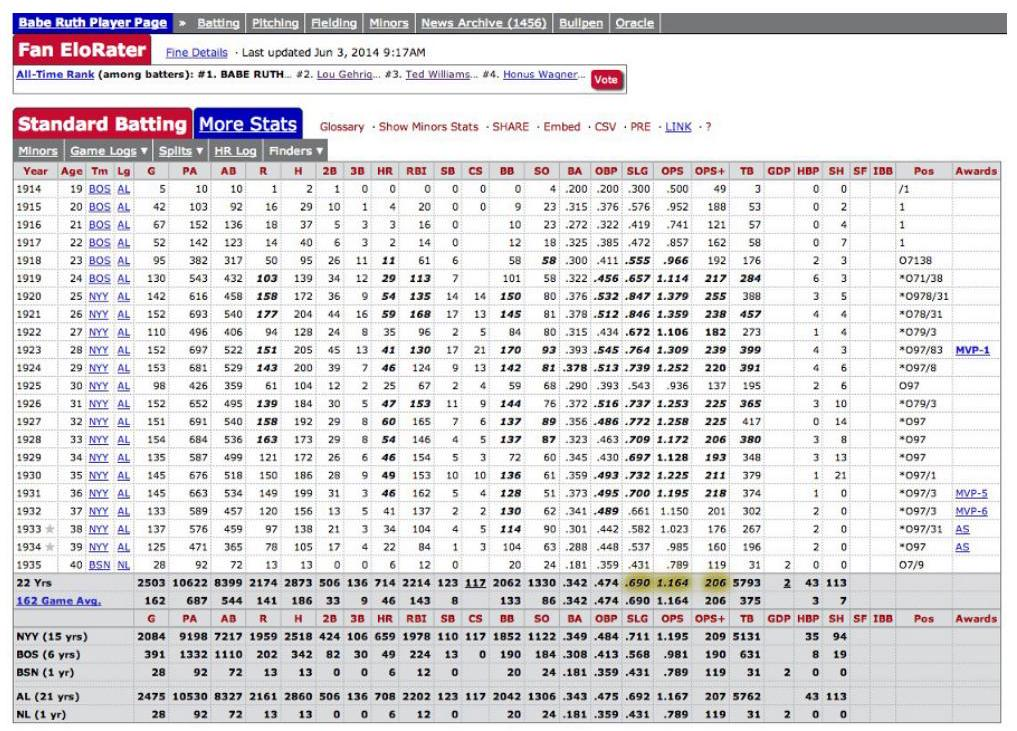
\includegraphics[max width=\textwidth]{2025_03_17_ca60ec0bfd96dcf8e028g-023}
    \caption{Statistical information on the performance of Babe Ruth can be found at \href{http://www.baseball-reference.com}{http://www.baseball-reference.com}.}
    \label{fig:babe_ruth}
\end{figure}

कुंजी व्यापक सोच रखना है: बड़े, सामान्य प्रश्नों के उत्तर अक्सर अत्यधिक-विशिष्ट डेटा सेट्स में छिपे होते हैं, जो इन्हें समाहित करने के लिए किसी भी तरह से डिज़ाइन नहीं किए गए थे।

\subsection{बेइसबॉल इनसाइक्लोपीडिया}
\index{baseball encyclopedia}बेइसबॉल लंबे समय से डेटा साइंस की दुनिया में एक महत्वपूर्ण स्थान रखता है। इस खेल को संयुक्त राज्य अमेरिका का राष्ट्रीय खेल कहा जाता है; वास्तव में, फ्रांसीसी इतिहासकार जेक्स बरज़ुन ने देखा कि "जो कोई भी अमेरिका के दिल और दिमाग को जानना चाहता है, उसे बेहतर होगा कि वह बेइसबॉल सीख ले।" मैं समझता हूँ कि कई पाठक अमेरिकी नहीं हैं, और जो हैं भी, वे खेल में पूरी तरह से रुचि नहीं रखते हो सकते हैं। लेकिन थोड़ी देर के लिए मेरे साथ बने रहें।\index{data!quantitative vs. categorical}\index{data!big vs. little}

क्या बनाता है बेसबॉल को डेटा विज्ञान के लिए महत्वपूर्ण, यह है इसके खेल का व्यापक सांख्यिकीय रिकॉर्ड, जो सौ साल से भी अधिक समय से है। बेसबॉल एक स्पोर्ट है विशिष्ट घटनाओं का: पिचर्स गेंद फेंकते हैं और बैटर उन्हें हिट करने की कोशिश करते हैं - जो स्वाभाविक रूप से सूचनात्मक सांख्यिकी को प्रोत्साहित करता है। प्रशंसक इन सांख्यिकियों में बच्चों के रूप में तल्लीन हो जाते हैं, विश्लेषण की मात्रात्मक शक्तियों और सीमाओं के बारे में अपनी संवेदनशीलता का निर्माण करते हैं। इनमें से कुछ बच्चे बड़े होकर डेटा वैज्ञानिक बनते हैं। वास्तव में, मूवी \textit{मनीबॉल} में ब्रैड पिट की सांख्यिकीय दृष्टिकोण वाली बेसबॉल टीम की सफलता अमेरिका के लोगों के लिए डेटा विज्ञान के साथ सबसे ज्वलंत संपर्क के रूप में बनी रहती है।

यह ऐतिहासिक बेसबॉल रिकॉर्ड \href{http://www.baseball-reference.com}{http://www.baseball-reference.com} पर उपलब्ध है। वहां, आपको हर खिलाड़ी के प्रदर्शन का संपूर्ण सांख्यिकीय डेटा मिलेगा, जिन्होंने कभी मैदान पर कदम रखा। इसमें प्रत्येक सीज़न के बल्लेबाज़ी, पिचिंग, और फील्डिंग रिकॉर्ड की संक्षिप्त सांख्यिकी शामिल है, साथ ही टीमों के बारे में जानकारी भी शामिल है।

%---- Page End Break Here ---- Page : 5

%--- Page 5 ---

\begin{figure}[h]
    \centering
    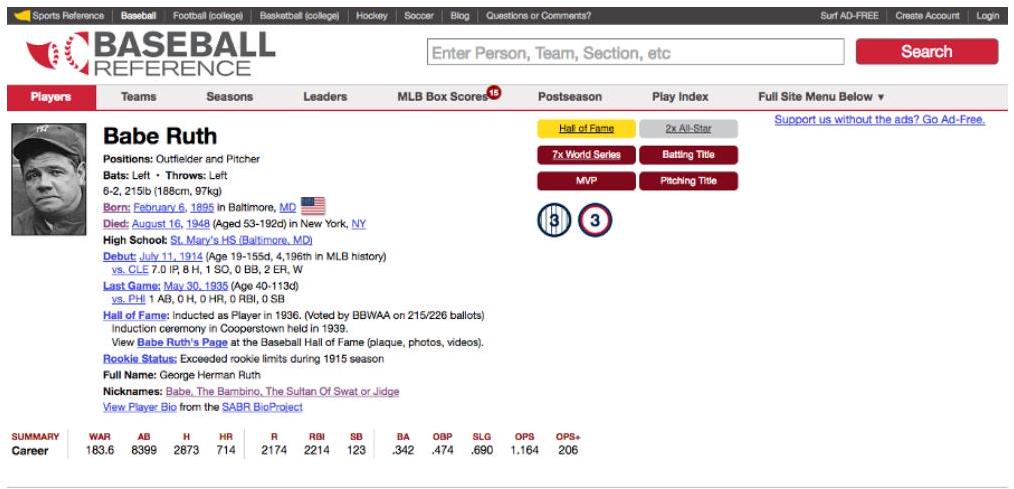
\includegraphics[max width=\textwidth]{2025_03_17_ca60ec0bfd96dcf8e028g-024}
    \caption{Personal information on every major league baseball player is available at \href{http://www.baseball-reference.com}{http://www.baseball-reference.com}.}
\end{figure}

लेकिन केवल सांख्यिकी से अधिक, सभी लोगों के जीवन और करियर का मेटाडेटा \index{metadata} है जिन्होंने कभी भी मेजर लीग बेसबॉल खेला है, जैसा कि चित्र 1.2 में दिखाया गया है। हमें प्रत्येक खिलाड़ी के महत्वपूर्ण सांख्यिकी (लंबाई, वजन, हाथियत) और उनके जीवनकाल (कब/कहाँ वे पैदा हुए और मरे) की जानकारी मिलती है। हमें वेतन जानकारी भी मिलती है (हर सीजन में प्रत्येक खिलाड़ी को कितना भुगतान किया गया) और लेन-देन डेटा (वे कैसे उस टीम की संपत्ति बने जिसके लिए उन्होंने खेला) भी मिलता है।

अब, मुझे एहसास हुआ कि आप में से कई लोगों को बेज़बॉल का बिल्कुल भी ज्ञान या रुचि नहीं है। यह खेल कुछ हद तक क्रिकेट की याद दिलाता है, अगर इससे मदद मिलती है। लेकिन याद रखें कि एक डेटा वैज्ञानिक के रूप में, आपके लिए अपने आसपास की दुनिया में रुचि लेना आपका काम है। इसे कुछ सीखने का एक अवसर समझें।

तो आप इस बेसबॉल डेटा सेट के साथ कौन से रोचक सवालों का जवाब दे सकते हैं? आगे बढ़ने से पहले पाँच सवाल लिखने की कोशिश करें। चिंता न करें, मैं आपके ख़त्म करने का इंतज़ार यहाँ करूँगा।

इस डेटा के साथ जिन प्रश्नों का उत्तर देना सबसे स्पष्ट होता है, वे सीधे तौर पर बेसबॉल से संबंधित होते हैं:

\begin{itemize}
  \item हम किसी व्यक्तिगत खिलाड़ी के कौशल या मूल्य को कैसे सबसे अच्छे तरीके से माप सकते हैं?\index{classification}\index{data science television}\index{Quant Shop}
  \item टीमों के बीच ट्रेड आमतौर पर कितनी निष्पक्षता से काम करते हैं?
  \item जब खिलाड़ी परिपक्व होते हैं और बड़े होते जाते हैं, तो उनके प्रदर्शन स्तर की सामान्य दिशा क्या होती है?
  \item बल्लेबाजी प्रदर्शन किस हद तक खेली जाने वाली स्थिति के साथ संबंधित होती है? उदाहरण के लिए, क्या आउटफील्डर्स वास्तव में इनफील्डर्स से बेहतर हिटर होते हैं?
\end{itemize}

ये रोचक प्रश्न हैं। लेकिन इससे भी अधिक रोचक हैं जनसांख्यिकीय और सामाजिक मुद्दों के बारे में प्रश्न। लगभग 20,000 प्रमुख लीग बेसबॉल खेल-

%--- Page 6 ---

पिछले 150 वर्षों में खिलाड़ियों ने मैदान सँभाला है, जिससे एक बड़ा, व्यापक रूप से प्रलेखित पुरुषों का समूह तैयार हुआ है जो बड़े, कम प्रलेखित जनसंख्या के लिए एक प्राथमिक नमूने के रूप में काम कर सकते हैं। वास्तव में, हम इस बेसबॉल खिलाड़ी डेटा का उपयोग इस प्रकार के प्रश्नों के उत्तर देने के लिए कर सकते हैं:

\begin{itemize}
  \item क्या बाएं हाथ वाले लोगों की जीवन अवधि दाएं हाथ वालों से कम होती है? हेंडेडनेस ज्यादातर जनसांख्यिकीय डेटा सेट्स में दर्ज नहीं किया गया है, लेकिन इसे यहाँ सावधानीपूर्वक एकत्र किया गया है। वास्तव में, इस डेटा सेट के विश्लेषण का उपयोग यह दिखाने के लिए किया गया है कि दाएं हाथ वाले लोग बायां हाथ वालों से लंबा जीते हैं [\cite{halpern1988right}]।
  \item लोग कितनी बार उसी स्थान पर वापस रहते हैं जहाँ वे पैदा हुए थे? जन्म और मृत्यु के स्थान को इस डेटा सेट में व्यापक रूप से रिकॉर्ड किया गया है। इसके अतिरिक्त, लगभग सभी लोगों ने अपने करियर का कम से कम एक हिस्सा घर से दूर खेला, जिसने उन्हें युवा अवस्था के महत्वपूर्ण समय में व्यापक दुनिया के संपर्क में लाया।
  \item क्या खिलाड़ी के वेतन सामान्यतः भूतकाल, वर्तमान, या भविष्य की प्रदर्शन की झलक देते हैं?
  \item कितने हद तक उँचाइयाँ और वजन व्यापक आबादी में बढ़ रहे हैं?
\end{itemize}

यहाँ दो विशेष विषयों के प्रति सजग रहने की आवश्यकता है। पहला, पहचानकर्ता और संदर्भ टैग (अर्थात् मेटाडेटा) अक्सर डेटा सेट में उस चीज़ से अधिक रोचक साबित होते हैं जिसकी हमें परवाह करनी चाहिए, यहाँ खेल का सांख्यिकीय रिकॉर्ड।

दूसरा है एक \textit{सांख्यिकीय प्रॉक्सी} का विचार,\index{statistical proxy} जहाँ आप अपने पास मौजूद डेटा सेट का उपयोग उस सेट के लिए स्थानापन्न करने के लिए करते हैं जिसे आप वास्तव में चाहते हैं। आपके सपनों का डेटा सेट शायद अस्तित्व में न हो, या यदि हो भी तो, शायद किसी कंपनी की दीवार के पीछे बंद हो सकता है। एक अच्छा डेटा वैज्ञानिक एक व्यवहारवादी होता है, जो यह देखता है कि जो उनके पास है उसके साथ वे क्या कर सकते हैं, बजाय इस बात की शिकायत करने के कि वे क्या हासिल नहीं कर सकते।

\subsection{इंटरनेट मूवी डेटाबेस (आईएमडीबी)}
\index{Internet Movie Database}\index{IMDb}
हर कोई फिल्मों से प्यार करता है। इंटरनेट मूवी डेटाबेस (आईएमडीबी) फिल्म उद्योग के सभी पहलुओं के बारे में भीड़ से मिली और संकलित की गई जानकारी उपलब्ध कराता है, at \href{http://www.imdb.com}{www.imdb.com}। आईएमडीबी वर्तमान में 3.3 मिलियन से अधिक फिल्में और टीवी कार्यक्रमों पर डेटा शामिल करता है। प्रत्येक फिल्म के लिए, आईएमडीबी में उसका शीर्षक, चलने का समय, शैलियाँ, रिलीज़ की तारीख, और कलाकारों और क्रू की पूरी सूची शामिल होती है। प्रत्येक प्रोडक्शन के बारे में वित्तीय जानकारी भी होती है, जिसमें फिल्म बनाने का बजट और बॉक्स ऑफिस पर उसकी सफलता शामिल होती है।

अंत में, प्रत्येक फिल्म के लिए दर्शकों और आलोचकों द्वारा व्यापक रेटिंग्स होती हैं। यह रेटिंग डेटा शून्य से दस सितारों के पैमाने पर प्राप्त अंकों से बना होता है, जो आयु और लिंग के आधार पर औसत में वर्गीकृत होता है। अक्सर लिखित समीक्षाएँ शामिल होती हैं, जिसमें समझाया जाता है कि किसी विशेष आलोचक ने क्यों एक निश्चित संख्या में सितारे दिए। फ़िल्मों के बीच भी लिंक होते हैं: उदाहरण के लिए, पहचान करना कि किन अन्य फ़िल्मों को \textit{इट्स अ वंडरफुल लाइफ} के दर्शकों द्वारा सबसे अधिक देखा गया है।

प्रत्येक अभिनेता, निर्देशक, निर्माता, और फिल्म से जुड़े कर्मीदल के सदस्य के पास IMDb में एक प्रविष्टि होनी चाहिए, जिसमें अब 6.5 मिलियन लोगों का रिकॉर्ड शामिल है।

%---- Page End Break Here ---- Page : 7

\clearpage
\label{अनुभाग:प्रश्न_डेटा}

\begin{figure}
  \centering
  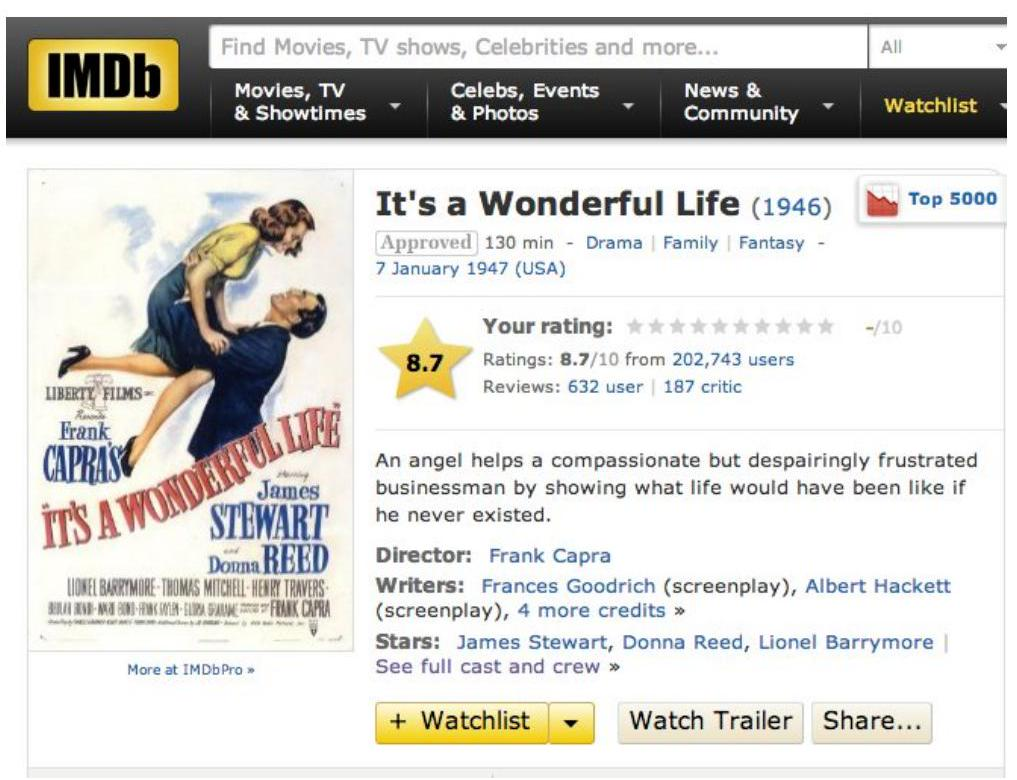
\includegraphics[max width=\textwidth]{2025_03_17_ca60ec0bfd96dcf8e028g-026}\index{General Sentiment}\index{natural language processing}\index{Stony Brook University}\index{Wikipedia}\index{genius}\index{wisdom}
  \caption{Representative film data from the Internet Movie Database.}
  \label{fig:imdb_film_data}
\end{figure}

\begin{figure}
  \centering
  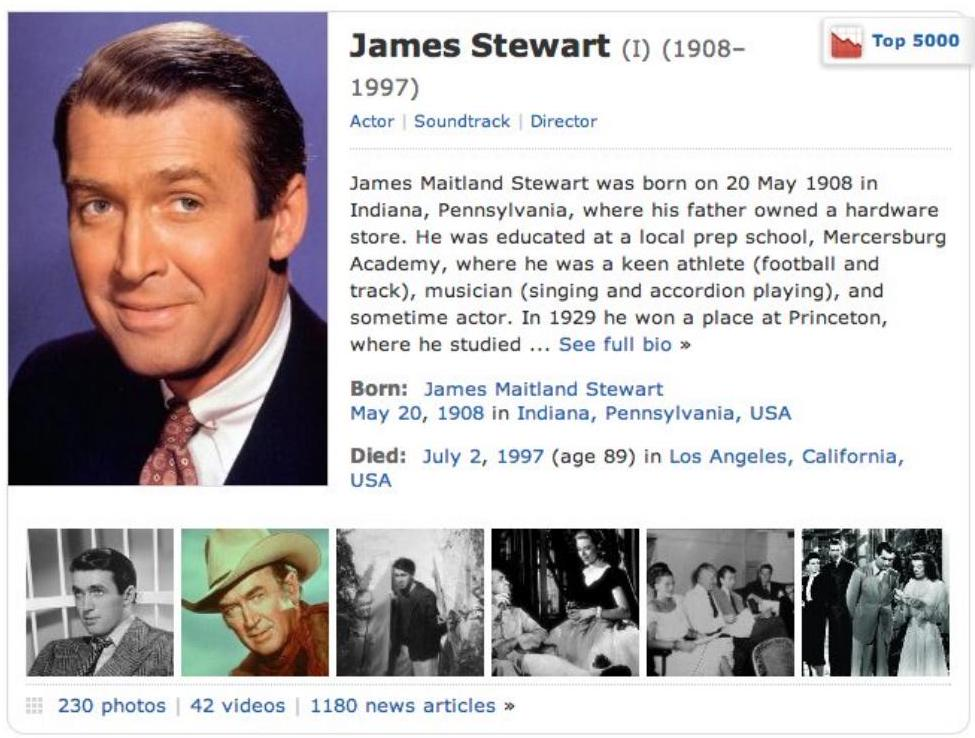
\includegraphics[max width=\textwidth]{2025_03_17_ca60ec0bfd96dcf8e028g-026(1)}
  \caption{Representative actor data from the Internet Movie Database.}
  \label{fig:imdb_actor_data}
\end{figure}

इनमें मेरे भाई, चचेरे भाई, और भाभी शामिल हैं। प्रत्येक अभिनेता हर फिल्म से जुड़ा हुआ है जिसमें उन्होंने भाग लिया, उनके किरदार के विवरण और क्रेडिट्स में उनकी स्थान के साथ। प्रत्येक व्यक्ति से संबंधित उपलब्ध डेटा में जन्म/मृत्यु तिथियां, ऊंचाई, पुरस्कार, और पारिवारिक संबंध शामिल हैं।

तो आप इस फिल्म डेटा के साथ किस प्रकार के प्रश्नों का उत्तर दे सकते हैं?

शायद IMDb से पूछे जाने वाले सबसे स्वाभाविक प्रश्नों में फिल्मों और अभिनेताओं के अत्यधिक पहलुओं की पहचान करना शामिल है:

\begin{itemize}
  \item कौन से अभिनेता सबसे अधिक फिल्मों में दिखाई दिए? सबसे अधिक पैसा कमाया? सबसे कम रेट की गई फिल्मों में दिखाई दिए? सबसे लंबा करियर या सबसे छोटा जीवनकाल किसका था?
  \item प्रत्येक वर्ष में सबसे उच्च रेटिंग वाली फिल्म कौन सी थी, या प्रत्येक विधा में सबसे अच्छी किसके पास थी? कौन सी फिल्मों ने सबसे अधिक पैसा खोया, सबसे शक्तिशाली कलाकारों के साथ थीं, या सबसे कम अनुकूल समीक्षाएँ मिलीं?
\end{itemize}

फिर वहाँ बड़े पैमाने पर प्रश्न होते हैं जिन्हें कोई चलचित्र व्यवसाय की प्रकृति के बारे में पूछ सकता है:

\begin{itemize}
  \item क्या फिल्म की आय दर्शकों की रेटिंग्स या पुरस्कारों के साथ कितना अनुरूप होती है? क्या ग्राहक स्वभाविक रूप से खराब फिल्मों की ओर जाते हैं, या रचनात्मक टीम के गुणों को सही से पुरस्कृत किया जाता है?
  \item रेटिंग्स, बजट और आय के संदर्भ में हॉलीवुड फिल्मों की तुलना बॉलीवुड फिल्मों से कैसे की जाती है? क्या अमेरिकी फिल्में विदेशी फिल्मों की तुलना में बेहतर स्वागत करती हैं, और यह अंतर्राष्ट्रीय और घरेलू समीक्षकों के बीच कैसे भिन्न होता है?
  \item फिल्मों में कलाकारों की आयु वितरण क्या है? औसतन, पत्नी का किरदार निभाने वाली अभिनेत्री पति का किरदार निभाने वाले अभिनेता से कितनी छोटी होती है? क्या समय के साथ यह असमानता बढ़ रही है या घट रही है?
  \item तेज़ जीयो, युवा मरो, और एक अच्छा दिखने वाला शव छोड़ो? क्या फिल्म सितारे सामान्य जनसंख्या की तुलना में छोटे या लंबे जीवन जीते हैं? या छोटे भूमिकाओं वाले कलाकारों की तुलना में?
\end{itemize}

मान लेते हैं कि एक फिल्म पर काम कर रहे लोग एक-दूसरे को जान लेते हैं, तो कास्ट और क्रू डेटा का उपयोग फिल्म व्यवसाय का एक सामाजिक नेटवर्क बनाने के लिए किया जा सकता है। अभिनेताओं का सामाजिक नेटवर्क कैसा दिखता है? द ओरैकल ऑफ बेकन\\index{Oracle of Bacon}फुटनोट{\url{https://oracleofbacon.org/}} केविन बेकन को हॉलीवुड ब्रह्मांड के केंद्र के रूप में दर्शाता है और किसी अन्य अभिनेता से बेकन तक का सबसे छोटा रास्ता उत्पन्न करता है। अन्य अभिनेता, जैसे सैमुएल एल. जैक्सन, भी और अधिक केंद्रीय सिद्ध होते हैं।

और अधिक महत्वपूर्ण रूप से, क्या हम इस डेटा का विश्लेषण करके यह निर्धारित कर सकते हैं कि किसी को एक विशेष फिल्म पसंद आएगी या नहीं? \textit{सहयोगी फ़िल्टरिंग} की तकनीक उन लोगों को खोजती है जिन्हें वे फ़िल्में पसंद आईं जो मुझे भी पसंद थीं, और उन फ़िल्मों की सिफारिश करती है जो उन्हें अच्छी लगीं, मेरे लिए अच्छे उम्मीदवार के रूप में। 2007 का Netflix पुरस्कार \$1,000,000 की प्रतिस्पर्धा थी ताकि एक रेटिंग इंजन उत्पादित किया जा सके जो निजी Netflix प्रणाली से 10\% बेहतर हो। इस पुरस्कार के अंतिम विजेता (BellKor) ने विभिन्न डेटा स्रोतों और तकनीकों का उपयोग किया, जिसमें लिंक्स का विश्लेषण भी शामिल था~\cite{bell2007lessons}.\index{sabermetrics}

\clearpage
\subsection{गूगल एनग्राम्स}\label{उप अनुभाग: गूगल एनग्राम्स}

\begin{figure}
  \centering
  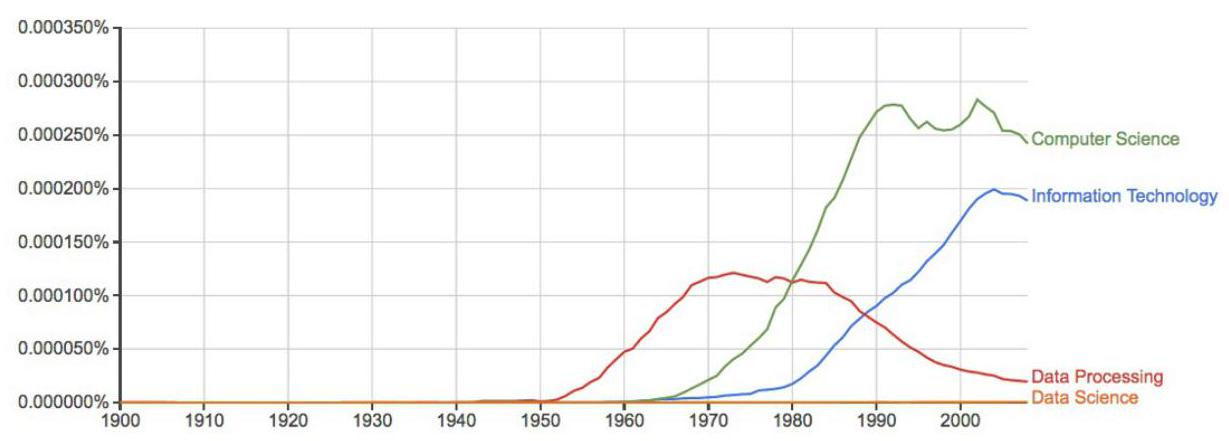
\includegraphics[max width=\textwidth]{2025_03_17_ca60ec0bfd96dcf8e028g-028}
  \caption{The rise and fall of data processing, as witnessed by Google Ngrams.}
  \label{fig:google_ngrams}
\end{figure}

मुद्रित पुस्तकें गुटेनबर्ग के 1439 में चल-प्रकार के आविष्कार के बाद से मानव ज्ञान का मुख्य भंडार रही हैं। भौतिक वस्तुएँ आज की डिजिटल दुनिया में कुछ असुविधा से जीती हैं, लेकिन प्रौद्योगिकी के पास हर चीज़ को डेटा में परिवर्तित करने का उपाय होता है। दुनिया की जानकारी व्यवस्थित करने के अपने मिशन के तहत, गूगल ने विश्व की सभी प्रकाशित पुस्तकों को स्कैन करने का प्रयास किया। वे अभी तक पूरी तरह से वहां नहीं पहुँचे हैं, लेकिन अब तक डिजिटलीकृत की गई 30 मिलियन पुस्तकें अब तक प्रकाशित सभी पुस्तकों का 20% से अधिक हिस्सा प्रस्तुत करती हैं।

गूगल इस डेटा का उपयोग खोज परिणामों में सुधार करने और प्रिंट से बाहर हो चुकी पुस्तकों तक नई पहुँच प्रदान करने के लिए करता है। लेकिन शायद सबसे अद्भुत उत्पाद है\textit{गूगल एनग्राम्स}, जो सांस्कृतिक समय की धारा में बदलावों की निगरानी के लिए एक अद्वितीय संसाधन है। यह हमें यह जानने की सुविधा देता है कि प्रत्येक वर्ष प्रकाशित पुस्तकों में कितनी बार छोटी वाक्यांशों का प्रचलन होता है। प्रत्येक वाक्यांश को उनके स्कैन की गई पुस्तक संग्रह में कम से कम चालीस बार आना चाहिए। इससे अस्पष्ट शब्द और वाक्यांश को हटा दिया जाता है, लेकिन फिर भी विश्लेषण के लिए दो अरब से अधिक समय श्रृंखलाएँ उपलब्ध रहती हैं।

यह समृद्ध डेटा सेट दर्शाता है कि पिछले 200 वर्षों में भाषा उपयोग में कैसे परिवर्तन हुआ है, और इसे व्यापक रूप से सांस्कृतिक प्रवृत्ति विश्लेषण में लागू किया गया है~\cite{MAV+11}। चित्र~\ref{fig:google_ngrams}में यह डेटा दिखाया गया है कि किस प्रकार शब्द\textit{data}कंप्यूटिंग के संदर्भ में उपयोग से बाहर हो गया।\textit{Data processing}1950 के पंच कार्ड और घूमने वाले चुम्बकीय टेप के युग में कंप्यूटिंग क्षेत्र से जुड़ा एक लोकप्रिय शब्द था। एनग्राम्स डेटा दिखाता है कि\textit{Computer Science}के तीव्र उदय ने 1980 तक\textit{Data Processing}को पीछे नहीं छोड़ा। यहां तक कि आज भी,\textit{Data Science}इस पैमाने पर लगभग अदृश्य बना हुआ है।

Google Ngrams को\url{http://books.google.com/ngrams} पर देखें। मैं वादा करता हूँ कि आपको इसके साथ खेलकर मजा आएगा। \textit{hot dog}को \textit{tofu}से, \textit{science}को \textit{religion}से, \textit{freedom}को \textit{justice}से, और \textit{sex}को \textit{marriage}से तुलना करें, और इस अद्भुत दूरबीन के माध्यम से अतीत में झांकने के बारे में बेहतर समझ प्राप्त करें।

लेकिन जब आप खेलना पूरा कर लें, तो उन बड़े कामों के बारे में सोचें जो आप इस डेटा के साथ कर सकते हैं। मान लें कि आपके पास पिछले 200 वर्षों में प्रकाशित पुस्तकों में \textit{सभी} शब्दों/वाक्यांशों के वार्षिक संदर्भों की संख्या तक पहुंच है।

%---- Page End Break Here ---- Page : 10



गूगल इस डेटा को मुक्त रूप से उपलब्ध कराता है। तो आप इसके साथ क्या करने जा रहे हैं?

विशिष्ट शब्दों से संबंधित समय श्रृंखलाओं को Ngrams Viewer का उपयोग करके देखना मजेदार है। लेकिन कई समय श्रृंखलाओं को एकत्रित करके अधिक जटिल ऐतिहासिक रुझानों को पकड़ा जा सकता है। निम्नलिखित प्रकार के प्रश्न मुझे विशेष रूप से दिलचस्प लगते हैं:

\begin{itemize}
  \item समय के साथ गाली-गलौज की मात्रा में कैसे परिवर्तन आया है? मेरे सबसे परिचित चार-अक्षरीय शब्दों का उपयोग 1960 के बाद से बहुत बढ़ गया है, हालांकि यह स्पष्ट नहीं है कि यह बढ़ते गाली-गलौज को दर्शाता है या प्रकाशन के मानकों में कमी को।
  \item नए शब्द कितनी बार उभरते हैं और लोकप्रिय होते हैं? क्या ये शब्द आम उपयोग में बने रहते हैं, या जल्दी से लुप्त हो जाते हैं? क्या हम यह पता लगा सकते हैं कि समय के साथ शब्दों का अर्थ कैसे बदलता है, जैसे \textit{gay} का \textit{happy} से \textit{homosexual} में बदलाव?
  \item क्या समय के साथ वर्तनी के मानक सुधर रहे हैं या बिगड़ रहे हैं, विशेषकर अब जब हम स्वचालित स्पेल चेकिंग के युग में प्रवेश कर चुके हैं? शायद ही कभी उपयोग किए जाने वाले शब्द जो सामान्यतः उपयोग किए गए शब्द से केवल एक अक्षर हटे हुए होते हैं, वर्तनी त्रुटियों के संभावित उम्मीदवार होते हैं (जैसे \textit{algorithm} बनाम \textit{algorthm})। कई विभिन्न गलतियों के संकलन पर, क्या ऐसी त्रुटियाँ बढ़ रही हैं या घट रही हैं?
\end{itemize}

आप इस एनग्राम्स कॉर्पस का उपयोग करके एक भाषा मॉडल बना सकते हैं जो किसी दिए गए भाषा में शब्दों के अर्थ और उपयोग को पकड़ता है। हम सेक्शन 11.6.3 में वर्ड एम्बेडिंग्स पर चर्चा करेंगे, जो भाषा मॉडल बनाने के लिए शक्तिशाली उपकरण हैं। आवृत्ति गणना यह प्रकट करती है कि कौन से शब्द सबसे लोकप्रिय हैं। एक-दूसरे के बगल में आने वाले शब्द जोड़े की आवृत्ति को भाषण पहचान प्रणाली में सुधार के लिए उपयोग किया जा सकता है, यह पहचानने में मदद करते हुए कि वक्ता ने \textit{that's too bad} या \textit{that's to bad} कहा। ये लाखों किताबें प्रतिनिधि मॉडल बनाने के लिए एक पर्याप्त डेटासेट प्रदान करती हैं।

\subsection{न्यू यॉर्क टैक्सी रिकॉर्ड}

हर वित्तीय लेन-देन आजकल अपने पीछे डेटा ट्रेल छोड़ता है। इन पथों का पालन करके रोचक अंतर्दृष्टियों तक पहुँचा जा सकता है।

टैक्सी कैब शहर के परिवहन नेटवर्क का एक महत्वपूर्ण हिस्सा बनाते हैं। वे शहर की सड़कों पर ग्राहक ढूँढने के लिए घूमती रहती हैं, और फिर उन्हें उनकी यात्रा की लंबाई के अनुसार किराया लेकर उनकी मंज़िल तक पहुँचाती हैं। प्रत्येक कैब में एक मीटरिंग डिवाइस होता है जो यात्रा की लागत को समय के अनुसार गणना करता है। यह मीटर रिकॉर्ड रखने के उपकरण के रूप में कार्य करता है, और यह सुनिश्चित करने के लिए एक तंत्र होता है कि चालक प्रत्येक यात्रा के लिए उचित शुल्क ले।

न्यूयॉर्क टैक्सियों में वर्तमान में उपयोग किए जा रहे टैक्सी मीटर किराए की गणना के अलावा और भी कई चीजें कर सकते हैं। ये क्रेडिट कार्ड टर्मिनल के रूप में कार्य करते हैं, प्रदान करते हुए एक तरीका

\begin{figure}[h]
\centering
\begin{tabular}{|c|c|c|c|c|c|c|c|c|c|}
\hline
Vendor ID & passenger count & trip distance & pickup longitude & \begin{tabular}{l}
pickup\_ \\
latitude \\
\end{tabular} & dropoff longitude & dropoff\_ & payment type & \( \begin{aligned} & \text { tip_- } \\ & \text { amount } \end{aligned} \) & total amount \\
\hline
2 & 1 & 7.22 & -73.9998 & 40.74334 & -73.9428 & 40.80662 & 2 & 0 & 30.8 \\
\hline
1 & 1 & 2.3 & -73.977 & 40.7749 & -73.9783 & 40.74986 & 1 & 2.93 & 16.23 \\
\hline
1 & 1 & 1.5 & -73.9591 & 40.77513 & -73.9804 & 40.78231 & 1 & 1.65 & 9.95 \\
\hline
1 & 1 & 0.9 & -73.9766 & 40.78075 & -73.9706 & 40.78885 & 1 & 1.45 & 8.75 \\
\hline
2 & 1 & 2.44 & -73.9786 & 40.78592 & -73.9974 & 40.7563 & 1 & 2 & 16.3 \\
\hline
2 & 1 & 3.36 & -73.9764 & 40.78589 & -73.9424 & 40.82209 & 1 & 3.58 & 17.88 \\
\hline
2 & 2 & 2.34 & -73.9862 & 40.76087 & -73.9569 & 40.77156 & 1 & 1 & 13.8 \\
\hline
2 & 1 & 10.19 & -73.79 & 40.64406 & -73.9312 & 40.67588 & 2 & 0 & 32.8 \\
\hline
1 & 2 & 3.3 & -73.9937 & 40.72738 & -73.9982 & 40.7641 & 1 & 2 & 21.3 \\
\hline
1 & 1 & 1.8 & -73.9949 & 40.74006 & -73.9767 & 40.74934 & 1 & 1.85 & 11.15 \\
\hline
\end{tabular}
\caption{Representative fields from the New York city taxi cab data: pick up and dropoff points, distances, and fares.}
\end{figure}

ग्राहकों के लिए राइड के लिए नगद के बिना भुगतान करना आसान हो सके। ये ग्लोबल पोज़िशनिंग सिस्टम्स\index{Global Positioning System} (जीपीएस) के साथ एकीकृत होते हैं, जो प्रत्येक पिकअप और ड्रॉप ऑफ की सटीक स्थान को रिकॉर्ड करते हैं। और अंत में, क्योंकि वे वायरलेस नेटवर्क पर हैं, ये बॉक्स सभी डेटा को एक केंद्रीय सर्वर को संप्रेषित कर सकते हैं।

परिणाम एक डाटाबेस है जो दुनिया के महानतम शहरों में से एक, हर एक टैक्सी कैब की प्रत्येक यात्रा का दस्तावेजीकरण करता है, जिसका एक छोटा सा हिस्सा चित्र 1.6 में दिखाया गया है। क्योंकि न्यूयॉर्क टैक्सी और लिमोजीन कमीशन एक सार्वजनिक एजेंसी है, इसकी गैर-गोपनीय डेटा सभी के लिए सूचना की स्वतंत्रता अधिनियम (एफओए) के तहत उपलब्ध है।

हर यात्रा दो अभिलेख उत्पन्न करती है: एक यात्रा के डेटा के साथ, दूसरा किराए के विवरण के साथ। प्रत्येक यात्रा को प्रत्येक गाड़ी के पदक (लाइसेंस) के साथ और प्रत्येक चालक के पहचानकर्ता के साथ जोड़ा जाता है। प्रत्येक यात्रा के लिए, हमें उठाने और छोड़ने का समय/तिथि मिलती है, साथ ही प्रारंभिक स्थान और गंतव्य के जीपीएस निर्देशांक (देशांतर और अक्षांश) मिलते हैं। हमें इन बिंदुओं के बीच वे कौन सा मार्ग यात्रा करते हैं, इसके जीपीएस डेटा नहीं मिलता है, लेकिन कुछ हद तक इसे उनके बीच के सबसे छोटे रास्ते से अनुमान लगाया जा सकता है।

भाड़े के डेटा के लिए, हम प्रत्येक यात्रा की मीटर की गई लागत प्राप्त करते हैं, जिसमें कर, अधिभार और टोल शामिल हैं। सेवा के लिए ड्राइवर को एक टिप देना पारंपरिक है, जिसकी राशि भी डेटा में दर्ज की जाती है।

तो मैं तुमसे बात कर रहा हूँ। यह टैक्सी डेटा आसानी से उपलब्ध है, जिसमें पिछले कई वर्षों में 80 मिलियन से अधिक यात्राओं के रिकॉर्ड शामिल हैं। आप इसके साथ क्या करने जा रहे हैं?

कोई भी रोचक डेटा सेट का उपयोग विभिन्न स्तरों पर प्रश्नों के उत्तर देने के लिए किया जा सकता है। यह टैक्सी किराया डेटा हमें परिवहन उद्योग को बेहतर तरीके से समझने में मदद कर सकता है, लेकिन यह भी कि शहर कैसे काम करता है और हम इसे और बेहतर कैसे बना सकते हैं। टैक्सी उद्योग के संदर्भ में प्राकृतिक प्रश्नों में शामिल हैं:

%---- Page End Break Here ---- Page : 12



\label{अनुभाग:प्रश्न_पूछना}

\begin{figure}[h]
    \centering
    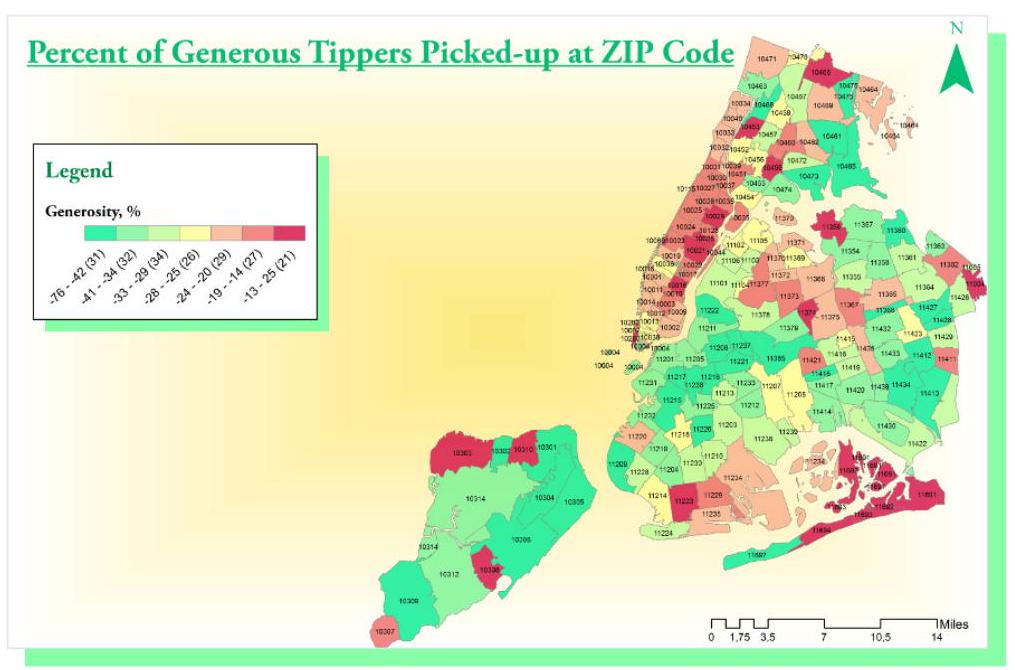
\includegraphics[max width=\textwidth]{2025_03_17_ca60ec0bfd96dcf8e028g-031}
    \caption{Which neighborhoods in New York City tip most generously? The relatively remote outer boroughs of Brooklyn and Queens, where trips are longest and supply is relatively scarce.}\index{conditional probability}\index{Fermat, Pierre de}\index{independence}\index{Pascal, Blaise}\index{conditional probability}
    \label{fig:nyc_neighborhoods}
\end{figure}

\begin{itemize}
  \item औसतन, चालक प्रत्येक रात कितने पैसे कमाते हैं? वितरण क्या है? क्या चालक धूप वाले दिनों में अधिक कमाते हैं या बरसात के दिनों में?
  \item शहर में कौन से स्थान चालक के लिए लाभदायक भाड़े उठाने के लिए सबसे अच्छे हैं? दिन के विभिन्न समयों पर यह कैसे बदलता है?
  \item चालक रात के काम के दौरान कितनी दूर यात्रा करते हैं? हम इस डेटा सेट का उपयोग करके इसे सटीक रूप से नहीं बता सकते, क्योंकि यह भाड़ों के बीच यात्रा किए गए रूट का जीपीएस डेटा नहीं प्रदान करता। लेकिन हमें अंतिम स्थान छोड़ने का स्थान, अगली बार उठाने का स्थान, और उनके बीच का समय पता है। ये जानकारी एक सही अनुमान लगाने के लिए पर्याप्त होनी चाहिए।
  \item कौन से चालक अपने अचकित बाहर से आए यात्रियों को "सफर" कराते हैं, किराया बढ़ाने के लिए, जो कि एक बहुत ही छोटा, सस्ता सफर होना चाहिए था?
  \item चालक कितनी टिप्स पाते हैं, और क्यों? क्या तेजी से चलने वाले चालकों को बेहतर टिप्स मिलती हैं? पड़ोस के हिसाब से टिपिंग दर कैसे बदलती है, और क्या यह अमीर या गरीब पड़ोस हैं जो अधिक उदार साबित होते हैं? मैं स्वीकार करूंगा कि हमने इसका विश्लेषण किया, जिसे मैं खंड~\ref{sec:war_story_taxi_deriver} के युद्ध कहानी में और अधिक वर्णन करूँगा। हमने विविध दिलचस्प पैटर्न पाए \cite{starov2015gis}. चित्र~\ref{fig:nyc_neighborhoods} दर्शाता है कि मैनहट्टनाइट्स आम तौर पर ब्रूकलिन, क्वींस, और स्टेटन आइलैंड के बड़े हिस्सों की तुलना में मितव्ययी होते हैं, जहां यात्राएं लंबी होती हैं और सड़क के टैक्सी एक दुर्लभ लेकिन स्वागत योग्य दृश्य होते हैं।
\end{itemize}

लेकिन असली सवाल शहर में परिवहन को समझने के बारे में हैं। हम टैक्सी यात्रा के समयों का उपयोग शहर में यातायात के स्तर को एक सूचक के रूप में मापने के लिए कर सकते हैं, और वह भी बहुत बारीकी से। भीड़भाड़ के समय यातायात अन्य समयों की तुलना में कितना धीमा होता है, और देरी सबसे ज्यादा कहाँ होती है? समस्या क्षेत्रों की पहचान करना समाधान प्रस्तावित करने की दिशा में पहला कदम है, जैसे कि यातायात बत्तियों के समय के पैटर्न को बदलना, अधिक बसें चलाना, या केवल उच्च-संख्या वाले यात्री गलियाँ बनाना।

उसी प्रकार, हम टैक्सी डेटा का उपयोग करके शहर के विभिन्न क्षेत्रों के बीच परिवहन प्रवाह को माप सकते हैं। लोग दिन के विभिन्न समयों पर कहाँ यात्रा कर रहे हैं? यह हमें केवल भीड़भाड़ से कहीं अधिक जानकारी देता है। टैक्सी डेटा को देखकर, हमें यह देखना चाहिए कि पर्यटक होटलों से आकर्षण स्थलों तक जा रहे हैं, अधिकारी शानदार मुहल्लों से वॉल स्ट्रीट तक और नशे में धुत लोग क्लबों से देर रात पार्टी के बाद घर लौट रहे हैं।

इस तरह का डेटा बेहतर परिवहन प्रणालियों को डिजाइन करने के लिए आवश्यक है। अगर एक अकेला यात्री बिंदु$a$से बिंदु$b$तक यात्रा कर रहा है, जबकि बिंदु$a+\epsilonपर एक और यात्री भी है जो वहां जाना चाहता है, तो यह अपव्ययी है। टैक्सी डेटा का विश्लेषण राइड-शेयरिंग प्रणाली का सटीक अनुकरण सक्षम करता है, ताकि हम इस तरह की सेवा की मांग और लागत में कमी का सटीक मूल्यांकन कर सकें।

\section{डाटा के गुणधर्म}
\index{data!properties}
यह पुस्तक डाटा के विश्लेषण की तकनीकों के बारे में है। लेकिन वह कौन सी मूलभूत चीज़ है जिसका हम अध्ययन करेंगे? यह खंड डाटा के गुणधर्मों की एक संक्षिप्त वर्गीकरण प्रदान करता है, ताकि हम बेहतर तरीके से समझ सकें और सराह सकें कि हम किन चीजों पर काम करेंगे।

\subsection{संगठित बनाम असंगठित डेटा}
\index{data!unstructured}\index{data!structured}
कुछ डेटा सेट अच्छी तरह से संगठित होते हैं, जैसे डेटाबेस या स्प्रेडशीट प्रोग्राम में तालिकाएं। अन्य दुनिया की स्थिति के बारे में जानकारी रिकॉर्ड करते हैं, लेकिन अधिक विविध तरीके से। शायद यह विकिपीडिया जैसी छवियों और लिंक के साथ एक बड़ा पाठ कॉर्पस है, या व्यक्तिगत चिकित्सा रिकॉर्ड में दिखाई देने वाले नोट्स और परीक्षण परिणामों का जटिल मिश्रण।

आम तौर पर, यह पुस्तक संरचित डेटा के साथ काम करने पर ध्यान केंद्रित करेगी। डेटा को अक्सर एक\textit{मैट्रिक्स} द्वारा प्रदर्शित किया जाता है,\index{matrix} जहां मैट्रिक्स की पंक्तियाँ अलग-अलग वस्तुओं या रिकॉर्ड्स का प्रतिनिधित्व करती हैं, और स्तंभ इन वस्तुओं की अलग-अलग विशेषताओं का प्रतिनिधित्व करते हैं। उदाहरण के लिए, अमेरिकी शहरों के बारे में डेटा सेट में प्रत्येक शहर के लिए एक पंक्ति हो सकती है, जिसमें राज्य, जनसंख्या और क्षेत्र जैसी विशेषताओं का प्रतिनिधित्व करने वाले स्तंभ होते हैं।

जब हमें एक असंरचित डेटा स्रोत, जैसे कि ट्विटर से ट्वीट्स का संकलन, का सामना करना पड़ता है, तो हमारा पहला कदम आमतौर पर इसे संरचना देने के लिए एक मैट्रिक्स बनाना होता है। एक \textit{शब्दों का थैला} मॉडल एक मैट्रिक्स का निर्माण करेगा जिसमें प्रत्येक ट्वीट के लिए एक पंक्ति होती है, और प्रत्येक अक्सर उपयोग किए जाने वाले शब्दावली शब्द के लिए एक स्तंभ होता है। मैट्रिक्स प्रविष्टि $M[i, j]$ तब दर्शाती है कि ट्वीट $i$ में कितनी बार शब्द $j$ मौजूद होता है। ऐसे मैट्रिक्स सूत्रीकरण हमारे \ref{रेखीय बीजगणित} पर चर्चा को अध्याय~⸨chap:linear_algebra⸩ में प्रेरित करेंगे।

%---- Page End Break Here ---- Page : 14
\subsection{Quantitative vs. Categorical Data}
\textit{Quantitative data} consists of numerical values, like height and weight. Such data can be incorporated directly into algebraic formulas and mathematical models, or displayed in conventional graphs and charts.

इसके विपरीत, \textit{श्रेणीबद्ध डेटा}उन लेबल्स से बना होता है जो जांच के तहत वस्तुओं की विशेषताओं का वर्णन करते हैं, जैसे लिंग, बालों का रंग, और पेशा। यह वर्णात्मक जानकारी संख्यात्मक डेटा के जितनी ही सटीक और अर्थपूर्ण हो सकती है, लेकिन इसे समान तकनीकों का उपयोग करके काम नहीं किया जा सकता।

श्रेणीबद्ध डेटा को आमतौर पर संख्यात्मक रूप से कोडित किया जा सकता है। उदाहरण के लिए, लिंग को\textit{मेल}$=0$या\textit{फीमेल}$=1$के रूप में प्रस्तुत किया जा सकता है। लेकिन चीजें अधिक जटिल हो जाती हैं जब प्रति विशेषता दो से अधिक पात्र होते हैं, विशेष रूप से जब उनके बीच कोई स्पष्ट क्रम नहीं होता है। हम हर शेड को एक विशिष्ट मान देकर बालों के रंगों को संख्याओं के रूप में कोड कर सकते हैं जैसे कि ग्रे हेयर$=0$, रेड हेयर$=1$, और ब्लॉन्ड हेयर$=2$। हालांकि, हम वास्तव में इन मूल्यों को संख्याओं के रूप में नहीं मान सकते, सरल पहचान परीक्षण के अलावा। अधिकतम या न्यूनतम बाल रंग के बारे में बात करना किस हद तक समझ में आता है? मेरे बालों के रंग से आपके बालों के रंग को घटाने का क्या अर्थ है?

हम इस पुस्तक में जो कुछ भी करेंगे, वह ज्यादातर संख्यात्मक डेटा के इर्द-गिर्द घूमेगा। लेकिन श्रेणीगत विशेषताओं और उनके लिए काम करने वाले तरीकों पर भी नज़र रखें। वर्गीकरण और क्लस्टरिंग विधियों को संख्यात्मक डेटा से श्रेणीगत लेबल उत्पन्न करने के रूप में देखा जा सकता है, और यह इस पुस्तक में एक प्रमुख ध्यान केंद्रित होगा।

\subsection{बिग डेटा बनाम लिटल डेटा}
डेटा विज्ञान \textit{बिग डेटा}, कंप्यूटर लॉग्स और सेंसर उपकरणों से प्राप्त विशाल डेटा सेट्स के विश्लेषण के साथ जनता की नजर में मिलकर रह गया है। सिद्धांत रूप में, अधिक डेटा होना हमेशा कम डेटा होने से बेहतर होता है, क्योंकि आप आवश्यकता पड़ने पर कुछ डेटा का नमूना करके उसे एक छोटे सेट में बदल सकते हैं।

बिग डेटा एक रोमांचक परिघटना है, और हम इसे अध्याय 12 में चर्चा करेंगे। लेकिन व्यवहार में, बड़े डेटा सेट के साथ काम करने में कठिनाइयाँ होती हैं। इस पुस्तक में, हम डेटा का विश्लेषण करने के लिए एल्गोरिदम और सर्वोत्तम अभ्यासों पर विचार करेंगे। सामान्यत: जब मात्रा बहुत अधिक हो जाती है तो चीजें कठिन हो जाती हैं। बिग डेटा की चुनौतियों में शामिल हैं:

\begin{itemize}\index{signal to noise ratio}\index{stock market}\index{variance!interpretation}
\item \textit{जैसे-जैसे डेटा का आकार बढ़ता है, विश्लेषण चक्र समय धीमा हो जाता है}: डेटा सेट्स पर कम्प्यूटेशनल ऑपरेशन्स की प्रक्रिया लंबे समय तक चलती है क्योंकि उनका आकार बढ़ता जाता है। छोटे स्प्रेडशीट्स त्वरित प्रतिक्रिया प्रदान करते हैं, जिससे आप प्रयोग और \textit{क्या होगा} जैसे सवालों से खेल सकते हैं? लेकिन बड़े स्प्रेडशीट्स के साथ काम करना धीमा और कठिन हो सकता है, और अत्यधिक विशाल डेटा सेट्स से उत्तर प्राप्त करने में कई घंटे या दिन लग सकते हैं।
\item \textit{बड़े डेटा सेट्स को विज़ुअलाइज़ करना जटिल होता है}: करोड़ों अंकों वाले प्लॉट्स को कंप्यूटर स्क्रीन या मुद्रित छवियों पर दिखाना असंभव होता है, इसे संकल्पात्मक रूप से समझने की तो बात ही छोड़िए। जब हम देख नहीं सकते हैं तो उसे वास्तव में समझने की हम उम्मीद कैसे कर सकते हैं? 
\item \textit{सरल मॉडल्स को फिट या मूल्यांकन करने के लिए विशाल डेटा की आवश्यकता नहीं होती}: एक सामान्य डेटा विज्ञान कार्य में कुछ चरों के आधार पर निर्णय लेना शामिल हो सकता है: जैसे कि, क्या मुझे इस व्यक्ति को जीवन बीमा देना चाहिए?) उम्र, लिंग, ऊँचाई, वजन, और मौजूदा चिकित्सा स्थितियों की उपस्थिति या अनुपस्थिति के आधार पर।
\end{itemize}

अगर मेरे पास 1 मिलियन लोगों पर यह डेटा उनके संबंधित जीवन परिणामों के साथ है, तो मैं कवरेज जोखिम के अच्छे सामान्य मॉडल का निर्माण कर पाने में सक्षम होना चाहिए। यदि मेरे पास यह डेटा सैकड़ों मिलियन लोगों पर होता तो शायद यह मुझे काफी बेहतर मॉडल बनाने में मदद नहीं करेगा। कुछ ही चर (जैसे आयु और वैवाहिक स्थिति) पर निर्णय मापदंड बहुत जटिल नहीं हो सकते, और यह बड़ी संख्या में आवेदकों पर मजबूती से लागू होना चाहिए। कोई भी अवलोकन जो इतना सूक्ष्म हो कि उसे बाहर निकालने के लिए विशाल डेटा की आवश्यकता हो, एक बड़े व्यवसाय के लिए अप्रासंगिक साबित होगा जो मात्रा पर आधारित है।

\textit{बिग डेटा}को कभी-कभी \textit{बैड डेटा}कहा जाता है। यह अक्सर एक दिए गए सिस्टम या प्रक्रिया के उप-उत्पाद के रूप में इकट्ठा किया जाता है, बजाय इसके कि आपके सामने प्रश्न का उत्तर देने के लिए इसे उद्देश्यपूर्ण तरीके से एकत्र किया गया हो। परिणामस्वरूप, हमें ऐसा कुछ समझने के लिए महान प्रयास करने पड़ सकते हैं, सिर्फ इसलिए कि हमारे पास यह है।

राष्ट्रपति उम्मीदवारों के बीच मतदाताओं की प्राथमिकताओं पर एक नज़र डालने की समस्या पर विचार करें। बड़े डेटा की दृष्टिकोण में संभवतः विशाल Twitter या Facebook फ़ीड्स का विश्लेषण किया जा सकता है, ताकि उनके विचारों के संकेतों को पाठ में समझा जा सके। छोटे डेटा की दृष्टिकोण में कदाचित एक सर्वेक्षण करना शामिल हो, जिसमें कुछ सौ लोगों से यह विशेष सवाल पूछकर परिणामों को संयोजित किया जाए। आप कौनसी प्रक्रिया को अधिक सटीक मानते हैं? सही डेटा सेट वह है जो हाथ के कार्यों के लिए सबसे सीधे प्रासंगिक हो, न कि आवश्यक रूप से सबसे बड़ा हो।

\textit{घर-पर पाठ}: बड़े आंकड़ों का अंधाधुंध विश्लेषण करने की आकांक्षा मत रखो। दिए गए प्रश्न का उत्तर देने के लिए \textit{सही} आंकड़ों की खोज करो, जरूरी नहीं है कि सबसे बड़े चीज की तलाश करो जो तुम्हारे हाथ लग सके।

\section{वर्गीकरण और प्रतिगमन}
\index{regression}पारंपरिक डेटा विज्ञान और पैटर्न पहचान अनुप्रयोगों में दो प्रकार की समस्याएँ बार-बार उत्पन्न होती हैं, वर्गीकरण और प्रतिगमन की चुनौतियाँ। जैसे-जैसे इस पुस्तक का विकास हुआ है, मैंने इन समस्याओं को हल करने के लिए एल्गोरिदमिक दृष्टिकोणों की चर्चाओं को बाद के अध्यायों की ओर धकेला है, ताकि वे डेटा संशोधन, सांख्यिकी, दृश्यता, और गणितीय मॉडलिंग में मूल सामग्री की दृढ़ समझ से लाभान्वित हो सकें।\index{characterizing distributions}\index{performance of models}

फिर भी, मैं वर्गीकरण और प्रतिगमन से संबंधित मुद्दों का उल्लेख करूंगा जब वे उत्पन्न होते हैं, इसलिए यह यहाँ एक त्वरित परिचय देने के लिए ठहरने का औचित्य रखता है, ताकि जब आप इन्हें देखे तो इन्हें पहचानने में मदद मिल सके।



% Continue with the rest of the content here.
%---- Page End Break Here ---- Page : 16



खेल प्रतियोगिता के परिणाम की भविष्यवाणी करना (टीम$A$या टीम$B$?) या दिए गए फिल्म की शैली का निर्णय लेना (कॉमेडी, ड्रामा, या एनिमेशन?) \textit{वर्गीकरण} समस्याएँ हैं, क्योंकि इनमें से प्रत्येक में संभावित विकल्पों से एक लेबल का चयन करना शामिल है।

\begin{itemize}
  \item \textit{पूर्वानुमान}: एक अन्य आम कार्य किसी दिए गए संख्यात्मक मात्रा का पूर्वानुमान लगाना है। किसी व्यक्ति का वजन या इस वर्ष हमें कितनी बर्फ मिलेगी, यह एक \textit{पूर्वानुमान} समस्या है, जहाँ हम पहले के मानों और अन्य प्रासंगिक विशेषताओं के संदर्भ में संख्यात्मक फ़ंक्शन के भविष्य के मान की भविष्यवाणी करते हैं।
\end{itemize}

शायद इरादतन विभाजन को समझने का सबसे अच्छा तरीका यह है कि विभिन्न डेटा विज्ञान समस्याओं को देखा जाए और उन्हें प्रतिगमन या वर्गीकरण के रूप में लेबल (वर्गीकृत) किया जाए। इन दो प्रकार की समस्याओं को हल करने के लिए विभिन्न एल्गोरिदमिक विधियों का उपयोग किया जाता है, हालाँकि अक्सर एक ही प्रश्नों का समाधान दोनों तरीकों से किया जा सकता है:

\begin{itemize}
  \item क्या किसी विशेष स्टॉक की कीमत कल उच्च या निम्न होगी? (क्लासिफिकेशन)
  \item कल किसी विशेष स्टॉक की कीमत क्या होगी? (रेग्रेशन)
  \item क्या इस व्यक्ति को बीमा पॉलिसी बेचने के लिए अच्छा जोखिम माना जा सकता है? (क्लासिफिकेशन)
  \item हम इस व्यक्ति के कितने समय तक जीवित रहने की अपेक्षा करते हैं? (रेग्रेशन)
\end{itemize}

इस पुस्तक और जीवन में जब भी आप उनसे मिलें, तो वर्गीकरण और प्रतिगमन समस्याओं पर नज़र बनाए रखें।

\section{डेटा साइंस टेलीविजन: द क्वांट शॉप}

मुझे विश्वास है कि व्यावहारिक अनुभव बुनियादी सिद्धांतों को आत्मसात करने के लिए आवश्यक है। इसलिए जब मैं डेटा साइंस सिखाता हूँ, तो मुझे प्रत्येक छात्र टीम को एक दिलचस्प लेकिन अव्यवस्थित भविष्यवाणी चुनौती देना पसंद है, और उनसे यह अपेक्षा करता हूँ कि वे उस कार्य के लिए एक भविष्यवाणी मॉडल बनाएँ और उसका मूल्यांकन करें।

ये पूर्वानुमान चुनौतियाँ उन घटनाओं से जुड़ी होती हैं जहाँ छात्रों को परीक्षण योग्य भविष्यवाणियाँ करनी पड़ती हैं। वे शुरुआत से शुरू करते हैं: प्रासंगिक डेटा सेट ढूँढना, अपनी स्वयं की मूल्यांकन व्यवस्थाएँ बनाना, और अपने मॉडल की कल्पना करना। अंततः, मैं उन्हें घटना का अवलोकन करने के लिए कहता हूँ, ताकि वे अपनी भविष्यवाणी की पुष्टि या पतन को देख सकें।

एक प्रयोग के रूप में, हमने प्रत्येक समूह की परियोजना के विकास को वीडियो पर पतझड़ 2014 में प्रलेखित किया। पेशेवर रूप से संपादित, यह \textit{द क्वांट शॉप} बन गया, एक टेलीविजन जैसा डेटा विज्ञान श्रृंखला सामान्य दर्शकों के लिए। इस पहले सीजन के आठ एपिसोड @ पर उपलब्ध हैं और इनमें शामिल हैं:

\begin{itemize}
  \item \textit{मिस यूनिवर्स खोजना} - वार्षिक मिस यूनिवर्स प्रतियोगिता का उद्देश्य दुनिया की सबसे सुंदर महिला की पहचान करना है। क्या कंप्यूटर मॉडल यह भविष्यवाणी कर सकते हैं कि कौन सौंदर्य प्रतियोगिता जीतेगा? क्या सुंदरता सिर्फ एक व्यक्तिगत राय है, या अल्गोरिदम यह बता सकते हैं कि सबसे सुंदर कौन है?
  \item \textit{फिल्मों का मॉडलिंग} - फिल्म निर्माण का व्यवसाय उच्च स्तर के डेटा विश्लेषण से भरा होता है। क्या हम ऐसे मॉडल बना सकते हैं जो क्रिसमस के दिन सबसे अधिक कमाई करने वाली फिल्म की भविष्यवाणी कर सकें? और क्या ऐसा करना संभव है कि कौन से अभिनेता अपनी प्रस्तुति के लिए पुरस्कार प्राप्त करेंगे?
  \item \textit{बेबी पूल जीतना} - जन्म के समय का वजन एक नवजात शिशु के स्वास्थ्य की जांच का महत्वपूर्ण घटक होता है। लेकिन असली जन्म से पहले शिशु के वजन की भविष्यवाणी कितनी सटीक हो सकती है? डेटा संभावित गर्भावस्था पर पर्यावरणीय जोखिमों को कैसे स्पष्ट कर सकता है?
  \item \textit{नीलामी की कला} - दुनिया की सबसे मूल्यवान कलाकृतियाँ नीलामी में सबसे ऊँचे बोलीदाता को बेची जाती हैं। लेकिन क्या हम यह अनुमान लगा सकते हैं कि विशेष J.W. टर्नर की पेंटिंग कितने करोड़ में बिकेगी? क्या कंप्यूटर यह विकसित कर सकते हैं कि किस कला के टुकड़े को खरीदना मूल्यवान है?
  \item \textit{वाइट क्रिसमस} - मौसम पूर्वानुमान शायद अनुमानात्मक मॉडलिंग का सबसे परिचित क्षेत्र है। अल्पकालिक पूर्वानुमान आमतौर पर सटीक होते हैं, लेकिन दीर्घकालिक भविष्यवाणी का क्या? इस साल किन स्थानों पर बर्फ के साथ क्रिसमस की संभावना है? और क्या आप एक महीने पहले बता सकते हैं?\index{Pearson correlation coefficient}
  \item \textit{प्लेऑफ की भविष्यवाणी} - खेल आयोजन में विजेता और हारने वाले होते हैं, और सट्टेबाज मैच के परिणाम पर आपकी शर्त लेने के लिए तत्पर रहते हैं। सांख्यिकी कितनी अच्छी तरह से भविष्यवाणी कर सकती है कि कौन सी फुटबॉल टीम सुपर बाउल जीतेगी? क्या गूगल का पेजरैंक एल्गोरिदम मैदान पर विजेताओं की उतनी ही सटीकता से पहचान कर सकता है जितना कि यह वेब पर करता है?
  \item \textit{द घूल पूल} - मृत्यु सभी मनुष्यों के लिए आती है, लेकिन कब? क्या हम जीवन बीमा उद्योग के लिए आवश्यक वर्तमान मॉडल का उपयोग करके यह तय कर सकते हैं कि अगला कौन मरेगा? जहाँ जीवन अवधि की सटीक भविष्यवाणी की आवश्यकता होती है, प्रीमियम को स्थायी और किफायती दोनों रखने के लिए।
\end{itemize}

\begin{figure}[h!]
\centering
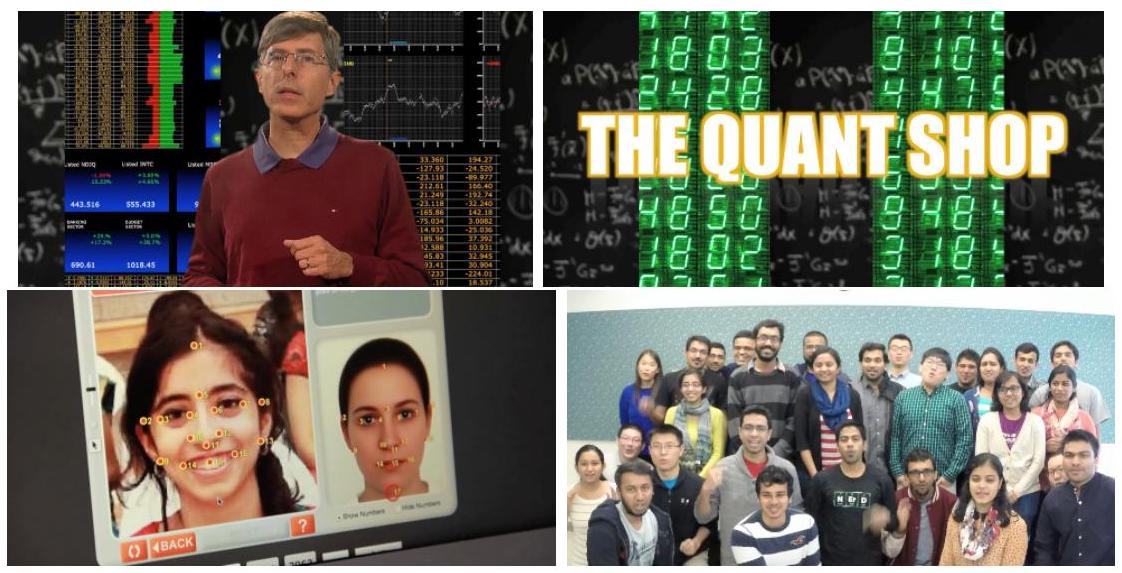
\includegraphics[max width=\textwidth]{2025_03_17_ca60ec0bfd96dcf8e028g-036}
\caption{Exciting scenes from data science television: The Quant Shop.}
\end{figure}

\begin{itemize}
\item \textit{बाज़ार का खेल} - हेज फंड क्वांट्स सही भविष्यवाणी करने पर अमीर बन जाते हैं और गलत होने पर गरीब। सोने और तेल की भविष्य की कीमतों को अतीत की कीमतों के डेटा के माध्यम से हम कितनी सटीकता से पूर्वानुमानित कर सकते हैं? एक सफल मूल्य मॉडल बनाने के लिए और कौन सी जानकारी शामिल होती है? 
\end{itemize}

मैं आपको \textit{The Quant Shop} के कुछ एपिसोड देखने की सलाह देता हूँ, जब आप इस पुस्तक को पढ़ रहे हैं। हम इसे मजेदार बनाने की कोशिश करते हैं, हालांकि मुझे यकीन है कि आपको बहुत सारी चीज़ें अजीब लगेंगी। प्रत्येक शो तीस मिनट तक चलता है और शायद यह आपको अपनी भविष्यवाणी चुनौती से निपटने के लिए प्रेरित करेगा।

ये प्रोग्राम निश्चित रूप से आपको इन आठ विशेष चुनौतियों के बारे में अधिक समझ प्रदान करेंगे। मैं इस पुस्तक में इन प्रोजेक्ट्स का उपयोग महत्वपूर्ण पाठों को दिखाने के लिए करूँगा कि डेटा विज्ञान कैसे किया जाता है, दोनों सकारात्मक और नकारात्मक उदाहरणों के रूप में। ये प्रोजेक्ट्स एक प्रयोगशाला उपलब्ध कराते हैं, जहाँ आप देख सकते हैं कि बुद्धिमान लेकिन अनुभवहीन लोग, जो आपसे बहुत अलग नहीं हैं, ने एक डेटा विज्ञान समस्या के बारे में कैसे सोचा, और जब उन्होंने ऐसा किया तो क्या हुआ।

\subsection{कागल चुनौतियाँ}

एक अन्य प्रेरणा का स्रोत Kaggle (\href{http://www.kaggle.com}{www.kaggle.com}) से चुनौतियाँ हैं, जो डेटा वैज्ञानिकों के लिए एक प्रतिस्पर्धात्मक मंच प्रदान करता है। नियमित रूप से नई चुनौतियाँ पोस्ट की जाती हैं, जो समस्या की परिभाषा, प्रशिक्षण डेटा, और छिपे हुए मूल्यांकन डेटा पर स्कोरिंग फ़ंक्शन प्रदान करती हैं। एक लीडर बोर्ड सबसे मजबूत प्रतिस्पर्धियों के स्कोर को दर्शाता है, जिससे आप देख सकते हैं कि आपका मॉडल आपके प्रतिद्वंद्वियों की तुलना में कितना अच्छा है। विजेता प्रतियोगिता के बाद के साक्षात्कारों में अपने मॉडलिंग रहस्यों को साझा करते हैं, ताकि आप अपनी मॉडलिंग क्षमताओं को सुधार सकें।

Kaggle चुनौतियों में अच्छा प्रदर्शन करना एक उत्कृष्ट साख है जिसे आप अपने फिर से शुरू में शामिल कर सकते हैं ताकि एक अच्छा डेटा वैज्ञानिक के रूप में नौकरी मिल सके। वास्तव में, संभावित नियोक्ता आपको तब ट्रैक करेंगे जब आप एक सच्चे Kaggle स्टार होंगे। लेकिन भाग लेने का असली कारण यह है कि समस्याएं दिलचस्प और प्रेरणादायक होती हैं, और अभ्यास आपको एक बेहतर डेटा वैज्ञानिक बनने में मदद करता है।

प्रत्येक अध्याय के अंत में दिए गए अभ्यास, समाप्त हो चुके Kaggle चुनौतियों की ओर संकेत करते हैं, जो उस अध्याय की सामग्री से ढीले ढंग से जुड़े होते हैं। यह पहले से चेतावनी है कि Kaggle डेटा साइंस का एक भ्रामक आकर्षक दृश्य प्रस्तुत करता है जिसे मशीन लर्निंग के रूप में लागू किया जाता है, क्योंकि यह बहुत ही स्पष्ट रूप से परिभाषित समस्याएँ प्रस्तुत करता है जिनमें डेटा संग्रह और सफाई का मेहनत का काम पहले से ही आपके लिए किया गया होता है। फिर भी, मैं आपको प्रेरणा के लिए इसे देखने के लिए प्रोत्साहित करता हूँ, और नए परियोजनाओं के लिए डेटा के स्रोत के रूप में भी।

\section{युद्ध की कहानियों के बारे में}

असाधारण प्रतिभा और प्रज्ञा दो भिन्न बौद्धिक उपहार हैं। \textit{असाधारण प्रतिभा} सही उत्तर खोजने में प्रकट होती है, कल्पनाशील मानसिक छलांगों में जो बाधाओं और चुनौतियों को पार कर जाती है। \textit{प्रज्ञा} दिखने में तब प्रकट होती है जब हम पहली जगह में बाधाओं से बचते हैं, एक दिशा या मार्गदर्शक प्रकाश प्रदान करते हैं जो हमें सही दिशा में मजबूती से आगे बढ़ने में मदद करता है।

%---- Page End Break Here ---- Page : 19

% Chapter 1: What is Data Science?

प्रतिभा तकनीकी ताकत और गहराई में प्रकट होती है, चीजों को देखने और करने की क्षमता, जो अन्य लोग नहीं कर सकते। इसके विपरीत, ज्ञान अनुभव और सामान्य ज्ञान से आता है। यह दूसरों को सुनने से आता है। ज्ञान विनम्रता से आता है, यह देखने से कि अतीत में आप कितनी बार गलत रहे हैं और यह समझने से कि आप गलत क्यों थे, ताकि भविष्य के जाल को बेहतर ढंग से पहचान सकें और उनसे बच सकें।

डाटा साइंस, जीवन की अधिकतर चीजों की तरह, प्रतिभा की तुलना में अधिक ज्ञान से लाभान्वित होती है। इस बुक में, मैं वह ज्ञान साझा करने की कोशिश कर रहा हूँ जिसे मैंने कठिनाई से \textit{युद्ध की कहानियों} के माध्यम से, उन विभिन्न प्रोजेक्ट्स से सीखा है जिन पर मैंने काम किया है:

\begin{itemize}
  \item \textit{वृहद्-पैमाने पर पाठ विश्लेषण और एनएलपी}: मेरा डेटा विज्ञान प्रयोगशाला स्टॉनी ब्रुक यूनिवर्सिटी में बड़ा डेटा परियोजनाओं पर काम करता है, जिसमें सामाजिक मीडिया से भाव विश्लेषण, ऐतिहासिक प्रवृत्तियों का विश्लेषण, प्राकृतिक भाषा प्रक्रमण (एनएलपी) के लिए गहराई से सीखने के दृष्टिकोण, और नेटवर्क से विशेषता निष्कर्षण शामिल हैं।
  
  \item \textit{स्टार्ट-अप कंपनियाँ}: मैंने जनरल सेंटीमेंट और थ्राइवमेट्रिक्स नामक दो डेटा विश्लेषण कंपनियों के सह-संस्थापक और मुख्य वैज्ञानिक के रूप में सेवा की। जनरल सेंटीमेंट ने लोगों, स्थानों, और चीजों के साथ जुड़े भावनाओं (सकारात्मक या नकारात्मक) में प्रवृत्तियों की पहचान करने के लिए समाचार, ब्लॉग, और सामाजिक मीडिया से वृहद्-पैमाने पर पाठ धाराओं का विश्लेषण किया। थ्राइवमेट्रिक्स ने इस प्रकार के विश्लेषण को ईमेल और मैसेजिंग सिस्टम्स जैसी आंतरिक कॉर्पोरेट संचार पर लागू किया। इन उद्यमों में से कोई भी मुझे इस पुस्तक से मेरे रॉयल्टी को छोड़ने के लिए धनवान नहीं बना पाया, लेकिन उन्होंने मुझे क्लाउड-आधारित कंप्यूटिंग सिस्टम्स पर अनुभव और उद्योग में डेटा के उपयोग की अंतर्दृष्टि प्रदान की।\index{autocorrelation}\index{cicada}\index{fast Fourier transform}\index{FFT}\index{logarithm}
  
  \item \textit{वास्तविक वैज्ञानिकों के साथ सहयोग}: मैंने जीवविज्ञानियों और सामाजिक वैज्ञानिकों के साथ कई रोचक सहयोग किए हैं, जिन्होंने वास्तविक डेटा के साथ काम करने की जटिलताओं की मेरी समझ को आकार दिया। प्रायोगिक डेटा भयंकर रूप से शोरपूर्ण और त्रुटियों से भरा होता है, फिर भी आपको यह पता लगाने के लिए आपके पास जो कुछ भी है उसके साथ सर्वश्रेष्ठ करना होगा कि दुनिया कैसे काम करती है।
  
  \item \textit{जुआ प्रणाली बनाना}: एक विशेष रूप से मनोरंजक परियोजना थी जय-अलाइ मैचों के परिणामों को तीव्र करने के लिए एक प्रणाली बनाना ताकि हम उन पर दांव लगा सकें, जिसका अनुभव मेरी पुस्तक \textit{कैल्कुलेटेड बेट्स: कंप्यूटर, जुआ, और गणितीय मॉडलिंग टू विन} \cite{skiena2001calculated} में वर्णित है। हमारी प्रणाली डेटा संग्रह के लिए वेब स्क्रैपिंग, सांख्यिकीय विश्लेषण, सिमुलेशन/मॉडलिंग, और सावधान मूल्यांकन पर निर्भर थी। हमने सामाजिक मीडिया विश्लेषण का उपयोग कर मूवी ग्रॉस्स, स्टॉक मूल्य, और फुटबॉल खेलों के लिए भविष्यवाणीय मॉडल भी विकसित और मूल्यांकित किए हैं।
  
  \item \textit{ऐतिहासिक हस्तियों का रैंकिंग}: विकिपीडिया का विश्लेषण करके 800,000 से अधिक ऐतिहासिक हस्तियों पर अर्थपूर्ण चर निकालकर, हमने उन्हें ऐतिहासिक मीमों के रूप में उनके शक्ति के द्वारा रैंक करने के लिए एक स्कोरिंग फंक्शन विकसित किया। यह रैंकिंग महानतमों को अन्य सामान्य लोगों से अलग करने में अद्भुत काम करती है (जीसस, नेपोलियन, शेक्सपियर, मोहम्मद, और लिंकन शीर्श पांच में आते हैं) और यह हमारी पुस्तक \textit{व्हूज बिगर?: व्हेयर हिस्टॉरिकल फिगर्स रियली रैंक} \cite{zhang2009improving} के आधार के रूप में कार्य करती है।
\end{itemize}

सारा यह अनुभव इस पुस्तक में जो मैं सिखाता हूँ उसे प्रेरित करता है, विशेष रूप से वे कथाएँ जिन्हें मैं युद्ध कहानियाँ कहता हूँ। \textit{इनमें से हर एक युद्ध कहानी सच्ची है।} बेशक, कहानियाँ पुनः कहने में कुछ हद तक सुधरती हैं, और संवाद को अधिक रोचक बनाने के लिए बनावट प्रदान की गई है। हालाँकि, मैंने सही ढंग से एक खुरदरे समस्या से समाधान तक जाने की प्रक्रिया को ईमानदारी से प्रस्तुत करने का प्रयास किया है, ताकि आप देख सकें कि यह कैसे विकसित हुई।

\section{युद्ध कथा: सही प्रश्न का उत्तर देना}
स्टोनी ब्रुक यूनिवर्सिटी में हमारे अनुसंधान समूह ने एक एनएलपी-आधारित प्रणाली विकसित की है \index{NLP-based system}जो लाखों समाचार, ब्लॉग और सोशल मीडिया संदेशों का विश्लेषण करती है, और इन पाठों को चर्चित सभी संस्थाओं के रुझानों तक सीमित करती है। किसी नाम का पाठ प्रवाह (वॉल्यूम) में ज़िक्र कितनी बार होता है, यह गिनना सिद्धांत रूप में आसान है। यह निर्धारित करना कि किसी विशेष संदर्भ का अर्थ सकारात्मक है या नकारात्मक (भावना विश्लेषण) मुश्किल है। लेकिन हमारी प्रणाली ने यह काम अच्छी तरह से किया, विशेषकर जब इसे कई संदर्भों पर संकलित किया गया।\index{normalizing skewed distribution}

यह तकनीक एक सामाजिक मीडिया विश्लेषण कंपनी जिसका नाम General Sentiment था, के लिए आधार के रूप में कार्य करती थी। एक स्टार्ट-अप की शुरुआत के दौरान उसमें जीना, धन जुटाने, कर्मचारियों की भर्ती करने और नए उत्पाद विकसित करने की चुनौतियों का सामना करना रोमांचक था।

लेकिन शायद सबसे बड़ी समस्या जो हमने झेली वह था सही प्रश्न का उत्तर देना। जनरल सेंटिमेंट प्रणाली ने समाचार, ब्लॉग्स और सामाजिक मीडिया में \textit{हर} व्यक्ति, स्थान, और वस्तु के बारे में भाव और मात्रा के रुझानों को दर्ज किया: 20 मिलियन से अधिक विशिष्ट तत्व। हमने सेलिब्रिटीज और राजनेताओं की प्रतिष्ठा की निगरानी की। हमने कंपनियों और उत्पादों के भाग्य की निगरानी की। हमने खेल टीमों के प्रदर्शन और फिल्मों के बारे में चर्चा को ट्रैक किया। हम कुछ भी कर सकते थे!

लेकिन यह पता चलता है कि कोई भी आपको किसी चीज़ के लिए भुगतान नहीं करता। वे\textit{कुछ} करने के लिए, अपनी किसी विशेष समस्या का समाधान करने के लिए, या अपने व्यवसाय में किसी विशेष दर्द बिंदु को समाप्त करने के लिए भुगतान करते हैं। कुछ भी करने में सक्षम होना एक भयानक विक्रय रणनीति साबित होती है, क्योंकि यह हमसे हर एक ग्राहक के लिए फिर से उस आवश्यकता को खोजने की मांग करती है।

फेसबुक ने सितंबर 2006 तक दुनिया के लिए अपने दरवाजे नहीं खोले थे। इसलिए जब जनरल सेंटिमेंट ने 2008 में शुरुआत की, तो हम सोशल मीडिया युग की बिलकुल शुरुआत में थे। हमारे पास प्रमुख ब्रांडों और विज्ञापन एजेंसियों से बहुत रुचि थी जो \textit{जानती} थीं कि सोशल मीडिया विस्फोट के लिए तैयार था। वे \textit{जानती} थीं कि यह नया मोहक चीज महत्वपूर्ण थी, और उन्हें वहां होना चाहिए। वे \textit{जानती} थीं कि सोशल मीडिया डेटा का सही विश्लेषण उन्हें यह नई समझ दे सकता था कि उनके ग्राहक क्या सोच रहे थे। लेकिन उन्हें वास्तव में यह नहीं पता था कि वे सच में क्या जानना चाहते थे।

एक विमान इंजन निर्माता यह जानने में अत्यधिक रुचि रखता था कि बच्चे फ़ेसबुक पर उनके बारे में कितनी बातें करते हैं। हमें उन्हें धीरे से यह बताना पड़ा कि जवाब शून्य था। अन्य संभावित ग्राहकों ने इस बात के प्रमाण की मांग की कि हम

%---- Page End Break Here ---- Page : 21



थे नीलसन टेलीविजन रेटिंग्स से अधिक सटीक थे। लेकिन बेशक, अगर आप नीलसन रेटिंग्स चाह रहे थे तो आपको उन्हें नीलसन से खरीदना चाहिए। हमारा सिस्टम एक पूरी तरह से अलग दुनिया से विभिन्न अंतर्दृष्टि प्रदान करता था। लेकिन आपको यह जानना आवश्यक था कि आप उनका उपयोग करने के लिए क्या चाहते थे।

हमने विभिन्न प्रकार के ग्राहकों से महत्वपूर्ण अनुबंध प्राप्त करने में सफलता प्राप्त की, जिसमें उपभोक्ता ब्रांड जैसे टयोटा और ब्लैकबेरी, सरकारी संगठन जैसे हवाई पर्यटन कार्यालय, और यहाँ तक कि 2012 में रिपब्लिकन उम्मीदवार मिट रोमनी के राष्ट्रपति अभियान भी शामिल थे। हमारे विश्लेषकों ने उन्हें व्यापार के विविध मुद्दों पर अंतर्दृष्टि प्रदान की:

\begin{itemize}
  \item लोगों ने हवाई के बारे में क्या सोचा? (उत्तर: वे सोचते हैं कि यह घूमने के लिए एक बहुत अच्छी जगह है।)
  \item टोयोटा की भावना गंभीर ब्रेक समस्याओं की खबर के बाद कितनी जल्दी सुधरेगी? (उत्तर: लगभग छह महीने।)
  \item लोगों ने ब्लैकबेरी के नए फोन मॉडलों के बारे में क्या सोचा? (उत्तर: उन्हें iPhone कहीं ज्यादा पसंद आया।)
  \item रोमनी की भावना 47\% मतदाताओं का अपमान करने वाले एक रिकॉर्डेड भाषण के बाद कितनी जल्दी सुधरेगी? (उत्तर: कभी नहीं।)
\end{itemize}

लेकिन प्रत्येक बिक्री के लिए एक नए ब्रह्मांड में प्रवेश करना पड़ता था, जिसमें हमारी बिक्री टीम और शोध विश्लेषकों की ओर से काफी प्रयास और कल्पना शामिल होती थी। हम कभी भी एक ही उद्योग में दो ग्राहक नहीं प्राप्त कर पाए, जिससे हमें पैमाने और संचित ज्ञान का लाभ प्राप्त हो सकता था।

बिल्कुल, ग्राहक हमेशा सही होता है। यह हमारी गलती थी कि हम उन्हें हमारी तकनीक के उपयोग का सबसे अच्छा तरीका नहीं समझा पाए। यहाँ पर सीखा गया सबक यह है कि दुनिया सिर्फ एक नए डेटा स्रोत के लिए आपके दरवाजे पर दस्तक नहीं देगी। आपको डेटा को पैसे में बदलने से पहले सही प्रश्न प्रदान करने में सक्षम होना चाहिए।

\section{अध्याय नोट्स}
बेसबॉल खिलाड़ियों के ऐतिहासिक रिकॉर्ड का उपयोग करके यह स्थापित करने का विचार कि बाएँ हाथ के लोगों की जीवन अवधि छोटी होती है, हैल्पर्न और कोरेन~\cite{halpern1991handedness} के कारण है, लेकिन उनका निष्कर्ष विवादास्पद बना हुआ है। जनसंख्या में बाएँ हाथ के लोगों का प्रतिशत तेजी से बढ़ रहा है, और देखे गए प्रभाव हो सकता है कि सरवाइवरशिप बायस का परिणाम हो~\cite{mcmanus2004right}। तो बाएँ हाथ वालों, लगे रहो! पूरी जानकारी: मैं आप में से एक हूँ।

क्वांटिटेटिव बेसबॉल विश्लेषण के क्षेत्र को कभी-कभी \textit{सेबरमेट्रिक्स} कहा जाता है, और इसके प्रमुख व्यक्ति बिल जेम्स हैं। मैं नवोदित डेटा वैज्ञानिकों को उनकी पुस्तक \textit{हिस्टोरिकल बेसबॉल एब्स्ट्रैक्ट}~\cite{james2010new} पढ़ने की सिफारिश करता हूँ, जो यह बताने का एक उत्कृष्ट उदाहरण है कि कैसे संख्याओं को ज्ञान और समझ में बदला जाता है। \textit{टाइम मैगज़ीन} ने जेम्स के बारे में एक बार कहा: "उन्हें पढ़ने का अधिकांश आनंद इस बात के अप्रतिम दृश्य से आता है कि एक उच्च दर्जे का मस्तिष्क बेसबॉल पर स्वयं को व्यर्थ कर रहा है।" मैं इस पुस्तक में उनकी वेबसाइट की छवियों का उपयोग करने की अनुमति के लिए \href{http://sports-reference.com}{http://sports-reference.com} का धन्यवाद करता हूँ। IMDb के मालिक Amazon के लिए भी यही।

राइड-शेयरिंग प्रणालियों की संभावनाओं का न्यूयॉर्क में अध्ययन Santi et al. \cite{SRS14} द्वारा किया गया था, जिन्होंने दिखाया कि लगभग 95\% यात्राएं पाँच मिनट से अधिक की देरी के बिना साझा की जा सकती थीं।\index{exercises}

लिडिया प्रणाली के लिए भावविश्लेषण \cite{godbole2007large} में वर्णित है। ऐतिहासिक पाठ कॉर्पस जैसे गूगल Ngram के माध्यम से शब्दों के अर्थ में बदलाव की पहचान करने की विधियाँ \cite{kulkarni2015statistically} में रिपोर्ट की गई हैं।

\section{अभ्यास}
\index{exercises}\subsection{डेटा सेट्स की पहचान करना}

\itemपर जाएँ \href{http://data.gov}{http://data.gov}, और पाँच डेटा सेट चुनें जो आपको रुचिकर लगते हैं। प्रत्येक के लिए एक संक्षिप्त विवरण लिखें, और तीन रोचक गतिविधियों का प्रस्ताव दें जो आप उनके साथ कर सकते हैं।
\end{enumerate}

\subsection{प्रश्न पूछना}

\begin{enumerate}
    \item निम्नलिखित डेटा स्रोतों में से प्रत्येक के लिए, तीन रोचक प्रश्न प्रस्तावित करें जिन्हें आप उनका विश्लेषण करके उत्तर दे सकते हैं:
    \begin{itemize}
        \item क्रेडिट कार्ड बिलिंग डेटा।
    \end{itemize}
\end{enumerate}

%---- Page End Break Here ---- Page : 23

\section{कार्यान्वयन परियोजनाएँ}

\begin{enumerate}[resume]
    \item एक प्रोग्राम लिखिए जो एक पुस्तक के बेस्ट-सेलर रैंक को स्क्रैप करे \href{http://Amazon.com}{Amazon.com} पर। इसका उपयोग स्कीना की सभी पुस्तकों के रैंक को समय के साथ प्रदर्शित करने के लिए करें। इनमें से कौन सी पुस्तक अगली वस्तु होनी चाहिए जो आप खरीदें? क्या आपके पास दोस्त हैं जिनके लिए ये एक स्वागत योग्य और उपयुक्त उपहार होगी? :-)
    
    \item आपके पसंदीदा खेल (बेईसबॉल, फुटबॉल, बास्केटबॉल, क्रिकेट, या सॉकर) के लिए, सभी प्रमुख प्रतिभागियों के ऐतिहासिक सांख्यिकीय रिकॉर्ड वाला डेटा सेट पहचानिए। प्रत्येक स्थिति पर सर्वश्रेष्ठ खिलाड़ी की पहचान करने के लिए एक रैंकिंग सिस्टम बनाइए और कार्यान्वित कीजिए।
\end{enumerate}

\section{साक्षात्कार प्रश्न}

\begin{enumerate}[फिर से शुरू करें]
    \item प्रत्येक निम्नलिखित प्रश्नों के लिए: (1) दुनिया की आपकी समझ के आधार पर एक त्वरित अनुमान लगाएं, और फिर (2) एक अधिक सटीक अनुमान प्राप्त करने के लिए Google का उपयोग करें। आपके दोनों अनुमानों में कितना अंतर था?
    \begin{enumerate}
        \item पूरी दुनिया में कितने पियानो ट्यूनर्स हैं?
        \item एक हॉकी रिंक में बर्फ का वजन कितना होता है?
        \item संयुक्त राज्य अमेरिका में कितने गैस स्टेशन हैं?
        \item हर दिन कितने लोग ला गार्डिया एरपोर्ट से आवागमन करते हैं?
        \item संयुक्त राज्य अमेरिका में हर साल कितने गैलन आइस क्रीम बेची जाती है?
        \item नेशनल बास्केटबॉल एसोसिएशन (एनबीए) द्वारा हर साल कितनी बास्केटबॉल खरीदी जाती हैं?
        \item दुनिया के सभी महासागरों में कितनी मछलियाँ हैं?
        \item इस समय पूरी दुनिया में हवा में कितने लोग उड़ रहे हैं?
        \item एक बड़े वाणिज्यिक जेट में कितनी पिंग-पोंग की गेंदें फिट हो सकती हैं?
        \item आपके पसंदीदा देश में कितनी मील पक्की सड़कें हैं?
        \item स्टोनी ब्रूक यूनिवर्सिटी के सभी लोगों की जेबों में कितने डॉलर के बिल हैं?
        \item एक सामान्य गैस स्टेशन प्रति दिन कितने गैलन गैसोलीन बेचता है?
        \item इस किताब में कितने शब्द हैं?
        \item न्यूयॉर्क शहर में कितनी बिल्लियाँ रहती हैं?
        \item स्टारबक्स की कॉफी से एक सामान्य कार की गैस टैंक भरने में कितनी लागत आएगी?
        \item चीन में कितनी चाय है?
        \item संयुक्त राज्य अमेरिका में कितने चेकिंग खाते हैं?
    \end{enumerate}


\itemपुनरावृत्ति और वर्गीकरण के बीच क्या अंतर है?
    
\itemआप डेटा-प्रेरित सिफारिश प्रणाली कैसे बनाएँगे? इस दृष्टिकोण की सीमाएँ क्या हैं?\index{Babbage, Charles}\index{data munging}\index{data science!languages}\index{programming languages}
    
\itemआप डेटा विज्ञान में रुचि कैसे लेने लगे?
    
\itemData विज्ञान को आप कला मानते हैं या विज्ञान?
\end{enumerate}

% Mismatched: \sectionname{Kaggle Challenges}

\begin{enumerate}[फिर से शुरू करें]
\item टाइटैनिक के जहाज के पलटने के हादसे में कौन बचा था? \url{https://www.kaggle.com/c/titanic}

\item एक विशेष टैक्सी कहाँ जा रही है? \url{https://www.kaggle.com/c/pkdd-15-predict-taxi-service-trajectory-i}

\item एक निर्धारित टैक्सी यात्रा में कितना समय लगेगा? \url{https://www.kaggle.com/c/pkdd-15-taxi-trip-time-prediction-ii}
\end{enumerate}

%---- Page End Break Here ---- Page : 25

\chapter{गणितीय प्राथमिकताएँ}
\section{संभाव्यता}
\index{probability}एक डेटा वैज्ञानिक वह व्यक्ति होता है जो एक कंप्यूटर वैज्ञानिक से अधिक सांख्यिकी जानता है और एक सांख्यिकीविद से अधिक कंप्यूटर विज्ञान जानता है।

\begin{quote}
  \textit{जोश ब्लूमनस्टॉक}
\end{quote}

तुम्हें दौड़ने से पहले चलना आना चाहिए। उसी तरह, गणितीय परिपक्वता का एक निश्चित स्तर होता है जो आवश्यक है ताकि आपको संख्यात्मक डेटा के साथ कुछ भी सार्थक करने के लिए भरोसा किया जा सके।

इस पुस्तक को लिखते समय, मैंने यह मान लिया है कि पाठक को प्रायिकता और सांख्यिकी, रैखिक बीजगणित, और सतत गणित का कुछ अनुभव है। मैंने यह भी मान लिया है कि संभवतः उन्होंने इसका अधिकांश भाग भुला दिया होगा, या शायद वे हमेशा पेड़ों के लिए जंगल (चीजें क्यों महत्वपूर्ण हैं और उनका उपयोग कैसे करना है) नहीं देख पाए होंगे (परिभाषाओं, प्रमाणों और संक्रियाओं के सभी विवरण)।

इस अध्याय में हम कुछ बुनियादी गणितीय अवधारणाओं की आपकी समझ को ताज़ा करने का प्रयास करेंगे। मेरे साथ जुड़ें, और यदि आवश्यक हो तो भविष्य के संदर्भ के लिए अपनी पुराने पाठ्यपुस्तकें निकालें। गहरे अवधारणाओं का परिचय पुस्तक में आगे दिया जाएगा जब हमें उनकी आवश्यकता होगी।

\subsection{प्रायिकता के मूलभूत सिद्धांत}
प्रायिकता सिद्धांत घटनाओं की संभावना के बारे में तर्क करने के लिए एक औपचारिक ढांचा प्रदान करता है। क्योंकि यह एक औपचारिक अनुशासन है, इसमें संबद्ध परिभाषाओं का एक जाल होता है जो यह ठीक से निर्धारित करता है कि हम किस पर तर्क कर रहे हैं।



\[ 
  S=\{ (1,1),(1,2),(1,3),(1,4),(1,5),(1,6),(2,1),(2,2),(2,3),(2,4),(2,5),(2,6),
  (3,1),(3,2),(3,3),(3,4),(3,5),(3,6),(4,1),(4,2),(4,3),(4,4),(4,5),(4,6), 
  (5,1),(5,2),(5,3),(5,4),(5,5),(5,6),(6,1),(6,2),(6,3),(6,4),(6,5),(6,6)\} .
  \]
  
  \item An \textit{event} $E$ is a specified subset of the outcomes of an experiment. The event that the sum of the dice equals 7 or 11 (the conditions to win at craps on the first roll) is the subset
  
  \[
  E=\{(1,6),(2,5),(3,4),(4,3),(5,2),(6,1),(5,6),(6,5)\}
  \]

\itemकिसी\textit{संभावना}का परिणाम$s$, दर्शित$p(s)$, दो विशेषताएँ होती हैं:

\begin{itemize}
    \item प्रत्येक परिणाम $s$ में नमूना स्थान $S$, $0 \leq p(s) \leq 1$.
    \item सभी परिणामों की संभावनाओं का योग एक को मिलता है: $\sum_{s \in S} p(s)=1$.
  \end{itemize}


  यदि हम दो विभिन्न निष्पक्ष पासों को मान लें, तो सभी परिणामों $s\timesS$ के लिए संभावना$p(s)=(1 / 6)\in(1 / 6) = 1 / 36$ होती है।

\itemकिसी घटना$E$की संभावना प्रयोग के परिणामों की संभावनाओं का योग होती है। इस प्रकार
  
\[
  p(E)=\sum_{s \in E}p(s)
\]

वैकल्पिक सूत्रीकरण घटना के \textit{पूरक} के संदर्भ में है $\bar{E}$, वह स्थिति जब $E$ घटित नहीं होता है। तब

\[
  P(E)=1-P(\bar{E}) .
  \]

यह उपयोगी है, क्योंकि अक्सर$P(\bar{E})$का विश्लेषण करना सीधे$P(E)$से आसान होता है।

\itemA\textit{यादृच्छिक चर}$V$संभावना स्पेस के परिणामों पर एक संख्यात्मक फ़ंक्शन होता है। फ़ंक्शन "दो पासों के मानों का योग करें"$(V((a, b))=a+b)$2 और 12 के बीच एक पूर्णांक परिणाम उत्पन्न करता है। यह यादृच्छिक चर के मानों के संभावना वितरण को दर्शाता है। संभावना$P(V(s)=7)=1 / 6$, जैसा कि पहले दिखाया गया था, जबकि$P(V(s)=12)=1 / 36$।\index{C–language}\index{Excel}\index{Java}\index{Mathematica}\index{notebook environments}\index{Wolfram Alpha}

\itemएक\textit{यादृच्छिक चर}का अपेक्षित मान$V$जो एक सैंपल स्पेस$S$पर परिभाषित है,$E(V)$ के रूप में परिभाषित है
  
\[
  E(V)=\sum_{s \in S}p(s)\cdotV(s)
\]

\end{itemize}

यह सब आप पहले से ही देख चुके होंगे। लेकिन यह वह भाषा प्रदान करता है जिसे हम प्रॉबेबिलिटी और स्टैटिस्टिक्स के बीच जोड़ने के लिए उपयोग करेंगे। जो डेटा हम देखते हैं वह आमतौर पर देखे गए घटनाओं की विशेषताओं को मापने से आता है। प्रॉबेबिलिटी और स्टैटिस्टिक्स का सिद्धांत इस डेटा का विश्लेषण करने के लिए उपकरण प्रदान करता है।

\subsection{प्रायिकता बनाम सांख्यिकी}
प्रायिकता और सांख्यिकी गणित के संबंधित क्षेत्र हैं जो घटनाओं की सापेक्षिक आवृत्ति के विश्लेषण से संबंधित होते हैं। फिर भी, वे दुनिया को देखने के तरीके में मौलिक अंतर होते हैं:

\begin{itemize}
  \item \textit{प्रायिकता} भविष्य की घटनाओं की संभावनाओं का पूर्वानुमान लगाने से संबंधित है, जबकि \textit{सांख्यिकी} पूर्व की घटनाओं की आवृत्ति के विश्लेषण से संबंधित है।
  \item प्रायिकता मुख्य रूप से गणित की एक सैद्धांतिक शाखा है, जो गणितीय परिभाषाओं के परिणामों का अध्ययन करती है। सांख्यिकी मुख्य रूप से गणित की एक अनुप्रयुक्त शाखा है, जो वास्तविक दुनिया में देखी गई चीजों को समझने की कोशिश करती है।\index{CSV files}\index{XML}
\end{itemize}

दोनों विषय महत्वपूर्ण, प्रासंगिक, और उपयोगी हैं। लेकिन वे भिन्न हैं, और गणितीय प्रमाण की प्रासंगिकता को सही रूप में समझने के लिए यह भेद जानना महत्वपूर्ण है। कई जुआरी एक ठंडी और अकेली कब्र में चले गए हैं क्योंकि उन्होंने संभावना और सांख्यिकी के बीच उचित भेद नहीं किया।

यह भेद संभवतः स्पष्ट हो जाएगा यदि हम एक गणितज्ञ के विचार प्रक्रिया का अनुसरण करें जब वह पहली बार एक craps गेम का सामना करती है:

\begin{itemize}
  \item यदि यह गणितज्ञ एक प्रायोगिक चिकित्सक होती, तो वह पासे देखती और सोचती "छः-पक्षीय पासा? प्रत्येक पक्ष के समान रूप से सामने आने की संभावना है। अब मान लेते हैं कि प्रत्येक पक्ष की संभावना $1 / 6$ है, तो मैं यह पता लगा सकती हूं कि मेरे हारने की कितनी संभावना है।"
  \item यदि इसके बजाय एक सांख्यिकीविद उधर से गुजरें, तो वह पासे देखतीं और सोचतीं "मुझे कैसे पता चलेगा कि इसे छेड़ा नहीं गया है? मैं कुछ देर देखती रहूंगी, और ध्यान रखूंगी कि हर संख्या कितनी बार आती है। तब मैं निर्णय कर सकती हूं कि मेरे अवलोकन समान-संभाव्यता वाले पक्षों के अनुमान के अनुरूप हैं या नहीं। एक बार जब मैं इस बात को लेकर आश्वस्त हो जाऊंगी कि पासा निष्पक्ष है, तो मैं किसी प्रायोगिक चिकित्सक को बुलाऊंगी जो मुझे बता सके कि दांव कैसे लगाना है।"
\end{itemize}

सारांश में, प्रायिकता सिद्धांत हमें एक आदर्श दुनिया के परिणामों को खोजने में सक्षम बनाता है, जबकि सांख्यिकी सिद्धांत हमें इस बात को मापने में सक्षम बनाता है कि हमारी दुनिया कितनी आदर्श है। सिद्धांत और व्यवहार के बीच यह निरंतर तनाव ही वह कारण है जिसके कारण सांख्यिकीविद आशावादी प्रायिकताविदों की तुलना में दुखी रहने वाले होते हैं।

आधुनिक संभावना सिद्धांत पहली बार 1654 में फ्रांस के पासे की टेबलों में उभरा। शेवालियर डे मेरी, एक फ्रांसीसी कुलीन, सोच रहे थे कि एक विशेष सट्टेबाजी खेल में खिलाड़ी के पास या हाउस के पास फायदा था। \footnote{वास्तव में उसे ऐसा नहीं सोचना चाहिए था। हाउस के पास हमेशा फायदा होता है।} मूल संस्करण में, खिलाड़ी चार पासे फेंकता है, और जीत तब होती है जब उनमें से कोई भी 6 नहीं होता। अगर कम से कम एक 6 आता है, तो हाउस बराबर पैसे की शर्त पर जीत जाता है।

डे मेरे ने इस समस्या को फ्रांसीसी गणितज्ञ ब्लेज़ पास्कल और पियर डे फर्मा के ध्यान में लाया, जो सबसे प्रसिद्ध फर्मा का अंतिम प्रमेय के स्रोत के रूप में जाने जाते हैं। साथ मिलकर, इन लोगों ने संभाव्यता सिद्धांत की बुनियादी बातें विकसित कीं, इस प्रक्रिया में यह स्थापित किया कि हाउस इस पासा खेल में संभाव्यता$p=1-(5 / 6)^4\approx0.517$के साथ जीतता है, जहां संभाव्यता$p=0.5$एक निष्पक्ष खेल को दर्शाता है जहां हाउस बिल्कुल आधे समय पर जीतता है।

\subsection{संयोजित घटनाएँ और स्वतंत्रता}
हम सरल घटनाओं$A$और$B$से गणना की गई जटिल घटनाओं में रुचि लेंगे, जो परिणामों के उसी सेट पर होते हैं। संभवतः घटना$A$इस बात को इंगित करती है कि कम से कम दो पासे में से एक सम संख्या हो, जबकि घटना$B$समग्र रूप से या तो 7 या 11 का अंक प्राप्त करना है। ध्यान दें कि$A$के कुछ परिणाम मौजूद हैं जो$B$के परिणाम नहीं हैं, विशेषकर

\[\]

\begin{aligned}
A-B=\{ & (1,2),(1,4),(2,1),(2,2),(2,3),(2,4),(2,6),(3,2),(3,6),(4,1) \\\index{AOL}\index{company data}\index{data!collecting}\index{data sources}\index{protocol buffers}
& (4,2),(4,4),(4,5),(4,6),(5,4),(6,2),(6,3),(6,4),(6,6)\}
\end{aligned}

\]

यह सेट डिफरेंस ऑपरेशन है। ध्यान दें कि {यहाँ}$B-A=\⸨\⸩$ है, क्योंकि 7 या 11 बनाने वाले प्रत्येक युग्म में एक विषम और एक सम संख्या होनी चाहिए।

दोनों घटनाओं$A$और$B$के बीच सामान्य परिणामों को इंटरसेक्शन कहा जाता है, जिसे$A\capB$द्वारा इंगित किया जाता है। इसे इस प्रकार लिखा जा सकता है

\[ 
A \cap B=A-(S-B) .
\]

ऐसे परिणाम जो या तो$A$या$B$में दिखाई देते हैं, उन्हें यूनियन कहा जाता है, और इसे $A\cupB$ द्वारा अंकित किया जाता है। पूरक ऑपरेशन के साथ $\bar{A}=S-A$, हमें घटनाओं को जोड़ने के लिए एक समृद्ध भाषा मिलती है, जैसा कि चित्र 2.1 में दिखाया गया है। हम परिभाषित सेटों में परिणामों की संख्याओं को जोड़कर इन सेटों की संभावना आसानी से गणना कर सकते हैं।

घटनाएँ$A$और$B$स्वतंत्र होती हैं यदि और केवल यदि

\[ 
P(A \cap B)=P(A) \times P(B)
\]

इसका अर्थ यह है कि घटनाओं $A$ और $B$ के बीच परिणामों की कोई विशेष संरचना साझा नहीं की जाती है। यह मानते हुए कि मेरी कक्षा में आधी छात्राएं महिला हैं, और आधे छात्र मेरी कक्षा में औसत से ऊपर हैं, हम उम्मीद करेंगे कि मेरी कक्षा में एक चौथाई छात्राएं दोनों महिला और औसत से ऊपर हैं यदि घटनाएं स्वतंत्र हैं।

\begin{figure}[h]
  \centering
  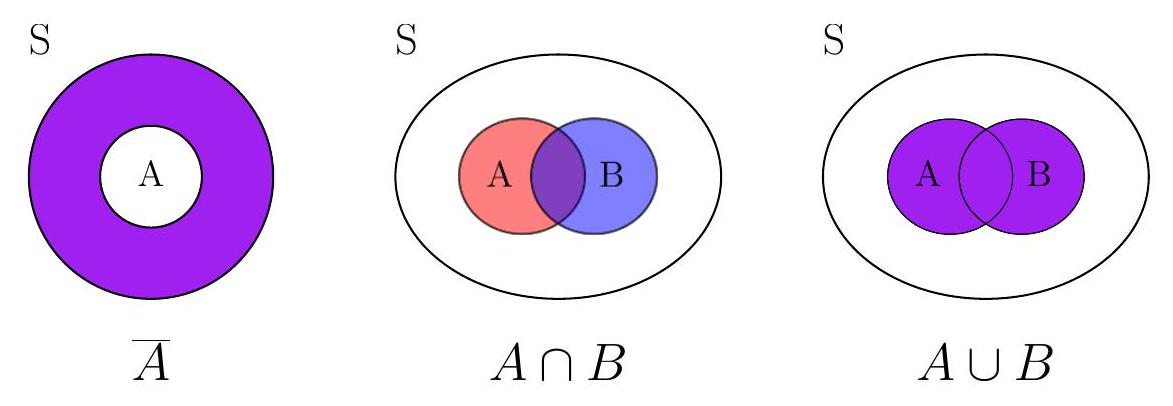
\includegraphics[max width=\textwidth]{2025_03_17_ca60ec0bfd96dcf8e028g-047}
  \caption{Venn diagrams illustrating set difference (left), intersection (middle), and union (right).}
\end{figure}

%---- Page End Break Here ---- Page : 30



प्रायिकता के सिद्धांतकार स्वतंत्र घटनाओं को पसंद करते हैं, क्योंकि यह उनके गणनाओं को सरल बनाता है। लेकिन डेटा वैज्ञानिक सामान्यतः ऐसा नहीं करते। जब हम किसी भविष्य की घटना$B$ की संभावना का पूर्वानुमान लगाने के लिए मॉडल बना रहे होते हैं, यह जानते हुए कि कोई पिछली घटना$A$ हो चुकी है, तो हम चाहते हैं कि$B$का$A$पर यथासंभव मजबूत निर्भरता हो।

मान लीजिए कि मैं हमेशा छतरी का उपयोग करता हूँ, यदि और केवल यदि बारिश हो रही हो। मान लीजिए कि यहाँ बारिश होने की संभावना (घटना$B$) है, मान लीजिए,$p=1/5$। इसका तात्पर्य है कि मैं अपनी छतरी ले जा रहा हूँ की संभावना (घटना$A$) है$q=1/5$। लेकिन इससे भी अधिक, अगर आपको बारिश की स्थिति का पता है, तो आप यह भी सटीक रूप से जानते हैं कि मेरे पास मेरी छतरी है या नहीं। ये दो घटनाएँ पूरी तरह से\textit{सहसंबद्ध}हैं।

इसके विपरीत, कल्पना करें कि घटनाएँ स्वतंत्र थीं। तब

\[
P(A \mid B)=\frac{P(A \cap B)}{P(B)}=\frac{P(A) P(B)}{P(B)}=P(A)
\]

और यह बारिश हो रही है या नहीं इसका मेरे सुरक्षात्मक गियर ले जाने पर बिल्कुल भी प्रभाव नहीं पड़ता।

संबंध भविष्यवाणी मॉडल के पीछे की प्रेरक शक्ति हैं, इसलिए हम उन्हें मापने के तरीके और उनका क्या अर्थ है, इस पर चर्चा सेक्शन 2.3 में करेंगे।

\subsection{सशर्त संभावना}
जब दो घटनाएं सहसंबद्ध होती हैं, तो उनके बीच एक निर्भरता होती है जो गणनाओं को अधिक कठिन बना देती है। \textit{सशर्त संभावना} A का, जब B दिया गया हो, P(A$B) इस प्रकार परिभाषित है:\index{academic data}\index{Google Scholar}\index{sweat equity}

\[
P(A \mid B)=\frac{P(A \cap B)}{P(B)}
\]

अनुभाग 2.1.2 के पासा फेंकने की घटनाओं को याद करें, अर्थात्:

\begin{itemize}
  \item घटना $A$ यह है कि कम से कम एक पासे की संख्या सम हो।
  \item घटना $B$ यह है कि दोनों पासों का योग या तो 7 है या 11।
\end{itemize}

ध्यान दें कि$P(A\midB)=1$, क्योंकि कोई भी रोल जिससे विषम मान प्राप्त होता है, उसे एक सम और एक विषम संख्या का ही योग होना चाहिए। इस प्रकार$A\capB=B$, जैसे कि ऊपर दिए गए छतरी के मामले में। $P(B\midA)$ के लिए, ध्यान दें कि$P(A\capB)=9/36$ और$P(A)=25/36$, इसलिए$P(B\midA)=9/25$।

सशर्त प्रायिकता हमारे लिए महत्वपूर्ण होगी, क्योंकि हम किसी घटना$A$ (संभवतः कि ईमेल का कोई विशेष अंश स्पैम है) की संभावना में रुचि रखते हैं, जो कि कुछ सबूत$B$ (संभवतः दस्तावेज़ के अंदर शब्दों का वितरण) के रूप में होती है। वर्गीकरण की समस्याएँ सामान्यतः किसी न किसी तरीके से सशर्त प्रायिकताओं की गणना करना ही होता है।

हमारा प्रमुख उपकरण सशर्त संभावनाओं की गणना करने के लिए बेयेस प्रमेय होगा, जो निर्भरताओं की दिशा को उलट देता है:

\[
P(B \mid A)=\frac{P(A \mid B) P(B)}{P(A)}
\]

अक्सर यह एक दिशा में संभावनाएँ गणना करना दूसरी दिशा की अपेक्षा आसान साबित होता है, जैसे कि इस समस्या में. बेज़ प्रमेय$P(B\midA)= (1\cdot9/36)/(25/36) = 9/25$, बिल्कुल 
वही जो हम पहले प्राप्त कर चुके हैं. हम बेज़ प्रमेय को अनुभाग 5.6 में फिर से देखेंगे, जहाँ यह प्रमाणों के आधार पर संभावनाएँ गणना करने की नींव स्थापित करेगा.

\subsection{प्रायिकता वितरण}
\index{probability distribution}यादृच्छिक चरों में संख्यात्मक कार्य होते हैं जहाँ मान विशिष्ट घटनाओं की प्रायिकता से जुड़े होते हैं। हमारे उदाहरण में जहाँ$V(s)$दो फेंके गए पासों का योग है, यह कार्य 2 और 12 के बीच के पूर्णांक का उत्पादन करता है। किसी विशेष मान की प्रायिकता$V(s)=X$सभी परिणामों की प्रायिकताओं का योग है जो मिलकर$X$बनते हैं।

ऐसे यादृच्छिक चर को उनके \textit{प्रायिकता घनत्व फलन}, या पीडीएफ द्वारा प्रदर्शित किया जा सकता है। यह एक ग्राफ होता है जहाँ $x$-अक्ष यादृच्छिक चर के लिए मानों की सीमा को प्रदर्शित करता है, और $y$-अक्ष उस दिए गए मान की प्रायिकता को दर्शाता है। चित्र~\ref{fig:pdf-cdf} (बायाँ) दो निष्पक्ष पासों के योग का पीडीएफ प्रस्तुत करता है। ध्यान दें कि $X=7$ पर शिखर सबसे अधिक बार आने वाले पासे योग के अनुरूप है, जिसमें $1/6$ की प्रायिकता है।

ऐसे पीडीएफ प्लॉट्स का डेटा फ्रीक्वेंसी के हिस्टोग्राम से एक मजबूत संबंध होता है, जहाँ पर $x$-एक्सिस फिर से मान की श्रृंखला का प्रतिनिधित्व करता है, लेकिन $y$ अब यह दर्शाता है कि दिए गए प्रत्येक मान $X$ के लिए कितनी बार घटना की घटनाएँ देखी गईं। हिस्टोग्राम को पीडीएफ में बदलने के लिए प्रत्येक बकेट को सभी बकेट्स की कुल फ्रीक्वेंसी से भाग दिया जा सकता है। तब प्रविष्टियों का योगफल 1 हो जाता है, जिससे हमें एक प्रायिकता वितरण प्राप्त होता है।

Histogram सांख्यिकीय होते हैं: वे परिणामों के वास्तविक प्रेक्षणों को दर्शाते हैं। इसके विपरीत, पीडीएफ प्रायिक होते हैं: वे यह प्रतिनिधित्व करते हैं कि अगला प्रेक्षण किस संभावना से मान$X$हो सकता है। हम अक्सर प्रेक्षणों का हिस्टोग्राम $h(x)$ व्यवहार में प्रायिकताओं का अनुमान लगाने के लिए उपयोग करते हैं\footnote{एक तकनीक जिसे डिस्काउंटिंग कहा जाता है दुर्लभ घटनाओं की आवृत्ति का बेहतर अनुमान लगाने का तरीका प्रदान करती है, और इसे अनुभाग~\ref{sec:discounting}में चर्चा की जाएगी।}कुल प्रेक्षणों की संख्या से गिनती को सामान्यीकृत करके:\index{Aaron Schwartz case}\index{data!logging}\index{Internet of Things}\index{terms of service}\index{web crawling}

\[
P(k=X)=\frac{h(k=X)}{\sum_{x} h(x=X)}
\]

एक अन्य तरीका है जिससे यादृच्छिक चर को प्रदर्शित किया जा सकता है, जिसे अक्सर उपयोगी पाया जाता है, इसे \textit{संचयी सघनता फलन} या cdf कहा जाता है। cdf पीडीएफ़ में संभावनाओं का संचयी योग है; $k$ का फलन होने के कारण, यह दर्शाता है कि $X\leqk$ की संभावना है बजाय इसके कि $X=k$ की। चित्र~\ref{fig:pdf-cdf} (दाईं ओर) पासे के योग वितरण का cdf दर्शाता है। मान बाईं से दाईं ओर एकरूपी रूप से बढ़ते जाते हैं, क्योंकि प्रत्येक पद का योगदान पिछले कुल में धनात्मक संभावना जोड़कर होता है। सबसे दाईं ओर का मान 1 होता है, क्योंकि सभी परिणाम अधिकतम से बड़ा मूल्य उत्पन्न नहीं करते।

यह समझना महत्वपूर्ण है कि ⸨pdf$P(V)⸩ और ⸨cdf$C(V)⸩ एक दिए गए यादृच्छिक चर$V$ की एक समान जानकारी रखते हैं। हम इनके बीच आसानी से स्थानांतरित कर सकते हैं क्योंकि:

\[
P(k=X)=C(X \leq k+\delta)-C(X \leq k)
\]

जहाँ $\delta=1$ पूर्णांक वितरणों के लिए। सीडीऍफ पीडीऍफ का चलित योग है, इसलिए

\[
C(X \leq k)=\sum_{x \leq k} P(X=x)
\]

बस यह सुनिश्चित करें कि आप किस वितरण को देख रहे हैं। संचयी वितरण हमेशा दाएँ जाने पर अधिक हो जाते हैं, और यह एक संभावना में उच्चतम बिंदु पर पहुँचता है जिससे$C(X\leq\infty)=1$। इसके विपरीत, एक पीडीएफ के वक्र के नीचे का कुल क्षेत्रफल 1 के बराबर होता है, इसलिए वितरण के किसी भी बिंदु पर संभावना सामान्यतः काफी कम होती है।

\begin{figure}[h!]
    \centering
    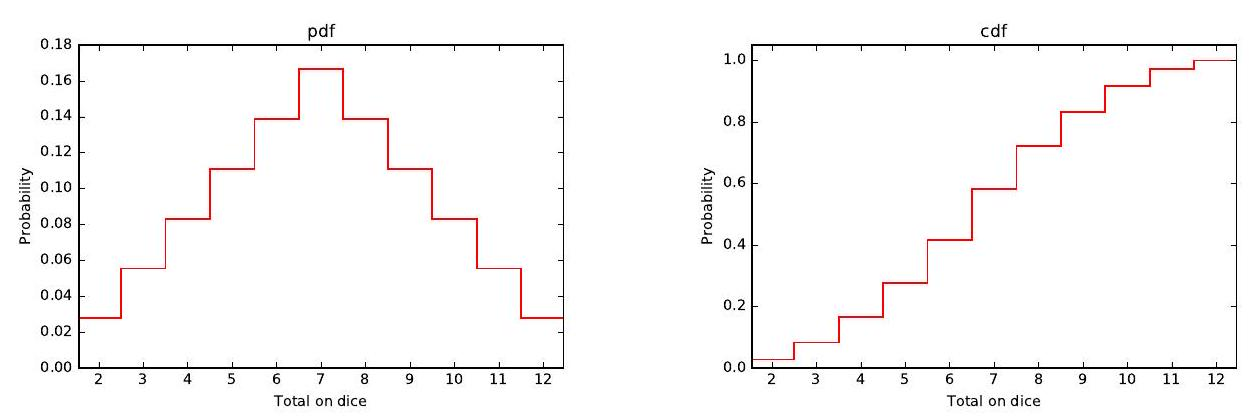
\includegraphics[max width=\textwidth]{2025_03_17_ca60ec0bfd96dcf8e028g-049}
    \caption{The probability density function (pdf) of the sum of two dice contains exactly the same information as the cumulative density function (cdf), but looks very different.}
    \label{fig:pdf-cdf}
\end{figure}

Apple आईफोन बिक्री के लिए संचयी और वृद्धिशील वितरण के बीच के अंतर का एक मनोरंजक उदाहरण चित्र~\ref{fig:iphone-sales} में दिखाया गया है। दोनों वितरण Apple आईफोन बिक्री पर बिल्कुल समान डेटा दिखाते हैं, लेकिन Apple के सीईओ टिम कुक ने एक प्रमुख शेयरधारक कार्यक्रम में कौन सा ग्राफ प्रस्तुत करने के लिए चुना? संचयी वितरण (लाल) दिखाता है कि बिक्री तेजी से बढ़ रही है, है ना? लेकिन यह वृद्धि दर का एक भ्रामक दृश्य प्रस्तुत करता है, क्योंकि वृद्धिशील परिवर्तन इस फ़ंक्शन का व्युत्पन्न है, और इसे देखना मुश्किल है। वास्तव में, प्रति-तिमाही बिक्री ग्राफ (नीला) दिखाता है कि प्रस्तुति से पहले की अंतिम दो अवधियों में आईफोन बिक्री दर वास्तव में घट गई थी।

\begin{figure}[h!]
    \centering
    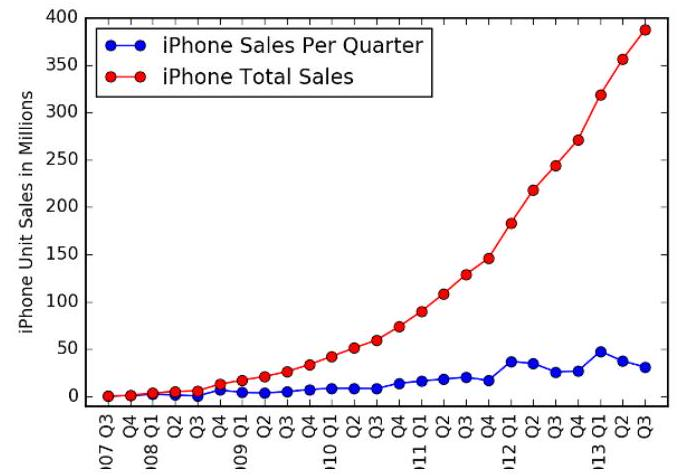
\includegraphics[max width=\textwidth]{2025_03_17_ca60ec0bfd96dcf8e028g-050}
    \caption{iPhone quarterly sales data presented as cumulative and incremental (quarterly) distributions. Which curve did Apple CEO Tim Cook choose to present?}
    \label{fig:iphone-sales}
\end{figure}

\section{वर्णनात्मक सांख्यिकी}
वर्णनात्मक सांख्यिकी एक दिए गए डेटा सेट या नमूने के गुणों को पकड़ने के तरीके प्रदान करती है। वे देखे गए डेटा का सारांश देती हैं और इसके बारे में बात करने के लिए एक भाषा प्रदान करती हैं। औसत, न्यूनतम, गणना या योग जैसे एक नए व्युत्पन्न तत्व द्वारा तत्वों के एक समूह का प्रतिनिधित्व करना एक बड़े डेटा सेट को एक छोटे सारांश सांख्यिकी में बदल देता है: डेटा कमी के रूप में संकलन।\index{Pubmed}

ऐसी सांख्यिकी अपने आप में विशेषताएँ बन सकती हैं जब उन्हें पूरे डेटा सेट में प्राकृतिक समूहों या समूहों पर लिया जाता है। वर्णनात्मक सांख्यिकी के दो मुख्य प्रकार होते हैं:

\begin{itemize}
  \item \textit{केन्द्र प्रवृत्ति के उपाय}, जो उस केन्द्र को दर्शाते हैं जिसके चारों ओर डेटा वितरित होता है।
  \item \textit{प्रसरण} या \textit{विविधता के उपाय}, जो डेटा के प्रसार का वर्णन करते हैं, अर्थात माप केन्द्र से कितनी दूर स्थित हैं।
\end{itemize}

इन सांख्यिकी ने मिलकर हमें हमारे वितरण के बारे में अत्यधिक जानकारी प्रदान की है।

\subsection{केंद्रीयता मापदंड}
आँकड़ों का पहला तत्व जिसे हम स्कूल में जानते हैं, वे हैं मूल केंद्रीयता मापदंड: औसत, माध्यिका, और वारंम्यता । जब किसी डेटा सेट को एक संख्या से वर्णन करने की बात आती है, तो ये आरंभ करने के लिए सही स्थान हैं।

\begin{itemize}
  \item \textit{औसत}: आप शायद \textit{गणितीय औसत} के उपयोग के साथ काफी सहज महसूस करते हैं, जहाँ हम मूल्यों को जोड़ते हैं और अवलोकनों की संख्या से विभाजित करते हैं:
\end{itemize}

\[
\mu_{X}=\frac{1}{n} \sum_{i=1}^{n} x_{i}
\]

हम आसानी से प्रविष्टियों और विलोपनों की धारा के तहत माध्य को बनाए रख सकते हैं, मूल्य के योग को आवृत्ति गिनती से अलग रखते हुए, और केवल मांग पर विभाजित करते हैं। माध्य बहुत अर्थपूर्ण होता है सममित वितरणों को चित्रित करने के लिए जिसमें बाह्यांक नहीं होते, जैसे कि ऊँचाई और वजन। इसका सममित होने का अर्थ है कि माध्य से ऊपर वस्तुओं की संख्या भूमिकायमान होनी चाहिए जितनी कि संख्या

%---- Page End Break Here ---- Page : 34



यह कि यह बाह्य मानों के बिना है, इसका अर्थ है कि मानों की श्रेणी यथोचित रूप से संकुचित है। ध्यान दें कि एक अकेला MAXINT, जो आमतौर पर सही पर्यवेक्षनों के समूह में आ जाता है, औसत को बुरी तरह से प्रभावित करता है। माध्यिका एक केंद्रीयता माप है जो ऐसी अव्यवस्थित वितरणों के लिए अधिक उपयुक्त साबित होती है।\index{data!compatibility}\index{unit conversions}

\subsubsection{ज्यामितीय माध्य}

The\emph{ज्यामितीय माध्य}$n$मूल है $n$मानों के गुणनफल का:

$$
\left(\prod_{i=1}^{n}a_{i}\right)^{1 / n}=\sqrt[n]{a_{1} a_{2} \ldots a_{n}}
$$

ज्यामितीय औसत हमेशा अंकगणितीय औसत से कम या उसके बराबर होता है। उदाहरण के लिए, 36 पासों के रोल के योग का ज्यामितीय औसत 6.5201 है, जबकि अंकगणितीय औसत 7 है। यह शून्य के करीब के मानों के प्रति बहुत संवेदनशील होता है। शून्य का एक अकेला मान ज्यामितीय औसत को बेकार कर देता है: आपके डेटा में चाहे जितने भी अन्य मान हों, आप अंत में शून्य पाते हैं। यह कुछ हद तक उस स्थिति के समान है जब अंकगणितीय औसत में$\infty$एक अपवाद होता है। लेकिन जब अनुपातों का औसत निकालने की बात आती है तब ज्यामितीय औसत अपनी उपयोगिता साबित करता है।$1 / 2$और$2 / 1$का ज्यामितीय औसत 1 है, जबकि औसत 1.25 है। 1 से कम अनुपातों के लिए उपलब्ध "स्थान" 1 से अधिक अनुपातों के लिए उपलब्ध स्थान की तुलना में कम होता है, जिससे असममितता पैदा होती है जिसे अंकगणितीय औसत बढ़ा-चढ़ाकर दिखा देता है। इन मामलों में ज्यामितीय औसत अधिक सार्थक होता है, जैसे कि अनुपातों के\emph{लघुगणक}के अंकगणितीय औसत की तरह।

\subsubsection{मध्यिका}

माध्यिका एक डेटा सेट में बिलकुल मध्य मूल्य होती है; जितने तत्व माध्यिका के \emph{ऊपर} होते हैं, उतने ही उसके ⸨नीचे⸩ होते हैं। जब आपके पास तत्वों की संख्या सम होती है, तो माध्यिका के बारे में एक छोटी सी बहस होती है कि किसे लिया जाए। आप दो केंद्रीय उम्मीदवारों में से किसी एक को ले सकते हैं: किसी भी संगत डेटा सेट में ये दोनों मूल्य लगभग समान होने चाहिए। वास्तव में, पासे के उदाहरण में, दोनों ही 7 हैं।

माध्यिका की इस तरह से परिभाषित की गई एक अच्छी विशेषता यह है कि यह मूल डेटा धारा का वास्तविक मान होना चाहिए। वास्तव में, आप उस व्यक्ति को उदाहरण के रूप में दिखा सकते हैं जो आपकी माध्यिका ऊँचाई का है, लेकिन शायद दुनिया में कोई व्यक्ति \emph{सटीक} औसत ऊँचाई का नहीं है। आप यह विशेषता तब खो देते हैं जब आप दो केंद्र तत्वों का औसत निकालते हैं।

कौन सा केंद्रीयता माप अनुप्रयोगों के लिए सबसे अच्छा है? माध्यमिक सामान्यतः सममित वितरणों में अंकगणितीय माध्य के काफी करीब होता है, लेकिन यह देखना अक्सर रोचक होता है कि वे कितनी दूर हैं, और माध्य के किस तरफ माध्यमिक स्थित है।

माध्यिका आमतौर पर टेढ़ी विरटनाओं या ऐसे डेटा के लिए बेहतर सांख्यिकीय प्रमाणित होती है जिसमें बाह्यांक होते हैं: जैसे धन और आय। बिल गेट्स संयुक्त राज्य अमेरिका में व्यक्ति पर आधारिक औसत धन में\$250 जोड़ते हैं, लेकिन मध्यिका में कुछ नहीं जोड़ते। अगर वो आपको व्यक्तिगत रूप से अधिक धनी महसूस कराते हैं, तो आगे बढ़िए और औसत का उपयोग कीजिए। लेकिन यहाँ पर मध्यिका अधिक सूचनात्मक सांख्यिकीय होती है, जैसे कि यह किसी भी पावर लॉ वितरण के लिए होगी।



\subsubsection{मोड}
\index{mode}
\emph{मोड} डेटा सेट में सबसे बार-बार आने वाला तत्व होता है। हमारे जारी पासा उदाहरण में, यह 7 है, क्योंकि यह छत्तीस तत्वों में से छह बार आता है। सच कहूँ, तो मैंने कभी भी ⸨मोड⸩ को केंद्रीयता माप के रूप में बहुत अधिक अंतर्दृष्टि प्रदान करते हुए नहीं देखा है, क्योंकि यह अक्सर केंद्र के करीब नहीं होता है। किसी बड़े रेंज पर मापे गए नमूनों में बहुत कम दोहराए गए तत्व या किसी विशेष मूल्य पर टकराव होते हैं। इससे ⸨मोड⸩ एक संयोग की बात बन जाता है। वास्तव में, अक्सर बार-बार आने वाले तत्व डेटा सेट में कलाकृतियों या विसंगतियों को प्रकट करते हैं, जैसे कि डिफ़ॉल्ट मान या त्रुटि कोड जो वास्तव में अंतर्निहित वितरण के तत्वों को प्रस्तुत नहीं करते हैं। आवृत्ति वितरण (या हिस्टोग्राम) में प्रमुखता की संबंधित अवधारणा अर्थपूर्ण होती है, लेकिन दिलचस्प प्रमुखताएँ केवल उचित बकेटिंग के माध्यम से ही प्रकट होती हैं। संयुक्त राज्य अमेरिका में वार्षिक वेतन वितरण की वर्तमान प्रमुखता\$30,000 और\$40,000 प्रति वर्ष के बीच में है, यद्यपि ⸨मोड⸩ निश्चिततः शून्य पर बैठा होता है।\index{character code unification}\index{name unification}\index{numerical conversions}

\subsection{वैरिएबिलिटी माप}
\index{variability measures}
सबसे सामान्य वैरिएबिलिटी माप \emph{मानक विचलन}\index{standard deviation}$\sigma$ होता है, जो व्यक्तिगत तत्वों और औसत के बीच वर्गों के अंतर के योग को मापता है:

$$
\sigma=\sqrt{\frac{\sum_{i=1}^{n}\left(a_{i}-\bar{a}\right)^{2}}{n-1}}
$$

एक संबंधित सांख्यकीय तथ्य, \emph{वैरियंस}$V$, मानक विचलन का वर्ग होता है, अर्थात् $V=\sigma^{2}$। कभी-कभी वैरियंस के बारे में बात करना अधिक सुविधाजनक होता है क्योंकि यह शब्द मानक विचलन की तुलना में आठ अक्षर छोटा होता है। लेकिन वे बिल्कुल वही चीज़ मापते हैं।

उदाहरण के लिए, साधारण बल्ब को देखें, जो आमतौर पर अपेक्षित कार्यकाल के साथ आता है, मान लें कि$\mu=3000$घंटे, जो फिगर 2.4 में दिखाए गए कुछ आधारभूत वितरण से लिया गया है। एक पारंपरिक बल्ब में, उसके लंबे समय तक चलने की संभावना$\mu$उसे जल्दी जलने की संभावना के लगभग बराबर होती है, और इस अनिश्चितता के स्तर को$\sigma$द्वारा मापा जाता है। वैकल्पिक रूप से, एक "प्रिंटर\ldots

%---- Page End Break Here ---- Page : 36





कार्ट्रिज बल्ब," जहाँ दुष्ट निर्माता बहुत मजबूत बल्ब बनाता है, लेकिन एक काउंटर शामिल करता है ताकि वे इसे 3000 घंटे के उपयोग के बाद कभी भी चमकने से रोक सकें। यहाँ$\mu=3000$और$\sigma=0$। दोनों वितरण में समान औसत होता है, लेकिन भिन्नता में काफी अंतर होता है।

वर्गों के योग दंड का सूत्र में मतलब है कि एक बाहरी मूल्य $d\sigma इकाइयाँ माध्य से दूर जितना योगदान देगा उतना ही जितना $d^{2}$ बिंदु जो प्रत्येक माध्य से एक इकाई दूर हैं, इस प्रकार विचरण बाहरी मूल्यों के प्रति बहुत संवेदनशील होता है।

अक्सर भ्रमित करने वाला विषय मानक विचलन के सूत्र में हर के बारे में होता है। क्या हमें$n$या$n-1$से भाग देना चाहिए? यहां फर्क तकनीकी है। पूरे जनसंख्या का मानक विचलन$n$से भाग करता है, जबकि नमूने का मानक विचलन$n-1$से भाग करता है। मुद्दा यह है कि सिर्फ एक बिंदु का नमूना लेने से हमें किसी भी जनसंख्या में अंतर्निहित विचरण के बारे में कुछ भी पता नहीं चलता, जहां यह कहना पूरी तरह से उचित है कि एक व्यक्ति के द्वीप की जनसंख्या में वजन का कोई विचरण नहीं है। लेकिन उचित आकार के डेटा सेट्स के लिए$n\approx($n-1@), इसलिए यह वास्तव में मायने नहीं रखता।\index{financial unification}\index{time unification}\index{inflation rates}\index{missing values}

\subsection{वैरिएंस की व्याख्या}

किसी भी घटना का बार-बार अवलोकन करने पर हमेशा एक जैसे परिणाम नहीं मिलते हैं, क्योंकि इसमें यादृच्छिक शोर या त्रुटियाँ होती हैं। \textit{सैंपलिंग त्रुटियाँ} तब होती हैं जब हमारे अवलोकन अप्रतिनिधिक परिस्थितियों को पकड़ लेते हैं, जैसे कि सप्ताहांत में और कार्य सप्ताह के दौरान यातायात का माप लेना। \textit{मापन त्रुटियाँ} किसी भी संवेदी उपकरण में अंतर्निहित सटीकता की सीमाओं को दर्शाती हैं। \textit{सिग्नल से शोर अनुपात} का विचार इस बात को संकलित करता है कि किस हद तक अवलोकनों की शृंखला रुचिकर मात्रा को प्रतिबिंबित करती है बजाय डेटा परिवर्तनशीलता के। डेटा वैज्ञानिक के रूप में, हम शोर की बजाय सिग्नल में होने वाले बदलावों की परवाह करते हैं, और ऐसी परिवर्तनशीलता अक्सर इस समस्या को आश्चर्यजनक रूप से कठिन बना देती है।

मैं ब्रह्मांड की एक निहित गुण के रूप में परिवर्तनशीलता के बारे में सोचता हूँ, जैसे कि प्रकाश की गति या पैसे का समय-मूल्य। प्रत्येक सुबह जब आप तराजू पर अपना वजन मापते हैं, तो यह निश्चित होता है कि आपको एक अलग संख्या मिलेगी, जिसमें परिवर्तन इस बात को दर्शाते हैं कि आपने अंतिम बार कब खाना खाया था (नमूना त्रुटि), फर्श की समतलता या तराजू की उम्र (दोनों माप त्रुटियाँ) जितनी की आपके शरीर के द्रव्यमान में बदलाव (वास्तविक परिवर्तन)। तो आपका वास्तविक वजन क्या है?

हर मापित मात्रा के साथ कुछ न कुछ स्तर का विचलन जुड़ा होता है, लेकिन यह घटना इससे कहीं अधिक गहरी होती है। विश्व में जो कुछ भी होता है, वह अधिकांशतः बस आकस्मिक उतार-चढ़ाव या मनमानी घटनाक्रम के कारण होता है, भले ही स्थिति अपरिवर्तित हो। डाटा वैज्ञानिक आँकड़ों के माध्यम से विश्व को समझाने का प्रयास करते हैं, लेकिन चिंताजनक रूप से कई बार वास्तव में समझाने के लिए कोई वास्तविक घटना नहीं होती है, बस विचलन द्वारा उत्पन्न एक भूत होता है। उदाहरण शामिल हैं:



फंड प्रबंधक अक्सर लाभदायक वर्षों का श्रेय अपनी खुद की प्रतिभा को देते हैं, लेकिन नुकसान को अप्रत्याशित परिस्थितियों के लिए जिम्मेदार ठहराते हैं। हालांकि, कई अध्ययन यह दिखाते हैं कि पेशेवर निवेशकों का प्रदर्शन मूल रूप से यादृच्छिक होता है, जिसका मतलब है कि कौशल में वास्तविक अंतर कम होता है। अधिकांश निवेशक पहले से उपयोग की गई भाग्य के लिए प्रबंधकों को भुगतान कर रहे हैं। तो आखिर क्यों ये चिंता-मुक्त रीडर्स को इतनी अधिक पैसे मिलते हैं?

\item\textit{खेल प्रदर्शन}:\index{sports performance} छात्रों के पास अच्छे सेमेस्टर होते हैं और बुरे सेमेस्टर होते हैं, जैसा कि उनके ग्रेड पॉइंट औसत (जीपीए) से प्रदर्शित होता है। एथलीट्स के पास अच्छे और बुरे सीज़न होते हैं, जैसा कि उनके प्रदर्शन और सांख्यिकी से प्रदर्शित होता है। क्या ऐसे परिवर्तन वास्तविक प्रयास और क्षमता में अंतर को दर्शाते हैं, या वे सिर्फ परिवर्तनशीलता हैं?\index{dinosaur vertebra}\index{IMDb!by interpolation}\index{IMDb!by nearest neighbor}\index{outlier!detection}\index{IMDb!by mean value}\index{IMDb!by random value}
  
  बेसबॉल में, .300 हिटर (खिलाड़ी जो 30\% की सफलता दर से हिट करते हैं) एक पूरे सीज़न में स्थिरता का प्रतिनिधित्व करते हैं। .275 बैटिंग करना एक उल्लेखनीय सीज़न नहीं है, लेकिन अगर आप .300 हिट करते हैं, तो आप एक स्टार हैं। .325 हिट करें और आप संभवतः बैटिंग चैंपियन होंगे।
\end{itemize}

\begin{figure}[h]
  \centering
  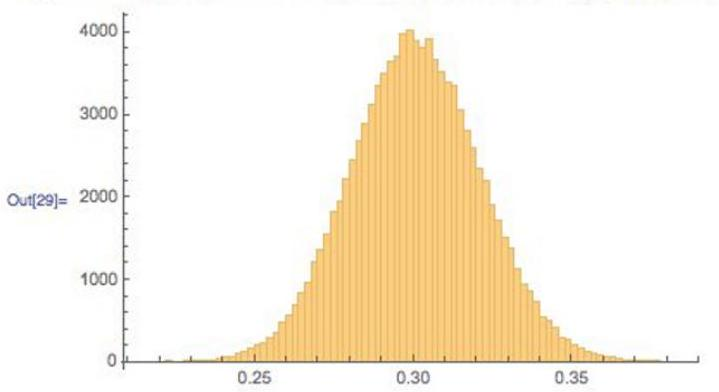
\includegraphics[max width=\textwidth]{2025_03_17_ca60ec0bfd96dcf8e028g-055}
  \caption{Sample variance on hitters with a real 30\% success rate results in a wide range of observed performance even over 500 trials per season.}
\end{figure}

चित्र 2.5 एक सरल सिम्यूलेशन के परिणाम दिखाता है, जहाँ प्रत्येक एट-बैट के परिणाम को तय करने के लिए बेतरतीब संख्याओं का उपयोग किया गया था, 500 एट-बैट प्रति सीज़न। हमारा कृत्रिम खिलाड़ी एक वास्तविक .300 हिटर है, क्योंकि हमने इसे हिट की रिपोर्ट करने के लिए प्रोग्राम किया है प्रोबेबिलिटी$300 / 1000$(0.3) के साथ। परिणाम बताते हैं कि एक वास्तविक .300 हिटर के पास 10\% संभावना होती है कि वह .275 या उससे नीचे हिट करे, सिर्फ संयोग से। ऐसे सीज़न को आमतौर पर चोटों या शायद उम्र के एथलेटिक प्रदर्शन पर अनिवार्य प्रभावों द्वारा समझाया जाता है। लेकिन यह सिर्फ प्राकृतिक विचलन भी हो सकता है। समझदार टीमें एक खराब सीज़न के बाद एक अच्छे हिटर को प्राप्त करने की कोशिश करती हैं, जब कीमत सस्ती होती है, इस विचलन का फायदा उठाने की कोशिश करते हुए।

हमारा .300 हिटर भी .325 से ऊपर बल्लेबाजी करने का 10% संभावना रखता है, लेकिन आप...

%---- Page End Break Here ---- Page : 38

यह सुनिश्चित किया जा सकता है कि वे ऐसे सफल सीजन को अपनी सुधरी हुई फिटनेस या ट्रेनिंग विधियों का श्रेय देंगे बजाय इसके कि यह कहने के कि वे बस किस्मत वाले थे। अच्छा या बुरा सीजन, या भाग्यशाली/दुर्भाग्यशाली: संकेत को शोर से अलग करना कठिन होता है।

\begin{itemize}
  \item \textit{मॉडल प्रदर्शन}: डेटा वैज्ञानिकों के रूप में, हम प्रत्येक भविष्यवाणी चुनौति के लिए आमतौर पर कई मॉडलों का विकास और मूल्यांकन करेंगे। ये मॉडल बहुत सरल से लेकर जटिल तक हो सकते हैं, और उनके प्रशिक्षण स्थितियों या पैरामीटरों में भिन्नता हो सकती है।
\end{itemize}

आमतौर पर, जिस मॉडल ने प्रशिक्षण कोरपस पर सबसे अच्छी सटीकता दिखाई होती है, उसे गर्व के साथ दुनिया के सामने सही मॉडल के रूप में प्रस्तुत किया जाता है। लेकिन मॉडलों के प्रदर्शन में छोटे अंतर को आमतौर पर साधारण परिवर्तनशीलता द्वारा समझाया जा सकता है न कि बुद्धिमत्ता द्वारा: कौन से ⸨प्रशिक्षण/मूल्यांकन⸩ युग्म चुने गए, कितनी अच्छी तरह पैरामीटर्स ऑप्टिमाइज़ किए गए, आदि।\\
मशीन लर्निंग मॉडल्स के प्रशिक्षण के समय इस बात को याद रखना चाहिए। वास्तव में, जब इनका प्रदर्शन बहुत अधिक अलग नहीं होता, तब मैं सबसे सरल मॉडल के पक्ष में तर्क देने की अधिक संभावना रखता हूँ बजाय सबसे उच्च स्कोर वाले मॉडल के। सौ लोगों को सिक्के के उछाल के माध्यम से 'हेड्स' और 'टेल्स' की भविष्यवाणी करने के लिए कहें, तो उनमें से एक निश्चित रूप से सबसे सही उत्तर देगा। लेकिन इसका कोई कारण नहीं है यह मानने का कि इस व्यक्ति के पास हममें से बाकी से बेहतर भविष्यवाणी करने की शक्ति है।

\subsection{वितरणों का विशेषण}
वितरणों में आवश्यक रूप से ज्यादातर संभाव्यता द्रव्यमान ठीक औसत पर नहीं होता। विचार करें कि आपका धन कैसा दिखेगा जब आप\$100 मिलियन उधार लें, और फिर उसे एक समान पैसे वाले सिक्के की बाज़ी पर दांव लगाएं। अगर सिर आए, तो आप अब\$100 मिलियन के साफ हैं, और अगर पूंछ आए, तो आप\$100 मिलियन के ऋण में हैं। आपकी अपेक्षित धनराशि शून्य है, लेकिन यह औसत आपकी धन वितरण के आकार के बारे में ज्यादा नहीं बताता।\index{crowdsourcing}

हालाँकि, औसत और मानक विचलन मिलकर किसी भी\textit{वितरण}का वर्णन करने का एक अच्छा काम करते हैं। औसत से दूर स्थित थोड़ा सा द्रव्यमान भी मानक विचलन में काफी वृद्धि करेगा, इसलिए एक छोटा मान $\sigmaइंगित करता है कि द्रव्यमान का अधिकांश भाग औसत के पास होना चाहिए।

यथार्थ रूप से, चाहे आपका डेटा किसी भी प्रकार से वितरित हो, कम से कम$(1 - (1 / k^2))$भाग मात्रा माध्यिका के$k\pmमानक विचलनों के भीतर अवश्य आनी चाहिए। इसका अर्थ है कि कम से कम$75\%$सभी डेटा माध्यिका के$2$\sigmaके भीतर आनी चाहिए, और लगभग$89\%$के भीतर$3$\sigmaकिसी भी वितरण के लिए।

हम देखेंगे कि जब हमें ज्ञात है कि वितरण अच्छी तरह से व्यवस्थित है, जैसे गॉसियन या सामान्य वितरण, तो और भी सख्त सीमाएँ लागू होती हैं। लेकिन इसी कारण यह एक उत्तम प्रथा है कि जब भी आप औसत के बारे में बात करें तो दोनों$\mu$और$\sigma$की सूचना दी जाए। संयुक्त राज्य अमेरिका में वयस्क महिलाओं की औसत ऊँचाई $63.7\pm2.7$इंच है, जिसका अर्थ है$\mu=63.7$और$\sigma=2.7$। ऑरलैंडो, फ्लोरिडा में औसत तापमान 60.3 डिग्री फारेनहाइट है। हालांकि, डिज्नी वर्ल्ड में 100 डिग्री के दिनों की संख्या महिलाओं की 100 इंच (8.33 फीट) की संख्या की तुलना में अधिक रही है जो इस आनंद को लेने आई हैं।

\textit{घर का सबक}: अपनी वितरण को वर्णित करने के लिए औसत और मानक विचलन दोनों को रिपोर्ट करें, इसे इस प्रकार लिखा जाता है$\mu\pm\sigma$.\index{Darwin, Charles}\index{Galton, Francis}

\section{सहसंबंध विश्लेषण}
\index{social media!analysis}\index{coordination!analysis}मान लीजिए हमें दो चर$x$और$y$दिए गए हैं, जिन्हें$n$बिंदुओं के नमूने के रूप में दर्शाया गया है, रूप$(x_{i}, y_{i})$, जहाँ$1\leqi\leqn$। हम कहते हैं कि$x$और$y$\textit{सहसंबद्ध}हैं जब$x$का मूल्य$y$के मूल्य पर कुछ भविष्यवाणी शक्ति रखता है।\index{anchoring}\index{Surowiecki, James}

\textit{सहसंबंध गुणांक} $r(X, Y)$ एक सांख्यिकी है जो मापता है कि किस हद तक $Y$, $X$ का एक फलन है, और इसके विपरीत। सहसंबंध गुणांक का मान -1 से 1 तक होता है, जहाँ 1 का अर्थ पूरी तरह से संबंधित और 0 का मतलब कोई संबंध नहीं, या स्वतंत्र चरों होता है। नकारात्मक सहसंबंध इंगित करते हैं कि चर \textit{विरुद्ध-संबंधित} हैं, जिसका मतलब है कि जब $X$ बढ़ता है, तो $Y$ घटता है।

संपूर्ण रूप से प्रतिलोम सहसंबद्ध चर -1 का सहसंबंध रखते हैं। ध्यान दें कि नकारात्मक सहसंबंध भविष्यवाणी के उद्देश्यों के लिए उतने ही अच्छे होते हैं जितने सकारात्मक। यह कि आपके बेरोजगार होने की संभावना कम हो जाती है जब आपकी शिक्षा अधिक होती है, एक नकारात्मक सहसंबंध का उदाहरण है, इसलिए शिक्षा का स्तर वास्तव में नौकरी की स्थिति का पूर्वानुमान लगाने में मदद कर सकता है। 0 के आसपास के सहसंबंध पूर्वानुमान के लिए बेकार होते हैं।

देखी गई सहसंबंध उन कई पूर्वानुमान मॉडल्स को आगे बढ़ाते हैं जिन्हें हम डेटा विज्ञान में बनाते हैं। सहसंबंधों की प्रातिनिधिक ताकतों में शामिल हैं:

\begin{itemize}
  \item क्या लंबे लोग अधिक दुबले रहने की संभावना रखते हैं? ऊँचाई और बीएमआई के बीच देखी गई सहसंबंध $r=-0.711$ है, इसलिए ऊँचाई वास्तव में बॉडी मास इंडेक्स (बीएमआई) के साथ नकारात्मक रूप से सहसंबंधित है।\footnote{\url{https://onlinecourses.science.psu.edu/stat500/node/60}}
  \item क्या मानकीकृत परीक्षण कॉलेज में छात्रों के प्रदर्शन की भविष्यवाणी करते हैं? SAT स्कोर और फ्रेशमेन GPA के बीच देखी गई सहसंबंध $r=0.47$ है, इसलिए हाँ, इसमें कुछ भविष्यवाणी शक्ति है। लेकिन सामाजिक आर्थिक स्थिति SAT स्कोर के साथ उतनी ही मजबूती से सहसंबंधित है $(r=0.42)$।\footnote{\url{https://research.collegeboard.org/sites/default/files/publications/2012/9/researchreport-2009-1-socioeconomic-status-sat-freshman-gpa-analysis-data.pdf}}
   \item क्या वित्तीय स्थिति स्वास्थ्य को प्रभावित करती है? घरेलू आय और कोरोनरी धमनी रोग की प्रचलता के बीच देखी गई सहसंबंध $r=-0.717$ है, इसलिए एक मजबूत नकारात्मक सहसंबंध है। इसलिए हाँ, जितने आप समृद्ध होंगे, आपके दिल के दौरे का जोखिम उतना ही कम होगा।\footnote{\url{http://www.ncbi.nlm.nih.gov/pmc/articles/PMC3457990/}}
  \item क्या धूम्रपान स्वास्थ्य को प्रभावित करता है? धूम्रपान करने की प्रवृत्ति और उनकी मृत्यु दर के बीच देखी गई सहसंबंध $r=0.716$ है, इसलिए परमात्मा के लिए, धूम्रपान ना करें।\footnote{\url{http://lib.stat.cmu.edu/DASL/Stories/SmokingandCancer.html}}
  \item क्या हिंसात्मक वीडियो गेम आक्रामक व्यवहार में वृद्धि करते हैं? खेल और हिंसा के बीच देखी गई सहसंबंध $r=0.19$ है, इसलिए एक कमजोर लेकिन महत्वपूर्ण सहसंबंध है।\footnote{\url{http://webspace.pugetsound.edu/facultypages/cjones/chidev/Paper/Articles/Anderson-Aggression.pdf}}\index{aggregation mechanisms}\index{Amazon Turk}\index{Amazon Turk!Turkers}\index{Arrow’s impossibility theorem}\index{Condorcet jury theorem}\index{CrowdFlower}\index{crowdsourcing services}\index{weighted average}
\end{itemize}

इस खंड में सहसंबंध के मुख्य मापों का परिचय दिया जाएगा। आगे बढ़ते हुए, हम अध्ययन करेंगे कि कैसे किसी भी देखे गए सहसंबंध की ताकत और प्रभाव को उपयुक्त रूप से निर्धारित किया जाए, ताकि हमें यह समझने में मदद मिल सके कि चर के बीच संबंध वास्तविक कब हैं।

\subsection{संबंध गुणांक: पीयरसन और स्पीयरमैन रैंक}
वास्तव में, संबंध को मापने के लिए दो मुख्य सांख्यिकी का उपयोग किया जाता है। सौभाग्य से, दोनों एक ही$-1$से$1$पैमाने पर काम करते हैं, हालांकि वे अलग-अलग चीजों को मापते हैं। ये अलग-अलग सांख्यिकी अलग-अलग परिस्थितियों में उपयुक्त होते हैं, इसलिए आपको इनमें से दोनों के बारे में जागरूक होना चाहिए।

\subsection{पियरसन सहसंबंध गुणांक}
इन दो सांख्यिकी में अधिक प्रमुख पियरसन सहसंबंध है, जिसे परिभाषित किया गया है

\[ r = \frac{\sum_{i=1}^{n}(X_{i}-\bar{X})(Y_{i}-\bar{Y})}{\sqrt{\sum_{i=1}^{n}(X_{i}-\bar{X})^{2}} \sqrt{\sum_{i=1}^{n}(Y_{i}-\bar{Y})^{2}}} = \frac{\operatorname{Cov}(X, Y)}{\sigma(X) \sigma(Y)} \]

चलो इस समीकरण का विश्लेषण करते हैं। मान लीजिए कि$X$और$Y$मजबूत रूप से संबंधिक हैं। तब हम उम्मीद करेंगे कि जब$x_{i}$उसके औसत$\bar{X}$से अधिक है, तब$y_{i}$को भी उसके औसत$\bar{Y}$से अधिक होना चाहिए। जब$x_{i}$उसके औसत से कम होता है,$y_{i}$को भी वैसा ही होना चाहिए। अब गिनीक के अंश पर नज़र डालें। हर एक पद का चिह्न सकारात्मक होता है जब दोनों मान$(1\times1)$से ऊपर या$(-1\times-1)$से नीचे उनके संबंधित औसत से होते हैं। हर एक पद का चिह्न नकारात्मक$((-1\times1)$या$(1\times-1))$तब होता है जब वे विपरीत दिशाओं में चलते हैं, जिससे नकारात्मक संबंध होता है। अगर$X$और$Y$असंबंधित होते, तो सकारात्मक और नकारात्मक पद समान आवृत्ति से आते, एक-दूसरे को संतुलित करते और मूल्य को शून्य की ओर ले जाते।

हनुमानक के ऑपरेशन के चिन्ह का निर्धारण संबंध की दिशा को इतना उपयोगी बनाता है कि हम इसे एक नाम देते हैं, सह-संबंध, गणना की गई:

\[\operatorname{सहसंबंध}(X, Y) =\sum_{i=1}^{n}(X_{i}-\bar{X})(Y_{i}-\bar{Y})\]\index{machine learning!classifiers}

कॊवेरिअंस को याद रखें: हम इसे फिर से अनुभाग 8.2.3 में देखेंगे।\\
पियरसन फॉर्मूला के हर का उन दो चर में परिवर्तनशीलता को प्रदर्शित करता है, जैसा कि उनकी मानक विचलन द्वारा मापा जाता है। X और Y के बीच का कॊवेरिअंस संभावित रूप से इन चरों के परिवर्तनशीलता के साथ बढ़ता है, और यह हर वह जादुई मात्रा है जिससे विभाजित करने पर सहसंबंध$-1$से$1$तक के पैमाने में आ जाता है।\index{A/B testing}\index{CrowdFlower}\index{Emoji Dick}\index{Moby Dick}\index{Sheep Market}

%---- Page End Break Here ---- Page : 41





\begin{figure}[h]
    \centering
    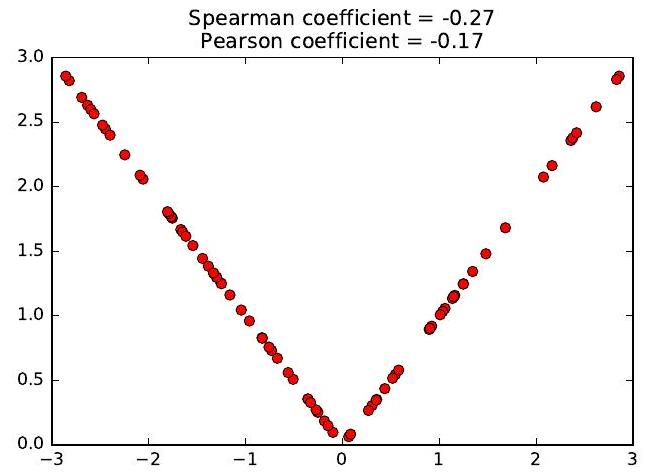
\includegraphics[max width=\textwidth]{2025_03_17_ca60ec0bfd96dcf8e028g-059}
    \caption{The function $y=|x|$ does not have a linear model, but seems like it should be easily fitted despite weak correlations.}
    \label{fig:abs-function}
\end{figure}

पीयरसन सहसंबंध गुणांक यह परिभाषित करता है कि एक रैखिक पूर्वानुमानकर्ता जिसका रूप $y=mx+b$ होता है, वह अवलोकित डेटा के साथ कितनी मात्रा में फिट हो सकता है। यह सामान्यतः चर के बीच समानता को मापने का अच्छा काम करता है, लेकिन ऐसे विकृत उदाहरण बनाना संभव है जहां $X$ और $Y$ के बीच सहसंबंध गुणांक शून्य हो, फिर भी $Y$ पूरी तरह से $X$ पर निर्भर हो (और इसलिए @X@ से पूर्णतः भविष्यवाणी योग्य हो)।

ध्यान दें कि रूप$(x,|x|)$के बिंदु हैं, जहाँ पर$x$को अंतराल$[-1,1]$से समान रूप से (या सममित रूप से) नमूना लिया जाता है जैसा \ref{चित्र:abs-function}में दिखाया गया है। सहसंबंध शून्य होगा क्योंकि प्रत्येक बिंदु$(x, x)$के लिए एक संतुलन बिंदु$(-x, x)$उपलब्ध होगा, फिर भी$y=|x|$एक पूर्ण भविष्यवाणी करने वाला है। पीअर्सन सहसंबंध मापता है कि सर्वश्रेष्ठ रैखिक पूर्वसूचक कितनी अच्छी तरह कार्य कर सकते हैं, लेकिन इसे विचित्र गणनाओं जैसे पूर्ण मान के बारे में कुछ नहीं कहता।

स्पीयरमैन रैंक सहसंबंध गुणांक मूलतः इनपुट बिंदुओं की युगलियों को गिनता है जो क्रम से बाहर होते हैं। मान लीजिए कि हमारे डेटा सेट में बिंदु$\left(x_{1}, y_{1}\right)$और$\left(x_{2}, y_{2}\right)$शामिल हैं जहाँ$x_{1}< x_{2}$और$y_{1}< y_{2}$। यह एक मतदान है कि मान सकारात्मक रूप से सहसंबंधित हैं, जबकि यदि$y_{2}< y_{1}$तो मतदान नकारात्मक सहसंबंध के लिए होगा।

सभी बिंदुओं की जोड़ीओं पर योग करके और सही तरीके से सामान्यीकृत करके हमें स्पीयरमैन रैंक सहसंबंध प्राप्त होता है। मान लीजिए कि$\operatorname{rank}\left(x_{i}\right)$x_{i}$का सभी$x_{i}$में क्रमबद्ध क्रम में रैंक स्थिति है, इसलिए सबसे छोटे मान की रैंक 1 है और सबसे बड़े मान की$n$। फिर

\[
\rho=1-\frac{6 \sum d_{i}^{2}}{n\left(n^{2}-1\right)}
\]

where$d_{i}=\operatorname{रैंक}\left(x_{i}\right)-\operatorname{रैंक}\left(y_{i}\right)$.

\begin{figure}[h]
    \centering
    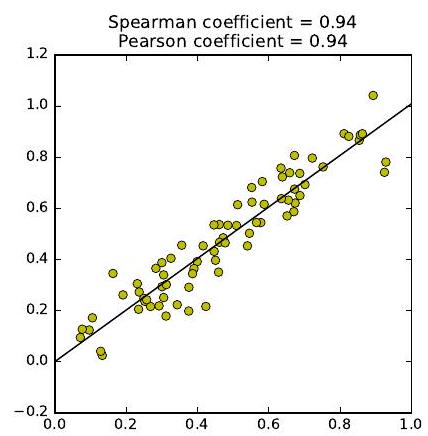
\includegraphics[max width=\textwidth]{2025_03_17_ca60ec0bfd96dcf8e028g-060}
    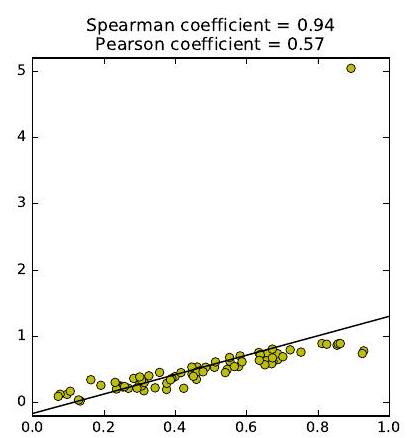
\includegraphics[max width=\textwidth]{2025_03_17_ca60ec0bfd96dcf8e028g-060(1)}
    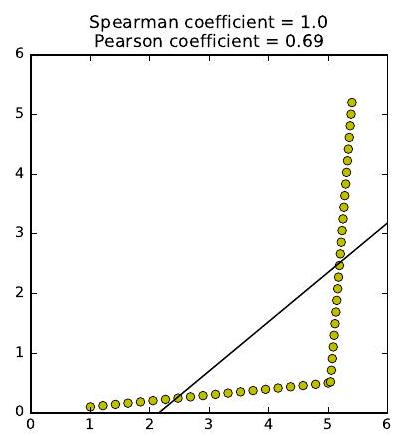
\includegraphics[max width=\textwidth]{2025_03_17_ca60ec0bfd96dcf8e028g-060(2)}
    \caption{A monotonic but not linear point set has a Spearman coefficient $r=1$ even though it has no good linear fit (left). Highly-correlated sequences are recognized by both coefficients (center), but the Pearson coefficient is much more sensitive to outliers (right).}\index{games with a purpose}\index{gamification}\index{institutional review board}
    \label{fig:spearman-pearson}
\end{figure}

गैर-रेखीय लेकिन मोनोटोनिक फ़ंक्शनों को उच्च अंक देने के अलावा, स्पीयरमैन सहसंबंध पीयर्सन की तुलना में अत्यधिक बाहरी तत्वों के प्रति कम संवेदनशील होता है। मान लें कि$p=(x_{1}, y_{\max})$वह डेटा बिंदु है जिसके पास दिए गए डेटा सेट में$y$का सबसे बड़ा मान होता है। मान लीजिए कि हम$p$को$p'=(x_{1},\infty)$से बदल देते हैं। पीयर्सन सहसंबंध विचलित हो जाएगा, क्योंकि सबसे अच्छा फिट अब लंबवत रेखा$x=x_{1}$बन जाता है। लेकिन स्पीयरमैन सहसंबंध अपरिवर्तित रहेगा, क्योंकि सभी बिंदु पहले$p$के नीचे थे, जैसे कि वे अब$p'$के नीचे हैं।

\subsection{सहसंबंध की शक्ति और महत्व}

कोरिलेशन कोएफिशिएंट $r$ उस सीमा को दर्शाता है जिस तक $x$ को किसी दिए गए बिंदुओं के नमूने $S$ में $y$ की भविष्यवाणी करने के लिए उपयोग किया जा सकता है। जैसे-जैसे $|r|\rightarrow 1 की ओर बढ़ता है, ये भविष्यवाणियाँ बेहतर और बेहतर होती जाती हैं।

लेकिन असली सवाल ये है कि वास्तविक दुनिया में, नमूने के बाहर, यह संबंध कैसे बना रहेगा। मजबूत सम्बन्धों के पास बड़ा$|r|$ होता है, लेकिन इसमें पर्याप्त बिंदुओं के नमूने शामिल होते हैं ताकि यह महत्वपूर्ण हो सके। एक मज़ाकिया कहावत है कि अगर आप अपने डेटा को सीधी रेखा से फिट करना चाहते हैं, तो इसे केवल दो बिंदुओं पर नमूना लेना सबसे अच्छा होता है। आपका सम्बन्ध जितने अधिक बिंदुओं पर आधारित होता है, उतना अधिक प्रभावशाली बन जाता है।

व्याख्या में सहसंबंधों की सांख्यिकीय सीमाएँ चित्र\ref{fig:correlation-limits}में ताकत और आकार के आधार पर प्रस्तुत की जाती हैं।

\begin{itemize}
  \item \textbf{Strength of correlation: $R^{2}$ :} The square of the sample correlation coefficient $r^{2}$ estimates the fraction of the variance in $Y$ explained by $X$ in a simple linear regression. The correlation between height and weight is approximately 0.8, meaning it explains about two-thirds of the variance.
  
  \begin{figure}[h]
      \centering
      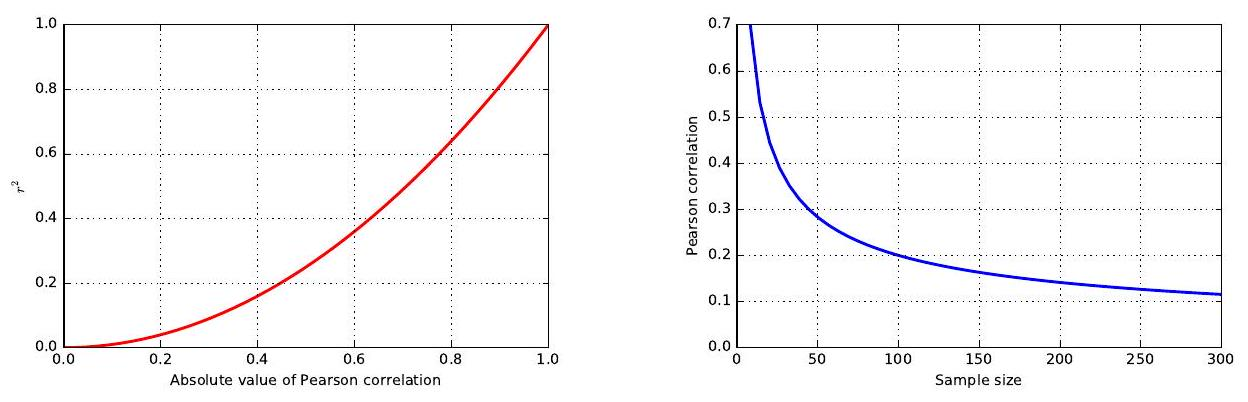
\includegraphics[max width=\textwidth]{2025_03_17_ca60ec0bfd96dcf8e028g-061(1)}
      \caption{Limits in interpreting significance. The $r^{2}$ value shows that weak correlations explain only a small fraction of the variance (left). The level of correlation necessary to be statistically significant decreases rapidly with sample size $n$ (right).}
      \label{fig:correlation-limits}
  \end{figure}
  
  Figure \ref{fig:correlation-limits} (left) shows how rapidly $r^{2}$ decreases with $r$. There is a profound limit to how excited we should get about establishing a weak correlation. A correlation of 0.5 possesses only 25\% of the maximum predictive power, and a correlation of $r=0.1$ only 1\%. Thus, the predictive value of correlations decreases rapidly with $r$.
\end{itemize}

हम "वेरिएंस को समझाना" क्या मतलब है? मान लीजिए $f(x)=mx+c$ $x$ से $y$ के लिए भविष्यवाणी मूल्य है, जहाँ $m$ और $c$ सबसे अच्छे संभव फिट के लिए पैरामीटर हैं। अवशिष्ट मूल्य $r_{i}=y_{i}-f\left(x_{i}\right)$ का औसत शून्य होगा, जैसा कि चित्र \ref{fig:residuals} में दिखाया गया है। आगे, यदि $f(x)$ का अच्छा रैखिक फिट है, तो पूर्ण डेटा सेट $V(Y)$ का वेरिएंस $V(r)$ से बहुत बड़ा होना चाहिए। यदि $x$ और $y$ पूरी तरह से सहसंबद्ध हैं, तो कोई अवशिष्ट त्रुटि नहीं होनी चाहिए, और $V(r)=0$ होगा। यदि $x$ और $y$ पूरी तरह से असंबद्ध हैं, तो फिट में कुछ भी योगदान नहीं देना चाहिए, और $V(y)\approx $V(r)$। सामान्यतः, $1-r^{2}=V(r) / V(y)@।\index{Babbage, Charles}\index{exercises}

\begin{figure}[h]
    \centering
    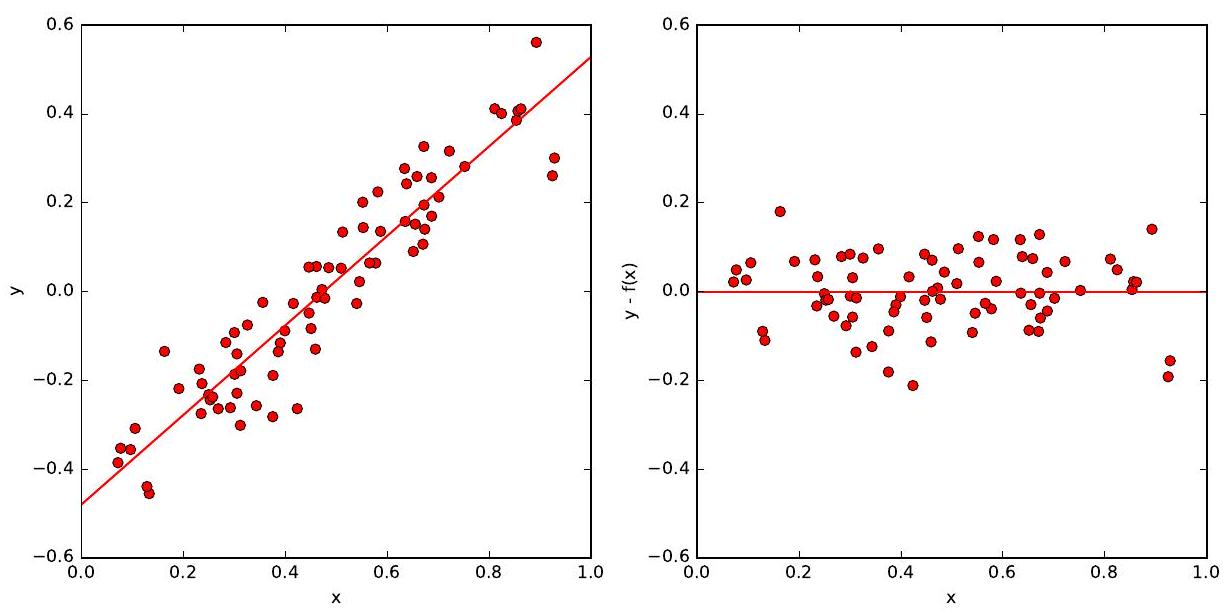
\includegraphics[max width=\textwidth]{2025_03_17_ca60ec0bfd96dcf8e028g-061}
    \caption{Plotting $r_{i}=y_{i}-f\left(x_{i}\right)$ shows that the residual values have lower variance and mean zero. The original data points are on the left, with the corresponding residuals on the right.}
    \label{fig:residuals}
\end{figure}

चित्र\ref{fig:residuals} पर विचार करें, जिसमें एक बाईं ओर बिंदुओं का सेट दिखाया गया है, जो एक अच्छा रैखिक फिट प्रदान करती है, सहसंबंध$r=0.94$ के साथ। संबंधित अवशेष$r_{i}=y_{i}-f\left(x_{i}\right)$ दाईं ओर चित्रित किए गए हैं। बाईं ओर$V(y)=0.056$ का$y$ मान का विचलन, दाईं ओर विचलन$V(r)=0.0065$ की तुलना में काफी अधिक है। वास्तव में,

\[
1-r^{2}=0.116 \longleftrightarrow V(r) / V(y)=0.116
\]

\begin{itemize}
  \item \textbf{सांख्यिकीय महत्व:} एक संबंध का सांख्यिकीय महत्व उसके नमूने के आकार $n$ के साथ-साथ $r$ पर निर्भर करता है। परंपरागत रूप से, हम कहते हैं कि एक संबंध $n$ बिंदुओं का महत्वपूर्ण होता है यदि कोई $\alpha \leq 1 / 20=0.05$ संभावना है कि हम $r$ के रूप में एक मजबूत संबंध को किसी भी यादृच्छिक $n$ बिंदुओं के सेट में देखेंगे।
  
  यह विशेष रूप से मजबूत मानक नहीं है। यहां तक कि छोटे संबंध भी 0.05 स्तर पर महत्वपूर्ण हो जाते हैं जब नमूनों का आकार पर्याप्त बड़ा होता है, जैसा कि चित्र \ref{fig:correlation-limits} (दाएं) में दिखाया गया है। $r=0.1$ का संबंध $\alpha$= 0.05$$ के आसपास @n=300@ पर महत्वपूर्ण हो जाता है, भले ही ऐसा कारक केवल 1\% परिवर्तनशीलता को समझाता है।
\end{itemize}

कमजोर लेकिन महत्वपूर्ण सहसंबंध बड़े डेटा मॉडलों में मूल्यवान हो सकते हैं जिनमें विशेषताओं की बड़ी संख्या शामिल होती है। कोई भी एकल विशेषता/सहसंबंध केवल छोटे प्रभावों को समझा/परेखना कर सकता है, लेकिन एक साथ लिया गया, कमजोर लेकिन स्वतंत्र सहसंबंधों की एक बड़ी संख्या में मजबूत पूर्वानुमान शक्ति हो सकती है। शायद। हम अनुभाग 5.3 में महत्व को फिर से और विस्तार से चर्चा करेंगे।

\subsection{संबंध कारण नहीं दर्शाता है!}
आपने इसे पहले सुना होगा: संबंध कारण नहीं दर्शाता है:

\begin{itemize}
  \item किसी प्रीसिंक्ट में सक्रिय पुलिस की संख्या स्थानीय अपराध दर के साथ मजबूत संबंध रखती है, लेकिन पुलिस अपराध का कारण नहीं बनती। 
  \item लोगों द्वारा ली जाने वाली दवा की मात्रा इस बात की संभावना से संबंधित होती है कि वे बीमार हैं, लेकिन दवा बीमारी का कारण नहीं बनती। 
\end{itemize}

सर्वोत्तम स्थिति में, निहितार्थ केवल एक ही दिशा में काम करता है। लेकिन कई देखे गए सहसंबंध पूरी तरह से मिथ्या हैं, जिनमें से किसी भी चर का दूसरे पर कोई वास्तविक प्रभाव नहीं होता है।

फिर भी,\textit{सांख्यिकीय सहसंबंध कारण का संकेत करता है}सोच में एक सामान्य त्रुटि होती है, यहां तक कि उनके बीच भी जो तार्किक विचारधारा समझते हैं। सामान्य रूप से कहा जाए तो, कुछ सांख्यिकीय उपकरण उपलब्ध होते हैं ताकि यह पता चल सके कि$A$वास्तव में$B$का कारण बनता है या नहीं। हम नियंत्रित प्रयोग कर सकते हैं, यदि हम एक चर को नियंत्रित करके दूसरे पर प्रभाव देख सकें। उदाहरण के लिए, यह तथ्य कि हम लोगों को ऐसा आहार दे सकते हैं जो उनका वजन कम कर देता है बिना उनकी लंबाई घटाए, यह विश्वास दिलाने वाला साक्ष्य है कि वजन लंबाई का कारण नहीं है। लेकिन अक्सर इन प्रयोगों को दूसरी तरफ से करना कठिन होता है, जैसे कि, लोगों की लंबाई कम करने का कोई उचित तरीका नहीं है जब तक कि उनके अंगों को नहीं काटा जाए।

\begin{figure}[h]
    \centering
    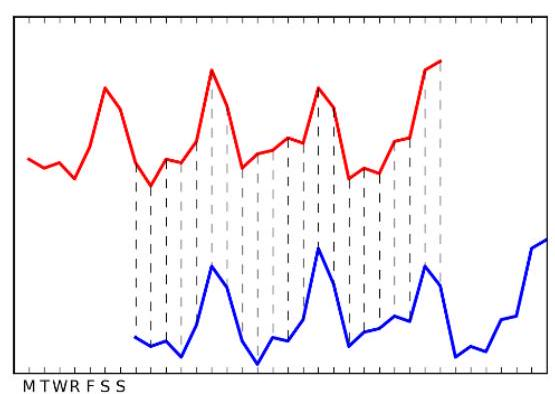
\includegraphics[max width=\textwidth]{2025_03_17_ca60ec0bfd96dcf8e028g-063}
    \caption{Correlation does not imply causation. (Source \href{https://www.xkcd.com/552}{https://www.xkcd.com/552})}
    \label{fig:correlation-causation}
\end{figure}

\begin{figure}[h]
    \centering
    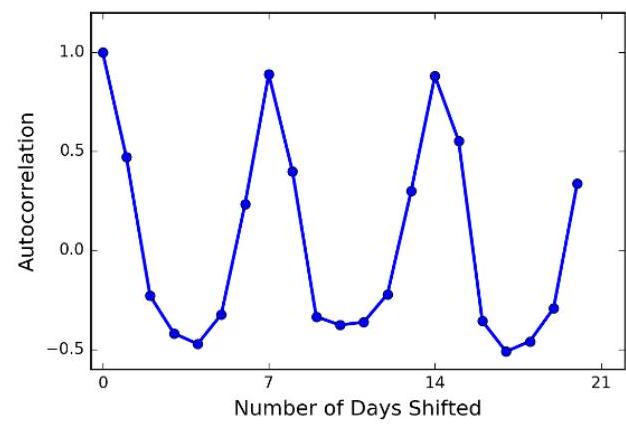
\includegraphics[max width=\textwidth]{2025_03_17_ca60ec0bfd96dcf8e028g-063(1)}
    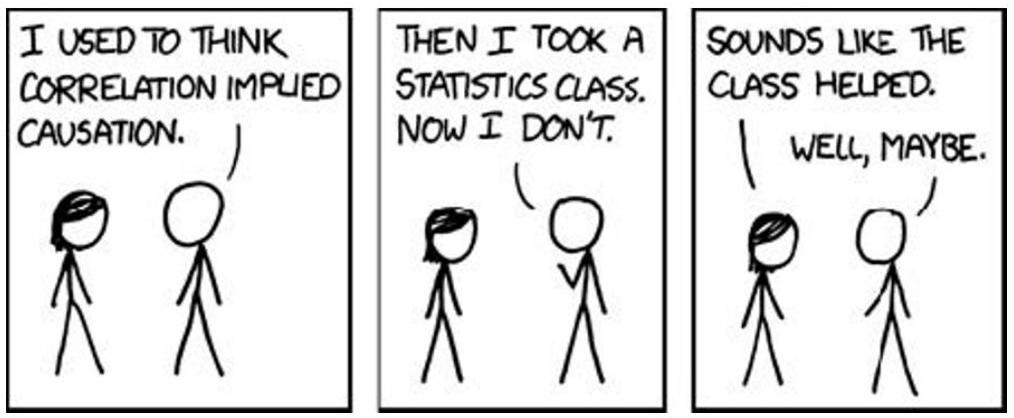
\includegraphics[max width=\textwidth]{2025_03_17_ca60ec0bfd96dcf8e028g-063(2)}
    \caption{Cyclic trends in a time series (left) are revealed through correlating it against shifts of itself (right).}
    \label{fig:cyclic-trends}
\end{figure}

\subsection{स्वतःसंबंधन द्वारा आवृत्तियों का पता लगाना}
कल्पना करें कि एक अंतरिक्ष एलियन को एक खिलौना कंपनी में अमेरिकी बिक्री का विश्लेषण करने के लिए काम पर रखा गया। एक सुंदर सुचारु प्रवृत्ति दिखाने वाले फ़ंक्शन के बजाय, वे प्रत्येक बारहवें महीने, हर साल, एक विशाल उछाल देखकर चकित होंगे। इस एलियन ने क्रिसमस की घटना की खोज कर ली होगी।

मौसमी प्रवृत्तियाँ निश्चित अवधि के चक्र को दर्शाती हैं, जो नियमित पैटर्न में ऊपर और नीचे होती हैं। कई मानवी गतिविधियाँ कार्य सप्ताह से संबंधित सात-दिवसीय चक्र के साथ आगे बढ़ती हैं। एक प्रकार के कीड़े की बड़ी आबादी जिसे \textit{सिकाडा} कहा जाता है, 13-वर्षीय या 17-वर्षीय चक्र में उभरती है, ताकि शिकारी उन्हें न सीख सकें...%---- पृष्ठ समाप्ति विराम यहाँ ---- पृष्ठ : 46

हम किसी क्रम में ऐसे चक्रीय पैटर्न को कैसे पहचान सकते हैं? मान लीजिए हम$S_i$के$S_{i+p}$के साथ मूल्यों का संबंध देखते हैं, सभी$1$i$n-p\leqके लिए। यदि कुछ विशेष अवधि लंबाई\leqp$के लिए मूल्य संपर्क में होते हैं, तो अन्य संभावित अंतराल मूल्यों की तुलना में इसके साथ संबंध असाधारण रूप से उच्च होगा। किसी क्रम की तुलना खुद से करना\textit{आटोकोरिलेशन}कहलाता है, और सभी$1$k$n-1\leqके लिए संबंधों की श्रृंखला को\textit{आटोकोरिलेशन फ़ंक्शन}कहा जाता है। चित्र 2.11 दैनिक बिक्री का समय श्रृंखला प्रस्तुत करता है, और इस डेटा के लिए संबंधित आटोकोरिलेशन फ़ंक्शन। सात दिनों के स्थानांतरण पर और सात के आवर्तक पर सर्वोच्च बिंदु यह स्थापित करता है कि बिक्री में साप्ताहिक आवधिकता है: सप्ताहांत में अधिक सामग्री बिकती है।

ऑटोकॉरिलेशन भविष्य की घटनाओं की भविष्यवाणी में एक महत्वपूर्ण संकल्पना है, क्योंकि इसका अर्थ है कि हम पहले के प्रेक्षणों का उपयोग मॉडल में विशेषताओं के रूप में कर सकते हैं। यह अनुमान कि कल का मौसम आज के मौसम के समान होगा, ऑटोकॉरिलेशन पर आधारित है, जिसमें$p=1$दिन का विलंब है। निश्चित रूप से, हम उम्मीद करेंगे कि ऐसा मॉडल छह महीने पहले के मौसम डेटा पर बनाए गए अनुमानों की तुलना में अधिक सटीक होगा (विलंब$p=180$दिन)।

सामान्य तौर पर, कई मात्राओं के लिए स्वयंसंबंधित फलन बहुत छोटे विलंबों के लिए सबसे अधिक होता है। यही कारण है कि दीर्घकालीन भविष्यवाणियाँ अल्पकालिक पूर्वानुमानों की तुलना में कम सटीक होती हैं: स्वयंसंबंधित प्रभाव आम तौर पर बहुत कमजोर होते हैं। लेकिन आवधिक चक्र कभी-कभी बहुत लंबे समय तक खिंच सकते हैं। वास्तव में, $p=365$ दिनों के विलंब पर आधारित मौसम पूर्वानुमान $p=180$ की तुलना में कहीं बेहतर होगा, क्योंकि मौसमी प्रभाव होते हैं।

पूरी ऑटोकॉरिलेशन फंक्शन की गणना करने के लिए समय श्रृंखला के बिन्दुओं पर$n-1$विभिन्न संबंधों की गणना करनी पड़ती है, जो बड़े$n$के लिए महंगा हो सकता है। सौभाग्य से, एक कुशल एल्गोरिदम \textit{फास्ट फूरियर ट्रांसफॉर्म}(FFT) पर आधारित है, जो बहुत लंबी अनुक्रमों के लिए भी ऑटोकॉरिलेशन फंक्शन का निर्माण करना संभव बनाता है।

\section{लघुगणक}
\textit{लघुगणक} विपरीत घातांक फलन है$y = b^{x}$, एक समीकरण जिसे इस प्रकार लिखा जा सकता है$x =\log_{b}y$। यह परिभाषा उस बात के समान है जो कहती है कि

$$
b^{\log_{ब} व}= व.
$$

घातांक फ़ंक्शन बहुत तेज़ गति से बढ़ते हैं: पर विचार करें$b =\{2^1, 2^2, 2^3, 2^4,\ldots\}$। इसके विपरीत, लोगारिथम बहुत धीमी गति से बढ़ते हैं: ये पिछले श्रृंखला के केवल घातांक होते हैं$\{1, 2, 3, 4,\ldots\}$। इन्हें किसी भी प्रक्रिया के साथ जोड़ा जाता है जहाँ हम$b$ के कुछ मान से बार-बार गुणा कर रहे होते हैं, या$b$ से बार-बार भाग दे रहे होते हैं। बस परिभाषा याद रखें:

$$
y =\log_{ब}x\longleftrightarrowb^{व}= x
$$

लघुगणक बहुत उपयोगी चीज़ें हैं, और डेटा विश्लेषण में अक्सर उत्पन्न होती हैं। यहाँ मैं डेटा साइंस में लघुगणकों के तीन महत्वपूर्ण भूमिकाओं का विवरण देता हूँ। आश्चर्यजनक रूप से, इनमें से केवल एक ही \textit{दी एल्गोरिदम डिज़ाइन मैनुअल}[Ski08] में प्रस्तुत सात लघुगणकीय अनुप्रयोगों से संबंधित है। वास्तव में लघुगणक बहुत उपयोगी चीज़ें हैं।\index{American basketball players}\index{football!American players}

\subsection{लघुगणक और गुणन संभावनाएँ}
\index{multiplying probabilities}लघुगणक सबसे पहले गणना में सहायक के रूप में आविष्कृत किए गए थे, गुणन की समस्या को जोड़ की समस्या में बदलकर। विशेष रूप से, उत्पाद की गणना करने के लिए$p = x\cdoty$, हम लघुगणकों के जोड़$s =\log_{b}x +\log_{b}y$की गणना कर सकते हैं और फिर लघुगणक के विपरीत (अर्थात $b$ को$s$वी घात में बढ़ाना) लेकर$p$ प्राप्त कर सकते हैं, क्योंकि:\index{scatter plots}

$$
p = x\cdoty = b^{\left(\log_{b} x + \log_{b} y\right)}.
$$

यह वही तरकीब है जो यांत्रिक स्लाइड रूल्स में शक्ति प्रदान करती थी, जिनका उपयोग तकनीकी प्रेमियों द्वारा जेब कैलकुलेटर के पहले के दिनों में किया जाता था।

हालाँकि, यह विचार आज भी महत्वपूर्ण बना हुआ है, विशेष रूप से जब संभावनाओं की लंबी श्रृंखलाओं को गुणा किया जाता है। संभावनाएँ छोटे संख्याएँ होती हैं। इस प्रकार, संभावनाओं की लंबी श्रृंखलाओं को गुणा करने पर बहुत छोटी संख्याएँ उत्पन्न होती हैं जो बहुत दुर्लभ घटनाओं के होने की संभावनाओं को नियंत्रित करती हैं। वास्तविक कंप्यूटरों पर फ्लोटिंग पॉइंट गुणा के साथ गंभीर संख्या स्थिरता समस्याएं होती हैं। संख्यात्मक त्रुटियाँ अंदर आ जाएंगी, और अंततः काफी छोटी संख्याओं के सही मान को दबा देंगी।

संभावनाओं के लॉगरिदम का योग करना उन्हें गुणा करने की तुलना में गणितीय रूप से अधिक स्थिर होता है, लेकिन यह एक समान परिणाम देता है क्योंकि:

$$
\prod_{i=१}^{n}p_{i}= b^{P},\text{ जहाँ }P =\sum_{i=१}^{n}\log_{b}(p_{i})
$$

हम अपने योग को वास्तविक संभावना के लिए घातांक में बदल सकते हैं, लेकिन आमतौर पर यह आवश्यक नहीं होता है। जब हमें केवल दो संभावनाओं की तुलना करनी होती है ताकि यह तय किया जा सके कि कौन सी बड़ी है, तो हम निश्चिंत होकर लॉग की दुनिया में रह सकते हैं, क्योंकि बड़े लघुगणक बड़ी संभावनाओं के अनुरूप होते हैं।

एक बात पर ध्यान दें। याद रखें कि$\log_{2}\left(\frac{1}{2}\right) = -1$. संभावनाओं के लघुगणक सभी ऋणात्मक संख्याएँ होती हैं सिवाय$\log(1) = 0$. यही कारण है कि संभावनाओं के लघुगणक के साथ समीकरणों में अक्सर अजीब जगहों पर ऋणात्मक चिह्न होते हैं। इन पर ध्यान दें।

\subsection{लघुगणक और अनुपात}
\index{ratio}\textit{अनुपात}मात्राएँ $a / b$ के रूप में होती हैं। वे अक्सर डेटा सेटों में या तो प्राथमिक विशेषताओं के रूप में या फीचर जोड़ी से प्राप्त मानों के रूप में दिखाई देती हैं। अनुपात स्वाभाविक रूप से परिस्थितियों के लिए डेटा को सामान्य बनाने में होते हैं (जैसे कुछ उपचार के बाद का वजन बनाम प्रारंभिक वजन) या समय (जैसे आज का मूल्य बनाम कल का मूल्य)।

लेकिन अनुपात बढ़ने और घटने पर अलग-अलग तरीके से व्यवहार करते हैं। ⸨अनुपात$200 / 100$⸩ आधार स्तर से ⸨$200\%$⸩ अधिक है, लेकिन ⸨$100 / 200$⸩ केवल ⸨$50\%$⸩ कम है, बावजूद इसके कि यह एक समान परिमाण परिवर्तन है। इस प्रकार, अनुपात का औसत निकालना एक सांख्यिकीय पाप है। क्या आप सच में चाहते हैं कि एक द्विगुणन के बाद एक अनुसंधान का औसत वृद्धि के रूप में लिया जाए, न कि एक तटस्थ परिवर्तन के रूप में?

%---- Page End Break Here ---- Page : 48

% Mismatched: \chaptername{Logarithms}

\begin{figure}[h]
    \centering
    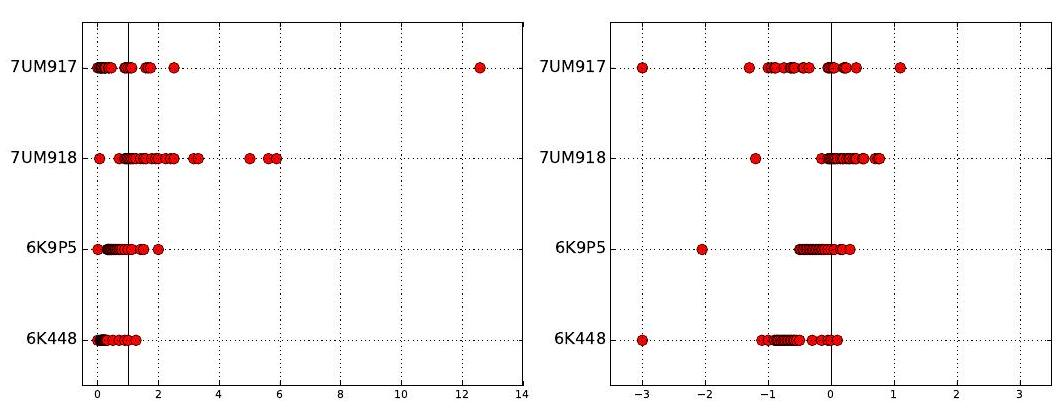
\includegraphics[max width=\textwidth]{2025_03_17_ca60ec0bfd96dcf8e028g-066}
    \caption{Plotting ratios on a scale cramps the space allocated to small ratios relative to large ratios (left). Plotting the logarithms of ratios better represents the underlying data (right).}
\end{figure}

यहाँ एक समाधान ज्यामितीय माध्य का उपयोग करना हो सकता था। लेकिन बेहतर है कि इन अनुपातों के लघुगणक को लिया जाए, ताकि वे समान विस्थापन प्रदान करें, क्योंकि $\log_{2}2=1$ और $\log_{2}(1 / 2)=-1$. हमें अतिरिक्त लाभ यह मिलता है कि एक इकाई अनुपात शून्य पर चित्रित होता है, इसलिए सकारात्मक और नकारात्मक संख्याएँ क्रमशः अनुचित और उचित अनुपातों के अनुरूप होती हैं।

मेरे छात्रों द्वारा अक्सर की जाने वाली एक नौसिखिया गलती में अनुपातों के मूल्यों की बजाय उनके लॉगरिदम्स का आरेखण शामिल होता है। चित्र 2.12 (बाएं) एक छात्र पत्र से लिया गया एक ग्राफ है, जो नए स्कोर का पुराने स्कोर के ऊपर अनुपात 24 घंटों के डाटा पर दर्शाता है (प्रत्येक लाल बिंदु एक घंटे का माप है) चार अलग-अलग डाटा सेट्स पर (प्रत्येक को एक पंक्ति दी गई है)। ठोस काली रेखा एक का अनुपात दर्शाती है, जहाँ दोनों स्कोर समान परिणाम देते हैं। अब इस ग्राफ को पढ़ने की कोशिश करें: यह आसान नहीं है क्योंकि रेखा के बाईं ओर बिंदु एक संकीर्ण पट्टी में एक साथ जमा हुए हैं। जो चीज उभर कर सामने आती है वह असामान्य डेटा है। निश्चित रूप से नया एल्गोरिदम शीर्ष पंक्ति में 7UM917 पर भयंकर रूप से प्रदर्शन करता है: दाईं ओर जाने वाला वह बिंदु वास्तव में एक असामान्य डेटा बिंदु है।\index{bell-shaped!distribution}\index{good scoring functions}\index{PageRank}\index{random variable!class rank}\index{random variable!search results}\index{random variable!top sports teams}\index{random variable!university rankings}\index{scores vs. rankings}

हालांकि ऐसा नहीं है। अब चित्र 2.12 (दाएं) पर देखें, जहां हम अनुपातों के लघुगणक को चित्रित करते हैं। काले रेखा के बाएं और दाएं समर्पित स्थान अब बराबर हो सकता है। और यह दिखाता है कि यह बिंदु वास्तव में इतना असाधारण नहीं था। सबसे बाईं ओर के बिंदुओं में सुधार की मात्रा दाईं ओर के बिंदुओं की तुलना में कहीं अधिक है। यह चित्रण प्रकट करता है कि नया एल्गोरिदम सामान्यतः चीजों को बेहतर बनाता है, केवल इसलिए कि हम अनुपात के स्थान पर अनुपात के लघुगणक दिखा रहे हैं।

% Mismatched: \sectionname{Logarithms and Normalizing Skewed Distributions}

वेरिएबल्स जो सममित, घंटी के आकार के वितरणों का पालन करते हैं, मॉडलों में विशेषताओं के रूप में अच्छे होते हैं। वे महत्वपूर्ण विविधता दिखाते हैं, इसलिए उन्हें चीजों के बीच अंतर करने के लिए प्रयोग किया जा सकता है, लेकिन इतने व्यापक पैमाने पर नहीं कि आउटलेयर भारी पड़ जाएं।

लेकिन हर वितरण सममित नहीं होता। चित्र 2.13 में दिखाए गए वितरण पर विचार करें।

\begin{figure}[h]
    \centering
    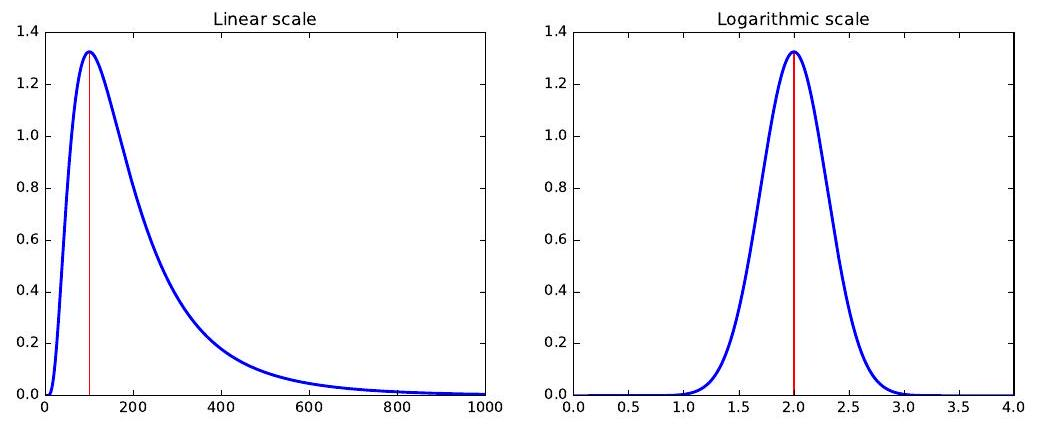
\includegraphics[max width=\textwidth]{2025_03_17_ca60ec0bfd96dcf8e028g-067}
    \caption{Hitting a skewed data distribution (left) with a $\log$ often yields a more bell-shaped distribution (right).}
\end{figure}

दाईं ओर की पूंछ बाईं ओर की पूंछ की तुलना में बहुत दूर जाती है। और हम पावर लॉज़ पर चर्चा करते समय, अनुभाग 5.1.5 में, और भी अधिक असंतुलित वितरण देखने के लिए निश्चित हैं। धन ऐसे वितरण का प्रतिनिधित्व करता है, जहाँ सबसे गरीब इंसान के पास शून्य या शायद नकारात्मक धन है, औसत व्यक्ति (आशावादी रूप से) हजारों डॉलर में है, और बिल गेट्स इस लेखन के समय\$100 बिलियन की ओर बढ़ रहे हैं।

हमें ऐसी वितरणों को कुछ आसान बनाने के लिए सामान्यीकरण की आवश्यकता है। एक पावर लॉ वितरण की घंटी बजाने के लिए हमें कुछ गैर-रेखीय चाहिए, जो बड़े मानों को अधिक मामूली मानों की तुलना में असंतुलित रूप से कम कर दे।

लघुगणक शक्ति कानून चरों के लिए पसंदीदा रूपांतरण है। अपनी लंबी पूंछ वाली वितरण को लॉग से मारो और अक्सर अच्छी चीजें होती हैं। आरेख 2.13 में वितरण \textit{लॉग नॉर्मल} वितरण है, इसलिए लघुगणक लेने से दाईं ओर एक उत्तम घंटी-आकृति वक्र प्राप्त हुआ। शक्ति कानून वितरण के साथ चर का लघुगणक लेना उन्हें पारंपरिक वितरणों के साथ अधिक संगत बनाता है। उदाहरण के लिए, एक उच्च-मध्यम वर्गीय पेशेवर के रूप में, मेरी संपत्ति लगभग मेरे भूखे छात्रों से उतने ही लॉग दूर है जितना कि मैं बिल गेट्स से हूँ!

कभी-कभी लॉगरिदम लेना बहुत ही कठोर कदम साबित होता है, और वर्गमूल जैसे कम नाटकीय गैर-रैखा रूपांतरण वितरण को सामान्य करने के लिए बेहतर काम करता है। सबसे अच्छा परीक्षण यह है कि रूपांतरित मानों की आवृत्ति वितरण की ग्राफ बनाएँ और देखें कि क्या यह घंटी के आकार का दिखता है: मोटे तौर पर सममित, बीच में उभार के साथ। तभी आपको पता चलता है कि आपके पास सही फंक्शन है।\index{normalization}\index{Z-score}

% Mismatched: \chaptername{War Story: Fitting Designer Genes}

शब्द \textit{बायोइन्फॉर्मैटिशियन} \index{bioinformatician} जीवन विज्ञान में "डेटा वैज्ञानिक" के लिए कहा जाता है, जो एक उभरते हुए अनुशासन के प्रवर्तक होते हैं जो डीएनए अनुक्रम डेटा के बड़े संकलनों का अध्ययन करके पैटर्न तलाशते हैं। अनुक्रम डेटा के साथ काम करना बहुत रोचक होता है, और मैं मानव जीनोम परियोजना की बहुत शुरुआत से शोध परियोजनाओं में ⸨बायोइन्फॉर्मैटिशियन⸩ की भूमिका निभा रहा हूँ।

डीएनए अनुक्रम चार-अक्षर वर्णमाला\textit{\{A, C, G, T\}} पर आधारित स्ट्रिंग्स होते हैं। प्रोटीन वह सामग्री बनाते हैं जिससे हम भौतिक रूप से निर्मित होते हैं, और ये 20 विभिन्न प्रकार की आणविक इकाइयों की स्ट्रिंग्स से मिलकर बनते हैं, जिन्हें एमिनो एसिड्स कहा जाता है। \textit{जीन्स} वे डीएनए अनुक्रम होते हैं जो यह बताने के लिए होते हैं कि कैसे विशिष्ट प्रोटीन बनाए जाते हैं, जिनमें से प्रत्येक इकाई को \textit{कोडॉन} नामक {\\textit{A, C, G, T\}} की तिकड़ी द्वारा वर्णित किया जाता है।

हमारे उद्देश्यों के लिए, यह जान लेना पर्याप्त है कि जीनों का वर्णन करने वाले डीएनए अनुक्रमों की एक विशाल संख्या होती है जो किसी विशेष वांछित प्रोटीन अनुक्रम के लिए \textit{कोड} कर सकते हैं। लेकिन उनमें से केवल एक का \textit{उपयोग} होता है। मेरे जीवविज्ञानी सहयोगी और मैं यह जानना चाहते थे कि क्यों।

मूल रूप से, यह माना गया था कि ये सभी विभिन्न पर्यायवाची एनकोडिंग मूलतः समान थीं, लेकिन अनुक्रम डेटा पर किए गए सांख्यिकी ने यह स्पष्ट कर दिया कि कुछ कोडन्स दूसरों की तुलना में अधिक बार उपयोग किए जाते हैं। जैविक निष्कर्ष यह है कि "कोडन्स मायने रखते हैं," और इसके अच्छे जैविक कारण हैं कि यह ऐसा होना चाहिए।

हम इस बात में दिलचस्पी लेने लगे कि "कोडन के पड़ोसी युग्म महत्व रखते हैं या नहीं।" शायद कुछ तिकड़ी युग्म तेल और पानी की तरह होते हैं, और मिलकर रहना उन्हें पसंद नहीं होता। अंग्रेज़ी में भी कुछ अक्षर युग्मों की क्रम वरीयता होती है: आप द्विवर्ण\textit{घ}को\textit{हग}से कहीं अधिक बार देखते हैं। शायद यह डीएनए में भी सही है? अगर ऐसा है, तो डीएनए अनुक्रम डेटा में कुछ तिकड़ी युग्म कम प्रतिनिधित्वित होने चाहिए।

इसका परीक्षण करने के लिए, हमें एक अंक की आवश्यकता थी जो यह तुलना करे कि हम एक विशेष तिकड़ी (जैसे\textit{x = CAT}) को दूसरे विशेष तिकड़ी (जैसे\textit{y = GAG}) के साथ कितना बार वास्तव में देखते हैं, इसकी तुलना में जो संयोग से अपेक्षित होता है।$F(xy)$को$xy$की आवृत्ति कहा जाए, डीएनए अनुक्रम डेटाबेस में$x$कोडन के बाद$य$कोडन कितनी बार वास्तव में देखा जाता है। ये कोडन विशिष्ट अमीनो एसिड्स के लिए कोड करते हैं, जैसे$a$और$b$क्रमशः। अमीनो एसिड$a$के लिए, इसके द्वारा कोडित होने की संभावना$x$है$P(x)=F(x) / F(a)$, और इसी तरह$P(y)=F(y) / F(b)$। तब$xy$को देखने की अपेक्षित संख्या होती है\index{Social Network–movie}

\[ 
\text{Expected}(xy) = \left(\frac{F(x)}{F(a)}\right)\left(\frac{F(y)}{F(b)}\right) F(ab) 
\]

इस आधार पर, हम किसी भी दिए गए हेक्सामर$xy$के लिए एक कोडन जोड़ी स्कोर की गणना कर सकते हैं:

\[ 
CPS(xy) = \ln \left( \frac{\text{Observed}(xy)}{\text{Expected}(xy)}\right) = \ln \left( \frac{F(xy)}{\frac{F(x) F(y)}{F(a) F(b)} F(ab)} \right) 
\]

इस अनुपात के लोगारिथ्म को लेने से बहुत अच्छी विशेषताएँ उत्पन्न हुईं। सबसे महत्वपूर्ण बात यह थी कि स्कोर का चिह्न अत्यधिक-प्रतिनिधि जोड़ों को कम-प्रतिनिधि जोड़ों से अलग करता था। क्योंकि मात्राएँ सममित थीं\(+1\)उतनी ही प्रभावशाली थी जितनी\(-1\)हम इन स्कोरों को जोड़ सकते थे या औसत निकाल सकते थे एक समझदारी पूर्ण तरीके से, और प्रत्येक जीन के लिए एक स्कोर दे सकते थे। हमने इन स्कोरों का उपयोग उन जीनों को डिज़ाइन करने के लिए किया जो वायरस के लिए बुरा होना चाहिए, जिसने टीके बनाने के लिए एक रोमांचक नई तकनीक दी।

\begin{center}
\begin{tabular}{|l|l|l|l|l|}
\hline
Fr. Dep. & Score &  & Fr. Ind. & Score \\
\hline
CATAGG & -1.74 &  & GGGGGG & -1.01 \\
\hline
TCTAGC & -1.61 &  & CCCCCC & -0.95 \\
\hline
GTTAGG & -1.58 &  & GGCGCC & -0.66 \\
\hline
GCTAGT & -1.48 &  & GGGGGT & -0.63 \\
\hline
CCTAGT & -1.44 &  & CGGGGG & -0.59 \\
\hline
GGTAGG & -1.41 &  & AGGGGG & -0.58 \\
\hline
CTTAGG & -1.40 &  & CACGTG & -0.58 \\
\hline
ACTAGC & -1.38 &  & ACCCCC & -0.56 \\
\hline
GCTAGC & -1.37 &  & GGGCCC & -0.56 \\
\hline
GCTAGA & -1.36 &  & CCCCCT & -0.53 \\
\hline
CCTAGC & -1.35 &  & CGCCCC & -0.52 \\
\hline
GATAGG & -1.35 &  & CCCCCG & -0.51 \\
\hline
\end{tabular}
\end{center}

\begin{figure}[h]
    \centering
    \caption{Patterns in DNA sequences with the lowest codon pair scores become obvious on inspection. When interpreted in-frame, the stop symbol TAG is substantially depleted (left). When interpreted in the other two frames, the most avoided patterns are all very low complexity, like runs of a single base (right).}
\end{figure}

यह जानना कि कुछ कोडॉन के जोड़े खराब थे,\textit{क्यों}वे खराब थे, यह स्पष्ट नहीं करता था। लेकिन दो संबंधित स्कोर (विवरण अप्रासंगिक) की गणना करके और त्रिकों को उनके आधार पर छांटकर, जैसा कि चित्र 2.14 में दिखाया गया है, कुछ पैटर्न उभर कर सामने आए। क्या आप पैटर्न देख रहे हैं? बाईं ओर सभी खराब अनुक्रमों में\textit{TAG}शामिल है, जो एक विशेष कोडॉन होता है जो जीन को रोकने के लिए बताता है। और दाईं ओर सभी खराब अनुक्रम बहुत ही सरल रिपीट होने वाले अनुक्रमों में\textit{C}और\textit{G}से मिलकर बनते हैं। ये जैविक रूप से यह समझाते हैं कि क्यों ये पैटर्न प्राकृतिक चयन द्वारा टाले जाते हैं, जिसका अर्थ है कि हमने जीवन के बारे में कुछ बहुत सार्थक खोज किया है।

इस कहानी से हमें दो महत्वपूर्ण पाठ मिलते हैं। पहला, आइटम के विशिष्ट पहलुओं को उजागर करने के लिए संख्यात्मक स्कोरिंग फंक्शन्स विकसित करना बहुत उपयोगी हो सकता है ताकि पैटर्न प्रकट हो सकें। वास्तव में, अध्याय 4 ऐसे सिस्टम्स के विकास पर ध्यान केंद्रित करेगा। दूसरा, इन मात्राओं पर लॉगरिदम का उपयोग करना उन्हें और भी उपयोगी बना सकता है, जिससे हम पूरे दृश्य को बेहतर तरीके से देख सकें।

% Mismatched: \chaptername{Chapter Notes}

संभाव्यता सिद्धांत के लिए कई उत्कृष्ट परिचय उपलब्ध हैं, जिनमें \cite{tijms2012understanding, bertsekas2008introduction} शामिल है। प्राथमिक सांख्यिकी के लिए भी यही स्थिति है, जिसमें अच्छे परिचयात्मक पाठ \cite{james2013introduction, wheelan2013naked} शामिल हैं। इस अध्याय में संभाव्यता सिद्धांत का संक्षिप्त इतिहास Weaver \cite{weaver1982lady} पर आधारित है।

अपने सबसे मजबूत रूप में, कुशल बाजार परिकल्पना का कहना है कि सार्वजनिक जानकारी का उपयोग करके शेयर बाजार को मूल रूप से भविष्यवाणी नहीं किया जा सकता। मेरी व्यक्तिगत सलाह है कि आपको उन इंडेक्स फंड्स में निवेश करना चाहिए जो सक्रिय रूप से बाजार की दिशा को भविष्यवाणी करने का प्रयास नहीं करते। मैल्किल की \textit{A Random Walk Down Wall Street}\cite{malkiel1999random}\index{Borda’s method}\index{rankings!merging}

%---- Page End Break Here ---- Page : 52

% Page : 52
\noindent
is an excellent introduction to such investment thinking.\\
The Fast Fourier Transform (FFT) provides an $O(n \log n)$ time algorithm to compute the full autocorrelation function of an $n$-element sequence, where the straightforward computation of $n$ correlations takes $O\left(n^{2}\right)$. Bracewell \cite{bracewell1999fourier} and Brigham \cite{brigham1988fast} are excellent introductions to Fourier transforms and the FFT. See also the exposition in Press et.al. \cite{press2007numerical}.

चित्र 2.10 में कॉमिक स्ट्रिप रैंडल मुनरो के वेबकॉमिक\textit{xkcd} से ली गई है, विशेष रूप से \href{https://xkcd.com/552}{https://xkcd.com/552}, और इसे अनुमति के साथ पुनर्मुद्रित किया गया है।

अनुभाग 2.5 की युद्ध कहानी हमारे इस कार्य के इर्द-गिर्द घूमती है कि कैसे कोडॉन पेयर पक्षपात की घटना जीन अनुवादन को प्रभावित करती है। चित्र 2.14 मेरे सहकर्मी जस्टिन गार्डिन से आता है। पोलियो और फ्लू जैसी वायरल रोगों के लिए टीके डिजाइन करने के लिए हमने कोडॉन पेयर पक्षपात का कैसे उपयोग किया, इस पर चर्चा के लिए [CPS$^{+}$08, MCP$^{+}$10, \cite{skiena2012redesigning}] देखें।

\section{अभ्यास}
% असंगत: \subsectionname{Probability}

\begin{enumerate}
    \item[2-1.] \textbf{[3]} मान लीजिए कि $80\%$ लोग मूंगफली का मक्खन पसंद करते हैं, $89\%$ जैली पसंद करते हैं, और $78\%$ दोनों पसंद करते हैं। यदि एक यादृच्छिक रूप से चुना गया व्यक्ति मूंगफली का मक्खन पसंद करता है, तो इस बात की क्या संभावना है कि वह जैली भी पसंद करता है?
    \item[2-2.] \textbf{[3]} मान लीजिए कि $P(A)=0.3$ और $P(B)=0.7$।
    \begin{enumerate}
        \item क्या आप $P(A \text{ और } B)$ की गणना कर सकते हैं यदि आपको केवल $P(A)$ और $P(B)$ पता है?
        \item मान लीजिए कि घटनाएँ $A$ और $B$ स्वतंत्र यादृच्छिक प्रक्रियाओं से उत्पन्न होती हैं:
        \begin{itemize}
            \item $P(A \text{ और } B)$ क्या है?
            \item $P(A \text{ या } B)$ क्या है?
            \item $P(A \mid B)$ क्या है?
        \end{itemize}
    \end{enumerate}

\item[2-3.]\textbf{[3]} कल्पना कीजिए एक खेल की जहाँ आपका स्कोर दो पासों के अधिकतम मान के बराबर है। प्रत्येक घटना की संभावना की गणना करें$\{1,\ldots, 6\}$। 
\item[2-4.]\textbf{[8]} सिद्ध करें कि एक यादृच्छिक चर$X$से खींचे गए जोड़ी मानों के अधिकतम का संचयी वितरण फलन$X$के मूल संचयी वितरण फलन का वर्ग है। 
\item[2-5.]\textbf{[5]} यदि दो द्विआधारी यादृच्छिक चर$X$और$Y$ स्वतंत्र हैं, तो क्या$\bar{X}$($X$ का पूरक) और$Y$ भी स्वतंत्र हैं? प्रमाण दें या एक विपरीत उदाहरण प्रस्तुत करें। 

\index{directed acyclic graph}\index{topological sorting}
\subsection{सांख्यिकी}

\begin{enumerate}
    \item[2-6.] \textbf{[3]} प्रत्येक वितरण की जोड़ी की तुलना करें ताकि यह निर्णय लिया जा सके कि किसका माध्य और मानक विचलन अधिक है। आपको $\mu$ और $\sigma$ के वास्तविक मानों की गणना करने की आवश्यकता नहीं है, बस यह देखना है कि वे एक-दूसरे की तुलना में कैसे हैं।
    \begin{enumerate}
        \item i. $3,5,5,5,8,11,11,11,13$.
        \item ii. $3,5,5,5,8,11,11,11,20$.
        \item i. $-20,0,0,0,15,25,30,30$.
        \item ii. $-40,0,0,0,15,25,30,30$.
        \item i. $0,2,4,6,8,10$.
        \item ii. $20,22,24,26,28,30$.
        \item i. $100,200,300,400,500$.
        \item ii. $0,50,300,550,600$.
    \end{enumerate}

\item[2-7.]\textbf{[3]}ऐसी संभावना वितरण का निर्माण करें जहां कोई द्रव्यमान माध्य के एक $\sigma$ के भीतर न हो।
\item[2-8.]\textbf{[3]}यादृच्छिक पूर्णांकों पर अंकगणितीय और ज्यामितीय माध्य की तुलना कैसे होती है?
\item[2-9.]\textbf{[3]}दिखाएँ कि जब सभी पद समान होते हैं तो अंकगणितीय माध्य ज्यामितीय माध्य के बराबर होता है।
\end{enumerate}

% Mismatched: \subsectionname{Correlation Analysis}

\begin{enumerate}
    \item[2-10.] \textbf{[3]} सही या गलत: -0.9 का सहसंबंध गुणांक 0.5 के सहसंबंध गुणांक की तुलना में एक मजबूत रैखिक संबंध को इंगित करता है। क्यों समझाएं।
    \item[2-11.] \textbf{[3]} दिए गए कंपनी में कॉलेज और हाई स्कूल स्नातकों की वार्षिक तनख्वाहों के बीच सहसंबंध गुणांक क्या होगा, यदि प्रत्येक संभावित नौकरी शीर्षक के लिए कॉलेज स्नातक हमेशा बनाते:
    \begin{enumerate}
        \item $\$5,000$ हाई स्कूल ग्रेड्स से अधिक?
        \item $25\%$ हाई स्कूल ग्रेड्स से अधिक?
        \item $15\%$ हाई स्कूल ग्रेड्स से कम?
    \end{enumerate}

\item[2-12.]\textbf{[3]}अगर पुरुष हमेशा ऐसी महिलाओं से विवाह करते हैं जिनकी उम्र:

\begin{enumerate}
        \item अपने से तीन साल छोटे?
        \item अपने से दो साल बड़े?\index{Clyde}\index{National Football League}\index{point spread}
        \item अपने उम्र के आधे?
    \end{enumerate}

\item[2-13.]\textbf{[5]}गूगल खोज में पाए गए डाटा या साहित्य का उपयोग करके इनके बीच सहसंबंध की ताकत का अनुमान/मापन करें:\index{football!game prediction}

\begin{enumerate}
        \item बेसबॉल में हिट्स और वॉक्स स्कोर करने वाले हिटर्स के लिए।
        \item बेसबॉल में पिचर्स द्वारा अनुमति दी गई हिट्स और वॉक्स।
    \end{enumerate}

\item[2-14.]\textbf{[5]}समान रूप से खींचे गए बिंदुओं के नमूनों के लिए पीयरसन और स्फीयरमेन रैंक सहसंबंधों की गणना करें$(x, x^{k})$। जैसे-जैसे$k$बढ़ता है, यह मान कैसे बदलते हैं?
\end{enumerate}

% Mismatched: \subsectionname{Logarithms}

\begin{enumerate}
    \item[2-15.] \textbf{[3]} यह दिखाएँ कि 1 से कम किसी भी संख्या का लॉगरिद्म ऋणात्मक होता है।
    \item[2-16.] \textbf{[3]} यह दिखाएँ कि शून्य का लॉगरिद्म अपरिभाषित होता है।
    \item[2-17.] \textbf{[5]} यह सिद्ध करें कि
    \[
    x \cdot y = b^{(\log_{b} x + \log_{b} y)}
    \]
    \item[2-18.] \textbf{[5]} यह सिद्ध करें कि किसी base-$b$ के लॉगरिद्म को base-$a$ में बदलने के सूत्र की सहीता, कि
    \[
    \log_{a}(x) = \frac{\log_{b}(x)}{\log_{b}(a)}
    \]
\end{enumerate}

\subsection{कार्यान्वयन परियोजनाएँ}

\begin{enumerate}
    \item[2-19.] \textbf{[3]} कुछ दिलचस्प डेटा सेट खोजें, और तुलना करें कि उनके माध्य और मध्य के कितने समान हैं। वे कौन से वितरण हैं जहाँ माध्य और मध्य सबसे अधिक भिन्न होते हैं?
    \item[2-20.] \textbf{[3]} कुछ दिलचस्प डेटा सेट खोजें और सभी जोड़ों में दिलचस्प सहसंबंध खोजें। शायद \href{http://www.data-manual.com/}{http://www.data-manual.com/} पर उपलब्ध डेटा से शुरू करें। आपको क्या मिलता है?
\end{enumerate}

\subsection{साक्षात्कार प्रश्न}

\begin{enumerate}
    \item[2-21.] \textbf{[3]} एक सिक्के के $n$ बार उछाल पर ठीक $k$ बार हेड्स (शीर्ष) प्राप्त करने की संभावना क्या है, जहां प्रत्येक उछाल पर हेड्स आने की संभावना $p$ है? $k$ या उससे अधिक हेड्स के बारे में क्या?
    \item[2-22.] \textbf{[5]} मान लीजिए कि एक लगातार बदलते सिक्के के $i$वें उछाल पर हेड्स मिलने की संभावना $f(i)$ है। आप कैसे कुशलता से गिनकर ठीक $k$ हेड्स $n$ उछालों में प्राप्त करने की संभावना को गणना करेंगे?
    \item[2-23.] \textbf{[5]} एक बास्केटबॉल खेल के आधे समय में आपको दो संभावित चुनौतियों की पेशकश की जाती है:
    \begin{enumerate}
        \item तीन शॉट लें, और उनमें से कम से कम दो को सफल बनाएं।
        \item आठ शॉट लें, और उनमें से कम से कम पांच को सफल बनाएं।
    \end{enumerate}

कौन सी चुनौती चुननी चाहिए ताकि खेल जीतने की संभावना बेहतर हो?
\item[2-24.]\textbf{[3]}सिक्का दस बार उछालना आठ हेड्स और दो टेल्स का परिणाम देता है। आप यह कैसे विश्लेषण करेंगे कि क्या सिक्का निष्पक्ष है? $p$-मूल्य क्या है?
\item[2-25.]\textbf{[5]}$n$संख्याओं की एक धारा दी गई है, केवल स्थिर भंडारण का उपयोग करते हुए यादृच्छिक रूप से एक को कैसे चुनें। यदि आपको अग्रिम में$n$नहीं पता हो तो क्या करेंगे?
\item[2-26.]\textbf{[5]}एक$k$-स्ट्रिक $i$उछाल में एक$n$सिक्का फ्लिपों के क्रम में शुरू होती है जब $i$वां फ्लिप और अगले$k-1$फ्लिप समान होते हैं। उदाहरण के लिए, HTTTHH क्रम में 2-स्ट्रिक दूसरा, तीसरा और पांचवां उछाल में शुरू होती है। निष्पक्ष सिक्के के$n$उछालों में आप कितने$k$-स्ट्रिक्स की अपेक्षा करेंगे देखेंगे?
\item[2-27.]\textbf{[5]}एक व्यक्ति बेतरतीब आठ-अंकीय संख्या एक पॉकेट कैलकुलेटर में टाइप करता है। संभावना क्या है कि संख्या उल्टा करने पर भी समान दिखेगी?
\item[2-28.]\textbf{[3]}आप एक पासा फेंकने का खेल खेलते हैं जिसमें आपके पास दो विकल्प हैं:

\begin{enumerate}
        \item पासा एक बार फेंकें और प्राप्त संख्या के बराबर ईनाम प्राप्त करें (जैसे, \$3 संख्या "3" के लिए) और फिर खेल को रोक दें।
        \item आप पहले ईनाम को उसके परिणाम के अनुसार अस्वीकार सकते हैं और पासा दूसरी बार फेंक सकते हैं, और उसी प्रकार से ईनाम प्राप्त कर सकते हैं।
    \end{enumerate}

किस रणनीति का चयन आपको आपका इनाम अधिकतम देगा? अर्थात, पहले रोल के किन परिणामों के लिए आपको दूसरा खेल खेलने का चुनाव करना चाहिए? यदि आप दूसरी रणनीति चुनते हैं, तो इनाम की सांख्यिकीय अपेक्षा क्या है?
\item[2-29.]\textbf{[3]}ए/बी परीक्षण क्या है और यह कैसे काम करता है?
\item[2-30.]\textbf{[3]}सांख्यिकीय स्वतंत्रता और सहसंबंध के बीच क्या अंतर है?
\item[2-31.]\textbf{[3]}हम अक्सर कहते हैं कि सहसंबंध कारणता को इंगित नहीं करता है। इसका क्या मतलब है?
\item[2-32.]\textbf{[5]}दिशात्मक वितरण और समान वितरण के बीच क्या अंतर है?
\end{enumerate}

\subsection{कागल चुनौती}

\begin{enumerate}
    \item[2-33.] कारण-प्रभाव जोड़े: सहसंबंध बनाम कारणता। \href{https://www.kaggle.com/c/cause-effect-pairs}{https://www.kaggle.com/c/cause-effect-pairs}
    \item[2-34.] "अनियमित संख्या" का पूर्वानुमान लगाएँ जो किसी अनुक्रम में अगला होगा। \href{https://www.kaggle.com/c/random-number-grand-challenge}{https://www.kaggle.com/c/random-number-grand-challenge}
    \item[2-35.] एक पालतू आश्रय में जानवरों के भाग्य का पूर्वानुमान लगाएँ। \href{https://www.kaggle.com/c/shelter-animal-outcomes}{https://www.kaggle.com/c/shelter-animal-outcomes}
\end{enumerate}

%---- Page End Break Here ---- Page : 56

\chapter{डेटा मंगिंग}

\epigraph{दो अवसरों पर मुझसे पूछा गया है, "प्रार्थना करें, मिस्टर बैबेज, अगर आप मशीन में गलत आँकड़े डालते हैं, तो क्या सही उत्तर निकलेंगे?" ... मैं उस प्रकार की विचारों की गड़बड़ी को सही से समझने में असमर्थ हूँ जो ऐसे प्रश्न को उत्पन्न कर सकती है।}{\index{R}-- \textit{चार्ल्स बैबेज}}

अधिकांश डेटा वैज्ञानिक अपना ज्यादातर समय डेटा को साफ और प्रारूपित करने में बिताते हैं। बाकी लोग अपना ज्यादातर समय यह शिकायत करने में बिताते हैं कि उनके पास वह करने के लिए कोई डेटा उपलब्ध नहीं है जो वे करना चाहते हैं।

इस अध्याय में, हम आंकड़ों के साथ गणना के कुछ मूल यांत्रिकी पर काम करेंगे। न कि उच्च-स्तरीय चीजें जैसे सांख्यिकी या मशीन लर्निंग, बल्कि आंकड़ों को ढूँढने और साफ करने का मूलभूत काम; इसे \textit{डेटा मन्जिंग} के नाम से जाना जाता है।

हालाँकि व्यावहारिक प्रश्न जैसे “सर्वश्रेष्ठ ⸨लाइब्रेरी⸩ या ⸨प्रोग्रामिंग लैंग्वेज⸩ कौन सा उपलब्ध है?” स्पष्ट रूप से महत्वपूर्ण हैं, लेकिन उनके उत्तर इतनी तेजी से बदलते हैं कि इस तरह की पुस्तक सही स्थान नहीं है जहां इन्हें संबोधित किया जा सके। इसलिए मैं इस पुस्तक को किसी विशेष ⸨सॉफ्टवेयर टूल्स⸩ के सेट के इर्द-गिर्द न बनाकर सामान्य सिद्धांतों के स्तर पर ही रहूँगा। फिर भी, हम इस अध्याय में उपलब्ध संसाधनों की भूमि-स्केप पर चर्चा करेंगे: वे क्यों मौजूद हैं, वे क्या करते हैं, और उनका सर्वोत्तम उपयोग कैसे किया जाए।

किसी भी डेटा विज्ञान परियोजना में पहला कदम सही डेटा प्राप्त करना होता है। लेकिन यह अक्सर परेशान करने वाला कठिन होता है। यह अध्याय डेटा संसाधनों के लिए सबसे समृद्ध शिकार क्षेत्रों का सर्वेक्षण करेगा, और फिर जिसे आप प्राप्त करते हैं उसे साफ़ करने की तकनीकों का परिचय देगा। आपके डेटा को संभालना ताकि आप इसे सुरक्षित रूप से विश्लेषण कर सकें, महत्वपूर्ण परिणामों के लिए आवश्यक है। जैसा कि बबैज स्वयं संक्षेप में कह सकता था, "गड़बड़ी अंदर, गड़बड़ी बाहर।"

\section{डेटा साइंस के लिए भाषाएँ}

सिद्धांत रूप में, प्रत्येक पर्याप्त शक्तिशाली प्रोग्रामिंग भाषा किसी भी एल्गोरिथ्म को व्यक्त करने में सक्षम होती है जो गणना के योग्य हो। लेकिन व्यवहार में, विशेष कार्यों पर कुछ प्रोग्रामिंग भाषाएँ अन्य की तुलना में अधिक बेहतर साबित होती हैं। यहाँ बेहतर मतलब हो सकता है\textit{प्रोग्रामर के लिए आसान}या शायद\textit{अधिक कम्प्यूटेशनल रूप से कुशल}, इस पर निर्भर करता है कि हाथ में मिशन क्या है।

उन मुख्य डेटा साइंस प्रोग्रामिंग भाषाओं के बारे में जानकारी रखें:



शायद Python के खिलाफ सबसे बड़ा तर्क उसकी दक्षता है: व्याख्यायित भाषाएँ संकलित भाषाओं की गति के साथ प्रतिस्पर्धा नहीं कर सकतीं। लेकिन Python संकलक कुछ हद तक मौजूद हैं, और गणनात्मक रूप से गहन कार्यों के लिए कुशल C/असेंबली भाषा पुस्तकालयों में लिंक करने का समर्थन करते हैं। अंतिम निष्कर्ष यह है कि इस पुस्तक में प्रस्तुत सामग्री के माध्यम से काम करने में Python शायद आपका मुख्य उपकरण होना चाहिए। 
  
\item\textit{पर्ल}:\index{Perl} यह\textit{प्रयुक्त}वेब पर डेटा मंगिंग के लिए प्रमुख भाषा होती थी, इसके पहले कि Python ने इसे पछाड़ दिया। TIOBE प्रोग्रामिंग भाषा लोकप्रियता सूचकांक (\href{http://www.tiobe.com/tiobe-index}{http://www.tiobe.com/tiobe-index}) में, पहली बार 2008 में Python ने पर्ल को लोकप्रियता में पार कर लिया और पीछे मुड़कर नहीं देखा। इसके कई कारण हैं, जिनमें ऑब्जेक्ट-ओरिएंटेड प्रोग्रामिंग के लिए अधिक मजबूत समर्थन और बेहतर उपलब्ध पुस्तकालय शामिल हैं, लेकिन अंतिम निष्कर्ष यह है कि इस समय पर्ल में परियोजनाएं शुरू करने के लिए कुछ अच्छे कारण हैं। हालांकि, यदि आप इसे किसी विरासत परियोजना में पाते हैं, तो आश्चर्यचकित न हों।

\item\textit{R}: यह सांख्यिकीविदों की प्रोग्रामिंग भाषा है, जिसमें डेटा विश्लेषण और दृश्य प्रस्तुति के लिए सबसे गहरी पुस्तकालयें उपलब्ध हैं। डेटा विज्ञान की दुनिया R और Python खेमों में बंटी हुई है, जिसमें R संभवतः खोज के लिए अधिक उपयुक्त हो सकता है और Python उत्पादन उपयोग के लिए बेहतर हो सकता है। R के साथ सहभागिता की शैली कुछ हद तक एक प्राप्त स्वाद है, इसलिए मैं आपको इसके साथ थोड़ा खेलकर यह देखने के लिए प्रोत्साहित करता हूँ कि क्या यह आपको स्वाभाविक लगता है।

लिंकजेस आर और पाइथन के बीच में मौजूद हैं, इसलिए आप पाइथन कोड में आसानी से आर लाइब्रेरी फंक्शन्स को कॉल कर सकते हैं। यह उन्नत सांख्यिकी तरीकों तक पहुंच प्रदान करता है, जिन्हें शायद नेटिव पाइथन लाइब्रेरीज़ द्वारा समर्थित नहीं किया जा सकता है।

\item\textit{मैटलैब}:\index{Matlab} यहां पर मैट का अर्थ \textit{मैट्रिक्स} है, क्योंकि मैटलैब एक भाषा है जो मैट्रिक्स के तेज और कुशल प्रबंधन के लिए बनाई गई है। जैसा कि हम देखेंगे, कई मशीन लर्निंग एल्गोरिदम मैट्रिक्स पर की जाने वाली क्रियाओं में सिमट जाते हैं, जिससे मैटलैब अधिकतम स्तर के अमूर्तन पर प्रोग्रामिंग करने वाले इंजीनियरों के लिए स्वाभाविक रूप से उपयुक्त विकल्प बन जाता है।

मैटलब एक मालिकाना प्रणाली है। हालाँकि, इसके कई कार्यात्मकताएँ जीएनयू ऑक्टेव में उपलब्ध हैं, जो एक ओपन-सोर्स विकल्प है। 
  
\item\textit{जावा और सी/सी++}: बड़े सिस्टमों के विकास के लिए ये मुख्यधारा की प्रोग्रामिंग भाषाएँ बड़ी डेटा अनुप्रयोगों में महत्वपूर्ण हैं। हडूप और स्पार्क जैसे पैरेलल प्रोसेसिंग सिस्टम क्रमशः जावा और सी++ पर आधारित होते हैं। यदि आप वितरित कंप्यूटिंग की दुनिया में रह रहे हैं, तो आप यहाँ सूचीबद्ध अन्य भाषाओं की बजाय जावा और सी++ की दुनिया में रह रहे हैं। 
  
\item\textit{मैथमैटिका/वोल्फ्राम अल्फा}: मैथमैटिका एक मालिकाना प्रणाली है जो संख्यात्मक और प्रतीकात्मक गणित के सभी पहलुओं के लिए संगणनात्मक सहायता प्रदान करती है, जो कम मालिकाना वोल्फ्राम प्रोग्रामिंग भाषा पर आधारित है। यह वोल्फ्राम अल्फा संगणनात्मक ज्ञान इंजन की नींव है, जो एल्गोरिदम और पहले से पचे डेटा स्रोतों के मिश्रण के माध्यम से प्राकृतिक भाषा-जैसे सवालों को संसाधित करता है। इसे \href{http://www.wolframalpha.com}{wolframalpha.com}.\index{exercises}\index{learning to rank} पर देख सकते हैं।

मैं इस बात को स्वीकार करूंगा कि मैथमेटिका के लिए मेरे दिल में एक गर्म स्थान है। यह वही है जिसे मैं तब चुनता हूँ जब मैं कोई छोटा डेटा विश्लेषण या सिमुलेशन कर रहा होता हूँ, लेकिन लागत ने पारंपरिक रूप से इसे कई उपयोगकर्ताओं की पहुँच से बाहर रखा है। शायद अब वोलफ्राम भाषा की रिलीज़ ने इसे एक बड़े समुदाय के लिए खोल दिया है।
  
\item\textit{एक्सेल}: स्प्रेडशीट प्रोग्राम जैसे एक्सेल एक्सप्लरेटरी डेटा विश्लेषण के लिए शक्तिशाली उपकरण हैं, जैसे कि दिए गए डेटा सेट के साथ यह देखने के लिए खेलना कि इसमें क्या शामिल है। इस प्रकार के अनुप्रयोगों के लिए वे हमारे सम्मान के पात्र हैं।

पूरा सुविधा सम्पन्न स्प्रेडशीट प्रोग्राम शक्तिशाली उपयोगकर्ताओं के लिए आश्चर्यजनक मात्रा में छिपी हुई कार्यक्षमता समेटे होते हैं। मेरे एक छात्र जो माइक्रोसॉफ्ट के उच्चाधिकारी बने, उन्होंने मुझे बताया कि Excel के लिए सभी नए फीचर अनुरोधों में से 25\% पहले से मौजूद कार्यक्षमता का प्रस्ताव करते हैं। जिन विशेष कार्यों और डेटा हेरफेर विशेषताओं की आपको जरूरत है, वे शायद Excel में पहले से ही मौजूद हैं यदि आप इसे ध्यान से देखें, उसी तरह से जिस तरह से एक Python लाइब्रेरी को आवश्यकता के अनुसार ढूंढने पर संभवतः पाएंगे।
\end{itemize}

\subsection{नोटबुक परिवेशों का महत्व}

डेटा साइंस प्रोजेक्ट के लिए मुख्य डिलिवरेबल कोई प्रोग्राम नहीं होना चाहिए। यह कोई डेटा सेट नहीं होना चाहिए। यह आपके डेटा पर प्रोग्राम चलाने के परिणाम नहीं होना चाहिए। यह सिर्फ एक लिखित रिपोर्ट भी नहीं होना चाहिए।

प्रत्येक डेटा साइंस परियोजना का निष्कर्षण परिणाम एक गणनीय नोटबुक होना चाहिए जो कोड, डेटा, गणनात्मक परिणाम, और आपने प्रक्रिया में जो सीखा उसका लेखन विश्लेषण एक साथ बाँधता हो। आकृति 3.1 एक Jupyter/IPython नोटबुक से एक अंश प्रस्तुत करती है, जो दिखाती है कि यह कोड, ग्राफिक्स, और प्रलेखन को वर्णनात्मक दस्तावेज़ में कैसे एकीकृत करता है जिसे एक प्रोग्राम की तरह निष्पादित किया जा सकता है।

यह इतना महत्वपूर्ण इसलिए है क्योंकि संगणकीय परिणाम पैरामीटर चयन और डिजाइन निर्णयों की लंबी श्रृंखलाओं का उत्पाद होते हैं। यह कई समस्याएं उत्पन्न करता है जिन्हें नोटबुक कम्प्यूटिंग वातावरण द्वारा हल किया जाता है:

\footnotetext{पूरी जानकारी: मैं स्टीफन वोलफ्रेम को तीस वर्षों से जानता हूँ। वास्तव में, हमने मिलकर आईपैड का आविष्कार किया है \cite{barron2010apple}.}

%---- Page End Break Here ---- Page : 59







\begin{verbatim}
degrees = range(1, 8)
errors = np.array([regressor3(d) for d in degrees])
plt.plot(degrees, errors[:, 0], marker='^', c='r', label='Testing samples')
plt.plot(degrees, errors[:, 1], marker='o', c='b', label='Training sample')
plt.yscale('log')
plt.xlabel("degree"); plt.ylabel("Error")
plt.legend(loc='best')
\end{verbatim}



डिग्री को स्वीप करके, हम मॉडल के प्रदर्शन के दो क्षेत्र खोजते हैं:

\begin{itemize}
  \item अंडरफिटिंग (डिग्री $\leq 3$): इसे इस तथ्य से पहचाना जाता है कि यदि हम मॉडल क्षमता बढ़ाते हैं तो परीक्षण त्रुटि कम हो जाएगी।
  \item ओवरफिटिंग (डिग्री $> 3$): इसे इस तथ्य से पहचाना जाता है कि परीक्षण त्रुटि बढ़ेगी यदि हम मॉडल क्षमता बढ़ाते हैं। ध्यान दें, कि प्रशिक्षण त्रुटि या तो कम हो रही है या वही रह रही है।
\end{itemize}

\subsection{मानक डेटा प्रारूप}
\index{data formats}
डेटा सभी प्रकार की जगहों से आता है, और सभी प्रकार के प्रारूपों में आता है। कौन सा प्रदर्श बेहतर है, यह इस पर निर्भर करता है कि अंतिम उपभोक्ता कौन है। चार्ट और ग्राफ़ आँकड़ों के अर्थ को व्यक्त करने के शानदार तरीके हैं। वास्तव में, अध्याय 6 डेटा को दृष्टिगत करने की तकनीकों पर केंद्रित होगा। लेकिन ये चित्र कंप्यूट करने के लिए डेटा के स्रोत के रूप में मूलतः व्यर्थ होते हैं। मुद्रित मानचित्रों से गूगल मैप्स तक पहुंचने में लंबा समय लगता है।

सबसे अच्छे संगणकीय डेटा प्रारूपों में कई उपयोगी गुण होते हैं:

\begin{itemize}
  \item \textit{वे कंप्यूटर द्वारा पार्स करने में आसान होते हैं:} उपयोगी प्रारूप में लिखा डेटा कहीं और फिर से इस्तेमाल करने के लिए होता है। परिष्कृत डेटा प्रारूप अक्सर एपीआईएस द्वारा समर्थित होते हैं जो तकनीकी विवरण को नियंत्रित करते हैं, यह सुनिश्चित करते हैं कि प्रारूप सही है।
  \item \textit{वे लोगों के लिए पढ़ने में आसान होते हैं:} डेटा को आंखों से जांचना कई संदर्भों में एक आवश्यक क्रिया है। इस निर्देशिका में से कौन सा डेटा फ़ाइल मेरे लिए उपयोग करने के लिए सही है? हम इस फ़ाइल में डेटा फ़ील्ड्स के बारे में क्या जानते हैं? प्रत्येक विशेष फ़ील्ड के लिए मूल्यों की मोटे तौर पर सीमा क्या है?\index{bell-shaped}\index{binomial distribution}\index{independence}\index{Pascal’s triangle}
\end{itemize}

ये उपयोग के मामले उस विशाल मूल्य की बात करते हैं जो एक डेटा फ़ाइल को टExt ऍडीटर में खोल कर उसे देखने से मिलता है। आमतौर पर, इसका मतलब है कि डेटा को मानवीय-पठनीय टेक्स्ट-एन्कोडेड प्रारूप में प्रस्तुत करना, जहां रिकॉर्ड्स को अलग-अलग पंक्तियों द्वारा चिन्हित किया जाता है, और फ़ील्ड्स को सीमांकन चिन्हों द्वारा अलग किया जाता है।\index{statistical distributions}

%---- Page End Break Here ---- Page : 61

\itemवे अन्य टूल्स और सिस्टेम द्वारा व्यापक रूप से उपयोग किए जाते हैं: स्वनिवेशी डेटा मानक को आविष्कार करने की इच्छा कॉर्पोरेट दिल में मजबूती से धड़कती है, और अधिकांश सॉफ्टवेयर डेवलपर किसी फ़ाइल प्रारूप के बजाय एक टूथब्रश साझा करना पसंद करेंगे। लेकिन ये आवेगों से दूर रहना चाहिए। डेटा की शक्ति अन्य डेटा संसाधनों के साथ इसे मिलाने और मैच करने से आती है, जिसे लोकप्रिय मानक प्रारूपों का उपयोग करके सबसे अधिक सुविधाजनक बनाया जाता है।
\end{itemize}

मैंने इस सूची में से एक गुण \textit{संक्षिप्तता} को बाहर रखा है, क्योंकि यह आमतौर पर आधुनिक कम्प्यूटिंग प्रणालियों पर चलने वाले अधिकांश अनुप्रयोगों के लिए प्राथमिक चिंता का विषय नहीं होता। डेटा भंडारण लागत को न्यूनतम करने की खोज अक्सर अन्य लक्ष्यों के विरुद्ध काम करती है। चतुराई से कई क्षेत्रों को पूर्णांकों के उच्च-आदेश वाले बिट्स में पैक करने से जगह बचती है, लेकिन यह इसे असंगत और पढ़ने योग्य नहीं बनाता।

सामान्य संपीड़न उपयोगिताएँ जैसे gzip मानव-मित्र फॉर्मेटिंग की अनावश्यकता को हटाने में अद्भुत रूप से अच्छी साबित होती हैं। डिस्क की कीमतें अविश्वसनीय रूप से सस्ती हैं: जैसा कि मैं यह लिख रहा हूँ, आप \$100 में लगभग 4TB ड्राइव खरीद सकते हैं, जो एक कड़ा प्रारूप प्रोग्रामिंग में बर्बाद होने वाले डेवलपर के एक घंटे की लागत से भी कम है। जब तक आप Facebook या Google के पैमाने पर संचालन नहीं कर रहे हैं, तब तक संक्षिप्तता का उतना महत्व नहीं है जितना आप सोच सकते हैं।\footnote{वास्तव में, Google में मेरे मित्र मुझे आश्वासन देते हैं कि वे अक्सर पेटाबाइट पैमाने पर भी स्थान के बारे में लापरवाह होते हैं।}

सबसे महत्वपूर्ण डेटा प्रारूप/प्रतिनिधित्व जिनके बारे में जानकारी होना आवश्यक है, नीचे चर्चा की गई है:

\begin{itemize}
  \item \textit{CSV (कॉमा सेपरेटेड वैल्यू)} फाइलें: ये फाइलें कार्यक्रमों के बीच डेटा विनिमय के लिए सबसे सरल, सबसे लोकप्रिय प्रारूप प्रदान करती हैं। कि प्रत्येक पंक्ति एक ही रेकॉर्ड का प्रतिनिधित्व करती है, जिसमें फील्ड्स को कॉमाओं से अलग किया जाता है, निरीक्षण से स्पष्ट है। लेकिन विशेष कैरेक्टर और टेक्स्ट स्ट्रिंग्स के चारों ओर बारीकियां घूमती हैं: अगर आपके नामों के बारे में डेटा में कोई कॉमा हो, जैसे "थर्स्टन हॉवेल, जूनियर।" तो \textit{csv} प्रारूप ऐसे कैरेक्टर को नॉन-डेलिमिटर के रूप में परख कोड करने के तरीके प्रदान करता है, लेकिन यह गंदा होता है। एक बेहतर विकल्प एक कम सामान्यता वाला डेलिमिटर कैरेक्टर का उपयोग करना है, जैसे कि \textit{tsv या टैब सेपरेटेड वैल्यू} फाइलों में।\\
यह जांचने का सबसे अच्छा तरीका कि आपकी \textit{csv} फाइल सही तरीके से फॉर्मेट की गई है, यह है कि माइक्रोसॉफ्ट एक्सेल या कुछ अन्य स्प्रेडशीट प्रोग्राम इसे बिना किसी समस्या के पढ़ सके। सुनिश्चित करें कि प्रत्येक प्रोजेक्ट के परिणाम इस परीक्षा को पास करते हैं जैसे ही पहला \texttt{csv} फाइल लिखी गई है, ताकि बाद में परेशानी न हो।
  \item \texttt{XML (एक्सटेंसिबल मार्कअप लैंग्वेज)}: संरचित लेकिन गैर-तालिका डेटा अक्सर एनोटेशनों के साथ एक टेक्स्ट के रूप में लिखा जाता है। टेक्स्ट के लिए एक नामित-इकाई टैगर का प्राकृतिक आउटपुट टेक्स्ट के प्रासंगिक उपस्ट्रिंग्स को ब्रैकेट में लपेटता है जो व्यक्ति, स्थान, या वस्तु को दर्शाता है। मैं यह पुस्तक लैटेक्स में लिख रहा हूँ, एक फॉर्मेटिंग भाषा में ब्रैकेटिंग कमांड होते हैं जो गणितीय अभिव्यक्तियों और \textbf{italicized text} के आसपास स्थित होते हैं। सभी वेबपेजों को ⸨HTML\end{itemize} में लिखा जाता है, हायपरटेक्स्ट मार्कअप लैंग्वेज में जो ब्रैकेटिंग कमांड का उपयोग करके डाक्यूमेंट्स को ⸨<b>⸩ और ⸨</b>⸩ जैसे ⸨bold faced text⸩ को घेरते हुए व्यवस्थित करता है।\\
⸨XML⸩ विशेष रूप से मार्कअप भाषाओं के विनिर्देशों को लिखने के लिए लागू भाषा है। एक उचित ⸨XML⸩ विनिर्देश उपयोगकर्ता को वह डाक्यूमेंट पढ़ने की क्षमता देता है जो विनिर्देश के अनुसार है। ऐसे विनिर्देशों को डिजाइन करने और पूरी तरह पालन करने की क्षमता प्रदान करता है।⸩

उनके प्रति अनुशासन आवश्यक है, लेकिन यह इसके लायक है। हमारी ल्यिडिया पाठ विश्लेषण प्रणाली के पहले संस्करण में, हमने अपने मार्कअप्स को "प्सूड़ो-XML" में लिखा, जिसे एड-हॉक पार्सर्स द्वारा पढ़ा गया जो दस्तावेजों के 99% को सही ढंग से संभालते थे लेकिन जब भी हम उन्हें विस्तारित करने की कोशिश करते थे, टूट जाते थे। दर्दनाक XML स्विच के बाद, सब कुछ अधिक भरोसेमंद\textit{और}अधिक कुशलता से काम करने लगा, क्योंकि हम तेजी से, ओपन-सोर्स XML पार्सर्स को तैनात कर सकते थे जो हमारी विशिष्टताओं को लागू करने के सभी कठिन कार्य को संभालते थे।

\begin{itemize}
  \item \textit{SQL (स्ट्रक्चर्ड क्वेरी लैंग्वेज) डेटाबेसेस}: स्प्रेडशीट्स स्वाभाविक रूप से डेटा की एकल तालिका के चारों ओर संरचित होती हैं। इसके विपरीत, रिलेशनल डेटाबेसेस कई विशिष्ट लेकिन संबंधित तालिकाओं को संशोधित करने में उत्कृष्ट साबित होती हैं, SQL का उपयोग करके एक कठिन लेकिन शक्तिशाली क्वेरी भाषा प्रदान करती हैं।\\
कोई भी उचित डेटाबेस सिस्टम रिकॉर्ड्स को csv या XML फाइलों के रूप में आयात और निर्यात करता है, साथ ही एक आंतरिक सामग्री डंप के रूप में। डेटाबेस में आंतरिक प्रतिनिधित्व अस्पष्ट होता है, इसलिए उन्हें एक डेटा प्रारूप के रूप में वर्णित करना वास्तव में सही नहीं होगा। फिर भी, मैं उन्हें यहां इसलिए जोर देता हूं क्योंकि SQL डेटाबेसेस \index{SQL databases}आमतौर पर कई डेटा फाइलों को एक असंगठित तरीके से संशोधित करने की तुलना में एक बेहतर और शक्तिशाली समाधान साबित होती हैं।
  \item \textit{JSON (जावास्क्रिप्ट ऑब्जेक्ट नोटेशन)}:\index{JSON} यह प्रोग्रामों के बीच डेटा ऑब्जेक्ट्स के प्रेषण के लिए एक प्रारूप है। यह एक प्रणाली से दूसरी प्रणाली तक वेरिएबल्स/डेटा संरचनाओं की स्थिति को संप्रेषित करने का एक स्वाभाविक तरीका है। यह प्रतिनिधित्व मूलतः वेरिएबल/फील्ड नामों से मेल खाते गुण-मूल्य जोड़ों की एक सूची है, और संबंधित मान:\index{financial market}\index{normal distribution!implications}\index{stock market}\index{Poisson distribution}
\end{itemize}

\begin{verbatim}
{"employees":[
    {"firstName":"John", "lastName":"Doe"},
    {"firstName":"Anna", "lastName":"Smith"},
    {"firstName":"Peter", "lastName":"Jones"}
]}
\end{verbatim}

क्योंकि उन आधुनिक प्रोग्रामिंग भाषाओं में पुस्Kथकालय функций उपलब्Dध हैं जो JSON ऑब्
젝트 पढ़ने और लिखने का समर्थन करती हैं, यह डेटा संरचनाओं को बाद में इस्तेमाल के लिए संग्रहीत करने का एक बहुत सुविधाजनक तरीका बन गया है। JSON ऑब्
젝트 मानव-पढ़नीय होती हैं, लेकिन वे काफी भ्रामक-दिखने वाली होती हैं, विशेष रूप से CSV फाइलों की तुलना में रिकॉर्ड्स की arrays को प्रदर्शित करते हुए। उन्हें जटिल संरचित ऑब्जект्स के लिए इस्तेमाल करें, लेकिन साधारण डेटा तालिकाओं के लिए नहीं।

\begin{itemize}
  \item \textit{प्रोटोकॉल बफर्स}: ये एक भाषा/प्लेटफ़ॉर्म-न्यूट्रल तरीका है जिसके द्वारा संरचित डेटा को संचार और संग्रहण के लिए सिरीअलाइज़ किया जाता है। ये XML (जहाँ आप अपनी संरचित डेटा का प्रारूप निर्धारित करते हैं) के हल्के संस्करण हैं, जिन्हें प्रोग्राम्स के बीच छोटे डेटा को संप्रेषित करने के लिए डिज़ाइन किया गया है, जैसे JSON। यह डेटा फॉर्मेट गूगल में इंटरमशीन कम्यूनिकेशन के लिए प्रयोग होता है। अपाचे थ्रिफ्ट एक संबंधित मानक है, जिसका प्रयोग फेसबुक में होता है।
\end{itemize}

%---- Page End Break Here ---- Page : 63

\begin{itemize}कुछ\end{itemize}

\section{डेटा एकत्रित करना}
किसी भी डेटा विज्ञान या मॉडलिंग परियोजना में सबसे महत्वपूर्ण मुद्दा सही डेटा सेट का चयन करना है। उपयुक्त डेटा स्रोतों की पहचान करना एक कला है, जो तीन मूलभूत प्रश्नों के इर्द-गिर्द घूमती है:

\begin{itemize}
  \item \textit{मेरे लिए आवश्यक डेटा वास्तव में किसके पास हो सकता है?}
  \item \textit{वे इसे मेरे लिए उपलब्ध कराने का क्यों निर्णय ले सकते हैं?}
  \item \textit{मैं इसे कैसे प्राप्त कर सकता हूँ?}
\end{itemize}

इस खंड में, हम इन प्रश्नों के उत्तरों का अन्वेषण करेंगे। हम डेटा के सामान्य स्रोतों पर नज़र डालेंगे, और आप संभवतः क्या पा सकते हैं और क्यों। इसके बाद हम एक्सेस प्राप्त करने के प्राथमिक तरीकों की समीक्षा करेंगे, जिसमें ए.पी.आई.s, स्क्रैपिंग, और लॉगिंग शामिल हैं।

\subsection{शिकार}
डेटा किसके पास है, और आप इसे कैसे प्राप्त कर सकते हैं? कुछ संभावित संदिग्धों की समीक्षा नीचे की गई है।

\subsubsection{कंपनियाँ और स्वामित्व डेटा स्रोत}
बड़े-बड़े कंपनियाँ जैसे फेसबुक, गूगल, अमेज़ॅन, अमेरिकन एक्सप्रेस, और ब्लू क्रॉस के पास उपयोगकर्ताओं और लेन-देन के बारे में अद्भुत मात्रा में रोमांचक डेटा होता है, जो दुनिया के संचालन को सुधारने के लिए इस्तेमाल किया जा सकता है। समस्या यह है कि बाहरी पहुँच प्राप्त करना आमतौर पर असंभव होता है। कंपनियाँ डेटा साझा करने के लिए अनिच्छुक होती हैं दो अच्छे कारणों के लिए:

\begin{itemize}
  \item \textit{व्यापार संबंधित मुद्दे}, और अपनी प्रतिस्पर्धा की मदद करने का डर।
  \item \textit{गोपनीयता संबंधित मुद्दे}, और अपने ग्राहकों को नाराज करने का डर।
\end{itemize}

एक दिल को छू लेने वाली कहानी है कि कॉर्पोरेट डेटा रिलीज़ के साथ क्या हो सकता है, जब एओएल ने शिक्षाविदों को अपने सर्च इंजन के लिए मिलियनों क्वेरीज़ का एक डेटा सेट प्रदान किया, जिसमें पहचान संबंधी जानकारी को सावधानीपूर्वक हटाया गया था। शिक्षाविदों ने सबसे पहले यह खोजा कि सबसे अधिक बार दर्ज की जाने वाली क्वेरीज़ अन्य सर्च इंजन जैसे गूगल की ओर भागने के लिए एक हताश प्रयास थी। इससे एओएल सर्च की गुणवत्ता में जनता का विश्वास बढ़ने के बजाय घट गया।

उनकी दूसरी खोज यह थी कि खोज क्वेरीज़ को गुमनाम करना पहले की अपेक्षा कहीं अधिक कठिन सिद्ध हुआ। बेशक आप उपयोगकर्ता नामों को आईडी नंबरों से बदल सकते हैं, लेकिन यह समझना उतना कठिन नहीं है कि \textit{Long Island} का वह व्यक्ति कौन है जो बार-बार \textit{Steven Skiena}, ⸨Stony Brook⸩ और \href{https://twitter.com/search?q=Skiena\&src=sprv}{https://twitter.com/search?q=Skiena\&src=sprv} के बारे में पूछताछ कर रहा है। वास्तव में, जैसे ही यह सार्वजनिक हुआ कि लोगों की पहचान इस डेटा रिलीज़ से उजागर हुई थी, जिम्मेदार पक्ष को निकाल दिया गया और डेटा सेट गायब हो गया। उपयोगकर्ता की गोपनीयता महत्वपूर्ण है, और डेटा साइंस के आसपास के नैतिक मुद्दों पर अनुभाग 12.7 में चर्चा की जाएगी।

इसलिए यह न सोचें कि आप कंपनियों को मीठी बातों में फंसाकर गोपनीय उपयोगकर्ता डेटा जारी करवाने जा रहे हैं। हालांकि, कई जिम्मेदार कंपनियां जैसे \textit{द न्यू यॉर्क टाइम्स}, ट्विटर, फेसबुक, और गूगल कुछ डेटा जारी करती हैं, आमतौर पर दर-सीमित एप्लिकेशन प्रोग्राम इंटरफेसेज़ \index{application program interfaces}(APIs) के माध्यम से। उनका आमतौर पर दो मकसद होता है:

\begin{itemize}
  \item ग्राहकों और तीसरे पक्ष को डेटा प्रदान करना जो बिक्री बढ़ा सकता है। उदाहरण के लिए, क्वेरी फ्रीक्वेंसी और विज्ञापन मूल्य निर्धारण के बारे में डेटा जारी करना अधिक लोगों को एक निश्चित मंच पर विज्ञापन देने के लिए प्रोत्साहित कर सकता है।
  \item यह आमतौर पर कंपनी के लिए अच्छा होता है कि वे सुचारू रूप से चलने वाले एपीआई प्रदान करें बजाय कि काउबॉय बार-बार उनकी साइट पर प्रहार करें और स्क्रैप करें।
\end{itemize}

इसलिए खंड 3.2.2 पर स्क्रैपिंग पढ़ने से पहले किसी सार्वजनिक एपीआई की तलाश करें। आपको बिल्कुल वही सामग्री या मात्रा नहीं मिलेगी जिसकी आप कल्पना कर रहे हैं, लेकिन शायद कुछ ऐसा जो शुरू करने के लिए पर्याप्त होगा। सीमाओं और उपयोग की शर्तों से अवगत रहें।

अन्य संगठन ऑफ़लाइन विश्लेषण के लिए रोचक डेटा का बड़े पैमाने पर डाउनलोड उपलब्ध कराते हैं, जैसा कि Google Ngrams, IMDb, और टैक्सी भाड़ा डेटासेट्स में चर्चा की गई है अध्याय 1 में। बड़े डेटा सेट अक्सर मूल्यवान मेटाडेटा के साथ आते हैं, जैसे पुस्तक शीर्षक, छवि विवरणिका, और संपादन इतिहास, जिनका सही कल्पना के साथ पुनः प्रयोजन किया जा सकता है।

अंततः, अधिकांश संगठन अपनी व्यापार से संबंधित आंतरिक डेटा सेट रखते हैं। एक कर्मचारी के रूप में, आपको वहां काम करते समय विशेष पहुंच मिलनी चाहिए। यह ध्यान में रखें कि कंपनियों की आंतरिक डेटा पहुंच नीति होती है, इसलिए आप अभी भी कुछ प्रतिबंधों के अधीन होंगे। इन नीतियों की शर्तों का उल्लंघन करना एक पूर्व-कर्मचारी बनने का उत्कृष्ट तरीका है।

\subsubsection{सरकारी डेटा स्रोत}
\index{government data}डेटा एकत्र करना उन महत्वपूर्ण कार्यों में से एक है जो सरकारें करती हैं। वास्तव में, संयुक्त राज्य अमेरिका की जनसंख्या की गणना करने की आवश्यकता हमारे संविधान द्वारा निर्धारित की गई है, और यह 1790 से हर दस साल के अंतराल पर अनुसूचित समय पर चल रही है।

शहर, राज्य, और संघीय सरकारें ओपन डेटा के प्रति अधिक प्रतिबद्ध हो गई हैं, ताकि नई अवसंरचनाओं की सुविधा प्रदान की जा सके और यह सुधारा जा सके कि सरकार अपनी मिशन को कैसे पूरा कर सकती है। वेबसाइट \href{http://Data.gov}{http://Data.gov} संघीय सरकार की पहल है, जो अपनी डेटा स्रोतों को केंद्रीय रूप से एकत्रित करने के लिए शुरू की गई है, और अंतिम गणना में यह 100,000 से अधिक डेटा सेट की ओर इशारा करती है!

सरकारी डेटा औद्योगिक डेटा से इस मायने में भिन्न होता है कि, सिद्धांततः, यह जनता का होता है। \textit{सूचना की स्वतंत्रता अधिनियम}\index{Freedom of Information Act}\index{Freedom of Information Act}(FOI) किसी भी नागरिक को किसी भी सरकारी दस्तावेज़ या डेटा सेट के लिए औपचारिक अनुरोध करने की अनुमति देता है। ऐसा अनुरोध एक प्रक्रिया शुरू करता है जिसके द्वारा यह निर्धारित किया जाता है कि क्या को जारी किया जा सकता है बिना राष्ट्रीय हित को नुकसान पहुँचाए या निजता का उल्लंघन किए बिना।

राज्य सरकारें पचास विभिन्न कानूनों के तहत काम करती हैं, इसलिए एक क्षेत्र में जो डेटा सख्ती से नियंत्रित होता है, वह दूसरों में स्वतंत्र रूप से उपलब्ध हो सकता है। न्यूयॉर्क जैसे प्रमुख शहरों में कई राज्यों की तुलना में बड़ा डेटा प्रोसेसिंग संचालन होता है, और यहाँ भी स्थान के अनुसार प्रतिबंध भिन्न होते हैं।

%---- Page End Break Here ---- Page : 65

% Ensuring correct chapter formatting

मैं सरकारी रिकॉर्ड्स के बारे में सोचने के निम्नलिखित तरीके की सिफारिश करता हूँ। अगर आप जो जानकारी खोज रहे हैं वह ऑनलाइन नहीं मिल रही है, तो पता लगाएँ कि कौन सी एजेंसी के पास वह हो सकती है। उनसे दोस्ताना तरीके से फोन करके पूछें कि क्या वे आपकी मदद कर सकते हैं। लेकिन अगर वे आपको रोकते हैं, तो बिना किसी संकोच के FOI एक्ट अनुरोध के लिए कोशिश करें। गोपनीयता को बनाए रखना आमतौर पर यह तय करने में सबसे बड़ी समस्या होती है कि किसी विशेष सरकारी डेटा सेट को जारी किया जा सकता है या नहीं।

\section{शैक्षणिक डेटा सेट}
ज्ञान के क्षेत्र में एक विशाल दुनिया है, जो मानवता के लिए महत्वपूर्ण मानी गई सभी चीजों को कवर करती है। शैक्षणिक अनुसंधान का एक बढ़ता हुआ हिस्सा बड़े डेटा सेट के निर्माण को शामिल करता है। कई पत्रिकाएँ अब प्रकाशन से पहले स्रोत डेटा को अन्य शोधकर्ताओं के लिए उपलब्ध कराने की आवश्यकता रखती हैं। यदि आप सही ढंग से खोजें, तो आप आर्थिक, चिकित्सा, जनसांख्यिकी, ऐतिहासिक, और वैज्ञानिक डेटा की विशाल मात्रा को खोजने की उम्मीद कर सकते हैं।\index{monotonic!sampling}\index{sampling!beyond one dimension}

इन डेटा सेट्स को खोजने की कुंजी है संबंधित पत्रिकाओं को ढूंढना। लगभग किसी भी रुचिकर विषय पर एक शैक्षणिक साहित्य होता है। गूगल स्कॉलर शोध प्रकाशनों का सबसे सुलभ स्रोत है। विषय के अनुसार खोजें, और शायद "ओपन साइंस" या "डेटा"। शोध प्रकाशन आम तौर पर इशारे देंगे कि संबंधित डेटा कहाँ पाया जा सकता है। यदि नहीं, तो लेखक से सीधे अनुरोध के साथ संपर्क करके जल्द ही इच्छित परिणाम प्राप्त किया जा सकता है।

प्रकाशित डेटा सेट का उपयोग करने की सबसे बड़ी परेशानी यह है कि किसी और ने पहले ही उन पर मेहनत करके उनका विश्लेषण किया हुआ होता है, इसलिए ये पहले से खनन किए गए स्रोत शायद दिलचस्प नए परिणामों से खाली हो चुके हों। लेकिन पुराने डेटा के लिए नए प्रश्न लाना आमतौर पर नई संभावनाओं को खोलता है।

अक्सर दिलचस्प डाटा साइंस प्रोजेक्ट्स में विभिन्न विषयों के शोधकर्ताओं के बीच सहयोग शामिल होता है, जैसे कि सामाजिक और प्राकृतिक विज्ञान। ये लोग आपसे अलग भाषा बोलते हैं, और शुरू में डराने वाले लग सकते हैं। लेकिन वे अक्सर सहयोग का स्वागत करते हैं, और जब आप शब्दावली को समझ लेते हैं तो आमतौर पर उनके मुद्दों को एक संतोषजनक स्तर पर समझना संभव होता है बिना विशेष अध्ययन के। विश्वास रखें कि अन्य विषयों के लोग आम तौर पर आपसे अधिक बुद्धिमान नहीं होते।

\section{स्वेट इक्विटी}
कभी-कभी आपको अपने डेटा के लिए मेहनत करनी पड़ सकती है, बजाय इसके कि आप इसे दूसरों से ले लें। बहुत सा ऐतिहासिक डेटा अभी भी केवल पुस्तकों या अन्य कागजी दस्तावेजों में ही मौजूद है, जिसे मैनुअल एंट्री और क्यूरेशन की आवश्यकता होती है। एक ग्राफ या तालिका में वह जानकारी हो सकती है जिसकी हमें आवश्यकता है, लेकिन एक पीडीऍफ़ (पोर्टेबल डॉक्यूमेंट फॉर्मेट) फ़ाइल में बंद ग्राफ़िक्स से नंबर निकालना कठिन हो सकता है।

मैंने देखा है कि संगणना-उन्मुख लोग आमतौर पर मैन्युअल डेटा प्रविष्टि करने में लगने वाले प्रयास को बहुत अधिक समझते हैं। एक रिकॉर्ड प्रति मिनट पर, आप आसानी से केवल दो कार्य दिवसों में 1,000 रिकॉर्ड दर्ज कर सकते हैं। इसके बजाय, संगणना लोग इस तरह के थकाने वाले काम से बचने के लिए बड़े प्रयास करते हैं, जैसे कि ऑप्टिकल कैरेक्टर रिकग्निशन (OCR) सिस्टम की तलाश करना जो फ़ाइल को गड़बड़ न करे, या एक शोर भरे स्कैन को साफ करने में अधिक समय बिताना जितना कि इसे फिर से टाइप करने में लगता।\index{Cohen’s d}\index{effect size}\index{correlation and causation}\index{statistical significance}

यहाँ एक बीच का रास्ता यह है कि आप किसी और को आपके लिए गंदा काम करने के लिए भुगतान करें। क्राउडसोर्सिंग प्लेटफॉर्म जैसे कि एमेज़ॅन टर्क \index{Amazon Turk}और क्राउडफ्लॉवर आपको लोगों की सेनाओं को भुगतान करने में सक्षम बनाते हैं ताकि वे आपकी मदद कर सकें डेटा निकालने में, या इसे पहली बार में इकट्ठा करने में। मानवीय टिप्पणियों की आवश्यकता वाले कार्य जैसे कि छवियों को लेबल करना या सर्वेक्षणों के उत्तर देना खासतौर पर दूरस्थ कार्यकर्ताओं के उपयोग के अच्छे उदाहरण हैं। क्राउडसोर्सिंग पर विस्तृत रूप से चर्चा अनुभाग 3.5 में की जाएगी।

कई अद्भुत ओपन डेटा संसाधनों का निर्माण योगदानकर्ताओं की टीमों द्वारा किया गया है, जैसे विकिपीडिया, फ़्रीबेस, और आईएमडीबी। लेकिन एक महत्वपूर्ण अवधारणा याद रखने योग्य है: लोग सामान्यतः बेहतर काम करते हैं जब आप उन्हें भुगतान करते हैं।

\subsection{स्क्रेपन}
वेबपेजेस में अक्सर मूल्यवान पाठ और संख्यात्मक डेटा होते हैं, जिन्हें हम प्राप्त करना चाहते हैं। उदाहरण के लिए, जय-अलाइ खेल के लिए एक जुआ प्रणाली बनाने की हमारी परियोजना में, हमें अपने सिस्टम को कल के मैचों के परिणाम और आज चल रहे खेलों की अनुसूची प्रदान करनी पड़ी। हमारा समाधान था जय-अलाइ बेटिंग स्थापनाओं की वेबसाइटों को स्क्रेप करना, जो अपने प्रशंसकों के लिए यह सूचना पोस्ट करती थीं।

इसको संभव बनाने के लिए दो प्रमुख कदम होते हैं: स्पाइडरिंग और स्क्रेपिंग:

\begin{itemize}
  \item \emph{स्पाइडरिंग} \index{spidering}ऐसे पृष्ठों को डाउनलोड करने की प्रक्रिया है जिसका विश्लेषण किया जा सके।
  \item \emph{स्क्रेपिंग} प्रत्येक पृष्ठ से इस सामग्री को निकालने की बढ़िया कला है ताकि इसे गणनात्मक विश्लेषण के लिए तैयार किया जा सके।
\end{itemize}

सबसे पहले यह समझना महत्वपूर्ण है कि वेबपृष्ठ आमतौर पर आसान-से-समझ में आने वाली फॉर्मैटिंग भाषाओं जैसे HTML और/या JavaScript में लिखे जाते हैं। आपका ब्राउज़र इन भाषाओं को जानता है, और वेबपृष्ठ के पाठ को एक प्रोग्राम की तरह तब्दील करता है यह निर्धारित करने के लिए कि क्या प्रदर्शित करना है। एक फ़ंक्शन को कॉल करके जो वेब ब्राउज़र होने का अनुकरण करता है, आपका प्रोग्राम किसी भी वेबपृष्ठ को डाउनलोड कर सकता है और विश्लेषण के लिए सामग्री की व्याख्या कर सकता है।

परंपरागत रूप से, स्क्रैपिंग प्रोग्राम्स साइट-विशिष्ट स्क्रिप्ट्स होते थे जिन्हें विशेष HTML पैटर्न की खोज करने के लिए हैक किया जाता था जो रुचिकर सामग्री के आसपास होते थे। यह उस तथ्य का लाभ उठाता था कि विशिष्ट वेबसाइटों पर बड़ी संख्या में पृष्ठ स्वयं प्रोग्राम्स द्वारा उत्पन्न होते हैं, और इसलिए उनके प्रारूप में अत्यधिक अनुमानित होते हैं। लेकिन ऐसी स्क्रिप्ट्स बदसूरत और नाज़ुक होती हैं, जो कि जब भी लक्ष्य वेबसाइट अपने पृष्ठों की आंतरिक संरचना के साथ छेड़छाड़ करती है, टूट जाती हैं।

आज, पाइथन जैसी भाषाओं में लाइब्रेरीज़ (देखें \texttt{BeautifulSoup}) मजबूत स्पाइडर्स और स्क्रैपर्स लिखना आसान बनाती हैं। वास्तव में, शायद किसी और ने पहले से ही हर लोकप्रिय वेबसाइट के लिए एक स्पाइडर/स्क्रैपर लिखा है और इसे ⸨SourceForge⸩ या ⸨Github⸩ पर उपलब्ध करवा दिया है, इसलिए कोड लिखने से पहले खोजें।

कुछ मकड़ी मिशन साधारण हो सकते हैं, उदाहरण के लिए, नियमित समयांतराल पर एकल यूआरएल (यूनिफॉर्म रिसोर्स लोकेटर) पर हिट करना। ऐसी पैटर्न मॉनिटरिंग में आते हैं, जैसे कि इस पुस्तक की बिक्री रैंक इसकी Amazon पेज से देखना। फाइलों के नाम की नियमितता पर आधारित मकड़ी के लिए कुछ अधिक परिष्कृत दृष्टिकोण होते हैं।\index{mean}\index{test statistic}\index{Welch’s t-statistic}\index{overlap percentage}\index{variation coefficient}

%---- Page End Break Here ---- Page : 67







नीचे की URLs. यदि किसी साइट के सभी पन्ने दिनांक या उत्पाद ID संख्या द्वारा निर्दिष्ट किए गए हैं, उदाहरण के लिए, \href{http://www.amazon.com/gp/product/1107041376/}{http://www.amazon.com/gp/product/1107041376/}, तो रुचिकर मूल्यों की पूरी श्रेणी में क्रमबद्धता करना केवल गिनती की बात रह जाती है।

मकड़ी का सबसे उन्नत रूप \emph{वेब क्रॉलिंग} है, जहाँ आप किसी दिए गए मूल पृष्ठ से सभी आउटगोइंग लिंक को व्यवस्थित रूप से पार करते हैं, लगातार तब तक आगे बढ़ते हैं जब तक कि आप लक्ष्य वेबसाइट के हर पृष्ठ का दौरा नहीं कर लेते। यही Google इंटरनेट को अनुक्रमणित करने के लिए करता है। आप भी ऐसा कर सकते हैं, पर्याप्त धैर्य और पाइथन में आसानी से मिलने वाले वेब क्रॉलिंग पुस्तकालयों के साथ।

कृपया समझें कि शिष्टाचार यह निर्धारित करता है कि किसी दिए गए वेबसाइट को कितनी तेजी से क्रॉल करना चाहिए। यह साइट को प्रति सेकंड से अधिक बार हिट करना बुरा माना जाता है, और वास्तव में सर्वोत्तम प्रथाओं के अनुसार उन लोगों की पहुंच को रोकना चाहिए जो उन पर लगातार वार कर रहे हैं।

हर प्रमुख वेबसाइट में एक \emph{सेवा की शर्तें} दस्तावेज़ होता है जो यह सीमित करता है कि आप किसी भी संबंधित डेटा के साथ कानूनी रूप से क्या कर सकते हैं। सामान्यत: अधिकांश साइटें आपको अकेला छोड़ देंगी, बशर्ते आप उन्हें नुकसान न पहुँचाएँ, और किसी भी डेटा को जिसे आप स्क्रैप करते हैं, पुनः वितरित न करें। समझें कि यह एक अवलोकन है, कानूनी राय नहीं। वास्तव में, ऐरोन श्वार्त्ज़ मामले के बारे में पढ़ें, जहाँ एक प्रसिद्ध इंटरनेट व्यक्ति को गम्भीर आपराधिक आरोपों में लाया गया था क्योंकि उन्होंने⸨सेवा की शर्तें⸩का उल्लंघन करते हुए जर्नल लेखों पर स्पाइडरिंग/स्क्रैपिंग किया, और उसे हद तक परेशान किया गया कि वह मर गया। अगर आप पेशेवर रूप से एक वेब-स्क्रैपिंग परियोजना का प्रयास कर रहे हैं, तो सुनिश्चित करें कि प्रबंधन ⸨सेवा की शर्तें⸩ समझता है इससे पहले कि आप किसी और की संपत्ति के साथ बहुत रचनात्मक हो जाएँ। 

\subsection{लॉगिंग}

यदि आपके पास संभावित डेटा स्रोत है, तो इसे इस तरह से संजोएं जैसे यह आपका अपना हो। वेब सेवा, संचार उपकरण, या प्रयोगशाला उपकरण तक आंतरिक पहुँच आपको सभी गतिविधियों के लॉग बनाने का अधिकार और जिम्मेदारी देती है ताकि आगे के विश्लेषण के लिए उनका उपयोग किया जा सके।

वेबलॉग्स और सेंसिंग उपकरणों से आकस्मिक डेटा संग्रह के साथ अद्भुत चीज़ें की जा सकती हैं, जो जल्द ही "इंटरनेट ऑफ थिंग्स" के आगमन के साथ विस्फोट की ओर अग्रसर हैं। सेल फोन में लगे एक्सेलेरोमीटर का उपयोग भूकंप की ताकत मापने के लिए किया जा सकता है, जिसमें क्षेत्र के भीतर घटनाओं का सहसंबंध बंपर सड़कों पर चलने वाले लोगों या कपड़े के ड्रायर में अपना फोन छोड़ने वालों को फ़िल्टर करने के लिए पर्याप्त है। टैक्सी कैब के बेड़े के जीपीएस डेटा की निगरानी शहर की सड़कों पर ट्रैफिक जाम को ट्रैक करती है। छवि और वीडियो धाराओं का पर्यापनात्मक विश्लेषण अनगिनत ⸨अनुप्रयोग⸩ के लिए द्वार खोलता है। एक और शानदार विचार है कैमरों को ⸨मौसम⸩ उपकरण के रूप में उपयोग करना, प्रतिदिन फोटो साइट्स पर अपलोड की जा रही लाखों फ़ोटो के बैकग्राउंड में आकाश के रंग को देखकर।

मुख्य कारण अपने सिस्टम को डेटा एकत्रित करने के लिए इंस्ट्रूमेंट करने का यह है कि आप कर सकते हैं। आपको अभी यह बिल्कुल पता न हो कि इसके साथ क्या करना है, लेकिन किसी भी अच्छे ढंग से बनाए गए डेटा सेट का मूल्य तब आता है जब यह एक निश्चित महत्वपूर्ण द्रव्यमान के आकार तक पहुँच जाता है।\index{significance level}

वर्तमान भंडारण लागत यह स्पष्ट करती है कि किसी प्रणाली को यंत्रित करने के लिए कितनी कम बाधा है। मेरा स्थानीय कॉस्टको वर्तमान में तीन टेराबाइट डिस्क ड्राइव को 100 रुपये से कम में बेच रहा है, जो कुछ भी नहीं के बराबर है। यदि प्रत्येक लेनदेन रिकॉर्ड 1 किलोबाइट (एक हजार अक्षरों) लेता है, तो सैद्धांतिक रूप से इस उपकरण में 3 बिलियन रिकार्ड्स के लिए जगह है, लगभग प्रत्येक दो लोगों के लिए पृथ्वी पर।

किसी भी लॉगिंग सिस्टम को डिजाइन करते समय महत्वपूर्ण विचार किए जाने वाले बिंदु हैं:

\begin{itemize}
  \item इसे सीमित रखरखाव के साथ सहनशील बनाने के लिए तैयार करें। इसे सेट करें और भूल जाएँ, इसे असीमित विस्तार और एक बैकअप के लिए पर्याप्त भंडारण के साथ उपलब्ध कराएं। 
  \item संभावित मूल्य के सभी क्षेत्र स्टोर करें, बिना पागल हुए। 
  \item मानव-पठनीय प्रारूप या लेनदेन डेटाबेस का उपयोग करें, ताकि आपको महीनों या सालों बाद, जब आपका डेटा विश्लेषण करने बैठने का समय आए, तो आप बिल्कुल समझ सकें कि उसमें क्या है। 
\end{itemize}

\section{डाटा की सफाई}
\index{data!cleaning}
"जैसा कूड़ा जाता है, वैसा कूड़ा आता है"\index{garbage in, garbage out} डेटा विश्लेषण का मौलिक सिद्धांत है। कच्चे डाटा से साफ, विश्लेषणीय डेटा सेट तक पहुँचने का रास्ता लंबा हो सकता है।

डेटा के विश्लेषण के लिए साफ करने में कई संभावित समस्याएँ उत्पन्न हो सकती हैं। इस खंड में, हम प्रसंस्करण कलाकृतियों की पहचान और विभिन्न डेटा सेटों को एकीकृत करने पर चर्चा करते हैं। हमारा ध्यान यहां प्रसंस्करण\emph{पहले}वास्तविक विश्लेषण करने के लिए होता है, यह सुनिश्चित करने के लिए कि कचरा पहले स्थान पर कभी न पहुँचे।

\textit{घर ले जाने योग्य पाठ}: समझदार पेंटिंग पुनर्स्थापक केवल मूल पर वही चीजें करते हैं जो उलटने योग्य होती हैं। वे कभी नुकसान नहीं करते। इसी तरह, डेटा सफाई हमेशा मूल डेटा की एक प्रति पर की जाती है, आदर्श रूप से एक पाइपलाइन द्वारा जो बदलाव को व्यवस्थित और दोहराने योग्य तरीके से करती है।

\subsection{त्रुटियाँ बनाम कलाकृतियाँ}
\index{errors vs. artifacts}\index{data!errors}\index{artifacts}
प्राचीन यहूदी कानून के अंतर्गत, यदि किसी आरोपी को सभी न्यायाधीशों द्वारा सर्वसम्मति से दोषी पाया जाता था, तो उस आरोपी को \emph{बरी} कर दिया जाता था। न्यायाधीशों ने देखा था कि सर्वसम्मति अक्सर न्यायिक प्रक्रिया में प्रणालीगत त्रुटि की उपस्थिति को इंगित करती है। उन्होंने इस पर विचार किया कि जब कुछ बहुत अच्छा लगता है तो यह सच नहीं होता, तो कहीं न कहीं कोई गलती की गई होगी।

यदि हम डेटा आइटम्स को दुनिया के किसी पहलू के बारे में माप के रूप में देखें, \emph{डेटा त्रुटियाँ} वह जानकारी प्रस्तुत करती हैं जो मौलिक रूप से अधिग्रहण में खो गई है। गॉसियन शोर जो हमारे सेंसर की रिजोल्यूशन को धुंधला कर देता है, त्रुटि का प्रतिनिधित्व करता है, वह सटीकता जो स्थायी रूप से खो गई है। दो घंटे की गायब लॉग्स, क्योंकि सर्वर क्रैश हो गया था, डेटा त्रुटि का प्रतिनिधित्व करती हैं: यह वह जानकारी है जिसे दोबारा पुनर्निर्मित नहीं किया जा सकता।

इसके विपरीत, \emph{कृतियाँ} आमतौर पर वे प्रणालीगत समस्याएँ हैं जो उस कच्ची जानकारी को संसाधित करने से उत्पन्न होती हैं जिससे यह निर्मित हुई थी। अच्छी ख़बर यह है कि प्रसंस्करण से उत्पन्न कृतियों को तब तक सुधारा जा सकता है जब तक मूल कच्चा डेटा उपलब्ध रहता है। बुरी ख़बर यह है कि इन कृतियों का सुधार करने से पहले इन्हें पहचानना आवश्यक होता है।

%---- Page End Break Here ---- Page : 69

% Page 69 content

\begin{figure}[h]
    \centering
    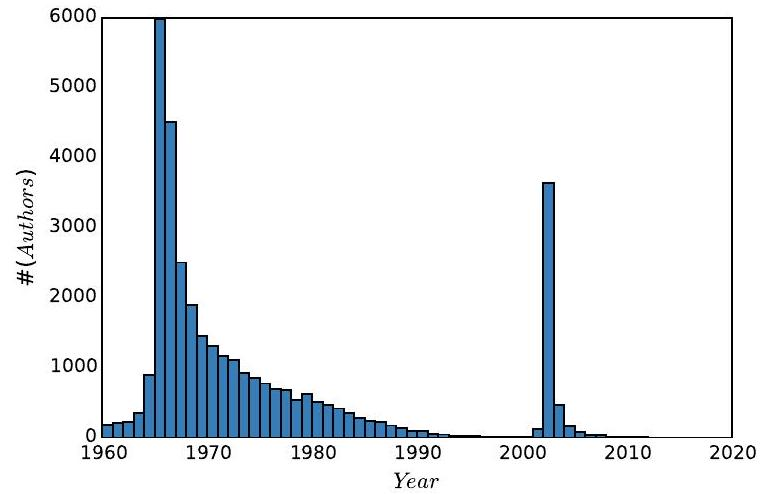
\includegraphics[max width=\textwidth]{2025_03_17_ca60ec0bfd96dcf8e028g-087}
    \caption{What artifacts can you find in this time series, counting the number of author's names first appearing in the scientific literature each year?}
    \label{fig:artifacts_time_series}
\end{figure}

प्रोसेसिंग कलाकृतियों का पता लगाने की कुंजी "स्निफ टेस्ट" है, उत्पाद को इतने करीब से देखना कि उसमें से कुछ खराब सूंघने को मिल सके। कुछ खराब आमतौर पर कुछ अप्रत्याशित या आश्चर्यजनक होता है क्योंकि लोग स्वाभाविक रूप से आशावादी होते हैं। आश्चर्यजनक अवलोकन वो हैं जिनके लिए डेटा वैज्ञानिक जीते हैं। वास्तव में, ऐसे अंतर्दृष्टियाँ मुख्य कारण हैं कि हम जो करते हैं, वह करते हैं। लेकिन मेरे अनुभव में, अधिकांश आश्चर्य कलाकृतियाँ ही होती हैं, इसलिए हमें उन्हें संदेह की दृष्टि से देखना चाहिए।

चित्र\ref{आकृति:अवशेष_समय_श्रृंखला}उज्जीवित परियोजना के एक परियोजना से संगणकीय परिणाम प्रस्तुत करता है जहाँ हमने वैज्ञानिक प्रकाशन की प्रक्रिया का अध्ययन किया। यह उन 100,000 सबसे उत्पादक लेखकों की समय श्रृंखला दर्शाता है, जिन्हें उनके पहले पेपर के Pubmed में आने के वर्ष के अनुसार वर्गीकृत किया गया है, जो बायोमेडिकल साहित्य का एक मूलतः पूर्ण ग्रंथ सूची है।

इस आकृति को ध्यान से अध्ययन करें, और देखें कि क्या आप कोई ऐसे तत्व खोज सकते हैं जो टिप्पणी करने योग्य हों। मुझे इनमें कम से कम दो दिखाई देते हैं। अगर आप यह पता लगा सकते हैं कि समस्या का कारण क्या था, तो अतिरिक्त श्रेय दिया जाएगा।

कला-वस्तुओं को खोजने की कुंजी डेटा में विसंगतियों की तलाश में है जो आपके अपेक्षाओं का विरोध करती हैं। \textit{कुंवारी लेखकों की संख्या के वितरण को} कैसा दिखना चाहिए, और समय के साथ यह कैसे बदलना चाहिए? पहले, जो आप देखना उम्मीद करते हैं उसका एक पूर्व वितरण बनाएं, ताकि आप तब संभावित विसंगतियों का उचित मूल्यांकन कर सकें।

मेरे अंतर्ज्ञान का कहना है कि नए शीर्ष वैज्ञानिकों का वितरण काफी समतल होना चाहिए क्योंकि हर उत्तराधिकारी स्नातक छात्र वर्ग के साथ नए सितारे जन्म लेते हैं। मैं यह भी अनुमान लगाऊंगा कि जनसंख्या के विस्तार के साथ धीरे-धीरे ऊपर की ओर प्रवाह हो सकता है, और अधिक लोग वैज्ञानिक समुदाय में प्रवेश करेंगे। लेकिन ऐसा मुझे आकृति \ref{fig:artifacts_time_series} में नहीं दिखता। तो कोशिश करें कि अनियमितताओं/संभावित कृत्रिमताओं को सूचीबद्ध करें...

\begin{figure}[h]
    \centering
    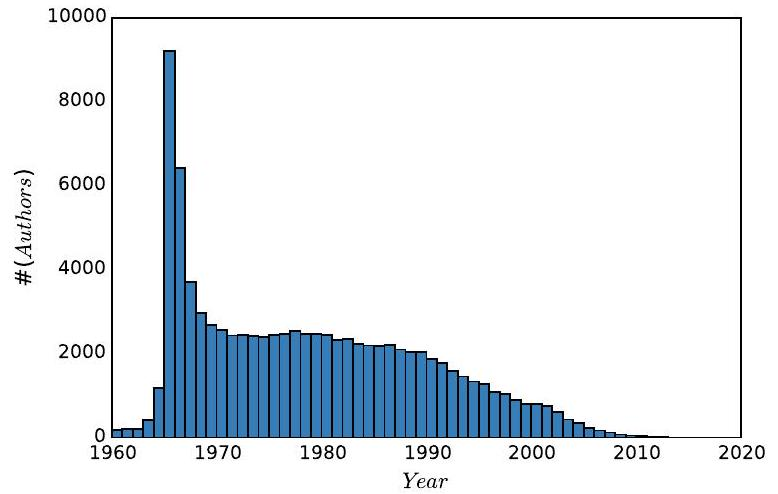
\includegraphics[max width=\textwidth]{2025_03_17_ca60ec0bfd96dcf8e028g-088}
    \caption{The cleaned data removes these artifacts, and the resulting distribution looks correct.}
    \label{fig:cleaned_data}
\end{figure}

जब मैं आरेख \ref{fig:artifacts_time_series} को देखता हूँ तो मुझे दो बड़े उभार दिखाई देते हैं: बायें उभार की शुरुआत लगभग 1965 के आसपास होती है, और एक चोटी जो 2002 में फूट पड़ती है। सोचने पर, बायाँ सबसे पहला उभार समझ में आता है। यह बायाँ चोटी उस वर्ष में आती है जब पबमेड ने पहली बार व्यवस्थित रूप से बिबलियोग्राफिक रिकॉर्ड्स को एकत्र करना शुरू किया था। हालांकि 1960-1964 से कुछ बहुत अधूरे डेटा हैं, उन पुराने वैज्ञानिकों का जो कई वर्षों से पेपर प्रकाशित कर रहे थे, "उभरना" 1965 में व्यवस्थित रिकॉर्ड्स की शुरुआत के साथ ही हुआ। तो यह बायाँ उभार समझाता है, जो फिर 1970 तक हल होता है और ऐसा दिखता है जैसा कि हमने सपाट वितरण की अपेक्षा की थी।

लेकिन वह विशाल 2002 शिखर के बारे में क्या? और उन वर्षों में नए लेखक लगभग शून्य तक क्यों गिर गए जो इसे पहले आते हैं? बड़े शिखर के दाईं ओर भी एक समान गिरावट दिखाई देती है। क्या दुनिया के सभी प्रमुख वैज्ञानिक 2002 में ही जन्म लेने वाले थे?

बड़े पीक में रिकॉर्ड की सावधानीपूर्वक जाँच ने विसंगति का स्रोत प्रकट किया: पहला नाम। पबमेड के शुरुआती दिनों में, लेखकों की पहचान उनके आद्याक्षर और अंतिम नामों द्वारा की जाती थी। लेकिन 2001 के अंत में,\textit{एसएस स्कीना}\textit{स्टीवेन एस. स्कीना}बन गए, तो यह\textit{ऐसा लगा}जैसे कोई नया लेखक आकाश से उभर रहा हो।

लेकिन इस शिखर के बाएँ और दाएँ शून्यता तक गिरावट क्यों होती है? याद रखें कि हमने इस अध्ययन को 100,000 सबसे उत्पादक वैज्ञानिकों तक सीमित रखा था। 1998 में उभरने वाला एक वैज्ञानिक रॉक स्टार इस रैंकिंग में आने की संभावना नहीं रखता क्योंकि उनका नाम कुछ वर्षों बाद बदलने के लिए बाध्य था, जिससे पूरे करियर के पत्रों को संचित करने के लिए पर्याप्त समय नहीं बचता। वितरण के बहुत दाएँ भी ऐसा ही होता है: 2010 में निर्मित नए वैज्ञानिक केवल कुछ वर्षों में पूरे करियर के काम को कभी हासिल नहीं कर पाएंगे। ये दोनों घटनाएँ इस पहले नाम के आधार पर अच्छी तरह समझाई जा सकती हैं।\index{p-values}\index{permutation!tests}

इस डेटा को साफ करके नाम सन्दर्भों को एकीकृत करने में हमें कुछ दोहरावों की आवश्यकता पड़ी। 2002 की चोटी को हटाने के बाद भी, हमने देखा कि 1990 के दशक के मध्य में प्रसिद्ध वैज्ञानिकों के करियर शुरू करने में काफी गिरावट आई थी। ऐसा इसलिये था क्योंकि कई लोगों के पास पहली नाम से पहले एक शानदार आधा करियर और पहली नाम के बाद दूसरा शानदार आधा करियर था, लेकिन वे एक महान पूर्ण करियर की सीमा तक नहीं पहुँच सके।

%---- Page End Break Here ---- Page : 71

किसी एकल अवधि में। इस प्रकार हमें शीर्ष 100,000 वैज्ञानिकों की पहचान करने से पहले पूरे\textit{पहले}सभी नामों को मेल करना था।

चित्र 3.3 हमारे अंतिम लेखक वितरण को दिखाता है, जो उस प्लैटोनिक आदर्श के साथ मेल खाता है जो हमें उम्मीद थी कि वितरण होगा। अपने डेटा को कंप्यूटर से निकलते हुए देखकर तुरंता तर्कसंगत बनाने के लिए बहुत जल्दी न करें। मेरे सहयोगी एक बार तो 2002 के उछाल को अनुसंधान फंडिंग में वृद्धि या नए वैज्ञानिक जर्नल्स के निर्माण के कारण खत्म मानने के लिए तैयार थे। हमेशा इस बात पर संदेह करें कि क्या आपका डेटा इतनी सफाई से तैयार है कि आप उस पर भरोसा कर सकें।

\subsection{डाटा अनुकूलता}
हम कहते हैं कि दो वस्तुओं की तुलना एक "सेब से सेब" की होती है जब यह एक न्यायोचित तुलना होती है, अर्थात् संबंधित वस्तुएँ इतनी समान होती हैं कि उन्हें समझदारी से एक दूसरे के खिलाफ खड़ा किया जा सकता है। इसके विपरीत, "सेब से संतरे" की तुलना अंततः अर्थहीन होती है। उदाहरण के लिए:

\begin{itemize}
  \item यह कोई समझदारी नहीं है कि 123.5 का वजन 78.9 से तुलना करें, जब एक पौंड में है और दूसरा किलोग्राम में।
  \item \textit{Gone with the Wind} की फिल्म कमाई की तुलना \textit{Avatar} से सीधे करना कोई समझदारी नहीं है, क्योंकि 1939 के डॉलर 2009 के डॉलर की तुलना में 15.43 गुना मूल्यवान हैं।
  \item आज न्यूयॉर्क और लंदन में दोपहर में सोने की कीमत की तुलना करना कोई समझदारी नहीं है, क्योंकि समय क्षेत्र पांच घंटे आगे-पीछे हैं, और उनके बीच में होने वाली घटनाओं से मूल्य प्रभावित होते हैं।
  \item 17 फरवरी, 2003 को माइक्रोसॉफ्ट के स्टॉक मूल्य की तुलना 18 फरवरी, 2003 से करना कोई समझदारी नहीं है, क्योंकि मध्यवर्ती 2-फॉर-1 स्टॉक विभाजन ने मूल्य को आधे में काट दिया, लेकिन वास्तविक मूल्य में कोई परिवर्तन नहीं दर्शाता।
\end{itemize}

जब भी डेटा सेट्स का मर्ज किया जाता है, तो इस प्रकार की डेटा तुलना समस्याएं उत्पन्न होती हैं। यहाँ मैं आपको यह दिखाने की आशा करता हूँ कि ऐसी तुलना समस्याएं कितनी घातक हो सकती हैं ताकि आपको इनके प्रति जागरूकता की जरूरत क्यों है, इसके प्रति संवेदनशील बनाया जा सके। इसके अलावा, कुछ महत्वपूर्ण वर्गों की रूपांतरण समस्याओं के लिए, मैं उन्हें संभालने के तरीकों की ओर इशारा करता हूँ।

\textit{घर पर सीखने का पाठ:} किसी भी आंकड़ा सेट के प्रत्येक क्षेत्र के अर्थ की समीक्षा करें जिसके साथ आप कार्य कर रहे हैं। यदि आप उसमें मापन इकाइयों तक क्या है यह नहीं समझते, तो इसका उपयोग करने का कोई समझदारी भरा तरीका नहीं हो सकता।

\section{इकाई परिवर्तन}
भौतिक प्रणालियों में अवलोकनों को मात्रा में बदलने के लिए मानक माप इकाइयों की आवश्यकता होती है। दुर्भाग्यवश, कई कार्यात्मक रूप से समान लेकिन असंगत मापन प्रणालियाँ मौजूद हैं। मेरी 12 वर्षीय बेटी और मेरा वजन लगभग 70 है, लेकिन हम में से एक का वजन पाउंड में और दूसरे का किलोग्राम में है।

विनाशकारी घटनाएँ जैसे रॉकेट विस्फोट तब होती हैं जब कंप्यूटर सिस्टम में माप गलत इकाइयों में दर्ज की जाती हैं। विशेष रूप से, नासा ने 23 सितंबर, 1999 को एक मीट्रिक-से-इंग्लिश परिवर्तन समस्या के कारण \$ 125 मिलियन मार्स क्लाइमेट ऑर्बिटर अंतरिक्ष मिशन को खो दिया।

ऐसी समस्याओं का सबसे अच्छा समाधान एकल मापन प्रणाली का चयन करके और उसी के प्रति ईमानदार रहकर किया जा सकता है। मेट्रिक प्रणाली पारंपरिक अंग्रेजी प्रणाली की तुलना में कई लाभ प्रदान करती है। विशेष रूप से, व्यक्तिगत मापों को स्वाभाविक रूप से एकल दशमलव मात्राओं के रूप में व्यक्त किया जाता है (जैसे 3.28 मीटर) अनपेक्षित मात्राओं के जोड़े (5 फीट, 8 इंच) के बजाय। यही समस्या कोण (रेडियन बनाम डिग्री/सेकंड) और वजन (किलोग्राम बनाम पाउंड/oz) मापते समय उत्पन्न होती है।\index{permutation!randomly generating}

मीट्रिक सिस्टम का पालन करने से अपने आप सभी तुलना संबंधी मुद्दे हल नहीं होते, क्योंकि ऐसा कुछ नहीं है जो आपको मीटर और सेंटीमीटर में ऊँचाईयों को मिलाने से रोक सके। लेकिन यह एक अच्छा आरंभ है।

आप अपने डेटा सेट्स को मर्ज करते समय असंगत इकाइयों के खिलाफ अपनी रक्षा कैसे कर सकते हैं? जागरूकता आपका मुख्य हथियार होना चाहिए। सुनिश्चित करें कि आपके डेटा सेट के प्रत्येक आंकिक स्तंभ के लिए अभिप्रेत इकाइयाँ आपको पता होनी चाहिए, और मर्ज करते समय संगतता की पुष्टि करें। कोई भी स्तंभ जिसके पास संबंधित इकाई या ऑब्जेक्ट प्रकार नहीं है, तुरंत संदिग्ध होना चाहिए।

जब विभिन्न स्रोतों से रिकॉर्ड को मर्ज किया जाता है, तो एक नया "उत्पत्ति" या "स्रोत" फ़ील्ड बनाना एक उत्कृष्ट प्रथā है जो यह पहचानने में मदद करता है कि प्रत्येक रिकॉर्ड कहां से आया है। कम से कम यह उम्मीद प्रदान करता है कि इकाई परिवर्तन की गलतियों को बाद में सुधारा जा सकता है, समस्याग्रस्त स्रोत के रिकॉर्ड पर प्रणालीगत रूप से कार्य करके।

आंशिक रूप से स्वचालित प्रक्रिया का उपयोग करके ऐसे समस्याओं का पता लगाया जा सकता है, जो सांख्यिकी महत्व परीक्षण से विकसित की जा सकती है, जिसकी चर्चा अनुभाग 5.3 में की जाएगी। मान लीजिए कि हम अंग्रेजी (फीट) और मीट्रिक (मीटर) मापों के संयुक्त डेटा सेट में मानव ऊंचाइयों की आवृत्तियों का प्लॉट करें। हम वितरण में 1.8 के आसपास एक शिखर और 5.5 के आसपास दूसरा शिखर देखेंगे। वितरण में एकाधिक शिखरों का अस्तित्व हमें संदिग्ध बना देना चाहिए। दो इनपुट जनसंख्याओं पर महत्व परीक्षण से उत्पन्न \textit{प}-मान हमारे संदेहों की पुष्टि की डिग्री की कठोर माप प्रदान करता है।

\section{साँख्यिकीय प्रदर्शनी रूपांतरण}
साँख्यिकीय विशेषताएँ गणितीय मॉडलों में शामिल करने के लिए सबसे आसान होती हैं। वास्तव में, कुछ मशीन लर्निंग एल्गोरिदम जैसे कि रैखिक प्रतिगमन और समर्थन वेक्टर मशीन केवल साँख्यिकीय-संकेतांकित डेटा के साथ काम करते हैं। लेकिन यहाँ तक कि संख्याओं को संख्याओं में बदलना भी एक सूक्ष्म समस्या हो सकता है। साँख्यिकीय क्षेत्र विभिन्न तरीकों से प्रदर्शित किए जा सकते हैं: पूरी संख्याओं के रूप में (123), दशमलव के रूप में (123.5), या यहाँ तक कि भिन्नों के रूप में (123 1/2)। संख्याओं को पाठ के रूप में भी प्रदर्शित किया जा सकता है, जिसमें "दस लाख" को 10000000 में कनवर्ट करना आवश्यक होता है साँख्यिकीय प्रसंस्करण के लिए।

संख्यात्मक प्रतिनिधित्व समस्याएं एक और रॉकेट जहाज को नष्ट करने के लिए श्रेय ले सकती हैं। एक एरियन 5 रॉकेट 4 जून, 1996 को \$500 मिलियन की लागत से प्रक्षेपित किया गया था, जो प्रस्थान के चालीस सेकेंड बाद ही विस्फोट हो गया, जिसका कारण अंततः एक 64-बिट फ़्लोटिंग पॉइंट संख्या को 16-बिट पूर्णांक में असफल परिवर्तन बताया गया।

पूर्णांक और फ्लोटिंग पॉइंट (वास्तविक) संख्याओं के बीच का अंतर बनाए रखना महत्वपूर्ण होता है। पूर्णांक गिनती की संख्याएँ होती हैं: मात्राएँ जो वास्तव में

%---- Page End Break Here ---- Page : 73

% Page : 73

वितरित को पूर्णांकों के रूप में प्रस्तुत किया जाना चाहिए। भौतिक रूप से मापी गई मात्राएँ कभी भी बिल्कुल मापी नहीं जातीं, क्योंकि हम एक निरंतर विश्व में रहते हैं। इसलिए सभी मापों को वास्तविक संख्याओं के रूप में रिपोर्ट किया जाना चाहिए। वास्तविक संख्याओं के पूर्णांक अनुमानों का कभी-कभी स्थान बचाने के लिए गलत प्रयास में उपयोग किया जाता है। ऐसा न करें: गोलाई या कटौती के मापन का प्रभाव कलाकृतियाँ उत्पन्न करता है।

एक विशेष रूप से गड़बड़ डेटा सेट में हमने पाया कि शिशु का वजन दो पूर्णांक क्षेत्रों (पाउंड और शेष औंस) के रूप में दर्शाया गया था। इसे एकल दशमलव मात्रा में संयोजित करना कहीं बेहतर होता।

\section{नाम एकीकरण}
दो भिन्न डेटा सेट्स से रिकॉर्ड्स को एकीकृत करने के लिए उन्हें किसी सामान्य कुंजी क्षेत्र को साझा करना आवश्यक होता है। नाम अक्सर कुंजी क्षेत्रों के रूप में उपयोग किए जाते हैं, लेकिन इन्हें अक्सर असंगत रूप से रिपोर्ट किया जाता है। क्या \textit{José} वही व्यक्ति है जो \textit{Jose} है? कई अमेरिकी राज्यों के आधिकारिक जन्म रिकॉर्ड्स से ऐसे डाइएक्रिटिक निशानों को प्रतिबंधित कर दिया गया है, उन्हें संगत बनाने के लिए एक आक्रामक कोशिश में।

एक अन्य उदाहरण के रूप में, डेटाबेस मेरी प्रकाशनाओं को मेरे पहले (\textit{Steve}, \textit{Steven}, या \textit{S.}), मध्य (\textit{Sol}, \textit{S.}, या खाली), और अंतिम (\textit{Skiena}) नाम के कार्टीज़ीयन उत्पाद के रूप में अर्थीकरण करते हैं, जो नौ विभिन्न परिवर्तनशीलताएं प्रदान करता है। और चीजें और भी खराब हो जाती हैं यदि हम गलत-स्पेलिंगों को शामिल करते हैं। मैं खुद को गूगल पर पहले नाम \textit{Stephen} और अंतिम नाम \textit{Skienna} और \textit{Skeina} के साथ ढूंढ़ सकता हूँ।

कुंजी द्वारा रिकॉर्ड्स को एकीकृत करना एक बहुत ही जटिल समस्या है, जिसका कोई जादुई समाधान नहीं है। यही कारण है कि आईडी नंबरों को आविष्कृत किया गया था, इसलिए यदि संभव हो तो उन्हें कुंजी के रूप में उपयोग करें।

सर्वोत्तम सामान्य तकनीक एकरूपता है: सरल पाठ रूपांतरण करके प्रत्येक नाम को एकल मानक संस्करण में परिवर्तित करना। सभी स्ट्रिंग्स को छोटे अक्षरों में परिवर्तित करने से (आमतौर पर सही) टकराव की संख्या बढ़ जाती है। मध्य नामों को समाप्त करना या कम से कम उन्हें संक्षेप में बदलने से और भी अधिक नाम मिलान/टकराव उत्पन्न होते हैं, जैसे पहले नामों को मानक संस्करण में मैप करना (जैसे सभी\textit{Steves}को\textit{Stevens}में बदलना)।

ऐसी किसी भी परिवर्तन की प्रक्रिया में फ्रेंकस्टाइन-लोगों के बनने का जोखिम होता है, जहाँ एकल रिकॉर्ड को कई शरीरों से जोड़ा जाता है। एप्प्लिकेशन्स में भिन्नता होती है कि अधिक खतरनाक स्थिति अधिक आक्रामकता के साथ जोड़ने में है या अत्यधिक सावधानी में। पता लगाएँ कि आपका कार्य इस स्पेक्ट्रम पर कहाँ स्थित है और उसके अनुसार कार्य करें।

डेटा सेट्स को मर्ज करने में एक महत्वपूर्ण चिंता का विषय है \textit{वर्णमाला कोड एकीकरण}। टेक्स्ट स्ट्रिंग्स में वर्णों को संख्यात्मक अभिव्यक्तियां सौंपी जाती हैं, जिसमें चिह्नों और अंकों के बीच की मैपिंग वर्णमाला कोड मानक द्वारा शासित होती है। दुर्भाग्यवश, सामान्य उपयोग में कई अलग-अलग वर्णमाला कोड मानक हैं, जिसका अर्थ है कि एक वेब पेज से जो आप स्क्रैप करते हैं, वह उसी वर्णमाला कोड में नहीं हो सकता जैसा कि उस प्रणाली द्वारा माना जाता है जो इसे प्रोसेस करेगी।

ऐतिहासिक रूप से, पुराने 7-बिट\textit{ASCII}कोड मानक को 8-बिट\textit{ISO 8859-1 Latin}अक्षरमाला कोड में विस्तारित किया गया, जिसमें कई यूरोपीय भाषाओं से वर्ण और विराम चिह्न जोड़े गए। \textit{UTF-8}सभी यूनिकोड वर्णों का एक एन्कोडिंग है, जो 8-बिट ब्लॉकों की परिवर्तनीय संख्या का उपयोग करता है, जो ASCII के साथ पीछे की संगत है। यह वेब-पृष्ठों के लिए प्रमुख एन्कोडिंग है, यद्यपि अन्य प्रणालियाँ अभी भी उपयोग में हैं।

% Page : 74

सही ढंग से चरित्र कोड को मर्ज करने के बाद एकीकृत करना लगभग असंभव है। आपके पास एक एकल कोड को मानक के रूप में चुनने का अनुशासन होना चाहिए, और प्रत्येक इनपुट फ़ाइल के एनकोडिंग की जाँच करनी चाहिए, उसे आगे के काम से पहले लक्ष्य में परिवर्तित करना चाहिए।

\section{समय/तिथि एकीकरण}
डेटा/समय स्टैम्प का उपयोग घटनाओं के सापेक्ष क्रम को समझने और घटनाओं को सापेक्ष एकसमानता द्वारा समूहित करने के लिए किया जाता है। कई स्रोतों से इवेंट डेटा को एकीकृत करने में सार्थक परिणाम सुनिश्चित करने के लिए सावधानीपूर्वक सफाई की आवश्यकता होती है।

पहले हम समय मापन में आने वाली समस्याओं पर विचार करें। दो कंप्यूटरों की घड़ियां कभी भी पूरी तरह से सहमत नहीं होतीं, इसलिए विभिन्न प्रणालियों से लॉग को ठीक से संरेखित करने के लिए मेहनत और अनुमान दोनों की आवश्यकता होती है। विभिन्न क्षेत्रों से डेटा के साथ काम करते समय समय क्षेत्र की समस्याएं भी होती हैं, साथ हीं दिन के उजाले की बचत समय में बदलाव से संबंधित स्थानीय नियमों में विविधताएं भी होती हैं।

सही उत्तर यहाँ सभी समय मापों को \textit{समन्वित सार्वभौमिक समय} (UTC) के साथ संरेखित करना है, जो पारंपरिक \textit{ग्रीनविच माध्य समय} (GMT) को शामिल करने वाला एक आधुनिक मानक है। एक संबंधित मानक है \textit{यूनिक्स समय},\index{UNIX time} जो गुरुवार, 1 जनवरी, 1970 को 00:00:00 UTC से बीते सेकंडों की संख्या के संदर्भ में किसी घटना का सटीक समय बताता है।

ग्रेगोरियन कैलेंडर प्रौद्योगिकी दुनिया में आम है, हालांकि विभिन्न देशों में कई अन्य कैलेंडर प्रणालियाँ उपयोग में हैं। कैलेंडर प्रणालियों के बीच परिवर्तन करने के लिए सूक्ष्म एल्गोरिद्म का उपयोग करना चाहिए, जैसा कि \cite{reingold2001calendrical} में वर्णित है। तारीख संरेखण के लिए एक बड़ी समस्या समय क्षेत्रों और अंतर्राष्ट्रीय तिथि रेखा की सही व्याख्या से संबंधित है।

समय शृंखला एकीकरण अक्सर व्यापार कैलेंडर की प्रकृति से जटिल हो जाता है। वित्तीय बाजार सप्ताहांत और छुट्टियों पर बंद रहते हैं, जिससे व्याख्या के प्रश्न उत्पन्न होते हैं जब आप, उदाहरण के लिए, शेयर की कीमतों को स्थानीय तापमान से सम्बंधित करते हैं। सप्ताहांत में तापमान मापने का सही समय क्या है, ताकि सप्ताह के अन्य दिनों के साथ संगति बनी रहे? पायथन जैसी भाषाओं में वित्तीय समय शृंखला डेटा के साथ इन मुद्दों को सही करने के लिए विस्तृत पुस्तकालय होते हैं। ऐसी ही समस्याएँ मासिक डेटा के साथ भी उत्पन्न होती हैं, क्योंकि महीने (और यहाँ तक कि वर्ष भी) अलग-अलग लंबाई के होते हैं।

\section{वित्तीय एकीकरण}
पैसा दुनिया को चलाता है, यही वजह है कि कई डेटा विज्ञान परियोजनाएँ वित्तीय समय श्रृंखलाओं के इर्द-गिर्द घूमती हैं। लेकिन पैसा गंदा हो सकता है, इसलिए इस डेटा को स्वच्छ करने की आवश्यकता होती है।

एक समस्या यहाँ पर है\textit{मुद्रा रूपांतरण},\index{currency conversion} जो एक मानकीकृत वित्तीय इकाई का उपयोग करके अंतरराष्ट्रीय मूल्य को दर्शाता है। मुद्रा विनिमय दरें किसी दिए गए दिन के भीतर कुछ प्रतिशत तक बदल सकती हैं, इसलिए कुछ अनुप्रयोगों को समय-संवेदनशील रूपांतरणों की आवश्यकता होती है। रूपांतरण दरें वास्तव में मानकीकृत नहीं होतीं। विभिन्न बाजारों में अलग-अलग दरें और\textit{स्प्रेड्स} होंगे, जो खरीदने और बेचने की कीमतों के बीच का अंतर होता है जो रूपांतरण की लागत को कवर करता है।

%---- Page End Break Here ---- Page : 75



अन्य महत्वपूर्ण सुधार मुद्रास्फीति के लिए है।\textit{पैसे का समय मूल्य}इसका अर्थ यह है कि आज का एक डॉलर (आमतौर पर) एक वर्ष बाद के एक डॉलर से अधिक मूल्यवान है, और ब्याज दरें भविष्य के डॉलर को छूट देने का सही तरीका प्रदान करती हैं। मुद्रास्फीति दरों का अनुमान वस्तुओं की टोकरी में मूल्य परिवर्तनों को ट्रैक करके लगाया जाता है, और समय के साथ डॉलर की क्रय शक्ति को मानकीकृत करने का एक तरीका प्रदान करती हैं।\index{data-driven}\index{exploratory data analysis}\index{hypothesis driven}\index{new data set}

समय के गैर-तुच्छ अवधियों में किसी मॉडल में बिना समायोजित कीमतों का उपयोग करना सिर्फ मुसीबत को न्योता देना है। मेरे विद्यार्थियों के एक समूह ने एक बार तीस साल की अवधि में शेयर की कीमतों और तेल की कीमतों के बीच देखी गई मजबूत संबंधता से बहुत उत्साहित हो गए और इस तरह उन्होंने एक कमोडिटी भविष्यवाणी मॉडल में शेयर की कीमतों का उपयोग करने का प्रयास किया। लेकिन दोनों वस्तुओं की कीमतें डॉलर में थी, बिना किसी समायोजन के जैसे कि वे मुद्रास्फीति में थी। मूलतः\textit{किसी}भी जोड़ी के वस्तुओं की कीमतों की समय श्रृंखला मुद्रास्फीति के लिए सही नहीं करने पर समय के साथ मजबूत संबंध बनाएगी।\index{summary statistics}

असल में, समय के साथ मूल्य परिवर्तनों को प्रस्तुत करने का सबसे सार्थक तरीका शायद अन्तर नहीं बल्कि \textit{प्रतिलाभ} है, जो प्रारंभिक मूल्य द्वारा उस अन्तर को सामान्यीकृत करता है।

\[
r_{i}=\frac{p_{i+1}-p_{i}}{p_{i}}
\]

यह अधिक एक प्रतिशत परिवर्तन के समान है, जिसमें यहाँ लाभ यह है कि इस अनुपात का लॉगरिदम लेना लाभ और हानि के लिए सममित हो जाता है।

वित्तीय समय श्रृंखलाओं में कई अन्य जटिलताएँ होती हैं जिन्हें साफ करने की आवश्यकता होती है। कई स्टॉक्स हर साल एक विशेष तिथि को\textit{डिविडेंड}का भुगतान शेयरधारकों को करते हैं। उदाहरण के लिए, माइक्रोसॉफ्ट 16 जनवरी को \$2.50 डिविडेंड का भुगतान करेगा। अगर उस दिन के व्यापार की शुरुआत में आपके पास माइक्रोसॉफ्ट का एक शेयर है, तो आपको यह चेक प्राप्त होगा, इसलिए डिविडेंड जारी होने के तुरंत बाद शेयर का मूल्य \$2.50 से गिर जाता है। यह मूल्य गिरावट शेयरधारक के लिए वास्तविक हानि को प्रतिबिंबित नहीं करती, लेकिन ठीक से साफ किए गए डेटा को स्टॉक की कीमत में डिविडेंड को शामिल करने की आवश्यकता होती है। यह कल्पना करना आसान है कि बिना सुधार के मूल्य डेटा पर प्रशिक्षित एक मॉडल डिविडेंड जारी होने से ठीक पहले शेयर बेचने की सीख ले रहा है, और इसे ऐसा करने के लिए अनुचित रूप से गर्व हो रहा है।

\subsection{लुप्त मानों से निपटना}

सभी डेटा सेट पूर्ण नहीं होते हैं। डेटा सफाई का एक महत्वपूर्ण पक्ष उन क्षेत्रों की पहचान करना है जिनके लिए डेटा उपलब्ध नहीं है, और फिर उनके लिए सही ढंग से पूर्ती करना:

\begin{itemize}
  \item एक जीवित व्यक्ति की मृत्यु का वर्ष क्या है?
  \item आपको उस सर्वेक्षण प्रश्न के साथ क्या करना चाहिए जिसे खाली छोड़ दिया गया है या उसमें एक स्पष्ट रूप से असंभव मान भर दिया गया है?
  \item उन घटनाओं की सापेक्षिक आवृत्ति क्या है जो एक सीमित आकार के नमूने में देखने के लिए बहुत दुर्लभ हैं?
\end{itemize}

संख्यात्मक डेटा सेट प्रत्येक मैट्रिक्स तत्व के लिए एक मान की अपेक्षा करते हैं। मिसिंग मान को शून्य पर सेट करना आकर्षक होता है, लेकिन सामान्यतः गलत होता है, क्योंकि हमेशा यह अस्पष्टता होती है कि क्या इन मानों की व्याख्या डेटा के रूप में की जानी चाहिए या नहीं।

क्या किसी का वेतन शून्य है क्योंकि वह बेरोज़गार है, या उसने सिर्फ़ सवाल का जवाब नहीं दिया?

बेतुके मानों का उपयोग नॉट-डाटा प्रतीकों के रूप में करने का खतरा यह है कि जब मॉडल बनाने का समय आता है, तो उन्हें डाटा के रूप में गलत तरीके से समझा जा सकता है। आयु, शिक्षा, और लिंग से वेतन का पूर्वानुमान करने के लिए प्रशिक्षित एक रेखीय प्रतिगमन मॉडल उन लोगों के साथ कठिनाई में होगा जिन्होंने प्रश्न का उत्तर देने से इनकार कर दिया।

$-1$ जैसे मान का उपयोग कोई डेटा नहीं प्रतीक के रूप में करने में शून्य जैसी ही कमियाँ होती हैं। वास्तव में, उस गणितज्ञ की तरह बनें जो ऋणात्मक संख्याओं से डरता है: उन्हें टालने के लिए कुछ न करें।

\textit{घर पर सीखने का पाठ}: दोनों कच्चे डाटा और इसकी साफ की गई प्रति को अलग-अलग बनाए रखें। कच्चा डाटा वास्तविक सत्य है, और इसे भविष्य के विश्लेषण के लिए पूर्ण रूप से संरक्षित करना महत्वपूर्ण है। साफ किया गया डाटा गायब मानों को भरने के लिए इंप्यूटेशन द्वारा सुधारा जा सकता है। लेकिन कच्चे डेटा को साफ किए गए डेटा से अलग रखें, ताकि हम अनुमान लगाने के लिए विभिन्न दृष्टिकोणों की जांच कर सकें।\index{Anscombe’s Quartet}\index{summary statistics}

तो हमें अनुपस्थित मानों से कैसे निपटना चाहिए? सबसे सरल दृष्टिकोण यह है कि सभी रिकॉर्ड हटा दिए जाएं जिनमें अनुपस्थित मान हों। जब तक यह पर्याप्त प्रशिक्षण डेटा छोड़ जाता है, तब तक यह तरीका ठीक काम करता है, बशर्ते अनुपस्थित मान गैर-प्रणाली संबंधी कारणों से अनुपस्थित हों। यदि जिन लोगों ने अपनी वेतन बताने से इनकार किया, वे सामान्य रूप से औसत से ऊपर होते हैं, तो इन रिकॉर्ड को हटाने से पूर्वाग्रहित परिणाम मिलेंगे।

लेकिन सामान्यतः हम कुछ अनुमानों के साथ रिकॉ़र्ड्स का उपयोग करना चाहते हैं जिनमें कुछ फील्ड्स गायब होती हैं। यह बेहतर हो सकता है कि गायब मूल्यों का अनुमान या \textit{प्रतिस्थापन} किया जाए, बजाय उन्हें खाली छोड़ने के। हमें गायब मूल्यों को भरने के लिए सामान्य विधियों की आवश्यकता होती है। उम्मीदवारों में शामिल हैं:

\begin{itemize}
  \item \textit{ह्युरिस्टिक-आधारित इम्प्यूटेशन}:\index{IMDb!heuristic-based} यदि अंतर्निहित डोमेन का पर्याप्त ज्ञान है, तो हमें कुछ क्षेत्रों के मूल्यों का यथोचित अनुमान लगाने में सक्षम होना चाहिए। अगर मुझे आपके मरने का वर्ष भरने की आवश्यकता है, तो \textit{जन्म वर्ष + 80} अनुमान लगाना औसतन सही साबित होगा, और अंतिम उत्तर की प्रतीक्षा करने की तुलना में बहुत तेज़ होगा।\index{exploratory data analysis!visualization}\index{visualization!tools}
  \item \textit{मीन वैल्यू इम्प्यूटेशन}: किसी वेरिएबल के औसत मान का उपयोग गायब मूल्यों के लिए प्रॉक्सी के रूप में करना आमतौर पर समझदारी भरा होता है। पहला, मीन के साथ अधिक मान जोड़ने से मीन अपरिवर्तित रहता है, इसलिए हम इस तरह की इम्प्यूटेशन द्वारा अपने सांख्यिकी में पक्षपात नहीं करते हैं। दूसरा, औसत मान वाले क्षेत्रों में अधिकांश मॉडलों में सादी स्वाद होती है, इसलिए उनके द्वारा डेटा का उपयोग करके बनाई गई किसी भी भविष्यवाणी पर उनका स्थिर प्रभाव होता है।
\end{itemize}

लेकिन अगर डेटा के गायब होने का कोई व्यवस्थित कारण हो, तो औसत उपयुक्त नहीं हो सकता है। मान लीजिए कि हमने विकिपीडिया में औसत मृत्य- वर्ष का इस्तेमाल करके सभी जीवित लोगों के लिए गायब मूल्य को पूरा करने की कोशिश की। यह विधि आपदा साबित होती, क्योंकि बहुत से लोगों के मरने का रिकॉर्ड उनके असल में जन्म लेने से पहले का होता।

\begin{itemize}
  \item \textit{रैंडम वैल्यू इम्प्यूटेशन}: एक और दृष्टिकोण यह है कि स्तंभ से एक रैंडम वैल्यू का चयन किया जाए ताकि अनुपलब्ध मान की जगह ली जा सके। यह तरीका संभवतः गलत अनुमान के लिए प्रेरित कर सकता है, लेकिन वास्तव में यही उद्देश्य है। बार-बार रैंडम वैल्यू का चयन करने से इम्प्यूटेशन के प्रभाव का सांख्यिकीय मूल्यांकन किया जा सकता है। अगर हम मॉडल को दस बार अलग-अलग इम्प्यूट किए गए
\end{itemize}

%---- Page End Break Here ---- Page : 77

% Mismatched: \sectionname{Dealing with Missing Values}

मूल्यों को प्राप्त करें और व्यापक रूप से भिन्न परिणाम प्राप्त करें, तो हमें संभवतः मॉडल पर अधिक विश्वास नहीं करना चाहिए। यह सटीकता जांच विशेष रूप से उपयोगी होती है जब डेटा सेट से मूल्यों का एक महत्वपूर्ण अंश गायब होता है।

\begin{itemize}
  \item \textit{निकटतम पड़ोसी द्वारा इम्पुटेशन}: क्या होगा अगर हम उस पूर्ण रिकॉर्ड की पहचान करें जो उपस्थित सभी क्षेत्रों पर सबसे निकटता से मेल खाता है, और इस निकटतम पड़ोसी का उपयोग यह अनुमान लगाने के लिए करें कि क्या गायब है? जब रिकॉर्ड्स के बीच भिन्नता को समझाने के लिए प्रणालीगत कारण होते हैं, तब इस तरह की भविष्यवाणियां औसत की तुलना में अधिक सटीक होनी चाहिए।
\end{itemize}

इस दृष्टिकोण के लिए एक दूरी फलन की आवश्यकता होती है ताकि सबसे समान अभिलेखों की पहचान की जा सके। \textit{सबसे निकट पड़ोसी} विधियाँ डेटा विज्ञान में एक महत्वपूर्ण तकनीक हैं, और उन्हें अधिक विस्तार से खंड 10.2 में प्रस्तुत किया जाएगा।

\begin{itemize}
  \item \textit{इम्पुटेशन बाई इंटरपोलेशन}: अधिक सामान्य रूप से, हम लक्षित स्तंभ के मानों की भविष्यवाणी करने के लिए एक विधि जैसे लीनियर रिग्रेशन (अनुभाग 9.1 देखें) का उपयोग कर सकते हैं, जब रिकॉर्ड में अन्य फ़ील्ड दिए गए हों। इस प्रकार के मॉडल पूरे रिकॉर्ड्स पर प्रशिक्षित किए जा सकते हैं और फिर उन्हें उन रिकॉर्ड्स पर लागू किया जा सकता है जिनमें मान गायब हैं।\index{Tufte, Edward}\index{visualization aesthetic}\index{visualization aesthetic!chartjunk}\index{visualization aesthetic!data-ink ratio}\index{visualization aesthetic!lie factor}\index{visualization aesthetic!scaling and labeling}
\end{itemize}

लाइनियर रिग्रेशन का उपयोग करके गायब मानों की भविष्यवाणी करना तब सबसे अच्छा होता है जब प्रति रिकॉर्ड केवल एक ही फील्ड गायब हो। यहाँ संभावित खतरा खराब भविष्यवाणियों के माध्यम से महत्वपूर्ण आउट्लायर्स बनाना है। रिग्रेशन मॉडल आसानी से अधूरे रिकॉर्ड को आउट्लायर बना सकते हैं, यानि गायब फील्ड्स में असामान्य रूप से ऊँचे या निम्न मान भर कर। इससे निम्न स्तरीय विश्लेषण का ध्यान उन रिकॉर्ड्स पर अधिक केंद्रित हो जाएगा जिनमें मान गायब हैं, जो बिलकुल वह नहीं है जो हम करना चाहते हैं।

ऐसी चिंताएं आउट्लायर डेटेक्शन के महत्व को उजागर करती हैं, जो सफाई प्रक्रिया का अंतिम कदम है जिसे यहाँ पर विचार किया जाएगा।

\subsection{अपवर्जक पहचान}

डेटा संग्रह में गलतियाँ आसानी से बाहरी मूल्यों का उत्पादन कर सकती हैं जो उचित विश्लेषण में बाधा डाल सकती हैं। एक दिलचस्प उदाहरण अब तक खोजी गई सबसे बड़ी डायनासोर कशेरुका से संबंधित है। 1500 मिलीमीटर में मापी गई, यह दर्शाता है कि वह व्यक्ति 188 फीट लंबा था। यह अद्भुत है, खासकर क्योंकि \textit{दूसरा} सबसे बड़ा नमूना अब तक केवल 122 फीट लंबा पाया गया है।

यहाँ सबसे संभावित स्पष्टीकरण (देखें \cite{goldenberg2016biggest}) यह है कि यह विशाल जीवाश्म वास्तव में कभी अस्तित्व में नहीं था: यह एक सौ वर्षों से अधिक समय से अमेरिकन म्यूजियम ऑफ नैचुरल हिस्ट्री से गायब रहा है। शायद मूल माप एक पारंपरिक आकार की हड्डी पर लिया गया था और बीच के दो अंकों को गलती से बदल दिया गया, जिससे कशेरुका 1050 मिलीमीटर तक घट गई।

आकस्मिक तत्व अक्सर डेटा प्रविष्टि में गलतियों से उत्पन्न होते हैं, जैसा कि यहाँ हुआ प्रतीत होता है। ये स्क्रैपिंग में त्रुटियों के कारण भी हो सकते हैं, जैसे कि प्रारूपण में अनियमितता के कारण फुटनोट संख्या को संख्यात्मक मूल्य के रूप में व्याख्यायित किया जाना। सिर्फ इसलिए कि कुछ लिखा गया है, इसका मतलब यह नहीं कि यह सही है। डायनासोर उदाहरण की तरह, एक अकेला आकस्मिक तत्व बड़ी भ्रांतियों को जन्म दे सकता है।

सामान्य तर्कसंगतता जाँच में प्रत्येक चर/कॉलम में सबसे बड़े और सबसे छोटे मानों को देखना शामिल होता है ताकि यह देखा जा सके कि वे कहीं असामान्य तो नहीं हैं। इसे सबसे अच्छे तरीके से फ़्रीक्वेन्सी हिस्टोग्राम को प्लॉट करके और चरम तत्वों की स्थिति को देखकर किया जा सकता है। दृश्य निरीक्षण भी पुष्टि कर सकता है कि वितरण उसी प्रकार का दिखता है जैसा कि इसे होना चाहिए, आमतौर पर घंटी के आकार का।

सामान्यरूप से वितरण किए गए डेटा में, किसी मान के माध्य से $k$ मानक विचलन दूर होने की प्रायिकता $k$ के साथ सूक्ष्म रूप से घटती है। यह स्पष्ट करता है कि 10 फुट लंबे बास्केटबॉल खिलाड़ी क्यों नहीं होते हैं, और यह बाहरी मान पहचाने के लिए एक ठोस सीमा प्रदान करता है। पॉवर लॉ वितरणों में बाहरी मान पहचानना इतना सरल नहीं होता है: वास्तव में \textit{ऐसा} एक बिल गेट्स होता है जो औसत व्यक्ति की तुलना में 10,000 गुना से अधिक मूल्य का होता है।\index{lie factor}\index{visualization aesthetic!lie factor}

सिर्फ आउट्लायर फ़ील्ड वाली पंक्तियों को हटाकर आगे बढ़ जाना बहुत सरल है। आउट्लायर्स अक्सर और अधिक प्रणालीगत समस्याओं की ओर इशारा करते हैं जिन्हें किसी को संभालना चाहिए। जीवनकाल के हिसाब से ऐतिहासिक आंकड़ों के एक सेट पर विचार करें। बाइबिल के मेथुसलह (969 वर्ष की आयु में) को आउट्लायर के रूप में चिह्नित करना और उन्हें हटा देना आसान है।

लेकिन यह समझना बेहतर है कि क्या वह अन्य आंकड़ों का संकेत देता है जिन्हें हमें हटाने पर विचार करना चाहिए। ध्यान दें कि मेथ्यूसेलाह की कोई निश्चित रूप से स्थापित जन्म और मृत्यु की तिथियाँ नहीं थीं। शायद किसी भी व्यक्ति की प्रकाशित आयु जिनकी तिथियाँ नहीं हैं, उसे काटने के लिए पर्याप्त संदिग्ध माना जाना चाहिए। इसके विपरीत, विकिपीडिया में सबसे कम जीवनकाल वाला व्यक्ति (फ्रांस के राजा जॉन I) केवल पाँच दिन जीवित रहा। लेकिन सन 1316 में उसकी जन्म (नवंबर 15) और मृत्यु (नवंबर 20) की तिथियाँ मुझे आश्वस्त करती हैं कि उसके जीवनकाल का विवरण सही था।

\section{युद्ध कथा: बीटिंग द मार्केट}

हर बार जब हम मिले, तो मेरा स्नातक छात्र वेनबिन मुझे बताता था कि हम पैसा कमा रहे हैं। लेकिन जब भी मैंने पूछा, उसकी आवाज में आत्मविश्वास कम होता गया।

हमारे लिडिया सेंटिमेंट विश्लेषण प्रणाली ने समाचार और सोशल मीडिया के विशाल टेक्स्ट फीड को लिया, जिससे लाखों विभिन्न लोग, स्थान, और संगठनों के लिए दैनिक समय श्रृंखला में उनका सेंटिमेंट और आवृत्ति कम किया जा सके। जब कोई व्यक्ति खेल चैंपियनशिप जीतता है, तो कई लेख लिखे जाते हैं जो बताते हैं कि वे कितने महान एथलीट हैं। लेकिन जब यह खिलाड़ी फिर ड्रग के आरोप में फंस जाता है, तो उनके बारे में लेखों का स्वर तुरंत बदल जाता है। सकारात्मक शब्दों (``विजयी'') और नकारात्मक शब्दों (``गिरफ्तार'') के साथ संबद्धता की सापेक्ष आवृत्ति की गिनती करके, हम किसी भी समाचार योग्य इकाई के लिए सेंटिमेंट संकेत उत्पन्न कर सकते हैं।

वेनबिन ने अध्ययन किया कि भावना संकेतों का उपयोग भविष्य की घटनाओं जैसे कि किसी दिए गए फिल्म की सकल आय की भविष्यवाणी करने के लिए कैसे किया जा सकता है, प्रकाशित समीक्षाओं या खबरों की गुणवत्ता के आधार पर। लेकिन वह विशेष रूप से इस डेटा का उपयोग स्टॉक बाजार में खेल खेलने के लिए करना चाहते थे।\index{stock market} स्टॉक समाचार के अनुसार ऊपर और नीचे जाते हैं। आय रिपोर्ट का छूट जाना किसी कंपनी के लिए बुरी खबर है, इसलिए कीमत नीचे जाती है। खाद्य और औषधि प्रशासन (एफडीए) द्वारा किसी नए दवा की स्वीकृति उस कंपनी के लिए\textit{महान}खबर है जो इसे मालिक है, इसलिए कीमत ऊपर जाती है। अगर वेनबिन हमारे भावना संकेत का उपयोग करके भविष्य के स्टॉक मूल्य की भविष्यवाणी कर सकते थे, तो चलो बस यह कहें कि मुझे अब उन्हें रिसर्च असिस्टेंट के रूप में भुगतान नहीं करना पड़ता।

तो उसने उन स्टॉक्स को खरीदने की रणनीति का अनुकरण किया जो सबसे अधिक

%---- Page End Break Here ---- Page : 79

\section{जनस्रोतः प्रणाली}
\index{crowdsourcing}\label{अनुभाग:जनस्रोतः}

कोई भी व्यक्ति सभी उत्तर नहीं जानता। यहाँ तक कि मैं भी नहीं। जो ज्ञान के रूप में हमें प्रतीत होता है, वह वास्तव में विशेषज्ञता का संयोजन होता है, जो दूसरों के ज्ञान और अनुभव से मतों का संग्रहण होता है।

\begin{figure}[h!]
\centering
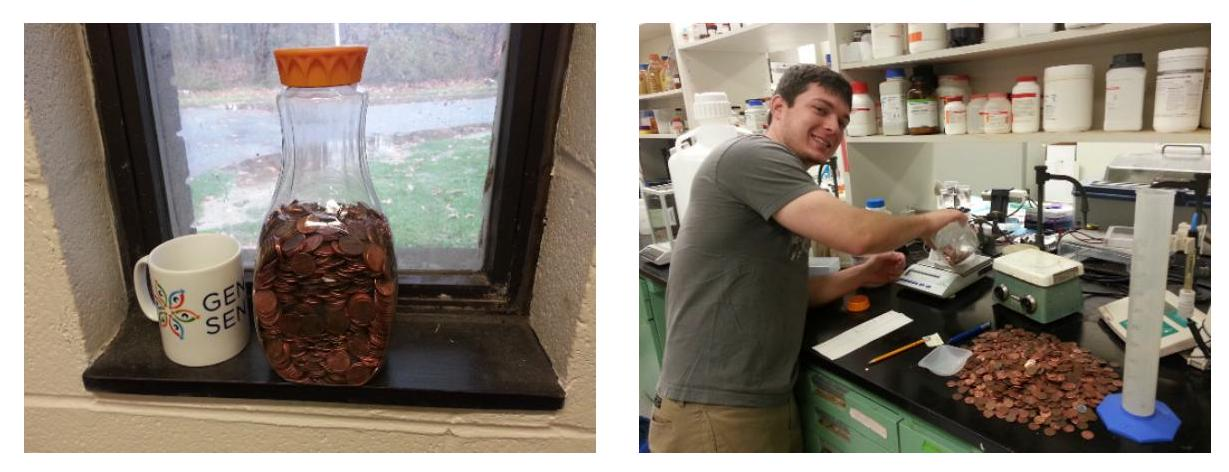
\includegraphics[max width=\textwidth]{2025_03_17_ca60ec0bfd96dcf8e028g-098}
\caption{Guess how many pennies I have in this jar? (left) The correct answer was determined using precise scientific methods (right).}
\label{fig:penny_jar}
\end{figure}

क्राउडसोर्सिंग बड़ी संख्या में लोगों की अंतर्दृष्टि और श्रम को एक सामान्य लक्ष्य की ओर उपयोग करती है। यह \textit{भीड़ की समझदारी} का लाभ उठाती है,\index{wisdom of crowds} कि एक समूह के लोगों का सामूहिक ज्ञान शायद उनकी सबसे चतुर व्यक्ति की तुलना में अधिक हो सकता है।

यह धारणा बैल से शुरू हुई। फ्रांसिस गैल्टन, जो सांख्यिकी विज्ञान के संस्थापक और चार्ल्स डार्विन के रिश्तेदार थे, ने 1906 में एक स्थानीय पशु मेले में भाग लिया। उत्सव के एक हिस्से के रूप में, गाँववासियों को इस विशेष बैल का वजन अनुमानित करने के लिए आमंत्रित किया गया था, जिसमें जिस व्यक्ति का अनुमान सटीक के करीब होता उसे पुरस्कार मिलता। लगभग 800 प्रतिभागियों ने इसमें हिस्सा लिया। किसी ने भी वास्तविक वजन 1,178 पाउंड नहीं चुना, फिर भी गैल्टन ने देखा कि औसत अनुमान आश्चर्यजनक रूप से करीब था: 1,179 पाउंड! गैल्टन के प्रयोग से यह सुझाव निकलता है कि कुछ कार्यों के लिए केवल विशेषज्ञों से पूछने के बजाय विभिन्न लोगों के समूह को शामिल करके बेहतर परिणाम प्राप्त किए जा सकते हैं।

भीड़सोर्सिंग मॉडल बनाने में डेटा का एक महत्वपूर्ण स्रोत होती है, विशेष रूप से उन कार्यों के लिए जो मानव धारणा से जुड़े होते हैं। प्राकृतिक भाषा प्रसंस्करण और कंप्यूटर विज़न में मनुष्य राज्य-के-आर्ट सिस्टम बने रहते हैं, और उच्चतम प्रदर्शन स्तर प्राप्त करते हैं। प्रशिक्षण डेटा एकत्र करने का सबसे अच्छा तरीका अक्सर लोगों से एक विशेष पाठ या छवि को स्कोर करने के लिए कहना होता है। इसे पर्याप्त पैमाने पर करने के लिए पर्याप्त प्रशिक्षण डेटा बनाने के लिए आमतौर पर बड़ी संख्या में टिप्पणीकारों की आवश्यकता होती है, वास्तव में एक भीड़ की।

सोशल मीडिया और अन्य नई तकनीकों ने बड़े पैमाने पर विचारों को इकट्ठा करना और संकलित करना आसान बना दिया है। लेकिन हम भीड़ की समझदारी को भीड़ की चिल्लाहट से कैसे अलग करें?

\subsection{पैनी डेमो}
\label{उपधारा:पैनी_डेमो}

चलो अपनी खुद की भीड़ की बुद्धिमत्ता प्रयोग करके शुरू करते हैं। आकृति\ref{आकृति:पैनी_जार}में मेरे कार्यालय में कई वर्षों के दौरान जमा किए गए पैनी का एक जार की तस्वीरें हैं। इस जार में मेरे पास कितने पैनी हैं? अब अपनी स्वयं की अनुमान लगाएं, क्योंकि मैं आपको अगला पृष्ठ पर उत्तर बताने जा रहा हूं।\index{visualization aesthetic!colors}\index{visualization aesthetic!repetition}

%---- Page End Break Here ---- Page : 81

सही उत्तर प्राप्त करने के लिए, मैंने जैवविज्ञानी-सहयोगी जस्टिन गार्डन से पेंसियों का वजन एक सटीक प्रयोगशाला तराजू पर तौलने के लिए कहा। एक पेंस के वजन से विभाजित करने पर संख्या मिलती है। जस्टिन को लगन से अपना कार्य करते हुए चित्र 3.4 (दाहिने) में देखा जा सकता है।

तो मैं फिर से पूछता हूँ: तुम्हें क्या लगता है, इस जार में मेरे पास कितने पेनीज़ हैं? मैंने यह प्रयोग अपने डेटा साइंस क्लास के छात्रों पर किया। तुम्हारा जवाब उनके जवाबों से कैसे तुलना करेगा?

मैंने पहले अपने ग्यारह छात्रों से कहा कि वे अपने विचार कार्डों पर लिखें और कमरे के सामने चुपचाप मुझे सौंप दें। इस प्रकार ये अनुमान पूरी तरह से एक दूसरे से स्वतंत्र थे। सुविधा के लिए व्यवस्थित परिणाम इस प्रकार थे:

\[
537, 556, 600, 636, 1200, 1250, 2350, 3000, 5000, 11,000, 15,000.
\]

मैंने फिर इन संख्याओं को बोर्ड पर लिखा और कुछ सांख्यिकी का गणना किया। इन अनुमानों का माध्यिका 1250 था, और औसत 3739 था। वास्तव में, जार में कुल 1879 पेनियाँ थीं। मेरे छात्रों के बीच माध्यिका स्कोर सही मात्रा के सबसे नज़दीक था, बजाय किसी एकल अनुमान के।

लेकिन वास्तविक कुल प्रकट करने से पहले, मैंने फिर दर्जन भर और छात्रों से अनुमान लगाने के लिए कहा। केवल एक अंतर यह था कि इस समूह ने बोर्ड पर लिखे पहले समूह के छात्रों के अनुमान देखे थे। उनके चुनाव थे: 
\[
750, 750, 1000, 1000, 1000, 1250, 1400, 1770, 1800, 3500, 4000, 5000। 
\]
अन्य लोगों के अनुमानों को इस समूह के सामने उजागर करने से वितरण को मजबूत ढंग से प्रभावित किया गया और सभी बाहरी अनुमान समाप्त हो गए: दूसरे समूह में न्यूनतम, पहले के चार अनुमानों से अधिक था, और अधिकतम, पिछले दौर के तीन अनुमानों के बराबर या कम था। इस समूह में, मध्यिका 1325 थी और औसत 1935। दोनों ही वास्तविक उत्तर के कुछ करीब थे, लेकिन यह स्पष्ट है कि समूह की सोच ने इसे संभव बनाने के लिए अपने पैर पसार लिए थे।

\textit{एंकरिंग} एक प्रसिद्ध संज्ञानात्मक पक्षपात है जिसमें लोगों के निर्णय अनौचित्यपूर्ण रूप से उस पहले संख्या पर स्थिर हो जाते हैं जो वे सुनते हैं। कार डीलर इसको हमेशा उपयोग में लेते हैं, पहले वाहन की एक ऊँची कीमत देकर ताकि बाद की कीमतें एक सस्ते सौदे की तरह सुनाई दें।

मैंने उत्तर को प्रकाशित करने से पहले एक अंतिम परीक्षण किया। मैंने अपने छात्रों को बोली लगाने की अनुमति दी, जिसका मतलब था कि उन्हें परिणाम पर पैसे लगाने के लिए पर्याप्त आत्मविश्वासी होना पड़ा। इसने दो साहसी छात्रों से क्रमशः 1500 और 2000 पेनियों की बोली प्राप्त हुई। मैंने उच्च बोली लगाने वाले से $1.21 अपनी जेब में रखे, लेकिन दोनों बोली काफी करीब साबित हुई। यह कोई आश्चर्य की बात नहीं है: जो लोग किसी घटना पर अपने पैसे लगाने को तैयार होते हैं, वे परिभाषा के अनुसार अपनी पसंद को लेकर आत्मविश्वासी होते हैं।

\subsection{भीड़ कब बुद्धिमान होती है?}
जेम्स सुरोविकी के अनुसार अपनी पुस्तक\textit{द विज़डम ऑफ क्राउड्स}\cite{surowiecki2005wisdom} में, भीड़ तब बुद्धिमान होती है जब चार शर्तें पूरी होती हैं:

\begin{itemize}
\item \textit{जब राय स्वतंत्र होती हैं:} हमारा प्रयोग यह उजागर करता है कि एक समूह कितनी आसानी से समूह विचारधारा में फंस सकता है। लोग स्वाभाविक रूप से दूसरों से प्रभावित होते हैं। यदि आप किसी की सच्ची राय चाहते हैं, तो आपको उन्हें अकेले में पूछना चाहिए।
\item \textit{जब भीड़ में विविध ज्ञान और विधियों वाले लोग होते हैं:} विवाद होने पर ही भीड़ सूचना जोड़ती है। पूर्णत: संबंधित विशेषज्ञों से बना एक समिति कुछ नहीं जोड़ता है जो आप उनमें से किसी एक से जान सकते थे। पेनिंग अनुमान समस्या में, कुछ लोग कंटेनर की आयतन का अनुमान लगाते थे, जबकि अन्य मेरी बांह के झुकने का अंदाजा लगाते थे जब मैंने भारी बोझ उठाया। वैकल्पिक दृष्टिकोण यह अनुमान लगा सकते थे कि बीस वर्षों में मेरी जेब से कभी-कभी खाली होने पर मैं कितनी पेनियां जमा कर सकता था, या अपनी खुद की संग्रह की अनुभवों को याद कर सकते थे।
\item \textit{जब समस्या का क्षेत्र ऐसा हो जिसमें विशेष ज्ञान की जरूरत न हो:} मैं कुछ महत्वपूर्ण निर्णयों में भीड़ की सहमति पर विश्वास करता हूँ, जैसे कौन सी कार खरीदनी चाहिए या मेरे देश का राष्ट्रपति कौन होना चाहिए (गुल्प)। लेकिन जब यह तय करने की बात आती है कि मेरी ट्यूमर का नमूना कैंसरयुक्त है या सौम्य, मैं एक डॉक्टर के वचन पर भरोसा करूंगा बजाय 1,000 नामों के यादृच्छिक रूप से फोन बुक से लिए गए लोगों की भीड़ के। क्यों? क्योंकि यहां सवाल विशेष ज्ञान और अनुभव से अत्यधिक लाभान्वित होता है। डॉक्टर को वास्तव में सभी अन्य से अधिक पता होने का एक वास्तविक कारण होता है। सरल धारणा कार्यों के लिए भीड़ का शासन होता है, लेकिन आपको भीड़ से कुछ ऐसा पूछने से बचना चाहिए जो उन्हें नहीं पता।
\item \textit{रायों को सही ढंग से संकलित किया जा सकता है:} किसी भी जन सर्वेक्षण फॉर्म का सबसे कम उपयोगी भाग खुला प्रतिक्रिया क्षेत्र "हमें बताएं कि आप क्या सोचते हैं!" होता है। समस्या यहां यह है कि इन रायों को एक सहमति में मिलाने का कोई तरीका नहीं है, क्योंकि अलग-अलग लोगों की अलग-अलग समस्याएं और चिंताएं होती हैं। शायद इन टेक्स्ट्स को समानता के अनुसार बाल्टी में डाला जा सकता है, लेकिन इसे प्रभावी ढंग से करना कठिन होता है। इस तरह की स्वतंत्र-प्रारूप प्रतिक्रियाओं का सबसे सामान्य उपयोग उपाख्यानात्मक होता है। लोग सबसे सकारात्मक-साउंडिंग को चुनते हैं, फिर उन्हें एक स्लाइड पर डालते हैं ताकि बॉस को प्रभावित कर सकें।
}

\textit{घर ले जाने का पाठ:} जीवन की आंशिक क्रम में एक अपूर्व तत्व बनें। विविध, स्वतंत्र सोच भीड़ में सबसे अधिक ज्ञान का योगदान देती है।

\subsection{संग्रहण के लिए तंत्र}
प्रतिक्रियाओं के एक सेट से ज्ञान एकत्रित करने के लिए सही संग्रहण तंत्र का उपयोग करना आवश्यक होता है। संख्यात्मक मात्राओं का अनुमान लगाने के लिए, आवृत्ति वितरण का चित्रण करना और संक्षिप्त सांख्यिकी गणना करना मानक तकनीकें होती हैं। औसत और माध्य दोनों ही त्रुटियों को अप्रत्यक्ष रूप से मानते हैं कि वे

%---- Page End Break Here ---- Page : 83

माध्यिका, सामान्य रूप से, ऐसे संकलन समस्याओं में माध्य के मुकाबले अधिक उपयुक्त विकल्प होती है। यह अपवादात्मक मानों के प्रभाव को कम करता है, जो बड़े प्रयोगों के मामले में एक विशेष समस्या होती है, जहाँ आपके प्रतिभागियों का एक निश्चित हिस्सा अपेक्षित रूप से विफल हो सकता है। हमारे पैसा अनुमान डेटा पर, माध्य ने 3739 का भयानक अधिक-आकलन उत्पन्न किया, जो सबसे बड़ा और सबसे छोटा अनुमान हटाने के बाद 2843 तक घट गया, और फिर प्रत्येक छोर पर दो अपवादात्मक मानों को छाँटने के बाद 2005 तक कम हो गया (सही उत्तर 1879 था)।\index{box plots}\index{line charts!best practices}\index{uncertainty}\index{chart types!dot and line plots}\index{line charts}\index{line charts!advantages}

आउटलाइअर हटाना एक बहुत अच्छी रणनीति है, लेकिन हमारे विषयों की विश्वसनीयता का मूल्यांकन करने के लिए हमारे पास अन्य आधार भी हो सकते हैं, जैसे कि अन्य परीक्षणों पर उनका प्रदर्शन जहां हमें उत्तर ज्ञात हैं। \textit{वेटेड एवरेज} लेना, जिसमें हम उन अंकों को अधिक महत्व देते हैं जिन्हें अधिक विश्वसनीय माना जाता है, ऐसे आत्मविश्वास उपायों को ध्यान में रखने का एक तरीका प्रदान करता है।

वर्गीकरण समस्याओं के लिए, मतदान मूलभूत संचयन तंत्र है। \textit{कोंडोर्सेट ज्यूरी प्रमेय}प्रजातंत्र में हमारे विश्वास को उचित ठहराता है। यह कहता है कि यदि प्रत्येक मतदाता के सही होने की संभावना किसी दिए गए मुद्दे पर$p > 0.5$ है, तो बहुमत मतदाताओं के सही होने की संभावना\(P(n)\)प से अधिक है। वास्तव में, यह बिलकुल यह है:

\[
P(n)=\sum_{i=(n+1) / 2}^{n}\binom{n}{i} p^{i}(1-p)^{n-i}
\]

बड़े मतदाता गिनती आँकड़ों की प्रामाणिकता देती हैं, यहाँ तक कि अधिक विवादस्पद चुनावों में भी। मान लीजिए\(p=0.51\), जिसका अर्थ है कि सही ताकतें एक मामूली बहुमत हैं। 101 सदस्यों की एक जूरी सही निर्णय 57\% समय पर पहुँचती है, जबकि\(P(1001)=0.73\)और\(P(10001)=0.9999\)। एक सही निर्णय की संभावना 1 के करीब होती है जैसे-जैसे\(n\rightarrow\infty\)।

चुनावी प्रणालियों की शक्ति की प्राकृतिक सीमाएँ होती हैं, हालांकि। \textit{एरो का असंभवता प्रमेय} बताता है कि प्राथमिकताओं की क्रम अनुक्रमणिका को वोट्स के रूप में जोड़ने के लिए कोई चुनावी प्रणाली ऐसा नहीं करती जो चुनाव की निष्पक्षता के लिए चार प्राकृतिक शर्तों को पूरा करती हो। इसे सेक्शन 4.6 में स्कोर और रैंकिंग के संदर्भ में चर्चा की जाएगी।

% Mismatched: \sectionname{Crowdsourcing Services}

क्राउडसोर्सिंग सेवाएं जैसे ऐमज़ॉन टर्क और क्राउडफ्लावर आपको एक बड़े समूह के लोगों को छोटे-छोटे काम करने के लिए किराए पर लेने का अवसर प्रदान करती हैं। ये सेवाएं आपको लोगों को प्रबंधित करने में मदद करती हैं, ताकि आप अपने लिए डेटा बनाने के लिए उन्हें व्यवस्थित कर सकें।

ये भीड़-स्रोत सेवाएं फ्रीलांस श्रमिकों का एक बड़ा स्थिर बनाए रखते हैं, जो उनके और संभावित नियोक्ताओं के बीच मध्यस्थ के रूप में काम करते हैं। इन श्रमिकों को आमतौर पर \textit{टर्कर्स} कहा जाता है, जिन्हें उपलब्ध नौकरियों की सूची और उनकी भुगतान राशि प्रदान की जाती है, जैसा कि चित्र 3.5 में दिखाया गया है। नियोक्ताओं के पास आम तौर पर यह नियंत्रित करने की कुछ क्षमता होती है कि वे किस स्थान और योग्यताओं वाले व्यक्ति को काम पर रख रहे हैं, और यदि वे कार्य को अपर्याप्त मानते हैं तो बिना भुगतान के श्रमिक की कोशिशों को अस्वीकार करने की शक्ति भी रखते हैं। लेकिन नियोक्ताओं की स्वीकृति दरों पर आँकड़े प्रकाशित किए जाते हैं, और अच्छे श्रमिक खराब गुण वाले लोगों के लिए काम करने की संभावना नहीं रखते हैं।

\begin{figure}[h]
    \centering
    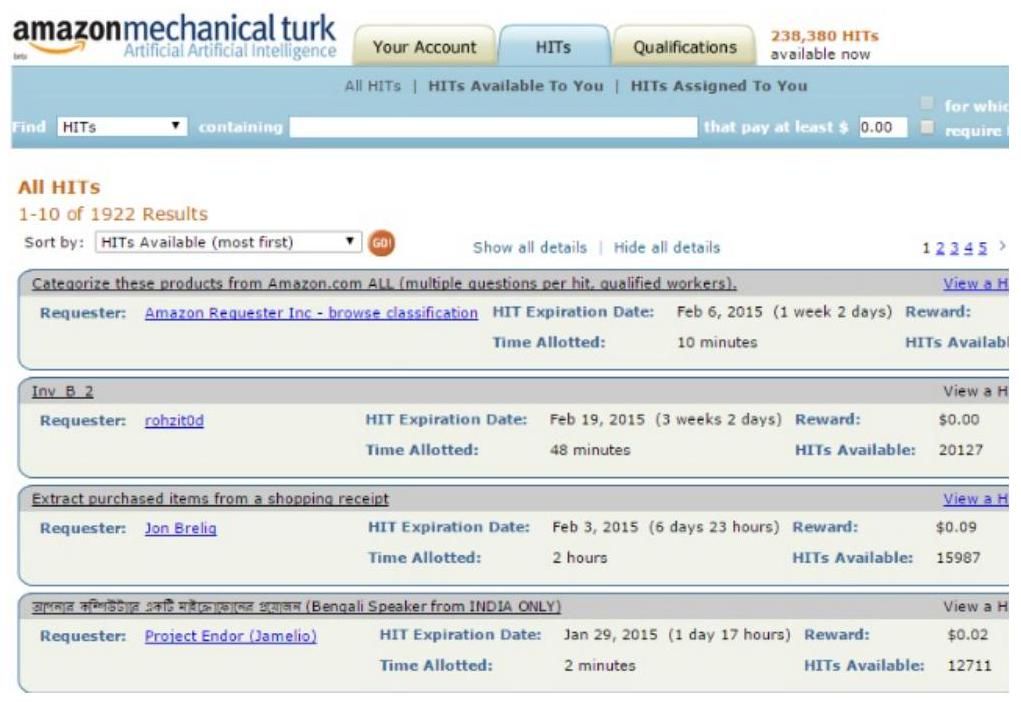
\includegraphics[max width=\textwidth]{2025_03_17_ca60ec0bfd96dcf8e028g-102}
    \caption{Representative tasks on Mechanical Turk.}
\end{figure}

कार्य जो टर्कर्स को सौंपे गए हैं वे सामान्यतः साधारण संज्ञानात्मक प्रयासों में शामिल होते हैं जिन्हें अभी तक कंप्यूटर द्वारा अच्छी तरह से नहीं किया जा सकता। टर्कर्स के अच्छे उपयोगों में शामिल हैं:

\begin{itemize}
  \item \textit{मानव धारणा के पहलुओं का मापन}: क्राउडसोर्सिंग सिस्टम सरल कार्यों पर प्रतिनिधि राय एकत्र करने के लिए कुशल तरीके प्रदान करते हैं। एक अच्छा अनुप्रयोग लाल-हरे-नीले स्पेस में रंगों के बीच संबंध स्थापित करना और उन नामों को पहचानना है जिनके द्वारा लोग आमतौर पर उन्हें एक भाषा में पहचानते हैं। उत्पादों और छवियों का विवरण लिखते समय यह जानना महत्वपूर्ण है।\\\index{bar charts}\index{bubble plots}\index{chart types!bar charts}\index{chart types!pie charts}\index{pie charts}\index{scatter plots!three-dimensional}
  तो रंग स्पेस में "नीला" और "हल्का नीला," या "रॉबिन के अंडे का नीला" और "टीएएल" के बीच सीमा कहाँ है? सही नाम संस्कृति और परंपरा का कार्य हैं, भौतिकी का नहीं। यह जानने के लिए, आपको लोगों से पूछना चाहिए, और क्राउडसोर्सिंग आपको आसानी से सैकड़ों या हज़ारों अलग-अलग लोगों से पूछताछ करने की अनुमति प्रदान करता है।
  \item \textit{मशीन लर्निंग वर्गीकर्ताओं के लिए प्रशिक्षण डेटा प्राप्त करना}: क्राउडसोर्सिंग में हमारी प्राथमिक रुचि मानव एनोटेशन का उत्पादन करने में होगी जो प्रशिक्षण डेटा के रूप में कार्य करेंगी। कई मशीन लर्निंग समस्याएं एक विशेष कार्य "वैसा ही करने की कोशिश करती हैं जैसा लोग करते हैं।" ऐसा करने के लिए बड़ी संख्या में प्रशिक्षण इंस्टेंस की आवश्यकता होती है ताकि यह स्थापित किया जा सके कि लोगों ने क्या किया, जब उन्हें मौका दिया गया।\\\index{heatmaps}
  उदाहरण के लिए, मान लें कि हम एक सेंटिमेंट एनालिसिस सिस्टम बनाना चाहते थे जो लिखित समीक्षाओं को पढ़ सके और यह तय कर सके कि किसी उत्पाद की राय अनुकूल है या प्रतिकूल। हमें परीक्षात्मक/प्रशिक्षण डेटा के रूप में काम करने के लिए एनोटेटरों द्वारा लेबल किए गए बड़े संख्या में समीक्षाओं की आवश्यकता होगी। इसके अलावा, हमें विभिन्न एनोटेटरों द्वारा बार-बार लेबल किए गए वही समीक्षाएँ चाहिए, ताकि
\end{itemize}

%---- Page End Break Here ---- Page : 85

\begin{itemize}
\item \textit{कंप्यूटर सिस्टम के लिए मूल्यांकन डेटा प्राप्त करना:} \textit{ए/बी परीक्षण} उपयोगकर्ता इंटरफेस को बेहतर बनाने का एक मानक तरीका है: एक दिए गए सिस्टम के संस्करण \textit{ए} को आधे जजों को दिखाएं और दूसरे आधे को संस्करण \textit{बी}। फिर जाँचें कि कौन सा समूह बेहतर करता है। टुरकर्स एक दिए गए ऐप की रुचिकरता या एक नए वर्गीकर्ता के प्रदर्शन पर प्रतिक्रिया प्रदान कर सकते हैं।\\\index{bar charts!best practices}\index{bar charts!stacked}\index{pie charts!best practices}
मेरे एक ग्रेड छात्र (यांकिंग चेन) ने क्राउडफ्लावर का उपयोग किया जो उसने बनाया था एक सिस्टम के मूल्यांकन के लिए जो किसी विशेष इकाई के लिए सबसे प्रासंगिक विकिपीडिया श्रेणी की पहचान करता है। बाराक ओबामा को कौन सी श्रेणी बेहतर वर्णित करती है: \textit{संयुक्त राज्य अमेरिका के राष्ट्रपति} या \textit{अफ्रीकी-अमेरिकी लेखक}? \$200 में, उसने लोगों से प्राप्त किए 10,000 ऐसे बहुविकल्पीय प्रश्नों के उत्तर, जो उसके सिस्टम का सही ढंग से मूल्यांकन करने के लिए पर्याप्त था।
\item \textit{मशीन में मनुष्यों का समावेश:} अब भी कई संज्ञानात्मक कार्य हैं जो लोग मशीनों की तुलना में बहुत बेहतर करते हैं। एक चतुराई से डिजाइन किया गया इंटरफेस कंप्यूटर के अंदर बैठे लोगों को जरूरतमंदों की सेवा करने के लिए उपयोगकर्ता प्रश्न प्रदान कर सकता है।\\
मान लीजिए कि आप एक ऐप बनाना चाहते हैं जो दृष्टिहीन व्यक्तियों की मदद कर सके, जिससे उपयोगकर्ता एक तस्वीर खींच सके और किसी से मदद मांग सके। शायद वे अपनी रसोई में हैं, और उन्हें किसी से डिब्बे पर लेबल पढ़वाना है। यह ऐप किसी टुरकर को उपप्रक्रिया के रूप में कॉल कर सकता है, जब भी ऐसा कार्य आवश्यक हो।\\
बेशक, इन छवि-अनोटेशन जोड़ों को भविष्य के विश्लेषण के लिए संग्रहित किया जाना चाहिए। वे मशीन लर्निंग प्रोग्राम के लिए प्रशिक्षण डेटा के रूप में काम कर सकते हैं, ताकि जितना संभव हो सके लोगों को प्रक्रिया से बाहर किया जा सके।
\item \textit{स्वतंत्र रचनात्मक प्रयास:} मांग पर बड़ी मात्रा में रचनात्मक कार्यों को कमीशन करने के लिए क्राउडसोर्सिंग का उपयोग किया जा सकता है। आप मांग पर ब्लॉग पोस्ट या लेख, या उत्पाद की लिखित समीक्षा अच्छी और बुरी, को ऑर्डर कर सकते हैं। जो कुछ भी आप कल्पना कर सकते हैं, वह बनाया जा सकता है, यदि आप केवल यह निर्दिष्ट करें कि आप क्या चाहते हैं।\\
मेरे पास दो मूर्खतापूर्ण उदाहरण हैं जिन्हें मैं किसी तरह प्रेरणादायक पाता हूँ:
\begin{itemize}
\item \textbf{द शीप मार्केट} (\href{http://www.thesheepmarket.com}{http://www.thesheepmarket.com}) ने प्रत्येक के लिए पैसे में 10,000 भेड़ों की ड्राइंग कमीशन की। एक अवधारणात्मक कला रचना के रूप में, यह उन्हें उच्चतम बोलीदाता को बेचने का प्रयास करता है। आप कौन से रचनात्मक प्रयास सोच सकते हैं जिन्हें लोग आपके लिए \$0.25 प्रति कार्य में करेंगे?
\item \textbf{इमोजी डिक} (\href{http://www.emojidick.com}{http://www.emojidick.com}) महान अमेरिकी उपन्यास \textit{मोबी डिक} को पूरी तरह इमोजी चित्रों में अनुवाद करने का एक भीड़-आधारित प्रयास था। इसके निर्माताओं ने पुस्तक को लगभग 10,000 भागों में विभाजित किया, और इनमें से प्रत्येक भाग को अनुवाद करने के लिए तीन अलग-अलग टुरकरों को दिया गया। अन्य टुरकरों को इन्हें अंतिम पुस्तक में शामिल करने के लिए सर्वश्रेष्ठ चुनने के लिए नियुक्त किया गया। इसमें 800 से अधिक टुरकर शामिल थे, और कुल खर्च \$3,676 था जिसे भीड़-धन साइट किकस्टार्टर द्वारा जुटाया गया।
\end{itemize}

\item\textit{आर्थिक/मनोवैज्ञानिक प्रयोग:}सामाजिक वैज्ञानिकों के लिए भीड़-स्रोतिंग व्यवहारिक अर्थशास्त्र और मनोविज्ञान के प्रयोगों के लिए वरदान साबित हुई है। स्थानीय स्नातकों को अपने अध्ययनों में भाग लेने के लिए प्रेरित करने के बजाय, ये शोधकर्ता अब अपने विषय पूल को पूरी दुनिया तक विस्तारित कर सकते हैं। उन्हें बड़ी जनसंख्या को आकर्षित करने की शक्ति मिलती है, विभिन्न देशों में स्वतंत्र पुनरावृत्ति करने की क्षमता मिलती है, और इस प्रकार वे जान सकते हैं कि उनके परिकल्पनाओं में कोई सांस्कृतिक पूर्वाग्रह है या नहीं।
\end{itemize}

भीड़-स्रोत का लाभ उठा कर काफ़ी रोमांचक कार्य सफलतापूर्वक पूरे किए जा सकते हैं। हालाँकि, यदि आप गलत तरीके से, गलत कार्य के लिए टर्कर्स का उपयोग करें, तो आप निराशा के लिए अभिशप्त हैं। भीड़-स्रोत के गलत उपयोग में शामिल हैं:

\begin{itemize}
\item \textit{कोई भी कार्य जो उन्नत प्रशिक्षण की आवश्यकता रखता है:} हालांकि हर व्यक्ति के पास अनूठी क्षमताएँ और विशेषज्ञता होती है, लेकिन क्राउडसोर्सिंग श्रमिकों के पास कोई विशेष प्रशिक्षण नहीं होता। उन्हें ऐसे हिस्सों के रूप में देखा जाता है जिन्हें आपस में बदल कर सकते हैं। आप इन श्रमिकों के साथ व्यक्तिगत संबंध स्थापित नहीं करते हैं, और कोई भी समझदारी से गिग इतना छोटा होगा कि कुछ मिनटों से अधिक प्रशिक्षण की अनुमति नहीं देगा।\\
ऐसे कार्य जो विशिष्ट तकनीकी कौशल की आवश्यकता रखते हैं, उन्हें क्राउडसोर्सिंग के माध्यम से नहीं करवाना व्यावहारिक होता है। हालांकि, उन्हें पारंपरिक, दीर्घकालिक व्यवस्था में समझदारी से उपकार्य के रूप में दिया जा सकता है।
\item \textit{कोई भी कार्य जिसे आप स्पष्ट रूप से नहीं निर्दिष्ट कर सकते:} आपके पास टर्कर्स के साथ संवाद का कोई तंत्र नहीं है। सामान्य रूप से, उनके पास आपसे प्रश्न पूछने का कोई तरीका नहीं होता। इसलिए यह प्रणाली केवल तभी काम करती है जब आप अपने कार्यों को स्पष्ट, संक्षेप और अस्पष्टता रहित निर्दिष्ट कर सकते हैं।\\
यह जितना दिखता है उससे कठिन होता है। समझें कि आप लोगों को प्रोग्राम करने की कोशिश कर रहे हैं न कि कम्प्यूटर को, जिसमें सभी attendant bugs होते हैं जो “जैसा मैं कहता हूँ वैसे करो” को “जैसा मैं मतलब करता हूँ वैसा नहीं” से ऊपर रखते हैं। अपने विनिर्देशों का स्थानीय लोगों पर परीक्षण करें इससे पहले कि आप अपनी नौकरी को भीड़ के लिए खोलें, और फिर अपने क्राउडसोर्सिंग प्लेटफॉर्म पर एक छोटा परीक्षण करें यह जानने के लिए कि यह कैसा जाता है, इससे पहले कि आप अपने बजट को खुला छोड़ दें। आपको कुछ सांस्कृतिक आश्चर्य मिल सकते हैं। जो बातें आपको स्पष्ट लगती हैं, वे आपके से आधे विश्व दूर के मजदूर के लिए कुछ बिल्कुल अलग का मतलब हो सकती हैं।
\item \textit{कोई भी कार्य जहां आप यह नहीं सत्यापित कर सकते कि वे अच्छा काम कर रहे हैं या नहीं:} टर्कर्स आपके टुकड़े-टुकड़े किए गए काम को लेने के लिए एकमात्र प्रेरणा से प्रेरित होते हैं: वे अपनी समय को पैसे में बदलने का प्रयास कर रहे हैं जितना efficiently संभव हो सके। वे ऐसे काम देख रहे हैं जो सबसे अच्छा buck for their bang देते हैं, और सबसे स्मार्ट लोग आपका कार्य जितनी जल्दी और बिना सोचे-समझे संभव हो सके पूरा करने के प्रयास में होंगे।\\\index{chart types!data maps}\index{U.S. presidential elections}
क्राउडसोर्सिंग प्लेटफॉर्म नियोक्ताओं को भुगतान रोक रखने की अनुमति देते हैं अगर अनुबंधित कार्य स्वीकार्य नहीं है। इसका फायदा उठाने के लिए उत्पाद की गुणवत्ता जांचने का कुछ प्रभावी तरीका होना आवश्यक है। शायद आपको उनसे कुछ कार्य पूरा करने के लिए कहना चाहिए जिसकी सही जवाब आपके पास पहले से हो। शायद आप उनके उत्तरों की तुलना अन्य स्वतंत्र श्रमिकों से कर सकते हैं, और यदि उनका काम अक्सर सहमति से असहमति में आता है तो उसे बाहर निकाल सकते हैं।
\end{itemize}

%---- Page End Break Here ---- Page : 87

\subsection{गेमिफिकेशन}\index{histograms!best practices}

यह अत्यंत महत्वपूर्ण है कि कुछ गुणवत्ता नियंत्रण तंत्र अपनाए जाएँ। किसी भी मंच पर उपलब्ध श्रमिकों का कुछ हिस्सा बॉट्स होते हैं, जो यादृच्छिकता के ज़रिए बहुविकल्पीय कार्यों पर आक्रमण करने की तलाश में रहते हैं। अन्य लोग हो सकते हैं जिनकी भाषा कौशल दी गई कार्य के लिए पूर्णतः अनुपयुक्त हो। आपको धोखा खाने से बचने के लिए जाँच और अस्वीकृति करनी होगी।

हालाँकि, आप खराब तरीके से निर्दिष्ट कार्यों से प्राप्त परिणामों की निष्पक्षता से शिकायत नहीं कर सकते। काम के बहुत अधिक हिस्से को अस्वीकार करने से आपकी प्रतिष्ठा पर असर पड़ेगा, कर्मचारियों और मंच के साथ। लोगों को भुगतान करने से इंकार करना लेकिन फिर भी उनके कार्य उत्पाद का उपयोग करना विशेष रूप से बुरा कर्म है।



शैक्षिक और अनुसंधान संस्थानों में लोग कानून से ज्यादा ऊँचे मानकों पर रखे जाते हैं, उनके \textit{संस्थागत समीक्षा बोर्ड} या आईआरबी के माध्यम से। आईआरबी शोधकर्ताओं और प्रशासनिक अधिकारियों की एक समिति होती है जो मानव विषयों पर किसी भी शोध को अनुमोदित करने के लिए आवश्यक होती है। हमारे द्वारा चर्चा किए गए जैसे निर्दोष क्राउडसोर्सिंग अनुप्रयोगों को नियमित रूप से अनुमोदित किया जाता है, खासकर तब जब शोधकर्ता ने यह सुनिश्चित करने के लिए एक संक्षिप्त ऑनलाइन प्रशिक्षण पाठ्यक्रम पूरा किया होता है कि वे नियमों को समझते हैं। \index{cartograms}\index{visualization!critiquing}

हमेशा समझें कि मशीन के दूसरी ओर एक व्यक्ति होता है। उन्हें ऐसे कार्य न सौंपें जो अपमानजनक, अवमाननापूर्ण, गोपनीयता-उल्लंघन करने वाले, या अत्यधिक तनावपूर्ण हों। यदि आप अपने कर्मचारियों के साथ मानवीय व्यवहार करेंगे तो आपको संभवतः बेहतर परिणाम मिलेंगे।
\end{itemize}

लोगों को आपके निर्देश मानने के लिए सही प्रोत्साहन की आवश्यकता होती है, केवल स्पष्ट निर्देश पर्याप्त नहीं होते। जीवन में, आमतौर पर आपको वही मिलता है जिसके लिए आप भुगतान करते हैं। अपने देश में वर्तमान में प्रचलित न्यूनतम प्रति घंटा वेतन के बारे में जानकारी रखें और उसके अनुसार अपने कार्यों का मूल्य निर्धारण करें। यह कोई कानूनी आवश्यकता नहीं है, लेकिन यह सामान्यतः अच्छा व्यापार होता है।

जिस भयावह चमक का अनुभव होता है जब आप श्रमिकों को प्रति घंटा\$0.50 पर काम पर रखते हैं, वह जल्दी ही ख़त्म हो जाती है जब आप देखते हैं कि आपके कार्यों के लिए जो श्रमिक आकर्षित होते हैं उनकी गुणवत्ता कितनी कम होती है। आप उनके कार्य उत्पाद को कठोरता से सही करने की आवश्यकता के कारण अपने सभी बचत को आसानी से ख़त्म कर सकते हैं, शायद इसे बार-बार करने के लिए कई श्रमिकों को भुगतान करके। उच्च भुगतान वाले कार्य श्रमिकों को बहुत तेजी से पाते हैं, इसलिए तैयार रहें यदि आप प्रचलित दर का भुगतान नहीं करते हैं तो प्रतीक्षा करनी पड़ सकती है। बॉट्स और उनके कार्यात्मक समकक्ष गुलामी जैसा वेतन स्वीकार करने में अधिक खुश होते हैं बजाय उन श्रमिकों के जिन्हें आप वास्तव में काम पर रखना चाहते हैं।



लोगों को आपके डेटा को एनोटेट या ट्रांसक्राइब करने के लिए भुगतान करने का एक विकल्प है। इसके बजाय, चीज़ों को इतना मज़ेदार बना दीजिए कि लोग आपके लिए मुफ्त में काम करने के लिए तैयार हो जाएं!

\textit{उद्देश्यपूर्ण खेल} (GWAP) वे प्रणालियाँ हैं जो डेटा संग्रह को एक ऐसे खेल के रूप में छुपाती हैं जिसे लोग खेलना चाहते हैं, या ऐसा कार्य जिसे लोग स्वयं करना चाहते हैं। खेल, प्रेरणा, और कल्पना के सही संयोजन के साथ, अद्भुत चीजें की जा सकती हैं। सफल उदाहरणों में शामिल हैं:



रेCAPTCHA का आविष्कार दैनिक रूप से प्रदर्शित 100 मिलियन से अधिक CAPTCHA से उपयोगी डेटा प्राप्त करने के लिए किया गया था। प्रत्येक में दो पाठ स्ट्रिंग्स दिखाई जाती हैं, जिनमें से एक को सिस्टम एंट्री प्रदान करने के लिए जांचता है। दूसरी पुराने किताबों और समाचार पत्रों को डिजिटाइज करने वाले ओसीआर प्रणाली के लिए एक कठिन मामला प्रस्तुत करती है। उत्तरों को वापस मानचित्रित किया जाता है ताकि पुरालेख दस्तावेजों के डिजिटलीकरण में सुधार हो सके, जिससे प्रतिदिन 40 मिलियन से अधिक शब्दों का प्रतिलेखन हो सके।
    
\item\textit{खेल/ऐप्स में मनोवैज्ञानिक/आईक्यू परीक्षण:}\index{IQ testing}मनोवैज्ञानिकों \index{psychologists}ने पाँच बुनियादी व्यक्तित्व लक्षणों को व्यक्तित्व के महत्वपूर्ण और पुनरुत्पादनीय पहलुओं के रूप में स्थापित किया है। अकादमिक मनोवैज्ञानिक व्यक्तित्व परीक्षणों के बहुविकल्पीय टेस्ट का उपयोग करके यह मापते हैं कि प्रत्येक बड़े पाँच लक्षणों के साथ व्यक्तियों की स्थिति कैसे होती है: openness, conscientiousness, extroversion, agreeableness, और neuroticism।

इन सर्वेक्षणों को गेम ऐप्स में बदलकर ("आपके \textit{व्यक्तित्व} लक्षण क्या हैं?") मनोवैज्ञानिकों ने 75,000 से अधिक विभिन्न लोगों पर ⸨व्यक्तित्व⸩ माप प्राप्त किए हैं, साथ ही पसंद और व्यवहार पर अन्य डेटा भी। इसने व्यक्तित्व के मनोविज्ञान में कई रोचक मुद्दों का अध्ययन करने के लिए एक विशाल डेटा सेट तैयार किया है।

\item\textit{प्रोटीन संरचनाओं की भविष्यवाणी के लिए फोल्डइट गेम:}\index{FoldIt}प्रोटीन अणुओं द्वारा बनाई गई संरचनाओं की भविष्यवाणी करना विज्ञान में महान संगणकीय चुनौतियों में से एक है। कई वर्षों के कार्य के बावजूद, क्या एक प्रोटीन को किसी विशेष आकार में मोड़ता है, यह अभी भी अच्छी तरह से समझा नहीं गया है।

फ़ोल्डइट (\href{https://fold.it}{https://fold.it}) एक खेल है जो गैर-जीवविज्ञानी लोगों को प्रोटीन अणुओं को एक विशेष आकार में मोड़ने के लिए चुनौती देता है। खिलाड़ियों को उनके डिज़ाइन की दी गई लक्ष्य के कितने करीब है उसके आधार पर अंक दिए जाते हैं, और उच्चतम अंक प्राप्त करने वाले खिलाड़ियों को एक लीडर बोर्ड पर रैंक किया जाता है। कई वैज्ञानिक पेपर विजयी डिज़ाइनों की मजबूती पर प्रकाशित हो चुके हैं।
\end{itemize}

यहाँ सफलता की कुंजी एक ऐसा गेम बनाना है जो खेलने योग्य हो और लोकप्रिय बन सके। यह जितना दिखता है उससे कहीं कठिन है। ऍप स्टोर में लाखों मुफ्त ऍप्स हैं, जिनमें से अधिकांश गेम्स हैं। बहुत ही कम को कुछ सौ से अधिक लोग आज़माते हैं, जो डेटा संग्रह के दृष्टिकोण से रुचिकर बनाने के लिए पर्याप्त नहीं है। यह एक अतिरिक्त बाधा जोड़ता है कि गेम को खेलने योग्य बनाने के साथ-साथ रोचक वैज्ञानिक डेटा उत्पन्न करना चाहिए, जो इस कार्य को और भी कठिन बना देता है।

प्रेरणात्मक तकनीकों का प्रयोग खेलपने में सुधार के लिए किया जाना चाहिए। स्कोर रखना किसी भी खेल का एक महत्वपूर्ण हिस्सा है, और खेल को इस तरह से डिज़ाइन किया जाना चाहिए ताकि प्रदर्शन शुरू में तेजी से बढ़े, जिससे खिलाड़ी को आकर्षित किया जा सके। प्रगति बार्स...

%---- Page End Break Here ---- Page : 89

\section{अध्याय टिप्पणी}

द चार्ल्स बैबेज़ उद्धरण इस अध्याय की शुरुआत में उनकी पुस्तक\textit{फिलोसोफर के जीवन से कुछ अंश} से लिया गया है। मैं पाडुआ के ग्राफिक उपन्यास की सिफारिश करता हूँ, जो उनके कार्य और एडा लोवलेस के साथ उनके संबंध का मनोरंजक लेकिन अर्थपूर्ण (हालांकि काल्पनिक) परिचय प्रदान करता है।

कई पुस्तकें विशेष प्रोग्रामिंग भाषाओं में डेटा प्रबंधन के व्यावहारिक मामलों से संबंधित होती हैं। पाइथन में डेटा विज्ञान के लिए ओ'रिली की पुस्तकें विशेष रूप से उपयोगी हैं, जिसमें \cite{grus2015data}, \cite{mckinney2012python}.\index{Python} शामिल हैं।

हमारी जै-अलाई सट्टेबाजी प्रणाली की कहानी, जिसमें वेबसाइट स्क्रैपिंग की भूमिका शामिल है, मेरी पुस्तक\textit{Calculated Bets}\cite{ski2001calculated} में रिपोर्ट की गई है। यह पूर्वानुमान के लिए सिमुलेशन मॉडलों का निर्माण करने का एक त्वरित और मजेदार अवलोकन है, और यह अनुभाग 7.8 की युद्ध कहानी का विषय होगा।

अंतरिक्ष मिशनों की असफलताएँ गणनात्मक कंप्यूटिंग त्रुटियों के कारण लोकप्रिय मीडिया में अच्छी तरह से दर्ज की गई हैं। एरिअन 5 और मंगल जलवायु ऑर्बिटर अंतरिक्ष मिशनों पर चर्चा के लिए Gleick \cite{gleick1996bug} और Stephenson et al. \cite{smb1999} देखें।

सेल फोन में ऍक्सेलेरोमीटर का उपयोग करके भूकंप का पता लगाने का च clever विचार Faulkner et al. \cite{fch2014} से आता है। बड़ी संख्या में Flickr छवियों के प्रतिनिधि अध्ययन Kisilevich et al. \cite{kkk2010} में शामिल हैं।

कित्तूर \cite{kittur2008crowdsourcing} ने एमेज़न टर्क पर क्राउडसोर्सिंग उपयोगकर्ता अध्ययन के अनुभवों पर रिपोर्ट दी है। हमारे द्वारा क्राउडफ्लावर का उपयोग ऐतिहासिक व्यक्तियों के उपयुक्त वर्णन को पहचानने के लिए किया गया था, जिसे \cite{chen2015vector} में प्रस्तुत किया गया। शिक्षण में गेमिफिकेशन के तरीके \cite{deterding2011game, kapp2012gamification} में चर्चा की गई हैं। रिकैप्चस को वॉन आह्न एट अल. \cite{vamm2008} में प्रस्तुत किया गया है। मोबाइल ऐप्स के माध्यम से मनोवैज्ञानिक लक्षण डेटा का बड़े पैमाने पर संग्रहण कोसिन्सकी एट अल. \cite{kosinski2013private} के कारण है।

\section{अभ्यास}

% Mismatched: \subsectionname{Data Munging}



\item [3-2.]\textit{[5]}दो प्रमुख डेटा विज्ञान प्रोग्रामिंग भाषाओं में से दो का चयन करें, और निम्नलिखित कार्यों को हल करने के लिए दोनों में कार्यक्रम लिखें। आपको प्रत्येक कार्य के लिए कौन सी भाषा सबसे उपयुक्त लगी?

\begin{enumerate}
        \item हैलो वर्ल्ड!
        \item एक फाइल से संख्याएँ पढ़ें, और उन्हें क्रमबद्ध क्रम में प्रिंट करें।
        \item एक पाठ्य फाइल पढ़ें, और कुल शब्दों की संख्या गिनें।
        \item एक पाठ्य फाइल पढ़ें, और \textit{अद्वितीय} शब्दों की कुल संख्या गिनें।
        \item संख्याओं की एक फाइल पढ़ें, और उनका एक आवृत्ति हिस्टोग्राम प्लॉट करें।
        \item वेब से एक पेज डाउनलोड करें, और उसे स्क्रैप करें।
    \end{enumerate}

\item [3-3.]\textit{[3]}थोड़ी देर के लिए Python, R, और Matlab के साथ खेलें। आपको कौन सा सबसे अच्छा लगता है? प्रत्येक की ताकतें और कमजोरियाँ क्या हैं?

\item[3-4.]\textit{[5]}$n$व्यक्ति की ऊँचाई का एक डेटासेट निर्माण करें, जिनमें से$p\%$को अंग्रेज़ी (फीट) में और बाकियों को मैट्रिक (मीटर) माप में दर्ज किया गया हो। सांख्यिकीय परिक्षणों का उपयोग करें यह जाँचने के लिए कि क्या यह वितरण एक विधिपूर्वक मीटर में दर्ज रिकॉर्ड से भिन्न है।$n$और$p$के फलन के रूप में सीमा क्या है जहाँ यह स्पष्ट हो जाता है कि कोई समस्या है?
\end{enumerate}

\subsection{डेटा स्रोत}



\item [3-6.]\textit{[5]}निम्नलिखित में से एक या अधिक\textit{द क्वांट शॉप}चुनौतियों के लिए, प्रासंगिक डेटा स्रोत खोजें और उनकी गुणवत्ता का मूल्यांकन करें:

\begin{itemize}
        \item \textit{मिस यूनिवर्स।}
        \item \textit{फ़िल्म की कमाई।}
        \item \textit{बच्चे का वजन।}
        \item \textit{कला नीलामी की कीमत।}
        \item \textit{क्रिसमस पर बर्फ।}
        \item \textit{सुपर बाउल/कॉलेज चैंपियन।}
        \item \textit{घौल पूल?}
        \item \textit{भविष्य में सोने/तेल की कीमत?}
    \end{itemize}

\end{enumerate}

\subsection{डेटा क्लीनिंग}



\item [3-8.]\textit{[3]}आप निम्नलिखित डेटा सेट्स में किस प्रकार के औटलाईयर्स होने की उम्मीद कर सकते हैं:

\begin{enumerate}
        \item छात्र ग्रेड्स.
        \item वेतन डेटा.
        \item विकिपीडिया में जीवन अवधि.
    \end{enumerate}

\item [3-9.]\textit{[३]} एक स्वास्थ्य सेंसर बीस विभिन्न मानों की एक धारा उत्पन्न करता है, जिसमें रक्तचाप, हृदय गति, और शरीर का तापमान शामिल हैं। दो या अधिक तकनीकों का वर्णन करें जिनका आप यह जांचने के लिए उपयोग कर सकते हैं कि सेंसर से आ रही डेटा धारा मान्य है या नहीं।
\end{enumerate}

\subsection{कार्यान्वयन परियोजनाएँ}



\item [3-11.]\textit{[5]}संयुक्त राज्य अमेरिका में मतदाता पंजीकरण अभिलेखों को नियंत्रित करने वाले कानून राज्य से राज्य में भिन्न होते हैं। उन राज्यों में से एक या अधिक की पहचान करें जहाँ नियम बहुत उदार हैं, और देखें कि डेटा प्राप्त करने के लिए आपको क्या करना होगा। संकेत: फ्लोरिडा।
\end{enumerate}

% Mismatched: \subsectionname{Crowdsourcing}



\item [3-13.]\textit{[3]} मान लीजिए कि आप टर्कर्स को पाठ पढ़ने और उन्हें अंतर्निहित भावना (सकारात्मक या नकारात्मक) के आधार पर एनोटेट करने के लिए भुगतान कर रहे हैं जो प्रत्येक अंश व्यक्त करता है। यह एक राय का कार्य है, लेकिन हम एल्गोरिदमिक रूप से कैसे जाँच सकते हैं कि टर्कर यादृच्छिक या मनमाने ढंग से उत्तर दे रहा था या नहीं, बजाय इसके कि वह अपना काम गंभीरता से कर रहा हो?
\end{enumerate}

\subsection{साक्षात्कार प्रश्न}



\item [3-15.]\textit{[5]}आम तौर पर, आप बाहरी तत्वों के लिए कैसे जाँच करेंगे, और अगर आपको कोई मिले तो आपको क्या करना चाहिए?

\item [3-16.]\textit{[3]}डेटा सफाई विश्लेषण में महत्वपूर्ण भूमिका क्यों निभाती है?
\end{enumerate}

%---- Page End Break Here ---- Page : 92
Here is the LaTeX content formatted according to the JSON data and guidelines provided:



\begin{enumerate}
    \item[3-17.] \textit{[5]} विश्लेषण के दौरान, आप अनुपलब्ध मानों को कैसे संभालते हैं? 
    \item[3-18.] \textit{[5]} चयन पूर्वाग्रह की व्याख्या करें। यह क्यों महत्वपूर्ण है? आकड़ों के प्रबंधन की प्रक्रियाएँ जैसे अनुपलब्ध आकड़े संभालने से यह कैसे खराब हो सकता है? 
    \item[3-19.] \textit{[3]} आप वेब आकड़ों को कुशलता से कैसे स्क्रैप करते हैं? 
\end{enumerate}

% Mismatched: \sectionname{Kaggle Challenges}

\begin{enumerate}
    \item आंशिक रूप से धूप, हैशटैग्स की संभावना के साथ। \href{https://www.kaggle.com/c/crowdflower-weather-twitter}{\index{CrowdFlower}https://www.kaggle.com/c/crowdflower-weather-twitter}
    \item दिन के अंत के स्टॉक रिटर्न्स की भविष्यवाणी करें, बिना शोर से धोखा खाए। \\ \href{https://www.kaggle.com/c/the-winton-stock-market-challenge}{https://www.kaggle.com/c/the-winton-stock-market-challenge}
    \item डाटा क्लीनिंग और ऐतिहासिक जलवायु परिवर्तन का विश्लेषण। \\ \href{https://www.kaggle.com/berkeleyearth/climate-change-earth-surface-temperature-data}{https://www.kaggle.com/berkeleyearth/climate-change-earth-surface-temperature-data}
\end{enumerate}

\chapter{स्कोर और रैंकिंग}

पैसा एक स्कोरबोर्ड है जहाँ आप अन्य लोगों के मुकाबले अपनी प्रगति की रैंकिंग कर सकते हैं।

\begin{flushright}मार्क क्यूबन\end{flushright}

\section{स्कोरिंग फंक्शन्स का परिचय}

\textit{स्कोरिंग फंक्शन्स} वे उपाय हैं जो बहु-आयामी रिकॉर्ड्स को एकल मूल्य में बदल देते हैं, डेटा की किसी विशेष विशेषता को उजागर करते हुए। स्कोरिंग फंक्शन्स का एक परिचित उदाहरण वे हैं जो छात्रों को मेरे जैसे पाठ्यक्रमों में ग्रेड देने के लिए उपयोग किए जाते हैं। छात्र इन संख्यात्मक स्कोरों के अनुसार क्रमबद्ध (रैंक्ड) किए जा सकते हैं, और बाद में इस क्रम के आधार पर उन्हें पत्र ग्रेड दिए जाते हैं।

ग्रेड सामान्यतः संख्यात्मक विशेषताओं के ऊपर फ़ंक्शन्स द्वारा गणना की जाती हैं जो छात्र के प्रदर्शन को दर्शाती हैं, जैसे कि प्रत्येक होमवर्क और परीक्षा पर दिए गए अंक। प्रत्येक छात्र को एकल संयुक्त स्कोर प्राप्त होता है, जो अक्सर 0 और 100 के बीच स्केल किया जाता है। ये स्कोर आमतौर पर इनपुट वेरिएबल्स के रैखिक संयोजन से आते हैं, संभवतः पाँच होमवर्क असाइनमेंट्स में से प्रत्येक को 8\% भार देने और तीन परीक्षाओं में से प्रत्येक को 20\% भार देने के साथ।

ऐसी ग्रेडिंग रूब्रिक्स के बारे में कई चीजें देखने लायक हैं, जिन्हें हम अधिक सामान्य स्कोरिंग और रैंकिंग फंक्शन के लिए एक मॉडल के रूप में उपयोग करेंगे:

\begin{itemize}
  \item \textit{मनमानी की डिग्री:} हर शिक्षक/प्रोफेसर अपने छात्रों का मूल्यांकन करते समय गृहकार्य स्कोर और परीक्षाओं के बीच अलग-अलग संतुलन का उपयोग करते हैं। कुछ अंतिम परीक्षा को अन्य सभी चरों की तुलना में अधिक महत्व देते हैं। कुछ औसत निकालने से पहले प्रत्येक मूल्य को 100 तक सामान्यीकृत करते हैं, जबकि अन्य प्रत्येक स्कोर को एक Z-स्कोर में परिवर्तित करते हैं। वे सभी अपने दर्शन में भिन्न होते हैं, फिर भी हर शिक्षक/प्रोफेसर इस बात को लेकर निश्चित होता है कि उनका मूल्यांकन प्रणाली चीजों को करने का सबसे अच्छा तरीका है।
  \item \textit{मान्यकरण डेटा की कमी:} ऐसा कोई सोने का मानक नहीं है जो निर्देशकों को यह सूचित करे कि उनके छात्रों को पाठ्यक्रम में जो सही ग्रेड \textit{मिलना चाहिए} वह क्या है। छात्र अक्सर शिकायत करते हैं कि मुझे उन्हें बेहतर ग्रेड देना चाहिए, लेकिन इन अनुरोधों में स्वार्थ वस्तुनिष्ठता से अधिक प्रकट होता है। वास्तव में, मैंने शायद ही कभी छात्रों को यह सुझाव देते सुना है कि मुझे उनका ग्रेड कम करना चाहिए।
  \item \textit{सामान्य शक्ति:} और फिर भी, पूरी तरह से अलग और बिना मान्यताप्राप्त दृष्टिकोणों का उपयोग करने के बावजूद, विभिन्न मूल्यांकन प्रणालियाँ आम तौर पर समान परिणाम उत्पन्न करती हैं। हर स्कूल में सीधे A पाने वाले छात्रों का एक समूह होता है जो प्रत्येक पाठ्यक्रम में शीर्ष ग्रेड के बड़े हिस्से पर कब्जा करता है। ऐसा नहीं हो सकता यदि ये सभी विभिन्न मूल्यांकन प्रणालियाँ छात्र प्रदर्शन को मनमाने ढंग से क्रमबद्ध कर रही होती। सी ग्रेड पाने वाले आम तौर पर अपनी कक्षाओं के अधिकांश भाग में मध्य से निम्न स्तर पर रह जाते हैं, बजाय इसके कि वे अपने अंतिम औसत के रास्ते में A और F के बीच परिवर्तन करते रहें। सभी मूल्यांकन प्रणालियाँ अलग हैं, फिर भी लगभग सभी का बचाव किया जा सकता है।\index{bias}\index{bias–variance trade-off}\index{deep learning}\index{error}\index{modeling!underfit}\index{Occam, William of}\index{overfitting}\index{variance}
\end{itemize}

इस अध्याय में, हम डाटा विश्लेषण में अपनी पहली यात्रा के रूप में स्कोरिंग और रैंकिंग फंक्शन्स का उपयोग करेंगे। हर किसी को ये उतने पसंद नहीं आते जितना मुझे आते हैं। स्कोरिंग फंक्शन्स अक्सर मनमाने और अस्थायी लगते हैं, और गलत हाथों में यह प्रभावशाली दिखने वाले अंक उत्पन्न कर सकते हैं जो मूल रूप से निरर्थक होते हैं। क्योंकि इनकी प्रभावशीलता को सामान्यतः सत्यापित नहीं किया जा सकता, ये तकनीकें उतनी वैज्ञानिक रूप से मजबूत नहीं हैं जितनी सांख्यिकी और मशीन लर्निंग विधियाँ, जिन्हें हम आगामी अध्यायों में प्रस्तुत करेंगे।

लेकिन मुझे लगता है कि यह महत्वपूर्ण है कि स्कोरिंग फंक्शन्स की सराहना की जाए कि वे क्या हैं: बड़े डेटा सेट्स से समझ निकालने के लिए उपयोगी, हेयुरिस्टिक तरीकें। एक स्कोरिंग फंक्शन को कभी-कभी एक\textit{सांख्यिकी} कहा जाता है, जो इसे अधिक गरिमा और सम्मान प्रदान करता है। हम डेटा से सार्थक स्कोर्स प्राप्त करने के लिए कई विधियाँ पेश करेंगे।

\section{शरीर द्रव्यमान सूचकांक (बीएमआई)}

हर किसी को खाना पसंद है, और हमारी आधुनिक प्रचुर संसार खाने के अनेक अवसर प्रदान करता है। इसका परिणाम यह है कि जनसंख्या का एक बड़ा प्रतिशत उनके आदर्श शरीर वजन से अधिक है। लेकिन आप कैसे जान सकते हैं कि आप उनमें से एक हैं?\index{modeling!principles for effectiveness}\index{modeling!overfit}\index{probabilistic}\index{Silver, Nate}\index{U.S. presidential elections}

\textit{शरीर द्रव्यमान सूचकांक} (BMI) एक स्कोर या सांख्यिकी है जिसे यह समझने के लिए डिज़ाइन किया गया है कि आपका वजन नियंत्रण में है या नहीं। इसे परिभाषित किया गया है।

\[
BMI = \frac{\text{mass}}{\text{height}^{2}}
\]

जहाँ द्रव्यमान किलोग्राम में मापा जाता है और ऊँचाई मीटर में। जब मैं यह लिख रहा हूँ, मैं 68 इंच लंबा (1.727 मीटर) हूँ और 150 पाउंड (68.0 किलोग्राम) पर थोड़ा भारी महसूस कर रहा हूँ। इस प्रकार मेरा बीएमआई है\(68.0 / (1.727^{2}) = 22.8\)। हालाँकि, यह इतना बुरा नहीं है क्योंकि संयुक्त राज्य अमेरिका में आमतौर पर स्वीकृत बीएमआई सीमाएँ परिभाषित करती हैं:

\begin{itemize}
  \item \textit{अंडरवेट:} 18.5 से नीचे.
  \item \textit{सामान्य वजन:} 18.5 से 25 तक.
  \item \textit{अधिक वजन:} 25 से 30 तक.
  \item \textit{मोटापा:} 30 से ऊपर.
\end{itemize}

इस प्रकार मुझे सामान्य श्रेणी में गिना जाता है, और मुझे आधिकारिक रूप से वजन से अधिक होने से पहले एक दर्जन पाउंड और बढ़ाने की आवश्यकता है। चित्र~\ref{fig:bmi-plot} दर्शाता है कि इस मापदंड के अनुसार अमेरिकी लोगों का एक प्रतिनिधित्व समूह ऊँचाई-वजन के स्थान में कहाँ स्थित है। इस स्कैटर प्लॉट के प्रत्येक बिंदु एक व्यक्ति का प्रतिनिधित्व करते हैं, जो उनके बीएमआई के अनुसार रंगित होते हैं। ठोस रंग के प्रतीत होने वाले क्षेत्र इतने घने हैं कि बिंदु एक-दूसरे के ऊपर जा रहे हैं। दाएँ ओर के बाहरी बिंदु सबसे भारी व्यक्तियों से संबंधित हैं।

बीएमआई एक बहुत ही सफल सांख्यिकी/स्कोरिंग फ़ंक्शन का उदाहरण है। यह व्यापक रूप से उपयोग किया जाता है और सामान्यतः स्वीकार किया जाता है, हालांकि सार्वजनिक स्वास्थ्य क्षेत्र के कुछ लोग इस पर यह कहकर आपत्ति जताते हैं कि बेहतर सांख्यिकी उपलब्ध हैं।

बीएमआई के लिए तर्क लगभग सही है। ऊंचाई का वर्ग \textit{क्षेत्रफल} के समानुपाती होना चाहिए। लेकिन भार को \text{आयतन} के समानुपाती बढ़ना चाहिए, न कि क्षेत्रफल के, तो यह क्यों नहीं है\(\text{भार}/{ऊंचाई}^{3}\)? ऐतिहासिक रूप से, बीएमआई को एक व्यक्ति के शरीर में वसा के प्रतिशत के साथ संबंध स्थापित करने के लिए डिज़ाइन किया गया था, जो ऊंचाई और वजन की तुलना में मापना कहीं अधिक कठिन होता है। कई सरल स्कोरिंग फ़ंक्शन्स के प्रयोग, जिनमें\(m / l\)और\(m / l^⸨3⸩\)शामिल थे, से पता चला कि बीएमआई सबसे अच्छा काम करता है।\index{Bayes’ theorem}\index{modeling!taxonomy of}

यह बहुत रोचक होता है कि चरम जनसंख्या के लिए बीएमआई वितरण को देखा जाए। पेशेवर खिलाड़ियों को अमेरिकी फुटबॉल (एनएफएल) और बास्केटबॉल (एनबीए) में सोचें:

\begin{itemize}
  \item \textit{बास्केटबॉल खिलाड़ी} असाधारण रूप से लंबे व्यक्ति होते हैं। उन्हें पूरे दिन कोर्ट पर ऊपर और नीचे दौड़ना भी पड़ता है, जिससे वे उत्कृष्ट फिटनेस हासिल करते हैं।
  \item \textit{अमेरिकी फुटबॉल खिलाड़ी} असाधारण रूप से भारी व्यक्ति होते हैं। विशेष रूप से, लाइनमेन केवल अन्य लाइनमेन को ब्लॉक करने या हटाने के लिए होते हैं, जिससे वजन पर प्राथमिकता रहती है।
\end{itemize}

आइए कुछ आंकड़ों पर नजर डालें। चित्र~\ref{fig:sport-bmi-dist}खेल के अनुसार बास्केटबॉल और फुटबॉल खिलाड़ियों के BMI वितरण को दिखाता है।

कृपया सुनिश्चित करें कि `\begin{figure}`...`\end{figure}` डालें और छवियों का सही संदर्भ दें `चित्र 4.1` (ऊँचाई-भार बिखराव प्लॉट) और `चित्र 4.2` (खेल के अनुसार बीएमआई वितरण) को LaTeX दस्तावेज़ में जैसा वे आपके द्वारा प्रबंधित सामग्री में दिखाई देती हैं।

\begin{figure}[htbp]
\centering
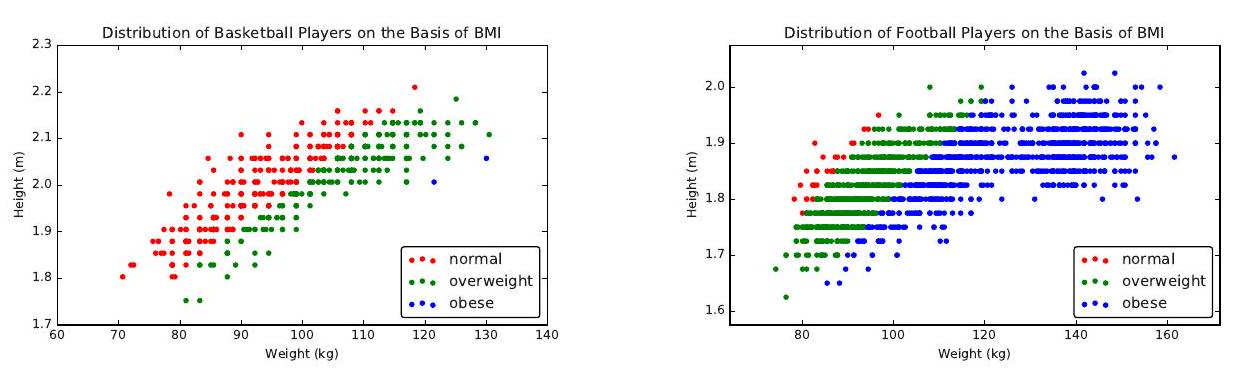
\includegraphics[max width=\textwidth]{2025_03_17_ca60ec0bfd96dcf8e028g-114(2)}
\caption{BMI distributions of professional basketball (left) and football (right) players.}
\end{figure}

\begin{figure}[htbp]
\centering
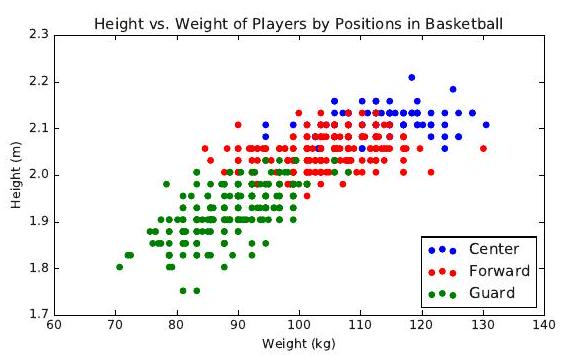
\includegraphics[max width=\textwidth]{2025_03_17_ca60ec0bfd96dcf8e028g-114(1)}
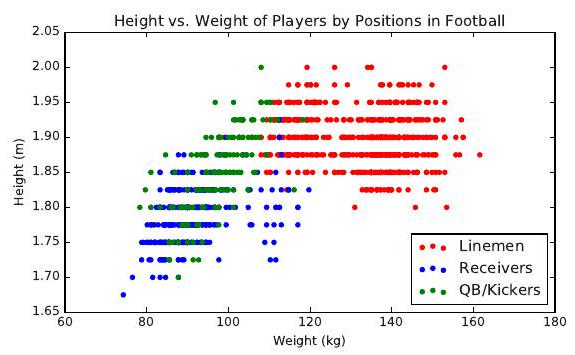
\includegraphics[max width=\textwidth]{2025_03_17_ca60ec0bfd96dcf8e028g-114}
\caption{Position in basketball (left) and football (right) is largely determined by size.}
\end{figure}

उनके बहुत ही असामान्य ऊँचाई होने के बावजूद भी उनका सामान्य बीएमआई है। और फुटबॉल खिलाड़ी लगभग समान रूप से जानवर समान होते हैं, ज्यादातर को अधिक वजन के रूप में अंकित किया गया है, इस तथ्य के बावजूद कि वे भी अच्छी तरह से प्रशिक्षित एथलीट होते हैं। ये फुटबॉल खिलाड़ी आमतौर पर शक्ति के लिए अनुकूलित होते हैं, बजाय कार्डियोवास्कुलर फिटनेस के।

अध्याय~\ref{अध्याय:दृश्यात्मकता}में, हम आँकड़ों की प्रस्तुति को उजागर करने के लिए दृश्यात्मक तकनीकों पर चर्चा करेंगे, लेकिन आइए यहाँ हमारे सौंदर्य का विकास करना शुरू करें। हम\textit{स्कैटर प्लॉट्स}का उपयोग करते हैं ताकि प्रत्येक व्यक्ति को ऊँचाई-भार स्पेस में एक बिंदु के रूप में दिखाया जा सके, जिसमें लेबल (भार वर्ग या खिलाड़ी की स्थिति) रंगों के रूप में दिखाए जाते हैं।

बीएमआई का पदानुसार विश्लेषण भी खुलासा करने वाला है, और इसे आकृति~4.3 में दिखाया गया है। बास्केटबॉल में, गार्ड्स तेज और छरहरे होते हैं जबकि सेंटर्स लंबे और डरावने होते हैं। इस प्रकार, सभी पद आकार के अनुसार साफ-सुथरे तरीके से अलग हो जाते हैं। फुटबॉल में, कौशल खिलाड़ी (क्वार्टरबैक, किकर्स और पंटर्स) मैदान की लाइन पर मांस के टुकड़ों की तुलना में काफी छोटे साबित होते हैं।

\section{स्कोरिंग सिस्टम विकसित करना}
\index{developing scoring systems}स्कोर वे फंक्शन होते हैं जो प्रत्येक इकाई की विशेषताओं को गुणात्मक मान में मैप करते हैं। इस खंड में प्रभावी स्कोरिंग सिस्टम बनाने और उनका मूल्यांकन करने के बुनियादी दृष्टिकोणों पर विचार किया जाएगा।\index{data-driven!models}\index{modeling!data-driven}\index{modeling!first-principle}

\subsection{गोल्ड स्टैंडर्ड्स और प्रॉक्सी}
\index{proxies}\index{gold standards}ऐतिहासिक रूप से, कागज़ी मुद्राएँ सोने द्वारा समर्थित होती थीं, जिसका मतलब था कि एक कागज़ का डॉलर हमेशा \$1 मूल्य का सोना के लिए बदला जा सकता था। यही कारण था कि हमें पता था कि हमारी मुद्रा उस कागज़ से अधिक मूल्यवान थी जिस पर यह मुद्रित थी।

डाटा विज्ञान में, a\textit{सुनहरा मानक} एक सेट होता है लेबल्स या उत्तरों का जिन पर हमें सही होने का विश्वास होता है। बीएमआई के मूल सूत्रीकरण में, सुनहरा मानक उन शारीरिक वसा प्रतिशतों का था जो कुछ गिने-चुने व्यक्तियों पर सावधानीपूर्वक मापे गए थे। निश्चित रूप से, ऐसे मापों में कुछ त्रुटि हो सकती है, लेकिन इन मानों को फिटनेस के लिए सुनहरा मानक मानकर, हम इन्हें सही माप मान लेते हैं। सोने में हम विश्वास करते हैं।

एक स्वर्ण मानक की उपस्थिति एक अच्छा स्कोरिंग प्रणाली विकसित करने के लिए एक कठोर तरीका प्रदान करती है। हम लाइनियर रिग्रेशन जैसी वक्र-फिटिंग तकनीकों का उपयोग कर सकते हैं (जिस पर \ref{sec:linear_regression} खंड में चर्चा की जाएगी) इनपुट फीचरों को इस तरह से तोलने के लिए कि स्वर्ण मानक उदाहरणों पर "सही उत्तरों" का सर्वोत्तम सन्निकटन हो सके।

लेकिन असली \textit{सोने} के मानक खोजना मुश्किल हो सकता है। ⸨प्रॉक्सी⸩ वे डेटा होते हैं जिन्हें खोजना आसान होता है और जो वांछित लेकिन अप्राप्य भूमि सत्य के साथ अच्छे से संबंध रखते हैं। बीएमआई को शरीर की चर्बी के प्रतिशत के लिए एक प्रॉक्सी के रूप में डिजाइन किया गया था। इसे केवल ऊँचाई और वजन से आसानी से गणना किया जा सकता है, और यह शरीर की चर्बी के साथ काफी अच्छा संबंध रखता है। इसका मतलब है कि पानी की टंकियों में अस्थायित्व का परीक्षण करना या कैलीपर्स के साथ "इंच को पिंच करना" जैसे अधिक अवरोधक उपायों को शायद ही कभी आवश्यक होता है, जो सीधे तौर पर व्यक्ति की चर्बी की मात्रा को मापते हैं।

मान लीजिए कि मैं अगले वर्ष के डाटा साइंस कोर्स के लिए अपने ग्रेडिंग सिस्टम को सुधारना चाहता हूँ। मेरे पास पिछले वर्ष के छात्रों का डाटा है, जिसमें उनके होमवर्क और परीक्षणों पर प्राप्त अंक शामिल हैं, लेकिन मेरे पास वास्तव में कोई सुनहरा मानक नहीं है कि इन छात्रों को कौन से ग्रेड \textit{मिलने चाहिए}। मेरे पास केवल वह ग्रेड है जो मैंने उन्हें दिया था, जो इस सिस्टम को सुधारने की कोशिश में अर्थहीन है।

मुझे उनके अज्ञात "वास्तविक" पाठ्यक्रम योग्यता के लिए एक प्रॉक्सी चाहिए। इसके लिए एक अच्छा उम्मीदवार प्रत्येक छात्र का\textit{अन्य}पाठ्यक्रमों में संचयी जीपीए हो सकता है। सामान्य तौर पर, छात्रों का प्रदर्शन पाठ्यक्रमों में संरक्षित होना चाहिए। यदि मेरी स्कोरिंग प्रणाली सबसे अच्छे छात्रों के जीपीए को नुकसान पहुँचाती है और निचले स्तर के छात्रों की मदद करती है, तो शायद मैं कुछ गलत कर रहा हूँ।

प्रॉक्सी विशेष रूप से अच्छे होते हैं जब स्कोरिंग/रैंकिंग सिस्टम का मूल्यांकन किया जाता है। हमारी किताब \textit{Who’s Bigger?}~\cite{SW13} में हमने विकिपीडिया का उपयोग करके ऐतिहासिक व्यक्तित्वों को "महत्त्व" के अनुसार रैंक किया। हमारे पास यह मापने के लिए कोई स्वर्ण मानक महत्त्व डेटा नहीं था कि ये लोग \textit{वास्तव में} कितने महत्त्वपूर्ण थे। लेकिन हमने अपनी ईमानदारी बनाए रखने के लिए कई प्रॉक्सी का उपयोग किया:

\begin{itemize}
  \item मशहूर हस्तियों के हस्ताक्षरों के लिए संग्राहकों द्वारा दी जाने वाली कीमतें \textit{अमूमन} उस हस्ती के महत्व के साथ मेल खानी चाहिए। जितनी अधिक कीमत लोग देने को तैयार होते हैं, उतना बड़ा सितारा होता है।
  \item एक बेसबॉल खिलाड़ी कितना अच्छा है, इसके आँकड़े \textit{अमूमन} खिलाड़ी के महत्व के साथ मेल खाने चाहिए। जितना बेहतर खिलाड़ी, उतना अधिक महत्वपूर्ण होने की संभावना।\index{deep learning!models}\index{discounting}\index{modeling!deep learning}\index{modeling!flat}\index{modeling!hierarchical}
  \item किताबों और पत्रिकाओं में प्रकाशित रैंकिंग्स शीर्ष राष्ट्रपतियों, फिल्मी सितारों, गायकों, लेखकों आदि की सूची बनाती हैं। इतिहासकारों द्वारा उच्च रैंकिंग प्राप्त राष्ट्रपतियों को आम तौर पर हमें भी उच्च स्थान देना चाहिए। ऐसे विचार, समग्र रूप से, इन ऐतिहासिक व्यक्तित्वों के महत्व के साथ ⸨अमूमन\end{itemize} मेल खाने चाहिए।
⸩

हम हमारे ऐतिहासिक महत्व स्कोर्स के कार्यप्रणाली पर अधिक विस्तार से धारा~\ref{sec:historical_significance} में चर्चा करेंगे।

\subsection{अंक बनाम रैंकिंग्स}
\textit{रैंकिंग्स} गुण के आधार पर n संस्थाओं की क्रम व्यवस्था होती है, जिन्हें आमतौर पर किसी अंक प्रणाली के परिणाम को क्रमबद्ध करके तैयार किया जाता है। रैंकिंग्स/रेटिंग प्रणाली के लोकप्रिय उदाहरण शामिल हैं:



%---- Page End Break Here ---- Page : 100







$A = 4.0)$. लेकिन प्राकृतिक रूप से अलग-अलग रूप होते हैं: कई स्कूल सम्मानित पाठ्यक्रमों को लाइटवेट कक्षाओं जैसे जिम की तुलना में अधिक गंभीरता से तौलने का विकल्प चुनते हैं, ताकि अच्छे ग्रेड प्राप्त करने की अधिक कठिनाई को दर्शाया जा सके।

सामान्य रूप से, किसी स्कोरिंग सिस्टम के परिणामों को सॉर्ट करने से एक संख्यात्मक रैंकिंग प्राप्त होती है। लेकिन दूसरी ओर सोचते हुए, प्रत्येक आइटम की रैंकिंग स्थिति (जैसे, 2196 में से 493वाँ) भी आइटम के लिए एक संख्यात्मक स्कोर प्राप्त करती है।

क्योंकि स्कोर और रैंकिंग एक-दूसरे के द्वंद्व होते हैं, कौन सा डेटा का अधिक अर्थपूर्ण प्रतिनिधित्व प्रदान करता है? जैसे किसी भी तुलना में, सबसे अच्छा उत्तर यह होता है कि यह निर्भर करता है, जैसे मुद्दों पर:

\begin{itemize}
  \item \textit{क्या संख्याएँ अलगाव में प्रस्तुत की जाएंगी?} रैंकिंग स्कोर की व्याख्या के लिए संदर्भ प्रदान करने में अच्छी होती हैं। जैसा कि मैं इसे लिख रहा हूँ, स्टोनी ब्रूक की बास्केटबॉल टीम का राष्ट्रीय 351 कॉलेज टीमों के बीच 111वां स्थान है, हमारे आरपीआई (रेटिंग्स प्रतिशत सूचकांक) 39.18 के आधार पर। कौन सी संख्या आपको यह समझने में बेहतर मदद करती है कि हमारी टीम अच्छी है या बुरी, 111वां या 39.18?
  \item \textit{स्कोर का मूल वितरण क्या है?} परिभाषा के अनुसार, शीर्ष रैंक वाली इकाई का स्कोर दूसरे रैंक वाली से बेहतर होता है, लेकिन इससे आपको उनके बीच के अंतर की मात्रा के बारे में कुछ नहीं पता चलता। क्या वे वास्तव में बराबर हैं, या \#1 इसमें हावी हो रही है?
\end{itemize}

\index{Occam’s razor}
रैंकिंग में अंतर \textit{दिखाई देते}हैं कि वे रैखिक हैं: 1 और 2 के बीच का अंतर 111 और 112 के बीच के अंतर के समान लगता है। लेकिन स्कोरिंग प्रणाली में यह आमतौर पर सही नहीं होता है। वास्तव में, छोटे परिपूर्ण स्कोरिंग अंतर अक्सर बड़े रैंकिंग अंतरों का परिणाम हो सकते हैं।\index{classification!evaluating}\index{negative class}\index{positive class}

\begin{itemize}
  \item \textit{क्या आप चरम सीमा के बारे में परवाह करते हैं या बीच के बारे में?} अच्छी तरह से डिजाइन किए गए स्कोरिंग सिस्टम अक्सर एक बेल के आकार के वितरण रखते हैं। औसत के आसपास स्कोर के संकेन्द्रण के साथ, स्कोर में छोटे अंतर रैंक में बड़े अंतर का मतलब हो सकते हैं। एक सामान्य वितरण में, औसत से अपने स्कोर को एक मानक विचलन ($\sigma$) बढ़ाकर आप को 50वीं प्रतिशतक से 84वीं प्रतिशतक पर ले जाता है। लेकिन $1\sigma$ से $2\sigma$ तक बदलाव का वही आकार आपको केवल 84वीं से 92.5वीं प्रतिशतक तक ले जाता है।
\end{itemize}

इसलिए जब कोई संगठन पहले स्थान से दसवें स्थान पर खिसकता है, तो अधिकारियों को जवाबदेह ठहराया जाना चाहिए। लेकिन जब स्टॉनी ब्रूक की टीम 111वें से 120वें स्थान पर जाती है, तो यह संभवतः स्कोर में एक तुच्छ अंतर का प्रतिनिधित्व करता है और इसे नजरअंदाज किया जाना चाहिए। रैंकिंग समूह में सर्वश्रेष्ठ और सबसे खराब संस्थाओं को उजागर करने में अच्छी होती हैं, लेकिन माध्यमिक स्थानों के निकट के अंतर को उतना नहीं दिखा पाती हैं।

\subsection{अच्छे स्कोरिंग फंक्शन्स की पहचान करना}

अच्छे स्कोरिंग फंक्शन्स अच्छे होते हैं क्योंकि वे आसानी से व्याख्यायित किए जा सकते हैं और सामान्यतः विश्वसनीय होते हैं। यहाँ हम उन सांख्यिकी की विशेषताओं की समीक्षा करते हैं जो इन दिशाओं में संकेत करती हैं:

\begin{itemize}
  \item \textit{आसानी से गणना योग्य:} अच्छे सांख्यिकी को आसानी से वर्णित और प्रस्तुत किया जा सकता है। बीएमआई एक उत्कृष्ट उदाहरण है: इसमें केवल दो पैरामीटर होते हैं, और इसे केवल सरल बीजगणित का उपयोग करके आंका जाता है। इसे कुछ आसानी से प्राप्त होने वाले, प्रासंगिक चरों के छोटे संख्या के सरल क्रियात्मक रूपों के माध्यम से खोजा गया था। यह अभ्यास के लिए आपके द्वारा अच्छी तरह से जाने जाने वाले एक डेटा सेट पर दी गई विशेषताओं के एक सेट से संभावित सांख्यिकी के लिए विचार-मंथन करने का एक उत्कृष्ट अभ्यास है।
  \item \textit{आसानी से समझने योग्य:} सांख्यिकी के वर्णन से यह स्पष्ट होना चाहिए कि रैंकिंग संबंधित प्रश्न से संबंधित है। "ऊँचाई द्वारा समायोजित द्रव्यमान" बताता है कि बीएमआई मोटापे से क्यों जुड़ा है। आपकी सांख्यिकी के पीछे के विचारों को स्पष्ट रूप से समझाना आवश्यक है ताकि अन्य लोग इसे पर्याप्त रूप से विश्वास कर सकें।
  \item \textit{चर की मोनोटोनिक व्याख्याएँ:} \index{coordination!interpretation}आपके पास इस बात की समझ होनी चाहिए कि आपके स्कोरिंग फ़ंक्शन में उपयोग की गई प्रत्येक विशेषता वस्तुगत के साथ किस प्रकार सहसंबंधित होती है। द्रव्यमान \textit{सकारात्मक रूप से} बीएमआई के साथ सहसंबंधित होना चाहिए, क्योंकि भारी होने के लिए आपको अधिक वजन करना पड़ता है। ऊँचाई \textit{ऋणात्मक रूप से} सहसंबंधित होनी चाहिए, क्योंकि लंबा व्यक्ति स्वाभाविक रूप से छोटे व्यक्ति की तुलना में अधिक वजन करते हैं।\index{accuracy}\index{monkey}\index{precision}\index{sharp}
  
  आमतौर पर, आप बिना किसी वास्तविक गोल्ड मानक के तुलना करने के लिए एक स्कोरिंग फ़ंक्शन तैयार कर रहे हैं। इसके लिए यह समझ आवश्यक है कि आपके चर का क्या अर्थ है, ताकि आपका स्कोरिंग फ़ंक्शन इस अस्पष्ट उद्देश्य के साथ उचित रूप से सहसंबंधित हो।
  \item \textit{विचलन पर लगातार संतोषजनक परिणाम उत्पन्न करता है:} आदर्श रूप में, आपको कुछ व्यक्तिगत बिंदुओं के बारे में इतना ज्ञान होना चाहिए कि आपको यह एहसास हो सके कि वे किसी भी उचित स्कोरिंग प्रणाली में कहाँ स्थान पाते हैं। यदि मैं स्कोरिंग प्रणाली द्वारा प्रकट शीर्ष संस्थाओं की पहचान से वास्तव में आश्चर्यचकित हूँ, तो यह शायद एक बग है, सुविधा नहीं। जब मैं अपने पाठ्यक्रमों में छात्रों के ग्रेड की गणना करता हूँ, तो मुझे पहले से ही क्लास में उनके प्रश्नों के आधार पर कुछ सितारों और कुछ मूर्खों के नाम पता होते हैं। यदि मेरे गिने गए ग्रेड इन छापों से अत्यधिक मेल नहीं खाते हैं, तो यह एक संभावित बग है जिसे ट्रैक किया जाना चाहिए।
  
  यदि डेटा आइटम वास्तव में आपके लिए पूरी तरह से गुमनाम हैं, तो आपको शायद अपने डोमेन को बेहतर तरीके से जानने के लिए कुछ समय बिताना चाहिए। कम से कम, कृत्रिम उदाहरण ("सुपरस्टार" और "सुपरडॉर्क") को इस तरह की विशेषता मानों के साथ बनाना चाहिए कि वे रैंकिंग के ऊपर और नीचे के पास हों, और फिर देखना चाहिए कि वे वास्तविक डेटा के साथ कैसे फिट होते हैं।
  \item \textit{पद्धतिगत रूप से सामान्यीकृत चरों का उपयोग करता है:} घंटी-आकार के वितरण से निकाले गए चर स्कोरिंग फ़ंक्शनों में समझदारी से व्यवहार करते हैं। दोनों सिरों की पूंछों पर विचलन होंगे जो सर्वश्रेष्ठ/सबसे खराब आइटमों के साथ मेल खाते हैं, साथ ही आइटमों के बीच में एक पीक होगा जिनके स्कोर सभी तुलनात्मक रुप से समान होने चाहिए।
  
  इन सामान्य रूप से वितरित चरों को Z-सकोर्स में परिवर्तित किया जाना चाहिए (देखें Section 4.3) इससे पहले कि उन्हें एक साथ जोड़ा जाए, ताकि सभी विशेषताओं के तुलनात्मक औसत और परिवर्तनशीलता हों। यह स्कोरिंग फ़ंक्शन की जादुई स्थिरांक पर निर्भरता को कम करता है ताकि भार को समायोजित किया जा सके, इसलिए कोई एकल विशेषता परिणामों पर अत्यधिक प्रभाव नहीं डालती।
\end{itemize}

%---- Page End Break Here ---- Page : 102

\begin{itemize}
    \item अर्थपूर्ण तरीकों से टाई को तोड़ना: रैंकिंग फंक्शन्स का उपयोग तब बहुत सीमित हो जाता है जब टाई के समूह होते हैं। लोगों की कामकाज की क्षमता को इस आधार पर रैंक करना कि उनके कितनी उँगलियाँ हैं, बहुत प्रकट नहीं होगा। बारह उँगलियों वाले बहुत कम लोग होंगे, दस उँगलियों वाले विशाल बहुमत टैइ होंगे, और फिर छोटे समूहों होंगे जिनमें एक्सीडेंट पीड़ितों की संख्या धीरे-धीरे कम होती जाएगी जब तक हम शून्य पर नहीं पहुंच जाते।\\
    सामान्य रूप से, अंकों को एक स्वस्थ सीमा में वास्तविक संख्या में होना चाहिए, ताकि टाई की संभावना को कम किया जा सके। टाई को तोड़ने के लिए द्वितीयक विशेषताओं को पेश करना मूल्यवान होता है, और समझ में आता है बशर्ते ये विशेषताएँ भी उस गुण से संबंधित हों जिसकी आपको परवाह है।
\end{itemize}

\section{Z-स्कोर्स और सामान्यीकरण}
डेटा विज्ञान का एक महत्वपूर्ण सिद्धांत यह है कि हमें अपने मॉडलों के लिए सही काम करना जितना संभव हो उतना आसान बनाने का प्रयास करना चाहिए। मशीन लर्निंग तकनीकें जैसे लीनियर रिग्रेशन दावा करती हैं कि वे दिए गए डेटा सेट के लिए उपयुक्ततम रेखा खोजेंगी। लेकिन यह अत्यंत महत्वपूर्ण है कि सभी भिन्न चर (variables) को सामान्यीकरण करके उनके रेंज/वितरण को तुलनात्मक बनाया जाए, इससे पहले कि हम उनका कुछ फिट करने के लिए उपयोग करें।\index{classification!balanced}

\textit{Z}-स्कोर्स सामान्यीकरण की हमारी प्राथमिक विधि होगी। \textit{Z}-स्कोर ट्रांसफॉर्म की गणना इस प्रकार की जाती है:

\begin{equation}
Z_{i}=\frac{(a_{i}-\mu)}{\sigma}
\end{equation}

जहाँ $\mu वितरण का औसत है और $$ संबंधित मानक विचलन।\\
\textit{Z}-स्कोर्स किसी भी चर के समूहों को एक समान सीमा में बदल देते हैं। इंच में मापी गई ऊँचाई का \textit{Z}-स्कोर मील में मापी गई ऊँचाई के \textit{Z}-स्कोर के समान ही होगा। सभी बिंदुओं पर \textit{Z}-स्कोर का औसत मान शून्य होता है। चित्र 4.4 में पूर्णांकों के एक समूह को \textit{Z}-स्कोर्स में परिवर्तित होता दिखाया गया है। औसत से अधिक मान सकारात्मक बन जाते हैं, जबकि औसत से कम मान नकारात्मक बन जाते हैं। \textit{Z}-स्कोर्स का मानक विचलन 1 होता है, इसलिए ⸨Z⸩-स्कोर्स का सभी वितरण समान गुणधर्म रखते हैं।

मानों को\textit{Z}-स्कोर में परिवर्तित करना दो उद्देश्यों को पूरा करता है। पहले, यह पैटर्न और सहसंबंध को स्पष्ट करने में मदद करता है, यह सुनिश्चित करके कि सभी क्षेत्रों का औसत समान (शून्य) हो और समान श्रेणी में कार्य करें। हम समझते हैं कि 3.87 का\textit{Z}-स्कोर बास्केटबॉल खिलाड़ी स्तर की ऊँचाई को दर्शाना चाहिए, जबकि 79.8 नहीं, भले ही माप की इकाई से परिचित न हों (मान लें इंच)। दूसरा,\textit{Z}-स्कोर का उपयोग हमारी मशीन लर्निंग एल्गोरिदम के लिए इसे आसान बना देता है, सभी विभिन्न विशेषताओं को तुलनात्मक पैमाने पर लाकर।

सिद्धांत रूप में, एक रैखिक रूपांतरण जैसे कि \textit{Z}-स्कोर करना वास्तव में कुछ भी नया नहीं करता जो अधिकांश शिक्षण एल्गोरिदम स्वयं नहीं समझ सकते। ये एल्गोरिदम सामान्यतः प्रत्येक चर को गुणा करने के लिए सर्वोत्तम गुणांक का पता लगाते हैं, जो स्वतंत्र होते हैं $\sigma$ यदि एल्गोरिदम वास्तव में इसे चाहते हैं।

हालांकि, यहाँ पर संख्यात्मक गणना की वास्तविकताएँ प्रवेश करती हैं। मान लीजिए कि हम अमेरिका के शहरों के दो चर पर एक रैखिक मॉडल बनाने का प्रयास कर रहे थे, जैसे, क्षेत्रफल वर्ग माइल्स में और जनसंख्या। पहले का औसत लगभग 5 है और अधिकतम लगभग 100। दूसरे का औसत लगभग 25,000 है और अधिकतम 8,000,000। हमारे मॉडल पर दोनों चर का समान प्रभाव पाने के लिए, हमें दूसरे चर को लगभग 100,000 के कारक से विभाजित करना होगा।

इससे संख्यात्मक सटीकता की समस्याएं उत्पन्न होती हैं, क्योंकि गुणांक के मान में बहुत छोटे बदलाव के कारण जनसंख्या चर किस हद तक मॉडल पर हावी होता है, इसमें बहुत बड़ा परिवर्तन होता है। यह बेहतर होगा कि चर मोटे तौर पर एक ही पैमाने और वितरण सीमा में हों, ताकि यह मुद्दा हो कि क्या एक विशेषता को दूसरी की तुलना में, मान लीजिए, दो गुना अधिक भारित किया जाता है।

\textit{ज}-स्कोर्स सामान्य रूप से वितरित चरों पर सबसे अच्छा उपयोग किए जाते हैं, जो कि आखिरकार, माध्य$\mu$और मानक विचलन$\sigma$द्वारा पूरी तरह से वर्णित होते हैं। लेकिन जब वितरण एक पावर लॉ होता है, तो वे कम अच्छे से काम करते हैं। संयुक्त राज्य अमेरिका में धन वितरण पर विचार करें, जिसका माध्य (कहें)\$200,000 हो सकता है, और a$\sigma=\$200,000$। तब\$80 बिलियन डॉलर के बिल गेट्स का\textit{ज}-स्कोर 4999 होगा, जो शून्य के माध्य के बावजूद अब भी एक अविश्वसनीय अपवाद होगा।\index{area under the ROC curve}\index{Google News}\index{Mosteller, Frederick!evaluating}\index{top-k success rate}

आपके सबसे बड़े डेटा विश्लेषण के पाप तब होंगे जब आप अपने विश्लेषण में सही ढंग से मानकीकृत चर का उपयोग नहीं करेंगे। हम बिल गेट्स को कैसे छोटा कर सकते हैं? हम उन्हें एक log के साथ मार सकते हैं, जैसा कि हमने Section 2.4 में चर्चा की थी।

\section{उन्नत रैंकिंग तकनीकें}
\index{rankings!techniques}अधिकांश सामान्य रैंकिंग कार्यों को विशेषताओं के रैखिक संयोजनों के रूप में अंकों की गणना करके और फिर उन्हें सॉर्ट करके हल किया जाता है। किसी स्वर्ण मानक की अनुपस्थिति में, ये विधियाँ आँकड़ों का उत्पादन करती हैं जो अक्सर खुलासा करने वाली और जानकारीपूर्ण होती हैं।

उसके बावजूद, कई शक्तिशाली तकनीकें विकसित की गई हैं जो विशेष प्रकार के इनपुट्स से रैंकिंग की गणना करती हैं: जोड़े गए तुलनाओं के परिणाम, संबंध नेटवर्क, और यहां तक कि अन्य रैंकिंग के समूह। हम यहाँ प्रेरणा के लिए इन विधियों की समीक्षा करते हैं।

\subsection{एलो रैंकिंग्स}
\index{Elo rankings}रैंकिंग्स अक्सर द्विआधारी तुलना के अनुक्रमों का विश्लेषण करके बनाई जाती हैं, जो संस्थाओं के बीच प्रतिस्पर्धाओं में स्वाभाविक रूप से उत्पन्न होती हैं।
%---- पेज समाप्ति विभाजन यहाँ ---- पेज : १०४



\begin{itemize}
  \item \textit{खेल प्रतियोगिता के परिणाम}: सामान्य खेल आयोजन, चाहे वह फुटबॉल मैच हो या शतरंज मुकाबला, टीमों $A$ और $B$ को एक दूसरे के खिलाफ खड़ा करते हैं। इनमें से केवल एक ही जीतेगा। इस प्रकार प्रत्येक मैच मूल रूप से योग्यता की द्विआधारी तुलना है। 
  \item \textit{मतदान और जनमत}: जानकार व्यक्तियों से अक्सर विकल्पों की तुलना करने और यह निर्णय लेने के लिए कहा जाता है कि वे किस विकल्प को बेहतर मानते हैं। एक चुनाव में, इन तुलनाओं को मतदान कहा जाता है। कुछ विश्वविद्यालय रैंकिंग के प्रमुख घटक में प्रोफेसरों से पूछा जाता है: कौन सा स्कूल बेहतर है, $A$ या $B$? 
\end{itemize}

फिल्म\textit{The Social Network} में, फेसबुक के मार्क ज़करबर्ग को फ़ेसमाश के साथ शुरुआत करते हुए दिखाया गया है, एक वेबसाइट जो दर्शकों को दो चेहरे दिखाती है और उनसे पूछती है कि कौन सा चेहरा अधिक आकर्षक है। उनकी साइट इन जोड़ीदार तुलना के आधार पर चेहरे को सबसे अधिक से सबसे कम आकर्षक के क्रम में रैंक करती है।

\begin{itemize}
  \item \textit{अंतर्निहित तुलना}: सही दृष्टिकोण से, विशेषता डेटा को युग्म तुलना के रूप में सार्थक रूप से व्याख्यायित किया जा सकता है। मान लीजिए एक छात्र को दोनों विश्वविद्यालयों $A$ और $B$ द्वारा स्वीकार कर लिया गया है, लेकिन वह $A$ को चुनता है। यह एक अंतर्निहित वोट के रूप में लिया जा सकता है कि $A$ $B$ से बेहतर है।
\end{itemize}

ऐसे वोटों के संग्रह की व्याख्या करने का सही तरीका क्या है, खासकर जब कई उम्मीदवार होते हैं, और सभी खिलाड़ी आपस में नहीं भिड़ते हैं? यह कहना उचित नहीं है कि जिसके पास सबसे अधिक जीत है वह जीतता है, क्योंकि (a) उन्होंने अन्य खिलाड़ियों की तुलना में अधिक प्रतियोगिताएं की हो सकती हैं, और (b) उन्होंने मजबूत विरोधियों से बचने और केवल कमज़ोर प्रतियोगिता को हराने की कोशिश की हो सकती है।

\textit{एलो प्रणाली} सभी खिलाड़ियों को रेटिंग देकर शुरू होती है, जो संभवतः समान रूप से होती है, और फिर प्रत्येक मैच के परिणाम के अनुसार, प्रत्येक खिलाड़ी के स्कोर को क्रमशः समायोजित करती है, फार्मूला के अनुसार:\index{error}\index{error!absolute}\index{error!statistics}\index{precision}\index{recall}\index{value prediction!evaluating}

\[
r^{\prime}(A) = r(A) + k(S_{A} - \mu_{A})
\]

जहाँ

\begin{itemize}
  \item $r(A)$ और $r^{\prime}(A)$ खिलाड़ी $A$ के लिए पिछला और अद्यतन किए गए स्कोर को दर्शाते हैं।
  \item $k$ एक स्थिर पैरामीटर है जो एकल मैच के प्रत्युत्तर में अधिकतम संभव स्कोर समायोजन को प्रतिबिंबित करता है। $k$ के छोटे मान के परिणामस्वरूप रैंकिंग काफी स्थिर होती है, जबकि बहुत बड़े $k$ का उपयोग करने से हाल के मैच के आधार पर रैंकिंग में बड़े उतार-चढ़ाव होंगे।
  \item $S_{A}$ वह स्कोरिंग परिणाम है जो खिलाड़ी $A$ द्वारा विचाराधीन मैच में प्राप्त किया गया। सामान्यतः, $S_{A} = 1$ यदि $A$ जीत गया, और $S_{A} = -1$ यदि $A$ हार गया।
  \item $\mu_{A}$ वह अपेक्षित परिणाम था जो $A$ का $B$ के मुकाबले प्रतिस्पर्धा करते समय था। यदि $A$ और $B$ का कौशल स्तर बिल्कुल समान है, तो संभवतः $\mu_{A} = 0$ होगा। लेकिन मान लीजिए कि $A$ एक चैंपियन है और $B$ एक प्रारंभिक या कमजोर खिलाड़ी है। हमारा यह अपेक्षा है कि $A$ निश्चित रूप से एक हेड-टू-हेड मुकाबले में जीतेगा, तो $\mu_{A} > 0$ और यह 1 के काफी करीब होगा।
\end{itemize}



सभी कुछ यहाँ स्पष्ट है सिवाय इसके कि$\mu_{A}$ कैसे निर्धारित करें। यह दिया गया है कि$A$$B$($P_{A>B}$) को हराने की संभावना का अनुमान, तो

\[
\mu_{A} = 1 \cdot P_{A>B} + (-1) \cdot (1 - P_{A>B})
\]

यह जीत की संभावना स्पष्ट रूप से खिलाड़ी $A$ और $B$ के बीच कौशल अंतर के परिमाण पर निर्भर करती है, जिसे रैंकिंग प्रणाली द्वारा सही रूप से मापा जाना चाहिए। इस प्रकार $x = r(A) - r(B)$ यह कौशल अंतर को दर्शाता है।

Elo रैंकिंग प्रणाली को पूरा करने के लिए, हमें इस वास्तविक चर $x$ को एक सार्थक संभावना में बदलने का एक तरीका चाहिए। यह एक महत्वपूर्ण समस्या है जिसका सामना हम बार-बार इस पुस्तक में करेंगे, जिसे थोड़े गणित द्वारा हल किया जाता है जिसे \textit{लॉजिट फ़ंक्शन} कहा जाता है।

\subsection{लॉजिट फंक्शन}
मान लीजिए हम एक वास्तविक चर को लेना चाहते हैं$-\infty< x <\infty$और इसे एक प्रायिकता$0\leqp\leq1$ में बदलना चाहते हैं। इसे करने के कई तरीके हो सकते हैं, लेकिन एक विशेष रूप से सरल परिवर्तन है$p = f(x)$, जहाँ

\[
f(x) = \frac{1}{1 + e^{-cx}}
\]

लॉजिट फंक्शन$f(x)$ का आकार चित्र 4.5 में दिखाया गया है। विशेष रूप से मध्य और अंत बिंदुओं में विशेष मामलों पर ध्यान दें:

\begin{itemize} जब दो खिलाड़ियों की क्षमता समान होती है, \itemx = 0$ और $f(0) = 1 / 2$, यह दर्शाता है कि दोनों खिलाड़ियों के जीतने की संभावना समान है। जब खिलाड़ी $A\item के पास काफी बड़ा लाभ होता है, $x $ $\rightarrow, और \inftyf($) = 1$, यह निर्धारित करता है कि \inftyA$ मैच जीतने के लिए सुनिश्चित है। \end{itemize}

\begin{figure}[h]
\centering
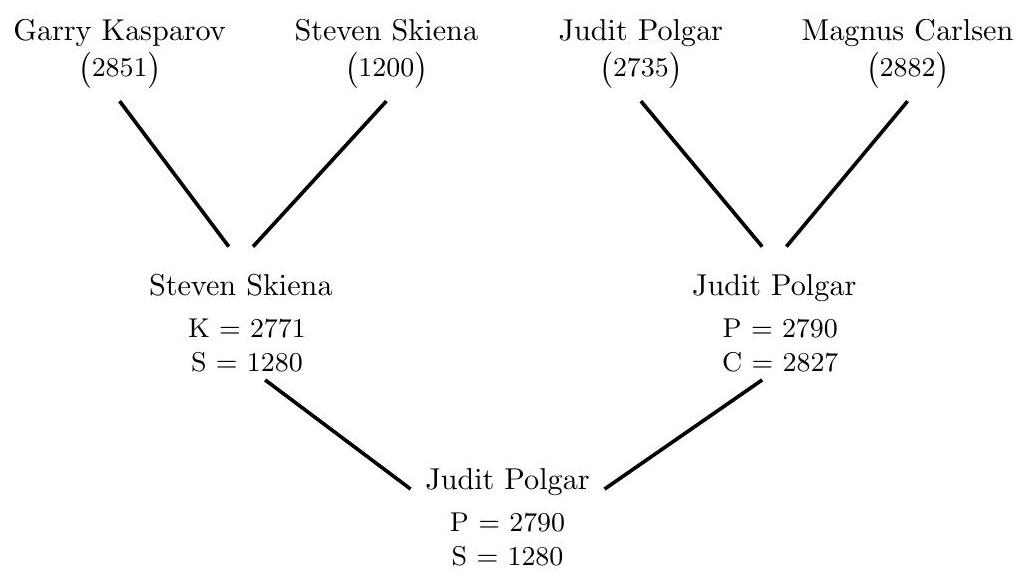
\includegraphics[max width=\textwidth]{2025_03_17_ca60ec0bfd96dcf8e028g-123}
\caption{Changes in ELO scores as a consequence of an unlikely chess tournament.}
\end{figure}

\begin{itemize}
  \item जब खिलाड़ी $B$ का बहुत बड़ा फ़ायदा होता है, $x \rightarrow -\infty$, और $f(-\infty) = 0$, इसका अर्थ होता है कि $B$ मैच जीतने के लिए पक्का है।
\end{itemize}

ये ठीक वही मान हैं जो हम चाहते हैं यदि $x$ खिलाड़ियों के बीच कौशल अंतर को मापता है।

लॉजिट फंक्शन इन ध्रुवों के बीच सहजता और सममिति से संक्रमण करता है। लॉजिट फंक्शन में पैरामीटर $c$ निर्धारित करता है कि परिवर्तन कितना तीव्र है। क्या कौशल में छोटे भेद जीतने की संभावना में बड़े भेद उत्पन्न करते हैं? जब$c = 0$ होता है, परिदृश्य पेनकेक जितना सपाट होता है: $f(x) = 1 / 2$ सभी$x$ के लिए। जब $c$ बड़ा होता है, तो परिवर्तन अधिक तीव्र हो जाता है, जैसा कि चित्र 4.5 में दिखाया गया है। वास्तव में, $c =\infty$ से एक स्टेप फंक्शन 0 से 1 तक उत्पन्न होता है।

$c = 1$को सेट करना एक उचित शुरुआत है, लेकिन सही चयन क्षेत्र विशिष्ट है। यह देखकर कि कितनी बार एक दिए गए कौशल-अंतर की मात्रा एक उलटफेर में परिणाम देती है (कमजोर पक्ष की जीत), इस पैरामीटर को निर्दिष्ट करने में मदद मिलती है। Elo शतरंज रैंकिंग प्रणाली को इस तरह से डिजाइन किया गया था कि$r(A) - r(B) = 400$का मतलब होता है कि$A$के पास जीतने की संभावना$B$से दस गुना अधिक है।

चित्र 4.6 Elo गणनाओं को दर्शाता है, एक अत्यंत असंभाव्य टूर्नामेंट के संदर्भ में जिसमें इतिहास के तीन महानतम शतरंज खिलाड़ी और एक निम्न-श्रेणी का खिलाड़ी शामिल है। यहाँ पर$k = 40$, जिसका अर्थ है कि किसी एकल मैच के परिणामस्वरूप अधिकतम संभव स्कोर में 80 अंकों का परिवर्तन हो सकता है। मानक लॉजिट फंक्शन ने कस्पारोव को पहले राउंड में स्कीना को हराने की 0.999886 संभावना दी, लेकिन लाजर को पुनर्जीवित करने जैसे चमत्कार के कारण मैच विपरीत दिशा में चला गया। इसके परिणामस्वरूप, 80 अंक कस्पारोव की रैंकिंग से मेरे खाते में चले गए।

दूसरी ओर कोष्ठक के परे दो वास्तविक शतरंज चैम्पियंस ने मुकाबला किया, जिसमें पोल्गर ने केवल 55 अंक बढ़ाकर अधिक कल्पनाशील अप्रत्याशित परिणाम किया। उसने अंतिम चरण में मुझे हरा दिया, एक उपलब्धि जो इतनी स्पष्ट रूप से अपेक्षित थी कि उसने मूल रूप से शून्य रेटिंग पॉइंट्स हासिल किए। इल्लो विधि जीत ही नहीं बल्कि आश्चर्यजनक परिणाम के जवाब में रेटिंग्स को अपडेट करने में बहुत प्रभावी है।

%---- Page End Break Here ---- Page : 107

\begin{center}
\begin{tabular}{l|cccll}
1 & A & B & A & A & $\mathrm{A}: 5$ \\
2 & C & A & B & B & $\mathrm{B}: 8$ \\\index{data!for evaluation}\index{data!for testing}\index{data!for training}\index{data formats!evaluation}
3 & B & C & C & D & $\mathrm{C}: 12$ \\
4 & D & D & E & C & $\mathrm{D}: 16$ \\
5 & E & E & D & E & $\mathrm{E}: 19$ \\
\end{tabular}
\end{center}

\textit{चित्र 4.7: बोर्डा की विधि का उपयोग करते हुए चार इनपुट रैंकिंग के सेट से $\{A, B, C, D, E\}$ की सहमति रैंकिंग का निर्माण करने के लिए, रैखिक भारों का उपयोग करके।}

\subsection{रैंकिंग का विलय}
कोई भी एकल संख्यात्मक विशेषता$f$, जैसे ऊँचाई, आइटम्स$n$के बीच युग्मwise तुलना$\binom{n}{2}$को उत्पन्न कर सकती है यह परीक्षण करके कि$f(A)>f(B)$प्रत्येक आइटम जोड़ी$A$और$B$के लिए। हम इन जोड़ों को इलो विधि में देकर एक रैंकिंग प्राप्त कर सकते हैं, लेकिन यह चीजों के बारे में सोचने का एक बेवकूफी भरा तरीका होगा। आखिरकार, इस तरह के किसी भी विश्लेषण का परिणाम केवल$f$के क्रमित क्रम को ही प्रतिबिंबित करेगा।

कई विभिन्न विशेषताओं द्वारा रैंकिंग के संग्रह को एकीकृत करना एक अधिक दिलचस्प समस्या बनाता है। यहाँ हम$i$\,वें विशेषता के क्रमबद्ध क्रम को रुचि के मदों पर एक क्रमचय$P_{i}$के रूप में परिभाषित करते हैं। हम सर्वसम्मति क्रमचय$P$की खोज करते हैं, जो किसी प्रकार सभी घटक क्रमचयों$P_{1},\ldots, P_{k}$को सर्वोत्तम रूप से प्रतिबिंबित करता है।

इसके लिए दो क्रमपरिवर्तनों के बीच समानता मापने के लिए एक दूरी फलन को परिभाषित करना आवश्यक है। एक समान समस्या स्पीयरमैन रैंक सहसंबंध गुणांक को परिभाषित करने में आई थी (देखें अनुभाग 2.3.1), जहाँ हमने तत्वों के सापेक्ष क्रम में सहमति के माप द्वारा दो चर की तुलना की थी।\footnote{ध्यान दें कि समानता माप और दूरी गणितीय का अंतर। सहसंबंध में, स्कोर बढ़ते हैं जब तत्व अधिक समान होते हैं, जबकि एक दूरी फलन में अंतर शून्य की ओर जाता है। दूरी गणितीय पर अधिक विस्तृत चर्चा अनुभाग 10.1.1 में की जाएगी।}

\textit{बोर्डा की विधि}एक साधारण स्कोरिंग प्रणाली का उपयोग करके कई अन्य रैंकिंग्स से एक सहमति रैंकिंग बनाती है। विशेष रूप से, हम क्रमचय में प्रत्येक के$n$स्थितियों को एक लागत या वजन सौंपते हैं। फिर, प्रत्येक$n$तत्वों के लिए, हम इसकी स्थितियों के भार को सभी$k$इनपुट रैंकिंग्स के ऊपर जोड़ते हैं। इन$n$स्कोर्स को क्रम में रखने से अंतिम सहमति रैंकिंग निर्धारित होती है।

अब केवल स्थिति और लागत के बीच मैपिंग स्पष्ट नहीं है। सबसे सरल लागत फ़ंक्शन प्रत्येक क्रम में$i$स्थान पर आने के लिए$i$अंक आवंटित करता है, अर्थात हम सभी क्रमों में तत्व के रैंक को जोड़ते हैं। यही हमने चित्र 4.7 के उदाहरण में किया है। वस्तु$A$को 3 बार पहले और 1 बार दूसरे स्थान पर आने के कारण$3\cdot1 + 1\cdot2 = 5$अंक मिलते हैं। वस्तु$C$को$2, 3, 3$, और 4 पर समाप्त होने के कारण 12 अंक मिलते हैं।$\{A, B, C, D, E\}$की अंतिम आम सहमति रैंकिंग सभी इनपुट रैंकिंग से सभी वोटों को एकीकृत करती है, हालांकि आम सहमति कम से कम भाग में सभी चार इनपुट रैंकिंग के साथ असहमत है।

लेकिन यह स्पष्ट नहीं है कि रेखीय वेट्स का उपयोग सबसे अच्छा विकल्प है क्योंकि यह मानता है कि तत्वों की स्थिति में हमारी सटीकता में समान विश्वास है।



आम तौर पर, हम अपनी शीर्ष पसंदों की विशेषताओं के बारे में सबसे अधिक जानेंगे, लेकिन हमारे पास उनके बीच के मध्य क्रम के बारे में स्पष्ट रूप से जानकारी नहीं होगी। अगर ऐसा है, तो एक बेहतर दृष्टिकोण यह हो सकता है कि 1st और 2nd के बीच के अंतर के लिए 110th और 111th के बीच की तुलना में अधिक अंक दिए जाएं।

इस प्रकार का भारण एक घंटी-आकार के वक्र द्वारा अंतर्निहित रूप से किया जाता है। मान लीजिए कि हम एक सामान्य वितरण से समान अंतराल पर $n$ वस्तुओं का नमूना लेते हैं, जैसा कि चित्र 4.8 में दिखाया गया है। इन $x$ मानों को स्थिति वाले भार के रूप में असाइन करना सबसे ऊँची और सबसे निचली रैंक पर केंद्र की तुलना में अधिक फैलाव उत्पन्न करता है। पूंछ वाले क्षेत्र वास्तव में उतने ही चौड़े होते हैं जितने ये 50 समान अंतराल वाले बिंदुओं के लिए दिखाई देते हैं: याद करें कि $95\%$ संभावना द्रव्यमान केंद्र के $2\sigma के भीतर स्थित होता है।

वैकल्पिक रूप से, अगर हमारा आत्मविश्वास समान नहीं है, तो हम आधा-सामान्य वितरण से नमूना ले सकते हैं, ताकि हमारे रैंक्स की पूंछ सामान्य वितरण के शिखर से भारित हो। इस तरह, सबसे ऊँची रैंक वाले तत्वों के बीच सबसे अधिक अंतर होता है, लेकिन पूंछ के तत्वों के बीच कम भेद होता है।

आपका यहाँ वेटिंग फंक्शन का चयन क्षेत्र-निर्भर होता है, इसलिए ऐसा चुनें जो आपके समस्या पर अच्छा कार्य करता प्रतीत होता है। सबसे\textit{उत्तम}कोस्ट फंक्शन की पहचान करना एक अपूर्ण समस्या बन जाता है। और विचित्र चीजें होती हैं जब हम आदर्श चुनाव प्रणाली बनाने का प्रयास करते हैं, जैसा कि सेक्शन 4.6 में दिखाया जाएगा।

\subsection{दिग्राफ-आधारित रैंकिंग}
\index{rankings!digraph-based}नेटवर्क एक समूह के मतों को सोचने का एक वैकल्पिक तरीका प्रदान करते हैं, जिसमें इस रूप में होता है कि "$A$ $B$ से आगे रैंक करता है।" हम एक निर्देशित ग्राफ/नेटवर्क का निर्माण कर सकते हैं जहाँ प्रत्येक इकाई के साथ एक शीर्ष बिंदु संबंधित होता है, और प्रत्येक मत के लिए निर्देशित किनारा $(A, B)$ होता है जिसमें $A$ $B$ से आगे रैंक करता है।

अनुकूलतम क्रमांकन तब उन शिखरों की एक क्रम व्यवस्थापन$P$ होगा जो...

%---- Page End Break Here ---- Page : 109

%---- Page End Break Here ---- Page : 109

\begin{figure}[H]
\centering
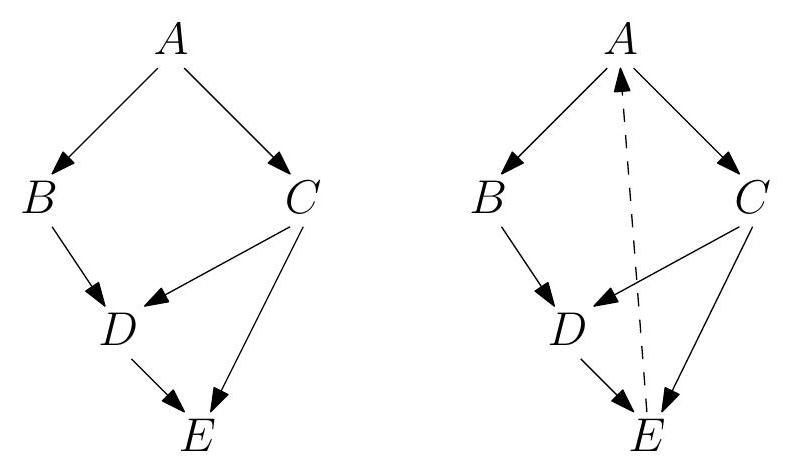
\includegraphics[max width=\textwidth]{2025_03_17_ca60ec0bfd96dcf8e028g-126}
\caption{Consistently ordered preferences yield an acyclic graph or DAG (left). Inconsistent preferences result in directed cycles, which can be broken by deleting small sets of carefully selected edges, here shown dashed (right).}
\end{figure}

एक निर्देशित ग्राफ जिसे चक्र नहीं होते हैं, उसे \textit{निर्देशित उभयनिष्ठ ग्राफ} या \textit{DAG} कहा जाता है। एक सतर्क पाठक जिसे एल्गोरिथम की थोड़ी पृष्ठभूमि होगी, याद करेगा कि इस श्रेष्ठतम शीर्षक क्रम को खोजने की प्रक्रिया को \textit{उभयनिष्ठ क्रम निर्धारण} कहा जाता है, जिसे रैखिक समय में कुशलता से किया जा सकता है। चित्र 4.9 (बाएं) एक DAG है, और इसके पास निर्देशित किनारों के अनुरूप ठीक दो भिन्न आदेश हैं: \textit{\{A, B, C, D, E\}} और \textit{\{A, C, B, D, E\}}।

लेकिन प्राकृतिक हीयूरिस्टिक्स होते हैं। जहाँ एक वर्टेक्स$v$का संबंध होता है, इसका एक अच्छा संकेतक इसका अंतर$d_{v}$है, जो उसके इन-डिग्री और आउट-डिग्री के बीच होता है। जब$d_{v}$अत्यधिक नकारात्मक होता है, तो यह संभवतः क्रम में आगे की ओर होगा, क्योंकि यह कई तत्वों पर प्रभुत्व रखता है लेकिन इस पर केवल कुछ तत्वों द्वारा प्रभुत्व होता है। एक अच्छा रैंकिंग क्रम बनाने के लिए इन अंतर के अनुसार वर्टेसेज़ को क्रम में रख सकते हैं। इससे भी बेहतर है कि सबसे नकारात्मक (या सबसे सकारात्मक) वर्टेक्स$v$को तर्कसंगत स्थान पर क्रमशः डालें, उस पर पड़ने वाली एजेज को हटाएँ, और फिर अगले सर्वश्रेष्ठ वर्टेक्स को स्थान देने से पहले गणनाओं को समायोजित करें।\index{Feynman, Richard}\index{modeling!simulation}\index{monotonic!simulations}

\section{पेजरैन्क}
\index{PageRank}नेटवर्क में शीर्यकणों को उनकी महत्वता के अनुसार क्रमबद्ध करने का एक और अधिक प्रसिद्ध तरीका है: Google's सर्च इंजन के आधारभूत \textbf{पेजरैन्क}एल्गोरिद्म।

वेब वेबपृष्ठों से निर्मित होता है, जिनमें से अधिकांश में अन्य वेबपृष्ठों के लिंक होते हैं। आपका वेबपृष्ठ मेरे वेबपृष्ठ से लिंक करता है, यह एक प्रच्छन्न समर्थन है कि आप सोचते हैं कि मेरा पृष्ठ काफी अच्छा है। यदि इसे इस रूप में व्याख्यायित किया जाए कि "आप सोचते हैं मेरा पृष्ठ आपके पृष्ठ से बेहतर है", तो हम लिंक नेटवर्क का निर्माण कर सकते हैं और इसे अधिकतम ऐसिक्लिक-उपग्राफ से संबोधित समस्या के रूप में देख सकते हैं, जैसा कि पिछले उपवर्ग में चर्चा की गई थी।

लेकिन प्रभुत्व वास्तव में वेब पर लिंक के लिए सही व्याख्या नहीं है। पेजरैंक इसके बजाय उन वर्टिसेज़ को पुरस्कृत करता है जिनके पास सबसे अधिक इन-लिंक्स हैं: यदि सभी रास्ते रोम को जाते हैं, तो रोम निश्चित रूप से एक काफी महत्वपूर्ण स्थान होना चाहिए। इसके अलावा, यह इन-लिंक्स को स्रोत की ताकत से मापता है: एक महत्वपूर्ण पेज से मेरे लिए लिंक का मूल्य स्पैम साइट से एक लिंक से अधिक होना चाहिए।

\section{युद्ध कहानी: क्लाइड का प्रतिशोध}
\index{Clyde}हाई स्कूल के मेरे सोफोमोर वर्ष के दौरान, मेरे मन में पेशेवर फुटबॉल खेलों के परिणाम की भविष्यवाणी करने के लिए एक प्रोग्राम लिखने का विचार आया। मुझे खेल के रूप में फुटबॉल में विशेष रुचि नहीं थी, लेकिन मैंने देखा कि मेरे कई सहपाठी सप्ताहांत फुटबॉल खेलों के परिणाम पर अपने दोपहर के भोजन के पैसे की शर्त लगा रहे थे। मेरे लिए यह स्पष्ट था कि एक ऐसा प्रोग्राम लिखना जो फुटबॉल खेलों के परिणाम को सटीकता से भविष्यवाणी कर सके, उसका बड़ा मूल्य हो सकता है, और इसके अलावा यह करने के लिए एक बहुत ही रोमांचक काम हो सकता है।

पिछली दृष्टि में, वह प्रोग्राम जो मैंने तैयार किया था अब अत्यधिक कच्चा प्रतीत होता है। मेरा प्रोग्राम टीम$x$द्वारा बनाए गए अंकों और टीम$y$द्वारा स्वीकार किए गए अंकों के औसत का उपयोग करता था भविष्यवाणी करने के लिए कि टीम$x$टीम$y$के खिलाफ कितने अंक प्राप्त करेगी।

\begin{equation}
\begin{aligned}
P_{x} &= \frac{((\text{points scored by team } x) + (\text{points allowed by team } y))}{2 \times (\text{games played})} \\
P_{y} &= \frac{((\text{points scored by team } y) + (\text{points allowed by team } x))}{2 \times (\text{games played})}
\end{aligned}
\end{equation}

यह कंप्यूटर प्रोग्राम,\textit{क्लाइड}, वास्तविक दुनिया के किसी पहलू के लिए एक स्कोरिंग फ़ंक्शन बनाने का मेरा पहला प्रयास था। इसमें तर्क की एक निश्चित मात्रा कारगर हो रही थी। अच्छी टीमों का स्कोर उनसे ज्यादा होता है जितना वे अनुमति देते हैं, जबकि बुरी टीमों को उनसे ज्यादा अंक मिलते हैं जितना वे स्कोर कर पाते हैं। यदि टीम$x$एक टीम$y$के खिलाफ खेलती है जिसने बहुत सारे अंक छोड़े हैं, तो$x$को$y$के खिलाफ अधिक अंक स्कोर करने चाहिए जितना कि वह एक और टीम के खिलाफ करेगी जिसमें अधिक ताकतवर रक्षा है।

%---- Page End Break Here ---- Page : 111

टीमों की सुरक्षा बेहतर होती है। इसी तरह, जितने अधिक अंक टीम$x$ने बाकी लीग के खिलाफ हासिल किए हैं, उतने ही अधिक अंक यह$y$के खिलाफ प्राप्त करने की संभावना है।

बिल्कुल, यह साधारण मॉडल फुटबॉल वास्तविकता के सभी पहलुओं को नहीं दर्शा सकता। मान लीजिए कि टीम$x$अब तक के सीजन में सभी कमजोर टीमों के साथ खेल रही है, जबकि टीम$y$लीग में सबसे बेहतरीन टीमों के खिलाफ खेल रही है। टीम$y$टीम$x$से बहुत बेहतर हो सकती है, भले ही उसके रिकॉर्ड अब तक खराब हों। यह मॉडल उन चोटों की भी अनदेखी करता है जिनसे कोई टीम जूझ रही हो सकती है, मौसम गर्म है या ठंडा, और क्या टीम अपने खेल में गर्म है या ठंडी। यह उन सभी कारकों को नजरअंदाज करता है जो खेलों को स्वाभाविक रूप से अप्रत्याशित बनाते हैं।

और फिर भी, इस तरह का सरल मॉडल फुटबॉल खेलों के परिणाम की भविष्यवाणी करने में एक उचित काम कर सकता है। यदि आप उपरोक्त तरह से पॉइंट एवरेज की गणना करते हैं, और घरेलू टीम को तीन अतिरिक्त अंक बोनस के रूप में देते हैं, तो आप लगभग दो-तिहाई फुटबॉल खेलों के विजेता का चयन करेंगे। इसकी तुलना उस और भी अधिक अनुकरणशील मॉडल से करें जो केवल सिक्का उछाल कर करता है, जो केवल आधे खेलों की सही भविष्यवाणी करता है। यह पहला बड़ा सबक था जो क्लाइड ने मुझे सिखाया:

\textit{यहां तक कि साधारण गणितीय मॉडल भी वास्तविक भविष्यवाणी शक्ति रख सकते हैं।}
\index{Mathematica}
एक साहसी 16 वर्ष के किशोर के रूप में, मैंने हमारे स्थानीय समाचार पत्र, \textit{द न्यू ब्रंसविक होम न्यूज} को लिखा, यह बताते हुए कि मेरे पास फुटबॉल खेलों के परिणामों की भविष्यवाणी के लिए एक कंप्यूटर प्रोग्राम है और मैं उन्हें हर सप्ताह मेरे भविष्यवाणियों को प्रकाशित करने का विशेष अवसर देने के लिए तैयार था। याद करें कि यह 1977 में था, जब व्यक्तिगत कंप्यूटर ने सार्वजनिक चेतना में प्रवेश नहीं किया था। उन दिनों में, वास्तव में एक हाई स्कूल के बच्चे का \textit{कंप्यूटर का उपयोग} करना काफी आश्चर्यजनक नवीनता की बात थी। यह समझने के लिए कि समय कितना बदल गया है, अखबार द्वारा कलाईड और मेरे बारे में प्रकाशित आलेख को चित्र 4.10 में देखें।

मुझे नौकरी मिल गई। क्लाइड ने 1977 नेशनल फुटबॉल लीग के प्रत्येक खेल के परिणाम की भविष्यवाणी की। जैसा कि मुझे याद है, क्लाइड और मैंने सत्र का समापन 135-70 के प्रतीत होने वाले प्रभावशाली रिकॉर्ड के साथ किया। प्रत्येक सप्ताह, वे मेरी भविष्यवाणियों की तुलना अखबार के खेल लेखकों की भविष्यवाणियों से करते थे। जैसा कि मुझे याद है, हम सभी एक-दूसरे से कुछ ही खेलों के भीतर समाप्त हुए, यद्यपि अधिकांश खेल लेखक कंप्यूटर से बेहतर रिकॉर्ड के साथ समाप्त हुए।

\textit{होम न्यूज़}मेरे काम से इतना प्रभावित हुआ कि उन्होंने मुझे अगले सीजन के लिए नवीनीकृत नहीं किया। हालांकि, 1978 सीजन के लिए क्लाइड की पसंदें \textit{फिलाडेल्फिया इन्क्वायरर} में प्रकाशित हुईं, जो एक बहुत बड़ा अखबार था। हालांकि, मेरे पास यह कॉलम अकेले नहीं था। इसके बजाय, \textit{इन्क्वायरर} ने मुझे दस शौकिया और पेशेवर भविष्यवक्ताओं, या टाउट्स के बीच शामिल किया। हर हफ्ते हमें पॉइंट स्प्रेड के खिलाफ चार खेलों के परिणामों की भविष्यवाणी करनी होती थी।

फुटबॉल में प्वाइंट स्प्रेड एक तरीका है जिससे मजबूत टीमों को सट्टेबाजी के उद्देश्य से हैंडीकैप किया जाता है। प्वाइंट स्प्रेड को इस तरह से डिज़ाइन किया गया है कि हर खेल को 50/50 प्रस्ताव बनाकर प्रस्तुत किया जाए, और इसलिए यह खेलों के परिणाम की भविष्यवाणी करना बहुत कठिन बना देता है।

क्लाइड और मैंने 1978 के नेशनल फुटबॉल लीग सीज़न के दौरान फैलाव के खिलाफ बहुत अच्छा नहीं किया, और ज्यादातर अन्य \textit{फिलाडेल्फिया इंक्वायरर}तौट्स ने भी नहीं किया। हमने केवल 46\% खेलों की सही भविष्यवाणी की, जो कि दस प्रकाशित प्रॉग्नॉस्टिकेटर्स में से 7वें स्थान पर खत्म करने के लिए पर्याप्त (या खराब) प्रदर्शन था। फैलाव के खिलाफ चुनने से मुझे जीवन का दूसरा महत्वपूर्ण सबक मिला:

\section{मृवन्ट कंप्यूटरों का उपयोग फुटबॉल विजेताओं की भविष्यवाणी करने के लिए करता है}
\index{football}ईस्ट ब्रुन्सविक - ईस्ट ब्रुन्सविक हाई स्कूल का एक 16 वर्षीय छात्र ने फुटबॉल में रुचि को कंप्यूटर के प्रति आकर्षण के साथ जोड़ने का तरीका खोज लिया है।

स्टीवन स्कीना कहते हैं कि वह मुकाबला करने वाली टीमों के बारे में संबंधित जानकारी एक कंप्यूटर में डालकर पेशेवर फुटबॉल खेलों के परिणाम को उच्च सटीकता के साथ निर्धारित कर सकते हैं।

"विजेता लगभग हमेशा सही होते हैं," 5 क्यूरियर रोड, डन्हाम्स कॉर्नर रोड पर रहने वाले हाई स्कूल जूनियर ने कहा। "जब मैंने पिछले सीजन के अंत में भविष्यवाणी करना शुरू किया, तो मेरे पास 85 प्रतिशत सटीकता दर थी।"

वह इसे टीम रिकॉर्ड्स, स्कोर और अनुमति दिए गए पॉइंट्स, खेल के दौरान प्राप्त और अनुमति दिए गए औसत गज, रशिंग और पासिंग श्रेणियों में विभाजित प्राप्त और अनुमति दिए गए गज की विस्तृत जानकारी, घर और बाहर के प्रदर्शन, और भी कई अन्य आंकड़ों को कंप्यूटर में डालकर करता है।

जानकारी फुटबॉल सांख्यिकी और स्टैंडिंग की साप्ताहिक संकलन से एकत्र की जाती है। स्कीना तथ्यों को इंडेक्स कार्ड्स पर लिखते हैं और फिर उन्हें हाई स्कूल के छह कंप्यूटर टर्मिनल्स में से एक या ⸨लाइब्रेरी⸩ में एक टर्मिनल में टाइप करते हैं जहाँ वह स्कूल के बाद अंशकालिक काम करते हैं।

"मुझे एक जीतने वाली टीम मिलती है, प्रत्येक टीम के लिए एक दशमलव स्कोर और एक प्वाइंट स्प्रेड," उस किशोर ने कहा जिसने पिछले साल हाई स्कूल में कम्प्यूटर प्रोग्रामिंग कोर्स पूरा किया था।

उसका पहला प्रयास जीतने वालों का चयन करने के लिए सोमवार रात के खेल में था, जिसमें ओकलैंड रेडर्स, जो अंतिम सुपर बाउल विजेता बने, और सिनसिनाटी बंगाल्स शामिल थे।

यह विश्लेषण करने के लिए एक कठिन खेल था क्योंकि सिनसिनाटी एक प्लेऑफ़ स्थान के लिए लड़ रहा था जबकि ओकलैंड पहले ही पोस्ट-सीज़न प्रतियोगिता में स्थान सुरक्षित कर चुका था।

"कोई नहीं जानता था कि ऑकलैंड १०० प्रतिशत दे रहा है या नहीं," स्कीना ने कहा। "लेकिन मेरी गणनाएँ दिखा रही थीं कि वे २४-२० से जीतेंगे। अंतिम स्कोर ३५-२० था। उन्होंने पूरी ताकत से खेला।"

स्कीना ने कहा कि उन्होंने अगले सप्ताह 14 में से 12 विजेताओं को चुना और सटीक रूप से भविष्यवाणी की कि ओकलैंड मिनेसोटा को सुपर बाउल में हराएगा।

नेशनल फुटबॉल लीग की 1778 रिकॉर्ड बुक, जो लीग की 28 टीमों के पिछले साल की आँकड़ों को विभाजित करती है, स्कीना की जानकारी के लिए 1977 सत्र के पहले कुछ हफ्तों के लिए मुहैया कराएगी। वह इस साल प्रत्येक टीम द्वारा खेले गए अंतिम दो प्रदर्शनी मैचों के आँकड़ों का भी उपयोग करेगा।

स्कीना ने एक कंप्यूटर प्रोग्राम लिखा जो 17 सांख्यिकी चर पर आधारित था जो एक फुटबॉल खेल के दौरान आ सकते थे।

कम्प्यूटर, मूल रूप से, उससे प्रश्न पूछता है और वह उत्तर टाइप करता है।

"यह टीमों के नाम पूछकर शुरू होता है," उसने कहा। "फिर यह रिकॉर्ड्स, स्कोर किए गए पॉइंट्स, आदि पूछेगा..."

कंप्यूटर प्रोग्राम में चोटों जैसे अमूर्त चर शामिल करने का प्रयास भी किया जाता है।

"चोटें आक्रमण, रक्षा, और क्वार्टरबैक में विभाजित होती हैं," उन्होंने समझाया। "जाहिर है कि क्वार्टरबैक की चोट सबसे गंभीर होती है। प्रत्येक स्थिति के लिए चोटों को विभाजित करना बहुत कठिन है। जब कंप्यूटर रक्षा पर चोटों की संख्या पूछता है, तो मैं एक, दो या जो भी संख्या हो, वह टाइप करता हूँ।"

क्या विल स्किने अपनी कम्प्यूटर ग़णनाओं का उपयोग सीज़न के दौरान उपलब्ध फुटबॉल पूल्स और प्रतियोगिताओं में भाग लेने के लिए करेंगे?

"नहीं," उसने कहा। "मुझे अपनी भविष्यवाणियों पर सट्टा लगाना पसंद नहीं है। पिछले सीजन में एक दोस्त ने एक खेल पर सट्टा लगाया जिसकी मैंने भविष्यवाणी की थी और यह उन कुछ में से एक निकला⸨ जो ⸩

\begin{figure}[h]
    \centering
    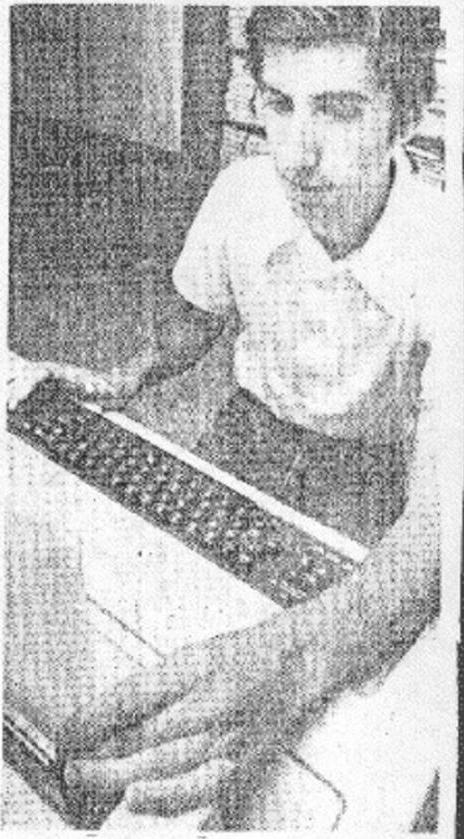
\includegraphics[max width=\textwidth]{2025_03_17_ca60ec0bfd96dcf8e028g-129}
    \caption{My first attempt at mathematical modeling.}
    \label{fig:first_att_modeling}
\end{figure}

\textbf{\textit{स्टीवन स्कीना}}

...उनकी सटीकता का परीक्षण करने के लिए\index{data}\index{linear algebra}\index{linear algebra!power of}\index{matrix}\index{Rota, Gian-Carlo}

\section{प्रेडिक्शन्स प्रकाशित}
स्टीवन स्कीना को \textit{द होम न्यूज़} में प्रत्येक रविवार को पेशेवर फुटबॉल प्रोग्नॉस्टिकेटर के रूप में अपनी कौशल दिखाने का अवसर मिलेगा।

होम न्यूज़ के कार्यकारी संपादक रॉबर्ट ई. रोड्स के अनुसार युवा के साप्ताहिक चयन हमारे फुटबॉल कवरेज में "एक अतिरिक्त तत्व" होंगे।

"मुझे लगता है कि यह हमारे लिए इसे आज़माने के लिए काफ़ी दिलचस्प है," रोड्स ने किशोर के कंप्यूटर मेथड के बारे में कहा कि कैसे खेलों के परिणाम का निर्धारण किया जाए। वह एक ईमानदार युवा व्यक्ति लगता है और हम उसके साथ खड़े रहेंगे।"

स्कीना जीतने वालों की भविष्यवाणी करने, प्रत्येक टीम के लिए स्कोर बताने और अपनी निष्कर्ष के कारणों को संक्षेप में समझाने के लिए एक "मामूली मानदेय" प्राप्त करेंगे।

उनका कॉलम पहली बार रविवार के खेल सेक्शन में दिखाई देगा जब नेशनल फुटबॉल लीग (एएफएल) अपनी 1977 की सीज़न की शुरुआत 13 खेलों के साथ करेगी। स्कीना लीग के सोमवार रात के खेलों के नतीजों की भी भविष्यवाणी करेंगे।

द\textit{मुख्य समाचार}खेल अनुभाग में इस स्तंभ को प्रकाशित कर रहा है ताकि युवाओं की प्रणाली का परीक्षण किया जा सके और फुटबॉल प्रेमियों को एक मनोरंजक विशेषता प्रदान की जा सके। इसका उद्देश्य सट्टेबाजी को प्रोत्साहित करना नहीं है। "हम खेल के समय के काफी करीब उनकी पसंद को छापेंगे ताकि सट्टेबाजी को रोका जा सके," रोड्स ने कहा। "पेशेवर फुटबॉल में बड़ी दिलचस्पी है और सबसे बढ़कर, हम उसकी प्रणाली का परीक्षण करना चाहते हैं। मैं उसके लिए समर्थन करूँगा।"

\section{ऐरो का असंभवता प्रमेय}
हमने डेटा से रैंकिंग या स्कोरिंग फ़ंक्शन बनाने के लिए कई विधियाँ देखी हैं। यदि हमारे पास कुछ संस्थाओं के लिए "सही" सापेक्ष क्रम की एक स्वर्ण मानक रिपोर्ट है, तो इसे हमारे स्कोरिंग फ़ंक्शन को प्रशिक्षित या मूल्यांकित करने के लिए उपयोग किया जा सकता है ताकि यह इन रैंकिंग के साथ अधिकतम सीमा तक सहमति करे।

लेकिन बिना किसी सोने के मानक के, यह दिखाया जा सकता है कि कोई सर्वश्रेष्ठ रैंकिंग प्रणाली मौजूद नहीं है। यह \textit{एरो का असंभाव्यता प्रमेय} का परिणाम है, जो साबित करता है कि वरीयताओं के क्रम को एकत्र करने के लिए कोई भी चुनाव प्रणाली निम्नलिखित वांछनीय और निर्दोष गुणों को संतुष्ट नहीं कर सकती:

\begin{itemize}यह प्रणाली पूर्ण होनी चाहिए, जिसमें जब \itemA$ और $B$ वैकल्पिक विकल्पों के बीच चुनने को कहा जाए, तो यह कहे (1) $A$ को $B$ से अधिक पसंद किया जाता है, (2) $B$ को $A$ से अधिक पसंद किया जाता है, या (3) दोनों के बीच समान पसंद है।
\end{itemize}

%---- Page End Break Here ---- Page : 114
% Mismatched: \subsectionname{War Story: Who's Bigger?}
My students sometimes tell me that I am history. I hope this isn't true quite yet, but I am very interested in history, as is my former postdoc Charles Ward. Charles and I got to chatting about who the most significant figures in history were, and how you might measure this. Like most people, we found our answers in Wikipedia.

विकिपीडिया एक अद्भुत चीज़ है, जो 100,000 से अधिक लेखकों द्वारा निर्मित एक वितरित कार्य उत्पाद है, जो किसी तरह से सामान्य रूप से सही और गहराई का मानक बनाए रखता है। विकिपीडिया मानव ज्ञान की एक आश्चर्यजनक मात्रा को एक खुले और मशीन द्वारा पढ़ने योग्य रूप में संगृहीत करता है।

हमने ऐतिहासिक रैंकिंग के आधार के रूप में डेटा स्रोत के रूप में इंग्लिश विकिपीडिया का उपयोग करने का निर्णय लिया। हमारा पहला कदम प्रत्येक व्यक्ति के विकिपीडिया पृष्ठ से फ़ीचर वेरिएबल्स को निकालना था जो स्पष्ट रूप से ऐतिहासिक महत्व से संबंधित होने चाहिए। इसमें निम्नलिखित विशेषताएँ शामिल थीं:

\begin{itemize}
  \item \textit{लंबाई:} सबसे महत्वपूर्ण ऐतिहासिक व्यक्तियों के विकिपीडिया पृष्ठ सामान्य लोगों की तुलना में अधिक लंबे होने चाहिए। इसलिए, शब्दों में लेख की लंबाई कुछ हद तक ऐतिहासिक महत्त्व को दर्शाने वाली एक प्राकृतिक विशेषता प्रदान करती है।\index{geometry}\index{vectors}\index{vectors!unit}
  \item \textit{हिट्स:} सबसे महत्वपूर्ण व्यक्ति के विकिपीडिया पृष्ठ अन्य लोगों की तुलना में अधिक बार पढ़े जाते हैं, क्योंकि वे अधिक लोगों के लिए अधिक रुचिकर होते हैं। मेरा विकिपीडिया पृष्ठ प्रतिदिन औसतन बीस बार देखा जाता है, जो कि काफ़ी बढ़िया है। लेकिन आइज़क न्यूटन का पृष्ठ प्रतिदिन औसतन 7700 बार देखा जाता है, जो कि बहुत अच्छा है।
  \item \textit{पेजरैंक:} महत्वपूर्ण ऐतिहासिक व्यक्ति अन्य महत्वपूर्ण ऐतिहासिक व्यक्तियों के साथ परस्पर संपर्क करते हैं, जो विकिपीडिया लेखों में हाइपरलिंक संदर्भों के रूप में परिलक्षित होते हैं। यह एक निर्दिष्ट ग्राफ़ को परिभाषित करता है जहां शीर्ष लेख होते हैं और निर्दिष्ट किनारों के रूप में हाइपरलिंक्स होते हैं। इस ग्राफ़ का पेजरैंक गणना करने से प्रत्येक ऐतिहासिक व्यक्ति की केंद्रीयता मापी जाएगी, जो महत्व के साथ अच्छी तरह से मेल खाती है।
\end{itemize}

कुल मिलाकर, हमने प्रत्येक ऐतिहासिक व्यक्ति के लिए छह विशेषताएँ निकालीं। अगले चरण में, हमने इन चर को सामान्यीकृत किया, मुख्य रूप से मूल रैंकिंग को सामान्य रूप से वितरित वज़न के साथ संयोजित करके, जैसा कि अनुभाग 4.4.2 में सुझाया गया था। हमने\textit{सांख्यिकीय कारक विश्लेषण}नामक एक तकनीक का उपयोग किया, जो प्रिंसिपल कंपोनेंट विश्लेषण से संबंधित है (जिस पर चर्चा अनुभाग 8.5.2 में की गई है), जिससे हमने दो कारकों को अलग-थलग किया जो हमारे डेटा में अधिकांश विचरण को समझाते हैं। इन चर के एक साधारण रेखीय संयोजन से हमें एक स्कोरिंग फ़ंक्शन मिला, और हमने अपने प्रारंभिक रैंकिंग का निर्धारण करने के लिए स्कोर को क्रमबद्ध किया, जिसका हमने नाम\textit{प्रसिद्धि} रखा।

हमारी प्रसिद्धि स्कोर के आधार पर शीर्ष बीस आंकड़े चित्र 4.12 (दाईं ओर) में दिखाए गए हैं। हमने इन रैंकिंग का अध्ययन किया और निर्णय लिया कि यह वास्तव में वह नहीं दर्शा रहा था जो हम चाहते थे। प्रसिद्धि के आधार पर शीर्ष बीस में पॉप संगीतकार जैसे मैडोना और माइकेल जैक्सन, और तीन समकालीन अमेरिकी राष्ट्रपति शामिल थे। यह स्पष्ट था कि समकालीन व्यक्ति हमारे सोच से कहीं अधिक ऊंचे स्थान पर थे: हमारी स्कोरिंग कार्यप्रणाली वर्तमान प्रसिद्धि को ऐतिहासिक महत्ता की तुलना में अधिक पकड़ रही थी।

हमारा समाधान समकालीन व्यक्तियों के स्कोर को समय के अनुसार घटाने का था। यह प्रभावशाली है कि वर्तमान में एक सेलिब्रिटी को विकिपीडिया पर बहुत अधिक हिट्स मिलते हैं, लेकिन यह अधिक प्रभावशाली है कि हम अभी भी 300 वर्ष पहले मरे किसी व्यक्ति के बारे में परवाह करते हैं। आयु-सुधार के बाद शीर्ष बीस व्यक्तियों को चित्र 4.12 (बाएं) में दिखाया गया है।

\begin{center}
\begin{tabular}{c|ccc}
Voter & Red & Green & Blue \\
\hline
x & 1 & 2 & 3 \\
y & 2 & 3 & 1 \\\index{Lincoln, Abraham}\index{matrix!addition}\index{matrix!linear combinations of}\index{matrix!transpose of}\index{sampling!multiplication}
z & 3 & 1 & 2 \\
\hline
\end{tabular}
\end{center}

चित्र 4.11: रंगों के लिए पसंद की रैंकिंग जो पारगमनता के नुकसान को दर्शाती है। लाल को हरे से अधिक पसंद किया जाता है और हरे को नीले से, फिर भी नीला लाल से अधिक पसंद किया जाता है।

\begin{itemize}
  \item परिणाम संक्रमणशील होने चाहिए, जिसका अर्थ है कि यदि $A$ को $B$ से अधिक पसंद किया जाता है, और $B$ को $C$ से अधिक पसंद किया जाता है, तो $A$ को $C$ से अधिक पसंद किया जाना चाहिए।
  \item यदि हर व्यक्ति $A$ को $B$ से अधिक पसंद करता है, तो प्रणाली को $A$ को $B$ से अधिक पसंद करना चाहिए।
  \item प्रणाली को केवल एक व्यक्ति, एक तानाशाह की पसंद पर निर्भर नहीं होना चाहिए।
  \item $A$ की $B$ की तुलना में पसंद किसी अन्य विकल्प, जैसे $C$ की पसंद से स्वतंत्र होनी चाहिए।
\end{itemize}

चित्र 4.11 ऐरो के प्रमेय का कुछ स्वाद और "रॉक-पेपर-सीज़र्स" प्रकार की गैर-परिवर्ती आर्डरिंग की प्रकृति को दर्शाता है। यह तीन मतदाताओं ($x, y$, और$z$) के रंगों के बीच उनकी प्राथमिकताओं को रैंक करता है। दो रंगों$a$और$b$के बीच प्राथमिकता स्थापित करने के लिए, एक तार्किक प्रणाली यह तुलना कर सकती है कि कितने क्रम $a$को$b$से पहले और$b$को$a$से पहले रैंक करते हैं। इस प्रणाली के अनुसार, लाल को हरा रंग से$x$और$y$द्वारा प्राथमिकता दी जाती है, इसलिए लाल जीतता है। इसी प्रकार, हरे को नीले से$x$और$z$द्वारा प्राथमिकता दी जाती है, इसलिए हरा जीतता है। संक्रमणीयता के अनुसार, लाल को इन परिणामों के अनुसरण के रूप में नीले पर अवश्य प्राथमिकता दी जानी चाहिए। फिर भी$y$और$z$नीले को लाल पर प्राथमिकता देते हैं, जो इस गुण का उल्लंघन करता है जिसे हम चाहते हैं कि हमारी चुनाव प्रणाली बनाए रखे।

एरो का प्रमेय बहुत आश्चर्यजनक है, लेकिन क्या इसका मतलब है कि हमें डेटा का विश्लेषण करने के लिए रैंकिंग को एक उपकरण के रूप में छोड़ देना चाहिए? बिलकुल नहीं, जैसे एरो का प्रमेय नहीं चाहता कि हम लोकतंत्र को छोड़ दें। बहुसंख्यकों के नियम के विचार पर आधारित पारंपरिक मतदान प्रणालियाँ आमतौर पर लोकप्रिय प्राथमिकताओं को दर्शाने का अच्छा काम करती हैं, विशेषकर जब इन्हें बड़ी संख्या में उम्मीदवारों से निपटने के लिए उपयुक्त रूप से सामान्यीकृत किया जाता है। और इस अध्याय की तकनीकें आमतौर पर वस्तुओं को दिलचस्प और अर्थपूर्ण तरीकों से रैंक करने का अच्छा काम करती हैं।

\textit{घर पर सीखने का पाठ:}हम सही रैंकिंग नहीं खोजते हैं, क्योंकि यह एक स्पष्ट रूप से परिभाषित उद्देश्य नहीं है। इसकी बजाय, हम ऐसी रैंकिंग खोजते हैं जो उपयोगी और दिलचस्प हों।
%---- पृष्ठ समाप्ति विराम यहाँ ---- पृष्ठ : 116

\begin{center}
\begin{tabular}{|r|l|c|l|}\index{associativity}\index{matrix multiplication!applications}
\hline
Signif & \multicolumn{1}{|c|}{Name} & \multicolumn{1}{|c|}{Fame} & \multicolumn{1}{|c|}{Person} \\
\hline
1 & Jesus & 1 & George W. Bush \\
2 & Napoleon &  &  \\
3 & William Shakespeare & 2 & Barack Obama \\
4 & Muhammad & 3 & Jesus \\
5 & Abraham Lincoln & 4 & Adolf Hitler \\
6 & George Washington & 5 & Ronald Reagan \\
7 & Adolf Hitler & 6 & Bill Clinton \\
8 & Aristotle & 7 & Napoleon \\
9 & Alexander the Great &  &  \\
10 & Thomas Jefferson & 8 & Michael Jackson \\
11 & Henry VIII & 9 & W. Shakespeare \\
12 & Elizabeth I & 10 & Elvis Presley \\
13 & Julius Caesar & 11 & Muhammad \\
14 & Charles Darwin & 12 & Joseph Stalin \\
15 & Karl Marx & 13 & Abraham Lincoln \\
16 & Martin Luther & 14 & G. Washington \\
17 & Queen Victoria & 15 & Albert Einstein \\
18 & Joseph Stalin & 16 & John F. Kennedy \\
19 & Theodore Roosevelt &  &  \\
20 & Albert Einstein & 17 & Elizabeth II \\
 & 18 & John Paul II &  \\
 & 19 & Madonna &  \\
20 & Britney Spears &  &  \\
\hline
\end{tabular}
\end{center}

\begin{figure}[h]
\caption{The top 20 historical figures, ranked by significance (left) and contemporary fame (right).}
\end{figure}

अब\textit{यही}वह था जिसकी हम तलाश कर रहे थे! हमने रैंकिंग्स को इतिहासिक महत्व के लिए मिल सकने वाले प्रो़़क्सी का उपयोग करके सत्यापित किया: अन्य प्रकाशित रैंकिंग्स, हस्ताक्षर कीमतें, खेल आँकड़े, इतिहास की पाठ्यपुस्तकें, और प्रसिद्धि के हॉल चुनाव परिणाम। हमारी रैंकिंग्स ने इन सभी प्रो़़क्सी के खिलाफ एक मजबूत सहसंबंध दिखाया।

वास्तव में, मैं सोचता हूँ कि ये रैंकिंग्स बहुत ही शानदार तरीके से जानकारीपूर्ण हैं। हमने एक बुक लिखी है जो उन सभी प्रकार की चीज़ों का वर्णन करती है जो उनसे सीखी जा सकती हैं \cite{SW13}। मैं गर्व से आपको इसे पढ़ने के लिए प्रोत्साहित करता हूँ यदि आप इतिहास और संस्कृति में रुचि रखते हैं। जितना अधिक हमने इन रैंकिंग्स का अध्ययन किया, उतना ही मैं उनकी सामान्य समझदारी पर प्रभावित हुआ।

हालाँकि, हमारे प्रकाशित रैंकिंग्स का सार्वभौमिक सहमति से मिलना नहीं हुआ। इससे बहुत दूर। दर्जनों ⸨newspaper⸩ और ⸨magazine⸩ लेख हमारे रैंकिंग्स के बारे में प्रकाशित हुए, कई बहुत विरोधी थे। लोगों ने उन्हें सम्मान क्यों नहीं दिया, हमारे व्यापक प्रमाणीकरण के बावजूद? पिछली ओर देखते हुए, अधिकांश आलोचना जो हमने झेली, तीन भिन्न कारणों से आई:

\begin{itemize}
\item \textit{विभिन्न अंतर्निहित महत्व की धारणाएं:} हमारी विधियों को \textit{मेम-शक्ति} मापने के लिए डिज़ाइन किया गया था, कि ये ऐतिहासिक हस्तियां अपने नामों को इतिहास में कितनी सफलतापूर्वक प्रचारित कर रही थीं। लेकिन कई पाठकों का मानना था कि हमारी विधियों को ऐतिहासिक \textit{महानता} की धारणाओं को पकड़ना चाहिए। कौन सबसे महत्वपूर्ण था, दुनिया को बदलने के संदर्भ में? और क्या हम दुनिया को या सिर्फ अंग्रेज़ी बोलने वाली दुनिया को मतलब रखते हैं? जब वे दुनिया की आबादी के $30 \%$ से अधिक का प्रतिनिधित्व करते हैं, तो इस सूची में कोई चीनी या भारतीय व्यक्ति कैसे नहीं हो सकता?\\
हमें मापने से पहले इस बात पर सहमत होना चाहिए कि हम क्या मापने की कोशिश कर रहे हैं। ऊँचाई आकार का एक उत्कृष्ट उपाय है, लेकिन यह मोटेपन को पकड़ने का अच्छा काम नहीं करता है। हालांकि, एक बास्केटबॉल टीम के लिए खिलाड़ियों का चयन करने के लिए ऊँचाई बहुत उपयोगी है।
\item \textit{असामान्य आंकड़े:} \index{outlier}स्निफ़ परीक्षण किसी विश्लेषण के परिणामों का मूल्यांकन करने के लिए महत्वपूर्ण हैं। हमारी रैंकिंग के संदर्भ में, इसका मतलब था कि जिन लोगों को हम जानते थे उनके स्थान की जांच करना, यह सुनिश्चित करने के लिए कि वे उचित स्थानों पर हैं।\\\index{matrix!adjacency}\index{matrix!identity}\index{paths}\index{permutation}
मुझे हमारी विधियों के तहत अधिकांश ऐतिहासिक हस्तियों की रैंकिंग पर गर्व था। लेकिन कुछ लोग थे जिन्हें हमारी विधियों ने किसी भी समझदार व्यक्ति की तुलना में अधिक ऊँची रैंकिंग दी थी, विशेष रूप से राष्ट्रपति जॉर्ज डब्ल्यू। बुश (36) और किशोरी टीवी स्टार हिलेरी डफ (1626)। कोई इन असामान्य आंकड़ों को देखकर पूरी चीज़ को नकार सकता है। लेकिन समझें कि हमने लगभग 850,000 ऐतिहासिक हस्तियों की रैंकिंग की, जो कि लगभग सैन फ्रांसिस्को की आबादी है। कुछ चुने हुए बुरे उदाहरणों को उचित संदर्भ में रखना चाहिए।
\item \textit{पिजियनहोल बाधाएं:} अधिकांश समीक्षकों ने केवल हमारे शीर्ष 100 व्यक्ति की रैंकिंग देखी, और उन्होंने यह शिकायत की कि हमने लोगों को कहाँ रखा और कौन कटौती नहीं कर सका। महिलाओं के टीवी शो \textit{द व्यू} ने शिकायत की कि हमारे पास पर्याप्त महिलाएं नहीं थीं। मुझे ब्रिटिश लेखों की याद है कि उन्होंने विंस्टन चर्चिल (37) को बहुत कम रैंकिंग दी, दक्षिण अफ्रीकी लेखों ने सोचा कि हमने नेल्सन मंडेला (356) का अपमान किया, चीनी लेखों ने कहा कि हमने पर्याप्त चीनी नहीं थे, और यहां तक कि एक चिली पत्रिका भी चिली के अभाव पर विलाप कर रही थी।\\
इन में से कुछ सांस्कृतिक अंतर को दर्शाता है। इन आलोचकों के पास एक अलग अंतर्निहित महत्व की धारणा थी जो अंग्रेजी विकिपीडिया द्वारा प्रतिबिंबित की गई थी। लेकिन इसका अधिकांश भाग इस तथ्य को दर्शाता है कि शीर्ष 100 में केवल सौ स्थान होते हैं। जिन हस्तियों को वे गायब मानते थे वे दृश्य क्षितिज के बिल्कुल बाहर थे। जितने भी नए लोगों को हमने शीर्ष सैकड़े में डाला, हमें किसी अन्य को बाहर निकालना पड़ा। लेकिन पाठक लगभग कभी नाम सुझाते नहीं थे जिन्हें हटाना चाहिए, केवल वे जिन्हें जोड़ना आवश्यक समझा।
\end{itemize}

यहाँ नैतिक क्या है? श्रेणियों के लिए आपकी दर्शकों की चिंताओं को समझने की कोशिश करें। हमें अपने मापदंड को स्पष्ट रूप से \textit{मेम-स्ट्रेंथ} के बजाय \textit{सिग्निफ़िकेंस} कहने के लिए प्रोत्साहित किया गया था। पिछले दृष्टिकोण में, इस कम-लोडेड नाम का उपयोग करने से हमारे पाठकों को यह समझने में मदद मिलती कि हम क्या कर रहे थे। हमें शायद पाठकों को हमारे शीर्ष 100 रैंकिंग्स से चिपके रहने से हतोत्साहित करना चाहिए था, और इसके बजाय रुचि के समूहों के भीतर सापेक्ष क्रमों पर ध्यान केंद्रित करना चाहिए था: शीर्ष संगीतकार, वैज्ञानिक, और कलाकार कौन थे? यह कम विवादास्पद साबित हो सकता था, और लोगों को यह समझने में बेहतर मदद मिलती कि हम क्या कर रहे हैं।\index{matrix!identity}\index{matrix!inversion}\index{matrix!rotation}\index{point spread!rotating}

\section{अध्याय टिप्पणियाँ}
लैंगविल और मेयर \cite{langville2012who} ज्यादातर रैंकिंग तरीकों का एक व्यापक परिचय प्रदान करते हैं, जिनपर यहाँ चर्चा की गई है, जिसमें ऐलो और पेजरैंक शामिल हैं।

%---- Page End Break Here ---- Page : 118

इस अध्याय में एक महत्वपूर्ण विषय जिस पर चर्चा नहीं की गई है वह है \textit{रैंकिंग सीखने के लिए} विधियाँ, जो उपयुक्त स्कोरिंग कार्यों को प्रशिक्षित करने के लिए स्वर्ण मानक रैंकिंग डेटा का उपयोग करती हैं। ऐसा सटीक डेटा आम तौर पर उपलब्ध नहीं होता, लेकिन कभी-कभी उसके विकल्प मिल सकते हैं। खोज इंजन का मूल्यांकन करते समय, यह अवलोकन कि एक उपयोगकर्ता ने उन्हें प्रस्तुत किए गए (कहें) चौथे आइटम पर क्लिक किया, यह मत व्यक्त किया जा सकता है कि उसे उन तीनों से उच्च रैंक दिया जाना चाहिए था जो इसके ऊपर स्थित थे। SVMrank \cite{joachims2002optimizing} ऐसा डेटा से रैंकिंग फ़ंक्शन्स सीखने की पद्धति प्रस्तुत करता है।

प्रस्तावित ह्यूरिस्टिक में एक शीर्षस्तंभ क्रम में किनारों के टकराव को न्यूनतम करने का प्रयास किया गया है जो Eades et. al. \cite{eades1993fast} द्वारा प्रस्तुत किया गया है। मेरे प्रस्तुतीकरण का ऐरो के असंभाव्यता प्रमेय का आधार वाटकिंस \cite{watkins2016arrow} से लिए गए नोट्स पर आधारित है।

इस अध्याय की युद्ध कहानियाँ मेरे पुस्तकों\textit{Calculated Bets}और\textit{Who's Bigger?}से बहुत करीब से ली गई हैं। कृपया मुझे आत्म-स्वामित्व के लिए मुकदमा न करें।

\section{अभ्यास}
% असंगत: \subsectionname{स्कोर्स और रैंकिंग्स}

\begin{enumerate}
  \item मान लें कि \(X\) एक यादृच्छिक चर का प्रतिनिधित्व करता है जो सामान्य वितरण से खींचा गया है जिसे \(\mu=2\) और \(\sigma=3\) द्वारा परिभाषित किया गया है। मान लीजिए कि हम \(X=5.08\) का अवलोकन करते हैं। \(x\) का Z-score खोजें, और यह निर्धारित करें कि \(x\) माध्य से कितने मानक विचलन की दूरी पर है।
  \item मानक सामान्य वितरण का कौन सा प्रतिशत \((\mu=0, \sigma=1)\) प्रत्येक क्षेत्र में पाया जाता है?
    \begin{enumerate}
      \item \(Z>1.13\).\index{Gates, Bill!elimination}\index{linear systems}
      \item \(Z<0.18\).
      \item \(Z>8\).
      \item \(|Z|<0.5\).
    \end{enumerate}

\itemअमांडा ने ग्रैजुएट रिकॉर्ड एग्जामिनेशन (जीआरई) दिया और वर्बल रीजनिंग में 160 और क्वांटिटेटिव रीजनिंग में 157 अंक प्राप्त किए। वर्बल रीजनिंग के लिए औसत स्कोर 151 था जिसमें स्टैंडर्ड डिविएशन 7 था, जबकि क्वांटिटेटिव रीजनिंग के लिए औसत\(\mu=153\)और\(\sigma=7.67\)था। मान लीजिए कि दोनों वितरण सामान्य हैं।

\begin{enumerate}
      \item इन परीक्षा अनुभागों में अमांडा के Z-स्कोर क्या थे? इन स्कोरों को एक मानक सामान्य वितरण वक्र पर चिह्नित करें।
      \item अन्य छात्रों की तुलना में उसने किस अनुभाग में बेहतर प्रदर्शन किया?
      \item दो परीक्षाओं के लिए उसके प्रतिशत स्कोर खोजें।
    \end{enumerate}

\itemअपने व्यक्तिगत रुचि के क्षेत्रों में तीन सफल और प्रसिद्ध स्कोरिंग फ़ंक्शन पहचानें। प्रत्येक के लिए, यह समझाएं कि इसे एक अच्छा स्कोरिंग फ़ंक्शन क्या बनाता है और अन्य लोग इसे कैसे उपयोग करते हैं।
\itemनिम्नलिखित श्रेणियों की वस्तुओं की विशेषताओं पर एक डेटा सेट खोजें:

\begin{enumerate}
      \item दुनिया के देश।
      \item फ़िल्में और फ़िल्मी सितारे।
      \item खेल सितारे।
      \item विश्वविद्यालय।
    \end{enumerate}

गुणवत्ता या लोकप्रियता को दर्शाने वाले एक अर्थपूर्ण रैंकिंग फ़ंक्शन का निर्माण कीजिए। यह कितनी अच्छी तरह बाहरी माप के साथ सहसम्बंधित है जो समान परिणाम की ओर लक्ष्य करता है?⸨ क्या ऐसे ⸩ दो विभिन्न लेकिन अर्थपूर्ण स्कोरिंग फ़ंक्शन उसी सेट की वस्तुओं पर बनाए जा सकते हैं। क्या परिणामी रैंकिंग में कोई भिन्नता है? क्या तथ्य कि दोनों को अर्थपूर्ण होना चाहिए, रैंकिंग को मोटे तौर पर समान बनाए रखने के लिए बाध्य करता है?⸨ व्यावसायिक ⸩ खेल लीग के द्वारा सबसे मूल्यवान खिलाड़ी पुरस्कार विजेता का चयन करने के लिए उपयोग किए जाने वाले स्कोरिंग सिस्टम आमतौर पर मतदाताओं द्वारा निर्दिष्ट क्रमपरिवर्तन को स्थानिक भार सौंपना शामिल है। पेशेवर बेसबॉल, बास्केटबॉल और फुटबॉल में वे कौन से सिस्टम प्रयोग करते हैं? क्या वे समान हैं? क्या आपको लगता है कि वे अर्थपूर्ण हैं?⸨ \end{enumerate} ⸩

\subsection{अनुप्रयोग परियोजनाएँ}

\begin{enumerate}
  \item Elo रेटिंग्स का उपयोग बेसबॉल, फुटबॉल, या बास्केटबॉल जैसे किसी खेल में सभी टीमों को रैंक करने के लिए करें, जो प्रत्येक नए गेम के परिणाम के जवाब में रेटिंग समायोजित करता है। इन Elo रेटिंग्स के द्वारा भविष्य के मुकाबलों के परिणाम कितनी सटीकता से भविष्यवाणी की जाती है? 
  \item Borda की विधि की मजबूती का मूल्यांकन करें \(k\) रैंडम स्वैप्स को \(p=\{1,2, \ldots, n\}\) क्रम की प्रत्येक \(m\) भिन्न प्रतियों पर लागू करके। वह सीमा क्या है जहाँ Borda की विधि \(p\) को पुनर्निर्माण करने में विफल होती है, \(n, k,\) और \(m\) के फ़ंक्शन के रूप में? 
\end{enumerate}

\subsection{साक्षात्कार प्रश्न}

\begin{enumerate}
  \item क्या एक डेटा सेट को स्वर्ण मानक बनाता है? 
  \item आप कैसे परीक्षण करेंगे कि नया क्रेडिट जोखिम स्कोरिंग मॉडल काम करता है या नहीं? 
  \item आप विशेष पुस्तक की बिक्री की पूर्वानुमान कैसे लगाएंगे, अमेज़न सार्वजनिक डेटा के आधार पर? 
\end{enumerate}

\subsection{कागल चुनौतियाँ}

\begin{enumerate}
  \item खेल की अवस्थाओं से चेस खिलाड़ियों की रेटिंग। \url{https://www.kaggle.com/c/chess}\index{Gray, Dorian}
  \item एक वित्तीय क्रेडिट स्कोरिंग प्रणाली विकसित करें। \url{https://www.kaggle.com/c/GiveMeSomeCredit}
  \item एक विज्ञापन से नौकरी के वेतन की भविष्यवाणी करें। \url{https://www.kaggle.com/c/job-salary-prediction}\index{matrix!factoring}\index{matrix!reasons for factoring}
\end{enumerate}

\chapter{सांख्यिकीय विश्लेषण}

\textit{सांख्यिकी के साथ झूठ बोलना आसान है, लेकिन इसके बिना झूठ बोलना और भी आसान है।}

\begin{flushright}
 -- फ्रेडरिक मोस्टेलर
\end{flushright}

मैं स्वीकार करूँगा कि मैंने कभी आँकड़ाविद के साथ एक सही मायने में संतोषजनक बातचीत नहीं की है। यह कोशिश की कमी के कारण पूरी तरह से नहीं है। वर्षों के दौरान कई बार मैंने आँकड़ाविदों के लिए रुचिकर समस्याएँ लीं, लेकिन हमेशा ऐसे जवाब मिले जैसे "आप इसे इस तरह से नहीं कर सकते" या "लेकिन यह स्वतंत्र नहीं है," इसके बजाय की "यहाँ है तरीका जिससे आप इसे संभाल सकते हैं।"

इमानदारी से कहें तो, ये सांख्यिकीविद मुझसे बात करने की इच्छा नहीं रखते थे। सांख्यिकीविद डेटा के बारे में गंभीरता से विचार बहुत पहले से करते आ रहे हैं, कम्प्यूटर वैज्ञानिकों की तुलना में, और उनके पास इसके लिए कई शक्तिशाली विधियाँ और विचार हैं। इस अध्याय में, मैं इन महत्वपूर्ण उपकरणों में से कुछ का परिचय दूंगा, जैसे कि कुछ मूलभूत वितरणों की परिभाषाएँ और सांख्यिकीय महत्व के परीक्षण। यह अध्याय Bayesian विश्लेषण का भी परिचय देगा, जो एक तरीका है यह कठोरता से जानने के लिए कि नया डेटा हमारे भविष्य की घटनाओं के पूर्व अनुमान को कैसे प्रभावित करना चाहिए।

\begin{figure}
  \centering
  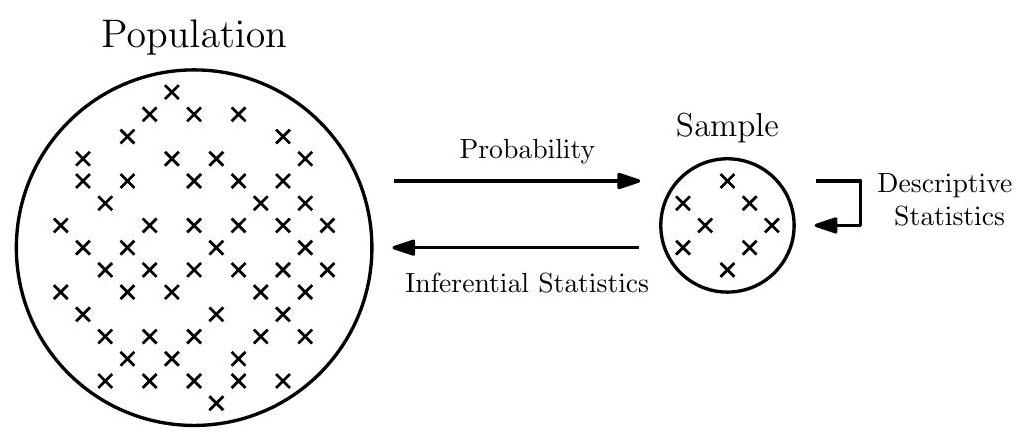
\includegraphics[max width=\textwidth]{2025_03_17_ca60ec0bfd96dcf8e028g-137}
  \caption{The central dogma of statistics: analysis of a small random sample enables drawing rigorous inferences about the entire population.}
\end{figure}

चित्र 5.1 सांख्यिकीय तर्क प्रक्रिया को दर्शाता है। संभावित वस्तुओं की एक नींव जनसंख्या होती है जिसे हम संभावित रूप से देख सकते हैं। उनमें से केवल एक अपेक्षाकृत छोटी उपसमूह का वास्तव में नमूना लिया जाता है, आदर्श रूप में यादृच्छिक रूप से, जिसका अर्थ है कि हम नमूना लिए गए वस्तुओं के गुणों का अवलोकन कर सकते हैं। प्रायिकता सिद्धांत यह वर्णित करता है कि हमारे नमूनों में कौन से गुण होने चाहिए, नींव जनसंख्या के गुणों को देखते हुए। लेकिन \textit{सांख्यिकीय अनुमान} दूसरी दिशा में काम करता है, जहाँ हम नमूना का विश्लेषण करके अनुमान लगाने की कोशिश करते हैं कि पूरी जनसंख्या कैसी है।

आदर्श रूप से, हम एक सांख्यिकीविद की तरह सोचना सीखेंगे: इतना कि अतिशयोक्ति और त्रुटि से सावधान रहें और सुरक्षा बनाए रखें, जबकि डेटा के साथ खेलते रहने और उसे जहां ले जाता है वहां ले जाने के लिए हमारा आत्मविश्वास बना रहे।

\section{सांख्यिकीय वितरण}
प्रत्येक चर का अवलोकन करने पर एक विशेष आवृत्ति वितरण परिभाषित होता है, जो यह दर्शाता है कि प्रत्येक विशेष मान कितनी बार उत्पन्न होता है। ऊंचाई, वजन और आईक्यू जैसी चर की अद्वितीय विशेषताएं उनके वितरणों द्वारा प्रस्तुत की जाती हैं। लेकिन इन वितरणों के आकार स्वयं अद्वितीय नहीं होते: विश्व के विविध डेटा की समृद्धि अक्सर कुछ क्लासिकल रूपों में ही प्रकट होती है।

ये शास्त्रीय वितरण दो अच्छे गुण रखते हैं: (1) वे सामान्यतः व्यवहार में उत्पन्न होने वाले आवृत्ति वितरनों के आकार का वर्णन करते हैं, और (2) उन्हें अक्सर बहुत कम मानकों के साथ बंद-आकृति अभिव्यक्तियों का उपयोग करके गणितीय रूप से वर्णित किया जा सकता है। एक बार जब इन्हें विशेष डेटा अवलोकनों से पृथक कर दिया जाता है, तो वे \textit{संभाव्यता वितरण} बन जाते हैं, जो स्वतंत्र अध्ययन के योग्य होते हैं।

शास्त्रीय प्रायिकता वितरणों के साथ परिचित होना महत्वपूर्ण है। ये अक्सर व्यवहार में आते हैं, इसलिए आपको इनके लिए जागरूक रहना चाहिए। ये हमें यह बताने के लिए एक शब्दावली प्रदान करते हैं कि हमारे डेटा कैसा दिखाई देता है। हम आगे की अनुभागों में सबसे महत्वपूर्ण सांख्यिकीय वितरणों (बाइनोमियल, नॉर्मल, प्वासों और पावर लॉ) की समीक्षा करेंगे, उनके उन गुणों पर विशेष ध्यान देंगे जो उनके आवश्यक चरित्र को परिभाषित करते हैं।\index{eigenvalues}\index{eigenvalues!properties of}\index{matrix!eigenvalues}\index{matrix!eigenvectors}

ध्यान दें कि आपके द्वारा देखे गए आँकड़े किसी विशेष सैद्धांतिक वितरण से उत्पन्न नहीं होते, सिर्फ इसलिए क्योंकि उनका आकार समान है। सांख्यिकीय परीक्षाओं का उपयोग इस बात को कठोरता से सिद्ध करने के लिए किया जा सकता है कि क्या आपके प्रयोगात्मक रूप से देखे गए आँकड़े किसी विशेष वितरण से लिए गए नमूने हैं या नहीं।\index{LU decomposition}\index{matrix!determinant}\index{matrix!triangular}\index{word embeddings}

लेकिन मैं आपको इन परीक्षणों में से किसी भी को वास्तव में चलाने की परेशानी से बचाने जा रहा हूँ। मैं उच्च विश्वास के साथ यह कहूंगा कि आपके वास्तविक-दुनिया के डेटा\textit{सटीक रूप से किसी}प्रसिद्ध सैद्धांतिक वितरणों के अनुरूप नहीं है।

ऐसा क्यों है? समझें कि दुनिया एक जटिल जगह है, जो इसे मापने की प्रक्रिया को उलझन भरा बनाता है। आपके अवलोकन संभवतः विभिन्न नमूना आबादी से लिए जाते हैं, जिनमें से प्रत्येक के पास कुछ हद तक अलग आंतरिक वितरण होता है। आमतौर पर किसी भी देखे गए वितरण के किनारों पर कुछ मजेदार होता है: अचानक असाधारण रूप से उच्च या निम्न मानों का एक उद्वेलन। मापों के साथ त्रुटियाँ जुड़ी होती हैं, कभी-कभी विचित्र प्रणालीगत तरीकों में।

लेकिन जैसा कहा गया है, बुनियादी वितरणों को समझना वास्तव में बहुत महत्वपूर्ण है। प्रत्येक क्लासिकल वितरण क्लासिकल एक कारण की वजह से होता है। इन कारणों को समझना आपको प्रेक्षित आँकड़ों के बारे में बहुत कुछ बताता है, इसलिए इन्हें यहाँ पर समीक्षा की जाएगी।

%---- Page End Break Here ---- Page : 122



\begin{figure}[H]
    \centering
    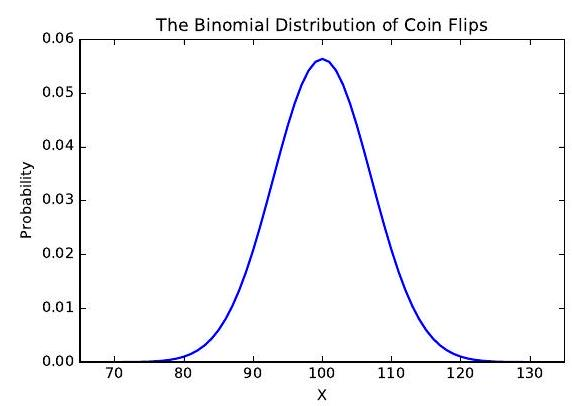
\includegraphics[max width=\textwidth]{2025_03_17_ca60ec0bfd96dcf8e028g-139(1)}
    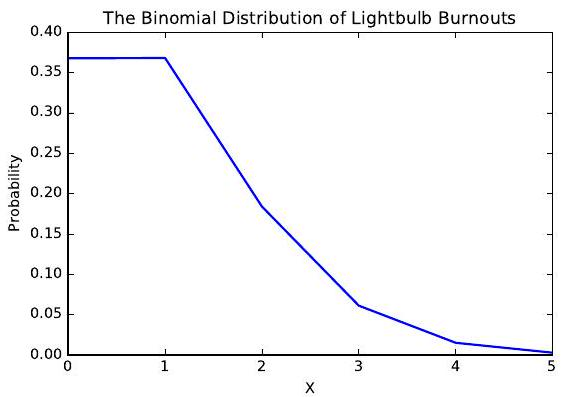
\includegraphics[max width=\textwidth]{2025_03_17_ca60ec0bfd96dcf8e028g-139}
    \caption{The binomial distribution can be used to model the distribution of heads in 200 coin tosses with $p=0.5$ (left), and the number of blown lightbulbs in 1000 events with failure probability $p=0.001$ (right).}
\end{figure}

\subsection{बायनोमीयल वितरण}
एक प्रयोग पर विचार करें जिसमें समान, स्वतंत्र परीक्षण शामिल होते हैं जिनमें दो संभावित परिणाम होते हैं$P_1$और$P_2$, जिनके संभावितता क्रमशः $p$ और $q=(1-p)$ हैं। शायद आपका प्रयोग उच्छेदित सिक्के फेंकना है, जहाँ सिर की संभावना$(p=0.5)$उतनी ही है जितनी पूंछ पाने की$(q=0.5)$। शायद यह बार-बार प्रकाश स्विच चालू करना है, जहाँ अचानक पता चलने की संभावना कि आपको बल्ब बदलना होगा ($p=0.001$) प्रकाश देखने की अपेक्षा काफी कम है ($q=0.999$)।

बायनोमियल वितरण$n$स्वतंत्र प्रयासों के दौरान, विशिष्ट क्रम में नहीं, सही$x P_1$घटनाएँ प्राप्त करने की संभावना को दर्शाता है। स्वतंत्रता यहाँ महत्वपूर्ण है: हम यह मान रहे हैं कि बल्ब के खराब होने की संभावना का इस बात से कोई संबंध नहीं है कि इसे पहले कितनी बार उपयोग किया गया है। बायनोमियल वितरण के लिए पीडीएफ इस प्रकार परिभाषित किया गया है:

\begin{equation}
P(X=x)=\binom{n}{x} p^{x}(1-p)^{(n-x)}
\end{equation}

बायनोमियल वितरण के बारे में कई बातें देखने योग्य हैं:

\begin{itemize}
    \item \textit{यह विविक्त है}: बाइनॉमियल वितरण के लिए दोनों तर्क ($n$ और $x$) पूर्णांक होने चाहिए। चित्र \ref{fig:binomial} (बाएँ) की चिकनाई एक भ्रम है, क्योंकि $n=200$ काफी बड़ा है। 200 सिक्का उछालों में 101.25 हेड्स प्राप्त करने का कोई तरीका नहीं है।
    \item \textit{आप संभवतः इसके पीछे के सिद्धांत को समझा सकते हैं}: आपने सबसे पहले हाई स्कूल में बाइनॉमियल वितरण से सामना किया था। याद है पास्कल का त्रिकोण? विशेष अनुक्रम में ठीक $x$ हेड्स के साथ समाप्त होने की संभावना $n$ फ्लिप्स में होती है $p^{x}(1-p)^{(n-x)}$ प्रत्येक $\binom{n}{x}$ विशेष फ्लिप अनुक्रमों के लिए।
    \item \textit{यह घंटी के आकार का थोड़ा सा होता है}: एक निष्पक्ष सिक्का के लिए $(p=0.5)$, बाइनॉमियल वितरण बिल्कुल सममित होता है, जिसमें औसत मध्य में होता है। यह लाइटबल्ब मामले में सच नहीं है: अगर हम बल्ब को केवल $n=1000$ बार चालू करते हैं, तो विफलताओं की सबसे संभावित संख्या शून्य होगी। यह चित्र \ref{fig:binomial} में सिर्फ आधी घंटी बजाता है। यह कहा गया, जैसे $n \rightarrow \infty$ हम औसत पर चोटी सममित वितरण प्राप्त करेंगे।
    \item \textit{यह केवल दो मापदंडों का उपयोग करके परिभाषित किया जाता है}: एक दिए गए बाइनॉमियल वितरण को पूरी तरह से परिभाषित करने के लिए हमें केवल $p$ और $n$ के मानों की आवश्यकता होती है।
\end{itemize}

कई चीजों को बायनोमियल वितरण द्वारा तर्कसंगत तरीके से मॉडल किया जा सकता है। अनुभाग 2.2.3 में चर्चा किए गए एक$p=0.300$हिटर की प्रदर्शन में परिवर्तनशीलता को याद करें। वहाँ प्रत्येक प्रयास के साथ हिट प्राप्त करने की संभावना$p=0.3$थी, प्रति सीजन$n=500$प्रयासों के साथ। इस प्रकार, प्रति सीजन हिट्स की संख्या को बायनोमियल वितरण से आकर्षित किया जाता है।

यह महसूस करना कि यह द्विपद वितरण था, का अर्थ यह था कि वास्तव में वितरण को बनाने के लिए हमें आवृत्तिपरक करने की आवश्यकता नहीं थी। ऐसे गुणधर्म जैसे कि हिट्स की अपेक्षित संख्या$\mu=n p=500\times0.3=150$और इसका मानक विचलन 
\[
\sigma=\sqrt{n p q}=\sqrt{500 \times 0.3 \times 0.7}= 10.25 
\]
बस संलग्न रूप सूत्रों से निकल जाते हैं जिन्हें आप आवश्यकता पड़ने पर देख सकते हैं।

\subsection{सामान्य वितरण}
\index{normal distribution}कई प्राकृतिक घटनाएँ घंटी के आकार के वक्रों द्वारा मॉडल की जाती हैं। मापी गई विशेषताएँ जैसे ऊँचाई, वजन, आयु सीमा, और आईक्यू सभी एक ही मूल योजना में फिट होते हैं: अधिकांश मान औसत के करीब होते हैं, वितरण सममित होता है, और कोई भी मान बहुत अधिक नहीं होता। दुनिया के सम्पूर्ण इतिहास में, न तो कभी 12 फुट लंबा आदमी हुआ है और न ही 140 साल की औरत।

सभी घंटी-आकार की वक्रों की माँ है\textit{गौसियन}या\textit{सामान्य वितरण}, जो इसकी औसत और मानक विचलन द्वारा पूरी तरह से मापांकित होती है।

\begin{equation}
P(x)=\frac{1}{\sigma \sqrt{2 \pi}} e^{-(x-\mu)^{2} / 2 \sigma^{2}}
\end{equation}

\begin{figure}[H]
    \centering
    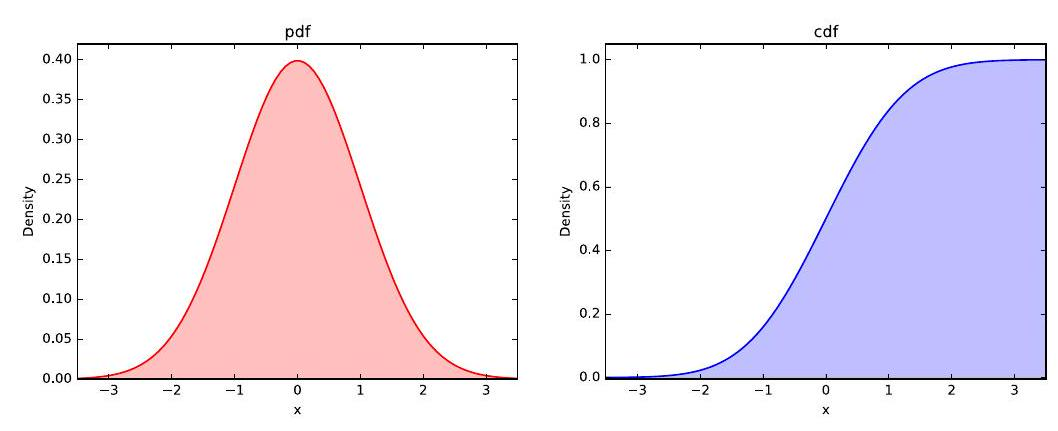
\includegraphics[max width=\textwidth]{2025_03_17_ca60ec0bfd96dcf8e028g-140}
    \caption{The probability density function (pdf) of the normal distribution (left) with its corresponding cumulative density function (cdf) on right.}
\end{figure}

कई बातें ध्यान देने योग्य हैं:

\begin{itemize}
    \item \textit{यह सतत है}: सामान्य वितरण के तर्क (औसत $\mu$ और मानक विचलन $\sigma$) को स्वतंत्र रूप से किसी वास्तविक संख्या में रखा जा सकता है, एकमात्र प्रतिबंध यह है कि $\sigma>0$.
    \item \textit{आप शायद यह नहीं समझा सकते कि यह कहाँ से आता है}: सामान्य वितरण, द्विपद वितरण का सामान्यीकरण है, जहाँ $n \rightarrow \infty$ और औसत के चारों ओर एकत्रीकरण की डिग्री $\sigma$ पैरामीटर द्वारा निर्दिष्ट की जाती है। इस संदर्भ में अपनी अंतर्दृष्टि द्विपद वितरण से लें, और विश्वास करें कि गॉस ने अपनी गणनाएँ सही कीं: महान गणितज्ञ ने अपने पी.एच.डी. शोध प्रबंध के लिए सामान्य वितरण का समाधान किया। या यदि आप वास्तव में जानने के इच्छुक हैं कि यह कहाँ से आता है, तो किसी अच्छी सांख्यिकी पुस्तक से परामर्श लें।
    \item \textit{यह वास्तव में घंटाकृति है}: गाउशन वितरण \index{Gaussian distribution} घंटाकृति वक्र का प्लेटोनिक उदाहरण है। क्योंकि यह एक सतत चर (जैसे ऊँचाई) पर कार्य करता है, न कि एक असतत गणना (जैसे घटनाओं की संख्या) पर, यह पूर्णतः चिकना होता है। क्योंकि यह दोनों दिशाओं में अनंत तक जाता है, किसी भी सिरे पर पूँछ का छँटाई नहीं होती है। सामान्य वितरण एक सैद्धांतिक संरचना है, जो इस पूर्णता को समझाने में मदद करता है।\index{principal components}\index{principal components!analysis}
    \item \textit{यह केवल दो पैरामीटरों का उपयोग करके भी परिभाषित होता है}: हालाँकि, ये द्विपद वितरण से भिन्न पैरामीटर हैं! सामान्य वितरण अपने केंद्रीय बिंदु (औसत द्वारा दिया गया $\mu$) और इसके विस्तार (मानक विचलन द्वारा दिया गया $\sigma$) द्वारा पूर्णतः परिभाषित होता है। ये वे एकमात्र घुंडी हैं जिन्हें हम वितरण को समायोजित करने के लिए उपयोग कर सकते हैं।
\end{itemize}

\section{सामान्य क्या है?}

बहुत से स्वाभाविक रूप से घटित होने वाले घटनाक्रमों को सामान्य वितरण द्वारा मॉडल किया जाता है। शायद सबसे महत्वपूर्ण एक मापन त्रुटि है। हर बार जब आप बाथरूम तराजू पर अपना वजन मापते हैं, तो आपको एक अलग उत्तर मिलेगा, भले ही आपका वजन न बदला हो। कभी-कभी तराजू ऊंचा दिखाएगा और कभी-कभी निम्न, कमरे के तापमान और फर्श के विकटन के अनुसार। छोटे त्रुटियों की संभावना बड़े त्रुटियों से अधिक होती है, और थोड़ा ऊँचा होने की संभावना उतनी ही होती है जितनी कि थोड़ा कम होने की। प्रयोगात्मक त्रुटि सामान्य रूप से \textit{गॉसियन शोर} के रूप में वितरित होती है।

भौतिक घटनाएँ जैसे ऊँचाई, वजन, और जीवनकाल सभी के वितरण बेल के आकार के होते हैं, इसी तरह की दलीलों के साथ। फिर भी, इस तरह के वितरण को \textit{सामान्य} कह देना आमतौर पर बहुत ही आसानी से कर दिया जाता है, बिना गहराई में जाकर यह बताए कि मूल जनसंख्या क्या है। क्या मानव की ऊँचाई सामान्य रूप से वितरित होती है? बिलकुल नहीं: पुरुषों और महिलाओं की औसत ऊँचाई और संबंधित वितरण अलग होते हैं। क्या पुरुषों की ऊँचाई सामान्य रूप से वितरित होती है? बिलकुल नहीं: जब आप बच्चों को शामिल करते हैं और वृद्ध व्यक्तियों के सिकुड़ने को देखते हैं, तो आपके पास फिर से कई अलग-अलग मूल वितरण का योग होता है। क्या संयुक्त राज्य अमेरिका में वयस्क पुरुषों की ऊँचाई सामान्य होती है? नहीं, शायद तब भी नहीं। ऐसे गैर-तुच्छ जनसंख्या समूह हैं जिनमें वृद्धि विकार होते हैं जैसे बौनेपन और एक्रोमेगाली, जो लोगों को या तो सामान्य वितरण द्वारा समझाए जाने की तुलना में काफी छोटा या बड़ा बनाते हैं।

शायद सबसे प्रसिद्ध घंटी के आकार का लेकिन गैर-सामान्य वितरण वित्तीय बाजारों में दैनिक रिटर्न (प्रतिशत मूल्य परिवर्तन) का है। एक बड़ा बाजार दुर्घटना एक बड़े प्रतिशत मूल्य गिरावट द्वारा परिभाषित की जाती है: 10 अक्टूबर, 1987 को Dow Jones औसत ने अपने मूल्य का 22.61% खो दिया। बड़े शेयर बाजार की दुर्घटनाएं सामान्य वितरण द्वारा सटीक रूप से मॉडल की गई से अधिक बार होती हैं। वास्तव में, हर महत्वपूर्ण बाजार दुर्घटना अनियमित रूप से सामान्यता मानने वाले कुछ क्वांट्स को मिटा देती है, और इस तरह की चरम घटनाओं के खिलाफ अपर्याप्त रूप से बीमा करती है। यह निकलता है कि स्टॉक रिटर्न का \textit{लॉगरिदम} सामान्य रूप से वितरित होता है, जिसके परिणामस्वरूप सामान्य से अधिक मोटी पूंछों वाली एक वितरण उत्पन्न होती है।

हालांकि हमें यह याद रखना चाहिए कि घंटी के आकार के वितरण हमेशा सामान्य नहीं होते हैं, बेहतर ज्ञान की अनुपस्थिति में ऐसा मान लेना विचार करना शुरू करने के लिए एक उचित तरीका है।

\subsection{साधारण वितरण के निहितार्थ}

याद रखें कि माध्य और मानक विचलन मिलकर हमेशा किसी भी आवृत्ति वितरण का मोटे तौर पर वर्णन करते हैं, जैसा कि खंड 2.2.4 में चर्चा की गई है। लेकिन वे सामान्य वितरण का विशेष रूप से अच्छा वर्णन करते हैं, क्योंकि वे\textit{सामान्य वितरण को परिभाषित करते हैं}।\index{Jackson, Michael [136]}\index{Spears, Britney [566]}



चित्र\ref{आकृति:सामान्य}सामान्य वितरण का प्रसिद्ध 68\%–95\%–99\% नियम दर्शाता है। अर्थ के क्षेत्र$\pm1\sigma$के भीतर 68 प्रतिशत संभाव्यता संग्रहण होना चाहिए। साथ ही, 95\% संभाव्यता$2\sigma$ के भीतर है, और 99.7\%$3\sigma$ के भीतर।

इसका अर्थ है कि औसत से बहुत दूर मूल्य (के संदर्भ में$\sigma$) किसी भी सामान्य रूप से वितरित चर में अत्यंत दुर्लभ होते हैं। वास्तव में, छह सिग्मा शब्द का उपयोग वर्णन करने के लिए किया जाता है...

%---- Page End Break Here ---- Page : 126

% Mismatched: \sectionname{Poisson Distribution}
The \textit{Poisson distribution} measures the frequency of intervals between rare events. Suppose we model human lifespan by a sequence of daily events, where there is a small but constant probability $1-p$ that one happens to stop breathing today. A lifespan of exactly $n$ days means successfully breathing for each of the first $n-1$ days and then forever breaking the pattern on the $n$th day. The probability of living exactly $n$ days is given by $\operatorname{Pr}(n)=p^{n-1}(1-p)$, yielding an expected lifespan
\[
\mu=\sum_{k=0}^{\infty} k \cdot \operatorname{Pr}(k) .
\]

पोइसन वितरण मूल रूप से इस विश्लेषण से आता है, लेकिन यह$p$ की तुलना में एक अधिक सुविधाजनक दलील लेता है। इसके बजाय, यह$\mu$, वितरण के औसत मूल्य पर आधारित होता है। चूंकि प्रत्येक$p$ एक विशेष$\mu$ मूल्य को परिभाषित करता है, ये पैरामीटर किसी न किसी रूप में समकक्ष होते हैं, लेकिन औसत को अनुमान या मापना बहुत आसान होता है। पोइसन वितरण बहुत सरल बंद रूप देता है:
\[
\operatorname{प्र}(x)=\frac{e^{-\mu} \mu^{x}}{x!}
\]

जब आप सही तरीके से सोचना शुरू करते हैं, तो कई वितरण पोइसोन की तरह दिखने लगते हैं क्योंकि वे दुर्लभ घटनाओं के बीच अंतराल का प्रतिनिधित्व करते हैं।

पिछले खंड से द्विपद वितरण लाइटबुल मॉडल को याद करें। इससे चित्र 5.2 (दाएं) में अपेक्षित परिवर्तनों की संख्या की गणना करना आसान हो गया, लेकिन जीवनकाल वितरण नहीं, जो प्वासां है। चित्र\ref{आकृति:प्वासां-वितरण}से संबंधित प्वासां वितरण को$\mu=1 / p=1000$के लिए प्लॉट करता है, जो दिखाता है कि हम उम्मीद कर सकते हैं कि लगभग सभी बल्ब 900 से 1100 घंटों के बीच जलेंगे, प्रकाश के बुझने से पहले।

\begin{figure}[h]
\centering
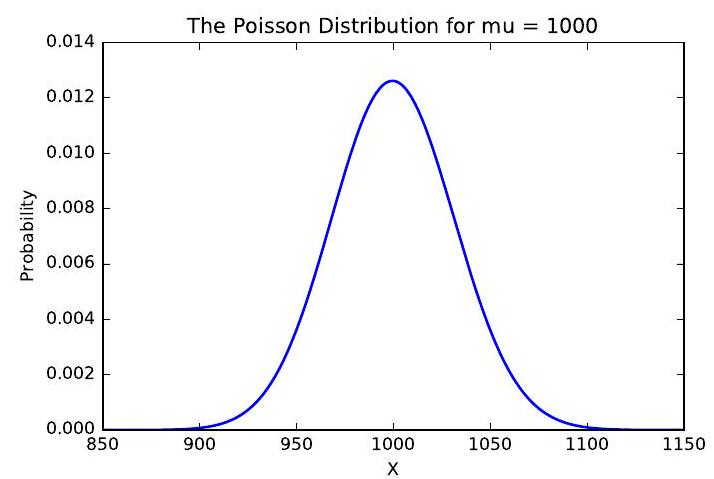
\includegraphics[max width=\textwidth]{2025_03_17_ca60ec0bfd96dcf8e028g-144}
\caption{The lifespan distribution of lightbulbs with an expected life of $\mu=$ 1000 hours, as modeled by a Poisson distribution.}
\label{fig:poisson-distribution}
\end{figure}

वैकल्पिक रूप से, मान लीजिए कि हम बच्चों की संख्या को एक प्रक्रिया के रूप में मॉडल करते हैं जहां परिवार बच्चे पैदा करता रहता है जब तक कि कई अधिक गुस्से, बेक बिक्री या कपड़े धोने के ढेर के बाद, एक माता-पिता अंततः टूट जाते हैं। "बस! मैंने इसका काफी अनुभव कर लिया है। अब और नहीं!"

ऐसे मॉडल के तहत, परिवार के आकार को पॉइसन वितरण के रूप में मॉडल करना चाहिए, जहां हर दिन एक छोटा लेकिन शून्य से अधिक संभावना होती है कि कोई खराबी होगी जिससे फ़ैक्टरी को बंद करना पड़ सकता है।

"मैं अब बर्दाश्त नहीं कर सकता" मॉडल परिवार के आकार की भविष्यवाणी करने में कितना कारगर है? चित्र\ref{fig:family-size}पॉइसन वितरण को दर्शाता है जिसमें पैरामीटर$\lambda=2.2$ है, जिसका अर्थ है कि परिवारों के औसतन 2.2 बच्चे हैं। बिंदु 2010 के अमेरिकी जनरल सोशल सर्वे (GSS) से लिए गए उन परिवारों के अंश को दर्शाते हैं जिनके$k$बच्चे हैं।

\begin{figure}[h]
\centering
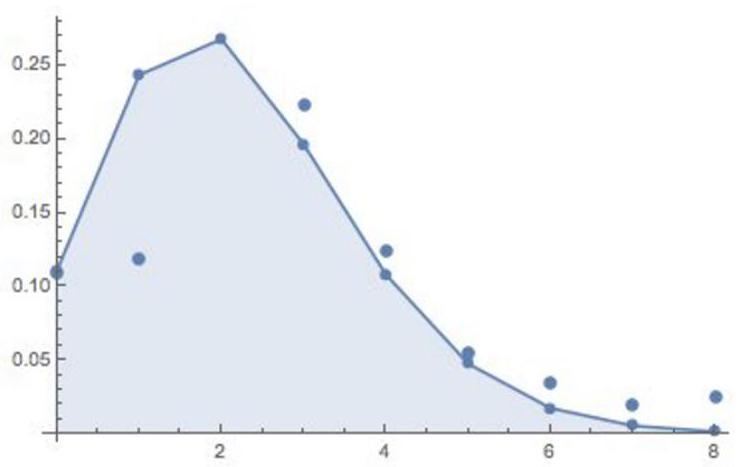
\includegraphics[max width=\textwidth]{2025_03_17_ca60ec0bfd96dcf8e028g-144(1)}
\caption{The observed fraction of families with $x$ kids (isolated points) is accurately modeled by Poisson distribution, defined by an average of $\mu=2.2$ children per family (polyline).}
\label{fig:family-size}
\end{figure}

सभी परिवार के आकारों में उत्कृष्ट अनुकूलता है सिवाय$k=1$, और ईमानदारी से कहूँ, मेरा व्यक्तिगत अनुभव यह सुझाव देता है कि इस डेटा सेट में प्रस्तुत की गई तुलना में अधिक एकल बच्चे हैं। साथ में, केवल औसत और प्वासन वितरण के सूत्र को जानकर हम असली परिवार के आकार के वितरण का एक उचित अनुमान तैयार कर सकते हैं।

% Mismatched: \sectionname{Power Law Distributions}

अनेक डेटा वितरण सामान्य या पोइसन वितरण के तहत संभव से कहीं अधिक लंबी दुम के रूप में प्रदर्शित होते हैं। उदाहरण के लिए, शहरों की जनसंख्या पर विचार करें। विकिपीडिया के अनुसार 2014 में अमेरिका में 100,000 से अधिक लोगों की जनसंख्या वाले ठीक 297 शहर थे। $k$th सबसे बड़े शहर की जनसंख्या, जहाँ $1\leqk\leq297$, चित्र\ref{fig:city-populations} में प्रस्तुत की गई है। यह दिखाता है कि अपेक्षाकृत कम संख्या में शहरों की जनसंख्याएँ बाकी पर अत्यधिक प्रभुत्व जमाती हैं। सच में, सत्रह सबसे बड़े शहरों की जनसंख्या इतनी बड़ी है कि हमने इसे इस आलेख से हटाया है ताकि हम बाकी को देख सकें।

इन शहरों की औसत जनसंख्या 304,689 है, जिसमें 599,816 का भयानक मानक विचलन है। कुछ गलत है जब मानक विचलन औसत के सापेक्ष इतना बड़ा होता है। एक सामान्य वितरण के तहत, $99.7\%$ द्रव्यमान $3\sigma$ औसत के भीतर स्थित है, जिससे यह संभावना नहीं है कि इन शहरों में से किसी की जनसंख्या 2.1 मिलियन से अधिक हो। फिर भी, ह्यूस्टन की जनसंख्या 2.2 मिलियन है, और न्यूयॉर्क (8.4 मिलियन लोगों की जनसंख्या के साथ) औसत से अधिक $13\sigma$ है! शहर की जनसंख्या स्पष्ट रूप से सामान्य रूप से वितरित नहीं है। वास्तव में, वे एक अलग वितरण का पालन करते हैं, जिसे एक पावर लॉ कहा जाता है।

\begin{figure}[h]
\centering
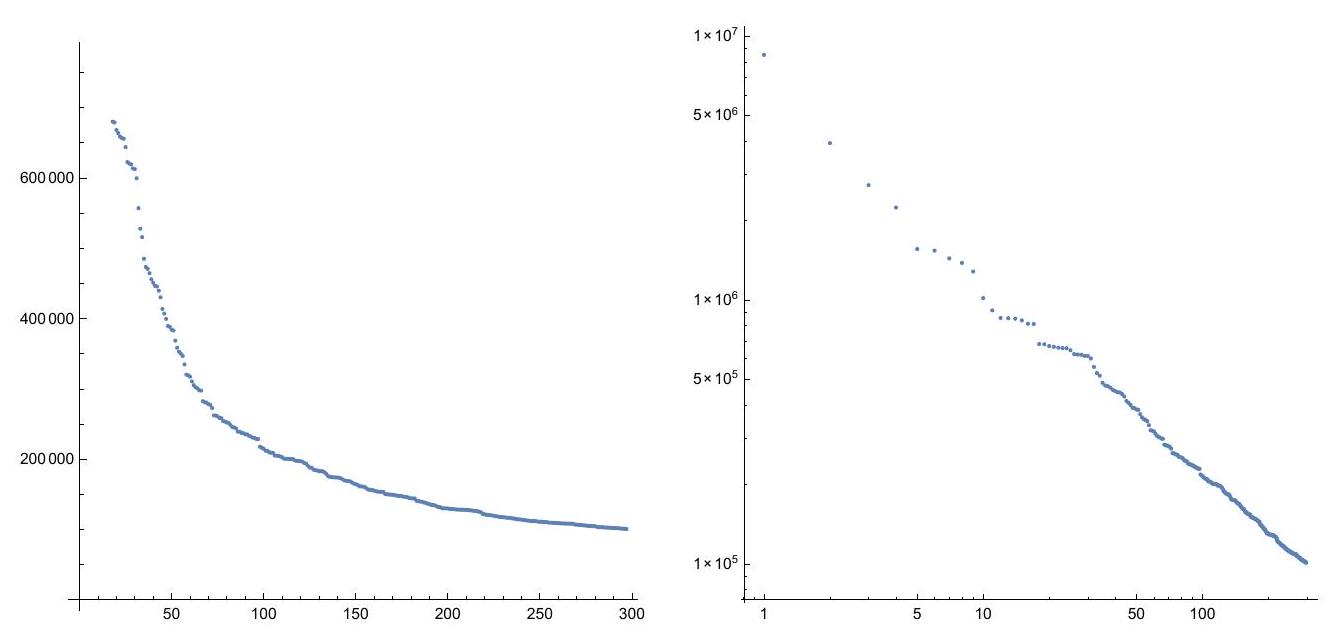
\includegraphics[max width=\textwidth]{2025_03_17_ca60ec0bfd96dcf8e028g-145}
\caption{The population of U.S. cities by decreasing rank (left). On the right is the same data, now including the very largest cities, but plotted on a log-log scale. That they sit on a line is indicative of a power law distribution.}
\label{fig:city-populations}
\end{figure}

दिए गए चर$X$ के लिए जो पॉवर लॉ वितरण द्वारा परिभाषित है, 
\[
P(X=x)=cx^{-\alpha}
\]
इसे दो स्थिरांक से पैरामीटराइज किया गया है: घातांक$\alpha$और सामान्यीकरण स्थिरांक$c$.

पावर लॉ वितरणों को सही तरीके से समझने के लिए कुछ विचार की आवश्यकता होती है। इस वितरण द्वारा परिभाषित कुल प्रायिकता वक्र के नीचे का क्षेत्रफल होती है:
\[
A=\int_{x=-\infty}^{\infty}c x^{-\alpha}=c\int_{x=-\infty}^{\infty}x^{-\alpha}
\]

विशेष मान $A$ उन मानकों से परिभाषित होता है $\alpha$ और $c$। सामान्यीकरण स्थिरांक $c$ को विशेष रूप से दिए गए$\alpha$ के लिए चुना जाता है ताकि सुनिश्चित किया जा सके कि $A=1$, जैसा कि संभावना के नियम मांगते हैं। इसके अलावा,$c$ हमारे लिए किसी विशेष महत्व का नहीं है।\index{coefficient vector}\index{least squares regression}\index{linear regression!solving}\index{matrix}\index{error!residual}\index{linear regression!error}

वास्तविक कार्रवाई $\alpha$ के साथ होती है। ध्यान दें कि जब हम इनपुट का मान दुगुना करते हैं ( $x$ से $2x$ तक), तो हम संभावना को $f=2^{-\alpha}$ के अनुपात से घटा देते हैं। यह बुरा दिखता है, लेकिन किसी भी दिए गए $\alpha$ के लिए यह सिर्फ एक स्थिरांक है। इसलिए जो पावर लॉ वास्तव में कह रहा है वह यह है कि $2x$ आकार की घटना की संभावना $x\alpha आकार की घटना की तुलना में $2^{$}$ गुना कम बार होती है, सभी $x$ के लिए।

व्यक्तिगत सम्पत्ति को एक पावर लॉ द्वारा अच्छी तरह से मॉडल किया जा सकता है, जहाँ$f\approx0.2=1 / 5$. इसका मतलब है कि एक बड़े दायरे में, अगर$Z$लोगों के पास$x$डॉलर्स हैं, तो$Z / 5$लोगों के पास$2x$डॉलर्स हैं। $100,000 के मुकाबले $200,000 के मालिक एक पाँचवां लोग होते हैं। अगर दुनिया में 625 लोग $5 बिलियन की संपत्ति रखते हैं, तो लगभग 125 मल्टी-बिलियिनर होना चाहिए, प्रत्येक की संपत्ति $10 बिलियन है। आगे, $20 बिलियन की संपत्ति वाले 25 सुपरबिलियिनर होने चाहिए, $40 बिलियन स्तर पर पांच हाइपर-बिलियिनर, और अंततः एक बिल गेट्स जिसकी संपत्ति $80 बिलियन है।

पावर लॉज़ "80/20" नियमों को परिभाषित करते हैं जो हमारी दुनिया में सभी विषमताओं के लिए उत्तरदायी हैं: यह अवलोकन कि शीर्ष 20%⸨केA⸩को पूरी तरह से 80%⸨काB⸩मिलता है। पावर लॉज़ तब प्रकट होते हैं जब अमीर और अमीर बनते जाते हैं, जहाँ इस बात की बढ़ती संभावना होती है कि आपको और अधिक मिलेगा, इस आधार पर कि आपके पास पहले से क्या है। बड़े शहर अनुपातहीन रूप से बड़े हो जाते हैं क्योंकि अधिक लोग तब शहरों की ओर आकर्षित होते हैं जब वे बड़े होते हैं। अपनी संपत्ति के कारण, बिल गेट्स को मुझसे कहीं बेहतर निवेश के अवसर मिलते हैं, इसलिए उसका धन मेरे मुकाबले तेजी से बढ़ता है।

कई वितरण को ऐसे प्राथमिकता वाले वृद्धि या संलग्नता मॉडलों द्वारा परिभाषित किया जाता है, जिनमें शामिल हैं:

\begin{itemize}
  \item इंटरनेट साइट्स जिनके $x$ उपयोगकर्ता हैं: वेबसाइटें अधिक लोकप्रिय हो जाती हैं क्योंकि उनके अधिक उपयोगकर्ता होते हैं। आप इंस्टाग्राम या फेसबुक से जुड़ने की संभावना अधिक होती है क्योंकि आपके दोस्त पहले से ही इंस्टाग्राम या फेसबुक से जुड़ चुके हैं। विशेषाधिकार प्राप्त संलग्नता पॉवर लॉ वितरण की ओर ले जाती है।
  \item $x$ सापेक्ष आवृत्ति के साथ उपयोग किए गए शब्द: लाखों शब्दों की एक लंबी सूची है जैसे \textit{ऐल्गोरिस्ट} या \textit{डिफेनेस्ट्रेट}\footnote{डिफेनेस्ट्रेट का अर्थ है "किसी को खिड़की से बाहर फेंकना।"} जो अंग्रेजी भाषा में शायद ही कभी उपयोग किए जाते हैं। दूसरी ओर, \textit{दि} जैसे कुछ शब्द बाकियों की तुलना में कहीं अधिक बार उपयोग किए जाते हैं।
\end{itemize}

ज़िप्फ़ का नियम प्राकृतिक भाषाओं में शब्द उपयोग के वितरण को नियंत्रित करता है और यह कहता है कि सबसे अधिक प्रचलित शब्द (फ्रिक्वेंसी रैंक द्वारा मापा गया) सबसे अधिक प्रचलित शब्द की तुलना में केवल $1/k$ बार ही प्रयोग में आता है। यह देखने के लिए कि यह कितना अच्छा काम करता है, नीचे दी गई अंग्रेज़ी विकिपीडिया में आवृत्तियों के आधार पर शब्दों की रैंकों पर विचार करें:



\begin{tabular}{c|c|c}
Rank & Word & Count \\
\hline
1017 & build & 41890 \\
2017 & essential & 21803 \\
3018 & sounds & 13867 \\
4018 & boards & 9811 \\
5018 & rage & 7385 \\
6019 & occupied & 5813 \\
7020 & continually & 4650 \\
8020 & delay & 3835 \\
9021 & delayed & 3233 \\
10021 & glances & 2767 \\
\end{tabular}

\begin{tabular}{c|c|c}
Rank & Word & Count \\
\hline
10021 & glances & 2767 \\
20026 & ecclesiastical & 881 \\
30028 & zero-sum & 405 \\
40029 & excluded & 218 \\
50030 & sympathizes & 124 \\
60034 & capon & 77 \\
70023 & fibs & 49 \\
80039 & conventionalized & 33 \\
90079 & grandmom & 23 \\
100033 & slum-dwellers & 17 \\
\end{tabular}

\end{center}

यह विश्वास दिलाना चाहिए कि उपयोग की आवृत्ति रैंक के साथ तेजी से घटती है: याद रखें कि \textit{दादीमाँ} केवल \textit{दादी} का एक अनौपचारिक रूप है, वास्तविक नहीं है।

यह एक पावर लॉ क्यों है? एक शब्द जिसकी रैंक$2x$है, उसकी आवृत्ति$F_{2x}\simF_{1}/2x$ होती है, जो$F_{x}\simF_{1}/x$ से तुलना में है। इस प्रकार रैंक को आधा करने पर आवृत्ति दोगुनी हो जाती है, और यह पावर लॉ के$\alpha=1$ से मेल खाती है। 
भाषाओं के विकास के पीछे कौन-सा तंत्र है जो इस वितरण की ओर ले जाता है? एक संभावित व्याख्या यह है कि लोग शब्द सीखते और उपयोग करते हैं क्योंकि वे दूसरों को उनका उपयोग करते हुए सुनते हैं। कोई भी तंत्र जो पहले से लोकप्रिय चीजों को बढ़ावा देता है, वह एक पावर लॉ की ओर ले जाता है।

\begin{itemize}
\item भूकंपों की आवृत्ति $x$ की तीव्रता के परिमाण पर: भूकंप की शक्ति को मापने के लिए रिच्टर पैमाना लघुगणकीय होता है, जिसका अर्थ है कि एक 5.3 का भूकंप 4.3 पैमाने की घटना से दस गुना अधिक शक्तिशाली होता है। परिमाण में एक जोड़ने से शक्ति दस के गुणक से बढ़ जाती है।\\\index{feature scaling}\index{target scaling}\index{non-linear classifiers!fitting}
इतनी तेजी से बढ़ते पैमाने के साथ, यह समझ में आता है कि बड़े घटनाएँ छोटे घटनाओं की तुलना में कम बार होती हैं। मैं हर बार शौचालय फ्लश करने पर 0.02 तीव्रता का भूकंप उत्पन्न करता हूं। वास्तव में, प्रतिदिन ऐसे अरबों घटनाएँ होती हैं, लेकिन बड़े भूकंप बड़े आकार के साथ कम बार होते जाते हैं। जब भी कोई मात्रा प्रकट रूप से अनबाउंडेड तरीके से बढ़ती है लेकिन इसकी संभावना तीव्रता में घटती जाती है, तब आपको एक शक्ति विवर्त (पावर लॉ) मिलता है। आँकड़े दर्शाते हैं कि यह उतना ही सत्य है जितना कि भूकंपों द्वारा मुक्त की गई ऊर्जा और युद्धों के हताहतों की संख्या: दयालुता से, संघर्षों की संख्या जो $x$ व्यक्तियों को मारती है, शक्ति विवर्त के रूप में घटती है।
\end{itemize}

अपने आँखें खुली रखकर पावर लॉ डिस्ट्रीब्यूशन्स को पहचानना सीखें। आपको वे हर जगह हमारी अन्यायपूर्ण दुनिया में मिलेंगे। वे निम्नलिखित गुणों के द्वारा प्रकट होते हैं:

\begin{itemize}
  \item पावर लॉ 'लॉग वैल्यू, लॉग फ्रीक्वेंसी' प्लॉट्स पर सीधी रेखाओं के रूप में प्रकट होते हैं: आकृति \ref{fig:city-populations} में शहर की जनसंख्याओं के ग्राफ की जाँच करें। हालांकि किनारों पर आँकड़े कम होने पर कुछ अंतराल दिखाई देते हैं, लेकिन अधिकांशतः बिंदु एक लाइन पर सटीक रूप से आते हैं। यह पावर लॉ का मुख्य लक्षण है। वैसे, इस रेखा का ढलान $\alpha$ द्वारा निर्धारित होता है, जो पावर लॉ वितरण के आकार को परिभाषित करने वाला स्थिरांक है।
  \item औसत का कोई अर्थ नहीं निकलता: बिल गेट्स अकेले संयुक्त राज्य अमेरिका के औसत व्यक्ति की संपत्ति में लगभग \$250 जोड़ते हैं। यह अजीब है। एक पावर लॉ वितरण के तहत, बहुत छोटी लेकिन गैर-शून्य संभावना होती है कि कोई व्यक्ति अनंत संपत्ति का मालिक होगा, तो यह औसत पर क्या असर करती है? ऐसी वितरणाओं का मुख्य भाग पकड़ने में माध्यम औसत की तुलना में कहीं बेहतर काम करता है।
  \item मानक विचलन का कोई अर्थ नहीं निकलता: एक पावर लॉ वितरण में, मानक विचलन आमतौर पर औसत से बड़ा या बराबर होता है। इसका मतलब है कि वितरण को $\mu$ और $\sigma$ द्वारा बहुत खराब रूप से वर्णित किया जाता है, जबकि पावर लॉ $\alpha$ और $c$ के माध्यम से बहुत अच्छा विवरण प्रस्तुत करता है।
  \item वितरण स्केल इनवेरिएंट है: मान लीजिए कि हमने यू.एस. के 300वें से 600वें सबसे बड़े शहरों की जनसंख्याओं का ग्राफ बनाया, बजाय शीर्ष 300 के, जैसे कि आकृति \ref{fig:city-populations} में। यह आकार बहुत हद तक वही दिखता, 300वें सबसे बड़े शहर की जनसंख्या टेल के ऊपर छाई रहती। कोई भी घातांकी प्रकट स्केल इनवेरिएंट होती है, क्योंकि यह किसी भी रिज़ॉल्यूशन पर एक समान दिखती है। यह इस तथ्य का परिणाम है कि यह 'लॉग-लॉग' प्लॉट पर एक सीधी रेखा होती हैः कोई भी उपभाग एक सीधी लाइन का खंड होता है, जो इसकी खिड़की में पूरे वितरण के समान पैरामीटर के साथ होता है।
\end{itemize}

\subsection{गृह-पाठ का सबक}
शक्ति कानून वितरणों के प्रति सतर्क रहें। वे दुनिया की असमानताओं को दर्शाते हैं, जिसका मतलब है कि वे हर जगह हैं।

\section{वितरण से नमूना लेना}
दिए गए प्रायिकता वितरण से नमूना लेना एक सामान्य प्रक्रिया है, जिसे जानना फायदेमंद होता है। संभवतः आपको कोई सिमुलेशन चलाने के लिए एक शक्ति कानून वितरण से परीक्षण डेटा की आवश्यकता है, या यह सुनिश्चित करने के लिए कि आपका प्रोग्राम चरम परिस्थितियों में काम करता है। यह परीक्षण करना कि आपका डेटा वास्तव में किसी विशेष वितरण के अनुरूप है या नहीं, इसके लिए तुलना करने के लिए कुछ डेटा की आवश्यकता होती है, और वह आम तौर पर पर्याप्त रूप से उत्पन्न सिंथेटिक डेटा होना चाहिए जो मानक वितरण से किया गया हो।\index{power law function}\index{target scaling!sublinear}

किसी भी दिए गए संभावना वितरण से नमूने लेने के लिए एक सामान्य तकनीक होती है, जिसे \textit{इनवर्स ट्रांन्सफॉर्म सैंपलिंग} कहा जाता है। याद करें कि हम संभावना घनत्व फलन$P$ और संचयी घनत्व फलन$C$ के बीच समाकलन और अवकलन द्वारा स्थानांतरित हो सकते हैं। हम उनके बीच आगे-पीछे स्थानांतरित हो सकते हैं क्योंकि:\index{dimension reduction}\index{feature scaling!highly-correlated}\index{New York}\index{target scaling!tipping rate}\index{taxi driver}

\[
P(k=X)=C^{\prime}(k)=C(X \leq k+\delta)-C(X \leq k), \text{ and }
\]

\[
C(X \leq k)=\int_{x=-\infty}^{k} P(X=x)
\]

\begin{figure}[h]
\centering
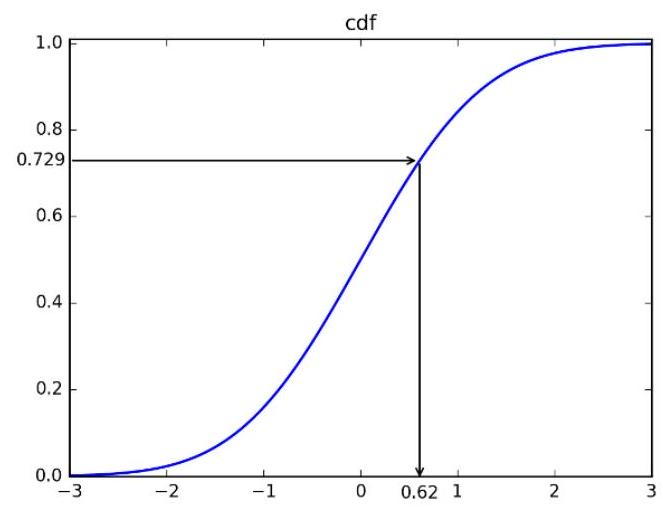
\includegraphics[max width=\textwidth]{2025_03_17_ca60ec0bfd96dcf8e028g-149}
\caption{The inverse transform sampling method enables us to convert a random number generated uniformly from [0,1] (here 0.729) to a random sample drawn from any distribution, given its cdf.}
\label{fig:inverse-transform}
\end{figure}

मान लीजिए कि मैं इस संभवतः बहुत जटिल वितरण से एक बिंदु का नमूना लेना चाहता हूँ। मैं एक समानिक यादृच्छिक संख्या जनरेटर का उपयोग कर सकता हूँ ताकि अंतराल$[0,$, 1]$में एक मान\ldotsp$चुना जा सके। हम$p$को एक प्रायिकता के रूप में व्याख्या कर सकते हैं और इसे संचयी वितरण$C$पर सूचक के रूप में उपयोग कर सकते हैं। सटीक रूप से, हम$x$का वह सही मान रिपोर्ट करते हैं जिसका कि$C(X\leqx)=p$हो।

फ़िगर\ref{fig:inverse-transform}इस दृष्टिकोण को दर्शाता है, यहाँ सामान्य वितरण से सैंपलिंग की जा रही है। मान लीजिए कि$p=0.729$हमारे समरूप जनरेटर से चयनित यादृच्छिक संख्या है। हम$x$मूल्य लौटाते हैं ताकि$y=0.729$, तो इस cdf के अनुसार$x=0.62$।

यदि आप एक लोकप्रिय प्रायिकता वितरण के साथ एक अच्छी तरह से समर्थित भाषा जैसे पाइथन में काम कर रहे हैं, तो लगभग निश्चित रूप से एक पुस्तकालय फ़ंक्शन उपलब्ध होता है जो यादृच्छिक नमूने उत्पन्न कर सकता है। इसलिए, अपनी खुद की लिखने से पहले सही पुस्तकालय की खोज करें।

\subsection{एक आयाम से परे रैंडम सैम्पलिंग}
दी गई वितरण से सही तरीके से सैम्पलिंग करना एक बहुत ही सूक्ष्म समस्या बन जाती है जब आप आयामों की संख्या बढ़ाते हैं। एक वृत के भीतर से बिंदुओं को समान रूप से सैम्पल करने के कार्य पर विचार करें। आगे बढ़ने से पहले एक पल के लिए सोचें कि आप इसे कैसे कर सकते हैं।

%---- Page End Break Here ---- Page : 133

\begin{figure}[H]
    \centering
    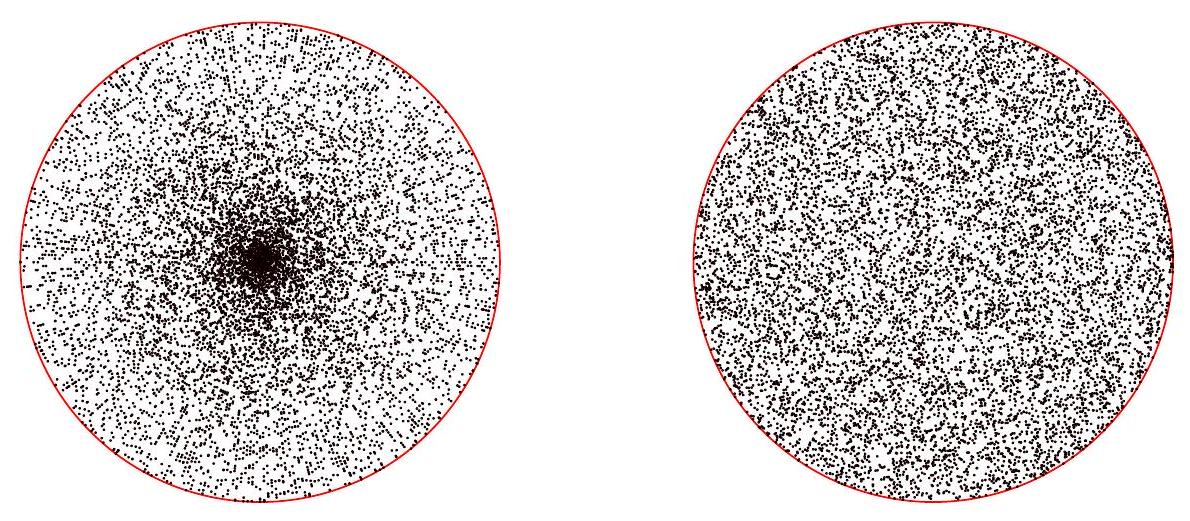
\includegraphics[max width=\textwidth]{2025_03_17_ca60ec0bfd96dcf8e028g-150}
    \caption{Randomly generating 10,000 points by angle-radius pairs clearly oversamples near the origin of the circle (left). In contrast, Monte Carlo sampling generates points uniformly within the circle (right).}
    \label{fig:random_points}
\end{figure}

चतुर व्यक्तियों में से कुछ इस विचार पर पहुँच सकते हैं कि कोण और केन्द्र से दूरी को स्वतंत्र रूप से नमूना लिया जाए। किसी भी नमूना बिंदु को मूल और धनात्मक$x$-अक्ष के साथ जो कोण बनाना चाहिए, वह$0$और$2\piके बीच भिन्न होता है। मूल से दूरी एक मान होना चाहिए जो$0$और$r$के बीच में हो। इन निर्देशांक को समान रूप से यादृच्छिक रूप से चुनें और आपके पास वृत्त में एक यादृच्छिक बिंदु होगा।

यह विधि चतुर है, लेकिन गलत है। निश्चित रूप से, इस प्रकार बनाए गए किसी भी बिंदु को वृत के भीतर ही होना चाहिए। लेकिन बिंदुओं का चयन समान आवृत्ति के साथ नहीं होता। इस विधि से उत्पन्न बिंदुओं में से आधे$r / 2$दूरी के भीतर केन्द्र से स्थित होंगे। लेकिन वृत के अधिकांश क्षेत्र केन्द्र से दूर होता है! इस प्रकार हम मूल के निकट अधिक नमूना लेंगे, जिससे सीमा के निकट द्रव्यमान की क्षति होगी। यह \ref{आकृति:दुर्लभ_बिंदु}(बाएँ) द्वारा दर्शाया गया है, जो इस विधि का उपयोग करके उत्पन्न 10,000 बिंदुओं का प्लॉट है।\index{parameter fitting}

एक साधारण तकनीक जो सही साबित होती है, वह है \textit{मोंटे कार्लो सैंपलिंग}। प्रत्येक बिंदु के$x$और$y$निर्देशांक वृत्त में$-r$से$r$तक होते हैं, जैसे कई बिंदु वृत्त के बाहर भी होते हैं। इस प्रकार, इन मानों को समान रूप से यादृच्छिक रूप से नमूना लेने से हमें एक बिंदु मिलता है जो वृत्त के बाउंडिंग बॉक्स में होता है, लेकिन हमेशा वृत्त के भीतर नहीं। इसे आसानी से परीक्षण किया जा सकता है: क्या $(x, y)$ से मूल तक की दूरी$r$से अधिकतम है, यानी क्या$\sqrt{x^{2}+y^{2}}\leqr$ है? यदि हां, तो हमें वृत्त में एक यादृच्छिक बिंदु मिल गया है। यदि नहीं, तो हम इसे छोड़ देते हैं और फिर से प्रयास करते हैं। चित्र~\ref{fig:random_points}(दायाँ) 10,000 बिंदुओं को इस विधि का उपयोग करके निर्मित करता है: देखें कि कैसे वे समान रूप से वृत्त को कवर करते हैं, जिसमें अधिक या कम सैंपलिंग के कोई स्पष्ट स्थान नहीं हैं।

यहाँ दक्षता पूरी तरह से वांछित क्षेत्र मात्रा (वृत्त का क्षेत्रफल) और सीमाबद्ध बॉक्स मात्रा (वर्ग का क्षेत्रफल) के अनुपात पर निर्भर करती है। चूंकि इस सीमाबद्ध बॉक्स का 78.5% भाग वृत्त द्वारा घेरे हुए है, औसतन दो से कम परीक्षण नए वृत्त के बिंदु को खोजने के लिए पर्याप्त होते हैं।

\begin{figure}[H]
    \centering
    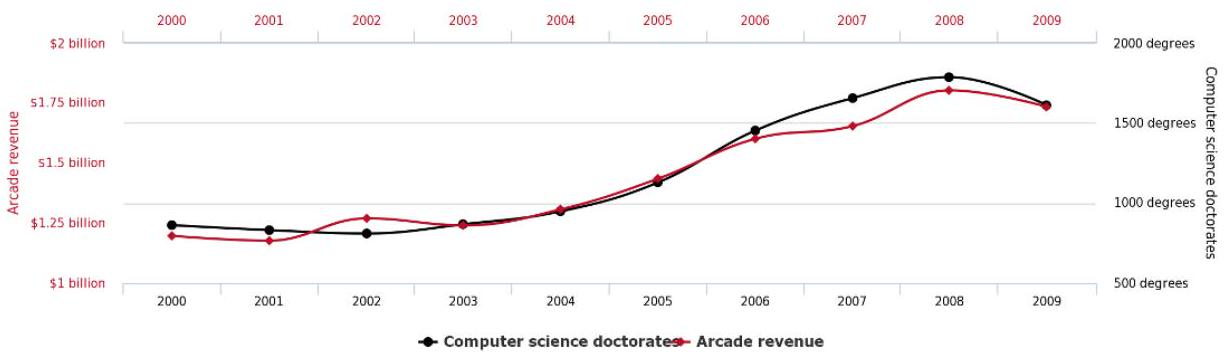
\includegraphics[max width=\textwidth]{2025_03_17_ca60ec0bfd96dcf8e028g-151}
    \caption{Correlation vs. causation: the number of Computer Science Ph.Ds awarded each year in the United States strongly correlates with video/pinball arcade revenue. (from \cite{vigen2015spurious})}
    \label{fig:correlation_vs_causation}
\end{figure}

\section{सांख्यिकीय महत्व}
सांख्यिकीविद मुख्य रूप से इस बात की चिंता करते हैं कि क्या आंकड़ों पर अवलोकन महत्वपूर्ण हैं। गणनात्मक विश्लेषण आसानी से किसी भी दिलचस्प डेटा सेट में एक समूह के रूप में पैटर्न और सहसंबंध पा लेगा। लेकिन क्या एक विशेष सहसंबंध वास्तविक घटना को दर्शाता है, बजाय सिर्फ संयोग के? दूसरे शब्दों में, कब एक अवलोकन \textit{वास्तव में महत्वपूर्ण} होता है?

बड़े डेटा सेट पर पर्याप्त रूप से मजबूत संबंध "स्पष्ट" रूप से सार्थक लग सकते हैं, लेकिन मुद्दे अक्सर काफी सूक्ष्म होते हैं। एक बात यह है कि \textit{संबंध कारणत्व नहीं दर्शाता}। आकृति~\ref{fig:correlation_vs_causation}विश्वसनीय रूप से प्रदर्शित करती है कि कंप्यूटर साइंस में उन्नत अध्ययन की मात्रा का संबंध वीडियो गेम के खेले जाने की मात्रा के साथ है। मैं यह मानना पसंद करता हूँ कि मैंने लोगों को एल्गोरिदम की ओर निनटेंडो से अधिक प्रेरित किया है, लेकिन शायद यह वही बात है? ऐसे गलतफहमी वाले संबंधों के ग्राफ सचमुच एक पुस्तक \cite{vigen2015spurious} में भरे हुए हैं, और वह भी बहुत हास्यजनक।

सांख्यिकी का अनुशासन इस बात पर सूक्ष्म भेद करने में सहायक होता है कि कोई अवलोकन अर्थपूर्ण है या नहीं। चिकित्सा सांख्यिकी से लिया गया एक पारंपरिक उदाहरण दवा उपचारों की प्रभावकारिता निर्धारित करने में आता है। एक औषधि कंपनी दो दवाओं की तुलना का प्रयोग करती है। ड्रग$A$ ने 34 में से 19 मरीजों को ठीक किया। ड्रग$B$ ने 21 में से 14 मरीजों को ठीक किया। क्या ड्रग$B$ सच में ड्रग$A$ से बेहतर है? नई दवाओं को एफडीए द्वारा स्वीकृति मिलने से दवा कंपनियों के मूल्य में अरबों की वृद्धि या कमी हो सकती है। लेकिन क्या आप सुनिश्चित कर सकते हैं कि एक नई दवा वास्तविक सुधार का प्रतिनिधित्व करती है? आप इसे कैसे पता करते हैं?

\subsection{महत्व का महत्व}
सांख्यिकी महत्व यह मापता है कि दो दिए गए वितरणों के बीच एक वास्तविक अंतर होने के प्रति हमारे विश्वास का स्तर कितना है। यह महत्वपूर्ण है। लेकिन सांख्यिकी महत्व इस अंतर के महत्व या परिमाण को नहीं मापता। बड़े\\index{derivative}\index{derivative!second}\index{gradient descent search}\index{derivative!partial}\index{tangent line}

%---- Page End Break Here ---- Page : 135

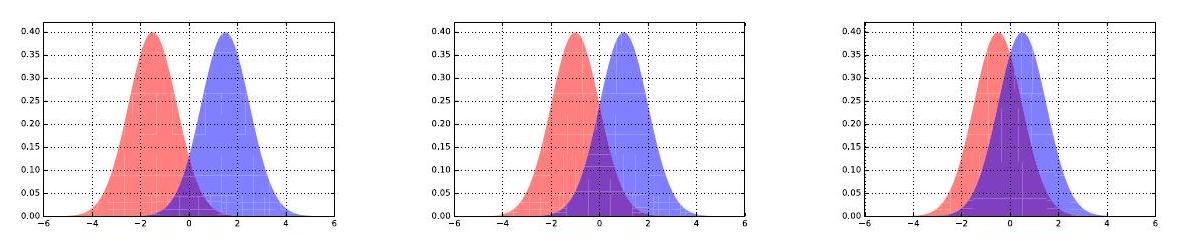
\includegraphics[max width=\textwidth, center]{2025_03_17_ca60ec0bfd96dcf8e028g-152}

\begin{figure}[H]
\centering
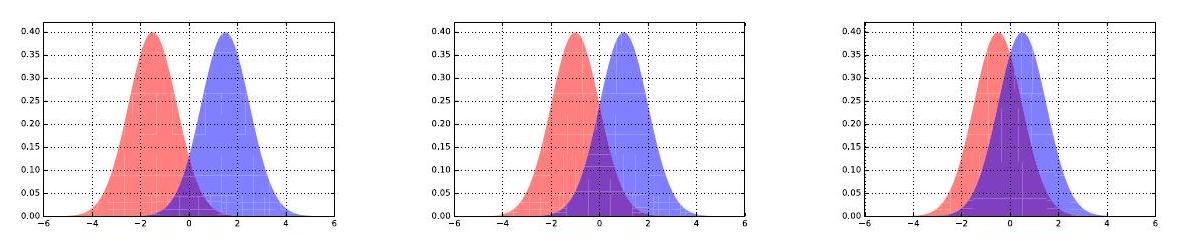
\includegraphics[max width=\textwidth]{2025_03_17_ca60ec0bfd96dcf8e028g-152}
\caption{Pairs of normal distributions with the same variance, but decreasing difference in their means from left to right. As the means get closer, the greater overlap between the distributions makes it harder to tell them apart.}
\end{figure}

पर्याप्त नमूना आकारों के साथ, अत्यंत छोटे अंतर सांख्यिकीय परीक्षणों पर अत्यधिक महत्वपूर्ण के रूप में दर्ज हो सकते हैं।

उदाहरण के लिए, मान लीजिए कि मैं सिक्के पर टेल्स पर बाजी लगाने के चक्कर में पड़ जाता हूँ, जो कि 51\% समय पर हेड्स दिखाता है, इसके बजाय 50\% समय पर जो हम निष्पक्ष सिक्के से जोड़ते हैं। एक निष्पक्ष सिक्के के 100 बार सिक्का उछालने के बाद, मैं 51\% या अधिक हेड्स 46.02\% समय पर देखे जाने की उम्मीद करूँगा, इसलिए मेरे पास कोई शिकायत का आधार नहीं है जब मैं ऐसा करता हूँ। 1,000 बार उछालने के बाद, कम से कम 510 हेड्स देखने की संभावना 0.274 हो जाती है। 10,000 बार उछालने तक, इतने सारे हेड्स देखने की संभावना केवल 0.0233 है, और मुझे यह संदेह होना शुरू हो जाना चाहिए कि क्या सिक्का निष्पक्ष है। 100,000 बार उछालने के बाद, निष्पक्षता की संभावना$1.29\times10^{-10}$ पर आ जाएगी, जो इतनी कम है कि मुझे औपचारिक शिकायत करनी पड़ेगी, भले ही मैंने अपने प्रतिद्वंदी को सज्जन माना हो।

लेकिन यहाँ बात यह है। हालांकि अब यह स्पष्ट है कि मुझे एक पक्षपाती सिक्का इस्तेमाल करने के लिए धोखा दिया गया था, इस कार्रवाई के परिणाम अत्यधिक गंभीर नहीं हैं। जीवन में लगभग किसी भी महत्वपूर्ण मुद्दे के लिए, मैं सिक्के के कम पक्ष को लेने के लिए तैयार रहूँगा, क्योंकि दांव पर्याप्त ऊँचे नहीं हैं। हर एक फ़्लिप पर\$1 दांव लगाने पर, मेरी अपेक्षित नुक़सान 100,000 बार फेंकने के बाद भी केवल\$1,000 बक्स तक होगा।

महत्व आपको यह बताता है कि कुछ केवल संयोग के कारण कितना असंभावित है, लेकिन यह नहीं कि वह महत्वपूर्ण है या नहीं। हम वास्तव में \textit{प्रभाव आकार} की परवाह करते हैं, जो दो समूहों के बीच अंतर की परिमाण होती है। हम अनौपचारिक रूप से \textit{मध्यम}-स्तरीय प्रभाव आकार को एक सावधान पर्यवेक्षक द्वारा नग्न आंखों से दिखाई देने योग्य के रूप में वर्गीकृत करते हैं। इस पैमाने पर, \textit{बड़े} प्रभाव स्पष्ट होते हैं, और \textit{छोटे} प्रभाव पूरी तरह से तुच्छ नहीं होते हैं \cite{sullivan2012effect}. कई सांख्यिकी होते हैं जो प्रभाव आकार को मापने का प्रयास करते हैं, जिनमें शामिल हैं:\index{metric!global}\index{metric!local}\index{Oh G-d!local}

\begin{itemize}
  \item \textit{कोहन का} $d$: दो माध्यों के बीच अंतर का महत्व $\mu$ और $\mu^{\prime}$ परिवर्तन की पूर्ण परिमाण पर निर्भर करता है, लेकिन वितरणों के प्राकृतिक परिवर्तन पर भी निर्भर करता है, जैसा कि $\sigma$ या $\sigma^{\prime}$ से मापा जाता है। इस प्रभाव का आकार मापा जा सकता है: 
\end{itemize}

\[
d=\frac{\left|\mu-\mu^{\prime}\right|}{\sigma}
\]

एक उचित सीमा छोटे प्रभाव आकार के लिए$>0.2$, माध्यम प्रभाव$>0.5$, और बड़ा प्रभाव आकार$>0.8$ है।

\begin{itemize}
  \item \textit{पियर्सन का सहसंबंध गुणांक} $r$: दो चर के बीच रैखिक संबंध की डिग्री को मापता है, -1 से 1 के पैमाने पर। प्रभाव आकार के लिए सीमा रेखाएँ औसत परिवर्तन के समान होती हैं: छोटे प्रभाव $\pm$0.2@ से शुरू होते हैं,
\end{itemize}

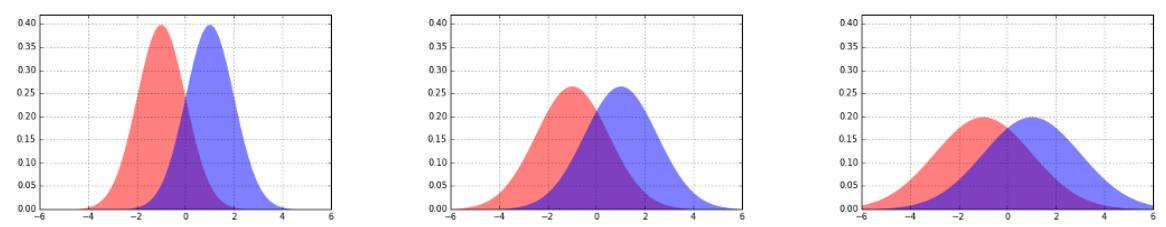
\includegraphics[max width=\textwidth, center]{2025_03_17_ca60ec0bfd96dcf8e028g-153}

\begin{figure}[H]
\centering
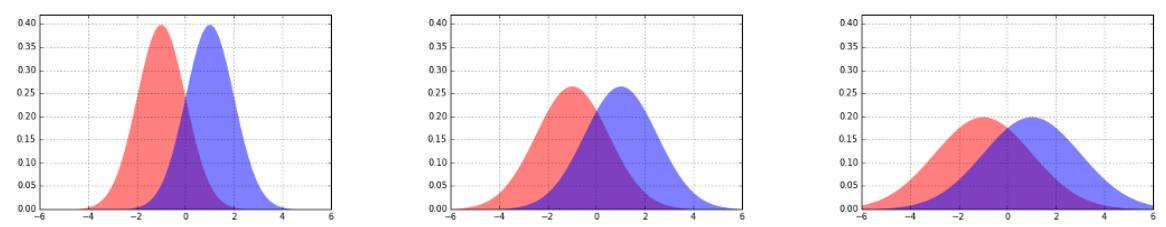
\includegraphics[max width=\textwidth]{2025_03_17_ca60ec0bfd96dcf8e028g-153}
\caption{Pairs of normal distributions with the same difference in their means but increasing variance, from left to right. As the variance increases, there becomes greater overlap between the distributions, making it harder to tell them apart.}
\end{figure}

मध्यम प्रभाव$\pm0.5$ के आसपास होते हैं, और बड़े प्रभाव आकार$\pm0.8$ के सहसंबंधों की आवश्यकता होती है।

\begin{itemize}
  \item \textit{परिवर्तन का गुणांक} $r^{2}$: सहसंबंध गुणांक का वर्ग उस भिन्नता के अनुपात को दर्शाता है जो एक चर में दूसरे द्वारा समझाया जाता है। दिए गए वर्गों की सीमाएँ उन्हें वर्ग करने से प्राप्त होती हैं। छोटे प्रभाव कम से कम 4\% भिन्नता को समझाते हैं, मध्यम प्रभाव $\geq 25\%$ और बड़े प्रभाव आकार कम से कम 64\%।
  \item \textit{अतिव्यापन का प्रतिशत}: किसी भी एकल संभावना वितरण के तहत क्षेत्र, परिभाषा के अनुसार, 1 होता है। दो दिए गए वितरणों के बीच का अंतर्विभाजक क्षेत्र उनकी समानता का एक अच्छा माप है, जैसा कि चित्र 5.11 में दिखाया गया है। समान वितरण 100\% अतिव्यापन करते हैं, जबकि असंबंधित अंतराल 0\% अतिव्यापन करते हैं। तार्किक सीमाएँ हैं: छोटे प्रभावों के लिए 53\% अतिव्यापन, मध्यम प्रभावों के लिए 67\% अतिव्यापन, और बड़े प्रभाव आकार 85\% अतिव्यापन।\index{modeling!simplifying}\index{Occam’s razor}\index{regression!ridge}\index{regularization}\index{target scaling!tipping model}
\end{itemize}

बिल्कुल, किसी भी आकार का प्रभाव जो सांख्यिकीय रूप से महत्वपूर्ण नहीं है, अपने आप में संदेहास्पद होता है। चिट्ठीय विज्ञान (CS) अध्ययन बनाम वीडियो गेम खेलने में सहसंबंध आकृत्ति 5.10 में इतना उच्च था ($r=0.985$) कि प्रभाव आकार विशाल हो सकता था, यदि नमूना बिंदुओं की संख्या और कार्यप्रणाली निष्कर्ष का समर्थन करने के लिए पर्याप्त मजबूत होती।

\textit{घर लेकर जाने का सबक}: सांख्यिकीय महत्वपूर्णता नमूनों की संख्या पर निर्भर करती है, जबकि प्रभाव आकार नहीं करता।

% Mismatched: \sectionname{The T-test: Comparing Population Means}
\index{T-test}We have seen that large mean shifts between two populations suggest large effect sizes. But how many measurements do we need before we can safely believe that the phenomenon is real. Suppose we measure the IQs of twenty men and twenty women. Does the data show that one group is smarter, on average? Certainly, the sample means will differ, at least a bit, but is this difference significant?

टी-टेस्ट का मूल्यांकन करता है कि क्या दो नमूनों के जनसंख्या औसत अलग हैं। यह समस्या सामान्यतः \textit{एबी परीक्षण} में उत्पन्न होती है,\index{AB testing} जो मूल्यांकन करने से जुड़ी होती है।

%---- Page End Break Here ---- Page : 137

% Mismatched: \sectionname{Statistical Analysis}

% Mismatched: \subsectionname{Statistical Significance}

चाहे उत्पाद परिवर्तन प्रदर्शन में अंतर लाता है या नहीं। मान लीजिए आप उपयोगकर्ताओं के एक समूह को संस्करण A दिखाते हैं, और दूसरे समूह को संस्करण B। आगे मान लीजिए कि आप प्रत्येक उपयोगकर्ता के लिए प्रणाली का प्रदर्शन मान मापते हैं, जैसे कि वे कितनी बार विज्ञापनों पर क्लिक करते हैं या जब अनुभव के बारे में पूछा जाता है तो कितने सितारे देते हैं। t-test मापता है कि दो समूहों के बीच देखे गए अंतर का महत्व है या नहीं।

दो मान तब महत्वपूर्ण रूप से भिन्न होते हैं यदि:

\begin{itemize}
\item \textit{माध्यमिक अंतर अपेक्षाकृत बड़ा है:} यह समझ में आता है। कोई आसानी से निष्कर्ष निकाल सकता है कि पुरुषों का औसत वज़न महिलाओं से अधिक होता है, क्योंकि प्रभाव का आकार इतना बड़ा है। सेंटर फ़ॉर डिसीज़ कंट्रोल \footnote{\href{http://www.cdc.gov/nchs/fastats/obesity-overweight.htm}{http://www.cdc.gov/nchs/fastats/obesity-overweight.htm}} के अनुसार 2010 में औसत अमेरिकी पुरुष का वज़न 195.5 पाउंड था, जबकि औसत अमेरिकी महिला का वज़न 166.2 पाउंड था। यह बड़ा अंतर है। एक अधिक सूक्ष्म अंतर जैसे आईक्यू को वास्तविक साबित करने के लिए उतने ही विश्वास के साथ अतिरिक्त साक्ष्य की आवश्यकता होती है। 
\item \textit{मानक विचलन पर्याप्त रूप से छोटे हैं:} यह भी समझ में आता है। खुद को यह विश्वास दिलाना आसान है कि पुरुष और महिलाएँ औसतन समान संख्या में अंगुलियाँ रखते हैं, क्योंकि जो गणना हम देखते हैं वह औसतन बहुत कसकर समुच्चित होती हैं: \(\{10,10,10,10,9,10,\ldots\}\)। समान-अंगुली गिनती परिकल्पना को अधिक सबूत की आवश्यकता होगी यदि संख्याएँ बहुत उछल-कूद करती। मैं \(\mu=10\) के सच्चे वितरणात्मक औसत पर प्रतिबद्ध होने में संकोच करूंगा अगर मैंने \(\{3,15,6,14,17,5\}\) का अवलोकन किया।\index{fit and complexity}
\item \textit{नमूनों की संख्या पर्याप्त बड़ी हैं:} यह फिर से समझ में आता है। जितना अधिक डेटा मैं देखता हूँ, उतना ही दृढ़ता से मुझे विश्वास होता है कि नमूना अपने अंतर्निहित वितरण का सटीक प्रतिनिधित्व करेगा। उदाहरण के लिए, पुरुषों के औसतन महिलाओं से \textit{कम} अंगुलियाँ होती हैं, क्योंकि वे पावर टूल्स के साथ अधिक साहसी होते हैं।\footnote{यह अवलोकन अकेला ही जेंडर-आईक्यू संबंध को हल करने के लिए पर्याप्त हो सकता है, बिना अतिरिक्त सांख्यिकीय साक्ष्य की आवश्यकता के।} लेकिन इस अपेक्षाकृत दुर्लभ घटना का अवलोकन और प्रमाणीकरण करने के लिए एक बहुत बड़ी संख्या में नमूनों की आवश्यकता होगी। 
\end{itemize}

t-परीक्षण दो अवलोकनों के सेटों पर एक परीक्षण सांख्यिकी की गणना से शुरू होता है। वेल्च का t-सांख्यिकी इस प्रकार परिभाषित किया गया है:

\begin{equation}
t=\frac{\bar{x}_{1}-\bar{x}_{2}}{\sqrt{\frac{\sigma_{1}^2}{n_{1}}+\frac{\sigma_{2}^2}{n_{2}}}}
\end{equation}

जहां\(\bar{x}_{i}\),\(\sigma_{i}\), और\(n_{i}\)सैंपल\(i\) के औसत, मानक विचलन, और जनसंख्या आकार को क्रमशः दर्शाते हैं।

चलो हम इस समीकरण को ध्यान से विश्लेषण करें। गुणांक है माध्य के बीच अंतर, तो यह अंतर जितना अधिक होगा, t-सांख्यिकी का मान उतना ही बड़ा होगा। मानक विचलन हर के हिस्से में होते हैं, इसलिए वह\(\sigma_{i}\)जितना छोटा होगा, t-सांख्यिकी का मान उतना ही बड़ा होगा। यदि यह भ्रमित कर रहा है, तो इस बात को ध्यान में रखें कि जब आप\(x\)को शून्य की ओर जाते किसी संख्या से विभाजित करते हैं तो क्या होता है। नमूना आकार\(n_{i}\)को बढ़ाने से भी हर का भाग छोटा होता है, इसलिए\(n_{i}\)जितना बड़ा होगा, t-सांख्यिकी का मान उतना ही बड़ा होगा। सभी मामलों में, वे कारक जो हमें दो वितरणों के बीच वास्तविक अंतर में अधिक विश्वास दिलाते हैं, t-सांख्यिकी के मान को बढ़ाते हैं।

किसी विशेष t-सांख्यिकी के मूल्य की व्याख्या संबंधित तालिका में एक संख्या देखने से होती है। इच्छित\textit{महत्व स्तर}\(\alpha\)और \textit{स्वतंत्रता की डिग्री}(मूल रूप से नमूना आकार), के लिए तालिका प्रविष्टि वह मूल्य\(v\) निर्दिष्ट करती है जिसे t-सांख्यिकी\(t\) को पार करना चाहिए। यदि\(t>v\), तो अवलोकन \(\alpha\)स्तर के लिए महत्वपूर्ण होता है।

\subsection{यह कैसे काम करता है?}

सांख्यिकीय परीक्षण जैसे t-परीक्षण अक्सर मेरे लिए जादू टोना जैसे लगते हैं, क्योंकि हम किसी जादुई तालिका से एक संख्या देखते हैं और इसे किसी पवित्र पुस्तक की तरह मानते हैं।\textit{ज्योतिषी ने कहा है: भिन्नता महत्वपूर्ण है!}बेशक महत्व परीक्षण के पीछे वास्तविक गणित है, लेकिन इसकी व्युत्पत्ति में कैलकुलस और अजीब कार्य (जैसे गामा फंक्शन\(\Gamma(n)\), जो फैक्टरियल्स का वास्तविक संख्या वाला सामान्यीकरण है) शामिल होते हैं। ये जटिल गणनाएँ ही कारण हैं कि पहले से गणना की गई तालिका में चीजों को देखने की परंपरा बनी, बजाय इसके कि आप स्वयं इसे गणना करें।

आप किसी भी अच्छे सांख्यिकी पुस्तक में संबंधित सूत्रों के डेरिवेशन्स देख सकते हैं, यदि आप रुचि रखते हैं। ये परीक्षण ऐसे विचारों पर आधारित हैं जैसे रैंडम सैंपलिंग। हमने देखा है कि माध्य और मानक विचलन किसी भी अंतर्निहित प्रायिकता वितरण के आकार को कैसे नियंत्रित करते हैं। माध्य से बहुत दूर एक नमूना औसत प्राप्त करना खराब भाग्य का संकेत देता है। जनसंख्या के माध्य से कई मानक विचलन की दूरी पर रैंडमली मान चुनना सिद्धांत के अनुसार बहुत असंभव है। इससे यह संभावना बढ़ जाती है कि इतनी बड़ी भिन्नता को देखना एक अलग वितरण से चयनित होने का परिणाम है।

तकनीकीता का बहुत सा हिस्सा यहां सूक्ष्म घटनाओं और छोटे डेटा सेट्स के साथ निपटने के परिणामस्वरूप है। ऐतिहासिक रूप से, देखी गई डेटा एक बहुत ही दुर्लभ संसाधन था, और यह कई परिस्थितियों में अभी भी ऐसा ही है। हमारी दवा की प्रभावकारिता की जांच हेतु चर्चा को याद करें, जहां हर एक बिंदु के लिए किसी नए को मरना पड़ता है जो हम एकत्र करते हैं। बड़ा डेटा वाला संसार जिसमें आप संभवतः रहेंगे, आमतौर पर अधिक आकलन (हर कोई हमारी वेबपेज पर आता है), कम जोखिम (क्या ग्राहक अधिक खरीदते हैं जब आप उन्हें हरे पृष्ठभूमि के बजाय नीले पृष्ठभूमि दिखाते हैं?), और शायद छोटे प्रभाव आकार (हमें वास्तव में कितनी बड़ी सुधार की आवश्यकता है ताकि पृष्ठभूमि का रंग बदलने को उचित ठहराया जा सके?) को दर्शाता है।

\subsection{कोलमोगोरोव-स्मिरनोव परीक्षण}
\index{Kolmogorov-Smirnov test}
t-परीक्षण दो नमूनों की तुलना उनके संबंधित माध्यों के बीच की दूरी के अनुसार करता है, मानते हुए कि वे सामान्य वितरणों से लिए गए हैं। इसके विपरीत, \textit{कोलमोगोरोव-स्मिरनोव} (KS) परीक्षण दो नमूना वितरणों के संचयी वितरण फलनों (cdfs) की तुलना करता है और यह मूल्यांकन करता है कि वे कितने समान हैं।

यह चित्र 5.13 में दर्शाया गया है। दो विभिन्न नमूनों के cdfs को एक ही चार्ट पर प्लॉट किया गया है। यदि दोनों नमूनों को उसी वितरण से लिया गया है, तो उनके \(x\) मूल्यों की सीमाएं बड़े पैमाने पर ओवरलैप होनी चाहिए।

%---- Page End Break Here ---- Page : 139

\begin{figure}[htbp]
	\centering
    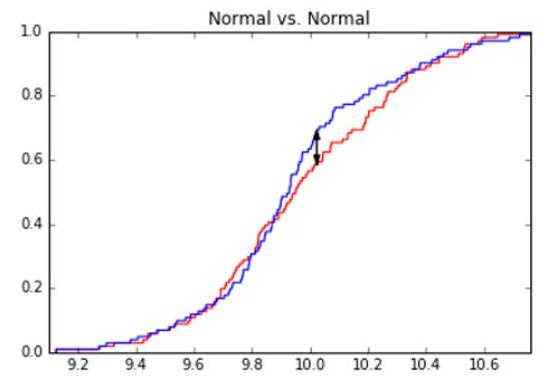
\includegraphics[max width=\textwidth]{2025_03_17_ca60ec0bfd96dcf8e028g-156}
    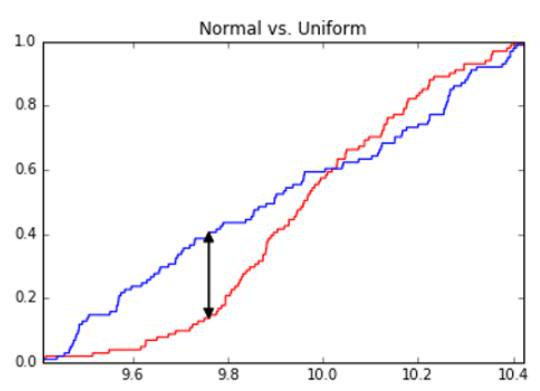
\includegraphics[max width=\textwidth]{2025_03_17_ca60ec0bfd96dcf8e028g-156(1)}
    \caption{The Kolmogorov-Smirnov test quantifies the difference between two probability distributions by the maximum $y$-distance gap between the two cumulative distribution functions. On the left, two samples from the same normal distribution. On the right, comparison of samples from uniform and normal distributions drawn over the same $x$-range.}\index{decision boundaries}\index{logit function}\index{regression!logistic}
    \label{fig:ks-test}
\end{figure}

वितरणों को cdfs के रूप में प्रदर्शित किया जाता है, जहाँ\(y\)-अक्ष 0 से 1 तक संचयी संभावना का प्रतिनिधित्व करता है। दोनों फलन बाएँ से दाएँ एकरूपता से बढ़ते हैं, जहाँ\(C(x)\) नमूने का अनुपात\(\leqx\) है।

हम उस मूल्य की पहचान करना चाहते हैं\(x\)का जिसके लिए जुड़े हुए\(y\)मूल्य दो cdfs के जितना संभव हो सके उतना अंतर रखते हैं। वितरणों के बीच की दूरी\(D\left(C_{1}, C_{2}\right)\)\(C_{1}\)और\(C_{2}\)के बीच\(x\)पर इस महत्वपूर्ण बिंदु पर\(y\)मूल्य का अंतर है, औपचारिक रूप से इसे निम्नलिखित रूप में बताया गया है:

\[
D\left(C_{1}, C_{2}\right)=\max_{-\infty \leq x \leq \infty}\left|C_{1}(x)-C_{2}(x)\right|
\]

जितना अधिक दो नमूना वितरण किसी मूल्य पर भिन्न होते हैं, उतना ही अधिक संभावनाएं होती हैं कि वे अलग-अलग वितरणों से किए गए हैं। चित्र\ref{fig:ks-test}(बाएँ) एक ही सामान्य वितरण से स्वतंत्र नमूने दिखाता है। इनके बीच के बनने वाले छोटे अंतर पर ध्यान दें। इसके विपरीत, चित्र\ref{fig:ks-test}(दाएँ) सामान्य वितरण से खींचे गए एक नमूने की तुलना समान वितरण से खींचे गए नमूने से करता है। केएस-परीक्षण धोखा नहीं खाता: पूंछ के पास बड़े अंतराल को देखें, जहाँ हम इसे देखने की अपेक्षा करते हैं।

के.एस.-टेस्ट दो वितरणों की तुलना एक विशेष लक्ष्य के खिलाफ करता है, यह घोषणा करता है कि दो वितरण महत्वपूर्ण स्तर पर भिन्न हैं जब:

\[
D\left(C_{1}, C_{2}\right)>c(\alpha) \sqrt{\frac{n_{1}+n_{2}}{n_{1} n_{2}}}
\]

जहाँ\(c(\alpha)\)एक स्थिरांक है जिसे एक तालिका में देखा जा सकता है। नमूना आकारों के प्रकट होने के पीछे कुछ अंतर्दृष्टि है। सरलता के लिए मान लें कि दोनों नमूनों का आकार समान है,\(n\)। फिर

\[
\sqrt{\frac{n_{1}+n_{2}}{n_{1} n_{2}}}=\sqrt{\frac{2 n}{n^{2}}}=\sqrt{\frac{2}{n}}
\]

मात्रा\(\sqrt{n}\)स्वाभाविक रूप से सैम्पलिंग समस्याओं में प्रकट होती है, जैसे कि बायनोमियल वितरण का मानक विचलन।\(n\)सिक्के उछालने पर सिरों और पूंछों की संख्या में अपेक्षित अंतर लगभग\(\sqrt{n}\)के क्रम में होता है। केएस-परीक्षण के संदर्भ में, यह समान रूप से दर्शाता है कि जब दो नमूनों को समान माना जाना चाहिए, तब अपेक्षित विचलन क्या होता है। केएस-परीक्षण यह दर्शाता है कि वितरण के आधारभूत हिस्से में क्या हो रहा है, जहां एक मजबूत निर्णय लिया जा सकता है।\index{loss function}

मैं कोल्मोगोरोव-स्मिरनोव टेस्ट पसंद करता हूँ। यह वितरणों की तस्वीरें प्रदान करता है जिन्हें मैं समझ सकता हूँ, जो इस धारणा में सबसे कमजोर बिंदु को पहचानते हैं कि वे एक समान हैं। इस टेस्ट में t-test की तुलना में तकनीकी धारणाएँ और भिन्नताएँ कम हैं, जिसका अर्थ है कि इसका उपयोग करके गलती की संभावना कम है।  और केएस-टेस्ट को कई समस्याओं पर लागू किया जा सकता है, जिसमें यह जांचना भी शामिल है कि ‍बिंदु normaal वितरण से लिए गए हैं या नहीं।

\section{सामान्यता परीक्षण}
\index{normality testing}जब इसे चित्रित किया जाता है, सामान्य वितरण एक घंटीनुमा \index{bell-shaped}वक्र उत्पन्न करता है। लेकिन हर घंटीनुमा वितरण सामान्य नहीं होता है, और कभी-कभी अंतर को जानना महत्वपूर्ण होता है।

दिए गए वितरणीय नमूनों की सामान्यता की जांच के लिए विशेषज्ञ सांख्यिकीय परीक्षण मौजूद हैं\(f_{1}\)। लेकिन हम सामान्य KS-परीक्षण का उपयोग कर सकते हैं, बशर्ते हम\(f_{2}\)को पहचान सकें ताकि\(f_{1}\)से तुलना की जा सके।

यही वजह है कि मैंने खंड 5.2 में रैंडम सैंपलिंग विधियों को पेश किया। जिस संचयी वितरण विधि का हमने वर्णन किया है, उसका उपयोग करके, सांख्यकी-आधारित रैंडम नमूने किसी भी वितरण से लिए जा सकते हैं जिसका आपको cdf पता हो, किसी भी\(n\)के लिए।\(f_{2}\)के लिए, हमें तुलना के लिए एक अर्थपूर्ण बिंदुओं की संख्या चुननी चाहिए। हम\(n_{2}=n_{1}\)का उपयोग कर सकते हैं, या शायद कुछ हद तक बड़ा नमूना यदि\(n_{1}\)बहुत छोटा है। हम यह सुनिश्चित करना चाहते हैं कि हम अपने नमूने के साथ इच्छित वितरण के आकार को सही ढंग से पकड़ रहे हैं।

इसलिए यदि हम सामान्य वितरण से \(f_{2}\) के लिए अपनी यादृच्छिक नमूना बनाते हैं, तो KS-परीक्षण\(f_{1}\) को\(f_{2}\) से अलग नहीं कर पाएगा यदि \(f_{1}\) भी समान \(\mu\)और\(\sigma\) पर सामान्य वितरण से आता है।

एक सावधानी का शब्द। एक पर्याप्त-संवेदनशील सांख्यिकी परीक्षण शायद किसी भी देखी गई वितरिती का सामान्यता को अस्वीकार कर देगा। सामान्य वितरण एक अमूर्त है, और दुनिया एक जटिल जगह है। लेकिन KS-test के प्लॉट को देखकर आपको यह ठीक-ठीक पता चलता है कि विचलन कहाँ हो रहे हैं। क्या पूँछें बहुत मोटी हैं या बहुत पतली? क्या वितरण तिरछा है? इस समझ के साथ, आप यह निर्णय ले सकते हैं कि क्या अंतर आपके लिए पर्याप्त महत्वपूर्ण हैं।

\subsection{बॉन्फेरोनी सुधार}
\index{Bonferroni correction}विज्ञान में लंबे समय से परंपरा रही है कि सांख्यिकीय महत्व और गैर-महत्पूर्ण के बीच\(\alpha=0.05\)को सीमा के रूप में उपयोग किया जाता है। 0.05 की सांख्यिकीय महत्ता का अर्थ है कि इस परिणाम के केवल संयोग से होने की संभावना\(1 / 20\)है।\index{overfitting}

यह एक चुनौतीपूर्ण परिकल्पना की परीक्षा के लिए डाटा एकत्र करने का एक अनुचित मानक नहीं है। 20 से 1 के प्रतिस्पर्धा में घोड़े पर दांव लगाना और अपने दांव को जीतना एक उल्लेखनीय उपलब्धि है। जब तक कि आपने साथ ही लाखों अन्य घोड़ों पर दांव नहीं लगाया हो। तब, उन\(20-1\)दांव के छोटे नंबर के बारे में शेखी बघारना जहां आपने वास्तव में जीता, कम से कम कहने के लिए भ्रामक होगा।

इसलिए मछली पकड़ने के अभियान जो लाखों परिकल्पनाओं का परीक्षण करते हैं, उन्हें उच्च मानकों पर रखा जाना चाहिए। यह वह भ्रांति है जिसने चित्र 5.10 में कंप्यूटर साइंस पीएच.डीज़ और वीडियो गेम गतिविधियों के बीच मजबूत लेकिन असत्य संबंध बना दिया। यह हजारों समय श्रृंखलाओं की एक-दूसरे के खिलाफ तुलना करने के दौरान खोजा गया था, और केवल उन सबसे मनोरंजनपूर्ण जोड़े को बनाए रखा गया जो संयोग से उच्च सहसंबंध स्कोर दिखाते थे।\index{classification!multi-class}\index{scale invariant!ordinal}

बोनफेरोनि करेक्शन\footnote{मैंने हमेशा सोचा है कि "द बोनफेरोनि करेक्शन" एक्शन मूवी के लिए एक शानदार शीर्षक होगा। ड्वेन जॉनसन को बोनफेरोनि के रूप में?}एक महत्वपूर्ण संतुलन प्रदान करता है जब हम किसी प्रत्यक्ष रूप से महत्वपूर्ण सांख्यिकीय परिणाम पर कितना भरोसा करते हैं। यह इस तथ्य की बात करता है कि आप कैसे सहसंबंध को खोजते हैं यह सहसंबंध की ताकत के जितना ही महत्वपूर्ण हो सकता है। कोई व्यक्ति जो एक मिलियन लॉटरी टिकट खरीदता है और एक बार जीतता है, वह उस व्यक्ति की तुलना में कम असरदार करिश्मा रखता है जो एक टिकट खरीदता है और जीतता है।\index{scale invariant!Likert}

बोनफेरोनी सुधार यह बताता है कि जब \(n\) विभिन्न परिकल्पनाओं की एकसाथ जांच की जाती है, तो प्राप्त होने वाला \(p\)-मान को \(\alpha\) स्तर पर महत्वपूर्ण माना जाने के लिए \(\alpha\)/ n@ के स्तर तक बढ़ना चाहिए।

जैसा कि किसी भी सांख्यिकीय परीक्षण के साथ होता है, सही ढंग से सुधार लागू करने में कई सूक्ष्मताएँ होती हैं। लेकिन यहाँ का बड़ा सिद्धांत समझना महत्वपूर्ण है। कंप्यूटिंग लोग विशेष रूप से सभी चीजों के खिलाफ सभी चीजों की बड़े पैमाने पर तुलना चलाने, या असामान्य बाहरी तत्वों और पैटर्न्स की खोज करने की प्रवृत्ति रखते हैं। आखिरकार, एक बार जब आप विश्लेषण प्रोग्राम लिख लेते हैं, तो उसे सभी डेटा पर क्यों न चलाया जाए? केवल सर्वोत्तम, चेरी-पिक किए गए नतीजे प्रस्तुत करने से अन्य लोगों को मूर्ख बनाना आसान हो जाता है। बोनफेरोनी सुधार आपको खुद को मूर्ख बनाने से रोकने का तरीका है।

\subsection{झूठी खोज दर}
बोनफरोनि सुधार हमें कई परीक्षणों में अकेली सफल परिकल्पना की महत्वता को जल्दी से स्वीकार करने से बचाता है। लेकिन अक्सर जब हम बड़े, उच्च-आयामी डेटा के साथ काम कर रहे होते हैं, तो हमें एक अलग समस्या का सामना करना पड़ता है। शायद सभी\(m\)चर उन्मुख यांच्या परिवर्तनीय के साथ सहसंबद्ध होते हैं (शायद कमजोर रूप से)। यदि\(n\)पर्याप्त बड़ा है, तो इन सहसंबंधों में से कई सांख्यिकीय रूप से महत्वपूर्ण होंगे। क्या हमने वास्तव में इतने महत्वपूर्ण खोजें की हैं?\index{Bayes’ theorem}\index{decision tree classifiers}\index{multinomial regression}\index{partition function}

बेन्जामिनी-होचबर्ग प्रक्रिया जो झूठी खोज दर (एफ़डीआर) को न्यूनतम करने की प्रक्रिया है, महत्व के आधार पर रोचक और गैर-रोचक चर के बीच की सीमा खींचने का एक बहुत ही सरल तरीका देती है। चर को उनके\(p\)-मूल्य की शक्ति के अनुसार क्रमबद्ध करें, ताकि अधिक चरम चर बाईं ओर हों, और सबसे कम महत्वपूर्ण चर दाईं ओर हों। अब इस क्रम में\(i\)वें क्रम का चर पर विचार करें। हम इस चर की प्रासंगिकता को इस स्तर पर स्वीकार करते हैं यदि

\[
\forall_{j=1}^{i}\left(p_{j} \leq \frac{j}{m} \alpha\right)
\]

%---- Page End Break Here ---- Page : 142

\section{युद्ध कथा: युवा होने का फव्वारा खोज रहे हैं?}

\begin{figure}[ht]
\centering
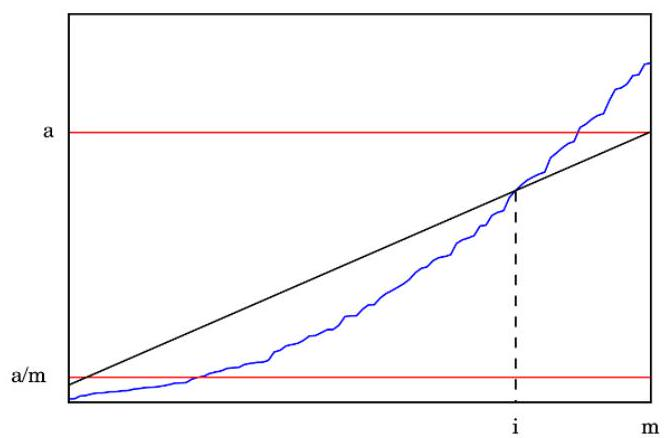
\includegraphics[max width=\textwidth]{2025_03_17_ca60ec0bfd96dcf8e028g-159}
\caption{The Benjamini-Hochberg procedure minimizes false discovery rate, by accepting $p$-values only when $p_{i} \leq \alpha i / m$. The blue curve shows the sorted $p$ values, and the diagonal defines the cutoff for when such a $p$-value is significant.}
\end{figure}

स्थिति को चित्र 5.14 में दर्शाया गया है। ⸨p$⸩-मूल्य को बाएँ से दाएँ बढ़ते क्रम में व्यवस्थित किया गया है, जैसा कि अनियमित नीली वक्र द्वारा दर्शाया गया है। यदि हम सभी ⸨p$⸩-मूल्यों को स्वीकार कर रहे थे जो ⸨$⸩ से कम हैं, तो हम बहुत अधिक स्वीकार कर लेते हैं। यही कारण है कि बोनफेरोनी ने अपना सुधार विकसित किया। लेकिन सभी ⸨p$⸩-मूल्यों को बोनफेरोनी सुधार के मानक को पूरा करने की आवश्यकता (जहाँ वक्र ⸨$/ m\alpha⸩ से टकराती है) अत्यधिक कठोर है।

बेंजामिनी-होचबर्ग प्रक्रिया यह मान्यता रखती है कि यदि कई मान वास्तव में एक निश्चित मानक के लिए महत्त्वपूर्ण हैं, तो उनमें से एक निश्चित अंश को एक बहुत ऊँचे मानक के लिए महत्त्वपूर्ण होना चाहिए। चित्र 5.14 में विकर्ण रेखा इस गुणवत्ता नियंत्रण के स्तर को उपयुक्त रूप से लागू करती है।

यह एक खूबसूरत शादी थी। हमें राचेल और डेविड, दुल्हन और दूल्हे के लिए बहुत खुशी हो रही थी। मैंने राजा की तरह खाया था, अपनी प्यारी पत्नी के साथ नाचा था, और एक सुखद प्राइम रिब के बाद की चमक का आनंद ले रहा था, जब मुझे एहसास हुआ कि कुछ गड़बड़ थी। मैंने कमरे के चारों ओर देखा और दोबारा देखा। किसी तरह, कई वर्षों में पहली बार, मैं भीड़ के अधिकांश लोगों से छोटा हो गया था।

यह आपको बड़ा मुद्दा नहीं लग सकता, लेकिन ऐसा इसलिए है क्योंकि आप, पाठक, शायद\textit{और}कई परिस्थितियों में अधिकांश लोगों से छोटे हैं। लेकिन मुझ पर विश्वास करें, एक समय ऐसा आएगा जब आप ऐसी चीज़ों पर ध्यान देंगे। मुझे याद है जब मैंने पहली बार यह महसूस किया कि मैं कॉलेज में तब पढ़ रहा था जब मेरे अधिकांश छात्र पैदा हो रहे थे। फिर वे तब पैदा होने लगे जब मैं स्नातकोत्तर विद्यालय में था। आज के कॉलेज छात्र केवल तब नहीं पैदा हुए जब मैं प्रोफेसर बना, बल्कि यहां स्थायी नियुक्ति मिलने के बाद जन्मे थे। तो मैं इस शादी में अधिकांश लोगों से छोटा कैसे हो सकता हूं?

वहाँ दो संभावनाएँ थीं। या तो यह संयोगवश था कि इतने अधिक उम्रदराज लोग कमरे में आए, या फिर इस घटना को समझाने के लिए कारण था। यही कारण है कि सांख्यिकीय प्रासंगिकता परीक्षण और$p$-मूल्य आविष्कृत किए गए, ताकि किसी चीज़ को कुछ नहीं से अलग पहचानने में मदद मिल सके।

तो क्या संभावना थी कि मैं, तब 54 वर्ष का, रेचल की शादी में उपस्थित 251 लोगों में से अधिकांश से छोटा होता? वॉलफ्रेम अल्फा के अनुसार \index{Wolfram Alpha}(अधिक सटीक रूप से, 2008-2012 की अमेरिकन कम्युनिटी सर्वे पांच-वर्षीय अनुमान), संयुक्त राज्य अमेरिका में 309.1 मिलियन लोग थे, जिनमें से 77.1 मिलियन की आयु 55 वर्ष या उससे अधिक थी। लगभग सटीक रूप से$25\%$जनसंख्या मुझसे बड़ी है जब मैं ये शब्द लिखता हूँ।

251 यादृच्छिक रूप से चुने गए अमेरिकियों में से अधिकांश के 55 वर्ष से अधिक उम्र के होने की संभावना इस प्रकार दी गई है:

$$
p =\sum_{i=126}^{251}\binom{251}{i}(1-0.75)^{i}(0.75)^{(251-i)}= 8.98\times10^{-18}
$$

यह संभावना असंभव रूप से छोटी है, इसकी तुलना उस स्थिति से की जा सकती है जैसे कि आप अपनी जेब से एक निष्पक्ष सिक्का निकालें और वह लगातार 56 बार हेड्स आए। यह किसी संयोग घटना का परिणाम नहीं हो सकता था। जरूर कोई कारण था कि मैं इस भीड़ में अधिकांश से जूनियर था, और इसका उत्तर यह नहीं था कि मैं किसी भी प्रकार से युवा हो रहा था।

जब मैंने रैचल से इसके बारे में पूछा, तो उसने बताया कि बजट कारणों से उन्होंने बच्चों को शादी में आमंत्रित नहीं करने का फैसला किया। यह एक तार्किक व्याख्या हो सकती है। आखिरकार, इस नियम ने अठारह वर्ष से कम उम्र के 73.9 मिलियन लोगों को शादी में शामिल होने से बाहर रखा, जिससे उन्हें सभी को आमंत्रित करने की बजाय अरबों डॉलर की बचत हुई। मेरे से छोटे लोगों में से जो बच्चे नहीं हैं, उनकी अनुपात$f$इस प्रकार निकलता है$f = 1 - (77.1 / (309.1 - 73.9)) = 0.672$। हालांकि यह 0.5 से काफी बड़ा है। इस समूह से बेतरतीब ढंग से चुने गए नमूने में मेरे औसत से छोटे होने की संभावना इस प्रकार है:

$$
p =\sum_{i=126}^{251}\binom{251}{i}(1-0.0672)^{i}(0.672)^{(251-i)}= 9.118\times10^{-9}
$$

हालाँकि यह पिछले$p$-value से कहीं बड़ा है, फिर भी यह असंभव रूप से छोटा है: मानो आपने अपने निष्पक्ष सिक्के पर लगातार 27 बार हेड्स आने की तरह। केवल बच्चों को मना करना मुझे फिर से जवान बनाने के लिए पर्याप्त शक्तिशाली नहीं था।

मैं वापस जाकर रैचल के पास गया और उसे सच्चाई बताने पर मजबूर किया। पता चला कि उसकी माँ के बचपन में असामान्य रूप से बहुत सारे चचेरे भाई-बहन थे, और वह \textit{सभी}के साथ संपर्क बनाए रखने में असाधारण रूप से अच्छी थी। आइंस्टाइन के सापेक्षता के सिद्धांत को याद करें, \index{theory of relativity} जहाँ$E=mc^{2}$में अर्थ है कि हर कोई मेरी माँ का भाई-बहन है, दो बार हटाया गया। \textit{सभी}इन भाइयों को शादी में आमंत्रित किया गया था। रैचल के परिवार द्वारा दूल्हे के असामान्य रूप से छोटे परिवार को मात देने के साथ, ये वरिष्ठ चचेरे भाई डांस फ्लोर पर हावी होने आए।

वास्तव में, हम उन वृद्ध-चचेरे भाईयों ($c$) की संख्या की गणना कर सकते हैं जिन्हें आमंत्रित करना होगा ताकि मेरे मेहमानों की औसत आयु से कम होने की $50/50$ संभावना हो, यह मानते हुए कि शेष 251 मेहमान यादृच्छिक रूप से चुने गए थे। यह पता चलता है कि

%---- Page End Break Here ---- Page : 144
\clearpage 
\section{Permutation Tests and P-values}

\begin{figure}[htbp]
    \centering
    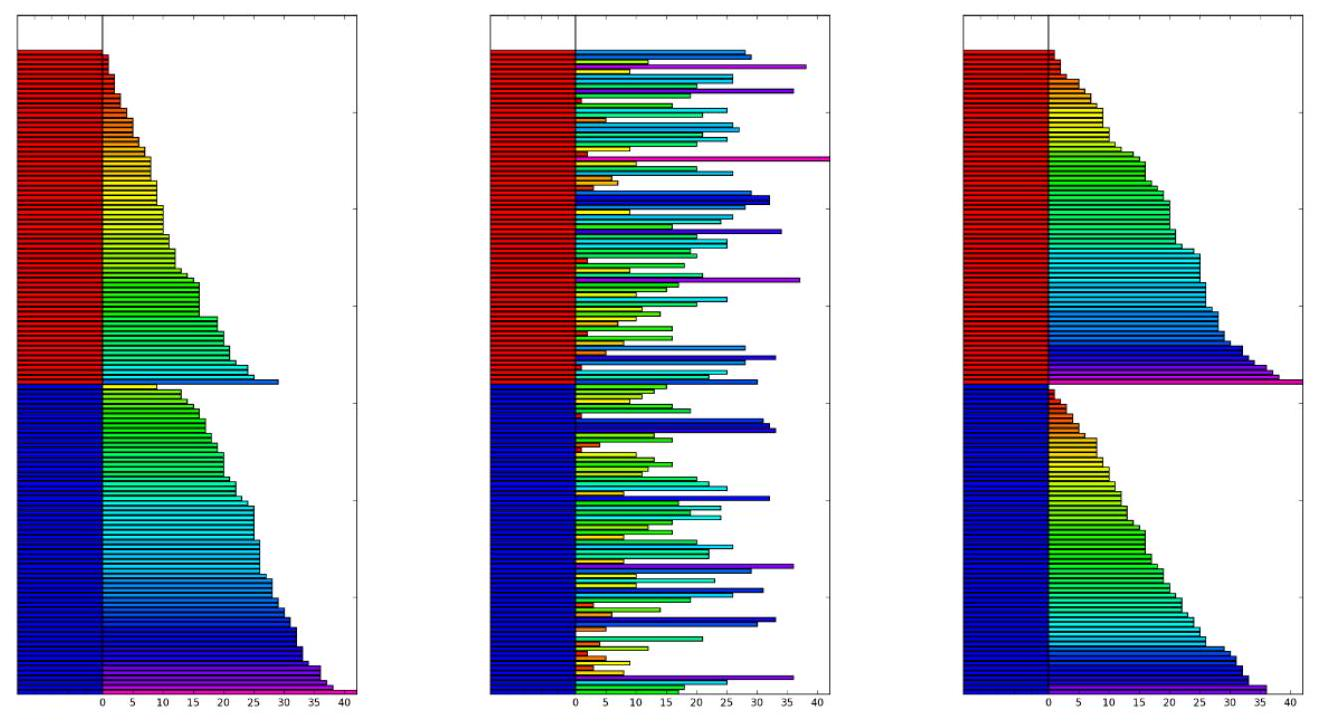
\includegraphics[max width=\textwidth]{2025_03_17_ca60ec0bfd96dcf8e028g-161}
    \caption{Permutation tests reveal the significance of the correlation between gender and the height (left). A random assignment of gender to height (center) results in a substantially different distribution of outcomes when sorted (right), validating the significance of the original relationship.}
\end{figure}

मूल्य$c=65$एकल चचेरे भाई (या 32.5 विवाहित जोड़े) पर्याप्त हैं, जब बच्चों को बाहर रखा गया है ($f=0.672$)।

यहाँ नीतिकथा यह है कि किसी भी रोचक अवलोकन को चमत्कार घोषित करने से पहले उसकी सम्भावना की गणना करना महत्वपूर्ण है। अगर यह आश्चर्य को सम्भावित स्तरों तक कम नहीं करता है, तो आंशिक व्याख्या के साथ कभी न रुकें। किसी भी पर्याप्त दुर्लभ घटना के पीछे शायद कोई वास्तविक घटना छिपी हो, और यह निर्धारित करना कि वह क्या है, डेटा साईंस को रोमांचक बनाता है।\index{distance metrics}\index{metric}\index{metric!identity}\index{metric!positivity}\index{metric!symmetry}\index{metric!triangle inequality}\index{distance metrics!euclidean}\index{distance metrics!manhattan distance}\index{distance metrics!maximum component}

पारंपरिक सांख्यिकीय महत्वपूर्णता परीक्षण यह निर्णय लेने में बहुत प्रभावी साबित होते हैं कि क्या वास्तव में दो नमूने एक ही वितरण से लिए गए हैं। हालांकि, इन परीक्षणों को सही तरीके से किया जाना चाहिए ताकि वे अपना कार्य कर सकें। कई मानक परीक्षणों में सूक्ष्मताएँ होती हैं जैसे कि एक-पक्षीय बनाम द्वि-पक्षीय परीक्षणों के मुद्दे, वितरणात्मक धारणाएँ, और भी बहुत कुछ। इन परीक्षणों को सही तरीके से करना ध्यान और प्रशिक्षण की मांग करता है।

\textit{पर्म्युटेशन परीक्षाएँ} एक अधिक सामान्य और कम्प्यूटेशनली मूर्ख-सबूत तरीका प्रदान करती हैं ताकि महत्व को स्थापित किया जा सके। यदि आपका परिकल्पना डेटा द्वारा समर्थित है, तो यादृच्छिक रूप से उलटे डेटा सैट्स कम संभावना होगी कि वे इसे समर्थन दें। यादृच्छिकीकृत डेटा के विरुद्ध कई परीक्षण संचालित करके, हम सटीक रूप से यह स्थापित कर सकते हैं कि आप जिस घटना का परीक्षण कर रहे हैं, वह कितनी अद्वितीय है।

\begin{figure}[htbp]
    \centering
    \includegraphics[max width=\textwidth]{2025_03_17_ca60ec0bfd96dcf8e028g-162(1)}\\
    \includegraphics[max width=\textwidth]{2025_03_17_ca60ec0bfd96dcf8e028g-162}
    \caption{Permutation tests score significance by the position of the score on actual data against a distribution of scores produced by random permutations. A position on the extreme tail (left) is highly significant, but one within the body of the distribution (left) is uninteresting.}
\end{figure}

चित्र\ref{fig:5.15} पर विचार करें, जहाँ हम स्वतंत्र चर (लिंग: पुरुष या महिला) और आश्रित चर (जैसे, ऊँचाई) को रंगों का उपयोग करके व्यक्त करते हैं। मूल परिणाम रंग वितरण (बाएँ) पुरुषों और महिलाओं के बीच स्पष्ट रूप से अलग दिखता है, जो ऊँचाई में वास्तविक अंतर को दर्शाता है। लेकिन यह अंतर कितना असामान्य है? हम एक नया डेटा सेट बना सकते हैं जिसमें मूल परिणाम चर को यादृच्छिक रूप से लिंग सौंपा जाता है (मध्य में)। प्रत्येक समूह के भीतर क्रमबद्ध करने से स्पष्ट होता है कि परिणामों का छद्म-पुरुष/महिला वितरण अब मूल डेटा की तुलना में कहीं अधिक संतुलित है (दाएँ)। यह दर्शाता है कि लिंग वास्तव में ऊँचाई निर्धारित करने में\textit{आवश्यक}एक महत्वपूर्ण कारक था, इस निष्कर्ष पर हम और अधिक दृढ़ता से विश्वास करेंगे जब यह 1,000 $या$ 1,000,000 @परीक्षणों में बार-बार होगा।

परीक्षण सांख्यिकी का वास्तविक डाटा पर रैंडम क्रमांतरणों से सांख्यिकी मानों के वितरण के बीच क्रमांक महत्व स्तर या \textit{p-मूल्य} को निर्धारित करता है। चित्र \ref{fig:5.16}(बाएँ) दिखाता है कि हम क्या खोज रहे हैं। वास्तविक मान वितरण के बहुत दाएँ स्थित है, महत्वपूर्णता का प्रमाण देता है। दाएँ चित्र में वास्तविक मान वितरण के मध्य में नरम स्थित है, जिससे कोई प्रभाव नहीं होने का संकेत मिलता है।

परमूटेशन परीक्षणों के लिए आवश्यक है कि आप एक सांख्यिकी विकसित करें जो डेटा के बारे में आपके अवधारणा को दर्शाए। अगर आप किसी विशिष्ट जोड़ी के आंतर को स्थापित करना चाहते हैं, तो संबंध गुणांक एक उचित विकल्प है। आदर्श रूप से, वास्तविक डेटा में देखा गया संबंध किसी भी यादृच्छिक परमूटेशन की तुलना में अधिक मजबूत होगा। लिंग-ऊंचाई कड़ी को मान्य करने के लिए, शायद हमारी सांख्यिकी पुरुषों और महिलाओं की औसत ऊंचाई के अंतर को माप सकती है। फिर से, हम उम्मीद करते हैं कि यह वास्तविक डेटा में अधिकांश यादृच्छिक परमूटेशन की तुलना में बड़ा साबित हो।

अपने सांख्यिकीय चुनाव में रचनात्मक बनें: गुणक्रम परीक्षणों की शक्ति यह है कि ये लगभग किसी भी चीज़ के साथ काम कर सकते हैं जो आप अपने मामले को साबित करने के लिए सोच सकते हैं। यह सबसे अच्छा है अगर आपका सांख्यिकीय समता के अवसर को न्यूनतम करता है, क्योंकि आपको अपने परिकल्पना के विरोध में सभी समताओं की गणना करनी होती है।

\textit{घर ले जाने वाला सबक:}पर्म्यूटेशन टेस्ट आपको आपके डेटा की संभावना आपके परिकल्पना के आधार पर देते हैं, जिसका अर्थ है कि सांख्यिकीय मापदंड रैंडम सैंपल वितरण की तुलना में एक अपवाद होगा। यह बिल्कुल उसी तरह नहीं है जैसे कि आपके डेटा के आधार पर आपकी परिकल्पना को साबित करना, जो कि सांख्यिकीय महत्व परीक्षण का पारंपरिक लक्ष्य होता है। लेकिन यह कुछ भी न होने से कहीं बेहतर है।

परमिटेशन परीक्षण का महत्व स्कोर या \textit{p-value} इस बात पर निर्भर करता है कि कितने यादृच्छिक प्रयास किए जाते हैं। हमेशा कम से कम 1,000 यादृच्छिक परीक्षण करने का प्रयास करें, और यदि संभव हो तो अधिक करें। जितनी अधिक परमिटेशन आप आज़माएँगे, आपकी महत्वता \textit{p-value} उतनी ही प्रभावशाली हो सकती है, कम से कम एक बिंदु तक। यदि दिया गया इनपुट वास्तव में सभी $k$! परमिटेशन में सर्वश्रेष्ठ है, तो सबसे चरम \textit{p-value} जो आप प्राप्त कर सकते हैं, वह $1/k$! है, चाहे आप कितने भी यादृच्छिक परमिटेशन आज़माएँ। ओवरसैंपलिंग आपके हर के नामांक को बढ़ा देगी बिना आपके सही आत्मविश्वास को एक भी बिंदु बढ़ाए।

\textit{घर पर सीखने का पाठ:} P-मूल्य की गणना इस\textit{आपका} आत्मविश्वास बढ़ाने के लिए की जाती है कि कोई अवलोकन वास्तविक और दिलचस्प है। यह केवल तभी काम करता है जब आप सही तरीके से परमीटेशन परीक्षण करते हैं, जिससे ऐसे प्रयोगों का निष्पादन होता है जो आश्चर्य के निष्पक्ष माप प्रदान कर सकते हैं।

\subsection{यादृच्छिक क्रमपरिवर्तन उत्पन्न करना}

यादृच्छिक परिमिश्रण उत्पन्न करना एक और महत्वपूर्ण नमूनाकरण समस्या है जिसे लोग अक्सर गड़बड़ कर देते हैं। नीचे दिए गए दोनों एल्गोरिदम आरंभिक परिमिश्रण\(\{1,2,\ldots, n\}\) को मिश्रित करने के लिए यादृच्छिक अदला-बदली के अनुक्रम का उपयोग करते हैं।

लेकिन यह सुनिश्चित करना कि सभी$n$! परिम्युटेशन समान रूप से रैंडम उत्पन्न होते हैं, एक जटिल काम है। वास्तव में, केवल एक ही एल्गोरिदम इसे सही करता है। क्या यह वही है,

\[\]

\begin{aligned}
& \text{के लिए } i=1 \text{ तक } n \text{ करें } a[i]=i ; \\
& \text{के लिए } i=1 \text{ तक } n-1 \text{ करें } \operatorname{स्वैप}[a[i], a[\operatorname{रैंडम}[i, n]]] ;
\end{aligned}

\]

या यह है:

\[\]

\begin{aligned}
और \text{के लिए} i=1 \text{से} n \text{तक} a[i]=i ; \\\index{dimensional egalitarianism}\index{Z-score}
और \text{के लिए} i=1 \text{से} n-1 \text{तक} \operatorname{स्वैप}[a[i], a[\operatorname{रैंडम}[1, n]]] ;
\end{aligned}

\]

इस पर ध्यान से सोचें: यहाँ पर अंतर बहुत सूक्ष्म है। यह इतना सूक्ष्म है कि आप इसे कोड में भी ध्यान नहीं दे सकते। महत्वपूर्ण अंतर है Random के कॉल में 1 या ⸨i⸩। इनमें से कोई एक एल्गोरिदम सही है और कोई एक एल्गोरिदम गलत है। अगर आपको लगता है कि आप बता सकते हैं, तो यह बताएं, क्यों एक काम करता है और दूसरा नहीं करता है।\index{cosine similarity}\index{norms}\index{points vs. vectors}

अगर आप वास्तव में जानना चाहते हैं, तो पहला एल्गोरिथ्म सही है। यह पहले स्थान के लिए 1 से\(n\)तक एक यादृच्छिक तत्व चुनता है, फिर इसे छोड़ देता है और...
%---- पृष्ठ समाप्ति विराम यहाँ ---- पृष्ठ : 147

\begin{figure}[H]
\centering
\includegraphics[max width=\textwidth]{2025_03_17_ca60ec0bfd96dcf8e028g-164}
\caption{The generation frequency of all \(4! = 24\) permutations using two different algorithms. Algorithm 1 generates them with uniform frequency, while algorithm 2 is substantially biased.}
\label{fig:permutation_frequency}
\end{figure}

बाकी पर पुनरावृत्ति करता है। यह यादृच्छिक रूप से क्रमपरिवर्तन उत्पन्न करता है। दूसरा algorithm कुछ तत्वों को पहले समाप्त होने का बेहतर मौका देता है, जिससे यह दिखता है कि वितरण समान नहीं है।

लेकिन यदि आप इसे सैद्धांतिक रूप से सिद्ध नहीं कर सकते हैं, तो आप परिमाण परीक्षण का विचार उपयोग कर सकते हैं। दोनों एल्गोरिदम को कार्यान्वित करें, और प्रत्येक के 1,000,000 रन प्रदर्शन करें, उदाहरण के लिए, \(n=4\) तत्वों का यादृच्छिक परिमाण बनाएं। गिनें कि प्रत्येक एल्गोरिदम कितनी बार \(4! = 24\) भिन्न-भिन्न परिमाण उत्पन्न करता है। ऐसे प्रयोग के परिणाम चित्र\ref{चित्र:परिमाण_आवृत्ति} में दिखाए गए हैं। एल्गोरिदम 1 आश्चर्यजनक रूप से स्थिर सिद्ध होता है, जिसमें 166.1 वृत्तिकाओं का मानक विचलन है। इसके विपरीत, एल्गोरिदम 2 के अंतर्गत सबसे अधिक और सबसे कम आवृत्ति वाली परिमाणों के बीच आठ गुना अंतर है, जिसमें \(\sigma= 20,923.9\) है।

यहाँ नैतिक यह है कि यादृच्छिक उत्पादन अत्यंत सूक्ष्म हो सकता है। और कि मोंटे कार्लो-प्रकार के प्रयोग जैसे कि परमीटेशन परीक्षण सूक्ष्म तर्क की आवश्यकता को समाप्त कर सकते हैं। सत्यापित करें, फिर विश्वास करें।

\section{डिमैggio की हिटिंग स्ट्रीक}
बेसबॉल के कुछ सबसे अद्भुत रिकॉर्ड्स में से एक जो डिमागियो की 56-खेल हिटिंग स्ट्रीक है। एक बल्लेबाज का काम हिट्स प्राप्त करना होता है, और उन्हें प्रत्येक खेल में शायद चार मौके मिलते हैं। यहां तक कि बहुत अच्छे बल्लेबाज भी अक्सर असफल हो जाते हैं।

लेकिन 1941 में, जो डिमैगियो ने 56 लगातार खेलों में हिट्स प्राप्त करके सफलता प्राप्त की, जो वास्तव में एक अद्भुत उपलब्धि थी। उसके बाद के पचहत्तर वर्षों में कोई खिलाड़ी इस रिकॉर्ड के करीब भी नहीं पहुंच सका, और न ही उससे पहले कोई।

लेकिन उसकी करियर की परिप्रेक्ष्य में इतना लंबा सिलसिला कितना असामान्य था? डिमैग-

\begin{figure}[H]
\centering
\includegraphics[max width=\textwidth]{2025_03_17_ca60ec0bfd96dcf8e028g-165}
\caption{The distribution of longest hitting streaks, over 100,000 simulated careers. DiMaggio's actual 56-game hitting streak stands at the very tail of this distribution, thus demonstrating the difficulty of this feat.}
\label{fig:hitting_streaks_distribution}
\end{figure}

जियो ने 1736 खेल खेले, जिसमें 6821 एट बैट में 2214 हिट्स लगाए। इस प्रकार उसे लगभग चार एट बैट के साथ अपने खेलों में हिट्स प्राप्त करने चाहिए \(1-(1-(2214 / 6821))^{4}=79.2\%\)। उस कौशल स्तर वाले किसी व्यक्ति के करियर में ऐसे लगातार गेम की श्रृंखला की प्रायिकता क्या है?

उन लोगों के लिए जो मेरे बेसबॉल के उपमाओं से थक चुके हैं, आइए इसे एक अन्य संदर्भ में रखते हैं। मान लीजिए आप एक छात्र हैं जिसकी परीक्षा में औसत ग्रेड 90 है। आप निश्चित रूप से एक बहुत अच्छे छात्र हैं, लेकिन पूर्ण नहीं। क्या संभावनाएं हैं कि आप लगातार दस परीक्षाओं में 90 से ऊपर स्कोर कर सकते हैं? बीस लगातार परीक्षाओं का क्या? क्या आप संभवतः 56 परीक्षाओं में लगातार हंड्रेड ला सकते हैं?\footnotemark{}\index{Kullback-Leibler divergence}\index{nearest neighbor classification}\index{nearest neighbor classification!advantages}
अगर ऐसी लंबी स्ट्रीक हो जाती है, तो क्या इसका मतलब यह है कि आपने अपनी पढ़ाई को एक नए स्तर पर ले लिया है, या बस आप भाग्यशाली हो गए?

तो जब डिमैगियो का हिटिंग स्ट्रीक था, क्या यह सिर्फ उनकी निर्विवाद कौशल और निरंतरता का प्रत्याशित परिणम था, या फिर वह बस भाग्यशाली रहे? वह अपने या किसी भी समय के बेहतरीन हिटरों में से एक थे, अपने तेरह वर्ष के करियर के हर मौसम में एक ऑल-स्टार। लेकिन हम यह भी जानते हैं कि डिमैगियो वक्त-वक्त पर भाग्यशाली रहे। आखिरकार, वह फिल्म स्टार मर्लिन मुनरो से शादीशुदा थे।

इस प्रश्न को हल करने के लिए, हमने यादृच्छिक संख्याओं का उपयोग करके यह अनुकरण किया कि उसने 1736 खेलों के एक सिंथेटिक "करियर" में कितनी बार हिट हासिल की। प्रत्येक खेल में, अनुकरण किए गए जो को चार बार हिट करने के अवसर मिले और यह सफलतापूर्वक टका\(p=(2214/6821)=0.325\) पर सफल हो गया। इसके बाद हम इस अनुकरण किए गए करियर के दौरान सबसे लंबी हिटिंग स्ट्रीक की पहचान कर सकते थे। 100,000 DiMaggio करियर का अनुकरण करके, हमें स्ट्रीक की आवृत्ति वितरण मिलता है जो उसकी उपलब्धि की दुर्लभता को संदर्भ में डालता है और प्रक्रिया में एक\(p\)-value प्राप्त करता है।

परिणामों को आकृति\ref{fig:hitting_streaks_distribution} में दिखाया गया है। केवल 100,000 सिम्युलेटेड करियर में से 44 में (\(p=0.00044\)) डिमैगियो कम से कम 56 खेलों की श्रृंखला बनाने में सफल रहे। इस प्रकार, यह लंबाई उनके द्वारा अपेक्षित से काफी अधिक है। किसी भी मेजर लीग हिटर की दूसरी सबसे लंबी श्रृंखला केवल 44 खेलों की है, जिससे यह सभी के मुकाबले भी अलग है। लेकिन उन्होंने एक बार निम्न स्तर की प्रतियोगिता में लगातार 61 खेलों में भी हिट किया, जिससे प्रतीत होता है कि उनके पास असाधारण स्थिरता की क्षमता थी।\index{analogies}

हिटिंग स्ट्रीक्स को उन खेलों के बीच रन के रूप में देखा जा सकता है जहाँ हिट्स नहीं होते, और इसे पॉइसन वितरण का उपयोग करके मॉडल किया जा सकता है। लेकिन मोंटे कार्लो सिमुलेशन बिना विस्तृत गणित के उत्तर प्रदान करते हैं। पर्मुटेशन टेस्ट न्यूनतम ज्ञान और बौद्धिक प्रयास के साथ हमें अंतर्दृष्टि देते हैं।

\section{बेज़ियन रीज़निंग}
सशर्त संभावना\(P(A\midB)\)घटना\(A\)की संभावना को मापती है यह जानने पर कि घटना\(B\)घटित हुई है। हम इस पुस्तक में हम सशर्त संभावना पर निर्भर रहेंगे, क्योंकि यह हमें ताजा सबूतों जैसे कि देखे गए डेटा के जवाब में एक घटना में हमारे विश्वास को अपडेट करने की अनुमति देती है।

\textit{बेयस का प्रमेय}शर्तीय संभावनाओं के साथ काम करने के लिए एक महत्वपूर्ण उपकरण है, क्योंकि इससे हम शर्तीय को उलट कर सकते हैं:

\[
P(A \mid B)=\frac{P(B \mid A) P(A)}{P(B)}\index{k-nearest neighbors}
\]

बेज़ प्रमेय के साथ, हम प्रश्न को \(P(\text{परिणाम}\mid\text{डेटा})\) से \(P(\text{डेटा}\mid\text{परिणाम})\) में परिवर्तित कर सकते हैं, जिसे अक्सर गणना करना बहुत आसान होता है। कुछ अर्थों में, बेज़ प्रमेय केवल बीजगणित का परिणाम है, लेकिन यह प्रायिकता के बारे में सोचने का एक अलग तरीका प्रस्तुत करता है।

\begin{figure}[H]
\centering
\includegraphics[max width=\textwidth]{2025_03_17_ca60ec0bfd96dcf8e028g-166}
\caption{Bayes' Theorem in action.}
\label{fig:bayes_theorem}
\end{figure}

चित्र\ref{आकृति:बेस_Sिद्धांत}बेस के सिद्धांत को क्रियान्वित होते हुए दर्शाता है। घटना क्षेत्र में चार में से एक ब्लॉक चुनना शामिल है। जटिल घटनाएँ\(A\)और\(B\)ब्लॉकों के उप-रेंज का प्रतिनिधित्व करती हैं, जहाँ\(P(A)=3/4\)और\(P(B)=2/4=1/2\)है। चित्र से ब्लॉकों की गिनती करके, हम देख सकते हैं कि\(P(A\midB)=1/2\)और\(P(B\midA)=1/3\)है। ये भी बेस के सिद्धांत से सीधे अनुसरण करते हैं:

\[\]

\begin{aligned}
& P(A \mid B)=\frac{P(B \mid A) P(A)}{P(B)}=\frac{(1/3) \cdot(3/4)}{(1/2)}=1/2 \\\index{classification!binary}
& P(B \mid A)=\frac{P(A \mid B) P(B)}{P(A)}=\frac{(1/2) \cdot(1/2)}{(3/4)}=1/3
\end{aligned}

\]

बेयesian रीज़निंग यह दर्शाता है कि एक \textit{प्रायोर प्रायबिलिटी}\(P(A)\)एक नए ऑब्जर्वेशन\(B\mid के सामने कैसे अपडेट होती है ताकि वह पोस्टेरियर प्रायबिलिटी\)P(A\(B)\) प्रदान करे, यह संभावना\(P(B\midA)\) और मार्जिनल प्रायबिलिटी\(P(B)\) के अनुपात के अनुसार होता है। ⸨प्रायोर प्रायबिलिटी⸩\(P(A)\) हमारे प्रारंभिक संसार के अनुमान को दर्शाती है, जिसे अतिरिक्त साक्ष्य\(B\) के आधार पर संशोधित किया जाता है।

बेएसीअन रीजनिंग दुनिया को देखने का एक महत्वपूर्ण तरीका है। राचल और डेविड की शादी में प्रवेश करते ही, मेरी पूर्व धारण यह थी कि उम्र का वितरण वैश्विक स्तर पर जैसा होता है, वैसा ही यहाँ भी होगा। लेकिन मेरी विश्वसनीयता हर बुजुर्ग चचेरा भाई के मिलने के साथ कमजोर होती गई, और आखिरकार वह पूरी तरह टूट गई।

हम अनुभाग 11.1 में Bayesian तर्क का उपयोग करके श्रेणीकारकों का निर्माण करेंगे। लेकिन जब आप डेटा का विश्लेषण करें, तो इस दृष्टिकोण को ध्यान में रखें। प्रत्येक कार्य के लिए आपको यह पूर्व धारणा होनी चाहिए कि उत्तर क्या होना चाहिए, और फिर सांख्यिकीय प्रमाणों के अनुसार संशोधन करें।\index{nearest neighbor classification!finding}

\section{अध्याय नोट्स}
प्रत्येक डेटा वैज्ञानिक को एक अच्छी प्रारंभिक सांख्यिकी पाठ्यक्रम लेना चाहिए। प्रतिनिधित्वात्मक ग्रंथों में फ़्रीडमैन \cite{freedman2007statistics} और जेम्स एट अल. \cite{JWHT13} शामिल हैं। व्हीलान \cite{Whe13} एक सरल परिचय है, जबकि हफ़ \cite{huff2010how} सांख्यिकी के साथ सबसे अच्छी तरह से झूठ बोलने पर क्लासिक ग्रंथ है। \index{kd-trees}

डोनोहो \cite{donoho2015data} आँकड़ा विज्ञान के इतिहास को एक सांख्यिकीविद् के दृष्टिकोण से प्रस्तुत करते हैं। यह प्रभावी ढंग से स्थापित करता है कि आज के अधिकतर प्रमुख सिद्धांतों का विकास मूल रूप से सांख्यिकीविदों द्वारा किया गया था, हालांकि उन सिद्धांतों को तत्काल रूप से व्यापक स्वीकृति नहीं मिली। आधुनिक सांख्यिकीविद् अब इन मामलों में कंप्यूटर वैज्ञानिकों के साथ अधिक संतोषजनक बातचीत करने लगे हैं क्योंकि रुचियां पारस्परिक रूप से एकत्रित हो गई हैं।

विजेन \cite{Vig15} एक रोचक संग्रह प्रस्तुत करता है जो कि दिलचस्प समय श्रृंखलाओं से खींची गईं काल्पनिक सहसंबंधों का है। चित्र 5.10 इसका प्रतिनिधित्व करता है, और इसे अनुमति के साथ पुनः मुद्रित किया गया है।

यह प्रदर्शित किया गया है कि अमेरिकी परिवारों के आकार को प्वासां वितरण द्वारा उचित रूप से फिट किया जा सकता है। वास्तव में, 104 देशों से प्राप्त घरेलू आकार वितरणों के विश्लेषण से पता चलता है कि "मैंने पर्याप्त कर लिया है" मॉडल पूरे विश्व में काम करता है \cite{jennings1999household}।

\section{व्यायाम}

% Mismatched: \subsectionname{Statistical Distributions}

\item[5-2.]
\textit{[5]}यह स्पष्ट करें कि निम्नलिखित The Quant Shop घटना के लिए कौनसा वितरण सबसे उपयुक्त लगता है: बाइनॉमियल, नॉर्मल, पोअसों, या पावर लॉ?

\begin{itemize}
\item[(a)] मिस यूनिवर्स प्रतियोगिता में प्रतियोगियों की सुंदरता। 
\item[(b)] हॉलीवुड स्टूडियो द्वारा निर्मित फिल्मों की कुल आय। 
\item[(c)] बच्चों का जन्म वजन। 
\item[(d)] नीलामी में कला कार्यों की कीमत। 
\item[(e)] क्रिसमस पर न्यूयॉर्क में बर्फ की मात्रा। 
\item[(f)] किसी दिए गए फुटबॉल सीज़न में \(x\) खेल जीतने वाली टीमों की संख्या। 
\item[(g)] प्रसिद्ध लोगों की आयु अवधि। 
\item[(h)] एक दिए गए वर्ष में सोने की दैनिक कीमत। 
\end{itemize}

\item[5-3.]
\textit{[5]}यह मानते हुए कि संबंधित वितरण सामान्य है, निम्नलिखित घटनाओं की संभावना का अनुमान लगाएं:

\begin{itemize}
\item[(a)] कि अगली सौ मींजनों में 70 या उससे अधिक बार सिर आएगा? 
\item[(b)] कि यादृच्छिक रूप से चुने गए व्यक्ति का वजन 300 lbs से अधिक होगा? 
\end{itemize}

\item[5-4.]
\textit{[3]}इतिहास परीक्षा में औसत 100 में से 85 अंक था, जिसमें मानक विचलन 15 था। क्या इस परीक्षा के स्कोर्स का वितरण सममित था? यदि नहीं, तो आप इस वितरण को किस आकृति में देखने की अपेक्षा करेंगे? अपने तर्क को स्पष्ट करें।

\item[5-5.]
\textit{[5]}फेसबुक डेटा दिखाता है कि 50\%फेसबुक उपयोगकर्ताओं के पास सौ या अधिक मित्र हैं। इसके अलावा, औसत उपयोगकर्ता के मित्रों की संख्या 190 है। ये निष्कर्ष फेसबुक उपयोगकर्ताओं के मित्रों की संख्या के वितरण के आकार के बारे में क्या कहते हैं?
\end{enumerate}

\subsection{महत्व परीक्षण}

\begin{enumerate}
\setcounter{क्रमांक}{5}
\item[5-6.]
\textit{[3]} निम्नलिखित घटनाओं में से कौन सी घटनाएं संभवतः स्वतंत्र हैं और कौन सी नहीं?
\begin{itemize}
\item[(क)] सिक्का उछालना।
\end{itemize}
\end{enumerate}

\footnotetext{अगर आप मेरी कक्षा में भाग ले रहे हैं, तो मैं आपको बताता हूँ।}

%---- Page End Break Here ---- Page : 152



\begin{enumerate}
  \setcounter{सूची}{6}
    \item 2010 अमेरिकी समुदाय सर्वेक्षण का अनुमान है कि 15 वर्ष और उससे अधिक उम्र की $47.1 \%$ महिलाएँ विवाहित हैं।
    \begin{enumerate}
      \item इन उम्र के बीच की तीन महिलाओं को यादृच्छिक रूप से चुनें। तीसरी चुनी गई महिला के विवाहित होने की संभावना क्या है जबकि वह अकेली ही विवाहित हो?
      \item तीनों महिलाओं के विवाहित होने की संभावना क्या है?
      \item औसतन, आप एक विवाहित महिला के चयन से पहले कितनी महिलाओं का नमूना लेने की उम्मीद करेंगे? मानक विचलन क्या है?
      \item यदि विवाहित महिलाओं का अनुपात वास्तव में $30 \%$ था, तो आप एक विवाहित महिला के चयन से पहले कितनी महिलाओं का नमूना लेने की उम्मीद करेंगे? मानक विचलन क्या है?
      \item आपके (c) और (d) के उत्तरों के आधार पर, घटना की संभावना घटाने से सफलता तक इंतजार के समय के माध्य और मानक विचलन पर कैसे प्रभाव पड़ता है?
    \end{enumerate}

\itemसिद्ध करें कि पृष्ठ 147 के परिमियोग रचना एल्गोरिथ्म सही ढंग से परिमियोग उत्पन्न करता है, अर्थात समान रूप से यादृच्छिक।

\itemउपलब्ध डेटा$m$पुरुषों और$w$महिलाओं की ऊंचाई के बारे में।

\begin{enumerate}
      \item मैन का उपयोग करें t-परीक्षण यह स्थापित करने के लिए कि क्या पुरुष महिलाओं की तुलना में औसतन लंबे हैं।
      \item एक परिम्यूटेशन परीक्षण का प्रदर्शन करें जो यही बात स्थापित करता है: क्या पुरुष महिलाओं की तुलना में औसतन लंबे हैं।
    \end{enumerate}

\itemखेलकूद के आयोजन में, अच्छी टीमें अक्सर वापसी करती हैं और जीतती हैं। लेकिन क्या यह इसलिए है क्योंकि उन्हें जीतना आता है, या सिर्फ इसलिए क्योंकि लंबे खेल के बाद बेहतर टीम आमतौर पर विजयी होती है? एक रैंडम सिक्के के मॉडल के साथ प्रयोग करें, जहां बेहतर टीम के पास एकल अवधि में दूसरे को मात देने की संभावना$p>0.5$है।$n$अवधियों के खेल के लिए, कितनी बार बेहतर टीम जीतती है, और कितनी बार यह पीछे से आकर जीतती है, दी गई संभावना$p$के लिए? यह वास्तविक खेलों के आंकड़ों से कैसे तुलना करता है?

\itemफरवरी 2 को संयुक्त राज्य अमेरिका में ग्राउंडहॉग डे होता है, जब यह कहा जाता है कि अगर ग्राउंडहॉग अपनी छाया देखता है तो सर्दी के छह और सप्ताह आते हैं। फरवरी 2 को धूप होना ग्राउंडहॉग की इनपुट के रूप में लेने पर, क्या इस परंपरा में कोई पूर्वानुमानी शक्ति है? मौसम रिकॉर्ड्स के आधार पर एक अध्ययन करें, और इस जानवर के पूर्वानुमानों की सटीकता के साथ-साथ इसके सांख्यिकीय महत्व की रिपोर्ट दें।
\index{binary relations}\index{graphs!weighted}\index{matrix!adjacency}\index{networks!induced}

\section{साक्षात्कार प्रश्न}

\begin{enumerate}
  \setcounter{गिनती}{11}
  \item सशर्त प्रायिकता क्या है?
  \item बेयेस प्रमेय क्या है? और यह व्यावहारिक रूप में क्यों उपयोगी है?
  \item आप एक स्पैम पहचान एल्गोरिथम को कैसे सुधारेंगे जो एक भोला बेयेस वर्गीकर्ता का उपयोग करता है?
  \item एक सिक्का दस बार उछाला जाता है और परिणाम दो पूंछ और आठ सिर हैं। आप कैसे बता सकते हैं कि सिक्का निष्पक्ष है? इस परिणाम के लिए $p$-मूल्य क्या है?
  \item अब मान लीजिए कि दस सिक्के प्रत्येक दस बार उछाले जाते हैं, कुल 100 उछालों के लिए। आप कैसे परीक्षण करेंगे कि सिक्के निष्पक्ष हैं?
  \item एक चींटी को एक अनंत लम्बी टहनी पर रखा गया है। चींटी एक चरण पीछे या एक चरण आगे समान संभावना के साथ चल सकती है, विवृति समय चरणों के दौरान। $2 n$ चरणों के बाद चींटी के अपने प्रारंभ बिंदु पर लौटने की संभावना क्या है?
  \item आप सिएटल के लिए एक विमान पर बैठने वाले हैं। क्या आपको छाता लाना चाहिए? आप वहाँ रहने वाले अपने तीन बेतरतीब दोस्तों को बुलाते हैं और प्रत्येक से स्वतंत्र रूप से पूछते हैं कि क्या बारिश हो रही है। प्रत्येक दोस्त के पास आपको सच बताने की $2/3$ संभावना है और झूठ बोलने की $1/3$ संभावना है। सभी तीन दोस्तों ने आपको बताया कि बारिश हो रही है। सिएटल में वास्तव में बारिश हो रही होने की क्या संभावना है?
\end{enumerate}

% Mismatched: \sectionname{Kaggle Challenges}

\begin{enumerate}
  \setcounter{क्रम}{18}
  \item निर्णय करें कि नीलामी में खरीदी गई कार एक खराब खरीद है या नहीं। \href{https://www.kaggle.com/c/DontGetKicked}{https://www.kaggle.com/c/DontGetKicked}
  \item एक निश्चित सप्ताह में किसी उत्पाद की मांग का पूर्वानुमान लगाएं। \href{https://www.kaggle.com/c/grupo-bimbo-inventory-demand}{https://www.kaggle.com/c/grupo-bimbo-inventory-demand}
  \item अगले घंटे में हमें कितनी बारिश मिलेगी? \href{https://www.kaggle.com/c/how-much-did-it-rain}{https://www.kaggle.com/c/how-much-did-it-rain}
\end{enumerate}

\chapter{डेटा का दृश्यांकन}

\epigraph{अपनी सबसे बेहतरीन स्थिति में, ग्राफ़िक्स तर्कसंगतता के उपकरण होते हैं।}{एडवर्ड टफ्टे}

डेटा विज्ञान का एक महत्वपूर्ण पहलू प्रभावी डेटा दृश्‍य़ीकरण है, कम से कम तीन विशिष्ट कारणों के लिएः\index{graphs!dense}\index{graphs!non-simple}\index{graphs!simple}\index{graphs!sparse}\index{graphs!unweighted}\index{graphs!weighted}\index{multiedge}\index{program flow graph}\index{road network}\index{self-loop}\index{simple graph}\index{unweighted graph}\index{weighted graph}

\begin{itemize}
\item\textit{अन्वेषणात्मक डाटा विश्लेषण}: आपका डाटा वास्तव में कैसा दिखता है? जिस चीज़ से आप निपट रहे हैं, उसे समझना किसी भी गंभीर विश्लेषण का पहला कदम है। प्लॉट्स और श्रव्यांकन (विज़ुअलाइज़ेशन) इसे करने का सबसे अच्छा तरीका है जो मैं जानता हूँ।
\item\textit{त्रुटि पहचान}: क्या आपने अपने विश्लेषण में कुछ मूर्खतापूर्ण किया? बिना देखे डाटा को किसी भी मशीन लर्निंग एल्गोरिदम को सौंपना मुसीबत को बुलाने जैसा है। बाहरी बिंदुओं, अपर्याप्त सफाई और गलत धारणाओं के साथ समस्याएँ तुरंत प्रकट हो जाती हैं जब आपका डाटा सही तरह से दृश्यांतरित (विज़ुअलाइज़) किया जाता है। अक्सर कोई सारांश आँकड़ा (77.8% सटीक!) छिपा लेता है कि आपका मॉडल वास्तव में क्या कर रहा है। जो आप सही कर रहे हैं और जो गलत कर रहे हैं उसे सही तरीके से देखना बेहतर प्रदर्शन करने का पहला चरण है।
\item\textit{संचार}: क्या आप जो सीखा है उसे दूसरों के सामने प्रभावी ढंग से प्रस्तुत कर सकते हैं? अर्थपूर्ण परिणाम तभी कार्यान्वयन योग्य होते हैं जब वे साझा किए जाते हैं। एक डेटा वैज्ञानिक के रूप में आपकी सफलता इस पर निर्भर करती है कि आप अन्य लोगों को यह विश्वास दिला सकें कि आप जिस बात पर चर्चा कर रहे हैं, वह वाजिब है। एक तस्वीर 1,000 शब्दों के बराबर होती है, विशेषकर जब आप किसी संदेहपूर्ण दर्शक के सामने प्रस्तुति दे रहे होते हैं।
\end{itemize}

आप शायद ग्रेड स्कूल से ही ग्राफ और चार्ट बना रहे हैं। सर्वव्यापी सॉफ़्टवेयर व्यावसायिक दिखने वाली छवियाँ बनाना आसान बनाता है। तो डेटा विज़ुअलाइजेशन में क्या कठिन है?

उत्तर देने के लिए, मैं एक दृष्टांत प्रस्तुत करता हूँ। मेरी युवावस्था के दौरान एक भयंकर घटना हुई, जो एक आइस स्केटिंग चैंपियन पर हमले से संबंधित थी। एक गुंडे ने उसे छड़ी से उसके घुटने पर मारने की कोशिश की, ताकि उसे आगामी ओलंपिक खेलों से बाहर कर सके। सौभाग्य से, उसने घुटने को नहीं मारा, और वह स्केटर सिल्वर मेडल जीतने में सफल रही।

इस अध्याय में, हम उन सिद्धांतों को समझेंगे जो मानक कथानक डिज़ाइन को कार्यक्षम बनाते हैं, और दिखाएँगे कि वे किस प्रकार गुमराह कर सकते हैं यदि उनका सही तरीके से उपयोग नहीं किया गया। इस अनुभव से, हम आपके इस भावना को विकसित करने का प्रयास करेंगे कि कब ग्राफ धोखा दे सकते हैं, और आप कैसे बेहतर ग्राफ बना सकते हैं।

\section{अन्वेषणात्मक डेटा विश्लेषण}

विशाल डेटा सेट्स के आगमन से विज्ञान के काम करने के तरीके में परिवर्तन आ रहा है। पारंपरिक वैज्ञानिक विधि \textit{अनुमान पर आधारित} है। शोधकर्ता इस बात का सिद्धांत बनाते हैं कि दुनिया कैसे काम करती है, और फिर डेटा के आधार पर इस \textit{अनुमान को समर्थन या खारिज} करने की कोशिश करते हैं। इसके विपरीत, ⸨डेटा आधारित⸩ विज्ञान एक महत्वपूर्ण डेटा सेट को इकट्ठा करके शुरू होता है, और फिर ऐसे पैटर्न खोजता है जो आदर्श रूप से भविष्य के विश्लेषण के लिए ⸨अनुमान⸩ की भूमिका निभाएंगे।

\textit{विेेसूचनात्मक डेटा विश्लेषण} एक दिए गए डेटा सेट में पैटर्न और रुझानों की खोज है। दृश्यण तकनीकें इस खोज में महत्वपूर्ण भूमिका निभाती हैं। अपने डेटा को ध्यानपूर्वक देखना कई कारणों से महत्वपूर्ण है, जिसमें संग्रह/प्रसंस्करण में गलतियों की पहचान, सांख्यिकीय धारणाओं के उल्लंघन को खोजने और दिलचस्प परिकल्पनाओं का सुझाव देना शामिल है।

इस खंड में, हम चर्चा करेंगे कि अन्वेषणात्मक डेटा विश्लेषण कैसे किया जाए, और प्रक्रिया के भाग के रूप में दृश्यांकन क्या लाभ प्रदान करता है।

\subsection{नए डेटा सेट का सामना करना}

जब आप एक नए डेटा सेट का सामना करते हैं तो आपको क्या करना चाहिए? यह कुछ हद तक इस पर निर्भर करता है कि आप पहली बार में इसमें क्यों रुचि रखते हैं, लेकिन खोज की प्रारंभिक चरण लगभग एप्लीकेशन-स्वतंत्र होते हैं।

यहाँ कुछ बुनियादी कदम दिए गए हैं जो मैं किसी भी नए डेटा सेट से परिचित होने के लिए करने की सलाह देता हूँ, जिसे मैं शरीर के माप डेटा सेट NHANES का अन्वेषण करने में दर्शाता हूँ, उपलब्ध है \href{https://www.statcrunch.com/app/index.php?dataid=1406047}{https://www.statcrunch.com/app/index.php?dataid=1406047}। यह टेबलर डेटा है, लेकिन यहाँ के सामान्य सिद्धांत व्यापक श्रेणी के संसाधनों पर लागू होते हैं:\index{connected components}\index{edge cuts}\index{matchings}\index{minimum spanning tree}\index{shortest paths}\index{topological sorting}

\begin{itemize}
  \item \textit{मूल प्रश्नों का उत्तर दें}: अपनी फ़ाइल खोलने से पहले, अपने डेटा सेट के बारे में कई बातें जानना आवश्यक होता है। ऐसे प्रश्न पूछें जैसे:
\end{itemize}

%---- Page End Break Here ---- Page : 156

\item\textit{इस डाटा सेट का निर्माण किसने किया, कब और क्यों?} यह समझना कि आपका डाटा कैसे प्राप्त हुआ, यह संकेत देता है कि यह कितना प्रासंगिक हो सकता है और क्या हमें इस पर भरोसा करना चाहिए। यह हमें सही लोगों की ओर भी इंगित करता है यदि हमें डाटा की उत्पत्ति या स्रोत के बारे में अधिक जानने की आवश्यकता है। थोड़ी छानबीन करने पर, मैंने पाया कि यह नेशनल हेल्थ एंड न्यूट्रिशन एग्जामिनेशन सर्वे 2009-2010 से आया है, और इसे प्रकाशित करने की जिम्मेदारी किसकी थी।

\item\textit{यह कितना बड़ा है?} डेटा सेट के समृद्धि का मूल्यांकन फील्ड्स या कॉलम की संख्या के आधार पर कितना होता है? यह रिकॉर्ड्स या रो की संख्या के आधार पर कितना बड़ा होता है? यदि इसे इंटरैक्टिव टूल्स के साथ आसानी से एक्सप्लोर करना कठिन है, तो एक छोटा नमूना निकालें और अपने प्रारंभिक अन्वेषण उसी पर करें। इस डेटा सेट में 4978 रिकॉर्ड्स हैं (2452 पुरुष और 2526 महिलाएं), प्रत्येक में सात डेटा फील्ड्स के साथ लिंग की जानकारी भी शामिल है।

\item\textit{फ़ील्ड्स का क्या मतलब है?} अपने डेटा सेट के प्रत्येक कॉलम का अवलोकन करें, और सुनिश्चित करें कि आप समझते हैं कि वे क्या हैं। कौन से फ़ील्ड संख्यात्मक या श्रेणीगत हैं? मात्राओं को किस इकाई में मापा गया था? कौन से फ़ील्ड IDs या वर्णन हैं, गणना करने के डेटा के बजाय? एक त्वरित समीक्षा से पता चलता है कि यहाँ लंबाई और वजन मीट्रिक प्रणाली का उपयोग करके क्रमशः सेंटीमीटर और किलोग्राम में मापे गए थे।

\item\textit{परिचित या समझने योग्य रिकॉर्ड खोजें:} मैं कुछ रिकॉर्ड से परिचित होना बहुत मूल्यवान मानता हूँ, यहाँ तक कि उनके नाम तक जानता हूँ। रिकॉर्ड आमतौर पर किसी व्यक्ति, स्थान, या वस्तु से जुड़े होते हैं जिनके बारे में आपके पास पहले से कुछ जानकारी होती है, ताकि आप उसे संदर्भ में रख सकें और आपके पास जो डेटा है उसकी सटीकता का मूल्यांकन कर सकें। लेकिन यदि नहीं, तो विशेष रुचि के कुछ रिकॉर्ड खोजें जिन्हें आप जानना चाहते हैं, शायद सबसे महत्वपूर्ण क्षेत्र के न्यूनतम या अधिकतम मान वाले।

यदि परिचित रिकॉर्ड्स उपलब्ध नहीं हैं, तो कभी-कभी उन्हें बनाना फायदेमंद होता है। एक कुशल डेवलपर ने मुझे बताया कि उन्होंने मेडिकल रिकॉर्ड्स डेटाबेस के लिए उत्पाद के विकास के दौरान \textit{हूज़ बिगर} से 5000 ऐतिहासिक नामों का उपयोग मरीजों के नाम के रूप में किया था। यह एक बहुत अधिक प्रेरक विचार था, बजाय इसके कि कृत्रिम नाम जैसे "पेशेंट एफ1253" बनाए जाते। यह प्रणाली के साथ खेलने के लिए पर्याप्त मजेदार थे, और इतने यादगार थे कि असाधारण मामलों को चिन्हित और रिपोर्ट किया जा सकता था: उदाहरण के लिए, "फ्रांज़ काफ्का के साथ गंभीर रूप से कुछ गलत है।"

\item\textit{सारांश सांख्यिकी:} प्रत्येक कॉलम की बुनियादी सांख्यिकी पर नज़र डालें। टूकी का\textit{पाँच संख्या का सारांश}संख्यात्मक मानों के लिए एक अच्छा प्रारंभिक बिंदु है, जिसमें चरम मानों (अधिकतम और न्यूनतम) के साथ-साथ माध्यिका और चतुर्थांश तत्व शामिल होते हैं। 
\end{itemize}

हमारे ऊँचाई/वजन डेटा सेट के घटकों पर लागू किया गया, हमें मिलता है:

\begin{center}
\begin{tabular}{c|c|c|c|c|c}
 & Min & $25\%$ & Median & $75\%$ & Max \\
\hline
Age & 241 & 418 & 584 & 748 & 959 \\
Weight & 32.4 & 67.2 & 78.8 & 92.6 & 218.2 \\
Height & 140 & 160 & 167 & 175 & 204 \\
Leg Length & 23.7 & 35.7 & 38.4 & 41 & 55.5 \\
Arm Length & 29.5 & 35.5 & 37.4 & 39.4 & 47.7 \\
Arm Circumference & 19.5 & 29.7 & 32.8 & 36.1 & 141.1 \\\index{Aristotle}\index{Bush, George W.}\index{Clinton, Bill}\index{Clinton, Bill]}\index{Elizabeth II}\index{Hitler, Adolf}\index{Jesus}\index{Linnaeus, Carl}\index{Napoleon}\index{Nixon, Richard}\index{Obama, Barack}\index{Obama, Barack]}\index{Reagan, Ronald}\index{Roosevelt, Franklin D.}\index{Shakespeare, William}\index{Wikipedia}\index{Obama, Barack [91]}
Waist & 59.1 & 87.5 & 97.95 & 108.3 & 172 \\
\end{tabular}
\end{center}

यह बहुत जानकारीपूर्ण है। सबसे पहले, यह क्या बात है कि माध्यिका आयु 584 है? डेटा पर वापस जाते हैं, हम सीखते हैं कि आयु महीनों में मापी जाती है, मतलब माध्यिका 48.67 वर्ष है। हाथ और पैर की लंबाई की माध्यिका लगभग एक जैसी होती है, लेकिन पैर की लंबाई में व्यापक परिवर्तनशीलता होती है। \textit{मुझे यह कभी पता नहीं था।} लेकिन अचानक मुझे एहसास होता है कि लोगों को अक्सर लंबे/छोटे पैर वाले के रूप में वर्णित किया जाता है बनाम लंबे/छोटे हाथ वाले के, तो शायद यही कारण है। श्रेणीबद्ध फिल्ड्स के लिए, जैसे व्यवसाय, सृजनात्मक सारांश में यह रिपोर्ट होगी कि कॉलम में कितने विभिन्न लेबल प्रकार दिखाई देते हैं, और कौन से तीन सबसे लोकप्रिय श्रेणियाँ हैं, साथ में संबंधित आवृत्तियाँ।

\begin{itemize}
  \item \textit{युग्म संबंध:} \index{pairwise correlations}स्तंभों के सभी जोड़ों के बीच संबंध गुणांक का एक मैट्रिक्स (या कम से कम उन स्तंभों के खिलाफ जो रुचिकर निर्भर चर हैं) आपको यह संकेत देता है कि एक सफल मॉडल बनाना कितना आसान होगा। आदर्श रूप से, हमारे पास कई विशेषताएं होंगी जो परिणाम के साथ दृढ़ता से संबंधित होंगी, जबकि एक-दूसरे के साथ दृढ़ता से संबंधित नहीं होंगी। पूरी तरह से संबंधित विशेषताओं के सेट से केवल एक स्तंभ का ही कोई महत्व होता है, क्योंकि अन्य सभी विशेषताएं किसी एकल स्तंभ से पूरी तरह परिभाषित होती हैं।
\end{itemize}

\begin{center}
\begin{tabular}{c|rrrrrrr}
 &  &  &  & \begin{tabular}{@{}r@{}}Leg \\ Age \end{tabular} & \begin{tabular}{@{}r@{}}Arm \\ Length \end{tabular} & \begin{tabular}{@{}r@{}}Arm \\ Circum \end{tabular} & Waist \\
\hline
Age & 1.000 &  &  &  &  &  &  \\
Weight & 0.017 & 1.000 &  &  &  &  &  \\
Height & -0.105 & 0.443 & 1.000 &  &  &  &  \\
Leg\_Len & -0.268 & 0.238 & 0.745 & 1.000 &  &  &  \\
Arm\_Len & 0.053 & 0.583 & 0.801 & 0.614 & 1.000 &  &  \\\index{clustering!applications}\index{hypothesis development}\index{modeling}
Arm\_Circ & 0.007 & 0.890 & 0.226 & 0.088 & 0.444 & 1.000 &  \\
Waist & 0.227 & 0.892 & 0.181 & -0.029 & 0.402 & 0.820 & 1.000 \\
\hline
\end{tabular}
\end{center}

ये जोड़ीदार संबंध काफी दिलचस्प हैं। ऊँचाई\textit{नकारात्मक रूप से}उम्र के साथ क्यों संबंध रखती है? यहाँ के लोग सभी वयस्क हैं (241 महीने = 20.1 साल), इसलिए वे सभी पूरी तरह विकसित हैं। लेकिन पिछली पीढ़ी आज के लोगों से कम ऊँचाई की थी। इसके अलावा, लोग उम्र बढ़ने पर सिकुड़ते हैं, इसलिए शायद इससे ही यह समझ आता है। वजन और कमर के आकार के बीच मजबूत संबंध (0.89) प्रकृति के बारे में एक दुर्भाग्यपूर्ण सच्चाई को दर्शाता है।



\item\textit{वितरणों के योजनाएँ:}यह अध्याय डेटा के लिए दृश्यांकन तकनीकों पर केंद्रित है। सेक्शन 6.3 में हम जिन चार्ट प्रकारों पर चर्चा करेंगे, उनका उपयोग वितरणों को देखने के लिए करें, पैटर्न और बाहरी मान खोजने के लिए। प्रत्येक वितरण का सामान्य आकार क्या है? क्या डेटा को अधिक घंटी-आकार का बनाने के लिए साफ या रूपांतरित किया जाना चाहिए?
\end{itemize}

\begin{figure}[ht]
\centering
\includegraphics[width=\textwidth]{2025_03_17_ca60ec0bfd96dcf8e028g-175}
\caption{The array of dot plots of variable pairs provides quick insight into the distributions of data values and their correlations.}
\end{figure}

चित्र 6.1 अलग-अलग वेरिएबल्स के डॉट प्लॉट्स की ग्रिड की शक्ति को दर्शाता है। एक नज़र में, हम देखते हैं कि कोई भी अनियमित बाहरी मान नहीं हैं, कौन से जोड़े सहसंबद्ध हैं, और किसी भी रुझान रेखा की प्रकृति क्या है। इस एकल ग्राफिक के साथ, अब हम इस डेटा सेट को किसी भी वर्तमान चुनौती में लागू करने के लिए तैयार हैं।

\subsection{सारांश सांख्यिकी और एन्स्कॉम्ब का क्वार्टेट}
डेटा को बिना दृश्यात्मक तकनीकों के भली-भांति समझने की क्षमता में गहरे सीमाएं हैं। यह एन्स्कॉम्ब का क्वार्टेट द्वारा सबसे अच्छी तरह से दर्शाया गया है: चार द्वि-आयामी डेटा सेट, प्रत्येक में ग्यारह बिंदु शामिल हैं और चित्र 6.2 में दिखाया गया है। सभी चार

%---- Page End Break Here ---- Page : 159





\begin{center}
\begin{tabular}{ccc|cc|cc|cc}
 & \multicolumn{2}{c|}{\textbf{I}} & \multicolumn{2}{c|}{\textbf{II}} & \multicolumn{2}{c|}{\textbf{III}} & \multicolumn{2}{c}{\textbf{IV}} \\
 & $\mathbf{x}$ & $\mathbf{y}$ & $\mathbf{x}$ & $\mathbf{y}$ & $\mathbf{x}$ & $\mathbf{y}$ & $\mathbf{x}$ & $\mathbf{y}$ \\
\hline
 & 10.0 & 8.04 & 10.0 & 9.14 & 10.0 & 7.46 & 8.0 & 6.58 \\
 & 8.0 & 6.95 & 8.0 & 8.14 & 8.0 & 6.77 & 8.0 & 5.76 \\
 & 13.0 & 7.58 & 13.0 & 8.74 & 13.0 & 12.74 & 8.0 & 7.71 \\
 & 9.0 & 8.81 & 9.0 & 8.77 & 9.0 & 7.11 & 8.0 & 8.84 \\
 & 11.0 & 8.33 & 11.0 & 9.26 & 11.0 & 7.81 & 8.0 & 8.47 \\
 & 14.0 & 9.96 & 14.0 & 8.10 & 14.0 & 8.84 & 8.0 & 7.04 \\\index{k-mediods algorithm}
 & 6.0 & 7.24 & 6.0 & 6.13 & 6.0 & 6.08 & 8.0 & 5.25 \\
 & 4.0 & 4.26 & 4.0 & 3.10 & 4.0 & 5.39 & 19.0 & 12.50 \\
 & 12.0 & 10.84 & 12.0 & 9.31 & 12.0 & 8.15 & 8.0 & 5.56 \\
 & 7.0 & 4.82 & 7.0 & 7.26 & 7.0 & 6.42 & 8.0 & 7.91 \\
 & 5.0 & 5.68 & 5.0 & 4.74 & 5.0 & 5.73 & 8.0 & 6.89 \\
\hline
Mean & 9.0 & 7.5 & 9.0 & 7.5 & 9.0 & 7.5 & 9.0 & 7.5 \\
Var. & 10.0 & 3.75 & 10.0 & 3.75 & 10.0 & 3.75 & 10.0 & 3.75 \\
Corr. & 0.816 & \multicolumn{2}{c}{0.816} & \multicolumn{2}{c}{0.816} & 0.816 & & \\
\end{tabular}
\end{center}

\begin{figure}[h]
\centering
  % Assuming max width and center alignment for all figures based on the instructions
  \includegraphics[max width=\textwidth]{2025_03_17_ca60ec0bfd96dcf8e028g-177}
  \caption{Plots of the Anscombe's quartet. These data sets are all dramatically different, even though they have identical summary statistics.}
\end{figure}

चित्र~6.2 चार डाटा सेट प्रदर्शित करता है जिनके सांख्यिक गुण समान हैं। उनके$x$और$y$मान समान हैं, $x$और$y$मानों के लिए समान वैरिएंस हैं, और$x$और$y$मानों के बीच ठीक वही सहसंबंध है।

ये डेटा सेट्स सभी काफी समान होने चाहिए, है ना? संख्याओं का थोड़ा अध्ययन करें ताकि आप यह समझ सकें कि वे कैसे दिखते हैं।

समझ में आया? अब चित्र~6.3 में इन डेटा सेटों के डॉट प्लॉट्स को देखें। वे सभी अलग-अलग दिखते हैं और महत्वपूर्ण रूप से अलग कहानियाँ बताते हैं। एक का रुझान रैखिक है, जबकि दूसरा लगभग पैराबोलिक दिखता है। दो अन्य लगभग पूरी तरह से रैखिक हैं, लेकिन बाहरी तत्वों के बावजूद उनकी स्लोप्स बहुत अलग हैं।

यहाँ बात यह है कि आप स्कैटर प्लॉट पर एक नज़र डालकर तुरन्त इन भिन्नताओं की सराहना कर सकते हैं। यहाँ तक कि साधारण दृश्यांकन डेटा सेट में क्या हो रहा है इसे समझने के लिए शक्तिशाली उपकरण हैं। कोई भी समझदार डेटा वैज्ञानिक दृश्यांकन तकनीकों का पूरा लाभ उठाने का प्रयास करता है।

\subsection{विज़ुअलाइज़ेशन टूल्स}
व्यापक सॉफ़्टवेयर टूल्स का एक संग्रह उपलब्ध है जो विज़ुअलाइज़ेशन का समर्थन करते हैं। सामान्यतः, विज़ुअलाइज़ेशन कार्य तीन श्रेणियों में आते हैं, और उपयुक्त टूल का चयन इस पर निर्भर करता है कि आपका उद्देश्य वास्तव में क्या है।



प्लॉटिंग लाइब्रेरियाँ जैसे MatPlotLib या GnuPlot कई विकल्प प्रदान करती हैं जो आपके ग्राफ़ को आपकी पसंद के अनुसार दिखाने में सक्षम बनाती हैं। सांख्यिकी भाषा R में डेटा विज़ुअलाइज़ेशन का बहुत व्यापक पुस्तकालय है। अपनी पसंदीदा लाइब्रेरी द्वारा समर्थित प्लॉट प्रकारों के कैटलॉग को देखकर, अपने डेटा के लिए सबसे अच्छा प्रतिनिधित्व खोजने में मदद करें।
\item\textit{बाहरी अनुप्रयोगों के लिए इंटरैक्टिव विज़ुअलाइज़ेशन}: डैशबोर्ड बनाना जो अधिकारिक डेटा सेट्स के साथ उपयोगकर्ता अंतर्क्रिया की सुविधा प्रदान करता है, डेटा साइंस-उन्मुख सॉफ़्टवेयर इंजीनियरों के लिए एक सामान्य कार्य है। यहाँ का सामान्य उद्देश्य उपकरण तैयार करना है जो कम तकनीकी कौशल वाले, अधिक अनुप्रयोग-उन्मुख कर्मियों के लिए अन्वेषणात्मक डेटा विश्लेषण में सहायक हो।

ऐसे प्रणालियाँ आसानी से प्रोग्रामिंग भाषाओं जैसे Python में, मानक प्लॉटिंग पुस्तकालयों का उपयोग करते हुए बनाई जा सकती हैं। इसी तरह, डैशबोर्ड बनाने के लिए तृतीय-पक्ष प्रणालियों की एक श्रेणी होती है, जैसे Tableau। ये प्रणालियाँ अन्य उपकरणों की तुलना में उच्च-स्तर पर प्रोग्राम योग्य होती हैं, जो विशेष इंटरैक्शन पैराडाइम्स और डेटा के विभिन्न दृश्य पहलुओं के बीच लिंक किए गए दृश्य को समर्थन देती हैं।
\end{itemize}

%---- Page End Break Here ---- Page : 161

\section{विज़ुअलाइज़ेशन सौंदर्य विकसित करना}

कलाकृति या वाइन की समझदारीपूर्ण सराहना करने के लिए एक विशेष रुचि या सौंदर्यशास्त्र का विकास आवश्यक होता है। यह इस बारे में कम होता है कि आपको कुछ पसंद है या नहीं, बल्कि यह जानने का प्रयास होता है कि आपको यह क्यों पसंद है। कला के विशेषज्ञ एक चित्रकार के पैलेट की विविधता, प्रकाश का उपयोग, या रचना की ऊर्जा/तनाव पर चर्चा करते हैं। वाइन के विशेषज्ञ अपनी पसंदीदा प्लांक की खुशबू, शरीर, अम्लता, और स्पष्टता की गवाही देते हैं, और इसमें कितना ओक या टैनिन है यह बताते हैं। उनके पास हमेशा कहने के लिए कुछ बेहतर होता है जैसे "यह तो स्वादिष्ट है।"

अच्छे/बुरे दृश्यावलोकनों को भेद करने के लिए एक डिज़ाइन सौंदर्यबोध और डेटा प्रतिनिधियों के बारे में बात करने के लिए एक शब्दावली विकसित करना आवश्यक है। चित्र \ref{चित्र:चित्रकारी} पश्चिमी चित्रकारी के दो प्रसिद्ध लैंडमार्क प्रस्तुत करता है। इनमें से कौन सा बेहतर है? यह प्रश्न बिना एक सौंदर्यबोध की समझ और इसे वर्णित करने के लिए शब्दावली के अर्थहीन है।

मेरी दृश्य सौंदर्यशास्त्र और शब्दावली मुख्य रूप से एडवर्ड टफ्टे کی पुस्तकों से प्राप्त हुई है \cite{tufte1983visual}, \cite{tufte1990envisioning}, \cite{tufte1997visual}। वह एक कलाकार हैं: वास्तव में, मैंने एक बार उनसे मैनहट्टन में चेल्सी पीयर्स के सामने स्थित उनके पूर्व कला दीर्घा में मिलने का मौका पाया था। उन्होंने लंबे समय तक विचार किया है कि किस प्रकार एक चार्ट या ग्राफ जानकारीपूर्ण और सुंदर बनता है, और इसके लिए निम्नलिखित सिद्धांतों पर आधारित डिज़ाइन सौंदर्यशास्त्र तैयार किया है:

\begin{itemize}
  \item \textit{डेटा-स्याही अनुपात को अधिकतम करें}:\index{visualization aesthetic!data-ink ratio} आपका विज़ुअलाइज़ेशन आपके डेटा को प्रदर्शित करने के लिए होना चाहिए। तो फिर आपको चार्ट्स में जो कुछ भी दिखाई देता है, उसमें बैकग्राउंड ग्रिड्स, शेडिंग और टिक-मार्क्स क्यों हैं?
  \item \textit{झूठ के कारक को न्यूनतम करें}: एक वैज्ञानिक के रूप में, आपका डेटा सत्य को उजागर करना चाहिए, आदर्श रूप से वह सत्य जिसे आप प्रकट होते हुए देखना चाहते हैं। लेकिन क्या आप अपने दर्शकों के साथ ईमानदार हैं, या ग्राफिकल उपकरणों का उपयोग कर रहे हैं जो उन्हें ऐसा कुछ दिखाने में गुमराह करता है जो वास्तव में वहां नहीं है?
  \item \textit{चार्टजंक को न्यूनतम करें}: आधुनिक विज़ुअलाइज़ेशन सॉफ़्टवेयर अक्सर शानदार दृश्य प्रभाव जोड़ते हैं जिनका आपके डेटा सेट से बहुत कम लेना-देना होता है। क्या आपकी ग्राफिक आपके डेटा के कारण रोचक है, या उसके बावजूद?\index{clustering!agglomerative}\index{tree}
  \item \textit{उचित पैमाने और स्पष्ट लेबलिंग का उपयोग करें}: डेटा की सटीक व्याख्या गैर-डेटा तत्वों जैसे कि पैमाने और लेबलिंग पर निर्भर करती है। क्या आपकी विवरणात्मक सामग्री स्पष्टता और सटीकता के लिए अनुकूलित है?
  \item \textit{रंग का प्रभावी उपयोग करें}: मानव आंख में रंग और संतृप्ति के छोटे-छोटे मतभेदों को भेदने की शक्ति होती है। क्या आप अपने डेटा की महत्वपूर्ण गुणों को उजागर करने के लिए रंग का उपयोग कर रहे हैं, या केवल एक कलात्मक वक्तव्य बनाने के लिए?
  \item \textit{पुनरावृत्ति की शक्ति का उपयोग करें}:\index{visualization aesthetic!repetition} समान ग्राफिक्स के क्रमिक समूह जो विभिन्न लेकिन संबंधित डेटा तत्वों के साथ होते हैं, दृश्यमान तुलना को सक्षम करने का एक संक्षिप्त और शक्तिशाली तरीका प्रदान करते हैं। क्या आपके चार्ट गुणा comparisons की सुविधा दे रहे हैं, या केवल अप्रासंगिक हैं?
\end{itemize}

इनमें से प्रत्येक सिद्धांत को नीचे दिए गए उपविभागों में विस्तार से वर्णित किया जाएगा।

\subsection{डाटा-इंक अनुपात को अधिकतम करना}

किसी भी ग्राफ़िक में, कुछ स्याही का उपयोग वास्तविक अंतर्निहित डेटा को प्रदर्शित करने के लिए किया जाता है, जबकि बाकी ग्राफ़िक प्रभावों पर लगाया जाता है। आम तौर पर, दृश्यावलोकनों को डेटा को ही दिखाने पर ध्यान केंद्रित करना चाहिए। हम डेटा-स्याही अनुपात को इस प्रकार परिभाषित करते हैं:

\begin{equation}
\text{Data-Ink Ratio} = \frac{\text{Data-Ink}}{\text{Total ink used in graphic}}
\end{equation}

\begin{figure}[h]
\centering
\includegraphics[max width=\textwidth]{2025_03_17_ca60ec0bfd96dcf8e028g-178}
\caption{Which painting do you like better? Forming intelligent preferences in art or visualizations depend upon having a distinctive visual aesthetic.}
\label{fig:painting}
\end{figure}

चित्र\ref{fig:graph_comparison} औसत वेतन को लिंग के आधार पर प्रस्तुत करता है (श्रम सांख्यिकी ब्यूरो, 2015), और इस धारणा को स्पष्ट करने में मदद करता है। आप कौन सा डेटा प्रतिरूपण पसंद करते हैं? बाईं ओर की छवि कहती है "कमाल है, आपने ये छायाएं और वह त्रि-आयामी परिप्रेक्ष्य प्रभाव कैसे बनाया?" दाईं ओर की छवि कहती है "वाह, आय स्पेक्ट्रम के सभी बिंदुओं पर महिलाएँ वास्तव में कम भुगतान पाती हैं। लेकिन काउंसलर के लिए अंतर सबसे छोटा क्यों है?"

डेटा-स्याही अनुपात को अधिकतम करना डेटा को बोलने देता है, जो कि विज़ुअलाइज़ेशन अभ्यास का मुख्य उद्देश्य होता है। दाईं ओर का समतल दृष्टिकोण बारों की ऊंचाइयों की निष्पक्ष तुलना की अनुमति देता है, ताकि पुरुष बहुत बड़े नहीं दिखें...

\begin{figure}[h]
\centering
\includegraphics[max width=\textwidth]{2025_03_17_ca60ec0bfd96dcf8e028g-179}
\caption{Three-dimensional monoliths casting rendered shadows (l) may look impressive. But they really are just chartjunk, which serves to reduce the clarity and data-ink ratio from just showing the data (r).}
\label{fig:graph_comparison}
\end{figure}

%---- Page End Break Here ---- Page : 163

\subsection{लाइ फैक्टर को न्यूनतम करना}

एक दृश्यावलोकन यह बताने का प्रयास करता है कि डेटा क्या कह रहा है। झूठ का स्पष्टतम रूप है अपने डेटा को झूठा प्रस्तुत करना, लेकिन यह संभव है कि आप अपने डेटा को सही ढंग से रिपोर्ट करें, फिर भी जानबूझकर अपने दर्शकों को इसके अर्थ के बारे में गुमराह करें। टफ्टी चार्ट के \textit{झूठ कारक} को इस प्रकार परिभाषित करते हैं:

$$
\text{झूठ कारक}=\frac{(\text{ग्राफिक में प्रभाव का आकार})}{(\text{डेटा में प्रभाव का आकार})}
$$

ग्राफिकल इंटेग्रिटी के लिए इस झूठे फैक्टर को कम करना आवश्यक है, तकनीकों से बचकर जो भ्रामक होती हैं। खराब प्रथाओं में शामिल हैं:

\begin{itemize}
  \item \textit{अर्थ प्रस्तुत करने का अर्थ भिन्नता के बिना}: डेटा मान \(\{100, 100, 100, 100, 100\}\) और \(\{200, 0, 100, 200, 0\}\) अलग-अलग कहानियाँ बताते हैं, यद्यपि दोनों का अर्थ 100 है। यदि आप अर्थ के साथ वास्तविक बिंदुओं को नहीं दर्शा सकते हैं, तो कम से कम भिन्नता दिखाएं, ताकि यह स्पष्ट हो सके कि अर्थ वितरण को किस हद तक प्रतिबिंबित करता है।\index{Kruskal’s algorithm}
  \item \textit{वास्तविक डेटा के बिना इंटरपोलेशन प्रस्तुत करना}: रिग्रेशन रेखाएं और फिटेड वक्र रु倾ान संचारित करने और बड़े डेटा सेटों को सरल बनाने में प्रभावी होते हैं। लेकिन जिन डेटा बिंदुओं पर यह आधारित है उन्हें दिखाए बिना, फिट की गुणवत्ता का आकलन करना असंभव है।
  \item \textit{माप के विकृतियाँ}: एक आकृति का पहलू अनुपात इस पर बहुत प्रभाव डाल सकता है कि हम जो देख रहे हैं उसे कैसे व्याख्या करते हैं। आकृति \ref{fig:financial-series} प्रदत्त आर्थिक समय श्रृंखला के तीन चित्रण प्रस्तुत करती है, जो चार्ट के पहलू अनुपात के अलावा समान हैं।\index{agglomerative cluster trees}
\end{itemize}

नीचे की रेंडरिंग में, श्रृंखला सपाट दिखती है: यहाँ चिंता की कोई बात नहीं है। दाईं ओर, लाभ एक सीधी चट्टान से गिर गए हैं: आसमान गिर रहा है! बाईं कोने की प्लॉट में गंभीर गिरावट दिखाई देती है, लेकिन शरद ऋतु में वापसी के संकेत के साथ।

कौन सा प्लॉट सही है? लोग आमतौर पर प्लॉट को गोल्डन अनुपात के अनुसार देखने के आदी होते हैं, जिसका मतलब होता है की चौड़ाई ऊंचाई से लगभग 1.6 गुना होनी चाहिए। उन्हें इस आकार में प्लॉट दें, जब तक कि आपके पास इसे अनुचित मानने का पूरी तरह से विकसित कारण ना हो। मनोवैज्ञानिक हमें बताते हैं कि 45-डिग्री की रेखाएँ सबसे अधिक आसानी से समझी जाती हैं, इसलिए ऐसे आकारों से बचें जो इस उद्देश्य से रेखाओं को काफी बढ़ा देते हैं या कम कर देते हैं।

\begin{figure}[H]
    \centering
    \includegraphics[max width=\textwidth]{2025_03_17_ca60ec0bfd96dcf8e028g-181}
    \caption{Three renderings of the same financial time series. Which most accurately represents the situation?}
    \label{fig:financial-series}
\end{figure}

\begin{itemize}
  \item \textit{संख्यात्मक अक्षों से टिक लेबल्स हटाना}: यहां तक कि सबसे खराब स्केल विकृतियों को भी पूरी तरह से छुपाया जा सकता है जब अक्षों पर संख्यात्मक संदर्भ लेबल नहीं छापे जाते। केवल संख्यात्मक स्केल चिह्नों के साथ ही वास्तविक डेटा मानों को प्लॉट से पुनर्निर्मित किया जा सकता है।
  \item \textit{ग्राफ से मूल बिंदु छुपाना}: अधिकांश ग्राफों में यह अपरिभाषित धारणा होती है कि \(y\)-अक्ष पर मूल्यों की श्रृंखला शून्य से \(y_{\max}\) तक जाती है। हम परिमाणों की दृष्टिगत तुलना करने की क्षमता खो देते हैं यदि \(y\)-श्रृंखला \(y_{\min}-\epsilon\) से \(y_{\max}\) तक जाती है। सबसे बड़ा मान अचानक से सबसे छोटे मान से कई गुना बड़ा दिखता है, बजाय इसके कि उचित अनुपात में स्केल किया हुआ हो। \index{average link}\index{furthest link}\index{nearest centroid}
\end{itemize}

यदि ⸨चित्र 6.5⸩ (दाएं) को एक संकुचित\(y\)-रेंज [900, 2500] के साथ खींचा जाए, तो संदेश यह होगा कि परामर्शदाता भूख से मरे जा रहे हैं, बजाय इसके कि वे शिक्षकों के जितने ही वेतन कमा रहे हों जितने कि सॉफ़्टवेयर डेवलपर्स फ़ार्मासिस्ट्स के होते हैं। ऐसे छल को पहचाना जा सकता है यदि मापदंड अक्ष पर अंकित हों, लेकिन इन्हें पकड़ना कठिन होता है।

बावजूद टफ्टे का सूत्र, झूठ का फैक्टर यांत्रिक रूप से गणना नहीं किया जा सकता, क्योंकि इसके लिए विकृति के पीछे मौजूद उद्देश्यों को समझना आवश्यक होता है। किसी भी ग्राफ को पढ़ते समय यह जानना महत्वपूर्ण है कि इसे किसने बनाया और क्यों। उनके उद्देश्यों को समझना आपको ग्राफ़िकल रूप में एन्कोड किए गए संभावित भ्रामक संदेशों के प्रति संवेदनशील बनाना चाहिए।

\subsection{चार्टजंक घटाना}
\index{visualization aesthetic!chartjunk}
अतिरिक्त दृश्य तत्व डेटा के संदेश से ध्यान भटकाते हैं जो वह बताने का प्रयास कर रहा है। एक रोमांचक ग्राफिक में, डेटा कहानी बताता है, न कि चार्टजंक।\index{graphs!cuts}\index{similarity matrix}

\begin{figure}[H]
    \centering
    \includegraphics[max width=\textwidth, center]{2025_03_17_ca60ec0bfd96dcf8e028g-182}
    \caption{A monthly time series of sales. How can we improve/simplify this bar chart time series?}
    \label{fig:timeseries-barchart}
\end{figure}

चित्र\ref{fig:timeseries-barchart}एक कंपनी में मासिक बिक्री की समय श्रृंखला प्रस्तुत करता है, जो कठिन समय का सामना करना शुरू कर रही है। संदर्भित ग्राफ़िक एक बार प्लॉट है, जो समय श्रृंखला डेटा का प्रतिनिधित्व करने का एक बिल्कुल उचित तरीका है, और इसे एक उपयुक्त प्लॉटिंग पैकेज का उपयोग करके पारंपरिक, शायद डिफ़ॉल्ट, विकल्पों का उपयोग करके बनाया गया है।

लेकिन क्या हम इस प्लॉट को सरल बना सकते हैं ताकि डेटा बेहतर तरीके से उजागर हो सके? इस पर एक मिनट के लिए सोचें, फिर चित्र\ref{fig:simplified-charts} जिसमें इस चार्ट के चार क्रमिक सरलीकरणों की एक श्रृंखला प्रस्तुत की गई है, को देखें। महत्वपूर्ण संचालन हैं:

\begin{itemize}
  \item \textit{अपने डेटा को जेलब्रेक करें (ऊपर बाएँ)}: भारी ग्रिड आपके डेटा को कैद कर देते हैं, क्योंकि वे सामग्री पर दृश्य रूप से हावी हो जाते हैं। अक्सर ग्राफ को बेहतर बनाया जा सकता है ग्रिड को हटाकर, या कम से कम इसे हल्का करके। डेटा ग्रिड का संभावित मूल्य यह है कि यह संख्यात्मक मात्राओं की अधिक सटीक व्याख्या को आसान बनाता है। इस प्रकार ग्रिड का उपयोग अधिक संख्या में मानों के प्लॉट्स पर किया जाता है जिन्हें सही ढंग से उद्धृत करने की आवश्यकता हो सकती है। हल्के ग्रिड इस तरह के कार्यों को पर्याप्त रूप से प्रबंधित कर सकते हैं।
  \item \textit{छाया फेंकना बंद करें (ऊपर दाएँ)}: यहाँ रंगीन पृष्ठभूमि ग्राफिक की व्याख्या में कुछ योगदान नहीं देती। इसे हटाने से डेटा-इंक अनुपात बढ़ जाता है, और यह कम ध्यान भंग करती है।
  \item \textit{बॉक्स के बाहर सोचें (नीचे बाएँ)}: सीमा बॉक्स वास्तव में जानकारी का योगदान नहीं करता, विशेष रूप से ऊपर और सबसे दाहिनी सीमाएं जो अक्षों को परिभाषित नहीं करतीं। उन्हें बाहर निकालें, और अपने प्लॉट्स में अधिक हवा आने दें।
  \item \textit{लापता इंक को अपने लिए काम में लाएं (नीचे दाएँ)}: संदर्भ ग्रिड के प्रभाव को बार्स से रेखाओं को हटाकर पुनः प्राप्त किया जा सकता है तत्वों को जोड़ने के बजाय। यह सबसे बड़े संख्याओं की तुलना को अधिक आसान बनाता है, छोटे बार के बड़े परिवर्तनों पर ध्यान केंद्रित करके, लंबे बार के छोटे परिवर्तनों के बजाय।
\end{itemize}

\begin{figure}[H]
    \centering
    \includegraphics[max width=\textwidth]{2025_03_17_ca60ec0bfd96dcf8e028g-183}
    \caption{Four successive simplifications of Figure \ref{fig:timeseries-barchart} by removing extraneous non-data elements.}
    \label{fig:simplified-charts}
\end{figure}

वास्तुकार मीस वान डर रोहे ने प्रसिद्ध रूप से कहा था कि "کم زیادہ ہے।” अक्सर योजनाओं से तत्वों को हटाना उन्हें बेहतर बनाने में कहीं अधिक सहायक होता है बजाए कुछ जोड़ने के। अपनी ग्राफिकल डिज़ाइन की दर्शनशास्त्र में इस अवधारणा को शामिल करें।

\subsection{उचित स्केलिंग और लेबलिंग}

ग्राफ़ में वृद्धि और नामकरण में कमी जानबूझकर या गलती से गलत सूचना का मुख्य स्रोत हैं। लेबल को संख्याओं की सही परिमाण की रिपोर्ट करना आवश्यक है, और स्केल को इन संख्याओं को सही निरीक्षण में दिखाना चाहिए, ताकि तुलना में आसानी हो सके। सामान्यतः, डेटा को इस तरह से स्केल किया जाना चाहिए कि यह चार्ट पर उसे दिए गए स्थान को भर सके।

वाजिब लोग इस बात पर भिन्न राय रख सकते हैं कि क्या चर के पूर्ण सैद्धांतिक दायरे पर अक्षों को स्केल करना चाहिए, या केवल देखी गई मानों को प्रतिबिंबित करने के लिए इसे काट देना चाहिए। लेकिन कुछ निर्णय स्पष्ट रूप से अनुचित हैं।

चित्र\ref{आकृति:मापन-उदाहरण}(बाएँ) मेरे एक छात्र द्वारा बनाया गया था, जिसमें लगभग सौ भाषाओं के बीच दो चरों के बीच संबंध को प्रस्तुत किया गया है। क्योंकि संबंध \([-1,1]\) के बीच रहता है, उसने इस अंतराल का सम्मान करने के लिए प्लॉट को मजबूर किया। इस प्लॉट में विशाल सफेद समुद्र केवल इस धारणा को पकड़ता है कि हम बेहतर कर सकते थे, संबंध को 1.0 के करीब ला कर। लेकिन चार्ट अन्यथा अपठनीय है।

चित्र\ref{fig:scaling-example}(दाएं) बिल्कुल वही डेटा प्रस्तुत करता है, लेकिन एक कटे हुए स्केल के साथ। अब हम देख सकते हैं कि जब हम बाएं से दाएं बढ़ते हैं तो प्रदर्शन में कहाँ वृद्धि होती है, और किसी दी गई भाषा के लिए स्कोर पढ़ सकते हैं। पहले, बार लेबल से इतना दूर थे कि नाम-बार का संबंध बनाना मुश्किल था।

\begin{figure}[H]
    \centering
    \includegraphics[max width=\textwidth, center]{2025_03_17_ca60ec0bfd96dcf8e028g-184}
    \caption{Scaling over the maximum possible range (left) is silly when all it shows is white space. Better scaling permits more meaningful comparisons (right).}
    \label{fig:scaling-example}
\end{figure}

संक्षिप्त तराजू का सबसे बड़ा पाप तब आता है जब आप प्रत्येक पट्टी को पूरा नहीं दिखाते, जिससे पट्टी की लंबाई अब चर के सापेक्ष मूल्य को नहीं दर्शाती। हम यहाँ पर \(y = 0\)रेखा दिखाते हैं, जो पाठक को यह जानने में मदद करती है कि प्रत्येक पट्टी संपूर्ण होनी चाहिए। आंकड़ों को उसके जेल ग्रिड से बाहर निकालना भी सहायक होता।

\subsection{रंग और छायांकन का प्रभावी उपयोग}

रंग \index{visualization aesthetic!colors}किसी भी ग्राफिकल संचार का हिस्सा तेजी से बनते जा रहे हैं। वास्तव में, मैं यह जानकर प्रसन्न हुआ कि मेरे प्रकाशक की छपाई लागत अब रंगीन और काले-सफेद के लिए समान है, ताकि आप पाठक यहाँ मेरे रंगीन ग्राफिक्स देखने के लिए कोई अतिरिक्त भुगतान नहीं कर रहे हैं।

रंग चार्ट्स में दो प्रमुख भूमिकाएँ निभाते हैं, अर्थात् वर्ग भेदों को चिह्नित करना और सांख्यिक मानों को संलग्न करना। विभिन्न प्रकारों, समूहों, या वर्गों के बिन्दुओं को विभिन्न रंगों से प्रदर्शित करना एक पारंपरिक डॉट प्लॉट पर जानकारी की एक और परत को संलग्न करता है। जब हम डेटा वितरण में वर्गों के बीच अंतरों की सीमा स्थापित करने की कोशिश कर रहे होते हैं, तो यह एक शानदार विचार है। सबसे महत्वपूर्ण बात यह है कि वर्ग एक-दूसरे से आसानी से पहचानने योग्य होने चाहिए, जिसके लिए गहरे प्राथमिक रंगों का उपयोग करना चाहिए।

यह सबसे अच्छा होता है जब रंगों का चयन प्रत्यक्ष रूप से संबंधित वर्ग से स्वाभाविक रूप से जुड़ने के लिए स्मरणात्मक मूल्य रखते हैं। नुकसान को लाल स्याही में छापा जाना चाहिए, पर्यावरणीय कारणों को हरे रंग से, राष्ट्रों को उनके ध्वज के रंगों से, और खेल टीमों को उनकी जर्सी के रंगों से। पुरुषों को नीले और महिलाओं को लाल रंग से दर्शाना एक सूक्ष्म संकेत प्रदान करता है ताकि दर्शक एक स्कैटर प्लॉट को समझने में मदद कर सके, जैसा कि चित्र 9.17 में दिखाया गया है।

संख्यात्मक पैमाने को दर्शाने के लिए रंगों का चयन करना एक अधिक कठिन समस्या है। रेनबो कलर मैप दृष्टिगोचर रूप से गैर-रेखीय होते हैं, जिसका अर्थ है कि यह किसी के लिए स्पष्ट नहीं होता कि बैंगनी हरे से पहले आता है या बाद में। अतः जब संख्याओं को रेनबो रंगों में प्रदर्शित किया जाता है और समान संख्याओं को समान रंगों में समूह बनाते हैं, तो रंग पैमाने को स्पष्ट रूप से संदर्भित किए बिना सापेक्ष परिमाण अप्रकट रहते हैं। ⸨चित्र 6.10⸩ तुलना के लिए ⸨पाइथन⸩ के ⸨मैटप्लॉटलिब⸩ से कई रंग पैमाने प्रस्तुत करता है।

%---- Page End Break Here ---- Page : 168

\begin{figure}[h]
    \centering
    \includegraphics[max width=\textwidth]{2025_03_17_ca60ec0bfd96dcf8e028g-185}
    \caption{Color scales from Python's MatPlotLib, varying hue, saturation, and brightness. Rainbow color maps are perceptually non-linear, making it difficult to recognize the magnitudes of differences.}
\end{figure}

\noindentबहुत बेहतर हैं रंग पैमाने जो या तो\textit{चमक}या संतृप्ति पर आधारित होते हैं। एक रंग की चमक को सफेद और काले के बीच कहीं ग्रे की छाया के साथ मिलाकर समायोजित किया जाता है।\textit{संतृप्ति}को ग्रे के अंश को मिलाने से नियंत्रित किया जाता है, जहाँ 0 शुद्ध रंग का उत्पादन करता है, और 1 सभी रंग को हटा देता है।

एक और लोकप्रिय रंग पैमाना विशेष सकारात्मक/नकारात्मक रंगों की विशेषता है (जैसे, नीला और लाल, जैसा कि चित्र 6.10 के भूकंपीय रंग पैमाने में है) जो शून्य पर सफेद या ग्रे केंद्र के चारों ओर परावर्तित होते हैं। इस प्रकार, रंजकता दर्शक को संख्या की ध्रुवीयता बताती है, जबकि चमक/संतृप्ति परिमाण को दर्शाती है। कुछ रंग पैमाने रंग-अंधता वाले लोगों के लिए बहुत बेहतर होते हैं, विशेष रूप से वे जो लाल और हरे रंग का उपयोग करने से बचते हैं।

एक सामान्य नियम के रूप में, प्लॉट पर बड़ी जगहों को कम संतृप्त रंगों के साथ दिखाना चाहिए। विपरीत बात छोटी क्षेत्रों के लिए सत्य होती है, जो बेहतर ढंग से संतृप्त रंगों के साथ उभरती हैं। कलर सिस्टम एक आश्चर्यजनक रूप से तकनीकी और जटिल विषय होते हैं, जिसका मतलब है कि आपको हमेशा अच्छी तरह से स्थापित कलर स्केल का उपयोग करना चाहिए, बजाय कि अपने खुद के आविष्कार के।

\subsection{दोहराव की शक्ति}
छोटे बहुविध प्लॉट्स और तालिकाएं बहुवर्णीय डेटा को प्रदर्शित करने के उत्कृष्ट तरीके हैं। चित्र 6.1 में सभी द्विवर्णीय वितरणों को दिखाते हुए ग्रिड्स की शक्ति को याद करें।

छोटे मल्टीपल चार्ट्स के कई अनुप्रयोग होते हैं। हम उनका उपयोग वर्गों के अनुसार वितरण को तोड़ने के लिए कर सकते हैं, संभवतः क्षेत्र, लिंग, या समयावधि के अनुसार अलग लेकिन तुलनात्मक चार्ट्स प्लॉट करके। प्लॉट्स की ऐरे तुलना में सहायता करते हैं: अलग-अलग वितरणों के बीच क्या परिवर्तन हुआ है।

टाइम सीरीज़ प्लॉट हमें विभिन्न कैलेंडर बिंदुओं पर समान मात्राओं की तुलना करने में सक्षम बनाते हैं। इससे भी बेहतर है कई टाइम सीरीज़ की तुलना करना, चाहे वो एक ही प्लॉट पर लाइनों के रूप में हो, या फिर उनके संबंधों को दर्शाते हुए एक तार्किक सरणी में कई प्लॉट्स।

\section{चार्ट प्रकार}
\index{visualization!chart types}\index{data!types}\index{chart types}इस खंड में, हम डेटा के प्रमुख प्रकार की दृष्टान्तिकरण के पीछे के तर्क की समीक्षा करेंगे। प्रत्येक चार्ट के लिए, मैं उन्हें उपयोग करने के सर्वोत्तम अभ्यास प्रस्तुत करता हूँ, और आपकी प्रस्तुति को यथासंभव प्रभावी बनाने के लिए आपके पास जो स्वतंत्रता है, उसके बारे में रूपरेखा देता हूँ।

किसी सॉफ़्टवेयर टूल की डिफ़ॉल्ट सेटिंग्स का उपयोग करके बिना सोचे-समझे तैयार की गई ग्राफ़िक की तरह "यहाँ कुछ डेटा का प्लॉट है" कुछ नहीं कहता। मेरे छात्र मुझे अक्सर ऐसे बिना पचे हुए डेटा उत्पाद प्रस्तुत करते हैं, और यह अनुभाग इसके खिलाफ एक व्यक्तिगत प्रतिक्रिया है।

\textit{घर ले जाने का पाठ}: आपके पास अपने काम की सार्थक और व्याख्यात्मक प्रस्तुतियाँ बनाने की शक्ति और जिम्मेदारी है। प्रभावी दृश्यांकन डेटा को देखने, यह तय करने कि यह कौन सी कहानी कहने की कोशिश कर रहा है, और फिर कहानी को बेहतर बताने के लिए प्रदर्शन में सुधार करने की एक पुनरावृत्त प्रक्रिया शामिल होती है।

चित्र 6.11 एक उपयोगी निर्णय वृक्ष प्रस्तुत करता है जो सही डेटा प्रतिरूपण चुनने में मदद करता है, अबेला \cite{abela2013advanced} से। सबसे महत्वपूर्ण चार्ट्स की समीक्षा इस खंड में की जाएगी, लेकिन इसका उपयोग इस वृक्ष को बेहतर ढंग से समझने के लिए करें कि \textit{क्यों} कुछ दृश्य प्रतिनिधित्व विशेष संदर्भों में अधिक उपयुक्त होते हैं। हमें किसी दिए गए डेटा सेट के लिए सही प्लॉट तैयार करना है, सिर्फ वही नहीं जो पहले दिमाग में आता है।

\subsection{सारणीबद्ध डेटा}
\index{chart types!tabular data}संख्याओं की तालिकाएँ सुंदर चीजें हो सकती हैं, और डेटा प्रस्तुत करने के बहुत प्रभावी तरीके होते हैं। हालांकि वे \textit{दिखाई दे} सकते हैं ग्राफिक प्रस्तुतियों की दृश्य आकर्षण की कमी होती है, लेकिन तालिकाओं के अन्य प्रस्तुतीकरणों की तुलना में कई फायदे होते हैं, जिनमें शामिल हैं:

\begin{itemize}
  \item \textit{सटीकता का निरूपण}: एक संख्या का संकल्प उस प्रक्रिया के बारे में कुछ बताता है जिससे इसे प्राप्त किया गया था: \$79,815 का औसत वेतन \$80,000 की बजाय कुछ अलग संकेत देता है। ऐसे सूक्ष्म अंतर आमतौर पर ग्राफ़ों में खो जाते हैं, लेकिन संख्यात्मक तालिकाओं में स्पष्ट होते हैं।
  \item \textit{पैमाने का निरूपण}: एक तालिका में संख्याओं की अंक लंबाई को लोगारिदमीक पैमाने पर बार चार्ट्स की तरह समझा जा सकता है। संख्या के दाएं-संरेखित करने से परिमाण का क्रम सर्वोत्तम रूप से संप्रेषित होता है, जैसे (कम हद तक) एक स्तंभ में अग्रणी अंकों को देखना होता है।
\end{itemize}

\begin{center}
\begin{tabular}{lcr}
\textit{left} & \textit{center} & \textit{right} \\
\hline
1 & 1 & 1 \\
10 & 10 & 10 \\
100 & 100 & 100 \\
1000 & 1000 & 1000 \\
\hline
\end{tabular}
\end{center}

संख्याओं को बाएँ संरेखित करने से ऐसी तुलना रोकी जाती है, इसलिए हमेशा उन्हें दाएँ संरेखित करना सुनिश्चित करें।

\begin{figure}[h]
    \centering
    \includegraphics[max width=\textwidth]{2025_03_17_ca60ec0bfd96dcf8e028g-187}
    \caption{A clever decision tree to help identify the best visual representation for representing data. Reprinted with permission from Abela \cite{Abe13}.}
\end{figure}

%---- Page End Break Here ---- Page : 171
\index{no free lunch theorem}



\begin{itemize}
  \item \textit{बहुविविध दृश्यावलोकन:} ज्यामिति को समझना जटिल हो जाता है जब हम दो आयामों से आगे बढ़ते हैं। लेकिन तालिकाएँ बड़ी संख्या में वेरिएबल्स के लिए भी संभाली जा सकती हैं। पकड़ें बेब रुथ के बेसबॉल आंकड़े चित्र १.१ से, एक अट्ठाईस कॉलमों की तालिका जिसे कोई भी जानकार प्रशंसक आसानी से समझ सकता है।
  \item \textit{विभिन्न प्रकार के डेटा:} तालिकाएँ आमतौर पर संख्यात्मक और श्रेणीबद्ध विशेषताओं के मिश्रण को प्रस्तुत करने का सबसे अच्छा तरीका हैं, जैसे कि टेक्स्ट और लेबल्स। इमोजी जैसे ग्लिफ भी कुछ क्षेत्रों के मूल्यों को प्रस्तुत करने के लिए उपयोग किए जा सकते हैं।
  \item \textit{संक्षिप्तता:} तालिकाएँ विशेष रूप से छोटी संख्या में बिंदुओं को प्रस्तुत करने के लिए उपयोगी होती हैं। दो आयामों में दो बिंदुओं को रेखा के रूप में खींचा जा सकता है, लेकिन क्यों परेशान करना? एक छोटी तालिका आमतौर पर एक विरल दृश्य से बेहतर होती है।
\end{itemize}

तालिका डेटा प्रस्तुत करना सरल लगता है ("बस इसे एक तालिका में डाल दें"), जैसे एक डंडे से पैर थपथपाना। लेकिन सबसे जानकारीपूर्ण तालिकाएँ बनाने में कुछ बारीकियाँ शामिल होती हैं। सर्वश्रेष्ठ अभ्यासों में शामिल हैं:

\begin{itemize}
  \item \textit{पंक्तियों को व्यवस्थित करें तुलना के लिए आमंत्रित करने हेतु:} आपके पास तालिका में पंक्तियों को किसी भी तरीके से व्यवस्थित करने की स्वतंत्रता है, तो इसका लाभ उठाएँ। किसी महत्वपूर्ण स्तंभ के मूल्यों के अनुसार पंक्तियों को छांटना आमतौर पर एक अच्छा विचार होता है। इस प्रकार, पंक्तियों को समूहीकरण करना तुलना को आसान बनाने में फायदेमंद होता है, समान को समान के साथ रखकर।\\
आकार या तिथि के अनुसार छांटना कई संदर्भों में नाम से अधिक स्पष्ट हो सकता है। पंक्तियों के एक नियमित क्रम का उपयोग करना (जैसे, नाम के अनुसार शब्दकोशीय) वस्तुओं के नाम से खोजने में सहायक हो सकता है, लेकिन यह आमतौर पर कोई चिंता का विषय नहीं होता जब तक कि तालिका में कई पंक्तियाँ न हों।\index{deep learning}\index{support vector machines}
  \item \textit{महत्व को उजागर करने या युग्म संबंधों के लिए स्तंभों को व्यवस्थित करें:} पृष्ठ पर बाएँ से दाहिने तक आँखों के दौड़ने के कारण प्रभावी दृश्य तुलना नहीं हो पाती, लेकिन पड़ोसी क्षेत्रों को आसानी से विपरीत किया जा सकता है। आमतौर पर, स्तंभों को समान क्षेत्रों को समूहबद्ध करने के लिए संगठित किया जाना चाहिए, कम महत्वपूर्ण को दाहिनी ओर छिपाना चाहिए।
  \item \textit{समान-सटीकता संख्या के लिए दाहिने-पक्ष में जस्टिफाई करें:} 3.1415 को 39.2 के साथ तालिका में दृश्य रूप से तुलना करना एक निराशाजनक कार्य है: बड़ी संख्या को बड़ा दिखना चाहिए। सबसे अच्छा है कि उन्हें दाहिने-पक्ष में जस्टिफाई किया जाए, और सभी को एक ही सटीकता में सेट किया जाए: 3.14 बनाम 39.20।
  \item \textit{महत्वपूर्ण प्रविष्टियों को उजागर करने के लिए जोर, फोंट, या रंग का उपयोग करें:} प्रत्येक स्तंभ में चरम मूल्यों को चिह्नित करना ताकि वे बाहर खड़े हो जाएं, एक नज़र में महत्वपूर्ण जानकारी प्रकट करता है। हालांकि, इसे अति करने से बचना आसान होता है, इसलिए सूक्ष्मता के लिए प्रयास करें।
  \item \textit{अत्यधिक लंबाई के स्तंभ वर्णनकर्ताओं से बचें:} तालिकाओं में सफेद रिबन विचलित करते हैं, और आमतौर पर उन स्तंभ लेबल के कारण होते हैं जो वे जिन मूल्यों का प्रतिनिधित्व करते हैं, उनसे लंबे होते हैं। समस्या को कम करने के लिए संक्षेपण या एकाधिक-पंक्ति शब्द स्तरीकरण का उपयोग करें, और तालिका से जुड़े कैप्शन में किसी भी अस्पष्टता को स्पष्ट करें।
\end{itemize}

इन संभावित पापों को स्पष्ट करने के लिए, यहाँ एक तालिका दी गई है जो पंद्रह विभिन्न राष्ट्रों के छह गुणों को दर्ज करती है, जिसमें पंक्ति और स्तंभ क्रम को यादृच्छिक रूप से दिया गया है। क्या आप इसे सुधारने के किसी संभावित तरीकों को देखते हैं?

\begin{table}[H]
\centering
\begin{tabular}{l|rrrrrr}
Country & Area & Density & Birthrate & Population & Mortality & GDP \\
\hline
Russia & 17075200 & 8.37 & 99.6 & 142893540 & 15.39 & 8900.0 \\
Mexico & 1972550 & 54.47 & 92.2 & 107449525 & 20.91 & 9000.0 \\
Japan & 377835 & 337.35 & 99.0 & 127463611 & 3.26 & 28200.0 \\
United Kingdom & 244820 & 247.57 & 99.0 & 60609153 & 5.16 & 27700.0 \\
New Zealand & 268680 & 15.17 & 99.0 & 4076140 & 5.85 & 21600.0 \\
Afghanistan & 647500 & 47.96 & 36.0 & 31056997 & 163.07 & 700.0 \\
Israel & 20770 & 305.83 & 95.4 & 6352117 & 7.03 & 19800.0 \\
United States & 9631420 & 30.99 & 97.0 & 298444215 & 6.5 & 37800.0 \\
China & 9596960 & 136.92 & 90.9 & 1313973713 & 24.18 & 5000.0 \\
Tajikistan & 143100 & 51.16 & 99.4 & 7320815 & 110.76 & 1000.0 \\
Burma & 678500 & 69.83 & 85.3 & 47382633 & 67.24 & 1800.0 \\
Tanzania & 945087 & 39.62 & 78.2 & 37445392 & 98.54 & 600.0 \\
Tonga & 748 & 153.33 & 98.5 & 114689 & 12.62 & 2200.0 \\
Germany & 357021 & 230.86 & 99.0 & 82422299 & 4.16 & 27600.0 \\
Australia & 7686850 & 2.64 & 100.0 & 20264082 & 4.69 & 29000.0 \\
\hline
\end{tabular}
\end{table}

पंक्तियों (देशों) के कई संभावित क्रम हो सकते हैं। किसी भी एकल स्तंभ के द्वारा क्रमबद्ध करना यादृच्छिक की तुलना में एक सुधार है, हालांकि हम उन्हें क्षेत्र/महाद्वीप के अनुसार भी समूहित कर सकते हैं। स्तंभों के क्रम को इस तरह अधिक समझने योग्य बनाया जा सकता है कि समान वस्तुएं एक के बगल में हों। अंत में, संख्याओं को दाएँ-संरेखित करना, अव्याख्येय अंक हटाना, अल्पविराम जोड़ना, और प्रत्येक स्तंभ में सबसे बड़े मान को हाइलाइट करना जैसे युक्तियाँ डेटा को पढ़ने में आसान बनाती हैं:

\begin{table}[H]
\centering
\begin{tabular}{l|rrrrrr}
Country & Population & Area & Density & Mortality & GDP & Birthrate \\
\hline
Afghanistan & 31,056,997 & 647,500 & 47.96 & \textbf{163.07} & 700 & 36.0 \\
Australia & 20,264,082 & 7,686,850 & 2.64 & 4.69 & 29,000 & \textbf{100.0} \\
Burma & 47,382,633 & 678,500 & 69.83 & 67.24 & 1,800 & 85.3 \\
China & \textbf{1,313,973,713} & 9,596,960 & 136.92 & 24.18 & 5,000 & 90.9 \\
Germany & 82,422,299 & 357,021 & 230.86 & 4.16 & 27,600 & 99.0 \\
Israel & 6,352,117 & 20,770 & 305.83 & 7.03 & 19,800 & 95.4 \\
Japan & 127,463,611 & 377,835 & \textbf{337.35} & 3.26 & 28,200 & 99.0 \\
Mexico & 107,449,525 & 1,972,550 & 54.47 & 20.91 & 9,000 & 92.2 \\
New Zealand & 4,076,140 & 268,680 & 15.17 & 5.85 & 21,600 & 99.0 \\
Russia & 142,893,540 & \textbf{17,075,200} & 8.37 & 15.39 & 8,900 & 99.6 \\
Tajikistan & 7,320,815 & 143,100 & 51.16 & 110.76 & 1,000 & 99.4 \\
Tanzania & 37,445,392 & 945,087 & 39.62 & 98.54 & 600 & 78.2 \\
Tonga & 114,689 & 748 & 153.33 & 12.62 & 2,200 & 98.5 \\
United Kingdom & 60,609,153 & 244,820 & 247.57 & 5.16 & 27,700 & 99.0 \\
United States & 298,444,215 & 9,631,420 & 30.99 & 6.50 & \textbf{37,800} & 97.0 \\
\hline
\end{tabular}
\end{table}

\begin{figure}[H]
\centering
\includegraphics[max width=\textwidth]{2025_03_17_ca60ec0bfd96dcf8e028g-190}
\caption{Many of the line chart styles that we have seen are supported by Python's MatPlotLib package.}
\end{figure}

\subsection{बिंदु और रेखा प्लॉट}

डॉट और लाइन प्लॉट डेटा ग्राफ़िक के सबसे सर्वव्यापी रूप हैं, जो एक फ़ंक्शन$y=f(x)$ को$(x, y)$ बिंदुओं के सेट द्वारा परिभाषित करते हुए एक दृश्य प्रतिनिधित्व प्रदान करते हैं। डॉट प्लॉट केवल डेटा बिंदुओं को दिखाते हैं, जबकि लाइन प्लॉट उन्हें जोड़ते हैं या एक सतत फ़ंक्शन$f(x)$ को परिभाषित करने के लिए अंतर्पोल्येट करते हैं। चित्र 6.12 में लाइन प्लॉट की कई अलग-अलग शैलियाँ दिखाई गई हैं, जो बिंदुओं बनाम अंतर्पोल्येट किए गए कर्व को दिए गए जोर की डिग्री में भिन्न हैं। लाइन चार्ट के लाभों में शामिल हैं:

\begin{itemize}
  \item \textit{इंटरपोलेशन और फिटिंग:} पॉइंट्स से प्राप्त इंटरपोलेशन वक्र पूरे संभावित $x$ के दायरे में $f(x)$ के लिए एक भविष्यवाणी प्रदान करता है। यह हमें अन्य मूल्यों की जांच करने या संदर्भित करने में सक्षम बनाता है, और डेटा में दिखाए गए रुझानों को स्पष्ट रूप से प्रदर्शित करता है।\\
स्रोत डेटा के समान ग्राफ पर फिट या स्मूथ्ड वक्र ओवरले करना एक बहुत ही शक्तिशाली संयोजन है। फिट हमें यह समझाने के लिए एक मॉडल प्रदान करता है कि डेटा क्या कहता है, जबकि वास्तविक बिंदु हमें यह शिक्षित निर्णय लेने में सक्षम बनाते हैं कि हम मॉडल पर कितना विश्वास करते हैं।
  \item \textit{डॉट प्लॉट्स:} लाइन प्लॉट्स की एक बड़ी विशेषता यह है कि आपको वास्तव में लाइन दिखाने की आवश्यकता नहीं है, जिससे एक डॉट प्लॉट बनता है। कई स्थितियों में पॉलीलाइन्स द्वारा बिंदुओं को जोड़ना भ्रामक सिद्ध होता है। अगर फंक्शन केवल पूर्णांक बिंदुओं पर ही परिभाषित है, या $x$-मूल्य विशिष्ट स्थितियों को दर्शाते हैं, तो उनके बीच इंटरपोलेशन करना बिल्कुल भी समझ में नहीं आता।\\
इसके अलावा, पॉलीलाइन्स बाहरी मूल्यों को कैप्चर करने के लिए अपनी दिशा से नाटकीय रूप से बाहर निकलते हैं, इस प्रकार हमें बिल्कुल उन बिंदुओं पर ध्यान केंद्रित करने के लिए दृश्य रूप से प्रोत्साहित करते हैं जिन्हें हमें अधिकांशतः अनदेखा करना चाहिए। उच्च आवृत्ति की ऊपर-नीचे की गति हमें विचलित करती है...
\end{itemize}

%---- Page End Break Here ---- Page : 174

\label{अनुभाग:चार्ट_प्रकार}% अध्याय खंडों को आसान संदर्भ के लिए लेबल किया गया है

\subsection{लाइन चार्ट के साथ सर्वश्रेष्ठ प्रथाएँ}



बॉक्स प्लॉट संक्षेप में एक बॉक्स के साथ किसी बिंदु पर मानों की सीमा और वितरण को रिकॉर्ड करते हैं, जो चौथाई भागों (25\% और 75\%) से सीमा का संकेत देता है और इसे माध्यिका (50वां प्रतिशतक) पर काटा जाता है। आमतौर पर, व्हिस्कर्स को सबसे उच्च और निम्न मानों की सीमा दिखाने के लिए जोड़ा जाता है।



\item\textit{श्रेणीबद्ध डेटा के लिए बिंदुओं को कभी न जोड़ें:} मान लें कि आप किसी चर (शायद औसत आय) को कई विभिन्न श्रेणियों (माने, अलबामा से वायोमिंग तक के पचास राज्यों) के लिए मापते हैं। इसे एक बिंदु प्लॉट ($1\leqx\leq50$) के रूप में दिखाना समझ में आता है, लेकिन बिंदुओं को जोड़ना अर्थहीन और भ्रामक होगा। राज्य$i$और राज्य$i+1$के बीच कोई अर्थपूर्ण संपर्क नहीं है। इस प्रकार के ग्राफ़ बार चार्ट के रूप में अधिक उपयुक्त होते हैं।

दरअसल, पॉलीलाइन्स द्वारा बिंदुओं को जोड़ना अक्सर चार्टजंक होता है। ट्रेंड या फिट लाइन्स अक्सर बेहतर अंतर्दृष्टि प्रदान करती हैं। कच्चे डेटा पॉइंट्स को स्वयं दिखाने का प्रयास करें, हालांकि हल्के और बिना ध्यान खींचे।

\item\textit{रेखाओं/वर्गों को भिन्न करने के लिए रंग और हॅचिंग का उपयोग करें:}अक्सर, उसी कार्य$f(x)$को दो या अधिक वर्गों पर प्रस्तुत करना आवश्यक होता है, उदाहरण के लिए, महिलाओं और पुरुषों के लिए शिक्षा के रूप में आय को अलग-अलग दर्शाना। इन मामलों में प्रत्येक वर्ग के लिए रेखा/बिंदुओं को विभिन्न रंगों में दर्शाना सबसे अच्छा होता है। रेखा हॅचिंग (बिंदु, डैश, ठोस, बोल्ड) का भी उपयोग किया जा सकता है लेकिन रंग के बिना उन्हें भिन्न करना अक्सर कठिन होता है।

\begin{figure}[h]
    \centering
    \includegraphics[max width=\textwidth]{2025_03_17_ca60ec0bfd96dcf8e028g-193}
    \caption{Smaller dots on scatter plots (left) reveal more detail than the default dot size (right).}
\end{figure}

अलग-अलग रंग असाइन करने से स्पष्टता में सुधार होता है, और दो से चार ऐसी रेखाओं को और अधिक स्पष्ट करने से पहले चीजें दृश्य रूप से अव्यवस्थित हो जाती हैं। कई समूहों के लिए, उन्हें तार्किक क्लस्टर में विभाजित करें और स्पष्टता के लिए कई लाइन प्लॉट का उपयोग करें।
\end{itemize}

\subsection{बिखर आरेख}

बड़े डेटा सेट्स को प्रभावी ढंग से प्रस्तुत करना चुनौतीपूर्ण हो सकता है क्योंकि बड़ी संख्या में बिन्दु ग्राफिक प्रस्तुतीकरण को अभिभूत कर सकते हैं, जिससे मृत्यु की काली गेंद की छवि उत्पन्न हो सकती है। हालांकि, जब ठीक से बनाया जाता है, तो स्कैटर प्लॉट्स हजारों द्विवारीय (द्वि-आयामी) बिन्दुओं को स्पष्ट, समझने योग्य तरीके से प्रभावी ढंग से प्रदर्शित करते हैं।

स्कैटर प्लॉट्स दी गई डेटा सेट में प्रत्येक$(x, y)$बिंदु के मूल्य दिखाते हैं। हमने अनुभाग 4.1 में स्कैटर प्लॉट्स का उपयोग शरीर द्रव्यमान की स्थिति को उनकी लंबाई-भार के स्थान में बिंदुओं के रूप में प्लॉट करके दर्शाने के लिए किया। प्रत्येक बिंदु का रंग सामान्य, अधिक भार या मोटापे के रूप में वर्गीकरण को दर्शाता है। स्कैटर प्लॉट्स के लिए सर्वोत्तम प्रथाएं शामिल हैं:



\item\textit{स्कैटर-प्लॉटिंग से पहले रंग या हलचल करें पूर्णांक बिंदुओं को:} स्कैटर प्लॉट्स ग्रिड पैटर्न दिखाते हैं जब $x$ और $y$ पूर्णांक मान मान लेते हैं, जिससे चिकनी ग्रेडेशन की कमी होती है। यह प्रस्तुति कई समान बिंदुओं वाले आंकड़ों को अस्पष्ट कर सकती है। समाधान प्रत्येक बिंदु को घटना आवृत्ति द्वारा रंग देना शामिल है, एक हीटमैप बनाना, या प्राकृतिक हीटमैप निर्माण के लिए अस्पष्टता को कम करना। वैकल्पिक रूप से, बेतरतीब शोर जोड़ने से प्रत्येक बिंदु की स्थिति "हिल" जाती है।
\end{itemize}

%---- Page End Break Here ---- Page : 178

मैप्स। एक सुंदर उदाहरण कुछ अध्याय के आगे चित्र 11.16 में प्रकट होता है, जहाँ हम सौ आयामों को दो तक प्रक्षेपित करते हैं, जो इस उच्च-आयामी डेटा सेट का एक बहुत स्पष्ट दृष्टिकोण दिखाता है। ऐसी प्लॉट्स के बारे में अच्छी बात यह है कि वे चीजों के प्रभावी दृष्टिकोण प्रदान कर सकते हैं जिन्हें हम अन्यथा नहीं देख सकते थे। ख़राब बात यह है कि दो आयाम अब कुछ भी मतलब नहीं रखते। विशेष रूप से, नए आयामों में परिवर्तनीय नाम नहीं होते जो अर्थ प्रदान कर सकें, क्योंकि इन दो "नए" आयामों में मूल आयामों के सभी गुण एन्कोडेड होते हैं।

एक वैकल्पिक प्रस्तुतीकरण यह है कि सभी युग्म अभिकलनीयों की ग्रिड या जाली का चित्र बनाएं, प्रत्येक में मूल आयामों के केवल दो को दिखाएं। यह समझने का एक अद्भुत तरीका है कि कौन-से युग्म आयाम एक-दूसरे के साथ सहसंबंधित हैं, जैसा कि हमने आकृति 6.1 में दिखाया।

\begin{itemize}
  \item \textit{थ्री-डायमेन्शनल-सकैटर प्लॉट्स तभी मददगार होते हैं जब दिखाने के लिए वास्तविक संरचना हो}: डेटा साइंस पर टीवी न्यूज़ कहानियों में हमेशा कुछ शोधकर्ता को एक त्रि-आयामी पॉइन्ट क्लाउड को पकड़कर अंतरिक्ष में घुमाते हुए दिखाया जाता है, जो कुछ महत्वपूर्ण वैज्ञानिक अंतर्दृष्टि की तलाश में होते हैं। वे इसे कभी नहीं पाते, क्योंकि किसी दिए गए दिशा से एक बादल का दृश्य किसी अन्य दिशा से देखने पर लगभग वैसा ही दिखता है। आमतौर पर ऐसा कोई दृष्टिकोण नहीं होता जहां अचानक यह स्पष्ट हो जाए कि आयाम कैसे इंटरैक्ट करते हैं। इसका अपवाद तब होता है जब डेटा वास्तव में संरचित त्रि-आयामी वस्तुओं से लिया गया होता है, जैसे किसी दिए गए दृश्य के लेज़र स्कैन। डेटा साइंस में हमें जो अधिकांश डेटा मिलता है, वह इस विवरण में फिट नहीं होता, इसलिए इंटरएक्टिव विज़ुअलाइज़ेशन के लिए कम उम्मीदें रखें। सभी द्वि-आयामी प्रोजेक्शनों की ग्रिड तकनीक का उपयोग करें, जो मूल रूप से सभी ऑर्थोगोनल दिशाओं से बादल को देखता है।
  
  \item \textit{बबल प्लॉट्स अतिरिक्त आयामों को प्रदर्शित करने के लिए रंग और आकार में परिवर्तन करते हैं}: डॉट्स के रंग, आकार, आकार और छायांकन को संशोधित करके डॉट प्लॉट्स को बबल प्लॉट्स पर अतिरिक्त आयामों का प्रतिनिधित्व करने में सक्षम किया जाता है। यह आमतौर पर तीन आयामों में पॉइन्ट्स प्लॉट करने की तुलना में बेहतर काम करता है। वास्तव में आकृति 6.16 चार आयामों (जीडीपी, जीवन प्रत्याशा, जनसंख्या, और भौगोलिक क्षेत्र) \textit{x, y}, आकार और रंग का उपयोग करके क्रमशः दर्शाता है। ऐसे बबल चार्ट में बहुत कुछ पढ़ने को मिलता है: यह स्पष्ट रूप से जीडीपी और स्वास्थ्य के बीच सम्बन्ध को दर्शाता है (सीधे लाइन फिट के माध्यम से, यद्यपि ध्यान दें कि \textit{x}-मूल्य रैखिक रूप से अंतरालित नहीं हैं), नया विश्व आमतौर पर पुराने विश्व की तुलना में अधिक धनी है, और सबसे बड़े देश (चीन और भारत) आम तौर पर समूह के मध्य में बैठते हैं। कुछ अमीर लेकिन बीमार राष्ट्र अपने लोगों के प्रति अत्यंत घिनौना व्यवहार कर रहे हैं (जैसे, दक्षिण अफ्रीका), जबकि क्यूबा और वियतनाम जैसे देश अपने वजन से ऊपर मार कर रहे हैं।\index{boosting}\index{ensemble learning}\index{naive Bayes}\index{voting}\index{voting!with classifiers}
\end{itemize}

\subsection{बार प्लॉट्स और पाई चार्ट्स}
बार प्लॉट्स और पाई चार्ट्स श्रेणीबद्ध चर के सापेक्ष अनुपात प्रस्तुत करने के उपकरण हैं। दोनों एक ज्यामितीय संपूर्ण को विभाजित करके काम करते हैं, चाहे वो एक

\begin{figure}[h]
    \centering
    \includegraphics[max width=\textwidth]{2025_03_17_ca60ec0bfd96dcf8e028g-196}\index{AdaBoost}\index{boosting}\index{boosting!algorithms}
    \caption{Adding size and color to a scatter plot leads to natural four-dimensional visualizations, here illustrating properties of the world's nations. Based on a free chart from \href{http://www.gapminder.org}{Gapminder.}}\index{maximum margin separator}
    \label{fig:bubbleplot}
\end{figure}

%---- Page End Break Here ---- Page : 180\index{logistic regression}\index{non-linear classifiers}\index{support vector machines}

% Page: 180
\url{http://www.gapminder.org}

\begin{figure}[h]
    \centering
    \includegraphics[max width=\textwidth]{2025_03_17_ca60ec0bfd96dcf8e028g-197}
    \caption{Voter data from three U.S. presidential elections. Bar plots and pie charts display the frequency of proportion of categorical variables. Relative magnitudes in a time series can be displayed by modulating the area of the line or circle.}
    \label{fig:6.17}
\end{figure}

चित्र\ref{fig:6.17} तीन वर्षों की अमेरिकी राष्ट्रपति चुनावों के मतदाता डेटा को दिखाता है, जिन्हें पाई और बार चार्ट के रूप में प्रस्तुत किया गया है। नीला भाग डेमोक्रेट मतदान को दर्शाता है, लाल भाग रिपब्लिकन मतदान को। पाई से यह अधिक स्पष्ट रूप से दिखाई देता है कि किस पक्ष ने प्रत्येक चुनाव जीता, लेकिन बार चार्ट से पता चलता है कि रिपब्लिकन मतदान का योग काफी स्थिर रहा जबकि डेमोक्रेट मतों में सामान्यतः वृद्धि हो रही थी। अवलोकन करें कि ये बार्स आसानी से तुलना की जा सकती हैं क्योंकि ये बाएँ संरेखित हैं।

कुछ आलोचकों को पाई चार्ट्स के खिलाफ लगभग धार्मिक जोश आ जाता है, क्योंकि वे आवश्यक से अधिक स्थान लेते हैं और आम तौर पर पढ़ने और तुलना करने में कठिन होते हैं। लेकिन पाई चार्ट्स संभवतः कुलता का प्रतिशत दिखाने के लिए बेहतर होते हैं। कई लोगों को यह पसंद आते हैं, इसलिए वे शायद थोड़ी मात्रा में हानिरहित होते हैं। बार प्लॉट्स और पाई चार्ट्स के लिए सर्वोत्तम अभ्यासों में शामिल हैं:

\begin{itemize}
  \item \textit{पाई के टुकड़ों को सीधे लेबल करें}: पाई चार्ट अक्सर लेजेंड कीज़ के साथ आते हैं जो यह लेबल करते हैं कि प्रत्येक रंग का टुकड़ा किससे संबंधित है। यह बहुत विचलित करने वाला होता है, क्योंकि आपकी आंखें कुंजी और पाई के बीच आगे-पीछे चलती रहती हैं ताकि इसे समझा जा सके। इसके बजाय, प्रत्येक टुकड़े को सीधे लेबल करना बेहतर होता है, टुकड़े के अंदर या बस किनारे के पार। इसका एक द्वितीयक लाभ बहुत अधिक टुकड़ों के उपयोग को हतोत्साहित करने का होता है, क्योंकि बहुत पतले टुकड़े आमतौर पर समझ से बाहर हो जाते हैं। पतले टुकड़ों को एक एकल टुकड़े में समूहित करना मददगार होता है जिसे \textit{अन्य} कहा जाता है, और फिर शायद एक \index{linear programming}\index{linear support vector machines}
प्रस्तुत करना।\end{itemize}

\begin{figure}[h]
    \centering
    \includegraphics[max width=\textwidth]{2025_03_17_ca60ec0bfd96dcf8e028g-198}
    \caption{Small multiple bar plots/tables are excellent ways to represent multivariate data for comparison.}
    \label{fig:6.18}
\end{figure}

\begin{itemize}
  \item \textit{सटीक तुलना सक्षम करने के लिए बार चार्ट का उपयोग करें}: जब एक स्थिर रेखा पर स्थानित होते हैं, बार का समूह श्रृंखला में न्यूनतम और अधिकतम मानों को पहचानना आसान बना देता है, और यह भी कि कोई प्रवृत्ति बढ़ रही है या घट रही है। स्टैक्ड बार चार्ट संक्षिप्त होते हैं, लेकिन ऐसे उद्देश्यों के लिए उपयोग करना कठिन होता है। छोटे बार चार्ट की एक श्रृंखला को प्रस्तुत करना, यहाँ प्रत्येक लिंग/जातीय समूह के लिए एक, हमें ऐसी सूक्ष्म तुलना करने के लिए सशक्त बनाता है, जैसा कि चित्र \ref{fig:6.18} में दिखाया गया है।
  \item \textit{मात्रा या अनुपात को उजागर करने की आपकी इच्छा पर निर्भर करते हुए, उचित रूप से स्केल करें}: पाई चार्ट पूरे के अंशों का प्रतिनिधित्व करने के लिए होते हैं। पाई या बार चार्ट की श्रृंखला प्रस्तुत करते समय, आपकी सबसे महत्वपूर्ण निर्णय यह है कि आप पूरे का आकार दिखाना चाहते हैं, या इसके बजाय प्रत्येक उपसमूह के अंशों को।
\end{itemize}

\begin{figure}[h]
    \centering
    \includegraphics[max width=\textwidth]{2025_03_17_ca60ec0bfd96dcf8e028g-198(1)}
    \caption{Stacked bar charts illustrating the survivorship rate on the doomed ship Titanic, by ticket class. The histogram (left) informs us of the size of each class, but scaled bars (right) better capture proportions. Primary conclusion: you were better off not to be traveling steerage (third class).}
    \label{fig:6.19}
\end{figure}

चित्र\ref{fig:6.19}में दो स्तरीय बार चार्ट दर्शाए गए हैं, जो दुर्भाग्यशाली जहाज\textit{Titanic}पर टिकट श्रेणी के अनुसार जीवित रहने की सांख्यिकी प्रस्तुत करते हैं। हिस्टोग्राम (बाएँ) प्रत्येक श्रेणी के आकार और परिणामी परिणामों को सटीक रूप से रिकॉर्ड करता है। समान लंबाई वाली पट्टियों वाला चार्ट (दाएँ) बेहतर तरीके से दर्शाता है कि निचली श्रेणियों के लिए मृत्यु दर कैसे बढ़ी। पाई चार्ट का भी उपयोग परिमाण में बदलाव दिखाने के लिए किया जा सकता है, पाई को परिभाषित करने वाले गोले के क्षेत्रफल में परिवर्तन करके। लेकिन क्षेत्रफल की अपेक्षा लंबाई की तुलना करना आँखों के लिए कठिन होता है, जिससे तुलना करना कठिन हो जाता है। क्षेत्रफल के बजाय परिमाण को प्रतिबिंबित करने के लिए त्रिज्या को समायोजित करना और भी अधिक भ्रामक होता है, क्योंकि गोले की त्रिज्या को दोगुना करने से क्षेत्रफल चार गुना हो जाता है।

\section{खराब पाई चार्ट}

\begin{figure}[h]
    \centering
    \includegraphics[max width=\textwidth]{2025_03_17_ca60ec0bfd96dcf8e028g-199}
    \caption{Pie charts of delegates to the 2016 Republican convention by candidate. Which one is better and why?}
    \label{fig:6.20}
\end{figure}

चित्र\ref{fig:6.20}में दो पाई चार्ट दिखाए गए हैं जो उम्मीदवारों के अनुसार 2016 रिपब्लिकन सम्मेलन के प्रतिनिधियों का वितरण बताता है। बाईं ओर का पाई दो-आयामी है, जबकि दाईं ओर के चार्ट में मोटी स्लाइस स्पष्ट रूप से विभाजित हैं जिससे इस गहराई का प्रदर्शन होता है। कौन सा बेहतर है मतों के वितरण को प्रस्तुत करने में? यह स्पष्ट होना चाहिए कि त्रि-आयामी प्रभाव और विभाजन केवल चार्टजंक हैं, जो स्लाइस के आकार के बीच के संबंध को अस्पष्ट कर देते हैं। वास्तविक डेटा मान भी गायब हो गए, शायद इसलिए क्योंकि उन सभी छायाओं के बाद उनके लिए पर्याप्त स्थान नहीं बचा था। लेकिन हमें पाई चार्ट की आवश्यकता है ही क्यों? लेबल/रंगों की एक छोटी टेबल जिसमें प्रतिशत के साथ एक अतिरिक्त कॉलम हो, अधिक संक्षिप्त और सूचनात्मक होगी।

\subsection{हिस्टोग्राम}
\index{histograms}वेरिएबल्स या फीचर्स के रुचिकर गुण उनके अंतर्निहित आवृत्ति वितरण द्वारा परिभाषित होते हैं। वितरण का शिखर कहाँ है, और क्या मोड औसत के निकट है? क्या वितरण सममित है या झुका हुआ है? पूँछें कहाँ हैं? क्या यह द्विमॉडल हो सकता है, यह सुझाव देते हुए कि वितरण दो या अधिक अंतर्निहित जनसंपर्क के मिश्रण से लिया गया है?

\begin{figure}[h]
    \centering
    \includegraphics[max width=\textwidth]{2025_03_17_ca60ec0bfd96dcf8e028g-200}
    \caption{Time series of vote totals in U.S. presidential elections by party enable us to see the changes in magnitude and distribution. Democrats are shown in blue, and Republicans in red. It is hard to visualize changes, particularly in the middle layers of the stack.}\index{kernels}
    \label{fig:6.21}
\end{figure}

अक्सर हम एक विशेष चर के विशाल संख्या में प्रेक्षणों का सामना करते हैं और उनके लिए एक प्रस्तुति को प्लॉट करने की कोशिश करते हैं। \textit{हिस्टोग्राम} अवलोकित आवृत्ति वितरणों के प्लॉट होते हैं। जब चर संभावित मूल्यों की एक विस्तृत रेंज पर परिभाषित होता है और यह प्रेक्षणों के$s$सापेक्ष होता है, तब यह संभावना नहीं होती कि हमें कोई सटीक पुनरावृत्ति देखने को मिलेगी। हालांकि, मूल्य रेंज को समान-चौड़ाई वाले बिन्स की एक उपयुक्त संख्या में विभाजित करके, हम प्रत्येक बिन के लिए विभिन्न गणनाएं संचित कर सकते हैं और अंतर्निहित प्रायिकता वितरण का अनुमान लगा सकते हैं।\index{Goodhart, Charles!AlphaGo}\index{position evaluation function}\index{reinforcement learning}\index{supervised learning}\index{supervision}\index{supervision!degrees of}\index{unsupervised learning}

हिस्टोग्राम बनाने में सबसे बड़ी समस्या यह है कि कितने सही संख्या में बिन्स का चुनाव किया जाए। बहुत अधिक बिन्स होने पर, यहाँ तक कि सबसे लोकप्रिय बाल्टी में भी केवल कुछ ही बिंदु होंगे। हम शुरू में इस समस्या को हल करने के लिए ही बिनिंग की ओर मुड़े थे। लेकिन बहुत कम बिन्स का उपयोग करने पर, वितरण के आकार को समझने के लिए पर्याप्त विवरण नहीं देख पाएंगे।

चित्र\ref{fig:6.22} एक हिस्टोग्राम के स्वरूप पर बिन आकार के प्रभाव को दर्शाता है। ऊपर की पंक्ति के प्लॉट 100,000 बिंदुओं को एक सामान्य वितरण से दस, बीस, और पचास बकेट्स में क्रमशः विभाजित करते हैं। पचास बकेट्स को भरने के लिए पर्याप्त बिंदु हैं, और दायीं ओर का वितरण सुंदर दिखता है। नीचे की पंक्ति के प्लॉट में केवल 100 बिंदु हैं, इसलिए दायीं ओर का तीस-बकेट्स प्लॉट छिटपुट और खुरदुरा है। यहां सात बिन (बायीं ओर दिखाया गया) सबसे प्रतिनिधि प्लॉट उत्पन्न करता प्रतीत होता है।

अपनी डेटा को दिखाने के लिए सबसे अच्छा बिन$b$संख्या चुनने के लिए कठोर और त्वरित नियम देना असंभव है। यह समझें कि आप कभी भी आँखों से सौ से अधिक बिनों के बीच भेद नहीं कर पाएंगे, इसलिए यह एक तार्किक ऊपरी सीमा प्रदान करता है। सामान्यतः, मुझे प्रति बिन 10 से 50 बिंदुयों का औसत देखना पसंद है ताकि सब कुछ चिकना लगे, इसलिए$b=\lceiln / 25\rceil$एक यथोचित पहला अनुमान देता है। लेकिन विभिन्न$b$मूल्यों के साथ प्रयोग करें, क्योंकि सही बिन संख्या अन्य से बहुत बेहतर काम करेगी। जब आप इसे देखेंगे तो आपको पता चल जाएगा।

\begin{figure}[h]
    \centering
    \includegraphics[max width=\textwidth]{2025_03_17_ca60ec0bfd96dcf8e028g-201}
    \caption{Histograms of a given distribution can look wildly different depending on the number of bins. A large data set benefits from many bins (top). But the structure of a smaller data set is best shown when each bin a non-trivial number of elements.}
    \label{fig:6.22}
\end{figure}

\begin{figure}[h]
    \centering
    \includegraphics[max width=\textwidth]{2025_03_17_ca60ec0bfd96dcf8e028g-202(1)}
    \caption{Dividing counts by the total yields a probability density plot, which is more generally interpretable even though the shapes are identical.}
    \label{fig:6.23}
\end{figure}

\begin{figure}[h]
    \centering
    \includegraphics[max width=\textwidth]{2025_03_17_ca60ec0bfd96dcf8e028g-202}
    \caption{Generally speaking, histograms are better for displaying peaks in a distribution, but cdfs are better for showing tails.}
    \label{fig:6.24}
\end{figure}

बेस्ट प्रैक्टिसेज़ फॉर हिस्टोग्राम्स में शामिल हैं:

\begin{itemize}
  \item \textit{अपने हिस्टोग्राम को एक पीडीएफ में बदलें}: सामान्यतः, हम अपने डेटा को उस अवलोकन के रूप में व्याख्या करते हैं जो एक आंतरिक यादृच्छिक चर के प्रायिकता घनत्व फ़ंक्शन (पीडीएफ) के निकट होता है। अगर ऐसा है, तो प्रत्येक बकेट में तत्वों के अंश से $y$-अक्ष को लेबल करना कुल गणना की बजाय ज़्यादा व्याख्यात्मक हो जाता है। यह विशेष रूप से बड़े डेटा सेट्स में सत्य है, जहाँ बकेट इतने भरे होते हैं कि हमें समर्थन के सटीक स्तर की चिंता नहीं होती। चित्र \ref{fig:6.23} उसी डेटा को दिखाता है, जिसे दाईं ओर एक पीडीएफ के रूप में प्रदर्शित किया गया है, न कि हिस्टोग्राम के रूप में। दोनों ग्राफ में आकार बिल्कुल एक जैसा होता है: जो परिवर्तन होता है वह केवल $y$-अक्ष पर लेबल है। फिर भी, परिणाम को समझना आसान हो जाता है, क्योंकि यह गणनाओं के बजाय प्रायिकताओं के संदर्भ में होता है।
  \item \textit{सीडीएफ पर विचार करें}: संचयी घनत्व फ़ंक्शन (सीडीएफ) पीडीएफ का समाकलन है, और दोनों फ़ंक्शन्स में बिल्कुल एकसी जानकारी होती है। इसलिए अपने वितरण को प्रदर्शित करने के लिए हिस्टोग्राम के बजाय एक सीडीएफ का उपयोग करने पर विचार करें।
\end{itemize}

%---- Page End Break Here ---- Page : 186

% Page 186
% Mismatched: \subsectionname{Chart Types}

\subsubsection{सारणी डेटा}

\begin{figure}[h]
    \centering
    \includegraphics[max width=\textwidth]{2025_03_17_ca60ec0bfd96dcf8e028g-203}
    \caption{Maps summarizing the results of the 2012 U.S. presidential election. The recipient of each state's electoral votes is effectively presented on a data map (left), while a cartogram making the area of each state proportional to the number of votes (right) better captures the magnitude of Obama's victory. \textit{Source: Images from Wikipedia.}}\index{Wikipedia}\index{Wikipedia}
\end{figure}

जैसा कि चित्र 6.24 में दिखाया गया है, cdf को प्लॉट करने की एक बड़ी बात यह है कि यह बिन संख्या पैरामीटर पर निर्भर नहीं करता है, इसलिए यह आपके डाटा का एक सच्चा, अविनाशी दृश्य प्रस्तुत करता है। याद करें कि Kolmogorov-Smirnov परीक्षण में cdfs कितने शानदार दिखे थे, चित्र 5.13 में। हम cdf को एक रेखा प्लॉट के रूप में खींचते हैं जिसमें$n + 2$बिंदु होते हैं$n$प्रेक्षणों के लिए। पहले और आखिरी बिंदु होते हैं$\left( x_{\min}-\epsilon, 0\right)$और$\left( x_{\max}+\epsilon, 1\right)$। फिर हम प्रेक्षणों को क्रमित करते हैं ताकि$S =\left\{s_1,\ldots, s_n\right\}$प्राप्त हो, और सभी$i\leftके लिए\right$( s_i, i / n$)$को प्लॉट करते हैं।

संचयी वितरणों को पढ़ने के लिए थोड़ी अधिक कुशलता की आवश्यकता होती है बनिस्बत हिस्टोग्राम के। cdf एकरूपता से बढ़ता है, इसलिए वितरण में कोई चोटी नहीं होती। इसके बदले, मोड को सबसे लंबे लंबवत रेखा खंड से चिन्हित किया जाता है। लेकिन cdfs वितरण के टेल्स को उजागर करने में बहुत बेहतर हैं। कारण स्पष्ट है: हिस्टोग्राम पर टेल्स में छोटे गिनती अक्ष पर छिप जाते हैं, लेकिन cdf में वे दृश्य सामग्री में जुड़ जाते हैं।\index{bootstrapping}\index{semi-supervised learning}

\subsubsection{डेटा मैप्स}

मानचित्र क्षेत्रों के स्थानिक व्यवस्था का उपयोग स्थानों, अवधारणाओं, या वस्तुओं को प्रस्तुत करने के लिए करते हैं। हम सभी ने मानचित्रों के माध्यम से दुनिया में नेविगेट करने की कौशल को महारत हासिल कर ली है, जो कौशल संबंधित दृश्यावलोकनों को समझने में अनुवाद करते हैं।

पारंपरिक डेटा मानचित्र क्षेत्र की विशेषताओं को उजागर करने के लिए रंग या छायांकन का उपयोग करते हैं। चित्र 6.25 (बायां) प्रत्येक राज्य को रंग देता है कि उन्होंने बराक ओबामा (नीला) या उनके विरोधी मिट रोमनी (लाल) के लिए 2012 के अमेरिकी राष्ट्रपति चुनाव में मतदान किया था। मानचित्र से देश के राजनीतिक विभाजन स्पष्ट हो जाता है। पूर्वोत्तर और पश्चिमी तट उतने ही मजबूती से नीले हैं जितना कि मिडवेस्ट और दक्षिण लाल हैं।

% Page 187

\begin{figure}[h]
    \centering
    \includegraphics[max width=\textwidth]{2025_03_17_ca60ec0bfd96dcf8e028g-204}
    \caption{The periodic table \index{periodic table}maps the elements into logical groupings, reflecting chemical properties. \textit{Source: \href{http://sciencenotes.org}{http://sciencenotes.org}}}
\end{figure}

मैप केवल भौगोलिक क्षेत्रों तक सीमित नहीं होते हैं। वैज्ञानिक दृश्यावलोकन के इतिहास में सबसे शक्तिशाली मानचित्र रसायन विज्ञान के तत्वों की आवर्त सारणी है। जुड़े हुए क्षेत्र यह दिखाते हैं कि धातुएँ और नोबेल गैसें कहाँ स्थित हैं, साथ ही वे स्थान भी जहाँ अज्ञात तत्व होने चाहिए। आवर्त सारणी एक ऐसा मानचित्र है जिसमें कार्यरत रसायनविद अक्सर संदर्भित कर सकते हैं, फिर भी इसे विद्यालय के छात्र आसानी से समझ सकते हैं।

आखिर आवर्त सारणी को एक दृश्य रूप में इतनी शक्ति क्यों मिलती है?

\begin{itemize}
    \item \textit{नक्शे के पास एक कहानी है कहने के लिए:} नक्शे मूल्यवान होते हैं जब वे जानकारी को एन्कोड करते हैं जो संदर्भित या आत्मसात करने योग्य होती है। आवर्त सारणी तत्वों का सही विज़ुअलाइज़ेशन है क्योंकि इलेक्ट्रॉन शेल की संरचना होती है, और उनकी रासायनिक गुणों और बंधन पर महत्वपूर्णता होती है। नक्शा बार-बार जाँचने के योग्य होता है क्योंकि यह हमें महत्वपूर्ण बातें बताता है।
\end{itemize}

डेटा मैप्स आकर्षक होते हैं, क्योंकि क्षेत्र के अनुसार वेरिएबल्स को विभाजित करने से अक्सर दिलचस्प कहानियाँ उत्पन्न होती हैं। मानचित्रों पर क्षेत्र आमतौर पर सांस्कृतिक, ऐतिहासिक, आर्थिक, और भाषाई निरंतरता को दर्शाते हैं, इसलिए इन कारकों में से किसी भी कारक से उत्पन्न होने वाली घटनाएँ सामान्यतः डेटा मैप्स पर स्पष्ट रूप से दिखाई देती हैं।

\begin{itemize}
\item \textit{क्षेत्र निरंतर होते हैं, और आसन्नता का कुछ अर्थ होता है:} चित्र 6.26 में क्षेत्रों की निरंतरता इसके रंग योजना द्वारा दर्शाई जाती है, समान गुणों को साझा करने वाले तत्वों का समूह बनाती है, जैसे क्षारीय धातु और नोबेल गैसें। दो तत्व जो एक दूसरे के पास बैठते हैं, आमतौर पर इसका मतलब होता है कि उनके बीच कुछ महत्वपूर्ण साझे में होता है।
\end{itemize}

%---- Page End Break Here ---- Page : 188

\begin{itemize}
  \item \textit{वर्ग काफी बड़े हैं देखने के लिए}: आवर्त सारणी को मानकीकृत करते समय एक महत्वपूर्ण निर्णय लैंथनाइड (तत्व 57--71) और एक्टिनाइड धातुओं (तत्व 89--103) का स्थान देना था। इन्हें पारंपरिक रूप से नीचे की दो पंक्तियों में प्रस्तुत किया जाता है, लेकिन तार्किक रूप से वे सारणी के शरीर के भीतर हरे वर्गों में आते हैं।\\
  हालांकि, पारंपरिक प्रस्तुति दो समस्याओं से बचाती है। इसे "सही" करने के लिए, इन तत्वों को या तो निराशाजनक रूप से पतले स्लिवरों में संकुचित किया जाएगा, या सारणी को उन्हें समायोजित करने के लिए दुगना चौड़ा होना पड़ेगा।
  
  \item \textit{यह वास्तविकता के प्रति बहुत वफादार नहीं है}: बेहतर नक्शों के लिए वास्तविकता को सुधारना एक लंबी और सम्मानित परंपरा है। याद कीजिए कि मर्केटर प्रक्षेपण ध्रुवों के पास भूमि क्षेत्रों के आकार को विकृत करता है (हाँ, ग्रीनलैंड, मैं आपसे बात कर रहा हूँ) ताकि उनके आकार को सुरक्षित रखा जा सके।\index{deep learning}\index{Goodhart, Charles!TensorFlow}\index{neural networks}\index{non-linearity}
\end{itemize}

\textit{कार्टोग्राम्स}ऐसे नक्शे होते हैं जिनमें क्षेत्र किसी अंतर्निहित परिवर्तनीय को दर्शाते हुए विकृत होते हैं, जैसे कि जनसंख्या। चित्र 6.25 (दाएं) 2012 के निर्वाचन परिणामों को एक नक्शे पर दर्शाता है, जिसमें प्रत्येक राज्य का क्षेत्रफल उसकी जनसंख्या/निर्वाचन मतों के अनुपात में होता है। अब ही ओबामा की विजय की भव्यता स्पष्ट होती है: वे विशाल लाल मिडवेस्टर्न राज्य उपयुक्त आकार में घट जाते हैं, जिससे अधिक नीला और कम लाल का नक्शा बनता है।\index{data cleaning}\index{dimension reduction}\index{missing values}\index{normalization}\index{regularization}\index{Z-score}

\section{शानदार विज़ुअलाइजेशन्स}
अपनी खुद की विज़ुअलाइजेशन एस्थेटिक विकसित करना आपको यह बताने का एक भाषा देता है कि आपको क्या पसंद है और क्या नहीं पसंद है। अब मैं आपको प्रोत्साहित करता हूँ कि आप अपने निर्णय का उपयोग करके कुछ चार्ट्स और ग्राफ्स के गुण और दोष का आकलन करें।

इस अनुभाग में, हम कुछ चुनी हुई क्लासिक दृश्यात्मक प्रस्तुतियों पर नज़र डालेंगे जिन्हें मैं उत्कृष्ट मानता हूँ। बहुत सी खराब ग्राफिक्स भी हैं जिनसे मैं इन्हें तुलना करना पसंद करूँगा, लेकिन मुझे सिखाया गया था कि लोगों का मजाक बनाना अच्छा नहीं होता।

विशेष रूप से तब जब ऐसी छवियों के उपयोग पर इस पुस्तक जैसी किसी पुस्तक में कॉपीराइट प्रतिबंध होते हैं। हालांकि, मैं आपको दृढ़ता से प्रोत्साहित करता हूँ कि आप \href{http://wtfviz.net/}{http://wtfviz.net} पर जाएँ और चौंकाने वाले चार्ट्स और ग्राफिक्स का संग्रह देखें। कई तो हास्यास्पद हैं, उन कारणों से जिन्हें आप अब इस अध्याय में दिए गए विचारों का उपयोग करके स्पष्ट कर सकते हैं।\index{Imagenet}\index{Netflix prize!depth}\index{networks!learning}

\subsection{मेरे का ट्रेन समय सारिणी}
टफ़्टे ई.जे. मेरे की रेलवे समय सारणी को ग्राफ़िकल डिज़ाइन में मील का पत्थर बताते हैं। इसे चित्र 6.27 में दिखाया गया है। दिन के घंटे $x$-अक्ष पर प्रदर्शित किए गए हैं। वास्तव में, यह आयताकार ग्राफ एक सिलिंडर है जो सुबह 6 बजे कट कर चपटा किया गया है। $y$-अक्ष पर पेरिस से ल्यों लाइन के सभी स्टेशन दिखाए गए हैं। प्रत्येक रेखा एक विशेष ट्रेन के मार्ग का प्रतिनिधित्व करती है, जो रिपोर्ट करती है कि समय के प्रत्येक क्षण में ट्रेन को कहाँ होना चाहिए।

सामान्य ट्रेन समय सारिणियाँ टेबल्स होती हैं, जिनमें प्रत्येक ट्रेन के लिए एक कॉलम, प्रत्येक स्टेशन के लिए एक पंक्ति होती है और एंट्री$(i, j)$यह जानकारी देती है कि ट्रेन$j$स्टेशन$i$पर किस समय पहुँचती है। ऐसी टेबल्स यह बताने में उपयोगी हैं कि हमें अपनी ट्रेन पकड़ने के लिए किस समय पर पहुँचना चाहिए। लेकिन मेर का

\begin{figure}[h]
    \centering
    \includegraphics[max width=\textwidth]{2025_03_17_ca60ec0bfd96dcf8e028g-206}
    \caption{Marey's train schedule plots the position of each train as a function of time.}
    \label{fig:marey-train-schedule}
\end{figure}

डिज़ाइन अधिक जानकारी प्रदान करता है। यहाँ और क्या आप देख सकते हैं जो पारंपरिक समय सारणी के साथ नहीं देख सकते?

\begin{itemize}
  \item \textit{ट्रेन किस गति से चल रही है?} एक रेखा की ढाल मापती है कि यह कितनी खड़ी है। ट्रेन जितनी तेज चलती है, उसकी पूर्ण ढाल उतनी ही अधिक होती है। धीमी ट्रेनें चपटी रेखाओं द्वारा संकेतित होती हैं, क्योंकि उन्हें दी गई दूरी को तय करने में अधिक समय लगता है।\\
  यहाँ एक विशेष स्थिति है जब ट्रेन स्टेशन में खड़ी रहती है। इस समय रेखा क्षैतिज होती है, यह इंगित करती है कि ट्रेन की दिशा में कोई गति नहीं हो रही है।
  
  \item \textit{ट्रेनें एक-दूसरे को कब पार करती हैं?} एक ट्रेन की दिशा सम्बंधित रेखा की ढाल द्वारा दी जाती है। उत्तर की ओर जाने वाली ट्रेनों की ढाल सकारात्मक होती है, और दक्षिण की ओर जाने वाली ट्रेनों की नकारात्मक ढाल होती है। दो ट्रेनें तभी एक-दूसरे को पार करती हैं जब उनकी रेखाएं एक-दूसरे को काटती हैं, जिससे यात्री खिड़की से बाहर देखने और हाथ हिलाने का समय जान सकते हैं।
  
  \item \textit{भीड़-भाड़ का समय कब होता है?} रात 7 बजे के आसपास पेरिस और ल्यों दोनों से ट्रेनों का एक संकेंद्रण होता है, जो मुझे यह बताता है कि यह यात्रा करने का सबसे लोकप्रिय समय रहा होगा। यह यात्रा सामान्यतः लगभग ग्यारह घंटे में पूरी होती थी, इसलिए यह एक स्लीपर ट्रेन रही होगी, जिसमें यात्री अगले दिन तड़के अपने गंतव्य पर पहुँच सकते थे।
\end{itemize}

ट्रेन के प्रस्थान समय एक स्टेशन पर भी होते हैं, बिल्कुल। प्रत्येक स्टेशन को एक क्षैतिज रेखा द्वारा चिह्नित किया गया है, इसलिए आपके स्टेशन पर ट्रेनें सही दिशा में कब गुजरती हैं, उसे देखने के लिए समय देखें।

%---- Page End Break Here ---- Page : 190
% Mismatched: \chaptername{Great Visualizations}

% Mismatched: \sectionname{Snow's Cholera Map}
A particularly famous data map changed the course of medical history. Cholera was a terrible disease which killed large numbers of people in 19th-century cities. The plague would come suddenly and strike people dead, with the cause a mystery to the science of the day.

जॉन स्नो ने 1854 के महामारी के कोलेरा मामलों को लंदन के एक सड़क मानचित्र पर प्लॉट किया, उम्मीद थी कि एक पैटर्न दिखाई देगा। चित्र\ref{fig:cholera-map} में प्रत्येक बिंदु एक ऐसे घर को दर्शाता था जो इस बीमारी से प्रभावित था। आप क्या देखते हैं?

स्नो ने देखा कि मामलों का एक समूह ब्रॉड स्ट्रीट पर केंद्रित था। आगे, समूह के केंद्र में एक क्रॉस था, जो एक कुएं को दर्शाता था जहाँ निवासियों को पीने का पानी मिलता था। महामारी का स्रोत एक अकेले वॉटर पंप के हैंडल में पाया गया। उन्होंने हैंडल को बदल दिया, और अचानक लोग बीमार होना बंद हो गए। इससे यह साबित हुआ कि हैजा एक संक्रामक रोग था जो दूषित पानी से होता था और इसे रोकने का मार्ग दिखाया।\index{logistic function}\index{logit}\index{no free lunch theorem!bias of}\index{rectified linear units}\index{rectifier}

\begin{figure}[H]
\centering
\includegraphics[max width=\textwidth]{2025_03_17_ca60ec0bfd96dcf8e028g-207}
\caption{Cholera deaths center around a pump on Broad Street, revealing the source of the epidemic.}
\label{fig:cholera-map}
\end{figure}

मेरी बस एक छोटी सी शिकायत है कि यह हल्के डेटा ग्रिड के साथ और भी बेहतर होता। अपने डेटा को कभी कैद मत करो!

% Mismatched: \sectionname{New York's Weather Year}
It is almost worth enduring a New York winter to see a particular graphic which appears in \textit{The New York Times} each January, summarizing the weather of the previous year. Figure \ref{fig:weather-year} presents an independent rendition of the same data, which captures why this chart is exciting. For every day of the year, we see the high and low temperature plotted on a graph, along with historical data to put it in context: the average daily high and low, as well as the highest/lowest temperatures ever recorded for that date.

उसमें क्या खास बात है? पहले, यह $6\times365=2190$संख्याओं को एक संगठित तरीके से दिखाता है, जो ऋतुओं के साइन वक्र पर तुलनाओं को सुगम बनाता है:

\begin{itemize}
  \item हम बता सकते हैं कि कब गर्म और ठंडे दौर आए थे, और वे कितने समय तक चले।
  \item हम बता सकते हैं कि किन दिनों में तापमान में बड़े उतार-चढ़ाव हुए, और कब थर्मामीटर बिल्कुल नहीं हिला।
  \item हम बता सकते हैं कि क्या इस साल मौसम असामान्य था। क्या यह असामान्य रूप से गर्म या ठंडा साल था, या दोनों? रिकॉर्ड ऊँचाई/नीचाई कब दर्ज की गई, और कब वे उन्हें सेट करने के करीब पहुंचे?
\end{itemize}

यह एकल ग्राफिक समृद्ध, स्पष्ट और सूचनात्मक है। इससे प्रेरणा लें।

\begin{figure}[H]
\centering
\includegraphics[max width=\textwidth]{2025_03_17_ca60ec0bfd96dcf8e028g-208}
\caption{This weather year in review displays a clear story in over 2000 numbers.}
\label{fig:weather-year}
\end{figure}

% Mismatched: \chaptername{Reading Graphs}
What you see isn't always what you get. I have seen many graphs brought to me by my students over the years. Some have been amazing, and most others good enough to get the job done.
%---- Page End Break Here ---- Page : 192



\section{ग्राफ पढ़ना}

\begin{figure}[H]
    \centering
    \includegraphics[max width=\textwidth]{2025_03_17_ca60ec0bfd96dcf8e028g-209}
    \caption{A dotplot of word frequency by rank. What do you see?}
    \label{fig:6.30}
\end{figure}

लेकिन मैं बार-बार ऐसे प्लॉट्स देखता हूँ जिनमें वही मूल समस्याएँ होती हैं। इस खंड में, अपनी कुछ खास शिकायतों के लिए, मैं मूल प्लॉट के साथ उस समस्या को ठीक करने का तरीका प्रस्तुत करता हूँ। अनुभव के साथ, आप प्रारंभिक प्लॉट देखकर इस प्रकार की समस्याओं की पहचान करने में सक्षम होंगे।

\subsection{छिपा हुआ वितरण}
चित्र\ref{fig:6.30} 10,000 अंग्रेजी शब्दों की आवृत्ति को दिखाता है, जो आवृत्ति के अनुसार क्रमबद्ध हैं। यह बहुत रोमांचक नहीं लगता: आप केवल एक बिंदु$(1,2.5)$ पर देख सकते हैं। क्या हुआ, और आप इसे कैसे ठीक कर सकते हैं?

यदि आप आकृति को लंबे समय तक देखते हैं, तो आप देखेंगे कि वास्तव में बहुत अधिक बिंदु हैं। लेकिन वे सभी रेखा$y=0$ पर स्थित हैं, और इस तरह से एक-दूसरे के साथ ओवरलैप होते हैं कि वे एक अविभाज्य द्रव्यमान बना लेते हैं।\index{backpropagation}

सतर्क पाठक महसूस करेगा कि यह एकल बिंदु वास्तव में एक अपवाद है, जिसकी परिमाण इतनी बड़ी है कि यह सभी अन्य कुलों को शून्य की ओर घटा देती है। एक प्राकृतिक प्रतिक्रिया सबसे बड़े बिंदु को हटा देगी, लेकिन आश्चर्यजनक रूप से शेष बिंदु लगभग वैसे ही दिखाई देंगे।

समस्या यह है कि यह वितरण एक पावर लॉ है, और एक पावर लॉ को एक रैखिक पैमाने पर प्लॉट करने से कुछ भी नहीं दिखता। यहां कुंजी इसे \ref{आकृति:6.31}(बाएं) में लॉग पैमाने पर प्लॉट करना है। अब आप बिंदुओं को देख सकते हैं, और रैंकों से आवृत्ति तक का मानचित्रण भी समझ सकते हैं। और भी बेहतर है इसे लॉग-लॉग पैमाने पर प्लॉट करना, जैसा कि \ref{आकृति:6.31}(दाएं) में है। यहां सीधी रेखा यह पुष्टि करती है कि हम एक पावर लॉ के साथ काम कर रहे हैं।

\subsection{वैरिएंस का अति-व्याख्या}
जैव सूचना विज्ञान में, कोई डेटा देखकर जीवन कैसे काम करता है इसे खोजने का प्रयास करता है। चित्र\ref{चित्र:6.32}(बाएँ) जीन की फोल्डिंग ऊर्जा का एक ग्राफ प्रस्तुत करता है जो उनकी लंबाई के अनुसार है। इस ग्राफ को देखें, और देखें कि क्या आप कोई खोज कर सकते हैं।

ऐसा साफ़ है कि वहाँ कुछ हो रहा है। जीन की लंबाई 1500 से अधिक होते ही, प्लॉट उछलने लगता है, और कुछ बहुत नकारात्मक मान उत्पन्न होने लगते हैं। क्या

\begin{figure}[H]
    \centering
    \includegraphics[max width=\textwidth]{2025_03_17_ca60ec0bfd96dcf8e028g-210}
    \caption{Frequency of 10,000 English words. Plotting the word frequencies on a $\log$ scale (left), or even better on a log-log scale reveals that it is power law (right).}
    \label{fig:6.31}
\end{figure}

\begin{figure}[H]
    \centering
    \includegraphics[max width=\textwidth]{2025_03_17_ca60ec0bfd96dcf8e028g-210(1)}
    \caption{Folding energy of genes as a function of their length. Mistaking variance for signal: the extreme values in the left figure are artifacts from averaging small numbers of samples.}
    \label{fig:6.32}
\end{figure}

क्या हमने अभी खोजा कि ऊर्जा जीन की लंबाई के साथ प्रतिलोमानुपाती बदलती है?

नहीं। हमने बस विविधता का अधिक मूल्यांकन किया। पहला संकेत यह है कि जो बहुत स्थिर दिखाई देता था, वह लंबाई बढ़ने पर अस्थिर होने लगता है। अधिकांश जीन बहुत छोटे होते हैं। इसलिए बाईं तरफ वाले प्लॉट के दाईं ओर के बिंदु बहुत कम डेटा पर आधारित होते हैं। कुछ बिंदुओं का औसत उतना मजबूत नहीं होता जितना कई बिंदुओं का औसत होता है। वास्तव में, लंबाई के अनुसार जीन की संख्या का आवृत्ति प्लॉट (दाईं ओर) दिखाता है कि गिनती वहीं से घटने लगती है जहां यह उछलना शुरू करती है।

हम इसे कैसे सुधार सकते हैं? यहाँ सही काम यह होगा कि प्लॉट को थ्रेशहोल्ड किया जाए ताकि केवल वही मान दिखाए जाएँ जिनके पास पर्याप्त डेटा समर्थन हो, शायद लंबाई 500 या थोड़ी अधिक पर। उसके आगे, हम उन्हें लंबाई के आधार पर बिन कर सकते हैं और औसत ले सकते हैं, ताकि यह साबित किया जा सके कि उछलने का प्रभाव चला जाता है।

\section{इंटरैक्टिव विज़ुअलाइज़ेशन}

चार्ट्स और ग्राफ़्स जिन पर हमने अब तक चर्चा की है, वे सभी स्थिर चित्र थे, जिन्हें देखने वाले द्वारा अध्ययन करने के लिए डिज़ाइन किया गया था, लेकिन उन्हें संचालित नहीं किया जा सकता था। इंटरैक्टिव विज़ुअलाइज़ेशन तकनीकें खोजी डेटा विश्लेषण के लिए तेजी से महत्वपूर्ण होती जा रही हैं।\index{DeepWalk}\index{dimensions}\index{graph embeddings}\index{word2vec}

मोबाइल ऐप्स, नोटबुक्स और वेबपेजेज़ के साथ इंटरैक्टिव विज़ुअलाइज़ेशन विजेट्स डेटा प्रस्तुत करने और इसे बड़ी ऑडियंस तक पहुँचाने में विशेष रूप से प्रभावी हो सकते हैं। दर्शकों को वास्तविक डेटा के साथ खेलने की शक्ति प्रदान करना सुनिश्चित करता है कि एक ग्राफिक द्वारा प्रस्तुत कहानी एक सच्ची और पूर्ण कहानी है।

यदि आप अपने डेटा को ऑनलाइन देखना चाहते हैं, तो ऐसा करना इंटरैक्टिव विजेट्स का उपयोग करते हुए समझदारी भरा है। ये आम तौर पर उन बुनियादी प्लॉट्स के विस्तारण होते हैं जो हमने इस अध्याय में वर्णित किए हैं, जिनमें ऐसे फीचर्स होते हैं जो उपयोगकर्ता को पॉइंट्स पर स्क्रॉल करने पर अधिक जानकारी वाले पॉप-अप ऑफर करते हैं, या स्लाइडर्स के साथ स्केल रेंज को बदलने के लिए प्रोत्साहित करते हैं।

इंटरैक्टिव विज़ुअलाइज़ेशन के कुछ संभावित नुकसान हैं। सबसे पहले, यह अन्य लोगों को बिल्कुल वही बताना अधिक कठिन होता है जो आप देख रहे हैं, स्थिर चित्रों की तुलना में। हो सकता है कि वे बिल्कुल वही चीज़ नहीं देख रहे हों जो आप देख रहे हैं। इंटरैक्टिव सिस्टम के स्क्रीनशॉट आमतौर पर परंपरागत सिस्टम पर अनुकूलित उच्च-गुणवत्ता ग्राफिक्स की तुलना में कमतर होते हैं। जो तुम देखते हो वही तुम पाते हो (WYSIWYG) सिस्टम में समस्या यह है कि, आम तौर पर, जो तुम देखते हो वही सब कुछ है जो तुम पाते हो। इंटरैक्टिव सिस्टम अन्वेषण के लिए सबसे अच्छे हैं, प्रस्तुति के लिए नहीं।

इंटरैक्टिव विज़ुअलाइजेशन में भी अक्सर अतिशयोक्ति पैदा होती है। क्नॉब्स और फीचर्स इसलिए जोड़ दिए जाते हैं क्योंकि वे हो सकते हैं, लेकिन जो दृश्य प्रभाव वे जोड़ते हैं, वे संदेश को जोड़ने के बजाय ध्यान भंग कर सकते हैं। घूमते हुए त्रि-आयामी पॉइंट क्लाउड्स हमेशा आकर्षक लगते हैं, लेकिन मुझे उन्हें समझना मुश्किल लगता है और बहुत कम ही ऐसे दृश्य सूचनात्मक होते हैं।

डेटा को एक कहानी के रूप में प्रस्तुत करने के लिए यह समझ आवश्यक है कि कहानियाँ कैसे बताई जाती हैं। फिल्में और टेलीविज़न कहानी प्रस्तुत करने की अत्याधुनिक श्रेणी का प्रतिनिधित्व करते हैं। इनके जैसे, सबसे अच्छे इंटरैक्टिव प्रेज़ेंटेशन एक कहानी दिखाते हैं, जैसे समय में आगे बढ़ना या विकल्पात्मक अवधारणाओं के माध्यम से जाना। प्रेरणा के लिए, मैं आपको हान रोसलिंग का लेटेस्ट TED टॉक देखने की सलाह देता हूँ\footnote{\url{https://www.ted.com/talks/hans_rosling_shows_the_best_stats_you_ve_ever_seen}}जो एनिमेटेड बबल चार्ट्स का उपयोग करते हुए सभी विश्व की राष्ट्रों के सामाजिक और आर्थिक विकास का इतिहास प्रस्तुत करता है।

हाल के रुझान बादल-आधारित विज़ुअलाइज़ेशन में आपको अपने डेटा को \footnote{\url{https://developers.google.com/chart/}} जैसे साइट पर अपलोड करने के लिए प्रेरित करते हैं, ताकि आप उनके द्वारा प्रदान किए गए इंटरैक्टिव विज़ुअलाइज़ेशन टूल्स और विडगेट्स का लाभ उठा सकें। ये टूल्स बहुत ही अच्छे इंटरैक्टिव प्लाट्स उत्पन्न करते हैं, और उपयोग में आसान हैं।

संभावित महत्वपूर्ण बिंदु सुरक्षा है, क्योंकि आप अपने डेटा को किसी तीसरे पक्ष को दे रहे हैं। मुझे उम्मीद है और विश्वास है कि सीआईए विश्लेषक अपनी स्वयं की इनहाउस समाधान तक पहुंच रखते हैं जो उनके डेटा को गुप्त रखते हैं। लेकिन कम संवेदनशील स्थितियों में इन टूल्स के साथ प्रयोग करने के लिए स्वतंत्र महसूस करें।

\section{युद्ध कथा: टेक्स्टमैपिंग द वर्ल्ड}

मेरे लिए डेटा विज़ुअलाइज़ेशन का सबसे बड़ा अनुभव हमारे बड़े पैमाने पर न्यूज़/भाव विश्लेषण प्रणाली के परिणामस्वरूप आया। टेक्स्टमैप ने समाचार विश्लेषण डैशबोर्ड प्रस्तुत किया, उन सभी संस्थाओं के लिए जिनके नाम उस समय के समाचार लेखों में प्रकट हुए थे। बराक ओबामा का पृष्ठ चित्र\ref{fig:6.33} में दिखाया गया है। हमारा डैशबोर्ड विभिन्न उपघटकों से बना था:



यह देखना अच्छा था कि बुरी चीजें बुरे लोगों के साथ होती हैं, जब उनकी समाचार भावना गिरती है। मुझे याद है कि सबसे कम समाचार भावना जो कभी हासिल की गई थी, वह एक माँ द्वारा थी जिसने अपनी बेटी के सामाजिक प्रतिद्वंद्वी को आत्महत्या करने के लिए साइबरबुलिंग करके बदनामी प्राप्त की थी।

\item\textit{हीटमैप}: यहाँ हमने एक डेटा मैप प्रस्तुत किया है जो इकाई की तुलनात्मक संदर्भ आवृत्ति दिखाता है। इलिनोइस के आसपास ओबामा का बड़ा लाल पैच इसलिए है क्योंकि वह राष्ट्रपति का चुनाव लड़ने से पहले वहाँ से सीनेटर के रूप में सेवा कर रहे थे। कई वर्ग की इकाइयों ने मजबूत क्षेत्रीय पूर्वाग्रह दिखाया, जैसे खेल व्यक्ति और राजनेता, लेकिन फिल्म सितारों और गायक जैसी मनोरंजन शख्सियतों के मामले में यह कम था।
  
\item\textit{संयोजन और संबंध नेटवर्क}: हमारे सिस्टम ने समाचार इकाइयों पर एक नेटवर्क बनाया, जब वे दोनों किसी लेख में एक साथ उल्लेखित होते थे। इस संबंध की शक्ति को एक साथ जोड़ने वाले लेखों की संख्या से मापा जा सकता है। इनमें से सबसे मजबूत संबंध संयोजनों के रूप में रिपोर्ट किए जाते हैं, जिनकी आवृत्ति और शक्ति एक लघुगणकीय पैमाने पर बार चार्ट द्वारा दिखाई जाती है।

हमने अब तक नेटवर्क विज़ुअलाइज़ेशन के बारे में वास्तव में बात नहीं की है, लेकिन मुख्य विचार यह है कि वर्टिसेस को इस प्रकार स्थित करें ताकि पड़ोसी एक-दूसरे के पास हों, जिसका मतलब है कि एजेस छोटी हों। मजबूत दोस्तियों को मोटी लाइनों द्वारा दिखाया जाता है।

\item\textit{संबंधित लेख}: हमने दिए गए इकाई का उल्लेख करने वाले प्रतिनिधि समाचार लेखों के लिंक प्रदान किए हैं।
\end{itemize}

हमारे डैशबोर्ड की एक कमी यह थी कि यह इंटरैक्टिव नहीं था। वास्तव में यह एंटी-इंटरैक्टिव था: एकमात्र ऐनिमेशन ऊपरी-बाएँ कोने में उदासीनता से घूमती हुई दुनिया की एक गिफ थी। हम जो कई प्लॉट्स दिखाते थे, उनमें हमारे पुराने डेटाबेस से बड़े पैमाने पर डेटा एक्सेस की आवश्यकता होती थी, विशेष रूप से हीटमैप के लिए। चूंकि इसे इंटरैक्टिव रूप से रेंडर नहीं किया जा सकता था, हमने इन मैप्स को ऑफलाइन प्रीकम्प्यूट किया और मांग पर उन्हें दिखाया।

\begin{figure}[H]
    \centering
    \includegraphics[max width=\textwidth]{2025_03_17_ca60ec0bfd96dcf8e028g-212}
    \caption{The TextMap dashboard for \textit{Barack Obama}, circa 2008.}
    \label{fig:6.33}
\end{figure}

%---- Page End Break Here ---- Page : 197
%---- Page End Break Here ---- Page : 197

जब मिखाइल ने हमारे इन्फ्रास्ट्रक्चर को अपडेट किया (देखें अनुभाग 12.2 की युद्ध कहानी), तो यह हमारे लिए कुछ इंटरैक्टिव प्लॉट्स, विशेष रूप से समय श्रृंखला, का समर्थन करना संभव हो गया। हमने एक नया उपयोगकर्ता इंटरफेस विकसित किया जिसे टेक्स्टमैप एक्सेस कहा जाता है, जो उपयोगकर्ताओं को हमारे डेटा के साथ खेलने की अनुमति देता है।

लेकिन जब जनरल सेंटिमेंट ने तकनीक का लाइसेंस लिया, तो पहली चीज़ जिसे उसने हटा दिया वह था हमारी यूज़र इंटरफ़ेस। यह हमारे ग्राहकों, जो बिज़नेस विश्लेषक थे, के लिए समझ में नहीं आता था। यह बहुत जटिल था। सतही आकर्षण और उपयोगकर्ताओं के लिए इंटरफ़ेस की वास्तविक प्रभावशीलता में एक महत्वपूर्ण अंतर होता है। हमारे टेक्स्टमैप डैशबोर्ड को ध्यान से देखें: इसमें कई स्थानों पर "यह क्या है?" बटन थे। यह कमजोरी का संकेत था: यदि हमारे ग्राफिक्स वास्तव में पर्याप्त सहज होते, तो हमें इनकी आवश्यकता नहीं होती।

हालांकि मैंने नए इंटरफेस के बारे में शिकायत की, मैं निस्संदेह गलत था। जनरल सेंटिमेंट ने एक समूह विश्लेषकों को नियुक्त किया था जो पूरे दिन हमारे सिस्टम का उपयोग करते थे, और हमारे डेवलपर्स से बात करने के लिए उपलब्ध थे। संभवतः, इंटरफेस उन्हें बेहतर सेवा देने के लिए विकसित हुआ। सबसे अच्छे इंटरफेस डेवलपर्स और उपयोगकर्ताओं के बीच संवाद के माध्यम से निर्मित होते हैं।

इस अनुभव से क्या शिक्षा मिलती है? इस डैशबोर्ड के बारे में मुझे अभी भी कई चीज़ें बहुत अच्छी लगती हैं: प्रस्तुति इतनी समृद्ध थी कि वास्तव में यह दिखाया जा सके कि दुनिया कैसे काम करती है। लेकिन हर कोई सहमत नहीं था। विभिन्न ग्राहक विभिन्न इंटरफेस पसंद करते थे क्योंकि वे उनके साथ विभिन्न चीजें करते थे।\index{big data}\index{bupkis}\index{data}\index{Engels, Friedrich}\index{redundancy}\index{spam}\index{spam filtering}\index{unrepresentative participation}

यहाँ एक सबक यह है कि समान डेटा के विभिन्न दृष्टिकोण प्रदान करने की शक्ति कितनी महत्वपूर्ण है। संदर्भ समय श्रृंखला और समाचार क्षेत्र वितरण बिल्कुल समान डेटा थे, लेकिन जब उन्हें विभिन्न तरीकों से प्रस्तुत किया गया, तो उन्होंने काफी अलग अंतर्दृष्टियाँ प्रदान कीं। सभी गाने समान नोट्स से बने होते हैं, लेकिन आप उन्हें कैसे व्यवस्थित करते हैं, इससे अलग-अलग प्रकार की संगीत बनती है।

\section{अध्याय टिप्पणियाँ}
मैं एडवर्ड टफ्टी की पुस्तकों \cite{tufte1983, tufte1990, tufte1997} की अत्यधिक सिफारिश करता हूँ, विशेष रूप से उन लोगों के लिए जो वैज्ञानिक दृश्यांकन की कला में रुचि रखते हैं। आपको उन्हें पढ़ने की भी आवश्यकता नहीं है। बस चित्रों को देखें ताकि आप अच्छे और बुरे ग्राफिक्स के बीच प्रभावशाली अंतर देख सकें, और प्लॉट्स जो वास्तव में डेटा में कहानियाँ संप्रेषित करते हैं।

इसी प्रकार डेटा विज़ुअलाइज़ेशन पर अच्छी पुस्तकें कम और दूर की बात हैं। डेटा विज़ुअलाइज़ेशन पर दिलचस्प ब्लॉग होते हैं ⸨और⸩ ⸨और⸩। पहला महान विज़ुअलाइज़ेशन पर केंद्रित है, दूसरा आपदाओं की तलाश करता है। स्नो के कॉलरा मानचित्र की कहानी जॉनसन ⸨में⸩ रिपोर्ट की गई है।

चार्टजंक हटाने का उदाहरण सेक्शन 6.2.3 से टिम ब्रे के एक उदाहरण से प्रेरित था ⸨\href{http://www.tbray.org}{http://www.tbray.org}⸩. अन्स्कोम्बे का चौकड़ी पहली बार प्रस्तुत किया गया था ⸨\cite{anscombe1973graphs}⸩. हमारे लिडिया/टेक्स्टमैप समाचार विश्लेषण प्रणाली की बुनियादी संरचना ल्लॉयड एट अल. ⸨\cite{lloyd2005lydia}⸩ में रिपोर्ट की गई है, जिसमें अतिरिक्त पेपर्स हिटमैप्स ⸨MBL\(^+06\)⸩ और एक्सेस उपयोगकर्ता इंटरफेस का वर्णन करते हैं ⸨\cite{bautin2010access}⸩. ⸨\index{Google Flu Trends}⸩⸨\index{social media!data}⸩⸨\index{variety}⸩⸨\index{velocity}⸩⸨\index{volume}⸩.

\section{व्यायाम}
\index{exercises}
% असंगत: \subsectionname{Exploratory Data Analysis}

\begin{enumerate}
    \item [6-1.] \textbf{[5]} निम्नलिखित डेटा सेट से संबंधित प्रश्नों के उत्तर दें, जो \href{http://www.data-manual.com/data}{http://www.data-manual.com/data} पर उपलब्ध हैं।
    \begin{enumerate}
        \item \textit{मूवी} डेटा सेट का विश्लेषण करें। संयुक्त राज्य अमेरिका में मूवी की सकल आय की सीमा क्या है? किस प्रकार की मूवी बाजार में सबसे अधिक सफल होने की संभावना है? कॉमेडी? पीजी-13? ड्रामा?
        \item \textit{मैनहट्टन रोलिंग सेल्स} डेटा सेट का विश्लेषण करें। मैनहट्टन में सबसे महंगा/सबसे सस्ता रियल एस्टेट कहाँ है? बिक्री मूल्य और सकल वर्ग फुट के बीच क्या संबंध है?
        \item \textit{2012 ओलंपिक} डेटा सेट का विश्लेषण करें। एक देश की जनसंख्या और उसके द्वारा जीते गए पदकों की संख्या के बीच आप क्या कह सकते हैं? महिला और पुरुष गणना के अनुपात और उस देश के जीडीपी के बीच आप क्या कह सकते हैं?
        \item \textit{जीडीपी प्रति व्यक्ति} डेटा सेट का विश्लेषण करें। यूरोप, एशिया और अफ्रीका के देश जीडीपी वृद्धि दर में कैसे तुलना करते हैं? कब देशों ने जीडीपी में महत्वपूर्ण परिवर्तन का सामना किया है, और कौन सी ऐतिहासिक घटनाएँ इसके लिए सबसे अधिक उत्तरदायी रही हैं?
    \end{enumerate}

\item [6-2.]\textbf{[3]}\href{http://www.data-manual.com/data}{http://www.data-manual.com/data} से एक या अधिक डेटा सेटों के लिए, निम्नलिखित मूलभूत प्रश्नों के उत्तर दें:

\begin{enumerate}
        \item इसे किसने बनाया, कब और क्यों?
        \item यह कितना बड़ा है?
        \item क्षेत्र का क्या अर्थ होता है?
        \item कुछ परिचित या व्याख्यायोग्य रिकॉर्ड्स को पहचानें।
        \item प्रत्येक कॉलम के लिए टुकी की पाँच संख्या सारांश प्रदान करें।
        \item प्रत्येक कॉलम के जोड़े के लिए एक युग्म सहसंबंध मैट्रिक्स बनाएं।
        \item प्रत्येक दिलचस्प कॉलम के जोड़े के लिए एक युग्म वितरण प्लॉट बनाएं।
    \end{enumerate}

\end{enumerate}

\subsection{दृश्यावलोकनों की व्याख्या}

\begin{enumerate}
    \item [6-3.] \textbf{[5]} अपनी पसंदीदा समाचार वेबसाइटों पर तब तक खोज करें जब तक आपको दस दिलचस्प चार्ट/प्लॉट न मिल जाएं, आदर्श रूप से आधे अच्छे और आधे बुरे। प्रत्येक के लिए, कृपया इस अध्याय में हमने जो शब्दावली विकसित की है, उसका उपयोग करते हुए निम्नलिखित आयामों के साथ आलोचना करें:
    \begin{enumerate}
        \item क्या यह डेटा प्रस्तुत करने में अच्छा काम कर रहा है या बुरा?
        \item क्या प्रस्तुति जानबूझकर या आकस्मिक रूप से पक्षपातपूर्ण लगती है?
        \item क्या चित्र में चार्टजंक है?
        \item क्या अक्ष स्पष्ट और सूचनात्मक तरीके से लेबल किए गए हैं?
        \item क्या रंग का प्रभावी ढंग से उपयोग किया गया है?
        \item हम ग्राफिक को बेहतर कैसे बना सकते हैं?
    \end{enumerate}

\item [6-4.]\textbf{[3]} \href{http://www.wtfviz.net}{http://www.wtfviz.net} पर जाएँ। पाँच हास्यास्पद रूप से ख़राब दृश्यावलोकनों को खोजें, और समझाएँ कि वे दोनों क्यों ख़राब और मनोरंजक हैं।
\end{enumerate}

\subsection{दृश्यात्मक आंकड़े बनाना}

\begin{enumerate}
    \item [6-5.] \textbf{[5]} अपने पसंदीदा डेटा सेट के किसी पहलू का एक खुलासा करने वाला दृश्य तैयार करें, उपयोग करते हुए:
    \begin{enumerate}
        \item एक अच्छी तरह से डिजाइन की गई तालिका।
        \item एक डॉट और/या लाइन प्लॉट।\index{distributed file system}\index{infrastructure}
        \item एक स्कैटर प्लॉट।
        \item एक हीटमैप।
        \item एक बार प्लॉट या पाई चार्ट।
        \item एक हिस्टोग्राम।
        \item एक डेटा मैप।
    \end{enumerate}

\item [6-6.]\textbf{[5]} किसी विशेष सेट $(x, y)$ बिंदुओं के लिए रेखा चार्ट के दस विभिन्न संस्करण बनाएं। कौन से सबसे अच्छे हैं और कौन से सबसे खराब? कारण बताएं।

\item[6-7.]\textbf{[3]} सेटों के लिए $10, 100, 1000, $और 10,000 बिंदुओं के लिए स्कैटर प्लॉट्स बनाएं। बिंदु आकार के साथ प्रयोग करें ताकि प्रत्येक डेटा सेट के लिए सबसे अधिक प्रकटात्मक मान मिल सके।

\item [6-8.]\textbf{[5]} विभिन्न रंग पैमानों के साथ प्रयोग करें ताकि किसी विशेष $(x, y, z)$ बिंदुओं के सेट के लिए स्कैटर प्लॉट्स तैयार किए जा सकें, जहाँ रंग का उपयोग $z$ आयाम का प्रतिनिधित्व करने के लिए किया जाता है। कौन से रंग योजना सबसे अच्छी काम करती है? कौन सी सबसे खराब है? समझाएँ क्यों।
\end{enumerate}

\subsection{क्रियान्वयन परियोजनाएँ}

\item [6-10.]\textbf{[5]}एक इंटरैक्टिव डेटा खोज की रिकॉर्डिंग/फिल्मिंग करके एक डेटा वीडियो/मूवी बनाएँ। यह लंबा नहीं होना चाहिए, लेकिन आप इसे कितना रुचिकर/खुलासा बना सकते हैं?
\end{enumerate}

\subsection{साक्षात्कार प्रश्न}

\item [6-12.]\textbf{[5]} टफ्ट की "चार्ट जंक" की अवधारणा को समझाएँ।

\item [6-13.]\textbf{[8]}आप कैसे निर्धारित करेंगे कि किसी लेख में प्रकाशित आंकड़े गलत हैं या एक पक्षपाती दृष्टिकोण का समर्थन करने के लिए प्रस्तुत किए गए हैं?
\end{enumerate}

\subsection{कैगल चुनौतियाँ}

\begin{enumerate}
    \item[6-14.] सैन फ्रांसिस्को बे एरिया बाइक शेयरिंग से डेटा का विश्लेषण करें। \url{https://www.kaggle.com/benhamner/sf-bay-area-bike-share}
    
    \item[6-15.] भविष्यवाणी करें कि क्या वेस्ट नाइल वायरस किसी दिए गए समय और स्थान पर मौजूद है। \url{https://www.kaggle.com/c/predict-west-nile-virus}
    
    \item[6-16.] किस प्रकार का अपराध किसी दिए गए समय और स्थान पर सबसे अधिक संभावना है? \url{https://www.kaggle.com/c/sf-crime} 
\end{enumerate}

\chapter{गणितीय मॉडल्स}

\begin{displayquote}
सभी मॉडल गलत होते हैं, लेकिन कुछ मॉडल उपयोगी होते हैं। - \textit{जॉर्ज बॉक्स}
\end{displayquote}

अब तक इस पुस्तक में, आँकड़ों को संशोधित और व्याख्या करने के लिए कई उपकरण विकसित किए गए हैं। लेकिन हम वास्तव में \textit{मॉडलिंग} से नहीं निपटे हैं, जो सूचना को एक ऐसे उपकरण में समाहित करने की प्रक्रिया है जो पूर्वानुमान कर सकता है और भविष्यवाणियाँ कर सकता है।

भविष्यवाणी मॉडल कुछ विचार के इर्द-गिर्द संरचित होते हैं कि कौन सी चीज़ें भविष्य की घटनाओं को होने का कारण बनती हैं। हाल की प्रवृत्तियों और अवलोकनों से भविष्य कथन करते हुए यह मानता है कि भविष्य अतीत जैसा होगा। अधिक जटिल मॉडल, जैसे कि भौतिकी के नियम, कारणिकता के सैद्धांतिक धारणाएँ प्रदान करते हैं; चीज़ें क्यों होती हैं इसका मौलिक स्पष्टीकरण।

यह अध्याय मॉडलों के डिज़ाइन और सत्यापन पर केंद्रित होगा। प्रभावी रूप से मॉडलों का निर्माण करने के लिए संभावित विकल्पों के क्षेत्र की विस्तृत समझ आवश्यक है।

किसी मॉडल के प्रदर्शन का सटीक मूल्यांकन करना अचंभे से कठिन हो सकता है, लेकिन यह यह जानने के लिए आवश्यक है कि परिणामस्वरूप भविष्यवाणियों की व्याख्या कैसे करें। सबसे अच्छा पूर्वानुमान प्रणाली आवश्यक रूप से सबसे सटीक नहीं होती है, बल्कि सबसे अच्छी सीमाओं और सीमाओं की समझ वाला मॉडल होता है।

\section{मॉडलिंग के दार्शनिक पक्ष}
इंजीनियर और वैज्ञानिक अक्सर p-शब्द (दर्शन) से थोड़ा घबराते हैं। लेकिन यह महत्वपूर्ण है कि हम इस बारे में बुनियादी तरीके से सोचें कि हम क्या करने की कोशिश कर रहे हैं, और क्यों। याद करें कि लोग प्रोग्राम की बजाय ज्ञान के लिए डेटा वैज्ञानिकों की ओर रुख करते हैं।

इस भाग में, हम मॉडेल्स के बारे में सोचने के विभिन्न तरीकों की ओर मुड़ेंगे ताकि उन्हें बनाने के हमारे तरीके को आकार देने में सहायता मिल सके।

\subsection{ऑक्कम का रेज़र}
\textit{ऑक्कम का रेज़र} वह दार्शनिक सिद्धांत है जो कहता है कि "सबसे सरल व्याख्या सबसे अच्छी व्याख्या है।" विलियम ऑफ़ ऑक्कम, जो 13वीं सदी के धर्मशास्त्री थे, के अनुसार, यदि दो मॉडल या सिद्धांत समान रूप से सटीक भविष्यवाणियाँ करते हैं, तो हमें सरल वाले को चुनना चाहिए, क्योंकि वह अधिक ठोस और मजबूत होता है। यह सही कारणों से सही निर्णय लेने की अधिक संभावना रखता है।

ऑकॅम की संकल्पना में सरलता का अर्थ आमतौर पर मॉडल विकसित करने में उपयोग किए गए अनुमानों की संख्या को कम करना है। सांख्यिकीय मॉडलिंग के संदर्भ में, ऑकॅम का उस्तरा मॉडल के पैरामीटर की संख्या को कम करने की आवश्यकता की बात करता है।\textit{ओवरफिटिंग}उस समय होती है जब कोई मॉडल अपने प्रशिक्षण डेटा पर सही प्रदर्शन प्राप्त करने के लिए अत्यधिक प्रयास करता है। यह तब होता है जब इतने सारे पैरामीटर होते हैं कि मॉडल अपनी प्रशिक्षण सेट को याद कर सकता है, जिससे त्रुटि और अपवादों के प्रभाव को कम करने के लिए सही तरीके से सामान्यीकरण करने के बजाय उसे याद रखने का प्रयास करता है।

ओवरफिट मॉडेल प्रशिक्षण डेटा पर अत्यधिक अच्छा प्रदर्शन करते हैं, लेकिन स्वतंत्र परीक्षण डेटा पर बहुत कम सटीकता से। Occam's रेज़र को लागू करने के लिए यह आवश्यक है कि हमारे पास एक अर्थपूर्ण तरीका हो जिससे हम आकलित कर सकें कि हमारे मॉडल कितनी सटीकता से प्रदर्शन कर रहे हैं।\index{binary search}\index{closest pair of points}\index{matrix multiplication}\index{mergesort}

सादगी तब कोई पूर्ण गुण नहीं होती जब यह खराब प्रदर्शन की ओर ले जाती है।\textit{डीप लर्निंग}लाखों पैरामीटर्स वाले मॉडल्स बनाने की एक शक्तिशाली तकनीक है, जिसे हम अनुभाग 11.6 में चर्चा करेंगे। ओवरफिटिंग के खतरे के बावजूद, ये मॉडल्स विभिन्न जटिल कार्यों पर अत्यधिक अच्छा प्रदर्शन करते हैं। ऑक्कम ऐसे मॉडलों पर संदेह व्यक्त करता, लेकिन उन मॉडल्स को स्वीकार कर लेता जिनकी पूर्वानुमान शक्ति विकल्पों की तुलना में काफी अधिक होती।

सटीकता और सरलता के बीच मौजूदा संतुलन की सराहना करें। किसी भी मॉडल के प्रदर्शन को अतिरिक्त पैरामीटर और अपवादों को नियंत्रित करने के लिए नियम जोड़कर "सुधारना" लगभग हमेशा संभव है। जटिलता की एक लागत होती है, जैसा कि मशीन लर्निंग विधियों जैसे LASSO/रिज रिग्रेशन में स्पष्ट रूप से कैप्चर किया गया है। ये तकनीक मॉडल में उपयोग की गई विशेषताओं को न्यूनतम करने के लिए पेनल्टी फंक्शन्स का प्रयोग करती हैं।

\textit{घर ले जाने योग्य सबक:} किसी मॉडल की गुणवत्ता का मूल्यांकन करने के लिए सहीता सबसे अच्छी मीट्रिक नहीं है। सरल मॉडल जटिल विकल्पों की तुलना में अधिक मजबूती और समझने योग्य होते हैं। विशिष्ट परीक्षणों पर बेहतर प्रदर्शन अक्सर अंतर्दृष्टि के बजाय वैरिएंस या अत्यधिक फिट होने के लिए अधिक जिम्मेदार होता है।

\subsection{पक्षपात-विचलन समझौते}
मॉडल जटिलता और प्रदर्शन के बीच यह तनाव सांख्यिकीय धारणा \textit{पक्षपात-विचलन समझौता} में प्रकट होता है:

\begin{itemize}
  \item \textit{औरोप} एक त्रुटि है जो मॉडल में निर्मित गलत धारणाों से उत्पन्न होती है, जैसे कि एक इंटरपोलेशन फ़ंक्शन को उच्च-कोटि की वक्र के बजाय रैखिक में सीमित करना।
  \item \textit{वैरियंस} एक त्रुटि है जो प्रशिक्षण सेट में उतार चढ़ाव के प्रति संवेदनशीलता से उत्पन्न होती है। यदि हमारा प्रशिक्षण सेट नमूने लेने या मापन में त्रुटियों से भरपूर है, तो यह शोर परिणामी मॉडल में वैरियंस प्रस्तुत करता है।
\end{itemize}

भेदभाव की त्रुटियाँ \textit{अधोवेशित} मॉडलों का उत्पादन करती हैं। ये प्रशिक्षण डेटा के साथ जितना संभव हो सके करीबी मेल नहीं खाते हैं, भले ही उन्हें ऐसा करने की स्वतंत्रता हो। लोकप्रिय चर्चा में,
%---- पृष्ठ अंत ब्रेक यहाँ ---- पृष्ठ: 202





मैं शब्द \textit{bias} को पूर्वाग्रह से जोड़ता हूँ, और यह मेल काफी सटीक है: यह apriori मान्यता कि एक समूह दूसरे से हेय है, उससे कम सटीक भविष्यवाणियाँ होंगी तुलना में एक अप्रभावित मान्यता के। मॉडल जो प्रशिक्षण और परीक्षण डेटा दोनों पर खराब प्रदर्शन करते हैं, वे underfit हैं।

विविधता की त्रुटियाँ \textit{अति-फिट} मॉडलों में परिणामस्वरूप होती हैं: उनकी सटीकता की खोज उन्हें शोर को संकेत के रूप में भ्रमित कर देती है, और वे प्रशिक्षण डेटा के साथ इतने अच्छे से अनुकूलित हो जाते हैं कि शोर उन्हें भटकाता है। जो मॉडल परीक्षण डेटा पर प्रशिक्षण डेटा की तुलना में बहुत बेहतर प्रदर्शन करते हैं, वे अति-फिट होते हैं। \footnote{इस वर्गीकरण को पूरा करने के लिए, जिन मॉडलों का परीक्षण डेटा पर प्रदर्शन प्रशिक्षण डेटा की तुलना में बेहतर होता है, उन्हें धोखाधड़ी कहा जाता है।}\index{cache memory}\index{disk storage}\index{locality}\index{main memory}\index{prefetching}\index{storage hierarchy}\index{canonical representation}\index{canonization}\index{cryptographic hashing}\index{duplicate removal}\index{frequency counting}\index{uninvertible}

घर पर सीखने का पाठ:\textit{पहले के सिद्धांतों या धारणाओं पर आधारित मॉडेल्स में पूर्वाग्रह की संभावना होती है, जबकि डेटा-प्रेरित मॉडेल्स के अधिक फिटिंग में पड़ने का खतरा अधिक होता है।}

\subsection{नेैट सिल्वर क्या करेंगे?}
नेैट सिल्वर आज के समय में डेटा साइंस का सबसे प्रमुख सार्वजनिक चेहरा हैं। एक मात्रात्मक व्यक्ति जिन्होंने बेसबॉल भविष्यवाणी विधियों को विकसित करने के लिए प्रबंधन परामर्श की नौकरी छोड़ दी, वे अपने चुनाव पूर्वानुमान वेबसाइट \url{http://www.fivethirtyeight.com} के माध्यम से प्रसिद्धि प्राप्त की। यहां उन्होंने अमेरिकी राष्ट्रपति चुनावों के परिणामों की भविष्यवाणी करने के लिए मतदान परिणामों का विश्लेषण किया। 2008 के चुनाव में, उन्होंने 50 में से 49 राज्यों के विजेता का सही अंदाजा लगाया, और 2012 में सुधार करते हुए 50 में से 50 राज्यों में जीत दर्ज की। 2016 के चुनाव के परिणाम लगभग सभी के लिए एक झटका साबित हुए, लेकिन सार्वजनिक टिप्पणीकारों में अकेले नेैट सिल्वर ने यह पहचान लिया था कि ट्रंप के चुनावी कॉलेज जीतने की महत्वपूर्ण संभावनाएँ थीं जबकि लोकप्रिय वोट हार रहे थे। यह वास्तव में सच साबित हुआ।\index{filtering}\index{median}\index{random sampling}\index{sampling}\index{sketching}\index{variance}

सिल्वर ने एक उत्कृष्ट पुस्तक लिखी \textit{दी सिग्नल एंड दी नॉइज़: व्हाई सो मेनी प्रिडिक्शन्स फेल - बट सम डोंट}\cite{Sil12}। वहां वह कई क्षेत्रों में अत्याधुनिक पूर्वानुमान के बारे में समझदारी से लिखते हैं, जिसमें खेल, मौसम और भूकंप पूर्वानुमान, और वित्तीय मॉडलिंग शामिल हैं। वह प्रभावी मॉडलिंग के लिए सिद्धांतों का वर्णन करते हैं, जिनमें शामिल हैं:

\begin{itemize}
  \item \textit{संभाव्यता के दृष्टिकोण से सोचें:} पूर्वानुमान जो ठोस कथन करते हैं, वे उन पूर्वानुमानों की तुलना में \underline{कम} सार्थक होते हैं जो स्वाभाविक रूप से संभाव्य होते हैं। एक पूर्वानुमान कि ट्रम्प के जीतने की संभावना केवल $28.3\%$ है, एक ऐसी भविष्यवाणी से अधिक सार्थक है जो स्पष्ट रूप से कहती है कि वह हार जाएगा।
\end{itemize}

वास्तविक दुनिया एक अनिश्चित स्थान है, और सफल मॉडल इस अनिश्चितता को पहचानते हैं। हमेशा संभावित परिणामों की एक श्रृंखला हो सकती है जो वास्तविकता में हल्के व्यवधानों के साथ प्रकट हो सकती है, और इसे आपके मॉडल में कैद किया जाना चाहिए। सांख्यिकीय मात्राओं के पूर्वानुमान एकल संख्याएं नहीं होनी चाहिए, बल्कि इसके बजाय संभावना वितरण की रिपोर्ट करें। औसत भविष्यवाणी के साथ मानक विचलन$\sigma$ निर्दिष्ट करना $\mu$ ऐसे वितरण का वर्णन करने के लिए पर्याप्त है, विशेष रूप से यदि इसे सामान्य माना जाता है।

कई मशीन लर्निंग तकनीकें जिन्हें हम अध्ययन करेंगे, स्वाभाविक रूप से प्रायिकता आधारित उत्तर प्रदान करती हैं। लॉजिस्टिक रिग्रेशन प्रत्येक वर्गीकरण के साथ एक आत्मविश्वास प्रदान करता है। विधियाँ जो $k$ नज़दीकी पड़ोसी की लेबल्स के बीच मतदान करती हैं, पड़ोस में लेबल्स की स्थिरता के आधार पर एक स्वाभाविक विश्वास माप निर्धारित करती हैं। ग्यारह में से दस वोट नीला के लिए इकट्ठा करना ग्यारह में से सात से अधिक मजबूत कुछ दर्शाता है।



जीवित मॉडेल मृत मॉडेल की तुलना में अधिक बौद्धिक रूप से ईमानदार होते हैं। नई जानकारी के \textit{अनुसार} किसी भी पूर्वानुमान का परिणाम बदलना चाहिए। वैज्ञानिकों को नई डेटा के प्रति अपनी राय बदलने के लिए तत्पर रहना चाहिए: वास्तव में, यही वह चीज़ है जो वैज्ञानिकों को शौकीन और ट्रोल्स से अलग करती है।
\end{itemize}

गतिशील रूप से बदलते पूर्वानुमान आपके मौडेल का आकलन करने के लिए उत्कृष्ट अवसर प्रदान करते हैं। क्या वे अंततः सही उत्तर पर पहुंचते हैं? क्या घटना के निकट आने पर अनिश्चितता कम होती है? कोई भी लाइव मौडेल समय के साथ अपनी भविष्यवाणियों को ट्रैक और प्रदर्शित करना चाहिए, ताकि दर्शक यह आंक सके कि क्या परिवर्तन नए जानकारी के प्रभाव को सही तरीके से दर्शाते हैं।



अक्सर तृतीय पक्ष प्रतियोगी पूर्वानुमान तैयार करते हैं, जिन्हें आप निगरानी और तुलना कर सकते हैं। अलग होना यह नहीं दर्शाता कि आप गलत हैं, लेकिन यह एक वास्तविकता की जांच अवश्य प्रदान करता है। हाल ही में कौन बेहतर कर रहा है? पूर्वानुमान में भिन्नताओं को क्या स्पष्ट करता है? क्या आपके मॉडल में सुधार किया जा सकता है?

गूगल का फ्लू ट्रेंड्स भविष्यवाणी मॉडल रोग के प्रकोप की भविष्यवाणी करने के लिए खोज पर प्रमुख शब्दों की निगरानी करके किया गया: लोग जब अधिक मात्रा में \textit{एस्पिरिन} या \textit{बुखार} की खोज करने लगें, तो यह इशारा हो सकता है कि बीमारी फैल रही है। कई वर्षों तक गूगल का भविष्यवाणी \index{modeling!Google’s forecasting}मॉडल बीमारी नियंत्रण और निवारण केंद्र (CDC) के वास्तविक फ्लू मामलों पर सांख्यिकी के साथ काफी संगत साबित हुआ, जब तक कि उन्होंने शर्मिंदगी से मार्ग भटक नहीं लिया।

दुनिया बदलती है। इन बदलावों में एक यह था कि गूगल का खोज इंटरफ़ेस उपयोगकर्ता के इतिहास के जवाब में खोज प्रश्न सुझाने लगा। जब यह सुझाव दिया गया, तो बहुत अधिक लोग \textit{fever}खोजने के बाद \textit{aspirin}के लिए खोजने लगे। और पुराना मॉडल अचानक से सटीक नहीं रहा। गूगल की गलती यह थी कि उसने अपने प्रदर्शन की निगरानी नहीं की और समय के साथ समायोजन नहीं किया।
\end{itemize}

%---- Page End Break Here ---- Page : 204

\end{itemize}

कुछ मशीन लर्निंग विधियाँ स्पष्ट रूप से सहमति के लिए प्रयास करती हैं। \textit{बूस्टिंग} ऐल्गोरिद्म बड़ी संख्या में कमजोर वर्गीकरणों को एक मजबूत वर्गीकरण बनाने के लिए संयोजित करते हैं। एंसेंबल निर्णय वृक्ष विधियाँ कई स्वतंत्र वर्गीकरण निर्मित करती हैं, और उनके बीच वोट कर सबसे अच्छा निर्णय लेती हैं। ऐसी विधियाँ एक ऐसी मजबूती प्रदान कर सकती हैं जो अधिक एकल-पथ मॉडलों से बच निकलती है।

\begin{itemize}
  \item \textit{बेयेसियन तर्क का उपयोग करें}: बेयेस सिद्धांत के कई व्याख्याएँ हैं, लेकिन शायद सबसे बेहतर यह बताता है कि नई जानकारी के प्रतिक्रिया में संभावनाएँ कैसे बदलती हैं। जब इसे स्पष्ट रूप से कहा जाता है, तो
\end{itemize}

\begin{equation}
P(A \mid B)=\frac{P(B \mid A) P(A)}{P(B)}
\end{equation}

यह एक तरीका प्रदान करता है जिससे घटना$A$की संभावना नई साक्ष्य$B$ के जवाब में कैसे बदलती है, का हिसाब लगाया जा सकता है। बेयस प्रमेय को लागू करने के लिए एक \textit{पूर्व} संभावना$P(A)$ की आवश्यकता होती है, जो घटना$A$की संभावना है जब तक कि किसी विशेष घटना$B$ की स्थिति ज्ञात न हो। यह अन्य विशेषताओं से $A$ की स्थिति की भविष्यवाणी करने के लिए एक वर्गीकरण चलाने का परिणाम हो सकता है, या किसी जनसंख्या में घटना आवृत्तियों के बारे में पृष्ठभूमि ज्ञान हो सकता है। बिना किसी अच्छे अनुमान के इस पूर्व संभावना के लिए, यह पता लगाना बहुत कठिन होता है कि वर्गीकर्ता को कितनी गंभीरता से लिया जाए।\index{bias!lexicographic}\index{bias!numerical}\index{bias!temporal}\index{truncation}\index{Twitter}\index{uniform sampling}

मान लेते हैं कि ⸨A⸩ वह घटना है जब व्यक्ति ⸨x⸩ वास्तव में एक आतंकवादी है, और ⸨B⸩ वह परिणाम है जो एक फीचर-आधारित क्लासिफायर द्वारा आता है, जो निर्णय लेता है कि ⸨x⸩ आतंकवादी लगता है। जब 1,000 लोगों के डेटा सेट पर प्रशिक्षण/मूल्यांकन किया गया, जिनमें से आधे आतंकवादी थे, क्लासिफायर ने मान लीजिए कि ⸨90\%⸩ की प्रशंसनीय सटीकता हासिल की। अब क्लासिफायर यह कहता है कि स्किएना आतंकवादी लगता है। इस बात की संभावना क्या है कि स्किएना वास्तव में एक आतंकवादी है?

यहाँ पर मुख्य अंतर्दृष्टि यह है कि "$x$एक आतंकवादी है" की पूर्व संभावना वास्तव में बहुत, बहुत कम है। अगर संयुक्त राज्य अमेरिका में सौ आतंकवादी सक्रिय हैं, तो$P(A)=\frac{100}{300,000,000}= 3.33\times10^{-7}$। आतंकवादी डिटेक्टर के हाँ कहने की संभावना$P(B)=0.5$ है, जबकि जब यह हाँ कहता है तो डिटेक्टर के सही होने की संभावना$P(B\midA)=0.9$ है। इसे गुणा करने पर यह संभावना बहुत ही छोटी होती है कि मैं एक बुरा व्यक्ति हूँ,\index{distributed processing}\index{MapReduce}\index{parallel processing}

\begin{equation}
P(A \mid B)=\frac{P(B \mid A) P(A)}{P(B)}=\frac{(0.9)(3.33 \times 10^{-7})}{0.5}=6 \times 10^{-7}
\end{equation}

हालाँकि यह निस्संदेह अब एक सामान्य नागरिक की तुलना में अधिक है।

पूर्व संभावनाओं का ध्यान रखना इस वर्गीकृतकर्ता से सही व्याख्या प्राप्त करने के लिए आवश्यक है। बेयसियन तर्क पूर्व वितरण से शुरू होता है, फिर आगे के प्रमाण का मूल्यांकन करता है कि यह घटना की संभावना पर कितनी मजबूती से प्रभाव डालना चाहिए।

\section{मॉडलों का वर्गीकरण}
मॉडलों के विभिन्न मॉडल होते हैं। मॉडेलिंग के दर्शन को विकसित करने का एक हिस्सा यह समझना है कि डिज़ाइन और कार्यान्वयन में आपके पास कितनी स्वतंत्रता है। इस खंड में, हम विभिन्न आयामों के साथ मॉडल प्रकारों पर नज़र डालेंगे, और उन प्रमुख तकनीकी मुद्दों की समीक्षा करेंगे जो प्रत्येक श्रेणी की भिन्नताओं को इंगित करते हैं।

\subsection{रेखीय बनाम गैर-रेखीय मॉडल}
\index{modeling!non-linear}\index{modeling!linear}रेखीय मॉडल उन समीकरणों द्वारा नियंत्रित होते हैं जो प्रत्येक विशेषता चर को इसके महत्व को दर्शाने वाले एक गुणांक से तौलते हैं, और इन मूल्यों को जोड़कर एक स्कोर उत्पन्न करते हैं। शक्तिशाली मशीन लर्निंग तकनीकें, जैसे कि रेखीय प्रतिगमन, का उपयोग प्रशिक्षण डेटा को फिट करने के लिए सर्वोत्तम संभव गुणांक की पहचान करने के लिए किया जा सकता है, जिससे बहुत प्रभावशाली मॉडल उत्पन्न होते हैं।

लेकिन सामान्य रूप से बोलें तो, दुनिया रैखिक नहीं है। अधिक समृद्ध गणितीय विवरणों में उच्च-क्रम के पोलिनॉमियल्स, लघुगणक और घातीय शामिल होते हैं। ये मॉडल्स को प्रशिक्षण डेटा के साथ बहुत अधिक सटीकता से जमने की अनुमति देते हैं जिसकी तुलना में रैखिक फ़ंक्शन नहीं कर सकते। सामान्य रूप से, गैर-रैखिक मॉडल्स के लिए सर्वोत्तम संभव गुणांक खोजना बहुत कठिन होता है। लेकिन हमें सर्वोत्तम संभव जमावट खोजने की ज़रूरत नहीं है: न्यूरल नेटवर्क्स पर आधारित डीप लर्निंग विधियाँ, अनुकूलन में निहित कठिनाइयों के बावजूद उत्कृष्ट प्रदर्शन प्रदान करती हैं।

मॉडलिंग काऊबॉय अक्सर रेखीय मॉडलों की सरलता को तिरस्कारपूर्ण दृष्टि से देखते हैं। लेकिन रेखीय मॉडल काफी फायदे प्रस्तुत करते हैं। वे आसानी से समझने योग्य होते हैं, सामान्यतः बचाव योग्य होते हैं, बनाना आसान होता है, और छोटे आकार के डेटा सेट्स पर अत्यधिक फिटिंग से बचाते हैं। ऑक्कम का उस्तरा हमें बताता है कि "सबसे सरल व्याख्या सबसे अच्छी व्याख्या है।" मैं आम तौर पर एक मजबूत रेखीय मॉडल से \textit{x}\% की सटीकता के साथ अधिक खुश हूँ, बजाय इसके कि एक जटिल गैर-रेखीय मॉडल से जो केवल कुछ प्रतिशत अंक बेहतर हो सीमित परीक्षण डेटा पर।

\subsection{ब्लैकबॉक्स बनाम वर्णात्मक मॉडल}
\index{modeling!descriptive}\index{modeling!blackbox}ब्लैक बॉक्स ऐसी डिवाइस होती हैं जो अपना काम करती हैं, लेकिन किसी अज्ञात तरीके से। सामग्री अंदर जाती है और सामग्री बाहर आती है, परंतु अंदर क्या हो रहा है यह बाहरी लोगों के लिए पूरी तरह से अभेद्य होता है।

इसके विपरीत, हम उन मॉडलों को पसंद करते हैं जो \textit{वर्णात्मक} होते हैं, अर्थात् वे इस बात की कुछ अंतर्दृष्टि प्रदान करते हैं कि वे अपने निर्णय क्यों ले रहे हैं। सिद्धांत-चालित मॉडल आमतौर पर वर्णात्मक होते हैं, क्योंकि वे एक विशेष सुविकसित सिद्धांत का स्पष्ट कार्यान्वयन होते हैं। यदि आप सिद्धांत में विश्वास करते हैं, तो आपके पास आधारभूत मॉडल पर और इसके परिणामी पूर्वानुमानों पर विश्वास करने का एक कारण होता है।\index{data parallelism}\index{grid search}\index{k-means clustering}

कुछ मशीन लर्निंग मॉडेल दूसरों की तुलना में कम अस्पष्ट साबित होते हैं। लीनियर रिग्रेशन मॉडेल वर्णनात्मक होते हैं, क्योंकि इसमें ठीक-ठीक देखा जा सकता है कि कौन से वेरियेबल्स को सबसे अधिक भार मिलता है, और यह मापने के लिए कि वे अंतिम भविष्यवाणी में कितना योगदान देते हैं। डिसीजन ट्री मॉडेल आपको उसी निर्णय पथ का अनुसरण करने की सुविधा प्रदान करते हैं जिसका उपयोग एक वर्गीकरण बनाने के लिए किया गया था। "हमारा मॉडेल आपको गृह ऋण देने से इस कारण वंचित कर रहा है कि आपकी आय\$10,000 प्रति वर्ष से कम है, आपके ऊपर क्रेडिट कार्ड का ऋण\$50,000 से अधिक है, और आप पिछले वर्ष से बेरोज़गार रहे हैं।"

लेकिन दुर्भाग्यपूर्ण सच यह है कि ब्लैकबॉक्स मॉडलिंग तकनीकें जैसे डीप लर्निंग अत्यंत प्रभावी हो सकती हैं। न्यूरल नेटवर्क मॉडल सामान्यतः पूरी तरह से अस्पष्ट होते हैं कि\textit{वे जो करते हैं उसके}पीछे⸨का कारण⸩क्या है। चित्र 7.1 इसे

%---- Page End Break Here ---- Page : 206

\index{machine learning!models}
\index{modeling!machine learning}

\subsection{प्रथम-सिद्धांत बनाम डेटा-चालित मॉडल्स}

\begin{figure}[h]
    \centering
    \includegraphics[max width=\textwidth]{2025_03_17_ca60ec0bfd96dcf8e028g-223}
    \caption{Synthetic images that are mistakenly recognized as objects by state-of-the-art Deep Learning neural networks, each with a confidence greater than $99.6\%$. Source: \cite{nguyen2015deep}.}
    \label{fig:synthetic-images}
\end{figure}

यह छवियाँ दिखाता है जो बहुत सावधानीपूर्वक बनाई गई थीं ताकि अत्याधुनिक न्यूरल नेटवर्क्स को भ्रमित किया जा सके। वे शानदार तरीके से सफल रहीं। सम्बंधित नेटवर्क्स को \ref{fig:synthetic-images} आंकड़े में हर छवि के लिए सही लेबल खोजने में$\geq99.6\%$विश्वास था। 

यहाँ पर घोटाला यह नहीं है \textit{कि नेटवर्क ने इन विकृत छवियों पर लेबल गलत लगा दिए}, क्योंकि ये पहचानकर्ता बहुत प्रभावशाली प्रणाली हैं। वास्तव में, वे इतने सटीक थे जितना कि एक या दो साल पहले केवल सपने में ही संभव था। समस्या यह है कि इन वर्गीकर्ताओं के निर्माताओं को यह पता नहीं था कि उनके प्रोग्राम ने ऐसे भयानक त्रुटियाँ क्यों कीं, या वे भविष्य में इन्हें कैसे रोक सकते थे।

एक समान कहानी एक प्रणाली के बारे में बताई जाती है, जो मिलिट्री के लिए बनाई गई थी ताकि कारों की छवियों को ट्रकों से अलग किया जा सके। यह प्रशिक्षण में अच्छा प्रदर्शन करती थी, लेकिन मैदान में आपदाजनक। बाद में यह महसूस किया गया कि कारों के प्रशिक्षण की छवियाँ एक धूप वाले दिन ली गई थीं और ट्रकों की छवियाँ बादल वाले दिन, तो प्रणाली ने बैकग्राउंड में आकाश को वाहन की श्रेणी के साथ जोड़ना सीख लिया था।\index{divide and conquer}

ऐसी कहानियाँ इस बात को उजागर करती हैं कि प्रशिक्षण डेटा का दृश्यांकन करना और वर्णनात्मक मॉडेल्स का उपयोग करना कितना महत्वपूर्ण हो सकता है। आपको यह सुनिश्चित करना चाहिए कि आपके मॉडेल के पास वह जानकारी है जिसकी उसे उन निर्णयों को लेने के लिए आवश्यकता है जिन्हें आप उससे पूछ रहे हैं, विशेष रूप से उन स्थितियों में जहाँ दाँव ऊँचे होते हैं।

प्रथम-सिद्धांत मॉडल इस विश्वास पर आधारित होते हैं कि जिस प्रणाली की जांच की जा रही है, वह वास्तव में कैसे काम करती है। यह एक सैद्धांतिक व्याख्या हो सकती है, जैसे न्यूटन के गति के नियम। ऐसे मॉडल क्लासिकल गणित की पूरी ताकत का उपयोग कर सकते हैं: कैलकुलस, बीजगणित, ज्यामिति, और अधिक। मॉडल एक पृथक घटना सिमुलेशन हो सकता है, जैसा कि धारा~7.7 में चर्चा की जाएगी। यह किसी क्षेत्र के ज्ञान से उत्पन्न तार्किक सोच हो सकती है: यदि अर्थव्यवस्था खराब है तो मतदाता असंतुष्ट होते हैं, इसलिए अर्थव्यवस्था की स्थिति को मापने वाले चर हमें यह भविष्यवाणी करने में मदद कर सकते हैं कि चुनाव कौन जीतेगा।

इसके विपरीत,\textit{data-driven models}देखे गए इनपुट मानकों और परिणाम परिवर्तनीयों के बीच सहसंबंध पर आधारित होते हैं। वही मूलभूत मॉडल कल का मौसम या किसी विशेष स्टॉक की कीमत का पूर्वानुमान लगाने के लिए उपयोग किया जा सकता है, केवल उस डेटा पर निर्भर करता है जिस पर इसे प्रशिक्षित किया गया था। मशीन लर्निंग विधियाँ किसी ऐसे क्षेत्र में एक प्रभावी मॉडल बनाने को संभव बनाती हैं जिसके बारे में हमें कुछ नहीं पता हो, बशर्ते हमें एक पर्याप्त अच्छा प्रशिक्षण सेट प्रदान किया जाए।

क्योंकि यह डेटा साइंस पर एक किताब है, आप यह निष्कर्ष निकाल सकते हैं कि मेरा दिल डेटा-आधारित मॉडेल्स की ओर अधिक झुका हुआ है। लेकिन यह वास्तव में सही नहीं है। डेटा साइंस का संबंध \textit{विज्ञान} से भी है, और उन चीजों से जो समझने योग्य कारणों से होती हैं। ऐसे मॉडेल्स जो इसे अनदेखा करते हैं, कुछ परिस्थितियों में शर्मनाक तरीके से असफल होने के लिए अभिशप्त होते हैं।

इस चर्चा को प्रस्तुत करने का एक वैकल्पिक तरीका भी है।\textit{एड हॉक मॉडल} विशेष डोमेन ज्ञान का उपयोग करके उनके ढांचे और डिज़ाइन को मार्गदर्शित करने के लिए बनाए जाते हैं। ये बदलती स्थितियों के प्रति नाज़ुक होते हैं और नए कार्यों पर लागू करने के लिए कठिन होते हैं। इसके विपरीत, वर्गीकरण और प्रतिगमन के लिए मशीन लर्निंग मॉडल \textit{जनरल} होते हैं, क्योंकि वे किसी समस्या-विशिष्ट विचारों का उपयोग नहीं करते, केवल विशिष्ट डेटा का। ताज़ा डेटा पर मॉडल को फिर से प्रशिक्षित करें, और ये बदलती स्थितियों के अनुकूल हो जाते हैं। इन्हें एक अलग डेटा सेट पर प्रशिक्षित करें, और ये कुछ पूरी तरह से अलग कर सकते हैं। इस दृष्टिकोण से, जनरल मॉडल एड हॉक मॉडलों से कहीं बेहतर लगते हैं।

सच्चाई यह है कि सबसे अच्छे मॉडल थ्योरी और डेटा दोनों का मिश्रण होते हैं। अपने क्षेत्र को जितना संभव हो सके, उतनी गहराई से समझना महत्वपूर्ण है, साथ ही अपने मॉडलों को फिट और मूल्यांकन करने के लिए जितना संभव हो सके, बेहतरीन डेटा का उपयोग करना।

\subsection{स्टॉकास्टिक बनाम डिटर्मिनिस्टिक मॉडल}
\index{modeling!stochastic}\index{modeling!deterministic}
मॉडल से एकल डिटर्मिनिस्टिक "पूर्वानुमान" की मांग करना मूर्खता भरा कार्य हो सकता है। दुनिया कई वास्तविकताओं की एक जटिल जगह है, जिसमें घटनाएं सामान्यतः बिल्कुल उसी तरह नहीं घटित होतीं यदि समय को पुनः चलाया जा सकता। अच्छे पूर्वानुमान मॉडल इस प्रकार की सोच को शामिल करते हैं और सभी संभावित घटनाओं पर प्रायिकता वितरण पैदा करते हैं।\index{Hadoop distributed file system}\index{stop words}

\textit{स्टोकेस्टिक}एक शानदार शब्द है जिसका अर्थ है “यादृच्छिक ढंग से निर्धारित।” उन तकनीकों में जो किसी मॉडल में स्पष्ट रूप से प्रायिकता के कुछ विचार को शामिल करती हैं, लॉजिस्टिक रेग्रेसन और मोंटे कार्लो सिम्युलेशन शामिल हैं। यह महत्वपूर्ण है कि आपका मॉडल प्रायिकताओं के मूल गुणों का पालन करे, जिनमें शामिल हैं:

\begin{itemize}
    \item \textit{प्रत्येक संभावना 0 और 1 के बीच का मान है}: स्कोर जो इस सीमा में नहीं होते हैं, वे सीधे संभावनाओं का अनुमान नहीं लगाते हैं। समाधान अक्सर इन मानों को एक लोगिट फ़ंक्शन (देखें सेक्शन~4.4.1) से गुज़ारकर एक सिद्धांतपूर्ण तरीके से संभावनाओं में बदलने का होता है। 
    \item \textit{कि उन्हें 1 के बराबर योग करना चाहिए}: स्वतंत्र रूप से 0 और 1 के बीच मान उत्पन्न करने का मतलब यह नहीं है कि वे मिलकर पूरी घटना स्थान पर एकक संभावना बनाते हैं। यहाँ समाधान है कि इन मानों को इस तरह स्केल करें कि वे ऐसा करें, प्रत्येक को विभाजन फ़ंक्शन से विभाजित करके। देखें सेक्शन~9.7.4। वैकल्पिक रूप से, अपने मॉडल को फिर से विचार करें यह समझने के लिए कि वे पहले से ही क्यों नहीं जुड़े। 
\end{itemize}

%---- Page End Break Here ---- Page : 208

\item\textit{दुर्लभ घटनाओं की प्रायिकता शून्य नहीं होती}: कोई भी घटना जो संभव है, उसके घटित होने की प्रायिकता शून्य से अधिक होनी चाहिए।\textit{डिस्काउंटिंग}अदृश्य लेकिन संभावित घटनाओं की संभावना का मूल्यांकन करने का एक तरीका है, और इसका विवरण सेक्शन 11.1.2 में दिया जाएगा।
\end{itemize}

संभावनाएँ हमारे मॉडल की सटीकता के प्रति विनम्रता का माप होती हैं, और जटिल दुनिया की अनिश्चितता को दर्शाती हैं। मॉडलों को यह स्पष्ट रूप से बताना चाहिए कि वे क्या जानते हैं और क्या नहीं।

नियतात्मक मॉडलों के कुछ निश्चित फायदे होते हैं। प्रथम-नीति मॉडलों से अक्सर केवल एक ही संभावित उत्तर मिलता है। न्यूटन के गति के नियम आपको\textit{सटीक}बताएंगे कि किसी द्रव्यमान को एक निश्चित दूरी गिरने में कितना समय लगेगा।

वह निर्धारक मॉडलों का हमेशा वही उत्तर लौटाना उनके कार्यान्वयन की बग की पहचान करने में बहुत मदद करता है। यह मॉडल विकास के दौरान \textit{दोहराये जाने की क्षमता}को अनुकूलित करने की आवश्यकता को इंगित करता है। यदि आप एक रैंडम नंबर जनरेटर का उपयोग कर रहे हैं, तो आरंभिक सीड को स्थिर करें, ताकि आप इसे फिर से चला सकें और वही उत्तर प्राप्त कर सकें। अपने मॉडल के लिए एक रिग्रेशन टेस्ट सूट बनाएं, ताकि आप यह पुष्टि कर सकें कि प्रोग्राम संशोधनों के बाद दिए गए इनपुट पर उत्तर समान रहते हैं।

\subsection{समतल बनाम श्रेणीबद्ध मॉडल}
\index{data science!models}रुचिकर समस्याएँ कई अलग-अलग स्तरों पर मौजूद होती हैं, जिनमें से प्रत्येक को स्वतंत्र उपमॉडल की आवश्यकता हो सकती है। किसी विशेष शेयर की भविष्य की कीमत का अनुमान लगाने के लिए वास्तव में ऐसे अलग-अलग मुद्दों के लिए उपमॉडल शामिल होने चाहिए जैसे (a) अर्थव्यवस्था की सामान्य स्थिति, (b) कंपनी की बैलेंस शीट, और (c) इसके औद्योगिक क्षेत्र में अन्य कंपनियों का प्रदर्शन।

किसी मॉडल पर एक श्रेणीबद्ध संरचना थोपने से यह एक तार्किक और पारदर्शी तरीके से निर्मित और मूल्यांकित किया जा सकता है, बजाय इसके कि यह एक काले डिब्बे के रूप में हो। कुछ उपसमस्याएँ सिद्धांत आधारित, प्रथम-सिद्धांत मॉडल्स के लिए उपयुक्त होती हैं, जिन्हें फिर एक सामान्य डेटा-चालित मॉडल में विशेषताओं के रूप में उपयोग किया जा सकता है। स्पष्ट रूप से श्रेणीबद्ध मॉडल वर्णनात्मक होते हैं: कोई अंतिम निर्णय को उपयुक्त शीर्ष-स्तरीय उपसमस्या तक ट्रेस कर सकता है, और रिपोर्ट कर सकता है कि यह देखे गए परिणाम को प्राप्त करने में कितनी मजबूती से योगदान देता है।

पहला कदम एक पदानुक्रमित मॉडल बनाना है जिसे हम अपने समस्या को उपसमस्याओं में स्पष्ट रूप से विघटित करें। सामान्यतः ये उस प्रक्रिया का संचालन करने वाले तंत्र का प्रतिनिधित्व करते हैं जो मॉडल किया जा रहा है। मॉडल\textit{के}निर्भर होना चाहिए किस पर? यदि डेटा और संसाधन उपलब्ध हैं तो प्रत्येक टुकड़े के लिए एक सैद्धांतिक उपमॉडल बनाने के लिए, तो बहुत अच्छा! यदि नहीं, तो इसे एक शून्य मॉडल या आधारभूत मॉडल के रूप में छोड़ना ठीक है, और परिणामों को दस्तावेजीकृत करते समय इस अवगति का स्पष्ट रूप से वर्णन करना।

डीप लर्निंग मॉडल्स को एक साथ फ्लैट और हायरार्कीकल दोनों के रूप में देखा जा सकता है। इन्हें आमतौर पर बड़े सेट्स के बिना साफ किए गए डेटा पर प्रशिक्षित किया जाता है, इसलिए सबप्रोब्लम्स की कोई स्पष्ट परिभाषा नहीं होती है जिससे सबप्रोसेस को मार्गदर्शन मिल सके। पूरे के रूप में देखा जाए, तो नेटवर्क केवल एक ही काम करता है। लेकिन क्योंकि ये कई नेस्टेड लेयर्स से बने होते हैं (डीप लर्निंग में जो \textit{डीप} है), ये मॉडल यह मानते हैं कि निचले स्तर के इनपुट्स से सीखने के लिए वहाँ जटिल विशेषताएँ हैं।

मैं हमेशा यह मानने में हिचकिचाता हूँ कि मशीन लर्निंग मॉडल मेरे से बेहतर किसी क्षेत्र के मूल संगठनात्मक सिद्धांतों को समझ सकते हैं, जिसे मैं समझता हूँ। यहाँ तक कि डीप लर्निंग का उपयोग करते समय भी, यह फायदेमंद होता है कि आप अपने नेटवर्क के लिए संभावित रूप से मौजूद मोटे हायरार्की संरचना का एक खाका तैयार करें। उदाहरण के लिए, कोई भी इमेज प्रोसेसिंग नेटवर्क पिक्सल के पैच से किनारे तक, और फिर सीमाओं से उप-वस्तुओं तक और इसके बाद के दृश्यों के विश्लेषण तक सामान्यीकृत करना चाहिए जब हम ऊपरी स्तरों की ओर बढ़ते हैं। यह आपके नेटवर्क की वास्तुकला को प्रभावित करता है और इसे मान्य करने में मदद करता है। क्या आपको कोई प्रमाण मिलता है कि आपका नेटवर्क सही निर्णय सही कारणों से ले रहा है?

\section{बेसलाइन मॉडल्स}
\index{modeling!baseline}\index{baseline models}एक ज्ञानी व्यक्ति ने एक बार देखा कि एक टूटी हुई घड़ी दिन में दो बार सही होती है। एक मॉडल निर्माता के रूप में हम इससे बेहतर होने की कोशिश करते हैं, लेकिन यह साबित करने के लिए हमें कुछ कठोर मूल्यांकन की आवश्यकता होती है।

आपके कार्य की जटिलता का मूल्यांकन करने का पहला कदम होता है \textit{बेसलाइन मॉडल्स} का निर्माण करना: सबसे सरल, तर्कसंगत मॉडल्स जो उत्तर उत्पन्न करते हैं जिनकी तुलना हम कर सकते हैं। अधिक जटिल मॉडल्स\textit{को}बेसलाइन मॉडल्स से बेहतर करना चाहिए, लेकिन यह सत्यापित करना कि वे वास्तव में बेहतर कर रहे हैं और यदि हाँ तो कितना, उनके प्रदर्शन को सही संदर्भ में रखता है।

कुछ पूर्वानुमान कार्य स्वाभाविक रूप से दूसरों की तुलना में अधिक कठिन होते हैं। एक सरल बेसलाइन ("हाँ") ने यह अनुमान लगाने में बहुत सटीक साबित किया है कि क्या कल सूरज उगेगा। इसके विपरीत, अगर आप धनवान बनना चाहते हैं तो 51\% समय में यह अनुमान लगाना होगा कि शेयर बाजार ऊपर जाएगा या नीचे। केवल जब आप निर्णायक रूप से अपनी बेसलाइन को हरा देते हैं, तभी आपके मॉडल वास्तव में प्रभावी माने जा सकते हैं।

\subsection{वर्गीकरण के लिए बेसलाइन मॉडल}
आंकड़ा विज्ञान मॉडलों के लिए दो सामान्य कार्य हैं: \textit{वर्गीकरण} और \textit{मूल्य भविष्यवाणी}।\index{value prediction} वर्गीकरण कार्यों में, हमें किसी दिए गए वस्तु के लिए संभावित लेबल का एक छोटा समूह दिया जाता है, जैसे (स्पैम या स्पैम नहीं), (पुरुष या महिला), या (साइकिल, कार, या ट्रक)। हम एक प्रणाली की खोज करते हैं जो किसी विशेष ईमेल, व्यक्ति, या वाहन के उदाहरण का सही ढंग से वर्णन करने वाला लेबल उत्पन्न करेगी।\index{bias}\index{data errors}\index{model-driven}\index{ownership}\index{transparency}

वर्गीकरण के लिए प्रतिनिधि आधारभूत मॉडल में शामिल हैं:

\begin{itemize}
  \item \textit{लेबल्स के बीच सामान या रैंडम चयन}: यदि आपके पास वस्तुओं पर बिल्कुल भी कोई पूर्व वितरण नहीं है, तो आप टूटी घड़ी विधि का उपयोग करके एक मनमाना चयन कर सकते हैं। अपने स्टॉक मार्केट भविष्यवाणी मॉडल की तुलना रैंडम सिक्का फेंकने से करना इस समस्या की कठिनाई को दिखाने का एक लंबा रास्ता तय करेगा।\\
मैं ऐसे अंधे वर्गीकरणकर्ता को \textit{बंदर} मानता हूँ, क्योंकि यह आपके पालतू जानवर से आपके लिए निर्णय लेने के लिए कहने जैसा है। बीस संभावित लेबल्स या वर्गों वाली एक भविष्यवाणी समस्या में, 5\% से अधिक बेहतर करना इस बात का पहला प्रमाण है कि आपको समस्या की कुछ समझ है। आपको मुझे पहले यह दिखाना होगा कि आप बंदर को हरा सकते हैं, उसके बाद ही मैं आप पर भरोसा करना शुरू करूँगा।
  \item \textit{प्रशिक्षण डेटा में सबसे आम दिखाई देने वाला लेबल}: एक बड़ा प्रशिक्षण सेट आमतौर पर वर्गों पर किसी पूर्व वितरण की कुछ धारणा प्रदान करता है।
\end{itemize}

%---- Page End Break Here ---- Page : 210

\subsection{7.3.2 मूल्य भविष्यवाणी के लिए बेसलाइन मॉडल}
\index{baseline models!for value prediction}
मूल्य भविष्यवाणी समस्याओं में, हमें फीचर-मूल्य जोड़ों\((f_{i}, v_{i})\)का एक संग्रह दिया जाता है जिसका उपयोग एक फ़ंक्शन को प्रशिक्षित करने के लिए किया जाता है\(F\)इस प्रकार कि\(F(v_{i})=v_{i}\)। मूल्य भविष्यवाणी समस्याओं के लिए बेसलाइन मॉडल वर्गीकरण के लिए प्रस्तावित समान तकनीकों से उत्पन्न होते हैं, जैसे:

\begin{itemize}
    \item \textit{माध्य या माध्यिका}:\index{median}\index{mean} विशेषताओं को नज़रअंदाज़ करें, ताकि आप हमेशा लक्ष्य का आम सहमति मूल्य आउटपुट कर सकें। यह काफी सूचनात्मक आधार रेखा साबित होती है, क्योंकि यदि आप हमेशा माध्य का अनुमान लगाने से अधिक नहीं कर सकते हैं, तो हो सकता है कि आपके पास गलत विशेषताएँ हैं या आप एक निराशाजनक कार्य पर काम कर रहे हैं।
    \item \textit{लिनियर रिग्रेशन}:\index{linear regression} हम सेक्शन 9.1 में विस्तार से लिनियर रिग्रेशन पर चर्चा करेंगे। लेकिन अभी के लिए, यह समझना पर्याप्त है कि यह शक्तिशाली लेकिन सरल-से-उपयोग तकनीक मूल्य भविष्यवाणी समस्याओं के लिए सर्वश्रेष्ठ संभव रैखिक फ़ंक्शन बनाती है। यह आधार रेखा आपको गैर-लिनियर मॉडलों के प्रदर्शन को बेहतर तरीके से मूल्यांकन करने में सक्षम बनाती है। यदि वे लिनियर वर्गीकर्ता से काफी बेहतर प्रदर्शन नहीं करते हैं, तो शायद वे प्रयास के लायक नहीं हैं।
    \item \textit{पिछले बिंदु का मूल्य}: टाइम सीरीज \index{football!time series}पूर्वानुमान एक सामान्य कार्य है, जहाँ हमें फीचर सेट \(x\) और देखे गए मान \(f'(t_{i})\) के लिए समय \(t_{n}\) पर मूल्य \(f(t_{n}, x)\) की भविष्यवाणी करनी होती है \(1 \leq i < n\)। लेकिन आज के मौसम से यह अच्छा अनुमान लगाया जा सकता है कि कल बारिश होगी या नहीं। इसी तरह, पूर्व में देखे गए मूल्य \(f'(t_{n-1})\) का मूल्य समय \(f(t_{n})\) के लिए एक उचित पूर्वानुमान है। व्यावहारिक तौर पर इस आधार रेखा को मात देना अक्सर आश्चर्यजनक रूप से कठिन होता है।
\end{itemize}

बेसलाइन मॉडल निष्पक्ष होने चाहिए: वे सरल होने चाहिए परंतु बेवकूफ़ नहीं। आप ऐसा लक्ष्य प्रस्तुत करना चाहते हैं जिसे आप पार करने की उम्मीद या अपेक्षा रखते हैं, परंतु आसान नहीं होना चाहिए। जब आप अपनी बेसलाइन को पार करें, तो आपको राहत महसूस होनी चाहिए, परंतु घमंडी या मुस्कुराते हुए नहीं।

\section{मॉडल का मूल्यांकन}
\index{modeling!evaluating}
बधाई हो! आपने वर्गीकरण या मूल्य भविष्यवाणी के लिए एक भविष्यवाणी मॉडल बनाया है। अब, यह कितना अच्छा है?

यह मासूम दिखने वाला सवाल आसान जवाब नहीं रखता। हम नीचे दिए गए खंडों में प्रमुख तकनीकी मुद्दों का विवरण देंगे। लेकिन अनौपचारिक\textit{सनिफ टेस्ट}शायद एक मॉडल का मूल्यांकन करने के लिए सबसे महत्वपूर्ण मापदंड है। क्या आप\textit{वास्तव में}मानते हैं कि यह आपके प्रशिक्षण और परीक्षण उदाहरणों पर अच्छा काम कर रहा है?

औपचारिक मूल्यांकन जो नीचे विस्तृत किए जाएंगे, एक मॉडल के प्रदर्शन को कुछ संक्षिप्त सांख्यिकी तक घटा देते हैं, जो कई उदाहरणों पर संकलित होते हैं। लेकिन एक मॉडल में कई त्रुटियाँ छिप सकती हैं जब आप केवल इन समेकित स्कोरों के साथ संपर्क करते हैं। आपके पास यह जानने का कोई तरीका नहीं होता कि आपकी कार्यान्वयन या डेटा सामान्यीकरण में बग्स हैं या नहीं, जिसके परिणामस्वरूप अपेक्षा से कम प्रदर्शन होता है। शायद आपने अपने प्रशिक्षण और परीक्षण डेटा को मिलाया, जिससे आपके परीक्षण क्षेत्र में आपके द्वारा अर्जित किए गए स्कोर से कहीं बेहतर स्कोर मिले। 

%---- Page End Break Here ---- Page : 212



\subsection{वर्गीकर्ताओं का मूल्यांकन}

\begin{center}
\begin{tabular}{cc|cc}
 &  & \multicolumn{2}{|c}{Predicted Class} \\
 &  & Yes & No \\
\hline
Actual & Yes & True Positives (TP) & False Negatives (FN) \\
Class & No & False Positives (FP) & True Negatives (TN) \\
\hline
\end{tabular}
\end{center}

वास्तव में यह जानने के लिए कि क्या हो रहा है, आपको एक स्निफ टेस्ट करना चाहिए। मेरा व्यक्तिगत स्निफ टेस्ट कुछ उदाहरण घटनाएँ को ध्यान से देखना शामिल है जहाँ मॉडल ने सही उत्तर दिया, और कुछ जहाँ यह गलत उत्तर दिया। लक्ष्य यह सुनिश्चित करना है कि मैं समझ सकूँ कि मॉडल ने जो परिणाम दिए वो क्यों दिए। आदर्श रूप से, ये ऐसे रेकर्ड्स होंगे जिनके "नाम" आप समझते हैं, उदाहरण जहाँ आपके पास अन्वेषणात्मक डेटा विश्लेषण या डोमेन के साथ परिचित होने के परिणामस्वरूप कुछ अंतर्दृष्टि है कि सही उत्तर क्या होना चाहिए।

\textit{घर पर लेने वाला सबक:} बहुत से डेटा वैज्ञानिक केवल अपने मॉडलों के मूल्यांकन आँकड़ों की परवाह करते हैं। लेकिन अच्छे वैज्ञानिक यह समझते हैं कि उनके द्वारा की गई गलतियाँ बचाव योग्य हैं, गंभीर हैं, या अप्रासंगिक।

एक और समस्या है आपके मॉडल की मूल्यांकित शुद्धता पर आश्चर्य की डिग्री। क्या यह आपकी उम्मीद से बेहतर या खराब प्रदर्शन कर रहा है? अगर आपको मानव निर्णय का उपयोग करना पड़े, तो आपको\textit{कितना}सटीक होने की उम्मीद है इस दिए गए कार्य में।

लेकिन मॉडलों का आकलन करने का सबसे अच्छा तरीका \textit{आउट-ऑफ-सैंपल} पूर्वानुमानों को शामिल करता है, ऐसे डेटा पर परिणाम जो आपने कभी नहीं देखा (या बेहतर, जब आपने मॉडल बनाया तब डेटा अस्तित्व में भी नहीं था) हो। उस डेटा पर अच्छा प्रदर्शन संदेहास्पद होता है जिस पर आपने मॉडलों का प्रशिक्षण लिया था क्योंकि मॉडलों को आसानी से ज़्यादा फिट किया जा सकता है। पर्याप्त डेटा और समय होने पर \textit{आउट-ऑफ-सैंपल} पूर्वानुमान ईमानदार होने की कुंजी है। यही कारण है कि मैंने अपने ⸨क्वांट शॉप⸩ छात्रों को भविष्य की घटनाओं की भविष्यवाणी करने के लिए मॉडल बनाने को कहा, और फिर उन्हें यह देखने को मजबूर किया कि वे सही थे या नहीं।

किसी वर्गीकरणकर्ता का मूल्यांकन करने का अर्थ है मापना कि हमारे अनुमानित लेबल मूल्यांकन सेट में स्वर्ण मानक लेबल के साथ कितनी सटीकता से मेल खाते हैं। दो भिन्न लेबल या वर्गों (बाइनरी क्लासिफिकेशन) के समान्य मामले में, हम आमतौर पर दो वर्गों में से छोटे और अधिक रोचक वर्ग को सकारात्मक कहते हैं और बड़े/अन्य वर्ग को नकारात्मक। स्पैम वर्गीकरण समस्या में, स्पैम आमतौर पर सकारात्मक होगा और हैम (गैर-स्पैम) नकारात्मक होगा। यह लेबलिंग यह सुनिश्चित करने का प्रयास करती है कि सकारात्मक की पहचान करना कम से कम नकारात्मक की पहचान करने जितना कठिन हो, हालांकि अक्सर परीक्षण इंस्टेंस का चयन इस तरह किया जाता है कि वर्गों की गणना समान हो।

दी गई किसी भी उदाहरण पर वर्गीकरण मॉडल क्या कर सकता है, इसके चार संभावित परिणाम हैं, जो \textit{कन्फ्यूजन मैट्रिक्स} या \textit{कॉन्टिन्जेंसी टेबल} को परिभाषित करते हैं, जैसा कि चित्र 7.2 में देखा गया है।

\begin{itemize}
  \item \textit{सही सकारात्मक (TP):} \index{true positives}यहाँ हमारा वर्गीकर्ता एक सकारात्मक आइटम को सकारात्मक के रूप में चिह्नित करता है, जिससे वर्गीकर्ता की जीत होती है।
  \item \textit{सही नकारात्मक (TN):} \index{true negatives}यहाँ वर्गीकर्ता सही ढंग से निर्धारित करता है कि नकारात्मक वर्ग का सदस्य नकारात्मक लेबल के योग्य है। एक और जीत।
  \item \textit{गलत सकारात्मक (FP):} \index{false positives}वर्गीकर्ता गलती से एक नकारात्मक वस्तु को सकारात्मक कहता है, जिससे "टाइप I" वर्गीकरण त्रुटि होती है।
  \item \textit{गलत नकारात्मक (FN):} \index{false negatives}वर्गीकर्ता गलती से एक सकारात्मक वस्तु को नकारात्मक घोषित करता है, जिससे "टाइप II" वर्गीकरण त्रुटि होती है।
\end{itemize}

\begin{figure}[h]
    \centering
    \includegraphics[max width=\textwidth]{2025_03_17_ca60ec0bfd96dcf8e028g-230}
    \caption{What happens if we classify everyone of height $\geq 168$ centimeters as male? The four possible results in the confusion matrix reflect which instances were classified correctly (TP and TN) and which ones were not (FN and FP).}
\end{figure}

चित्र 7.3 यह दर्शाता है कि ये परिणाम वर्ग कैसे दो वितरणों (पुरुषों और महिलाओं) को अलग करने में आते हैं, जहां निर्णय चर ऊँचाई है जो सेंटीमीटर में मापी जाती है। मूल्यांकन के अंतर्गत आने वाला वर्गकारक सभी को ऊँचाई$\geq168$सेंटीमीटर के रूप में पुरुष के रूप में लेबल करता है। बैंगनी क्षेत्र पुरुषों और महिलाओं दोनों के अंतःक्षेप को दर्शाते हैं। ये पूंछें गलत वर्गीकृत तत्वों का प्रतिनिधित्व करती हैं।

\section{सटीकता, शुद्धता, पुनः स्मरण, और F-स्कोर}
कई अलग-अलग मूल्यांकन आंकड़े होते हैं जो उपरोक्त सच्चे/झूठे सकारात्मक/नकारात्मक गणनाओं से निकाले जा सकते हैं। हमें इतने सारे आंकड़ों की आवश्यकता इसलिए होती है क्योंकि हमें अपने वर्गीकरण को दो बुनियादी प्रतिद्वंद्वियों, तेज और बंदर के खिलाफ बचाना होता है।

%---- Page End Break Here ---- Page : 214



The\textit{तीव्र}वह प्रतिद्वंद्वी है जो जानता है कि हम किस मूल्यांकन प्रणाली का उपयोग कर रहे हैं, और उस आधारभूत मॉडल का चयन करता है जो उसके अनुसार सर्वश्रेष्ठ करेगा। तीव्र मूल्यांकन सांख्यिकी को खराब दिखाने की कोशिश करेगा, एक बेकार वर्गीकरणकर्ता के साथ उच्च स्कोर प्राप्त करके। इसका मतलब हो सकता है कि सभी आइटमों को सकारात्मक घोषित कर देना, या शायद सभी को नकारात्मक।

इसके विपरीत, \textit{बंदर} हर उदाहरण में बेतरतीबी से अनुमान लगाता है। हमारे मॉडल के प्रदर्शन की व्याख्या करने के लिए, यह महत्वपूर्ण है यह स्थापित करना कि यह तेज और बंदर दोनों की तुलना में कितना बेहतर है।

पहला सांख्यिकी वर्गीकरण की \textit{सटीकता} मापता है, जो सही भविष्यवाणियों की संख्या का कुल भविष्यवाणियों पर अनुपात होता है। इस प्रकार:

\[
\text{accuracy} = \frac{TP + TN}{TP + TN + FN + FP}
\]

ऐसी भिन्नों को 100 से गुणा करके, हमें प्रतिशत सटीकता का मान मिल सकता है। सटीकता एक समझदारी भरा आँकड़ा है जिसे समझाना अपेक्षाकृत आसान है, इसलिए किसी भी आंकलन वातावरण में इसे प्रदान करना सार्थक होता है। बंदर कितना सटीक है जब आधी घटनाएँ सकारात्मक और आधी नकारात्मक होती हैं? बंदर को लगातार अनुमान लगाने पर 50\% की सटीकता प्राप्त करने की उम्मीद की जाती है। हमेशा सकारात्मक अनुमान लगाने या (समान रूप से) हमेशा नकारात्मक अनुमान लगाने से भी 50\% की वही सटीकता प्राप्त होगी। हर मामले में, अलग-अलग आधी घटनाएँ सही मिलेंगी।

फिर भी, केवल सटीकता को मूल्यांकन मापदंड के रूप में सीमाएँ हैं, विशेष रूप से जब सकारात्मक श्रेणी नकारात्मक श्रेणी से बहुत छोटी होती है। एक क्लासिफायर के विकास पर विचार करें जो यह निदान करता है कि किसी रोगी को कैंसर है या नहीं, जहाँ सकारात्मक श्रेणी में रोग होता है (अर्थात, टेस्ट पॉज़िटिव) और नकारात्मक श्रेणी स्वस्थ है। पूर्व वितरण यह है कि अधिकांश लोग स्वस्थ होते हैं, इसलिए

\[
p = \frac{| \text{positive} |}{| \text{positive} | + | \text{negative} |} \ll \frac{1}{2}
\]

एक निष्पक्ष-सिक्का बंदर की अपेक्षित सटीकता अब भी 0.5 होगी: उसे आधे सकारात्मक और आधे नकारात्मक सही प्राप्त करने चाहिए। लेकिन शार्प सभी को स्वस्थ घोषित कर देगी, और \(1 - p\) की सटीकता प्राप्त करेगी। मान लीजिए कि केवल 5\% परीक्षार्थियों के पास वास्तव में बीमारी थी। शार्प अपनी 95\% की सटीकता की डींग मार सकती है, जबकि एक साथ सभी बीमार वर्ग के सदस्यों को जल्दी मृत्यु के लिए अभिशप्त कर सकती है।

इसलिए हमें मूल्यांकन मापदंडों की आवश्यकता होती है जो सकारात्मक वर्ग को सही ढंग से पहचाने में अधिक संवेदनशील हों। \textit{प्रेसिजन} मापता है कि यह क्लासिफायर कितनी बार सही होता है जब यह साहस करता है कि सकारात्मक कहे:

\[
\text{precision} = \frac{TP}{TP + FP}
\]

उच्च सटीकता प्राप्त करना न तो एक तेज धार वाली वस्तु के लिए संभव है और न ही एक बंदर के लिए, क्योंकि सकारात्मक उदाहरणों का अंश (\(p = 0.05\)) इतना कम है। यदि वर्गीकर्ता बहुत अधिक सकारात्मक लेबल देता है, तो उसे कम सटीकता का श्राप मिलेगा क्योंकि इतने सारे तीर अपने लक्ष्य को चूक जाते हैं, जिससे कई गलत सकारात्मक उत्पन्न होते हैं। लेकिन अगर वर्गीकर्ता सकारात्मक लेबल देने में कंजूस होता है, तो उनमें से बहुत ही कम दुर्लभ सकारात्मक के साथ मेल खाने की संभावना होती है।

\begin{table}[h]
    \centering
    \begin{tabular}{c|cc|}
    & \multicolumn{2}{|c}{Monkey} \\
    & predicted & class \\
    & yes & no \\
    \hline
    yes & $(pn)q$ & $(pn)(1-q)$ \\
    no & $((1-p)n)q$ & $((1-p)n)(1-q)$ \\
    \hline
    \end{tabular}
\end{table}

\begin{table}[h]
    \centering
    \begin{tabular}{c|cc|}
    & \multicolumn{2}{|c}{Balanced Classifier} \\
    & predicted & class \\
    & yes & no \\
    \hline
    yes & $(pn)q$ & $(pn)(1-q)$ \\
    no & $((1-p)n)(1-q)$ & $((1-p)n)q$ \\
    \hline
    \end{tabular}
\end{table}

\begin{figure}[h]
    \centering
    \caption{Figure 7.4: The expected performance of a monkey classifier on \(n\) instances, where \(p \cdot n\) are positive and \((1-p) \cdot n\) are negative. The monkey guesses positive with probability \(q\) (left). Also, the expected performance of a balanced classifier, which somehow correctly classifies members of each class with probability \(q\) (right).}
\end{figure}

\begin{table}[h]
    \centering
    \begin{tabular}{c|ll|ll|lllll}
    & \multicolumn{3}{|c}{Monkey} & \multicolumn{4}{c}{Sharp} & \multicolumn{4}{c}{Balanced Classifier} \\
    $q$ & 0.05 & 0.5 & 0.0 & 1.0 & 0.5 & 0.75 & 0.9 & 0.99 & 1.0 \\
    \hline
    accuracy & 0.905 & 0.5 & 0.95 & 0.05 & 0.5 & 0.75 & 0.9 & 0.99 & 1.0 \\
    precision & 0.05 & 0.05 & - & 0.05 & 0.05 & 0.136 & 0.321 & 0.839 & 1.0 \\
    recall & 0.05 & 0.5 & 0.0 & 1.0 & 0.5 & 0.75 & 0.9 & 0.99 & 1.0 \\
    F score & 0.05 & 0.091 & - & 0.095 & 0.091 & 0.231 & 0.474 & 0.908 & 1.0 \\
    \hline
    \end{tabular}
\end{table}

\begin{figure}[h]
    \centering
    \caption{Figure 7.5: Performance of several classifiers, under different performance measures. Instances, so the classifier achieves low true positives. These baseline classifiers achieve precision proportional to the positive class probability \(p = 0.05\), because they are flying blind.}
\end{figure}

कैंसर निदान के मामले में, हम झूठे सकारात्मक (वे त्रुटियाँ जहाँ हम गलत निदान से एक स्वस्थ व्यक्ति को डरा देते हैं) को शायद झूठे नकारात्मक (वे त्रुटियाँ जहाँ हम एक बीमार रोगी की बीमारी का गलत निदान करके उन्हें खतरे में डाल देते हैं) से अधिक सहनशील हो सकते हैं।\textit{Recall}\index{recall} यह मापता है कि आप सकारात्मक उदाहरणों पर कितनी बार सही सिद्ध होते हैं:

\[
\text{recall} = \frac{TP}{TP + FN}
\]

उच्च रिकॉल का मतलब होता है कि वर्गीकरणकर्ता में कम गलत नकारात्मक होते हैं। इसे हासिल करने का सबसे आसान तरीका यह घोषणा करना है कि\textit{हर कोई}कैंसर से पीड़ित है, जैसा कि एक ऐसा यंत्र करता है जो हमेशा हाँ में उत्तर देता है। इस वर्गीकरणकर्ता का रिकॉल उच्च होता है, लेकिन प्रिसीज़न कम होता है: 95\%परीक्षा देने वालों को अनावश्यक डर का सामना करना पड़ेगा। वर्गीकरणकर्ताओं को बनाते समय प्रिसीज़न और रिकॉल के बीच अंतर्निहित संतुलन होता है: आपकी भविष्यवाणियाँ जितनी साहसी होंगी, उनके सही होने की संभावना उतनी ही कम होगी।

लेकिन लोग अपने सिस्टम के प्रदर्शन का वर्णन करने के लिए एकल मापदंड की चाह रखते हैं। \textit{F-स्कोर} (या कभी-कभी F1-स्कोर) ऐसा संयोजन है, जो प्रिसिशन और रिकॉल के हार्मोनिक माध्य को लौटाता है।

\[
F = 2 \cdot \frac{\text{precision} \cdot \text{recall}}{\text{precision} + \text{recall}}
\]

एफ-स्कोर एक बहुत कठिन माप है जिसे हराना मुश्किल होता है। हार्मोनिक मीन हमेशा अंकगणित मीन से कम या बराबर होता है, और निम्न संख्या का एक अनुपातहीन-

%---- Page End Break Here ---- Page : 216
% Mismatched: \subsectionname{Evaluating Models}

उच्च F-स्कोर प्राप्त करने के लिए उच्च रिकॉल और उच्च प्रिसीजन दोनों की आवश्यकता होती है। हमारे किसी भी बेसलाइन क्लासिफ़ायर्स ने उच्च एक्यूरेसी और रिकॉल मानों के बावजूद एक सभ्य F-स्कोर हासिल नहीं किया क्योंकि उनकी प्रिसीजन बहुत कम है।

एफ-स्कोर और संबंधित मूल्यांकन मेट्रिक्स का विकास अर्थपूर्ण वर्गीकरण यंत्रों को मूल्यांकन करने के लिए किया गया था, न कि बंदरों या नुक़्ताचीनी करने वालों के लिए। इनके अर्थ को समझने के लिए, आइए \textit{जादुई रूप से संतुलित} वर्गीकरण यंत्रों के एक वर्ग पर विचार करें, जो किसी तरह से सकारात्मक और नकारात्मक उदाहरणों पर समान सटीकता दिखाते हैं। ऐसा आमतौर पर नहीं होता है, लेकिन उच्च एफ-स्कोर प्राप्त करने के लिए चुने गए वर्गीकरण यंत्रों को सटीकता और याद के आंकड़ों को संतुलित करना चाहिए, जिसका अर्थ है कि उन्हें सकारात्मक और नकारात्मक दोनों उदाहरणों पर अच्छी प्रदर्शन क्षमता दिखानी चाहिए।

चित्र 7.5 हमारे कैंसर डिटेक्शन समस्या पर दोनों बेसलाइन और बैलेंस्ड क्लासिफायरों के प्रदर्शन को संक्षेपित करता है, जो हमारे सभी चार मूल्यांकन मैट्रिक्स पर बेंचमार्क किया गया है। मुख्य पाठ हैं:

\begin{itemize}
  \item \textit{सटीकता एक भ्रामक सांख्यिकीय है जब वर्ग के आकार बहुत भिन्न होते हैं:} एक बेसलाइन क्लासिफायर जो हर उदाहरण के लिए बिना सोचे-समझे "नहीं" उत्तर देता है, कैंसर समस्या पर $95 \%$ की सटीकता प्राप्त करता है, जो एक संतुलित क्लासिफायर से भी बेहतर है जो प्रत्येक वर्ग पर $94 \%$ सही करता है।
  \item \textit{रिकॉल सटीकता के बराबर होता है तभी जब क्लासिफायर संतुलित होते हैं:} अच्छे परिणाम तब मिलते हैं जब दोनों वर्गों को पहचानने की सटीकता समान होती है। यह स्वत: प्रशिक्षण के दौरान नहीं होता है, जब वर्ग के आकार भिन्न होते हैं। वास्तव में, यही कारण है कि आपके प्रशिक्षण सेट में सकारात्मक और नकारात्मक उदाहरणों की समान संख्या होना सामान्यतः एक अच्छा अभ्यास होता है।
  \item \textit{असंतुलित वर्ग के आकार में उच्च प्रिसीज़न प्राप्त करना बहुत कठिन होता है:} यहां तक कि एक संतुलित क्लासिफायर जो सकारात्मक और नकारात्मक दोनों उदाहरणों पर $99 \%$ सटीकता प्राप्त करता है, कैंसर समस्या पर $84 \%$ से अधिक प्रिसीज़न प्राप्त नहीं कर सकता। ऐसा इसलिए है क्योंकि नकारात्मक उदाहरण सकारात्मक उदाहरणों की तुलना में बीस गुना अधिक हैं। बड़ी वर्ग को $1 \%$ दर से गलत वर्गीकृत करने से उत्पन्न फॉल्स पॉज़िटिव्स $5 \%$ ट्रू पॉज़िटिव्स के पृष्ठभूमि के खिलाफ महत्वपूर्ण रहते हैं।
  \item \textit{एफ-स्कोर किसी भी एकल सांख्यिकीय का सबसे अच्छा काम करता है, लेकिन सभी चार एक साथ क्लासिफायर के प्रदर्शन का वर्णन करते हैं:} क्या आपके क्लासिफायर की प्रिसीज़न उसकी रिकॉल से अधिक है? तब यह सकारात्मक उदाहरण के रूप में बहुत कम अंकित कर रहा है, और हो सकता है आप इसे बेहतर ट्यून कर सकें। क्या रिकॉल प्रिसीज़न से अधिक है? शायद हम सकारात्मक उदाहरणों को कम आक्रामक ढंग से कॉल करके एफ-स्कोर को सुधार सकते हैं। क्या सटीकता रिकॉल से बहुत दूर है? तब हमारा क्लासिफायर बहुत संतुलित नहीं है। इसलिए देखें कि कौन सा पक्ष खराब कर रहा है, और हम इसे कैसे ठीक कर सकते हैं।
\end{itemize}

किसी मॉडल की सटीकता बढ़ाने की एक उपयोगी तरकीब, पुनः स्मरण की कीमत पर, उसे "मुझे नहीं पता" कहने की शक्ति देना है। क्लासीफायर आमतौर पर आसान मामलों में कठिन मामलों की तुलना में बेहतर प्रदर्शन करते हैं, जिसमें कठिनाई इस बात से निर्धारित होती है कि उदाहरण वैकल्पिक लेबल से कितनी दूर है।

कोई अवधारणा\textit{विश्वास}को परिभाषित करना कि आपका प्रस्तावित वर्गीकरण सही है, यह उस कुंजी का उत्तर देने का समय है जब आपको प्रश्न छोड़ देना चाहिए। केवल तभी अनुमान लगाएं जब आपका विश्वास एक निश्चित सीमा से ऊपर हो। जिन रोगियों के परीक्षण स्कोर सीमा के पास होते हैं, वे सामान्यत: "सीमा रेखा परिणाम" की तुलना में "आपको कैंसर है" का निदान पसंद करेंगे, विशेषकर यदि वर्गीकर्ता अपने निर्णय में वास्तव में आश्वस्त नहीं है।

हमारे प्रिसिशन और रिकॉल सांख्यिकी को नए अनिश्चित वर्ग को सही ढंग से समायोजित करने के लिए फिर से विचार करना चाहिए। प्रिसिशन सूत्र को बदलने की कोई आवश्यकता नहीं है: हम केवल उन उदाहरणों पर मूल्यांकन करते हैं जिन्हें हम सकारात्मक कहते हैं। लेकिन रिकॉल के लिए हर उन तत्वों को स्पष्ट रूप से ध्यान में रखना चाहिए जिन्हें लेबल देने से हमने इनकार कर दिया। मान लेते हैं कि हमारे आत्मविश्वास मापन सही हैं, तो प्रिसिशन रिकॉल की कीमत पर बढ़ेगा।

\subsubsection{रिसीवर-ऑपरेटर करैक्टरिस्टिक (आरओसी) वक्र}

कई वर्गीकरणकर्ता स्वाभाविक समायोजन के साथ आते हैं जिन्हें आप प्रिसिजन और रिकॉल के बीच संतुलन को बदलने के लिए समायोजित कर सकते हैं। उदाहरण के लिए, उन प्रणालियों पर विचार करें जो "इन क्लासनेस" को प्रतिबिंबित करने वाले एक संख्यात्मक स्कोर की गणना करती हैं, संभवतः यह मूल्यांकन करके कि दिया गया परीक्षण नमूना कैंसर जैसा कितना दिखता है। कुछ नमूने दूसरों की तुलना में अधिक सकारात्मक अंक प्राप्त करेंगे। लेकिन हम सकारात्मक और नकारात्मक के बीच रेखा कहाँ खींचें?

यदि हमारा "इन क्लासनेस" स्कोर सटीक है, तो यह सकारात्मक वस्तुओं के लिए नकारात्मक वस्तुओं की तुलना में आमतौर पर अधिक होना चाहिए। सकारात्मक उदाहरण एक अलग स्कोर वितरण को परिभाषित करेंगे बनिस्बत नकारात्मक उदाहरणों के, जैसा कि चित्र 7.6 में दिखाया गया है। यह बहुत अच्छा होगा यदि ये वितरण पूरी तरह से असंगत हों, क्योंकि तब एक स्कोर थ्रेशहोल्ड$t$हो सकता है जिससे सभी उदाहरणों के स्कोर$\geqt$सकारात्मक होते हैं और सभी$<t$नकारात्मक होते हैं। यह एक आदर्श वर्गीकर्ता परिभाषित करेगा।

लेकिन यह अधिक संभावना है कि ये दोनों वितरण कुछ हद तक एक-दूसरे पर ओवरलैप करेंगे, जिससे सर्वोत्तम थ्रेशोल्ड की पहचान करने की समस्या हमारे गलत सकारात्मक और गलत नकारात्मक के प्रति सापेक्ष अरुचि के आधार पर एक निर्णय का विषय बन जाएगी।

\textit{रिसीवर ऑपरेटिंग कैरेक्टेरिस्टिक} (ROC) कर्व हमारे क्लासीफायर को बनाने के विकल्पों के पूर्ण स्थान का दृश्य रूपांतरण प्रदान करता है।



% Page End Break Page : 218

इस वक्र पर एक बिंदु एक विशिष्ट वर्गीकरण थ्रेशोल्ड का प्रतिनिधित्व करता है, जिसे उसके गलत सकारात्मक और गलत नकारात्मक दरों द्वारा परिभाषित किया जाता है।\footnote{इस प्राणी का अजीब नाम इसके मूल उपयोग का एक विरासत है, रडार प्रणालियों के प्रदर्शन को ट्यूनिंग करने में।} ये दरें पुनः त्रुटियों की गिनती को मूल्यांकन डेटा में सकारात्मक की कुल संख्या द्वारा भाग देकर परिभाषित की जाती हैं, और संभवतः प्रतिशत में बदलने के लिए सौ से गुणा की जा सकती हैं।

जब हम अपने थ्रेशोल्ड को इन वितरणों के ऊपर बाईं से दाईं ओर स्वीप करते हैं, तो क्या होता है उस पर विचार करें। हर बार जब हम किसी उदाहरण के ऊपर से गुजरते हैं, तो हम या तो सही पॉज़िटिव्स की संख्या बढ़ाते हैं (यदि यह उदाहरण पॉज़िटिव था) या गलत पॉज़िटिव्स की संख्या बढ़ाते हैं (यदि यह उदाहरण वाकई निगेटिव था)। बिल्कुल बाईं ओर, हम सही/गलत पॉज़िटिव दरें$0\%$ प्राप्त करते हैं, क्योंकि वर्गीकरणकर्ता ने उस कटऑफ पर किसी भी चीज़ को पॉज़िटिव लेबल नहीं किया। जितना संभव हो सके दाईं ओर जाते हुए, सभी उदाहरण पॉज़िटिव लेबल किए जाएंगे, और इसलिए दोनों दरें$100\%$ हो जाती हैं। बीच में हर थ्रेशोल्ड एक संभावित वर्गीकरणकर्ता को परिभाषित करता है, और स्वीप हमें सही/गलत पॉज़िटिव दर स्थान में$(0\%,0\%)$से$(100\%,100\%)$तक ले जाते हुए एक सीढ़ी आकृति वक्र को परिभाषित करता है।

मान लीजिए कि स्कोर फंक्शन एक बंदर द्वारा परिभाषित किया गया था, अर्थात् प्रत्येक उदाहरण के लिए एक मनमाना यादृच्छिक मान। फिर जब हम अपनी थ्रेसहोल्ड दाहिनी ओर स्विच करते हैं, तो अगले उदाहरण का लेबल समान संभावना के साथ सकारात्मक या नकारात्मक होना चाहिए। इस प्रकार हम अपने सच पॉजिटिव रेट को गलत के समान रूप से बढ़ाने के लिए समान रूप से सक्षम हैं, और ROC कर्व को मुख्य विकर्ण के साथ आगे बढ़ना चाहिए।

बंदर से बेहतर करना इस बात का संकेत है कि आरेसी कर्व विकर्ण के ऊपर स्थित होती है। सबसे अच्छी संभव आरेसी कर्व $(0\%,0\%)$ से तुरंत $(0\%,100\%)$ तक ऊपर जाती है, जिसका अर्थ है कि यह सभी सकारात्मक उदाहरणों का सामना करती है पहले नकारात्मक उदाहरणों से। फिर यह प्रत्येक नकारात्मक उदाहरण के साथ दाईं ओर बढ़ती है, जब तक कि यह अंततः ऊपरी दाएं कोने तक नहीं पहुंच जाती।

\textit{आरओसी वक्र के अंतर्गत क्षेत्रफल}(AUC) का अक्सर इस्तेमाल वर्गीकरण को परिभाषित करने वाले स्कोरिंग फंक्शन की गुणवत्ता मापने के लिए किया जाता है। सबसे अच्छा संभव आरओसी वक्र का क्षेत्रफल$100\%\times100\%\rightarrow1$ होता है, जबकि बंदर के त्रिभुज का क्षेत्रफल$1/2$ होता है। जितना क्षेत्रफल$1$ के करीब होता है, उतनी ही हमारी वर्गीकरण फंक्शन बेहतर होती है।

\subsection{बहु-वर्ग प्रणालियों का मूल्यांकन}

कई वर्गीकरण समस्याएँ गैर-द्विआधारी होती हैं, जिसका अर्थ है कि उन्हें दो से अधिक वर्गों के बीच निर्णय लेना होता है। गूगल न्यूज़ में अमेरिकी और विश्व समाचार के लिए अलग-अलग सेक्शन होते हैं, साथ ही व्यवसाय, मनोरंजन, खेल, स्वास्थ्य, विज्ञान और प्रौद्योगिकी के लिए भी। इस प्रकार, इस साइट के व्यवहार को नियंत्रित करने वाला आलेख वर्गीकरणकर्ता प्रत्येक आलेख को आठ भिन्न वर्गों में से एक लेबल निर्दिष्ट करना होता है।

जितनी अधिक संभावित श्रेणी लेबल आपके पास होते हैं, सही वर्गीकरण प्राप्त करना उतना ही कठिन होता है।$d$ लेबल्स वाले एक वर्गीकरण बंदर की अपेक्षित सटीकता $1/d$ होती है, इसलिए श्रेणी की जटिलता बढ़ने के साथ सटीकता तेजी से गिरती है।

यह मल्टीक्लास क्लासिफ़ायर्स का सही मूल्यांकन करने में एक चुनौती बनाता है, क्योंकि कम सफलता की संख्या निराशाजनक हो सकती है। एक बेहतर सांख्यिकी है\textit{शीर्ष-$k$ सफलता दर}, जो कुछ विशेष मान के लिए सटीकता को सामान्यीकृत करता है। कितनी बार सही लेबल शीर्ष$k\geqसंभावनाओं में था?

यह माप अच्छा है क्योंकि यह हमें सही उत्तर के पास पहुँचने के लिए आंशिक श्रेय देता है। कितना पास पर्याप्त अच्छा है, इसे पैरामीटर$k$ द्वारा परिभाषित किया जाता है। जब$k = 1$ होता है, तो यह सटीकता में बदल जाता है। जब$k = d$ होता है, तो कोई भी संभव लेबल पर्याप्त होता है, और सफलता दर$100\%$ द्वारा परिभाषित होती है। सामान्य मान 3, 5, या 10 होते हैं: इतने उच्च कि एक अच्छा क्लासिफायर$50\%$से अधिक सटीकता हासिल कर सके और बंदर से स्पष्ट रूप से बेहतर हो। लेकिन इतना बेहतर नहीं कि प्रभावी मूल्यांकन हमें सुधार के लिए पर्याप्त स्थान प्रदान न करे। वास्तव में, यह अच्छा अभ्यास है कि हम सभी$k$के लिए शीर्ष$k$दर की गणना करें, 1 से$d$तक, या कम से कम इतना उच्च कि कार्य आसान हो जाए।

एक और भी शक्तिशाली मूल्यांकन उपकरण है \textit{कंफ्यूजन मैट्रिक्स}\index{confusion matrix}$C$, एक$d\timesd$मैट्रिक्स जहाँ$C[x,y]$सूचित करता है कि कक्षा$x$के उदाहरणों की संख्या (या अंश) कितनी है जो कक्षा$y$के रूप में लेबल होती है।

हम फ़िगर 7.7 में दिखाए गए षड्यंत्र मैट्रिक्स को कैसे पढ़ते हैं? इसे उस मूल्यांकन पर्यावरण से लिया गया है जिसे हमने एक दस्तावेज़ डेटिंग क्लासिफायर का परीक्षण करने के लिए बनाया था, जो लेखन के कालखण्ड का अनुमान लगाने के लिए ग्रंथों का विश्लेषण करता है। ऐसे दस्तावेज़ डेटिंग को इस अध्याय के शेष भाग में मूल्यांकन के दौरान चल रहे उदाहरण के रूप में उपयोग किया जाएगा।

सबसे महत्वपूर्ण विशेषता मुख्य विकर्ण है, $C[i, i]$, जो गिनती करता है कि वर्ग $i$ के कितने (या कितने प्रतिशत) आइटम सही ढंग से वर्ग $i$ के रूप में वर्गीकृत किए गए। हम अपनी मैट्रिक्स में एक भारी मुख्य विकर्ण की आशा करते हैं। हमारा कार्य कठिन है, और चित्र 7.7 एक मजबूत परंतु पूर्णतः नहीं विकर्ण को दर्शाता है। कई स्थानों पर दस्तावेज़ अधिकतर पड़ोसी अवधि में सही अवधि के बजाय वर्गीकृत किए जाते हैं।

\begin{figure}[H]
    \centering
    \includegraphics[max width=\textwidth]{2025_03_17_ca60ec0bfd96dcf8e028g-236}
    \caption{Confusion matrix for a document dating system: the main diagonal reflects accurate classification.}
\end{figure}

लेकिन कन्फ्यूज़न मैट्रिक्स की सबसे दिलचस्प विशेषताएं बड़े गिनतियाँ हैं... (जारी है)

%---- Page End Break Here ---- Page : 220

$C[i, j]$जो मुख्‍य विकर्ण पर \textit{नहीं} होते। ये सामान्यतः भ्रमित वर्गों का प्रतिनिधित्व करते हैं। हमारे उदाहरण में, मैट्रिक्स दर्शाता है कि 1900 से 2000 के रूप में वर्गीकृत दस्तावेज़ों की संख्या चिंताजनक रूप से अधिक है ($6\%$), जबकि कोई भी 1800 के रूप में वर्गीकृत नहीं है। ऐसी विषमताएं श्रेणीकर्ता को सुधारने की दिशा का सुझाव देती हैं।

कक्षा भ्रमों के लिए दो संभावित स्पष्टीकरण हैं। पहला है कि वर्गीकर्ता में एक कीड़ा है, जिसका मतलब है कि हमें इसे\textit{i}से\textit{j}को भिन्न करने के लिए अधिक मेहनत करनी होगी। लेकिन दूसरा नम्रता से जुड़ा है, यह समझ कि कक्षाएँ\textit{i}और\textit{j}इस हद तक आपस में मिल सकती हैं कि यह स्पष्ट नहीं होता कि सही उत्तर क्या होना चाहिए। शायद लेखन शैलियाँ बीस साल की अवधि में वास्तव में इतना नहीं बदलतीं?

Google न्यूज़ के उदाहरण में, विज्ञान और प्रौद्योगिकी श्रेणियों के बीच की रेखाएँ बहुत धुंधली हैं। वाणिज्यिक अंतरिक्ष उड़ानों के बारे में एक लेख कहाँ जाना चाहिए? Google कहता है विज्ञान, लेकिन मैं कहता हूँ प्रौद्योगिकी। लगातार भ्रम हो सकता है कि इन दोनों श्रेणियों को मिलाना चाहिए, क्योंकि वे एक अंतर का प्रतिनिधित्व करते हैं जो वास्तव में कोई भिन्नता नहीं है।

कन्फ़्यूजन मैट्रिक्स में विरल पंक्तियाँ दर्शाती हैं कि प्रशिक्षण डेटा में वर्गों का प्रतिनिधित्व कमज़ोर है, जबकि विरल स्तंभ दर्शाते हैं कि लेबल्स को असाइन करने में क्लासिफ़ायर हिचकिचा रहा है। किसी भी संकेत से यह तर्क पैदा होता है कि शायद हमें इस लेबल को छोड़ने पर विचार करना चाहिए, और दो समान श्रेणियों को मिलाना चाहिए।

कन्फ्यूजन मैट्रिक्स की पंक्तियाँ और स्तंभ सेक्शन 7.4.1 की तरह विभिन्न वर्गों के लिए समान प्रदर्शन सांख्यिकी प्रदान करते हैं, जिन्हें वर्ग के द्वारा पैरामीटराइज़ किया गया है। प्रिसिजन$_{i}$सभी आइटमों का अंश है जो वर्ग\textit{i}घोषित किए गए थे और वास्तव में वर्ग\textit{i}के थे:

\[
\text{precision}_{i} = \frac{C[i, i]}{\sum_{j=1}^{d} C[j, i]}.
\]

रिपॉल$_{i}$वह अंश है जो वर्ग\textit{i}के सभी सदस्य जो सही रूप से उसी के रूप में पहचाने गए थे:

\[
\operatorname{recall}_{i} = \frac{C[i, i]}{\sum_{j=1}^{d} C[i, j]}.
\]

\subsection{7.4.4 मूल्य भविष्यवाणी मॉडलों का मूल्यांकन}
मूल्य भविष्यवाणी समस्याओं को वर्गीकरण कार्यों के रूप में सोचा जा सकता है, लेकिन अनंत संख्या में वर्गों के साथ। हालांकि, पूर्वानुमानित और वास्तविक मूल्यों के बीच की दूरी के आधार पर प्रतिगमन प्रणालियों का मूल्यांकन करने के अधिक प्रत्यक्ष तरीके भी हैं।

\section{त्रुटि सांख्यिकी}
\index{Euclidean metric!statistics}संख्यात्मक मानों के लिए,\textit{त्रुटि}एक पूर्वानुमान\(y^{'}= f(x)\)और वास्तविक परिणाम\(y\)के बीच के अंतर का एक प्रकार्य होता है। मूल्य भविष्यवाणी प्रणाली के प्रदर्शन को मापने में दो निर्णायक शामिल होते हैं: (1) विशेष व्यक्तिगत त्रुटि फ़ंक्शन को ठीक करना, और (2) पूरी त्रुटि वितरण का सर्वश्रेष्ठ प्रतिनिधित्व करने के लिए सांख्यिकी का चयन करना।

व्यक्तिगत त्रुटि फ़ंक्शन के लिए मुख्य विकल्पों में शामिल हैं:



\item\textit{वर्ग त्रुटि}:\index{error!squared} मान$\Delta^{2}= (y^{'}- y)^{2}$ हमेशा सकारात्मक होता है, और इसलिए इन मानों को अर्थपूर्ण रूप से जोड़ा जा सकता है। बड़ी त्रुटियाँ वर्ग के समय कुल में अत्यधिक योगदान करती हैं:$\Delta^{2}$के लिए$\Delta= 2$चार गुना बड़ा है$\Delta^{2}$के लिए$\Delta= 1$। इस प्रकार, बड़ी असामान्यताओं के माध्यम से त्रुटि सांख्यिकी पर आसानी से हावी हो सकती हैं एक बड़े समूह में।
\end{itemize}

यह एक बहुत अच्छा विचार है कि किसी भी मूल्य पूर्वानुमानक के लिए पूर्ण त्रुटि वितरण का हिस्टोग्राम प्लॉट किया जाए, क्योंकि इससे आप बहुत कुछ सीख सकते हैं। वितरण\textit{समानुपाती}होना चाहिए, और शून्य के आसपास केंद्रित होना चाहिए। यह\textit{घंटे के आकार का}होना चाहिए, जिसका अर्थ है कि छोटी त्रुटियाँ बड़ी त्रुटियों की तुलना में अधिक सामान्य हैं। और चरम बाहरी\textit{वस्तुएं}दुर्लभ होनी चाहिए। यदि कोई भी अवस्था गलत है, तो पूर्वानुमान प्रक्रिया को सुधारने का एक सरल तरीका हो सकता है। उदाहरण के लिए, यदि यह शून्य के आसपास केंद्रित नहीं है, तो सभी पूर्वानुमानों में एक स्थिर ऑफसेट जोड़ने से सहमति के परिणाम में सुधार होगा।



चित्र 7.8 दो मॉडलों से दस्‍तावेज़ों के शब्द उपयोग वितरण से रचनाकाल का पूर्वानुमान लगाने के लिए पूर्ण त्रुटि वितरण प्रस्तुत करता है। बाईं ओर, हम बंदर के लिए त्रुटि वितरण देखते हैं, जो यादृच्छिक रूप से a का अनुमान लगाता है।

%---- Page End Break Here ---- Page : 222



\begin{figure}[H]
    \centering
    \includegraphics[max width=\textwidth]{2025_03_17_ca60ec0bfd96dcf8e028g-239}
    \caption{Block diagram of a basic model evaluation environment.}
\end{figure}

हम क्या देख रहे हैं? त्रुटि वितरण व्यापक और ख़राब है, जैसा कि हमने संभवतः उम्मीद की थी, लेकिन यह विषम भी है। बहुत अधिक दस्तावेज़ों ने सकारात्मक त्रुटियाँ उत्पन्न कीं बजाए नकारात्मक के। क्यों? परीक्षण कॉर्पस में लगता है कि अधिक आधुनिक दस्तावेज़ थे पुराने की तुलना में, इसलिए (\textit{वर्ष}-\textit{बंदर वर्ष}) अधिक बार सकारात्मक है नकारात्मक की तुलना में। यहाँ तक कि बंदर भी वितरण को देखकर कुछ सीख सकता है।

इसके विपरीत, चित्र 7.8 (दाईं ओर) हमारे साधारण बेयस वर्गीकारक के लिए त्रुटि वितरण प्रस्तुत करता है, जो दस्तावेज़ दिनाँक के लिए है। यह बहुत बेहतर दिखता है: शून्य के आसपास एक तेज़ शिखर है, और बहुत संकीर्ण पूंछें हैं। लेकिन अब लंबी पूंछ शून्य के बाईं ओर स्थित है, जो हमें बताती है कि हम अभी भी कई बहुत पुराने दस्तावेजों को आधुनिक के रूप में पहचान रहे हैं। हमें इन मामलों में से कुछ की जांच करने की आवश्यकता है, यह पता लगाने के लिए कि ऐसा क्यों हो रहा है।

हमें अलग-अलग मान भविष्यवाणी मॉडलों के प्रदर्शन की तुलना करने के लिए ऐसी त्रुटि वितरणों को एकल संख्या में घटाने के लिए एक सारांश सांख्यिकी की आवश्यकता है। एक सामान्य रूप से प्रयुक्त सांख्यिकी है \textit{मीन स्क्वायर्ड एरर} (MSE), जिसे इस प्रकार गणना किया जाता है:

\[
\text{MSE}(Y, Y') = \frac{1}{n} \sum_{i=1}^{n}(y_i' - y_i)^2
\]

क्योंकि यह प्रत्येक तत्व को द्विघात रूप से मापता है, बाह्य तत्त्वों का असमान प्रभाव पड़ता है। इस प्रकार शोरगुल वाले मामलों के लिए माध्यम वर्ग त्रुटि एक अधिक जानकारीपूर्ण सांख्यिकी हो सकती है।

रूट मीन स्क्वायर्ड (RMSD) त्रुटि साधारणतः औसत वर्ग त्रुटि का वर्गमूल होता है:

\[
\text{RMSD}(\Theta) = \sqrt{\text{MSE}(Y, Y')}
\]

आरएमएसडी का लाभ यह है कि इसका परिमाण मूल्यों के समान पैमाने पर व्याख्यात्मक होता है, जैसा कि मानक विचलन परिवर्तनशीलता की तुलना में अधिक व्याख्यात्मक होता है। लेकिन यह समस्या को समाप्त नहीं करता है कि बाहरी तत्व कुल को काफी प्रभावित कर सकते हैं।



\begin{tabular}{|l|l|l|l|l|l|}
    \hline
    & Dataset & Method & MAE & MedAE & Acc \\
    \hline
    $\mathbf{0}$ & NYTimes & NB & 21.306301 & 14 & 0.029728 \\
    \hline
    $\mathbf{1}$ & COHA\_Fiction\_100 & NB & 32.302025 & 22 & 0.041732 \\
    \hline
    $\mathbf{2}$ & COHA\_Fiction\_500 & NB & 25.428234 & 14 & 0.050056 \\
    \hline
    $\mathbf{3}$ & COHA\_Fiction\_1000 & NB & 23.493926 & 13 & 0.053656 \\
    \hline
    $\mathbf{4}$ & COHA\_Fiction\_2000 & NB & 22.493363 & 12 & 0.054781 \\
    \hline
    $\mathbf{5}$ & COHA\_News\_100 & NB & 19.384001 & 14 & 0.030845 \\
    \hline
    $\mathbf{6}$ & COHA\_News\_500 & NB & 16.657565 & 12 & 0.034891 \\
    \hline
    $\mathbf{7}$ & COHA\_News\_1000 & NB & 16.282261 & 12 & 0.035093 \\
    \hline
    $\mathbf{8}$ & COHA\_News\_2000 & NB & 16.220065 & 12 & 0.035599 \\
    \hline
    \end{tabular}

\caption{दस्तावेज़ों के लिए लेखन वर्ष की भविष्यवाणी करने हेतु मूल्यांकन परिवेश परिणाम, मंकी (बाईं ओर) की तुलना में एक साधारण बेयेस वर्गीकरणकर्ता (दाईं ओर) के साथ।}
\end{figure}

\section{मूल्यांकन पर्यावरण}
\index{Euclidean metric!environments}
किसी भी डेटा विज्ञान परियोजना का एक महत्वपूर्ण हिस्सा एक उचित मूल्यांकन पर्यावरण का निर्माण करना होता है। विशेष रूप से, आपको मूल्यांकन डेटा पर अपने मॉडल को चलाने के लिए एक \textit{सिंगल-कमांड प्रोग्राम}\index{single-command program} की आवश्यकता होती है, और इसकी प्रभावशीलता पर प्लॉट्स/रिपोर्ट्स तैयार करनी होती हैं, जैसा कि चित्र 7.9 में दिखाया गया है।

क्यों केवल एक आदेश? यदि इसे चलाना आसान नहीं है, तो आप इसे अक्सर प्रयास नहीं करेंगे। यदि परिणाम पढ़ने और समझने में आसान नहीं हैं, तो आप पर्याप्त जानकारी प्राप्त नहीं कर पाएंगे ताकि इसे प्रयास के योग्य बनाया जा सके।

मूल्यांकन पर्यावरण में इनपुट में जुड़े हुए आउटपुट परिणामों/लेबलों के साथ उदाहरणों का एक सेट होता है, साथ ही परीक्षण के तहत एक मॉडल भी। प्रणाली प्रत्येक उदाहरण पर मॉडल चलाती है, प्रत्येक परिणाम की इस स्वर्ण मानक के विरुद्ध तुलना करती है, और प्राप्त प्रदर्शन को दर्शाने वाले सारांक्षिक आँकड़े और वितरण प्लॉट्स को आउटपुट करती है।

एक अच्छा मूल्यांकन प्रणाली में निम्नलिखित गुण होते हैं:

\begin{itemize}
  \item यह बाइनरी परिणामों के साथ-साथ त्रुटि वितरण भी उत्पन्न करता है: आपकी भविष्यवाणी कितनी सही थी, यह नहीं कि यह सही थी या गलत। प्रेरणा के लिए चित्र 7.8 को याद करें।
  \item यह स्वचालित रूप से कई अलग-अलग इनपुट वितरणों के बारे में कई प्लॉटों के साथ एक रिपोर्ट उत्पन्न करता है, जिसे आप ध्यान से अपने समय पर पढ़ सकते हैं।
  \item यह प्रदर्शन के बारे में संबंधित सारांश सांख्यिकी आउटपुट करता है, ताकि आप गुणवत्ता का जल्दी से आकलन कर सकें। क्या आप पिछली बार से बेहतर कर रहे हैं या खराब?
\end{itemize}

उदाहरण के रूप में, चित्र 7.10 में पिछले खंड में प्रस्तुत दो दस्तावेज़-तिथि मॉडल के लिए हमारे मूल्यांकन पर्यावरण का आउटपुट दिखाया गया है। याद करें कि कार्य दिए गए दस्तावेज़ के शब्द उपयोग से लेखन वर्ष की भविष्यवाणी करना है। क्या ध्यान देने योग्य है?
%---- पृष्ठ अंत ब्रेक यहाँ ---- पृष्ठ : 224



\begin{itemize}
  \item \textit{प्रकार के अनुसार परीक्षण सेट}: मूल्यांकन वातावरण को अवलोकन कीजिए जिसने इनपुट को नौ अलग-अलग उपसमुच्चयों में विभाजित किया, कुछ समाचार और कुछ कल्पना, और जिनकी लंबाई 100 से 2000 शब्दों तक थी। इस प्रकार एक नजर में हम अलग-अलग देख सकते थे कि हम प्रत्येक पर कितना अच्छा प्रदर्शन करते हैं। 
  \item \textit{कठिनाई की तार्किक प्रगति}: यह स्पष्ट रूप से कठिन होता है छोटे दस्तावेज़ों से उम्र निर्धारण करना बजाय लंबी दस्तावेज़ों के। कठिन और छोटे मामलों को अलग करके, हम अपनी त्रुटियों के स्रोत को बेहतर समझते हैं। जब हम 100 से 500 शब्दों तक बढ़ते हैं तो हमें भोला बेयस में बड़ा सुधार दिखाई देता है, लेकिन ये लाभ 2000 शब्दों से पहले ही संतृप्त हो जाते हैं। 
  \item \textit{समस्या के अनुकूल सांख्यिकी}: हमने हर संभव त्रुटि मीट्रिक को नहीं छापा, केवल औसत और माध्यन बिल्कुल त्रुटि और सटीकता (हम कितनी बार ठीक से वर्ष प्राप्त करते हैं?) इनसे हमें यह देखने के लिए पर्याप्त है कि समाचार कल्पना से आसान है, कि हमारा मॉडल बंदर से कहीं बेहतर है, और कि हमारे पास सही वर्ष की पहचान करने की संभावना (सटीकता द्वारा मापा गया) अभी भी इतनी छोटी है कि हम इसके बारे में चिंता नहीं कर रहे हैं। 
\end{itemize}

यह मूल्यांकन हमें आवश्यक जानकारी प्रदान करता है जिससे हम देख सकें कि हम कैसे कर रहे हैं, बिना हमें उन संख्याओं से अभिभूत किए जो हम वास्तव में कभी नहीं देखेंगे।

\subsection{मूल्यांकन के लिए डेटा स्वच्छता}

केवल तभी एक मूल्यांकन सार्थक होता है जब आप खुद को धोखा नहीं देते। भयानक चीजें तब घटित होती हैं जब लोग अपने मॉडलों का मूल्यांकन अनियंत्रित तरीके से करते हैं, जिससे प्रशिक्षण, परीक्षण, और मूल्यांकन डेटा के बीच का अंतर मिट जाता है।

डेटा सेट में भविष्यवाणी करने वाला मॉडल बनाने की मंशा से पद ग्रहण करने पर, आपका पहला कार्य इनपुट को तीन भागों में विभाजित करना होना चाहिए:

\begin{itemize}
  \item \textit{प्रशिक्षण डेटा}: यह वह है जिसके साथ आप पूरी तरह से स्वतंत्र हैं खेलने के लिए। इसे डोमेन का अध्ययन करने के लिए और अपने मॉडल के पैरामीटर सेट करने के लिए उपयोग करें। आमतौर पर लगभग $60\%$ कुल डेटा सेट का हिस्सा प्रशिक्षण के लिए समर्पित होना चाहिए।
  \item \textit{परीक्षण डेटा}: यह कुल डेटा सेट का लगभग $20\%$ होता है, इसका उपयोग यह मूल्यांकन करने के लिए किया जाता है कि आपका मॉडल कितना अच्छा है। आमतौर पर, लोग कई मशीन लर्निंग दृष्टिकोणों या मूल पैरामीटर सेटिंग्स के साथ प्रयोग करते हैं, इसलिए परीक्षण आपको वही कार्य के लिए इन सभी विभिन्न मॉडलों के सापेक्ष प्रदर्शन स्थापित करने में सक्षम बनाता है। किसी मॉडल का परीक्षण आमतौर पर यह प्रकट करता है कि यह उतना अच्छा प्रदर्शन नहीं कर रहा है जितना हम चाहते हैं, इस प्रकार डिजाइन और सुधार के एक और चक्र को शुरू करते हैं। परीक्षण डेटा पर खराब प्रदर्शन यह सुझाता है कि एक मॉडल जो प्रशिक्षण डेटा पर कैसे किया, उसके सापेक्ष बढ़ाया गया है।
  \item \textit{मूल्यांकन डेटा}: अंतिम $20\%$ डेटा को एक बरसात के दिन के लिए सुरक्षित रखा जाना चाहिए: अंतिम मॉडल के प्रदर्शन की पुष्टि करने के लिए जब वास्तव में इसके उत्पादन में जाने से पहले। यह काम केवल तभी करता है जब आप वास्तव में आवश्यकता होने से पहले मूल्यांकन डेटा नहीं खोलते।।
\end{itemize}

इन विभाजनों को लागू करने का कारण स्पष्ट होना चाहिए। छात्र परीक्षा में बेहतर प्रदर्शन कर सकते हैं यदि उन्हें पहले से उत्तर कुंजी तक पहुँच दी जाए, क्योंकि वे जान सकेंगे कि क्या अध्ययन करना है। लेकिन यह नहीं दर्शाएगा कि उन्होंने वास्तव में कितना सीखा है। परीक्षण डेटा को प्रशिक्षण से अलग रखना यह सुनिश्चित करता है कि परीक्षण मॉडल की समझ के बारे में कुछ महत्वपूर्ण मापता है। और अंतिम मूल्यांकन डेटा को तभी प्रयुक्त करने के लिए सुरक्षित रखना जब मॉडल स्थिर हो जाता है, यह सुनिश्चित करता है कि परीक्षण सेट के विशेष विवरण बार-बार परीक्षण दोहराव के माध्यम से मॉडल में लीक नहीं हुए हैं। मूल्यांकन सेट अंतिम मॉडल को मान्य करने के लिए बाहरी नमूना डेटा के रूप में कार्य करता है।

मूल विभाजन करते समय, आपको अवांछनीय कलाकृतियों को न बनाने या वांछनीयों को नष्ट न करने में सावधानी बरतनी चाहिए। फाइल को दिए गए क्रम में आसानी से विभाजित करना खतरनाक हो सकता है, क्योंकि प्रशिक्षण और परीक्षण कॉर्पस की जनसंख्या के बीच कोई भी संरचनात्मक अंतर का मतलब है कि मॉडल अपेक्षित रूप से प्रदर्शन नहीं करेगा।

लेकिन मान लीजिए कि आप भविष्य के शेयर बाजार की कीमतों की भविष्यवाणी करने के लिए एक मॉडल बना रहे थे। यह खतरनाक होगा कि पूरे इतिहास में से नमूनों के$60\%$को प्रशिक्षण डेटा के रूप में यादृच्छिक रूप से चुना जाए, समय के पहले$60\%$के सभी नमूनों के बजाय। क्यों? मान लीजिए आपका मॉडल प्रशिक्षण डेटा से यह "सीख" गया कि बाजार के कौन से दिन ऊपर जाएंगे और कौन से नीचे, और फिर इस अंतर्दृष्टि का उपयोग करके इन्हीं दिनों पर अन्य शेयरों की आभासी भविष्यवाणियाँ की। यह मॉडल परीक्षण में कहीं बेहतर प्रदर्शन करेगा तुलना में वास्तव में। सही सैंपलिंग तकनीकें काफी सूक्ष्म होती हैं, और खंड 5.2 में चर्चा की गई हैं।

यह अत्यावश्यक है कि आपकी मूल्यांकन डेटा पर अज्ञानता की चादर को जितना लंबा संभव हो, उतनी देर तक बनाए रखें, क्योंकि जैसे ही आप इसका उपयोग करते हैं, आप इसे बिगाड़ देते हैं। चुटकुले कभी भी दूसरी बार सुनने पर मजेदार नहीं होते, जब आप पहले से ही पंचलाइन जानते हैं। यदि आप अपने परीक्षण और मूल्यांकन सेट की सत्यनिष्ठा को समाप्त कर देते हैं, तो सबसे अच्छा समाधान है कि ताज़ा, नमूने से बाहर डेटा से शुरू करें, लेकिन यह हमेशा उपलब्ध नहीं होता। अन्यथा, संपूर्ण डेटा सेट को ताज़ा प्रशिक्षण, परीक्षण, और मूल्यांकन नमूनों में यादृच्छिक रूप से पुनः विभाजित करें, और प्रक्रिया को पुनः आरंभ करने के लिए अपने सभी मॉडलों को शुरू से ही पुनः प्रशिक्षण दें। लेकिन इसे असुखद परिणाम के रूप में मान्यता दी जानी चाहिए।

\subsection{छोटे मूल्यांकन सेटों का विस्तार करना}
\index{small evaluation set}
इनपुट को कठोरता से प्रशिक्षण, परीक्षण, और मूल्यांकन सेटों में विभाजित करने का विचार तभी तर्कसंगत होता है जब डेटा सेट पर्याप्त बड़े हों। मान लीजिए आपके पास 100,000 रिकॉर्ड्स उपलब्ध हैं। 100,000 की बजाय 60,000 रिकॉर्ड्स पर प्रशिक्षण लेने में कोई गुणात्मक अंतर नहीं होगा, इसलिए यह बेहतर है कि एक सख्त मूल्यांकन को सुविधाजनक बनाया जाए।

लेकिन क्या होगा अगर आपके पास केवल कुछ दर्जन उदाहरण हैं? इस लेखन के समय, केवल 45 अमेरिकी राष्ट्रपति रहे हैं, इसलिए उन पर किया गया कोई भी विश्लेषण बहुत छोटे नमूना आँकड़े को प्रस्तुत करता है। नए डेटा बिंदु बहुत धीरे-धीरे आते हैं, केवल हर चार साल में एक बार या इसी प्रकार। चिकित्सा परीक्षणों में भी इसी तरह की समस्याएँ उत्पन्न होती हैं, जिन्हें चलाना बहुत महंगा होता है, और संभवतः सौ से कम मरीजों पर डेटा प्रस्तुत करता है। किसी भी एप्लिकेशन जहां हमें मानव एनोटेशन के लिए भुगतान करना पड़ता है, इसका मतलब है कि हमारे पास प्रशिक्षण के लिए उतना डेटा नहीं होगा जितना हम चाह सकते हैं।

जब आप अपने डेटा का थोड़ा सा हिस्सा भी छोड़ने का अफोर्ड नहीं कर सकते तो आप क्या कर सकते हैं?

%---- Page End Break Here ---- Page : 226



परीक्षण के लिए? \textit{क्रॉस-वैलिडेशन} डेटा को $k$सम-आकार के खंडों में विभाजित करता है, फिर $k$प्रत्येक विभिन्न मॉडलों को प्रशिक्षित करता है। मॉडल $i$ सभी ब्लॉकों के संघ पर प्रशिक्षित होता है छोड़कर$x\neqi$ कुल मिलाकर डेटा का $(k-1)/k$th भाग, और छोड़े गए $i$th ब्लॉक पर परीक्षण किया जाता है। इन $k$वर्गीकर्ताओं का औसत प्रदर्शन पूरे मॉडल के लिए अनुमानित सटीकता के रूप में खड़ा होता है।

यहां चरम मामला है\textit{लीव-वन-आउट क्रॉस-वैलिडेशन}, जहां$n$विशिष्ट मॉडलों को प्रत्येक को अलग-अलग $n-1$उदाहरणों के सेट पर प्रशिक्षित किया जाता है ताकि यह निर्धारित किया जा सके कि वर्गीकर्ता अच्छा था या नहीं। यह प्रशिक्षण डेटा की मात्रा को अधिकतम करता है जबकि तुलना के लिए कुछ छोड़ता है।

क्रॉस-वैलिडेशन का एक वास्तविक लाभ यह है कि यह प्रदर्शन का मानक विचलन प्रदान करता है, केवल औसत नहीं। डेटा के विशेष उपसमुच्चय पर प्रशिक्षित प्रत्येक क्लासिफायर अपने साथियों से थोड़ा भिन्न होगा। इसके अलावा, प्रत्येक क्लासिफायर के लिए परीक्षण डेटा भिन्न होगा, जिसके परिणामस्वरूप अलग-अलग प्रदर्शन अंक प्राप्त होंगे। औसत के साथ मानक विचलन को जोड़ना और सामान्यता को मान लेना आपको प्रदर्शन वितरण और परिणामों पर विश्वास करने की बेहतर समझ देता है। यह क्रॉस-वैलिडेशन को\textit{बड़े}डेटा सेट्स पर भी करने योग्य बनाता है, क्योंकि आप कई विभाग बनाने और पुनः प्रशिक्षण का खर्च उठा सकते हैं, इस प्रकार यह बढ़ती विश्वास दिलाती है कि आपका मॉडल अच्छा है।

क्रॉस-सत्यापन से प्राप्त$k$मॉडलों में से, आपको किसे अपने अंतिम उत्पाद के रूप में चुनना चाहिए? शायद आप वह मॉडल चुन सकते हैं जिसने अपनी परीक्षण कोटा पर सबसे अच्छा प्रदर्शन किया हो। लेकिन एक बेहतर विकल्प है\textit{सभी}डेटा पर पुन: प्रशिक्षण देना और विश्वास करना कि यह कम भव्य रूप से प्रशिक्षित मॉडलों के समान अच्छा होगा। यह आदर्श नहीं है, लेकिन अगर आप पर्याप्त डेटा नहीं पा सकते, तो आपको जो कुछ भी है उसके साथ सबसे अच्छा करना चाहिए।

यहाँ कुछ अन्य विचार दिए गए हैं जो प्रशिक्षण और मूल्यांकन के लिए छोटे डेटा सेट्स को बढ़ाने में मदद कर सकते हैं:

\begin{itemize}
  \item \textit{एक पूर्व वितरण से नकारात्मक उदाहरण बनाएं}: मान लें कि कोई यह पहचानने के लिए एक क्लासिफायर बनाना चाहता है कि कौन राष्ट्रपति पद के उम्मीदवार के लिए योग्य होगा। राष्ट्रपति पद के उम्मीदवारों के वास्तव में बहुत कम उदाहरण होते हैं (सकारात्मक उदाहरण), लेकिन शायद प्रतिष्ठित वर्ग इतना छोटा होता है कि एक सामान्य व्यक्ति लगभग निश्चित रूप से अयोग्य होगा। जब सकारात्मक उदाहरण दुर्लभ होते हैं, तो सभी अन्य अत्यधिक संभावना से नकारात्मक होते हैं, और आवश्यकता पड़ने पर प्रशिक्षण डेटा प्रदान करने के लिए उन्हें इस प्रकार लेबल किया जा सकता है।
  \item \textit{वास्तविक उदाहरणों को विकृत करके समान लेकिन कृत्रिम उदाहरण बनाएं}: अति-फिटिंग से बचने के लिए एक उपयोगी चाल यह है कि लेबल किए गए उदाहरणों को विकृत करने के लिए उनमें यादृच्छिक शोर जोड़कर नए प्रशिक्षण उदाहरण बनाए जाते हैं। हम फिर नई स्थिति के साथ मूल परिणाम लेबल को सुरक्षित रखते हैं।
\end{itemize}

उदाहरण के लिए, मान लीजिए कि हम एक ऑप्टिकल कैरेक्टर रिकग्निशन (OCR) प्रणाली को स्कैन किए गए पृष्ठों में कुछ वर्णमाला के अक्षरों को पहचानने के लिए प्रशिक्षित करने की कोशिश कर रहे हैं। मूल रूप से एक महंगे मानव को कुछ सौ छवियों को उनके भीतर मौजूद अक्षरों के साथ लेबल करने का कार्य दिया गया था। हम इसे यादृच्छिक रूप से शोर जोड़कर और रुचि के क्षेत्र को घुमाकर/अनुवादित कर/विस्तारित करके कुछ लाख छवियों तक बढ़ा सकते हैं। इस सिंथेटिक डेटा पर प्रशिक्षित एक क्लासिफायर का पारंपरिक एनोटेटेड डेटा तक सीमित एक क्लासिफायर की तुलना में कहीं अधिक मजबूत होना चाहिए।

\begin{itemize}
  \item \textit{जब आप आंशिक श्रेय दे सकते हैं}: जब आपके पास प्रशिक्षण/परीक्षण उदाहरण कम होते हैं, जितनी जानकारी प्रत्येक से संभव हो उतनी प्राप्त करें।
  
  मान लीजिए कि हमारा वर्गीकर्ता प्रस्तावित लेबल के अतिरिक्त अपने निर्णय में विश्वास के स्तर को मापने वाला मान आउटपुट करता है। यह विश्वास स्तर हमें वर्गीकर्ता का मूल्यांकन करने के लिए अतिरिक्त संकल्प देता है, न केवल यह कि उसने लेबल सही पाया या नहीं। जब वर्गीकर्ता एक आत्मविश्वासी भविष्यवाणी गलत करता है, तो यह वर्गीकर्ता के खिलाफ एक बड़ी हड़ताल होती है, बनिस्बत जिसके जहां उसे उत्तर के बारे में संदेह था। एक राष्ट्रपति-आकार की समस्या में, मैं ऐसे वर्गीकर्ता पर भरोसा करूंगा जिसने 30 सही और 15 गलत आत्मविश्वासी मूल्यों के साथ प्राप्त कीं, बनिस्बत उसके जिसकी 32 सही और 13 गलत आत्मविश्वासी मूल्य नक्शे में सब ओर होते हैं।
\end{itemize}

\section{युद्ध कहानी: 100\% सटीकता}
\index{accuracy}वो दो व्यापारी विश्वविद्यालय में थोड़े असहज दिख रहे थे, अपनी गहरे नीले सूट से हमारी शॉर्ट्स और स्नीकर्स की तुलना में अलग। उन्हें पाब्लो और जुआन कहें। लेकिन उन्हें अपने दृष्टिकोण को हकीकत में बदलने के लिए हमारी जरूरत थी।

"व्यवसाय जगत अभी भी कागज़ पर काम करता है," पाब्लो ने समझाया। वही गहरे सूट में था। "हमारे पास एक अनुबंध है जो वाल स्ट्रीट के सभी वित्तीय दस्तावेजों को डिजिटाइज करने का है जो अभी भी कागज़ पर मुद्रित होते हैं। वे हमें कंप्यूटर से स्कैनिंग करवाने के लिए एक बड़ी रकम देंगे। फिलहाल वे लोग हर दस्तावेज़ को तीन बार टाइप करने के लिए काम पर रखते हैं, ताकि ये सुनिश्चित हो सके कि उन्होंने इसे बिल्कुल सही किया है।"

यह सुनने में रोमांचक लग रहा था, और उनके पास इसे साकार करने के संसाधन भी थे। लेकिन इसमें एक चेतावनी थी। "हमारी प्रणाली कोई त्रुटि नहीं कर सकती। यह कभी-कभी 'मुझे नहीं पता' कह सकती है। लेकिन जब भी यह कोई अक्षर पुकारती है, तो इसे 100\% सही होना चाहिए।"

"कोई समस्या नहीं।" मैंने उनसे कहा। "बस मुझे कहने दो\textit{मुझे नहीं पता}100\% समय, और मैं आपकी विशिष्टता को पूरा करने के लिए एक प्रणाली डिज़ाइन कर सकता हूँ।"

पाब्लो ने भौंहें ताने। "लेकिन वह हमें काफी महंगा पड़ेगा। जिस सिस्टम को हम बनाना चाहते हैं, उसमें\textit{मुझे नहीं पता}की छवियाँ मानव ऑपरेटरों के पास भेजी जाएंगी ताकि वे उन्हें पढ़ सकें। लेकिन हम उन्हें सबकुछ पढ़ने के लिए भुगतान करने का खर्च नहीं उठा सकते।"

मेरे सहयोगियों और मैंने नौकरी लेने पर सहमति व्यक्त की, और समय के साथ हमने प्रारंभ से एक उचित ओसीआर प्रणाली विकसित की। लेकिन एक चीज़ मुझे परेशान करती थी।

"ये वॉल स्ट्रीट वाले लोग जिन्होंने तुम्हें पैसा दिया, समझदार हैं, हैं ना?," मैंने एक दिन पाब्लो से पूछा।

"कोड़े जितना चालाक," उसने जवाब दिया।

"फिर वे इसे कैसे संभवतः मान सकते थे जब आपने कहा कि आप एक ओसीआर सिस्टम बना सकते हैं जो 100% सटीक था।"

"क्योंकि उन्होंने सोचा कि मैंने इसे पहले किया था," उन्होंने हँसी के साथ कहा।

ऐसा लगता है कि पाब्लो की पिछली कंपनी ने एक बॉक्स बनाया था जो उस समय के टेलीविजन मॉनिटर से मूल्य डेटा को डिजिटल रूप में परिवर्तित करता था। इस मामले में, अक्षर बिट्स के सटीक पैटर्न में थे, सभी बिल्कुल एक ही फॉन्ट और एक ही आकार में लिखे गए थे।

%---- Page End Break Here ---- Page : 228
\section{Simulation Models}

एक महत्वपूर्ण वर्ग होता है प्रथम-सिद्धांत मॉडल्स का जो मुख्यतः डेटा संचालित नहीं होते, फिर भी विभिन्न प्रकार की घटनाओं को समझने में अत्यंत महत्वपूर्ण साबित होते हैं। \textit{सिम्युलेशन्स}ऐसे मॉडल्स होते हैं जो वास्तविक दुनिया की प्रणालियों और प्रक्रियाओं की नकल करने का प्रयास करते हैं, ताकि हम उनके व्यवहार का निरीक्षण और विश्लेषण कर सकें।

सिमुलेशन्स हमारे समझ के किसी प्रणाली की वैधता प्रदर्शित करने के लिए महत्वपूर्ण हैं। एक साधारण सिमुलेशन जो किसी प्रणाली की व्यवहारिक जटिलता का बड़ा हिस्सा पकड़ता है, उसे ओकेम का रेजर के अनुसार समझाना चाहिए कि यह कैसे काम करता है। प्रसिद्ध भौतिक विज्ञानी रिचर्ड फाइनमैन ने कहा, "जो मैं बना नहीं सकता, उसे मैं समझ नहीं सकता।" जो आप सिमुलेट नहीं कर सकते, और प्रेक्षित परिणामों में कुछ स्तर की सटीकता प्राप्त नहीं कर सकते, उसे आप समझते नहीं हैं।

\textit{मोंटे कार्लो} सिम्युलेशन्स यादृच्छिक संख्याओं का उपयोग वैकल्पिक वास्तविकताओं को संश्लेषित करने के लिए करते हैं। कुछ अलग स्थितियों के तहत किसी घटना को लाखों बार दोहराने से हमें परिणामों के सेट पर संभावना वितरण उत्पन्न करने की अनुमति मिलती है। सांख्यिकीय महत्व के लिए क्रमपरिवर्तन परीक्षणों के पीछे यही विचार था। हमने यह भी देखा (अनुभाग 5.5.2 में) कि यादृच्छिक सिक्के की उछाल तब खड़े हो सकते हैं जब एक बल्लेबाज ने हिट्स बनाए या आउट किया, ताकि हम करियर की एक मनमानी संख्या को सिम्युलेट कर सकें और उनके दौरान क्या होता है इसे देख सकें।

किसी प्रभावी मोंटे कार्लो सिम्युलेशन को बनाने की कुंजी एक उपयुक्त डिस्क्रीट इवेंट मॉडल को डिज़ाइन करना है। प्रत्येक निर्णय या घटना के परिणाम को पुनरावृत्त करने के लिए मॉडल द्वारा एक नया रैंडम नंबर उपयोग किया जाता है। आपको एक परिवहन मॉडल में यह निर्णय लेना पड़ सकता है कि बाएँ जाना है या दाएँ, तो सिक्का उछालिए। एक स्वास्थ्य या बीमा मॉडल में यह निर्णय लेना पड़ सकता है कि क्या कोई विशेष मरीज आज दिल का दौरा पायेगा, तो एक उपयुक्त भारित सिक्का उछालिए। एक वित्तीय मॉडल में, प्रत्येक टिक पर स्टॉक की कीमत बढ़ या घट सकती है, जो कि फिर से सिक्का उछालने के समान हो सकता है। एक बास्केटबॉल खिलाड़ी शॉट को लगाएगा या चूकेगा, इसकी संभावना उनके शूटिंग कौशल और उनके डिफेंडर की गुणवत्ता पर निर्भर करती है।

ऐसी सिम्युलेशन की सटीकता उन संभावनाओं पर आधारित होती है जो आप हेड्स और टेल्स को निर्दिष्ट करते हैं। यह निर्देशित करता है कि प्रत्येक परिणाम कितनी बार घटित होता है। जाहिर है, आप निष्पक्ष सिक्के का उपयोग करने तक सीमित नहीं हैं, जिसका अर्थ 50/50 है। इसके बजाय, संभावनाओं को मॉडल की स्थिति के अनुसार घटना की संभावना की धारणाओं को प्रतिबिंबित करना चाहिए। ये पैरामीटर अक्सर सांख्यकीय विश्लेषण का उपयोग करके,\index{statistical analysis} डेटा में घटनाओं के वितरण का निरीक्षण करके निर्धारित किए जाते हैं। मॉन्टे कार्लो सिम्युलेशन का भाग्य यह है कि वे हमें वैकल्पिक वास्तविकताओं के साथ खेलने देते हैं, कुछ पैरामीटर बदलकर और यह देखते हैं कि क्या होता है।

प्रभावी सिम्यूल@शन का एक महत्वपूर्ण पहलू मूल्य@क@न है। प्रोग्र @मिंग त्रुटियाँ और मॉडलिंग अक्षमताएँ इतनी आम हैं कि किसी भी सिम्यूल@शन को विश्वास के आधार पर नहीं स्वीकारा जा सकता। कुंजी यह है कि सिस्टम के अवलोकनों के एक या अधिक वर्गों को आपके मॉडल में प्रत्यक्ष समावेशन से रोकें। यह सैंपल से बाहर व्यवहार प्रदान करता है, ताकि हम इन अवलोकनों के साथ सिम्यूल@शन से प्राप्त परिणामों के वितरण की तुलना कर सकें। यदि वे मेल नहीं खाते, तो आपका सिम्यूल@शन सिर्फ झूठा है। इसे लाइव मत जाने दो।

\section{युद्ध कथा: गणितीय शर्तें}

जहां जुआ होता है, वहां पैसा होता है, और जहां पैसा होता है, वहां मॉडल होंगे। बचपन में फ्लोरिडा की पारिवारिक यात्रा के दौरान, मैंने जय-अलाइ खेल के लिए उत्साह विकसित किया। और, जब मैंने बड़े होकर गणितीय मॉडल बनाना सीखा, तो मैं इस खेल के लिए लाभकारी सट्टेबाजी प्रणाली विकसित करने के प्रति जुनूनी हो गया।

जाई-अलाइ एक बास्क मूल का खेल है जहाँ विरोधी खिलाड़ी या टीमें दीवार के खिलाफ बारी-बारी से गेंद फेंकते और पकड़ते हैं, जब तक कि उनमें से कोई गेंद को चूककर अंक न खो दे। फेंकने और पकड़ने का काम एक बड़ी टोकरी या \textit{सेस्ता} के साथ किया जाता है, गेंद या \textit{पेलोटा} बकरी की खाल और कठोर रबर से बनी होती है, और दीवार ग्रेनाइट या कंक्रीट की होती है; ये तत्व तेज़ और रोमांचक क्रिया की ओर ले जाते हैं जैसा कि चित्र 7.11 में दिखाया गया है। संयुक्त राज्य अमेरिका में, जाई-अलाइ को फ्लोरिडा राज्य के साथ सबसे अधिक जोड़ा जाता है, जहाँ मैचों के परिणाम पर सट्टेबाजी की अनुमति है।

जय-अलाई को विशेष रूप से दिलचस्प बनाने वाला इसका अनोखा और \textit{बहुत} विचित्र स्कोरिंग सिस्टम है। प्रत्येक जय-अलाई मैच में आठ खिलाड़ी होते हैं, जिन्हें उनके खेलने के क्रम को दर्शाने के लिए 1 से 8 तक नामांकित किया जाता है। प्रत्येक मैच की शुरुआत खिलाड़ियों 1 और 2 के खेलने से होती है, और बाकी खिलाड़ी धैर्यपूर्वक पंक्ति में प्रतीक्षा करते हैं। सभी खिलाड़ी खेल की शुरुआत में शून्य अंकों के साथ शुरू करते हैं। मैच में प्रत्येक अंक दो खिलाड़ियों के बीच होता है; एक विजेता होगा और एक हारने वाला। हारने वाला पंक्ति के अंत में चला जाएगा, जबकि विजेता अपने कुल अंकों में जोड़ देगा और अगले अंक की प्रतीक्षा करेगा, जब तक कि वह...
%---- पृष्ठ समाप्ति विराम यहाँ ---- पृष्ठ : 230

% Mismatched: \chaptername{War Story: Calculated Bets}

\begin{figure}[h!]
\centering
\includegraphics[max width=\textwidth]{2025_03_17_ca60ec0bfd96dcf8e028g-247}
\caption{Jai-alai is a fast, exciting ball game like handball, but you can bet on it.}
\end{figure}

यह मेरे लिए स्पष्ट था, बचपन में भी, कि यह स्कोरिंग प्रणाली सभी विभिन्न खिलाड़ियों के लिए समान रूप से निष्पक्ष नहीं होगी। कतार में जल्दी शुरुआत करने से आपको खेलने के अधिक मौके मिलते थे, और यहां तक कि एक क्लज्ज़ जो उन्होंने मैच में बाद में अंकों के मूल्य को दोगुना करने के लिए जोड़ा था, वह भी इसे पूरी तरह से ठीक नहीं कर सका। लेकिन इन पक्षपातों की ताकत को समझना मुझे शर्त लगाने में बढ़त दे सकता था।

मेरी खोज जय-अलाइ के लिए एक बेटिंग प्रणाली बनाने की, इस बहुत ही विशेष स्कोरिंग प्रणाली का अनुकरण करके शुरू हुई। एक जय-अलाइ मैच विभिन्न घटना-क्रमों की एक श्रृंखला से बना होता है, जिसे निम्नलिखित प्रवाह संरचना द्वारा वर्णित किया गया है:

\begin{itemize}
    \item वर्तमान खिलाड़ियों को 1 और 2 के रूप में इनिशियलाइज करें।
    \item खिलाड़ियों की कतार को \textit{\{3, 4, 5, 6, 7, 8\}} के रूप में इनिशियलाइज करें।
    \item प्रत्येक खिलाड़ी के लिए पॉइंट कुल को शून्य पर इनिशियलाइज करें।
    \item जब तक वर्तमान विजेता के पास 7 से कम पॉइंट्स हों:
    \begin{enumerate}
        \item जो अगला पॉइंट जीतेगा उसे तय करने के लिए एक रैंडम संख्या चुनें।
        \item सिम्युलेटेड पॉइंट विजेता के कुल में एक (या यदि सातवें पॉइंट से परे है, तो दो) जोड़ें।
        \item सिम्युलेटेड पॉइंट हारने वाले को कतार के अंत में डालें।
        \item कतार के सामने से अगले खिलाड़ी को प्राप्त करें।
    \end{enumerate}
    \item \textit{जब तक} समाप्त।
    \item वर्तमान पॉइंट विजेता को मैच के विजेता के रूप में पहचानें।
\end{itemize}

यहाँ केवल वही चरण अधिक विस्तार की आवश्यकता रखता है जो दो खिलाड़ियों के बीच एक बिंदु का अनुकरण करता है। यदि हमारे अनुकरण का उद्देश्य यह देखना है कि स्कोरिंग सिस्टम में पक्षपाती दृष्टिकोण मैच के परिणाम को कैसे प्रभावित करता है, तो यह सबसे उचित होता है कि सभी खिलाड़ी समान कौशल वाले हों। प्रत्येक खिलाड़ी को हर बिंदु जीतने का 50/50 का मौका देने के लिए, जिसमें वह शामिल है, हम विजेता और हारे का निर्धारण करने के लिए एक अनुकरणीय सिक्का उछाल सकते हैं।

मैंने अपने पसंदीदा प्रोग्रामिंग भाषा में जै-अलाइ सिमुलेशन को लागू किया और इसे 1,000,000 जै-अलाइ खेलों पर चलाया। सिमुलेशन ने सांख्यिकी की एक तालिका उत्पन्न की, जो मुझे बताती है कि प्रत्येक सट्टेबाजी का परिणाम कितनी बार सफल होता है, यह मानते हुए कि सभी खिलाड़ी समान कौशल वाले हैं। चित्र 7.12 आठ प्रारंभिक स्थानों में से प्रत्येक के लिए अनुकरण किए गए जीतों की संख्या की रिपोर्ट करता है। इस तालिका से हम क्या अंतर्दृष्टि प्राप्त कर सकते हैं?

\begin{table}[h!]
\centering
\begin{tabular}{|c|rr|rr|}
\hline
 & \multicolumn{2}{|c|}{Simulated} & \multicolumn{2}{c|}{Observed} \\
Position & Wins & \% Wins & Wins & \% Wins \\
\hline
1 & 162675 & 16.27\% & 1750 & 14.1\% \\
2 & 162963 & 16.30\% & 1813 & 14.6\% \\
3 & 139128 & 13.91\% & 1592 & 12.8\% \\
4 & 124455 & 12.45\% & 1425 & 11.5\% \\
5 & 101992 & 10.20\% & 1487 & 12.0\% \\
6 & 102703 & 10.27\% & 1541 & 12.4\% \\
7 & 88559  & 8.86\%  & 1370 & 11.1\% \\
8 & 117525 & 11.75\% & 1405 & 11.3\% \\
\hline
 & 1,000,000 & 100.00\% & 12,383 & 100.0\% \\
\hline
\end{tabular}
\caption{Win biases observed in the jai-alai simulations match well with results observed in actual matches.}
\end{table}

\begin{itemize}
  \item स्थान 1 और 2 के पास बाकी मैदान के मुकाबले काफी बढ़त है। शुरुआती खिलाड़ी पहले, दूसरे या तीसरे स्थान पर आने की संभावना लगभग दो गुनी होती है बजाय उन खिलाड़ियों के जो स्थान 7 पर होते हैं।
  \item स्थान 1 और 2 लगभग समान फ्रीक्वेंसी से जीतते हैं। यह वैसा ही होना चाहिए, क्योंकि दोनों खिलाड़ी खेल की शुरुआत में कोर्ट पर होते हैं न कि कतार में। इस तथ्य कि खिलाड़ी 1 और 2 की आँकड़े बहुत समान हैं, से हमें सिमुलेशन की शुद्धता पर विश्वास बढ़ता है।
  \item स्थान 1 और 2 के पास \textit{समान} आँकड़े नहीं होते क्योंकि हमने "सिर्फ" दस लाख गेम्स का सिमुलेशन किया है। यदि आप सिक्का एक मिलियन बार उछालते हैं, तो यह लगभग निश्चित रूप से ठीक आधा सिर और आधा पूंछ नहीं आएगा। हालांकि, \textit{सिर} और पूंछ का ⸨अनुपात\end{itemize} 50/50 के और करीब आना चाहिए जितना हम अधिक सिक्के उछालें।
⸩

खिलाड़ी 1 और 2 के बीच अनुकरणीय अंतर हमें हमारे सिमुलेशन की \textit{सीमाओं}के बारे में कुछ बताता है। हमें किसी भी निष्कर्ष पर भरोसा नहीं करना चाहिए जो देखे गए मूल्यों में ऐसे छोटे अंतर पर निर्भर करता है।

सिमुलेशन की सटीकता की पुष्टि करने के लिए, हमने अपने परिणामों की तुलना 12,000 से अधिक जय-अलाइ मैचों के वास्तविक परिणामों के आँकड़ों से की, जो चित्र 7.12 में भी दिखाए गए हैं। परिणाम मूल रूप से सिमुलेशन के अनुरूप ही हैं, छोटे नमूना आकार की सीमाओं के अधीन। पोस्ट पोज़िशन 1 और 2 ने वास्तविक मैचों में सबसे अधिक बार जीता, और पोज़िशन 7 ने सबसे कम बार जीता।

अब हमें पता था कि जाई-अलाइ में प्रत्येक संभावित शर्त लगाने का अवसर कितना भुगतान कर सकता है। क्या अब हम पैसा कमाने के लिए तैयार थे? दुर्भाग्यवश नहीं।

%---- Page End Break Here ---- Page : 232















\subsection{मूल्य भविष्यवाणी के लिए आधार रेखा मॉडल}



\subsection{रिसीवर-ऑपरेटर करेक्टरिस्टिक (आरओसी) कर्व्स}

\subsection{मूल्य पूर्वानुमान मॉडल का मूल्यांकन}







हालांकि हमने यह स्थापित कर लिया है कि पोस्ट स्थिति जय-अलाइ मैचों के परिणाम को निर्धारित करने में एक प्रमुख कारक है, शायद सबसे प्रभावशाली, फिर भी हमारे पास जिम्मेदारी से शर्त लगाने से पहले कई बाधाएं थीं जिन्हें पार करना था:

\begin{itemize}
  \item \textit{खिलाड़ी कौशल का प्रभाव:} बेशक, एक अच्छा खिलाड़ी, खराब खिलाड़ी की तुलना में जीतने की अधिक संभावना रखता है, भले ही उनकी पोस्ट पोजीशन क्या हो। यह स्पष्ट है कि जाई-अलाई मैचों के परिणाम की भविष्यवाणी करने के लिए एक बेहतर मॉडल कतार मॉडल में सापेक्ष कौशल को शामिल करेगा।
  \item \textit{बेटिंग पब्लिक की समझदारी:} कई लोगों ने इस पूर्वाग्रह का प्रभाव मुझसे पहले ही देख लिया था। वास्तव में, डेटा विश्लेषण से यह स्पष्ट हुआ कि जाई-अलाई बेटिंग पब्लिक ने बड़े पैमाने पर पोस्ट पोजीशन के प्रभाव को ऑड्स में शामिल कर लिया था। हालाँकि, हमारे लिए सौभाग्यवश, बड़े पैमाने पर का मतलब पूरी तरह से नहीं था।
  \item \textit{हाउस कट:} फ्रंटोंस बेटिंग पूल का $20\%$ हिस्सा हाउस प्रतिशत के रूप में रखते हैं, और इसीलिए हमें सिर्फ नुकसान से बचने के लिए औसत बेटर से कहीं बेहतर करना होगा।
\end{itemize}

मेरी सिम्युलेशन ने जानकारी प्रदान की कि कौन से परिणाम सबसे अधिक संभावित थे। इसने स्वयं यह पहचान नहीं की कि कौन से सबसे अच्छे दाँव हैं। एक अच्छा दाँव घटना के घटित होने की संभावना और जब यह घटित होती है तो उसके पेऑफ पर निर्भर करता है। पेऑफ शेष सट्टा लगाने वाले लोगों द्वारा तय किए जाते हैं। सबसे अच्छे दाँवों को खोजने के लिए हमें और भी अधिक मेहनत करनी पड़ी:

\begin{itemize}
  \item हमें यह निर्धारित करने के लिए पिछले मैच डेटा का विश्लेषण करना पड़ा कि बेहतर खिलाड़ी कौन थे। एक बार जब हमें पता चला कि कौन बेहतर है, तो हम सिक्का उछालने के कार्यक्रम में उनके पक्ष में झुकाव कर सकते थे, ताकि प्रत्येक व्यक्तिगत मैच के लिए हमारी सिमुलेशन अधिक सटीक हो सके।
  \item हमें \textit{अन्य} सटोरियों की पसंद के मॉडल को बनाने के लिए भुगतान डेटा का विश्लेषण करना पड़ा। जय-अलै में, आप जनता के खिलाफ शर्त लगा रहे हैं, इसलिए आपको उनके विचारों का मॉडल बनाने में सक्षम होना चाहिए ताकि आप विशेष शर्त के लिए भुगतान की भविष्यवाणी कर सकें।
  \item हमें सट्टेबाजी पूल पर घर के हिस्से के प्रभाव का मॉडल बनाना पड़ा। कुछ शर्तें, जो अन्यथा लाभकारी हो सकती थीं, इन लागतों को शामिल करने पर घाटे में चली जाती हैं।
\end{itemize}

मुख्य बात यह है कि हमेने यह कर दिखाया, साथ$544\%$प्रारंभिक दांव पर प्रतिफल। हमारे सट्टा प्रणाली की पूरी कहानी मेरी किताब\textit{कैल्कुलेटेड बेट्स}[Ski01] में बताई गई है। इसे देखें: मुझे शर्त है कि आपको यह पसंद आएगी। सफल मॉडलों के बारे में पढ़ने में मज़ा आता है, लेकिन उन्हें बनाना और भी ज़्यादा मज़ेदार है।

\section{अध्याय नोट्स}

सिल्वर [Sil12] विभिन्न क्षेत्रों में मॉडलों और पूर्वानुमानों की जटिलताओं का एक उत्कृष्ट परिचय है। गणितीय मॉडलिंग मुद्दों पर पाठ्यपुस्तकें बेंडर [\cite{bender2012introduction}] और जिओर्डानो [\cite{giordano2013first}] शामिल हैं।

गूगल फ्लू ट्रेंड्स प्रोजेक्ट एक बेहतरीन केस स्टडी है बड़े डेटा विश्लेषण की शक्ति और इसकी सीमाओं दोनों में। मूल विवरण के लिए, गिंसबर्ग एट अल. [GMP$^+$09] को देखें, और लेज़र एट अल. [\cite{lazer2014parable}] को इस पर एक आकर्षक पोस्ट-मॉर्टम के लिए पढ़ें कि यह सब कैसे गलत हो गया।

ओसीआर प्रणाली के तकनीकी पहलुओं को अनुभाग 7.6 में सज़ाक्लिस एट अल. \cite{sazaklis1997geometric} में प्रस्तुत किया गया है। लेखन वर्ष के पहचान (और संबंधित मूल्यांकन वातावरण उदाहरण) पर कार्य मेरे छात्र विवेक कुलकर्णी, पार्थ डंडिवाला, और यिंगताओ टियां \cite{kulkarni2017dating} द्वारा किया गया है।

\section{अभ्यास}

\subsection{मॉडल्स के गुण}

\begin{enumerate}
  \item क्वांटम भौतिकी न्यूटनियन भौतिकी से कहीं अधिक जटिल है। कौन सा मॉडल Occam's Razor परीक्षण पार करता है, और क्यों?
  \item रोचकता के मॉडल का एक सेट पहचानें। इनमें से प्रत्येक के लिए, तय करें कि इन मॉडलों के कौन से गुण हैं:
  \begin{enumerate}
    \item क्या वे डिस्क्रीट या कंटीन्यूअस हैं?
    \item क्या वे लीनियर या नॉन-लीनियर हैं?
    \item क्या वे ब्लैकबॉक्स या डेस्क्रिप्टिव हैं?
    \item क्या वे जनरल या एड-हॉक हैं?
    \item क्या वे डेटा ड्रिवेन या फर्स्ट प्रिंसिपल हैं?
  \end{enumerate}

\itemप्रथम-सिद्धांत और डाटा-आधारित मॉडल्स के व्यवहार में उपयोग के उदाहरण दें।
\itemनिम्नलिखित में से एक या अधिक \textit{द क्वांट शॉप} चुनौतियों के लिए, चर्चा करें कि क्या सिद्धांत-आधारित या डाटा-आधारित मॉडल अधिक आशाजनक दृष्टिकोण प्रतीत होते हैं:

\begin{itemize}
    \item मिस यूनिवर्स।
    \item मूवी की आय।
    \item बच्चे का वजन।
    \item कला नीलामी की कीमत।
    \item क्रिसमस पर बर्फ।
    \item सुपर बाउल/कॉलेज चैंपियन।
    \item घोल पूल।
    \item भविष्य में सोने/तेल की कीमत।
  \end{itemize}

\itemएक या अधिक निम्नलिखित \textit{द क्वांट शॉप} चुनौती के लिए, पूरे समस्या को उपसमस्याओं में विभाजित करें, जिन्हें स्वतंत्र रूप से मॉडल किया जा सकता है:

\begin{itemize}
    \item मिस यूनिवर्स.
    \item मूवी ग्रॉस.
    \item बेबी वेट.
    \item आर्ट ऑक्शन प्राइस.
    \item क्रिसमस पर स्नो.
    \item सुपर बाउल/कॉलेज चैंपियन.
    \item घोल पूल.
    \item भविष्य गोल्ड/ऑयल प्राइस.
  \end{itemize}

\end{enumerate}

% Mismatched: \subsectionname{Evaluation Environments}

\begin{enumerate}
  \setcounter{सूची}{5}
  \item मान लें कि आपने एक क्लासीफायर बनाया है जो हर संभव इनपुट पर \textit{हाँ} कहता है। यह क्लासीफायर कौनसी शुद्धता और रिकॉल प्राप्त करेगा?
  \item शुद्धता और रिकॉल क्या होते हैं, समझाइए। वे आर.ओ.सी. कर्व से कैसे संबंधित हैं?
  \item अधिक झूठे सकारात्मक होना बेहतर है, या अधिक झूठे नकारात्मक होना? समझाइए।
  \item ओवरफिटिंग क्या होता है, और आप इसे कैसे नियंत्रित करेंगे?
  \item मान लें $f \leq 1/2$ एक वर्गीकरण में सकारात्मक तत्वों का अंश है। वह संभावना $p$ क्या है, जिसमें बंदर को सकारात्मक अनुमान लगाना चाहिए, $f$ के कार्य के रूप में, ताकि नीचे दिए गए विशेष मूल्यांकन मीट्रिक को अधिकतम किया जा सके? रिपोर्ट करें $p$ और अपेक्षित मूल्यांकन स्कोर जो बंदर प्राप्त करता है।
  \begin{enumerate}
    \item सटीकता। 
    \item शुद्धता। 
    \item रिकॉल। 
    \item एफ-स्कोर। 
  \end{enumerate}


\itemक्रॉस-वैलिडेशन क्या है? हम $k द्वारा क्रॉस-वैलिडेशन के लिए सही मान कैसे चुन सकते हैं?
$हम कैसे जान सकते हैं कि मॉडल को प्रशिक्षित करने के लिए हमारे पास पर्याप्त डेटा है या नहीं?
$समझाएं कि हमारे पास प्रशिक्षण, परीक्षण, और वैलिडेशन डेटा सेट क्यों होते हैं और उनका प्रभावी ढंग से उपयोग कैसे किया जाता है?
$मान लें कि हम एक बाइनरी क्लासिफायर को प्रशिक्षित करना चाहते हैं जहां एक वर्ग बहुत दुर्लभ है। ऐसे समस्या का एक उदाहरण दें। हमें इस मॉडल को कैसे प्रशिक्षित करना चाहिए? प्रदर्शन को मापने के लिए हमें कौन से मेट्रिक्स का उपयोग करना चाहिए?
  
\item\textit{क्वांट शॉप}चुनौतियों में से एक या अधिक के लिए बेसलाइन मॉडल प्रस्तावित करें:

\begin{itemize}
    \item मिस यूनिवर्स.
    \item मूवी ग्रॉस.
    \item बेबी वेट.
    \item आर्ट ऑक्शन प्राइस.
    \item क्रिसमस पर स्नो.
    \item सुपर बाउल/कॉलेज चैंपियन.
    \item घोल पूल.
    \item भविष्य का सोना/तेल का दाम.
  \end{itemize}

\end{enumerate}

\subsection{क्रियान्वयन प्रोजेक्ट्स}

\begin{enumerate}
  \setcounter{पहली सूची}{15}
  \item एक मॉडल बनाएँ जो निम्नलिखित प्रकार की शर्त लगाने वाली घटनाओं के परिणाम का पूर्वानुमान करता हो, और इसे बैक परीक्षण के माध्यम से कठोरता से विश्लेषण करें:
  \begin{enumerate}
    \item खेल जैसे कि फुटबॉल, बास्केटबाल, और घुड़दौड़।
    \item संयुक्त शर्तें जिनमें कई घटनाएँ शामिल हैं, जैसे कि सॉकर पूल या एनसीएए बास्केटबॉल टूर्नामेंट।
    \item किस्मत के खेल जैसे विशेष लॉटरी, फैंटेसी स्पोर्ट्स, और पोकर।
    \item स्थानीय और संसदीय चुनावों के लिए चुनाव पूर्वानुमान।
    \item स्टॉक या वस्तु मूल्य का पूर्वानुमान/व्यापार।
  \end{enumerate}


  कठोर परीक्षण से शायद यह पुष्टि हो जाएगी कि आपके मॉडल लाभकारी सट्टेबाजी के लिए पर्याप्त मजबूत नहीं हैं, और यह$100\%$ठीक है। ईमानदार रहें: सुनिश्चित करें कि आप पर्याप्त ताजा मूल्य/अवसरों का उपयोग कर रहे हैं जो कि उस समय भी उपलब्ध हों जब आप अपनी अनुकरणीय शर्त लगाते हैं। मुझे यह विश्वास दिलाने के लिए कि आपका मॉडल वास्तव में लाभकारी है, मुझे धन का एक अंश भेजें और फिर मैं आपको विश्वास करूंगा।

\itemअपने पसंदीदा प्रोग्रामिंग भाषा में एक सामान्य मॉडल मूल्यांकन प्रणाली बनाएँ, और किसी विशेष समस्या के लिए मॉडलों का आकलन करने के लिए इसे सही डेटा के साथ स्थापित करें। आपका परिवेश प्रदर्शन सांख्यिकी, त्रुटि वितरण और/या कंफ्यूजन मैट्रिक्स को उपयुक्त रूप से रिपोर्ट करना चाहिए।
\end{enumerate}

\subsection{साक्षात्कार प्रश्न}

\begin{enumerate}
  \setcounter{सूची}{17}
  \item निम्नलिखित घटनाओं के लिए प्रारंभिक संभावनाओं का अनुमान लगाएँ:
  \begin{enumerate}
    \item कल सूरज उगेगा।
    \item अगले वर्ष के भीतर आपके देश को शामिल करते हुए एक बड़ा युद्ध शुरू होगा।
    \item एक नवजात बच्चा 100 वर्ष की आयु तक जीवित रहेगा।
    \item आज आप उस व्यक्ति से मिलेंगे जिससे आप शादी करेंगे।
    \item शिकागो कब्स इस साल वर्ल्ड सीरीज जीतेंगे।
  \end{enumerate}

\itemजब हम बायस-वैरीअन्स ट्रेड-ऑफ के बारे में बात करते हैं तो हमारा क्या अर्थ होता है?
\itemएक टेस्ट की ट्रू पॉजिटिव दर$100\%$है और गलत पॉजिटिव दर$5\%$है। इस जनसंख्या में 1000 लोगों में से 1 व्यक्ति के पास वह स्थिति होती है जिसे परीक्षण पहचानता है। सकारात्मक परिणाम मिलने पर, इस व्यक्ति के पास वास्तव में वह स्थिति होने की संभावना क्या है?
\itemक्या बेहतर है: अच्छा डेटा होना या अच्छे मॉडल्स? और आप अच्छे को कैसे परिभाषित करेंगे?
\itemआप अपने डेटा सेट में शोर जोड़ने की धारणा के बारे में क्या सोचते हैं ताकि अपने मॉडलों की संवेदनशीलता की परीक्षण कर सकें?
\itemआप एक मीट्रिक की भविष्यवाणी क्षमता को कैसे परिभाषित और मापेंगे?
\end{enumerate}

\subsection{कैगल चैलेंज}

\begin{enumerate}
  \setcounter{सूची}{23}
  \item क्या एक विशेष अनुदान आवेदन को वित्तपोषित किया जाएगा?
  \href{https://www.kaggle.com/c/unimelb}{https://www.kaggle.com/c/unimelb}
  
  \item NCAA बास्केटबॉल टूर्नामेंट कौन जीतेगा? 
  \href{https://www.kaggle.com/c/march-machine-learning-mania-2016}{https://www.kaggle.com/c/march-machine-learning-mania-2016}
  
  \item किसी दिए गए रेस्तरां में वार्षिक बिक्री की भविष्यवाणी करें। 
  \href{https://www.kaggle.com/c/restaurant-revenue-prediction}{https://www.kaggle.com/c/restaurant-revenue-prediction}
\end{enumerate}

%---- Page End Break Here ---- Page : 236
\chapter{Linear Algebra}

हम अक्सर सुनते हैं कि गणित मुख्य रूप से "थियोरमस का प्रमाण" देने का कार्य है। क्या एक लेखक का कार्य मुख्य रूप से "वाक्य लिखने" का होता है?

\begin{flushright}
  -- जियान-कार्लो रोटा
\end{flushright}

आपके डेटा साइंस प्रोजेक्ट के डेटा हिस्से में आपके द्वारा पाई गई सभी संबंधित जानकारी को एक या अधिक डेटा मैट्रिस में संचित करना शामिल है, आदर्श रूप से जितना बड़ा संभव हो सके। प्रत्येक मैट्रिक्स की पंक्तियाँ आइटम्स या उदाहरणों को प्रस्तुत करती हैं, जबकि कॉलम्स विशिष्ट विशेषताएँ या गुण प्रस्तुत करते हैं।

रेखीय बीजगणित मैट्रिसों की गणित है: संख्याओं के विन्यास की विशेषताएँ और उन पर कार्य करने वाली क्रियाएँ। यह इसे डेटा विज्ञान की भाषा बनाता है। कई मशीन लर्निंग एल्गोरिद्म रेखीय बीजगणित के माध्यम से सबसे अच्छी तरह समझे जा सकते हैं। वास्तव में, रेखीय प्रतिगमन जैसी समस्याओं के लिए एल्गोरिद्म को एकल सूत्र तक घटाया जा सकता है, जो वांछित परिणाम देने के लिए मैट्रिक्स उत्पादों की सही श्रृंखला को गुणन करता है। ऐसे एल्गोरिद्म एक साथ सरल और डरावने, लागू करने में आसान और फिर भी प्रभावी और मजबूत बनाने में कठिन हो सकते हैं।

आपने संभवतः किसी बिंदु पर रैखिक बीजगणित में एक पाठ्यक्रम लिया होगा, लेकिन शायद इसका बहुत कुछ भूल गए हैं। यहाँ मैं उन अधिकांश चीज़ों की समीक्षा करूँगा जो आपको जानने की आवश्यकता है: मैट्रिक्स पर बुनियादी क्रियाएँ, ये क्यों उपयोगी हैं, और ये क्या करते हैं इसका एक अंतर्दृष्टि कैसे प्राप्त करें।

\section{रेखीय बीजगणित की शक्ति}
रेखीय बीजगणित इतना शक्तिशाली क्यों है? यह मैट्रिसेस के कार्य करने के ढंग को नियंत्रित करता है, और मैट्रिसेस सर्वत्र हैं। महत्वपूर्ण वस्तुओं का मैट्रिसेस प्रतिनिधित्व शामिल है:

\begin{itemize}
  \item \textit{डेटा}: संख्यात्मक डेटा सेट्स का सबसे सामान्य रूप से उपयोगी निरूपण $n \times m$ मैट्रिसेज़ के रूप में होता है। $n$ पंक्तियाँ वस्तुएँ, आइटम्स, या उदाहरण दर्शाती हैं, जबकि $m$ कॉलम प्रत्येक भिन्न विशेषताओं या आयामों का प्रतिनिधित्व करते हैं।
  \item \textit{ज्यामितीय बिंदु सेट्स}:\index{geometric point sets} एक $n \times m$ मैट्रिक एक स्थान में बिंदुओं के बादल का प्रतिनिधित्व कर सकता है। $n$ पंक्तियाँ प्रत्येक एक ज्यामितीय बिंदु का प्रतिनिधित्व करती हैं, जबकि $m$ कॉलम आयामों को परिभाषित करते हैं। निश्चित मैट्रिक्स ऑपरेशनों के विशिष्ट ज्यामितीय अर्थ हैं\index{linear algebra!interpretation}, जिससे हमें द्वि-आयामी ज्यामिति को उच्च-आयामी स्थानों में सामान्यीकृत करने की सुविधा मिलती है।
  \item \textit{समीकरणों के सिस्टम}: एक रैखिक समीकरण \index{linear equation}स्थिर गुणांकों द्वारा भारित वेरिएबल्स के योग द्वारा परिभाषित होता है, जैसे:
\end{itemize}

\[
y = c_{0} + c_{1} x_{1} + c_{2} x_{2} + \ldots + c_{m-1} x_{m-1}
\]

एक प्रणाली$n$समानांतर समीकरणों को एक$n\timesm$मैट्रिक्स के रूप में प्रस्तुत किया जा सकता है, जहाँ प्रत्येक पंक्ति एक समीकरण का प्रतिनिधित्व करती है, और प्रत्येक$m$स्तंभ एक विशेष चर के गुणांक के साथ जुड़ा होता है (या$c_{0}$के मामले में स्थिरांक "चर" 1)। अक्सर यह आवश्यक होता है कि प्रत्येक समीकरण के लिए$y$मान भी प्रस्तुत किया जाए। यह आमतौर पर एक पृथक$n\times1$श्रृंखला या समाधान मूल्यों के सदिश का उपयोग करके किया जाता है।

\begin{itemize}
  \item \textit{ग्राफ़्स और नेटवर्क्स}:\index{networks}\index{networks}\index{graphs} ग्राफ़्स वृहत्कोणों और किनारों से बने होते हैं, जहाँ किनारे वृहत्कोणों के क्रमित जोड़े के रूप में परिभाषित होते हैं, जैसे $(i, j)$। एक ग्राफ़ जिसमें $n$ वृहत्कोण और $m$ किनारे होते हैं, उसे एक $n \times n$ मैट्रिक्स $M$ के रूप में निरूपित किया जा सकता है, जहाँ $M[i, j]$ का अर्थ होता है वृहत्कोण $i$ से वृहत्कोण $j$ तक किनारों की संख्या (या वजन)। संयोजनी गुणों और रैखिक बीजगणित के बीच आश्चर्यजनक सम्बंध होते हैं, जैसे ग्राफ़्स में पथों और मैट्रिक्स गुणन के बीच सम्बंध और कैसे वृहत्कोण के क्लस्टर सम्बंधित मैट्रिक्स के विशेषांक/वेक्टर से सम्बंधित होते हैं।
  \item \textit{पुनर्संयोजन क्रियाएँ}:\index{rearrangement operations} मैट्रिक्स चीजें कर सकते हैं। सावधानीपूर्वक डिजाइन किए गए मैट्रिक्स बिंदु सेट पर ज्यामितीय क्रियाएँ कर सकते हैं, जैसे अनुवाद, घूर्णन, और मापन। एक डेटा मैट्रिक्स को उचित क्रमपरिवर्तन मैट्रिक्स से गुणा करने पर उसकी पंक्तियों और स्तंभों का पुनःक्रमण किया जा सकता है। गतियाँ वेक्टर्स द्वारा परिभाषित की जा सकती हैं, वे $n \times 1$ मैट्रिक्स होते हैं जो अनुवाद और क्रमपरिवर्तन जैसी क्रियाओं को कोडित करने के लिए पर्याप्त शक्तिशाली होते हैं।
\end{itemize}

मैट्रिस की सर्वव्यापकता का मतलब है कि उन्हें संसाधित करने के लिए एक व्यापक उपकरण संरचना विकसित की गई है। विशेष रूप से, आपके पसंदीदा प्रोग्रामिंग लैंग्वेज के लिए हाई परफॉर्मेंस लाइनियर अलजेब्रा लाइब्रेरियाँ यह सुनिश्चित करती हैं कि आपको कोई भी मूलभूत एल्गोरिदम स्वयं नहीं बनाना चाहिए। सर्वश्रेष्ठ लाइब्रेरी इंप्रूमेंटेशन गंदे कार्य जैसे संख्यात्मक शुद्धता, कैश-मिस, और मल्टीपल कोर्स का उपयोग इकट्ठे स्तर पर अनुकूलित करती हैं। हमारा काम है कि हम समस्या को लाइनियर अलजेब्रा का उपयोग करके रूपांतरित करें, और एल्गोरिदमिक्स को इन लाइब्रेरीज़ पर छोड़ दें।

\subsection{रेखीय बीजगणितीय सूत्रों की व्याख्या}
मैट्रिक्स के गुणनफल के रूप में लिखे गए संक्षिप्त सूत्र अद्भुत चीजें करने की शक्ति प्रदान कर सकते हैं, जिनमें रेखीय प्रतिगमन, मैट्रिक्स संपीड़न, और ज्यामितीय रूपांतरण शामिल हैं। बीजगणितीय प्रतिस्थापन, एक समृद्ध पहचान समूह के साथ मिलकर, ऐसे सूत्रों को सरल, यांत्रिक तरीकों से संचालित करने की क्षमता प्रदान करता है।

हालाँकि, मुझे ऐसे कार्यों की श्रृंखलाओं को उस तरीके से समझना बहुत कठिन लगता है जैसा कि मैं वास्तव में समझ पाता हूँ। उदाहरण के लिए, "least squares linear regression" के पीछे का "एल्गोरिदम" लें, जो है:

\[
c = \left(A^{T} A\right)^{-1} A^{T} b
\]

जहां पर $n\timesm$ प्रणाली है $Ax = b$ और $w$ सबसे उपयुक्त रेखा के सह-गुणांक का वेक्टर है।

एक कारण जिसके चलते मुझे रैखिक बीजगणित कठिन लगता है, वह है नामकरण। विभिन्न प्रकार के शब्द और अवधारणाएँ हैं जिन्हें सही मायने में समझना पड़ता है ताकि यह पता चले कि वास्तव में क्या हो रहा है। लेकिन एक बड़ा समस्या यह है कि अधिकांश प्रमाण तार्किक रूप से बीजगणिती होते हैं। मेरे स्वाद के अनुसार, बीजगणिती प्रमाण सामान्यतः यह समझ नहीं देते कि चीजें उस तरीके से क्यों काम करती हैं जैसे वे करती हैं। बीजगणिती प्रमाण क्रमिक तरीके से यांत्रिक रूप से सत्यापित करना आसान होता है, बजाय इसके कि तर्क के पीछे के विचारों को समझा जाए।

मैं इस पाठ में केवल एक औपचारिक प्रमाण प्रस्तुत करूंगा। और डिज़ाइन के अनुसार, दोनों प्रमेय और प्रमाण गलत हैं।

\textbf{थियोरम 1. $2 = 1$.}\\
\textit{प्रमाण.}

\[\]

\begin{aligned}
a & = b \\
a^{2} & = ab \\
a^{2} - b^{2} & = ab - b^{2} \\
(a+b)(a-b) & = b(a-b) \\
a+b & = b \\
2b & = b \\
2 & = 1
\end{aligned}

\]

यदि आपने पहले कभी ऐसा प्रूफ नहीं देखा है, तो आपको यह साक्ष्यपूर्ण लग सकता है, भले ही मुझे विश्वास है कि आप अवधारणात्मक स्तर पर समझते हैं कि$2\neq1$। प्रत्येक पंक्ति पूर्व की पंक्ति से सीधे बीजगणितीय प्रतिस्थापन के माध्यम से अनुकरण करती है। समस्या, जैसा कि यह प्रकट होता है, तब आती है जब हम$(a-b)$ को रद्द करते हैं, क्योंकि वास्तव में हम शून्य से विभाजन कर रहे हैं।

इस प्रूफ से क्या सबक मिलते हैं? प्रूफ विचारों के बारे में होते हैं, न कि केवल बीजगणितीय प्रबंधन के बारे में। कोई विचार नहीं तो कोई प्रूफ नहीं। रैखिक बीजगणित को समझने के लिए, आपका लक्ष्य सबसे पहले सरलतम रोचक मामले (आम तौर पर दो आयाम) को सत्यापित करना होना चाहिए ताकि अंतर्दृष्टि का निर्माण हो सके, और फिर यह कल्पना करना कि यह उच्च आयामों पर कैसे सामान्य हो सकता है। हमेशा कुछ विशेष मामलों का ध्यान रखना पड़ता है, जैसे शून्य से विभाजन। रैखिक बीजगणित में, इनमें आयामी असमानताएं शामिल हैं।
%---- पृष्ठ समापन ब्रेक यहाँ ---- पृष्ठ : 239







\subsection{ज्यामिति और वेक्टर}



वहाँ \emph{वेक्टर} का एक उपयोगी अर्थ है, जिसका अर्थ\(1\timesd\)मैट्रिसेज, भौगोलिक अर्थ में वेक्टर के रूप में है, यानी \(d\)डाइमेंशन्स में एक दिए गए बिंदु के माध्यम से मूल से निर्देशित किरणें।

प्रत्येक ऐसे वेक्टर \(v\) को यूनिट लंबाई का बनाने के लिए (प्रत्येक निर्देशांक को मूल से \(v\) की दूरी से विभाजित करने के द्वारा) इसे \(d\)-आयामी गोले पर रखा जाता है, जैसा कि चित्र 8.1 में दिखाया गया है: विमानों में बिंदुओं के लिए एक वृत्त, \(d=3\) के लिए एक वास्तविक गोला, और \(d\geq4\) के लिए एक अविज्ञेय हाइपरस्पेयर।

यह सामान्यीकरण एक उपयोगी कार्य सिद्ध होता है। बिंदुओं के बीच की दूरियाँ तुलनात्मक उद्देश्यों के लिए वेक्टरों के बीच कोण बन जाती हैं। दो निकटवर्ती बिंदु मूलबिंदु के माध्यम से उनके बीच एक छोटा कोण परिभाषित करेंगे: छोटी दूरियाँ छोटे कोण का संकेत देती हैं। मापांकन को नजरअंदाज करना एक प्रकार का स्केलिंग है, जिससे सभी बिंदु सीधे तुलनीय हो जाते हैं।

The\emph{डॉट प्रोडक्ट}\index{dot product}एक उपयोगी ऑपरेशन है जो वेक्टर को स्केलर मात्राओं में बदल देता है। दो लंबाई-\(n\)वेक्टर\(\mathbf{A}\)और\(\mathbf{B}\)का डॉट प्रोडक्ट इस प्रकार परिभाषित किया गया है:

\[
\mathbf{A} \cdot \mathbf{B} = \sum_{i=1}^{n} A_{i} B_{i}
\]

हम बिन्दु गुणन का उपयोग वेक्टर\mathbf{A}\(और\Theta\mathbf{B}\angleके बीच कोण\)\(=\)ए ओ बी\(की गणना करने के लिए कर सकते हैं, जहां\)O\(मूल बिन्दु है:

\[
\cos (\Theta) = \frac{\mathbf{A} \cdot \mathbf{B}}{\|\mathbf{A}\|\|\mathbf{B}\|}
\]

चलिए इस सूत्र को समझने की कोशिश करते हैं। \(\|\mathbf{V}\|\) प्रतीक का अर्थ है "\(\mathbf{V}\) की लंबाई।" यूनिट वेक्टर के लिए, यह परिभाषा के अनुसार 1 के बराबर होता है। सामान्यतः, यह वह मात्रा होती है जिससे हमें \(\mathbf{V}\) को विभाजित करना होता है ताकि इसे एक यूनिट वेक्टर बना सकें।

\section{मैट्रिक्स ऑपरेशन्स का दृश्यीकरण}
\index{matrix multiplication!visualizing}

\begin{figure}[ht]
    \centering
    \includegraphics[max width=\textwidth]{2025_03_17_ca60ec0bfd96dcf8e028g-257}
    \caption{The dot product of two vectors defines the cosine of the angle between them.}
\end{figure}

लेकिन डॉट उत्पाद और कोण के बीच क्या संबंध है? दो किरणों के बीच परिभाषित कोण के सबसे सरल मामले पर विचार करें, \(\mathbf{A}\)शून्य डिग्री पर और \(\mathbf{B}=(x, y)\)। इस प्रकार इकाई किरण है \(\mathbf{A}=(1,0)\)। इस मामले में, डॉट उत्पाद है \(1\cdotx + 0\cdoty = x\), जो बिल्कुल वही है जो\(\cos(\theta)\)होना चाहिए यदि \(\mathbf{B}\)एक इकाई वेक्टर है। हम विश्वास कर सकते हैं कि यह सामान्य रूप से सामान्य \(\mathbf{B}\) और उच्च आयामों के लिए सामान्यीकृत होता है।

इसलिए एक छोटा कोण गोले पर बिंदुओं के करीब होने का मतलब है। लेकिन हमारे ज्ञात तथ्यों के बीच एक और संबंध है। कोसाइन फंक्शन के विशेष मामलों को याद करें, यहाँ रेडियन में दिया गया है:

\[
\cos (0) = 1, \quad \cos (\pi / 2) = 0, \quad \cos (\pi) = -1
\]

कोसाइन फंक्शन के मान \([-1, 1]\) की श्रेणी में आते हैं, जो कि बिल्कुल उसी श्रेणी के समान है जैसे कि सम्बन्ध गुणांक की होती है। आगे, व्याख्या भी वही है: दो समान वेक्टर पूरी तरह से सम्बन्धित होते हैं, जबकि विपरीत दिशा में स्थित बिंदु पूरी तरह से नकारात्मक सम्बन्धित होते हैं। आर्थोगोनल बिंदु/वेक्टर (मामला \(\Theta=\pi/ 2\)) का एक-दूसरे से जितना कम संभव हो इतना ही संपर्क होता है।

कोसाइन फलन वास्तव में दो शून्य-माध्य चरकों का सहसंबंध है। इकाई वेक्टरों के लिए,\(\|\mathbf{A}\|=\|\mathbf{B}\|= 1\), इसलिए\(\mathbf{A}\)और\(\mathbf{B}\)के बीच का कोण पूर्ण रूप से डॉट प्रॉडक्ट द्वारा परिभाषित है।

\emph{घर पर सीखने का पाठ}: दो वेक्टरों का डॉट प्रॉडक्ट समानता को बिल्कुल उसी तरह मापता है जैसे पीयरसन सहसंबंध गुणांक।

%---- Page End Break Here ---- Page : 241

\begin{figure}[htbp]
    \centering
    \includegraphics[max width=\textwidth]{2025_03_17_ca60ec0bfd96dcf8e028g-258}
    \caption{Matrix image examples: Lincoln (left) and his memorial (right). The center image is a linear combination of left and right, for $\alpha=0.5$.}
    \label{fig:matrix_examples}
\end{figure}

लेकिन बेहतर समझ प्रदान करने के लिए, मैं मैट्रिक्स को संख्याओं के बजाय चित्रों के रूप में प्रस्तुत करूँगा, ताकि हम\textit{देख सकें}कि जब हम उन पर संचालन करते हैं तो क्या होता है। चित्र\ref{fig:matrix_examples}हमारे प्रमुख मैट्रिक्स चित्र दिखाता है: राष्ट्रपति अब्राहम लिंकन (बाएँ) और वह इमारत जो उनके स्मारक के रूप में कार्य करती है (दाएँ)। पहला एक मानव चेहरा है, जबकि दूसरा विशेष रूप से मजबूत पंक्तियों और स्तंभों को प्रदर्शित करता है।

\textit{यह ध्यान रखें कि हम प्रत्येक ऑपरेशन के बीच मैट्रिक्स को चुपचाप पुनः आकार देंगे, इसलिए पूर्ण रंग का कोई महत्व नहीं है।} रोचक पैटर्न हलके और गहरे के बीच के अंतर से आते हैं, जिसका मतलब है वर्तमान मैट्रिक्स में सबसे छोटे और सबसे बड़े नंबर। साथ ही, ध्यान दें कि मैट्रिक्स $M[1,1]$ का मूल तत्व छवि के ऊपरी बाएँ कोने को दर्शाता है।

\subsection{मैट्रिक्स जोड़}
\textit{मैट्रिक्स जोड़}एक सरल प्रक्रिया है: मैट्रिक्स$A$और$B$के लिए, जिनके आयाम$n\timesm$हैं,$C = A + B$का अर्थ है कि:

$$
C_{ij}= A_{ij}+ B_{ij},\text{ सभी }1\leqi\leqn\text{ और }1\leqj\leqm
$$

\textit{स्केलर गुणा}\index{matrix!multiplication}एक तरिका प्रदान करता है जिससे किसी मैट्रिक्स के प्रत्येक तत्व के भार को एक साथ बदल सकते हैं, शायद उन्हें सामान्य करने के लिए। किसी भी मैट्रिक्स$A$और संख्या$c$के लिए,$A' = c\cdotA$का अर्थ है कि

$$
A_{ij}' = c A_{ij},\text{ सभी के लिए }1\leqi\leqn\text{ और }1\leqj\leqm
$$

मेट्रिक्स जोड़ को स्केलर गुणन के साथ मिलाने से हमें मैट्रिक्स की \textit{रैखिक संयोजन} करने की शक्ति मिलती है। सूत्र$\alpha\cdotA + (1-\alpha)\cdotB$हमें$A$(जब$\alpha= 1$) और$B$(जब$\alpha= 0$) के बीच सुचारू रूप से फीका करने में सक्षम बनाता है, जैसा कि चित्र\ref{fig:matrix_examples} में दिखाया गया है। यह हमें छवियों को$A$से$B$तक मोर्फ करने का एक तरीका प्रदान करता है।

मेट्रिक्स$M$का\textit{transpose}उसके पंक्तियों और स्तंभों को परस्पर बदल देता है, जिससे$a\timesb$मेट्रिक्स एक$b\timesa$मेट्रिक्स$M^{T}$बन जाता है, जहाँ

$$
M_{ij}^{T}= M_{ji}\text{ सभी }1\leqi\leqn\text{ और }1\leqj\leqm
$$

एक वर्ग मैट्रिक्स का ट्रांसपोज़ एक वर्ग मैट्रिक्स होता है, तो $M$ और $M^{T}$ को सुरक्षित रूप से जोड़ा या गुणा किया जा सकता है। अधिक सामान्य रूप से, ट्रांसपोज़ एक प्रक्रिया है जिसका प्रयोग एक मैट्रिक्स को इस प्रकार व्यवस्थित करने के लिए किया जाता है कि इसे \textit{उसके लक्षित मैट्रिक्स के साथ जोड़ा या गुणा} किया जा सके।

\begin{figure}[htbp]
    \centering
    \includegraphics[max width=\textwidth]{2025_03_17_ca60ec0bfd96dcf8e028g-259}
    \caption{Lincoln (left) and its transposition (right). The sum of a matrix and its transposition is symmetric along its main diagonal (right).}
    \label{fig:lincoln_transpose}
\end{figure}

मैट्रिक्स के ट्रांसपोज को कुछ हद तक 180 डिग्री तक "घुमाना" कहा जा सकता है, इसलिए $(A^{T})^{T}= A$. वर्गाकार मैट्रिक्स के मामले में, मैट्रिक्स को उसके ट्रांसपोज में जोड़ना सममित होता है, जैसा कि चित्र\ref{fig:lincoln_transpose}(दाईं ओर) में दिखाया गया है। कारण स्पष्ट है: $C = A + A^{T}$का तात्पर्य यह है कि

$$
C_{ij}= A_{ij}+ A_{ji}= C_{ji}.
$$

\subsection{मैट्रिक्स गुणा}
\index{matrix multiplication}मैट्रिक्स गुणा वास्तव में\textit{वेक्टर डॉट का सम्मिलित संस्करण}या\textit{आंतरिक उत्पाद}है।\index{inner product}स्मरण करें कि दो$n$-तत्वीय वेक्टर,$X$ और $Y$, के लिए डॉट उत्पाद $X\cdotY$ इस प्रकार परिभाषित है:

$$
X\cdotY =\sum_{i=1}^{n}X_{i}Y_{i}
$$

डॉट उत्पाद मापते हैं कि दो वेक्टर कितने "तालमेल में" हैं। हमने पहले से ही डॉट उत्पाद कोसाइन दूरी और सहसंबंध गुणांक की गणना करते समय देखा है। यह एक संचालन है जो वेक्टर की एक जोड़ी को एक एकल संख्या में परिवर्तित करता है।

दोनों वेक्टर्स का मैट्रिक्स उत्पाद$X Y^{T}$एक$1\times1$मैट्रिक्स उत्पन्न करता है, जिसमें डॉट उत्पाद$X\cdotY$शामिल होता है। सामान्य मैट्रिक्स के लिए उत्पाद$C = A B$इस प्रकार परिभाषित है:

$$
C_{ij}=\sum_{i=1}^{k}A_{ik}\cdotB_{kj}
$$

इसके लिए काम करने के लिए, ⸨A⸩ और ⸨B⸩ को समान आन्तरिक मापांश साझा करना होगा, जिसका अर्थ है कि यदि ⸨A⸩ का मापांक ⸨n⸩⸨k⸩ है तो ⸨B⸩ का मापांक ⸨k⸩⸨m⸩ होना चाहिए। उत्पाद मैट्रिक्स ⸨C⸩ के प्रत्येक तत्व ⸨A⸩ की ⸨i⸩वीं पंक्ति और ⸨B⸩ के ⸨j⸩वें कॉलम का डॉट उत्पाद होता है।

मैट्रिक्स गुणा के सबसे महत्वपूर्ण गुणधर्म हैं:

\begin{itemize}
    \item \textit{यह अदल-बदल नहीं होता है}: \textit{प्रतिस्थापन योग्यता} \index{commutativity}यह धारणा है कि क्रम मायने नहीं रखता, कि $x \cdot y = y \cdot x$। हालांकि हम पूर्णांकों को गुणा करते समय प्रतिस्थापन योग्यता को स्वाभाविक मानते हैं, मैट्रिक्स गुणा में क्रम मायने रखता है। किसी भी गैर-वर्गाकार मैट्रिस की जोड़ी $A$ और $B$ के लिए, अधिकतम एक ही या तो $A B$ या $B A$ परिभाषित होता है। 
}

%---- Page End Break Here ---- Page : 243

\hasअनुकूल आयाम। लेकिन यहां तक कि वर्ग मैट्रिक्स गुणा भी अदला-बदली नहीं करता है, जैसा कि नीचे दिए गए उत्पाद में दिखाया गया है:
\end{itemize}

\[
\left[\begin{array}{ll}
1 & 1 \\
0 & 1
\end{array}\right] \cdot\left[\begin{array}{ll}
1 & 1 \\
1 & 0
\end{array}\right]=\left[\begin{array}{ll}
2 & 1 \\
1 & 0
\end{array}\right] \neq\left[\begin{array}{ll}
1 & 1 \\
1 & 0
\end{array}\right] \cdot\left[\begin{array}{ll}
1 & 1 \\
0 & 1
\end{array}\right]=\left[\begin{array}{ll}
1 & 2 \\
1 & 1
\end{array}\right]
\]

और चित्र 8.5 के सह-प्रसरण मैट्रिसेज़

\begin{itemize}
\item \textit{मैट्रिक्स गुणा संलग्न है:} संलग्नता हमें यह स्वतंत्रता देती है कि हम इसे मनचाहे तरीके से कोष्टक में बांध सकें और हम जिस क्रम में चाहें, उन संचालन को कर सकें। $A B C$ के गुणनफल की गणना करते समय हमारे पास दो विकल्प होते हैं: $(A B) C$ या $A(B C)$। मैट्रिक्स की लंबी श्रृंखलाएं और भी अधिक स्वतंत्रता प्रदान करती हैं, जिसमें संभावित कोष्टकबंधों की संख्या श्रृंखला की लंबाई में घातांकीय रूप से बढ़ जाती है। इनमें से सभी समान उत्तर देंगे, जैसा कि यहां प्रदर्शित किया गया है:
\end{itemize}

\[\]

\begin{aligned}
& \left(\left[\begin{array}{ll}
1 & 2 \\
4 & 4
\end{array}\right]\left[\begin{array}{ll}
1 & 0 \\
0 & 2
\end{array}\right]\right)\left[\begin{array}{ll}
3 & 2 \\
1 & 0
\end{array}\right]=\left[\begin{array}{ll}
1 & 4 \\
3 & 8
\end{array}\right]\left[\begin{array}{ll}
3 & 2 \\
1 & 0
\end{array}\right]=\left[\begin{array}{cc}
7 & 2 \\
17 & 6
\end{array}\right] \\
& {\left[\begin{array}{ll}
1 & 2 \\
3 & 4
\end{array}\right]\left(\left[\begin{array}{ll}
1 & 0 \\
0 & 2
\end{array}\right]\left[\begin{array}{ll}
3 & 2 \\
1 & 0
\end{array}\right]\right)=\left[\begin{array}{ll}
1 & 2 \\
3 & 4
\end{array}\right]\left[\begin{array}{ll}
3 & 2 \\
2 & 0
\end{array}\right]=\left[\begin{array}{cc}
7 & 2 \\
17 & 6
\end{array}\right]}
\end{aligned}

\]

गुणनियमानुसार, हमारे लिए दो मुख्य कारण हैं कि सन्न्यासित्ता क्यों महत्वपूर्ण है। एक बीजीय दृष्टिकोण में, यह हमें एक श्रंखला में पड़ोसी युग्म मैट्रिसेस की पहचान करने और उन्हें किसी पहचान के अनुसार बदलने में सक्षम बनाती है, यदि हमारे पास कोई पहचान है। लेकिन दूसरा मुद्दा संगणकीय है। मध्यवर्ती मैट्रिक्स गुणनों का आकार आसानी से बीच में बढ़ सकता है। मान लीजिए कि हम$A B C D$ की गणना करना चाहते हैं, जहाँ$A$ है$1\timesn$, $B$ और$C$ हैं$n\timesn$, और$D$ है$n\times1$। गुणन $(A B)(C D)$ केवल$2 n^{2}+n$ संचालनों का खर्च करता है, पारंपरिक बंद-लूप मैट्रिक्स गुणन गानक को मानते हुए। इसके विपरीत,$(A(B C)) D$ का वजन$n^{3}+n^{2}+n$संचालनों में है।

हाई स्कूल में सिखाई गई नेस्टेड-लूप मैट्रिक्स मल्टिप्लिकेशन एलगॉरिद्म प्रोग्राम करने में बेहद आसान है, और वास्तव में यह पृष्ठ 398 पर दिखाई देता है। लेकिन इसे प्रोग्राम न करें। अत्यधिक सुधरे हुए रैखिक बीजगणित लाइब्रेरीज़ में बहुत तेज़ और अधिक संख्यात्मक रूप से स्थिर एलगॉरिद्म होते हैं जो आपके पसंदीदा प्रोग्रामिंग भाषा के साथ जुड़े होते हैं। बड़े एरेज़ पर अपने एलगॉरिद्म को मैट्रिक्स उत्पाद के रूप में तैयार करना, तात्कालिक लॉजिक का प्रयोग करने के बजाय, ज्यादातर कंप्यूटर वैज्ञानिकों के लिए उल्टा होता है। लेकिन यह रणनीति व्यावहारिक रूप से बहुत बड़ी प्रदर्शन जीत प्रदान कर सकती है।

\subsection{मैट्रिक्स गुणा के अनुप्रयोग}
बाहरी रूप से, मैट्रिक्स गुणा एक बेढंगा ऑपरेशन है। जब मैंने पहली बार लिनियर एल्जेब्रा सीखा, तो मैं यह नहीं समझ पाया कि हम सिर्फ जोड़ी के आधार पर संख्याओं को गुणा क्यों नहीं कर सकते, जैसे मैट्रिक्स जोड़ और इसे समाप्त कर सकते हैं।

हम मैट्रिक्स मल्टिप्लिकेशन के बारे में इसलिए ध्यान रखते हैं क्योंकि इसके साथ हम कई चीजें कर सकते हैं। हम यहाँ इन अनुप्रयोगों की समीक्षा करेंगे।

\begin{figure}[h]
\centering
\includegraphics[max width=\textwidth]{2025_03_17_ca60ec0bfd96dcf8e028g-261}
\caption{The Lincoln memorial $M$ (left) and its covariance matrices. The big block in the middle of $M \cdot M^{T}$ (center) results from the similarity of all rows from the middle stripe of $M$. The tight grid pattern of $M^{T} \cdot M$ (right) reflects the regular pattern of the columns on the memorial building.}
\end{figure}

\section{कोवेरियंस मैट्रिसेस}
\index{matrix!covariance}एक मैट्रिक्स$A$को उसकी ट्रांसपोज़$A^{T}$से गुणा करना एक बहुत ही आम प्रक्रिया है। क्यों? एक कारण यह है कि हम इसे गुणा कर सकते हैं: यदि$A$एक$n\timesd$मैट्रिक्स है, तो$A^{T}$एक$d\timesn$मैट्रिक्स है। इस प्रकार$A A^{T}$कभी भी गुणा के लिए संगत हैं। ये उल्टी दिशा में भी समान रूप से संगत हैं, यानी,$A^{T}A$।

इन दोनों उत्पादों के महत्वपूर्ण अर्थ हैं। मान लीजिए$A$एक$n\timesd$फीचर मैट्रिक्स है, जिसमें$n$पंक्तियाँ वस्तुओं या बिंदुओं का प्रतिनिधित्व करती हैं, और$d$स्तंभ इन वस्तुओं की देखी गई विशेषताओं का प्रतिनिधित्व करते हैं। तब:

\begin{itemize}
  \item $C=A \cdot A^{T}$ एक $n \times n$ डॉट प्रॉडक्ट्स का मैट्रिक्स है, जो बिंदुओं के बीच "सYN₹ओNकरण" को मापता है। विशेष रूप से $C_{ij}$ माप है कि वस्तु $i$ कितनी समान है वस्तु $j$ से।
  \item $D=A^{T} \cdot A$ एक $d \times d$ डॉट प्रॉडक्ट्स का मैट्रिक्स है, जो कॉलम्स या फीचर्स के बीच "सYN₹ओNकरण" को मापता है। अब $D_{ij}$ फीचर $i$ और फीचर $j$ के बीच समानता का प्रतीक है।
\end{itemize}

ये जीव पर्याप्त आम हैं ताकि वे अपना नाम कमा सकें, कोवेरियंस मैट्रिसेस। यह शब्द डेटा वैज्ञानिकों के बीच वार्तालापों में अक्सर आता है, इसलिए इसके साथ सहज हो जाइए। हमने जो कोवेरियंस सूत्र दिया था जब सहसंबंध गुणांक की गणना की जा रही थी वह था

\[
\operatorname{Cov}(X, Y)=\sum_{i=1}^{n}(X_{i}-\bar{X})(Y_{i}-\bar{Y})
\]

तो, सख़्ती से कहें तो, हमारे जानवर केवल सहप्रसरण मैट्रिसिज़ होते हैं अगर $A$ की पंक्तियों या स्तंभों का औसत शून्य होता है। लेकिन फिर भी, मैट्रिक्स उत्पाद की परिमाण उस डिग्री को पकड़ती है जिस तक विशेष पंक्ति या स्तंभ की युगल मान एकसाथ आगे बढ़ते हैं।

चित्र 8.5 लिंकन मेमोरियल के कोवेरियन्स मैट्रिसीज़ को प्रस्तुत करता है। गहरे धब्बे छवि में पंक्तियों और स्तंभों को परिभाषित करते हैं जिनमें सबसे अधिक समानता होती है। यह समझने की कोशिश करें कि इन कोवेरियन्स मैट्रिसीज़ में दिखने वाली संरचनाएँ कहाँ से आती हैं।

%---- Page End Break Here ---- Page : 245

\section{मेट्रिक्स गुणा और पथ}
वर्ग मैट्रिक्स को बिना ट्रांसपोज़िशन के स्वयं से गुणा किया जा सकता है। वास्तव में,$A^{2}= A\timesA$को मैट्रिक्स$A$का वर्ग कहा जाता है। अधिक सामान्य रूप से,$A^{k}$को मैट्रिक्स का$k$वां घातांक कहा जाता है।

मैट्रिक्स $A$ की शक्तियों का एक बहुत ही प्राकृतिक व्याख्या होती है, जब $A$ एक ग्राफ़ या नेटवर्क के एडजेसेंसी मैट्रिक्स का प्रतिनिधित्व करता है। एक एडजेसेंसी मैट्रिक्स में, $A[i, j] = 1$ होता है जब $(i, j)$ नेटवर्क में एक किनारा होता है। अन्यथा, जब $i$ और $j$ प्रत्यक्ष पड़ोसी नहीं होते, तो $A[i, j] = 0$ होता है।

ऐसी$0/1$मेट्रिक्स के लिए, उत्पाद$A^{2}$$A$में लम्बाई दो के पथों की संख्या प्रदान करता है। विशेष रूप से:
\[
A^{2}[i, j] =\sum_{k=1}^{n}A[i, k]\cdotA[k, j] .
\]

हर मध्यवर्ती वर्टेक्स $k$ के लिए $i$ से $j$ तक की लंबाई दो का सिर्फ एक पथ होता है, ऐसा कि $(i, k)$ और $(k, j)$ दोनों ग्राफ में किनारे होते हैं। इन पथ गणनाओं का योग ऊपर दी गई डॉट प्रोडक्ट द्वारा गणना किया जाता है।

लेकिन मैट्रीस के घात निकालने से भी सामान्य मैट्रीस के लिए समझ बनती है। यह प्रसार के प्रभावों का अनुकरण करता है, प्रत्येक तत्व के भार को संबंधित तत्वों के बीच फैलाता है। ऐसी चीजें गूगल के प्रसिद्ध पेजरैंक अल्गोरिथम में होती हैं, और अन्य आवर्ती प्रक्रियाओं में जैसे संक्रामण का प्रसार।

\section{मैट्रिक्स गुणा और परमीटेशन}
\index{matrix!permutation}मैट्रिक्स गुणा का उपयोग अक्सर एक विशिष्ट मैट्रिक्स में तत्वों के क्रम को पुनः व्यवस्थित करने के लिए किया जाता है। ध्यान दें कि उच्च-प्रदर्शन मैट्रिक्स गुणा नियम अद्भुत तेज होते हैं, इतने कि वे अक्सर ऐसी क्रियाओं को तात्कालिक प्रोग्रामिंग लॉजिक से भी अधिक तेज़ी से कर सकते हैं। वे इन क्रियाओं को बीजगणितीय सूत्रों में वर्णित करने का एक तरीका भी प्रदान करते हैं, जिससे संक्षेपता और पठनीयता बनाए रहती है।

सबसे प्रसिद्ध पुनर्व्यवस्था मैट्रिक्स कुछ नहीं करती है। \textit{पहचान मैट्रिक्स}एक$n\timesn$मैट्रिक्स है जिसमें सभी शून्य होते हैं, सिवाय इसके कि मुख्य विकर्ण पर सभी इकाइयाँ हों। $n=4$ के लिए, 
\[
I = \begin{bmatrix}
1 & 0 & 0 & 0 \\
0 & 1 & 0 & 0 \\
0 & 0 & 1 & 0 \\
0 & 0 & 0 & 1
\end{bmatrix}
\]

यह सुनिश्चित करें कि$A I = I A = A$, जिसका अर्थ है कि आइडेंटिटी मैट्रिक्स के साथ गुणा करना कम्यूट करता है।

ध्यान दें कि $I$ की प्रत्येक पंक्ति और स्तंभ में ठीक एक गैर-शून्य तत्व होता है। इस गुणधर्म वाली मैट्रिक्स को \textit{पर्म्युटेशन मैट्रिक्स} कहा जाता है, क्योंकि स्थिति $(i, j)$ में गैर-शून्य तत्व यह अर्थ रखता है कि तत्व $i$ पर्म्युटेशन के स्थिति $j$ में है। उदाहरण के लिए, पर्म्युटेशन $(2,4,3,1)$ पर्म्युटेशन मैट्रिक्स को परिभाषित करता है: 
\[
P_{(2431)}=\begin{bmatrix}
0 & 0 & 0 & 1 \\
1 & 0 & 0 & 0 \\
0 & 0 & 1 & 0 \\
0 & 1 & 0 & 0
\end{bmatrix}
\]

ध्यान दें कि पहचान मैट्रिक्स अनुक्रम$(1,2,\ldots,n)$ के अनुरूप होता है। यहाँ मुख्य बात यह है कि हम आवश्यक अनुक्रमण मैट्रिक्स का उपयोग करके$A$को इस प्रकार गुणा कर सकते हैं कि पंक्तियाँ और स्तंभ जैसे चाहें व्यवस्थित किए जा सकते हैं। चित्र 8.7 दिखाता है कि जब हम अपनी छवि को एक "रिवर्स" अनुक्रमण मैट्रिक्स से गुणा करते हैं, तो क्या होता है।

\begin{figure}[h]
    \centering
    \includegraphics[max width=\textwidth]{2025_03_17_ca60ec0bfd96dcf8e028g-263}
    \caption{Multiplying the Lincoln matrix $M$ by the reverse permutation matrix $r$ (center). The product $r \cdot M$ flips Lincoln upside down (left), while $M \cdot r$ parts his hair on the other side of his head (right).}
\end{figure}

\[ 
P = \begin{bmatrix} 
0 & 0 & 1 & 0 \\ 
1 & 0 & 0 & 0 \\ 
0 & 0 & 0 & 1 \\ 
0 & 1 & 0 & 0 
\end{bmatrix} 
\quad 
M = \begin{bmatrix} 
11 & 12 & 13 & 14 \\ 
21 & 22 & 23 & 24 \\ 
31 & 32 & 33 & 34 \\ 
41 & 42 & 43 & 44 
\end{bmatrix} 
\quad 
PM = \begin{bmatrix} 
31 & 32 & 33 & 34 \\ 
11 & 12 & 13 & 14 \\ 
41 & 42 & 43 & 44 \\ 
21 & 22 & 23 & 24 
\end{bmatrix} 
\]

\begin{figure}[h]
    \centering
    \includegraphics[max width=\textwidth]{2025_03_17_ca60ec0bfd96dcf8e028g-263}
    \caption{Multiplying a matrix by a permutation matrix rearranges its rows and columns.}
\end{figure}

%---- Page End Break Here ---- Page : 247

\noindent$r$, जहाँ तत्त्व छोटे विकर्ण पर स्थित होते हैं। क्योंकि मैट्रिक्स गुणा सामान्यतः अदिश नहीं होता, हमें विभिन्न परिणाम मिलते हैं $A\cdotr$और$r\cdotA$ के लिए। खुद को समझाइए क्यों।

\section{अंतरिक्ष में बिंदुओं का घूर्णन}
सही मैट्रिक्स से कुछ गुणा करना जादुई गुणधर्म प्रदान कर सकता है। हमने देखा है कि समतल में $n$बिंदुओं का एक सेट (अर्थात् दो डायमेंशन) को ($n\times2$)-डायमेंशनल मैट्रिक्स $S$ द्वारा दर्शाया जा सकता है। ऐसे बिंदुओं को सही मैट्रिक्स से गुणा करने पर प्राकृतिक ज्यामितीय परिवर्तन प्राप्त हो सकते हैं।

घूमाव मैट्रिक्स$R_{\theta}$बिंदुओं को मूल बिंदु के चारों ओर कोण$\theta$में घुमाने का रूपांतरण करता है। दो आयामों में,$R_{\theta}$इस प्रकार परिभाषित होता है:

\[
R_{\theta} = \begin{bmatrix}
\cos(\theta) & -\sin(\theta) \\
\sin(\theta) & \cos(\theta)
\end{bmatrix}
\]

विशेष रूप से, उपयुक्त गुणा/रोटेशन के बाद, बिंदु$(x, y)$इस स्थान पर जाता है

\[\]

\begin{bmatrix}
x' \\
y'
\end{bmatrix}

\[ R_{\theta}\begin{bmatrix}
x \\
y
\end{bmatrix}
=\begin{bmatrix}
x \cos(\theta) - y \sin(\theta) \\
x \sin(\theta) + y \cos(\theta)
\end{bmatrix}
\]

के लिए$\theta= 180^{\circ}=\pi$रैडियन,$\cos(\theta) = -1$और$\sin(\theta) = 0$, इसलिए यह $(-x, -y)$ तक सीमित हो जाता है, जो बिंदु को विपरीत चतुर्थांश में रखकर सही काम कर रहा है।

हमारे ($n\times2$)-आयामी पॉइंट मैट्रिक्स$S$ के लिए, हम मैट्रिक्स को सही रूप से व्यवस्थित करने के लिए ट्रांसपोज़ फंक्शन का उपयोग कर सकते हैं। यह सुनिश्चित करने के लिए जाँच करें कि

\[
S' = \left(R_{\theta} S^{T}\right)^{T}
\]

बिल्कुल वैसा है जैसा हम करना चाहते हैं। $R_{\theta}$ की प्राकृतिक सामान्यीकरण किसी भी आयाम में बिंदुओं को घुमाने के लिए मौजूद होते हैं। इसके अलावा, परस्पर क्रम के परिवर्तन की मनमानी क्रमिक श्रंखलाओं को घुर्णन, विस्तार, और परावर्तन मैट्रिक्स की श्रृंखलाओं को गुणा करके प्राप्त किया जा सकता है, जो जटिल हेरफेर का संक्षिप्त वर्णन प्रदान करते हैं।

\subsection{पहचान मैट्रिक्स और उलट}
पहचान संचालन बीजगणितीय संरचनाओं में एक बड़ी भूमिका निभाते हैं। संख्यात्मक जोड़ के लिए, शून्य पहचान तत्त्व होता है, क्योंकि$0 + x = x + 0 = x$। गुणा के लिए यही भूमिका एक निभाता है, क्योंकि$1\cdotx = x\cdot1 = x$।

मैट्रिक्स गुणा में, पहचान तत्त्व वह पहचान मैट्रिक्स होता है, जिसमें मुख्य विकर्ण पर सभी इकाइयाँ होती हैं। पहचान मैट्रिक्स से गुणा करने पर समान परिणाम प्राप्त होता है, इस प्रकार, $IA = AI = A$।

प्रतिलोम ऑपरेशन किसी तत्व$x$को उसकी पहचान तत्व तक ले जाने के बारे में है। संख्यात्मक जोड़ के लिए,$x$का प्रतिलोम$(-x)$है, क्योंकि$x + (-x) = 0$। गुणा के लिए प्रतिलोम ऑपरेशन को विभाजन कहा जाता है। हम किसी संख्या को उसके व्युत्क्रम से गुणा करके उलट सकते हैं, क्योंकि$x\cdot(1 / x) = 1$।

लोग सामान्यतः मैट्रिसेज को विभाजित करने की बात नहीं करते हैं। हालांकि, वे बहुत बार उन्हें उल्टा करने की बात करते हैं। हम कहते हैं कि $A^{-1}$ मैट्रिक्स $A$ का गुणात्मक उल्टा है अगर $A\cdotA^{-1}= I$, जहाँ $I$ आइडेंटिटी मैट्रिक्स है। उलटाव विभाजन का एक महत्वपूर्ण विशेष मामला है, क्योंकि $A\cdotA^{-1}= I$ का मतलब है $A^{-1}= I / A$। वास्तव में, ये समकक्ष ऑपरेशन्स हैं, क्योंकि $A / B = A\cdotB^{-1}$।

\begin{figure}[h]
\centering
\includegraphics[max width=\textwidth]{2025_03_17_ca60ec0bfd96dcf8e028g-265}
\caption{The inverse of Lincoln does not look much like the man (left) but $M \cdot M^{-1}$ produces the identity matrix, modulo small non-zero terms due to numerical precision issues.}
\end{figure}

मैट्रिक्स का विपरीत कैसे गणना करें? $2$2$ मैट्रिक्स \timesA$ के विपरीत$A^{-1}$ को खोजने के लिए एक बंद रूप मौजूद है, विशेष रूप से:

\[
A^{-1} = \begin{bmatrix}
a & b \\
c & d
\end{bmatrix}^{-1} = \frac{1}{ad - bc} \begin{bmatrix}
d & -b \\
-c & a
\end{bmatrix}
\]

अधिक सामान्य रूप से, गॉसियन उन्मूलन का उपयोग करके एक रैखिक प्रणाली को हल करने से मैट्रिसेस को उलटने की एक विधि होती है।

ध्यान दें कि उल्टे के लिए यह बंद रूप शून्य से विभाजित हो जाता है जब भी विकर्णों का गुणनफल समान होता है, अर्थात् $ad = bc$। यह हमें बताता है कि ऐसी मैट्रिसेस उलटने योग्य नहीं होती या एकात्मक होती हैं, अर्थात कोई प्रतिलोम अस्तित्व में नहीं है। जैसे हम शून्य से संख्या नहीं विभाजित कर सकते, वैसे ही हम एकात्मक मैट्रिसेस को उलट नहीं सकते।

मैट्रिसें जिन्हें हम उलट सकते हैं, उन्हें असमान्य (non-singular) कहा जाता है,\index{matrix!non-singular} \index{matrix!singular}और जब हमारी मैट्रिसें इस गुण को रखती हैं तो जीवन बेहतर होता है। यह जाँच कि क्या कोई मैट्रिक्स उलटने योग्य है, इस पर निर्भर करती है कि उसका निर्धारक शून्य नहीं है। $2\times2$मैट्रिसों के लिए, निर्धारक उसके विकर्णों के गुणनफल के अंतर के रूप में होता है, जो ठीक उलटे सूत्र में हर के रूप में आता है।

आगे, डिटर्मिनेंट केवल वर्ग मैट्रीसेज़ के लिए ही परिभाषित होता है, इसलिए केवल वर्ग मैट्रीसेज़ ही उल्टनीय होती हैं। इस डिटर्मिनेंट की गणना की लागत$O(n^3)$ है, इसलिए यह बड़ी मैट्रीसेज़ पर महंगा होता है, वास्तव में मैट्रीक्स को गॉसियन उन्मूलन का उपयोग करके उलटा करने जितना ही महंगा।

%---- Page End Break Here ---- Page : 249

\begin{figure}[h]
    \centering
    \begin{equation*}
    \left[
    \begin{array}{ccc|ccc}
    6 & 4 & 1 & 1 & 0 & 0 \\
    10 & 7 & 2 & 0 & 1 & 0 \\
    5 & 3 & 1 & 0 & 0 & 1
    \end{array}
    \right]
    =
    \left[
    \begin{array}{ccc|ccc}
    1 & 1 & 0 & 1 & 0 & -1 \\
    0 & 1 & 0 & 0 & 1 & -2 \\
    5 & 3 & 1 & 0 & 0 & 1
    \end{array}
    \right]
    =
    \left[
    \begin{array}{ccc|ccc}
    1 & 0 & 0 & 1 & -1 & 1 \\
    0 & 1 & 0 & 0 & 1 & -2 \\
    5 & 3 & 1 & 0 & 0 & 1
    \end{array}
    \right]
    =
    \left[
    \begin{array}{ccc|ccc}
    1 & 0 & 0 & 1 & -1 & 1 \\
    0 & 1 & 0 & 0 & 1 & -2 \\
    0 & 0 & 1 & -5 & 2 & 2
    \end{array}
    \right]
    \rightarrow
    A^{-1} = 
    \left[
    \begin{array}{ccc}
    1 & -1 & 1 \\
    0 & 1 & -2 \\
    -5 & 2 & 2
    \end{array}
    \right]
    \end{equation*}
    \caption{The inverse of a matrix can be computed by Gaussian elimination.}
\end{figure}

% Mismatched: \sectionname{Matrix Inversion and Linear Systems}

लिनियर इक्वेशन्स को चर के योग द्वारा परिभाषित किया जाता है, जो स्थिर गुणांक द्वारा भारित होते हैं:

\begin{equation*}
y = c_{0} + c_{1} x_{1} + c_{2} x_{2} + \ldots + c_{m-1} x_{m-1}
\end{equation*}

इस प्रकार एक \(n\) रैखिक समीकरणों की प्रणाली को परिभाषित करने वाले गुणांक एक \(n\timesm\)मैट्रिक्स\(C\) के रूप में प्रस्तुत किए जा सकते हैं। यहाँ प्रत्येक पंक्ति एक समीकरण का प्रतिनिधित्व करती है, और\(m\) स्तंभ एक विशिष्ट चर के गुणांक का।

हम इन सभी \(n\) समीकरणों का एक विशेष \(m\times1\) इनपुट वेक्टर \(X\) पर मुल्यांकन करने के लिए \(C\cdotX\) को गुणा कर सकते हैं। परिणाम एक \(n\times1\) वेक्टर होगा, जो प्रत्येक \(n\) रैखिक समीकरणों के लिए \(f_{i}(X)\) का मान बताएगा, \(1\leqi\leqn\)। विशेष मामला यहाँ पर प्रत्यावर्ती पद \(c_{0}\) है। सही व्याख्या के लिए, \(X\) में संबंधित कॉलम में सभी एक होने चाहिए।

यदि हम\(X\)को एक\(m\timesp\)मैट्रिक्स के रूप में सामान्यीकृत करें जिसमें\(p\)अलग-अलग बिंदु शामिल हों, तो हमारा उत्पाद\(C\cdotX\)एक\(n\timesp\)मैट्रिक्स के रूप में परिणीत होता है, जो प्रत्येक बिंदु का मूल्यांकन हर समीकरण के विरुद्ध एकल मैट्रिक्स गुणा में करता है।

लेकिन प्रणाली के\(n\)समीकरणों पर मुख्य क्रिया उन्हें हल करना है, जिसका अर्थ है कि प्रत्येक समीकरण के लिए लक्ष्य\(Y\)मूल्य प्राप्त करने के लिए आवश्यक\(X\)वेक्टर की पहचान करना। दिए गए समाधान मूल्यों\(n\times1\)वेक्टर\(Y\)और गुणांक मैट्रिक्स\(C\)के साथ, हम ऐसे\(X\)की खोज करते हैं कि\(C\cdotX = Y\)।

मैट्रिक्स इनवर्शन का उपयोग रैखिक प्रणाली को हल करने के लिए किया जा सकता है।\(C X = Y\)के दोनों पक्षों को\(C\)के विलोम द्वारा गुणा करने पर प्राप्त होता है:

\begin{equation*}
C^{-1} C X = C^{-1} Y \longrightarrow X = C^{-1} Y
\end{equation*}

इस प्रकार समीकरणों की प्रणाली को उलटकर \(C\), और फिर \(C^{-1}\) को \(Y\) से गुणा करके हल किया जा सकता है।

गॉसियन एलिमिनेशन एक और तरीका है रैखिक प्रणालियों को हल करने का, जिसे मैंने विश्वास है कि आपने पहले देखा होगा। याद दिलाएं कि यह समीकरणों को हल करता है पंक्ति जोड़/घटाव संचालन करके जिससे समीकरण मैट्रिक्स \(C\) को सरल बनाया जाता है जब तक कि इसे पहचान मैट्रिक्स तक न घटा दिया जाए। इससे चर के मानों को पढ़ना सरल हो जाता है, क्योंकि हर समीकरण को रूप में घटा दिया गया है \(X_{i}= Y_{i}^{\prime}\), जहाँ \(Y^{\prime}\) उन ही पंक्ति संचालन को मूल लक्ष्य वेक्टर \(Y\) पर लागू करने का परिणाम है।

मैट्रिक्स का उल्टा निकालने की प्रक्रिया उसी प्रकार की जा सकती है, जैसा कि चित्र 8.9 में दिखाया गया है। हम पंक्ति ऑपरेशन्स करते हैं ताकि गुणांक मैट्रिक्स को पहचान मैट्रिक्स \(I\) में सरल किया जा सके, ताकि उल्टा बनाया जा सके।

इसलिए हम मैट्रिक्स का उलटा निकालकर रैखिक प्रणालियों को हल कर सकते हैं, और रैखिक प्रणाली के समाधानकर्ताओं का उपयोग मैट्रिक्स का उलटा निकालने के लिए कर सकते हैं। इस प्रकार, दोनों समस्याएँ किसी न किसी अर्थ में समतुल्य हैं। दिए गए सिस्टम\(C\) के लिए कई\(Y\)वेक्टर का मूल्यांकन करना सस्ता बनाना उलटा निकालने से संभव होता है, इसे केवल एक मैट्रिक्स गुणा करने तक सीमित करके। लेकिन इसे LU-डिकंपोज़िशन के साथ और भी कुशलता से किया जा सकता है, जिसे अनुभाग 8.3.2 में चर्चा की गई है। गाऊसीय एलिमिनेशन उलटा लेने की तुलना में अधिक संख्यात्मक रूप से स्थिर साबित होती है और आमतौर पर रैखिक प्रणालियों को हल करने में पसंदीदा विधि होती है।

% Mismatched: \sectionname{Matrix Rank}
\index{matrix!rank}
A system of equations is properly \textit{determined} \index{entropy!determined}when there are \( n \) linearly independent equations and \( n \) unknowns. For example, the linear system

\begin{align*}
2 x_{1} + 1 x_{2} &= 5 \\
3 x_{1} - 2 x_{2} &= 4 
\end{align*}

का सही ढंग से निर्धारण किया गया है। एकमात्र समाधान वह बिंदु है (\(x_{1}= 2, x_{2}= 1\))।

इसके विपरीत, समीकरणों के प्रणाली\textit{अधोर्निश्चित}\index{entropy!underdetermined}होती है जब पंक्तियाँ (समीकरण) अन्य पंक्तियों के रैखिक संयोजनों के रूप में व्यक्त की जा सकती हैं। रैखिक प्रणाली

\begin{align*}
2 x_{1} + 1 x_{2} &= 5 \\
4 x_{1} + 2 x_{2} &= 10
\end{align*}

अपूर्ण निर्धारित है, क्योंकि दूसरी पंक्ति पहली पंक्ति का दोगुना है। यह स्पष्ट होना चाहिए कि अपूर्ण निर्धारित रैखिक समीकरणों की प्रणाली को हल करने के लिए पर्याप्त जानकारी नहीं है।

एक आव्यूह की \textit{रैंक} रैखिक रूप से स्वतंत्र पंक्तियों की संख्या मापती है। एक \(n\timesn\)आव्यूह पर सभी संचालन के लिए उचित रूप से परिभाषित होने के लिए \(n\)रैंक होना चाहिए।

मैट्रिक्स की रैंक को गॉसियन एलिमिनेशन चलाकर गणना की जा सकती है। यदि यह अधोनिर्धारित है, तो पंक्ति-अपचयन क्रियाओं के दौरान कुछ चर गायब हो जाएंगे। अधोनिर्धारित प्रणालियों और अद्वितीय मैट्रिक्स के बीच एक संबंध भी है: याद रखें कि उन्हें शून्य निर्धारक के द्वारा पहचाना गया था।

%---- Page End Break Here ---- Page : 251

\section{मैट्रिक्स का कारक}
मैट्रिक्स$A$का कारक बनाना मैट्रिक्स$B$और$C$में विभाजन के एक विशेष पहलू को दर्शाता है। हमने देखा है कि कोई भी गैर-एकवचन मैट्रिक्स$M$का एक प्रतिलोम$M^{-1}$होता है, तो एकक मैट्रिक्स$I$को$I=MM^{-1}$के रूप में कारकित किया जा सकता है। यह सिद्ध करता है कि कुछ मैट्रिक्स (जैसे$I$) का कारक बनाया जा सकता है, और यह भी कि उनके कई भिन्न-भिन्न कारक हो सकते हैं। इस मामले में, प्रत्येक संभावित गैर-एकवचन$M$एक अलग कारक को परिभाषित करता है।

मैट्रिक्स फैक्टोराईजेशन डेटा विज्ञान में एक महत्वपूर्ण अमूर्तता है, जो संक्षिप्त विशेषता प्रस्तुतियों और विषय मॉडलिंग जैसे विचारों को जन्म देती है। यह विशेष फैक्टराईजेशन्स जैसे LU डिकम्पोजिशन के माध्यम से रैखिक प्रणालियों के समाधान में एक महत्वपूर्ण भूमिका निभाती है।

दुर्भाग्यवश, ऐसे गुणनखंड ढूँढना समस्याजनक है। \textit{पूर्णांक} का गुणनखंड करना एक कठिन समस्या है, हालाँकि जब आपको फ्लोटिंग पॉइंट नंबरों की अनुमति होती है, तो वह जटिलता घट जाती है। मैट्रिक्स का गुणनखंड साबित करता है कि यह और भी कठिन होता है: एक विशेष मैट्रिक्स के लिए, सटीक गुणनखंड करना संभव नहीं हो सकता है, विशेषकर अगर हम गुणनखंड$M=XY$खोज रहे हो, जहाँ$X$और$Y$की अनुचित मापदंड होते हैं।

\subsection{फीचर मैट्रिक्स का फैक्टर क्यों करें?}
कई महत्वपूर्ण मशीन लर्निंग एल्गोरिदम को मैट्रिक्स के फैक्टरिंग के आधार पर देखा जा सकता है। मान लीजिए कि हमें एक$n\timesm$फीचर मैट्रिक्स$A$दिया गया है, जहाँ, सामान्य प्रथा के अनुसार, पंक्तियाँ वस्तुओं/उदाहरणों का प्रतिनिधित्व करती हैं और स्तंभ उदाहरणों की विशेषताओं का प्रतिनिधित्व करते हैं।

अब मान लें कि हम मैट्रिक्स$A$को फैक्टर कर सकते हैं, जिसका अर्थ है कि इसे उत्पाद $A\approxB\cdotC$के रूप में व्यक्त कर सकते हैं, जहाँ$B$एक$n\timesk$मैट्रिक्स है और$C$एक$k\timesm$मैट्रिक्स है। यह मानते हुए कि$k<\min(n, m)$, जैसा कि चित्र 8.10 में दिखाया गया है, यह कई कारणों से अच्छा है:

\begin{itemize}
  \item मिलकर, $B$ और $C$ मैट्रिक्स $A$ का एक संक्षिप्त प्रतिनिधित्व प्रदान करते हैं: फीचर मैट्रिसेस आम तौर पर बड़े, जटिल चीजें होती हैं जिनके साथ काम करना होता है। फैक्टराइज़ेशन एक तरीका प्रदान करता है जिससे बड़े मैट्रिक्स की सारी जानकारी को दो छोटे मैट्रिसेस में एन्कोड किया जा सके, जो मिलकर मूल से छोटे होंगे।
  \item $B$ आइटम्स पर एक छोटे फीचर मैट्रिक्स के रूप में कार्य करता है, $A$ को प्रतिस्थापित करता है: फैक्टर मैट्रिक्स $B$ के $n$ पंक्तियाँ हैं, बिलकुल जैसे मूल मैट्रिक्स $A$ के। हालाँकि, इसमें काफी कम कॉलम्स होते हैं, क्योंकि $k<m$। इसका मतलब यह है कि $A$ की "अधिकांश" जानकारी अब $B$ में एन्कोड की गई है। कम कॉलम्स का मतलब छोटा मैट्रिक्स है, और किसी भी मॉडल में जो कि इन नई विशेषताओं का उपयोग करके बनाया जाता है में फिट होने के लिए कम पैरामीटर। ये अधिक सारगर्भित विशेषताएं अन्य एप्लीकेशन्स के लिए भी रुचिकर हो सकती हैं, डेटा सेट की पंक्तियों के संक्षिप्त विवरण के रूप में।
  \item $C^{T}$ विशेषताओं पर एक छोटे फीचर मैट्रिक्स के रूप में कार्य करता है, $A^{T}$ को प्रतिस्थापित करता है: फीचर मैट्रिक्स का ट्रांसपोज़ करने से कॉलम्स/विशेषताएं पंक्तियों/आइटम्स में बदल जाती हैं। फैक्टर मैट्रिक्स $C^{T}$ के $m$ पंक्तियाँ और $k$ गुणों के कॉलम उनके प्रतिनिधित्व के लिए होते हैं। कई मामलों में, $m$ मूल "विशेषताएं" अपने अधिकार में मॉडलिंग के लायक हैं।
\end{itemize}

\begin{figure}[!h]
  \centering
  \includegraphics[width=\textwidth]{2025_03_17_ca60ec0bfd96dcf8e028g-269}
  \caption{Factoring a feature matrix $A \approx BC$ yields $B$ as a more concise representation of the items and $C$ as a more concise representation of the features $A^{T}$.}
  \label{fig:factoring}
\end{figure}

पाठ विश्लेषण से एक प्रतिनिधि उदाहरण पर विचार करें।\index{text analysis} शायद हम चाहते हैं कि हम$n$दस्तावेजों का प्रतिनिधित्व करें, प्रत्येक एक ट्वीट या अन्य सामाजिक संदेश पोस्ट, उस शब्दावली के दृष्टिकोण से जो यह उपयोग करता है। हमारी प्रत्येक$m$विशेषताएं एक विशिष्ट शब्दावली शब्द से संबंधित होंगी, और$A[i, j]$रिकॉर्ड करेगा कि शब्दावली शब्द$w_{j}$(मान लीजिए, बिल्ली) संदेश संख्या$i$में कितनी बार दिखाई दिया। अंग्रेजी में काम करने वाली शब्दावली बड़ी है और इसमें लंबी पूंछ है, इसलिए शायद हम इसे$m=50,000$सबसे अधिक बार उपयोग किए गए शब्दों तक सीमित कर सकते हैं। अधिकांश संदेश छोटे होंगे, जिनमें कुछ सौ से अधिक शब्द नहीं होंगे। इस प्रकार हमारी विशेषता मैट्रिक्स$A$बहुत विरल होगी, जिसमें बहुत बड़ी संख्या में शून्य होंगे।

अब मान लीजिए कि हम$A=BC$का वर्गीकरण कर सकते हैं, जहाँ आंतरिक आयाम$k$काफी छोटा है। मान लीजिए$k=100$। अब प्रत्येक पोस्ट को$B$के एक पंक्ति द्वारा प्रदर्शित किया जाएगा जिसमें केवल सौ संख्याएँ होंगी, पूरे 50,000 की बजाय। यह पाठों की समानता को अर्थपूर्ण तरीके से तुलना करने में बहुत आसान बनाता है। ये$k$आयाम दस्तावेज़ों में "विषयों" के समान माने जा सकते हैं, तो खेल के बारे में सभी पोस्ट उन विषयों के एक अलग सेट को प्रकाशित करेंगी जो संबंधों के बारे में हैं।

मैट्रिक्स$C^{T}$अब इसे प्रत्येक शब्दावली शब्द के लिए एक विशेषता वेक्टर के रूप में समझा जा सकता है। यह दिलचस्प है। हम उम्मीद करेंगे कि जो शब्द समान संदर्भों में लागू होते हैं, उनके समान विषय वेक्टर होंगे। रंग शब्द जैसे\textit{पीला}और\textit{लाल}संभावना है कि विषय अंतरिक्ष में काफी समान दिखेंगे, जबकि\textit{बेसबॉल}और\textit{सेक्स}के बीच काफी दूरस्थ संबंध होंगे।

ध्यान दें कि यह शब्द-विषय मैट्रिक्स किसी भी समस्या में लाभकारी हो सकता है जहाँ भाषा को विशेषताओं के रूप में उपयोग किया जाना है। सामाजिक संदेश पोस्टों के साथ संबंध काफी हद तक समाप्त हो गया है, इसलिए इसे किताबों और समाचारों जैसे अन्य क्षेत्रों में भी लागू किया जा सकता है। वास्तव में, ऐसे संकुचित \textit{शब्द एम्बेडिंग्स} प्राकृतिक भाषा प्रसंस्करण (NLP) में एक बहुत शक्तिशाली उपकरण साबित होते हैं, जैसा कि खंड 11.6.3 में चर्चा की जाएगी।

\subsection{एलयू डीकोम्पोज़िशन और निर्धारक}
\index{matrix!determinant}\textit{एलयू डीकोम्पोज़िशन}एक विशिष्ट मैट्रिक्स फैक्टराइजेशन है जो वर्गाकार मैट्रिक्स$A$को निम्न और उच्च त्रिभुजाकार मैट्रिक्स$L$और$U$में विभाजित करता है, ताकि$A=L\cdotU$.

यदि कोई मैट्रिक्स \textit{त्रिकोणीय} होता है, तो इसके सभी शून्य मान या तो मुख्य विकर्ण के ऊपर होते हैं या नीचे। निचला त्रिकोणीय मैट्रिक्स $L$ में सभी गैर-शून्य मान मुख्य विकर्ण के नीचे होते हैं। दूसरा कारक, $U$, ऊपरी त्रिकोणीय मैट्रिक्स होता है। चूँकि $L$ का मुख्य विकर्ण सभी एकताओं से बना होता है, हम मूल $n\timesn$ मैट्रिक्स जितनी ही जगह में पूरे विघटन को समेट सकते हैं।

एलयू डिकम्पोज़िशन का मुख्य मूल्य यह है कि यह रैखिक प्रणालियों में उपयोगी सिद्ध होता है$AX=Y$को हल करने में, विशेष रूप से तब जब एक ही$A$के साथ विभिन्न$Y$में कई समस्याओं को हल करना हो। मैट्रिक्स$L$गॉसियन उन्मूलन के माध्यम से मुख्य विकर्ण के ऊपर की सभी मानों को हटाने के परिणामस्वरूप होता है। इस त्रिकोणीय रूप में लाने के बाद, शेष समीकरणों को सीधे सरलीकृत किया जा सकता है। मैट्रिक्स$U$प्रतिबिंबित करता है कि किस प्रकार के रो ऑपरेशन्स का उपयोग$L$बनाने के दौरान किया गया है।$U$को सरल बनाना और$Y$में$L$का अनुप्रयोग करना पूरा$A$को शुरुआत से हल करने की तुलना में कम काम की आवश्यकता होती है।

एलयू डीकम्पोजीशन का एक और महत्व मैट्रिक्स के \textit{विक्रमानक} की गणना के लिए एक एल्गोरिदम प्रदान करने में है। $A$ का विक्रमांग $U$ के मुख्य विकर्ण तत्वों का गुणनफल होता है। जैसा कि हमने देखा है, शून्य का विक्रमानक होने का मतलब है कि मैट्रिक्स पूर्ण रैंक का नहीं है।

चित्र 8.11 लिंकन स्मारक के LU ङ्खण्डन को दर्शाता है। दो त्रिकोणमितीय मेट्रिक्स में एक विशिष्ट बनावट दिखाई देती है। यह विशेष LU ङ्खण्डन फंक्शन (मैथेमेटिका में) इस तथ्य का लाभ उठाते हुए बनाया गया था कि एक प्रणाली में समीकरणों को पुनः व्यवस्थित किया जा सकता है बिना किसी सूचना के नुकसान के। यह तथ्य छवियों के लिए सही नहीं रहता, लेकिन हम स्मारक के सफेद स्तंभों की सही पुनर्निर्माण देखते हैं, हालाँकि वे अपनी स्थिति से बाहर हैं।

%---- Page End Break Here ---- Page : 254

\begin{figure}[h]
    \centering
    \includegraphics[max width=\textwidth]{2025_03_17_ca60ec0bfd96dcf8e028g-271}
    \caption{The LU decomposition of the Lincoln memorial (left), with the product $L \cdot U$ (center). The rows of the LU matrix were permuted during calculation, but when properly ordered fully reconstructed the image (right).}
    \label{fig:lu-decomposition}
\end{figure}

\section{अवकल्यमान और अवकल सदिश}

किसी वेक्टर$U$को एक वर्ग मैट्रिक्स$A$से गुणा करना उसी प्रभाव को हो सकता है जो इसे एक द्रव्यमान$l$से गुणा करने पर होता है। इस युग्म के उदाहरणों पर विचार करें। वास्तव में, हाथ से जांचें:

\[\]

\begin{aligned}
& \left[\begin{array}{cc}
-5 & 2 \\
2 & -2
\end{array}\right] \cdot
\left[\begin{array}{c}
2 \\
-1
\end{array}\right] = -6
\left[\begin{array}{c}
2 \\
-1
\end{array}\right] \\
& \left[\begin{array}{cc}
-5 & 2 \\
2 & -2
\end{array}\right] \cdot
\left[\begin{array}{l}
1 \\
2
\end{array}\right] = -1
\left[\begin{array}{l}
1 \\
2
\end{array}\right]
\end{aligned}

\]

दोनों समानताएँ बाएँ और दाएँ समान$2\times1$वेक्टर$U$ के साथ उत्पाद दिखाती हैं। एक तरफ$U$ को मैट्रिक्स$A$ से गुणा किया गया है, और दूसरी तरफ एक स्केलर$\lambda$ से। ऐसे मामलों में, जब$A U=\lambdaU$ होता है, हम कहते हैं कि$\lambda$ मैट्रिक्स$A$ का गुणानुपात मान (eigenvalue) है, और$U$ उसका संबद्ध गुणानुपात सदिश (eigenvector) है।

ऐसे ऐगेनवेक्टर-ऐगेनवैल्यू जोड़ एक जिज्ञासा का विषय होते हैं। कि स्केलर$\lambda$यू को वही कर सकता है जो पूरी मैट्रिक्स ए कर सकती है, यह हमें बताता है कि वे विशेष होने चाहिए। साथ में, ऐगेनवेक्टर यू और ऐगेनवैल्यू$$$ ए के बारे में बहुत सारी जानकारी कोडित करने चाहिए।

आगे, सामान्य रूप से किसी भी मैट्रिक्स के लिए ऐसे कई eigenvector-eigenvalue युग्म होते हैं। ध्यान दें कि ऊपर दिया गया दूसरा उदाहरण उसी मैट्रिक्स$A$ पर कार्य करता है, लेकिन एक अलग$U$ और$\lambda$ को उत्पन्न करता है।

\subsection{गुणांक मूल्यों के गुणधर्म}

ईगेनवैल्यूज़ का सिद्धांत हमें रैखिक बीजगणित के गहन भागों में ले जाता है, जितना मैं इस पाठ में करने को तैयार हूं। हालांकि, सामान्य रूप में, हम उन गुणों का सारांश कर सकते हैं जो हमारे लिए महत्वपूर्ण साबित होंगे:

\begin{itemize}
  \item प्रत्येक आइगेनवैल्यू के साथ एक संबद्ध आइगेनवेक्टर होता है। वे हमेशा जोड़े में आते हैं।
  \item सामान्य तौर पर, प्रत्येक फुल रैंक $n $ n$ मैट्रिक्स के लिए \timesn$ आइगेनवेक्टर-आइगेनवैल्यू जोड़े होते हैं।
  \item एक सममित मैट्रिक्स के प्रत्येक जोड़े के आइगेनवेक्टर परस्पर लंबवत होते हैं, उसी तरह जैसे कि समतल में $x$ और $y$-अक्ष लंबवत होते हैं। दो वेक्टर तभी लंबवत होते हैं जब उनका डॉट उत्पाद शून्य होता है। ध्यान दें कि $(0,1) \cdot (1,0) = 0$, जैसा कि पिछले उदाहरण में $(2,-1) \cdot (1,2)=0$ भी है।
  \item इससे निष्कर्ष यह निकला कि आइगेनवेक्टर कुछ $n$-आयामी स्थान में आयाम या आधार की भूमिका निभा सकते हैं। यह मैट्रिसेस की कई ज्यामितीय व्याख्याएँ खोलता है। विशेष रूप से, किसी भी मैट्रिक्स को एन्कोड किया जा सकता है जहाँ प्रत्येक आइगेनवैल्यू अपने संबद्ध आइगेनवेक्टर की परिमाण का प्रतिनिधित्व करता है।
\end{itemize}

\subsection{स्वयंमानों की गणना}

रैंक-$n$मैट्रिक्स के$n$विभिन्न ไईगनवैल्यूज़ को इसके विशेषता समीकरण के फैक्टरिंग द्वारा पाया जा सकता है।\index{characteristic equation} परिभाषा समानता$A U=\lambdaU$ से शुरू करें। खुद को विश्वास दिलाएं कि जब हम इसे पहचान मैट्रिक्स$I$ से गुणा करते हैं तो यह अपरिवर्तित रहता है, तो

\[
A U=\lambda I U \rightarrow (A-\lambda I) U=0
\]

हमारे उदाहरण मैट्रिक्स के लिए, हमें मिलता है

\[
A-\lambda I=\left[\begin{array}{cc}
-5-\lambda & 2 \\
2 & -2-\lambda
\end{array}\right]
\]

ध्यान दें कि हमारी समानता$(A-\lambdaI) U=0$उस स्थिति में सत्य बनी रहती है यदि हम वेक्टर$U$को किसी भी अदिश मान$c$से गुणा करते हैं। इसका तात्पर्य यह है कि असीमित संख्या में समाधान हैं, और इसलिए रेखीय प्रणाली को अधिनिश्चित होना चाहिए।\index{matrix!underdetermined}

ऐसी स्थिति में, मैट्रिक्स का निर्धारक शून्य होना चाहिए। $2\times2$मैट्रिक्स के साथ, निर्धारक मात्र क्रॉस प्रोडक्ट है$a d-b c$, इसलिए

\[
(-5-\lambda)(-2-\lambda)-2 \cdot 2=\lambda^{2}+7\lambda+6=0.
\]

अद्विघात सूत्र के साथ$\lambda$के लिए हल करना$\lambda= -1$और$\lambda= -6$को प्राप्त करता है। सामान्यतः, लघुपरिमाण $|A-\lambdaI|$ एक बहुपद है जिसकी घात $n$ होती है, और इसलिए इस विषेश गुणांक समीकरण के मूल $A$ के गुणजमान्यों को परिभाषित करते हैं।

किसी दिए गए Eigenvalue से संबंधित Vëctor को एक Linear System को हल करके गणना की जा सकती है। हमारे उदाहरण के अनुसार, हम जानते हैं कि

\[
\left[\begin{array}{cc}
-5 & 2 \\
2 & -2
\end{array}\right] \cdot
\left[\begin{array}{l}
u_{1} \\
u_{2}
\end{array}\right] = \lambda
\left[\begin{array}{l}
u_{1} \\
u_{2}
\end{array}\right]
\]

किसी भी आइजेनवैल्यू$\lambda$और संलग्न आइजेनवेक्टर$U=\left[\begin{array}{l}u_{1} \\ u_{2}\end{array}\right]$ के लिए। एक बार जब हम$\lambda$ का मान तय कर लेते हैं, तो हमारे पास$n$समीकरणों का एक तंत्र और$n$अज्ञात होते हैं, और इस प्रकार हम$U$ के मानों को हल कर सकते हैं। जब$\lambda=-1$,

\[\]

\begin{aligned}
& -5 u_{1}+2 u_{2}=-1 u_{1} \longrightarrow -4 u_{1}+2 u_{2}=0 \\
& 2 u_{1}+-2 u_{2}=-1 u_{2} \longrightarrow 2 u_{1}+-1 u_{2}=0
\end{aligned}

\]

जिसका समाधान$u_{1}=1, u_{2}=2$ है, जिससे संबंधित eigenvector प्राप्त होता है।

के लिए $\lambda=-6$, हमें प्राप्त होता है।

\[\]

\begin{aligned}
& -5 u_{1}+2 u_{2}=-6 u_{1} \longrightarrow 1 u_{1}+2 u_{2}=0 \\
& 2 u_{1}+-2 u_{2}=-6 u_{2} \longrightarrow 2 u_{1}+4 u_{2}=0
\end{aligned}

\]

यह प्रणाली अव्यावस्थित है, इसलिए$u_{1}=2, u_{2}=-1$और इसका कोई भी स्थिर गुणक एक गुणकवेक्टर के रूप में योग्य है। यह समझ में आता है: क्योंकि$U$समानता के दोनों पक्षों पर है$A U=\lambdaU$, किसी भी स्थिरांक$c$के लिए, वेक्टर$U^{\prime}=c\cdotU$समान रूप से परिभाषा को संतुष्ट करता है।

तेज़ एल्गोरिदम आइजन-वैल्यू/वेक्टर गणनाओं के लिए एक मैट्रिक्स फैक्टराइजेशन दृष्टिकोण पर आधारित होते हैं जिसे$QR$डिकम्पोज़िशन कहा जाता है। अन्य एल्गोरिदम पूरे रैखिक प्रणाली को हल करने से बचने की कोशिश करते हैं। उदाहरण के लिए, एक वैकल्पिक दृष्टिकोण बार-बार$U^{\prime}=(A U) /\lambda$का उपयोग करके$U$तक बेहतर और बेहतर अनुमानों की गणना करता है जब तक यह अभिसरित नहीं हो जाता। जब स्थितियाँ सही होती हैं, तो यह पूरे रैखिक प्रणाली को हल करने की तुलना में कहीं अधिक तेज़ हो सकता है।

सबसे बड़े ईजेनवल्यू और उनके संबंधित वेक्टर, सामान्यतः, बाकी की तुलना में अधिक महत्वपूर्ण होते हैं। क्यों? क्योंकि वे मैट्रिक्स$A$ को समीक्षित करने में एक बड़ा योगदान देते हैं। इस प्रकार उच्च-प्रदर्शन रैखिक बीजगणित प्रणालियाँ$k$सबसे बड़े (और सबसे छोटे) ईजेनवल्यू को खोजने के लिए विशेष रूटीन का उपयोग करती हैं और फिर प्रत्येक के लिए वेक्टर को पुनर्निर्माण करने के लिए इटरेटिव विधियाँ।

\section{ईगेनवाल्यू डीकम्पोजिशन}

कोई भी$n\timesn$सममित मैट्रिक्स$M$को उसके$n$आइजेनवेक्टर उत्पादों के योग में बांटा जा सकता है। हम इन्हें$n$आइजेनपेयर$\left(\lambda_{i}, U_{i}\right)$कहते हैं, जहाँ$1\leqi\leqn$होता है। प्रथा के अनुसार हम आकार के अनुसार क्रमबद्ध करते हैं, इसलिए$\lambda_{i}\geq\lambda_{i-i}$सभी$i$के लिए।

हर एक आइगेनवेक्टर$U_{i}$चूंकि$n\times1$मैट्रिक्स होता है, इसे इसके ट्रांसपोज के साथ गुणा करने पर एक$n\timesn$मैट्रिक्स प्रोडक्ट होता है,$U_{i}U_{i}^{T}$। इसका आकार मूल मैट्रिक्स$M$के समान ही होता है। हम इन मैट्रिक्स के रैखिक संयोजन की गणना कर सकते हैं, जो उसके संबंधित आइगेनवैल्यू द्वारा भारित होता है। वास्तव में, यह मूल मैट्रिक्स का पुनर्निर्माण करता है, क्योंकि:

\[
M=\sum_{i=1}^{n} \lambda_{i} U_{i} U_{i}^{T}
\]

यह परिणाम केवल सममित मैट्रिसिज़ के लिए सही है, इसलिए हम इसका उपयोग अपनी छवि को एन्कोड करने के लिए नहीं कर सकते। लेकिन सहसंबंध मैट्रिसिज़ हमेशा सममित होते हैं, और वे मैट्रिक्स की प्रत्येक पंक्ति और कॉलम की मूल विशेषताओं को एन्कोड करते हैं।

इस प्रकार सहसंबंध मैट्रिक्स को इसके Eigenvalue विच्छेदन द्वारा प्रस्तुत किया जा सकता है। यह प्रारंभिक मैट्रिक्स से थोड़ी अधिक जगह लेता है: $n$ लंबाई के Eigenvectors,$n$ Eigenvalues और उपरी त्रिभुज के $n(n+1) / 2$ तत्वों के साथ मुख्य विकर्ण में सममिति मैट्रिक्स।

हालाँकि, सबसे बड़े आइगेनवेक्तर्स से संबंधित वेक्टर्स का उपयोग करके, हमें मैट्रिक्स का एक अच्छा अनुकरण मिलता है। छोटे आयाम मैट्रिक्स के मानों में बहुत कम योगदान देते हैं, इसलिए उन्हें थोड़ी सी त्रुटि के साथ बाहर किया जा सकता है। यह आयाम घटाव विधि छोटे, अधिक प्रभावी फीचर सेट्स उत्पन्न करने में बहुत सहायक है।

\begin{figure}[h]
    \centering
    \includegraphics[max width=\textwidth]{2025_03_17_ca60ec0bfd96dcf8e028g-274}
    \caption{The Lincoln memorial's biggest eigenvector suffices to capture much of the detail of its covariance matrix.}
    \label{fig:eigenvector-capture}
\end{figure}

\begin{figure}[h]
    \centering
    \includegraphics[max width=\textwidth]{2025_03_17_ca60ec0bfd96dcf8e028g-274(1)}
    \caption{Error in reconstructing the Lincoln memorial from the one, five, and fifty largest eigenvectors.}
    \label{fig:reconstruction-error}
\end{figure}

आकृति\ref{fig:eigenvector-capture}लिंकन स्मारक के सह-प्रसरण मैट्रिक्स$M$के पुनर्निर्माण को उसके सबसे बड़े एकल आइगेनवेक्टर, अर्थात् $U_{1}\cdotU_{1}^{T}$से दर्शाती है, साथ ही उसके संबंधित त्रुटि मैट्रिक्स $M-U_{1}\cdotU_{1}^{T}$के साथ। यहां तक कि एक एकल आइगेनवेक्टर पुनर्निर्माण में बहुत सराहनीय कार्य करता है, बड़ी केंद्रीय ब्लॉक जैसी विशेषताओं को पुनः स्थापित करते हुए।

चित्र\ref{चित्र:ईजेनवेक्टर-कैप्चर}में कथानक दिखाता है कि त्रुटियाँ पैची क्षेत्रों में होती हैं, क्योंकि अधिक सूक्ष्म विवरण को एन्कोड करने के लिए अतिरिक्त वेक्टर की आवश्यकता होती है। चित्र\ref{चित्र:पुनर्निर्माण-त्रुटि}एक, पाँच, और पचास सबसे बड़े ईजेनवेक्टर का उपयोग करने पर त्रुटि कथानक को दिखाता है। जैसे-जैसे हम अधिक सूक्ष्म विवरण का पुनर्निर्माण करते हैं, त्रुटि क्षेत्र छोटे होते जाते हैं, और त्रुटियों का परिमाण छोटा होता जाता है। समझें कि यहाँ तक कि पचास ईजेनवेक्टर भी 512 के सिर्फ $10\%$ से कम है जो एक पूर्ण मैट्रिक्स को पुनर्स्थापित करने के लिए आवश्यक है, लेकिन यह एक बहुत अच्छे अनुप्रतीकृति के लिए पर्याप्त होता है।

\subsection{वैकल्पिक मूल्य विभाजन}

ईगनवैल्यू डीकम्पोज़िशन एक बहुत अच्छी चीज़ है। लेकिन यह केवल सममित मैट्रिक्स पर काम करता है। सिंगुलर वैल्यू डीकम्पोज़िशन एक अधिक सामान्य मैट्रिक्स फ़ैक्टराइज़ेशन दृष्टिकोण है, जो इसी प्रकार एक मैट्रिक्स को अन्य मैट्रिक्स के योग में घटाता है जो वेक्टर द्वारा परिभाषित होते हैं।

$n\timesn$sangya$mool$vjjn$m$n$m$vastvik$matrix\timesM\timesko$teen$matrix\timesU, D$aur@V@mein@toodhta@hai@, jin@ke@aakar@n@n, n@m@aur@m@m@kramsha@hain@. Ya@ghatakikaran@stitik@roopmein@hai

\[
M=U D V^{T}
\]

मध्य मैट्रिक्स$D$की विशेषता यह है कि यह एक विकर्ण मैट्रिक्स है, जिसका अर्थ है कि सभी गैर-शून्य मान मुख्य विकर्ण पर होते हैं जैसे की पहचान मैट्रिक्स$I$.

इस गुणनखंडन को खोजने की चिंता न करें। इसके बजाय, आइए इसके अर्थ पर ध्यान केंद्रित करें। उत्पाद $U\cdotD$ का प्रभाव $U[i, j]$ को $D[j, j]$ से गुणा करने का होता है, क्योंकि $D$ के सभी पद मुख्य विकर्ण के अलावा शून्य होते हैं। इस प्रकार, $D$ को $U$ के प्रत्येक स्तंभ की सापेक्ष महत्वपूर्णता मापने के रूप में व्याख्यायित किया जा सकता है, या $D\cdotV^{T}$ के माध्यम से, $V^{T}$ की प्रत्येक पंक्ति की महत्वपूर्णता के रूप में। $D$ के इन भार मानों को $M$ के singular values कहा जाता है।

$X$और$Y$को वेक्टर मान लीजिए, जिनका डाइमेंशनलिटी$n\times1$और$1\timesm$है, क्रमशः। मैट्रिक्स बाहरी उत्पाद$P=X\otimesY$वो$n\timesm$मैट्रिक्स होगा जहाँ$P[j, k]=X[j] Y[k]$। पारंपरिक मैट्रिक्स गुणा$C=A\cdotB$को इन बाहरी उत्पादों के योग के रूप में व्यक्त किया जा सकता है, अर्थात्:

\[
C=A \cdot B=\sum_{k} A_{k} \bigotimes B_{k}^{T}
\]

जहाँ$A_{k}$ वह वेक्टर है जो$A$ के$k$वें कॉलम द्वारा परिभाषित होता है, और$B_{k}^{T}$ वह वेक्टर है जो$B$ की$k$वीं पंक्ति द्वारा परिभाषित होता है।

इसको एक साथ रखते हुए, मैट्रिक्स$M$को वेक्टरों के बाह्य उत्पादों के योग के रूप में व्यक्त किया जा सकता है, जो व्यवकलन मूल्य विघटन (सिंगुलर वैल्यू डिकंपोजिशन) से प्राप्त होता है, अर्थात्$(U D)_{k}$और$\left(V^{T}\right)_{k}$जहां$1\leqk\leqm$. इसके अलावा, व्यवकलन मूल्य$D$यह परिभाषित करते हैं कि प्रत्येक बाह्य उत्पाद$M$में कितना योगदान करता है, इसलिए केवल सबसे बड़े व्यवकलन मूल्यों से जुड़े वेक्टरों को लेना पर्याप्त होता है ताकि$M$का एक निकटानुकरण प्राप्त किया जा सके।

\begin{footnotesize}
\textsuperscript{2} यदि $M$ उत्तल संख्याएँ शामिल करता है, तो यह सामान्यीकृत होकर $M=U D V^{*}$ बनेगा, जहां $V^{*}$ $V$ का संजुगेट ट्रांसपोज़ दर्शाता है।
\end{footnotesize}

\begin{figure}[h]
    \centering
    \includegraphics[max width=\textwidth]{2025_03_17_ca60ec0bfd96dcf8e028g-276}
    \caption{Lincoln's face reconstructed from 5 (left) and 50 (center) singular values, with the error for $k=50$ (right).}
    \label{fig:svd-reconstruction}
\end{figure}

फ़िगर\ref{fig:svd-reconstruction}(बाएँ) लिंकन के चेहरे के पहले पचास एकल मानों से जुड़े वेक्टर को प्रस्तुत करता है। यदि आप ध्यान से देखें, तो आप देख सकते हैं कि पहले पाँच से दस वेक्टर बाद के वेक्टरों की तुलना में काफी अधिक ब्लॉकी हैं, यह संकेत देते हुए कि प्रारंभिक वेक्टर मैट्रिक्स की मूल संरचना को मोटे तौर पर तैयार करते हैं, जबकि बाद के वेक्टर अधिक विवरण जोड़ते हैं। फ़िगर\ref{fig:svd-reconstruction}(दाएँ) दर्शाता है कि जैसे-जैसे हम अतिरिक्त वेक्टर जोड़ते हैं, मैट्रिक्स और उसके पुनर्निर्माण के बीच औसत वर्ग त्रुटि कैसे घटती जाती है।

ये प्रभाव और भी अधिक स्पष्ट हो जाते हैं जब हम पुनर्निर्मित छवियों को स्वयं देखते हैं। चित्र\ref{fig:svd-reconstruction}(बाईं ओर) में लिंकन का चेहरा केवल पाँच सबसे शक्तिशाली वेक्टरों के साथ दिखाया गया है, जो कि पूर्ण पुनर्निर्माण के लिए उपलब्ध का केवल $1\%$ ही है। लेकिन इस बिंदु पर भी आप उसे पुलिस लाइनअप से चुन सकते हैं। चित्र\ref{fig:svd-reconstruction}(मध्य) में दर्शाया गया है कि जब हम पचास वेक्टर शामिल करते हैं तो अधिक विवरण मिलता है। यह मुद्रण में कच्ची छवि जितना अच्छा दिखता है, यद्यपि त्रुटि ग्राफ (चित्र\ref{fig:svd-reconstruction}(दाईं ओर)) खोए हुए विवरण को उजागर करता है।

\textit{घर ले जाएँ संदेश:} सिंगुलर वैल्यू डीकम्पोज़िशन (SVD) किसी भी फीचर मैट्रिक्स की डायमेंशनलिटी को घटाने की एक शक्तिशाली तकनीक है।

\subsection{प्रमुख घटक विश्लेषण}

प्रमुख अवयव प्रमाथर्न (Principal components analysis - पीसीए) डाटा सेट्स के आयामों को घटाने की एक अत्यंत संबंधित विधि है। SVD की तरह, हम डाटा सेट का प्रतिनिधित्व करने के लिए वेक्टर परिभाषित करेंगे। SVD की तरह, हम उन्हें क्रमशः महत्वपूर्णता के आधार पर क्रमबद्ध करेंगे, जिससे हम कुछ अवयवों का उपयोग करके एक निकटतम प्रतिनिधित्व का पुनर्निर्माण कर सकें। पीसीए और SVD इतने closely संबंधित हैं कि हमारे उद्देश्यों के लिए यह अचूक हैं। वे दोनों एक ही चीज़ को एक ही तरीके से करते हैं, लेकिन अलग-अलग दिशाओं से आते हैं।

मुख्य घटक उन बिंदुओं के लिए सबसे उपयुक्त उपग्रह आकार के अक्षों को परिभाषित करते हैं। इन अक्षों का मूल उन बिंदुओं का केन्द्र होता है। पीसीए (PCA) बिंदुओं को प्रोेजेक्ट करने की दिशा की पहचान करके शुरू होता है ताकि अधिकतम मात्रा में विचरण को समझाया जा सके। यह वह रेखा है जो केन्द्र से होकर गुजरती है और कुछ हद तक बिंदुओं के लिए सबसे उपयुक्त बैठती है, जिससे यह रेखीय प्रतिगमन के समान हो जाती है। इसके बाद हम प्रत्येक बिंदु को इस रेखा पर प्रोजेक्ट कर सकते हैं, इस बिंदु के अन्तर्वेशन से रेखा पर एक विशेष स्थिति निर्धारित होती है जो केन्द्र के सापेक्ष होती है। ये प्रोजेक्ट किए हुए

%---- Page End Break Here ---- Page : 260

\begin{figure}[h]
    \centering
    \includegraphics[max width=\textwidth]{2025_03_17_ca60ec0bfd96dcf8e028g-277(1)}
    \includegraphics[max width=\textwidth]{2025_03_17_ca60ec0bfd96dcf8e028g-277}
    \caption{PCA projects the black points onto orthogonal axis, rotated to yield the alternate representation in red (left). The values of each component are given by projecting each point onto the appropriate axis (right).}
    \label{fig:PCA}
\end{figure}

अब स्थितियाँ हमारे नए प्रतिनिर्धारण के पहले आयाम (या मुख्य घटक) को परिभाषित करती हैं, जैसा कि चित्र\ref{fig:PCA} में दर्शाया गया है।

प्रत्येक अनुक्रमिक घटक के लिए, हम {रेखा$l_⸨k}$⸩ की खोज करते हैं, जो सभी पूर्ववर्ती रेखाओं के लिए लंबवत होती है और शेष परिवर्तनशीलता का सबसे बड़ा हिस्सा समझाती है। कि प्रत्येक आयाम एक-दूसरे के लंबवत होता है, इसका अर्थ है कि वे निर्देशांक अक्षों की तरह कार्य करते हैं, और यह संबंध Eigenvectors से स्थापित होता है। प्रत्येक अनुक्रमिक आयाम पहले की अपेक्षा धीरे-धीरे कम महत्वपूर्ण होता है, क्योंकि हमने सबसे वादा करने वाले दिशाओं को पहले चुना। बाद के घटक केवल धीरे-धीरे अधिक सूक्ष्म विवरण जोड़ते हैं, और इसलिए हम इसे तब रोक सकते हैं जब यह काफी छोटा हो जाए।

मान लें कि आयाम$x$और$y$लगभग समान हैं। हम उम्मीद करेंगे कि रिग्रेशन रेखा$दोनों आयामों पर नीचे$y = x@पर प्रक्षेपित होगी, ताकि उन्हें एकल आयाम द्वारा काफी हद तक प्रतिस्थापित किया जा सके। पीसीए नए आयामों का निर्माण मूल आयामों के रैखिक संयोग के रूप में करता है, जो अत्यधिक सह-संबद्ध आयामों को एक निम्न-आयामी स्थान में समेटता है।\textit{सांख्यिकीय कारक विश्लेषण}एक तकनीक है जो सबसे महत्वपूर्ण आर्थोगोनल आयामों की पहचान करती है (सहसंबंध के अनुसार मापी गई) जो अधिकांश परिवर्तनशीलता की व्याख्या करती है।

कंपोनेंट्स की अपेक्षाकृत कम संख्या बिंदु सेट की मूल संरचना को पकड़ने के लिए पर्याप्त होती है। जो अवशिष्ट बचता है वह संभवतः शोर होता है, और अक्सर इसे डेटा से हटा देना बेहतर होता है। पीसीए (या एसवीडी) के माध्यम से डाइमेंशन कमी के बाद, हमें केवल कम डाइमेंशनों की तुलना में अधिक स्वच्छ डेटा प्राप्त होना चाहिए।

\textit{घर पर सीखने का पाठ:}PCA और SVD मूल रूप से एक ही चीज़ की गणना करने के दो अलग-अलग दृष्टिकोण हैं। वे एक विशेषता मैट्रिक्स के निम्न-आयामी अनुकरण के रूप में समान रूप से उपयोग किए जाने चाहिए।

\section{युद्ध कथा: मानव तत्व}
मैं पहली बार हमारे \textit{Who's Bigger} पुस्तक के लिए ऐतिहासिक व्यक्तित्वों के विश्लेषण के दौरान पीसीए और एसवीडी जैसे आयाम न्यूनीकरण विधियों की शक्ति से चकित हुआ। (खण्ड 4.7 की युद्ध कथा से याद करें) हमने विकिपीडिया की संरचना और सामग्री का विश्लेषण किया, जिसमें से पेजरैंक और लेख की लंबाई जैसी आधा दर्जन विशेषताएँ निकाली गईं, जो इंग्लिश संस्करण में 800,000+ व्यक्तियों के बारे में थे। इसने इन सभी व्यक्तियों को एक छः-आयामी सुविधा वेक्टर में संकुचित कर दिया, जिसे हम उनके सापेक्ष महत्व का निर्णय करने के लिए विश्लेषण करते थे।

लेकिन चीजें उतनी सीधी नहीं थीं जितनी हमने सोची थीं। हर विशेष चर के द्वारा एकदम अलग-अलग लोग सबसे ऊपर रैंक किए गए थे। उन्हें कैसे समझा जाए, यह स्पष्ट नहीं था।

“हमारी विशेषताओं में बहुत अधिक विविधता और यादृच्छिक शोर है,” मेरे सह-लेखक चार्ल्स ने देखा। “आइए इन देखी गई चर के अंतर्निहित प्रमुख कारकों की पहचान करें जो वास्तव में क्या हो रहा है, यह दिखाते हैं।”

चार्ल्स का समाधान \textit{फैक्टर एनालिसिस} था, जो पीसीए का एक प्रकार है, जो कि एसवीडी का एक प्रकार है। ये सभी तकनीकें फीचर मैट्रिसेज को छोटे सेट के वेरियेबल्स या फैक्टर्स में संकुचित करती हैं, लक्ष्य यह होता है कि ये फैक्टर्स पूर्ण फीचर मैट्रिक्स में अधिकांश वैरिएन्स को समझा सकें। हमें उम्मीद थी कि फैक्टर एनालिसिस एक एकल अंतर्निहित फैक्टर को निकालकर व्यक्तिगत महत्व को परिभाषित करेगा। लेकिन इसके बजाय, हमारे इनपुट वेरियेबल्स ने डेटा को समझाते हुए \textit{दो} स्वतंत्र फैक्टर निकाले। दोनों ने लगभग समान अनुपात में वैरिएन्स (31\% और 28\%) को समझाया, जिससे यह संकेत मिलता है कि ये लैटेंट वेरियेबल्स लगभग समान महत्व के थे। लेकिन सबसे अच्छी बात यह है कि इन फैक्टर्स ने क्या दिखाया।

कारक (या एकवचन सदिश, या मुख्य घटक) मूल इनपुट विशेषताओं के केवल रैखिक संयोजन होते हैं। इनके साथ कोई नाम नहीं जुड़ा होता है, इसलिए आमतौर पर आप उन्हें केवल कारक 1 और कारक 2 के रूप में वर्णित करेंगे। लेकिन हमारे दो कारक इतने विशिष्ट थे कि चार्ल्स ने उन्हें नाम दिए\textit{गंभीरता}और\textit{प्रसिद्धि}, और आप\ref{चित्र: गंभीरता_प्रसिद्धि}में देख सकते हैं कि क्यों।

हमारा\textit{गुरुत्व}कारक व्यापक रूप से PageRank के दो रूपों से आता है (या "लोड होता है," सांख्यिकी भाषा में)। गुरुत्व उपलब्धि-आधारित पहचान की अवधारणाओं को सटीक रूप से पकड़ता हुआ प्रतीत होता है। इसके विपरीत, \textit{प्रसिद्धि}कारक पेज हिट, संशोधन और लेख की लंबाई पर अधिक दृढ़ता से लोड होता है। प्रसिद्धि कारक बेहतर रूप से लोकप्रिय (कुछ लोग इसे अशिष्ट कह सकते हैं) ख्याति की अवधारणाओं को पकड़ता है। गायकों, अभिनेताओं, और अन्य मनोरंजनकर्ताओं की बिजली की क्षमता को गुरुत्व के बजाय प्रसिद्धि द्वारा बेहतर मापा जाता है।

फ़िगर\ref{fig:gravitas_celebrity} में प्रत्येक कारक के लिए हमारे सर्वोच्च रैंक वाले व्यक्तियों की तुलना करके ग्रेविटास और सेलिब्रिटी के बीच के अंतर को महसूस करें। बाईं ओर के उच्च ग्रेविटास आंकड़े स्पष्ट रूप से पुराने जमाने के दिग्गज हैं, जो प्रतिष्ठा और उपलब्धियों वाले लोग हैं। वे दार्शनिक, राजा और राजनीतिज्ञ हैं। फ़िगर\ref{fig:gravitas_celebrity}(दाएं) में सूचीबद्ध नाम इतने संपूर्ण सेलिब्रिटी हैं कि शीर्ष चार केवल एक नाम के साथ इस धरती पर चलते हैं। वे पेशेवर पहलवान, अभिनेता और गायक हैं। यह बहुत कुछ बताता है कि हमारे सेलिब्रिटी-ग्रेविटास मीटर पर यहां कोई ग्रेविटास दिखाने वाले केवल दो आंकड़े \textit{ब्रिटनी स्पीयर्स} (1981–) [566] और \textit{माइकल जैक्सन} (1958–2009) [136] हैं, जो आधुनिक सेलिब्रिटी के प्लेटोनिक आदर्शों में से हैं।

मुझे यह देखकर आश्चर्य होता है कि ये स्वत: संचालित विधियाँ बिना किसी निरीक्षण के अलग-अलग कर पाने में सक्षम थीं...

\begin{figure}[h]
    % Placeholder for Figure 8.17 content
    \caption{Comparison of figures ranked by gravitas and celebrity.}
    \label{fig:gravitas_celebrity}
\end{figure}

%---- Page End Break Here ---- Page : 262

\begin{center}
\begin{tabular}{|c|c|c|c|c|c|c|c|}
\hline
\multicolumn{4}{|l|}{Highest Gravitas Ranking} & \multicolumn{4}{|c|}{Highest Celebrity Ranking} \\
\hline
Person & Grav. & Sig & Celeb/Grav & Person & Celeb. & Sig & Celeb/Grav \\
\hline
Napoleon & 8 & 2 & c $\square$ G & The Undertaker & 2 & 2172 & c $\square$ G \\
\hline
Carl Linnaeus & 13 & 31 & $\mathrm{C} \square \mathrm{G}$ & Vijay & 8 & 4456 & $C \square \mathrm{G}$ \\
\hline
Plato & 23 & 25 & $\mathrm{C} \square \mathrm{G}$ & Edge & 10 & 2603 & $\mathrm{C} \square \mathrm{\square}$ \\
\hline
Aristotle & 27 & 8 & $C \square \mathrm{G}$ & Kane & 13 & 2229 & $C \square \mathrm{G}$ \\
\hline
F. D. Roosevelt & 30 & 43 & $C \square \mathrm{G}$ & John Cena & 16 & 2277 & C $\square$ G \\
\hline
Plutarch & 32 & 258 & $\mathrm{C} \square \mathrm{G}$ & Beyoncé Knowles & 19 & 1519 & $C \square \mathrm{G}$ \\
\hline
Charles II & 33 & 78 & $\mathrm{C} \square \mathrm{G}$ & Triple H & 26 & 1596 & C $\square$ G \\
\hline
Elizabeth II & 35 & 132 & C $\square$ G & Rey Mysterio & 36 & 2740 & $\mathrm{C} \square \mathrm{G}$ \\
\hline
Queen Victoria & 38 & 16 & $C \square \mathrm{G}$ & Britney Spears & 37 & 689 & C $\square: \square$ \\
\hline
William Shakespeare & 42 & 4 & $\mathrm{C} \square \mathrm{\square}$ & Ann Coulter & 45 & 3376 & C $\square$ G \\
\hline
Pliny the Elder & 43 & 212 & $\mathrm{C} \square \mathrm{G}$ & Jesse McCartney & 48 & 4236 & $C \square \mathrm{G}$ \\
\hline
Tacitus & 52 & 300 & $\mathrm{C} \square \mathrm{G}$ & Roger Federer & 57 & 743 & C $\square: \square$ \\
\hline
Herodotus & 58 & 123 & C $\square$ G & Ashley Tisdale & 60 & 4445 & C $\square$ G \\
\hline
Charles V & 61 & 84 & $\mathrm{C} \square \mathrm{G}$ & Michael Jackson & 75 & 180 & C $\square$ : G \\
\hline
George V & 64 & 235 & $\mathrm{C} \square \mathrm{G}$ & Dwayne Johnson & 78 & 1446 & C $\square$ G \\
\hline
\end{tabular}
\end{center}

\begin{figure}
\centering
\caption{The gravitas and celebrity factors do an excellent job partitioning two types of famous people. Two distinct types of fame, without any labeled training examples or even a preconception of what they were looking for. The factors/vectors/components simply reflected what was there in the data to be found.}
\end{figure}

यह सिलेब्रिटी-ग्रेविटास कंटिनम आयाम न्यूनीकरण विधियों की शक्ति का शिक्षाप्रद उदाहरण है। सभी फैक्टर/वेक्टर/कंपोनेंट्स परिभाषा के अनुसार एक-दूसरे के लम्बवत होने चाहिए। इसका मतलब है कि वे सभी अलग-अलग चीजें माप रहे हैं, जिस तरीके से दो आपस में संबंधित इनपुट चरों में नहीं होते। अपने मुख्य कंपोनेंट्स पर कुछ प्रारंभिक डेटा विश्लेषण करना उपयोगी है, यह समझने की कोशिश करने के लिए कि वे वास्तव में आपके आवेदन के संदर्भ में क्या मतलब रखते हैं। इन फैक्टर्स को आप जैसे चाहें वैसे नाम दे सकते हैं, बिल्ली या कुत्ते की तरह, तो ऐसे नाम चुनें जिनके साथ आप खुशी-खुशी रह सकें।

\section{अध्याय नोट्स}
बहुत से लोकप्रिय पाठ्यपुस्तकें हैं जो रिज़ल टेंगाअवर को परिचय देती हैं, जिनमें \cite{lay2015linear}, \cite{strang2011introduction}, \cite{tucker1988unified} शामिल हैं। क्लेन \cite{klein2013coding} कंप्यूटर विज्ञान के लिए रिज़ल टेंगाअवर का एक रोचक परिचय प्रस्तुत करता है, जिसका जोर प्रोग्रामिंग और ऍप्लीकेशन्स जैसे कोडिंग थ्योरी और कंप्यूटर ग्राफिक्स पर है।

\section{अभ्यास}
\subsection{बेसिक लीनियर अलजेбра}

\begin{enumerate}
    \item[8-1.] \textit{[3]} वर्ग मैट्रिसों $A$ और $B$ की एक जोड़ी दें जैसे:
    \begin{enumerate}
        \item $AB=BA$ (यह संचलन करता है)।
        \item $AB \neq BA$ (संचलन नहीं करता)।
    \end{enumerate}

सामान्य रूप से, मैट्रिक्स गुणा प्रत्यावर्ती नहीं होता है।
\item[8-2.]\textit{[3]} यह सिद्ध करें कि मैट्रिक्स जोड़ सहचर है, अर्थात्,$(A+B)+C=A+(B+C)$तथ्य के लिए संगत मैट्रिसेस$A, B$और$C$।
\item[8-3.]\textit{[5]} यह सिद्ध करें कि मैट्रिक्स गुणा सहचर है, अर्थात्,$(AB)C=A(BC)$तथ्य के लिए संगत मैट्रिसेस$A, B$और$C$।
\item[8-4.]\textit{[3]} यह सिद्ध करें कि$AB=BA$, यदि$A$और$B$एक ही क्रम की विकर्ण मैट्रिसेस हैं।
\item[8-5.]\textit{[5]} यह सिद्ध करें कि यदि$AC=CA$और$BC=CB$, तब
\[
    C(AB+BA)=(AB+BA)C.
\]
\item[8-6.]\textit{[3]} क्याए मैट्रिसेस$MM^{T}$और$M^{T}M$वर्ग और सममित हैं? समझाइए।
\item[8-7.]\textit{[5]} यह सिद्ध करें कि$\left(A^{-1}\right)^{-1}=A$।
\item[8-8.]\textit{[5]} यह सिद्ध करें कि$\left(A^{T}\right)^{-1}=\left(A^{-1}\right)^{T}$किसी भी अपवर्तनीय मैट्रिक्स$A$के लिए।
\item[8-9.]\textit{[5]} क्या मैट्रिक्स का LU अवकरण अद्वितीय है? अपने उत्तर को सही ठहराएं।
\item[8-10.]\textit{[3]} समझाइए कि मैट्रिक्स समीकरण$Ax=b$को कैसे हल करें।
\item[8-11.]\textit{[5]} दिखाएं कि यदि$M$एक वर्ग मैट्रिक्स है जो अपवर्तनीय नहीं है, तो या तो$L$या$U$LU विघटन$M=L\cdotU$में इसका विकर्ण शून्य है।
\end{enumerate}

% Mismatched: \subsectionname{Eigenvalues and Eigenvectors}

\begin{enumerate}
    \item[8-12.] \textit{[3]} $M=\begin{bmatrix}2 & 1 \\ 0 & 2\end{bmatrix}$ के सभी आइगेनवैल्यू खोजें। क्या $M$ में दो रैखिक रूप से स्वतंत्र आइगेनवेक्टर हैं?
    $[8-13.] \textit{[3]} यह सिद्ध करें कि $A\item और $A^{T}$ के आइगेनवैल्यू समान हैं।
    $[8-14.] \textit{[3]} यह सिद्ध करें कि एक डायगोनल मैट्रिक्स के आइगेनवैल्यू उसके डायगोनल अवयवों के बराबर होते हैं।
    $[8-15.] \textit{[5]} मान लीजिए कि मैट्रिक्स \itemA\item का आइगेनवेक्टर $v$ है, जिसका आइगेनवैल्यू $$$ है। दिखाएँ कि \lambdav$ $A^{2}$ के लिए भी एक आइगेनवेक्टर है, और संबंधित आइगेनवैल्यू खोजें। $A^{k}$ के लिए क्या स्थिति होगी, जहाँ $2 $ k $ n\leq है?
    \leq[8-16.] \textit{[5]} मान लीजिए कि $A\item एक इन्वर्टेबल मैट्रिक्स है जिसमें आइगेनवेक्टर $v$ है। दिखाएँ कि $v$ $A^{-1}$ के लिए भी एक आइगेनवेक्टर है।
    $[8-17.] \textit{[8]} दिखाएँ कि $MM^{T}\item के आइगेनवैल्यू $M^{T}M$ के समान होते हैं। क्या उनके आइगेनवेक्टर भी समान होते हैं?
\end{enumerate}

\subsection{कार्यान्वयन परियोजनाएँ}

\begin{enumerate}
    \item[8-18.] \textit{[5]} मैट्रिक्स गुणा के लिए एक लाइब्रेरी फ़ंक्शन की गति की तुलना अपनी स्वयं की नेस्टेड लूप्स एल्गोरिदम की कार्यान्वयन के साथ करें। 
    \begin{itemize}
        \item यादृच्छिक $n \times n$ मैट्रिक्स के उत्पादों पर लाइब्रेरी कितनी तेज़ है, $n$ के रूप में $n$ बढ़ता है? 
        \item जब एक $n \times m$ और $m \times n$ मैट्रिक्स का उत्पाद होता है, जहाँ $n \ll m$? 
        \item प्रदर्शन को कितना सुधारते हैं आपके कार्यान्वयन में $C=A \cdot B$ को पहले $B$ को आंतरिक रूप से ट्रांसपोज़ करके देखना है ताकि कैश के प्रदर्शन को सुधारने के लिए सभी डॉट उत्पाद मैट्रिक्स की पंक्तियों के साथ संगणित किए जाएं? 
    \end{itemize} 
    \item[8-19.] \textit{[5]} गॉसियन एलिमिनेशन को समीकरणों की प्रणालियों को हल करने के लिए कार्यान्वित करें, $C \cdot X = Y$। आपके कार्यान्वयन की तुलना एक लोकप्रिय लाइब्रेरी रूटीन के साथ करें: 
    \begin{itemize}
        \item \textit{स्पीड}: रन टाइम की तुलना कैसे होती है, जब दोनों घनी और विरल गुणांक मैट्रिक्स के साथ? 
        \item \textit{शुद्धता}: संख्यात्मक अवशेषों $CX-Y$ का आकार क्या है, विशेष रूप से जब मैट्रिक्स की कंडीशन संख्या बढ़ती है? 
        \item \textit{स्थिरता}: क्या आपका प्रोग्राम एक सिंगुलर मैट्रिक्स पर क्रैश होता है? लगभग सिंगुलर मैट्रिक्स के बारे में क्या, जो एक सिंगुलर मैट्रिक्स में थोड़ा यादृच्छिक शोर जोड़कर बनाया जाता है? 
    \end{itemize} 
\end{enumerate}

\subsection{साक्षात्कार प्रश्न}

\begin{enumerate}
    \item[8-20.] \textit{[5]} वेक्टराईज़ेशन को संख्यात्मक कोड को अनुकूलित करने के लिए एक शक्तिशाली विधि क्यों माना जाता है?
    \item[8-21.] \textit{[3]} सिंगुलर वैल्यू डीकोम्पोजीशन क्या है? सिंगुलर वैल्यू क्या होता है? और सिंगुलर वेक्टर क्या होता है?
    \item[8-22.] \textit{[5]} "लॉन्ग" और "वाइड" फॉरमैट डेटा के बीच का अंतर समझाएं। व्यावहारिक में कब प्रत्येक उत्पन्न हो सकता है?
\end{enumerate}

\subsection{कागल चुनौतियाँ}

\begin{itemize}
    \item 8-23. मस्तिष्क तरंगों के विश्लेषण से देखें कि कोई व्यक्ति क्या देख रहा है। \url{https://www.kaggle.com/c/decoding-the-human-brain}
    \item 8-24. निर्णय लें कि क्या कोई विशेष छात्र दिए गए प्रश्न का सही उत्तर देगा। \url{https://www.kaggle.com/c/WhatDoYouKnow}
    \item 8-25. एक्सेलेरोमीटर डेटा से मोबाइल फोन उपयोगकर्ताओं की पहचान करें। \url{https://www.kaggle.com/c/accelerometer-biometric-competition}
\end{itemize}

%---- Page End Break Here ---- Page : 265

\chapter{लाइनियर और लॉजिस्टिक रिग्रेशन}

एक सामान्य भविष्यवक्ता आँकड़ों का उपयोग उसी तरह करता है जैसे कोई नशे में व्यक्ति लैंप पोस्ट का करता है - समर्थन के लिए, न कि प्रकाश के लिए।

\begin{flushright}
  -- एन्ड्र्यू लैंग
\end{flushright}

लिनियर रिग्रेशन सबसे प्रतिनिधि "मशीन लर्निंग" विधि है जो मूल्य भविष्यवाणी और वर्गीकरण के लिए प्रशिक्षण डेटा से मॉडल बनाने में उपयोग होती है। यह विरोधाभासों का एक अध्ययन प्रस्तुत करता है:

\begin{itemize}
  \item रैखिक प्रतिगमन का एक सुंदर सैद्धांतिक आधार होता है फिर भी, व्यावहारिक तौर पर, इस बीजगणितीय सूत्रीकरण को आमतौर पर तेज़, अधिक व्यवहारिक अनुकूलन के लिए प्राथमिकता दी जाती है। 
  \item परिभाषा के अनुसार, रैखिक प्रतिगमन मॉडल रैखिक होते हैं। यह ऐसे मॉडलों की सीमाओं को देखने का एक अवसर प्रदान करता है, साथ ही अन्य रूपों के लिए सामान्यीकृत करने के लिए बुद्धिमान तकनीकों को विकसित करने का मौका भी देता है। 
  \item रैखिक प्रतिगमन सैकड़ों वेरिएबल्स के साथ मॉडल निर्मिति को एक साथ प्रोत्साहित करता है, और नियमितीकरण तकनीकों को सुनिश्चित करने के लिए कि उनमें से अधिकांश को अनदेखा कर दिया जाएगा। 
\end{itemize}

लिनियर रिग्रेशन एक बुनियादी मॉडलिंग तकनीक है जिसे डेटा-आधारित मॉडलों का निर्माण करने के लिए आपकी आधारभूत दृष्टिकोण के रूप में उपयोग किया जाना चाहिए। ये मॉडल आमतौर पर बनाना आसान होते हैं, समझने में सरल होते हैं, और अक्सर व्यावहारिक रूप से अच्छा प्रदर्शन करते हैं। पर्याप्त कौशल और मेहनत के साथ, अधिक उन्नत मशीन लर्निंग तकनीकें बेहतर प्रदर्शन का परिणाम दे सकती हैं, लेकिन अक्सर संभावित लाभ प्रयास के लायक नहीं होता। पहले अपने लिनियर रिग्रेशन मॉडल बनाएं, फिर तय करें कि क्या बेहतर परिणाम प्राप्त करने के लिए अधिक मेहनत करना उचित है।



\section{लिनियर रिग्रेशन}
दिए गए एक संग्रह$n$बिंदु, लिनियर रिग्रेशन का लक्ष्य होता है उन बिंदुओं के लिए सबसे उपयुक्त रेखा खोजना, जैसा कि चित्र 9.1 में दिखाया गया है। कई कारण होते हैं कि हम ऐसा क्यों करना चाहें। लक्ष्यों की एक श्रेणी में सरलीकरण और संपीड़न शामिल होते हैं: हम$xy$-प्लेन में एक बड़ी संख्या में शोर भरे डेटा बिंदुओं को उनके वर्णन करने वाली साफ-सुथरी रेखा द्वारा बदल सकते हैं, जैसा चित्र 9.1 में दिखाया गया है। यह रिग्रेशन रेखा विज़ुअलाइज़ेशन के लिए उपयोगी होती है, जिससे डेटा में छुपी प्रवृत्ति दिखाई देती है और बाहरी बिंदुओं के स्थान और परिमाण को उजागर करती है।

हालाँकि, हम मूल्य पूर्वानुमान के तरीके के रूप में प्रतिगमन में सबसे अधिक रुचि लेंगे। हम प्रत्येक प्रेक्षित बिंदु को इस रूप में कल्पना कर सकते हैं$\p=(x, y)$जो एक फ़ंक्शन का परिणाम है$y=f(x)$, जहाँ$x$विशेषता चर को प्रदर्शित करता है और$y$स्वतंत्र लक्ष्य चर को। n$ऐसे बिंदुओं के संग्रह${\{p_{1}, p_{2},$, p_{n}\}\leftदिए गए हैं, हम उस\ldotsf(x)\rightको खोजते हैं जो इन बिंदुओं को सबसे अच्छी तरह से समझाता है। यह फ़ंक्शन$f(x)$बिंदुओं का इंटरपोलेशन या मॉडलिंग करता है, जो किसी भी संभावित$x^{$}$से जुड़े मूल्य$y^{\prime}$का अनुमान लगाने का तरीका प्रदान करता है, अर्थात$y^{\prime}=f(x^⸨$})$।

\subsection{रेखीय प्रतिगमन और द्वैतता}
प्रतिगमन और रैखिक समीकरणों को हल करने के बीच एक संबंध है, जिसे खोजना दिलचस्प है। जब हम रैखिक प्रणालियों को हल कर रहे होते हैं, तो हम उस एकल बिंदु की खोज करते हैं जो$n$दिए गए रेखाओं पर स्थित होता है। प्रतिगमन में, इसके विपरीत, हमें$n$बिंदु दिए जाते हैं, और हम उस रेखा की खोज करते हैं जो "सभी" बिंदुओं पर स्थित होती है। यहाँ दो अंतर हैं: (a) बिंदुओं और रेखाओं का अदला-बदली और (b) निर्बाधित समस्या के विरुद्ध बाधाओं के तहत सर्वश्रेष्ठ समंजन को खोजना ("सभी" बनाम सभी)।

बिंदुओं और रेखाओं के बीच का अंतर सामान्यतः तुच्छ साबित होता है, क्योंकि वे वास्तव में एक ही चीज़ होते हैं। दो-आयामी स्थान में, दोनों बिंदु$(s, t)$और रेखाएँ$y=mx+b$दो मापदंडों द्वारा परिभाषित होते हैं:$\{s, t\}$और$\{m, b\}$, क्रमशः। आगे, एक उपयुक्त द्वैत रूपांतरण द्वारा, ये रेखाएँ इसके समतुल्य होती हैं

\begin{figure}[H]
    \centering
    \includegraphics[max width=\textwidth]{2025_03_17_ca60ec0bfd96dcf8e028g-284}
    \caption{Points are equivalent to lines under a duality transform. The point $(4,8)$ in red (left) maps to the red line $y=4x-8$ on the right. Both sets of three collinear points on the left correspond to three lines passing through the same point on the right.}
\end{figure}

दूसरे स्थान में बिंदुओं को। विशेष रूप से, उस रूपांतरण पर विचार करें जो:

\[
(s, t) \longleftrightarrow y=sx-t
\]

अब कोई भी बिंदु जो एक ही सीधी रेखा पर होता है, उन्हें उन रेखाओं के सेट में बदल दिया जाता है जो एक अकेले बिंदु पर मिलती हैं - इसलिए किसी एक बिंदु पर सभी बिंदुओं को जोड़ने वाली रेखा खोजने की प्रक्रिया गणनात्मक रूप से वही है जैसे किसी बिंदु पर सभी रेखाओं को जोड़ने वाला बिंदु खोजना।

रेखीय प्रतिगमन को परिभाषित करने में बड़ा अंतर यह है कि हम एक रेखा खोजते हैं जो सभी बिंदुओं को जितना संभव हो सके उतना पास से छूती हो। इसको कामयाब बनाने के लिए हमें त्रुटि को सही तरीके से मापने के प्रति सावधान रहना होगा।

\subsection{रेखीय प्रतिगमन में त्रुटि}
किसी फिट की गई रेखा$f(x)$का \textit{अवशिष्ट त्रुटि} भविष्यवाणी किए गए और वास्तविक मानों के बीच का अंतर होता है। जैसा कि विशिष्ट विशेषता वेक्टर$x_{i}$और संबंधित लक्ष्य मान$y_{i}$के लिए चित्र 9.3 में दिखाया गया है, अवशिष्ट त्रुटि$r_{i}$को इस प्रकार परिभाषित किया गया है:

\[
r_{i}=y_{i}-f(x_{i})
\]

यह वही है जो हम ध्यान रखेंगे, लेकिन ध्यान दें कि यह एकमात्र तरीका नहीं है जिससे त्रुटि को परिभाषित किया गया हो सकता है। रेखा से निकटतम दूरी वास्तव में परिभाषित की गई है...

%---- Page End Break Here ---- Page : 269

% Mismatched: \sectionname{Finding the Optimal Fit}
Linear regression seeks the line $y = f(x)$ which minimizes the sum of the squared errors over all the training points, i.e. the coefficient vector $w$ that minimizes
\[
\sum_{i=1}^{n}(y_{i} - f(x_{i}))^{2}, \text{ where } f(x) = w_{0} + \sum_{i=1}^{m-1} w_{i} x_{i}
\]
Suppose we are trying to fit a set of $n$ points, each of which is $m$ dimensional. The first $m-1$ dimensions of each point is the feature vector $(x_{1}, \ldots, x_{m-1})$, with the last value $y = x_{m}$ serving as the target or dependent variable.

हम इन$n$फीचर वेक्टरों को एक$n\times(m-1)$मैट्रिक्स के रूप में एनकोड कर सकते हैं। हम इसे एक$n\timesm$मैट्रिक्स$A$ बना सकते हैं$n$, मैट्रिक्स के शुरुआत में एक कॉलम डालकर जिसमें सभी मान एक होते हैं। इस कॉलम को एक "स्थिर" फीचर के रूप में समझा जा सकता है, जो सही कोएफिशिएंट के साथ गुणा करने पर फिट की गई रेखा का$y$-इंटरसेप्ट बन जाता है। इसके अलावा, लक्षित मानों को एक$n\times1$वेक्टर$b$ में अच्छी तरह से प्रस्तुत किया जा सकता है।

अनुकूल प्रतिगमन रेखा$f(x)$जिसे हम खोज रहे हैं, वह$m\times1$गुणांक के वेक्टर$w =\{w_{0}, w_{1},\ldots, w_{m-1}\}$द्वारा परिभाषित होती है। इन बिंदुओं पर इस फ़ंक्शन का मूल्यांकन बिल्कुल उत्पाद है$A\cdotw$, जो लक्ष्य मान भविष्यवाणियों के$n\times1$वेक्टर का निर्माण करता है। इस प्रकार$(b - A\cdotw)$शेष मानों के वेक्टर का निर्माण करता है।

हम सबसे अच्छे फिटिंग रेखा के गुणांक कैसे खोज सकते हैं? वेक्टर$w$इस प्रकार दिया गया है: 
\[
w = (A^{T}A)^{-1}A^{T}b
\]
पहले, इसे समझने का प्रयास करें इससे पहले कि हम इसे समझने की कोशिश करें। दायें तरफ के पद की मात्राएँ हैं 
\[
((m\timesn)(n\timesm))(m\timesn)(n\times1)\rightarrow(m\times1)।
\]
जो ठीक लक्षित वेक्टर$w$ की मात्राओं से मेल खाती हैं, तो यह अच्छा है। इसके अलावा,$(A^{T}A)$डेटा मैट्रिक्स की कॉलम्स/विशेषताओं पर सहप्रसार \index{matrix!covariance}मैट्रिक्स को परिभाषित करता है और इसे उलटने का मतलब है कि हम समीकरणों की एक प्रणाली को हल कर रहे हैं। पद$A^{T}b$डेटा मानों और लक्षित मानों के बिंदु गुणनफल की गणना करता है, प्रत्येक के$m$विशेषताओं के लिए यह बताने के लिए कि कौन-सी विशेषता लक्ष्य परिणामों के साथ कितनी संगत है। हमें अभी तक यह समझ नहीं आया है कि यह काम कैसे करता है, लेकिन यह स्पष्ट होना चाहिए कि यह समीकरण सार्थक घटकों से बना है।

\textit{घर पर सीखने का सबक:}यह कि कम से कम वर्ग प्रतिगमन रेखा को परिभाषित किया जाता है$w = (A^{T}A)^{-1}A^{T}b$का अर्थ है कि प्रतिगमन समस्याओं को हल करना मैट्रिसेस को उलटना और गुणा करना है। यह सूत्र छोटे मैट्रिसेस के लिए ठीक काम करता है, लेकिन ग्रेडिएंट डीसेंट अल्गोरिदम (धारा 9.4 देखें) व्यवहार में अधिक प्रभावी सिद्ध होगा।

मान लीजिए कि हम एकल चर$x$ के मामले का अध्ययन कर रहे हैं, जहाँ हम उस सर्वोत्तम फिटिंग रेखा की तलाश कर रहे हैं जो$y = w_{0}+ w_{1}x$ के रूप में हो। इस रेखा का ढाल दिया गया है 
\[
w_{1}=\sum_{i=1}^{n}\frac{(x_{i} - \bar{x})(y_{i} - \bar{y})}{\sum_{i=1}^{n}(x_{i} - \bar{x})^{2}}= r_{xy}\frac{\sigma_{y}}{\sigma_{x}}
\]
इसके साथ$w_{0}=\bar{y}- w_{1}\bar{x}$, क्योंकि यह अच्छा अवलोकन है कि सर्वोत्तम फिटिंग रेखा$(\bar{x},\bar{y})$ से होकर गुजरती है।

सहसंबंध गुणांक ($r_{xy}$) के साथ संबंध यहाँ स्पष्ट है। यदि $x$ का $y$ के साथ सहसंबंध नहीं होता ($r_{xy}= 0$), तो $w_{1}$ वास्तव में शून्य होना चाहिए। यहाँ तक कि यदि वे पूर्णतः सहसंबंधित होते ($r_{xy}= 1$), तो हमें $x$ को स्केल करना होगा ताकि उसे $y$ के सही आकार की सीमा में लाया जा सके। यह $\sigma_{y}/\sigma_{x}$ की भूमिका है।

अब, रैखिक प्रतिगमन सूत्र कहाँ से आता है? यह स्पष्ट होना चाहिए कि सर्वोत्तम फिटिंग रेखा में, हम किसी भी गुणांक$w$को नहीं बदल सकते और बेहतर फिट की उम्मीद नहीं कर सकते। इसका मतलब है कि त्रुटि वेक्टर$(b - Aw)$को प्रत्येक चर$x_{i}$से संबंधित वेक्टर के साथ लंबवत होना चाहिए, अन्यथा गुणांक को बदलने का एक तरीका होता जो इसे और बेहतर फिट कर सकता था।

ऑर्थोगोनल वेक्टरों के डॉट प्रोडक्ट्स जीरो होते हैं। चूँकि$i$वाँ कॉलम$A^{T}$का त्रुटि वेक्टर के साथ जीरो डॉट प्रोडक्ट है,$(A^{T})(b - Aw) =\overline{0}$, जहाँ$\overline{0}$सभी जीरो का वेक्टर है। सीधी-सीधी बीजगणित फिर देता है
\[
w = (A^{T}A)^{-1}A^{T}b.
\]

\begin{figure}[ht]
    \centering
    \includegraphics[max width=\textwidth]{2025_03_17_ca60ec0bfd96dcf8e028g-287}
    \caption{Removing outlier points (left) can result in much more meaningful fits (right).}
\end{figure}

\section{बेहतर प्रतिगमन मॉडल}
एक $n$ बिंदुओं की एक $m-1$ आयामों वाली $A$ मैट्रिक्स देकर, और एक $n\times1$ लक्ष्य array $b$ देकर, हम उपयुक्त मैट्रिक्स को उलट और गुणा करके वांछित गुणांक मैट्रिक्स $w$ प्राप्त कर सकते हैं। इससे एक प्रतिगमन मॉडल की परिभाषा होती है। हो गया!

हालाँकि, कुछ चरण ऐसे हैं जो बेहतर प्रतिगमन मॉडलों की ओर ले जा सकते हैं। इनमें से कुछ में इनपुट डेटा को इस प्रकार समायोजित करना शामिल है जिससे सटीक मॉडल बनने की संभावना बढ़ सके, लेकिन अन्य में हमारे मॉडल\textit{कैसा}दिखना चाहिए की अवधारणात्मक समस्याएँ शामिल हैं।

\subsection{बाहरी तत्व निकालना}
रैखिक प्रतिगमन उस रेखा$y = f(x)$की खोज करता है जो सभी प्रशिक्षण बिंदुओं पर वर्ग त्रुटियों के योग को न्यूनतम करता है, अर्थात् गुणांक वेक्टर$w$को जो न्यूनतम करता है
\[
\sum_{i=1}^{n}(y_{i}- f(x_{i}))^{2},\text{ जहाँ }f(x) = w_{0}+\sum_{i=1}^{m-1}w_{i}x_{i}
\]
अवशेषों के द्विघात भार के कारण, बाहरी बिंदु फिट को बहुत प्रभावित कर सकते हैं। भविष्यवाणी से 10 दूरी पर एक बिंदु का प्रशिक्षण त्रुटि पर 100 गुना प्रभाव पड़ता है, जबकि फिट की गई रेखा से केवल 1 इकाई दूरी पर बिंदु का प्रभाव होता है। कोई यह तर्क दे सकता है कि यह उचित है, लेकिन यह स्पष्ट होना चाहिए कि बाहरी बिंदुओं का सबसे अच्छी फिटिंग रेखा के आकार में बड़ा प्रभाव होता है। यह समस्या तब उत्पन्न होती है जब बाहरी बिंदु संकेत के बजाय शोर को प्रदर्शित करते हैं, क्योंकि प्रतिगमन रेखा गलत डेटा को समायोजित करने में अधिक जोर लगाती है बजाय कि अच्छे डेटा को फिट करने में।

हमने पहली बार इस समस्या का सामना आकृति 6.3 में एन्सकंब चौकड़ी के साथ किया, जो चार छोटे डेटा सेटों का संग्रह है जिनके सारांश सांख्यिकी और प्रतिगमन रेखाएँ समान होती हैं। इन बिंदु सेटों में से दो ने अकेले बाहरी बिंदुओं की वजह से अपना जादू पाया। बाहरी बिंदुओं को हटाएं, और अब फिट डेटा के केंद्र से होकर गुजरता है।

चित्र 9.4 सबसे उपयुक्त प्रतिगमन रेखा को दिखाता है जिसमें (बाएँ) और बिना (दाएँ) एक बाहरी बिंदु के निचले दाएँ भाग में है। दाएँ की फिटिंग बहुत बेहतर है: बिना बाहरी बिंदु के $r^{2}$ 0.917 है, जबकि बाहरी बिंदु के साथ 0.548 है।

इसलिए असामान्य बिंदुओं की पहचान करना और उन्हें एक सिद्धांतपूर्ण तरीके से हटाना एक अधिक मज़बूत फिट ला सकता है। सबसे सरल दृष्टिकोण है कि सभी बिंदुओं के सेट को फिट करें, और फिर अवशिष्ट का परिमाण$r_{i}= (y_{i}- f(x_{i}))^{2}$का उपयोग करके यह निर्णय लें कि बिंदु$p_{i}$आउटलायर है या नहीं। हालांकि, उन्हें हटाने से पहले अपने आपको यह समझाना महत्वपूर्ण है कि ये बिंदु वास्तव में त्रुटियाँ दर्शाते हैं। अन्यथा, आप एक प्रभावशाली रैखिक फिट के साथ रह जाएंगे, जो केवल उन उदाहरणों पर अच्छी तरह काम करता है जिन्हें आपने नहीं हटाया।

\subsection{गैर-रेखीय फ़ंक्शन्स का सामंजस्य}
रैखिक संबंधों की तुलना में, गैर-रेखीय संबंध समझना अधिक कठिन होते हैं, और बिना बेहतर डेटा के, इन्हें सामान्य रूप से एक डिफ़ॉल्ट अनुमान के रूप में उपयुक्त माना जाता है। कई घटनाएँ\textit{प्रकृति में रैखिक होती हैं}, जहाँ निर्भर चर इनपुट चर के साथ लगभग अनुपातिक रूप से बढ़ता है:

\begin{itemize}
    \item आय काम किए गए समय की मात्रा के साथ लगभग रैखिक रूप से बढ़ती है।
    \item घर की कीमत उस रहने के क्षेत्र के आकार के साथ लगभग रैखिक रूप से बढ़ती है जिसे वह शामिल करता है।
    \item लोगों का वजन खाए गए भोजन की मात्रा के साथ लगभग रैखिक रूप से बढ़ता है।
\end{itemize}

लिनीयर रेग्रेशन तब अच्छा करता है जब यह ऐसे डेटा पर फिट होने की कोशिश करता है जिसमें वास्तव में एक आधारभूत रैखिक संबंध होता है। लेकिन, सामान्य तौर पर, कोई भी दिलचस्प फलन \textit{बिल्कुल}\index{classification!perfect}लिनीयर नहीं होता। वास्तव में, एक पुराना सांख्यिकीविद का नियम कहता है कि यदि आप चाहते हैं कि कोई फलन लिनीयर हो, तो इसे केवल दो बिंदुओं पर मापें।

यदि हम रेखीय फंक्शन से आगे बढ़ें, तो हम मॉडल के रूप में आकारों के संग्रह को काफी बढ़ा सकते हैं। रेखीय प्रतिगमन केवल रेखाओं को फिट करता है, उच्च-क्रम के वक्र नहीं। लेकिन हम एक अतिरिक्त चर जोड़कर, जिसका मान$x^{2}$हो, साथ ही$x$को हमारे डेटा मैट्रिक्स में जोड़कर वर्गाकार फिट कर सकते हैं। मॉडल$y = w_{0}+ w_{1}x + w_{2}x^{2}$वर्गाकार है, लेकिन ध्यान दें कि यह उसकी अभिरेखीय इनपुट मानों का रेखीय फंक्शन है। हम अपने डेटा मैट्रिक्स में उच्च-क्रम के सही चर जोड़कर और उनके रेखीय संयोजन बनाकर मनमाने ढंग से जटिल फंक्शन फिट कर सकते हैं। हम किसी भी तरीके के बहुपदों और घातांक/लघुगणकों को अपने डेटा मैट्रिक्स में सही घटक चर को शामिल करके फिट कर सकते हैं, जैसे$\sqrt{x},\log(x), x^{3}$, और$1 / x$।

अतिरिक्त विशेषताओं का उपयोग इनपुट चर की जोड़ों के बीच गैर-रेखीय इंटरैक्शन को पकड़ने के लिए भी किया जा सकता है। एक आयत का क्षेत्रफल$A$लंबाई$\times$चौड़ाई से गणित किया जाता है, अर्थात $A$की सटीक अनुमान रेखीय संयोजन के रूप में लंबाई और चौड़ाई का उपयोग कर नहीं की जा सकती है। लेकिन, एक बार जब हम अपने डेटा मैट्रिक्स में एक क्षेत्रफल विशेषता जोड़ते हैं, तो इस गैर-रेखीय इंटरैक्शन को रेखीय मॉडल के साथ पकड़ा जा सकता है।

हालाँकि, सभी संभावित गैर-रेखीय पदों को स्पष्ट रूप से शामिल करना जल्दी ही अप्रबंधनीय हो जाता है। सभी शक्तियाँ$x^{i}$के लिए$1\leqi\leqk$जोड़ने से डेटा मैट्रिक्स$k$गुना बढ़ जाएगा।$n$चर के बीच सभी उत्पाद युग्मों को शामिल करना और भी बुरा है, जिससे मैट्रिक्स$n(n + 1) / 2$गुना बड़ा हो जाता है। मॉडल में भूमिका के लिए किन गैर-रेखीय पदों पर विचार किया जाए, इसके बारे में विवेकपूर्ण होना चाहिए। वास्तव में, लाभों में से एक

%---- Page End Break Here ---- Page : 273
\newpage
 \label{better_regression_models}

\subsection{विशेषता और लक्ष्य स्केलिंग}\label{feature_target_scaling}

\begin{figure}
    \centering
    \includegraphics[max width=\textwidth]{2025_03_17_ca60ec0bfd96dcf8e028g-289}
    \caption{Higher-order models (red) can lead to better fits than linear models (green).}
    \label{fig:comparison_models}
\end{figure}

सिद्धांत रूप में, रैखिक रिग्रेशन किसी भी डेटा सेट के लिए सर्वोत्तम रैखिक मॉडल ढूँढ़ सकता है। लेकिन हमें जो कुछ भी किया जा सकता है, करना चाहिए ताकि यह सही मॉडल ढूँढ़ सके। इसमें सामान्यतः डेटा का पूर्व-संसाधन शामिल होता है ताकि व्यक्तिव्यता, व्याख्यात्मकता, और संख्यात्मक स्थिरता के लिए अनुकूलन हो सके। यहाँ मुद्दा यह है कि वे विशेषताएँ जो विस्तृत संख्यात्मक दायरों में भिन्न होती हैं, उन्हें एक साथ लाने के लिए समान रूप से विस्तृत दायरों में गुणांक की आवश्यकता होती है।

मान लीजिए कि हम देशों के सकल राष्ट्रीय उत्पाद की भविष्यवाणी करने के लिए एक मॉडल बनाना चाहते थे, जो उनकी जनसंख्या$x_{1}$और साक्षरता दर$x_{2}$के फंक्शन के रूप में हो। दोनों फैक्टर ऐसे मॉडल के उचित घटक प्रतीत होते हैं। वास्तव में, दोनों फैक्टर आर्थिक गतिविधि की मात्रा में समान रूप से योगदान दे सकते हैं। लेकिन वे पूरी तरह से अलग स्केल पर काम करते हैं: राष्ट्रीय जनसंख्या हजारों से लेकर एक अरब से अधिक लोगों तक भिन्न होती है, जबकि जो लोग पढ़ सकते हैं उनकी फ्रैक्शन परिभाषा के अनुसार शून्य और एक के बीच होती है। कोई अनुमान लगा सकता है कि परिणामी फिटेड मॉडल कुछ इस तरह दिख सकता है:

\[
\text{GDP} = \$10,000 x_{1} + \$10,000,000,000,000 x_{2}
\]

यह कई कारणों से बहुत खराब है:

\begin{itemize}
  \item \textit{अपठनीय गुणांक}: जल्दी, उपरोक्त समीकरण में $x_{2}$ का क्या गुणांक है? ऐसे संख्याओं की मात्रा (यह 10 खरब है) के साथ निपटना हमारे लिए कठिन है, और यह बताना भी मुश्किल है कि दिए गए क्षेत्रों के तहत किस चर का परिणाम पर अधिक महत्वपूर्ण योगदान है। क्या यह $x_{1}$ है या $x_{2}$?
  \item \textit{संख्यात्मक अपष्टता}: संख्यात्मक अनुकूलन एल्गोरिदम को तब समस्या होती है जब मान कई क्रमिक मात्रा में होते हैं। यह केवल यह तथ्य नहीं है कि फ्लोटिंग पॉइंट संख्या एक सीमित संख्या बिट्स द्वारा प्रतिनिधित्व की जाती है। अधिक महत्वपूर्ण यह है कि कई मशीन लर्निंग एल्गोरिदम इन चर के लिए एक साथ निहित स्थिरांक द्वारा पैरामीट्राइज किए जाते हैं जो सभी चरों के लिए एक साथ होना चाहिए। उदाहरण के लिए, ग्रेज्युल अन्वेषण खोज (अनुभाग \ref{gradient_descent} में चर्चा की जानी है) में निश्चित कदम आकारों का उपयोग करना, कुछ दिशा में अत्यधिक पार कर सकता है जबकि अन्य में न्यून हो सकता है।
  \item \textit{अनुपयुक्त सूत्रीकरण}: ऊपर दिए गए मॉडल का जीडीपी की भविष्यवाणी करने के लिए आमने-सामने हास्यप्रद है। मान लीजिए कि मैं अपना देश बनाता हूं, जिसमें ठीक एक व्यक्ति होगा, जो पढ़ सकता होगा। क्या हम वास्तव में यह सोचते हैं कि स्कीनेलैंड का जीडीपी $\$10,000,000,010,000$ होना चाहिए?\\
एक बेहतर मॉडल कुछ इस तरह हो सकता है:
\end{itemize}

\[
\text{GDP} = \$20,000 x_{1} x_{2}
\]

जिसे प्रत्येक$x_{1}$व्यक्ति द्वारा उनकी साक्षरता से नियंत्रित दर पर धन सृजन के रूप में समझा जा सकता है। आमतौर पर इसके लिए डेटा मैट्रिक्स में उचित उत्पाद शर्तों की बुआई की आवश्यकता होती है। लेकिन एक मौका है कि उचित (लघुगणकीय) लक्ष्य स्केलिंग के साथ, यह मॉडल सीधे रैखिक प्रतिगमन से बाहर आ सकता है।

अब हम स्केलिंग के तीन अलग-अलग रूपों पर विचार करेंगे, जो इन विभिन्न प्रकार की समस्याओं को हल करते हैं।

\subsubsection{विशेषता स्केलिंग: Z-स्कोर}
\index{feature scaling!z-scores}
हमने पहले Z-स्कोर पर चर्चा की है, जो प्रत्येक विशेषता के मानों को व्यक्तिगत रूप से स्केल करता है, ताकि औसत शून्य हो जाए और रेंज की तुलना की जा सके। मान लीजिए की$\mu$दी गई विशेषता$का औसत है और\sigma$$मानक विचलन है। तब x का Z-स्कोर होगा$Z(x)=(x-$) /\mu\sigma.

रेग्रेशन में Z-स्कोर का उपयोग व्याख्यात्मकता के प्रश्न को संबोधित करता है। चूंकि सभी विशेषताओं के समान औसत और विचरण होंगे, गुणांक की मात्रा पूर्वानुमान की ओर इन कारकों के सापेक्ष महत्व को निर्धारित करेगी। वास्तव में, उचित परिस्थितियों में, ये गुणांक लक्ष्य के साथ प्रत्येक चर के संबंध गुणांक को दर्शाएंगे। इसके अतिरिक्त, अब चूंकि ये चर समान मात्रा में होते हैं, अनुकूलन एल्गोरिदम के लिए कार्य को सरल बनाते हैं।

\subsubsection{रैखिक विशेषता स्केलिंग}
\index{feature scaling!sublinear}
कल्पना करें कि एक रैखिक मॉडल है जो यह भविष्यवाणी करने के लिए है कि बच्चा कितने वर्षों की शिक्षा प्राप्त करेगा $y$ जो परिवार की आय के कार्य के रूप में है। शिक्षा स्तर 0 से $12+4+5=19$वर्षों के बीच भिन्न हो सकते हैं, क्योंकि हम एक पीएचडी की संभावित पूर्णता तक विचार करते हैं। एक परिवार की आय स्तर$x$ 0 से लेकर बिल गेट्स तक भिन्न हो सकती है। लेकिन ध्यान दें कि इस प्रकार का कोई भी मॉडल

\[
y=w_{1} x+w_{0}
\]

दोनों मेरे बच्चों और बिल गेट्स के बच्चों के लिए उचित उत्तर दे सकते हैं। आय का शिक्षा स्तर पर वास्तविक प्रभाव शायद निम्न स्तर पर होता है: गरीबी रेखा के नीचे के बच्चे औसतन उच्च विद्यालय से आगे नहीं जा सकते, जबकि उच्च-मध्यम वर्ग के बच्चे आम तौर पर कॉलेज जाते हैं। लेकिन इसको एक सरल रेखीय भारित चर में बंद करके गेट्स के बच्चों को सैंकड़ों या हजारों वर्षों तक स्कूल में रखना संभव नहीं है।

एक विशाल अंतर सबसे बड़े/सबसे छोटे और माध्य मानों के बीच का मतलब है कि कोई गुणांक उस विशेषता का उपयोग नहीं कर सकता बिना बड़े मानों पर विस्फोट के। आय स्तर पावर लॉ वितरित है, और ऐसे पावर लॉ चरों के Z-स्कोर मदद नहीं कर सकते, क्योंकि वे केवल रैखिक रूपांतर हैं। कुंजी है ऐसी विशेषताओं$x$को उपरेखीय फ़ंक्शंस जैसे$\log(x)$और$\sqrt{x}$के साथ बदलना/बढ़ाना। इन बदलें गए चरों के Z-स्कोर मॉडल बनाने में कहीं अधिक अर्थपूर्ण सिद्ध होंगे।

\subsubsection{उपरेखीय लक्ष्य माप}

छोटे पैमाने के वेरिएबल्स को छोटे पैमाने के लक्ष्यों की आवश्यकता होती है, ताकि उन्हें छोटे पैमाने के कोएफ़िशिएंट्स का उपयोग करके साकार किया जा सके। Z-स्कोर्ड वेरिएबल्स से GDP की भविष्यवाणी करने की कोशिश में अत्यधिक बड़े कोएफ़िशिएंट्स की आवश्यकता होगी। और कैसे आप -3 से +3 तक की सीमा में वेरिएबल्स के लीनियर कॉम्बिनेशन से ट्रिलियन्स डॉलर तक पहुंच सकते हैं?

शायद यहां लक्ष्य मूल्य को डॉलर से अरबों डॉलर में परिवर्तित करना सहायक हो सकता है, लेकिन यहां एक गहरी समस्या है। जब आपकी फीचर्स सामान्य रूप से वितरित होती हैं, तो आप केवल समान रूप से वितरित लक्ष्य की ओर अच्छी तरह से प्रतिगमन कर सकते हैं। आँकड़े जैसे GDP संभवतः शक्ति कानून के अनुसार वितरित होते हैं: कुछ बड़े अमीर देशों की तुलना में कई छोटे गरीब देश होते हैं। सामान्य रूप से वितरित चर का कोई भी रैखिक संयोजन शक्ति कानून-वितरित लक्ष्य को प्रभावी रूप से प्राप्त नहीं कर सकता।

यहाँ समाधान यह है कि एक \textit{लॉगरिदम}$\log_{c}(y)$शक्ति नियम लक्ष्य$y$ की भविष्यवाणी करने का प्रयास करना आमतौर पर$y$ की भविष्यवाणी करने से बेहतर होता है। बेशक,$c^{f(x)}$ का मान फिर$y$ का अनुमान लगाने के लिए उपयोग किया जा सकता है, लेकिन अब संभावनाएं मौजूद हैं पूरे मूल्य श्रेणी पर सार्थक भविष्यवाणियाँ करने की। शक्ति लॉ फंक्शन को लॉगरिदम से प्रभावित करना आमतौर पर अच्छा व्यवस्थित, अधिक सामान्य वितरण उत्पन्न करता है।

यह हमें व्यापक श्रेणी के फ़ंक्शन को अप्रत्यक्ष रूप से साकार करने की अनुमति भी देता है। मान लीजिए कि सकल घरेलू उत्पाद की भविष्यवाणी करने के लिए "सही" फ़ंक्शन वास्तव में था

\[
\text{GDP} = \$20,000 x_{1} x_{2}.
\]

यह कभी भी रैखिक रीग्रेशन के द्वारा साकार नहीं किया जा सकता बिना इंटरेक्शन वेरिएबल्स के। लेकिन यह देखें कि

\[
\log (\text{GDP}) = \log (\$20,000 x_{1} x_{2}) = \log (\$20,000) + \log (x_{1}) + \log (x_{2}).
\]

इस प्रकार, मनमाने इंटरैक्शन उत्पादों के लघुगणक का एहसास किया जा सकता है, बशर्ते कि फीचर मैट्रिक्स में मूल इनपुट चलों के लघुगणक भी शामिल हों।
%---- Page End Break Here ---- Page : 276

% Mismatched: \sectionname{Dealing with Highly-Correlated Features}

अंत में एक समस्या जिसकी हम चर्चा करेंगे वह अत्यधिक-सहसंबद्ध सुविधाओं की समस्या है। यह बहुत अच्छा है कि अगर सुविधाएँ लक्ष्य के साथ अत्यधिक सहसंबद्ध हो: ये हमें अत्यधिक-पूर्वानुमानित मॉडल बनाने में सक्षम करती हैं। हालांकि, अगर कई सुविधाएँ\textit{एक-दूसरे के साथ अत्यधिक सहसंबद्ध हैं}तो इससे समस्या हो सकती है।

मान लीजिए कि आपके डेटा मैट्रिक्स में दो पूर्णतया-संबद्ध विशेषताएँ हैं, जैसे विषय की ऊँचाई फीट में ($x_{1}$) और उनकी ऊँचाई मीटर में ($x_{2}$)। 1 मीटर 3.28084 फीट के बराबर होने के कारण, ये दोनों वेरिएबल पूरी तरह से संबंधित हैं। लेकिन इन दोनों वेरिएबल्स को रखने से हमारे मॉडल को वास्तव में मदद नहीं मिल सकती है, क्योंकि एक पूर्णतया-संबद्ध विशेषता जोड़ने से भविष्यवाणी करने के लिए कोई अतिरिक्त जानकारी नहीं मिलती है। यदि ऐसी प्रतिकृति विशेषताएँ वास्तव में हमारे लिए मूल्यवान होतीं, तो इसका अर्थ होता कि हम किसी भी डेटा मैट्रिक्स से कॉलम की अतिरिक्त प्रतियां बनाकर अधिक सटीक मॉडल आसानी से बना सकते हैं!

लेकिन संबंधित विशेषताएँ मॉडलों के लिए नुकसानदायक होती हैं, न कि केवल तटस्थ। मान लीजिए हमारी आश्रित चर ऊँचाई का एक फलन है। ध्यान दें कि समान रूप से अच्छे मॉडल केवल$x_{1}$पर, या केवल$x_{2}$पर, या$x_{1}$और$x_{2}$के किसी भी मनमाने रैखिक संयोजन पर आधारित हो सकते हैं। कौन सा सही मॉडल उत्तर के रूप में रिपोर्ट करने के लिए है?

यह भ्रमित करने वाला है, लेकिन इससे भी बुरी बातें हो सकती हैं। सहसंबंध मैट्रिक्स की पंक्तियाँ पारस्परिक रूप से निर्भर होंगी, इसलिए $w = (A^{T}A)^{-1}A^{T}b$ की गणना अब एक अद्वितीय मैट्रिक्स को उलटने की आवश्यकता है! प्रतिगमन की गणना के लिए संख्यात्मक विधियाँ असफल हो सकती हैं।

यहाँ समाधान यह है कि उन फीचर जोड़ियों की पहचान करें जो अत्यधिक रूप से संबंधित हैं, उपयुक्त कॉवेरिएंस मैट्रिक्स की गणना करके। अगर वे छुपे हुए हैं, तो आप किसी भी चर को कम शक्ति के साथ हटा सकते हैं। बेहतर होगा कि इन सहसंबंधों को पूरी तरह समाप्त कर दें, फीचर्स को मिलाकर। यह उन समस्याओं में से एक है जिसे डायमेंशन रिडक्शन द्वारा हल किया जाता है, जैसे सिंगुलर वैल्यू डीकोम्पोज़ीशन की तकनीकों का उपयोग करके, जिसे हमने धारा 8.5.1 में चर्चा की है।

\section{युद्ध कहानी: टैक्सी ड्राइवर}

मैं अपने जीवन में कई चीज़ों पर गर्व करता हूँ, लेकिन शायद सबसे अधिक न्यू यॉर्कर होने पर। मैं पृथ्वी के सबसे रोमांचक शहर में रहता हूँ, जो ब्रह्मांड का सच्चा केंद्र है। खगोलशास्त्री, कम से कम अच्छे वाले, आपको बताएँगे कि हर नया साल तब शुरू होता है जब बॉल न्यू यॉर्क के टाइम्स स्क्वायर में गिरती है, और फिर प्रकाश की गति से न्यू यॉर्क से विश्व के बाकी हिस्सों में फैलती है।

न्यूयॉर्क के टैक्सी ड्राइवरों की चतुराई और सड़कों की समझ के लिए दुनिया भर में सराहना की जाती है। प्रत्येक सवारी के लिए ड्राइवर को टिप देना आम बात है, लेकिन कितना देना चाहिए इसकी कोई स्थापित परंपरा नहीं है। न्यूयॉर्क के रेस्तरांओं में, वेटर को देने के लिए "सही" राशि टैक्स को दोगुना करना है, लेकिन मैं टैक्सी टिपिंग के लिए ऐसी कोई हीयूरिस्टिक के बारे में अनजान हूँ। मेरा एल्गोरिदम यह है कि निकटतम डॉलर तक राउंड अप करूं और फिर उस पर कुछ डॉलर जोड़ दूं इस पर निर्भर करते हुए कि उन्होंने मुझे कितनी तेजी से पहुंचाया। लेकिन मैं हमेशा अनिश्चित महसूस करता हूँ। क्या मैं कंजूस हूँ? या शायद मूर्ख?

⸨सेक्शन⸩ 1.2.4 में चर्चा किया गया टैक्सी डेटा सेट जवाब देने का वादा किया गया था। इसमें 80 मिलियन से अधिक रिकॉर्ड शामिल थे, जिनमें तारीख, समय, पिकअप और ड्रॉप ऑफ स्थान, यात्रा की दूरी, किराया, और निश्चित रूप से टिप के लिए फ़ील्ड शामिल थे। क्या लोग लंबी या छोटी यात्राओं के लिए अनुपातहीन रूप से भुगतान करते हैं? रात देर से या सप्ताहांत पर? क्या अन्य लोग तेज ड्राइवरों को पुरस्कृत करते हैं जैसे कि मैं करता हूँ? यह सब डेटा में होना चाहिए।

मेरे छात्र, ओलेक्सी स्टारोव, ने चुनौती को स्वीकार किया। हमने इन धारणाओं में से कुछ को पकड़ने के लिए डेटा सेट में उपयुक्त विशेषताएँ जोड़ीं। जैसे देर रात और सप्ताहांत जैसी स्थितियों को स्पष्ट रूप से पकड़ने के लिए, हमने बाइनरी इंडिकेटर चर स्थापित किए, जहाँ 1 यह दर्शाता कि यात्रा देर रात की थी और 0 दिन के किसी अन्य समय। हमारे अंतिम प्रतिगमन समीकरण के गुणांक थे:

\begin{center}
\begin{tabular}{c|r}
Variable & LR Coefficient \\
\hline
(intercept) & 0.08370835 \\
duration & 0.00000035 \\
distance & 0.00000004 \\
fare & 0.17503086 \\
tolls & 0.06267343 \\
surcharge & 0.01924337 \\
weekends & -0.02823731 \\
business day & 0.06977724 \\
rush hour & 0.01281997 \\
late night & 0.04967453 \\
\# of passengers & -0.00657358 \\
\end{tabular}
\end{center}

यहाँ पर प्राप्त परिणामों को सरलता से समझाया जा सकता है। केवल एक परिवर्तनीय वास्तव में मायने रखती है: मीटर पर किराया। यह मॉडल कुल किराए का 17.5% टिप करता है, जिसमें अन्य चीजों के लिए बहुत मामूली समायोजन किया गया है। प्रत्येक किराए का 18.3% टिप देने वाला एकल पैरामीटर मॉडल दस-कारक मॉडल के लगभग उतना ही सटीक साबित हुआ।

किराये और यात्रा की दूरी (0.95) तथा यात्रा की अवधि (0.88) के बीच बहुत मजबूत संबंध थे, लेकिन ये दोनों कारक उस सूत्र का हिस्सा हैं जिसके द्वारा किराये की गणना की जाती है। किराये के साथ ये संबंध इतने मजबूत हैं कि कोई भी चर अतिरिक्त जानकारी में अधिक योगदान नहीं कर सकता। हमारी निराशा के लिए, हम वास्तव में दिन के समय या अन्य किसी प्रभाव को नहीं निकाल सके, क्योंकि ये संबंध बहुत कमजोर थे।

डेटा पर गहराई से नज़र डालने पर पता चला कि डेटाबेस में हर एक टिप को क्रेडिट कार्ड से चार्ज किया गया था, जबकि नकद द्वारा भुगतान नहीं किया गया था। हर नकद लेन-देन के बाद टिप राशि को मीटर में दर्ज करना थकाऊ और समय लेने वाला होता है, विशेष रूप से जब आप हर 12 घंटे की शिफ्ट में जितनी संभव हो उतनी सवारियां लेना चाहते हैं। इसके अलावा, असली न्यूयॉर्क के कैब ड्राइवर चतुर और सड़क समझदार होते हैं, जो उन टिप्स पर टैक्स नहीं देना चाहते जिन्हें कोई और नहीं जानता।

मैं हमेशा अपना किराया नकद से चुकाता हूँ, लेकिन जो लोग क्रेडिट कार्ड के द्वारा भुगतान करते हैं, उनके सामने एक मेनू प्रस्तुत होता है जिसमें उन्हें कौन-सी टिप छोड़नी है, इसका विकल्प दिया जाता है। डेटा स्पष्ट रूप से दिखाता है कि उनमें से अधिकांश बिना सोचे-समझे बीच का बटन दबा देते हैं, बजाय इसके कि वे अपनी पसंद को सेवा की गुणवत्ता के अनुसार समायोजित करें।

कोई 80 मिलियन किराए के रिकॉर्ड्स का उपयोग करके दस वेरिएबल्स पर एक सरल रैखिक प्रतिगमन फिट करना अत्यधिक अधिक है। इस डेटा का बेहतर उपयोग यह होगा कि सैकड़ों या यहां तक कि हजारों अलग-अलग मॉडलों का निर्माण किया जाए, जिनमें से प्रत्येक को यात्रा की एक विशेष श्रेणी के लिए डिज़ाइन किया गया हो। शायद हम शहर के प्रत्येक ज़िप कोड की जोड़ी के बीच की यात्राओं के लिए एक अलग मॉडल बना सकते हैं।

%---- Page End Break Here ---- Page : 278



\section{प्रतिगमन को पैरामीटर फिटिंग के रूप में}

रेखीय प्रतिगमन के लिए बंद रूप सूत्र, $w=\left(A^{T}A\right)^{-1}A^{T}b$, संक्षिप्त और सुंदर है। हालांकि, इसमें कुछ समस्याएं हैं जो इसे व्यावहारिक रूप में गणना के लिए उपयुक्त नहीं बनाती हैं। मैट्रिक्स इन्वर्ज़न बड़े सिस्टम्स के लिए धीमी होती है, और संख्यात्मक अस्थिरता की संभावना होती है। इसके अलावा, यह सूत्रीकरण नाज़ुक है: यहाँ की रैखिक बीजगणित जादू को अधिक सामान्य अनुकूलन समस्याओं तक विस्तारित करना कठिन है।

लेकिन रैखिक प्रतिगमन समस्याओं को बनाने और हल करने का एक वैकल्पिक तरीका भी है, जो व्यावहारिक रूप से बेहतर साबित होता है। यह दृष्टिकोण तेज एल्गोरिदम, अधिक मज़बूत अंकगणना प्रदान करता है, और अन्य लर्निंग एल्गोरिदम के लिए आसानी से अनुकूलित किया जा सकता है। यह रैखिक प्रतिगमन को एक पैरामीटर फिटिंग समस्या के रूप में मॉडल करता है, और इन पैरामीटरों के लिए सर्वोत्तम मूल्यों को खोजने के लिए सर्च एल्गोरिदम का उपयोग करता है।

रेखीय प्रतिगमन के लिए, हम उन समकों के सभी संभावित सेटों पर सबसे उपयुक्त रेखा की खोज करते हैं। विशेष रूप से, हम उस रेखा की खोज करते हैं $y=f(x)$ जो सभी प्रशिक्षण बिंदुओं पर वर्ग त्रुटियों के योग को न्यूनतम करती है, अर्थात वह गुणांक वेक्टर $w$ जो इसे न्यूनतम करता है।

\[
\sum_{i=1}^{n}\left(y_{i}-f\left(x_{i}\right)\right)^{2}, \text{ where } f(x)=w_{0}+\sum_{i=1}^{m-1} w_{i} x_{i}
\]

ठोसता के लिए, आइए उस मामले से शुरू करें जहाँ हम एकल चर या विशेषता$x$का उपयोग करके$y$को एक रैखिक फ़ंक्शन के रूप में मॉडल کرنے की कोशिश कर रहे हैं, तो$y=f(x)$का अर्थ है$y=w_{0}+w_{1}x$। हमारी प्रतिगमन रेखा को परिभाषित करने के लिए, हम पैरामीटर युगल$\left(w_{0}, w_{1}\right)$को खोजते हैं जो त्रुटि या लागत या हानि को न्यूनतम करता है, विशेष रूप से बिंदु मानों और रेखा के बीच वर्ग विचलन का योग।

हर संभावित जोड़ी मानों के लिए$\left(w_{0}, w_{1}\right)$कुछ रेखा परिभाषित करेगी, लेकिन हम वास्तव में वो मान चाहते हैं जो त्रुटि या हानि फलन \index{loss function}$J\left(w_{0}, w_{1}\right)$को न्यूनतम करते हैं, जहाँ

\[\]

\begin{aligned}
J\left(w_{0}, w_{1}\right) & =\frac{1}{2 n} \sum_{i=1}^{n}\left(y_{i}-f\left(x_{i}\right)\right)^{2} \\
& =\frac{1}{2 n} \sum_{i=1}^{n}\left(y_{i}-\left(w_{0}+w_{1} x_{i}\right)\right)^{2}
\end{aligned}

\]

वर्ग त्रुटियों का योग स्पष्ट होना चाहिए, लेकिन$1 /(2 n)$कहां से आता है? $1 / n$इसे प्रति पंक्ति औसत त्रुटि में बदल देता है, और $1 / 2$तकनीकी कारणों से एक सामान्य परंपरा है। लेकिन यह स्पष्ट होना चाहिए कि $1 /(2 n)$किसी भी तरह से अनुकूलन के परिणामों को प्रभावित नहीं करता है। यह गुणक प्रत्येक$\left(w_{0}, w_{1}\right)$जोड़ी के लिए समान होगा, और इसलिए इसका कोई प्रभाव नहीं होता कि कौन से पैरामीटर चुने जाते हैं।

\begin{figure}[h]
\centering
\includegraphics[max width=\textwidth]{2025_03_17_ca60ec0bfd96dcf8e028g-295}
\caption{The best possible regression line $y=w_{1} x$ (left) can be found by identifying the $w_{1}$ that minimizes the error of the fit, defined by the minima of a convex function.}
\label{fig:regression_line}
\end{figure}

तो हम$w_{0}$और$w_{1}$के सही मूल्य कैसे खोज सकते हैं? हम कई यादृच्छिक मूल्य युग्मों को आज़मा सकते हैं और उस युग्म को रख सकते हैं जो सबसे अच्छा स्कोर करता है, यानी न्यूनतम हानि पर$J\left(w_{0}, w_{1}\right)$ के साथ। लेकिन ऐसा लगता है कि सबसे अच्छा या यहां तक कि एक उचित समाधान पाने में बहुत कम संभावना है। अधिक व्यवस्थित रूप से खोज करने के लिए, हमें हानि फ़ंक्शन के भीतर छिपे हुए एक विशेष गुण का लाभ उठाना होगा।

\subsection{उत्तल पैरामीटर स्पेस}
\index{parameter fitting!convex}\index{convex}
उपरोक्त चर्चा का निचोड़ यह है कि हानि फ़ंक्शन$J\left(w_{0}, w_{1}\right)$ एक सतह को परिभाषित करता है$\left(w_{0}, w_{1}\right)$-स्पेस में, जहाँ हमारी रुचि इस स्पेस के उस बिंदु में है जिसका$z$ मूल्य सबसे छोटा हो, जहाँ$z=J\left(w_{0}, w_{1}\right)$.

चलिए इसे और भी सरल बनाते हैं, हमारी रिग्रेशन लाइन को उत्पत्ति बिंदु से गुजरने के लिए मजबूर करके, $w_{0}=0$ सेट करके। यह हमें खोजने के लिए केवल एक स्वतंत्र पैरामीटर छोड़ता है, अर्थात लाइन की ढलान $w_{1}$। कुछ ढलान चित्र~\ref{fig:regression_line}(बाईं तरफ) में दिखाए गए बिंदुओं को फिट करने में अत्यधिक बेहतर काम करेंगे, जिसमें लाइन $y=x$ स्पष्ट रूप से वांछित फिट है।

Figure~\ref{चित्र:त्रुटि_परिवर्तन} (दाएँ) दिखाता है कि फिटिंग त्रुटि (हानि) कैसे $w_{1}$ के साथ बदलती है। दिलचस्प बात यह है कि त्रुटि फ़ंक्शन का आकार कुछ हद तक परबोला जैसा होता है। यह वक्र के निचले हिस्से में एकल न्यूनतम मूल्य पर पहुँचता है। इस न्यूनतम बिंदु का $x$-मान प्रतिगमन रेखा के लिए सबसे अच्छा ढलान $w_{1}$ परिभाषित करता है, जो कि $w_{1}=1$ होता है।

कोई भी उभार वाला सतह एक स्थानीय न्यूनतम बिंदु रखता है। इसके अलावा, किसी भी उभार वाली खोज जगह के लिए इस न्यूनतम को खोजना काफी आसान होता है: बस नीची ओर बढ़ते रहे जब तक कि आप इसे पा न लें। सतह पर हर बिंदु से हम सतह के नजदीकी बिंदु की ओर एक छोटा कदम ले सकते हैं। कुछ दिशाएं हमें ऊँचाई की ओर ले जाएंगी, लेकिन अन्य हमें नीचे ले जाएंगी। यदि हम ये पहचान सकते हैं कि कौन सा कदम हमें नीचे की ओर ले जाएगा, तो हम न्यूनतम के और करीब आ जाएंगे। और हमेशा ऐसी दिशा होती है, सिवाय इसके कि जब हम अपने आप न्यूनतम बिंदु पर खड़े हों!

\begin{figure}[h]
\centering
\includegraphics[max width=\textwidth]{2025_03_17_ca60ec0bfd96dcf8e028g-296}
\caption{Linear regression defines a convex parameter space, where each point represents a possible line, and the minimum point defines the best fitting line.}
\label{fig:error_variation}
\end{figure}

लॉस फंक्शन$J\left(w_{0}, w_{1}\right)$एक कटोरे की तरह दिखता है जिसमें एक सबसे छोटा$z$मान होता है, जो रेखा के इन दो पैरामीटर्स के लिए आदर्श मान निर्धारित करता है। अच्छी बात यह है कि यह लॉस फंक्शन$J\left(w_{0}, w_{1}\right)$फिर से अभिसारी (convex) है, और वास्तव में यह किसी भी आयामों में किसी भी रैखिक प्रतिगमन समस्या के लिए अभिसारी ही रहता है।

हम कैसे बता सकते हैं कि कोई दी गई फ़ंक्शन उत्तल है या नहीं? याद करें जब आपने एक चर में कलन लिया था,$x$। आपने सीखा कि कैसे एक फ़ंक्शन $f(x)\prime के अवकलज$[email protected](x)$ को निकालते हैं, जो हर बिंदु पर $f(x)$ के सतह के ढलान के मान के अनुरूप होता है। जब भी यह अवकलज शून्य होता था, इसका मतलब था कि आपने किसी विशेष बिंदु को छू लिया है, चाहे वह स्थानीय अधिकतम हो या न्यूनतम। दूसरा अवकलज$f^{®}(x)$ याद करें, जो अवकलज \primef^{\prime}(x)$ का अवकलज फ़ंक्शन था। इस दूसरे अवकलज$f^{\prime $}(x)$ के चिह्न के आधार पर, आप पहचान सकते थे कि आप अधिकतम पर हैं या न्यूनतम पर।

नीचे की पंक्ति: ऐसे डेरिवेटिव्स के विश्लेषण से हम यह जान सकते हैं कि कौन-कौन से फ़ंक्शन उत्तल हैं और कौन नहीं। हम यहाँ और गहराई में नहीं जाएँगे। लेकिन एक बार जब यह स्थापित हो जाता है कि हमारा लॉस फंक्शन उत्तल है, तो हम जानते हैं कि हम ग्रेडिएंट डिसेंट सर्च जैसी प्रक्रिया पर भरोसा कर सकते हैं, जो हमें वैश्विक ऑप्टीमा तक पहुँचाती है।

\subsection{ढलान अवरोहण खोज}

हम एक उत्तल फंक्शन के न्यूनतम बिन्दु को बस किसी भी मनमाने बिंदु से शुरू करके और बार-बार नीचे की दिशा में चलकर पा सकते हैं। वहाँ केवल एक बिंदु है...

%---- Page End Break Here ---- Page : 281

\begin{figure}[ht]
    \centering
    \includegraphics[max width=\textwidth]{2025_03_17_ca60ec0bfd96dcf8e028g-297}
    \caption{The tangent line approximates the derivative at a point.}
    \label{fig:tangent_line}
\end{figure}

जहाँ कोई नीचे जाने का रास्ता नहीं है: वैश्विक न्यूनतम स्वयं। और यही वह बिंदु है जो सबसे अच्छी फिटिंग रिग्रेशन लाइन के पैरामीटर को परिभाषित करता है।

लेकिन हम वह दिशा कैसे खोज सकते हैं जो हमें पहाड़ी से नीचे ले जाए? फिर से, चलिए पहले एकल चर के मामले पर विचार करते हैं, इसलिए हम सबसे अच्छी फिटिंग रेखा की ढाल$w_{1}$को ढूंढते हैं जहां$w_{0}=0$। मान लीजिए कि हमारी वर्तमान ढाल दी गई है$x_{0}$। इस प्रतिबंधक एक-आयामी सेटिंग में, हम केवल बाएँ या दाएँ जा सकते हैं। प्रत्येक दिशा में एक छोटा कदम उठाने का प्रयास करें, यानी मूल्य$x_{0}-\epsilon$और$x_{0}+\epsilon$। यदि$J(0, x_{0}-\epsilon) < J(0, x_{0})$ का मूल्य होता है, तो हमें नीचे जाने के लिए बाईं ओर चलना चाहिए। यदि$J(0, x_{0}+\epsilon) < J(0, x_{0})$ का मूल्य होता है, तो हमें दाईं ओर चलना चाहिए। यदि इनमें से कोई भी सत्य नहीं है, तो इसका मतलब है कि हमारे पास$J$को कम करने के लिए जाने की कोई जगह नहीं है, इसलिए हमें निश्चित रूप से लघुतम स्थान मिल गया है।

उस दिशा का मतलब जो नीचे$f(x_{0})$पर है, उस बिंदु पर स्पर्श रेखा के ढलान से होता है। एक सकारात्मक ढलान का मतलब है कि न्यूनतम बाएं होना चाहिए, जबकि एक नकारात्मक ढलान इसे दाएं रखता है। इस ढलान की मात्रा इस गिरावट की तीव्रता को बयां करती है: कितना अंतर होगा$J(0, x_{0}-\epsilon)$का$J(0, x_{0})$से?

इस ढलान को उन बिंदुओं के माध्यम से जाने वाली अद्वितीय रेखा को खोजकर अनुमानित किया जा सकता है$(x_{0}, J(0, x_{0}))$और$(x_{0}, J(0, x_{0}-\epsilon))$, जैसा कि चित्र~\ref{fig:tangent_line} में दिखाया गया है। यही वह प्रक्रिया है जो व्युत्पन्न की गणना में की जाती है, जो प्रत्येक बिंदु पर वक्र की स्पर्श रेखा को निर्दिष्ट करता है।

जैसे ही हम एक आयाम से आगे बढ़ते हैं, हमें अधिक विविध दिशाओं में गति करने की स्वतंत्रता मिलती है। विकर्ण चालें हमें एक साथ कई आयामों में काटने देती हैं। लेकिन सिद्धांत रूप में, हम उसी प्रभाव को प्राप्त कर सकते हैं प्रत्येक विशिष्ट आयाम में अक्ष-उन्मुख दिशा में कई कदम उठाकर। मैनहटन सड़क ग्रिड के बारे में सोचें, जहाँ हम उत्तर-दक्षिण और पूर्व-पश्चिम कदमों के संयोजन में चलकर कहीं भी पहुँच सकते हैं। इन दिशाओं को खोजने के लिए, हमें प्रत्येक आयाम के साथ उद्देश्य फ़ंक्शन का आंशिक व्युत्पन्न निकालना पड़ता है, अर्थात्:

\section{दो आयामों में ग्रेडिएंट डिसेंट खोज}
संगति प्राप्त होने तक दोहराएं\{
\[\]

\begin{aligned}
    & w_{0}^{t+1} := w_{0}^{t} - \alpha \frac{\partial}{\partial w_{0}} J(w_{0}^{t}, w_{1}^{t}) \\
    & w_{1}^{t+1} := w_{1}^{t} - \alpha \frac{\partial}{\partial w_{1}} J(w_{0}^{t}, w_{1}^{t})
\end{aligned}


\⸨

\begin{figure}[ht]
    \centering
    \includegraphics{}
    \caption{Pseudocode for regression by gradient descent search. The variable $t$ denotes the iteration number of the computation.}
\index{eigenvalues!computation}    \label{fig:gradient_descent}
\end{figure}

\[\]

\begin{aligned}
    \frac{\partial}{\partial w_{j}} & = \frac{2}{\partial w_{j}} \frac{1}{2n} \sum_{i=1}^{n} (f(x_{i}) - b_{i})^{2}\\
    & = \frac{2}{\partial w_{j}} \frac{1}{2n} \sum_{i=1}^{n} (w_{0} + (w_{1} x_{i}) - b_{i})^{2}
\end{aligned}

\]

लेकिन विभिन्न आयामों के बीच ज़िग-ज़ैग करना धीमा और बेढंगा लगता है। हम सुपरमैन की तरह एक ही छलांग में इमारतों को पार करना चाहते हैं। आंशिक व्युत्पन्न की परिमाण प्रत्येक दिशा में खड़ी चढ़ाई को परिभाषित करता है, और परिणामी वेक्टर (कहें कि हर एक कदम उत्तर में तीन कदम पश्चिम की ओर) यहां से सबसे तेज़ नीचे जाने के रास्ते को परिभाषित करता है।

\subsection{सही सीखने की दर क्या है?}
\index{learning rate}हानि फ़ंक्शन का व्युत्पन्न हमें सही दिशा में ले जाता है ताकि हम न्यूनतम के पास जा सकें, जो हमारे प्रतिगमन समस्या को हल करने के लिए पैरामीटर निर्दिष्ट करता है। लेकिन यह हमें यह नहीं बताता कि कितनी दूर चलना है। इस दिशा का मान दूरी के साथ घटता है। यह सच है कि न्यूयॉर्क से मियामी तक सबसे तेजी से जाने का तरीका दक्षिण दिशा में है, लेकिन किसी बिंदु पर आपको अधिक विस्तृत निर्देशों की आवश्यकता होगी।

ग्रेडिएंट डिसेंट सर्च राउंड्स में काम करता है: सबसे अच्छा दिशा खोजें, एक कदम बढ़ाएँ, और फिर उसे तब तक दोहराएँ जब तक हमें लक्ष्य नहीं मिलता। हमारे कदम का आकार \textit{लर्निंग रेट} कहलाता है, और यह उस गति को परिभाषित करता है जिसके साथ हम न्यूनतम पॉइंट को पाते हैं। छोटे-छोटे कदम उठाना और बार-बार नक्शा (यानी आंशिक डेरिवेटिव्स) से परामर्श करना वास्तव में हमें वहाँ पहुंचा देगा, लेकिन यह बहुत धीमी गति से होगा।

हालाँकि, बड़ा हमेशा बेहतर नहीं होता है। अगर लर्निंग रेट बहुत ज्यादा है, तो हम न्यूनतम बिंदु से आगे निकल सकते हैं, जैसा कि चित्र~9.10 (दाएँ) में दिखाया गया है।

%---- Page End Break Here ---- Page : 283

\begin{figure}[htbp]
\centering
\includegraphics[max width=\textwidth]{2025_03_17_ca60ec0bfd96dcf8e028g-299(1)}
\caption{The effect of learning rate/step size. Taking too small a step size requires many iterations to converge, while too large a step size causes us to overshoot the minima.}
\end{figure}

छिद्र की ओर प्रगति करें जब हम प्रत्येक कदम पर उसके पास से उछलते हैं, या यहां तक कि नकारात्मक प्रगति जैसे कि हम पहले जहां थे उससे अधिक \(J(w)\) के मान पर पहुंच जाते हैं।

सिद्धांततः, हम अपनी खोज की शुरुआत में एक बड़ा लर्निंग रेट चाहते हैं, लेकिन ऐसा रेट जो हमारे लक्ष्य के करीब आते-आते घटता जाए। हमें अपनी लॉस फंक्शन के मूल्य को ऑप्टिमाइजेशन के दौरान मॉनिटर करने की ज़रूरत होती है। यदि प्रगति बहुत धीमी हो जाती है, तो हम स्टेप साइज को गुणक तत्व (जैसे 3) से बढ़ा सकते हैं या अपनी मौजूदा पैमानों के मूल्य को पर्याप्त मानकर स्वीकार कर सकते हैं। लेकिन अगर\(J(w)\)का मूल्य बढ़ता है, तो इसका अर्थ है कि हमने अपने लक्ष्य से आगे बढ़ गए हैं। इसलिए हमारा स्टेप साइज बहुत बड़ा था, और हमें लर्निंग रेट को गुणक तत्व द्वारा घटाना चाहिए: जैसे\(\frac{1}{3}\)से।

इसकी विस्तृत जानकारी जटिल, अनुमानी, और तात्कालिक होती है। लेकिन सौभाग्य से, ग्रेडिएंट डीसेंट खोज के लिए पुस्तकालय फंक्शंस में लर्निंग रेट समायोजित करने के लिए अंतर्निर्मित एल्गोरिदम होते हैं। संभवतः, ये एल्गोरिदम अत्यधिक समायोजित किए गए हैं और सामान्यतः वही करेंगे जो उन्हें करना चाहिए।

लेकिन सतह का आकार इस बात में बड़ा अंतर डालता है कि ग्रेडिएंट डीसेंट सर्च कितनी सफलता से ग्लोबल न्यूनतम को खोज पाता है। अगर हमारी कटोरी के आकार की सतह अपेक्षाकृत सपाट हो, जैसे एक प्लेट, तो वास्तव में सबसे निचला बिंदु शोर और संख्यात्मक त्रुटि के बादल से छिप सकता है। भले ही हम अंततः न्यूनतम को खोज लें, वहां तक पहुँचने में हमें बहुत समय लग सकता है।

हालाँकि, जब हमारा लॉस फंक्शन अवतल नहीं होता, तो और भी बुरी बातें होती हैं, जिसका मतलब है कि कई स्थानीय न्यूनतम हो सकते हैं, जैसा कि चित्र 9.11 में दिखाया गया है। अब यह रेखीय प्रतिगमन के लिए मामला नहीं हो सकता है, लेकिन कई अन्य दिलचस्प मशीन लर्निंग समस्याओं के लिए होता है जिनका हम सामना करेंगे।

स्थानीय अनुकूलन गैर-अनुभागीय फंक्शन्स के लिए स्थानीय न्यूनतम में आसानी से फंस सकता है। मान लीजिए कि हम घाटी में अपने लॉज से स्की ढलान के शिखर तक पहुंचना चाहते हैं। अगर हम लॉज की दूसरी मंजिल पर चढ़कर शुरुआत करते हैं, तो हम हमेशा के लिए फंस जाएंगे, जब तक कि हमें किसी स्थानीय सर्वोत्तम से मुक्त करने के लिए पीछे कदम उठाने का कोई उपाय न हो। यही खोज हेयुरिस्टिक्स का मूल्य है जैसे सिम्युलेटेड ऍनीलिंग, जो हमें छोटे स्थानीय सर्वोत्तम से बाहर निकलने का एक तरीका देता है ताकि हम वैश्विक लक्ष्य की ओर प्रगति कर सकें।

\begin{figure}[htbp]
\centering
\includegraphics[max width=\textwidth]{2025_03_17_ca60ec0bfd96dcf8e028g-300}
\caption{Gradient descent search finds local minima for non-convex surfaces, but does not guarantee a globally optimum solution.}
\end{figure}

\textit{घर ले जाने वाला पाठ:} ग्रेडिएंट डिसेंट सर्च गैर-उत्तल अनुकूलन के लिए व्यावहारिक रूप से उपयोगी बना रहता है, हालांकि यह अब इष्टतम समाधान की गारंटी नहीं देता। इसके स्थान पर, हमें विभिन्न प्रारंभिक बिंदुओं से बार-बार शुरू करना चाहिए, और हमारे द्वारा मिलने वाले सर्वश्रेष्ठ स्थानीय न्यूनतम का उपयोग करके अपना समाधान निर्धारित करना चाहिए।

% Mismatched: \sectionname{Stochastic Gradient Descent}
\index{stochastic gradient descent}The algebraic definition of our loss function hides something very expensive going on:

\[
\frac{\partial}{\partial w_{j}}=\frac{2}{\partial w_{j}} \frac{1}{2 n} \sum_{i=1}^{n}\left(f(x_{i})-b_{i}\right)^{2}=\frac{2}{\partial w_{j}} \frac{1}{2 n} \sum_{i=1}^{n}\left(w_{0}+w_{1} x_{i}-b_{i}\right)^{2}
\]

यह वह जोड़ है। प्रत्येक आयाम\(j\) के लिए परिवर्तन की सबसे अच्छी दिशा और दर की गणना करने के लिए, हमें अपने सभी\(n\) प्रशिक्षण बिंदुओं के माध्यम से चक्र चलाना चाहिए। प्रत्येक आंशिक अवकलज का मूल्यांकन करने में उदाहरणों की संख्या के साथ समय लगता है, प्रत्येक चरण के लिए! हमारे विस्तृत टैक्सी कैब डेटा सेट पर रैखिक अभिगमन के लिए, इसका अर्थ है कि केवल लक्ष्य की ओर एक कदम बढ़ाने की बिल्कुल सर्वोत्तम दिशा की पहचान करने के लिए 80 मिलियन वर्ग-भिन्नता गणनाएँ करनी पड़ती हैं।

यह पागलपन है। इसके बजाय, हम एक अनुमान प्रयास कर सकते हैं जो केवल कुछ संख्याओं के उदाहरणों का उपयोग करके अवकलज का अनुमान लगाता है, और आशा करता है कि परिणामी दिशा सचमुच नीचे की ओर संकेत करती है। औसतन इसे करना चाहिए, क्योंकि हर बिंदु आखिरकार दिशा पर वोट करेगा।

\textit{स्टोकास्टिक ग्रेडिएंट डिसेंट}एक ऑप्टिमाइजेशन दृष्टिकोण है जो प्रशिक्षण बिंदुओं के एक छोटे बैच का नमूना लेने पर आधारित होता है, आदर्श रूप से इनका चयन यादृच्छिक रूप में किया जाता है, और इनका उपयोग हमारे वर्तमान स्थिति पर व्युत्पन्न के अनुमान के लिए किया जाता है। जितना छोटा बैच आकार हम उपयोग करते हैं, मूल्यांकन उतना ही तेजी से होता है, हालांकि हमें अधिक संदेहशील होना चाहिए कि अनुमानित दिशा सही है। ग्रेडिएंट के लिए लर्निंग रेट और बैच आकार का ऑप्टिमाइजेशन...

%---- Page End Break Here ---- Page : 285

\setcounter{पृष्ठ}{285}

अवरोहण उत्तल फलन के लिए बहुत तेज़ ऑप्टिमाइजेशन की ओर ले जाता है, जहाँ विवरणों को एक लाइब्रेरी फंक्शन के कॉल द्वारा सौभाग्य से छिपा दिया जाता है।

प्रत्येक चरण में यादृच्छिक विकल्प बनाना महंगा हो सकता है। बेहतर है कि प्रशिक्षण उदाहरणों के क्रम को एक बार यादृच्छिक करें, ताकि उनके प्रस्तुतिकरण में प्रणालीगत कलाकृतियों से बचा जा सके, और फिर बस सूची के क्रम में जाकर हमारे बैच बनाएं। इस तरीके से हम सुनिश्चित कर सकते हैं कि सभी$n$हमारे प्रशिक्षण उदाहरण अंततः खोज में योगदान देते हैं, आदर्श रूप से कई बार जब हम ऑप्टिमाइज़ेशन के दौरान सभी उदाहरणों को बार-बार गुजरते हैं।

\section{नियमितीकरण के माध्यम से मॉडलों को सरल बनाना}
रैखिक प्रतिगमन किसी भी $n$ डेटा बिंदुओं के संग्रह के लिए संभवतः \textit{सर्वश्रेष्ठ} रैखिक फिट निर्धारित करने में खुश होता है, जो प्रत्येक $m-1$ स्वतंत्र चरों और एक दिए गए लक्ष्य मूल्य द्वारा निर्दिष्ट होते हैं। लेकिन "सर्वश्रेष्ठ" फिट वह नहीं हो सकता जो हम \textit{वास्तव में} चाहते हैं।

समस्या यह है। अधिकांश$m-1$संभावित विशेषताएँ लक्ष्य के साथ असंबंधित हो सकती हैं, और इसलिए उनके पास कोई वास्तविक पूर्वानुमानात्मक शक्ति नहीं हो सकती। आम तौर पर, ये छोटे गुणांक वाले चर के रूप में दिखाई देंगे। हालांकि, प्रतिगमन अल्गोरिद्म इन मूल्यों का उपयोग रेखा को हल्का खिसकाने के लिए करेगा ताकि दिए गए प्रशिक्षण उदाहरणों पर न्यूनतम वर्ग त्रुटि को कम किया जा सके। अव्यवस्थित चर (असंबंधित चर) का उपयोग अव्यवस्थित फिट करने के लिए करना (वास्तव में संबंधित चर पर एक सरल मॉडल से शेष बचे अवशेष) मुश्किल उठाने वाला है।

प्रतिनिधि यहां हमारी टैक्सी टिपिंग मॉडल के साथ अनुभव है, जैसा कि युद्ध कहानी में विस्तृत है। दस चर का उपयोग करके पूरा प्रतिगमन मॉडल का औसत वर्ग त्रुटि 1.5448 थी। केवल किराये पर आधारित एकल-चर प्रतिगमन मॉडल ने थोड़ा खराब प्रदर्शन किया, जिसमें त्रुटि 1.5487 थी। लेकिन यह अंतर केवल शोर है। एकल चर मॉडल स्पष्ट रूप से बेहतर है, चाहे ओकैम के या किसी और के रेजर द्वारा।

अनियंत्रित प्रतिगमन का उपयोग करते समय अन्य समस्याएँ उत्पन्न होती हैं। हमने देखा है कि कितने प्रबलता से जुड़े विशिष्टताएँ मॉडल में अस्पष्टता लाती हैं। यदि विशिष्टताएँ \textit{A} और \textit{B} पूरी तरह से सहसंबद्ध हैं, तो दोनों का उपयोग करने से वैसी ही सटीकता प्राप्त होती है जैसी इनमें से किसी एक का उपयोग करने से होती है, जिसके परिणामस्वरूप अधिक जटिल और कम व्याख्यायित मॉडल बनते हैं।

प्रतिगमन को समृद्ध विशेषताओं का सेट प्रदान करना अच्छा है, लेकिन याद रखें कि "सबसे सरल व्याख्या सबसे अच्छी होती है।" सबसे सरल व्याख्या उन सबसे कम संख्या के चर पर निर्भर करती है जो डेटा का अच्छा मॉडलिंग करते हैं। आदर्श रूप से हमारा प्रतिगमन सबसे महत्वपूर्ण चर का चयन करेगा और उन्हें फिट करेगा, लेकिन जिस उद्देश्य फ़ंक्शन पर हमने चर्चा की है, वह केवल वर्ग त्रुटि के योग को कम करने की कोशिश करता है। हमें अपने उद्देश्य फ़ंक्शन को बदलने की आवश्यकता है, \textit{नियमितीकरण} के जादू के माध्यम से।

\subsection{रिज रिग्रेशन}
\textit{नियमितीकरण} उद्देश्य फलन में द्वितीयक पद जोड़ने की तरकीब है ताकि ऐसे मॉडलों का पक्ष लिया जा सके जो गुणांक छोटे रखते हैं। मान लीजिए कि हम अपने लॉस फलन को गुणांकों के प्रतिशत से जुड़े दूसरे पदों के समूह से सामान्यीकृत करते हैं, न कि प्रशिक्षण डेटा से:

\[
J(\mathbf{w})=\frac{1}{2n}\sum_{i=1}^{n}\left(y_{i}-f\left(x_{i}\right)\right)^{2}+\lambda \sum_{j=1}^{m} w_{j}^{2}
\]

इस सूत्रीकरण में, हम मॉडल में उपयोग किए गए कोएफ़िशिएंट्स के वर्गों के योग के अनुपात में दंड का भुगतान करते हैं। कोएफ़िशिएंट्स को वर्गीकरण करके, हम चिह्न की अनदेखी करते हैं और आयाम पर ध्यान केंद्रित करते हैं। कांस्टेंट$\lambda$रेग्यूलराइज़ेशन बाधाओं की सापेक्ष शक्ति को मॉड्युलेट करता है। जब$\lambda$ज़्यादा होता है, तो ऑप्टीमाइज़ेशन कोएफ़िशिएंट आकार को कम करने के लिए अधिक मेहनत करेगा, हालांकि इससे अवशेषों में वृद्धि होगी। अंततः यह अधिक फ़ायदेमंद होता है कि असंबद्ध चर की कोएफ़िशिएंट को शून्य पर सेट कर दिया जाये, बजाय इसके कि इसका उपयोग ट्रेनिंग सेट को ओवरफिट करने के लिए किया जाये।

वर्गांक गुणांक के योग को दंडित करना, जैसा कि ऊपर दिए गए हानि फलन में है, इसे \textit{रिज रिग्रेशन} या \textit{टीखोनोव नियमितीकरण} कहा जाता है। \index{Tikhonov regularization} यह मानते हुए कि आश्रित चरों को ठीक से औसत शून्य तक सामान्यीकृत कर दिया गया है, उनके गुणांक की मात्रा उद्देश्य फलन के लिए उनके मूल्य का मापन है।

हम रिज रिग्रेशन के लिए पैरामीटर्स को कैसे ऑप्टिमाइज़ कर सकते हैं? लीस्ट स्क्वेयर्स फॉर्मुलेशन का एक प्राकृतिक विस्तार इस कार्य को पूरा करता है। मान लीजिए कि$\Gamma$ हमारा$n\timesn$ "कोएफिशिएंट वेट पेनल्टी" मैट्रिक्स है। सरलता के लिए मान लीजिए $\Gamma= I$, जो कि आइडेंटिटी मैट्रिक्स है। फिर स्क्वेयर्स लॉस फंक्शन का योग जिसे हम न्यूनतम करना चाहते हैं, इस प्रकार हो जाता है

\[
\|\mathbf{Aw} - \mathbf{b}\|^{2} + \|\lambda \Gamma \mathbf{w}\|^{2}
\]

अनुमोदन$\|v\|$\textit{मान}\index{norm}$v$ का संकेत करता है, जो एक वेक्टर या मैट्रिक्स पर एक दूरी फ़ंक्शन है। जब$\Gamma= I$ होता है तब$\|\Gammaw\|^{2}$का \mathbf{मान} ठीक उन गुणकों के वर्गों के योग के बराबर होता है। इस दृष्टिकोण से देखने पर,$⸨w⸩$को ऑप्टिमाइज़ करने के लिए बंद रूप विश्वसनीय प्रतीत होता है जैसे

\[
\mathbf{w} = \left(\mathbf{A}^T \mathbf{A} + \lambda \Gamma^T \Gamma\right)^{-1} \mathbf{A}^T \mathbf{b}
\]

इस प्रकार साधारण रूप समीकरण को नियमितीकरण से निपटने के लिए सामान्यीकृत किया जा सकता है। लेकिन, वैकल्पिक रूप से, हम इस हानि फ़ंक्शन के आंशिक व्युत्पन्न की गणना कर सकते हैं और बड़े मैट्रिसेस पर तेज़ी से कार्य करने के लिए ग्रेडियंट डिसेंट खोज का उपयोग कर सकते हैं। किसी भी स्थिति में, ⸨लाईब्ररी⸩ फ़ंक्शन्स रिड्ज़ रिग्रेशन और इसके साथी LASSO रिग्रेशन आपके समस्या पर प्रयोग के लिए सहज ही उपलब्ध होंगे।

\subsection{लास्सो रिग्रेशन}
\index{regression!LASSO}रिज रिग्रेशन छोटे कौफिशियंट्स को चुनने के लिए अनुकूलित करता है। चूँकि यह सम-ऑफ-स्क्वेयर कॉस्ट फंक्शन का उपयोग करता है, इसलिए यह विशेष रूप से सबसे बड़े कौफिशियंट्स को दंडित करता है। यह उन मॉडलों से बचने के लिए बहुत अच्छा है जो इस रूप में होते हैं$y = w_{0}+w_{1}x_{1}$, जहाँ$w_{0}$एक बड़ा सकारात्मक संख्या होता है और$w_{1}$एक बड़ा नकारात्मक संख्या होता है।

हालाँकि रिज रिग्रेशन गुणांक की मात्रा को कम करने में प्रभावी होता है, यह मापदंड वास्तव में उन्हें शून्य तक नहीं पहुँचाता और मॉडल से चर को पूरी तरह समाप्त नहीं करता। यहाँ एक विकल्प यह है कि गुणांक के परिसमों के योग को न्यूनतम करने का प्रयास किया जाए, जो छोटे गुणांकों को उतनी ही खुशी से कम करता है जितना बड़े गुणांकों को करता है।

%---- Page End Break Here ---- Page : 287



LASSO प्रतिगमन (\textit{लेस्ट एब्सोल्यूट श्रिंकज और सेलेक्शन ऑपरेटर} के लिए) इस मानदंड को पूरा करता है: गुणांक पर$L_{1}$मेट्रिक को न्यूनतम करना, बजाय रिज प्रतिगमन के$L_{2}$मेट्रिक के। LASSO के साथ, हम यह स्पष्ट बाधा$t$ निर्दिष्ट करते हैं कि गुणांकों का योग क्या हो सकता है, और अनुकूलन इस बाधा के तहत त्रुटि के वर्गों के योग को न्यूनतम करता है: 

\[
J(w, t)=\frac{1}{2n} \sum_{i=1}^{n}\left(y_{i}-f\left(x_{i}\right)\right)^{2} \text{ subject to } \sum_{j=1}^{m}\left|w_{j}\right| \leq t.
\]

छोटा मान निर्दिष्ट करने पर$t$लासो को अधिक सख्त करता है, गुणांक$w$ के परिमाणों को और अधिक सीमित करता है।

\begin{center}
\begin{tabular}{lrr}
\hline
Variable & \textbf{LR coefficient} & \textbf{LASSO coefficient} \\
\hline
(intercept) & 0.08370835 & 0.079601141 \\
duration & 0.00000035 & 0.00000035 \\
distance & 0.00000004 & 0.00000004 \\
fare & 0.17503086 & 0.17804921 \\
tolls & 0.06267343 & 0.00000000 \\
surcharge & 0.01924337 & 0.00000000 \\
weekends & -0.02823731 & 0.00000000 \\
business day & 0.06977724 & 0.00000000 \\
rush hour & 0.01281997 & 0.00000000 \\
late night & 0.04967453 & 0.00000000 \\
\# of passengers & -0.00657358 & 0.00000000 \\
\hline
\end{tabular}
\end{center}

जैसा कि आप देख सकते हैं, LASSO ने अधिकांश गुणांकों को शून्य कर दिया है, जिससे एक सरल और अधिक मजबूत मॉडल प्राप्त हुआ है, जो लगभग उतना ही अच्छा डेटा फिट करता है जितना कि बिना बाधा वाला रैखिक प्रतिगमन।

लेकिन क्यों LASSO सक्रिय रूप से गुणांक को शून्य की ओर ले जाता है? इसका संबंध $L_{1}$मेट्रिक के वृत्त के आकार से है। जैसा कि हम चित्र 10.2 में देखेंगे, $L_{1}$वृत्त का आकार (उद्गम से समान दूरी पर स्थित बिंदुओं का संग्रह) गोल नहीं होता, बल्कि इसमें शीर्षबिंदु और निम्न-आयामी विशेषताएँ होती हैं, जैसे किनारे और चेहरे। हमारे गुणांक $w$को एक त्रिज्या-$t$$L_{1}$वृत्त की सतह पर सीमित करने का अर्थ है कि यह संभवतः इन निम्न-आयामी विशेषताओं में से एक पर टकराएगा, जिसका अर्थ है कि अप्रयुक्त आयामों को शून्य गुणांक मिलते हैं।

कौन सा बेहतर काम करता है, LASSO या रीज रिग्रेशन? इसका उत्तर यह है कि यह निर्भर करता है। दोनों विधियों का समर्थन आपके पसंदीदा ऑप्टिमाइज़ेशन लाइब्रेरी में किया जाना चाहिए, इसलिए प्रत्येक को आज़माएँ और देखें क्या होता है।

\subsection{फिट और जटिलता के बीच निपटारा}

हम अपने नियमितीकरण पैरामीटर के लिए सही मान कैसे निर्धारित करते हैं, चाहे वह$\lambda$या$t$हो? एक छोटा-पर्याप्त$\lambda$या एक बड़ा-पर्याप्त$t$प्रशिक्षण त्रुटि को कम करने के लिए गुणांक चुनने के खिलाफ कम दंड प्रदान करता है। इसके विपरीत, एक बहुत बड़ा$\lambda$या बहुत छोटा$t$यह सुनिश्चित करता है कि गुणांक छोटे हों, यहाँ तक कि महत्वपूर्ण मॉडलिंग त्रुटि की कीमत पर भी। इन पैरामीटरों को ठीक करना हमें अतिअनुकूलन और कम-फिटिंग के बीच सही संतुलन खोजने में मदद करता है।

जब हम इन मॉडलों को उपयुक्त रेगुलराइजेशन पैरामीटर $t$ की बड़ी श्रृंखला के मूल्यों पर अनुकूलित करते हैं, तो हमें मूल्यांकन त्रुटि का एक ग्राफ $t$ के कार्य के रूप में मिलता है। कम/छोटे पैरामीटरों के साथ प्रशिक्षण डेटा पर एक अच्छा फिट कई पैरामीटरों के साथ थोड़े बेहतर फिट की तुलना में अधिक मजबूत होता है।

इस संतुलन को संभालना काफी हद तक रुचि का सवाल है। हालाँकि, मॉडल चयन में सहायता के लिए कई मैट्रिक्स विकसित किए गए हैं। सबसे प्रमुख हैं अकैइके इन्फॉर्मेशन क्राइटेरिया (AIC) और बायेसियन इन्फॉर्मेशन क्राइटेरिया (BIC)। हम इनके नामों से अधिक गहराई में नहीं जाएंगे, इसलिए इस समय आपके लिए इन मैट्रिक्स को जादू टोना समझना ठीक है। लेकिन आपका ऑप्टिमाइजेशन/इवैल्यूएशन सिस्टम उन मॉडलों के लिए इन्हें आउटपुट कर सकता है जिन्हें उन्होंने फिट किया है, जो अलग-अलग पैरामीटर वाली मॉडलों की तुलना करने का एक तरीका प्रदान करता है।

हालाँकि LASSO/रिज रिग्रेसन गुणांक को उनके परिमाण के आधार पर दंडित करता है, वे विशेष रूप से उन्हें शून्य पर सेट नहीं करते यदि आप सटीक रूप से $k$पैरामीटर चाहते हैं। आपको अपने मॉडल से बेकार चर निकालने का काम खुद करना होगा। स्वतः फीचर-चयन विधियाँ छोटे गुणांक को शून्य करने का निर्णय ले सकती हैं, लेकिन सभी संभावित फीचर्स के सबसेट से मॉडल बनाने का काम सामान्यतः गणनात्मक रूप से अक्षम होता है।

विशेषताओं को पहले हटाया जाना चाहिए जिनके (a) छोटे कोएफिशिएंट्स हैं, (b) उद्देश्य फ़ंक्शन के साथ कम सहसंबंध है, (c) मॉडल में दूसरी विशेषता के साथ उच्च सहसंबंध है, और (d) लक्ष्य के साथ कोई स्पष्ट उचित संबंध नहीं है। उदाहरण के लिए, एक प्रसिद्ध अध्ययन ने कभी यू.एस. सकल राष्ट्रीय उत्पाद और बांग्लादेश में मक्खन उत्पादन की वार्षिक मात्रा के बीच मजबूत सहसंबंध दिखाया था। समझदार मॉडलर इस चर को बेहूदा के रूप में अस्वीकार कर सकते हैं, उन तरीकों से जो स्वचालित तरीके नहीं कर सकते।

% Mismatched: \chaptername{Classification and Logistic Regression}
\index{regression!logistic}
We are often faced with the challenge of assigning items the right label according to a predefined set of classes:

\begin{itemize}
    \item क्या छवि में वाहन कार है या ट्रक? क्या दिया गया ऊतक नमूना कैंसर का संकेत दे रहा है, या यह सौम्य है?
    \item क्या कोई विशेष ईमेल स्पैम है, या उपयोगकर्ता के रुचि का व्यक्तिगत सामग्री है?
    \item सोशल मीडिया विश्लेषण संबंधित डेटा से लोगों के गुणों की पहचान करने की कोशिश करता है। क्या दिया गया व्यक्ति पुरुष है या महिला? क्या वे डेमोक्रेट या रिपब्लिकन के लिए वोट डालने की प्रवृत्ति रखते हैं?
\end{itemize}

\textit{वर्गीकरण}एक दिए गए इनपुट रिकॉर्ड के लिए सही लेबल की भविष्यवाणी करने की समस्या है। यह कार्य रिग्रेशन से भिन्न है क्योंकि लेबल असतत स्वतंत्रताएं हैं, निरंतर फंक्शन मूल्य नहीं। दो संभावनाओं में से सही उत्तर चुनने की कोशिश करना खुली संभावनाओं का पूर्वानुमान लगाने की तुलना में आसान लग सकता है, लेकिन गलत होने पर आलोचना होना भी उतना ही आसान है।

\begin{figure}[H]
    \centering
    \includegraphics[max width=\textwidth]{2025_03_17_ca60ec0bfd96dcf8e028g-305}
    \caption{The optimal regression line cuts through the classes, even though a perfect separator line $(x=0)$ exists.}
\end{figure}

इस अनुभाग में, रेखीय प्रतिगमन का उपयोग करके वर्गीकरण प्रणालियों को बनाने के तरीके विकसित किए जाएंगे, लेकिन यह सिर्फ शुरुआत है। वर्गीकरण डेटा विज्ञान में एक बुनियादी समस्या है, और हम अगले दो अध्यायों में कई अन्य तरीके देखेंगे।

% Mismatched: \sectionname{Regression for Classification}

हम प्रशिक्षण उदाहरणों के वर्ग नामों को संख्याओं में परिवर्तित करके वर्गीकरण समस्याओं पर लीनियर रिग्रेशन लागू कर सकते हैं। फिलहाल, चलिए अपना ध्यान दो वर्ग समस्याओं पर सीमित करते हैं, या \textit{बाइनरी वर्गीकरण}। हम इसे खंड 9.7.2 में बहु-वर्ग समस्याओं के लिए सामान्यीकृत करेंगे।

इस क्लास का अंकन$0/1$बाइनरी क्लासीफायर्स के लिए ठीक काम करता है। परंपरा के अनुसार, "पॉजिटिव" क्लास को 0 मिलता है और "निगेटिव" क्लास को 1:

\begin{itemize}
    \item पुरुष $= 0$ / महिला $= 1$
    \item डेमोक्रेट $= 0$ / रिपब्लिकन $= 1$
    \item स्पैम $= 1$ / गैर-स्पैम $= 0$
    \item कैंसर $= 1$ / सौम्य $= 0$
\end{itemize}

ऋणात्मक/1 वर्ग आमतौर पर दुर्लभ या अधिक विशेष मामले को दर्शाता है। यहाँ सकारात्मक/ऋणात्मक द्वारा किसी मूल्य निर्णय का आशय नहीं है: वास्तव में, जब वर्ग समान आकार के होते हैं, तो चयन मनमाने ढंग से किया जाता है।

हम यह विचार कर सकते हैं कि$f(x)$के लिए एक प्रतिगमन रेखा प्रशिक्षित करें हमारे फीचर वेक्टर$x$के लिए जहां लक्षित मान ये$0/1$लेबल हैं, जैसा कि चित्र 9.12 में दिखाया गया है। यहाँ कुछ तर्क है। सकारात्मक प्रशिक्षण उदाहरणों के समान उदाहरणों को नकारात्मक उदाहरणों के करीब स्थित उदाहरणों की तुलना में कम स्कोर मिलना चाहिए। हम$f(x)$द्वारा लौटाए गए मान का थ्रेसहोल्डिंग कर उसे एक लेबल के रूप में व्याख्या कर सकते हैं:$f(x)\leq0.5$का अर्थ है कि$x$सकारात्मक है। जब$f(x) > 0.5$तो हम नकारात्मक लेबल असाइन करते हैं।

\begin{figure}[H]
    \centering
    \includegraphics[max width=\textwidth]{2025_03_17_ca60ec0bfd96dcf8e028g-306}
    \caption{A separating line partitions two classes in feature space (left). However, non-linear separators are better at fitting certain training sets (right).}
\end{figure}

लेकिन इस सूत्रीकरण में समस्याएं हैं। मान लें कि हम प्रशिक्षण डेटा में कई "बहुत नकारात्मक" उदाहरण जोड़ते हैं। रिग्रेशन लाइन इन उदाहरणों की ओर झुक जाएगी, जिससे अधिक सीमांत उदाहरणों की सही वर्गीकृत होने का खतरा बढ़ जाएगा। यह दुर्भाग्यपूर्ण है, क्योंकि हम पहले ही इन बहुत नकारात्मक बिंदुओं को सही ढंग से वर्गीकृत कर चुके होते। हम वास्तव में चाहते हैं कि लाइन वर्गों के बीच से कटे और सीमा के रूप में कार्य करे, बजाय इसके कि इन वर्गों के माध्यम से एक स्कोरर के रूप में।

% Mismatched: \sectionname{Decision Boundaries}

वर्गीकरण के बारे में सही तरीके से सोचना यही है कि विशेषता स्थान को क्षेत्रों में विभाजित करना, ताकि किसी भी दिए गए क्षेत्र के अंदर सभी बिंदुओं को एक ही लेबल से चिह्नित किया जा सके। क्षेत्रों को उनकी सीमाओं द्वारा परिभाषित किया जाता है, इसलिए हम चाहते हैं कि प्रतिगमन एक फिट के बजाय अलग-अलग करने वाली रेखाओं को खोजे।

चित्र 9.13 (बाएँ) दिखाता है कि बाइनरी वर्गीकरण के लिए प्रशिक्षण उदाहरण किस प्रकार फीचर स्पेस में रंगीन बिंदुओं के रूप में देखे जा सकते हैं। सटीक वर्गीकरण के लिए हमारी आशाएं बिंदुओं के बीच क्षेत्रीय समरसता पर निर्भर करती हैं। इसका अर्थ है कि निकटवर्ती बिंदु समान लेबल रखने की प्रवृत्ति रखते हैं, और क्षेत्रों के बीच की सीमाएँ धुंधली होने के बजाय तीव्र होती हैं।

आदर्श रूप से, हमारी दो कक्षाएं फीचर स्थान में अच्छी तरह से अलग होनी चाहिए, ताकि एक रेखा उन्हें आसानी से विभाजित कर सके। लेकिन अधिक सामान्यतः, वहां बाहरी तत्त्व होंगे। हमें अपने वर्गीकारक का मूल्यांकन "शुद्धता" द्वारा करना होगा, जिसके परिणामस्वरूप विभाजन होता है, उन बिंदुओं की गलत वर्गीकरण को दंडित करते हुए जो रेखा के गलत पक्ष पर स्थित हैं।

किसी भी बिंदुओं के समूह को परिपूर्ण ढंग से विभाजित किया जा सकता है, अगर हम एक जटिल सीमा तैयार करें जो अंदर और बाहर मुड़ती है ताकि दिए गए लेबल वाले सभी उदाहरण को पकड़ सके। चित्र 9.14 देखें। इस प्रकार के जटिल विभाजक आमतौर पर प्रशिक्षण सेट के साथ अत्यधिक मेल की समस्या को दर्शाते हैं। सरल रैखिक विभाजक अपने सरलता और मजबूती के गुण प्रदान करते हैं और, जैसा कि हम देखेंगे, इन्हें \textit{लॉजिस्टिक रिग्रेशन} का उपयोग करके प्रभावी रूप से निर्माण किया जा सकता है।

अधिक सामान्यतः, हम गैर-रेखीय लेकिन कम जटिलता वाले निर्णय सीमाओं में रुचि ले सकते हैं, यदि वे वर्ग सीमाओं को बेहतर रूप से पृथक करते हैं। आदर्श पृथक-

%---- Page End Break Here ---- Page : 291

\begin{figure}[h]
    \centering
    \includegraphics[max width=\textwidth]{2025_03_17_ca60ec0bfd96dcf8e028g-307(1)}
    \caption{Linear classifiers cannot always separate two classes (left). However, perfect separation achieved using complex boundaries usually reflects overfitting more than insight (right).}
    \label{fig:linear_classifiers}
\end{figure}

\begin{figure}[h]
    \centering
    \includegraphics[max width=\textwidth]{2025_03_17_ca60ec0bfd96dcf8e028g-307}
    \caption{The logit function maps a score to a probability.}
    \label{fig:logit_function}
\end{figure}

चित्र 9.13 (दाएँ) में विभाजक वक्र एक रेखा नहीं है, बल्कि एक वृत्त है। हालांकि, इसे द्विघात विशेषताएँ जैसे$x_{1}^{2}$और$x_{1}x_{2}$के रूप में एक रैखिक फलन के रूप में पाया जा सकता है। यदि डेटा मैट्रिक्स में गैर-रेखीय विशेषताओं के साथ बीजारोपण किया गया हो, तो @लॉजिस्टिक रिग्रेशन@ का उपयोग गैर-रेखीय सीमाएँ खोजने के लिए किया जा सकता है, जैसा कि सेक्शन 9.2.2 में चर्चा की गई है।

\subsection{लॉजिस्टिक रिग्रैशन}
लॉजिट फंक्शन$f(x)$ को याद करें, जिसे हमने सेक्शन 4.4.1 में पेश किया था।
\[
f(x)=\frac{1}{1+e^{-c x}}
\]
यह फंक्शन इनपुट के रूप में एक वास्तविक मान$-\infty\leqx\leq\infty$ लेता है, और परिणामस्वरूप एक मान उत्पन्न करता है जो $[0,1]$ तक सीमित होता है, अर्थात् एक प्रमेयिक संभावना। चित्र \ref{fig:logit_function} लॉजिट फंक्शन$f(x)$ को दर्शाता है, जो एक सिग्मॉइडल वक्र है: दोनों किनारों पर समतल, लेकिन बीच में तेज बढ़त के साथ।

लॉजिट फंक्शन का आकार इसे वर्गीकरण सीमाओं की व्याख्या के लिए विशेष रूप से उपयुक्त बनाता है। विशेष रूप से, मान लीजिए कि$x$एक स्कोर है जो यह दर्शाता है कि एक विशेष बिंदु$p$किसी रेखा$l$के ऊपर/नीचे या बाएँ/दाएँ कितनी दूरी पर है, जो दो वर्गों को अलग करता है। हम चाहते हैं कि$f(x)$माप सके कि$p$को नकारात्मक लेबल मिलना चाहिए या नहीं।

लॉजिट फंक्शन स्कोर्स को संभावनाओं में परिवर्तित करता है केवल एक पैरामीटर का उपयोग करके। महत्वपूर्ण मामले वे हैं जो मध्य बिंदु और छोरों पर हैं। लॉजिट कहता है कि$f(0)=1/2$, जिसका अर्थ है कि सीमा पर एक बिंदु का लेबल मूल रूप से दो संभावनाओं के बीच एक सिक्का उछाल के समान है। इसे ऐसा ही होना चाहिए। जितना अधिक स्पष्ट निर्णय लिए जा सकते हैं, उतना ही हम इस सीमा से दूर होते हैं, इसलिए$f(\infty)=1$और$f(-\infty)=0$।

हमारी दूरी के कार्य के रूप में विश्वास $\index{scaling constant}c$ स्थिरीकरण स्थिरांक द्वारा संचालित होता है। $c$ के शून्य के निकट मूल्य सकारात्मक से नकारात्मक में बहुत धीरे-धीरे संक्रमण करता है। इसके विपरीत, हम $c$ को पर्याप्त बड़ा मान देकर लॉजिट को खड्ड में बदल सकते हैं, जिसका अर्थ है कि सीमा से छोटी दूरी वर्गीकरण के विश्वास में बड़े बढ़ोतरी में परिवर्तित होती है।

हमें वर्गीकरण के लिए लॉजिट फंक्शन का प्रभावी ढंग से उपयोग करने के लिए तीन चीजों की आवश्यकता है:

\begin{itemize}
    \item $f(x)$ को एकल चर से आगे बढ़ाकर, एक पूर्ण $(m-1)$-आयामी इनपुट वेक्टर $x$ तक विस्तारित करना। 
    \item थ्रेशोल्ड मान $t$ हमारे स्कोर वितरण के मध्य बिंदु को निर्धारित करना (यहां शून्य)। 
    \item परिवर्तन की तीव्रता को नियंत्रित करने वाले स्केलिंग स्थिरांक $c$ का मान। 
\end{itemize}

हम डाटा के लिए एक लीनियर फंक्शन $h(x, w)$ फिट करके तीनों लक्ष्यों को प्राप्त कर सकते हैं, जहाँ 
\[
h(x, w) = w_{0}+\sum_{i=1}^{m-1}w_{i}\cdotx_{i}
\]
होता है, जिसे फिर लॉजिस्टिक फंक्शन में प्लग किया जा सकता है ताकि क्लासिफायर प्राप्त हो: 
\[
f(x) =\frac{1}{1+e^{-h(x, w)}}
\]

ध्यान दें कि$h(x, w)$के गुणांक इतने समृद्ध हैं कि थ्रेशोल्ड ($t = w_{0}$) और तीव्रता ($c$मुख्यतः का औसत है$w_{1}$से$w_{n-1}$तक) मापदंडों को एन्कोड कर सकते हैं।

अभी केवल एक ही प्रश्न बचा है कि गुणांक वेक्टर $w$ को प्रशिक्षण डाटा के लिए कैसे फिट किया जाए। याद करें कि हमें प्रत्येक इनपुट वेक्टर $x_{i}$ के लिए एक शून्य/एक वर्ग लेबल $y_{i}$ दिया गया है, जहाँ $1\leq i \leqn$। हमें एक दंड फ़ंक्शन \index{penalty function} की आवश्यकता है जो $f(x_{i})$ को $y_{i}$ के सकारात्मक होने की संभावना के रूप में लौटाते समय उपयुक्त लागत प्रदान करे, अर्थात् $y_{i}=1$।

आइए पहले उस स्थिति पर विचार करें जहाँ $y_{i}$ वास्तव में 1 है। आदर्श रूप में $f(x_{i})=1$ इस स्थिति में होता है, इसलिए हम इसे 1 से छोटा होने के लिए दंडित करना चाहते हैं। वास्तव में, जब $f(y_{i})\rightarrow 0$ होता है, तो हम इसे आक्रामक तौर पर दंडित करना चाहते हैं, क्योंकि इसका मतलब है कि वर्गीकर्ता यह बता रहा है कि तत्व $i$ के वर्ग-1 में होने की संभावना कम है, जब कि वास्तव में ऐसा है।

%---- Page End Break Here ---- Page : 293



\section{श्रेणीकरण और लॉजिस्टिक रिग्रेशन}

जैसा कि चित्र \ref{fig:cost_penalties} में दिखाया गया है, $\log(1) = 0$ किसी भी उचित आधार के लिए, इसलिए जब \(f(x_{i}) = 1\) होता है, तो कोई दंड नहीं लगाया जाता है, जैसा कि होना चाहिए सही ढंग से \(y_{i}= 1\) की पहचान करने के लिए। चूंकि \(b^{\log_{b} x}= x,\log(x)\rightarrow-\infty\)जैसा कि\(x\rightarrow0\)। इससे बनता है \(\operatorname{cost}(x_{i}, 1) = -\log(f(x_{i}))\) एक धीरे-धीरे गंभीर दंड, जितना हम \(y_{i}\) को गलत वर्गीकृत करते हैं।

अब उस स्थिति पर विचार करें जहाँ\(y_{i}= 0\)। हम वर्गीकर्ता को\(f(x_{i})\) के उच्च मानों के लिए दंडित करना चाहते हैं, अर्थात्, अधिक जैसे जैसे \(f(x_{i})\rightarrow1\)। थोड़ा चिंतन आपको यह विश्वास दिलाना चाहिए कि सही दंड अब \(\operatorname{लागत}(x_{i}, 0) = -\log(1-f(x_{i}))\) है।

इन सबको जोड़ने के लिए, ध्यान दें कि जब हम\(\operatorname{लागत}(x_{i}, 1)\) को\(y_{i}\) से गुणा करते हैं तो क्या होता है। केवल दो संभावित मान होते हैं, अर्थात\(y_{i}= 0\) या\(y_{i}= 1\)। इसका अपेक्षित प्रभाव होता है क्योंकि दंड उस स्थिति में शून्य हो जाता है जहाँ यह लागू नहीं होता। इसी तरह, \((1-y_{i})\) से गुणा करने का विपरीत प्रभाव होता है: दंड को शून्य करना जब\(y_{i}= 1\) हो, और इसे लागू करना जब\(y_{i}= 0\) हो। उचित संकेतक चरों के साथ लागतों को गुणा करने से हम लॉजिस्टिक प्रतिगमन के लिए हानि फ़ंक्शन को एक बीजीय सूत्र के रूप में परिभाषित कर सकते हैं।

\begin{equation}
\begin{aligned}
J(w) &= \frac{1}{n} \sum_{i=1}^{n} \operatorname{cost}(f(x_{i}, w), y_{i}) \\
     &= -\frac{1}{n}\left[ \sum_{i=1}^{n} y_{i} \log f(x_{i}, w) + (1-y_{i}) \log(1-f(x_{i}, w)) \right]
\end{aligned}
\end{equation}

\begin{figure}[ht]
\centering
\includegraphics[max width=\textwidth]{2025_03_17_ca60ec0bfd96dcf8e028g-309}
\caption{Cost penalties for positive (blue) and negative (right) elements. The penalty is zero if the correct label is assigned with probability 1, but increasing as a function of misplaced confidence.}
\label{fig:cost_penalties}
\end{figure}

इस लॉस फंक्शन की अद्भुत बात यह है कि यह उत्तल है, अर्थात् हम ⸨training⸩ उदाहरणों के लिए सबसे अच्छा फिट होने वाले ⸨parameters\(w\)⸩ को ग्रेडिएंट डिसेंट का उपयोग करके ढूंढ सकते हैं। इस प्रकार हम द्विआधारी वर्गीकरण के लिए एक प्राकृतिक दृष्टिकोण प्रदान करते हुए, दो वर्गों के बीच सबसे अच्छा रैखिक विभाजक खोजने के लिए ⸨logistic regression⸩ का उपयोग कर सकते हैं।

\begin{figure}[ht]
\centering
\includegraphics[max width=\textwidth]{2025_03_17_ca60ec0bfd96dcf8e028g-310}
\caption{The logistic regression classifier best separating men and women in weight-height space. The red region contains 229 women and only 63 men, while the blue region contains 223 men to 65 women.}
\label{fig:logistic_regression_classifier}
\end{figure}

\section{लॉजिस्टिक वर्गीकरण में समस्याएँ}
\index{logarithm!issues}
\subsection{संतुलित प्रशिक्षण कक्षाएं}
\index{balanced training classes}
निम्नलिखित वर्गीकरण समस्या पर विचार करें, जो किसी भी देश में कानून प्रवर्तन एजेंसियों के लिए अत्यधिक रुचिकर है। आपके पास किसी विशेष व्यक्ति \(p\) पर उपलब्ध डेटा को देखते हुए, यह निर्णय लें कि \(p\) एक आतंकवादी है या कोई विशेष खतरा नहीं है।

आपके लिए उपलब्ध डेटा की गुणवत्ता अंततः आपके वर्गीकरण की सटीकता निर्धारित करेगी, लेकिन इसके बावजूद, इस समस्या के बारे में कुछ ऐसा है जो इसे बहुत कठिन बना देता है। यह तथ्य है कि सामान्य जनसंख्या में पर्याप्त आतंकवादी उपलब्ध नहीं हैं।

संयुक्त राज्य अमेरिका में, हमें सामान्य शांति और सुरक्षा का आशीर्वाद मिला है। अगर पूरे देश में केवल 300 के आस-पास असली आतंकवादी हों, तो मुझे आश्चर्य नहीं होगा। 300 मिलियन लोगों के देश में, इसका मतलब है कि हर एक मिलियन लोगों में से केवल एक ही सक्रिय आतंकवादी है।

इस असंतुलन के दो प्रमुख परिणाम हैं। पहला यह है कि\textit{कोई भी}महत्वपूर्ण वर्गीकरणकर्ता बहुत सारे झूठे सकारात्मक परिणाम देने के लिए अभिशप्त है। भले ही हमारा वर्गीकरणकर्ता 99.999\% समय में सही साबित होता हो, यह 3,000 निर्दोष लोगों को आतंकवादी के रूप में वर्गीकृत करेगा, जो बुरे लोगों की संख्या का दस गुना है जिन्हें हम पकड़ेंगे। समान मुद्दों पर चर्चा सेक्शन 7.4.1 में सटीकता और पुनः प्राप्ति के संदर्भ में की गई थी।

लेकिन इस असंतुलन का दूसरा परिणाम यह है कि वास्तविक आतंकवादियों के बहुत से उदाहरण उपलब्ध नहीं होते जिन पर प्रशिक्षण किया जा सके। हमारे पास हजारों मासूम लोग हो सकते हैं जो सकारात्मक/वर्ग-0 उदाहरण के रूप में सेवाएं प्रदान कर सकते हैं, लेकिन केवल कुछ दर्जन ज्ञात आतंकवादी होते हैं जो नकारात्मक/वर्ग-1 प्रशिक्षण उदाहरण के रूप में होते हैं।

यह विचार करें कि लॉजिस्टिक क्लासिफायर ऐसे मामले में क्या करेगा। \textit{सब} आतंकवादियों को साफ के रूप में गलत वर्गीकृत करना, बड़े वर्ग के साथ हमारे व्यवहार की लागत की तुलना में, हानि फ़ंक्शन में अधिक योगदान नहीं दे सकता है। यह सभी को साफ करने के लिए एक विभाजन रेखा खींचने की अधिक संभावना है बजाय इसके कि वह आतंकवादियों को खोजने जाए। यहाँ नैतिकता यह है कि आमतौर पर सकारात्मक और नकारात्मक उदाहरणों की बराबर संख्या का उपयोग करना सबसे अच्छा होता है।

लेकिन एक वर्ग के लिए उदाहरण खोजना कठिन हो सकता है। तो हमारे पास बेहतर क्लासिफायर बनाने के लिए क्या विकल्प हैं?

\begin{itemize}
  \item \textit{बड़ी श्रेणी के सदस्यों को त्याग कर श्रेणियों को संतुलित करें:} यह संतुलित प्रशिक्षण श्रेणियों को प्राप्त करने का सबसे सरल तरीका है। यह पूरी तरह से उचित है यदि आपके पास पर्याप्त दुर्लभ-श्रेणी के तत्व हैं जिससे एक सम्मानजनक वर्गीकरणकर्ता बनाया जा सके। उन अतिरिक्त उदाहरणों को छोड़कर जिनकी हमें आवश्यकता नहीं है, हम एक कठिन समस्या का निर्माण करते हैं जो बहुसंख्य श्रेणी का पक्ष नहीं लेता। 
  
  \item \textit{छोटी श्रेणी के तत्वों को प्रतिकृति बनाएं, आदर्श रूप से विक्षोभ के साथ:} अधिक प्रशिक्षण उदाहरण प्राप्त करने का एक सरल तरीका है आंतकवादियों की प्रतिकृतियाँ बनाना, उन्हें अलग-अलग नामों से प्रशिक्षण सेट में डालना। आखिरकार, ये दोहराए गए उदाहरण दिखते तो आंतकवादियों जैसे ही हैं, और बहुत सारे जोड़ने से श्रेणियाँ संतुलित हो जाएंगी। हालांकि, यह गठन नाजुक है। ये संबंधित डेटा रिकॉर्ड संख्यात्मक अस्थिरताएं पैदा कर सकते हैं, और निश्चित रूप से ओवरफिटिंग की ओर झुकाव रखते हैं, क्योंकि एक अतिरिक्त वास्तविक आंतकवादी को सीमा के दाहिने किनारे पर स्थानांतरित करने से उसकी सभी प्रतिकृतियाँ भी स्थानांतरित हो जाती हैं। यह बेहतर हो सकता है कि प्रत्येक प्रतिकृति उदाहरण में एक निश्चित मात्रा में यादृच्छिक शोर जोड़ा जाए, जो सामान्य जनसंख्या में भिन्नता के साथ संगत हो। यह वर्गीकरणकर्ता को उन्हें खोजने के लिए अधिक मेहनत करवाता है, और इस प्रकार ओवरफिटिंग को कम करता है। 
  
  \item \textit{दुर्लभ प्रशिक्षण उदाहरणों को बड़ी श्रेणी के उदाहरणों की तुलना में अधिक भार दें:} पैरामीटर अनुकूलन के लिए हानि फ़ंक्शन में प्रत्येक प्रशिक्षण उदाहरण की त्रुटि के लिए एक अलग पद शामिल है। सबसे महत्वपूर्ण उदाहरणों को अधिक भार देने के लिए एक गुणांक जोड़ने से एक उत्तल अनुकूलन समस्या बनती है, इसलिए इसे अभी भी स्टोकेस्टिक ग्रेडिएंट डिसेंट द्वारा अनुकूलित किया जा सकता है। 
}

%---- Page End Break Here ---- Page : 296

\label{अनुभाग: लॉजिस्टिक वर्गीकरण में मुद्दे}



इस समाधान के साथ समस्या यह है कि हम आधारभूत संभावना वितरण को बदलकर वर्गीक्षक में पक्षपात पैदा करते हैं। यह एक वर्गीक्षक के लिए महत्वपूर्ण है कि वह पहचान सके कि आतंकी सामान्य आबादी में बेहद दुर्लभ होते हैं, शायद बायसियन प्रायोर वितरण निर्दिष्ट करके।

बेशक, सबसे अच्छा समाधान होता कि हम दुर्लभ वर्ग से अधिक प्रशिक्षण उदाहरण एकत्र करें, लेकिन यह हमेशा संभव नहीं होता। ये तकनीकें हमारे पास उपलब्ध सर्वोत्तम विकल्प प्रदान करती हैं।

\subsection{बहु-वर्ग वर्गीकरण}\label{उपधारा:बहु-वर्ग-वर्गीकरण}

अक्सर, वर्गीकरण कार्यों में दो से अधिक विभिन्न लेबलों में से चयन करना शामिल होता है। किसी दिए गए फिल्म के शैली की पहचान करने की समस्या पर विचार करें। तार्किक संभावनाओं में शामिल हैं \textit{ड्रामा}, \textit{कॉमेडी}, \textit{एनिमेशन}, \textit{एक्शन}, \textit{डॉक्यूमेंटरी}, और \textit{म्यूज़िकल}।

प्राकृतिक लेकिन भ्रामक दृष्टिकोण $k$-अलग-अलग वर्गों को प्रदर्शित करने के लिए 0/1 से आगे वर्ग संख्या असाइन करने में शामिल होगा, जैसे कि बालों के रंग वर्गीकरण समस्या में \textit{गोरा} के लिए 0, \textit{भूरा} के लिए 1, \textit{लाल} के लिए 2, और \textit{काला} के लिए 4 का उपयोग करना। यह अक्सर अनुचित वर्गीकरण की ओर ले जाता है क्योंकि श्रेणीबद्ध स्केल को प्रतिबिंबित नहीं कर सकता।

कुछ वर्गों के सेट, जैसे सर्वेक्षण प्रतिक्रियाएं जो \textit{पूरी तरह सहमत} से \textit{पूरी तरह असहमत} तक होती हैं, या सितारों की रेटिंग्स, ऑर्डिनल स्केल्स द्वारा उचित रूप से परिभाषित की जाती हैं। हालांकि, सामान्यतः वर्ग लेबल ऑर्डिनल नहीं होते हैं, और एक बेहतर विचार है कई एक-वीएस-ऑल \index{classification!one-vs.-all}क्लासिफायर्स को प्रशिक्षण देना (आकृति \ref{fig:multi-class-classifiers} देखें)।

\begin{figure}[h]
    \centering
    \includegraphics[max width=\textwidth, center]{2025_03_17_ca60ec0bfd96dcf8e028g-312}
    \caption{Multi-class classification problems are a generalization of binary classification.}
    \label{fig:multi-class-classification}
\end{figure}

\begin{figure}[h]
    \centering
    \includegraphics[max width=\textwidth, center]{2025_03_17_ca60ec0bfd96dcf8e028g-313}
    \caption{Voting among multiple one-vs.-rest classifiers is generally the best way to do multi-class classification.}
    \label{fig:multi-class-classifiers}
\end{figure}

एक लॉजिस्टिक क्लासिफायर प्रत्येक क्लास $C_i$ के लिए प्रशिक्षित किया जाता है, जहाँ $1\leqi\leqc$, ताकि $C_i$ के तत्वों को सभी अन्य क्लासों के तत्वों के संघ के विरुद्ध अलग किया जा सके। एक नए तत्व $x$ के साथ संबंधित लेबल वही होता है जिसकी संभावना इन क्लासिफायर्स के अनुसार सबसे अधिक होती है।

\subsection{श्रेणीबद्ध वर्गीकरण}\label{उपधारा: श्रेणीबद्ध-वर्गीकरण}

जब बड़े वर्ग संख्या के साथ काम कर रहे हों, तो उन्हें एक पेड़ या पदानुक्रम में समूहित करना फायदेमंद होता है ताकि सटीकता और दक्षता दोनों में सुधार हो सके। यह दृष्टिकोण बड़े वर्गों के सेट के लिए वर्गीकरण को सरल बनाता है और संगणकीय प्रभावशीलता को बढ़ाता है।

%---- Page End Break Here ---- Page : 298

हमने एक बाइनरी ट्री बनाया, जहाँ प्रत्येक व्यक्तिगत श्रेणी को एक लीफ नोड द्वारा प्रदर्शित किया गया है। प्रत्येक आंतरिक नोड बायें वंशजों और दायें वंशजों के बीच भेद करने के लिए एक वर्गीकरणकर्ता को प्रदर्शित करता है।

इस पदानुक्रम का उपयोग एक नए आइटम$x$को वर्गीकृत करने के लिए करने पर, हम जड़ से शुरू करते हैं। जड़ वर्गीकरण को$x$पर चलाने पर इसे या तो बाएं या दाएं उपवृक्ष से संबंधित मानता है। एक स्तर नीचे जाते हुए, हम$x$की तुलना नए नोड के वर्गीकरण से करते हैं और तब तक पुनरावृत्ति करते रहते हैं जब तक कि हम एक पत्ती तक नहीं पहुंच जाते, जो$x$को दिए गए लेबल को परिभाषित करती है। इसे पूरा करने का समय पेड़ की ऊँचाई के समानुपाती होता है, जो आदर्श रूप से वर्गों की संख्या$c$में लघुगणकीय होना चाहिए, बल्कि हर वर्ग से स्पष्ट रूप से तुलना करने पर$c$में रैखिक होता है। इस दृष्टिकोण पर आधारित वर्गीकरणों को \textit{डिसीजन ट्री} कहा जाता है,\index{tree} और इसका आगे चर्चा खंड 11.2 में की जाएगी।

आदर्श रूप से, इस पदानुक्रम को डोमेन ज्ञान से निर्मित किया जा सकता है, यह सुनिश्चित करते हुए कि समान वर्गों का प्रतिनिधित्व करने वाले श्रेणियां एक साथ समूहीकृत हैं। इससे दो लाभ होते हैं। पहला, इससे यह संभावना बढ़ जाती है कि गलत वर्गीकरण के बावजूद वे लेबल समान वर्गों से आएंगे। दूसरा, यह मध्यवर्ती नोड्स को उच्चतम क्रम के संकल्पनाओं को परिभाषित करने का साधन बनाता है, जिन्हें अधिक सटीक रूप से पहचाना जा सकता है। मान लें कि एक छवि वर्गीकरण समस्या में सौ श्रेणियां "कार," "ट्रक," "नाव," और "साइकिल" शामिल थीं। जब इन सभी श्रेणियां "यान" नामक एक मध्यवर्ती नोड की वंशज होती हैं, तो हम इस नोड के पथ को एक निम्न-रिज़ॉल्यूशन, उच्च-सटीकता वर्गीकरण के रूप में व्याख्या कर सकते हैं।

वर्गीकरण के साथ एक और, स्वतंत्र खतरा जुड़ा है जो वर्गों की संख्या बढ़ने के साथ अधिक गंभीर हो जाता है। कुछ वर्गों के सदस्य (सोचिए "कॉलेज के छात्र") दूसरों की तुलना में बहुत अधिक होते हैं, जैसे कि "रॉक स्टार्स।" सबसे बड़े और सबसे छोटे वर्गों के आकार के बीच सापेक्ष असमानता आमतौर पर वर्गों की संख्या के साथ बढ़ती जाती है।

इस उदाहरण के लिए, मान लें कि "रॉक स्टार्स" अक्सर उदासीन, गंदे दिखने वाले पुरुष होते हैं, जो किसी भी क्लासिफायर के लिए उपयोगी विशेषताएं प्रदान करते हैं। हालांकि, उदासीन, गंदे दिखने वाले पुरुषों में से केवल एक छोटा हिस्सा ही रॉक स्टार्स होते हैं, क्योंकि इस मांगलिक पेशे में बहुत ही कम लोग सफल हुए हैं। वे वर्गीकरण प्रणालियाँ जिनके पास लेबल्स पर पहले के वितरण की सही समझ नहीं होती, वे कई गलत सकारात्मकताओं से घिरी होती हैं, और दुर्लभ लेबल्स को बहुत अधिक बार असाइन करती हैं।

यह \textit{बेयजियन विश्लेषण} का हृदय है: नए साक्ष्य के समक्ष हमारी वर्तमान (पूर्व) संभावना वितरण की समझ को अद्यतन करना। यहाँ, साक्ष्य एक वर्गिकीकारक से प्राप्त परिणाम है। यदि हम अपनी युक्तियों में एक मजबूत पूर्व वितरण को शामिल करते हैं, तो हम सुनिश्चित कर सकते हैं कि वस्तुओं को दुर्लभ वर्गों में सौंपे जाने के लिए विशेष रूप से ठोस साक्ष्य की आवश्यकता हो।

\subsection{विभाजन फलन और बहु-पद प्रत्यागमन}
याद करें कि हमारे पसंदीदा बहु-वर्ग वर्गीकरण के तरीके में स्वतंत्र एकल-वर्ग बनाम सभी लॉजिस्टिक वर्गीकर्ताओं का प्रशिक्षण शामिल था$F_{i}(x)$, जहाँ$1\leqi\leqc$और$c$भिन्न लेबल की संख्या है। एक छोटा मुद्दा शेष है। लॉजिस्टिक प्रत्यागमन से हमें जो प्रायिकताएँ मिलती हैं, वे वास्तव में प्रायिकताएँ नहीं होतीं। इन्हें वास्तविक प्रायिकताओं में बदलने के लिए \textit{विभाजन फलन} की धारणा की आवश्यकता होती है।

किसी भी विशेष वस्तु$x$ के लिए, सभी संभावित लेबलों के लिए $x$ पर "संभावनाओं" का योग $T=1$ होना चाहिए, जहाँ

\begin{equation}
T = \sum_{i=1}^{c} F_{i}(x)
\end{equation}

लेकिन "होना चाहिए" का मतलब "है" नहीं होता। इन सभी क्लासीफायरों को स्वतंत्र रूप से प्रशिक्षित किया गया था, और इसलिए उनमें कुछ भी शामिल नहीं है जो उन्हें $T=1$ तक जोड़ने के लिए बाध्य करता हो।

एक समाधान यह है कि इन सभी संभावनाओं को उपयुक्त स्थिरांक से विभाजित किया जाए, अर्थात्$F^{\prime}(x)=\frac{F(x)}{T}$। यह एक चालबाज़ी के जैसा लग सकता है क्योंकि यह वास्तव में वैसा ही है। लेकिन यह मूलतः वही है जो भौतिक विज्ञानी करते हैं जब वे\textit{पार्टिशन फंक्शन्स} के बारे में बात करते हैं, जो हर चीज को संभावनाओं के अनुपात में वास्तविक संभावनाओं में परिवर्तित करने के लिए हर स्पष्ट विधाता के रूप में कार्य करता है।

\textit{मल्टिनोमिअल रिग्रेशन} एक अधिक सैद्धांतिक तरीका है स्वतंत्र सिंगल-क्लास बनाम सभी classifiers को प्रशिक्षित करने का, ताकि संभावनाएं सही ढंग से काम करें। इसमें लॉग ऑड्स रेशियो के लिए सही विभाजन फंक्शन का उपयोग करना शामिल है, जो परिणामस्वरूप मानों के घातांक के साथ गणना की जाती हैं। इससे अधिक मैं कुछ नहीं कहूंगा, लेकिन यह उचित है कि आप अपनी पसंदीदा मशीन लर्निंग लाइब्रेरी में एक मल्टिनोमिअल रिग्रेशन फंक्शन देखें और देखें कि यह मल्टी-क्लास रिग्रेशन समस्या का सामना करने पर कैसा काम करता है।

संबंधित धारणा विभाजन फ़ंक्शन का बेयज़ियन विश्लेषण में उत्पन्न होती है। हमें अक्सर सबूत $E$ के रूप में, कहें $A$ की सबसे संभावित वस्तु लेबल की पहचान करने की चुनौती का सामना करना पड़ता है। याद करें कि बेयज़ का प्रमेय बताता है कि

\begin{equation}
P(A \mid E) = \frac{P(E \mid A) P(A)}{P(E)}
\end{equation}

इसको एक वास्तविक संभावना के रूप में गणना करने के लिए हर denominator$P(E)$ के बारे में जानना आवश्यक है, जो कि गणना करने में थोड़ी जटिल चीज़ हो सकती है। लेकिन$P(A\midE)$ की तुलना$P(B\midE)$ से करना यह निर्धारित करने के लिए कि लेबल$A$ लेबल$B$ से अधिक संभावना है या नहीं, इसके लिए$P(E)$ के बारे में जानने की आवश्यकता नहीं है, क्योंकि यह दोनों अभिव्यक्तियों में समान है। एक भौतिक विज्ञानी की तरह, हम इसे \textit{विभाजन फ़ंक्शन} के बारे में बड़बड़ाते हुए हटा सकते हैं।

\section{अध्याय नोट्स}
रैखिक और लॉजिस्टिक प्रतिगमन सांख्यिकी और अनुकूलन में मानक विषय हैं। रैखिक/लॉजिस्टिक प्रतिगमन और इसके अनुप्रयोगों पर पाठ्यपुस्तकें शामिल करती हैं \cite{weisberg2005applied}.

ग्रेडिएंट डीसेंट दृष्टिकोण का उपयोग करके प्रतिगमन को हल करने की प्रक्रिया का वर्णन यहाँ एंड्रयू एनजी द्वारा प्रेरित है, जैसा कि उनके Coursera मशीन लर्निंग पाठ्यक्रम में प्रस्तुत किया गया है। मैं इस विषय पर अधिक गहन अध्ययन करने वालों को उनके वीडियो व्याख्यान की जोरदार सिफारिश करता हूँ।

बांग्लादेश में मक्खन उत्पादन द्वारा S\&P 500 स्टॉक सूचकांक के सटीक पूर्वानुमान की खोज Leinweber \cite{leinweber2007stupid} की देन है। दुर्भाग्यवश, अधिकांश भ्रामक सहसंबंधों की तरह, यह खोज के तुरंत बाद टूट गई, और अब इसका भविष्यवाणी करने का कोई शक्ति नहीं है।

%---- Page End Break Here ---- Page : 300

\section{अभ्यास}

% Mismatched: \subsectionname{Linear Regression}

\begin{enumerate}
    \item[9-1.] \textit{[3]} यह दर्शाने के लिए एक उदाहरण निर्मित करें जहाँ $n \geq 6$ बिंदुओं पर आदर्श प्रतिगमन रेखा $y=x$ हो, भले ही इनपुट बिंदुओं में से कोई भी इस रेखा पर सीधे न हो।
    \item[9-2.] \textit{[3]} मान लीजिए हम सेब के वजन के आधार पर उसके शेल्फ जीवन की भविष्यवाणी करने के लिए एक प्रतिगमन रेखा फिट करते हैं। किसी विशेष सेब के लिए, हम शेल्फ जीवन की भविष्यवाणी 4.6 दिन करते हैं। सेब का अवशेष \textit{-0.6 दिन} है। क्या हमने सेब के शेल्फ जीवन का अधिक या कम अनुमान लगाया? अपना तर्क स्पष्ट करें।
    \item[9-3.] \textit{[3]} मान लीजिए हम सर्वश्रेष्ठ फिटिंग फंक्शन $y=f(x)$ खोजना चाहते हैं जहाँ $y=w^{2}x+wx$। सर्वश्रेष्ठ $w$ का मान खोजने के लिए लाइनियर प्रतिगमन का उपयोग कैसे कर सकते हैं?
    \item[9-4.] \textit{[3]} मान लीजिए हमारे पास इस रूप के सर्वश्रेष्ठ फिटिंग मॉडल का चुनाव करने का अवसर है $y=f(x)$ जहाँ $y=w^{2}x$ या $y=wx$, स्थिरांक सहगुणक $w$ के लिए। इनमें से कौन सा अधिक सामान्य है, या क्या वे समान हैं?
    \item[9-5.] \textit{[5]} लंबी पूंछ वाले वितरण क्या होते हैं, और उन जलवायु घटनाओं के तीन उदाहरण प्रदान करें जिनमें लंबी पूंछ होती है। वर्गीकरण और प्रतिगमन समस्याओं में वे क्यों महत्वपूर्ण हैं?
    \item[9-6.] \textit{[5]} एक रैखिक बीजगणित पुस्तकालय/पैकेज का उपयोग कर, क्लोज्ड फॉर्म प्रतिगमन सॉल्वर $w=(A^{T}A)^{-1}A^{T}b$ को कार्यान्वित करें। यह मौजूदा सॉल्वर के सापेक्ष कितना अच्छा प्रदर्शन करता है?
    \item[9-7.] \textit{[3]} लॉजिट फंक्शन के स्थिरांक $c$ के विभिन्न मानों का उस संभावना पर क्या प्रभाव पड़ता है जो वर्गीकरण 0.01, 1, 2, और 10 इकाइयों की सीमा से होती है।
\end{enumerate}

\subsection{रेखीय प्रतिगमन के साथ प्रयोग}

\begin{enumerate}
    \item[9-8.] \textit{[5]} गैर-रेखीय कार्यों को रेखीय प्रतिगमन के साथ लागू करने के प्रभावों के साथ प्रयोग करें। दिए गए $(x, y)$ डेटा सेट के लिए, वह सबसे अच्छा फिटिंग रेखा निर्मित करें जहाँ चर का सेट $\{1, x, \ldots, x^{k}\}$ हो, विभिन्न $k$ मानों के लिए। क्या इस प्रक्रिया के दौरान मॉडल बेहतर होता है या खराब, फिटिंग त्रुटि और सामान्य मजबूती के संदर्भ में?
    \item[9-9.] \textit{[5]} रेखीय प्रतिगमन में विशेषता स्केलिंग के प्रभावों का प्रयोग करें। कम से कम दो विशेषताओं (आयामों) वाले एक दिए गए डेटा सेट के लिए, एक विशेषता के सभी मूल्यों को $10^k$ से गुणा करें, जहाँ $-10 \leq k \leq 10$। क्या इस क्रिया के कारण फिटिंग में सांख्यिकीय सटीकता का ह्रास होता है?
    \item[9-10.] \textit{[5]} रेखीय प्रतिगमन में अत्यधिक सहसंबद्ध विशेषताओं के प्रभावों का प्रयोग करें। दिए गए $(x, y)$ डेटा सेट के लिए, $x$ के मान को छोटे लेकिन बढ़ते हुए यादृच्छिक शोर की मात्रा के साथ पुनरावृत्ति करें। जब नया स्तंभ मौलिक के साथ पूरी तरह से सहसंबद्ध होता है तो क्या लौटाया जाता है? बढ़ते हुए यादृच्छिक शोर के साथ क्या होता है?
    \item[9-11.] \textit{[5]} रेखीय प्रतिगमन पर प्रतिकूल तत्वों के प्रभावों के साथ प्रयोग करें। दिए गए $(x, y)$ डेटा सेट के लिए, सबसे अच्छा फिटिंग रेखा तैयार करें। सबसे बड़े अवशेष के साथ बिंदु को बार-बार मिटाएं, और पुन: फिट करें। क्या भविष्यवाणी किए गए ढलानों का क्रम इस प्रक्रिया के अधिकांश हिस्से के लिए अपेक्षाकृत स्थिर है?
    \item[9-12.] \textit{[5]} रेखीय/लॉजिस्टिक प्रतिगमन पर नियमितीकरण के प्रभावों के साथ प्रयोग करें। दिए गए बहु-आयामी डेटा सेट के लिए, (a) बिना किसी नियमितीकरण के, (b) रीढ़ प्रतिगमन, और (c) LASSO प्रतिगमन के साथ सबसे अच्छा फिटिंग रेखा तैयार करें; और बाद के दोनों के लिए बाधा मानों की एक श्रृंखला के साथ। जब हम मापदंडों के आकार और संख्या को कम करते हैं, तो मॉडल की सटीकता कैसे बदलती है?
\end{enumerate}

\section{कार्यान्वयन परियोजनाएँ}

\begin{enumerate}
    \item[9-13.] \textit{[5]} निम्नलिखित द क्वांट शॉप चुनौतियों में से एक के लिए एक मॉडल बनाने के लिए लिनियर/लॉजिस्टिक रिग्रेशन का उपयोग करें:
    \begin{enumerate}
        \item मिस यूनिवर्स.
        \item मूवी कुल कमाई.
        \item बच्चे का वजन.
        \item कला नीलामी मूल्य.
        \item व्हाइट क्रिसमस.
        \item फुटबॉल चैंपियंस.
        \item घूल पूल.
        \item सोना/तेल कीमतें.
    \end{enumerate}

\item[9-14.]\textit{[5]}एनसीएए कॉलेज बास्केटबॉल टूर्नामेंट के परिणामों की भविष्यवाणी करने के बारे में यह कहानी शिक्षाप्रद है:\url{http://www.nytimes.com/2015/03/22/opinion/sunday/making-march-madness-easy.html}.\index{HTML} ऐसे लोगिस्टिक रिग्रेशन क्लासिफायर को लागू करें, और इसे फुटबॉल जैसे अन्य खेलों तक बढ़ाएं।
\end{enumerate}

\section{साक्षात्कार प्रश्न}

\begin{enumerate}
    \item[9-15.] \textit{[8]} मान लीजिए कि हम स्टोकेस्टिक ग्रेडिएंट डीसेंट का उपयोग करके एक मॉडल प्रशिक्षण दे रहे हैं। हमें कैसे पता चलेगा कि हम किसी समाधान की ओर अग्रसर हो रहे हैं?
    \item[9-16.] \textit{[5]} क्या ग्रेडिएंट डीसेंट विधियाँ हमेशा समान बिंदु पर सम्पूर्ण करती हैं?
    \item[9-17.] \textit{[5]} रैखिक प्रतिगमन के लिए किन धारणाओं की आवश्यकता होती है? अगर इनमें से कुछ धारणाएँ उल्लंघित हो जाती हैं तो क्या होगा?
    \item[9-18.] \textit{[5]} हम एक लॉजिस्टिक रिग्रेशन मॉडल को कैसे प्रशिक्षण देते हैं? हम इसके गुणांक को कैसे व्याख्या करते हैं?
\end{enumerate}

% Mismatched: \sectionname{Kaggle Challenges}

\begin{enumerate}
    \item[9-19.] दिए गए सामग्री की सूची के आधार पर क्या पकाया जा रहा है, इसका पता लगाएँ। \url{https://www.kaggle.com/c/whats-cooking}
    \item[9-20.] कौन से ग्राहक अपने बैंक से संतुष्ट हैं? \url{https://www.kaggle.com/c/santander-customer-satisfaction}
    \item[9-21.] एक कार्यकर्ता को अपना काम करने के लिए किन चीजों की आवश्यकता होती है? \url{https://www.kaggle.com/c/amazon-employee-access-challenge}
\end{enumerate}

\chapter{दूरी और नेटवर्क विधियाँ}

\begin{abstract}जब कोई माप एक लक्ष बन जाता है, तो वह माप रहना बंद कर देता है।\end{abstract}

\begin{flushright}
    — चार्ल्स गुडहार्ट (गुडहार्ट का नियम)
\end{flushright}

ए$न\timesडी$डेटा मैट्रिक्स, जिसमें $n$उदाहरण/पंक्तियाँ होती हैं, प्रत्येक को $d$विशेषताएँ/स्तंभों द्वारा परिभाषित किया जाता है, स्वाभाविक रूप से$d$-आयामी ज्यामितीय स्थान में $n$बिंदुओं का एक सेट परिभाषित करता है। उदाहरणों को स्थान में बिंदुओं के रूप में व्याख्यायित करना उन्हें समझने का एक शक्तिशाली तरीका प्रदान करता है — जैसे आकाश में तारे। कौन से तारे हमारे सूर्य के सबसे करीब हैं, अर्थात, हमारे निकटतम पड़ोसी? आकाशगंगाएँ तारे के प्राकृतिक समूह हैं जिन्हें डेटा के क्लस्टरिंग द्वारा पहचाना जाता है। कौन से तारे हमारे सूर्य के साथ मिल्की वे को साझा करते हैं?

अंतरिक्ष में बिंदुओं के संग्रह और नेटवर्क्स में वर्टिसेज़ के बीच एक करीबी संबंध होता है। अक्सर हम ज्यामितीय बिंदु सेट्स से नेटवर्क्स बनाते हैं, बिंदुओं के निकट जोड़े को एजेस द्वारा जोड़कर। इसके विपरीत, हम नेटवर्क्स से बिंदु सेट्स बना सकते हैं, वर्टिसेज़ को अंतरिक्ष में एम्बेड करके ताकि जुड़े हुए वर्टिसेज़ जोड़े एम्बेडिंग में एक-दूसरे के निकट स्थित हों।

ज्यामितीय डेटा पर कई महत्वपूर्ण समस्याएँ आसानी से नेटवर्क डेटा पर सामान्यीकृत हो जाती हैं, जिनमें निकटतम पड़ोसी वर्गीकरण और क्लस्टरिंग शामिल हैं। इसलिए हम इस अध्याय में दोनों विषयों को एक साथ लेते हैं, ताकि उनके बीच के समन्वय का बेहतर उपयोग किया जा सके।

\section{दूरी मापना}

अंक ज्यामिति में बिंदुओं $p$ और $q$ के बीच $d$ आयामों में सबसे बुनियादी मुद्दा यह है कि उनके बीच दूरी को कैसे सबसे अच्छी तरह से मापा जाए। हो सकता है कि यह स्पष्ट न हो कि यहां किसी मुद्दे की बात की जा सकती है, क्योंकि पारंपरिक युक्लीडियन मीट्रिक स्पष्ट रूप से यह निर्धारित करता है कि आप दूरियों को कैसे मापते हैं। युक्लीडियन मैट्रिक्स परिभाषित करता है 
\[d(p, q) =\sqrt{\sum_{i=1}^{d}|p_{i}-q_{i}|^{2}}\]

लेकिन दूरी के अन्य तर्कसंगत धारणाएँ भी हैं जिन्हें विचार करना चाहिए। वास्तव में, दूरी मीट्रिक क्या है? यह एक मनमानी स्कोरिंग फ़ंक्शन से कैसे भिन्न होता है?

\subsection{दूरी मीट्रिक्स}

दूरी माप, जैसे कि कोरिलेशन कोएफिशिएंट, उनके वृद्धि के दिशा में समानता स्कोर से सबसे स्पष्ट रूप से भिन्न होते हैं। दूरी माप छोटे होते जाते हैं जब वस्तुएं अधिक समान होती हैं, जबकि समानता फलन का उल्टा सही होता है।

कुछ उपयोगी गणितीय गुणधर्म होते हैं जिन्हें हम किसी भी व्यावहारिक दूरी माप की मानते हैं। हम कहते हैं कि एक दूरी माप एक \textit{मेट्रिक} है यदि यह निम्नलिखित गुणधर्मों को संतुष्ट करता है:

\begin{itemize}
    \item \textit{सकारात्मकता:} $d(x, y) \geq 0$ सभी $x$ और $y$ के लिए।
    \item \textit{पहचान:} $d(x, y) = 0$ तभी और केवल तभी जब $x = y$।
    \item \textit{समानता:} $d(x, y) = d(y, x)$ सभी $x$ और $y$ के लिए।
    \item \textit{त्रिकोण असमानता:} $d(x, y) \leq d(x, z) + d(z, y)$ सभी $x, y, z$ के लिए।
\end{itemize}

ये गुण डेटा के बारे में तर्क करने के लिए महत्वपूर्ण हैं। वास्तव में, कई अल्गोरिद्म तभी सही कार्य करते हैं जब दूरी फ़ंक्शन एक मेट्रिक होता है।

यूक्लिडियन दूरी एक मीट्रिक है, यही कारण है कि ये शर्तें हमारे लिए इतनी स्वाभाविक लगती हैं। हालांकि, अन्य समान रूप से स्वाभाविक समानता माप दूरियों के मीट्रिक नहीं हैं:

\begin{itemize}
    \item \textit{सांख्यिकी सहसंबंध गुणांक:} यह सकारात्मकता में विफल होता है क्योंकि इसकी सीमा -1 से 1 तक होती है। इसके अलावा यह पहचान में भी विफल होता है, क्योंकि किसी अनुक्रम का अपने आप के साथ सहसंबंध 1 होता है।
    \item \textit{कोसाइन समानता/डॉट प्रोडक्ट:} सांख्यिकी सहसंबंध गुणांक के समान, यह सकारात्मकता और पहचान में विफल होता है उसी कारण से।
    \item \textit{निर्देशित नेटवर्क में यात्रा समय:} एक दिशा में सड़कों वाली दुनिया में, $x$ से $y$ तक की दूरी जरूरी नहीं कि $y$ से $x$ तक की दूरी के समान हो।
    \item \textit{सबसे सस्ता हवाई किराया:} यह अक्सर त्रिकोण असमानता का उल्लंघन करता है, क्योंकि $x$ से $y$ तक उड़ान भरने का सबसे सस्ता तरीका $z$ के माध्यम से एक आवर्तनात्मक यात्रा शामिल कर सकता है, विचित्र विमानन मूल्य निर्धारण रणनीतियों के कारण।
\end{itemize}

यह स्पष्ट नहीं है कि कुछ प्रसिद्ध दूरी कार्यकलाप, जैसे स्ट्रिंग मिलान में उपयोग की जाने वाली एडिट दूरी, मेट्रिक हैं। धारणाएँ बनाने के बजाय, चार मूलभूत विशेषताओं में से प्रत्येक को प्रमाणित या खंडित करके सुनिश्चित करें कि आप जो कुछ भी कर रहे हैं उसे आप ठीक से समझते हैं।

%---- Page End Break Here ---- Page : 304

% Page : 304

\begin{figure}[h!]
    \centering
    \includegraphics[max width=\textwidth]{2025_03_17_ca60ec0bfd96dcf8e028g-320}
    \caption{Many different paths across a grid have equal Manhattan \(L_{1}\) distance.}
    \label{fig:10_1}
\end{figure}

\label{अनुच्छेद:10_1}

\subsection{\(L_{k}\) दूरी मीट्रिक}\label{उप अनुभाग:10_1_2}
यूक्लिडीय दूरी दूरी कार्यों के एक अधिक सामान्य परिवार का सिर्फ एक विशेष मामला है, जिसे\(L_{k}\)दूरी मीट्रिक या मानक के रूप में जाना जाता है:

\[
d_{k}(p, q)=\sqrt[k]{\sum_{i=1}^{d}\left|p_{i}-q_{i}\right|^{k}}=\left(\sum_{i=1}^{d}\left|p_{i}-q_{i}\right|^{k}\right)^{1 / k}
\]

पैरामीटर\(k\)सबसे बड़े और कुल आयामी भिन्नताओं के बीच विकल्प प्रदान करता है।\(k\)का मान 1 और\(\infty\)के बीच कोई भी संख्या हो सकता है, जिसमें विशेष रूप से लोकप्रिय मान शामिल हैं:

\begin{itemize}
  \item \textit{Manhattan distance} \( (k=1) \): If we ignore exceptions like Broadway, all streets in Manhattan run east-west and all avenues north-south, thus defining a regular grid. The distance between two locations is then the sum of this north-south difference and the east-west difference, since tall buildings prevent any chance of shortcuts. Similarly, the \(L_{1}\) or Manhattan distance is the total sum of the deviations between the dimensions. Everything is linear, so a difference of 1 in each of two dimensions is the same as a difference of 2 in only one dimension. Because we cannot take advantage of diagonal short-cuts, there are typically many possible shortest paths between two points, as shown in Figure~\ref{fig:10_1}.
  
  \item \textit{Euclidean distance} \((k=2)\): This is the most popular distance metric, offering more weight to the largest dimensional deviation without overwhelming the lesser dimensions.
  
  \item \textit{Maximum component} \((k=\infty)\): As the value of \(k\) increases, smaller dimensional differences fade into irrelevance. If \(a>b\), then \(a^{k} \gg b^{k}\). Taking the \(k\)th root of \(a^{k}+b^{k}\) approaches \(a\) as \(b^{k} / a^{k} \rightarrow 0\).
  
  \begin{figure}[h!]
      \centering
      \includegraphics[max width=\textwidth]{2025_03_17_ca60ec0bfd96dcf8e028g-321(1)}
      \includegraphics[max width=\textwidth]{2025_03_17_ca60ec0bfd96dcf8e028g-321}
      \includegraphics[max width=\textwidth]{2025_03_17_ca60ec0bfd96dcf8e028g-321(3)}
      \includegraphics[max width=\textwidth]{2025_03_17_ca60ec0bfd96dcf8e028g-321(2)}
      \caption{The shape of circles defining equal distances changes with \(k\).}
      \label{fig:10_2}
  \end{figure}
  
\end{itemize}

विचार करें बिंदु\(p_{1}=(2,0)\)और\(p_{2}=(2,1.99)\)की मूल से दूरी:

\begin{itemize}
  \item \(k=1\) के लिए, दूरियाँ क्रमशः 2 और 3.99 हैं।
  \item \(k=2\) के लिए, वे 2 और 2.82136 हैं।
  \item \(k=1000\) के लिए, वे 2 और 2.00001 हैं। 
  \item \(k=\infty\) के लिए, वे 2 और 2 हैं।
\end{itemize}

\(L_{\infty}\) मेट्रिक सबसे बड़े एकल आयामी अंतर को दूरी के रूप में लौटाता है।

हम यूक्लिडियन दूरी के साथ सहज हैं क्योंकि हम एक यूक्लिडियन दुनिया में रहते हैं। हम पाइथागोरस प्रमेय की सच्चाई में विश्वास करते हैं,\index{Pythagorean theorem} कि एक समकोण त्रिभुज के पक्ष उस संबंध का पालन करते हैं कि\(a^{2}+b^{2}=c^{2}\)।\(L_{k}\)दूरी की दुनिया में, पाइथागोरस प्रमेय इस प्रकार होगा\(a^{k}+b^{k}=c^{k}\)।

हम उसी प्रकार से इस विचार के साथ सहज होते हैं कि वृत्त गोल होते हैं। याद करें कि एक वृत्त को उन बिंदुओं के संग्रह के रूप में परिभाषित किया जाता है जो एक मूल बिंदु\(p\)से दूरी\(r\)पर होते हैं। दूरी की परिभाषा को बदलें, और आप वृत्त के आकार को बदल दें।

\(L_{k}\) "सर्कल" का आकार यह नियंत्रित करता है कि कोई बिंदु\(p\) के आस-पास कौन से बिंदु समान पड़ोसी होते हैं। चित्र~\ref{fig:10_2} दर्शाता है कि \(k\) के साथ आकार कैसे विकसित होता है। मैनहट्टन दूरी\((k=1)\) के तहत, सर्कल एक हीरे की तरह दिखता है। \(k=2\) के लिए, यह वह गोल वस्तु है जिसे हम जानते हैं। \(k=\infty\) के लिए, यह सर्कल धुरी-उन्मुख बॉक्स में फैलता है।

हीरे ⸨से⸩ डिब्बे में संक्रमण सहज है जब हम \(1\leqk\leq\\infty\) बदलते हैं। \(k\) के मूल्य को चुनना हमारे डोमेन मॉडल के लिए सबसे उपयुक्त वृत को चुनने के बराबर है। उच्च-आयामी स्थानों में यह भेद विशेष रूप से महत्वपूर्ण हो जाता है: क्या हम सभी आयामों में विचलनों की परवाह करते हैं, या केवल सबसे बड़े वाले की?

\textit{घर पर सीखने का सबक:}सही मान का चयन करना\(k\)आपके दूरी फ़ंक्शन की अर्थपूर्णता पर महत्वपूर्ण प्रभाव डाल सकता है, खासकर उच्च-आयामी स्थानों में।

ऋणात्मक a गुणांक के साथ पदों के योग का\(k\)वां मूल लेना आवश्यक है ताकि परिणामस्वरूप "दूरी" मान मीट्रिक संपत्ति को संतोषजनक बनाएं। हालांकि, कई अनुप्रयोगों में हम केवल तुलना के लिए दूरी का उपयोग करेंगे: परीक्षण कि क्या\(d(x, p)\)d(x, q)\(के बजाय सूत्रों में या अलग से मूल्यों का उपयोग किया जा रहा है।

क्योंकि हम प्रत्येक आयामी दूरी के परिमाण को\(k\)वे घात से बढ़ाने से पहले लेते हैं, दूरी फ़ंक्शन के भीतर योगफल हमेशा एक सकारात्मक मान देता है।\(k\)वां मूल/घात फ़ंक्शन मोनोटोनिक होता है, जिसका अर्थ है कि\(x, y, k\geq0\)

\[
(x>y) \rightarrow \left(x^{k}>y^{k}\right)
\]

इस प्रकार दूरी की तुलना का क्रम अपरिवर्तित रहता है अगर हम योगफल का\(k\)वा मूल नहीं लेते।\(k\)वा मूल की गणना से बचने पर समय की बचत होती है, जो गैर-तुच्छ साबित हो सकती है जब कई दूरी गणनाएँ की जाती हैं, जैसे निकटतम पड़ोसी खोज में।

\subsection{उच्च आयामों में कार्य करना}

मुझे व्यक्तिगत रूप से उच्च-आयामी स्थानों के बारे में कोई ज्यामितीय भावना नहीं है, जहाँ कुछ भी \(d>3\) हो। सामान्यतः, उच्च-आयामी ज्यामितियों को समझने के लिए हम लीनियर ऐलजेब्रा के माध्यम से सोच सकते हैं: वे समीकरण जो हमारी दो/तीन-आयामी ज्यामितियों की समझ को संचालित करते हैं, वे किसी भी अनुसार \(d\) के लिए आसानी से सामान्यीकृत किए जाते हैं, और यही चीजों के काम करने का तरीका है।

हम \textit{प्रोजेक्शन विधियों} के माध्यम से उच्च-आयामी डेटा सेट के साथ काम करने की समझ विकसित कर सकते हैं, जो आयाम को उस स्तर तक कम करते हैं जिसे हम समझ सकते हैं। अक्सर अन्य \(d-2\) आयामों को पूरी तरह से नजरअंदाज करके डेटा के द्वि-आयामी प्रोजेक्शन को चित्रित करना सहायक होता है, और इसके बजाय आयामी जोड़ों के डॉट प्लॉट का अध्ययन करते हैं। मुख्य घटक विश्लेषण जैसी आयाम कम करने की विधियों (देखें अनुभाग~\ref{sec:8_5_2}) के माध्यम से, हम अत्यधिक सहसंबद्ध विशेषताओं को जोड़कर एक साफ-सुथरी प्रस्तुति तैयार कर सकते हैं। निश्चित रूप से, इस प्रक्रिया में कुछ विवरण खो जाते हैं: यह शोर है या बारीकी, यह आपकी व्याख्या पर निर्भर करता है।

यह स्पष्ट होना चाहिए कि जब हम डेटा सेट में विमाओं की संख्या बढ़ाते हैं, तो हम अप्रत्यक्ष रूप से कह रहे हैं कि प्रत्येक बिमा पूरे का कम महत्वपूर्ण हिस्सा है। जब फीचर स्पेस में दो बिंदुओं के बीच की दूरी माप रहे होते हैं, तो यह समझें कि बड़ा\(d\)इसका अर्थ है कि बिंदुओं के एक-दूसरे के करीब (या दूर) होने के अधिक तरीके हैं: हम कल्पना कर सकते हैं कि वे लगभग सभी विमाओं के साथ समान होते हैं बस एक को छोड़कर।

उच्च-आयामी डेटा स्पेस में दूरी मीट्रिक की पसंद सबसे महत्वपूर्ण बना देती है। बेशक, हम हमेशा \(L_{2}\) दूरी के साथ रह सकते हैं, जो एक सुरक्षित और मानक विकल्प है। लेकिन अगर हम चाहते हैं कि बिंदुओं को कई आयामों पर करीब होने के लिए पुरस्कृत किया जाए, तो हम एक मीट्रिक को पसंद करेंगे जो\(L_{1}\) की ओर अधिक झुकी हो। इसके बजाय, यदि चीजें तब समान होती हैं जब कोई भी एकल क्षेत्र कोई बडा असमानता नहीं दर्शाते, तो हो सकता है कि हमें कुछ \(L_{\infty}\) के अधिक करीब की रुचि होनी चाहिए।

इसके बारे में सोचने का एक तरीका यह है कि क्या हम अपनी विशेषताओं में जोड़े गए यादृच्छिक शोर के बारे में अधिक चिंतित हैं, या बड़े आकार की कलाकृतियों की ओर ले जाने वाली असामान्य घटनाओं के बारे में।\(L_{1}\)पहले मामले में अवांछनीय है, क्योंकि मैट्रिक सभी आयामों से दूरी में शोर को जोड़ देगा। लेकिन कलाकृतियां \(L_{\infty}\)को संदेहास्पद बनाती हैं, क्योंकि किसी भी एकल स्तंभ में बड़ा त्रुटि पूरी दूरी की गणना को प्रभावित कर सकती है।

\textit{घर ले जाने का सबक:}आपकी स्वतंत्रता का उपयोग करके सबसे अच्छा दूरी मीट्रिक चुनें। यह मूल्यांकन करें कि आपके डेटा सेट में वस्तुओं की समानता को पहचानने के लिए विभिन्न फ़ंक्शंस किस हद तक काम करते हैं।

\subsection{आयामी समानाधिकारवाद}

The\(L_{k}\)डिस्टेंस मेट्रिक्स सभी आयामों को समान रूप से महत्व देते हैं। यह हमेशा जरूरी नहीं है। कभी-कभी हम एक समस्या के साथ एक विशेष क्षेत्र की समझ के साथ आते हैं कि कुछ विशेषताएँ समानता के लिए दूसरों की तुलना में अधिक महत्वपूर्ण हैं। हम इस जानकारी को प्रत्येक आयाम को अलग वजन निर्दिष्ट करने के लिए गुणांक\(c_{i}\)का उपयोग करके एन्कोड कर सकते हैं:

\[
d_{k}(p, q)=\sqrt[k]{\sum_{i=1}^{d} c_{i}\left|p_{i}-q_{i}\right|^{k}}=\left(\sum_{i=1}^{d} c_{i}\left|p_{i}-q_{i}\right|^{k}\right)^{1 / k}
\]

हम इस पारंपरिक\(L_{k}\)दूरी को इस अधिक सामान्य सूत्र के एक विशेष मामले के रूप में देख सकते हैं, जहाँ\(c_{i}=1\)के लिए\(1\leqi\leqd\)। यह आयाम-भारित दूरी अब भी मेट्रिक गुणों को संतुष्ट करती है।

यदि आपके पास कुछ जोड़ियों के बिंदुओं के बीच वांछित दूरी के बारे में वास्तविक डेटा है, तो आप रैखिक प्रतिगमन का उपयोग करके गुणांकों\(c_{i}\)को अपने प्रशिक्षण सेट के साथ सर्वोत्तम मिलान करने के लिए फिट कर सकते हैं। लेकिन, सामान्य तौर पर, आयाम-वजनित दूरी अक्सर अच्छी विचारधारा नहीं होती है। जब तक आपके पास यह जानने का वास्तविक कारण नहीं है कि कुछ आयाम दूसरों की तुलना में अधिक महत्वपूर्ण हैं, आप केवल अपने पूर्वाग्रहों को दूरी सूत्र में एनकोड कर रहे हैं।

लेकिन अगर आप दूरी की गणना से पहले अपने चर को सामान्य नहीं करते हैं, तो बहुत अधिक गंभीर पूर्वाग्रह उत्पन्न होते हैं। मान लीजिए कि हमारे पास दूरी को मीटर या किलोमीटर में रिपोर्ट करने का विकल्प है। दूरी फ़ंक्शन में 30 मीटर के अंतर का योगदान या तो\(30^{2}=900\)या\(0.03^2=0.0009\) होगा, जो भार में वास्तव में लाख गुना अंतर है।

सही दृष्टिकोण यह है कि दूरी की गणना करने से पहले प्रत्येक आयाम के मूल्य को Z-स्कोर द्वारा सामान्यीकृत करें। प्रत्येक मूल्य\(x_{i}\)को उसके Z-स्कोर\(z=\left(x-\mu_{i}\right) /\sigma_{i}\)द्वारा प्रतिस्थापित करें, जहाँ\(_{i}\muआयाम\)i\(का औसत मूल्य है और\)_{i}\(उसका मानक विचलन है। अब\sigmax_{i}\)का अपेक्षित मूल्य सभी आयामों के लिए शून्य है, और यदि शुरुआत में वे सामान्य रूप से वितरित होते, तो प्रसार को कसकर नियंत्रित किया जाता। यदि कोई विशेष आयाम, मान लें, शक्ति कानून द्वारा वितरित हो, तो और भी सख्त प्रयास करने होंगे। सामान्यीकरण पर प्रासंगिक तकनीकों के लिए अनुभाग~\ref{sec:4_3}की समीक्षा करें, जैसे कि Z-स्कोर की गणना करने से पहले इसे लागारिदम द्वारा प्रभावित करना।

\textit{घर ले जाने वाला सबक:} आयाम-भारित दूरी मेट्रिक्स का सबसे सामान्य उपयोग एक चालाकी के रूप में होता है ताकि यह छिपाया जा सके कि आपने अपने डेटा को सही ढंग से सामान्यीकृत नहीं किया। इस जाल में मत फंसो। दूरी की गणना करने से पहले मूल मानों को Z-स्कोर्स से बदलें, ताकि यह सुनिश्चित हो सके कि सभी आयाम परिणाम में समान योगदान दें।

%---- Page End Break Here ---- Page : 308



\subsection{बिंदु बनाम वेक्टर}

वेक्टर और पॉइंट दोनो को संख्याओं की एरे से परिभाषित किया जाता है, लेकिन वे फीचर स्पेस में वस्तुओं को दर्शाने के लिए अवधारणात्मक रूप से अलग हैं। वेक्टर दिशा को परिमाण से अलग करते हैं, और इसलिए उन्हें एक यूनिट स्फेयर की सतह पर पॉइंट्स को परिभाषित करने के रूप में सोचा जा सकता है।

यह क्यों महत्वपूर्ण है यह समझने के लिए, शब्द-विषय गणनाओं से निकटतम दस्तावेज़ों की पहचान करने की समस्या पर विचार करें। मान लीजिए कि हमने अंग्रेजी की शब्दावली को विषयों के आधार पर$n$विभिन्न उपसमूहों में विभाजित कर दिया है, ताकि हर शब्दावली का शब्द बिल्कुल एक ही विषय में स्थित हो। हम प्रत्येक लेख$A$को शब्दों के बैग के रूप में, $n$-आयामी स्थान में एक बिंदु$p$के रूप में प्रदर्शित कर सकते हैं जहाँ$p_{i}$लेख$A$में दिखाई देने वाले शब्दों की संख्या को दर्शाता है जो विषय$i$से आते हैं।

यदि हम चाहते हैं कि फुटबॉल पर एक लंबा लेख फुटबॉल पर एक छोटे लेख के करीब हो, तो इस वेक्टर की संख्या महत्वपूर्ण नहीं हो सकती, केवल इसकी दिशा महत्वपूर्ण होती है। लंबाई के सामान्यीकरण के बिना, सभी छोटे ट्वीट-लंबाई के दस्तावेज़ मूल के पास ही इकट्ठा हो जाएंगे, बजाय इसके कि वे विषय अंतरिक्ष में अर्थपूर्ण ढंग से समूहित हों, जैसा हम चाहते हैं।

\textit{नॉर्म्स} वेक्टर परिमाण के माप होते हैं, जो मूलतः एकल बिंदु वाले दूरी फलन होते हैं, क्योंकि दूसरा बिंदु उत्पत्ति माना जाता है। वेक्टर मूलतः सामान्यीकृत बिंदु होते हैं, जहाँ हम $p$ के प्रत्येक आयाम के मान को इसके $L_{2}$-नॉर्म $L_{2}(p)$ द्वारा विभाजित करते हैं, जो $p$ और उत्पत्ति $O$ के बीच की दूरी होती है।

\[
L_{2}(p)=\sqrt{\sum_{i=1}^{n} p_{i}^{2}}
\]

ऐसे नार्मलाइज़ेशन के बाद, प्रत्येक वेक्टर की लंबाई 1 हो जाएगी, जिससे वह मूल के चारों ओर यूनिट स्फीयर पर एक बिंदु बन जाएगा।

हमारे पास वेक्टरों के जोड़ों की तुलना करने के लिए कई संभावित दूरी मीट्रिक उपलब्ध हैं। पहली श्रेणी$L_{k}$मीट्रिक्स द्वारा परिभाषित होती है, जिसमें यूक्लिडियन दूरी शामिल है। यह इसलिए काम करता है क्योंकि गोले की सतह पर बिंदु फिर भी अंतरिक्ष में बिंदु होते हैं। लेकिन हम शायद अधिक अर्थपूर्ण रूप से दो वेक्टरों के बीच की दूरी को उन के बीच परिभाषित कोण के संदर्भ में मान सकते हैं। हमने देखा है कि दो बिंदुओं$p$और$q$के बीच की\textit{कोसाइन सिमिलैरिटी}उनका डॉट प्रोडक्ट होता है जो उनके$L_{2}$-नॉर्म्स द्वारा विभाजित होता है।

\[
\cos(p, q)=\frac{p \cdot q}{\|p\|\|q\|}
\]

पहले से सामान्यीकृत वेक्टरों के लिए, ये नॉर्म्स 1 के बराबर होते हैं, इसलिए महत्वपूर्ण केवल डॉट प्रॉडक्ट होता है।

यहां पर कोसाइन फंक्शन एक समानता फंक्शन है, \textit{नॉट} दूरी माप नहीं, क्योंकि बड़े मूल्य उच्च समानता दर्शाते हैं। एक \textit{कोसाइन डिस्टेंस} के रूप में परिभाषित करना$1-|\cos(p, q)|$एक दूरी माप देता है जो तीन मेट्रिक गुणधर्मों को संतुष्ट करता है, त्रिभुज समकोण को छोड़कर। एक सच्चे दूरी मेट्रिक का अनुसरण \textit{एंगुलर डिस्टेंस} से होता है, \index{angular distance} जहां

\[
d(p, q)=1-\frac{\arccos(\cos(p, q))}{\pi}
\]

यहाँ$\arccos()$प्रतिलोम कोसाइन फंक्शन$\cos^{-1}()$है, और$\pi$रेडियन में सबसे बड़ा कोण त्रिज्या है।

\subsection{संभाव्यता वितरणों के बीच की दूरी}

कोलमोगोरोव-स्मिरनोव परीक्षण (अनुभाग 5.3.3) को याद करें, जिसने हमें यह निर्धारित करने में सक्षम बनाया कि क्या दो नमूनों का समूह सम्भावना वितरण के एक ही आधार से लिया गया था।

यह सुझाव देता है कि हमें अक्सर दो वितरणों की तुलना करने और उनके बीच समानता या दूरी के माप का निर्धारण करने का एक तरीका चाहिए। एक सामान्य अनुप्रयोग यह मापने में आता है कि एक वितरण कितनी निकटता से दूसरे का अनुमान लगाता है, संभावित मॉडलों के एक सेट में से सबसे अच्छे को पहचानने का एक तरीका प्रदान करता है।

जिन दूरी मापों का वर्णन बिंदुओं के लिए किया गया है, उन्हें सिद्धांत रूप में, एक दिए गए विविक्त परिवर्तनशील सीमा$R$के ऊपर दो प्रायिकता वितरनों$P$और$Q$की समानता को मापने के लिए लागू किया जा सकता है।

मान लें कि$R$सटीक रूप से$d$संभावित मूल्यों में से किसी भी मान को ग्रहण कर सकता है, जैसे कि$R=\{r_{1},\ldots, r_{d}\}$। मान लें कि$p_{i}(q_{i})$संभाव्यता निर्दिष्ट करता है कि$X=r_{i}$वितरण के तहत$P(Q)$। चूंकि$P$और$Q$दोनों ही संभाव्यता वितरण हैं, हम जानते हैं कि

\[
\sum_{i=1}^{d} p_{i}=\sum_{i=1}^{d} q_{i}=1
\]

$p_{i}$ और $q_{i}$ के मूल्यों के लिए $1\leqi\leqd$ का स्पेक्ट्रम $d$-आयामी बिंदुओं के रूप में देखा जा सकता है, जो $P$ और $Q$ का प्रतिनिधित्व करते हैं, जिनकी दूरी यूक्लिडियन मीट्रिक का उपयोग करके गणना की जा सकती है।

फिर भी, अधिक विशेषीकृत उपाय हैं, जो सम्भाव्यता वितरणों की समानता का मूल्यांकन बेहतर तरीके से करते हैं। ये जानकारी-सैद्धांतिक धारणा\textit{एन्त्रॉपी}पर आधारित हैं,\index{entropy} जो वितरण से खींचे गए नमूने के मूल्य की अनिश्चितता का एक माप निर्धारित करती है। यह अवधारणा को कुछ हद तक परिवर्तनशीलता के समान बनाता है।

प्रायिकता वितरण$P$की एंट्रोपी$H(P)$द्वारा दी जाती है

\[
H(P)=\sum_{i=1}^{d} p_{i} \log_{2}\left(\frac{1}{p_{i}}\right)=-\sum_{i=1}^{d} p_{i} \log_{2}(p_{i})
\]

दूरी की तरह, एंट्रोपी हमेशा एक अप्राकृतिक राशि होती है। ऊपर दिए गए दो योग केवल इस बात में भिन्न होते हैं कि वे इसे कैसे प्राप्त करते हैं। क्योंकि$p_{i}$एक संभावना है, यह आमतौर पर 1 से कम होता है, और इसलिए$\log(p_{i})$आमतौर पर नकारात्मक होता है। इस प्रकार संभावनाओं के विपरीत लेने का या प्रत्येक पद को नेगेट करने का कोई भी तरीका$H(P)\geq0$सभी$P$के लिए पर्याप्त होता है।

एंट्रॉपी अनिश्चितता का एक माप है। उस वितरण पर विचार करें जहाँ$p_{1}=1$और$p_{i}=0$, के लिए$2\leqi\leqd$। यह पूरी तरह से लोडेड पासा फेंकने जैसा है, इसलिए भले ही$d$पक्ष हों, परिणाम के बारे में कोई अनिश्चितता नहीं है। बिल्कुल सही,$H(P)=0$, क्योंकि या तो$p_{i}$या$\log_{2}(1)$सारांश में हर पद को शून्य कर देता है। अब उस वितरण पर विचार करें जहाँ$q_{i}=1 / d$के लिए$1\leqi\leqd$। यह एक निष्पक्ष पासा रोल का प्रतिनिधित्व करता है, अधिकतम रूप से अनिश्चित वितरण जहाँ$H(Q)=\log_{2}(d)$बिट्स होते हैं।

अनिश्चितता का उल्टा पक्ष जानकारी है। $H(P)$की एंट्रॉपी यह बताती है कि आपको कितनी जानकारी मिलती है जब $P$से कोई नमूना प्रकट होता है। जब कोई आपको वह बात बताता है जो आप पहले से जानते हैं, तो आपको कुछ नहीं सीखता।

प्रायिकता वितरणों पर मानक दूरी मापें एंट्रोपी और सूचना सिद्धांत पर आधारित होती हैं। \textit{कुलबैक-लेबलर} (KL) विचलन उस अनिश्चितता को मापता है जो वितरण$P$को$Q$से बदलने पर प्राप्त होती है या जो सूचना खोई जाती है। विशेष रूप से,

\[
KL(P \| Q)=\sum_{i=1}^{d} p_{i} \log_{2} \frac{p_{i}}{q_{i}}
\]

मान लें कि$P=Q$। तब कुछ भी प्राप्त या खोया नहीं जाना चाहिए, और$KL(P, P)=0$क्योंकि$\lg(1)=0$। लेकिन जितना खराब एक प्रतिस्थापन$Q$के लिए$P$होता है, उतना ही बड़ा$KL(P\|Q)$हो जाता है, और यह अनंत तक पहुँच जाता है जब$p_{i}>q_{i}=0\infty।

$KL$अंतर एक दूरी मापने के तरीके जैसा है, लेकिन यह एक मीट्रिक नहीं है, क्योंकि यह सममितीय नहीं है $(KL(P\|Q)\neqKL(Q\|P))$ और यह त्रिकोणात्मक असमानता को संतुष्ट नहीं करती है। हालांकि, यह \textit{जेनसेन-शैनन}अंतर$JS(P, Q)$ का आधार बनता है:

\[
JS(P, Q)=\frac{1}{2} KL(P \| M)+\frac{1}{2} KL(Q \| M)
\]

जहां वितरण$M$औसत है$P$और$Q$का, यानी$m_{i}=\frac{p_{i}+q_{i}}{2}$।$JS(P, Q)$स्पष्ट रूप से सममित है जबकि KL विचलन के अन्य गुणों को बनाए रखते हुए। इसके अलावा,$\sqrt{JS(P, Q)}$जादुई रूप से त्रिभुज असमानता को संतुष्ट करता है, इसे एक सच्चा मीट्रिक में बदलता है। यह सजगता वितरण के बीच की दूरी मापने के लिए सही फ़ंक्शन है।

\section{निकटतम पड़ोसी वर्गीकरण}

दूरी फंक्शन्स हमें यह पहचानने की क्षमता प्रदान करते हैं कि कौन से बिंदु दिए गए लक्ष्य के सबसे निकट हैं। यह हमें बड़ी शक्ति देता है, और \textit{निकटतम पड़ोसी वर्गीकरण} के पीछे का इंजन है। दिए गए लेबल किए गए प्रशिक्षण उदाहरणों के सेट के साथ, हम ऐसा प्रशिक्षण उदाहरण खोजते हैं जो किसी बिना लेबल वाले बिंदु$p$ के सबसे समान हो, और फिर इसके निकटतम लेबल वाले पड़ोसी से$p$ के लिए वर्ग लेबल लेते हैं।

यहाँ विचार सरल है। हम किसी दिए गए क्वेरी पॉइंट$q$के लिए उसके प्रतिनिधि के रूप में निकटतम लेबल वाले पड़ोसी का उपयोग करते हैं। यदि हम किसी वर्गीकरण समस्या से निपट रहे हैं, तो हम$q$को उसके निकटतम पड़ोसी का वही लेबल सौंपेंगे। यदि हम प्रतिगमन समस्या से निपट रहे हैं, तो$q$को उसके निकटतम पड़ोसी का औसत/मध्य मान दें। ये पूर्वानुमान आसानी से सही ठहराए जा सकते हैं, बशर्ते (1) फीचर स्पेस सवाल में तत्वों के गुणधर्मों को सही ढंग से पकड़ता हो, और (2) दूरी फ़ंक्शन समान पंक्तियों/बिंदुओं को अर्थपूर्ण तरीके से पहचानता हो जब वे सामने आते हैं।

बाइबल हमें अप्ने पड़ोसी से प्रेम करने का उपदेश देती है। वर्गीकरण के लिए निकटतम पड़ोसी विधियों के तीन बड़े फायदे हैं:

%---- Page End Break Here ---- Page : 311





\begin{figure}[h!]
    \centering
    \includegraphics[max width=\textwidth]{2025_03_17_ca60ec0bfd96dcf8e028g-327}
    \caption{The decision boundary of nearest-neighbor classifiers can be nonlinear.}
\end{figure}

\begin{itemize}
\item \textit{सरलता:} निकटतम पड़ोसी विधियाँ रॉकेट विज्ञान नहीं हैं; यहाँ कोई गणित नहीं है जो दूरी मैट्रिक से अधिक भयावह हो। यह महत्वपूर्ण है, क्योंकि इसका मतलब है कि हम यह बिल्कुल समझ सकते हैं कि क्या चल रहा है और बग या भ्रांतियों का शिकार होने से बच सकते हैं। 
\item \textit{विवेचनीयता:} दिए गए प्रश्न बिंदु $q$ के निकटतम पड़ोसियों का अध्ययन बिल्कुल स्पष्ट करता है कि वर्गीकरणकर्ता ने निर्णय क्यों लिया। यदि आप इस परिणाम से असहमत हैं, तो आप व्यवस्थित रूप से चीजों को डिबग कर सकते हैं। क्या पड़ोसी बिंदुओं को गलत लेबल किया गया था? क्या आपकी दूरी फ़ंक्शन $q$ के लिए तर्कसंगत समकक्ष समूह के आइटम का चयन करने में विफल रही थी? 
\item \textit{गैर-रेखीयता:} निकटतम पड़ोसी वर्गीकरणकर्ताओं के निर्णय सीमाएँ खंड-रेखीय होती हैं, लेकिन प्रशिक्षण उदाहरण समूह का अनुसरण करते हुए मनमाने ढंग से किरकिरा हो सकती हैं, जैसा कि चित्र 10.3 में दिखाया गया है। कैलकुलस से हम जानते हैं कि खंडित रेखीय फलन स्मूथ वक्रों के करीब आते हैं जब टुकड़े पर्याप्त छोटे हो जाते हैं। अतः निकटतम पड़ोसी वर्गीकरणकर्ता हमें बहुत जटिल निर्णय सीमाओं को साकार करने में सक्षम बनाते हैं, वास्तव में सतहें इतनी जटिल होती हैं कि उनके पास कोई संक्षिप्त प्रतिनिधित्व नहीं होता। 
\end{itemize}

प्रभावी निकटतम पड़ोसी वर्गीकर्ता बनाने के कई पहलू होते हैं, जिनमें मज़बूती और कुशलता से संबंधित तकनीकी मुद्दे शामिल होते हैं। लेकिन सबसे पहले, उपमा की शक्ति की सराहना करना सीखना होता है। हम इन मुद्दों पर नीचे दिए गए अनुभागों में चर्चा करेंगे।

\subsection{अच्छी तुलना ढूंढना}
कुछ बौद्धिक अनुशासन तुलनाओं की शक्ति पर निर्भर करते हैं। वकील सीधे तौर पर कानूनों से तर्क नहीं करते हैं जितना की वे नजीरों पर भरोसा करते हैं: प्रतिष्ठित न्यायविदों द्वारा पहले से सुलझाए गए मामलों के परिणाम। वर्तमान मामले के लिए सही निर्णय (मैं जीतूं या हारूं) इस बात का एक कार्य होता है कि कौन से पिछले मामले मौजूदा मामले से सबसे मौलिक रूप से समान साबित किए जा सकते हैं।

इसी प्रकार, अधिकांश चिकित्सा अभ्यास अनुभव पर निर्भर करता है। पुरानी देशी डॉक्टर अपनी पिछली मरीजों को याद करती है ताकि आपके समान लक्षणों वाले मामलों को याद कर सके जो बचने में सफल रहे थे, और फिर आपको वही देती है जो उन्होंने उन्हें दिया था। मेरी वर्तमान चिकित्सक (डॉ. लर्नर) अब अस्सी के दशक में हैं, लेकिन मैं उन पर भरोसा करती हूँ उन सभी युवा डॉक्टरों से पहले जो केवल मेडिकल स्कूल में पढ़ाई गई नवीनतम चीजों पर निर्भर रहते हैं।

निकटतम पड़ोसी विधियों से सबसे बड़े लाभ प्राप्त करना तुलनात्मक तर्क का सम्मान सीखने में शामिल है। घर की कीमत का सही अनुमान लगाने का तरीका क्या है? हम प्रत्येक संपत्ति का वर्णन विशेषताओं के आधार पर कर सकते हैं, जैसे कि भूखंड का क्षेत्रफल और बेडरूम की संख्या, और प्रत्येक को डॉलर वज़न आवंटित कर सकते हैं जिसे "लीनियर रिग्रेशन" के माध्यम से जोड़ा जाता है। या हम "कम्प्स" की तलाश कर सकते हैं, समान पड़ोस में तुलनीय संपत्तियों को ढूंढ सकते हैं, और एक ऐसी कीमत का पूर्वानुमान कर सकते हैं जो हमने देखी है। दूसरा दृष्टिकोण तुलनात्मक तर्क है।

मैं आपको प्रोत्साहित करता हूँ कि आप किसी ऐसे डेटा सेट को प्राप्त करें जिसमें आपको ज्ञान और रुचि हो, और पास के पड़ोसियों को खोजने के प्रयोग करें। एक संसाधन जो मुझे हमेशा प्रेरित करता है वह है \href{http://www.baseball-reference.com}{http://www.baseball-reference.com}, जो हर खिलाड़ी के लिए दस पास के पड़ोसी रिपोर्ट करता है, जो उनकी अब तक की सांख्यिकी के आधार पर होते हैं। मुझे ये उपमाएँ अद्भुत रूप से भावनात्मक लगती हैं: पहचाने गए खिलाड़ी अक्सर मिलती-जुलती भूमिकाएँ और शैली निभाते हैं, जो सांख्यिकी द्वारा विशेष रूप से नहीं कब्जा की जा सकती। फिर भी वे कभी-कभी ऐसा कर जाते हैं।

किसी अन्य क्षेत्र के साथ इसे करने का प्रयास करें जिसे आप पसंद करते हैं: पुस्तकें, फिल्में, संगीत, या जो भी हो। निकटतम पड़ोसी विधियों और उपमाओं की शक्ति को महसूस करने के लिए आएं।

\textit{घर ले जाने का सबक:} उन बिंदुओं के सबसे करीब दस पड़ोसियों की पहचान करना, जिनके बारे में आप जानते हैं, आपको दिए गए डेटा सेट की ताकत और सीमाओं को समझने का एक उत्कृष्ट तरीका प्रदान करता है। ऐसे तुल्यकालन को चित्रित करना आपके लिए किसी भी उच्च-आयामी डेटा सेट से निपटने का पहला कदम होना चाहिए।

\subsection{$k$-निकटतम पड़ोसी}
एक दिए गए क्वेरी बिंदु $q$ को वर्गीकृत करने के लिए, निकटतम पड़ोसी विधियाँ $q'$ के लेबल को वापस करती हैं, जो $q$ के सबसे निकटतम लेबल वाला बिंदु होता है। यह एक उचित परिकल्पना है, यह मानते हुए कि विशेषता स्थान में समानता लेबल स्थान में समानता का संकेत देती है। हालांकि, यह वर्गीकरण ठीक एक प्रशिक्षण उदाहरण पर आधारित है, जो हमें सोचने पर मजबूर कर देना चाहिए।

अधिक सशक्त वर्गीकरण या इंटरपोलेशन कई निकट पड़ोसियों पर मतदान से होता है। मान लें कि हम अपनी क्वेरी के सबसे निकट के$k$बिंदु पाते हैं, जहाँ$k$आमतौर पर 3 से 50 के बीच कोई मान होता है जो$n$के आकार पर निर्भर करता है। लेबल वाले बिंदुओं की व्यवस्था के साथ$k$का चयन, फीचर स्पेस को क्षेत्रों में विभाजित करता है, जिसमें विशेष दिए गए क्षेत्र के सभी बिंदुओं को समान लेबल सौंपा जाता है।

चित्र 10.4 पर विचार करें, जो डेटा से लिंग वर्गीकरण बनाने का प्रयास करता है।

%---- Page End Break Here ---- Page : 313





\begin{figure}[h]
    \centering
    \includegraphics[max width=\textwidth]{2025_03_17_ca60ec0bfd96dcf8e028g-329}
    \caption{The effect of $k$ on the decision boundary for gender classification using $k$-NN. Compare $k=3$ (left) and $k=10$ (right) with $k=1$ in Figure 10.3.}
\end{figure}

सामान्यत: महिलाएं पुरुषों की तुलना में छोटी और हल्की होती हैं, लेकिन इसके कई अपवाद होते हैं, विशेष रूप से निर्णय सीमा के निकट। चित्र 10.4 में दर्शाया गया है कि$k$बढ़ाने पर बड़े क्षेत्रों का निर्माण होता है जिनके किनारे चिकने होते हैं, जो अधिक मजबूत निर्णय दर्शाते हैं। हालांकि, जितना बड़ा हम$k$बनाते हैं, उतने ही सामान्य हमारे निर्णय हो जाते हैं।$k=n$चुनना बहुलता वर्गीकरणकर्ता के लिए सिर्फ एक और नाम है, जहाँ हम प्रत्येक बिंदु को उसकी व्यक्तिगत विशेषताओं की परवाह किए बिना सबसे आम लेबल निर्धारित करते हैं।

सही तरीका$k$को सेट करने का यह है कि लेबल वाले प्रशिक्षण उदाहरणों के अंश को मूल्यांकन सेट के रूप में नियुक्त किया जाए, और फिर$k$परामीटर के विभिन्न मानों के साथ प्रयोग करके देखें कि सर्वश्रेष्ठ प्रदर्शन कहाँ प्राप्त होता है। इन मूल्यांकन मूल्यों को फिर प्रशिक्षण/लक्ष्य सेट में वापस डाला जा सकता है, जब$k$चुना गया हो।

द्विआधारी वर्गीकरण समस्या के लिए, हम$k$को एक विषम संख्या बनाना चाहते हैं, ताकि निर्णय कभी भी टाई में न आए। आम तौर पर, सकारात्मक और नकारात्मक मतों की संख्या के बीच का अंतर हमारे निर्णय में विश्वास के एक माप के रूप में व्याख्यायित किया जा सकता है।

ज्यामितीय निकटतम पड़ोसियों के संबंध में संभावित विषमताएँ हैं। प्रत्येक बिंदु का एक निकटतम पड़ोसी होता है, लेकिन बाहरी बिंदुओं के लिए ये निकटतम पड़ोसी विशेष रूप से करीब नहीं हो सकते। वास्तव में, ये बाहरी बिंदु वर्गीकरण में एक बड़ा भूमिका निभा सकते हैं, विशाल मात्रा में विशेषता स्थान के निकटतम पड़ोसी को परिभाषित करते हुए। हालांकि, यदि आपने अपने प्रशिक्षण उदाहरणों को सही ढंग से चुना है, तो यह अधिकांशतः निर्जन क्षेत्र होना चाहिए, विशेषता स्थान का एक ऐसा क्षेत्र जहाँ बिंदु शायद ही कभी आते हों।

निकटतम पड़ोसी वर्गीकरण की अवधारणा को फलन अंतरालीकरण के लिए व्यापक बनाया जा सकता है, निकटतम बिंदुओं के मूल्य$k$को औसत करके। ऐसा संभवतः रियल-एस्टेट वेबसाइट्स जैसे कि \href{http://www.zillow.com}{www.zillow.com} द्वारा निकटतम पड़ोसियों से आवासीय कीमतों की भविष्यवाणी के लिए किया जाता है। इस तरह के औसतनिकी योजनाओं को गैर-एकरूप भारों के माध्यम से व्यापक बनाया जा सकता है, जिसमें बिंदुओं को दूरी के रैंक या परिमाण के अनुसार अलग-अलग मूल्य दिया जाता है। सभी वर्गीकरण विधियों के लिए ऐसी ही अवधारणाएँ कार्य करती हैं।

\subsection{निकटतम पड़ोसियों को खोजना}

शायद निकटतम पड़ोसी वर्गीकरण विधियों की सबसे बड़ी सीमा उनके रनटाइम लागत होती है। एक प्रश्न बिंदु$q$को$d$आयामों में$n$ऐसे प्रशिक्षण बिंदुओं के खिलाफ तुलना करना सबसे अधिक स्पष्ट रूप से$n$स्पष्ट दूरी तुलना करके किया जाता है, जिसकी लागत$O(n d)$होती है। हजारों या यहां तक कि लाखों प्रशिक्षण बिंदुओं के उपलब्ध होने पर, यह खोज किसी भी वर्गीकरण प्रणाली में एक उल्लेखनीय विलंब को जोड़ सकती है।

खोज को तेज़ करने के लिए एक दृष्टिकोण में ज्यामितीय डेटा स्ट्रक्चर का उपयोग शामिल है। लोकप्रिय विकल्पों में शामिल हैं:



वोरनोई आरेखों की सीमाएँ बिंदुओं$(a, b)$के जोड़ों के बीच लंबवत समद्विभाजक द्वारा परिभाषित की जाती हैं। प्रत्येक समद्विभाजक अंतरिक्ष को दो हिस्सों में विभाजित करता है: एक हिस्सा जिसमें$a$शामिल है और दूसरा जिसमें$b$शामिल है, ताकि$a$के हिस्से पर सभी बिंदु$a$के करीब हों$b$से अधिक, और इसके विपरीत।

वोरोनोई आरेख डेटा के बारे में सोचने के लिए एक अद्भुत उपकरण हैं, और इनमें कई अच्छे गुण होते हैं। इन्हें बनाने और खोजने के लिए कुशल एल्गोरिदम उपलब्ध हैं, विशेष रूप से दो आयामों में। हालांकि, जैसे ही आयामिकता बढ़ती है, ये प्रक्रियाएं तेजी से जटिल हो जाती हैं, जिससे उन्हें दो या तीन आयामों से परे आमतौर पर अव्यावहारिक बना देती हैं।
    
\item\textit{ग्रिड इंडेक्स}:\index{grid indexes} हम प्रत्येक आयाम की श्रेणी को भागों या बकेट्स में विभाजित करके स्थान को$d$-आयामी डिब्बों में काट सकते हैं। उदाहरण के लिए, ...
\end{itemize}

\begin{figure}[h]
    \centering
    \includegraphics[max width=\textwidth]{2025_03_17_ca60ec0bfd96dcf8e028g-330}
    \caption{Data structures for nearest neighbor search include Voronoi diagrams (left) and $k$-d trees (right).}
\end{figure}

%---- Page End Break Here ---- Page : 315

\begin{figure}[ht]
\centering
\includegraphics[max width=\textwidth]{2025_03_17_ca60ec0bfd96dcf8e028g-331}
\caption{A grid index data structure provides fast access to nearest neighbors when the points are uniformly distributed, but can be inefficient when points in certain regions are densely clustered.}
\label{fig:grid-index}
\end{figure}

दो-आयामी क्षेत्र पर विचार करें जहाँ प्रत्येक धुरी एक प्रायिकता है, इसलिए यह 0 से 1 तक फैली हुई है। इस श्रेणी को$r$के बराबर आकार की अंतरालों में विभाजित किया जा सकता है, ताकि$i$वां अंतराल$[\left[\frac{(i-1)}{r},\frac{i}{r}\right]$के बीच हो। ये अंतराल स्थान में एक नियमित ग्रिड को परिभाषित करते हैं, जिससे हम प्रत्येक प्रशिक्षण बिंदु को उस ग्रिड सेल से जोड़ सकते हैं जहाँ वह संबंधित होता है। अब खोज का काम सही ग्रिड सेल का पता लगाना है बिंदु$q$के लिए एरे लुकअप या बाइनरी सर्च के माध्यम से, और फिर इस सेल में सभी बिंदुओं के साथ$q$की तुलना करना है ताकि निकटतम पड़ोसी की पहचान की जा सके।

ऐसे ग्रिड इंडेक्स प्रभावी हो सकते हैं, लेकिन संभावित समस्याएं हैं। सबसे पहले, ट्रेङ्क्षनिंग पॉइंट समान रूप से वितरित नहीं हो सकते हैं, और कई सेल खाली हो सकते हैं, जैसा चित्र\ref{fig:grid-index} में दिखाया गया है। एक असमान ग्रिड की स्थापना एक अधिक संतुलित व्यवस्था की ओर ले जा सकती है, लेकिन यह$q$को समाहित करने वाली सेल को जल्दी से खोजने को कठिन बना देती है। लेकिन यह भी कोई गारंटी नहीं है कि$q$का निकटतम पड़ोसी वास्तव में उसी सेल में हो, जिसमें$q$है, विशेष रूप से अगर$q$ सेल की सीमा के बहुत करीब स्थित है। इसका मतलब है कि हमें निकटतम पड़ोसी को सुनिश्चित करने के लिए पड़ोसी सेल की भी तलाशी लेनी चाहिए।

\begin{itemize}
  \item \textit{केड-ट्रीज़}: वृक्ष-आधारित डेटा संरचनाओं की एक बड़ी श्रेणी है जो खोज को सुगम बनाने के लिए विभाजनों की एक पदानुक्रम का उपयोग करके स्थान को विभाजित करती है। एक यादृच्छिक आयाम से जड़ के रूप में प्रारंभ करते हुए, $k$d-ट्री में प्रत्येक नोड एक माध्य रेखा/समतल को परिभाषित करता है जो उस आयाम के अनुसार बिंदुओं को समान रूप से विभाजित करता है। निर्माण प्रत्येक पक्ष पर एक भिन्न आयाम का उपयोग करके पुनरावृत्त होता है, और ऐसा तब तक चलता रहता है जब तक कि किसी नोड द्वारा परिभाषित क्षेत्र में केवल एक प्रशिक्षण बिंदु नहीं रह जाता।
\end{itemize}

यह निर्माण पदानुक्रम खोज का समर्थन करने के लिए आदर्श रूप से उपयुक्त है। जड़ से शुरू करके, हम परीक्षण करते हैं कि क्वेरी बिंदु $q$ माध्यिका रेखा/समतल के बाईं ओर है या दाईं ओर। यह पहचानता है कि $q$ किस पक्ष पर स्थित है, और किस पक्ष के वृक्ष पर पुनरावृत्ति करनी है। खोज का समय $\logn$ है, क्योंकि हम वृक्ष के प्रत्येक स्तर पर बिंदु सेट को आधा कर देते हैं। ऐसे कई प्रकार की स्थान-विभाजन खोज वृक्ष संरचनाएँ उपलब्ध हैं, जिनमें से एक या अधिक शायद आपकी पसंदीदा प्रोग्रामिंग भाषा की फंक्शन लाइब्रेरी में कार्यान्वित हैं। कुछ समस्याओं जैसे निकटतम पड़ोसी पर तेजी से खोज समय की पेशकश करते हैं, शायद गति के लिए शुद्धता का एक आदान-प्रदान के साथ।

यद्यपि ये तकनीकें निश्चित रूप से छोटे आयामों की निकटतम पड़ोसी खोज को तेज़ कर सकती हैं (जैसे$2\leqd\leq10$), लेकिन आयामीता बढ़ने पर ये कम प्रभावी हो जाती हैं। इसका कारण यह है कि आयामीता के साथ जिस तरीके से दो बिंदु एक-दूसरे के निकट हो सकते हैं, उसकी संख्या तेजी से बढ़ जाती है, जिससे उन क्षेत्रों को काटना कठिन हो जाता है जिनमें$q$ के निकटतम पड़ोसी होने की कोई संभावना नहीं होती। निरपेक्ष निकटतम पड़ोसी खोज अंततः लीनियर खोज पर आ जाती है, उच्चतम आयामीता डेटा के लिए।

\subsection{लोकलिटी सेंसिटिव हैशिंग}
\index{locality sensitive hashing}
तेज़ निष्पादन समय प्राप्त करने के लिए, हमें सटीक निकटतम पड़ोसी खोजने के विचार को छोड़ना होगा और एक अच्छे अनुमान के लिए तैयार रहना होगा। हम समानता के आधार पर आस-पास के बिंदुओं को बाल्टियों में समूहित करना चाहते हैं, और जल्दी से हमारे प्रश्न बिंदु के लिए सबसे उपयुक्त बाल्टी$B$ढूंढना चाहते हैं$q$। केवल$q$और बाल्टी में बिंदुओं के बीच दूरी की गणना करके, हम खोज समय बचाते हैं जब$|B|\lln$।

यह ग्रिड इंडेक्स के पीछे की मूल धारणा थी, जैसा कि पिछले अनुभाग में वर्णित किया गया था, लेकिन खोज संरचनाएँ व्यावहारिक रूप से जटिल और असंतुलित हो जाती हैं। एक बेहतर दृष्टिकोण हैशिंग पर आधारित है।

\textit{लोकैलिटी सेंसिटिव हैशिंग}(LSH) एक हैश फंक्शन$h(p)$द्वारा परिभाषित की जाती है जो एक पॉइंट या वेक्टर को इनपुट के रूप में लेती है और आउटपुट के रूप में एक संख्या या कोड उत्पन्न करती है ताकि यह संभावना हो कि$h(a) = h(b)$अगर$a$और$b$एक-दूसरे के नज़दीक हों, और$h(a)\neqh(b)$अगर वे दूर-दूर हों।

ऐसी स्थानीयता संवेदनशील हैश फंक्शन्स आसानी से ग्रिड इंडेक्स की भूमिका निभाते हैं, बिना किसी झंझट के। हम सरलता से इस एक-आयामी हैश मान द्वारा बकेट किए गए बिंदुओं की तालिका को बनाए रख सकते हैं, और फिर प्रश्न बिंदु $q$ के संभावित मेलों को खोजते समय $h(q)$ की खोज कर सकते हैं।

हम ऐसी लोकलिटी सेंसिटिव हैश फंक्शन्स कैसे बना सकते हैं? विचार सबसे पहले समझने में आसान होता है जब बिंदुओं के बजाय वेक्टर तक सीमित किया जाता है। याद करें कि $d$-डायमेंशनल वेक्टर के सेट्स को एक गोले की सतह पर बिंदुओं के रूप में सोचा जा सकता है, जिसका मतलब होता है एक वृत्त जब $d = 2$।

चलो एक मनमाना रेखा$l_{1}$मानते हैं, जो इस वृत्त के केंद्र से गुजरते हुए इसे दो भागों में बाँटती है, जैसा की चित्र 10.7 में दिखाया गया है। वास्तव में, हम $l_{1}$को यादृच्छिक रूप से चुन सकते हैं बस एक यादृच्छिक कोण$0\leq\theta_{1}< 2\pi$को चुनकर। यह कोण एक रेखा की ढलान को परिभाषित करता है जो मूल$O$से गुजरती है, और मिलकर$\theta_{1}$और$O$पूरी तरह से$l_{1}$निर्दिष्ट करते हैं। यदि यादृच्छिक रूप से चुना गया हो,$l_{1}$को मोटे तौर पर वेक्टरों को विभाजित करना चाहिए, जिसमें लगभग आधे को बाईं ओर और शेष को दाईं ओर रखना चाहिए।

%---- Page End Break Here ---- Page : 317

\begin{figure}[h]
    \centering
    \includegraphics[max width=\textwidth]{2025_03_17_ca60ec0bfd96dcf8e028g-333}
    \caption{Nearby points on the circle generally lie on the same side of random lines through the origin. Locality-sensitive hash codes for each point can be composed as a sequence of sidedness tests (left or right) for any specific sequence of lines.}
    \label{fig:10.7}
\end{figure}

अब एक दूसरा रैंडम डिवाइडर$l_{2}$ जोड़ें, जिसे समान गुण साझा करने चाहिए। यह फिर सभी वेक्टरों को चार क्षेत्रों,$\{LL, LR, RL, RR\}$ के बीच विभाजित करता है, जो इन डिवाइडर्स$l_{1}$और$l_{2}$के सापेक्ष उनकी स्थिति द्वारा परिभाषित होते हैं।

किसी भी वेक्टर$v$ का निकटतम पड़ोसी उसी क्षेत्र में होना चाहिए जैसा कि$v$ है, जब तक कि हम बदकिस्मत नहीं हैं और या तो$l_{1}$या$l_{2}$ ने उन्हें अलग कर दिया हो। लेकिन संभावना$p(v_{1}, v_{2})$ कि दोनों$v_{1}$ और$v_{2}$ $l$ के एक ही तरफ हैं, उनके बीच के कोण पर निर्भर करती है। विशेष रूप से,$p(v_{1}, v_{2}) = 1 -$(v_{1}, v_{2}) /$$।

इस प्रकार हम सटीक प्रायिकता की गणना कर सकते हैं कि पास के पड़ोसी$n$बिंदुओं और$m$रैण्डम विमानों के लिए संरक्षित हैं। इन$m$विमानों के ऊपर$L$और$R$का पैटर्न किसी भी वेक्टर$v$के लिए$m$-बिट लोकलिटी-सेंसिटिव हैश कोड$h(v)$को परिभाषित करता है। जैसे-जैसे हम अपने उदाहरण के दो विमानों से आगे बढ़ते हैं और लंबे कोड की ओर बढ़ते हैं, प्रत्येक बकेट में बिंदुओं की अपेक्षित संख्या$n / 2^{m}$हो जाती है, यद्यपि$m$विमानों में से एक के कारण एक वेक्टर को उसके असली निकटतम पड़ोसी से अलग करने का खतरा बढ़ जाता है।

ध्यान दें कि यह दृष्टिकोण आसानी से दो आयामों से परे सामान्यीकृत किया जा सकता है। मान लें कि हाइपरप्लेन को इसके नॉर्मल वेक्टर$r$ द्वारा परिभाषित किया गया है, जो दिशा में प्लेन के लंबवत होता है। $s = v\cdotr$ का चिह्न यह निर्धारित करता है कि कोई क्वेरी वेक्टर$v$ किस तरफ स्थित है। याद रखें कि दो ओर्थोगोनल वेक्टरों का डॉट प्रोडक्ट 0 होता है, इसलिए$s = 0$ तब होता है जब$v$ ठीक सेपरेटिंग प्लेन पर होता है। इसके अलावा,$s$ सकारात्मक होता है यदि$v$ इस प्लेन के ऊपर होता है, और नकारात्मक होता है यदि$v$ इसके नीचे होता है। इस प्रकार, $i$थ हाइपरप्लेन हैश कोड में ठीक एक बिट का योगदान देता है, जहाँ$h_{i}(q) = 0$तब जब$v\cdotr_{i}\leq0$.

ऐसे फ़ंक्शन्स को वेक्टरों से परे किसी भी बिंदु सेट के लिए सामान्यीकृत किया जा सकता है। आगे, उनकी सटीकता को प्रत्येक आइटम के लिए कोड वर्ड्स के कई सेट बनाकर सुधार किया जा सकता है, जो विभिन्न सेटों के रैंडम हाइपरप्लेन के अंतर्गत होते हैं। जब तक $q$ कम से कम एक कोडवर्ड अपने सही निकटतम पड़ोसी के साथ साझा करता है, हम अंततः एक बकेट में इन दोनों बिंदुओं को पाएंगे।

ध्यान दें कि ⸨एलएसएच⸩ का लक्ष्य पारंपरिक हैश फ़ंक्शन से बिल्कुल विपरीत होता है जो क्रिप्टोग्राफ़िक अनुप्रयोगों के लिए या हैश तालिकाओं को प्रबंधित करने के लिए उपयोग किए जाते हैं। पारंपरिक हैश फ़ंक्शन का उद्देश्य होता है कि समान आइटम की जोड़ी के परिणामस्वरूप अत्यधिक भिन्न हैश मान उत्पन्न हों, ताकि हम परिवर्तनों को पहचान सकें और तालिका की पूरी सीमा का उपयोग कर सकें। इसके विपरीत, ⸨एलएसएच⸩ का लक्ष्य होता है कि समान आइटम को बिलकुल वही हैश कोड प्राप्त हो, ताकि हम टकराव द्वारा समानता को पहचान सकें। ⸨एलएसएच⸩ के साथ, निकटतम पड़ोसी उसी बकेट में आते हैं।

लोकैलिटी-सेंसिटिव हाशिंग के डेटा विज्ञान में अन्य प्रयोग भी हैं, जो निकटतम पड़ोसी खोज से परे हैं। शायद सबसे महत्वपूर्ण है जटिल ऑब्जेक्ट्स, जैसे वीडियो या संगीत स्ट्रीम्स, से संकुचित फीचर रिप्रेजेंटेशन्स का निर्माण करना। इन स्ट्रीम्स के अंतरालों से बनाए गए एल.एस.एच कोड पैटर्न मिलान या मॉडल निर्माण के लिए संभावित रूप से उपयुक्त संख्यात्मक मान निर्धारित करते हैं।

\section{ग्राफ़, नेटवर्क, और दूरियाँ}
\index{networks}\index{graphs}\index{distances}एक ग्राफ़$G = (V, E)$त्रिज्याओं के सेट$V$पर परिभाषित होता है, और इसमें त्रिज्याओं के क्रमबद्ध या बिना क्रमबद्ध युग्मों का सेट$E$शामिल होता है। एक सड़क नेटवर्क के मॉडलिंग में, त्रिज्याएं शहरों या चौराहों का प्रतिनिधित्व कर सकती हैं, जिनमें से कुछ युग्म सीधे सड़क/धरोहर द्वारा जुड़े होते हैं। मानव इंटरैक्शन का विश्लेषण करते समय, त्रिज्याएं सामान्यत: लोगों का प्रतिनिधित्व करती हैं, जिसमें धरोहरे संबंधित आत्माओं के युग्मों को जोड़ते हैं।

कई अन्य आधुनिक डेटा सेट स्वाभाविक रूप से ग्राफ़ या नेटवर्क के संदर्भ में मॉडल किए जाते हैं:

\begin{itemize}
    \item \textit{द वर्ल्डवाइड वेब (WWW)}: यहाँ प्रत्येक वेबपेज के लिए ग्राफ में एक वर्टेक्स होता है, जिसमें एक डायरेक्टेड एज $(x, y)$ होता है यदि वेबपेज $x$ में वेबपेज $y$ के लिए एक हाइपरलिंक होता है।
    \item \textit{उत्पाद/ग्राहक नेटवर्क}: ये किसी भी कंपनी में उत्पन्न होते हैं जिसमें कई ग्राहक और उत्पाद प्रकार होते हैं: चाहे वह एमेज़न हो, नेटफ्लिक्स हो, या यहां तक कि कोने की किराने की दुकान हो। यहाँ दो प्रकार के वर्टेक्स होते हैं: ग्राहकों के लिए एक सेट और दूसरे उत्पादों के लिए। एज $(x, y)$ इस बात का संकेत देता है कि ग्राहक $x$ ने उत्पाद $y$ खरीदा है।
    \item \textit{आनुवंशिक नेटवर्क}: यहाँ वर्टेक्स एक विशेष जीव के विभिन्न जीन/प्रोटीन का प्रतिनिधित्व करते हैं। इसे उस जीव के लिए एक पुर्ज़ों की सूची के रूप में सोचें। एज $(x, y)$ इस बात का संकेत देता है कि भागों $x$ और $y$ के बीच इंटरैक्शन होते हैं। शायद जीन $x$ जीन $y$ को विनियमित करता है, या प्रोटीन $x$ और $y$ एक साथ मिलकर एक बड़ा जटिल बनाते हैं। ऐसे इंटरैक्शन नेटवर्क उसके अंतर्निहित सिस्टम के काम करने के तरीके के बारे में महत्वपूर्ण जानकारी कोड करते हैं।
\end{itemize}

ग्राफ और बिंदु सेट आपस में जुड़े हुए ऑब्जेक्ट हैं। दोनों असतत इकाइयों (बिंदु या वर्टिज़िस) से बने होते हैं जो सेट में वस्तुओं का प्रतिनिधित्व करते हैं। दोनों निकट-दूर या जुड़े-स्वतंत्र के रूप में दूरी और संबंधों के महत्वपूर्ण धारणाओं को दर्शाते हैं। बिंदु सेट को अर्थपूर्ण तरीके से ग्राफ द्वारा दर्शाया जा सकता है, और ग्राफ को बिंदु सेट द्वारा।
%---- पृष्ठ अंत ब्रेक यहाँ ---- पृष्ठ : 319



\index{graphs}

\begin{figure}[!ht] 
\centering 
\includegraphics[max width=\textwidth]{2025_03_17_ca60ec0bfd96dcf8e028g-335} 
\caption{The pairwise distances between a set of points in space (left) define a complete weighted graph (center). Thresholding by a distance cutoff removes all long edges, leaving a sparse graph that captures the structure of the points (right).} \index{edges}
\end{figure}

\subsection{भारयुक्त ग्राफ्स और उत्प्रेरित नेटवर्क्स}

ग्राफ़ में किनारे \textit{द्विपदीय संबंधों} को चित्रित करते हैं, जहां प्रत्येक किनारा $(x, y)$ यह दर्शाता है कि $x$ और $y$ के बीच में एक संबंध है। इस संबंध का अस्तित्व कभी-कभी इसके बारे में जानने के लिए पर्याप्त होता है, जैसे कि वेबपेजों के बीच संबंध या कोई व्यक्ति विशेष उत्पाद खरीद चुका हो।

लेकिन अक्सर संबंध की ताकत या निकटता का एक अंतर्निहित माप होता है। निश्चित रूप से हम इसे सड़क नेटवर्क में देख सकते हैं: प्रत्येक सड़क खंड की एक लंबाई या यात्रा का समय होता है, जिसे दो बिंदुओं के बीच ड्राइव करने के लिए सबसे अच्छा मार्ग खोजने के लिए जानना आवश्यक होता है। हम कहते हैं कि एक ग्राफ \textit{वेटेड} होता है यदि प्रत्येक किनारे से एक सांख्यिक मूल्य जुड़ा होता है।

और यह भार अक्सर (लेकिन हमेशा नहीं) स्वाभाविक रूप से दूरी के रूप में व्याख्यायित होता है। वास्तव में, एक डेटा सेट को अंतरिक्ष में $n$ बिंदुओं के रूप में एक पूर्ण भारित ग्राफ के रूप में व्याख्यायित किया जा सकता है, जहां किनारे का भार $(x, y)$ बिंदु $x$ और $y$ के बीच की भू-मीट्रीय दूरी होती है। कई अनुप्रयोगों के लिए, यह ग्राफ बिंदुओं के बारे में सारी महत्वपूर्ण जानकारी एन्कोड करता है।

ग्राफ़ों का सबसे स्वाभाविक निरूपण $n\timesn$\textit{सन्निकटता मैट्रिस} के द्वारा किया जाता है। एक गैर-धार प्रतीक $x$ को परिभाषित करें। मैट्रिक्स $M$ तब ग्राफ़ $G=(V, E)$ का प्रतिनिधित्व करता है जब $M[i, j]\neq x$ तब और केवल तब होता है जब शीर्षक $i, j\in V$ किन्हीं धार द्वारा जुड़े होते हैं $(i, j)\in E$। बिना भार वाले नेटवर्क के लिए, सामान्यतः धार प्रतीक 1 होता है जबकि $x = 0$ होता है। दूरी भारित ग्राफ़ों के लिए, धार $(i, j)$ का वजन उनके बीच यात्रा की लागत होती है, इसलिए $x=\infty निर्दिष्ट करता है कि $i$ और $j$ के बीच किसी भी सीधे संबंध का अभाव है।

इस नेटवर्क के लिए मैट्रिक्स प्रदर्शन में काफी शक्ति है, क्योंकि हम उन पर काम करने के लिए रैखिक बीजगणित से अपने सभी उपकरण पेश कर सकते हैं। दुर्भाग्यवश, यह एक लागत के साथ आता है, क्योंकि जब नेटवर्क कुछ सौ कामों से आगे बढ़ जाता है, तो मैट्रिक्स को स्टोर करना निराशाजनक रूप से महंगा हो सकता है। कई नोड्स के साथ लेकिन अपेक्षाकृत कुछ जोड़े किनारों द्वारा जुड़े हुए, बड़े\textit{छिटपुट ग्राफ़} स्टोर करने के और अधिक कुशल तरीके हैं। मैं यहाँ ग्राफ़ एल्गोरिदम के विवरण पर चर्चा नहीं करूंगा, लेकिन आपको आत्मविश्वास के साथ मेरी किताब\textit{द एल्गोरिदम डिज़ाइन मैनुअल}\cite{Ski08} में अधिक जानने के लिए संदर्भित करता हूं।

ग्रहों/नेटवर्कों के चित्र अक्सर विमान में प्रत्येक शिखर को एक बिंदु सौंप कर बनाए जाते हैं, और इन शिखरों के बीच में रेखाएँ खींच कर किनारों को दर्शाया जाता है। ऐसे \textit{नोड-इंक डायग्राम}जिस नेटवर्क के साथ आप काम कर रहे हैं, उसकी संरचना को देख पाने के लिए अत्यधिक उपयोगी होते हैं। इन्हें \textit{फोर्स-डायरेक्टेड लेआउट} का उपयोग करके एल्गोरिदमिक तरीके से निर्मित किया जा सकता है, \index{graphs!directed} जहाँ किनारें स्प्रिंग्स की तरह कार्य करते हैं ताकि सन्निहित जोड़ों के शिखरों को एक दूसरे के पास ला सकें, और गैर-सन्निहित शिखर एक-दूसरे को विकर्षित करते हैं।

इस प्रकार की चित्रकारी ग्राफ संरचनाओं और बिंदु स्थितियों के बीच संबंध स्थापित करती है। एक \textit{एम्बेडिंग} एक ग्राफ के शीर्षों का बिंदु प्रतिनिधित्व है जो उसकी संरचना के कुछ पहलुओं को पकड़ता है। ग्राफ के एडजेसेंसी मैट्रिक्स पर गुणांकन जैसे की ईगेनवैल्यू या सिंगुलर वैल्यू डीकम्पोज़िशन (अनुभाग \ref{sec:eigenvaluedecomp} देखें) करने से निम्न-आयामी प्रतिनिधित्व प्राप्त होता है जो प्रत्येक शीर्ष के लिए एक बिंदु प्रतिनिधित्व के रूप में कार्य करता है। ग्राफ एम्बेडिंग के अन्य दृष्टिकोणों में दीपवॉक शामिल है, जो कि अनुभाग \ref{sec:deepwalk} में चर्चा की जाएगी।

\textit{घर का सबक}: बिंदु सेटों को ग्राफ़/दूरी मैट्रिसेज़ द्वारा अर्थपूर्ण रूप से प्रकट किया जा सकता है, और ग्राफ़/दूरी मैट्रिसेज़ बिंदु सेटों (एम्बेडिंग्स) द्वारा अर्थपूर्ण रूप से प्रकट किए जा सकते हैं।

भूगोलिक ग्राफ जो बिंदुओं के बीच की दूरियों से परिभाषित होते हैं, ग्राफ़ की एक श्रेणी का प्रतिनिधित्व करते हैं जिसे मैं \textit{प्रेरित नेटवर्क्स} कहूँगा, जहाँ किनारों को कुछ बाहरी डेटा स्रोत से यांत्रिक तरीके से परिभाषित किया जाता है। यह डेटा विज्ञान में नेटवर्क्स का एक सामान्य स्रोत है, इसलिए यह महत्वपूर्ण है कि आप इस बात पर ध्यान दें कि किस तरह आपका डेटा सेट एक ग्राफ में परिवर्तित किया जा सकता है।

दूरी या समानता फंक्शन आमतौर पर वस्तुओं के सेट पर नेटवर्क बनाने के लिए उपयोग किए जाते हैं। आमतौर पर हम प्रत्येक वर्टेक्स को उसके$k$निकटतम/सबसे समान वर्टेक्स से जोड़ने वाली किनारों में रुचि रखते हैं। हम$k$को काफी सीमित, जैसे$k\approx10$रखकर एक विरल ग्राफ प्राप्त करते हैं, जिसका अर्थ है कि इसे बड़े मानों के लिए भी आसानी से कार्य किया जा सकता है$n$।

लेकिन अन्य प्रकार के प्रेरित नेटवर्क भी होते हैं। सामान्य रूप से यह होगा कि शीर्षकों$x$और$y$को तब जोड़ा जाए जब उनके पास कोई अर्थपूर्ण विशेषता समान हो। उदाहरण के लिए, हम लोगों की जीवनी से प्रेरित समाजिक नेटवर्क बना सकते हैं, जिनमें उन सभी दो व्यक्तियों को जोड़ा जाए जो समान अवधि में एक ही कंपनी में काम कर चुके हों या एक ही स्कूल में पढ़ाई कर चुके हों। ऐसे नेटवर्क में प्रायः ब्लॉकी संरचना होती है, जहाँ बड़े subsets होते हैं जो पूरी तरह से जुड़े हुए क्लिक बनाते हैं। आखिरकार, यदि$x$ने उसी कॉलेज से स्नातक किया हो जैसा$y$ने किया, और$y$ने उसी कॉलेज से स्नातक किया हो जैसा$z$ने किया, तो इसका अर्थ है कि$(x, z)$भी ग्राफ में एक किनारा होना चाहिए।

\subsection{ग्राफ़ के बारे में बात करना}

ग्राफ़ के बारे में एक शब्दावली है जिसे उनके साथ काम करने के लिए जानना महत्वपूर्ण है। बोलचाल भी चलने का एक महत्वपूर्ण हिस्सा है। ग्राफ़ की कई मौलिक विशेषताएँ हैं जो यह दर्शाती हैं कि वे क्या दर्शाते हैं, और हम उनका उपयोग कैसे कर सकते हैं। इसलिए किसी भी ग्राफ़ समस्या में पहला कदम यह निर्धारित करना है कि आप जिन ग्राफ़ों के साथ काम कर रहे हैं, वे किस प्रकार के हैं:

\begin{itemize}
  \item \textit{अनडायरेक्टेड बनाम डायरेक्टेड}:\index{graphs!undirected} एक ग्राफ $G=(V, E)$ अनडायरेक्टेड है यदि एज $(x, y) \in E$ इंगित करता है कि $(y, x)$ भी $E$ में है। यदि नहीं, तो हम कहते हैं कि ग्राफ डायरेक्टेड है। \textit{शहरों के बीच सड़क नेटवर्क} आमतौर पर अनडायरेक्टेड होते हैं, क्योंकि कोई भी बड़ी सड़क दोनों दिशाओं में लेन रखती है। \textit{शहरों के भीतर सड़क नेटवर्क} लगभग
}

%---- Page End Break Here ---- Page : 321

\begin{figure}[H]
\centering
\includegraphics[max width=\textwidth]{2025_03_17_ca60ec0bfd96dcf8e028g-337}
\caption{Important properties/flavors of graphs}
\end{figure}

\begin{itemize}
  \item \textit{वेटेड बनाम अनवेटेड}: जैसा कि अनुभाग 10.3.1 में चर्चा की गई है, एक \textit{वेटेड} ग्राफ़ \( G \) में प्रत्येक किनारा (या वर्टेक्स) को एक संख्यात्मक मान, या वज़न सौंपा जाता है। रोड़ नेटवर्क ग्राफ़ के किनारे सामान्यतः उनकी लंबाई, ड्राइव टाइम, या गति सीमा के साथ वेटेड होते हैं, जो एप्लिकेशन पर निर्भर करता है। \textit{अनवेटेड} ग्राफ़्स में विभिन्न किनारों और वर्टेक्स के बीच कोई लागत भेद नहीं होता। दूरी ग्राफ़ स्वाभाविक रूप से वेटेड होते हैं, जबकि सामाजिक/वेब नेटवर्क सामान्यतः अनवेटेड होते हैं। यह अंतर यह निर्धारित करता है कि वर्टेक्स से संबंधित फीचर वेक्टर \(0 / 1\) हैं या महत्व के संख्यात्मक मान, जिन्हें सामान्यीकृत करना पड़ सकता है।
  
  \item \textit{साधारण बनाम गैर-साधारण}: ग्राफ्स के साथ काम करने का कार्य कुछ प्रकार के किनारों से जटिल हो जाता है। एक \textit{सेल्फ-लूप} एक किनारा है \((x, x)\), जिसमें केवल एक वर्टेक्स शामिल होता है। एक किनारा \((x, y)\) एक \textit{मल्टीएज} है अगर वह ग्राफ़ में एक से अधिक बार होता है। ये दोनों संरचनाएँ फीचर जनरेशन के लिए प्रीप्रोसेसिंग में विशेष ध्यान देने की आवश्यकता होती हैं। इसलिए, कोई भी ग्राफ जो इन्हें नहीं रखता उसे \textit{साधारण} कहा जाता है। हम अक्सर विश्लेषण की शुरुआत में सेल्फ-लूप्स और मल्टीएज हटा देना चाहते हैं।
  
  \item \textit{स्पैर्स बनाम डेंस}: ग्राफ़्स \textit{स्पैर्स} होते हैं जब एक सरल, अप्रत्यक्ष ग्राफ़ \( n \) वर्टेक्स के लिए कुल संभावित वर्टेक्स जोड़ों का एक छोटा अंश \(\binom{n}{2}\) वास्तव में उनके बीच परिभाषित किनारे होते हैं। ग्राफ़्स जहां वर्टेक्स जोड़ों का बड़ा अंश किनारे परिभाषित करते हैं, \textit{डेंस} कहे जाते हैं। स्पैर्स और डेंस के बीच कोई आधिकारिक सीमा नहीं होती है, लेकिन आमतौर पर डेंस ग्राफ़ में किनारों की संख्या द्विघात होती है, जबकि स्पैर्स ग्राफ़ का आकार रैखिक होता है। स्पैर्स ग्राफ आमतौर पर एप्लिकेशन-विशिष्ट कारणों से स्पैर्स होते हैं। सड़क नेटवर्क स्पैर्स ग्राफ होने चाहिए क्योंकि सड़क जंक्शन होते हैं। सबसे भयानक चौराहा जो मैंने कभी सुना था, केवल नौ विभिन्न सड़कों का अंत बिंदु था। \( k \)-नजदीकी पड़ोसी ग्राफ्स में वर्टेक्स डिग्री ठीक \( k \) होती है। स्पैर्स ग्राफ्स संभावनाओं से अधिक स्पेस दक्ष प्रतिनिधित्व संभव बनाते हैं, जिससे कहीं अधिक बड़े नेटवर्क का प्रतिनिधित्व करने की अनुमति मिलती है।
  
  \item \textit{एम्बेडेड बनाम टोपोलॉजिकल}:\index{undirected graph}\index{directed graph} एक ग्राफ \textit{एम्बेडेड} होता है यदि वर्टेक्स और किनारों को ज्यामितीय स्थितियाँ सौंपी जाती हैं। इस प्रकार, ग्राफ़ की कोई भी ड्राइंग एक \textit{एम्बेडिंग} है, जो एल्गोरिदमिक महत्व कर सकती है या नहीं। कभी-कभी, एक ग्राफ की संरचना पूरी तरह से उसकी एम्बेडिंग की ज्यामिति द्वारा परिभाषित होती है, जैसा कि हमने दूरी ग्राफ की परिभाषा में देखा है जहां भार प्रत्येक बिंदु जोड़े के बीच यूक्लिडियन दूरी द्वारा परिभाषित होते हैं। एसवीडी के द्वारा एजेंसी मैट्रिकX के निम्न-आयामी प्रतिनिधित्व भी एम्बेडिंग के रूप में माने जाते हैं, बिंदुओ द्वारा प्रस्तुतियां जो ग्राफ के संबंधपरक सूचना को बहुत हद तक पकड़ती हैं।
  
  \item \textit{लेबल्ड बनाम अनलेबल्ड}:\index{graphs!topological}\index{graphs!embedded} प्रत्येक वर्टेक्स को एक अद्वितीय नाम या पहचानकर्ता असाइन किया जाता है एक \textit{लेबल्ड} ग्राफ में ताकि उसे सभी अन्य वर्टेक्स से विभेदित किया जा सके। \textit{अनलेबल्ड} ग्राफ्स में ऐसे कोई विभेदन नहीं किए जाते। डेटा विज्ञान की एप्लिकेशन्स में उभरते ग्राफ अक्सर स्वाभाविक रूप से और अर्थपूर्ण रूप से लेबल्ड होते हैं, जैसे कि परिवहन नेटवर्क में शहरों के नाम। ये प्रतिनिधि उदाहरणों के लिए पहचानकर्ता के रूप में उपयोगी होते हैं और जहां उपयुक्त हो बाहरी डेटा स्रोतों के लिए लिंक प्रदान करने के लिए भी।
\end{itemize}

\subsection{ग्राफ सिद्धांत}
\index{graph theory}\textit{ग्राफ सिद्धांत}गणित का एक महत्वपूर्ण क्षेत्र है जो नेटवर्क की बुनियादी विशेषताओं और उन्हें कैसे गणा करना है, से संबंधित होता है। अधिकांश कंप्यूटर विज्ञान के छात्र अपने असतत संरचनाओं या एल्गोरिदम के पाठ्यक्रमों के माध्यम से ग्राफ सिद्धांत से परिचित होते हैं।

शॉर्टेस्ट पाथ्स, कनेक्टेड कंपोनेंट्स, स्पैनिंग ट्रीज़, कट्स, मैचिंग्स और टोपोलॉजिकल सॉर्टिंग खोजने के लिए क्लासिकल एल्गोरिदम किसी भी उचित ग्राफ पर लागू किए जा सकते हैं। हालांकि, मैंने डेटा साइंस में इन टूल्स का उतना आम रूप से उपयोग होते हुए नहीं देखा है जितना मुझे लगता है कि होना चाहिए। एक कारण यह है कि डेटा साइंस में ग्राफ़ अक्सर बहुत बड़े होते हैं, जिससे उनके साथ किए जाने वाले कार्यों की जटिलता सीमित हो जाती है। लेकिन बहुत कुछ बस नज़रिया तंग होने के कारण है: लोग यह नहीं देख पाते कि एक डिस्टेंस या सिमिलैरिटी मैट्रिक्स वास्तव में एक ग्राफ ही है जो अन्य टूल्स का लाभ ले सकता है।

मैं यहाँ इन मूलभूत समस्याओं के डेटा साइंस से कनेक्शन्स की समीक्षा करने का अवसर लेता हूँ, और रुचि रखने वाले पाठकों को मेरी एल्गोरिदम पुस्तक \cite{Ski08} के माध्यम से उनकी समझ को और अधिक गहरा करने के लिए प्रोत्साहित करता हूँ।

ध्यान दें: सुनिश्चित करें कि आप अपने LaTeX दस्तावेज़ के पूर्ववर्ती अनुभागों के साथ `figure` पर्यावरण के उपयोग को सही ढंग से संभालते और परिभाषित करते हैं। इसके अलावा, यह सुनिश्चित करें कि यदि पाठ में `\cite{Ski08}` का उपयोग किया गया है, तो आप उपयुक्त पुस्तक सूची प्रविष्टियां जोड़ें।


%---- पृष्ठ अंत विराम यहाँ ---- पृष्ठ : 323

\begin{itemize}
  \item \textit{सबसे छोटे पथ:} एक दूरी ``मेट्रिक्स'' $m$ के लिए, $m[i, j]$ का मान $i$ और $j$ के बीच न्यूनतम लंबाई वाला पथ दर्शाना चाहिए। ध्यान दें कि जोड़ेवार दूरी के स्वतंत्र अनुमान अक्सर असंगत होते हैं और त्रिभुज असमता को अनिवार्य रूप से संतुष्ट नहीं करते हैं। लेकिन जब $m^{\prime}[i, j]$ किसी भी मेट्रिक्स $m$ में $i$ से $j$ के लिए सबसे छोटे पथ की दूरी दर्शाता है तो उसे मीट्रिक गुणों को संतुष्ट करना आवश्यक है। यह विश्लेषण के लिए मूल से बेहतर मेट्रिक्स प्रस्तुत कर सकता है।
  \item \textit{सम्बद्ध घटक:} ग्राफ के प्रत्येक पृथक टुकड़े को एक सम्बद्ध घटक कहा जाता है। यह पहचानना कि आपका ग्राफ एक ही घटक से बना है या कई टुकड़ों से, महत्वपूर्ण है। सबसे पहले, आपके द्वारा चलाए गए कोई भी एल्गोरिदम स्वतंत्र रूप से घटक के साथ निपटने पर बेहतर प्रदर्शन करेंगे। अलग-अलग घटक परिपक्व कारणों के लिए स्वतंत्र हो सकते हैं, जैसे कि महासागर के कारण संयुक्त राज्य अमेरिका और यूरोप के बीच कोई सड़क नहीं है। लेकिन अलग-अलग घटक समस्याओं का संकेत दे सकता है, जैसे कि प्रक्रियात्मक कलाकृतियाँ या अपर्याप्त कनेक्टिविटी।
  \item \textit{न्यूनतम संवहन वृक्ष:} एक संवहन वृक्ष ग्राफ के सभी शिखरों को जोड़ने वाले न्यूनतम किनारों का सेट है, मूल रूप से यह साबित करता है कि ग्राफ संबद्ध है। न्यूनतम भारित संवहन वृक्ष ग्राफ के संरचना का सबसे क्षीण प्रतिनिधित्व प्रस्तुत करता है, जो इसे चित्रण के लिए उपयोगी बनाता है। वास्तव में, हम दिखाएंगे कि न्यूनतम संवहन वृक्ष का क्लस्टरिंग एल्गोरिदम में एक महत्वपूर्ण भूमिका है, अध्याय 10.5 में।
  \item \textit{किनारा कटौती:} एक ग्राफ में एक क्लस्टर को शिखरों के उपसमूह $c$ द्वारा परिभाषित किया जाता है, जिसमें (क) $c$ के भीतर शिखरों के जोड़ों के बीच महत्वपूर्ण समानता होती है, और (ख) $c$ के भीतर और बाहर के शिखरों के बीच कमजोर कनेक्टिविटी होती है। किनारे $(x, y)$ जहां $x $ c$ और \iny $ c$ एक कट को परिभाषित करते हैं जो क्लस्टर को ग्राफ के बाकी हिस्से से अलग करता है, इस प्रकार ऐसी कटौती को ढूंढना क्लस्टर विश्लेषण का महत्वपूर्ण पहलू बनता है।
  \notin \textit{मिलान:} प्रत्येक शिखर के लिए एक समान, विश्वसनीय साथी की तलाश करना कई तरीकों में उपयोगी हो सकता है। इस तरह का मिलान करने के बाद दिलचस्प प्रकार के तुलनाएं संभव हो जाती हैं। उदाहरण के लिए, उन सभी निकट जोड़ों को देखना जो किसी एक विशेषता (कहें लिंग) में भिन्न होते हैं यह जानकारी प्रदान कर सकता है कि वह चर किसी विशेष परिणाम चर (सोचें आय या जीवन अवधि) को कैसे प्रभावित करता है। मिलान नेटवर्ग के प्रभावी आकार को कम करने के तरीके भी प्रदान करता है। प्रत्येक मिलाए गए जोड़े को उसके केन्द्रक का प्रतिनिधित्व करने वाले शिखर के साथ बदलकर, हम आधे शिखरों वाला एक ग्राफ बना सकते हैं, जो फिर भी पूरे का प्रतिनिधित्व करता है।
  $ \textit{टोपोलॉजिकल छँटाई:} रैंकिंग समस्याएँ (अध्याय 4 को याद करें) कुछ मापदंडों के अनुसार वस्तुओं के संग्रह पर एक क्रम स्थापित करती हैं। टोपोलॉजिकल छँटाई निर्देशित एसाइक्लिक ग्राफ (DAG) के शिखरों को इस प्रकार रैंक करती है कि किनारा \item(i, j)\item दर्शाता है कि $i$ शृंखला में $j$ के ऊपर रैंक करता है। $i$ को $j$ के ऊपर रैंक करने की प्रारूप की सीमाओं वाले एक संग्रह को दिया गया, टोपोलॉजिकल छँटाई एक वस्तु-क्रम को परिभाषित करती है जो इन टिप्पणियों के अनुरूप होता है।
\end{itemize}

\section{पेजरैंक}
\index{PageRank}अक्सर एक ग्राफ में शिखरों की आपेक्षिक महत्व को वर्गीकृत करना मूल्यवान होता है। शायद सबसे सरल धारणा शिखर\textit{डिग्री} पर आधारित होती है, जो ग्राफ के बाकी हिस्से से शिखर $v$ को जोड़ने वाले किनारों की संख्या होती है। जितना अधिक एक शिखर जुड़ा होता है, उतना ही महत्वपूर्ण वह संभवतः होता है।

शिखर \index{degree of vertex}$\index{vertex}v$का डिग्री उस वस्तु को प्रदर्शित करने के लिए एक अच्छा विशेषता बनता है जो $v$ से जुड़ा है। लेकिन इससे भी बेहतर है \textit{पेजरैंक}\cite{brin1998anatomy}, जो गूगल के सर्च इंजन के पीछे का आरंभिक गुप्त मसाला है। पेजरैंक वेबपृष्ठों की पाठ्य सामग्री को अनदेखा करता है और केवल पृष्ठों के बीच के हाइपरलिंक की संरचना पर ध्यान केंद्रित करता है। अधिक महत्वपूर्ण पृष्ठों (शिखर) का इन-डिग्री निश्चित रूप से कम महत्वपूर्ण पृष्ठों से अधिक होना चाहिए। लेकिन उन पृष्ठों की भी महत्वता है जो आपसे लिंक करते हैं। आपके नौकरी के लिए सिफारिश करने वाले एक बड़े संपर्क समूह होना शानदार है, लेकिन यह और भी बेहतर है जब उनमें से एक वर्तमान में संयुक्त राज्य अमेरिका का राष्ट्रपति हो।

पेजरैंक को नेटवर्क के साथ यादृच्छिक चलकों के संदर्भ में सबसे अच्छा समझा जा सकता है। मान लें कि हम किसी यादृच्छिक शीर्षक से शुरू करते हैं और फिर संभावनाओं के सेट से समान रूप से एक बाहरी लिंक का यादृच्छिक चयन करते हैं। अब यहां से प्रक्रिया को दोहराएं, प्रत्येक चरण में अपनी वर्तमान स्थिति के एक यादृच्छिक पड़ोसी पर कूदते हुए। शीर्षक$v$का पेजरैंक इस प्रकार के यादृच्छिक चरणों की एक लंबी शृंखला के बाद, एक यादृच्छिक शीर्षक से शुरू करके$v$पर पहुंचने की संभावना का एक माप है। शीर्षक$v$(PR($v$)) के पेजरैंक के लिए मूलभूत सूत्र है:

$$
PR_j(v)=\sum_{(u, v) \in E}\frac{PR_{j-1}(u)}{\text{आउट-डिग्री}(u)}
$$

यह एक रिकर्सिव सूत्र है, जिसमें $j$ को पुनरावृत्ति संख्या के रूप में लिया गया है। हम $PR_0(v_i)=1 / n$ को नेटवर्क में प्रत्येक शीर्ष$v_i$ के लिए आरंभ करते हैं, जहां $1\leqi\leqn$। प्रत्येक पुनरावृत्ति में पेजरैंक मान बदलेंगे, लेकिन स्थायी मानों तक आश्चर्यजनक रूप से जल्दी पहुंच जाएंगे। अविनिशुल्क ग्राफ़ के लिए, यह संभावना मूलतः प्रत्येक शीर्ष के इन-डिग्री के समान है, लेकिन निर्देशित ग्राफ़ के साथ बहुत अधिक रोचक चीजें होती हैं।

मूल रूप में, पेजरैंक उस विचार पर निर्भर करता है कि अगर सभी रास्ते रोम की ओर जाते हैं, तो रोम एक बहुत महत्वपूर्ण जगह होनी चाहिए। आपकी पेज तक पहुँचने वाले मार्ग मायने रखते हैं। यही वजह है कि पेजरैंक को गेम करना मुश्किल होता है: अन्य लोगों को आपकी वेबपेज से लिंक करना चाहिए, और आपके बारे में जो भी चिल्लाहट आप करते हैं वह अप्रासंगिक है।

इस मूल पेजरैंक सूत्र में कई समायोजन किए जा सकते हैं ताकि परिणाम अधिक रोचक हो सकें। हम वॉक को एक मनमाने वर्टेक्स पर कूदने की अनुमति दे सकते हैं (संलक्षित पड़ोसी की बजाय) जिससे नेटवर्क में तेज़ी से प्रसार हो सके। ⸨मान लें कि$p$बाद के चरण में लिंक का पालन करने की संभावना है, जिसे डैंपिंग फैक्टर भी कहा जाता है।\index{damping factor} फिर⸩

$$
PR_j(v)=\sum_{(u, v) \in E}\frac{1-प}{n}+ प\frac{PR_{j-1}(u)}{\text{आउट-डिग्री}(u)}
$$

जहाँ$n$ग्राफ़ में शीर्षकों की संख्या है। अन्य सुधारों में नेटवर्क को स्वयं में परिवर्तन करना शामिल है। प्रत्येक शीर्षक से किनारों को जोड़कर एक

%---- Page End Break Here ---- Page : 325



\begin{table}[h]
    \centering
    \begin{tabular}{|cl|}
        \hline
        \multicolumn{2}{|c|}{PageRank PR1 (all pages)} \\
        \hline
        1 & Napoleon \\
        2 & George W. Bush \\
        3 & Carl Linnaeus \\
        4 & Jesus \\
        5 & Barack Obama \\
        6 & Aristotle \\
        7 & William Shakespeare \\
        8 & Elizabeth II \\
        9 & Adolf Hitler \\
        10 & Bill Clinton \\
        \hline
    \end{tabular}
    \caption{Historical individuals with the highest PageRank in the 2010 English Wikipedia, drawn over the full Wikipedia graph (left) and when restricted to links to other people (right).}
\end{table}

\begin{table}[h]
    \centering
    \begin{tabular}{|cl|}
        \hline
        \multicolumn{2}{|c|}{PageRank PR2 (only people)} \\
        \hline
        1 & George W. Bush \\
        2 & Bill Clinton \\
        3 & William Shakespeare \\
        4 & Ronald Reagan \\
        5 & Adolf Hitler \\
        6 & Barack Obama \\
        7 & Napoleon \\
        8 & Richard Nixon \\
        9 & Franklin D. Roosevelt \\
        10 & Elizabeth II \\
        \hline
    \end{tabular}
    \caption{PageRank restricted to links to other people.}
\end{table}

पेजरैंक की एक रैखिक बीजगणितीय व्याख्या भी होती है। मान लीजिए$M$वर्टेक्स-वर्टेक्स संक्रमण संभावनाओं की एक मैट्रिक्स है, इसलिए$M_{ij}$संभावना है कि हमारा अगला कदम$i$से$j$की ओर होगा। स्पष्ट रूप से$M_{ij}= 1/\text{आउट-डिग्री}(i)$अगर$i$से$j$की ओर एक निर्देशित किनारा है, और अन्यथा शून्य। पेजरैंक वेक्टर के लिए$j$वे दौर का अनुमान$PR_{j}$गणना किया जा सकता है:

\[
PR_{j} = M \cdot PR_{j-1}
\]

इस आकलन के संगम के बाद,$PR = M\cdotPR$, या$\lambdaU = MU$जहां$\lambda= 1$और$U$पृष्ठरैंक सदिश को प्रदर्शित करता है। यह गुणांक के लिए परिभाषित समीकरण है, अतः$n\times1$पृष्ठरैंक मानों का सदिश संक्रमण प्रायिकता मैट्रिक्स का मुख्य गुणांक-सदिश बन जाता है जो कि लिंक द्वारा परिभाषित होता है। अतः, गुणांक सदिश की गणना के लिए पुनरावृत्त विधियाँ और तेज मैट्रिक्स गुणन कुशल पृष्ठरैंक गणनाओं की ओर ले जाती हैं।

PageRank कितनी अच्छी तरह से सबसे केंद्रीय वर्टिसीज़ की पहचान करता है? कुछ अंतर्दृष्टि प्रदान करने के लिए, हमने Wikipedia के अंग्रेजी संस्करण से लिंक नेटवर्क पर PageRank चलाया, जो लोगों से संबंधित पृष्ठों पर केंद्रित था।

ये उच्च-PageRank वाले आंकड़े सभी प्रमुख व्यक्तियों के रूप में पहचाने जाते हैं। इनमें से सबसे कम परिचित शायद \textit{कार्ल लिनियस}(1707--1778) हैं, जो जीव विज्ञान के "वर्गीकरण के जनक" हैं और जिनकी लिनियन प्रणाली (वर्ग प्रजाति; जैसे, \textit{होमो सेपियन्स}) का उपयोग पृथ्वी पर सभी जीवन के वर्गीकरण के लिए किया जाता है। वे एक महान वैज्ञानिक थे, लेकिन PageRank द्वारा उन्हें इतनी उच्च प्रतिष्ठा क्यों दी गई है? जिन पौधों और पशु प्रजातियों का उन्होंने सबसे पहले वर्गीकरण किया था, उनकी विकिपीडिया पृष्ठ उनके पृष्ठ पर वापस जुड़ते हैं, इसीलिए हजारों जीवन रूप उनकी पृष्ठ तक महत्वपूर्ण रास्ते प्रदान करते हैं।

लिनिअस उदाहरण PageRank की एक संभावित कमजोरी को दर्शाता है: क्या हम वास्तव में चाहते हैं कि पौधे और अन्य निर्जीव वस्तुएं मतदान करें कि सबसे प्रमुख लोग कौन हैं?

\begin{figure}[h]
    \centering
    \includegraphics[max width=\textwidth]{2025_03_17_ca60ec0bfd96dcf8e028g-342}
    \caption{PageRank graphs for \textit{Barack Obama}, over all Wikipedia pages (left) and when restricted only to people (right).}
\end{figure}

एक दिए गए नेटवर्क से कगारों के सेट को जोड़ना और हटाना विभिन्न नेटवर्क उत्पन्न करता है, जिनमें से कुछ मूलभूत महत्व को बेहतर तरीके से प्रकट करते हैं पेज़रैंक का उपयोग करके। मान लीजिए कि हम केवल विकिपीडिया कगारों का उपयोग करके लोगों को जोड़ने के लिए पेज़रैंक (जिसे PR2 द्वारा निरूपित किया गया है) की गणना करते हैं। यह गणना स्थानों, संगठनों और निम्न जीवों के योगदान की उपेक्षा करेगी।

इस ग्राफ पर पेजरैंक कुछ अलग वर्ग के लोगों को प्राथमिकता देता है, जैसा कि तालिका 10.1 (दाईं ओर) में दिखाया गया है। यीशु, लीनुस और\textit{अरस्तू}\index{Aristotle}(384--322 ई.पू.) अब नहीं हैं, उनकी जगह तीन हाल के अमेरिकी राष्ट्रपति ले चुके हैं - जिनके स्पष्ट रूप से कई महत्वपूर्ण लोगों से सीधे संबंध हैं। तो पेजरैंक का कौन सा संस्करण बेहतर है, PR1 या PR2? दोनों एक महत्वपूर्ण लेकिन अतिव्यापी नहीं, सहसंबंध (0.68) के साथ केंद्रीयता की उचित अवधारणाओं को पकड़ते हैं, इसलिए दोनों ही डेटा सेट में संभवतः विशेषताएँ बनने के रूप में समझ में आते हैं।

\section{कलस्टरिंग}
\index{clustering}\textit{कलस्टरिंग} समानता द्वारा बिंदुओं को समूहबद्ध करने की समस्या है। अक्सर वस्तुएं एक छोटे संख्या के तार्किक "स्रोतों" या "व्याख्याओं" से आती हैं, और कलस्टरिंग इन उत्पत्तियों को प्रकट करने का एक अच्छा तरीका है। विचार करें कि क्या होगा यदि कोई एलियन प्रजाति बड़ी संख्या में मनुष्यों के लिए ऊँचाई और वज़न डेटा का सामना करे। वे शायद यह पता लगाएंगे कि ऐसा प्रतीत होता है कि दो समूह हैं जो अलग-अलग जनसंख्याओं का प्रतिनिधित्व करते हैं, एक जो लगातार दूसरे से बड़ा है। यदि एलियंस वास्तव में अच्छे होते, तो वे इन जनसंख्याओं को "पुरुष" और "महिला" कह सकते थे। वास्तव में, चित्र 10.11 में ऊँचाई-वज़न के दो कलस्टर दोनों ही अत्यधिक\ldots
%---- पृष्ठ अंत ब्रेक यहाँ ---- पृष्ठ: 327

% Page 327

\begin{figure}[hbtp]
    \centering
    \includegraphics[max width=\textwidth]{2025_03_17_ca60ec0bfd96dcf8e028g-343}
    \caption{Clustering people in weight-height space, using 2-means clustering. The left cluster contains 240 women and 112 men, while the right cluster contains 174 men to 54 women. Compare this to the logistic regression classifier trained on this same data set, in Figure 9.17.}
    \label{fig:clustering_weight_height}
\end{figure}

दो-आयामी डॉट प्लॉट पर पैटर्न सामान्यतः देखना काफी आसान होता है, लेकिन हम अक्सर उच्च-आयामी डेटा के साथ काम करते हैं जिसे मानव प्रभावी रूप से दृश्यीकृत नहीं कर सकते। अब हमें इन पैटर्न को खोजने के लिए एल्गोरिदम्स की आवश्यकता होती है। क्लस्टरिंग शायद किसी भी रुचिकर डेटा सेट के साथ करने वाली पहली चीज़ होती है। इसके अनुप्रयोगों में शामिल हैं:

\begin{itemize}
\item \textit{परिकल्पना विकास}: जब आप यह देखते हैं कि आपके डेटा सेट में चार अलग-अलग जनसंख्या दिखाई देती है, तो यह प्रश्न उठना चाहिए कि वे वहां क्यों हैं। यदि ये क्लस्टर संकुचित और भली-भांति अलग हैं, तो इसके पीछे कोई कारण होना चाहिए और इसे ढूँढना आपका कार्य है। एक बार जब आपने प्रत्येक तत्व को एक क्लस्टर लेबल सौंप दिया है, तो आप उसी क्लस्टर के कई प्रतिनिधियों का अध्ययन कर सकते हैं कि उनके बीच क्या समानता है, या फिर विभिन्न क्लस्टरों की वस्तुओं के जोड़े का अध्ययन कर सकते हैं और यह पहचान सकते हैं कि वे अलग क्यों हैं।
\item \textit{डेटा के छोटे उपसमुच्चयों पर मॉडलिंग}: डेटा सेट अक्सर $(n)$ पंक्तियों की एक बहुत बड़ी संख्या को विभिन्न फ़ीचर कॉलमों $(m)$ के सापेक्ष रखते हैं: टैक्सी के सफर का डेटा 80 मिलियन ट्रिप के साथ, प्रत्येक ट्रिप के दस रिकॉर्डेड फ़ील्डों के साथ सोचिए। क्लस्टरिंग एक बड़े रिकॉर्ड्स के एकल समूह को (कहें) सौ अलग-अलग समानता के आधार पर उपसमुच्चयों में विभाजित करने का तार्किक तरीका प्रदान करता है। इन प्रत्येक क्लस्टरों में अभी भी पर्याप्त रिकॉर्ड होते हैं जिन पर भविष्यवाणी मॉडल फिट किया जा सकता है, और परिणामस्वरूप मॉडल संभवतः इस प्रतिबंधित वस्तुओं की श्रेणी पर अधिक सटीक हो सकता है, इसके बजाय एक सामान्य मॉडल जो सभी वस्तुओं पर प्रशिक्षण किया गया है। अब भविष्यवाणी करना सही क्लस्टर पहचानने में शामिल है, जिसमें आपकी क्वेरी वस्तु $q$ आती है, एक निकटतम पड़ोसी खोज के माध्यम से, और फिर उस क्लस्टर के लिए सटीक मॉडल का प्रयोग करके $q$ पर निर्णय लेना है।
\item \textit{डेटा घटाना}:\index{data reduction} लाखों या अरबों रिकॉर्ड्स का निपटान करना भारी हो सकता है, प्रसंस्करण या दृश्यण के लिए। दिए गए क्वेरी पॉइंट के निकटतम पड़ोसी की पहचान करने की गणनात्मक लागत पर विचार करें, या एक लाख बिंदुओं वाले डॉट प्लॉट को समझने का प्रयास करें। एक तकनीक है बिंदुओं को समानता के आधार पर क्लस्टर करना, और फिर प्रत्येक क्लस्टर के \textit{सेंटरॉइड} को पूरे क्लस्टर का प्रतिनिधित्व करने के लिए नियुक्त करना। ऐसे निकटतम पड़ोसी मॉडल काफी मजबूत हो सकते हैं क्योंकि आप क्लस्टर के सर्वसम्मत लेबल की रिपोर्ट कर रहे हैं, और यह विश्वास का एक प्राकृतिक माप लेकर आता है: संपूर्ण क्लस्टर पर इस सर्वसम्मति की शुद्धता।
\item \textit{आउटलायर पहचान}:\index{outlier detection} किसी भी डेटा संग्रह प्रक्रिया का परिणामस्वरूप कुछ वस्तुएं सभी अन्य से भिन्न हो सकती हैं। शायद वे डेटा प्रविष्टि त्रुटियों या खराब मापों को दर्शाते हैं। शायद वे झूठ या अन्य कदाचार को संकेत देते हैं। या हो सकता है कि वे जनसंख्याओं के अप्रत्याशित मिश्रण से बने हों, कुछ अजीब ऐपल्स जो पूरे बास्केट को ख़राब कर सकते हैं।
}

आउटलायर डिटेक्शन एक डाटा सेट से विसंगत आइटम्स को हटाने की समस्या है, ताकि शेष भाग इच्छित जनसंख्या को बेहतर ढंग से परिलक्षित कर सके। क्लस्टरिंग आऊटलायरों को ढूंढने के लिए एक उपयोगी पहला कदम है। क्लस्टर के केंद्र से सबसे दूर के तत्व वास्तव में वहाँ अच्छी तरह से फिट नहीं होते हैं, लेकिन कहीं और भी बेहतर फिट नहीं होते। इससे वे आउटलायर बनने के उम्मीदवार बन जाते हैं। चूंकि अन्य जनसंख्या के घुसपैठिए खुद को एक साथ क्लस्टर करने की प्रवृत्ति रखते हैं, हम उन छोटे क्लस्टरों पर संदेह कर सकते हैं जिनके केंद्र सभी अन्य क्लस्टर केंद्रों से असामान्य रूप से दूर हैं।

क्लस्टरिंग स्वाभाविक रूप से एक अस्पष्ट समस्या है, क्योंकि सही क्लस्टर संदर्भ और देखने वाले की दृष्टि पर निर्भर करते हैं। चित्र 10.12 को देखें। आप वहां कितने अलग-अलग क्लस्टर देखते हैं? कुछ लोगों को तीन दिखाई देते हैं, कुछ को नौ, और कुछ अन्य इसके बीच के लगभग किसी भी संख्या के पक्ष में हो सकते हैं।

आप कितने समूह देखते हैं, यह कुछ हद तक इस पर निर्भर करता है कि आप कितने समूह देखना चाहते हैं। लोग दो समूहों में वर्गीकृत हो सकते हैं, \textit{लम्पर्स} और \textit{स्प्लिटर्स}, इस पर निर्भर करता है कि वे कितनी बारीकियाँ बनाना चाहते हैं। ⸨स्प्लिटर्स⸩ कुत्तों को देखते हैं, और पूडल्स, टेरियर्स, और कॉकर स्पैनियल्स देखते हैं। ⸨लम्पर्स⸩ कुत्तों को देखते हैं, और स्तनधारी देखते हैं। ⸨स्प्लिटर्स⸩ अधिक रोमांचक निष्कर्ष निकालते हैं, जबकि ⸨लम्पर्स⸩ अपने डाटा को अधिक फिट करने की संभावना कम रखते हैं। कौन सा मानसिकता उपयुक्त है यह आपके कार्य पर निर्भर करता है।

कई अलग-अलग क्लस्टरिंग एल्गोरिदम विकसित किए गए हैं, और हम नीचे दिए गए खंडों में सबसे प्रमुख विधियों (\textit{k}-मीन, एग्लोमरेटिव क्लस्टरिंग, और स्पेक्ट्रल क्लस्टरिंग) की समीक्षा करेंगे। लेकिन तरीकों के बीच के अंतर में बहुत ज्यादा उलझना आसान है। यदि आपके डेटा में पर्याप्त मजबूत क्लस्टर्स होते हैं, तो कोई भी विधि कुछ ऐसा ही खोज लेगी। लेकिन जब कोई एल्गोरिदम बहुत खराब संपूर्णता वाले क्लस्टर्स लौटाता है, तो आमतौर पर आपका डेटा सेट एल्गोरिदम की तुलना में अधिक दोषी होता है।

%---- Page End Break Here ---- Page : 329

%---- Page End Break Here ---- Page : 329

\begin{figure}[H]
\centering
\includegraphics[max width=\textwidth]{2025_03_17_ca60ec0bfd96dcf8e028g-345}
\caption{How many clusters do you see here?}
\end{figure}

\textit{घर पर सीखने वाला पाठ:} सुनिश्चित करें कि आप उस दूरी माप को उपयोग में ले रहे हैं जो आपकी खोज रही समानताओं को सही तरीके से दर्शाता है। क्लस्टरिंग एल्गोरिथम की विशिष्ट पसंद आमतौर पर उस समानता/दूरी माप की तुलना में कम महत्वपूर्ण सिद्ध होती है जो इसके अंतर्निहित होती है।

\subsection{के-मीन्स क्लस्टरिंग}
हमने \textit{सटीक रूप से} परिभाषित करने में कुछ ढिलाई बरती है कि एक क्लस्टरिंग एल्गोरिदम को उत्तर के रूप में क्या लौटाना चाहिए। एक संभावना यह है कि प्रत्येक बिंदु को उस क्लस्टर के नाम के साथ लेबल किया जाए जिसमें वह है। यदि $k$ क्लस्टर्स हैं, तो ये लेबल 1 से $k$ तक पूर्णांक हो सकते हैं, जहाँ बिंदु $p$ को $i$ से लेबल करने का अर्थ है कि यह $i$वां क्लस्टर में है। एक समतुल्य आउटपुट प्रतिनिधित्व $k$ अलग-अलग बिंदुओं की सूचियाँ हो सकती हैं, जहां सूची $i$ $i$वें क्लस्टर में सभी बिंदुओं का प्रतिनिधित्व करती है।\index{clustering!k-means}

लेकिन एक अधिक अमूर्त धारणा प्रत्येक क्लस्टर के \textit{केंद्र बिंदु} की रिपोर्ट करती है। आमतौर पर हम प्राकृतिक क्लस्टरों को कॉम्पैक्ट, गॉसियन जैसे क्षेत्रों के रूप में देखते हैं, जहाँ एक आदर्श केंद्र उस स्थान को परिभाषित करता है जहाँ बिंदु "होने चाहिए"। इन केंद्रों के सेट को देखते हुए, बिंदुओं को समूहित करना आसान हो जाता है: केवल प्रत्येक बिंदु$p$ को अपने निकटतम केंद्र बिंदु$C_{i}$ पर असाइन करें। $i$ वां क्लस्टर उन सभी बिंदुओं से बना होता है जिनका निकटतम केंद्र$C_{i}$ होता है। $k$-मीन क्लस्टरिंग एक तेज़, समझने में सरल और सामान्यतः प्रभावी दृष्टिकोण है। यह एक अनुमान लगाने से शुरू होता है कि क्लस्टर के केंद्र कहाँ हो सकते हैं, इन केंद्रों की गुणवत्ता का मूल्यांकन करता है, और फिर उन्हें बेहतर केंद्र अनुमानों के लिए परिष्कृत करता है।

%---- Page End Break Here ---- Page : 330

\section{के-मीन क्लस्टरिंग एल्गोरिदम}
$k$ बिंदु प्रारंभिक क्लस्टर केंद्र के रूप में चुनें $C_{1},\ldots, C_{k}$.\\
अभिसरण तक दोहराएं\{

\begin{itemize}
    \item प्रत्येक $1 \leq i \leq n$ के लिए, बिंदु $p_{i}$ को उसके निकटतम क्लस्टर केंद्र $C_{j}$ से जोड़ें
    \item बिंदु $C_{j}\prime के निकटतम बिंदुओं का सेन्ट्रोइड $C_{j}^{$}$ कैलकुलेट करें, प्रत्येक $1 \leq j \leq k$ के लिए
    \item सभी $1 \leq j \leq k$ के लिए, $C_{j}=C_{j}^{\prime}$ स्थापित करें
\}
\end{itemize}

\begin{figure}[H]
\centering
\caption{Pseudocode for the $k$-means clustering algorithm.}
\end{figure}

एल्गोरिदम की शुरुआत इस अनुमान के साथ होती है कि आँकड़ों में ठीक $k$ समूह होंगे, और फिर प्रत्येक समूह के लिए आरंभिक केंद्र चुनने की प्रक्रिया शुरू होती है। संभवतः इसका मतलब है कि सेट $S$ में से $n$ बिंदुओं में से $k$ बिंदुओं को यादृच्छिक रूप से चुनना और उन्हें केंद्र कहना, या $S$ के बॉक्स से $k$ यादृच्छिक बिंदुओं का चयन करना। अब $n$ बिंदुओं में से प्रत्येक को $k$ केंद्रों के विरुद्ध परीक्षण करें, और $S$ में प्रत्येक बिंदु को उसके निकटतम वर्तमान केंद्र में निर्धारित करें। अब हम प्रत्येक समूह के केंद्र का एक बेहतर अनुमान निकाल सकते हैं, जिसे उसे सौंपा गए बिंदुओं के केंद्रक के रूप में कहा जा सकता है। पुनरावृत्ति करें जब तक कि समूह के निर्धारण पर्याप्त रूप से स्थिर न हो जाएं, संभवतः जब वे पिछले पीढ़ी से नहीं बदले हों। आकृति 10.13 इस $k$-मीन प्रक्रिया का छद्म कोड प्रदान करती है।

चित्र 10.14 में$k$-मीन्स की क्रिया को एक एनीमेशन के रूप में प्रस्तुत किया गया है। क्लस्टर केंद्रों के लिए प्रारंभिक अनुमान वास्तव में खराब हैं, और केंद्रों को बिंदुओं का प्रारंभिक असाइनमेंट वास्तविक क्लस्टर्स को विभाजित करता है बजाय उन्हें मान्यता देने के। लेकिन स्थिति तेजी से सुधरती है, क्योंकि केंद्र बिंदुओं के बीच वांछित तरीके से अलग-अलग पदों पर प्रवाहित होने लगते हैं। ध्यान दें कि$k$-मीन्स प्रक्रिया जरूरी नहीं कि$k$केंद्रों के एक सबसे अच्छे संभव सेट के साथ समाप्त होती है, यह केवल एक स्थानीय-अधिकतम समाधान पर समाप्त होती है जो एक तार्किक रोक बिंदु प्रदान करती है। विभिन्न यादृच्छिक प्रारंभिक स्थितियों के साथ पूरी प्रक्रिया को कई बार दोहराना और सभी पर पाए गए सर्वश्रेष्ठ क्लस्टरिंग को स्वीकार करना एक अच्छा विचार है। \textit{मीन स्क्वायर्ड एरर}\index{error!mean squared} प्रत्येक बिंदु$P_{i}$और उसके केंद्र$C_{j}$के बीच की दूरी के वर्गों का योग है, जिसे बिंदुओं की संख्या$n$से विभाजित किया जाता है। दो क्लस्टरिंग्स में बेहतर को उस स्थिति के रूप में पहचाना जा सकता है जिसमें मीन स्क्वायर्ड एरर कम हो, या कोई अन्य तर्कसंगत एरर सांख्यिकी।

\section{केन्द्र अथवा केन्द्रक?}
\index{centroids}न्यूनतम दो संभावित मानदंड हैं केन्द्र बिन्दु के लिए एक नए अनुमान की गणना करने के लिए$S^{\prime}$के बिन्दुओं के सेट के रूप में इसे सौंपा गया।\textit{केन्द्रक}$C$का एक बिन्दु सेट प्रत्येक आयाम के औसत मान को लेकर गणना की जाती है।

%---- Page End Break Here ---- Page : 331

\begin{figure}[H]
\centering
\includegraphics[width=\textwidth]{2025_03_17_ca60ec0bfd96dcf8e028g-347}
\caption{The iterations of $k$-means (for $k=3$ ) as it converges on a stable and accurate clustering. Fully seven iterations are needed, because of the unfortunate placement of the three initial cluster centers near the logical center.}
\end{figure}

थ$डी$\textsuperscript{थ}डायमेंशन,

\begin{equation}
C_{d}=\frac{1}{\left|S^{\prime}\right|} \sum_{p \in S^{\prime}} p[d]
\end{equation}

सेंट्रॉइड \textit{द्रव्यमान के केंद्र} के रूप में कार्य करता है {$S^{\prime}$}, वह स्थान जहां इस बिंदु के माध्यम से परिभाषित वेक्टर का योग शून्य होता है। यह संतुलन मापदंड किसी भी {$S^⸨\prime}$⸩ के लिए एक प्राकृतिक और अद्वितीय केंद्र को परिभाषित करता है। सेंट्रॉइड का उपयोग करने का एक और अच्छा पहलू गणना की गति है। ⸨$n d$-आयामी बिंदुओं के⸩ लिए ⸨$S^⸨\prime⸩$⸩ में, यह ⸨$O(n d)$⸩ समय लेता है, जिसका अर्थ है बिंदुओं के इनपुट आकार में रैखिक।

संख्यात्मक डेटा बिंदुओं के लिए, उपयुक्त$L_{क}$मेट्रिक (जैसे यूक्लिडियन दूरी) पर केन्द्रक का उपयोग करना ठीक काम करेगा। हालांकि, जब गैर-संख्यात्मक लक्षणों के साथ डेटा रिकॉर्ड्स को वर्गीकृत करते हैं, जैसे की श्रेणीबद्ध डेटा, तो केन्द्रक अच्छी तरह से परिभाषित नहीं होते। 7 सुनहरे बालों वालो, 2 लाल सिर वाले, और 6 भूरे बालों वाले लोगों का केन्द्रक क्या है? हमने श्रेणीबद्ध रिकॉर्ड्स पर सार्थक दूरी फ़ंक्शन तैयार करने पर चर्चा की है। यहाँ समस्या इतनी ज्यादा समानता मापने की नहीं है, जितनी की एक प्रतिनिधि केंद्र का निर्माण करने की है।

प्राकृतिक समाधान होता है, जिसे कभी-कभी \textit{$k$-मेडिओड्स} ऐल्गोरिथम कहा जाता है। मान लीजिए कि सेंटरॉइड के बजाय हम क्लस्टर प्रतिनिधि के रूप में $S^{$}$ में सबसे केंद्रीय बिंदु \primeC$ को परिभाषित करते हैं। यह वह बिंदु है जो क्लस्टर में सभी अन्य बिंदुओं तक दूरी के योग को न्यूनतम करता है:

\begin{equation}
C=\underset{c \in S^{\prime}}{\arg \min } \sum_{i=1}^{n} d\left(c, p_{i}\right)
\end{equation}

क्लस्टर को परिभाषित करने के लिए सेंटरपॉइंट का उपयोग करने का एक लाभ यह है कि यह क्लस्टर को एक संभावित नाम और पहचान देता है, यह मानते हुए कि इनपुट पॉइंट्स उन वस्तुओं के अनुरूप हैं जिनके पहचानने योग्य नाम हैं।

सेंटरमॉस्ट इनपुट उदाहरण का उपयोग केंद्र के रूप में करने का मतलब है कि हम$k$-मीन्स चला सकते हैं जब तक हमारे पास एक सार्थक दूरी फ़ंक्शन है। आगे चलकर, हम केंद्र की जगह पर सेंटरमॉस्ट पॉइंट का चयन करके बहुत अधिक सटीकता नहीं खोते। वास्तव में, सेंटरमॉस्ट पॉइंट के माध्यम से दूरी का योग अधिकतम दो गुना होता है सेंटरॉइड की तुलना में, उन संख्यात्मक उदाहरणों में जहां सेंटरॉइड को गणना की जा सकती है। सेंटरॉइड का बड़ा फायदा यह है कि इसे सेंटरमॉस्ट वर्टेक्स से$n$गुना तेजी से गणना किया जा सकता है।

क्लस्टर का प्रतिनिधित्व करने के लिए केंद्र वर्टिसेस का उपयोग करने से$k$-मीन्स को स्वाभाविक रूप से ग्राफ़ और नेटवर्क्स तक विस्तारित किया जा सकता है। वेटेड ग्राफ्स के लिए, एक मैट्रिक्स$D$ बनाने के लिए सबसे छोटे पथ एल्गोरिदम का उपयोग करना स्वाभाविक है, जिससे कि$D[i, j]$ ग्राफ में वर्टिस$i$ से वर्टिस$j$ तक के सबसे छोटे पथ की लंबाई हो। एक बार जब$D$ निर्मित हो जाता है, तो$k$-मीन्स इस मैट्रिक्स से दूरी पढ़कर आगे बढ़ सकता है, दूरी फंक्शन को नहीं बुलाते हुए। अनवेटेड ग्राफ्स के लिए, ब्रेड्थ-फर्स्ट सर्च जैसे एक रैखिक समय के एल्गोरिदम का कुशलतापूर्वक उपयोग किया जा सकता है ताकि मांग पर ग्राफ दूरी की गणना की जा सके।

\section{कितने क्लस्टर्स?}

$k$-मीनस् क्लस्टरिंग की व्याख्या में एक\textit{मिश्रण मॉडल}का विचार निहित है।\index{mixture model} यह मानने के बजाय कि हमारे सभी अवलोकित डेटा एक ही स्रोत से आ रहे हैं, हम यह मानते हैं कि हमारे डेटा $k$ विभिन्न जनसंख्याओं या स्रोतों से आ रहे हैं। प्रत्येक स्रोत कुछ भिन्नता या गलती के साथ अपने केंद्र के समान बिंदु उत्पन्न कर रहा है। यह प्रश्न कि एक डेटा सेट में कितने क्लस्टर हैं, मौलिक है: नमूना चुनते समय कितनी विभिन्न जनसंख्याओं को आहरित किया गया था?

पहला कदम $k$-मीन्स अल्गोरिदम में $k$ को इनिशियलाइज़ करना है, जो दिए गए डेटा सेट में \index{clustering!number of}क्लस्टर्स की संख्या है। कभी-कभी हमारे पास इस बारे में पूर्वधारणा होती है कि हम कितने क्लस्टर्स देखना चाहते हैं: शायद संतुलन या चित्रण के लिए दो या तीन, या अलग-अलग मॉडलिंग के लिए बड़े इनपुट फाइल को छोटे सेटों में विभाजित करते समय "कई" के लिए प्रॉक्सी के रूप में 100 या 1000।

लेकिन आम तौर पर बोलते हुए, यह एक समस्या है, क्योंकि "सही" क्लस्टर्स की संख्या आमतौर पर अज्ञात होती है। वास्तव में, क्लस्टरिंग का प्राथमिक कारण हमारे डेटा सेट की संरचना की सीमित समझ है।

सही$k$को खोजने का सबसे आसान तरीका यह है कि सभी विकल्पों को आजमाया जाए, और फिर सबसे अच्छा चुना जाए।$k=2$से शुरू करके जितना समय हो सके, उतना $k$-मीन्स का प्रदर्शन करें और उनके केंद्रों से बिंदुओं के औसत वर्ग त्रुटि (MSE) के अनुसार प्राप्त क्लस्टरिंग का मूल्यांकन करें। इसे प्लॉट करने से एक त्रुटि वक्र बनता है, जैसा कि चित्र 10.16 में दिखाया गया है। यादृच्छिक केंद्रों के लिए त्रुटि वक्र भी प्रदान किया गया है।

दोनों त्रुटि वक्र अपने केंद्रों से बिंदुओं की MSE को दिखाते हैं जो कम होती जाती है जब हम और अधिक क्लस्टर केंद्रों की अनुमति देते हैं। लेकिन गलत व्याख्या होगी

%---- Page End Break Here ---- Page : 333

% Page : 333

\begin{figure}[H]
    \centering
    \includegraphics[max width=\textwidth]{2025_03_17_ca60ec0bfd96dcf8e028g-349(1)}
    \caption{Running \emph{k}-means for \emph{k}=1 to \emph{k}=9. The "right" clustering is found for \emph{k}=3, but the algorithm is unable to properly distinguish between nested circular clusters and long thin clusters for large \emph{k}.}
    \label{fig:fig10.15}
\end{figure}

\begin{figure}[H]
    \centering
    \includegraphics[max width=\textwidth]{2025_03_17_ca60ec0bfd96dcf8e028g-349}
    \caption{The error curve for \emph{k}-means clustering on the point set of Figure 10.12, showing a bend in the elbow reflecting the three major clusters in the data. The error curve for random cluster centers is shown for comparison.}
    \label{fig:fig10.16}
\end{figure}

सुझाव यह हो सकता है कि \emph{k} को संभवतः जितना बड़ा हो सके रखा जाए क्योंकि अधिक केंद्रों की अनुमति देने पर एमएसई को घटना चाहिए। वास्तव में, पिछले \emph{k}-मिंस समाधान में किसी रैंडम स्थिति \emph{r} पर एक नया केंद्र सम्मिलित करना केवल औसत वर्ग त्रुटि को घटा सकता है क्योंकि यह कुछ इनपुट बिंदुओं के पहले के केंद्र की अपेक्षा अधिक नजदीक आ जाता है। इससे \emph{r} के चारों ओर एक नया क्लस्टर बनता है, लेकिन अनुमानित रूप से और भी बेहतर क्लस्टरिंग पाया जा सकता था \emph{k}-मिंस को नए सिरे से (\emph{k}+ 1) केंद्रों पर चलाकर।

जिस त्रुटि वक्र को हम चित्र\ref{fig:fig10.16}में खोज रहे हैं वह मूल्य\emph{k}है जहाँ\emph{rate}की गिरावट कम होने लगती है, क्योंकि हम सच्चे स्रोतों की संख्या को पार कर चुके होते हैं, और इसलिए प्रत्येक अतिरिक्त केंद्र पिछली चर्चा में एक यादृच्छिक बिंदु की तरह कार्य कर रहा होता है। त्रुटि वक्र कुछ इस प्रकार दिखनी चाहिए जैसे टाइपिंग स्थिति में बांह: कंधे से कोहनी तक तेजी से ढलती है, और फिर कोहनी से कलाई तक धीरे-धीरे। हम चाहते हैं कि\emph{k}अक्षरशः ठीक कोहनी पर स्थित हो। यह बिंदु यादृच्छिक केंद्रों के समान MSE त्रुटि प्लॉट की तुलना में पहचानना आसान हो सकता है, क्योंकि यादृच्छिक केंद्रों के लिए त्रुटि में कमी की सापेक्ष दर कोहनी के बाद जैसा हम देखते हैं उसके अनुरूप होनी चाहिए। धीमे धीमे नीचे की ओर बहाव हमें बता रहा है कि अतिरिक्त समूह हमारे लिए कुछ विशेष नहीं कर रहे हैं।

प्रत्येक नया क्लस्टर केंद्र मॉडल में \emph{d} पैरामीटर जोड़ता है, जहाँ \emph{d} बिंदु समुच्चय की डायमेंशनलिटी है। Occam's रेज़र हमें बताता है कि सबसे सरल मॉडल सबसे अच्छा होता है, जो \emph{k} का चयन करने के लिए कोहनी में मोड़ का उपयोग करने का दार्शनिक आधार है। कई औपचारिक मानदंड हैं जो मॉडल के मूल्यांकन के लिए पैरामीटरों की संख्या और पूर्वानुमान त्रुटि दोनों को शामिल करते हैं, जैसे कि \emph{आकऐके सूचना मापदंड}\index{Akaike information criterion}(AIC)। हालांकि, व्यवहार में, आपको त्रुटि वक्र के आकार के आधार पर \emph{k} के लिए उचित चयन करने में आत्मविश्वास महसूस करना चाहिए।

\section{अपेक्षा अधिकतमकरण}
\index{expectation maximization}\emph{k}-मीनस एल्गोरिदम उन शिक्षण एल्गोरिदम की श्रेणी का सबसे प्रमुख उदाहरण है जो\emph{अपेक्षा अधिकतमकरण}(EM) पर आधारित होते हैं। इस प्रक्रिया को समझने के लिए गहन सांख्यिकी की जरूरत होती है, जिस पर मैं यहां गहराई से बात करने के लिए तैयार नहीं हूं, लेकिन इस सिद्धांत को \emph{k}-मीनस एल्गोरिदम के दो तार्किक चरणों में देखा जा सकता है: (a) निकटतम प्रदत्त समूह केंद्र में बिंदुओं का निर्धारण करना, और (b) इन बिंदु निर्धारणों का उपयोग करके समूह केंद्र के आकलन को सुधारना। निर्धारण प्रक्रिया एल्गोरिदम का अपेक्षा या \emph{E-चरण}\index{E-step}है, जबकि केन्द्र बिंदु की गणना पैरामीटर अधिकतमकरण या \emph{M-चरण}\index{M-step} है।

नाम "एक्सपेक्टेशन" और "मैक्सिमाइजेशन" का मेरे लिए \emph{k}-मीन एल्गोरिथ्म के संदर्भ में कोई विशेष अनुनाद नहीं है। हालांकि, एक पुनरावृत्त पैरामीटर-फिटिंग एल्गोरिथ्म का सामान्य रूप, जो पिछली मॉडल्स के त्रुटियों के आधार पर राउंड्स में पैरामीटर्स को सुधारता है, एक समझदारी की बात लगती है। उदाहरण के लिए, हो सकता है कि हमारे पास आंशिक रूप से लेबल किया गया वर्गीकरण डेटा हो, जहाँ कुछ ही प्रशिक्षण उदाहरण सही वर्ग में आत्मविश्वास से असाइन किए गए हों। हम इन प्रशिक्षण उदाहरणों के आधार पर क्लासिफायर बना सकते हैं और उन्हें अनलेबल्ड पॉइंट्स को कैंडिडेट क्लासेस में असाइन करने के लिए उपयोग कर सकते हैं। यह संभवतः बड़े प्रशिक्षण सेट्स को परिभाषित करता है, इसलिए हमें प्रत्येक क्लास के लिए बेहतर मॉडल फिट करने में सक्षम होना चाहिए। अब, पॉइंट्स को पुनः असाइन करना और फिर से दोहराना एक बेहतर मॉडल पर पहुंचना चाहिए।

%---- Page End Break Here ---- Page : 335

\begin{figure}[H]
\centering
\includegraphics[max width=\textwidth]{2025_03_17_ca60ec0bfd96dcf8e028g-351}
\caption{Agglomerative clustering of gene expression data.}
\index{tree!agglomerative}\label{fig:agglomerative_clustering}
\end{figure}

\subsection{एग्लोमरेटिव क्लस्टरिंग}
कई डेटा स्रोत एक प्रक्रिया से उत्पन्न होते हैं, जो एक अंतर्निहित पदानुक्रम या वर्गीकरण द्वारा परिभाषित होती है। अक्सर यह एक विकासात्मक प्रक्रिया का परिणाम होता है: शुरुआत में एक चीज थी, जो बार-बार विभाजित होकर वस्तुओं के एक समृद्ध ब्रह्मांड का निर्माण करती है। सभी पशु और पौधों की प्रजातियां एक विकासात्मक प्रक्रिया का परिणाम हैं, और इसी तरह मानव भाषाएं और सांस्कृतिक/नैतिक समूह भी हैं। थोड़ी कम लेकिन फिर भी वास्तविक हद तक, फिल्में और पुस्तकें जैसी उत्पाद भी। इस पुस्तक को "डाटा साइंस टेक्स्टबुक" के रूप में वर्णित किया जा सकता है, जो "कंप्यूटर साइंस टेक्स्टबुक" से अलग हुई एक उभरती हुई उप-शैली है, जो तार्किक रूप से "इंजीनियरिंग टेक्स्टबुक", "टेक्स्टबुक", और "नॉन-फिक्शन" से होते हुए अंततः मूल स्रोत "बुक" तक जाती है।

आदर्श रूप से, वस्तुओं को क्लस्टरिंग करते समय हम इन विकासवादी इतिहासों का पुनर्निर्माण करेंगे। यह लक्ष्य \emph{एग्लोमरेटिव क्लस्टरिंग} में स्पष्ट है, जो नीचे से ऊपर की विधियों का संग्रह है जो बार-बार दो निकटतम क्लस्टर्स को एक बड़े सुपर-क्लस्टर में विलय करता है, एक जड़ित वृक्ष को परिभाषित करता है जिसके पत्ते व्यक्तिगत वस्तुएं होती हैं और जिसकी जड़ ब्रह्माण्ड को परिभाषित करती है।

चित्र\ref{fig:agglomerative_clustering}जीन अभिव्यक्ति डेटा पर लागू किए गए अग्रगामी क्लस्टरिंग को दर्शाता है। यहाँ प्रत्येक कॉलम एक विशेष जीन का प्रतिनिधित्व करता है, और प्रत्येक पंक्ति एक प्रयोग के परिणामों को मापने वाली स्थिति में प्रत्येक जीन कितना सक्रिय था को दर्शाती है। एक उपमा के रूप में, मान लें कि प्रत्येक कॉलम विभिन्न लोगों का प्रतिनिधित्व करता है, और एक विशेष पंक्ति ने चुनाव के बाद उनके उत्साह का आकलन किया। विजेता पार्टी के प्रशंसक सामान्य से अधिक उत्साहित होंगे (हरा), जबकि हारने वाली टीम के मतदाता निराश होंगे (लाल)। अधिकांश बाकी दुनिया की परवाह नहीं होगी (काला)। जैसे यह लोगों के साथ होता है, वैसे ही यह जीन्स के साथ होता है: विभिन्न चीजें उन्हें चालू और बंद करती हैं, और जीन अभिव्यक्ति डेटा का विश्लेषण यह प्रकट कर सकता है कि क्या चीज़ उन्हें प्रभावित करती है।

तो हम चित्र \ref{fig:agglomerative_clustering} को कैसे पढ़ें? निरीक्षण से यह स्पष्ट होता है कि कॉलम के ब्लॉक्स हैं जो सभी समान तरीके से व्यवहार करते हैं, जो समान परिस्थितियों में चालू और बंद होते हैं। इन ब्लॉक्स की खोज मैट्रिक्स के ऊपर दिए गए वृक्ष में प्रतिबिंबित होती है: अत्यधिक समानता के क्षेत्र छोटे शाखाओं के साथ जुड़े होते हैं। वृक्ष का प्रत्येक नोड दो क्लस्टर के मिलान का प्रतिनिधित्व करता है। नोड की ऊँचाई उन दोनों क्लस्टर के बीच की दूरी के अनुपात में होती है जो मिलाए जा रहे हैं। जितना ऊँचा किनारा, उतना ही अधिक \emph{संदिग्ध} यह धारणा होती है कि इन क्लस्टर को मिलाया जाना चाहिए। मैट्रिक्स के कॉलम इस वृक्ष की व्यवस्था को प्रतिबिंबित करने के लिए पुनर्व्यवस्थित किए गए हैं, जिससे हमें सैकड़ों जीन्स को चौदह आयामों में देखना संभव होता है (हर पंक्ति एक विशिष्ट आयाम को परिभाषित करती है)।

जीववैज्ञानिक \index{clustering!biological}क्लस्टरिंग अक्सर ऐसे\emph{डेंडोग्राम}या\emph{फाइलोजेनिक पेड़ों}से जुड़े होते हैं, क्योंकि वे एक विकासवादी प्रक्रिया का परिणाम होते हैं। वास्तव में, यहाँ देखे गए समान जीन अभिव्यक्ति व्यवहार के क्लस्टर उस जीव के एक नए कार्य विकसित करने के परिणाम होते हैं, जो निश्चित स्थिति पर कुछ जीन की प्रतिक्रिया को बदलते हैं।

\subsection{एग्लोमरेटिव ट्री का उपयोग}
एग्लोमरेटिव क्लस्टरिंग वस्तुओं के समूहों के शीर्ष पर एक ट्री लौटाती है। इस ट्री में सबसे लंबे किनारों को काटने के बाद, जो बचता है वे क्लस्टरिंग एल्गोरिदम जैसे\emph{के}-मीन द्वारा उत्पादित अलग-अलग समूह हैं। लेकिन यह ट्री एक अद्भुत चीज़ है, जो वस्तु विभाजन से कहीं अधिक शक्तिशाली है:



%---- Page End Break Here ---- Page : 337

\begin{figure}[H]
\centering
\includegraphics[max width=\textwidth]{2025_03_17_ca60ec0bfd96dcf8e028g-353}
\caption{Four distance measures for identifying the nearest pair of clusters.}
\end{figure}

स्टोर में उत्पाद, क्लस्टरों के टैक्सोनॉमी को बनाने के लिए। अब एक नया हिस्सा आता है। इसे किस श्रेणी के अंतर्गत वर्गीकृत किया जाना चाहिए?

के लिए\textit{k}-मीनज़, प्रत्येक\textit{c}क्लस्टर उसके सेण्ट्रोइड द्वारा वर्गीकृत किया जाता है, इसलिए एक नए आइटम\textit{q}को वर्गीकृत करना \textit{q}और सभी \textit{c}सेण्ट्रोइड के बीच की दूरी की गणना तक सीमित हो जाता है ताकि निकटतम क्लस्टर की पहचान की जा सके। एक श्रेणीबद्ध वृक्ष एक संभवतः तेज विधि प्रदान करता है। मान लीजिए कि हमने प्रत्येक नोड के नीचे बाएँ और दाएँ उपवृक्षों की सभी पत्तियों के सेण्ट्रोइड की पूर्व-गणना कर ली है। एक नए आइटम \textit{q}के लिए श्रेणी में सही स्थिति की पहचान \textit{q}को रूट के बाएँ और दाएँ उपवृक्षों के सेण्ट्रोइड से तुलना करके शुरू होती है। \textit{q}के निकटतम दो सेण्ट्रोइड वृक्ष के उपयुक्त पक्ष को परिभाषित करते हैं, इसलिए हम एक स्तर नीचे खोज वहीं फिर से शुरू करते हैं। यह खोज वृक्ष की ऊंचाई के अनुपात में समय लेती है, न कि पत्तियों की संख्या के अनुपात में। यह आमतौर पर \textit{n}से$\logn$ तक एक सुधार है, जो कहीं बेहतर है।

समझें कि बाइनरी मर्जिंग पेड़ कई विभिन्न तरीकों से बनाये जा सकते हैं जो बिल्कुल वही संरचना दिखाते हैं, क्योंकि बाईं और दाईं संतान की कोई अंतर्निहित अवधारणा नहीं होती। इसका मतलब यह है कि किसी भी {n-1} आतंरिक नोड्स की दिशा बदलकर पेड़ में \textit{n} पत्तियों की कुल $2^\textit{n-1}$ भिन्न व्यवस्थाएं संभव हैं। ऐसा टैक्सोनॉमी पढ़ते समय इसे समझें: दो वस्तुएं जो बाईं-दाईं क्रम में दूर दिखती हैं, वे पड़ोसी हो सकती थीं यदि इसे एक अलग तरीके से बदला गया होता। और बाएं सबट्री का सबसे दायां नोड दाएं सबट्री के सबसे बाएं नोड के पास हो सकता है, जबकि वे वास्तव में टैक्सोनॉमी में काफी दूर हैं।

\section{एकत्रीकरण क्लस्टर पेड़ बनाना}
मूल एकत्रीकरण क्लस्टरिंग एलगोरिदम इतना सरल है कि इसे दो वाक्यों में वर्णित किया जा सकता है। प्रारंभ में, प्रत्येक वस्तु को उसके अपने क्लस्टर में सौंप दिया जाता है। दो सबसे निकटतम क्लस्टर्स को एक में मिलाकर उनपर एक रूट डालें, और तब तक दोहराएँ जब तक केवल एक क्लस्टर न बच जाए।

सिर्फ यह निर्दिष्ट करना बाकी है कि क्लस्टर के बीच दूरी कैसे मापी जाए। जब क्लस्टर में केवल एकल आइटम होते हैं, तो उत्तर आसान होता है: अपनी पसंदीदा दूरी मीट्रिक का उपयोग करें जैसे$L_2$। लेकिन दो जटिल क्लस्टरों के बीच दूरी के लिए कई उचित उत्तर होते हैं, जो एक ही इनपुट पर अलग-अलग वृक्षों की ओर ले जाते हैं, और परिणामी क्लस्टरों के आकार पर गहरा प्रभाव डाल सकते हैं। प्रमुख उम्मीदवार, चित्र 10.18 में चित्रित किए गए हैं, ये हैं:

\begin{itemize}
  \item \textit{सबसे निकट पड़ोसी (सिंगल लिंक):} \index{nearest neighbor}\index{clustering!single link}यहाँ क्लस्टर्स $C_{1}$ और $C_{2}$ के बीच की दूरी को उनके बीच सबसे निकटतम बिंदु जोड़े द्वारा परिभाषित किया गया है:
\end{itemize}

$$
d\left(C_{1}, C_{2}\right)=\min_{x \in C_{1}, y \in C_{2}}\|x-y\|
$$

इस मीट्रिक का उपयोग एकल लिंक क्लस्टरिंग के रूप में जाना जाता है, क्योंकि क्लस्टर्स के बीच विलय का निर्णय केवल एकल सबसे निकटतम लिंक के आधार पर लिया जाता है। एक ग्राफ़ \textit{G} का न्यूनतम स्पैनिंग ट्री एक ऐसा ट्री होता है जो \textit{G} की किनारों से खींचा जाता है और सभी वर्टिसिज़ को सबसे कम कुल लागत पर जोड़ता है। एकल लिंक मानदंड के साथ एग्ग्लोमरेटिव क्लस्टरिंग मूलतः क्रस्कल के एल्गोरिदम के समान ही होती है, जो एक ग्राफ़ का न्यूनतम स्पैनिंग ट्री (MST) बनाता है, जिसमें उभरते ट्री में चक्र नहीं बनाते हुए बार-बार बची हुई सबसे कम वज़न की कड़ी को जोड़ दिया जाता है।



\begin{figure}[H]
\centering
\includegraphics[max width=\textwidth]{2025_03_17_ca60ec0bfd96dcf8e028g-354(1)}
\caption{Kruskal's algorithm for minimum spanning tree is indeed single-linkage agglomerative clustering, as shown by the cluster tree on right.}
\end{figure}

%---- Page End Break Here ---- Page : 339



MST (जिसमें$n$नोड्स और$n - 1$एजेस हैं) और क्लस्टर वृक्ष (जिसमें$n$लीव्स,$n - 1$आंतरिक नोड्स, और$2n - 2$एजेस हैं) के बीच का संबंध कुछ सूक्ष्म होता है: MST में सबसे छोटे से सबसे बड़े तक एजेस के जोड़ने का क्रम क्लस्टर वृक्ष में मिलने का क्रम बताता है, जैसा कि चित्र 10.20 में दिखाया गया है। क्लस्टर्स का प्लेटोनिक आदर्श छोटे गोलाकार क्षेत्रों के रूप में होता है, जो सामान्यतः केंद्र से बाहर की ओर फैलते हैं, जैसे कि\textit{k}-मीन्स क्लस्टरिंग में। इसके विपरीत, सिंगल-लिंक क्लस्टरिंग अपेक्षाकृत लंबे, पतले क्लस्टर्स बनाने की प्रवृत्ति रखता है, क्योंकि विलय का निर्णय केवल सीमा के बिंदुओं की निकटता पर आधारित होता है। सिंगल लिंक क्लस्टरिंग तेज़ होती है, लेकिन इसमें गलतियाँ होने की संभावना अधिक होती है, क्योंकि विचलित बिंदु आसानी से दो अच्छी तरह से परिभाषित क्लस्टर्स को एक साथ जोड़ सकते हैं।

\begin{itemize}
  \item \textit{औसत लिंक}: यहां हम क्लस्टर-विस्तार बिंदुओं के सभी युग्मों के बीच की दूरी की गणना करते हैं, और उन्हें एकल-लिंक की तुलना में अधिक सशक्त मिलान मानदंड के लिए औसत करते हैं:
\end{itemize}

\[ d(C_{1}, C_{2}) = \frac{1}{|C_{1}||C_{2}|} \sum_{x \in C_{1}} \sum_{y \in C_{2}}\|x-y\| \]

इससे पतले क्लस्टरों को बचाने की प्रवृत्ति होगी, लेकिन इसमें संगणनात्मक लागत अधिक होगी। एवरेज लिंक क्लस्टरिंग का सीधे तरीके से कार्यान्वयन $O(n^{3})$ में होता है, क्योंकि प्रत्येक $n$ मर्ज में निकटतम बचे हुए क्लस्टर को पुनःगणना करने के लिए संभावित रूप से $O(n^{2})$ किनारों को छूने की आवश्यकता होगी। यह सिंगल लिंक क्लस्टरिंग की तुलना में $n$ गुना धीमा है, जिसे $O(n^{2})$ समय में कार्यान्वित किया जा सकता है।

\begin{itemize}
  \item \textit{निकटतम सेंट्रोइड}: यहाँ हम प्रत्येक समूह के सेंट्रोइड को बनाए रखते हैं और सबसे नजदीक के सेंट्रोइड वाले समूह-जोड़ को मिलाते हैं। इसके दो मुख्य लाभ हैं। पहला, यह औसत लिंक के समान समूह बनाने की प्रवृत्ति रखता है, क्योंकि एक समूह में बाहरी बिंदु समूह के आकार (बिंदुओं की संख्या) बढ़ने पर उनके ऊपर हावी हो जाते हैं। दूसरा, दो समूहों के सेंट्रोइड की तुलना करना सभी $|C_{1}||C_{2}|$ बिंदु-जोड़ों की जांच से कहीं अधिक तेज होता है। बेशक, सेंट्रोइड केवल उन्हीं रिकॉर्ड के लिए गणना की जा सकती हैं जिनमें सभी संख्यात्मक मान होते हैं, लेकिन सामान्य मामले में एल्गोरिदम को प्रत्येक समूह के केंद्रीयतम बिंदु (मेडोइड) का उपयोग प्रतिनिधि के रूप में करने के लिए अनुकूलित किया जा सकता है।
  \item \textit{दूरस्थ लिंक}: यहाँ, दो समूहों को मिलाने की लागत उनके बीच के सबसे दूरस्थ बिंदु जोड़ की होती है:
\end{itemize}

\[ d(C_{1}, C_{2}) = \max_{x \in C_{1}, y \in C_{2}} \|x-y\| \]

यह पागलपन जैसा लगता है, लेकिन यह वह मानदंड है जो दूरस्थ बाहरी तत्वों के साथ विलयों को दंडित करके समूहों को गोल रखने के लिए सबसे कठिन काम करता है।

इनमें से कौन सबसे अच्छा है? हमेशा की तरह इस व्यापार में, यह निर्भर करता है। बहुत बड़े डेटा सेट्स के लिए, हम सबसे तेजी वाले एल्गोरिदम का उपयोग करने को प्राथमिकता देते हैं, जो आमतौर पर सिंगल लिंकज या निरेस्ट सेंट्रोइड विधियों के समुचित डेटा संरचनाओं के साथ होते हैं। छोटे से मध्यम आकार के डेटा सेट्स के लिए, हम गुणवत्ता पर सबसे अधिक ध्यान केंद्रित करते हैं, जिससे अधिक मजबूत विधियाँ आकर्षक हो जाती हैं।

\subsection{क्लस्टरिंग्स की तुलना}
यह एक सामान्य प्रथा है कि एक ही डेटा सेट पर कई क्लस्टरिंग एल्गोरिदम्स का प्रयास किया जाता है, और उस एल्गोरिदम का उपयोग किया जाता है जो हमारे उद्देश्यों के लिए सबसे अच्छा दिखाई देता है। दो अलग-अलग एल्गोरिदम्स द्वारा उत्पन्न क्लस्टरिंग्स काफी समान होनी चाहिए यदि दोनों एल्गोरिदम्स तार्किक कार्य कर रहे हैं, लेकिन अक्सर यह जानना दिलचस्प होता है कि वे वास्तव में कितनी समान हैं। इसका अर्थ है कि हमें क्लस्टरिंग्स पर एक समानता या दूरी माप को परिभाषित करने की आवश्यकता है।

प्रत्येक क्लस्टर को वस्तुओं के एक उपसमुच्चय द्वारा परिभाषित किया जाता है, चाहे वे बिंदु हों या रिकॉर्ड्स। समुच्चयों$s_\textit{1}$और$s_{2}$की {जैकार्ड समानता}\index{Jaccard similarity}$J(s_{1}, s_{2})$उनके प्रतिच्छेद और संयुक्त का अनुपात के रूप में परिभाषित की जाती है:

\[ J(s_{1}, s_{2}) = \frac{|s_{1} \cap s_{2}|}{|s_{1} \cup s_{2}|} \]

क्योंकि दो सेटों का छेद हमेशा उनके तत्वों के संघ से बड़ा नहीं होता,$0\leqJ(s_{1}, s_{2})\leq1$। जैकार्ड समानता एक सामान्य रूप से उपयोगी माप है जिसे जानना महत्वपूर्ण है, उदाहरण के लिए, दो विभिन्न दूरी मीट्रिक के तहत किसी बिंदु के \textit{k} निकटतम पड़ोसियों के समानता की तुलना करने में, या एक मानदंड द्वारा शीर्ष तत्व कितनी बार एक अलग मीट्रिक द्वारा शीर्ष तत्वों से मेल खाते हैं।

यह समानता माप को एक उचित दूरी मीट्रिक$d(s_{1}, s_{2})$ में बदला जा सकता है, जिसे \textit{जैकार्ड दूरी} कहते हैं,\index{Jaccard distance} जहां

\[ d(s_{1}, s_{2}) = 1 - J(s_{1}, s_{2}) \]

यह दूरी फ़ंक्शन केवल 0 और 1 के बीच मान प्राप्त करता है, लेकिन यह एक मेट्रिक के सभी गुणों को पूरा करता है, जिसमें त्रिभुज असमता शामिल है।

प्रत्येक क्लस्टरिंग को सार्वभौमिक सेट के एक विभाजन द्वारा वर्णित किया जाता है, और इसमें कई भाग हो सकते हैं। \textit{रैंड इंडेक्स} दो क्लस्टरिंग के बीच समानता का एक स्वाभाविक माप है। यदि क्लस्टरिंग संगत हैं, तो$c_{1}$ के समान उपसेट में कोई भी वस्तु जोड़ी$c_{2}$ के उसी उपसेट में होनी चाहिए, और$c_{1}$ के विभिन्न क्लस्टरों में कोई भी जोड़ी अलग-अलग होनी चाहिए$c_{2}$ में। रैंड इंडेक्स इस तरह की संगत वस्तु जोड़ों की संख्या को गिनता है, और इसे वस्तु जोड़ों की कुल संख्या ${n}{2}$के द्वारा विभाजित करता है ताकि 0 से 1 तक का अनुपात बनाया जा सके, जहाँ 1 समान क्लस्टरिंग को दर्शाता है।

\subsection{समानता ग्राफ और कट-आधारित क्लस्टरिंग}
\index{similarity graphs}\index{clustering!cut-based}
चलिए अपने प्रारंभिक क्लस्टरिंग चर्चा को याद करते हैं, जहां मैंने पूछा था कि आप बिंदु सेट में कितने क्लस्टर्स देखते हैं जो चित्र 10.21 में दोहराया गया है। नौ क्लस्टर्स का तार्किक उत्तर देने के लिए, आपके आंतरिक क्लस्टरिंग एल्गोरिथ्म को उस तरह के प्रयास करने पड़े जैसे कि एक केंद्रीय ब्लॉब के चारों ओर एक रिंग को दो भिन्न क्लस्टर्स के रूप में वर्गीकृत करना और दो लाइनों को विलय से बचाना जो एक-दूसरे के बहुत करीब आ जाती हैं।\textit{k}-मीन ऐसा नहीं कर सकता, जैसा कि चित्र 10.21 (बाएँ) में दिखाया गया है, क्योंकि यह हमेशा गोलाकार क्लस्टर्स की खोज करता है और लंबी स्ट्रिंग जैसी क्लस्टर्स को विभाजित करने में आनंदित होता है। सहसंयोजित क्लस्टरिंग प्रक्रियाओं में से, केवल एकल-लिंक के साथ सही थ्रेशोल्ड ही संभवतः सही काम कर सकता है, लेकिन यह आसानी से केवल एक करीबी बिंदु जोड़ी द्वारा दो क्लस्टर्स के विलय में मूर्ख बन सकता है।

क्लस्टर हमेशा गोल नहीं होते। उन क्लस्टरों को पहचानना जो गोल नहीं हैं, उसके लिए पर्याप्त रूप से उच्च\textit{घनत्व}के बिंदुओं की आवश्यकता होती है जो पर्याप्त रूप से\textit{सन्निहित}हो ताकि हम नहीं हैं।

%---- Page End Break Here ---- Page : 341

% Mismatched: \chaptername{Clustering}
\label{ch:clustering}

\section{समानता ग्राफ्स और स्पेक्ट्रल क्लस्टरिंग}
\index{spectral clustering}

An$n\timesn$\textit{समानता मैट्रिक्स}\(S\)प्रत्येक युग्म के तत्त्वों के बीच कितनी समानता है \(p_{i}\)और \(p_{j}\)मूल्यांकन करता है। समानता वास्तव में दूरी का प्रतिलोम है: जब \(p_{i}\) \(p_{j}\) के निकट होता है, तो \(p_{i}\) से संबंधित वस्तु \(p_{j}\) की तुलना में समान मानी जाती है। समानता को 0 से 1 के पैमाने पर मापना स्वाभाविक है, जहाँ 0 पूरी तरह से भिन्न को दर्शाता है और 1 का अर्थ समान होता है। इसे हासिल किया जा सकता है \(S[i, j]\) को दूरी का प्रतिलोम घातांक फ़ंक्शन बनाकर, जो एक पैरामीटर द्वारा विनियमित होता है \(\beta\):

$$
S[i, j] = e^{-\beta\left\|p_{i}-p_{j}\right\|}
$$

यह काम करता है क्योंकि\(e^{0}= 1\)और\(e^{-x}= 1 / e^{x}\rightarrow0\)जबकि\(x\rightarrow\infty\)।

एक \textit{समानता ग्राफ} प्रत्येक जोड़ी वर्टेक्स \(i\) और \(j\) के बीच एक वेटेड एज \((i, j)\) होता है जो कि \(p_{i}\) और \(p_{j}\) की समानता को दर्शाता है। यह ठीक वही ⸨समानता मातृका⸩ है, जो ऊपर वर्णित की गई है। हालांकि, हम कुछ ⸨सीमा⸩ \(t\leq के लिए सभी छोटे पदों \)S[i, j]\( को शून्य करके इस ग्राफ को विरल बना सकते हैं। इससे ग्राफ में एज की संख्या काफी कम हो जाती है। हम इसे एक अवेटेड ग्राफ में भी बदल सकते हैं, सभी \)S[i, j] > t\( के लिए वेट को 1 पर सेट करके।

\section{ग्राफ़ में कट्स}

प्राकृतिक क्लस्टर समानता ग्राफ़ में घनी क्षेत्रों के रूप में दिखाई देते हैं, जो ग्राफ़ के बाकी हिस्सों से केवल ढीले रूप से जुड़े होते हैं। एक क्लस्टर\(C\) का वजन होता है जो क्लस्टर के भीतर के किनारों का एक फ़ंक्शन होता है:

$$
W(C)=\sum_{x \in C}\sum_{y \in C}S[i, j]
$$

\begin{figure}[H]
\centering
\includegraphics[max width=\textwidth]{2025_03_17_ca60ec0bfd96dcf8e028g-358}
\caption{Low weight cuts in similarity graphs identify natural clusters.}
\end{figure}

ग्राह \(C\) को शेष ग्राफ़ से जोड़ने वाली धाराएँ एक \textit{कट} को परिभाषित करती हैं, जिसका अर्थ है धाराओं का सेट जिनके एक सिरे \(C\) में होते हैं और दूसरा शेष ग्राफ़ \((V-C)\) में होता है। इस कट \(W^{\prime}(C)\) का भार इस प्रकार परिभाषित होता है:

$$
W^{\prime}(सी)=\sum_{x \in सी}\sum_{y \in वी-सी}एस[i, j]
$$

आदर्श रूप से, क्लस्टर का भार\(W(C)\)उच्च होगा लेकिन कट\(W^{\primeछोटा होगा###}(C)\)जैसा कि चित्र 10.22 में दिखाया गया है। एक क्लस्टर\(C\)की\textit{कंडक्टेंस}\index{cloud computing services!conductance}कट वजन और आंतरिक वजन के अनुपात के रूप में मापी जाती है\(\left(W^{\prime}(C) / W(C)\right)\), जिसमें बेहतर क्लस्टर की कंडक्टेंस कम होती है।

लो कंडक्टेंस समूहों को ढूंढना एक चुनौती है। सहायता, आश्चर्यजनक रूप से, रैखिक बीजगणित से मिलती है। समानता मैट्रिक्स\(S\)एक सममित मैट्रिक्स है, जिसका अर्थ है कि इसमें ध्वनिसंपन्न मान विघटन होता है जैसा कि अनुभाग~8.5 में चर्चा की गई थी। हमने देखा कि अग्रणी ध्वनिसंपन्न सदिश\(S\)का एक ब्लॉकी अनुमान प्रस्तुत करता है, जिसमें अतिरिक्त ध्वनिसंपन्न सदिशों का योगदान धीरे-धीरे अनुमान को सुधारता है। सबसे छोटे ध्वनिसंपन्न सदिशों को छोड़ने का कार्य या तो विवरणों को हटा देता है या फिर शोर को, यह व्याख्या पर निर्भर करता है।

आदर्श समानता मैट्रिक्स एक ब्लॉकी मैट्रिक्स होता है, क्योंकि प्रत्येक क्लस्टर के भीतर हम उच्च-समानता वाले जोड़ियों के घने कनेक्शन की अपेक्षा करते हैं, जिसमें अन्य क्लस्टरों के वर्टिसेस के साथ कम अंतराल होता है। यह सुझाव देता है कि वर्टिसेस को क्लस्टर करने के लिए\(S\)के आईगेनवेक्टर का उपयोग करके मजबूत विशेषताएँ परिभाषित की जाएं। इस परिवर्तित विशेषता स्थान पर \(k\)-मीन क्लस्टरिंग करने से अच्छे क्लस्टर मिलेगें।

इस दृष्टिकोण को \textit{स्पेक्टल क्लस्टरिंग} कहा जाता है। हम एक उपयुक्त तरीके से सामान्यीकृत समानता मैट्रिक्स का निर्माण करते हैं जिसे \textit{लाप्लासियन} कहा जाता है, \index{Laplacian} जहाँ \(L = D - S \) होता है और \(D\) वह डिग्री-भारित पहचान मैट्रिक्स है, इसलिए \(D[i, i] =\sum _{j}S[i, j]\)। \(k\) सबसे महत्वपूर्ण आइगेनवेक्टर \(L\) को परिभाषित करते हैं कि वे \(n\timesk\) विशेषता मैट्रिक्स को परिभाषित करते हैं। जिज्ञासापूर्वक, यहाँ क्लस्टरिंग के लिए सबसे मूल्यवान आइगेनवेक्टर सबसे छोटे गैर-शून्य आइगेनवैल्यूज होते हैं, लैप्लासियन मैट्रिक्स की विशेष विशेषताओं के कारण। इस विशेषता स्थान में \(k\)-मीन्स क्लस्टरिंग करना अत्यधिक जुड़े हुए क्लस्टर उत्पन्न करता है।

\section{घर पर सीखने का सबक}

\textit{घर पर सीखने योग्य पाठ:} आपके डेटा के लिए सही क्लस्टरिंग अल्गोरिथम कौन सा है? विचार करने के लिए कई संभावनाएँ हैं, लेकिन आपके सबसे महत्वपूर्ण निर्णय हैं:

\begin{itemize}
  \item कौन सा सही दूरी फ़ंक्शन उपयोग करना है? 
  \item आपने अपने वेरियबल्स को सही तरीके से सामान्य करने के लिए क्या किया है? 
  \item आपके क्लस्टर्स उचित तरीके से देखने पर आपके लिए समझदारी भरे लगते हैं? समझें कि क्लस्टरिंग कभी भी पूर्ण नहीं है, क्योंकि एल्गोरिदम आपके मन को नहीं पढ़ सकता। लेकिन क्या यह पर्याप्त अच्छा है? 
\end{itemize}

\section{युद्ध कहानी: क्लस्टर बम गिराना}

मेरे अवकाश के दौरान एक प्रमुख मीडिया/तकनीकी कंपनी की शोध प्रयोगशालाओं में मेरी मेज़बान एमैंडा स्टेंट थीं, जो उनकी नेचरल लैंग्वेज प्रोसेसिंग (एनएलपी) समूह की नेता थीं। वह असाधारण रूप से कुशल, अत्यधिक विनम्र, और सामान्यतः निर्विकार हैं। लेकिन पर्याप्त उकसावे पर, वह गुस्सा हो सकती हैं, और मैंने उनके स्वर में झुंझलाहट सुनी जब उन्होंने बड़बड़ाया, "प्रोडक्ट लोग!"

प्रयोगशाला में उसके मिशन का एक हिस्सा कंपनी के उत्पाद समूहों के साथ इंटरफेस करना था, जिन्हें भाषा प्रौद्योगिकियों में विशेषज्ञता की आवश्यकता थी। यहाँ जो समस्या उत्पन्न कर रहे थे, वे समाचार उत्पाद से संबंधित थे, जो उपयोगकर्ताओं को उनके रुचि के हाल ही के लेख दिखाने के लिए जिम्मेदार थे। लेख समूहबद्धता मॉड्यूल इस प्रयास का एक महत्वपूर्ण हिस्सा था, क्योंकि यह एक ही कहानी/घटना के बारे में लिखे गए सभी लेखों को एक साथ समूहित करता था। उपयोगकर्ता एक ही बेसबॉल खेल या इंटरनेट मीम के बारे में दस अलग-अलग लेख नहीं पढ़ना चाहते थे। एकल लेख समूह से उपयोगकर्ताओं को बार-बार कहानियाँ दिखाना अत्यधिक कष्टप्रद साबित हुआ, और उन्हें हमारी साइट से दूर कर दिया।

लेकिन लेख क्लस्टरिंग तभी मददगार होती है जब स्वयं क्लस्टर सटीक होते हैं।

"यह तीसरी बार है जब वे मेरे पास क्लस्टरिंग के बारे में शिकायत लेकर आए हैं। वे कभी यह नहीं बताते कि क्या गलत है, बस शिकायत करते हैं कि क्लस्टर्स पर्याप्त अच्छे नहीं हैं। वे मुझे ⸨स्टैक ओवरफ्लो⸩ पर पाए गए नए ⸨क्लस्टरिंग अल्गोरिद्म⸩ के पोस्टिंग के लिंक भेजते रहते हैं और पूछते हैं कि क्या हमें इनका उपयोग करना चाहिए।"

मैंने उसके लिए उनसे बात करने के लिए सहमति जताई।

पहले, मैंने सुनिश्चित किया कि उत्पाद लोगों को यह समझ में आ जाए कि क्लस्टरिंग एक अस्पष्ट समस्या है, और चाहे वे कोई भी एल्गोरिदम इस्तेमाल करें, उन्हें कुछ-कुछ गलतियों के साथ जीना पड़ेगा। इसका मतलब यह नहीं था कि उनके वर्तमान क्लस्टरिंग एल्गोरिदम में कोई सुधार की गुंजाइश नहीं थी, बल्कि यह कि उन्हें पूर्णता के किसी भी सपने को संतुलित करना पड़ेगा।

दूसरा, मैंने उनसे कहा कि जब तक हमें यह समझ में नहीं आता कि वास्तव में क्या गलत हो रहा था, तब तक हम समस्या ठीक करने की आशा नहीं कर सकते। मैंने उनसे बीस उदाहरण मांगे जहाँ आलेख युग्म algorithm द्वारा सह-क्लस्टर किए गए थे, लेकिन नहीं होने चाहिए थे। और बीस अन्य उदाहरण मांगे जहाँ आलेख युग्म स्वाभाविक रूप से एक ही क्लस्टर में होते, लेकिन इस समरूपता को algorithm द्वारा पहचाना नहीं गया।

%---- Page End Break Here ---- Page : 344

इसका वांछित प्रभाव पड़ा। उन्होंने तुरंत यह मान लिया कि मेरी माँगें समझदारी भरी थीं और समस्या का निदान करने के लिए आवश्यक थीं। उन्होंने मुझे बताया कि वे इस पर तुरंत ध्यान देंगे। लेकिन इसके लिए उनके पक्ष से काम की आवश्यकता थी, और हर कोई बहुत सारी चीजों में व्यस्त है। इसलिए मुझे कभी भी उनकी ओर से कोई उत्तर वापस नहीं मिला और मैंने अपने अवकाश का शेष समय उत्पादक शांति में बिताया।

महीनों बाद, अमांडा ने मुझे बताया कि उसने फिर से उत्पाद के लोगों से बात की थी। किसी ने यह खोज निकाला था कि उनका क्लस्टरिंग मॉड्यूल केवल सुर्खियों से शब्दों का उपयोग फीचर्स के रूप में कर रहा था, और वास्तविक लेख की पूरी सामग्री को नजरअंदाज कर रहा था। एल्गोरिदम में कुछ गलत नहीं था, केवल विशेषताओं में कमी थी, और यह एक समृद्ध फीचर सेट दिए जाने पर बहुत बेहतर काम करने लगा।

इस कहानी से क्या सीख मिलती है? एक व्यक्ति को अपनी सीमाओं का ज्ञान होना चाहिए, और एक क्लस्टरिंग एल्गोरिदम को भी। अभी Google News पर जाएं, और लेख समूहों का सावधानीपूर्वक अध्ययन करें। अगर आपकी नज़र पैनी है तो आप कई छोटे-छोटे दोष पाएंगे, और शायद कुछ वास्तव में शर्मनाक। लेकिन जो अधिक आश्चर्यजनक बात है, वह यह है कि बड़े पैमाने पर यह कितना अच्छी तरह काम करता है, कि आप हजारों विभिन्न स्रोतों से सूचना-पूर्ण, गैर-प्रतिबंधित समाचार फ़ीड एल्गोरिदमिक रूप से उत्पन्न कर सकते हैं। प्रभावी क्लस्टरिंग कभी भी परिपूर्ण नहीं होती, लेकिन अत्यधिक मूल्यवान हो सकती है।

दूसरा नैतिक यह है कि फीचर इंजीनियरिंग और डिस्टेंस फंक्शंस क्लस्टरिंग में विशिष्ट एल्गोरिदमिक दृष्टिकोण से कहीं अधिक महत्वपूर्ण होते हैं। वे प्रोडक्ट लोग एक हाई-पॉवर्ड एल्गोरिदम का सपना देख रहे थे जो उनकी सभी समस्याओं को हल कर देगा, फिर भी वे केवल हेडलाइन्स पर क्लस्टरिंग कर रहे थे। हेडलाइन्स का डिज़ाइन ध्यान आकर्षित करने के लिए होता है, कहानी समझाने के लिए नहीं। इतिहास के सबसे अच्छे न्यूज़पेपर हेडलाइन्स, जैसे "हेडलेस बॉडी फाउंड इन टॉपलेस बार" और "फोर्ड टू सिटी, ड्रॉप डेड" को संबंधित कहानियों के अधिक गंभीर लीड से जोड़ना असंभव होगा।

\section{अध्याय नोट्स}
दूरी की गणनाएँ गणनात्मक ज्यामिति के क्षेत्र की एक आधार हैं, बिंदु सेटों के हेरफेर के लिए एल्गोरिदम और डेटा संरचनाओं का अध्ययन। गणनात्मक ज्यामिति की उत्कृष्ट परिचय में \cite{o'rourke2001computational} और \cite{deberg2000computational} शामिल हैं।

समेत \cite{samet2006foundations} निकटतम पड़ोसी खोज के लिए kडी-ट्री और अन्य स्थानिक डेटा संरचनाओं पर सबसे अच्छा संदर्भ है। सभी प्रमुख (और कई गौण) प्रकारों को पर्याप्त विस्तार से विकसित किया गया है। एक छोटा सर्वेक्षण \cite{samet2005multidimensional} भी उपलब्ध है। इंडिक \cite{indyk2004nearest} हाल के परिणामों को उच्च आयामों में निकटतम पड़ोसी खोज में लगभग दिखाते हैं, जो रैंडम प्रोजेक्शन विधियों पर आधारित हैं।

ग्राफ सिद्धांत ग्राफों के अमूर्त गुणों के अध्ययन के रूप में आता है, जहां वेस्ट \cite{west2000introduction} एक उत्कृष्ट परिचय के रूप में सेवा करता है। नेटवर्क वास्तविक दुनिया की संस्थाओं के बीच अनुभवजन्य संबंधों को दर्शाते हैं, जिनका उपयोग उनके बारे में जानकारी एन्कोड करने के लिए किया जाता है। ईसली और क्लाइनबर्ग \cite{easley2010networks} समाज में नेटवर्क की विज्ञान की नींव पर चर्चा करते हैं।

क्लस्टरिंग, जिसे \textit{क्लस्टर विश्लेषण} के रूप में भी जाना जाता है, सांख्यिकी और कंप्यूटर विज्ञान में एक शास्त्रीय विषय है। प्रतिनिधि आलेखों में एवरीट एट अल. \cite{everitt2011cluster} और जेम्स एट अल. \cite{JWHT13} शामिल हैं।

\section{अभ्यास}

\begin{enumerate}
    \item[10-1.] \textit{[3]} सिद्ध करें कि Euclidean दूरी वास्तव में एक मैट्रिक है। 
    \item[10-2.] \textit{[5]} सिद्ध करें कि $L_{p}$ दूरी एक मैट्रिक है, सभी $p \geq 1$ के लिए। 
    \item[10-3.] \textit{[5]} सिद्ध करें कि आयाम-वजनित $L_{p}$ दूरी एक मैट्रिक है, सभी $p \geq 1$ के लिए। 
    \item[10-4.] \textit{[3]} डेटा के साथ प्रयोग करें ताकि आप स्वयं को यह समझा सकें कि (a) कोसाइन दूरी एक सच्चा दूरी मैट्रिक नहीं है, और (b) कोणीय दूरी एक दूरी मैट्रिक है। 
    \item[10-5.] \textit{[5]} सिद्ध करें कि संपादन दूरी पाठ स्ट्रिंग्स पर एक मैट्रिक परिभाषित करती है। 
    \item[10-6.] \textit{[8]} यह दिखाएं कि एक लंबाई 1 की रेखा से समान रूप से और स्वतंत्र रूप से चुने गए दो बिंदुओं के बीच अपेक्षित दूरी $1 / 3$ है। इस अपेक्षित दूरी पर ठोस उच्च और निम्न सीमाएँ स्थापित करें। 
\end{enumerate}

% Mismatched: \subsectionname{Nearest Neighbor Classification}

\begin{enumerate}
    \item[10-7.] \textit{[3]} दिए गए बिंदु $p$ के दो आयामों में अधिकतम कितने पास के पड़ोसी हो सकते हैं, बाँधने की संभावना मानते हुए? 
    \item[10-8.] \textit{[5]} पिछले प्रश्न पर चलते हुए, अधिकतम कितने विभिन्न बिंदु हो सकते हैं जिनके लिए दिया गया बिंदु $p$ उसका निकटतम पड़ोसी हो सकता है, फिर से दो आयामों में?
    \item[10-9.] \textit{[3]} $n \geq 10$ बिंदुओं पर एक दो-वर्गीय बिंदु सेट का निर्माण करें, जहां प्रत्येक बिंदु उसके निकटतम पड़ोसी के अनुसार गलत वर्गीकृत होगा।
    \item[10-10.] \textit{[5]} पिछले प्रश्न को दोहराएं, लेकिन अब हम प्रत्येक बिंदु को उसके तीन सबसे पास के पड़ोसियों $(k=3)$ के अनुसार वर्गीकृत करते हैं।
    \item[10-11.] \textit{[5]} मान लीजिए कि एक दो-वर्गीय, $k=1$ निकटतम-पड़ोसी वर्गीकर्ता को कम से कम तीन सकारात्मक बिंदुओं और कम से कम तीन नकारात्मक बिंदुओं के साथ प्रशिक्षित किया गया है। 
    \begin{enumerate}
        \item (a) क्या संभव है कि यह वर्गीकर्ता सभी नए उदाहरणों को सकारात्मक लेबल कर दे?
        \item (b) यदि $k=3$ हो तो क्या होगा?
    \end{enumerate}

\end{enumerate}

\subsection{नेटवर्क्स}

\begin{enumerate}
    \item[10-12.] \textit{[3]} निम्नलिखित ग्राफ़ों में सबसे बड़े इन-डिग्री और आउट-डिग्री वाले नोड्स क्या हो सकते हैं, इसके लिए स्पष्टीकरण दें:
    \begin{enumerate}
        \item (a) टेलीफोन ग्राफ़, जहाँ धार $(x, y)$ का अर्थ होता है कि $x$ $y$ को कॉल करता है।
        \item (b) ट्विटर ग्राफ़, जहाँ धार $(x, y)$ का अर्थ होता है कि $x$ $y$ को फ़ॉलो करता है।
    \end{enumerate}

\item[10-13.]\textit{[3]} नेटवर्क में शीर्षक डिग्री पर पॉवर लॉ वितरण आमतौर पर \textit{पसंदीदा संलग्नता} के परिणामस्वरूप होते हैं, एक तंत्र जिसके द्वारा नए किनारे उच्च डिग्री के नोड्स से जुड़ने की अधिक संभावना रखते हैं। निम्नलिखित प्रत्येक ग्राफ के लिए, सुझाव दें कि उनका शीर्षक डिग्री वितरण क्या है, और यदि वे पॉवर लॉ वितरित हैं तो पसंदीदा संलग्नता तंत्र क्या हो सकता है इसका वर्णन करें।

\begin{enumerate}
        \item (a) सामाजिक नेटवर्क जैसे Facebook या Instagram।
        \item (b) वर्ल्ड वाइड वेब (WWW) पर साइट्स।
        \item (c) शहरों को जोड़ने वाले सड़क नेटवर्क।
    \end{enumerate}

\end{enumerate}

%---- Page End Break Here ---- Page : 346



\begin{enumerate}
  \setcounter{enumi}{13}
  \item[\textbf{10-14}.] निम्नलिखित ग्राफ़-नेओरेटिक विशेषताओं में से प्रत्येक के लिए, एक वास्तविक दुनिया की नेटवर्क का उदाहरण दें जो उस विशेषता को पूरा करता है, और दूसरा नेटवर्क जो नहीं करता।
  \begin{enumerate}
      \item डाइरेक्टेड बनाम अनडाइरेक्टेड।
      \item वेटेड बनाम अनवेटेड।
      \item सिंपल बनाम नॉन-सिंपल।
      \item स्पार्स बनाम डेंस।
      \item एम्बेडेड बनाम टोपोलॉजिकल।
      \item लेबल्ड बनाम अनलेबल्ड।
  \end{enumerate}


\item[\textbf{10-15}.]सिद्ध करें कि किसी भी साधारण ग्राफ में, विषम शीर्षक डिग्री के साथ हमेशा एक सम संख्या में शीर्ष होते हैं।

\item[\textbf{10-16}.]पेजरैंक एल्गोरिथ्म का एक सरल संस्करण लागू करें, और इसे अपने पसंदीदा नेटवर्क पर टेस्ट करें। कौन से वर्टिस सबसे केंद्रीय के रूप में प्रमुख होते हैं?
\end{enumerate}



\begin{enumerate}
  \setcounter{अनुक्रम}{16}
  \item[\textbf{10-17}.] एक डेटा सेट के लिए, जिसके पॉइंट्स $(4,10),(7,10)(4,8),(6,8),(3,4)$, $(2,2),(5,2),(9,3),(12,3),(11,4),(10,5)$, और $(12,6)$ पर स्थित हैं, उस क्लस्टरिंग को दिखाएं जो परिणामस्वरूप होती है:
  \begin{enumerate}
      \item सिंगल-लिंकज क्लस्टरिंग
      \item एवरेज-लिंकज क्लस्टरिंग
      \item फूरदेस्ट-नेबर (कम्प्लीट लिंकज) क्लस्टरिंग.
  \end{enumerate}


\item[\textbf{10-18}.] निम्नलिखित में से प्रत्येक \textit{द क्वांट शॉप} पूर्वानुमान चुनौतियों के लिए, उन उपलब्ध डेटा का प्रस्ताव करें जो निकटतम पड़ोसी/समानता विधियों को कार्य में लागू करना संभव बना सकें:

\begin{enumerate}
      \item \textit{मिस यूनिवर्स}.
      \item \textit{मूवी ग्रॉस}.
      \item \textit{बेबी वेट}.
      \item \textit{आर्ट ऑक्शन प्राइस}.
      \item \textit{व्हाइट क्रिसमस}.
      \item \textit{फुटबॉल चैम्पियंस}.
      \item \textit{घूल पूल}.
      \item \textit{गोल्ड/ऑयल प्राइसेस}.
  \end{enumerate}


\item[\textbf{10-19}.]निम्नलिखित बिंदुओं पर$k$-मीन क्लस्टरिंग को मैन्युअली लागू करें, जहाँ$k=2$है:
\[
  S=\{(1,4),(1,3),(0,4),(5,1),(6,2),(4,0)\}
\]
  बिंदुओं और अंतिम क्लस्टर्स का आलेख बनाएँ।
  
\item[\textbf{10-20}.]एक साधारण$k$-मीन एल्गोरिथ्म के दो संस्करण लागू करें: एक जो संख्यात्मक सेंट्रोइड्स को केंद्रों के रूप में उपयोग करता है, दूसरा जो डेटासेट से इनपुट बिंदुओं को केंद्रों के रूप में प्रतिबंधित करता है। फिर प्रयोग करें। औसतन कौन सा एल्गोरिथ्म तेजी से कन्वर्ज करता है? कौन सा एल्गोरिथ्म निचले पूर्ण और औसत-वर्ग त्रुटि के साथ क्लस्टरिंग उत्पन्न करता है, और कितनी मात्रा में?
  
\item[\textbf{10-21}.]मान लीजिये$s_{1}$और$s_{2}$यूनिवर्सल सेट से यादृच्छिक रूप से चयनित उपसेट्स हैं जिसमें$n$आइटम्स हैं। जैकार्ड समानता$J(s_{1}, s_{2})$का अपेक्षित मान क्या है?
  
\item[\textbf{10-22}.]ऐसा कोई डेटा सेट पहचानें जिसमें कुछ प्राकृतिक क्लस्टर्स उभरने की भावना हो, चाहे वह लोग हों, विश्वविद्यालय हों, कंपनियाँ हों, या फिल्में हों। इसे एक या अधिक एल्गोरिदम द्वारा क्लस्टर करें, शायद$k$-मीन और ऐग्लोमरेटिव क्लस्टरिंग। फिर आपके डोमेन ज्ञान के आधार पर परिणामी क्लस्टर्स का मूल्यांकन करें। क्या उन्होंने अच्छा काम किया? क्या चीजें उन्होंने गलत कीं? क्या आप बता सकते हैं कि एल्गोरिथ्म ने आपके मस्तिष्क में क्या था, उसे क्यों नहीं पुनःनिर्मित किया?
  
\item[\textbf{10-23}.]मान लीजिये कि हम$n=10$बिंदुओं को एक आयाम में क्लस्टर करने की कोशिश कर रहे हैं, जहाँ बिंदु$p_{i}$का स्थान है$x=i$। इन बिंदुओं के लिए ऐग्लोमरेटिव क्लस्टरिंग वृक्ष क्या है?

\begin{enumerate}
      \item सिंगल-लिंक क्लस्टरिंग
      \item एवरेज-लिंक क्लस्टरिंग
      \item कंप्लीट-लिंक/फर्थेस्ट-नेबर क्लस्टरिंग
  \end{enumerate}


\item[\textbf{10-24}.]मान लीजिए कि हम एक आयाम में $n=10$ बिंदुओं को एकत्रित करने की कोशिश कर रहे हैं, जहाँ बिंदु $p_{i}$ की स्थिति $x=2^{i}$ पर है। इन बिंदुओं के लिए संधिवादी क्लस्टरिंग वृक्ष क्या होगा

\begin{enumerate}
      \item सिंगल-लिंक क्लस्टरिंग
      \item एवरिज-लिंक क्लस्टरिंग
      \item कंप्लीट-लिंक/फर्थेस्ट-नेबर क्लस्टरिंग
  \end{enumerate}

\end{enumerate}

\section{क्रियान्वयन परियोजनाएँ}



\item[$\textbf{10-26}.] अलग-अलग एल्गोरिदम/डेटा संरचनाओं के प्रदर्शन के साथ प्रयोग करें ताकि एक क्वेरी बिंदु $q$का निकटतम पड़ोसी n$बिंदुओं$d$आयामों में पाया जा सके। प्रत्येक विधि के लिए अधिकतम $d$ क्या है जिसके लिए यह विधि व्यवहार्य रहती है? LSH पर आधारित ह्यूरिस्टिक विधियाँ, जो सटीक निकटतम पड़ोसी की गारंटी देती हैं, वे कितनी तेजी से हैं, और इसकी सटीकता में क्या हानि होती है?
\end{enumerate}

\section{साक्षात्कार प्रश्न}



\item[\textbf{10-28}.]क्लस्टरिंग क्या होती है? एक उदाहरण एल्गोरिदम का वर्णन करें जो क्लस्टरिंग करता है। हम कैसे जान सकते हैं कि इसने हमारे डेटा सेट पर उचित क्लस्टर्स उत्पन्न किए हैं?
  
\item[\textbf{10-29}.]हम यह कैसे अनुमान लगा सकते हैं कि किसी दिए गए डेटा सेट के साथ कितने क्लस्टर्स का उपयोग करना सही होगा?
  
\item[\textbf{10-30}.]अन-सुपरवाइज्ड और सुपरवाइज्ड लर्निंग के बीच क्या अंतर है?
  
\item[\textbf{10-31}.]आप अपने डेटा सेट में संबद्ध विशेषताओं से कैसे निपट सकते हैं डेटा की डाइमेंशनलिटी को कम करके।
  
\item[\textbf{10-32}.]लोकल ऑप्टिमम क्या होता है, यह क्यों$k$-मीन क्लस्टरिंग में महत्वपूर्ण है?
\end{enumerate}

% Mismatched: \sectionname{Kaggle Challenges}



\itemऑनलाइन सोशल नेटवर्क में दोस्त बनने की किस्मत किसे है?
  \href{https://www.kaggle.com/c/socialNetwork}{Kaggle Challenge: Social Network}

\itemउपभोक्ता द्वारा सबसे संभावित खरीद के लिए किस उत्पाद की भविष्यवाणी करें।
  \href{https://www.kaggle.com/c/coupon-purchase-prediction}{Kaggle Challenge: Coupon Purchase Prediction}
\end{enumerate}

\chapter{मशीन लर्निंग}

\begin{abstract}
धोखा देने की कोई भी पर्याप्त उन्नत विधि सीखने से अलग नहीं होती।
\end{abstract}

\textit{– जान शौमान}% सही तरीके से फॉर्मेट किया गया लेखक संदर्भ

मेरे करियर के अधिकांश समय में, मैं मशीन लर्निंग के महत्व के प्रति अत्यंत संशय में था। मैंने वर्षों तक कई वार्ताएं सुनीं, जिनमें भव्य दावे किए गए लेकिन नतीजे बहुत मामूली थे। लेकिन यह स्पष्ट है कि स्थिति बदल चुकी है। आज के कंप्यूटर विज्ञान में सबसे दिलचस्प काम मशीन लर्निंग के इर्द-गिर्द घूमता है, जिसमें शक्तिशाली नए ऍल्गॉरिदम और रोमांचक नए अनुप्रयोग शामिल हैं।

यह क्रांति कई कारणों से हुई है। सबसे पहले, उपलब्ध डेटा की मात्रा और कंप्यूटिंग शक्ति ने एक जादुई सीमा पार कर ली, जहाँ मशीन लर्निंग सिस्टम ने रोचक चीज़ें करना शुरू कर दिया, यहाँ तक कि पुरानी विधियों का उपयोग करते हुए। इसने बेहतर ढंग से स्केल करने वाली विधियों को विकसित करने में अधिक गतिविधि को प्रेरित किया, और डेटा संसाधनों तथा सिस्टम विकास में अधिक निवेश को बढ़ावा दिया। ओपन सोर्स सॉफ़्टवेयर की संस्कृति को एक सलाम, क्योंकि नई विचार अविश्वसनीय रूप से तेजी से उपलब्ध टूल्स में बदल जाते हैं। आज मशीन लर्निंग एक विस्फोटक क्षेत्र है जिससे बारे में अत्यधिक उत्साह है।

अब तक हमने डेटा के आधार पर मॉडल बनाने के दो तरीके, रेखीय पुनरावृत्ति और निकटतम पड़ोसी दृष्टिकोण, काफी विस्तार से चर्चा की है। कई अनुप्रयोगों के लिए, यही सब कुछ आपको जानना होगा। यदि आपके पास पर्याप्त रूप से लेबल किया गया प्रशिक्षण डेटा है, तो सभी विधियाँ अच्छे परिणाम देने की संभावना रखती हैं। और यदि आपके पास नहीं है, तो सभी विधियाँ विफल होने की संभावना रखती हैं। सर्वश्रेष्ठ मशीन लर्निंग ऐल्गोरिद्म का प्रभाव अंतर पैदा कर सकता है, लेकिन सामान्यतः केवल सीमाओं पर ही। मैं मानता हूँ कि मेरी पुस्तक का उद्देश्य आपको रेंगने से चलने की अवस्था तक पहुँचाना है, ताकि अधिक विशेषज्ञ पुस्तकें आपको दौड़ना सिखा सकें।

उसके साथ ही, कई रोचक और महत्वपूर्ण मशीन लर्निंग एल्गोरिदम विकसित किए गए हैं। हम इस अध्याय में इन विधियों की समीक्षा करेंगे, प्रत्येक की ताकत और कमजोरी को समझने के उद्देश्य के साथ, साथ ही प्रदर्शन के कुछ प्रासंगिक आयामों के अनुसार:

\begin{itemize}
  \item \textit{शक्ति और व्यक्त करने की क्षमता}: मशीन लर्निंग विधियाँ उन मॉडलों की समृद्धि और जटिलता में भिन्न होती हैं जिन्हें वे समर्थन करती हैं। लिनियर रिग्रेशन रैखिक फलनों को फिट करता है, जबकि निकटतम पड़ोसी विधियाँ टुकड़ा-टुकड़ा रैखिक विभाजन सीमाएँ परिभाषित करती हैं जिनमें पर्याप्त टुकड़े होते हैं ताकि मनमाना वक्रों का सन्निकटन किया जा सके। अधिक व्यक्त करने की शक्ति से अधिक सटीक मॉडल की संभावना मिलती है, साथ ही ओवरफिटिंग के खतरे भी होते हैं।
  \item \textit{व्याख्यात्मकता}: गहरे शिक्षा जैसी शक्तिशाली विधियाँ अक्सर ऐसे मॉडल बनाती हैं जो पूरी तरह से अपारगम्य होते हैं। वे प्रथानुसार बहुत सटीक वर्गीकरण प्रदान कर सकते हैं, लेकिन वे जो निर्णय ले रहे हैं उसके लिए कोई मानवी-पढ़नीय व्याख्या नहीं होती। इसके विपरीत, एक रैखिक रिग्रेशन मॉडल के सबसे बड़े गुणांक सबसे शक्ति वाले विशेषताओं की पहचान करते हैं, और निकटतम पड़ोसियों की पहचान हमारे विश्वास को स्वतंत्र रूप से निर्धारित करना सक्षम बनाती है। व्यक्तिगत रूप से, मुझे विश्वास है कि व्याख्यात्मकता एक मॉडल की महत्वपूर्ण विशेषता है, और मैं आमतौर पर थोड़ा कम कार्य प्रदर्शन करने वाला मॉडल जिसे मैं समझता हूँ, उससे अधिक खुश रहता हूँ, बजाय एक थोड़ा अधिक सटीक मॉडल जो मैं नहीं समझता। यह शायद सर्वसम्मत राय না हो, लेकिन आपको यह महसूस होता है कि आप वास्तव में अपने मॉडल और उसके विशेष अनुप्रयोग क्षेत्र को समझते हैं या नहीं।
  \item \textit{उपयोग में सरलता}: कुछ मशीन लर्निंग विधियों में तुलनात्मक रूप से कुछ पैरामीटर या निर्णय होते हैं, जिसका अर्थ है कि वे सीधे बॉक्स से बाहर काम करते हैं। इसी मामलों में, लिनियर रिग्रेशन और निकटतम पड़ोसी वर्गीकरण काफी सरल हैं। इसके विपरीत, सपोर्ट वेक्टर मशीन (एसवीएम) जैसी विधियाँ उचित सेटिंग्स के साथ अल्गोरिद्म प्रदर्शन को अनुकूलित करने का एक बड़ा दायरा प्रदान करती हैं। मेरा अनुभव है कि मशीन लर्निंग के लिए उपलब्ध उपकरण बेहतर होते रहेंगे: उपयोग में आसान और अधिक शक्तिशाली। लेकिन फिलहाल, कुछ विधियाँ उपयोगकर्ता को इतना रस्सी देती हैं कि यदि वे नहीं जानते कि वे क्या कर रहे हैं, तो वे खुद को नुकसान पहुंचा सकते हैं।
  \item \textit{प्रशिक्षण गति}: विधियाँ इस बात में बहुत भिन्न होती हैं कि वे मॉडल के आवश्यक पैरामीटर कितनी तेजी से फिट करती हैं, जो यह निर्धारित करता है कि आप प्रथानुसार कितने प्रशिक्षण डेटा का उपयोग कर सकते हैं। पारंपरिक रैखिक रिग्रेशन विधियाँ बड़े मॉडलों के लिए फिट करने में महंगी हो सकती हैं। इसके विपरीत, निकटतम पड़ोसी खोज के लिए लगभग कोई प्रशिक्षण समय नहीं लगता, सही खोज डेटा संरचना बनाने के अलावा।
  \item \textit{अनुमान गति}: विधियाँ इस बात में भिन्न होती हैं कि वे नए क्वेरी $q$ पर वर्गीकरण निर्णय कितनी तेजी से बनाती हैं। रैखिक/लॉजिस्टिक रिग्रेशन तेज है, सिर्फ इनपुट रिकॉर्ड्स के क्षेत्रों का भारित योग गणना करता है। इसके विपरीत, निकटतम पड़ोसी खोज को स्पष्ट रूप से $q$ का परीक्षण करना होता है जो प्रशिक्षण परीक्षण के एक महत्वपूर्ण हिस्से के खिलाफ होता है। सामान्य रूप से प्रशिक्षण गति के साथ एक व्यापारिक दृष्टिकोण रहता है: आप मुझसे अब भुगतान करें या बाद में भुगतान करें।
\end{itemize}

चित्र 11.1 इस अध्याय में चर्चा किए गए दृष्टिकोणों की अनुमानित स्थिति को इन प्रदर्शन आयामों के साथ प्रस्तुत करता है। ये रेटिंग्स ईश्वर का वचन नहीं हैं, और समझदार लोगों की विभिन्न राय हो सकती है।

%---- Page End Break Here ---- Page : 352



\begin{center}
\begin{tabular}{l|ccccc}
Method & \begin{tabular}{c}
Power of \\
Expression \\
\end{tabular} & \begin{tabular}{c}
Ease of \\
Interpretation \\
\end{tabular} & \begin{tabular}{c}
Ease of \\
Use \\
\end{tabular} & \begin{tabular}{c}
Training \\
Speed \\
\end{tabular} & \begin{tabular}{c}
Prediction \\
Speed \\
\end{tabular} \\
\hline
Linear Regression & 5 & 9 & 9 & 9 & 9 \\
Nearest Neighbor & 5 & 9 & 8 & 10 & 2 \\
Naive Bayes & 4 & 8 & 7 & 9 & 8 \\
Decision Trees & 8 & 8 & 7 & 7 & 9 \\
Support Vector Machines & 8 & 6 & 6 & 7 & 7 \\
Boosting & 9 & 6 & 6 & 6 & 6 \\
Graphical Models & 9 & 8 & 3 & 4 & 4 \\
Deep Learning & 10 & 3 & 4 & 3 & 7 \\
\hline
\end{tabular}
\end{center}

\begin{figure}[h]
\caption{Subjective rankings of machine learning approaches along five dimensions, on a 1 to 10 scale with higher being better.}
\end{figure}

उम्मीद है कि वे मशीन लर्निंग एल्गोरिदम के परिदृश्य का सर्वेक्षण उपयोगी ढंग से करेंगे। निश्चित रूप से कोई भी एकल मशीन लर्निंग विधि सभी अन्य पर हावी नहीं होती। इस अवलोकन को उचित रूप से नामित \textit{नो फ्री लंच थीओरम} में औपचारिक रूप दिया गया है, जो सिद्ध करता है कि कोई भी एकल मशीन लर्निंग एल्गोरिदम ऐसा नहीं है जो सभी समस्याओं पर अन्य सभी से बेहतर हो।

उसके बावजूद, प्रैक्टिशनर्स के लिए उपयोग की प्राथमिकता के अनुसार तरीकों को रैंक करना संभव है। इस किताब में मेरे तरीकों का क्रम (और चित्र\ref{fig:11.1}) उन तरीकों से शुरू होता है जो उपयोग/ट्यून करने में आसान हैं, लेकिन उनके पास सबसे उन्नत तरीकों की तुलना में कम विभेदन शक्ति होती है। सामान्यत: मैं आपको यह सलाह देता हूँ कि आप आसान तरीकों से शुरुआत करें और अगर सटीकता में संभावित सुधार वाकई में इसे न्यायोचित ठहराता है तो धीरे-धीरे सूची में नीचे जाएँ।

इस अध्याय में मैं जो सामग्री प्रस्तुत करूंगा उसे गलत तरीके से उपयोग करना आसान है, क्योंकि यह स्वाभाविक आकर्षण होता है कि सभी संभावित मशीन लर्निंग एल्गोरिदम्स को आजमाया जाए और जो भी मॉडल सबसे अधिक रिपोर्ट की गई सटीकता या \textit{F1}स्कोर देता है उसे चुना जाए। एक ही लाइब्रेरी कॉल के माध्यम से सरलता से ऐसा किया जाता है, जिससे यह आसान हो जाता है, आप संभवतः पाएंगे कि सभी मॉडल आपके प्रशिक्षण डेटा पर लगभग समान प्रदर्शन करते हैं। इसके अलावा, उनके बीच किसी भी प्रदर्शन में जो अंतर आप प्राप्त करते हैं, वह अधिक संभावना से भिन्नता के कारण होता है न कि अंतर्दृष्टि के कारण। ऐसे प्रयोगों के लिए ही सांख्यिकीय महत्व परीक्षण का आविष्कार हुआ है।

आपके मॉडलों की गुणवत्ता का निर्धारण करने वाला सबसे महत्वपूर्ण कारक आपके फीचर्स की गुणवत्ता है। हमने अध्याय 3 में डेटा सफाई के बारे में काफी चर्चा की, जो आपके डेटा मैट्रिक्स की सही तैयारी से संबंधित है। हम सेक्शन 11.5 में फीचर इंजीनियरिंग को और गहराई से समझते हैं, इससे पहले कि हम डीप लर्निंग विधियों पर चर्चा करें जो अपने स्वयं के फीचर्स को इंजीनियर करने का प्रयास करते हैं।

आखिरी टिप्पणी। डाटा वैज्ञानिकों का अक्सर एक पसंदीदा मशीन लर्निंग दृष्टिकोण होता है, जिसे वे उसी तरह से बढ़ावा देते हैं जैसे अपने पसंदीदा प्रोग्रामिंग लैंग्वेज या खेल टीम को। इसका एक बड़ा हिस्सा अनुभव होता है, मतलब कि क्योंकि वे किसी विशेष इम्प्लीमेंटेशन से सबसे अधिक परिचित होते हैं, यह उनके हाथों में सबसे अच्छा काम करता है। लेकिन इसका हिस्सा जादुई सोच भी होता है, यह तथ्य कि उन्होंने देखा कि एक लाइब्रेरी कुछ उदाहरणों पर अन्य की तुलना में थोड़ा बेहतर प्रदर्शन कर रही है और उन्होंने अनुचित रूप से सामान्यीकरण कर लिया।

इस जाल में मत फंसिए। ऊपर दिए गए मानदंडों के आधार पर आपके अनुप्रयोग की आवश्यकताओं के लिए सर्वोत्तम विधियों का चयन करें, और उनके विभिन्न नॉब्स और लीवर्स के साथ पर्याप्त अनुभव प्राप्त करें ताकि प्रदर्शन को अनुकूलित किया जा सके।

\section{नाइव बेयस}
\index{naive Bayes}याद करें कि दो घटनाएँ$A$और$B$\textit{स्वतंत्र}हैं यदि$p(A\text{ और }B)=p(A)\cdotp(B)$। यदि$A$घटना है "मेरी पसंदीदा खेल टीम आज जीतती है" और$B$है "स्टॉक मार्केट आज ऊपर जाता है," तो इन घटनाओं को संभवतः स्वतंत्र माना जाएगा। लेकिन यह सामान्यतः सत्य नहीं है। विचार करें कि यदि$A$घटना है "मैं इस सेमेस्टर में डेटा साइंस में A प्राप्त करता हूँ" और$B$घटना है "इस सेमेस्टर में किसी अन्य कोर्स में A प्राप्त करता हूँ।" इन घटनाओं के बीच निर्भरताएँ होती हैं: अध्ययन या पीने के लिए उत्साह के नवीनीकरण से कोर्स प्रदर्शन पर एक संबंधित तरीके से प्रभाव पड़ेगा। सामान्य मामले में,

$$
प(A\text { और }B)=p(A)\cdotp(B\midA)=p(A)+P(B)-p(A\text { या }B) .
$$

अगर सब कुछ स्वतंत्र होता, तो संभाव्यता की दुनिया एक बहुत सरल जगह होती। "नाईव बेईज़ क्लासिफिकेशन अल्गोरिदम" अपनी उंगलियों को क्रॉस करता है और स्वतंत्रता मान लेता है,\index{independence} इन गंदे संचयी संभावनाओं की गणना की आवश्यकता से बचने के लिए।

\subsection{सूत्रीकरण}
\index{formulation}मान लीजिए कि हम वेक्टर$X=\left(x_{1},\ldotsx_{n}\right)$को$m$वर्गों$C_{1},\ldots, C_{m}$में से किसी एक में वर्गीकृत करना चाहते हैं। हम प्रत्येक संभावित वर्ग की प्रायिकता$X$द्वारा गणना करना चाहते हैं, ताकि हम$X$को सबसे अधिक प्रायिकता वाले वर्ग का लेबल दे सकें। बायेस प्रमेय के अनुसार,

$$
p\left(C_{i}\midX\right)=\frac{p\left(C_{i}\right) \cdot p\left(X \mid C_{i}\right)}{p(X)}
$$

चलो इस समीकरण को पार्स करते हैं। शब्द$p\left(C_{i}\right)$सम्भावितता है\textit{पूर्व}, जो विशेष प्रमाण के बिना वर्ग लेबल की संभावना है। मुझे पता है कि आप पाठक काले बालों की तुलना में लाल बालों वाले ज्यादा होने की संभावना रखते हैं, क्योंकि दुनिया में अधिक लोगों के काले बाल होते हैं।\footnote{विकिपीडिया का दावा है कि केवल 1-2\% विश्व की जनसंख्या में लाल बाल होते हैं।}

हर सम्भावित इनपुट वेक्टरों पर दिए गए इनपुट वेक्टर$X$को देखने की सम्भावना के लिए हर नामजद$P(X)$नामक'छा नेखीहोहे का सवाल खड़ा गित'ही हे किन'त देहापरायणताअर्यपनाटयीक हैं। सभी वर्गों के लिए यह हर नामजद के छा के साथ है। हम केवल इस छा के नामजद स्थापित करना चाहते मिलेशुँ क्लास धाएँ दा करे, इसलिए$P(X)$का मान हमारे निर्णय पर कोई प्रभाव नहीं डालता। उच्चतम सम्भावना वाले वर्ग का चयन करने का तात्पर्य है

$$
C(X)=\underset{i=1, \ldots, m}{\arg \max }\frac{p\left(C_{i}\right) \cdot p\left(X \mid C_{i}\right)}{p(X)}=\underset{i=1, \ldots, m}{\arg \max }p\left(C_{i}\right)\cdotp\left(X\midC_{i}\right) .
$$

\begin{center}
\begin{tabular}{|c|c|c|c|c|c|c|c|}
\hline
\multirow[b]{2}{*}{Day} & \multirow[b]{2}{*}{Outlook} & \multirow[b]{2}{*}{Temp} & \multirow[b]{2}{*}{Humidity} & \multirow[b]{2}{*}{Beach?} & P (X|Class) & \multicolumn{2}{|l|}{Probability in Class} \index{probability}\\
\hline
 &  &  &  &  & Outlook & Beach & No Beach \\
\hline
1 & Sunny & High & High & Yes & Sunny & 3/4 & 1/6 \\
\hline
2 & Sunny & High & Normal & Yes & Rain & 0/4 & 3/6 \\
\hline
3 & Sunny & Low & Normal & No & Cloudy & 1/4 & 2/6 \\
\hline
4 & Sunny & Mild & High & Yes & Temperature & Beach & No Beach \\
\hline
5 & Rain & Mild & Normal & No & High & 3/4 & 2/6 \\
\hline
6 & Rain & High & High & No & Mild & 1/4 & 2/6 \\
\hline
7 & Rain & Low & Normal & No & Low & 0/4 & 2/6 \\
\hline
8 & Cloudy & High & High & No & Humidity & Beach & No Beach \\
\hline
9 & Cloudy & High & Normal & Yes & High & 2/4 & 2/6 \\
\hline
10 & Cloudy & Mild & Normal & No & Normal & 2/4 & 4/6 \\
\hline
 &  &  &  &  & P(Beach Day) & 4/10 & 6/10 \\
\hline
\end{tabular}
\end{center}

\begin{figure}[h]
\caption{Probabilities to support a naive Bayes calculation on whether today is a good day to go to the beach: tabulated events (left) with marginal probability distributions (right).}
\end{figure}

शेष शब्द$p\left(X\midC_{i}\right)$ इनपुट वेक्टर$X$ के द्रष्टिकोन से संभावना को व्याख्यात करता है, इस ज्ञान के साथ कि आइटम की श्रेणी $C_{i}$ है। यह भी कुछ हद तक समझ से परे लगता है। क्या संभावना है कि कोई व्यक्ति 150 पाउंड वजन का हो और 5 फुट 8 इंच लंबा हो, यह जानते हुए कि वह पुरुष है? यह स्पष्ट होना चाहिए कि $p\left(X\midC_{i}\right)$ सामान्यत: बहुत छोटा होगा: संभावित इनपुट वेक्टरों का एक विशाल स्थान है जो श्रेणी से मेल करता है, जिनमें से केवल एक दिए गए आइटम से मेल खाता है।

लेकिन अब मान लें कि हम वहाँ रहते थे जहाँ सब कुछ स्वतंत्र था, अर्थात घटना$A$और घटना$B$की संभावना हमेशा$p(A)\cdotp(B)$थी। तब

$$
p\left(X\midC_{i}\right)=\prod_{j=1}^{n}p\left(x_{j}\midC_{i}\right)
$$

अब कोई भी जो वास्तव में स्वतंत्र संभावनाओं की दुनिया में विश्वास करता है, वह काफी सरल सोच का होगा, इसलिए इसे \textit{नाïव बेज} कहा जाता है। लेकिन ऐसा मानना वाकई में गणना को बहुत आसान बना देता है। इसे मिलाकर:

$$
C(X)=\underset{i=1, \ldots, m}{\arg \max }p\left(C_{i}\right)\cdotp\left(X\midC_{i}\right)=\underset{i=1, \ldots, m}{\arg \max }p\left(C_{i}\right)\prod_{j=1}^{n}p\left(x_{j}\midC_{i}\right) .
$$

अंत में, हमें उत्पाद को राशि में बदलने के लिए a$\log$ के साथ हिट करना चाहिए, ताकि यह संख्यात्मक स्थिरता के लिए बेहतर हो सके। प्रायिकताओं के लॉग्स नकारात्मक संख्याएँ होंगे, लेकिन कम संभावना वाले घटनाएँ सामान्य जनों की तुलना में अधिक नकारात्मक होंगी। इस प्रकार, संपूर्ण आसान बेयेस एल्गोरिदम निम्नलिखित सूत्र द्वारा दिया गया है:

$$
C(X)=\underset{i=1, \ldots, m}{\arg \max }\left(\log\left(p\left(C_{i}\right)\right)+\sum_{j=1}^{n}\log\left(p\left(x_{j}\midC_{i}\right)\right)\right)
$$

हम$p\left(x_{j}\midC_{i}\right), अवलोकन$x_{j}$की संभावना क्लास लेबल$i$दिया गया कैसे गणना करें? यह प्रशिक्षण डेटा से आसान है, विशेष रूप से अगर$x_{j}$एक श्रेणीबद्ध चर है, जैसे "लाल बाल हैं।" हम सरलता से प्रशिक्षण सेट में सभी क्लास$i$उदाहरणों को चुन सकते हैं, और उनके उस हिस्से की गणना कर सकते हैं जिनमें गुण$x_{j}$है। यह हिस्सा$p$(x_{j}\leftC_{i}\mid)\rightका एक यथोचित अनुमान परिभाषित करता है। थोड़ी अधिक कल्पना की आवश्यकता होती है जब$x_{j}$एक संख्यात्मक चर है, जैसे "उम्र=18" या "दिए गए दस्तावेज़ में शब्द कुत्ता छह बार आया," लेकिन सिद्धांत रूप में यह प्रशिक्षण सेट में इस मूल्य के देखे जाने की आवृत्ति से गणना की जाती है।

चित्र 11.2 में नाइव बेज़ प्रक्रिया को दर्शाया गया है। बाईं ओर, यह मौसम की दशाओं की दस टिप्पणियों की एक तालिका प्रस्तुत करता है, और यह बताता है कि क्या प्रत्येक अवलोकन समुद्र तट पर जाने का दिन साबित हुआ, या इसके बजाय घर पर रहने का। इस तालिका को दाईं ओर विभाजित किया गया है, जिससे गतिविधि के अनुसार मौसम दशा की सशर्त संभावनाएँ उत्पन्न की गई हैं। इन संभावनाओं से, हम बेज़ सिद्धांत का उपयोग करके गणना कर सकते हैं:

$$$$

\begin{aligned}
& P(\text { समुद्र तट } \mid \text { (धूप,हल्का,ऊँचा })) \\
& \quad=(P(\text { धूप } \mid \text { समुद्र तट }) \times P(\text { हल्का } \mid \text { समुद्र तट }) \times P(\text { ऊँचा } \mid \text { समुद्र तट }) \times P(\text { समुद्र तट }) \\
& \quad=(3 / 4) \times(1 / 4) \times(2 / 4) \times(4 / 10)=0.0375
\end{aligned}

$$$$

$$$$

\begin{aligned}
& P(\text { समुद्र तट नहीं } \mid(\text { धूप, सुखद, उच्च })) \\
& \quad=(P(\text { धूप } \mid \text { नहीं }) \times P(\text { सुखद } \mid \text { नहीं }) \times P(\text { उच्च } \mid \text { नहीं })) \times P(\text { नहीं }) \\
& \\
& \quad=(1 / 6) \times(2 / 6) \times(2 / 6) \times(6 / 10)=0.0111
\end{aligned}

$$$$

चूंकि$0.0375>0.0111$, नाइव बेयस हमें बता रहा है कि समुद्र तट पर जाएं। ध्यान दें कि (Sunny,Mild,High) का यह विशेष संयोजन प्रशिक्षण डेटा में उपस्थित था या नहीं, यह अप्रासंगिक है। हम अपने निर्णय को समग्र संभावनाओं पर आधारित कर रहे हैं, न कि निकटतम पड़ोसी वर्गीकरण की तरह एकल पंक्ति पर।

\subsection{शून्य गणनाओं का प्रबंधन (डिस्काउंटिंग)}
इसके साथ एक सूक्ष्म लेकिन महत्वपूर्ण विशेषता तैयारी समस्या जुड़ी होती है, विशेष रूप से कोमल बेस एल्गोरिदम के साथ। प्रेक्षित गणनाएं दुर्लभ घटनाओं की आवृत्ति को सही ढंग से नहीं दर्शाती हैं, जिनके लिए आमतौर पर एक लंबी पूंछ होती है।

इस मुद्दे को पहली बार गणितज्ञ लाप्लास द्वारा उठाया गया था, जिन्होंने पूछा: सूरज के कल उगने की संभावना क्या है? यह एक के काफी करीब हो सकता है, लेकिन यह ठीक 1.0 नहीं है। हालांकि सूरज 36.5 मिलियन सुबहों या उससे अधिक के लिए हर सुबह की तरह उगा है जब से मनुष्य ने ऐसी चीजों पर ध्यान देना शुरू किया, यह हमेशा के लिए ऐसा नहीं करेगा। वह समय आएगा जब पृथ्वी या सूरज विस्फोट करेगा, और इसलिए एक छोटी लेकिन गैर-शून्य संभावना है कि आज रात वह रात है।

हमेशा ऐसे घटनाएँ हो सकती हैं जिन्हें किसी सीमित डेटा सेट में अभी तक नहीं देखा गया हो। आपके पास सौ लोगों का रिकॉर्ड हो सकता है, जिनमें से कोई भी लाल बाल वाला नहीं है। यह निष्कर्ष निकालना कि लाल बाल होने की संभावना$0 / 100=0$है, तब संभावित रूप से विनाशकारी हो सकता है जब हमें लाल बाल वाले किसी व्यक्ति को वर्गीकृत करने के लिए कहा जाता है, क्योंकि उनके प्रत्येक और हर वर्ग में होने की संभावना शून्य होगी। इससे भी बदतर स्थिति तब हो सकती है जब पूरे प्रशिक्षण सेट में ठीक एक लाल बाल वाला व्यक्ति हो, मान लें कि उसे वर्ग$C_{2}$के रूप में लेबल किया गया है। हमारा सरल बेयस वर्गीकरणकर्ता निर्णय करेगा कि भविष्य के सभी लाल बाल वाले व्यक्ति को वर्ग$C_{2}$में ही होना चाहिए, अन्य प्रमाणों की परवाह किए बिना।

\textit{छूटछाट} एक सांख्यिकी तकनीक है जो अभी-अनदेखे घटनाओं के लिए गणना को समायोजित करने के लिए प्रयोग की जाती है, जिससे उनके लिए संभावना मास को विशेष रूप से छोड़ दिया जाता है। सबसे सरल और लोकप्रिय तकनीक \textit{एक-और जोड़ें छूटछाट} है, जहाँ हम सभी परिणामों की आवृत्ति में एक जोड़ देते हैं, जिसमें अनदेखा भी शामिल है। उदाहरण के लिए, मान लीजिए कि हम एक पात्र से गेंदे निकाल रहे हैं। पांच लाल और तीन हरे देखने के बाद, क्या संभावना है कि अगली बार हम एक नया रंग देखेंगे? अगर हम एक-और जोड़ें छूटछाट का उपयोग करें,

$$$$

\begin{gathered}
P(\text { लाल })=(5+1) /((5+1)+(3+1)+(0+1))=6 / 11, \text { और } \\
P(\text { हरा })=(3+1) /((5+1)+(3+1)+(0+1))=4 / 11,
\end{gathered}

$$$$

नए रंग को एक संभावना द्रव्यमान छोड़ते हुए

$$
P(\text { नया-कलर })=1 /((5+1)+(3+1)+(0+1))=1 / 11
$$

जब नमूनों की संख्या कम होती है या ज्ञात वर्गों की संख्या अधिक होती है, तो डिस्काउंटिंग संभावनाओं का महत्वहीन अवमूल्यन करती है। लाल गेंद देखने की संभावना का हमारा अनुमान ⸨5 / 8=0.625⸩ से ⸨6 / 11=0.545⸩ में बदलता है जब हम ऐड-वन डिस्काउंटिंग का उपयोग करते हैं। लेकिन यह एक सुरक्षित और अधिक ईमानदार अनुमान है, और अंतर कुछ भी नहीं दिखेगा जब हम पर्याप्त नमूने देख चुके होंगे।

आपको यह जान लेना चाहिए कि अन्य डिस्काउंटिंग विधियाँ विकसित की गई हैं, और उनमें से एक को जोड़ना सभी परिस्थितियों में सबसे अच्छा संभावित अनुमानक नहीं हो सकता है। यह कहते हुए,\textit{नहीं}डिस्काउंटिंग गिनती मुसीबत बुलाने जैसा है, और कोई भी एड-वन विधि का उपयोग करने के लिए नौकरी से नहीं निकाला जाएगा।

प्राकृतिक भाषा प्रसंस्करण में छूट विशेष रूप से महत्वपूर्ण हो जाती है, जहाँ पारंपरिक\textit{बैग ऑफ वर्ड्स}प्रतिनिधित्व एक दस्तावेज़ को भाषा के संपूर्ण शब्दावली, जैसे 100,000 शब्दों के आधार पर शब्द आवृत्ति गणना वेक्टर के रूप में मॉडल करता है। क्योंकि शब्द उपयोग आवृत्ति एक शक्ति नियम (ज़िफ का नियम) द्वारा संचालित होती है, पूंछ में शब्द बहुत दुर्लभ होते हैं। क्या आपने कभी अंग्रेजी शब्द\textit{डिफेनस्ट्रेट}पहले देखा है?\footnote{इसका मतलब है किसी को खिड़की से बाहर फेंकना।}और भी बुरा यह है कि पुस्तक की लंबाई से कम के दस्तावेज़ 100,000 शब्दों को शामिल करने के लिए बहुत छोटे होते हैं, इसलिए जहाँ भी हम देखते हैं, हमें शून्य देखने की संभावना होती है। ऐड-वन डिस्काउंटिंग इन गणना वेक्टरों को समझदार संभावना वेक्टरों में बदल देती है, जिनमें दुर्लभ और अब तक असामना किए गए शब्दों को देखने की गैर-शून्य संभावनाएँ होती हैं।

\section{निर्णय वृक्ष वर्गीकारक}
एक \textit{निर्णय वृक्ष} एक बाइनरी शाखायुक्त संरचना होती है, जिसका उपयोग एक मनमाना इनपुट वेक्टर$X$ को वर्गीकृत करने के लिए किया जाता है। पेड़ का प्रत्येक नोड किसी फील्ड$x_{i}\inX$ के विरुद्ध एक साधारण विशेषता तुलना को समाहित करता है, जैसे "क्या$x_{i}\geq23.7$ है?" प्रत्येक ऐसी तुलना का परिणाम सत्य या असत्य हो सकता है, जो निर्धारण करता है कि हमें दिए गए नोड के बाएँ या दाएँ बच्चे के साथ आगे बढ़ना चाहिए। इन संरचनाओं को कभी-कभी \textit{वर्गीकरण और प्रतिगमन वृक्ष} (सीएआरटी) भी कहा जाता है क्योंकि इन्हें समस्याओं के व्यापक वर्ग में लागू किया जा सकता है।

\begin{figure}
\centering
\includegraphics[max width=\textwidth]{2025_03_17_ca60ec0bfd96dcf8e028g-372}
\caption{Simple decision tree for predicting mortality on the Titanic.}
\end{figure}

निर्णय वृक्ष प्रशिक्षण उदाहरणों को अपेक्षाकृत समान वर्ग संरचना वाले समूहों में विभाजित करता है, जिससे निर्णय लेना आसान हो जाता है। आकृति 11.3 एक निर्णय वृक्ष का उदाहरण प्रस्तुत करती है, जिसे टाइटैनिक जहाज के डूबने से बचने की आपकी संभावनाओं की भविष्यवाणी करने के लिए डिजाइन किया गया है। प्रत्येक पंक्ति/उदाहरण वर्गीकरण के लिए एक अद्वितीय मूल से पत्ती तक मार्ग तय करता है। यहाँ मूल परीक्षण "महिलाएं और बच्चे पहले" की नौसेना परंपरा को दर्शाता है: 73% महिलाएं बच गईं, इसलिए अकेले यह विशेषता महिलाओं के लिए भविष्यवाणी करने के लिए पर्याप्त है। वृक्ष का दूसरा स्तर "बच्चे पहले" को दर्शाता है: 10 वर्ष या उससे अधिक आयु के किसी भी पुरुष को दुर्भाग्यपूर्ण माना जाता है। यहाँ तक कि छोटे बच्चों को भी एक अंतिम बाधा पार करनी पड़ती है: आमतौर पर उन्हें लाइफबोट में तभी जगह मिलती थी जब उनके भाई-बहन उनके लिए अनुरोध करते थे।

इस मॉडल की प्रशिक्षण डेटा पर शुद्धता क्या है? यह निर्भर करता है कि कितने प्रतिशत उदाहरण प्रत्येक पत्ती पर समाप्त होते हैं, और ये पत्ती नमूने कितने शुद्ध हैं। आकृति 11.3 के उदाहरण के लिए, कवरेज प्रतिशत और प्रत्येक नोड पर जीवित रहने के भाग (शुद्धता) के साथ बढ़ा हुआ, इस पेड़ की वर्गीकरण शुद्धता$A$ है:

$$
A=(0.35)(73\%)+(0.61)(83\%)+(0.02)(95\%)+(0.02)(89\%)=78.86\%
$$

78.86% की सटीकता इतनी सरल निर्णय प्रक्रिया के लिए बुरी नहीं है। हम इसे 100% तक बढ़ा सकते थे यदि हम पेड़ को पूरा कर लें ताकि 1317 यात्रियों में से प्रत्येक का अपना पत्ता हो, उस नोड को उनके अंतिम भाग्य के साथ लेबल कर सकते थे। संभवतः 23 वर्ष के दूसरे-दर्जा के पुरुष 22 या 24 वर्ष के पुरुषों की तुलना में अधिक जीवित रहने की संभावना रखते थे, एक अवलोकन जिसे पेड़ उच्च प्रशिक्षण सटीकता के लिए उपयोग कर सकता था। लेकिन ऐसा जटिल पेड़ अत्यधिक पूर्वाग्रहित होगा, ऐसी संरचना को खोजेगा जो वास्तव में वहां नहीं है। चित्र 11.3 में दिखाया गया पेड़ व्याख्यायन, ठोस और सटीक है। इससे आगे, यह हर व्यक्ति के लिए खुद का मामला है।

निर्णय वृक्षों के लाभों में शामिल हैं:



%---- Page End Break Here ---- Page : 358

% Mismatched: \chaptername{Decision Tree Classifiers}

% Mismatched: \sectionname{Constructing Decision Trees}
Decision trees are built in a top-down manner. We start from a given collection of training instances, each with $n$ features and labeled with one of $m$ classes $C_{1}, \ldots, C_{m}$. Each node in the decision tree contains a binary predicate, a logic condition derived from a given feature.

विवरणों में एक सीमित मूल्य ष्रंखला होती है$v_{i}$जो समानता जाँच के जरिए आसानी से द्विआधारी पूर्वसिद्धाँतों में बदले जा सकते हैं: "क्या विवरण$x_{i}=v_{i j}$है?" इस प्रकार के$return\left\right|v_{i}$|$भिन्न पूर्वसिद्धाँत होते हैं जो$x_{i}$से जुड़े होते हैं। संख्यात्मक विवरणों को एक सीमा$t$जोड़कर द्विआधारी पूर्वसिद्धाँतों में बदला जा सकता है: "क्या विवरण\geqx_{i}$t@है?"

संभावित रूप से रोचक थ्रेशोल्ड्स के सेट $t$ को उन अंतरालों द्वारा परिभाषित किया जाता है जो प्रशिक्षण सेट में देखे गए मूल्यों के बीच होते हैं जिन्हें $x_{i}$ लेता है। यदि $x_{i}$ के संपूर्ण अवलोकन $ (10, 11, 11, 14, 20) $ हैं, तो $t\in के लिए सार्थक संभावित मान $ (10,11,14) $ या शायद \int$ (10.5,11.5,17) @ होते हैं। दोनों थ्रेशोल्ड सेट अवलोकनों के समान विभाजन का उत्पादन करते हैं, लेकिन भविष्य के मूल्यों के लिए साधारणीकरण करते समय प्रत्येक अंतराल के मध्य बिंदुओं का उपयोग करना अधिक समझदारी लगता है, जिन्हें प्रशिक्षण में नहीं देखा गया।

हमें यह मूल्यांकन करने का एक तरीका चाहिए कि प्रत्येक परिकल्पना कितना अच्छा योगदान करेगी प्रशिक्षण उदाहरणों के सेट$S$को इस नोड से विभाजित करने में। एक आदर्श परिकल्पना$p$ए$S$का शुद्ध विभाजन \index{pure partition}करती, ताकि वर्ग लेबल असंबद्ध हों। इस सपने में$S$के प्रत्येक वर्ग$C_{i}$के सभी सदस्य विशेष रूप से वृक्ष के एक ही तरफ दिखाई देंगे, हालांकि, इस प्रकार की शुद्धता आमतौर पर संभव नहीं होती। हम यह भी चाहते हैं कि परिकल्पनाएं$S$के संतुलित विभाजन उत्पन्न करती हों, जिसका अर्थ है कि बायां उपवृक्ष$S$से लगभग उतने ही तत्व रखे जितने दायां उपवृक्ष। संतुलित विभाजन वर्गीकरण में तेजी से प्रगति करते हैं, और संभावित रूप से अधिक मजबूत होते हैं। सीमा$t$को$x_{i}$के न्यूनतम मान पर सेट करना$S$से एक अकेला तत्व चुनता है, और एक बिल्कुल शुद्ध लेकिन अधिकतम असंतुलित विभाजन उत्पन्न करता है।

इस प्रकार हमारे चयन मानदंड को संतुलन और शुद्धता दोनों को पुरस्कृत करना चाहिए, ताकि हम परीक्षण से अधिकतम सीख सकें। किसी वस्तु उपसमुच्चय $S$ की शुद्धता को मापने का एक तरीका यह है कि इसे अव्यवस्था या एन्ट्रॉपी के विपरीत रूप में मापा जाए। $f_{i}$ वह भाग हो जो $S$ का $C_{i} श्रेणी का है। तब सूचना सैद्धांतिक एन्ट्रॉपी \index{information theoretic entropy}of $S, H(S)$, को निम्नलिखित रूप में गणना की जा सकती है:

\[
H(S)=-\sum_{i=1}^{m} f_{i} \log_{2} f_{i}
\]

यहाँ पर ऋणात्मक चिह्न होता है ताकि पूरी मात्रा धनात्मक हो जाए, क्योंकि एक सही भिन्न के लघुगणक हमेशा ऋणात्मक होते हैं।

आइए इस सूत्र का विश्लेषण करें। सबसे शुद्ध संभव योगदान तब होता है जब सभी तत्व एक ही वर्ग से संबंधित होते हैं, अर्थात् {j} वर्ग के लिए $f_{j}=1$। वर्ग {j} का योगदान $H(S)$ के लिए $1$_{2}(1)=0$ होता है, जो सभी अन्य वर्गों के समान होता है: $0$\log_{2}(0)=0$। सबसे अव्यवस्थित संस्करण तब होता है जब सभी $m\cdot वर्ग समान रूप से प्रस्तुत किए जाते हैं, अर्थात् \logf_⸨i⸩=1/m$। तब $H(S)=$_⸨2⸩(m)$ उपरोक्त परिभाषा के अनुसार। जितनी छोटी एंट्रोपी होगी, नोड के लिए वर्गीकरण उतना ही बेहतर होगा।

एक वृक्ष नोड पर लागू संभावित विभाजन का मूल्य यह है कि यह प्रणाली की एंट्रॉपी को कितना कम करता है। मान लीजिए कि एक बूलियन उपपद$", "$"p$$"$", "\cup"S$$"$", နှက်သော δύο नारANCEL अद्वितीय उपसमूहों में विभाजित करता है, जिसे@"@", "@"@"@", "@"@", "@"@"S=S_{1}@", "@"@"@", "@"@", "@"@"S_{2}@", "@"@", "@"@"@@" हा@। तब@", "एक प@के@", "]["@",]["@"@",][@" के सूचना लाभ"]), "ओ","+@"@", "दुबारा भी", "क्या है"]) किया जा सकता है।

\[
IG_{p}(S)=H(S)-\sum_{j=1}^{2} \frac{\left|S_{i}\right|}{|S|} H\left(S_{i}\right)
\]

हम उस परिकल्पना$p^{\prime}$की खोज करते हैं जो इस जानकारी लाभ को अधिकतम करती है, जो$S$के लिए सबसे अच्छा विभाजनकर्ता है। यह मापदंड अप्रत्यक्ष रूप से संतुलित विभाजनों को प्राथमिकता देता है क्योंकि वृक्ष के दोनों पक्षों का मूल्यांकन किया जाता है।

वैकल्पिक शुद्धता के माप निर्धारित किए गए हैं और व्यावहारिक रूप से उपयोग किए जाते हैं। गिनी अशुद्धता \index{Gini impurity} एक अन्य मात्रा $\left(f_{i}(1-f_{i})\right)$ पर आधारित है, जो शुद्ध विभाजन के दोनों मामलों में शून्य होती है, $f_{i}=0$ या $f_{i}=1$।

\[
I_{G}(f)=\sum_{i=1}^{m} f_{i}(1-f_{i})=\sum_{i=1}^{m}(f_{i}-f_{i}^{2})=\sum_{i=1}^{m} f_{i}-\sum_{i=1}^{m} f_{i}^{2}=1-\sum_{i=1}^{m} f_{i}^{2}
\]

प्रेडिकेट चयन मानदंडों को गिनी अशुद्धि को अनुकूलित करने के लिए इसी प्रकार से परिभाषित किया जा सकता है। हमें हीयुरिस्टिक को पूरा करने के लिए एक रोकने की स्थिति की आवश्यकता है। एक नोड कब पर्याप्त शुद्ध होता है ताकि उसे पत्ता कहा जा सके? सूचना लाभ पर एक सीमा$\epsilon$निर्धारित करके, हम विभाजन को तब रोक देते हैं जब एक और परीक्षण का इनाम कम हो जाता है$\epsilon$।

एक वैकल्पिक रणनीति यह है कि पूरे वृक्ष का निर्माण तब तक किया जाए जब तक सभी पत्तियाँ पूरी तरह से शुद्ध न हो जाएँ, और फिर उन नोड्स को हटाकर इसे वापस काटें जो सबसे कम सूचना लाभ में योगदान देते हैं। यह काफी सामान्य है कि एक बड़े विश्व में जड़ के पास कोई अच्छा विभाजनकर्ता न हो, लेकिन जैसे-जैसे जीवित वस्तुओं का समूह छोटा होता जाता है, बेहतर विभाजनकर्ता उभर कर आते हैं। इस दृष्टिकोण का लाभ यह है कि प्रक्रिया में बहुत जल्दी हार नहीं माननी पड़ती।

% Mismatched: \sectionname{Realizing Exclusive Or}
Some decision boundary shapes can be hard or even impossible to fit using a particular machine learning approach. Most notoriously, linear classifiers cannot be used to fit certain simple non-linear functions like eXclusive OR (XOR). The logic function $A \oplus B$ is defined as

\[
A \oplus B=(A \text{ or } \bar{B}) \text{ or }(\bar{A} \text{ or } B).
\]

दो$बिंदुओं$(x, y)$के लिए दो विमाओं में, हम निगमन परिभाषित कर सकते हैं ताकि$A$का अर्थ हो "क्या\geqx$0$है?" और$B$का अर्थ हो "क्या\geqy$0$है?"। तब ऐसे दो अलग-अलग क्षेत्र हैं जहाँ\oplusA$B$सत्य होते हैं, इस$xy@-प्लेन में विरुद्ध⸨खंडते⸩जैसा कि चित्र 11.4 (बाएं) में दिखाया गया है। एक रेखा के साथ दो क्षेत्रों को कार्व करने की आवश्यकता यह स्पष्ट करती है कि एक्सक्लूसिव ऑर (XOR) रेखीय वर्गीकरणकर्ता के लिए असंभव है।

\begin{figure}[H]
\centering
\includegraphics[max width=\textwidth]{2025_03_17_ca60ec0bfd96dcf8e028g-375}
\caption{The exclusive OR function cannot be fit by linear classifiers. On the left, we present four natural clusters in $x-y$ space. This demonstrates the complete inability of logistic regression to find a meaningful separator, even though a small decision tree easily does the job (right).}
\end{figure}

निर्णय वृक्ष इतने शक्तिशाली हैं कि वे XOR को पहचान सकते हैं। वास्तव में, चित्र 11.4 (दाएँ) में दो-स्तरीय वृक्ष यह काम करता है। जब जड़ ($रूट$) यह परीक्षण करती है कि$A$सत्य है या असत्य, तो दूसरा स्तर$B$के लिए परीक्षा पहले से ही@A@पर निर्भर होती है, जिससे चारों पत्तियाँ एक विशेष खंड के साथ जुड़ी हो सकती हैं, और उचित वर्गीकरण की अनुमति देती हैं।

हालाँकि निर्णय वृक्ष XOR को पहचान सकते हैं, लेकिन इसका अर्थ यह नहीं है कि उस वृक्ष को खोजना आसान है जो ऐसा करता है। XOR को संभालना कठिन बनाता है कि आप बेहतर वर्गीकरण की ओर प्रगति करते हुए नहीं देख सकते हैं, भले ही आप सही मूल नोड चुनें। ऊपर दिए गए उदाहरण में, "क्या$x>0$" का मूल नोड चुनने से किसी भी पक्ष पर वर्ग शुद्धता में कोई स्पष्ट वृद्धि नहीं होती है। इस परीक्षण का मूल्य केवल तभी स्पष्ट होता है जब हम एक और स्तर आगे देखते हैं, क्योंकि सूचना प्राप्ति शून्य है।

ग्रीडी डिसीज़न ट्री कंस्ट्रक्शन ह्यूरिस्टिक्स XOR जैसी समस्याओं पर असफल हो जाती हैं। यह दर्शाता है कि कठिन मामलों में अधिक परिष्कृत और कम्प्यूटेशनली महंगे ट्री निर्माण प्रक्रियाओं का मूल्य है, जो कंप्यूटर चेस प्रोग्राम्स की तरह आगे की ओर देखते हैं, और चाल$p$का मूल्यांकन अब नहीं, बल्कि कई चालों के बाद कैसे दिखाई देगा, उसका आकलन करते हैं।

% Mismatched: \sectionname{Ensembles of Decision Trees}
There are an enormous number of possible decision trees which can be built on any training set $S$. Further, each of them will classify all training examples perfectly, if we keep refining until all leaves are pure. This suggests building hundreds or even thousands of different trees, and evaluating a query item $q$ against each of them to return a possible label. By letting each tree cast its own independent vote, we gain confidence that the most commonly seen label will be the right label.

इस से समूह-विचार से बचने के लिए, हमें वृक्षों को विविध होना चाहिए। बार-बार एक निर्धारक निर्माण प्रक्रिया का उपयोग करना जो सबसे अच्छा वृक्ष खोजे, बेकार है, क्योंकि वे सभी समान होंगे। बेहतर होगा कि प्रत्येक वृक्ष नोड पर एक नए विभाजन आयाम को यादृच्छिक रूप से चुना जाए, और फिर इस चल के लिए सबसे अच्छा संभव सीमा ढूंढा जाए ताकि पूर्वधारणा को परिभाषित किया जा सके।

लेकिन यहाँ तक कि अगर आप बेतरतीब आयाम चयन भी करें, परिणामस्वरूप जो पेड़ होते हैं, वे अक्सर उच्च स्तर पर सहसंबद्ध होते हैं। एक बेहतर दृष्टिकोण है \textit{बैगिंग}, जो वस्तुओं के अपेक्षाकृत छोटे बेतरतीब उपसमुच्चयों पर सर्वोत्तम संभव पेड़ बनाता है। सही तरीके से किया जाए तो, जो पेड़ परिणामस्वरूप मिलते हैं, वे एक-दूसरे से अपेक्षाकृत स्वतंत्र होते हैं, जिससे विभिन्न वर्गीकर्ताओं के साथ काम करने में विविधता मिलती है, और सामूहिक बुद्धिमत्ता के उपयोग को सुविधाजनक बनाता है।

डिसीज़न ट्रीज़ के एनसेंबल का उपयोग करने का एक और लाभ है मज़बूती के अलावा। ट्रीज़ के बीच सहमति की डिग्री किसी भी वर्गीकरण निर्णय के लिए विश्वास का एक माप प्रदान करती है। 1000 ट्रीज़ में से 501 में बहुमत लेबल के प्रकट होने और 947 में प्रकट होने के बीच बड़ा अंतर होता है।

यह भिन्नांश एक संभावना के रूप में व्याख्या किया जा सकता है, लेकिन इससे भी बेहतर यह हो सकता है कि इस संख्या को लॉजिस्टिक रीग्रेशन में डालें ताकि आत्मविश्वास का एक बेहतर प्रेरित माप मिले। मान लीजिए कि हमारे पास एक बाइनरी क्लासिफिकेशन समस्या है, तो$f_{i}$इनपुट वेक्टर$X_{i}$पर वर्ग$C_{1}$चुनने वालों पेड़ों के भिन्नांश को सूचित करता है। निर्णय वृक्ष इनसंम्बल के माध्यम से पूरे प्रशिक्षण सेट को चलाएँ। अब लॉजिस्टिक रीग्रेशन की एक समस्या परिभाषित करें जहाँ$f_{i}$इनपुट वेरिएबल है और वर्ग$X_{i}$आउटपुट वेरिएबल है। परिणामी लॉजिट फ़ंक्शन किसी भी पर्यवेक्षित सहमती के भिन्नांश के लिए एक उपयुक्त आत्मविश्वास स्तर तय करेगा।

% Mismatched: \chaptername{Boosting and Ensemble Learning}
The idea of aggregating large numbers of noisy "predictors" into one stronger classifier applies to algorithms as well as crowds. It is often the case that many different features all weakly correlate with the dependent variable. So what is the best way we can combine them into one stronger classifier?

% Mismatched: \sectionname{Voting with Classifiers}
\textit{Ensemble learning} is the strategy of combining many different classifiers into one predictive unit. The naive Bayes approach of Section 11.1 has a little of this flavor, because it uses each feature as a separate relatively weak classifier, then multiplies them together. Linear/logistic regression has a similar interpretation, in that it assigns a weight to each feature to maximize the predictive power of the ensemble.

लेकिन सामान्य रूप से, एन्सेम्बल लर्निंग का विचार \textit{वोटिंग} के इर्द-गिर्द घूमता है। हमने देखा कि निर्णय पेड़ संपूर्ण रूप में अधिक शक्तिशाली हो सकते हैं, उदाहरणों के रैंडम उपसमूहों पर सैकड़ों या हजारों का निर्माण करके। भीड़ की बुद्धिमत्ता सबसे बड़े विशेषज्ञता वाले व्यक्ति पर विचारों की विविधता की विजय से आती है।

लोकतंत्र एक व्यक्ति, एक वोट के सिद्धांत पर आधारित है। आपके शिक्षित, विवेकपूर्ण निर्णय का मूल्य उसी के बराबर है जितना हॉल के अंत में शोर मचाने वाले बेवकूफ़ के वोट का। समाज की गतिशीलता के संदर्भ में लोकतंत्र समझ में आता है: साझा निर्णय आम तौर पर मूर्ख को उतना ही प्रभावित करते हैं जितना वे आपको करते हैं, इसलिए समानता यह निर्धारित करती है कि सभी लोगों को इस मामले में समान कहने का अधिकार है।

लेकिन वही तर्क वर्गीकरणकर्ताओं पर लागू नहीं होता। कई वर्गीकरणकर्ताओं का उपयोग करने का सबसे प्राकृतिक तरीका यह है कि प्रत्येक को एक वोट दिया जाए, और बहुमत के लेबल को लिया जाए। लेकिन क्यों प्रत्येक वर्गीकरणकर्ता को समान वोट मिलना चाहिए?

चित्र 11.5 कुछ जटिलताओं को पकड़ता है जब वर्गीकरणकर्ता को वज़न सौंपा जाता है। उदाहरण में पाँच मतदाता हैं, प्रत्येक पाँच वस्तुओं का वर्गीकरण करता है। सभी मतदाता काफी अच्छे हैं, हर एक$60\%$सही प्राप्त करते हैं, सिवाय $v_{1}$ के, जिसने$80\%$हांसिल की। हालांकि, बहुमत का विकल्प सबसे खराब व्यक्तिगत वर्गीकरणकर्ता से बेहतर साबित नहीं होता, जो कि$60\%$है। लेकिन अगर हम मतदाताओं $v_{4}$ और $v_{5}$ को हटा दें और बचे हुए को समान वज़न दें तो एक परफेक्ट वर्गीकरणकर्ता प्राप्त होता है। $v_{2}$ और $v_{3}$को मूल्यवान बनाने वाली बात उनकी समग्र सटीकता नहीं है, बल्कि सबसे कठिन समस्याओं ($D$ और विशेष रूप से $E$) पर उनका प्रदर्शन है।

%---- Page End Break Here ---- Page : 363

\begin{table}[!htbp]
\centering
\begin{tabular}{c|ccccc|cc}
\textbf{Item/voter} & $V_{1}$ & $V_{2}$ & $V_{3}$ & $V_{4}$ & $V_{5}$ & \textbf{Majority} & \textbf{Best weights} \\
\hline
A & $*$ &  & $*$ & $*$ & $*$ & $*$ & $*$ \\
B & $*$ &  & $*$ & $*$ & $*$ & $*$ & $*$ \\
C & $*$ & $*$ &  & $*$ & $*$ & $*$ & $*$ \\
D & $*$ & $*$ &  &  &  &  & $*$ \\
E &  & $*$ & $*$ &  &  &  & $*$ \\
\hline
\% \textbf{correct} & $80\%$ & $60\%$ & $60\%$ & $60\%$ & $60\%$ & $60\%$ & $100\%$ \\
\textbf{best weight} & $\frac{1}{3}$ & $\frac{1}{3}$ & $\frac{1}{3}$ & 0 & 0 &  &  \\
\hline
\end{tabular}
\caption{Uniform weighting of votes does not always produce the best possible classifier, even when voters are equally accurate, because some problem instances are harder than others (here, \textit{D} and \textit{E}). The "*" denotes that the given voter classified the given item correctly.}
\label{fig:uniform_weighting}
\end{table}

शायद v_{i} को गुणात्मक भार $\frac{t_{i}}{T} के रूप में असाइन करना, जहाँ t_{i} वह संख्या है जब v_{i} को सही रूप में वर्गीकृत किया गया और T=$_{i=1}^{c}t_{i}। ध्यान दें कि यह भारांकन योजना Figure~\ref{fig:uniform_weighting} के उदाहरण पर बहुमत के नियम से बेहतर नहीं करेगी।

दूसरा दृष्टिकोण लाइनियर/लॉजिस्टिक रिग्रेशन का उपयोग करके सबसे अच्छे संभावित वज़न खोजने का हो सकता है। एक बाइनरी वर्गीकरण समस्या में, दो वर्गों को क्रमशः 0 और 1 के रूप में निरूपित किया जाएगा। प्रत्येक क्लासिफायर से प्राप्त 0-1 परिणामों का उपयोग वास्तविक वर्ग मान की भविष्यवाणी के लिए एक फीचर के रूप में किया जा सकता है। यह प्रारूपण गैर-समान वज़न पाएगा जो सही उत्तरों से मेल खाने वाले क्लासिफायर को प्राथमिकता देगा, लेकिन सही वर्गीकरणों की संख्या को अधिकतम करने का स्पष्ट रूप से प्रयास नहीं करेगा।

\section{बूस्टिंग और एन्सेम्बल लर्निंग}

\subsection{बूस्टिंग एल्गोरिदम}

तीसरा विचार \textit{बूस्टिंग} है। मुख्य बिंदु यह है कि उदाहरणों को इस आधार पर वज़न देना कि उन्हें सही करना कितना कठिन है, और क्लासिफायर को उनके द्वारा सही किए गए उदाहरणों के वज़न के आधार पर पुरस्कृत करना, न कि केवल उनकी गिनती के आधार पर।

क्लासिफायर के वेट्स सेट करने के लिए, हम ट्रेनिंग उदाहरणों के वेट्स को समायोजित करेंगे। आसान ट्रेनिंग उदाहरणों को अधिकतर क्लासिफायर सही ढंग से वर्गीकृत करेंगे: हम क्लासिफायर को कठिन मामलों को सही पाने के लिए अधिक इनाम देते हैं।

प्रतिनिधि बूस्टिंग एल्गोरिदम \textit{एडाबूस्ट} है, जो चित्र~\ref{fig:adaboost} में प्रस्तुत किया गया है। यहाँ हम विवरण पर विशेष जोर नहीं देंगे, विशेषकर प्रत्येक चरण में वज़न समायोजन की विशेषताओं पर। हम मानते हैं कि हमारा वर्गीकरणकर्ता गैर-रेखीय वर्गीकरणकर्ताओं के संघ के रूप में निर्मित होगा, जो "is$\left(v_{i}\geqt_{i}\right)$?" के रूप में होगा, अर्थात थ्रेशोल्डेड विशेषताओं का उपयोग वर्गीकरणकर्ताओं के रूप में किया जाएगा।

\begin{figure}[!htbp]
\centering
\begin{minipage}{0.9\linewidth}
For $t$ in $1 \ldots T$ :
\begin{itemize}
  \item Choose $f_{t}(x)$
  \item Find weak learner $h_{t}(x)$ that minimizes $\epsilon_{t}$, the weighted sum error for misclassified points $\epsilon_{t}=\sum_{i} w_{i, t}$
  \item Choose $\alpha_{t}=\frac{1}{2} \ln \left(\frac{1-\epsilon_{t}}{\epsilon_{t}}\right)$
  \item Add to ensemble:
  \item $F_{t}(x)=F_{t-1}(x)+\alpha_{t} h_{t}(x)$
  \item Update weights:
  \item $w_{i, t+1}=\left(w_{i, t}\right) e^{-y_{i} \alpha_{t} h_{t}\left(x_{i}\right)}$ for all $i$
  \item Renormalize $w_{i, t+1}$ such that $\sum_{i} w_{i, t+1}=1$
\end{itemize}
\caption{Pseudocode for the AdaBoost algorithm.}
\label{fig:adaboost}
\end{minipage}
\end{figure}

अगले चरण में, गलत वर्गीकृत बिंदुओं के वज़न को बढ़ाया जाता है ताकि वे अधिक महत्वपूर्ण हो जाएं। मान लीजिए कि$h_{t}\left(x_{i}\right)$उस वर्ग का पूर्वानुमान है (−1 या 1) जो$x_{i}$के लिए दिया गया है, और$y_{i}$उस बिंदु के लिए सही वर्ग है।$h_{t}\left(x_{i}\right)\cdoty_{i}$का चिह्न यह दर्शाता है कि वर्ग समान हैं (सकारात्मक) या भिन्न (नकारात्मक)। फिर हम वज़न को इस प्रकार समायोजित करते हैं

\[
w_{i, t+1}^{\prime}=w_{i, t} e^{-y_{i} \alpha_{t} h_{t}\left(x_{i}\right)}
\]

उन्हें फिर से समानीकरण करने से पहले ताकि वे फिर से 1 के बराबर हों, अर्थात्,

\[
C=\sum_{i=1}^{n} w_{i, t+1}^{\prime}, \quad \text{and} \quad w_{i, t+1}=w_{i, t+1}^{\prime} / C
\]

चित्र~\ref{fig:final_classifier}में दिए गए उदाहरण में तीन थ्रेशहोल्डेड एकल-चर वर्गीकरणकर्ताओं के रैखिक योग के रूप में एक अंतिम वर्गीकरणकर्ता दिखाया गया है। इन्हें बिल्कुल सरल निर्णय वृक्ष मानें, जिनमें प्रत्येक में केवल एक नोड होता है। AdaBoost द्वारा असाइन किए गए भार समान नहीं होते, लेकिन इस विशेष मामले में इतने अधिक झुके हुए नहीं हैं कि वे बहुमत वर्गीकरणकर्ता से भिन्न व्यवहार करें। थ्रेशहोल्डेड परीक्षण/निर्णय वृक्षों की असतत प्रकृति के परिणामस्वरूप अवलोकन करें गैर-रैखिक निर्णय सीमा।

\begin{figure}[!htbp]
\centering
\includegraphics[max width=0.9\linewidth]{2025_03_17_ca60ec0bfd96dcf8e028g-380}
\caption{The final classifier is a weighted ensemble that correctly classifies all points, despite errors in each component classifier which are highlighted in red.}
\label{fig:final_classifier}
\end{figure}

बूस्टिंग विशेष रूप से मूल्यवान होता है जब इसे डिसीजन ट्रीज़ को प्राथमिक वर्गीकरणकर्ता के रूप में इस्तेमाल किया जाता है। प्रचलित \textit{ग्रेडिएंट बूस्टेड डिसीजन ट्रीज़} (जीबीडीटी) दृष्टिकोण आमतौर पर छोटे पेड़ों के एक ब्रह्मांड से शुरू होता है, जिनमें से प्रत्येक में चार से दस नोड्स होते हैं। ऐसे पेड़ एक साधारण-सी तर्क को एन्कोड करते हैं जिससे डेटा पर अत्यधिक फिटिंग नहीं होती। इन पेड़ों को दिए गए सापेक्ष वज़न एक प्रशिक्षण प्रक्रिया से प्राप्त होते हैं, जो पिछले राउंड्स की त्रुटियों (अवशिष्ट) को फिट करने की कोशिश करती है और उन पेड़ों के वज़न बढ़ाती है जो कठिन उदाहरणों को सही ढंग से वर्गीकृत करते हैं।

बूस्टिंग प्रत्येक प्रशिक्षण उदाहरण को सही ढंग से वर्गीकृत करने के लिए कड़ी मेहनत करता है, जिसका अर्थ है कि यह विशेष रूप से सबसे कठिन उदाहरणों को वर्गीकृत करने के लिए कड़ी मेहनत करता है। एक कहावत है कि "कठिन मामले खराब कानून बनाते हैं," जो यह सुझाव देता है कि निर्णय लेने में कठिन मामले अनुवर्ती विश्लेषण के लिए खराब नमूने बनाते हैं। यह बूस्टिंग के खिलाफ एक महत्वपूर्ण तर्क है, क्योंकि यह विधि ओवरफिटिंग के लिए प्रवृत्त प्रतीत होती है, हालांकि यह व्यावहारिक रूप से आमतौर पर अच्छा प्रदर्शन करती है।

ओवरफिटिंग का खतरा विशेष रूप से गंभीर होता है जब प्रशिक्षण डाटा एक आदर्श स्वर्ण मानक नहीं होता है। मानव वर्ग एनोटेशन अक्सर व्यक्तिपरक और असंगत होते हैं, जिससे बूस्टिंग शोर को संकेत के मोल पर बढ़ाता है। सर्वश्रेष्ठ बूस्टिंग एल्गोरिदम नियमितीकरण के माध्यम से ओवरफिटिंग से निपटेंगे। लक्ष्य होगा कि गैर-शून्य गुणांकों की संख्या को कम किया जाए, और किसी भी एक क्लासिफायर पर अत्यधिक विश्वास रखने वाले बड़े गुणांकों से बचा जाए।

\textit{घर पर सीखने का पाठ:} बूस्टिंग कमजोर वर्गीकर्ताओं का प्रभावी ढंग से लाभ उठा सकता है। हालांकि, यह विशेष रूप से विकृत तरीकों से व्यवहार कर सकता है जब आपके प्रशिक्षण उदाहरणों का एक हिस्सा गलत रूप से एनोटेट होता है।

\section{समर्थन वेक्टर मशीनें}

\textit{समर्थन वेक्टर मशीनें} (SVMs) गैर-रैखिक वर्गीकर्ता बनाने के एक महत्वपूर्ण तरीका हैं। इन्हें लॉजिस्टिक प्रतिगमन के एक संबंधी के रूप में देखा जा सकता है, जो अधिकतम बनाने का प्रयास करता है...

%---- Page End Break Here ---- Page : 366



\begin{figure}[h!]
    \centering
    \includegraphics[max width=\textwidth]{2025_03_17_ca60ec0bfd96dcf8e028g-381}
    \caption{SVMs seek to separate the two classes by the largest margin, creating a channel around the separating line.}
    \label{fig:svms}
\end{figure}

रेखा/समतल$l$सर्वोत्तम जो बिंदुओं को दो वर्गों के लेबल के साथ अलग करता है। लॉजिस्टिक रिग्रेशन एक क्वेरी बिंदु$q$को उसका वर्ग लेबल निर्धारित करता है कि क्या$q$इस रेखा$l$के ऊपर या नीचे स्थित है। आगे, यह$q$से$l$की दूरी को लॉगिट फलन का उपयोग करके उस वर्ग में होने की संभावना में परिवर्तित करता है जिसमें$q$पहचाना गया है।

लॉजिस्टिक रिग्रेशन में अनुकूलन विचार में सभी बिंदुओं पर गलत वर्गीकरण की संभावनाओं का योग न्यूनतम करना शामिल था। इसके विपरीत, सपोर्ट वेक्टर मशीनें दो वर्गों के बीच \textit{अधिकतम मार्जिन रैखिक विभाजक} खोजने का काम करती हैं। चित्र~\ref{fig:svms} लाल और नीले बिंदुओं को एक रेखा द्वारा अलग दिखाता है। यह रेखा निकटतम प्रशिक्षण बिंदु से दूरी$d$ को अधिकतम करने का प्रयास करती है, लाल और नीले के बीच अधिकतम मार्जिन पृथक्करण। यह दो वर्गों के बीच निर्णय सीमा बनाने में एक प्राकृतिक उद्देश्य है, क्योंकि मार्जिन जितना बड़ा होगा, हमारे प्रशिक्षण बिंदु गलत वर्गीकृत होने से उतने ही दूर होंगे। अधिकतम मार्जिन वर्गीकर्ता दो वर्गों के बीच सबसे मजबूत विभाजक होना चाहिए।

लाल और नीले बिंदुओं के सेटों के बीच अधिकतम मार्जिन विभाजक को परिभाषित करने में मदद करने वाले कई गुण हैं:

\begin{itemize}
  \item इष्टतम रेखा $चैनल$ के मध्य में होनी चाहिए, निकटतम लाल बिंदु और निकटतम नीला बिंदु से \itemd$ दूरी पर। यदि ऐसा नहीं होता, तो हम रेखा को तब तक खिसका सकते हैं जब तक कि वह इस चैनल को समद्विभाजित न कर दे, इस प्रक्रिया में मार्जिन को बड़ा करते हुए। 
  $ वास्तविक पृथक्करण चैनल को उसके कुछ लाल और नीले बिंदुओं से संपर्क के द्वारा परिभाषित किया जाता है, जहां "छोटा संख्या" बिंदुओं के आयामों की संख्या के दोगुना से अधिक नहीं होती है, अच्छे आकृति वाले बिंदु सेट जो किसी भी $d$-आयामी चेहरे पर \itemd+1\item बिंदुओं को रखने से बचाते हैं। यह \textit{लॉजिस्टिक रिग्रेशन} से अलग है, जहां \textit{सभी} बिंदु रेखा की स्थिति को फिट करने में योगदान देते हैं। ये संपर्क बिंदु चैनल को परिभाषित करने वाले ⸨सपोर्ट वेक्टर\end{itemize} हैं। 
  @ लाल या नीले बिंदुओं के अवतल आवरण के भीतर के बिंदुओं का अधिकतम मार्जिन विभाजक पर कोई प्रभाव नहीं होता है, क्योंकि हमें सभी समान रंग के बिंदु सीमा के एक ही तरफ रखने होते हैं। हम इन आंतरिक बिंदुओं को हटा सकते हैं या इधर-उधर कर सकते हैं, लेकिन अधिकतम मार्जिन विभाजक तब तक नहीं बदलेगा जब तक कि एक बिंदु आवरण छोड़कर पृथक्करण पट्टी में प्रवेश नहीं करता। 
  @ ऐसा हमेशा संभव नहीं होता कि लाल और नीले को सीधी रेखा से पूरी तरह से पृथक किया जा सके। कल्पना करें कि नीला बिंदु कहीं लाल बिंदुओं के अवतल आवरण के भीतर स्थित है। केवल रेखा का उपयोग करके इस नीले बिंदु को लाल से अलग करने का कोई तरीका नहीं है। 
⸩

\begin{figure}[h!]
    \centering
    \includegraphics[max width=\textwidth]{2025_03_17_ca60ec0bfd96dcf8e028g-382}
    \caption{Both logistic regression and SVMs produce separating lines between point sets, but optimized for different criteria.}
    \label{fig:logistic_vs_svm}
\end{figure}

ला॓जिस्टिक रिग्रेशन और समर्थन वैक्टर मशीनें दोनो बिंदु सेटों के बीच विभाजन रेखाएँ उत्पन्न करती हैं। ये विभिन्न मापदंडों के लिए अनुकूलित होती हैं और इसलिए भिन्न हो सकती हैं, जैसा कि चित्र ~\ref{fig:logistic_vs_svm} में दिखाया गया है। ला॓जिस्टिक रिग्रेशन उस विच्छेदक की खोज करती है जो हमारे वर्गीकरण में अधिकतम विश्वास को अधिकतम करता है जो सभी बिंदुओं पर समाहित होता है, जबकि SVM के काॅअत्यधिक मार्जिन वाला विच्छेदक उतने ही अच्छे से काम करता है जितना वह सेटों के निकटतम बिंदुओं के साथ कर सकता है। दोनों विधियाँ सामान्यतः समान वर्गीकर्ता उत्पन्न करती हैं।

%---- Page End Break Here ---- Page : 368



\subsection{लिनीयर एसवीएम}
ये विशेषताएँ\textit{लिनीयर सपोर्ट वेक्टर मशीनों} के अनुकूलन को परिभाषित करती हैं। विभाजक रेखा/समतल, जैसे किसी भी अन्य रेखा/समतल, को इस प्रकार लिखा जा सकता है।

\[ w \cdot x - b = 0 \]

कोईफीशंट्स के वेक्टर\(w\)का डॉट प्रोडक्ट इनपुट वेरिएबल्स के वेक्टर\(x\)के साथ। दो श्रेणियों को अलग करने वाला चैनल इस वेक्टर के समानांतर और दोनों ओर से समान दूरी पर दो रेखाओं द्वारा परिभाषित किया जाएगा, अर्थात्\(w\cdotx - b = 1\)और\(w\cdotx - b = -1\)।

वास्तविक ज्यामितीय अलगाव रेखाओं के बीच \(w\) पर निर्भर करता है, अर्थात् \(\frac{2}{\|w\|}\)। सहज ज्ञान के लिए, दो आयामों में ढलान के बारे में सोचें: ये रेखाएँ क्षैतिज रेखाओं के लिए 2 दूरी पर होंगी, लेकिन यदि वे लगभग ऊर्ध्वाधर होंगी तो नगण्य दूरी पर होंगी। इस अलगाव वाले चैनल में बिंदु नहीं होने चाहिए और वाकई में लाल बिंदुओं को नीले बिंदुओं से अलग करना चाहिए। इसलिए हमें प्रतिबंध जोड़ने आवश्यक हैं। प्रत्येक लाल (वर्ग 1) बिंदु \(x_i\) के लिए, हम इस बात पर जोर देते हैं कि

\[ w \cdot x_i - b \geq 1 \]

जब हर नीला (क्लास -1) पॉइंट \(x_i\) को संतुष्ट करना चाहिए

\[ w \cdot x_i - b \leq -1 \]

यदि हम \(y_i\in[-1,1]\) को \(x_i\) के वर्ग के रूप में निर्दिष्ट करें, तो इन्हें मिलाने से अनुकूलन समस्या प्राप्त होती है।

\[
\max \|w\|, \quad \text{where } y_i\left(w \cdot x_i - b\right) \geq 1 \text{ for all } 1 \leq i \leq n
\]

इसे समाधान किया जा सकता है उन तकनीकों का उपयोग करके जो रैखिक कार्यक्रमण के समान होती हैं। यह ध्यान दें कि चैनल को उसकी सीमाओं से संपर्क करने वाले बिंदुओं द्वारा परिभाषित किया जाना चाहिए। ये वेक्टर "सपोर्ट" करते हैं चैनल को, और यही से वह उत्तेजक नाम\textit{सपोर्ट वेक्टर मशीन्स}आता है। प्रभावी समाधानक अल्गोरिद्म जैसे कि LibLinear और LibSVM उन प्रासंगिक छोटे उपसमूहों के माध्यम से खोजते हैं जो सम्भवत: विभेदित करने वाले चैनलों को परिभाषित करते हैं ताकि सबसे व्यापक चैनल मिल सके।

ध्यान दें कि एस.वी.एम्स के लिए अधिक सामान्य अनुकूलन मानदंड हैं, जो एक विस्तृत चैनल को परिभाषित करने वाली रेखा की खोज करते हैं और उन बिंदुओं को दंडित करते हैं (लेकिन निषेधित नहीं करते) जो गलत वर्गीकृत होते हैं। इस प्रकार के द्वैत-उद्देश्यीय फंक्शन (कुछ बिंदुओं को गलत वर्गीकृत करते हुए चैनल को चौड़ा बनाना) को नियमितीकरण के रूप में समझा जा सकता है, जिसमें दो उद्देश्यों के बीच संतुलन बनाने के लिए एक स्थिरांक होता है। इन सामान्य समस्याओं को हल करने के लिए ग्रेडिएंट डीसेंट सर्च का उपयोग किया जा सकता है।

\subsection{गैर-रेखीय SVMs}
SVMs एक hyperplane परिभाषित करते हैं जो दो वर्गों के बिंदुओं को अलग करता है। Plane उच्च आयामों में रेखाएं होती हैं, जो रैखिक बीजगणित का उपयोग करके आसानी से परिभाषित की जाती हैं। तो यह रैखिक विधि एक गैर-रेखीय निर्णय सीमा कैसे उत्पन्न कर सकती है?

किसी दिए गए बिंदु सेट के लिए अधिकतम मार्जिन विभाजक रखने के लिए, दो रंगों को पहले रैखिक रूप से पृथक्य होना चाहिए। लेकिन जैसा कि हमने देखा है, यह हमेशा संभव नहीं होता। विकृत स्थिति के उदाहरण के रूप में चित्र 11.10 (बाएं) पर विचार करें, जहाँ लाल बिंदुओं का समूह काले बिंदुओं के रिंग-आकार के समूह से घिरा हुआ है। ऐसा कैसे हो सकता है? मान लें कि हम यात्रा के गंतव्यों को \textit{दिन की यात्राएं} या \textit{लंबी यात्राएं} में विभाजित करते हैं, इस पर निर्भर करते हुए कि वे हमारे दिए गए स्थान के कितने करीब हैं। प्रत्येक संभावित गंतव्य का देशांतर और अक्षांश डेटा में वही संरचना देगा जो चित्र 11.10 (बाएं) के समान है।



मुख्य विचार यह है कि हम अपने\(d\)-आयामी बिंदुओं को उच्च-आयामी स्थान में प्रक्षिप्त कर सकते हैं, जहाँ उन्हें अलग करने के अधिक संभावना होते हैं। एक आयाम में रेखा के साथ\(न\)लाल/नीले बिंदुओं के लिए, उन्हें अलग करने के\(n-1\)संभावित तरीके हैं, विशेष रूप से\(i\)वें और\((i+1)\)वें बिंदुओं के बीच में कट के साथ, यदि\(1\leqi < n\)। लेकिन जब हम दो आयामों की ओर जाते हैं, तो यह लगभग\(\binom{n}{2}\)तरीकों में विस्तार हो जाता है क्योंकि जब हम आयाम बढ़ाते हैं तो विभाजन करने की अधिक स्वतंत्रता होती है। चित्र 11.10 (दाएं) दर्शाता है कि कैसे परिवर्तन\((x, y)\rightarrow(x, y, x^2+y^2)\)के माध्यम से बिंदुओं को ऊपर उठाकर उन्हें एक पैराबोलॉइड पर रखा जाता है, और यह संभव बनाता है कि उन वर्गों को रैखिक रूप से अलग किया जा सके जो मूल स्थान में अविभाज्य थे।

यदि हम किसी भी दो-वर्गीय बिंदु सेट की आयामिकता को पर्याप्त रूप से बढ़ा दें, तो हमेशा लाल और काले बिंदुओं के बीच में एक विभाजित रेखा होगी। वास्तव में, यदि हम\(n\)बिंदुओं को\(n\)आयामों में एक उपयुक्त ट्रांसफॉर्म के माध्यम से डालें, तो वे हमेशा एक सरल तरीके से रैखिक रूप से विभाज्य होंगे। समझने के लिए, दो आयामों में दो बिंदुओं (एक लाल और एक नीला) के विशेष मामले के बारे में सोचें: स्पष्ट रूप से उन्हें विभाजित करने वाली एक रेखा होनी चाहिए। इस विभाजित समतल को मूल स्थान पर नीचे प्रक्षेपित करने पर किसी प्रकार की घुमावदार निर्णय सीमा उत्पन्न होती है, और इस प्रकार SVMs की गैर-रैखिकता इस बात पर निर्भर करती है कि इनपुट को किस प्रकार उच्च-आयामीय स्थान में प्रक्षेपित किया गया था।

एक उत्तम तरीका\(n\)विंदुओं को\(d\)आयामों में\(n\)विंदुओं में बदलने का यह हो सकता है कि प्रत्येक बिंदु का प्रतिनिधित्व उसके सभी\(n\)इनपुट बिंदुओं से दूरी द्वारा किया जाए। विशेष रूप से, प्रत्येक बिंदु\(p_i\)के लिए हम एक वेक्टर\(v_i\)बना सकते हैं ताकि\(v_{ij}=\operatorname{dist}(i, j)\), जो\(p_i\)से\(p_j\)की दूरी है। ऐसी दूरियों का वेक्टर किसी भी नए बिंदु\(q\)को वर्गीकृत करने के लिए एक शक्तिशाली विशेषताओं का सेट होना चाहिए, क्योंकि वास्तविक श्रेणी के सदस्यों से दूरियां अन्य श्रेणी की तुलना में छोटी होनी चाहिए।

यह विशेषता स्थान वास्तव में शक्तिशाली है, और कोई आसानी से एक फलन लिखने की कल्पना कर सकता है जो मूल\(n\timesd\)विशेषता मैट्रिक्स को एक नए\(n\timesn\)विशेषता मैट्रिक्स में वर्गीकरण के लिए परिवर्तित कर सके। यहाँ समस्या स्थान की है, क्योंकि इनपुट बिंदुओं\(n\)की संख्या आमतौर पर उस आयाम\(d\)से बहुत अधिक होती है जिसमें वे स्थित होते हैं। ऐसा परिवर्तन केवल छोटे बिंदु सेट्स के लिए ही संभव हो सकता है, उदाहरण के लिए\(n\leq1000\)। इसके अतिरिक्त, ऐसे उच्च-आयामी बिंदुओं के साथ काम करना बहुत महंगा होना चाहिए, क्योंकि अब प्रत्येक दूरी का मूल्यांकन बिंदुओं\(n\)की संख्या के लाइनियर समय में होता है, डेटा आयाम\(d\)के बजाय। लेकिन कुछ अद्भुत होता है...

\subsection{कर्नल्स}
SVM की जादूई कला यह है कि इस दूरी-विशेषता मैट्रिक्स की \textit{असल में}स्पष्ट रूप से गणना करने की आवश्यकता नहीं होती है। वास्तव में, अधिकतम सीमांत विभाजक को खोजने में अंतर्निहित अनुकूलन केवल बिंदुओं के साथ अन्य बिंदुओं और वेक्टरों के डॉट उत्पादों का प्रदर्शन करता है। इस प्रकार हम कल्पना कर सकते हैं कि दूरी विस्तार को तुरंत किया जाए, जब संबंधित बिंदु की तुलना में उपयोग किया जा रहा हो। इसलिए दूरी मैट्रिक्स की पूर्व-गणना की कोई आवश्यकता नहीं होगी: हम बिंदुओं को\(d\)से\(n\)विस्तार के अनुसार विस्तार कर सकते हैं, दूरी की गणना कर सकते हैं, और फिर इन विस्तारों को हटा सकते हैं।

यह अंतराल बाधा को समाप्त करने के लिए काम करेगा, लेकिन हम अभी भी गणना समय में भारी कीमत चुकाएँगे। वास्तव में अद्भुत बात यह है कि ऐसी कार्यात्मकताएँ होती हैं, जिन्हें \textit{कर्नेल्स} कहा जाता है, जो बड़े वेक्टर को कभी बनाये बिना ही बड़े वेक्टर पर दूरी गणना को मूल रूप से वापस कर देती हैं। कर्नेल्स के साथ एसवीएम करना हमें विभिन्न गैर-रेखीय कार्यात्मकताओं पर सबसे अच्छे विभाजक को खोजने की शक्ति देता है, बिना अधिक अतिरिक्त लागत के। गणित उस सीमा से आगे बढ़ जाती है जिसे मैं यहाँ कवर करना चाहूँगा, लेकिन:

\textit{घर ले जाने योग्य पाठ}: कर्नेल फंक्शन्स एसवीएम की वह शक्ति है जो उन्हें परियोजना\(d\)-विमीय बिंदुओं को \(n\)विमाओं में अलग करने की क्षमता देती है, ताकि उन्हें \textit{बिना}\(d\)कदमों से अधिक खर्च किए विभाजित किया जा सके।

समर्थन वेक्टर मशीनें प्रभावी रूप से उपयोग करने के लिए अनुभव की आवश्यकता होती हैं। अनेक विभिन्न कर्नल कार्यशीलताएँ उपलब्ध हैं, जितना मैंने यहाँ दूरी कर्नल प्रस्तुत किया। प्रत्येक का कुछ विशेष डेटा सेट्स पर लाभ होता है, इसलिए LibSVM जैसे उपकरणों के विकल्पों के साथ प्रयोग करने की आवश्यकता होती है ताकि सबसे अच्छा प्रदर्शन प्राप्त किया जा सके। ये माध्यम आकार के डेटा सेट्स पर सबसे अच्छा काम करती हैं, जिनमें हजारों लेकिन लाखों पॉइंट्स नहीं होते हैं।

%---- Page End Break Here ---- Page : 371

\section{निरीक्षण की डिग्री}\label{sec:degrees_supervision}

मशीन लनिर्ंग दृष्टिकोणों के बीच एक स्वाभाविक अंतर है जो प्रशिक्षण और मूल्यांकन डेटा को इकट्ठा करने में प्रयोग की गई\textit{पर्यवेक्षण}की डिग्री और प्रकृति पर आधारित है। किसी भी वर्गीकरण की तरह, किनारों पर कुछ धुंधलापन होता है, जिससे यह एक असंतोषजनक अभ्यास बन जाता है कि किसी दिए गए सिस्टम से क्या हो रहा है और क्या नहीं इसका सटीक रूप से लेबल लगाने की कोशिश की जाए। हालांकि, किसी भी\textit{अच्छी}वर्गीकरण की तरह यह आपके विचार को मार्गदर्शन करने के लिए एक फ्रेम देता है, और ऐसे दृष्टिकोण सुझाता है जो संभवतः बेहतर परिणाम दे सकते हैं।

इस अध्याय में अब तक चर्चा किए गए विधियाँ इस बात को मानकर चलती हैं कि हमें श्रेणी लेबल्स या लक्ष्य चरों के साथ प्रशिक्षण डेटा दिया गया है, जिससे हमारा कार्य वर्गीकरण या प्रतिगमन प्रणालियों को प्रशिक्षित करना होता है। लेकिन लेबलयुक्त डेटा प्राप्त करना सामान्यतः कठिन भाग होता है। मशीन लर्निंग एलगोरिद्म्स आमतौर पर तब बेहतर प्रदर्शन करते हैं जब उन्हें अधिक डेटा दिया जा सके, लेकिन व्याख्या अक्सर कठिन और महंगी होती है। पर्यवेक्षण की डिग्री को समायोजित करना एक तरीका है जिससे आप अपने वर्गीकरण को यह सुनने के लिए सक्षम बना सकते हैं कि क्या चल रहा है।

\subsection{निरीक्षित शिक्षण}\label{उपविषय:निरीक्षित_शिक्षण}

\textit{नियमितीकृत अधिगम} वर्गीकरण और प्रतिगमन समस्याओं के लिए मुख्य रूपरेखा है। हमें विशेषताओं$\mathbf{x}_{i}$ के वेक्टर दिए जाते हैं, जिनमें से प्रत्येक का एक संबंधित वर्ग लेबल या लक्षित मान होता है$y_{i}$। एनोटेशन$y_{i}$ पर्यवेक्षण को दर्शाते हैं, जो आम तौर पर किसी मैनुअल प्रक्रिया से प्राप्त होते हैं, जो प्रशिक्षण डेटा की संभावित मात्रा को सीमित करता है।

किसी-किसी समस्या में, प्रशिक्षण डेटा की व्याख्याएँ वास्तविक दुनिया के पर्यवेक्षणों से आती हैं, या कम से कम इसका एक सिम्युलेशन होता है। गूगल का "अल्फ़ा गो" प्रोग्राम पहला कंप्यूटर प्रोग्राम था जिसने गो के विश्व चैम्पियन को हराया। एक स्थिति मूल्यांकन फंक्शन एक अंकन फंक्शन होता है जो एक बोर्ड स्थिति को लेता है और यह अनुमानित करता है कि यह कितनी मजबूत है। "अल्फ़ा गो" की स्थिति मूल्यांकन फंक्शन को मानव मास्टर्स द्वारा प्रकाशित सभी खेलों पर प्रशिक्षित किया गया था, लेकिन और भी अधिक डेटा की आवश्यकता थी। समाधान था, मूलतः, इसकी स्थिति मूल्यांकन को स्वयं के खिलाफ प्रशिक्षित करके बनाना। स्थिति मूल्यांकन को काफी हद तक खोज के द्वारा बढ़ाया जाता है - प्रत्येक पत्ते पर मूल्यांकन फ़ंक्शन को बुलाने से पहले कई चालों के आगे देखने से। खोज के बिना पोस्ट-सर्च स्कोर का पूर्वानुमान लगाने की कोशिश एक मजबूत मूल्यांकन फंक्शन उत्पन्न करती है। और यह प्रशिक्षण डेटा उत्पन्न करना केवल कंप्यूटेशन का परिणाम है: प्रोग्राम के स्वयं के खिलाफ खेलना।

इस विचार को पर्यावरण से सीखने के रूप में \textit{रिइनफोर्समेंट लर्निंग} कहा जाता है। इसे हर जगह लागू नहीं किया जा सकता है, लेकिन मशीनीकृत तरीके से एनोटेट किया गया प्रशिक्षण डेटा उत्पन्न करने के लिए हमेशा चतुर दृष्टिकोणों की तलाश करना लाभकारी होता है।

\subsection{अलक्षित अधिगम}\label{subsec:unsupervised_learning}

अननुशासित विधियाँ डेटा में संरचना खोजने का प्रयास करती हैं, लेबल्स (क्लस्टर्स) या मान ( रैंकिंग) प्रदान करके बिना किसी विश्वसनीय मानक के। इन्हें अन्वेषण के लिए सर्वश्रेष्ठ उपयोग किया जाता है, डेटा सेट को समझने के लिए जिसे अन्यथा मानव हाथों द्वारा नहीं छुआ गया है।

सभी बिना पर्यवेक्षण वाली शिक्षा विधियों की माँ \textit{क्लस्टरिंग} है,\index{clustering} जिसका हम धारा 10.5 में विस्तार से चर्चा कर चुके हैं। ध्यान दें कि क्लस्टरिंग को वर्गीकरण के लिए प्रशिक्षण डेटा प्रदान करने के लिए उपयोग किया जा सकता है, भले ही लेबल मौजूद न हों। यदि हम मान लें कि पाए गए क्लस्टर वास्तविक परिघटना का प्रतिनिधित्व करते हैं, तो हम दिए गए क्लस्टर के सभी तत्वों के लिए क्लस्टर ID को लेबल के रूप में उपयोग कर सकते हैं। ये अब क्लस्टर ID की भविष्यवाणी करने के लिए एक वर्गीकरण मॉडल बनाने के लिए प्रशिक्षण डेटा के रूप में काम कर सकते हैं। क्लस्टर ID की भविष्यवाणी करना उपयोगी हो सकता है, भले ही इन संकल्पनाओं का कोई नाम उनसे संबंधित न हो, यह किसी भी इनपुट रिकॉर्ड के लिए एक उचित लेबल प्रदान करता है$q$।

\section{विषय मॉडलिंग}\index{topic modeling}\label{sec:topic_modeling}

एक और महत्वपूर्ण वर्ग असUPervised विधियों का है \textit{विषय मॉडलिंग}, जो आमतौर पर एक दिए गए शब्दावली पर खींचे गए दस्तावेजों से संबंधित होता है। दस्तावेज़ विषयों के बारे में लिखे जाते हैं, आमतौर पर विषयों के मिश्रण में। यह पुस्तक अध्यायों में विभाजित है, जिनमें से प्रत्येक एक अलग विषय के बारे में है, लेकिन यह बेसबॉल से लेकर शादियों तक विभिन्न विषयों को भी छूता है। लेकिन एक विषय क्या होता है? आमतौर पर प्रत्येक विषय एक विशेष शब्दावली शब्दों के सेट के साथ जुड़ा होता है। बेसबॉल के बारे में लेखों में \textit{हिट्स}, \textit{पिचर्स}, \textit{स्ट्राइकआउट्स}, \textit{बेस}, और \textit{स्लगिंग} का उल्लेख होता है। \textit{शादीशुदा}, \textit{मंगेतर}, \textit{दूल्हा}, \textit{दुल्हन}, \textit{प्यार}, और \textit{जश्न} शादी के विषय से जुड़े शब्द हैं। कुछ शब्द कई विषयों का प्रतिनिधित्व कर सकते हैं। उदाहरण के लिए \textit{प्यार} टेनिस से भी जुड़ा है, और \textit{हिट्स} गैंगस्टर्स से।

एक बार जब किसी के पास विषयों का सेट$\left(t_{1},\ldots, t_{k}\right)$और उन शब्दों की सूची होती है जो उन्हें परिभाषित करते हैं, तो किसी दिए गए दस्तावेज़$d$से संबंधित विशिष्ट विषयों की पहचान करने की समस्या काफी सीधी प्रतीत होती है। हम$d$के शब्दों की घटनाओं की संख्या की गिनती करते हैं जो$t_{i}$के साथ सामान्य होती हैं, और जब भी यह पर्याप्त रूप से उच्च होता है तो सफलता की रिपोर्ट करते हैं। यदि विषयों के साथ मैन्युअल रूप से लेबल किए गए दस्तावेज़ों का सेट दिया गया है, तो प्रत्येक विषय वर्ग में प्रत्येक शब्द की आवृत्ति को गिनना उचित प्रतीत होता है, ताकि प्रत्येक विषय के साथ सबसे अधिक मजबूती से जुड़े शब्दों की सूची का निर्माण किया जा सके।

लेकिन यह सब बहुत ही व्यापक रूप से पर्यवेक्षित है। \textit{विषय मॉडलिंग} एक अप्रशिक्षित दृष्टिकोण है जो विषयों और शब्द सूचियों को मूल से निष्कर्षण करता है, बस अवर्गीकृत दस्तावेज़ों को ध्यान में रखकर। हम इन पाठों को $w\timesd$फ्रिक्वेंसी मैट्रिक्स \index{matrix}$\mathbf{F}$ के साथ प्रदर्शित कर सकते हैं, जहां $w$ शब्दावली का आकार है और $d$ दस्तावेज़ों की संख्या है और $F[i, j]$ यह दर्शाता है कि शब्द $i$ कितनी बार दस्तावेज़ $j$ में आता है। मान लें कि हम $\mathbf{F}$ को $\mathbf{F}\approx\mathbf{W}\times\mathbf{D}$ में विभाजित करते हैं, जहां $\mathbf{W}$ एक $w\timest$शब्द-विषय मैट्रिक्स है और $\mathbf{D}$ एक $t\timesd$विषय-दस्तावेज़ मैट्रिक्स है। $\mathbf{W}$ की $i$वीं पंक्ति में सबसे बड़े प्रविष्टियाँ यह दर्शाती हैं कि विषय शब्द $w_{i}$ को सबसे अधिक मजबूती से किससे जोड़ा गया है, जबकि $\mathbf{D}$ के $j$वें कॉलम में सबसे बड़ी प्रविष्टियाँ यह दर्शाती हैं कि दस्तावेज़ $d_{j}$ में कौन से विषय सबसे अच्छे से प्रदर्शित किए गए हैं।

ऐसी एक फ़ैक्टोराइज़ेशन एक पूरी तरह से बिना निगरानी वाला प्रशिक्षण रूप प्रदर्शित करेगी, सिवाय $t$ के वांछित विषयों की संख्या बताने के। ऐसा एक झंझटी प्रक्रिया लगता है कि इस तरह की लगभग फ़ैक्टोराइज़ेशन का निर्माण किया जाए, लेकिन इसे करने के लिए कई दृष्टिकोण हैं। शायद विषय मॉडलिंग के लिए सबसे लोकप्रिय विधि एक दृष्टिकोण है जिसे\textit{गुप्त डिरिचलेट आबंटन}\index{latent Dirichlet allocation} (LDA) कहा जाता है, जो मैट्रिसेस का एक समान सेट $\mathbf{W}$और $\mathbf{D}$ उत्पन्न करता है, हालाँकि यह सख्ती से फ़ैक्टोराइज़ेशन द्वारा उत्पन्न नहीं होता है।

फ़िगर 11.5.2 में एलडीए के कार्यान्वयन का एक साधारण उदाहरण प्रस्तुत करता है। तीन उत्कृष्ट पुस्तकों का विश्लेषण किया गया, जिसका उद्देश्य यह देखना था कि उन्हें किस तरह से व्यवस्थित किया गया था।

%---- Page End Break Here ---- Page : 373

\begin{center}
\begin{tabular}{|c|c|c|c|c|c|c|c|c|c|}
\hline
\multirow[b]{2}{*}{Text} & \multirow[b]{2}{*}{$T_{1}$} & \multirow[b]{2}{*}{$T_{2}$} & \multirow[b]{2}{*}{$T_{3}$} & \multicolumn{2}{|c|}{$T_{1}$} & \multicolumn{2}{|l|}{$T_{2}$} & \multicolumn{2}{|c|}{$T_{3}$} \\
\hline
 &  &  &  & Term & Weight & Term & Weight & Term & Weight \\
\hline
The Bible & ${ }^{1}$ & ${ }^{\text{L}} 2$ & ${ }^{1}$ & God & 0.028 & CPU & 0.021 & past & 0.013 \\
\hline
Data Sci Manual & 0.73 & 0.83 & 0.26 & Jesus & 0.012 & computer & 0.010 & history & 0.011 \\
\hline
Who's Bigger? & 0.05 & 0.83 & 0.69 & pray & 0.006 & data & 0.005 & old & 0.006 \\
\hline
Who’s Bigger? & 0.08 & 0.23 & 0.69 & Israel & 0.003 & program & 0.003 & war & 0.004 \\
\hline
 &  &  &  & Moses & 0.001 & math & 0.002 & book & 0.002 \\
\hline
\end{tabular}
\end{center}

\captionof{चित्र}{\textit{विषय मॉडलिंग (एलडीए) का चित्रण।} तीन पुस्कों को उनके विषय वितरण द्वारा दर्शाया गया है (बाएं)। प्रत्येक विषय को शब्दों की सूची द्वारा दर्शाया गया है, जिसका भार विषय के लिए उसके महत्त्व का माप होता है (दाएं)। दस्तावेज़ शब्दों से बने होते हैं: एलडीए का जादू यह है कि यह अनियंत्रित तरीके से एक साथ विषयों और शब्द असाइनमेंट का अनुमान लगाता है।}

\noindentएलडीए एल्गोरिदम ने प्रत्येक शब्द को इस बात के भार निर्धारित करके इन विषयों को असमर्थित तरीके से परिभाषित किया कि यह प्रत्येक विषय में कितना योगदान देता है। यहाँ परिणाम सामान्यतः प्रभावी होते हैं: प्रत्येक विषय की अवधारणा उसके सबसे महत्वपूर्ण शब्दों (दाएँ) से उभरती है। और प्रत्येक पुस्तक के भीतर के शब्द वितरण को तब तीन गुप्त विषयों (बाएँ) के बीच आसानी से विभाजित किया जा सकता है।

ध्यान दें कि यह गुणन दृष्टिकोण दस्तावेजों से परे किसी भी विशेषता मैट्रिक्स$F$ पर लागू किया जा सकता है। मैट्रिक्स अपघटन दृष्टिकोण जिन पर हमने पहले चर्चा की है, जैसे कि एकल मूल्य अपघटन और प्रमुख घटक विश्लेषण, समान रूप से असतत होते हैं, जो डेटा सेट्स में अंतर्निहित संरचना को प्रेरित करते हैं, बिना हमारे मार्गदर्शन के उसे खोजने में।

% Mismatched: \sectionname{Semi-supervised Learning}

सुपरवाइज़्ड और अनसुपरवाइज़्ड लर्निंग के बीच का अंतर \textit{सेमी-सुपरवाइज़्ड} लर्निंग विधियों द्वारा भरा जाता है, जो छोटे मात्रा के लेबल वाले प्रशिक्षण डेटा को अधिक में परिवर्तित करते हैं। उदाहरणों की कम संख्या को बड़ी संख्या में बदलने की प्रक्रिया को अक्सर \textit{बूटस्ट्रैपिंग} कहा जाता है, जो "खुद को अपने बूटस्ट्रैप से ऊपर उठाने" की धारणा से आता है। सेमी-सुपरवाइज़्ड दृष्टिकोण उस चतुराई का प्रतिनिधित्व करते हैं जिसे प्रभावी प्रशिक्षण सेट बनाने के लिए लागू करना आवश्यक होता है।

हम मान लेते हैं कि हमें कुछ सीमित संख्या में लेबल किए गए उदाहरण$(x_{i}, y_{i})$जोड़े दिए गए हैं, जो बड़ी संख्या में अज्ञात लेबल के इनपुट्स$x_{j}$का समर्थन करते हैं। सीधे प्रशिक्षण सेट से अपना मौडल बनाने के बजाय, हम इसे बिना लेबल के उदाहरणों के बड़े हिस्से को वर्गीकृत करने के लिए उपयोग कर सकते हैं। हो सकता है कि हम इन अज्ञात को वर्गीकृत करने के लिए निकटतम पड़ोसी दृष्टिकोण का उपयोग करें, या यहां चर्चा किए गए अन्य दृष्टिकोणों में से कोई भी। लेकिन एक बार जब हम उन्हें वर्गीकृत कर लेते हैं, तो हम मान लेते हैं कि लेबल सही हैं और बड़े सेट पर फिर से प्रशिक्षण करते हैं।

ऐसे दृष्टिकोण एक विश्वसनीय मूल्यांकन सेट होने से बहुत लाभान्वित होते हैं। हमें यह स्थापित करने की आवश्यकता है कि बूटस्ट्रैप्ड उदाहरणों पर प्रशिक्षित मौडल उस मौडल से बेहतर प्रदर्शन करता है जिस पर हमने शुरुआत की थी। अरबों प्रशिक्षण उदाहरण जोड़ने का कोई मूल्य नहीं है यदि लेबल गलत हैं।

अनोटेशन्स के बगैर प्रशिक्षण डेटा उत्पन्न करने के अन्य तरीक़े हैं। अक्सर सकारात्मक उदाहरण ढूँढना नकारात्मक उदाहरणों के मुक़ाबले आसान होता है। व्याकरण सुधारक को प्रशिक्षण देने की समस्या पर विचार करें, जिसका अर्थ है कि यह सही लेखन को गलत तरीके से लिखे गए सामान से अलग करता है। सही अंग्रेज़ी के बड़े पैमाने के उदाहरण प्राप्त करना आसान है: जो कुछ भी किताबों और अखबारों में प्रकाशित होता है, आमतौर पर उसे अच्छा माना जाता है। लेकिन ग़लत लेखन के बड़े कोर्पोरा को प्राप्त करना कठिन होता है। फिर भी, हम यह देख सकते हैं कि किसी भी पाठ में यादृच्छिक रूप से शब्द जोड़ने, हटाने या बदलने से यह लगभग हमेशा खराब हो जाता है।\footnote{इस पृष्ठ पर कहीं इसे आज़माएँ। किसी शब्द को यादृच्छिक रूप से चुनें और उसे \textit{लाल} के साथ बदलें। फिर इसे \textit{का} के साथ बदलें। और अंत में इसे \textit{बाहर फेंकना} के साथ बदलें। क्या मेरे मूल पाठ की लिखावट स्पष्ट रूप से बेहतर है, जो आपको ऐसे परिवर्तन के बाद मिलती है?}

\textit{सभी प्रकाशित पाठ को सही और सभी यादृच्छिक विक्षोभों को गलत के रूप में लेबल करके,} हम इसे एनोटेट करने के लिए किसी को भर्ती किए बिना जितना बड़ा प्रशिक्षण सेट चाहें बना सकते हैं।

इस प्रकार के वर्गीकरण का मूल्यांकन कैसे किया जा सकता है? मूल्यांकन उद्देश्यों के लिए पर्याप्त प्रामाणिक एनोटेटेड डेटा प्राप्त करना आमतौर पर संभव होता है, क्योंकि मूल्यांकन के लिए हमें आमतौर पर प्रशिक्षण की तुलना में बहुत कम डेटा की आवश्यकता होती है। हम यह सुझाव देने के लिए अपने वर्गीकर्ता का उपयोग भी कर सकते हैं कि किसे एनोटेट करना चाहिए। एनोटेटर के लिए सबसे मूल्यवान उदाहरण वे होते हैं जिन पर हमारा वर्गीकर्ता गलतियाँ करता है: गलत चिह्नित प्रकाशित वाक्य या यादृच्छिक उत्परिवर्तन जो परीक्षा पास कर जाते हैं, इन्हें मानव न्यायाधीश के पास भेजना उपयुक्त होता है।

% Mismatched: \sectionname{Feature Engineering}
\index{feature engineering}
\textit{Feature engineering} is the fine art of applying domain knowledge to make it easier for machine learning algorithms \index{machine learning!algorithms}to do their intended job. In the context of our taxonomy here, feature engineering can be considered an important part of supervised learning, where the supervision applies to the feature vectors $x_{i}$ instead of the associated target annotations $y_{i}$.

यह महत्वपूर्ण है कि मॉडल्स को फीचर्स इस प्रकार प्रस्तुत किए जाएं कि मॉडल उन्हें सही ढंग से उपयोग कर सके। डेटा में एप्लिकेशन-विशिष्ट ज्ञान डालना ताकि उसे सीखने के बजाय सीधे उपयोग किया जाए, यह शौकिया लोगों को धांधली जैसा लग सकता है। लेकिन पेशेवर समझते हैं कि कुछ चीजें आसानी से नहीं सीखी जा सकतीं, और इसलिए उन्हें स्पष्ट रूप से फीचर सेट में शामिल करना बेहतर होता है।

नीलामी में कला की कीमत का आंकलन करने के लिए एक मॉडल पर विचार करें। नीलामी घर अपनी आय विजेता बोलीदाता से शुल्क लेकर करते हैं, जो मालिक को दी जाने वाली राशि के अतिरिक्त होती है। विभिन्न नीलामी घर अलग-अलग दरें लेते हैं, लेकिन यह एक अच्छी खासी रकम बन सकती है। चूँकि विजेता के लिए कुल लागत खरीद मूल्य और कमीशन के बीच विभाजित होती है, इसलिए उच्च कमीशन संभवतः खरीद मूल्य को कम कर सकते हैं, क्योंकि यह बोलीदाता की उस राशि को प्रभावित कर सकता है जो वह मालिक को देने में सक्षम हो।

तो आप कला मूल्य निर्धारण मॉडल में कमीशन मूल्य को कैसे प्रदर्शित कर सकते हैं? मैं कम से कम तीन अलग-अलग दृष्टिकोणों के बारे में सोच सकता हूँ, जिनमें से कुछ के परिणाम विनाशकारी हो सकते हैं:



\item\textit{प्रतिगमन लक्ष्य चर को कुल भुगतान राशि के रूप में सेट करें:} चूंकि घर के कमीशन दरें और अतिरिक्त शुल्क ख़रीदार को बोली लगाने से पहले ही ज्ञात होते हैं, सही लक्ष्य चर कुल भुगतान राशि होना चाहिए। कुल ख़रीद मूल्य की किसी भी दी गई भविष्यवाणी को बाद में घर के नियमों के अनुसार ख़रीद मूल्य, कमीशन, और करों में विभाजित किया जा सकता है।
\end{itemize}

फ़ीचर इंजीनियरिंग को डेटा सफाई के एक डोमेन-निर्भर संस्करण के रूप में सोचा जा सकता है, इसलिए अनुभाग 3.3 में चर्चा की गई तकनीकें यहाँ सभी लागू होती हैं। इनमें से सबसे महत्वपूर्ण तकनीकों की यहाँ संदर्भ में समीक्षा की जाएगी, अब जब हमने वास्तव में डेटा-चालित मॉडल बनाने के बिंदु तक पहुँच गए हैं।

\begin{itemize}
  \item \textit{‍Z-सकोर्स और सामान्यीकरण:} सामान्यतः समान्य वितरण वाले मान तुलनात्मक संख्यात्मक सीमाओं पर सबसे अच्छे विशेषताएँ बनाते हैं। सीमाओं को तुलनीय बनाने के लिए, मानों को Z-सकोर्स में बदलें, औसत घटाकर और मानक विचलन से विभाजित करके, $Z=(x-\mu) / \sigma$. पावर लॉ वेरिएबल को अधिक सामान्य बनाने के लिए, विशेषता सेट में $x$ को $\log x$ से बदलें।
  
  \item \textit{अनुपस्थित मानों की अनुमानित पूर्ति:} सुनिश्चित करें कि आपके डेटा में कोई अनुपस्थित मान न हों, और यदि हों तो उन्हें एक अर्थपूर्ण अनुमान या पूर्वानुमान से बदल दें। किसी का वजन -1 रिकॉर्ड करना किसी भी मॉडल को गड़बड़ करने का एक आसान तरीका है। सबसे सरल अनुमानित पूर्ति पद्धति प्रत्येक अनुपस्थित मान को दिए गए कॉलम के औसत से बदल देती है, और सामान्यतः पर्याप्त होती है, लेकिन मजबूत विधियाँ रिकॉर्ड के अन्य वेरिएबल्स के आधार पर अनुपस्थित मान को पूर्वानुमान करने के लिए मॉडल को प्रशिक्षित करती हैं। विवरण के लिए सेक्शन 3.3.3 की समीक्षा करें।
    
  \item \textit{आयाम कमी:} याद रखें कि \textit{नियमितीकरण} मॉडलों को अप्रासंगिक विशेषताएँ त्यागने के लिए मजबूर करने का एक तरीका है ताकि अधिक फिटिंग को रोका जा सके। यह तब भी अधिक प्रभावी होता है जब आप अपने मॉडलों को फिट करने से पहले अप्रासंगिक विशेषताएँ हटा देते हैं, उनहें डेटा सेट से निकालकर। कब कोई विशेषता $x$ आपके मॉडल के लिए शायद अप्रासंगिक होती है? लक्ष्य वेरिएबल $y$ के साथ खराब सहसंबंध, साथ ही कोई गुणात्मक कारण न होना कि क्यों $x$ $y$ को प्रभावित कर सकता है, ये दोनों उत्कृष्ट संकेतक हैं।\\आयाम कमी तकनीकें जैसे सिंगुलर-वैल्यू डीकंपोजिशन बड़ी विशेषता वेक्टर को अधिक शक्तिशाली और संक्षिप्त प्रतिनिधित्व में घटाने के उत्कृष्ट तरीके हैं। फायदों में शामिल हैं तेज प्रशिक्षण समय, कम अधिक फिटिंग, और प्रेक्षणों से शोर की कमी।
\end{itemize}

%---- Page End Break Here ---- Page : 376

\item\textit{गैर-रेखीय संयोजनों का स्पष्ट समावेश}: विशेषता चर के कुछ उत्पाद या अनुपात संदर्भ में प्राकृतिक व्याख्याएँ रखते हैं। क्षेत्रफल या आयतन लंबाई, चौड़ाई और ऊँचाई के गुणनफल होते हैं, फिर भी फ़ीचर मैट्रिक्स में स्पष्ट रूप से कॉलम नहीं बनाए जाने तक वे किसी भी रैखिक मॉडल का हिस्सा नहीं बन सकते। कुल योग, जैसे खेलों में के करियर अंक या वेतन में कमाए गए कुल डॉलर, अक्सर विभिन्न आयु या अवधि की वस्तुओं के बीच तुलना नहीं करते जा सकते। लेकिन कुल योग को दर में बदलना (जैसे प्रत्येक खेले गए खेल पर अंक या प्रति घंटे डॉलर) आमतौर पर अधिक सार्थक विशेषताएँ बनाते हैं। 
\end{itemize}

इन उत्पादों और अनुपातों को परिभाषित करने के लिए क्षेत्र-विशिष्ट जानकारी और ویژگی इंजीनियरिंग प्रक्रिया के दौरान सावधानीपूर्वक विचार करने की आवश्यकता होती है। आपके लिए सही संयोजनों को जानने की संभावना अधिक है बजाय इसके कि आपका गैर-रेखीय क्लासिफायर इसे स्वयं खोज सके।

यहाँ संकोच मत करिये। एक अच्छे मॉडल और एक बुरे मॉडल के बीच का अंतर सामान्यतः उनके फीचर इंजीनियरिंग की गुणवत्ता में होता है। एडवांस्ड मशीन लर्निंग एल्गोरिदम्स आकर्षक होते हैं, लेकिन यह डाटा की तैयारी है जो परिणाम उत्पन्न करती है।

\section{डीप लर्निंग}
इन मशीन लर्निंग एल्गोरिदम्स के साथ हमने जो अध्ययन किया है वह वास्तव में \textit{विशाल} डेटा सेट्स के लिए अच्छी तरह से स्केल नहीं करता, कई कारणों से। मॉडल्स जैसे लीनियर रिग्रेशन के पास आम तौर पर अपेक्षाकृत कम पैरामीटर्स होते हैं, जैसे प्रति कॉलम एक कोएफिसेंट, और इस कारण से वे विशाल मात्रा में ट्रेनिंग उदाहरणों से लाभ नहीं उठा सकते। यदि डेटा का एक अच्छा लीनियर फिट है, तो आप इसे एक छोटे डेटा सेट के साथ पा लेंगे। और अगर ऐसा नहीं है, तो खैर, आप इसे वास्तव में खोजना नहीं चाहते थे।

\textit{डीप लर्निंग} मशीन लर्निंग में एक अत्यंत रोमांचक हालिया विकास है। यह \textit{न्यूरल नेटवर्क्स} पर आधारित है,\index{networks}\index{modeling!neural network}\index{deep learning!network} जो 1980 के दशक की एक लोकप्रिय पद्धति थी जो फिर काफी हद तक शैली से बाहर हो गई। लेकिन पिछले पाँच वर्षों में कुछ हुआ, और अचानक बहु-परत (डीप) नेटवर्क्स ने कंप्यूटर विज़न और प्राकृतिक भाषा प्रसंस्करण के पारंपरिक तरीकों पर क्लासिकल समस्याओं पर श्रेष्ठ प्रदर्शन करना शुरू कर दिया।

सटीक रूप से क्यों यह हुआ, यह अभी भी कुछ रहस्य ही है। ऐसा नहीं लगता कि कोई मौलिक अल्गोरिद्मिक सफलता हासिल हुई, बल्कि डेटा की मात्रा और गणनात्मक गति एक ऐसी सीमा तक पहुँच गई जहाँ विशाल मात्रा में प्रशिक्षण डेटा का उपयोग करने की क्षमता कम संसाधनों से निपटने के लिए अधिक प्रभावी तरीकों पर हावी हो गई। लेकिन इस लाभ का लाभ उठाने के लिए संरचना तेजी से विकसित हो रही है: नए ओपेन सोर्स सॉफ़्टवेयर फ्रेमवर्क जैसे गूगल का \textit{टेनसरफ़्लो} नेटवर्क संरचनाओं को विशेष-उद्देश्य प्रोसेसरों के लिए निर्दिष्ट करना आसान बना देते हैं, जो प्रशिक्षण को कई गुणा तेजी से गति देने के लिए डिज़ाइन किए गए हैं।

गहन अधिगम को अन्य दृष्टिकोणों से जो अलग बनाता है, वह यह है कि यह आमतौर पर फीचर इंजीनियरिंग से बचता है। एक न्यूरल नेटवर्क में प्रत्येक परत आमतौर पर अपनी पिछली परत के आउटपुट को इनपुट के रूप में स्वीकार करती है, जिससे नेटवर्क के शीर्ष की ओर बढ़ने पर क्रमिक रूप से उच्च-स्तरीय फीचर्स प्राप्त होते हैं। यह कच्चे इनपुट से अंतिम परिणाम तक की समझ का एक पदानुक्रम परिभाषित करने का कार्य करता है, और वास्तव में

\begin{figure}[htbp]
    \centering
    \includegraphics[max width=\textwidth]{2025_03_17_ca60ec0bfd96dcf8e028g-392}
    \caption{Deep learning networks have hidden layers of parameters.}
    \label{fig:deep_learning_networks}
\end{figure}

किसी एक कार्य के लिए डिज़ाइन किए गए नेटवर्क का अंतिम से पहले का स्तर संबंधित कार्यों के लिए अक्सर उपयोगी उच्च-स्तरीय विशेषताएँ प्रदान करता है।

न्यूरल नेटवर्क्स इतनी सफल क्यों हैं? वास्तव में कोई नहीं जानता। कुछ संकेत हैं कि कई कार्यों के लिए इन नेटवर्क्स का पूरा भार वास्तव में आवश्यक नहीं है; कि जो कुछ वे कर रहे हैं वह अंततः कम अस्पष्ट विधियों का उपयोग करके किया जाएगा। न्यूरल नेटवर्क्स ओवरफिटिंग द्वारा काम करते हुए प्रतीत होते हैं, लाखों उदाहरणों का उपयोग करके लाखों पैरामीटर्स को फिट करने का तरीका खोजते हैं। फिर भी, वे सामान्यतः ओवरफिटिंग के सबसे खराब व्यवहार से बचने का प्रबंधन कर लेते हैं, शायद ज्ञान को एन्कोड करने के लिए कम सटीक तरीकों का उपयोग करके। एक प्रणाली जो मांग पर विभाजित करने के लिए लंबी स्ट्रिंग्स को स्पष्ट रूप से स्मरण करती है, वह भंगुर और ओवरफिट लग सकती है, जबकि ऐसी उक्ति को एक अधिक स्वतंत्र तरीके से प्रदर्शित करने वाली प्रणाली अधिक लचीली और सामान्यीकरण योग्य हो सकती है।

यह एक क्षेत्र है जो तेज़ी से प्रगति कर रहा है, इतना कि मैं अपनी व्याख्या को विचार स्तर पर ही रखना चाहता हूँ। इन नेटवर्क्स की प्रमुख विशेषताएँ क्या हैं? ये अचानक से इतने सफल क्यों हो गए हैं?

\textit{घर पर सीखने का सबक}: डीप लर्निंग एक बहुत ही रोमांचक तकनीक है जिसके पास लंबा भविष्य है, हालांकि यह उन क्षेत्रों के लिए सबसे उपयुक्त है जहां प्रशिक्षण डेटा की मात्रा बहुत अधिक होती है। इसलिए, अधिकांश डेटा विज्ञान मॉडल पारंपरिक वर्गीकरण और प्रतिगमन एल्गोरिदम का उपयोग करके बनाए जाते रहेंगे, जिनका विवरण हमने इस अध्याय में पहले दिया था।

\subsection{नेटवर्क्स और गहराई}
\index{depth}आकृति\ref{fig:deep_learning_networks}एक दीप लर्निंग नेटवर्क की संरचना को दर्शाता है। प्रत्येक नोड$x$एक समीकरण इकाई का प्रतिनिधित्व करता है, जो उसमें दिए गए एक साधारण फलन$f(x)$का मान सभी इनपुट्स पर निकालता है। फिलहाल इसे एक साधारण जोड़ने वाला मानें जो सभी इनपुट्स को जोड़ता है, फिर योगफल को आउटपुट करता है। प्रत्येक निर्देशित धार$(x, y)$नोड$x$के आउटपुट को नेटवर्क में ऊपरी नोड$y$के इनपुट से जोड़ती है। इसके अलावा, प्रत्येक ऐसी धार के साथ एक संबंधित गुणक गुणांक$w_{x,y}$होता है। जिस मूल्य को वास्तव में$y$पर भेजा जाता है, वह होता है$w_{x,y}\cdotf(x)$, जिसका अर्थ है कि नोड$y$अपने इनपुट्स का एक भारित योगफल निकालता है।

फिगर\ref{fig:deep_learning_networks}का बायां स्तंभ इनपुट वेरिएबल्स के सेट का प्रतिनिधित्व करता है, जिनके मान तब बदलते हैं जब भी हम नेटवर्क से भविष्यवाणी करने के लिए कहते हैं। इसे इस तरह समझें...

%---- Page End Break Here ---- Page : 378

नेटवर्क के इंटरफेस के रूप में। यहां से अगले स्तर तक लिंक इस इनपुट मूल्य को सभी नोड्स तक प्रसारित करते हैं जो इसके साथ गणना करेंगे। दाईं ओर एक या अधिक आउटपुट चर होते हैं, जो इस गणना का अंतिम परिणाम प्रस्तुत करते हैं। इन इनपुट और आउटपुट परतों के बीच नोड्स की \textit{छुपी हुई परतें} होती हैं। सभी गुणांक के वेेट, नेटवर्क संरचना, और इनपुट परिवर्तनीय के मूल्य को देखते हुए, गणना सरल है: नेटवर्क के सबसे निचले स्तर पर मूल्यों की गणना करें, उन्हें आगे प्रसारित करें, और ऊपरी स्तर तक पहुंचने तक अगले स्तर से दोहराएं।

\textit{सीखना} नेटवर्क का मतलब है गुणांक पैरामीटर के वजन$w_{x, y}$को सेट करना। जितने अधिक किनारे होते हैं, अधिक पैरामीटर हमें सीखने होते हैं। सिद्धांत रूप में, सीखने का मतलब$(x_{i}, y_{i})$जोड़े के एक प्रशिक्षण कॉर्पस का विश्लेषण करना होता है, और किनारे पैरामीटर के वजन को समायोजित करना ताकि आउटपुट नोड्स इनपुट$x_{i}$दिया जाने पर$ y_{i}$के क़रीब कुछ उत्पन्न करें।

\subsection{नेटवर्क की गहराई}
नेटवर्क की गहराई को किसी न किसी रूप में उन वस्तुओं के साथ संबद्ध अवधारणात्मक पदानुक्रम से मेल खाना चाहिए जो मॉडल किए जा रहे हैं। जो छवि हमें होनी चाहिए वह है इनपुट का क्रमिक रूप से रूपांतरित, छानना, सघनित करना, और बेहतर और बेहतर रूप में ढालना जैसा कि हम नेटवर्क में ऊपर की ओर बढ़ते हैं। सामान्यतः, नोड्स की संख्या को ऊपर की ऊँची परतों तक बढ़ते हुए क्रमिक रूप से कम होना चाहिए।

हम प्रत्येक लेयर को अमूर्तता के एक स्तर के रूप में सोच सकते हैं। चित्रों पर एक वर्गीकरण समस्या पर विचार करें, शायद यह निर्णय लेना कि चित्र में बिल्ली की तस्वीर है या नहीं। क्रमिक अमूर्तता के स्तरों के संदर्भ में सोचें, चित्रों को पिक्सल, पड़ोसी पैचेस, किनारे, बनावटें, क्षेत्र, सरल वस्तुएं, जटिल वस्तुएं, और दृश्य से बनाया गया कहा जा सकता है। यह एक तर्क है कि कम से कम आठ अमूर्तता के स्तर चित्रों पर नेटवर्क्स द्वारा पहचाने और उपयोग में लाए जा सकते हैं। दस्तावेज़ समझने में इसी तरह की पदानुक्रम होती है (वर्ण, शब्द, वाक्यांश, वाक्य, पैराग्राफ, खंड, दस्तावेज़) और समान जटिलता वाली किसी अन्य वस्तु में।

वास्तव में, विशिष्ट कार्यों के लिए प्रशिक्षित डीप लर्निंग नेट्वर्क सामान्य-उपयोगी विशेषताएँ उत्पन्न कर सकते हैं, जब नेट्वर्क के निचले स्तरों के आउटपुट को पारंपरिक क्लासिफ़ायर के लिए शक्तिशाली विशेषताओं के रूप में प्रस्तुत किया जाता है। उदाहरण के लिए, \textit{Imagenet} छवियों से वस्तु की पहचान के लिए एक लोकप्रिय नेट्वर्क है। एक उच्च-स्तरीय परत के 1000 नोड्स इस पर विश्वास मापते हैं कि छवि में 1000 विभिन्न प्रकारों की वस्तुएँ शामिल हैं। वस्तुओं के किन पैटर्नों से कितनी रोशनी उत्पन्न होती है, ये आमतौर पर अन्य कार्यों के लिए उपयोगी होते हैं, जैसे छवि समानता मापना।

हम इनमें से प्रत्येक स्तर को क्या दर्शाना चाहिए, इसकी कोई वास्तविक दृष्टि लागू नहीं करते हैं, बस उन्हें जोड़ते हैं ताकि इस तरह की जटिलता को पहचानने की क्षमता मौजूद हो। मोहल्ले के पैच जुड़े हुए पिक्सल के छोटे समूहों के कार्य होते हैं, जबकि क्षेत्र जुड़े हुए पैच की छोटी संख्या से बने होंगे। जो कुछ हम पहचानने की कोशिश कर रहे हैं, उसका कुछ एहसास इस टोपोलॉजी को डिजाइन करने में जाता है, लेकिन नेटवर्क प्रशिक्षण \textit{त्रुटि}, या ⸨हानि⸩ को कम करने के लिए प्रशिक्षण के दौरान वही करता है जो उसे करना पड़ता है।

गहरे नेटवर्क्स का नुकसान यह है कि उन्हें प्रशिक्षित करना कठिन होता जाता है। जितना बड़ा और गहरा वे होते जाते हैं, हर नया स्तर एक नए सेट का एज-वेट पैरामीटर जोड़ता है, जिससे ओवरफिटिंग का खतरा बढ़ जाता है। भविष्यवाणी त्रुटियों के प्रभाव को सही ढंग से एज-वेट्स से जोड़ना अत्यधिक कठिन हो जाता है, क्योंकि एज और देखे गए परिणाम के बीच की मध्यवर्ती स्तरों की संख्या बढ़ जाती है। हालांकि, दस से अधिक स्तरों और लाखों पैरामीटर वाले नेटवर्क्स को सफलतापूर्वक प्रशिक्षित किया गया है और सामान्य रूप से कहा जाए तो नेटवर्क की जटिलता के साथ पहचान प्रदर्शन में वृद्धि होती है।

नेटवर्क भविष्यवाणियाँ करने के लिए अधिक महंगे होते जाते हैं क्योंकि गहराई बढ़ने से, क्योंकि गणना नेटवर्क में किनारों की संख्या के समानुपाती समय लेती है। यह विशेष रूप से बुरा नहीं है, खासकर क्योंकि किसी दिए गए स्तर के सभी नोड्स को कई कोर्स पर समानांतर में मूल्यांकित किया जा सकता है ताकि भविष्यवाणी का समय कम किया जा सके। प्रशिक्षण का समय वह जगह है जहाँ असली कम्प्यूटेशनल बाधाएं आम तौर पर मौजूद होती हैं।

\begin{figure}[h!]
\includegraphics[max width=\textwidth, center]{2025_03_17_ca60ec0bfd96dcf8e028g-394}
\caption{Addition networks do not benefit from depth. The two layer network (left) computes exactly the function as the equivalent one layer network (right).}
\end{figure}

\subsection{गैर-रेखीयता}
\index{non-linearity}किसी नेटवर्क के छिपे हुए तहों में बढ़ते अमूर्तन स्तरों की पहचान करने की छवि निश्चित रूप से आकर्षक है। फिर भी यह पूछना उचित है कि क्या यह वास्तव में वास्तविक है। क्या नेटवर्क में अतिरिक्त तह\textit{वास्तव में}हमें अधिक कम्प्यूटेशनल शक्ति प्रदान करते हैं ताकि हम उन कार्यों को कर सकें जो हम कम तहों के साथ नहीं कर सकते?

चित्र 11.13 का उदाहरण उल्टा तर्क करने का प्रयास करता प्रतीत होता है। यह दो और तीन परतों वाले नोड्स के साथ निर्मित जोड़ नेटवर्क को दर्शाता है, लेकिन दोनों सभी निवेशों पर बिलकुल वही फ़ंक्शन गणना करते हैं। यह सुझाव देता है कि अतिरिक्त परत अनावश्यक थी, शायद नोड की डिग्री, जो इनपुट के रूप में प्रवेश करने वाले किनारों की संख्या है, की इंजीनियरी बाधा को कम करने के लिए।

वास्तव में यह दिखाता है कि हमें अधिक जटिल, गैर-रेखीय \textit{नोड}{सक्रियता}⸨फंक्शन⸩$\phi(v)$की आवश्यकता है गहराई का लाभ उठाने के लिए। गैर-रेखीय ⸨फंक्शन⸩ उसी प्रकार संयुक्त नहीं हो सकते जैसे जोड़ को संयुक्त किया जा सकता है। यह गैर-रेखीय ⸨सक्रियता⸩ ⸨फंक्शन⸩$\phi\left(v_⸨i⸩\right)$आमतौर पर इनपुट्स$x$ के एक वेटेड जोड़ पर कार्य करता है, जहाँ

\[
v_i = \beta + \sum_i w_i x_i .
\]

यह$\beta$दिए गए नोड के लिए एक स्थिरांक है, शायद प्रशिक्षण में सीखा जाना है। इसे नोड का\textit{पूर्वाग्रह}कहा जाता है क्योंकि यह अन्य इनपुट्स की अनुपस्थिति में सक्रियण को परिभाषित करता है।

कि लेयर$l$ के आउटपुट मानों की गणना में लेयर$l-1\phi से मानों का भारांकित योग जोड़ते समय ऐक्टिवेशन फंक्शन$$$को लागू करने का प्रदर्शन पर एक महत्वपूर्ण प्रभाव है। विशेष रूप से, न्यूरल नेटवर्क का मूल्यांकन मूलतः प्रति स्तर केवल एक मैट्रिक्स गुणन शामिल करता है, जहां भारांकित योग एक$|V_l|\times|V_{l-1}|$वजन मैट्रिक्स$W$को एक$|V_{l-1}|\times1$आउटपुट वेक्टर$V_{l-1}$से गुणा करके प्राप्त किये जाते हैं। परिणामी$|V_l|\times1$वेक्टर के प्रत्येक तत्व को फिर$\phi$फंक्शन के साथ हिट किया जाता है ताकि उस लेयर के आउटपुट मान तैयार किया जा सकें। मैट्रिक्स गुणन के लिए तेज पुस्तकालय इस मूल्यांकन के हृदय को बहुत कुशलता से कर सकते हैं।

रोचक और गैर-रेखीय सक्रियण फंक्शन्स के एक समूह का उपयोग नेटवर्क बनाने में किया गया है। चित्र 11.14 में दिखाए गए दो सबसे प्रमुख शामिल हैं:

\begin{itemize}
  \item \textit{लोजिट}: हमने पहले \textit{लॉजिस्टिक फंक्शन} या लोजिट का सामना किया है, वर्गीकरण के लिए लॉजिस्टिक प्रतिगमन की हमारी चर्चा में। यहाँ
\end{itemize}

\[
f(x)=\frac{1}{1+e^{-x}}
\]

इस यूनिट का गुण यह है कि आउटपुट $[0,1]$ के रेंज तक सीमित है, जहाँ$f(0)=1 / 2$. इसके अलावा, यह फंक्शन अवकलनीय है, इसलिए बैकप्रॉपगेशन का उपयोग करके परिणामी नेटवर्क को प्रशिक्षित किया जा सकता है।

\begin{itemize}
  \item \textit{रैक्टिफाइड लीनियर यूनिट्स (ReLU)}: एक \textit{रेक्टिफायर} या डायोड एक विद्युत सर्किट में करंट को केवल एक दिशा में प्रवाहित होने देता है। इसका प्रतिक्रिया फ़ंक्शन $f(x)$ तब लीनियर होता है जब $x$ सकारात्मक होता है, लेकिन जब $x$ नकारात्मक होता है तो यह शून्य होता है, जैसा कि चित्र 11.14 में दिखाया गया है
\end{itemize}



%---- Page End Break Here ---- Page : 381

\begin{align}
f(x) &= x \text{ when } x \geq 0 \\
&= 0 \text{ when } x < 0
\end{align}

यह kink $x=0$ पर कार्य से रैखिकता को हटाने के लिए पर्याप्त है और इसे नकारात्मक बनाकर इकाई को बंद करने का एक प्राकृतिक तरीका प्रदान करता है। ReLU फ़ंक्शन अभी भी अवकलनीय रहता है, लेकिन logit की तुलना में काफी अलग प्रतिक्रिया है, यह धीरे-धीरे बढ़ता है और एक तरफ से असीमित होता है।

मुझे वास्तव में किसी सिद्धांत के बारे में जानकारी नहीं है जो यह समझाता हो कि क्यों कुछ फंक्शन कुछ संदर्भों में बेहतर प्रदर्शन करते हैं। विशिष्ट एक्टिवेशन फंक्शन संभवतः इसलिए लोकप्रिय हुए क्योंकि उन्होंने प्रयोगों में अच्छा काम किया, यूनिट का चयन कुछ ऐसा है जिसे आप बदल सकते हैं यदि आपको लगता है कि आपका नेटवर्क उतना अच्छा प्रदर्शन नहीं कर रहा है जितना उसे करना चाहिए।

सामान्यतः, एक छिपी हुई परत जोड़ने से नेटवर्क की शक्ति में काफी वृद्धि होती है, जबकि अतिरिक्त परतों के साथ कम होती हुई वापसी का सामना करना पड़ता है। सिद्धांत यह दर्शाता है कि बिना किसी छिपी हुई परत के नेटवर्क में रेखीय रूप से विभाज्य वर्गों को पहचानने की शक्ति होती है, लेकिन हम अधिक शक्तिशाली classifiers बनाने के लिए neural nets की ओर मुड़े।

\textit{घर पर सीखने का पाठ:}एक छिपी हुई परत से शुरू करें जिसमें नोड्स की संख्या इनपुट और आउटपुट परतों के आकार के बीच हो, ताकि वे शक्तिशाली विशेषताएं बनाने वाली संकुचित अभ्यावेदन सीखने के लिए बाध्य हों।

% Mismatched: \sectionname{Backpropagation}
\textit{Backpropagation} is the primary training procedure for neural networks, which achieves very impressive results by fitting large numbers of parameters incrementally on large training sets. It is quite reminiscent of stochastic gradient descent, which we introduced in Section 9.4.

हमारी मूल समस्या यह है। हमें एक न्यूरल नेटवर्क दिया गया है जिसमें प्रत्येक पैरामीटर$w_{ij}^{l}$के प्रारंभिक मान होते हैं, जिसका अर्थ है उस नोड$v_{j}^{l-1}$के आउटपुट का गुणक जो नोड$v_{i}^{l}$में जोड़े जाने से पहले होता है। हमें एक ट्रेनिंग सेट भी दिया गया है जिसमें$n$इनपुट वेक्टर-आउटपुट वैल्यू जोड़ी$(x_{a}, y_{a})$शामिल होती हैं, जहाँ$1\leqa\leqn$। हमारे नेटवर्क मॉडल में, वेक्टर$x_{i}$उन मानों का प्रतिनिधित्व करता है जिन्हें इनपुट लेयर$v^{1}$को असाइन करना होता है, और$y_{i}$आउटपुट लेयर$v_{l}$से अपेक्षित प्रतिक्रिया होती है।$x_{i}$पर वर्तमान नेटवर्क का मूल्यांकन करने पर एक आउटपुट वेक्टर$v_{l}$का परिणाम होगा। लेयर$l$पर नेटवर्क की त्रुटि$E_{l}$को मापा जा सकता है, शायद जैसे

\begin{equation}
E_{l}=\left\|y_{i}-v^{l}\right\|^{2} = \sum_{j}\left(\phi\left(\beta+\sum_{j} w_{ij}^{l} v_{ij}^{l-1}\right)-y_{ij}\right)^{2}
\end{equation}

हम वज़न गुणांक$w_{ij}^{l}$के मानों में सुधार करना चाहते हैं ताकि वे$y_{i}$का बेहतर अनुमान लगा सकें और$E_{l}$को न्यूनतम कर सकें। ऊपर दी गई समीकऱण वज़न गुणांक का एक प्रकार्या के रूप में हानि$E_{l}$को परिभाषित करती है, चूंकि पिछले स्तर$v^{l-1}$से इनपुट मान निश्चित हैं। जैसे कि स्टोकेस्टिक ग्रेडियंट डिसेंट में होता है, वर्तमान मूल्य$w_{ij}^{l}$इस त्रुटि सतह पर एक बिंदु$p$को परिभाषित करता है, और इस बिंदु पर$E_{l}$का व्युत्पन्न त्रुटियों को कम करने के लिए सबसे तीव्र अवरोहण की दिशा को परिभाषित करता है। इस दिशा में एक दूरी$d$पर चलना, जो वर्तमान कदम आकार या अधिगम दर के द्वारा परिभाषित होती है, गुणांक के अपडेटेड मान देते हैं, जिनका$v_{l}$$x_{a}$से$y_{a}$का बेहतर पूर्वानुमान करता है।

लेकिन यह केवल आउटपुट लेयर में गुणांक बदलता है। पिछले लेयर पर जाने के लिए, ध्यान दें कि नेटवर्क के पिछले मूल्यांकन ने इन नोड्स के लिए आउटकम प्रोवाइड किया था जो इनपुट का फंक्शन था। उसी प्रशिक्षण प्रक्रिया को दोहराने के लिए, हमें लेयर$l-1$में प्रत्येक नोड के लिए एक लक्ष्य मूल्य चाहिए जो कि हमारे प्रशिक्षण उदाहरण से$y_{a}$का रोल निभाए।$y_{a}$और नए वेट्स से$v^{l}$को संगणित करने के लिए, हम इन लेयर्स के आउटपुट्स के लिए मूल्य संगणित कर सकते हैं जो$y_{i}$का परफेक्टली प्रेडिक्शन करेंगे। इन लक्ष्यों के साथ, हम इस स्तर पर गुणांक वेट्स में संशोधन कर सकते हैं, और पीछे की ओर प्रचार करते रह सकते हैं जब तक हम नेटवर्क के नीचे, इनपुट लेयर पर नहीं पहुंच जाते हैं।

% Mismatched: \sectionname{Word and Graph Embeddings}
There is one particular unsupervised application of deep learning technology that I have found readily applicable to several problems of interest. This has the extra benefit of being accessible to a broader audience with no familiarity with neural networks. \textit{Word embeddings} \index{word embeddings}are distributed representations of what words actually mean or \textit{do}.

प्रत्येक शब्द को 100-आयामी स्थान में एक बिंदु द्वारा निरूपित किया जाता है, ताकि समान भूमिका निभाने वाले शब्द समीपवर्ती बिंदुओं द्वारा निरूपित किए जाते हों। चित्र 11.15 में ग्लोव वर्ड इम्बेडिंग के अनुसार कई विशिष्ट अंग्रेजी शब्दों के पाँच निकटतम पड़ोसी दिखाए गए हैं, और मैं मानता हूँ कि आप सहमत होंगे कि उन्होंने प्रत्येक शब्द के अर्थ के असाधारण मात्रा को संपर्क द्वारा पकड़ लिया है।

\begin{center}
\begin{tabular}{c|ccccc}
Source & 1 & 2 & 3 & 4 & 5 \\
\hline
Apple & iPhone & iPad & apple & MacBook & iPod \\
apple & apples & blackberry & Apple & iphone & fruit \\
car & cars & vehicle & automobile & truck & Car \\
chess & Chess & backgammon & mahjong & checkers & tournaments \\
dentist & dentists & dental & orthodontist & dentistry & Dentist \\
dog & dogs & puppy & pet & cat & puppies \\
Mexico & Puerto & Peru & Guatemala & Colombia & Argentina \\
red & blue & yellow & purple & orange & pink \\
running & run & ran & runs & runing & start \\
write & writing & read & written & tell & Write \\
\end{tabular}
\end{center}

\begin{figure}[h]
\centering
\caption{Nearest neighbors in word embeddings capture terms with similar roles and meaning.}
\end{figure}

शब्द एम्बेडिंग्स का मुख्य मूल्य विशेष मशीन लर्निंग अनुप्रयोगों में सामान्य विशेषताओं के रूप में होता है। चलिए पुनः विचार करते हैं उस समस्या पर जो स्पैम को सार्थक ईमेल संदेशों से अलग करने में मदद करती है। पारंपरिक बैग ऑफ वर्ड्स प्रस्तुतीकरण में, प्रत्येक संदेश को एक विरल वेक्टर$b$ के रूप में दर्शाया जा सकता है, जिसमें$b[i]$ यह रिपोर्ट कर सकता है कि शब्दावली का शब्द$w_{i}$ संदेश में कितनी बार आता है। अंग्रेजी के लिए एक उचित शब्दावली आकार$v$ 100,000 शब्द हो सकता है, जो$b$ को एक भयंकर 100,000-आयामी प्रस्तुतीकरण में बदल देता है जो संबंधित शब्दों के बीच समानता को कैप्चर नहीं करता। शब्द वेक्टर प्रस्तुतीकरण बहुत कम भंगुर सिद्ध होते हैं, क्योंकि इनके आयाम कम होते हैं।

हमने देखा है कि एल्गोरिदम जैसे कि सिंगुलर वैल्यू डीकंपोजिशन (SVD) या प्रिंसिपल कंपोनेंट्स एनालिसिस का उपयोग कैसे किया जा सकता है$n\timesm$फीचर मैट्रिक्स$M$को$n\timesk$मैट्रिक्स$M^{\prime}$में संपीड़ित करने के लिए (जहां$k\llm$है) इस तरह से कि$M^{\prime}$$M$की अधिकतर जानकारी बनाए रखे। इसी प्रकार, हम शब्द एम्बेडिंग को $v\timest$शब्द-पाठ संबंध मैट्रिक्स$M$के संपीड़न के रूप में सोच सकते हैं, जहां$t$कॉर्पस में दस्तावेजों की संख्या है, और$M[i, j]$शब्द$i$की दस्तावेज़$j$के प्रति प्रासंगिकता को मापता है। इस मैट्रिक्स को$v\timesk$संपीड़ित करने से शब्द एम्बेडिंग का एक रूप प्राप्त होगा।

फिर भी, न्यूरल नेटवर्क्स शब्द एम्बेडिंग्स बनाने के लिए सबसे लोकप्रिय दृष्टिकोण हैं। कल्पना करें एक नेटवर्क जहाँ इनपुट लेयर किसी दस्तावेज के प्रशिक्षण कोर्पस से पाँच शब्दों की किसी विशेष वाक्यांश के वर्तमान एम्बेडिंग्स स्वीकार करता है, जैसे $w_{1}, \ldotsw_{5}$। नेटवर्क का कार्य हो सकता है चार बगल के शब्दों की एम्बेडिंग्स से बीच के शब्द की एम्बेडिंग$w_{3}$की भविष्यवाणी करना। बैकप्रोपेगेशन के माध्यम से, हम नेटवर्क के नोड्स के वेट्स को समायोजित कर सकते हैं ताकि यह इस विशेष उदाहरण पर सटीकता में सुधार करे। यहाँ मुख्य बात यह है कि हम बैकप्रोपेगेशन को सबसे निचले स्तर से आगे बढ़ाते हैं, ताकि हम वास्तविक इनपुट पैरामीटर्स को संशोधित कर सकें! ये पैरामीटर्स दिए गए वाक्यांश के शब्दों के लिए एम्बेडिंग्स का प्रतिनिधित्व करते थे, इसलिए यह कदम भविष्यवाणी कार्य के लिए एम्बेडिंग में सुधार करता है। अभ्यास के इस चरण को कई प्रशिक्षण उदाहरणों पर दोहराने से संपूर्ण शब्दावली के लिए एक अर्थपूर्ण एम्बेडिंग प्राप्त होती है।

शब्द एम्बेडिंग की लोकप्रियता का एक प्रमुख कारण \textit{word2vec} है, जो इस एल्गोरिद्म का एक बेहतरीन कार्यान्वयन है, जो गीगाबाइट्स के पाठ पर सैकड़ों हजारों शब्दों के एम्बेडिंग को पूरी तरह से अप्रशिक्षित तरीके से तेजी से प्रशिक्षित कर सकता है। सबसे महत्वपूर्ण पैरामीटर जिसे आपको सेट करना चाहिए, वह है वांछित आयामों की संख्या $d$। अगर $d$ बहुत छोटा है, तो एम्बेडिंग दिए गए प्रतीक का अर्थ पूरी तरह से पकड़ने की स्वतंत्रता नहीं रखता। अगर $d$ बहुत बड़ा है, तो अभ्यावेदन बोझिल और अतिशिक्षित हो जाता है। आमतौर पर, सही स्थान 50 और 300 आयामों के बीच कहीं होता है।

\section{ग्राफ एम्बेडिंग्स}
मान लीजिए कि हमें$n\timesn$वस्तुओं के ब्रह्मांड पर परिभाषित जोड़ी-समानता मैट्रिक्स$S$दिया गया है। हम समानता ग्राफ$G$के एड्जेन्सी मैट्रिक्स का निर्माण कर सकते हैं$जब भी$S$में$x$और$y$की समानता पर्याप्त रूप से उच्च हो, तब उसे एक कड़ी$(x, y)$घोषित करके। यह बड़ा मैट्रिक्स$G$सिंगुलर वैल्यू डिकम्पोजिशन (SVD) या प्रिंसिपल कंपोनेंट्स एनालिसिस (PCA) का उपयोग करके संपीड़ित किया जा सकता है, लेकिन बड़े नेटवर्क पर यह महंगा साबित होता है।

कार्यक्रम जैसे\textit{word2vec}प्रशिक्षण कॉर्पस में प्रतीकों के अनुक्रमों से प्रतिनिधित्व तैयार करने में उत्कृष्ट काम करते हैं। उन्हें नए में लागू करने की कुंजी

%---- Page End Break Here ---- Page : 384

% Mismatched: \subsectionname{War Story: The Name Game}
My brother uses the name \textit{Thor Rabinowitz} whenever he needs an alias for a restaurant reservation or online form. To understand this war story, you first have to appreciate why this is very funny.

\begin{itemize}
  \item \textit{थोर} एक प्राचीन नॉर्स देवता का नाम है, और एक हालिया सुपर-हीरो चरित्र भी है। दुनिया में थोर नाम के व्यक्तियों की एक छोटी लेकिन महत्वपूर्ण संख्या है, जिनमें से अधिकांश नॉर्वेजियन होते हैं।
  \item \textit{राबिनोविट्ज़} एक पोलिश-यहूदी उपनाम है, जिसका अर्थ है "रब्बी का पुत्र।" दुनिया में राबिनोविट्ज़ नाम के व्यक्तियों की एक छोटी लेकिन महत्वपूर्ण संख्या है, जिनमें से मूलतः कोई भी नॉर्वेजियन नहीं है।
\end{itemize}

निष्कर्ष यह है कि "थोर राबिनोविट्ज़" नाम का कोई व्यक्ति कभी नहीं हुआ है, यह तथ्य आप आसानी से गुगल करके "थोर राबिनोविट्ज़" खोजकर पुष्टि कर सकते हैं। इस नाम का उल्लेख किसी भी श्रोता में संज्ञानात्मक असंगति को उत्पन्न करना चाहिए, क्योंकि ये दो नाम सांस्कृतिक रूप से इतने असंगत हैं।

थॉर रैबिनोविट्ज़ की छाया इस कथा पर मंडरा रही है। मेरे सहयोगी यिफान हू यह साबित करने का तरीका खोजने की कोशिश कर रहे थे कि एक संदिग्ध मशीन से लॉगिन करने वाला उपयोगकर्ता वास्तव में वही है जो वह कह रहा है। अगर लंबे समय तक न्यूयॉर्क में रहने के बाद अगला लॉगिन प्रयास अचानक नाइजीरिया से मेरे खाते में आता है, तो क्या यह वास्तव में मैं हूं या कोई बुरा व्यक्ति मेरे खाते को चुराने की कोशिश कर रहा है?

"खलनायक नहीं जान पाएगा कि आपके दोस्त कौन हैं," यिफ़न ने देखा। "क्या होगा अगर हम आपको चुनौती दें कि आप नकली नामों की सूची में से अपने ईमेल संपर्क सूची से दो मित्रों के नाम पहचानें। केवल वास्तविक मालिक ही जान पाएगा कि वे कौन हैं।"

"तुम नकली नाम कैसे प्राप्त करोगे?" मैंने पूछा। "शायद उन लोगों के नाम का उपयोग करो जो मालिक के संपर्क में नहीं हैं?"

"कोई तरीका नहीं," यिफान ने कहा। "ग्राहक नाराज हो जाएंगे अगर हम उनके नाम बुरे व्यक्ति को दिखाएंगे। लेकिन हम नाम बना सकते हैं पहले और अंतिम नाम चुनकर और उन्हें जोड़कर।"

"परंतु थो़र रै़बिनोविट्ज़ किसी को भी मूर्ख नहीं बनाएँगे," मैंने प्रत्युत्तर दिया और सांस्कृतिक अनुकूलता की आवश्यकता को समझाया।

हमें नामों को प्रदर्शित करने का एक तरीका चाहिए था ताकि सांस्कृतिक संबंधों की सूक्ष्मताओं को पकड़ा जा सके। उन्होंने सुझाव दिया कि कुछ शब्द एम्बेडिंग की तरह यह काम कर सकता है, लेकिन हमें ऐसा प्रशिक्षण पाठ चाहिए था जो इस जानकारी को एन्कोड कर सके।

यीफ़ान ने अवसर का उपयोग किया। उसने 20 लाख से अधिक लोगों के सबसे महत्वपूर्ण ईमेल संपर्कों के नामों से बने डेटा सेट को प्राप्त किया। प्रतिनिधि व्यक्ति$5^{5}$के लिए संपर्क सूची हो सकती है:

\begin{itemize}
  \item \textit{ब्रैड पिट}: एंजेलिना जोली, जेनिफर एनिस्टन, जॉर्ज क्लूनी, केट ब्लैंचेट, जूलिया रॉबर्ट्स।
  \item \textit{डोनाल्ड ट्रम्प}: माइक पेंस, इवांका ट्रम्प, पॉल रयान, व्लादिमीर पुतिन, मिच मैककोनेल।
  \item \textit{शी जिनपिंग}: हू जिंताओ, जियांग जेमिन, पेंग लीयुआन, शी मिंगजे, के लिंगलिंग।
\end{itemize}

हम प्रत्येक ईमेल संपर्क सूची को नामों की एक स्ट्रिंग के रूप में मान सकते हैं, और फिर इन स्ट्रिंग्स को जोड़कर 20 लाख पंक्तियों के दस्तावेज़ में वाक्य बना सकते हैं। इसे\textit{वर्ड2वेक}में डालने से कॉर्पस में दिखाई देने वाले प्रत्येक पहले/अंतिम नाम टोकन के लिए एम्बेडिंग प्रशिक्षित होंगे। चूंकि कुछ नाम टोकन जैसे\textit{जॉन}पहले या अंतिम नाम के रूप में प्रकट हो सकते हैं, हमने जॉन/1 से जॉन/2 केसों को भिन्न करने के लिए अलग-अलग प्रतीक बनाए।

वर्ड2वेC ने इस कार्य को जल्दी से पूरा किया, प्रत्येक नाम टोकन के लिए एक सौ-आयामी वेCटर बनाया जो अद्भुत स्थानीयता गुणधर्मों के साथ था। समान लिंग के साथ जुड़े पहले नाम एक-दूसरे के पास क्लस्टर करते थे। क्यों? पुरुषों की संपर्क सूची में आमतौर पर महिलाओं की तुलना में अधिक पुरुष मित्र होते हैं, और इसके विपरीत। ये सह-स्थान लिंगों को पास खींच लाती हैं। प्रत्येक लिंग में हम जातीय समूहों के द्वारा नामों की क्लस्टरिंग देखते हैं: चीनी नाम चीनी नामों के पास और तुर्की नामों के पास अन्य तुर्की नाम। यहाँ भी यह सिद्धांत लागू होता है कि हम-इस-तरह का पक्षियों के साथ (\textit{समानता}) लोग रहते हैं।

नाम अक्सर फैशन में आते और जाते रहते हैं। हम यह भी देखते हैं कि नाम लोकप्रियता के उम्र के अनुसार समूह बनाते हैं। मेरी बेटी की दोस्तों के नाम जैसे\textit{ब्रियाना},\textit{ब्रिटनी},\textit{जेसिका}, और\textit{समंथा}लगते हैं। निश्चित रूप से, ये नाम एम्बेडिंग एक साथ समूह बनाते हैं, क्योंकि वे समय में ऐसा करते हैं: ये बच्चे अक्सर समान उम्र के दोस्तों के साथ सबसे अधिक बातचीत करते हैं।

हम अंतिम नाम टोकनों के साथ इसी तरह की घटनाएं देखते हैं। चित्र 11.16 में 5000 सबसे सामान्य अंतिम नामों का एक मानचित्र प्रस्तुत किया गया है, जिसे हमारे सौ-आयामी नाम एम्बेडिंग्स को दो आयामों में प्रक्षिप्त करके चित्रित किया गया है। नामों को उनके प्रमुख नस्लीय वर्गीकरण के अनुसार रंग-कोडित किया गया है, जैसा कि अमेरिकी जनगणना डेटा में बताया गया है। चित्र 11.16 के अंदर के कटआउट सांस्कृतिक समूह द्वारा क्षेत्रों की समरूपता को उजागर करते हैं। कुल मिलाकर एम्बेडिंग स्पष्ट रूप से गोरों, काले, हिस्पैनिक और एशियाई नामों को बड़े निकटवर्ती क्षेत्रों में रखता है। इस परियोजना के दौरान उपयोगकर्ता की गोपनीयता को संरक्षित करने के लिए बड़ी सावधानी बरती गई। ईमेल खाता मालिकों के नाम डेटा में कभी शामिल नहीं किए गए थे, और सभी असामान्य नामों को फिल्टर कर दिया गया था। यहाँ किसी भी संभावित गलत व्याख्या को रोकने के लिए, दिखाए गए उदाहरण वास्तव में ब्रैड पिट, डोनाल्ड ट्रम्प, और शी जिनपिंग की संपर्क सूची नहीं \footnote{हैं}।

%---- Page End Break Here ---- Page : 386



\section{शब्द एम्बेडिंग्स और नाम एम्बेडिंग्स}

\begin{figure}[htbp]
    \centering
    \includegraphics[max width=\textwidth]{2025_03_17_ca60ec0bfd96dcf8e028g-401}
    \caption{Visualization of the name embedding for the most frequent 5000 last names from email contact data, showing a two-dimensional projection view of the embedding (left). Insets from left to right highlight British (center), and Hispanic (right) names.}
    \label{fig:11.16}
\end{figure}

एशियाई क्षेत्रों का मानचित्र। चित्र\ref{आकृति:11.17}इन दोनों क्षेत्रों के लिए इनसेट प्रस्तुत करता है, जिससे पता चलता है कि एक समूह चीनी नामों से और दूसरा भारतीय नामों से मिलकर बना है।

बहुत कम\textit{थॉर्स}के बहुत कम\textit{राबिनोविट्ज़ेस}से मेल खाने के साथ, ये मेल खाते नाम वाले टोकन एम्बेडिंग स्पेस में दूर रहने के लिए नियत होते हैं। लेकिन किसी दिए गए जनसांख्यिकीय के भीतर लोकप्रिय पहले नाम वाले टोकन शायद उसी जनसांख्यिकीय से अंतिम नामों के पास होंगे, क्योंकि वही करीबी संबंध व्यक्तिगत संपर्क सूचियों में भी दिखाई देते हैं। इसलिए एक विशिष्ट पहले नाम वाले टोकन$x$के सबसे नज़दीकी अंतिम नाम वाला टोकन$y$सांस्कृतिक रूप से अनुकूल होने की संभावना होती है, जिससे$xy$एक उपयुक्त-ध्वनि वाला नाम बनने का अच्छा प्रत्याशी होता है।

इस कहानी का नैतिक यह है कि वर्ड एम्बेडिंग्स की शक्ति किसी भी लम्बे प्रतीक अनुक्रम में, जहाँ क्रम महत्वपूर्ण होता है, संरचना को सरलता से पकड़ने में सक्षम होती है। प्रोग्राम्स जैसे word2vec के साथ खेलना बड़ा दिलचस्प होता है, और इन्हें उपयोग करना असाधारण रूप से आसान है। किसी भी रोचक डेटा सेट के साथ प्रयोग कीजिए और आपको इनसे मिलने वाले गुणों पर आश्चर्य होगा।

\section{अध्याय नोट्स}

मशीन लर्निंग के लिए अच्छे परिचय में ⸨बिशप⸩ और ⸨फ़्रीडमैन इत्यादि⸩ शामिल हैं। डीप लर्निंग वर्तमान में मशीन लर्निंग का सबसे आकर्षक क्षेत्र है, जिसमें ⸨गुडफेलो⸩, ⸨बेंजियो⸩, और ⸨कूर्विल⸩ की किताब इसे सबसे व्यापक रूप से प्रस्तुत करती है।

शब्द इम्बेडिंग्स की शुरुआत मिकोलोव एट अल. \cite{mikolov2013efficient} द्वारा की गई थी, साथ ही उनके शक्तिशाली इम्प्लिमेन्टेशन वर्ड2वेके की। गोल्डबर्ग और लेवी \cite{goldberg2014word2vec} ने दिखाया है कि वर्ड2वेके शब्द सह-स्थान के प्वाइंटवाइज म्यूचुअल इन्फॉर्मेशन मैट्रिक्स को अप्रत्यक्ष रूप से फैक्टर कर रहा है। वास्तव में, न्यूरल नेटवर्क मॉडल वास्तव में जो कर रहा है उसमें मौलिक नहीं है। हमारे डीपवाक ऍप्रोच टू ग्राफ इम्बेडिंग्स का वर्णन पेरोज़ी एट अल. \cite{perozzi2014deepwalk} में किया गया है।

\begin{figure}[htbp]
    \centering
    \includegraphics[max width=\textwidth]{2025_03_17_ca60ec0bfd96dcf8e028g-402}
    \caption{The two distinct Asian clusters in name space reflect different cultural groups. On the left, an inset showing Chinese/South Asian names. On the right, an inset from the cluster of Indian family names.}
    \label{fig:11.17}
\end{figure}

द टाइटैनिक सर्वाइवल उदाहरण कागल प्रतियोगिता ⸨से लिए गए हैं। नक़ली नाम उत्पन्न करने की युद्ध कहानी शुचू हान, यिफ़न हू, बरिस कॉस्कुन, और मेइझू लियु के साथ याहू लैब्स में काम का परिणाम है।⸩

\newpage
\section{अभ्यास}

\textbf{वर्गीकरण}

\begin{enumerate}
    \item[11-1.] \textit{[3]} आकृति 11.2 के साधारण बेयेस वर्गीकरण विधि का उपयोग करके निर्णय लें कि (Cloudy, High, Normal) और (Sunny, Low, High) समुद्र तट के दिन हैं या नहीं।
    
    \item[11-2.] \textit{[8]} बहुमुखी पाठ वर्गीकरण के लिए साधारण बेयेस तकनीक लागू करें। विशेष रूप से, \textit{द न्यू यॉर्क टाइम्स डेवलपर एपीआई} का उपयोग करके समाचार पत्र के कई खंडों से हाल के लेखों को प्राप्त करें। फिर, शब्द उपस्थिति के लिए सरल बर्नौली मॉडल का उपयोग करते हुए, एक वर्गीकरणकर्ता को लागू करें जो, \textit{द न्यू यॉर्क टाइम्स} के किसी लेख के पाठ को देखकर भविष्यवाणी करता है कि लेख किस खंड का है।
    
    \item[11-3.] \textit{[3]} रेग्युलराइजेशन क्या है, और मशीन लर्निंग में यह किस प्रकार की समस्याओं को हल करता है?
\end{enumerate}

\textbf{फैसला वृक्ष}

\begin{enumerate}
    \item[11-4.] \textit{[3]} निम्नलिखित बूलियन फंक्शन्स को प्रदर्शित करने के लिए निर्णय वृक्ष दें:
    \begin{enumerate}
        \item $A$ और $\bar{B}$.
        \item $A$ या ($B$ और $C$).
        \item ($A$ और $B$) या ($C$ और $D$).
    \end{enumerate}

\item[11-5.]\textit{[3]}मान लेते हैं कि हमें एक लेबल्ड वर्गीकरण डेटा मैट्रिक्स दिया जाता है, जहाँ प्रत्येक वस्तु का एक संबंधित लेबल वर्ग $A\times या वर्ग $B$ होता है। नीचे दिए गए प्रत्येक कथन के लिए एक प्रमाण या प्रतिपक्षी उदाहरण दें:

\begin{enumerate}
\item क्या हमेशा एक निर्णय वृक्ष वर्गीकर्ता होता है जो पूरी तरह से $A$ को $B$ से अलग करता है?
\item क्या हमेशा एक निर्णय वृक्ष वर्गीकर्ता होता है जो पूरी तरह से $A$ को $B$ से अलग करता है अगर $n$ फीचर वेक्टर सभी भिन्न होते हैं?
\item क्या हमेशा एक लॉजिस्टिक प्रतिगमन वर्गीकर्ता होता है जो पूरी तरह से $A$ को $B$ से अलग करता है?
\item क्या हमेशा एक लॉजिस्टिक प्रतिगमन वर्गीकर्ता होता है जो पूरी तरह से $A$ को $B$ से अलग करता है अगर $n$ फीचर वेक्टर सभी भिन्न होते हैं?
\end{enumerate}

\item[11-6.]\textit{[3]} दो विमाओं में $n$ लेबल किए गए बिंदुओं के एक सेट पर विचार करें। क्या यह संभव है कि एक सीमित आकार का निर्णय वृक्ष वर्गीकर्ता बनाया जाए, जो "क्या $x>c$?" , "क्या $x<c$?", "क्या $y>c$?" , और "क्या $y<c$?" के रूप के परीक्षणों के साथ हर संभावित क्वेरी को एक निकटतम पड़ोसी वर्गीकर्ता की तरह स्पष्ट रूप से वर्गीकृत करता है? 
\end{enumerate}

\textbf{समर्थन वेक्टर मशीनें}

\begin{enumerate}
    \item[11-7.] \textit{[3]} एक रैखिक-समय एल्गोरिदम दें जो एक आयाम में अधिकतम-चौड़ाई अलग करने वाली रेखा खोजे।
    
    \item[11-8.] \textit{[8]} एक $O(n^{k+1})$ एल्गोरिदम दें जो $k$ आयामों में अधिकतम-चौड़ाई अलग करने वाली रेखा खोजे।
    
    \item[11-9.] \textit{[3]} मान लें कि हम समर्थ वेक्टर मशीनों का उपयोग करते हैं ताकि दिए गए $n$ लाल और नीले बिंदुओं के बीच एक सही अलग करने वाली रेखा खोज सकें। अब मान लें कि हम सभी बिंदुओं को हटा देते हैं जो समर्थ वेक्टर नहीं हैं, और जो बचता है उसका सर्वोत्तम विभाजक खोजने के लिए एसवीएम का उपयोग करते हैं। क्या यह अलग करने वाली रेखा पहले से भिन्न हो सकती है?
\end{enumerate}

\textbf{तंत्रिकीय नेटवर्क्स}

\begin{enumerate}
    \item[11-10.] \textit{[5]} एक न्यूरल नेटवर्क म़ॉडल को रैखिक प्रतिगमन को लागू करने के लिए नेटवर्क संरचना और नोड सक्रियण कार्य निर्दिष्ट करें।
    
    \item[11-11.] \textit{[5]} एक न्यूरल नेटवर्क म़ॉडल को रसद प्रतिगमन को लागू करने के लिए नेटवर्क संरचना और नोड सक्रियण कार्य निर्दिष्ट करें।
\end{enumerate}

\textbf{कार्यान्वयन परियोजनाएँ}

\begin{enumerate}
    \item[11-12.] \textit{[5]} एक दिलचस्प प्रतीक अनुक्रम से जुड़े डेटा सेट को खोजें: शायद पाठ, छवियों में रंग अनुक्रम, या किसी डिवाइस से घटना लॉग्स। उनमें से प्रतीक एम्बेडिंग्स को बनाने के लिए वर्ड2वेक का उपयोग करें, और समीपवर्ती पड़ोसी विश्लेषण के माध्यम से अन्वेषण करें। एम्बेडिंग्स कौन सी दिलचस्प संरचनाओं को कैप्चर करते हैं?
    
    \item[11-13.] \textit{[5]} अंग्रेज़ी में शब्दों की आवृत्ति का अनुमान लगाने के लिए विभिन्न छूट विधियों के साथ प्रयोग करें। विशेष रूप से, छोटे पाठ फ़ाइलों (1000 शब्द, 10,000 शब्द, 100,000 शब्द, और 1,000,000 शब्द) पर आवृत्तियों की उस डिग्री का मूल्यांकन करें जो एक बड़े पाठ कॉर्पस, कहें, 10,000,000 शब्दों की आवृत्तियों को दर्शाती है।
\end{enumerate}

\textbf{साक्षात्कार प्रश्न}

\begin{enumerate}
    \item[11-14.] \textit{[5]} डीप लर्निंग क्या है? और कौन-कौन सी विशेषताएँ इसे पारंपरिक मशीन लर्निंग से अलग करती हैं?
    
    \item[11-15.] \textit{[5]} आप रैंडम फॉरेस्ट्स की जगह एस.वी.एम्स का उपयोग कब करेंगे, और क्यों?
    
    \item[11-16.] \textit{[5]} क्या आपको लगता है कि पचास छोटे निर्णय पेड़ एक बड़े पेड़ से बेहतर हैं? क्यों?
    
    \item[11-17.] \textit{[8]} आप दस्तावेजों में प्लेगियरिज़्म की पहचान करने के लिए एक प्रोग्राम कैसे तैयार करेंगे?
\end{enumerate}

\textbf{कागल चुनौतियाँ}



\item[11-20.] सेंसर डेटा से निर्धारित करें कि कौन सा घरेलू उपकरण वर्तमान में उपयोग में है।\\
    \href{https://www.kaggle.com/c/belkin-energy-disaggregation-competition}{https://www.kaggle.com/c/belkin-energy-disaggregation-competition}
\end{enumerate}

%---- Page End Break Here ---- Page : 390

\chapter{बिग डाटा: एचीविंग स्केल}

\epigraph{मात्रा में परिवर्तन गुणवत्ता में परिवर्तन भी लाता है।}{-- फ्रेडरिक एंगेल्स}

मुझसे एक बार एक टेलीविज़न कार्यक्रम में साक्षात्कार लिया गया था, और मुझसे \textit{डाटा} और \textit{बिग डाटा} के बीच का अंतर पूछा गया। कुछ विचार के बाद, मैंने उन्हें एक उत्तर दिया जो मैं आज भी मानता हूँ: "आकार।"

\textit{Bupkis}एक अद्भुत यिद्दिश शब्द है जिसका अर्थ है "बहुत छोटा जिसे महत्त्व नहीं दिया जा सकता।" वाक्य में प्रयोग करें जैसे "उसे इसके लिए \textit{bupkis}मिला", यह पैसों की नगण्य राशि के बारे में एक शिकायत है। संभवतः अंग्रेजी बोलचाल में सबसे नजदीकी समानता शब्द "peanuts" के साथ होगी।

आम तौर पर, इस पुस्तक में अब तक हमने जिन डेटा की मात्रा से निपटा है, वह सब मामूली ही है\textit{मायने नहीं रखता}। मानव द्वारा एनोटेटेड प्रशिक्षण सेट सैकड़ों से हजारों उदाहरणों में होते हैं, लेकिन किसी भी चीज़ के लिए यदि आपको लोगों को भुगतान करना पड़ता है, तो उसे लाखों तक पहुँचना कठिन होता है। सेक्शन 1.6 में कई वर्षों के न्यूयॉर्क टैक्सी राइड्स के लॉग पर चर्चा की गई, जो 80 मिलियन रिकॉर्ड तक पहुँचा। बुरा नहीं है, लेकिन फिर भी\textit{मायने नहीं रखता}: आप इसे आसानी से अपने लैपटॉप पर स्टोर कर सकते हैं, और कुछ ही मिनटों में फ़ाइल को स्कैन करके आँकड़े तैयार कर सकते हैं।

बज़वर्ड\textit{बिग डेटा}शायद अपनी समाप्ति तिथि पर पहुँच रहा है, लेकिन इसका मतलब सचमुच विशाल डेटा सेट का विश्लेषण करना है। समय के साथ \textit{बिग}का अर्थ बढ़ता जाता है, लेकिन फिलहाल मैं शुरुआत की रेखा लगभग 1 टेराबाइट पर खींचूँगा।

यह उतना प्रभावशाली नहीं है जितना यह सुनाई दे सकता है। आखिरकार, इस लेखन के समय एक टेराबाइट-स्केल डिस्क आपको केवल \$100 में मिल जाएगी, जो \textit{तिनके भर} है। लेकिन इसे भरने के लिए एक अर्थपूर्ण डेटा सेट प्राप्त करना कुछ पहल का काम लेगा, शायद किसी प्रमुख इंटरनेट कंपनी के अंदर विशेष पहुंच या बड़े वीडियो वॉल्यूम। बहुत सारे संगठन नियमित रूप से पेटाबाइट्स और यहां तक कि एक्साबाइट्स डेटा के साथ संघर्ष कर रहे हैं।

बिग डेटा को उस इन्फ्रास्ट्रक्चर की तुलना में अधिक बड़े पैमाने पर आवश्यकता होती है जिसे हमने अब तक विचार किया है। मशीनों के बीच भारी मात्रा में डेटा का स्थानांतरण करने के लिए तेजी से नेटवर्क और धैर्य की आवश्यकता होती है। हमें अनुक्रमिक प्रसंस्करण से दूर होना होगा, यहाँ तक कि मल्टीपल कोर्स से आगे बढ़कर बड़ी संख्या में मशीनों तक जो बादलों में तैर रही हैं। इन गणनाओं का स्केलिंग इस स्तर तक होता है जहाँ हमें मजबूती का विचार करना पड़ता है, क्योंकि यह लगभग निश्चित है कि कुछ हार्डवेयर घटक हमारे उत्तर पाने से पहले फेल हो जाएगा।

डाटा के साथ काम करना सामान्यतः आकार के साथ कठिन हो जाता है। इस खंड में, मैं आपको विशाल डाटा सेट से संबंधित सामान्य मुद्दों के प्रति संवेदनशील बनाने की कोशिश करूंगा। यह समझना महत्वपूर्ण है कि आकार क्यों महत्वपूर्ण है, ताकि आप उस पैमाने पर संचालित होने वाले परियोजनाओं में योगदान दे सकें।

\section{बिग डेटा क्या है?}

बड़ा कितना बड़ा होता है? कोई भी संख्या जो मैं आपको दूँगा वह इसकी टाइपिंग तक पुरानी हो जाएगी, लेकिन यहाँ कुछ 2016 के सांख्यिकी हैं जो मैंने प्रायः \href{http://www.internetlivestats.com/}{www.internetlivestats.com} पर पाए:

\begin{itemize}
  \item ट्विटर:\index{Twitter} 600 मिलियन ट्वीट्स प्रति दिन।
  \item फेसबुक: 1.6 बिलियन सक्रिय उपयोगकर्ताओं से प्रतिदिन 600 टेराबाइट्स का इनकमिंग डेटा।
  \item गूगल: 3.5 बिलियन खोज क्वेरीज प्रति दिन।
  \item इंस्टाग्राम: 52 मिलियन नई तस्वीरें प्रति दिन।
  \item एप्पल: कुल 130 बिलियन ऐप डाउनलोड्स।
  \item नेटफ्लिक्स: प्रति दिन 125 मिलियन घंटे के टी.वी. शो और मूवीज स्ट्रीम।
  \item ईमेल: 205 बिलियन संदेश प्रति दिन।
\end{itemize}

आकार मायने रखता है: हम इस सामग्री के साथ आश्चर्यजनक चीजें कर सकते हैं। लेकिन अन्य चीजें भी मायने रखती हैं। यह अनुभाग बड़े डेटा से निपटने की कुछ तकनीकी और वैचारिक जटिलताओं पर नजर डालेगा।

\textit{घर के लिए सबक}: बड़ा डेटा आम तौर पर विशाल संख्या की पंक्तियाँ (रिकॉर्ड्स) एक तुलनात्मक रूप से छोटी संख्या के कॉलम्स (विशेषताएँ) के ऊपर होता है। इस प्रकार, किसी दिए गए समस्या के लिए एकल मॉडल को सटीकता से फिट करने के लिए बड़ा डेटा अक्सर अत्यधिक होता है। मूल्य सामान्यतः \textit{कई}अलग-अलग मॉडलों को फिट करने से आता है, जैसे कि प्रत्येक विशिष्ट उपयोगकर्ता के लिए व्यक्तिगत रूप से एक कस्टम मॉडल तैयार करना।

\subsection{बिग डेटा को खराब डेटा के रूप में}
\index{big data!bad data}
विशाल डेटा सेट आमतौर पर अवसर का परिणाम होते हैं, डिज़ाइन का नहीं। पारंपरिक परिकल्पना-आधारित विज्ञान में, हम अपने विशेष प्रश्न का उत्तर पाने के लिए ठीक उसी डेटा को एकत्रित करने के लिए एक प्रयोग डिज़ाइन करते हैं। लेकिन बिग डेटा आमतौर पर किसी लॉगिंग प्रक्रिया की उत्पाद होता है जो असंबद्ध घटनाओं को रिकॉर्ड करता है, या शायद सोशल मीडिया पर लाखों लोगों से बिखरे हुए योगदान से।\index{social media} डेटा वैज्ञानिक के पास संग्रहण प्रक्रिया पर आमतौर पर कम या कोई नियंत्रण नहीं होता, केवल एक अस्पष्ट चार्टर होता है उन सभी बिट्स को पैसे में बदलने का।

किसी सोशल मीडिया प्लेटफॉर्म या ऑनलाइन समीक्षा साइट पर पोस्ट से जनमत को मापने के कार्य पर विचार करें। बड़ा डाटा एक शानदार संसाधन हो सकता है। लेकिन यह विशेष रूप से पूर्वाग्रहों और सीमाओं के प्रति संवेदनशील होता है जो इसे सही निष्कर्ष निकालने में कठिन बना देते हैं, जिसमें शामिल हैं:



स्पैम फिल्टरिंग किसी भी सोशल मीडिया विश्लेषण में डेटा की सफाई प्रक्रिया का एक आवश्यक हिस्सा है। यदि आप स्पैम को नहीं हटाते हैं, तो यह आपको भ्रमित करने के बजाय आपको झूठी जानकारी देगा।
\item\textit{बहुत अधिक पुनरावृत्ति}: कई मानव गतिविधियाँ एक पॉवर लॉ वितरण का पालन करती हैं, जिसका अर्थ है कि बहुत छोटे प्रतिशत के आइटम कुल गतिविधि के बड़े प्रतिशत के लिए जिम्मेदार होते हैं। समाचार और सोशल मीडिया भारी रूप से कार्दशियन और समान सेलिब्रिटीज की नवीनतम गलतियों पर ध्यान केंद्रित करते हैं, उन्हें हजारों लेखों के साथ कवर करते हैं। इनमें से कई अन्य लेखों के लगभग समान प्रतिलिपि होंगे। उनकी पूरी सेट आपको कितना अधिक बताती है जितना उनमें से कोई भी एक अकेला करेगा?
यह असमान कवरेज का कानून यह संकेत देता है कि जो डेटा हम परिवेश स्रोतों के माध्यम से देखते हैं, उनमें से अधिकांश कुछ ऐसा है जो हमने पहले देखा है। इस प्रतिलिपि को हटाना कई अनुप्रयोगों के लिए एक आवश्यक सफाई कदम है। किसी भी फोटो शेयरिंग साइट में एम्पायर स्टेट बिल्डिंग की हजारों छवियाँ होंगी, लेकिन उस इमारत की नहीं जहां मैं काम करता हूं। ऐसे छवियों के साथ एक वर्गीकरणकर्ता को प्रशिक्षित करना
\end{itemize}

%---- Page End Break Here ---- Page : 393

\begin{itemize}
    \item \textit{कालिक पूर्वाग्रह के प्रति संवेदनशीलता:} उत्पाद प्रतिस्पर्धा और उपभोक्ता मांग में बदलाव के जवाब में बदलते हैं। अक्सर ये सुधार लोगों के इन उत्पादों का उपयोग करने के तरीके को बदल देते हैं। परिवेश डेटा संग्रह से उत्पन्न होने वाली समय श्रृंखला में कई उत्पाद/इंटरफेस संक्रमणों को एन्कोड किया जा सकता है, जिससे कलाकृति को संकेत से अलग करना मुश्किल हो जाता है। एक कुख्यात उदाहरण गूगल फ्लू ट्रेंड्स के इर्द-गिर्द घूमता है, जिसने कई वर्षों तक खोज इंजन प्रश्नों के आधार पर फ्लू के प्रकोप का सफलतापूर्वक पूर्वानुमान लगाया। लेकिन फिर मॉडल ने खराब प्रदर्शन करना शुरू कर दिया। एक कारक था कि गूगल ने एक ऑटो-कंप्लीट मैकेनिज्म जोड़ा, जहां यह आपके खोज प्रक्रिया के दौरान प्रासंगिक प्रश्नों का सुझाव देता है। इससे खोज प्रश्नों का वितरण इस हद तक बदल गया कि बदलाव से पहले और बाद का समय श्रृंखला डेटा असमान हो गया। इनमें से कुछ प्रभावों को सावधान सामान्यीकरण के माध्यम से कम किया जा सकता है, लेकिन अक्सर वे डेटा में इस हद तक समाहित होते हैं कि सार्थक लंबी अवधि के विश्लेषण को रोकते हैं।
\end{itemize}

\textit{घर ले जाने योग्य पाठ:}बड़ा डेटा वह डेटा है जो हमारे पास है। अच्छा डेटा वह डेटा है जो हमारे सामने की चुनौती के लिए उपयुक्त है। बड़ा डेटा खराब डेटा है अगर यह वास्तव में उन सवालों के जवाब नहीं दे सकता जिनकी हमें परवाह है।

\subsection{तीन Vs} प्रबंधन परामर्श प्रकारों ने इसे समझाने के लिए एक अवधारणा के रूप में \textit{बिग डेटा के तीन Vs} को अपनाया है: \textit{वॉल्यूम}, \textit{वेरायटी} और \textit{वेलोसिटी} के गुण। वे यह बताने की नींव तैयार करते हैं कि बिग डेटा को क्या अलग बनाता है। Vs हैं:

\begin{itemize}
    \item \textit{मात्रा:} यह कहने की आवश्यकता नहीं है कि बड़ा डेटा छोटे डेटा से बड़ा होता है। अंतर एक श्रेणी का होता है। हम उस दुनिया को छोड़ देते हैं जहाँ हम अपने डेटा को एक स्प्रेडशीट में दर्शा सकते हैं या एक एकल मशीन पर इसे प्रोसेस कर सकते हैं। यह एक अधिक परिष्कृत संगणनीय अवसंरचना विकसित करने की आवश्यकता होती है, और दक्षता के लिए हमारी विश्लेषण को रेखीय-कालिक एल्गोरिदम तक सीमित करने की आवश्यकता होती है।
    \item \textit{विविधता:} परिवेशीय डेटा संग्रहण आम तौर पर मैट्रिक्स से आगे बढ़कर विषम डेटा को इकट्ठा करता है, जो अक्सर ऐड हॉक एकीकरण तकनीकों की मांग करता है। सोशल मीडिया पर विचार करें। पोस्ट में अच्छी तरह से पाठ, लिंक, फोटो, और वीडियो शामिल हो सकते हैं। हमारे कार्य के आधार पर, यह सभी प्रासंगिक हो सकते हैं, लेकिन टेक्स्ट प्रोसेसिंग के लिए नेटवर्क डेटा और मल्टीमीडिया के मुकाबले बहुत अलग तकनीकों की आवश्यकता होती है। यहां तक कि चित्र और वीडियो भी पूर्णतः भिन्न होते हैं, जिन्हें एक ही पाइपलाइन का उपयोग करके प्रोसेस नहीं किया जा सकता। इन सामग्रियों को अर्थपूर्ण तरीके से एक एकल डेटा सेट में विश्लेषण के लिए एकीकृत करने के लिए महत्वपूर्ण विचार और प्रयास की आवश्यकता होती है।
    \item \textit{गति:} परिवेशीय स्रोतों से डेटा संग्रह करने का अर्थ होता है कि प्रणाली \textit{लाइव} है, अर्थात यह हमेशा चालू होती है, हमेशा डेटा संग्रह करती है। इसके विपरीत, अब तक हमने जिन डेटा सेटों का अध्ययन किया है वे आमतौर पर \textit{डेड} रहे हैं, अर्थात एक बार संग्रहित किए गए और बाद में विश्लेषण के लिए एक फाइल में रखे गए। लाइव डेटा \index{live data}का अर्थ होता है कि इन्फ्रास्ट्रक्चर बनाए जाने चाहिए जो संग्रह, इंडेक्सिंग, पहुँचने और परिणामों को विज़ुअलाइज़ करने की सुविधा प्रदान करते हैं, आम तौर पर एक डैशबोर्ड सिस्टम के माध्यम से। लाइव डेटा का अर्थ होता है कि उपभोक्ता नवीनतम परिणामों को वास्तविक समय में एक्सेस करना चाहते हैं, ग्राफ़, चार्ट, और एपीआई के माध्यम से।
\end{itemize}

उद्योग के आधार पर, वास्तविक-समय पहुँच का मतलब हो सकता है कि वास्तविक घटनाओं के सेकंड्स या यहाँ तक कि मिलीसेकंड्स के भीतर डेटाबेस की स्थिति को अपडेट करना। विशेष रूप से, उच्च-आवृत्ति व्यापार से जुड़ी वित्तीय प्रणालियाँ नवीनतम जानकारी तक तुरंत पहुँच की मांग करती हैं। आप अन्य व्यक्ति के साथ एक दौड़ में हैं, और आप केवल तभी लाभ कमाते हैं जब आप जीतते हैं। डेटा वेग शायद वह जगह है जहाँ डेटा विज्ञान पारंपरिक सांख्यिकी से सबसे अधिक भिन्न होता है। यह वह है जो उन्नत प्रणाली संरचनाओं की मांग को बढ़ाता है, जिन्हें ऐसे इंजीनियरों की आवश्यकता होती है जो नवीनतम प्रौद्योगिकियों का उपयोग करके स्केल के लिए निर्माण करते हैं।

प्रबंधन सेट कभी-कभी चौथी V:\textit{सत्यता} को परिभाषित करता है,\index{veracity} यह निर्धारित करता है कि हम मूलभूत डेटा पर कितना विश्वास करते हैं। यहाँ हमें स्पैम और अन्य कलाकृतियों को समाप्त करने की समस्या का सामना करना पड़ता है जो संग्रह प्रक्रिया से उत्पन्न होती हैं, सामान्य सफाई के स्तर से परे।

\section{युद्ध की कहानी: अवसंरचना का महत्व}
मुझे उसी पल मिखाइल के संकट की गहराई को पहचान लेना चाहिए था जब उसने मुझ पर अपनी भौं उठाई।

मेरे पीएच.डी. छात्र मिखाइल बाउटिन शायद सबसे अच्छे प्रोग्रामर हैं जिन्हें मैंने कभी देखा है। या शायद आपने भी कभी देखा हो। वास्तव में, उन्होंने 12वें अंतर्राष्ट्रीय ओलंपियाड इन इन्फॉर्मेटिक्स में \textit{पहले स्थान} पर एकदम सही स्कोर के साथ समाप्त किया, जिससे वे उस वर्ष का सर्वश्रेष्ठ हाई स्कूल-स्तरीय प्रोग्रामर बन गए।

इस बिंदु पर, हमारा Lydia समाचार विश्लेषण परियोजना एक सूक्ष्म बुनियादी ढांचे पर आधारित था, जो कई मशीनों पर चल रहा था। दुनिया भर से समाचार स्रोतों से सम्बंधित पाठ को सामान्यीकृत किया गया और हमने अंग्रेजी के लिए लिखी नैसर्गिक भाषा प्रसंस्करण (एनएलपी) पाइपलाइन के माध्यम से पारित किया, और निकाले गए संस्थाओं और उनके भावनाओं की पहचान की गई और एक बड़े डेटाबेस में संचित किया। एक श्रृंखला के SQL कमांड्स के साथ इस डेटा को एक ऐसे प्रारूप में निकाला जा सकता था जहाँ आप इसे एक वेबपेज पर प्रदर्शित कर सकते थे, या इसे एक स्प्रेडशीट में चला सकते थे।

मैं चाहता था कि हम इस बात का अध्ययन करें कि मशीन अनुवाद ने भावनात्मकता को किस हद तक संरक्षित किया। यदि ऐसा होता, तो यह हमारे भावों के विश्लेषण को अंग्रेज़ी के अलावा अन्य भाषाओं में विस्तारित करने का एक आसान तरीका प्रदान करता। यह फल को तोड़ने जितना आसान होता, जिसमें एक तीसरे पक्ष के भाषा अनुवादक को हमारी पाइपलाइन में डालकर देखें कि क्या होता।

मुझे लगा कि यह एक सामयिक और महत्वपूर्ण अध्ययन था, और वास्तव में, हमारे बाद के पेपर \cite{bautin2008international} को इस लेखन के समय तक 155 बार उद्धृत किया गया है। इसलिए मैंने परियोजना को दिया

%---- Page End Break Here ---- Page : 395



मेरे सबसे अच्छे पीएच.डी. छात्र को, और यहाँ तक कि उसे एक बहुत ही सक्षम मास्टर छात्र की सेवाएँ भी प्रदान कीं ताकि कुछ तकनीकी मुद्दों में मदद मिल सके। वह चुपचाप और आज्ञाकारी रूप से कार्य स्वीकार कर लिया। लेकिन उसने मेरी ओर देखकर भौहें अवश्य उठाईं।

तीन सप्ताह बाद वह मेरे कार्यालय में आया। मेरी प्रयोगशाला द्वारा हमारे डेटाबेस में समाचार विश्लेषण को बनाए रखने के लिए विकसित की गई इंफ्रास्ट्रक्चर पुराने जमाने की और जटिल थी। यह विस्तार नहीं कर सकती थी। यह उसकी अस्तित्व की भावना को आहत करती थी। जब तक मैं उसे पूरी चीज़ को आधुनिक तकनीक का प्रयोग करके नए सिरे से लिखने की अनुमति नहीं देता, वह तुरंत ग्रेजुएट स्कूल छोड़ रहा था। इन तीन हफ्तों के दौरान अपने खाली समय का उपयोग करके उसने एक विश्व-स्तरीय हेज फंड से बहुत ही आकर्षक नौकरी का प्रस्ताव प्राप्त किया था, और अब वह अलविदा कहने के लिए रुका था।

मैं एक बहुत ही तर्कसंगत व्यक्ति हो सकता हूँ, जब चीजों को स्पष्ट रूप से बयान किया जाता है। हाँ, उनका शोध-प्रबंध ऐसे प्लेटफॉर्म पर हो सकता है। उसने मुड़कर तुरंत काम करना शुरू कर दिया।

पहली चीज जिसे बदलना पड़ा, वह थी केंद्रीय माईएसक्यूएल डेटाबेस जहाँ हमारी सभी समाचार और भावना संदर्भ संग्रहीत थे। यह एक बाधा थी। इसे मशीनों के समूह में वितरित नहीं किया जा सकता था। वह सब कुछ एक वितरित फ़ाइल सिस्टम (एचडीएफएस) में संग्रहीत करने जा रहा था ताकि कोई एकल बाधा न रहे: हमारे पूरे समूह में पढ़ाई और लिखाई हो सके।

दूसरी चीज जिसे हटाना पड़ा, वह हमारे क्लस्टर में मशीनों को उनके विभिन्न कार्यों पर समन्वयित करने के लिए जूरी-रिग्ड तरीका था। यह अविश्वसनीय था। कोई त्रुटि-प्राप्ति मैकेनिज्म नहीं था। वह हमारे सभी बैकएंड प्रोसेसिंग को MapReduce जॉब्स के रूप में Hadoop का उपयोग करके पुनर्लेखित करने जा रहा था।

तीसरी चीज़ जिसे हटाना पड़ा वह था ऐड हॉक्स फ़ाइल फ़ॉर्मेट जिसे हम समाचार लेखों और उनके एनोटेशन्स को प्रदर्शित करने के लिए उपयोग करते थे। यह बग से भरा हुआ था। हर जगह अपवाद थे। हमारे पार्सर्स अक्सर बेवकूफी भरे कारणों से इन पर टूट जाते थे। यही कारण था कि भगवान ने एक्सएमएल का आविष्कार किया था, ताकि संरचित डेटा को सख्ती से व्यक्त करने का एक तरीका और इसे पार्स करने के लिए कुशल ऑफ-द-शेल्फ उपकरण प्रदान किया जा सके। कोई भी पाठ जो उसके कोड के माध्यम से पास होता वह पहले एक्सएमएल वेलिडेटर के माध्यम से पास होता। उसने हमारे एन एल पी एनालिसिस करने वाले बीमारी से ग्रस्त पर्ल स्क्रिप्ट्स को छूने से इंकार कर दिया, बल्कि इस कोड को इतनी पूरी तरह से अलग कर दिया कि संक्रमण को नियंत्रित किया जा सके।

इतने सारे चलते हुए हिस्सों के साथ, यहाँ तक कि मिखाइल ने भी अपनी इंफ्रास्ट्रक्चर सही करने में थोड़ा समय लिया। हमारी इंफ्रास्ट्रक्चर को बदलने का मतलब था कि हम किसी अन्य परियोजना पर तब तक आगे नहीं बढ़ सकते थे जब तक यह पूरा नहीं हो जाता। जब भी मुझे यह चिंता होती कि हम कोई प्रायोगिक विश्लेषण तब तक नहीं कर पाएंगे जब तक वह तैयार नहीं हो जाता, वह चुपचाप मुझे उस हेज फंड से मिली हुई खासी पेशकश की याद दिलाता और उसी काम को करना जारी रखता।

और निश्चित रूप से, मिखाइल सही थे। नई अधिसंरचना के साथ प्रयोगशाला में हम जो कुछ भी कर सकते थे उसका पैमाना दस गुना बढ़ गया। डाउनटाइम बहुत कम हो गया था, और पावर-ग्लिच के बाद डेटाबेस को पुनर्स्थापित करने के लिए हाथ-पांव मारना अतीत की बात बन गया। डेटा तक पहुँच को नियमित करने के लिए उनके द्वारा विकसित एपीआईज़ ने हमारे सभी अनुप्रयोग विश्लेषण को एक सुविधाजनक और तार्किक तरीके से सक्षम किया। उनकी अधिसंरचना ने अमेज़न क्लाउड वातावरण में पोर्टिंग को सुचारू रूप से सहन किया, प्रत्येक रात विश्व की खबरों के साथ तालमेल बनाए रखने के लिए रन किया।

यहाँ पर मुख्य सीख यह है कि इन्फ्रास्ट्रक्चर महत्व रखता है। इस पुस्तक का अधिकांश भाग उच्च-स्तरीय अवधारणाओं के बारे में बात करता है: सांख्यिकी, मशीन लर्निंग, दृश्य-रूपांकन, और यह तय करना आसान है कि क्या विज्ञान है और क्या सिर्फ प्लंबिंग है।

लेकिन सभ्यता सही ढंग से नहीं चलती जब तक कि प्रभावी प्लंबिंग नहीं हो। संरचनाएँ जो स्वच्छ, कुशल, विस्तारणीय, और रखरखाव योग्य हों, जो आधुनिक सॉफ़्टवेयर तकनीकों का उपयोग करके निर्मित की गई हों, प्रभावी डेटा विज्ञान के लिए आवश्यक हैं। वे परिचालन जो तकनीकी ऋण को कम करते हैं जैसे कि रीफैक्टरिंग, और पुस्तकालयों/उपकरणों को वर्तमान में समर्थित संस्करणों में अपग्रेड करना न तो मात्र दिखावा होता है न ही केवल समय की बर्बादी, बल्कि वास्तव में उन चीजों को आसान बनाने की कुंजी हैं जिन्हें आप वास्तव में करना चाहते हैं।

\section{बिग डेटा के लिए एल्गोरिदमिक्स}

बिग डेटा को प्रोसेस करने के लिए कुशल अल्गोरिदम्स की आवश्यकता होती है। इस खंड में, हम बिग डेटा से संबंधित बुनियादी अल्गोरिदमीय मुद्दों पर संक्षेप में विचार करेंगे: एसिम्प्टोटिक जटिलता, हैशिंग, और स्ट्रिमिंग मॉडल्स का उपयोग बड़ी डेटा फ़ाइलों में I/O प्रदर्शन को अनुकूलित करने के लिए।

मेरे पास यहाँ गणनात्मक एल्गोरिदम के डिज़ाइन और विश्लेषण की व्यापक परिचय देने के लिए समय या स्थान नहीं है। हालांकि, यदि आप ऐसे विषय पर कोई पुस्तक ढूंढ रहे हैं, तो मुझे पूरा विश्वास है कि \textit{दी एल्गोरिदम डिज़ाइन मैनुअल}[Ski08] इन विषयों पर एक उत्कृष्ट पुस्तक है।

\subsection{बिग ओह विश्लेषण}
\index{big oh analysis}
परंपरागत एल्गोरिदम विश्लेषण \index{algorithm analysis}एक अमूर्त कंप्यूटर पर आधारित होता है जिसे \textit{रैंडम एक्सेस मशीन}\index{random access machine}या\textit{रैम} कहा जाता है। ऐसे एक मॉडल पर:

\begin{itemize}
  \item प्रत्येक सरल प्रक्रिया को पूरा करने में ठीक एक चरण लगता है।
  \item प्रत्येक स्मृति प्रक्रिया को पूरा करने में ठीक एक चरण लगता है।
\end{itemize}

इस प्रकार, एल्गोरिद्म के दौरान किए गए ऑपरेशन्स की गिनती करना उसके चलने के समय को देता है।

सामान्यतः, किसी भी एल्गोरिदम द्वारा की गई प्रक्रियाओं की संख्या इनपुट के आकार\(n\) का एक फलन होती है: एक मैट्रिक्स\(n\) पंक्तियों के साथ, एक पाठ\(n\) शब्दों के साथ, एक बिंदु समुच्चय\(n\) बिंदुओं के साथ। एल्गोरिदम विश्लेषण वह प्रक्रिया है जिसमें यह अनुमान लगाया जाता है या सीमांकित किया जाता है कि एल्गोरिदम कितने कदम लेता है जैसे कि यह\(n\) का एक फलन हो।

उन एल्गोरिदम के लिए जो\textbf{for}-लूप्स द्वारा परिभाषित होते हैं, इस प्रकार का विश्लेषण काफी सीधा होता है। इन लूप्स की नेस्टिंग की गहराई एल्गोरिदम की जटिलता को परिभाषित करती है। 1 से\(n\)तक का एकल लूप एक रेखीय समय या\(O(n)\)एल्गोरिदम को परिभाषित करता है, जबकि दो नेस्टेड लूप्स एक द्विघाती समय या\(O\left(n^2\right)\)एल्गोरिदम को परिभाषित करते हैं। दो क्रमिक ⸨for⸩-लूप्स जो नेस्ट नहीं होते हैं, फिर भी रेखीय होते हैं, क्योंकि\(n+n=2n\)स्टेप्स का उपयोग किया जाता है, बजाय\(n\timesn=n^2\)ऐसी क्रियाओं के।

बेसिक लूप-संरचना एल्गोरिदम के उदाहरणों में शामिल हैं:

\begin{itemize}
  \item बिंदु \(p\) का निकटतम पडोसी \index{nearest neighbor}खोजें: हमें \(p\) को दिए गए array \(a\) में सभी \(n\) बिंदुओं के खिलाफ तुलना करने की आवश्यकता है। बिंदु \(p\) और \(a[i]\) के बीच की दूरी की गणना \(d\) तत्वों को घटाने और वर्ग करने की आवश्यकता होती है, जहाँ \(d\) \(p\) की आयामी विशेषता है। सभी \(n\) बिंदुओं के माध्यम से लूप करना और सबसे निकट के बिंदु को ट्रैक रखना \(O(d \cdot n)\) समय लेता है। चूंकि \(d\) सामान्यतः इतनी छोटी होती है कि इसे एक स्थिरांक के रूप में सोचा जा सकता है, इसे चेतनात्मक-समय एल्गोरिथ्म कहा जाता है।
\end{itemize}

%---- Page End Break Here ---- Page : 397



\subsection{हैशिंग}
\index{hashing}हैशिंग एक तकनीक है जो अक्सर द्विघात एल्गोरिदम को रैखिक-समय एल्गोरिदम में बदल सकती है, जिससे वे उस डेटा के पैमाने से निपटने के लिए संभव हो जाते हैं जिसके साथ हम काम करने की आशा करते हैं।

हमने सबसे पहले \emph{हैश फंक्शन} के संदर्भ में लोकलिटी-संवेदनशील हैशिंग (एलएसएच) पर चर्चा की Section 10.2.4 में। एक हैश फंक्शन $h$ एक ऑब्जेक्ट $x$ लेता है और उसे एक विशेष पूर्णांक $h(x)$ पर मैप करता है। मुख्य विचार यह है कि जब भी $x=y$, तो $h(x)=h(y)$। इस प्रकार हम $h(x)$ का उपयोग एक पूर्णांक के रूप में कर सकते हैं किसी एर्रे की इंडेक्सिंग के लिए, और सभी समान ऑब्जेक्ट्स को उसी स्थान पर एकत्रित करने के लिए। अलग-अलग आइटम\emph{अमूमन} अलग-अलग स्थानों पर मैप होते हैं, बशर्ते कि एक अच्छा हैश फंक्शन डिज़ाइन किया गया हो, लेकिन इसकी कोई गारंटी नहीं होती।

ऑब्जेक्ट जिन्हें हम हैश करने की कोशिश करते हैं, अक्सर सरल तत्वों की अनुक्रम होते हैं। उदाहरण के लिए, फाइलें या टेक्स्ट स्ट्रिंग्स मूलभूत अक्षरों का अनुक्रम मात्र होते हैं। ये मूलभूत घटक सामान्यतः संख्याओं के लिए प्राकृतिक मैपिंग रखते हैं: युनिकोड जैसे चरित्र कोड परिभाषा के अनुसार प्रतीकों को संख्याओं से मैप करते हैं, उदाहरण के लिए। हैश$x$का पहला कदम इसे ऐसे संख्याओं की अनुक्रम के रूप में प्रस्तुत करना है, जिसमें कोई सूचना हानि नहीं हो। मान लीजिए कि$x$के प्रत्येक$n=|S|$चरित्र संख्याएँ$0\alphaऔर$-1@के बीच पूर्णांक हैं।

संख्याओं के वेक्टर को एकल प्रतिनिधि संख्या में बदलना हैश फंक्शन$h(x)$ का काम होता है। इसे करने का एक अच्छा तरीका यह है कि वेक्टर को बेस-$\alpha$संख्या के रूप में सोचा जाए, तो
$$
h(x)=\sum_{i=0}^{n-1}\alpha^{n-(i+1)}x_{i}\pmod{m}
$$

\emph{मॉड} फंक्शन $(x\bmodm)$ x को m से विभाजित करने पर जो शेष बचता है उसे वापस करता है, और इस प्रकार 0 और $m-1$ के बीच एक संख्या देता है। यह $n$-अंक, बेस-$$$ संख्या बहुत बड़ी होने वाली है, इसलिए शेष लेने से हमें एक मध्यम आकार के प्रतिनिधि कोड प्राप्त करने का तरीका मिलता है। यहाँ सिद्धांत जुए के लिए एक रूले के पहिये जैसा ही है: पहिये के चारों ओर गेंद की लंबी यात्रा अंततः $m=38$ स्लॉट्स में से एक में समाप्त होती है, जैसा कि पहिये की परिधि से विभाजित पथ की लंबाई के शेष द्वारा निर्धारित किया जाता है।

ऐसी हैश फंक्शन अविश्वसनीय रूप से उपयोगी होती हैं। प्रमुख अनुप्रयोगों में षामिल हैं:

\begin{itemize}
  \item \emph{डिक्शनरी मेंटेनेंस}:\index{dictionary maintenance} एक हैश टेबल एक ऐरे-आधारित डेटा संरचना है जो $h(x)$ का उपयोग करके ऑब्जेक्ट $x$ की स्थिति निर्धारित करता है, जिसे उपयुक्त कोलिज़न-रिज़ोल्यूशन विधि के साथ जोड़ा जाता है। उपयुक्त रूप से लागू किए जाने पर, ऐसी हैश टेबल्स प्रैक्टिस में स्थिर समय (या $O(1)$) खोज समय प्रदान करती हैं। यह बाइनरी सर्च की तुलना में बहुत बेहतर है, और इसलिए प्रैक्टिस में हैश टेबल्स का व्यापक रूप से उपयोग किया जाता है। वास्तव में, पाइथन वैरीएबल नामों को उनके सुरक्षित किए गए मूल्यों से जोड़ने के लिए ‘हैशिंग’ का उपयोग करता है। हैशिंग वितरित कंप्यूटिंग सिस्टम जैसे MapReduce के पीछे मूल विचार भी है, जिस पर सेक्शन 12.6 में चर्चा की जाएगी।
  
  \item \emph{फ्रीक्वेंसी काउंटिंग}: लॉग्स का विश्लेषण करने में एक आम कार्य निर्धारित घटनाओं की आवृत्तियों का तालिका बनाना होता है, जैसे शब्द गणना या पृष्ठ हिट्स। सबसे तेज़/आसान दृष्टिकोण एक हैश टेबल को सेट करना है जिसमें इवेंट टाइप्स को की के रूप में रखा जाता है, और प्रत्येक नई घटना के लिए संबंधित काउंटर को बढ़ाना होता है। उपयुक्त रूप से लागू किए गए इस एल्गोरिदम का कुल इवेंट्स की संख्या के लिए रैखिक अनुपात होता है।
  
  \item \emph{डुप्लिकेट हटाना}: डेटा स्ट्रीम में डुप्लिकेट रिकॉर्ड की पहचान करना और उन्हें हटाना एक महत्वपूर्ण डेटा सफाई कार्य है। संभवतः ये हमारे ग्राहकों के सभी ईमेल पते हैं, और हम सुनिश्चित करना चाहते हैं कि हम उनमें से प्रत्येक को केवल एक बार स्पैम करें। वैकल्पिक रूप से, हम किसी दी गई भाषा की संपूर्ण शब्दावली को बड़ी मात्रा में पाठ से बनाने की कोशिश कर सकते हैं। बुनियादी एल्गोरिदम सरल है। स्ट्रीम में प्रत्येक आइटम के लिए, यह जांचें कि क्या यह पहले से ही हैश टेबल में है। यदि नहीं, तो इसे डालें; यदि है, तो इसे अनदेखा करें। उपयुक्त रूप से लागू किए गए इस एल्गोरिदम को विश्लेषण किए जा रहे रिकॉर्ड की कुल संख्या के लिए रैखिक समय लगता है।
  
  \item \emph{कैनोनाइजेशन}: अक्सर वही ऑब्जेक्ट कई अलग-अलग नामों से संदर्भित किया जा सकता है। शब्दावली शब्द आमतौर पर केस-अनसेंसिटिव होते हैं, जिसका अर्थ है कि "The" "the" के बराबर है। एक भाषा की शब्दावली का निर्धारण करने के लिए वैकल्पिक रूपों को एकीकृत करने की आवश्यकता होती है, उनके लिए एक एकल की के रूप में मैपिंग की जाती है। \emph{कैनोनिकल रिप्रेजेंटेशन} का निर्माण करना हैशिंग के रूप में व्याख्यायित किया जा सकता है। सामान्यतः, यह एक डोमेन-विशिष्ट सरलकरण फ़ंक्शन की आवश्यकता होती है जो ऐसी चीजें करता है जैसे लोअर केस तक घटाव, व्हाइटस्पेस हटाना, स्टॉप शब्द समाप्ति, और संक्षिप्तिकरण विस्तार। फिर इन कैनोनिकल कीज़ को पारंपरिक हैश फंक्शंस का उपयोग करके हैश किया जा सकता है।
  
  \item \emph{क्रिप्टोग्राफिक हैशिंग}: संक्षिप्त और \emph{अनर्बर्टेबल} रिप्रेजेंटेशन बनाकर, हैशिंग को मानव व्यवहार की निगरानी और नियंत्रण करने के लिए उपयोग किया जा सकता है। आप कैसे प्रमाणित करते हैं कि एक इनपुट फ़ाइल को आपने अंतिम बार विश्लेषण करने के बाद से नहीं बदला है? जब आपने उस पर काम किया तब फ़ाइल के लिए एक हैश कोड या \emph{चेकसम} बनाएं, और इसके साथ तुलना करने के लिए भविष्य में फ़ाइल हैश के साथ इस कोड को बचाएं। वे समान होंगे यदि फ़ाइल अपरिवर्तित है, और निश्चित रूप से भिन्न होंगे यदि कोई परिवर्तन हुए हैं।
  
  मान लें कि आप किसी विशेष वस्तु पर बोली लगाने के लिए प्रतिबद्ध होना चाहते हैं, लेकिन अपनी वास्तविक कीमत तब तक उजागर नहीं करना चाहते जब तक कि सभी बोलियाँ नहीं आ जातीं। दिए गए क्रिप्टोग्राफिक हैश फ़ंक्शन का उपयोग करके अपनी बोली हैश करें, और परिणामी हैश कोड प्रस्तुत करें। समय सीमा के बाद, अपनी बोली फिर से भेजें, इस बार एन्क्रिप्शन के बिना। कोई भी संदेहास्पद दिमाग आपकी अब खुली बोली को हैश कर सकता है, और पुष्टि कर सकता है कि मूल्य आपके पहले से प्रस्तुत के अनुरूप हैश कोड से मेल खाता है। कुंजी यह सुनिश्चित करना है कि दिए गए हैश फ़ंक्शन के साथ टकराओं का उत्पादन करना कठिन हो, अर्थात आप आसानी से कोई दूसरा संदेश नहीं बना सकते जो उसी कोड में हैश हो जाए। अन्यथा आप पहले के बजाय दूसरा संदेश प्रस्तुत कर सकते हैं, समय सीमा के बाद अपनी बोली बदल सकते हैं।
\end{itemize}

%---- Page End Break Here ---- Page : 400

\subsection{संग्रहण पदानुक्रम का दोहन}
\index{hierarchy}बिग डेटा एल्गोरिदम अक्सर \textit{संग्रहण-बद्ध} या \textit{बैंडविड्थ-बद्ध} होतें हैं बजाय \textit{गणना-बद्ध} होने के। इसका मतलब यह है कि डेटा के वहाँ पहुँचने का इंतजार करने की लागत उस डेटा को एल्गोरिदम के माध्यम से वांछित परिणाम प्राप्त करने के लिए संचालित करने से अधिक है। आधुनिक डिस्क से 1 टेराबाइट डेटा पढ़ने में अभी भी आधा घंटा लग जाता है। अच्छा प्रदर्शन प्राप्त करना जटिल एल्गोरिदम की तुलना में स्मार्ट डेटा प्रबंधन पर अधिक निर्भर कर सकता है।

विश्लेषण के लिए उपलब्ध होने के लिए, डेटा को किसी कंप्यूटिंग प्रणाली में कहीं ना कहीं संग्रहित किया जाना चाहिए। इसे रखने के लिए कई प्रकार के डिवाइस होते हैं, जो गति, क्षमता, और विलंबता में बहुत भिन्न होते हैं। विभिन्न स्तरों के \textit{स्टोरेज हाइरार्की} के बीच का प्रदर्शन अंतर इतना विशाल है कि हम इसे RAM मशीन के हमारे अमूर्तिकरण में नजरअंदाज़ नहीं कर सकते। वास्तव में, डिस्क से कैश मेमोरी तक पहुंचने की गति का अनुपात लगभग \(10^6\) है, जैसे एक कछुए की गति पृथ्वी की निकास वेग से।

संग्रह पदानुक्रम के मुख्य स्तर हैं:

\begin{itemize}
  \item \textit{कैश मेमोरी}: आधुनिक कंप्यूटर आर्किटेक्चर में सक्रिय रूप से उपयोग किए जा रहे डेटा की कार्यशील प्रतियों को स्टोर करने के लिए रजिस्टरों और कैश का एक जटिल सिस्टम होता है। इसका कुछ भाग पूर्व-प्राप्ति के लिए उपयोग किया जाता है: स्मृति स्थानों के चारों ओर बड़े डेटा ब्लॉकों को हाल ही में एक्सेस किया गया है, उन्हें बाद में आवश्यकता होने की संभावना में प्राप्त कर लेते हैं। कैश का आकार आमतौर पर मेगाबाइट्स में मापा जाता है, और इसकी पहुँच का समय मुख्य मेमोरी से पाँच से सौ गुना तेज होता है। यह प्रदर्शन इसे बहुत फायदेमंद बनाता है कि संगणनाएँ \textit{स्थानीयता} का उपयोग करें, विशेष डेटा आइटम्स को गहनता से केंद्रित फटने में उपयोग करें, बजाय एक लंबी अवधि के दौरान समवर्ती रूप से।
  \item \textit{मुख्य मेमोरी}: यह वह होती है जो संगणना की सामान्य स्थिति को धारण करती है, और जहाँ बड़े डेटा संरचनाएँ होस्ट और बनाए रखी जाती हैं। मुख्य मेमोरी आमतौर पर गीगाबाइट में मापी जाती है, और डिस्क स्टोरेज की अपेक्षा सैकड़ों से हज़ारों गुना तेज़ चलती है। जितना संभव हो सके, हमें डेटा संरचनाओं की आवश्यकता होती है जो मुख्य मेमोरी में फिट हों और वर्चुअल मेमोरी के पेजिंग व्यवहार से बचें।
  \item \textit{दूसरी मशीन पर मुख्य मेमोरी}: लोकल एरिया नेटवर्क पर विलंब समय निम्न-क्रम मिलीसेकंड्स में चलता है, जिससे यह आमतौर पर सेकेंडरी स्टोरेज डिवाइसेस जैसे डिस्क की तुलना में तेज़ होता है। इसका मतलब है कि वितरित डेटा संरचनाओं जैसे हैश टेबल्स को मशीनों के नेटवर्क में अर्थपूर्ण रूप से बनाए रखा जा सकता है, लेकिन एक्सेस समय मुख्य मेमोरी की तुलना में सैकड़ों गुना धीमा हो सकता है।
  \item \textit{डिस्क स्टोरेज}: द्वितीयक भंडारण उपकरण टेराबाइट्स में मापे जा सकते हैं, जो कि बड़े डेटा को बड़ा बनाने में सक्षम करते हैं। भौतिक उपकरण जैसे घूमती डिस्कों को डेटा की स्थिति पर पढ़ने वाले हेड को ले जाने में काफी समय लगता है। एक बार वहाँ पहुँचने पर, बड़े डेटा ब्लॉक को पढ़ना अपेक्षाकृत तेज़ होता है। यह पूर्व-प्राप्ति के लिए प्रेरित करता है, फ़ाइलों के बड़े टुकड़ों को मेमोरी में इस धारणा के तहत कॉपी करना कि उन्हें बाद में आवश्यकता होगी।
\end{itemize}

विलंबता मुद्दे आमतौर पर एक मात्रा छूट की तरह काम करते हैं: हम पहली वस्तु तक पहुँचने के लिए बहुत अधिक भुगतान करते हैं, लेकिन फिर बहुत सस्ते में और भी कई प्राप्त कर लेते हैं। हमें इसका लाभ उठाने के लिए अपनी गणनाओं को इस प्रकार संगठित करने की आवश्यकता है, जैसी तकनीकों का उपयोग करके:



इसका अर्थ है फ़ाइल स्वरूपों और डेटा संरचनाओं को संक्षेप में एन्कोड करने के लिए डिज़ाइन करना। डीएनए अनुक्रमों का प्रतिनिधित्व करने पर विचार करें, \index{DNA sequences} जो चार-अक्षर वाले अल्फाबेट पर लंबी स्ट्रिंग्स होती हैं। प्रत्येक अक्षर/आधार को 2 बिट्स में प्रदर्शित किया जा सकता है, जिसका अर्थ है कि चार आधारों को एक 8-बिट बाइट में और बत्तीस आधारों को एक 64-बिट शब्द में दिखाया जा सकता है। इस तरह के डेटा-आकार में कमी से ट्रांसफर समय में बहुत कमी आ सकती है, और पैक और अनपैक करने के लिए कम्प्यूटेशनल प्रयास करना मूल्यवान होता है।

हमने पहले अनुभाग 3.1.2 में फ़ाइल प्रारूपों में पठनीयता के महत्व को बढ़ावा दिया है, और यहाँ उस राय पर कायम हैं। आकार में छोटे कटौती शायद पठनीयता या पार्सिंग में आसानी के नुकसान के लायक नहीं हैं। लेकिन एक फ़ाइल का आकार आधा करना आपके ट्रांसफर दर को दोगुना करने के बराबर है, जो कि बड़े डेटा वातावरण में महत्वपूर्ण हो सकता है।
\end{itemize}

\subsection{स्ट्रीमिंग और सिंगल-पास एल्गोरिदम}
\index{streaming}\index{single-pass algorithm}\index{big data!algorithms}डेटा अनिवार्य रूप से हमेशा के लिए संग्रहीत नहीं होता है। या यहाँ तक कि बिल्कुल भी नहीं। बहुत अधिक मात्रा में अपडेट और गतिविधियों वाले अनुप्रयोगों में, यह फायदेमंद हो सकता है कि जैसे ही डेटा प्रकट होता है, हम आँकड़े त्वरित रूप से गणना कर लें ताकि फिर हम मूल डेटा को हटा सकें।

एक \textit{स्ट्रीमिंग} या \textit{सिंगल-पास} एल्गोरिदम में, हमें इनपुट के प्रत्येक तत्व को देखने का केवल एक मौका मिलता है। हम कुछ मेमोरी मान सकते हैं, लेकिन पूरे डेटा को स्टोर करने के लिए पर्याप्त नहीं है...

%---- Page End Break Here ---- Page : 402

व्यक्तिगत रिकॉर्ड्स की प्रमुख संख्या। हमें तय करना होगा कि जब हम प्रत्येक तत्व को देखें तो उसके साथ क्या करना है, और फिर वह चला जाता है।

उदाहरण के लिए, मान लें कि हम संख्याओं की एक धारा का माध्य गणना करना चाहते हैं क्योंकि यह गुजरती है। यह एक कठिन समस्या नहीं है: हम दो चरों को रख सकते हैं: $s$ जो अब तक की चलती हुई जोड़ को दर्शाता है, और $n$ जो उन वस्तुओं की संख्या को दिखाता है जिन्हें हमने अब तक देखा है। प्रत्येक नए अवलोकन $a_{i}$ के लिए, हम इसे $s$ में जोड़ते हैं और $n$ को बढ़ाते हैं। जब भी कोई धारा $A\mu के वर्तमान माध्य $$=\bar{A}$ को जानना चाहता है, हम $s / n$ के मूल्य की रिपोर्ट करते हैं।

क्या स्ट्रीम का variance या standard deviation निकालने के बारे में सोचा है? यह थोड़ा कठिन लगता है। याद कीजिए कि

\[
V(A)=\sigma^{2}=\frac{\sum_{i=1}^{n}\left(a_{i}-\bar{A}\right)^{2}}{n-1}
\]

समस्या यह है कि \bar{स्ट्रीम} का अंत होने तक अनुक्रम mean$⸨A⸩$ नहीं जाना जा सकता, उस बिंदु पर हमने औसत के विरुद्ध घटाने के लिए मूल तत्व खो दिए होते हैं।

लेकिन सब कुछ खोया नहीं है। याद करें कि विभेदन के लिए एक वैकल्पिक सूत्र है, वर्ग का औसत घटा हुआ औसत का वर्ग:

\[
V(a)=\left(\frac{1}{n} \sum_{i=1}^{n}\left(a_{i}\right)^{2}\right)-(\bar{A})^{2}
\]

इस प्रकार, तत्वों के वर्गों के चल रहे योग को $n$ और $s$ के साथ-साथ ट्रैक करके, हमारे पास माँग पर विचरण की गणना करने के लिए सभी सामग्री होती है।

कई मात्राओं को स्ट्रीमिंग मॉडल के तहत बिल्कुल सही गिना नहीं जा सकता। एक उदाहरण एक लंबी अनुक्रम का माध्यक तत्व खोजना होगा। मान लीजिए कि हमारे पास पूरे स्ट्रीम के आधे तत्वों को संग्रहीत करने के लिए पर्याप्त स्मृति नहीं है। पहला तत्व जिसे हम हटाने के लिए चुनते हैं, चाहे वह कुछ भी हो, उसे एक सावधानीपूर्वक डिज़ाइन किए गए तत्वों की स्ट्रीम के माध्यम से, जो अभी तक नहीं देखी गई है, माध्यक बनाया जा सकता है। हमें कुछ समस्याओं को हल करने के लिए सभी डेटा एक साथ उपलब्ध होने की आवश्यकता होती है।

लेकिन भले ही हम कुछ सटीक रूप से गणना नहीं कर सकें, हम अक्सर एक अनुमान के साथ आ सकते हैं जो सरकारी काम के लिए पर्याप्त अच्छा होता है। इस प्रकार की महत्वपूर्ण समस्याओं में शामिल हैं: एक स्ट्रीम में सबसे आवृत्ति वाली वस्तुओं की पहचान करना, विशिष्ट तत्वों की संख्या, या यहां तक कि तत्वों की आवृत्ति का अनुमान लगाना जब हमारे पास एक सटीक गिनती रखने के लिए पर्याप्त स्मृति नहीं होती।

\textit{रेखाचित्रण}में जो भंडारण हमारे पास है उसका उपयोग क्रम का आंशिक निरूपण रखने के लिए किया जाता है। शायद यह मूल्यों के आधार पर वर्गीकृत वस्तुओं की आवृत्ति हिस्टोग्राम हो, या यह एक छोटे हैश तालिका जिसमें अब तक देखे गए मान हों। हमारे अनुमान की गुणवत्ता हमारे रेखाचित्र को संग्रहीत करने के लिए उपलब्ध स्मृति की मात्रा से बढ़ती है। \textit{यादृच्छिक नमूना}\index{sampling}रेखाचित्र गठित करने के लिए एक अत्यंत उपयोगी उपकरण है, और यह अनुभाग 12.4 के केंद्र में है।

\section{फ़िल्टरिंग और सैम्पलिंग}
बड़ी डेटा का एक महत्वपूर्ण लाभ यह है कि पर्याप्त मात्रा में डेटा होने पर आप अधिकांश डेटा को त्याग सकते हैं। और यह आपका विश्लेषण साफ-सुथरा और आसान बनाने के लिए काफ़ी फायदेमंद हो सकता है।

मैं डेटा को फ़ेंकने के दो भिन्न तरीके अलग करता हूँ, \textit{फिल्टरिंग} और \textit{सैम्पलिंग}। फिल्टरिंग का अर्थ है किसी विशेष मापदंड के आधार पर डेटा का प्रासंगिक उपसमूह चुनना। उदाहरण के लिए, मान लें कि हम संयुक्त राज्य अमेरिका में एक आवेदन के लिए एक भाषा मॉडल बनाना चाहते थे, और हम Twitter के डेटा पर इसे प्रशिक्षित करना चाहते थे। \index{Twitter} ट्विटर पर सभी ट्वीट्स में से लगभग एक तिहाई ही अंग्रेजी में होते हैं, इसलिए सभी अन्य भाषाओं को फ़िल्टर करने से अर्थपूर्ण विश्लेषण के लिए पर्याप्त डेटा बचता है।

हम छानने के बारे में सोच सकते हैं जैसे कि यह सफाई का एक विशेष रूप है, जहाँ हम डेटा को इसलिये नहीं हटाते क्योंकि वह त्रुटिपूर्ण है बल्कि क्योंकि वह चल रहे विषय से ध्यान भटकाने वाला है। अप्रासंगिक या कठिन-से-विवेचित डेटा को हटाने के लिए आवेदन-विशिष्ट ज्ञान की आवश्यकता होती है। संयुक्त राज्य अमेरिका में अंग्रेजी वास्तव में मुख्य भाषा है, जिससे इस तरीके से डेटा को फिल्टर करने का निर्णय लेना पूरी तरह से सही है।

लेकिन फ़िल्टरिंग पक्षपात को पेश करती है। संयुक्त राज्य अमेरिका की जनसंख्या का $10\%$ से अधिक हिस्सा स्पैनिश बोलता है। क्या उन्हें भाषा मॉडल में \textit{दोस्त} के रूप में प्रतिनिधित्व नहीं मिलना चाहिए? यह महत्वपूर्ण है कि हम उस परिणाम को प्राप्त करने के लिए सही फ़िल्टरिंग मानदंड चुनें जिसे हम तलाश रहे हैं। शायद हम भाषा के बजाय मूल स्थान के आधार पर ट्वीट्स को बेहतर तरीके से फ़िल्टर कर सकते हैं।

इसके विपरीत, \textit{सैम्पलिंग} का अर्थ है बिना क्षेत्र-विशिष्ट मापदंडों के, एक मनमाने तरीके से उपयुक्त आकार का उपसमूह चुनना। ऐसे कई कारण हैं जिनकी वजह से हम अच्छे, प्रासंगिक डेटा का उप-सैम्पल लेना चाह सकते हैं:

\begin{itemize}
\item \textit{Right-sizing प्रशिक्षण डेटा}:\index{right-sizing training data} सरल, मजबूत मॉडलों में आमतौर पर कम पैरामीटर होते हैं, जिससे बड़े डेटा को फिट करना आवश्यक नहीं होता। अपने डेटा का अप्रतिबंधित तरीके से उप-नमूना लेना मॉडल फिटिंग को कुशल बनाता है, लेकिन यह संपूर्ण डेटा सेट का प्रतिनिधित्व भी करता है।
\item \textit{डेटा विभाजन}:\index{data partition} मॉडल-निर्माण स्वच्छता के लिए प्रशिक्षण, परीक्षण और मूल्यांकन डेटा को साफ-सुथरे तरीके से अलग करना आवश्यक होता है, आमतौर पर $60\%$, $20\%$, और $20\%$ के मिश्रण में। इन विभाजनों को निष्पक्ष तरीके से बनाना इस प्रक्रिया की सत्यता के लिए आवश्यक है।
\item \textit{अन्वेषणात्मक डेटा विश्लेषण और चित्रण}:\index{visualization}\index{data analysis} स्प्रेडशीट-आकार के डेटा सेट तेज़ और सरलता से अन्वेषण के लिए अनुकूल होते हैं। एक निष्पक्ष नमूना संपूर्णता का प्रतिनिधित्व करता है जबकि वह समझने योग्य भी रहता है।
\end{itemize}

Sampling$n$records को कुशल और निष्पक्ष तरीके से करना पहली नजर में जितना सरल दिखता है, उससे कहीं अधिक सूक्ष्म कार्य है। इसके लिए दो सामान्य दृष्टिकोण हैं, नियतांक और यादृच्छिक, जिनका विवरण निम्नलिखित खंडों में दिया गया है।

\subsection{निर्धारित नमूना लेने की कलनविधियाँ}
हमारी नमूना लेने की प्रारंभिक कलनविधि होगी \textit{त्रुंकैशन द्वारा नमूना लेना},\index{sampling!by truncation} जो बस फ़ाइल में पहले $n$ रिकॉर्ड्स को इच्छित नमूने के रूप में लेती है। यह सरल है, और इसकी विशेषता यह है कि इसे आसानी से पुनः उत्पन्न किया जा सकता है, जिसका मतलब है कि पूरा डेटा फ़ाइल रखने वाला कोई अन्य व्यक्ति आसानी से नमूने को फिर से बना सकता है।

हालांकि, एक फ़ाइल में रिकॉर्ड्स का क्रम अक्सर अर्थपूर्ण जानकारी को संकेतिकृत करता है, जिसका मतलब है कि कटे हुए नमूनों में अक्सर कारकों के सूक्ष्म प्रभाव शामिल होते हैं जैसे कि:

%---- Page End Break Here ---- Page : 404

\label{अनुभाग: छँटाई और नमूना}

\label{उपखंड:नियतात्मक_सैम्पलिंग}

\begin{itemize}
  \item \textit{समय पर आधारित पूर्वाग्रह}: लॉग फाइलें आमतौर पर फाइल के अंत में नए रिकॉर्ड्स जोड़कर बनाई जाती हैं। इस प्रकार पहले $n$ रिकॉर्ड्स सबसे पुराने उपलब्ध होंगे और हालिया शासन परिवर्तनों को प्रदर्शित नहीं करेंगे।
  \item \textit{शब्दकोशीय पूर्वाग्रह}: कई फाइलों को प्राथमिक कुंजी के अनुसार क्रमबद्ध किया जाता है, जिसका अर्थ है कि पहले $n$ रिकॉर्ड्स एक विशेष जनसंख्या के लिए पूर्वाग्रहित होते हैं। नाम द्वारा क्रमबद्ध एक कार्मिक सूची की कल्पना करें। पहले $n$ रिकॉर्ड्स केवल $A \text{'}s$ का हो सकता है, जिसका अर्थ है कि हम शायद सामान्य जनसंख्या से अरबी नामों का अधिक नमूना लेंगे, और चीनी नामों का कम नमूना लेंगे।
  \item \textit{संख्यात्मक पूर्वाग्रह}: अक्सर फाइलें पहचान संख्याओं द्वारा क्रमबद्ध की जाती हैं, जो मनमानी रूप से परिभाषित प्रतीत हो सकती हैं। लेकिन आईडी संख्याएं अर्थ एन्कोड कर सकती हैं। उदाहरण के लिए, कार्मिक रिकॉर्ड्स को उनके अमेरिकी सामाजिक सुरक्षा नंबरों द्वारा क्रमबद्ध करने पर विचार करें। वास्तव में, सामाजिक सुरक्षा नंबरों के पहले पांच अंक आमतौर पर जन्म वर्ष और स्थान का एक कार्य होते हैं। इस प्रकार ट्रंकेशन एक भौगोलिक और उम्र-पूर्वाग्रहित नमूना की ओर ले जाता है। अक्सर डेटा फाइलें छोटी फाइलों को एक साथ जोड़कर बनाई जाती हैं, जिनमें से कुछ अन्य की तुलना में अधिक सकारात्मक उदाहरणों से समृद्ध हो सकती हैं। विशेष रूप से विकृत मामलों में, रिकॉर्ड संख्या पूरी तरह से वर्ग चर को एन्कोड कर सकती है, जिसका अर्थ है कि एक सटीक लेकिन पूरी तरह से बेकार वर्गीकरणकर्ता वर्ग आईडी का उपयोग करके एक विशेषता के रूप में आगे बढ़ सकता है।
\end{itemize}

इसलिए टंकेशन सामान्यतः एक खराब विचार है। कुछ हद तक बेहतर दृष्टिकोण है\textit{यूनिफॉर्म सैम्पलिंग}। मान लीजिए कि हम एक दिए गए फाइल में से$n$में से$n / m$रिकॉर्ड्स सैम्पल करना चाहते हैं। एक सीधा दृष्टिकोण यह है कि हम$i$-वें रिकॉर्ड से शुरू करें, जहां$i$कुछ मान है जो 1 और$m$के बीच है, और फिर हर$m$-वें रिकॉर्ड को$i$से शुरू करके सैम्पल करें। इसे दूसरे तरीके से कहें तो हम$j$-वें रिकॉर्ड को आउटपुट करते हैं यदि$j\bmodm = i$। ऐसा यूनिफॉर्म सैम्पलिंग कई चिंताओं को संतुलित करने का तरीका प्रदान करता है:

\begin{itemize}
  \item यह तीव्र और किसी भी व्यक्ति द्वारा पुनरुत्पादनीय है, बशर्ते फाइल और $i$ और $m$ के मान दिए गए हों।
  \item कई असंपर्कित नमूने बनाना सरल है। यदि हम अलग-अलग ऑफसेट $i$ के साथ प्रक्रिया को दोहराते हैं, तो हमें एक स्वतंत्र नमूना प्राप्त होता है।
\end{itemize}

ट्विटर इस विधि का उपयोग API सेवाओं को संचालित करने के लिए करता है जो ट्वीट्स तक पहुँच प्रदान करती हैं। मुफ्त स्तर की पहुँच (स्प्रिट्ज़र होज़) द्वारा स्ट्रीम का 1\% भाग हर 100वें ट्वीट को देकर वितरित करती है। पेशेवर स्तर की पहुँच हर दसवें ट्वीट या उससे भी अधिक को वितरित करती है, यह निर्भर करता है कि आप किसके लिए भुगतान करने के लिए तैयार हैं।

यह सामान्यतः अर्ध-समापन से बेहतर होता है, लेकिन अब भी संभावित आवर्ती कालिक पूर्वाग्रह मौजूद होते हैं। यदि आप लॉग में प्रत्येक$m$-वे रेकॉर्ड को नमूना लेते हैं, तो संभवतः आपको दिखाई देने वाले हर आइटम का संबंध मंगलवार के एक घटना से होगा, या हर रात 11 बजे से। संख्याओं द्वारा क्रमित फ़ाइलों पर, आप ऐसे आइटमों के साथ समाप्त होने के खतरे में हैं जिनके निचले-क्रमांकित अंक समान हैं। टेलीफोन नंबर जो "000" पर समाप्त होते हैं या "8888" जैसे दोहराए गए अंक अक्सर व्यावसायिक उपयोग के लिए आरक्षित होते हैं न कि आवासीय उपयोग के लिए, इस प्रकार नमूने में पूर्वाग्रह होता है। आप$m$को एक पर्याप्त बड़ा अभाज्य संख्या बनाकर ऐसे घटनाओं की संभावनाओं को कम कर सकते हैं, लेकिन नमूने में पूर्वाग्रह से बचने का एकमात्र निश्चित तरीका यादृच्छिकता का उपयोग करना है।

\subsection{यादृच्छीकृत और प्रवाह सैंपलिंग}
\label{उप-धारा:यादृच्छीकृत_प्रवाह_सैंपलिंग}

यादृच्छिक रूप से रिकॉर्ड को एक संभावना$p$के साथ नमूना लेने पर बिना किसी स्पष्ट पूर्वाग्रह के एक अपेक्षित$p\cdotn$आइटम का चयन होता है। टिपिकल रैंडम नंबर जनरेटर 0 और 1 के बीच वैल्यू लौटाते हैं, जिसे एकसमान वितरण से खींचा जाता है।\index{uniform distribution} हम नमूना लेने की संभावना$p$को एक सीमा के रूप में उपयोग कर सकते हैं। जैसे ही हम प्रत्येक नए रिकॉर्ड को स्कैन करते हैं, एक नया रैंडम नंबर$r$जनरेट करते हैं। जब$r\leqp$हो, हम इस रिकॉर्ड को अपने नमूने में स्वीकार करते हैं, लेकिन जब$r > p$होता है, तो हम इसे नजरअंदाज कर देते हैं।

रैंडम सैम्पलिंग \index{random sampling}आमतौर पर एक साउंड पद्धति है, लेकिन यह कुछ तकनीकी ख़ामियों के साथ आता है। सांख्यिकीय विसंगतियाँ सुनिश्चित करती हैं कि कुछ क्षेत्र या जनसंख्या वर्ग आबादी के मुकाबले अधिक सैम्पल किए जाएंगे, हालाँकि निष्पक्ष तरीके से और एक पूर्वानुमानित सीमा तक। कई रैंडम सैम्पल अलग नहीं होंगे, और रैंडम सैम्पलिंग को बिना सीड और रैंडम जेनेरेटर के पुनः उत्पन्न नहीं किया जा सकता।

क्योंकि नमूना अभिलेखों की अंतिम संख्या यादृच्छिकता पर निर्भर करती है, हम थोड़ा अधिक या कम वस्तुओं के साथ समाप्त हो सकते हैं। अगर हमें बिल्कुल$k$वस्तुओं की आवश्यकता है, तो हम वस्तुओं का एक यादृच्छिक क्रम बना सकते हैं और इसे पहले$k$के बाद काट सकते हैं। यादृच्छिक क्रम बनाने के लिए एल्गोरिदम की चर्चा खंड 5.5.1 में की गई थी। ये सरल हैं, लेकिन इनसे बड़े पैमाने पर अनियमित डेटा गति की आवश्यकता होती है, जो कि बड़े फ़ाइलों के लिए संभावित रूप से बुरी खबर हो सकती है। एक सरल उपाय यह है कि प्रत्येक रिकार्ड में एक नया यादृच्छिक संख्या फ़ील्ड जोड़ें और इसे कुंजी के रूप में क्रमित करें। इस क्रमित फ़ाइल से पहले$k$रिकार्ड लेना बिल्कुल$k$रिकार्ड का यादृच्छिक चयन करने के बराबर है।

स्ट्रीम से स्थिर आकार का यादृच्छिक नमूना प्राप्त करना एक जटिल समस्या है, क्योंकि हम सभी वस्तुओं को अंत तक संग्रहीत नहीं कर सकते। वास्तव में, हम यह भी नहीं जानते कि$n$ अंततः कितना बड़ा होगा।

इस समस्या को हल करने के लिए, हम$k$ आकार की एक ऐरे में समान रूप से चुने गए नमूने को बनाए रखेंगे, जो कि स्ट्रीम से प्रत्येक नए तत्व के आने पर अपडेट होगा। संभावना है कि$n$-वाँ स्ट्रीम तत्व नमूने में शामिल हो $k / n$, और इसलिए हम इसे अपने ऐरे में सम्मिलित करेंगे यदि यादृच्छिक संख्या$r\leqk / n$। ऐसा करने से वर्तमान निवासी को तालिका से बाहर करना होगा, और किस वर्तमान ऐरे तत्व को पीड़ित के रूप में चुनना है, इसे यादृच्छिक संख्या जेनरेटर की एक और कॉल के साथ किया जा सकता है।

\section{समानांतरता}
\index{parallelism}\label{अनुभाग:समानांतरता}

दो सिर एक से बेहतर होते हैं, और सौ सिर दो से बेहतर। कम्प्यूटिंग तकनीक ऐसे तरीकों से परिपक्व हो चुकी है जिससे आपके अनुप्रयोग के लिए मांग पर कई प्रोसेसिंग एलिमेंट्स को संचालित करना अधिकाधिक संभव हो गया है। माइक्रोप्रोसेसर्स में रुटीनली 4 कोर्स होते हैं और इससे अधिक भी, जिससे यहां तक कि व्यक्तिगत मशीनों पर पैरेललिस्म के बारे में सोचना सार्थक हो जाता है। डेटा सेंटरों और क्लाउड का आगमन...

%---- Page End Break Here ---- Page : 406



क्लाउड कम्प्यूटिंग ने बड़ी संख्या में मशीनों को किराए पर लेना आसान बना दिया है, जिससे छोटे संचालक भी बड़ी वितरित आधारभूत संरचनाओं का लाभ उठा सकते हैं।

ऐक साथ कई मशीनों के साथ गणना करने के दो अलग-अलग दृष्टिकोण होते हैं, जिन्हें क्रमशः \textit{पैरेलल} और \textit{डिस्ट्रीब्यूटेड} कम्प्यूटिंग कहा जाता है। यहाँ पर भिन्नता यह है कि मशीनें कितनी निकटता से जुड़ी हुई हैं, और क्या कार्य CPU-बाउंड हैं या मेमोरी/IO-बाउंड हैं। मोटे तौर पर:

\begin{itemize}
  \item \textit{पैरलल प्रोसेसिंग} एक मशीन पर होता है, जिसमें कई कोर्स और/या प्रोसेसर शामिल होते हैं जो थ्रेड्स और ऑपरेटिंग सिस्टम संसाधनों के माध्यम से संवाद करते हैं। इस तरह की घनिष्ठ-संलग्न गणना अक्सर सीपीयू-बाउंड होती है, जो डेटा को मशीन के माध्यम से ले जाने से अधिक चक्रों की संख्या तक सीमित होती है। इसका जोर एक विशेष कंप्यूटिंग समस्या को क्रमिक रूप से तेज़ी से हल करने पर होता है।
  \item \textit{डिस्ट्रिब्यूटेड प्रोसेसिंग} कई मशीनों पर होता है, नेटवर्क संचार का उपयोग करने पर। यहां संभावित पैमाना बहुत बड़ा है, लेकिन अधिक उपयुक्त उन ढीले-संलग्न कार्यों के लिए है जो अधिक संवाद नहीं करते हैं। अक्सर वितरण प्रोसेसिंग का लक्ष्य कई मशीनों के बीच संसाधनों जैसे कि मेमोरी और द्वितीयक स्टोरेज को साझा करना होता है, अनेक सीपीयू का लाभ उठाने की तुलना में ज्यादा। जब भी डिस्क से डेटा पढ़ने की गति बाधा बनती है, तो हम बेहतर स्थिति में होते हैं जब कई मशीन भिन्न-भिन्न डिस्क को संभवतः एक साथ पढ़ती हैं।
\end{itemize}

इस अनुभाग में, हम पैरेलल कंप्यूटिंग के मूल सिद्धांतों को प्रस्तुत करते हैं, और इसे उपयोग में लाने के दो अपेक्षाकृत सरल तरीके: डेटा पैरेललिज्म और ग्रिड सर्च। मैपरीड्यूस बड़े डेटा पर वितरित कंप्यूटिंग के लिए मुख्य पैटर्न है, और यह सेक्शन 12.6 का विषय होगा।

\subsection{एक, दो, कई}

प्राचीन संस्कृतियाँ संख्यात्मक रूप से बहुत चतुर नहीं थीं, और वे केवल शब्दों\textit{एक},\textit{दो}, और\textit{बहुत सारे} का उपयोग करके गिनती करती थीं। वास्तव में यह समानांतर और वितरित कंप्यूटिंग के बारे में सोचने का एक बहुत ही अच्छा तरीका है, क्योंकि मशीनों की संख्या के साथ जटिलता बहुत तेजी से बढ़ जाती है।

\begin{itemize}
  \item \textit{एक}: कोशिश करें कि आपके बॉक्स के सभी कोर व्यस्त रहें, लेकिन आप एक कंप्यूटर पर काम कर रहे हैं। यह वितरित कंप्यूटिंग नहीं है।
  \item \textit{दो}: शायद आप अपने स्थानीय नेटवर्क पर कुछ मशीनों के बीच काम को मैन्युअली विभाजित करने की कोशिश करेंगे। यह बमुश्किल वितरित कंप्यूटिंग है, और आमतौर पर इसे अस्थायी तकनीकों के माध्यम से प्रबंधित किया जाता है।
  \item \textit{कई}: दर्जनों या यहां तक कि सैकड़ों मशीनों का फायदा उठाने के लिए, शायद क्लाउड में, हमारे पास कोई विकल्प नहीं होता बल्कि हमें MapReduce जैसे सिस्टम का उपयोग करना पड़ता है जो इन संसाधनों का कुशलता से प्रबंधन कर सके।
\end{itemize}

जटिलता उन एजेंटों की संख्या के साथ बढ़ती है जो एक कार्य के लिए समन्वित किए जा रहे हैं। विचार करें कि जब सामाजिक सभाएँ आकार में बढ़ती हैं तो क्या परिवर्तन होता है। जैसे-जैसे आकार बढ़ता है, ढीले समन्वय के साथ काम चलाने की प्रवृत्ति बनी रहती है, और अप्रत्याशित और विनाशकारी घटनाओं के होने की संभावना बढ़ जाती है, जब तक कि वे इतनी संभावित नहीं हो जातीं कि अप्रत्याशित को अपेक्षित करना पड़ता है:

\begin{itemize}
  \item \textit{1 व्यक्ति}: व्यक्तिगत संचार का उपयोग करके एक तारीख तय करना आसान होता है।
  \item \textit{> 2 व्यक्ति}: दोस्तों के बीच एक रात्रिभोज के लिए सक्रिय समन्वय की आवश्यकता होती है।
  \item \textit{10 व्यक्ति}: एक समूह बैठक के लिए एक नेता की ज़रूरत होती है जो ज़िम्मेदारी ले।
  \item \textit{100 व्यक्ति}: एक शादी के रात्रिभोज के लिए निश्चित मेन्यू की आवश्यकता होती है, क्योंकि रसोई संभावित आदेशों की विविधता को प्रबंधित नहीं कर सकती।
  \item \textit{1000 व्यक्ति}: किसी भी सामुदायिक त्योहार या परेड में, अधिकांश उपस्थित लोगों को कोई नहीं जानता।
  \item \textit{10,000 व्यक्ति}: किसी भी प्रमुख राजनीतिक प्रदर्शन के बाद, कोई न कोई व्यक्ति अस्पताल में रात बिताने वाला होता है, भले ही मार्च शांतिपूर्ण हो।
  \item \textit{100,000 व्यक्ति}: किसी भी बड़े खेल आयोजन में, दर्शकों में से एक की उस दिन मौत हो सकती है, या तो दिल का दौरा \textsuperscript{[BSC$^{+}$ 11]} पड़ने से या घर जाते समय दुर्घटना में।
\end{itemize}

यदि इनमें से कुछ आपको अवास्तविक लगते हैं, तो याद करें कि एक सामान्य मानव जीवन की लंबाई \textit{80 वर्ष}\(\times\)\textit{365 दिन/वर्ष}\(=29,200\)\textit{दिन} होती है। लेकिन शायद यह समानांतरता और वितरित कम्प्यूटिंग की कुछ चुनौतियों पर प्रकाश डालता है:

\begin{itemize}
  \item \textit{समन्वय}:\index{coordination} हम प्रोसेसरों को कार्य इकाइयाँ कैसे सौंपते हैं, विशेष रूप से जब हमारे पास कार्य इकाइयों से अधिक कार्यकर्ता होते हैं? हम प्रत्येक कार्यकर्ता के प्रयासों को एक ही परिणाम में कैसे समेट सकते हैं?
  \item \textit{संचार}:\index{communication} किस हद तक कार्यकर्ता आंशिक परिणाम साझा कर सकते हैं? हम कैसे जान सकते हैं कि सभी कार्यकर्ताओं ने अपने कार्यों को पूरा कर लिया है?
  \item \textit{दोष सहिष्णुता}:\index{fault tolerance} अगर कार्यकर्ता छोड़ देते हैं या मर जाते हैं तो हम कार्यों को कैसे पुनः आवंटित कर सकते हैं? क्या हमें दुर्भावनापूर्ण और संगठित हमलों से सुरक्षा करनी चाहिए, या सिर्फ़ आकस्मिक विफलताओं से?
\end{itemize}

\textit{घर पर सीखने का पाठ}: समांतर कम्प्यूटिंग तब काम करता है जब हम संचार और समन्वय की जटिलता को कम कर सकते हैं, और कार्य को कम असफलता की संभावना के साथ पूरा कर सकते हैं।

%---- Page End Break Here ---- Page : 408



\subsection{डेटा पैरेललिज्म}
\textbf{डेटा पैरेललिज्म} में डेटा को विभाजित करना और कई प्रोसेसर और डिस्क पर कॉपी करना शामिल है, प्रत्येक भाग पर एक ही एल्गोरिदम चलाना, और फिर अंतिम परिणाम तैयार करने के लिए परिणामों को एकत्र करना। हम मानते हैं कि एक \textit{मास्टर} मशीन कई स्लेव्स को कार्य सौंप रही है और परिणाम एकत्र कर रही है।

एक प्रतिनिधि कार्य बड़ी फाइलों के संग्रह से आँकड़े संग्रहित करना है; उदाहरण के लिए, यह गिनना कि शब्द किसी विशाल पाठ कॉर्पस में कितनी बार आते हैं। प्रत्येक फाइल के लिए गिनती स्वतंत्र रूप से संपूर्ण परिणामों की दिशा में आंशिक परिणाम के रूप में की जा सकती है, और इन परिणामस्वरूप गिनती फाइलों को मिलाने का कार्य अंत में एक ही मशीन द्वारा आसानी से किया जा सकता है। इसका मुख्य लाभ सरलता है, क्योंकि सभी गिनती प्रक्रियाएँ एक ही प्रोग्राम चला रही हैं। इंटर-प्रोसेसर संचार सीधा है: फाइलों को उपयुक्त मशीन पर भेजना, कार्य शुरू करना, और फिर परिणामों को मास्टर मशीन को वापस रिपोर्ट करना।

मल्टिकोर कम्प्यूटिंग के लिए सबसे सीधा तरीका डेटा पैरेललिज़म को शामिल करता है। डेटा स्वाभाविक रूप से समय, क्लस्टरिंग एल्गोरिदम, या प्राकृतिक श्रेणियों द्वारा विभाजित होता है। अधिकांश समाष्टीकरण समस्याओं के लिए, रिकॉर्ड्स को मनमाने ढंग से विभाजित किया जा सकता है, बशर्ते सभी उपसमस्याओं को अंत में एक साथ मिलाया जाएगा, जैसा कि चित्र 12.1 में दिखाया गया है।

अधिक जटिल समस्याओं के लिए, बाद में इन रन के परिणामों को एक साथ जोड़ने के लिए अतिरिक्त काम की आवश्यकता होती है। \textit{k}-मीन क्लस्टरिंग आल्गोरिद्म (धारा 10.5.1) को याद करें, जिसमें दो चरण होते हैं:

\begin{enumerate}
  \item निर्धारित करें कि कौन सा वर्तमान क्लस्टर केंद्र प्रत्येक बिंदु के निकटतम है।
  \item उन बिंदुओं का नया सेंट्रॉइड गणना करें जो अब इसके साथ जुड़े हैं।
\end{enumerate}

मान लेते हैं कि बिंदुओं को विभिन्न मशीनों में फैलाया गया है, पहला चरण मास्टर से अपेक्षा करता है कि वह सभी वर्तमान केंद्रों को प्रत्येक मशीन को संचारित करे, जबकि दूसरा चरण प्रत्येक स्लेव से अपेक्षा करता है कि वह मास्टर को अपने विभाजन में बिंदुओं के नए सेंटरॉइड की रिपोर्ट करे। फिर मास्टर इन सेंटरॉइड्स के औसत की गणना करके प्रभंजन को समाप्त करता है।

\subsection{ग्रिड सर्च}
समान डेटा पर कई स्वतंत्र प्रक्रियाएं संचालित करके समानांतरता का लाभ उठाने के लिए दूसरा दृष्टिकोण शामिल होता है। हमने देखा है कि कई मशीन लर्निंग विधियों में पैरामीटर शामिल होते हैं जो अंतिम परिणाम की गुणवत्ता को प्रभावित करते हैं, जैसे कि \textit{k}-मीन क्लस्टरिंग के लिए सही संख्या के क्लस्टर चुनना। सबसे अच्छी संख्या का चुनाव करने का मतलब है कि सभी को आजमाना, और इन सभी प्रक्रियाओं को अलग-अलग मशीनों पर एक साथ संचालित किया जा सकता है।

\textit{ग्रिड सर्च} प्रशिक्षण में सही मेटा-पैरामीटर्स की खोज है। यह भविष्यवाणी करना कठिन है कि स्टोकेस्टिक ग्रेडिएंट डिसेंट में लर्निंग दर या बैच साइज में बदलाव अंतिम मॉडल की गुणवत्ता को कैसे प्रभावित करता है। कई स्वतंत्र फिट समानांतर में चलाए जा सकते हैं, और अंत में, हम अपने मूल्यांकन के अनुसार सबसे अच्छा चुनते हैं।

अधिक प्रभावी रूप से खोज करना जब अंतरिक्ष में अनेक \textit{k} विभिन्न पैरामीटर होते हैं, तो यह जटिल हो सकता है क्योंकि इनके आपसी तालमेल से प्रभाव होता है: प्रत्येक पैरामीटर के सर्वोत्तम मान को अलग-अलग पहचानना संयुक्त रूप से सर्वोत्तम पैरामीटर सेट नहीं बनाता है। आमतौर पर प्रत्येक पैरामीटर के लिए उचित न्यूनतम और अधिकतम मानों को उपयोगकर्ता द्वारा स्थापित किया जाता है, साथ ही इस पैरामीटर के परीक्षण के लिए मूल्यों की संख्या$p_{i}$ भी तय की जाती है। प्रत्येक अंतराल को समान दूरी वाले मूल्यों में विभाजित किया जाता है जो इस$t_{i}$ से नियंत्रित होते हैं। तब हम सभी पैरामीटर सेट्स का प्रयास करते हैं जो प्रत्येक अंतराल से एक-एक मूल्य चुनकर बनाए जा सकते हैं, जो ग्रिड खोज में ग्रिड स्थापित करता है।

हमें कितना विश्वास करना चाहिए कि एक ग्रिड सर्च में सबसे अच्छा मॉडल वास्तव में अन्य मॉडलों से बेहतर है? अक्सर यह सरल भिन्नता होती है जो किसी दिए गए परीक्षण सेट पर प्रदर्शन में छोटे अंतर को समझाती है, ग्रिड सर्च को चेरी-पिकिंग में बदल देती है जो उस संख्या को चुनती है जो हमारे प्रदर्शन को सबसे अच्छा दिखाती है। यदि आपके पास आपके मॉडल के लिए ग्रिड सर्च करने के लिए संगणनात्मक संसाधन उपलब्ध हैं, तो स्वतंत्र महसूस करें, लेकिन स्वीकार करें परीक्षण-और-त्रुटि की सीमाएँ क्या कर सकती हैं।

\subsection{क्लाउड कम्प्यूटिंग सेवाएँ}
\index{cloud computing services}ऐमेज़न AWS, गूगल क्लाउड, और माइक्रोसॉफ्ट Azure जैसी प्लेटफॉर्म्स से बड़ी (या छोटी) संख्या में मशीनों को अल्पकालिक (या दीर्घकालिक) कामों के लिए किराए पर लेना आसान हो जाता है। वे आपको सटीक कम्प्यूटिंग संसाधनों तक पहुँचने की क्षमता प्रदान करते हैं जब आपको उनकी आवश्यकता होती है, बशर्ते कि आप उनके लिए भुगतान कर सकें, निश्चित रूप से।

इन सेवा प्रदाताओं के लागत मॉडल कुछ हद तक जटिल होते हैं, हालाँकि। आमतौर पर वे प्रत्येक वर्चुअल मशीन के लिए प्रति घंटे शुल्क लेते हैं, जिसमें प्रोसेसर प्रकार, कोर की संख्या, और शामिल मुख्य मेमोरी के आधार पर होता है। उपयुक्त मशीनें 10 से 50 सेंट प्रति घंटे की दर से किराए पर ली जाएंगी। आप दीर्घकालिक संग्रहण की मात्रा के लिए प्रति गीगाबाइट/महीनों के आधार पर भुगतान करेंगे, जिसमें पहुँच पैटर्न के अनुसार विभिन्न लागत स्तर होंगे। इसके अलावा, आप मशीनों के बीच और वेब पर डेटा ट्रांसफर की मात्रा को कवर करने वाले बैंडविड्थ शुल्क का भुगतान करेंगे।

\textit{स्पॉट मूल्य निर्धारण} और \textit{रिजर्व्ड इनस्टेँसेज़} विशेष उपयोग पैटर्न के लिए कम घंटे दरों की ओर ले जा सकते हैं, लेकिन अतिरिक्त सावधानियों के साथ। स्पॉट मूल्य निर्धारण के तहत, मशीनें सबसे अधिक बोलियां लगाने वाले के पास जाती हैं, इसलिए यदि किसी और को आपकी तुलना में अधिक आवश्यकता होती है, तो आपका काम बाधित होने के खतरे में होता है। रिजर्व्ड इनस्टेँसेज़ के साथ, आप एक निश्चित रकम अग्रिम में भुगतान करते हैं ताकि आपको कम घंटे दर मिले। यह समझदारी होगी यदि आपको एक कंप्यूटर की आवश्यकता 24/7 एक साल के लिए है, लेकिन नहीं अगर आपको एक खास दिन के लिए सौ कंप्यूटरों की आवश्यकता है।

सौभाग्य से, प्रयोग करना निशुल्क हो सकता है। सभी प्रमुख क्लाउड प्रदाता नए उपयोगकर्ताओं को कुछ मुफ्त समय प्रदान करते हैं, इसलिए आप सेटअप के साथ खेल सकते हैं और उनके खर्च पर तय कर सकते हैं कि यह आपके लिए उपयुक्त है या नहीं।

\section{मैपरीड्यूस}
\index{MapReduce}गूगल\textbf{मैपरीड्यूस}परियोजना वितरित गणना के लिए व्यापक रूप से ओपन-सोर्स कार्यान्वयनों के माध्यम से फैल गई है जैसे कि Hadoop और Spark। यह एक सरल प्रोग्रामिंग मॉडल प्रदान करती है जिसमें कई लाभ शामिल हैं, जिसमें सीधे पैमाने पर विस्तार करने की क्षमता शामिल है...
%---- पृष्ठ समाप्ति विराम यहाँ ---- पृष्ठ : 410





% Mismatched: \subsectionname{MapReduce}

\begin{figure}[H]
    \centering
    \includegraphics[max width=\textwidth]{2025_03_17_ca60ec0bfd96dcf8e028g-425}
    \caption{Divide and conquer is the algorithmic paradigm of distributed computing.}
\end{figure}

\noindent\textbf{मैपरीड्यूस}कंप्यूटिंग आमतौर पर सैकड़ों या यहां तक कि हजारों मशीनों का उपयोग करने और पुनरावृत्ति के माध्यम से दोष सहिष्णुता सुनिश्चित करने से जुड़ी होती है। प्रोग्रामिंग मॉडलों का अमूर्तन स्तर समय के साथ लगातार बढ़ता जाता है, जैसा कि अधिक शक्तिशाली उपकरणों और प्रणालियों द्वारा दर्शाया गया है जो उपयोगकर्ता से कार्यान्वयन विवरण छुपाते हैं। जब बड़े पैमाने पर डेटा विज्ञान किया जाता है, तब ⸨मैपरीड्यूस⸩कंप्यूटिंग अक्सर प्रक्रियाओं के मूल में होती है, भले ही उपयोगकर्ता द्वारा स्पष्ट रूप से प्रोग्रामिंग न की जाए।

बड़े पैमाने पर डेटा विज्ञान कार्यों का एक महत्वपूर्ण वर्ग निम्नलिखित संरचना का पालन करता है:

\begin{itemize}
    \item बहुत सारे आइटम्स के ऊपर पुनरावृत्ति करें, चाहे वे डेटा रिकॉर्ड्स हों, पाठ स्ट्रिंग्स हों, या फाइलों की निर्देशिकाएं हों। 
    \item प्रत्येक आइटम से कुछ रुचिकर निकालें, जैसे किसी विशेष फ़ील्ड का मूल्य, प्रत्येक शब्द की आवृत्ति गिनती, या प्रत्येक फाइल में पैटर्न की उपस्थिति या अनुपस्थिति। 
    \item सभी आइटम्स के ऊपर इन मध्यवर्ती परिणामों को समेकित करके एक उपयुक्त संयुक्त परिणाम उत्पन्न करें। 
\end{itemize}

ऐसी समस्याओं में शब्द आवृत्ति गणना, \emph{k}-मीन क्स्लस्टरिंग, और PageRank गणना शामिल हैं, जो सीधे साधारण पुनरावृत्त एल्गोरिदम के माध्यम से हल की जा सकती हैं, जिनका रनिंग समय इनपुट आकार के साथ रैखिक रूप से बढ़ता है। हालांकि, यह दृष्टिकोण विशाल इनपुट के लिए अपर्याप्त हो सकता है, जहाँ फ़ाइलें एक मशीन की मेमोरी में स्वाभाविक रूप से फिट नहीं होती हैं। वेब-स्तरीय समस्याओं पर विचार करें जैसे अरबों ट्वीट्स पर शब्द-आवृत्ति गणना, सैकड़ों मिलियन फेसबुक प्रोफाइल्स पर \emph{k}-मीन क्स्लस्टरिंग, और इंटरनेट पर सभी वेबसाइटों पर PageRank गणना।

सामान्य समाधान \emph{विभाजन और विजय} है: इनपुट फाइलों को \emph{m} विभिन्न मशीनों में विभाजित करना, समानांतर रूप से गणनाएँ करना, और फिर उपयुक्त मशीन पर परिणामों को संयोजित करना। इस प्रकार का समाधान शब्द गिनती के लिए प्रभावी है, क्योंकि बड़े पाठ सामग्री भी अंतिमतः अलग-अलग शब्दावली शब्दों की अपेक्षाकृत छोटी फाइलों में परिवर्तित हो जाते हैं, जिनके साथ संबंधित आवृत्ति गिनती होती है, जिन्हें फिर संग्रहीत किया जा सकता है।

हालांकि, पेजरैंक गणना के लिए, जहाँ प्रत्येक नोड\emph{v}को उन सभी नोड्स\emph{x}से पेजरैंक योगदान जोड़ने की आवश्यकता होती है जो\emph{v}की ओर इंगित करते हैं, ग्राफ विभाजन यह सुनिश्चित नहीं करता कि सभी\emph{x}वर्टिसेज़\emph{v}के साथ सह-स्थित हों। यहाँ, चुनौती डेटा को सही ढंग से संरेखित करना है, जो मैपरिड्यूस के प्राथमिक कार्य का केंद्रीय हिस्सा है।

\subsection{मैप-रिड्यूस प्रोग्रामिंग}
\index{MapReduce!programming}
गणनाओं के वितरण में बकेट्स की एक वितरित हैश टेबल स्थापित करना शामिल है, जो सभी समान कुंजियों को एक ही बकेट में मैप करता है:

\begin{itemize}
    \item \emph{शब्द गणना}: किसी शब्द की कुल आवृत्ति \emph{w} को फ़ाइलों में निर्धारित करने के लिए, आवृत्ति की गणना एक ही बकेट में इकट्ठा करें जो \emph{w} से संबंधित हो, जिससे अंतिम कुल गणना सक्षम हो। 
    \item \emph{k-means क्लस्टरिंग}: महत्वपूर्ण अद्यतन चरण में वर्तमान सेंटरॉइड \emph{c} के सबसे निकट बिंदुओं के लिए एक नया सेंटरॉइड \emph{c'} की गणना शामिल है। \emph{c} के सबसे निकट बिंदु \emph{p} को \emph{c} से संबंधित एक ही बकेट में हैश किया जाता है। 
    \item \emph{पेजरैंक}: एक वर्टेक्स \emph{v} का नया पेजरैंक सभी आसन्न वर्टेक्स \emph{x} से पुराने पेजरैंक योगदानों का योग होता है। \emph{x} के पेजरैंक को बकेट में हैश करना \emph{v} के लिए प्रासंगिक डेटा को समेकित करता है, अद्यतनों को सुविधाजनक बनाता है। 
\end{itemize}

इन एल्गॉरिद्म्स को प्रोग्रामर द्वारा लिखे गए दो फंक्शन्स के माध्यम से निर्दिष्ट किया जा सकता है:\emph{मैप}और\emph{रिड्यूस}:



\begin{verbatim}
Map(String docid, String text):
    for each word w in text:
        Emit(w, 1);
\end{verbatim}

\item\textbf{कमी}: किसी विशेष कुंजी\emph{k} से जुड़ी मानों\emph{v} को समाहित और प्रक्रिया करता है। नीचे दिया गया है शब्द गणना कमी के लिए छद्मकोड:
\end{itemize}

%---- Page End Break Here ---- Page : 412





\begin{figure}[ht]
    \centering
    \includegraphics[max width=\textwidth]{2025_03_17_ca60ec0bfd96dcf8e028g-427}
    \caption{Word count in action. Count combination has been performed before mapping to reduce the size of the map files.}
\end{figure}

\begin{displayquote}
\textbf{संकुचित करें(स्ट्रिंग term, आइटरटर \textit{<Int>} मूल्य):} \\
\textit{इंट} योग = 0; \\
\textit{प्रत्येक के लिए} v \textit{मूल्य में:} \\
\quad योग += v; 
\end{displayquote}

एक मैपरिड्यूस प्रोग्राम की दक्षता कई कारकों पर निर्भर करती है, लेकिन एक महत्वपूर्ण उद्देश्य उत्सर्जनों की संख्या को कम करना है। प्रत्येक शब्द के लिए एक गणना उत्पन्न करना मशीनों के बीच एक संदेश को ट्रिगर करता है, जिससे बड़ी मात्रा में बकेट में संचार और संबंधित लेखन के माध्यम से लागत बढ़ती है। जितना अधिक डेटा मैप किया जाता है, उतना ही अंततः उसे कम किया जाना होता है।

आदर्श यह है कि प्रत्येक अलग-अलग शब्द के लिए केवल कुल को फ़ाइल के अनुसार निष्कासित करने से पहले विशेष इनपुट धाराओं से स्थानीय रूप से गणना को संयुक्त किया जाए। इसे मैप फ़ंक्शन में अतिरिक्त तर्क या डेटा संरचनाओं को जोड़कर प्राप्त किया जा सकता है। वैकल्पिक रूप से, मैप चरण के बाद लेकिन इंटरप्रोसेसर संचार से पहले, इन-मैमोरी में मिनी-रिड्यूसर चलाए जा सकते हैं ताकि नेटवर्क ट्रैफ़िक को बेहतर और कम किया जा सके। हम यह ध्यान देते हैं कि इन-मैमोरी गणना के लिए ऑप्टिमाइज़ेशन स्पार्क की मैपरिड्यूस-शैली प्रोग्रामिंग के लिए हैडूप पर एक प्रमुख प्रदर्शन लाभ है।

चित्र 12.2 में एक मैप रिड्यूस जॉब के फ्लो को दर्शाया गया है जो शब्द गिनती के लिए उपयोग किया जाता है, जिसमें तीन मेपर और दो रिड्यूसर शामिल हैं। संयोजन स्थानीय रूप से किया गया है, इसलिए इनपुट फ़ाइल में एक से अधिक बार उपयोग किए गए प्रत्येक शब्द के लिए गणनाएँ (जैसे, \textit{डॉक}और\textit{बी}) को रिड्यूसरों को भेजने से पहले संकलित किया गया है।

फ़िगर 12.2 द्वारा दर्शाया गया एक समस्या मैपिंग स्क्यू है, जो प्रत्येक रिड्यूस टास्क को सौंपे गए काम की प्राकृतिक असंतुलन को दर्शाती है। इस उदाहरण में, शीर्ष रिड्यूसर को मैप फ़ाइलें दी गई हैं जिनमें उसके साथी की तुलना में 33\% अधिक शब्द और 60\% बड़े गिनती होती हैं। एक कार्य जिसका क्रमानुसार रनिंग समय$T$ है, यदि$n$ प्रोसेसर के साथ संपूर्ण समानांतरकरण करें तो उसका रनिंग समय$T/n$ होगा। हालांकि, एक मैपरीड्यूस नौकरी का रनिंग समय सबसे बड़े, सबसे धीमे हिस्से द्वारा निर्धारित होता है, क्योंकि मैपर स्क्यू अक्सर औसत की तुलना में महत्वपूर्ण रूप से बड़े हिस्से की ओर ले जाता है।

\subsection{हूड के अंतर्गत मैपरिड्यूस}
एक मैपरिड्यूस इंप्लीमेंटेशन जैसे Hadoop कैसे सुनिश्चित करता है कि सभी mapped आइटम सही जगह पर जाएं और मैपरिड्यूस ऑपरेशन्स को एक दोष-सहिष्णु तरीके से समकालिन करते हुए प्रोसेसर को कार्य सौंपे?

दो प्रमुख घटक हैं: डिस्ट्रीब्यूटेड हैश टेबल (या फ़ाइल सिस्टम), और रनटाइम सिस्टम जो समन्वय और संसाधन प्रबंधन को संभालता है। दोनों का विवरण नीचे दिया गया है।

\section{वितरित फ़ाइल सिस्टम}

बड़ी संख्या में कंप्यूटर अपनी मेमोरी स्पेस (RAM) और स्थानीय डिस्क स्टोरेज को किसी कार्य पर हमला करने के लिए योगदान कर सकते हैं, केवल उनके सीपीयू ही नहीं। एक वितरित फ़ाइल प्रणाली जैसे क्रम में Hadoop वितरित फ़ाइल प्रणाली (HDFS) को एक वितरित हैश टेबल के रूप में लागू किया जा सकता है। जब मशीनों का एक संग्रह अपने उपलब्ध मेमोरी को समन्वयक रनटाइम प्रणाली के साथ पंजीकृत करता है, तो प्रत्येक को एक विशिष्ट हैश टेबल रेंज सौंपी जाती है जिसके लिए वह जिम्मेदार होता है। प्रत्येक मैपिंग को निष्पादित करने वाली प्रक्रिया तब सुनिश्चित कर सकती है कि उत्पन्न की गई वस्तुएं सही मशीन पर उचित बाल्टी की ओर अग्रसित की जाएं।

चूँकि बड़ी संख्या में वस्तुओं को एक ही बकेट में मैप किया जा सकता है, इसलिए बकेट्स को डिस्क फाइलों के रूप में प्रस्तुत किया जा सकता है, जिसमें नई वस्तुओं को अंत में जोड़ा जाता है। डिस्क एक्सेस धीमा होता है, लेकिन डिस्क थ्रूपुट संतोषजनक होता है, इसलिए फाइलों के माध्यम से रैखिक स्कैन सामान्यतः प्रबंधनीय होते हैं।

ऐसी वितरित हैश तालिका के साथ एक समस्या दोष सहनशीलता है: एकल मशीन के क्रैश होने से पर्याप्त मान खो सकते हैं जिससे पूरी गणना अमान्य हो सकती है। समाधान यह है कि सब कुछ कॉमोडिटी हार्डवेयर पर विश्वसनीयता के लिए प्रतिकृत करना। विशेष रूप से, रंटाइम सिस्टम प्रत्येक आइटम को तीन अलग-अलग मशीनों पर प्रतिकृत करता है ताकि हार्डवेयर विफलता में डेटा हानि को न्यूनतम किया जा सके। एक बार रंटाइम सिस्टम मशीन या डिस्क विफलता का पता लगाता है, यह फ़ाइल सिस्टम के स्वास्थ्य को पुनर्स्थापित करने के लिए इन प्रतियों से खोए हुए डेटा को प्रतिकृत करना शुरू करता है।
%---- पृष्ठ अंत ब्रेक यहाँ ---- पृष्ठ : 414

\section{मैपरीड्यूस रनटाइम सिस्टम}
हडूप या स्पार्क के लिए मैपरीड्यूस परिवेशों का दूसरा प्रमुख घटक उनका \textit{रनटाइम सिस्टम} होता है, जो उन कार्यों को नियंत्रित करने वाली सॉफ़्टवेयर परत है जैसे:

\begin{itemize}
    \item \textit{प्रोसेसर शेड्यूलिंग}: कौन से कोर कौन से मैप और रेड्यूस कार्यों को चलाने के लिए असाइन किए जाते हैं, और कौन-कौन सी इनपुट फाइल्स पर? प्रोग्रामर यह सुझाव देकर मदद कर सकता है कि कितने मापर्स और रेड्यूसर्स को किसी भी समय सक्रिय रहना चाहिए, लेकिन नौकरियों का कोरों को असाइनमेंट रनटाइम सिस्टम के ऊपर है।
    \item \textit{डेटा वितरण}: इसमें उस प्रोसेसर को डेटा भेजना शामिल हो सकता है जो इसे संभाल पाए, लेकिन ध्यान दें कि सामान्य मैप और रेड्यूस ऑपरेशंस संभावित रूप से बड़े फाइलों के माध्यम से सरल रेखीय स्वेप्स की मांग करते हैं। इसलिए किसी फाइल को स्थानांतरित करना स्थानीय रूप से वांछित गणना करने से अधिक महंगा हो सकता है। इसलिए बेहतर है \textit{प्रक्रियाओं को डेटा पर ले जाना}। रनटाइम सिस्टम के पास यह कॉन्फ़िगरेशन होनी चाहिए कि कौन से संसाधन किस मशीन पर उपलब्ध हैं, और नेटवर्क का सामान्य लेआउट क्या है। यह निर्णय ले सकता है कि कौन सी प्रक्रियाएं कहां चलनी चाहिए।
    \item \textit{सिंक्रोनाइज़ेशन}: रेड्यूसर्स तब तक नहीं चल सकते जब तक कुछ मैप नहीं किया गया हो, और मापन के बाद ही पूरा कर सकते हैं। स्पार्क अधिक जटिल वर्कफ़्लोज की अनुमति देता है, सिंक्रोनाइज़्ड राउंड्स ऑफ़ मैप और रेड्यूस से परे। यह रनटाइम सिस्टम ही है जो इस सिंक्रोनाइज़ेशन को संभालता है।
    \item \textit{एरर और फॉल्ट टॉलरेंस}: मैपरेड्यूस की विश्वसनीयता हार्डवेयर और संचार विफलताओं से सुंदर ढंग से उबरने पर निर्भर करती है। जब रनटाइम सिस्टम वर्कर विफलता का पता लगाता है, तो यह गणना को पुनरारंभ करने का प्रयास करता है। जब यह विफल होता है, तो यह अधूरे कार्यों को अन्य वर्करों को स्थानांतरित कर देता है। यह सब बिना प्रोग्रामर की भागीदारी के, सहजता से होता है, जिससे हम बड़ी मशीनों के नेटवर्क के लिए गणनाओं को स्केल कर पाते हैं, जहाँ हिचकी मिलना सम्भावित होता है न कि दुर्लभ घटना।
\end{itemize}

\section{परत दर परत}
सिस्टम जैसे की HDFS और Hadoop सिर्फ सॉफ़्टवेयर की परतें हैं जिन पर अन्य सिस्टम निर्माण कर सकते हैं। यद्यपि स्पार्क को हडूप का प्रतिद्वंद्वी माना जा सकता है, वास्तव में यह हडूप वितरित फाइल सिस्टम का उपयोग कर सकता है और ऐसा करते समय अक्सर सबसे कुशल होता है। आजकल, मेरे छात्र कम-स्तरीय MapReduce नौकरियों को लिखने में कम समय बिताते हैं, क्योंकि वे इसके बजाय उच्च स्तर की अमूर्तता पर काम करने वाली सॉफ़्टवेयर परतों का उपयोग करते हैं।

बड़े डेटा पारिस्थितिकी तंत्र में कई अलग-अलग प्रजातियाँ होती हैं। एक महत्वपूर्ण वर्ग है \textit{नोएसक्यूएल} डाटाबेस, जो मशीनों के वितरित नेटवर्क पर संरचित डेटा के वितरण की अनुमति देता है, जिससे आप कई मशीनों की RAM और डिस्क को मिला सकते हैं। इसके अलावा, इन प्रणालियों को आमतौर पर इस तरह से डिज़ाइन किया जाता है कि आप अपनी आवश्यकता के अनुसार अतिरिक्त मशीनें और संसाधन जोड़ सकें। इस लचीलापन की कीमत यह होती है कि वे आम तौर पर पूर्ण SQL की तुलना में सरल क्वेरी भाषाओं का समर्थन करते हैं, लेकिन फिर भी कई अनुप्रयोगों के लिए पर्याप्त समृद्ध होते हैं।

बड़े डेटा सॉफ़्टवेयर पारिस्थितिकी तंत्र इस पुस्तक में चर्चा की गई मौलिक विषयों की तुलना में बहुत तेजी से विकसित होता है। जब आप व्यापार में उतरने के लिए तैयार हों, तो गूगल सर्च और ओ’रेilly बुक कैटलॉग की जाँच करने से नवीनतम तकनीकों का पता चलना चाहिए।

\section{सामाजिक और नैतिक प्रभाव}
\index{ethical implications}हमारी गंभीर मुसीबत में पड़ने की क्षमता का संबंध आकार से होता है। एक कार साइकिल की तुलना में अधिक गंभीर दुर्घटना का कारण बन सकती है, और एक हवाई जहाज एक ऑटोमोबाइल की तुलना में अधिक गंभीर क्षति पहुंचा सकता है।

बिग डाटा दुनिया के लिए महान चीजें कर सकता है, लेकिन यह व्यक्तियों और समाज को बड़ी क्षति पहुंचाने की शक्ति भी रखता है। छोटे पैमाने पर जो व्यवहार हानिरहित होते हैं, जैसे स्क्रैपिंग, वे बड़े पैमाने पर बौद्धिक संपत्ति चोरी बन जाते हैं। आपके मॉडल की सटीकता को अत्यधिक अनुकूल प्रकाश में वर्णित करना पावरपॉइंट प्रेजेंटेशन के लिए आम है, लेकिन इसका वास्तविक प्रभाव होता है जब आपका मॉडल फिर क्रेडिट ऑथराइजेशन या चिकित्सा उपचार की पहुँच को नियंत्रित करता है। अपने ईमेल अकाउंट की पहुँच खो देना एक मूर्खतापूर्ण गलती है, लेकिन 100 मिलियन ग्राहकों के व्यक्तिगत डेटा को ठीक से सुरक्षित न करना संभावित रूप से आपराधिक बन जाता है।

मैं इस पुस्तक का समापन बड़े डेटा की दुनिया में सामान्य नैतिक चिंताओं के संक्षिप्त सर्वेक्षण के साथ करता हूँ, ताकि आपको उन प्रकार की चीज़ों के प्रति संवेदनशील बनाने में मदद मिले जिनकी जनता चिंता करती है या जिनके बारे में चिंतित होना चाहिए:

\begin{itemize}
    \item \textit{संचार और मॉडलिंग में ईमानदारी}:\index{modeling}\index{communication} डेटा वैज्ञानिक उनके विश्लेषण और उनके नियोक्ता या सामान्य जनता के बीच एक माध्यम के रूप में कार्य करता है। हमारे परिणामों को असल से अधिक मजबूत दिखाने के लिए कई समय-परीक्षित तकनीकों का उपयोग करने की बहुत प्रबल इच्छा होती है:
    \begin{itemize}
        \item हम बिना इसे एक बेसलाइन से तुलना के या \textit{p}-मूल्य की रिपोर्ट किए, सहसंबंध या सटीकता स्तर की रिपोर्ट कर सकते हैं।
        \item हम कई प्रयोगों में से चयन कर सकते हैं और केवल सबसे अच्छे परिणाम प्रस्तुत कर सकते हैं, इसके बजाय कि हम एक अधिक सटीक तस्वीर प्रस्तुत करें।
        \item हम व्याख्यान तकनीकों का उपयोग कर सकते हैं ताकि जानकारी छिप जाए, बजाय इसके कि यह प्रकट हो।
    \end{itemize}

\end{itemize}

हर मॉडल में धारणाएं और कमजोरियां निहित होती हैं। एक अच्छे मॉडलकार को पता होता है कि उनके मॉडल की सीमाएं क्या हैं: वे किस पर भरोसा करते हैं कि यह क्या करने में सक्षम है और कहां उन्हें कम विश्वास होने लगता है। एक ईमानदार मॉडलकार अपने काम की पूरी तस्वीर प्रस्तुत करता है: वे क्या जानते हैं और किन बातों को लेकर वे इतने निश्चित नहीं हैं। हितों का टकराव डेटा विज्ञान में एक वास्तविक चिंता है। अक्सर, किसी को अध्ययन से पहले ही "सही उत्तर" का पता होता है, विशेषकर वह परिणाम जो बॉस सबसे ज्यादा सुनना चाहते हैं। शायद आपके परिणामों का उपयोग सार्वजनिक राय को प्रभावित करने के लिए या कानूनी या सरकारी अधिकारियों के सामने गवाही के रूप में किया जाएगा। परिणामों की सटीक रिपोर्टिंग और प्रसार नैतिक डेटा वैज्ञानिकों के लिए आवश्यक व्यवहार है।

%---- Page End Break Here ---- Page : 416



\begin{itemize}
\item \textit{पारदर्शिता और स्वामित्व}: आमतौर पर कंपनियाँ और अनुसंधान संगठन डेटा उपयोग और प्रतिधारण नीतियों को प्रकाशित करती हैं ताकि यह दिखा सकें कि वे अपने ग्राहकों के डेटा के साथ विश्वसनीय हैं। ऐसी पारदर्शिता महत्वपूर्ण है, लेकिन जैसे ही डेटा का व्यावसायिक मूल्य स्पष्ट हो जाता है, यह परिवर्तन के अधीन साबित होता है। माफी प्राप्त करना अनुमति प्राप्त करने की तुलना में अक्सर आसान होता है।\\
उपयोगकर्ता ने जो डेटा उत्पन्न किया है, उस पर उनका कितना स्वामित्व होता है? स्वामित्व का मतलब है कि उन्हें यह जानने का अधिकार होना चाहिए कि उनसे कौन सी जानकारी एकत्र की गई है, और भविष्य में इस सामग्री के उपयोग को रोकने की क्षमता होनी चाहिए। ये मुद्दे, दोनों तकनीकी और नैतिक रूप से, कठिन हो सकते हैं। क्या अपराधी को यह मांग करने में सक्षम होना चाहिए कि उनके अपराध के सभी संदर्भ गूगल जैसे सर्च इंजन से हटाए जाएँ? क्या मेरी बेटी बिना उसकी अनुमति के दूसरों द्वारा पोस्ट की गई तस्वीरों को हटाने का अनुरोध कर सके?\\
डेटा त्रुटियाँ व्यक्तियों को नुकसान पहुँचा सकती हैं, बिना किसी तंत्र के उन्हें यह जानने और समझने की अनुमति दिए कि उनके बारे में कौन सी जानकारी एकत्र की गई है। गलत या अपूर्ण वित्तीय जानकारी किसी की क्रेडिट रेटिंग को बर्बाद कर सकती है, लेकिन क्रेडिट एजेंसियों को कानून द्वारा हर व्यक्ति का रिकॉर्ड उपलब्ध कराने के लिए मजबूर किया जाता है और त्रुटियों को सुधारने का एक तंत्र प्रदान किया जाता है। हालांकि, डेटा उत्पत्ति आमतौर पर फाइलों के मर्ज करने के दौरान खो जाती है, इसलिए ये अपडेट जरूरी नहीं कि सभी व्युत्पन्न उत्पादों तक पहुँचें जो त्रुटिपूर्ण डेटा से बनाए गए थे। इसके बिना, आपके ग्राहक कैसे खोज सकते हैं और आपके पास उनके बारे में गलत जानकारी को कैसे ठीक कर सकते हैं?
\item \textit{असुधार्य निर्णय और प्रतिपुष्टि लूप}: मॉडल का उपयोग कठोर स्क्रीनिंग मानदंडों के रूप में करना खतरनाक हो सकता है, विशेष रूप से उन क्षेत्रों में जहाँ मॉडल वाकई में मापना चाहते हैं उसके लिए सिर्फ एक प्रॉक्सी होता है। सहसंबंध कारण नहीं होता। लेकिन ऐसे मॉडल पर विचार करें जो सुझाव दे कि एक विशेष नौकरी उम्मीदवार को नियुक्त करना जोखिमभरा है क्योंकि उसके जैसे लोग जो निम्न वर्ग के पड़ोस में रहते हैं, उन्हें गिरफ्तार करने की संभावना अधिक होती है। यदि सभी नियोक्ता ऐसे मॉडल का उपयोग करते हैं, तो इन लोगों को बस काम नहीं मिलेगा, और वे अपनी गलती के बिना गरीबी में और गहरे धकेल दिए जाते हैं।\\
ये समस्याएँ विशेष रूप से कपटी होती हैं क्योंकि वे आम तौर पर असुधार्य होती हैं। मॉडल के पीड़ित के पास आम तौर पर अपील करने का कोई साधन नहीं होता। और मॉडल के मालिक को यह जानने का कोई तरीका नहीं होता कि उन्हें क्या याद आ रहा है, अर्थात कितने अच्छे उम्मीदवार बिना आगे विचार के हटा दिए गए।
\item \textit{मॉडल-चालित पूर्वाग्रह और फ़िल्टर}: बिग डेटा प्रत्येक उपयोगकर्ता के लिए सबसे अच्छे उत्पादों को अनुकूलित करने की अनुमति देता है। गूगल, फेसबुक, और अन्य आपके डेटा का विश्लेषण करते हैं ताकि वे आपको वे परिणाम दिखा सकें जो उनके एल्गोरिदम को लगता है कि आप सबसे अधिक देखना चाहते हैं।\\
लेकिन इन एल्गोरिदम में अनजाने पूर्वाग्रह शामिल हो सकते हैं जो संदिग्ध प्रशिक्षण सेट्स पर मशीन लर्निंग एल्गोरिदम से उठाया गया हो सकता है। संभवतः सर्च इंजन महिलाओं की तुलना में पुरुषों को अच्छे नौकरी के अवसर अधिक बार दिखाएगा, या अन्य मानदंडों पर भेदभाव करेगा।
\end{itemize}

आपको वह सब बिल्कुल वैसा दिखाना जो आप देखना चाहते हैं, आपको वह जानकारी देखने से रोक सकता है जिसे आपको वास्तव में देखने की ज़रूरत है। ऐसे फिल्टर का हमारे समाज में राजनीतिक ध्रुवीकरण के लिए कुछ हद तक जिम्मेदार हो सकते हैं: क्या आप विरोधी दृष्टिकोण देखते हैं, या सिर्फ अपनी ही सोच के लिए एक गूंज कक्ष?

\begin{itemize}
  \item \textit{बड़े डेटा सेट की सुरक्षा बनाए रखना}:\index{security} बिग डेटा हैकर्स के लिए आपकी हार्ड ड्राइव पर मौजूद स्प्रेडशीट से बड़ा लक्ष्य प्रस्तुत करता है। हमने 100 मिलियन रिकॉर्ड वाली फाइलों को \textit{बपकिस} घोषित किया है, लेकिन वह अमेरिका की आबादी के $30 \%$ हिस्से के व्यक्तिगत डेटा का प्रतिनिधित्व कर सकता है। इस स्तर की डेटा उल्लंघन की घटनाएं चिंताजनक रूप से अक्सर होती हैं।\\
100 मिलियन लोगों को उनका पासवर्ड बदलने के लिए मजबूर करना 190 मानव-वर्षों की अपव्ययित मेहनत का खर्च होता है, भले ही हर सुधार में केवल एक मिनट लगे। लेकिन अधिकांश जानकारी इतनी आसानी से नहीं बदली जा सकती: पते, पहचान संख्या, और खाता जानकारी वर्षों तक, अगर जीवन के लिए नहीं रहती, जिससे डेटा के समूह रिलीज़ से हुए नुकसान को पूरी तरह से कभी नहीं मिटाया जा सकता।\\
डेटा वैज्ञानिकों के पास अपने संगठनों की सुरक्षा प्रथाओं के पूर्ण पालन और संभावित कमजोरियों की पहचान करने की जिम्मेदारी है। उन्हें सुरक्षा उल्लंघनों के खतरों को एन्क्रिप्शन और अनोनिमिज़ेशन के माध्यम से कम करने का भी जिम्मा है। लेकिन शायद सबसे महत्वपूर्ण यह है कि आप उन फ़ील्ड और रिकॉर्ड्स का अनुरोध न करें जिनकी आपको ज़रूरत नहीं है, और (यह सबसे कठिन काम है) डेटा को हटाना जब आपके प्रोजेक्ट की ज़रूरत के लिए उसकी अवधि समाप्त हो गई हो।
  \item \textit{समेकित डेटा में गोपनीयता बनाए रखना}:\index{privacy} डेटा सेट में गोपनीयता बनाए रखने के लिए केवल नाम, पते और पहचान संख्याएं हटाना पर्याप्त नहीं है। यहां तक कि गुमनाम डेटा को भी समझदारी से अन्य डेटा स्रोतों का उपयोग करके प्रभावी रूप से पहचान किया जा सकता है। सेक्शन 1.6 में हमने जिस टैक्सी डेटा सेट का परिचय दिया था, वह शुरू में किसी यात्री की पहचान जानकारी नहीं रखता था। फिर भी यह पिकअप जीपीएस समन्वय को ऐसी सटीकता से प्रस्तुत करता है, जो किसी विशेष घर को स्रोत और किसी विशेष स्ट्रिप जॉइंट को गंतव्य के रूप में चिह्नित कर सकता है। अब हमारे पास एक अच्छा अंदाजा है कि वह यात्रा किसने की, और एक समान अच्छा अंदाजा है कि इस जानकारी में कौन दिलचस्पी ले सकता है अगर वह आदमी शादीशुदा था।\\
एक संबंधित प्रयोग ने हस्तियों द्वारा की गई विशेष टैक्सी यात्राओं की पहचान की, ताकि उनके गंतव्य और उन्होंने कितना अच्छा टिप दिया, यह पता लगाया जा सके। Google का उपयोग करके टैक्सियों में सवार होते समय हस्तियों की पपराज़ी तस्वीरें खोजने और उन्हें लेने का समय और स्थान निकालने से उस सटीक पिकअप के रिकॉर्ड की पहचान करना आसान हो गया, जिसे वांछित लक्ष्य के रूप में चिह्नित किया गया था।
\end{itemize}

डेटा साइंस में नैतिक मुद्दे इतने गंभीर हैं कि पेशेवर संगठन सर्वोत्तम प्रथाओं पर अपनी राय दे चुके हैं, जिनमें डेटा साइंस एसोसिएशन का\textit{डेटा साइंस कोड ऑफ प्रोफेशनल कंडक्ट}(\url{http://www.datascienceassn.org/code-of-conduct.html}) और अमेरिकन स्टैटिस्टिकल एसोसिएशन की\textit{सांख्यिकी प्रथाओं के लिए नैतिक दिशानिर्देश}(\url{http://www.amstat.org/about/ethicalguidelines.cfm}) शामिल हैं।

%---- Page End Break Here ---- Page : 418

मैं आपको इन दस्तावेज़ों को पढ़ने के लिए प्रोत्साहित करता हूँ ताकि आप नैतिक मुद्दों और पेशेवर व्यवहार के मानकों की समझ विकसित कर सकें। याद रखें कि लोग डेटा वैज्ञानिकों के पास केवल कोड से अधिक ज्ञान और परामर्श के लिए आते हैं। इस विश्वास के योग्य साबित करने के लिए आप जितना कर सकते हैं, करें।

\section{अध्याय नोट्स}
बड़े डेटा विश्लेषण के विषय पर पुस्तकों की कोई कमी नहीं है। लेस्कोवेक, राजारामन, और उलमैन \cite{lr14} शायद इनमें से सबसे व्यापक है, और उन विषयों की अधिक गहन व्याख्या के लिए एक अच्छा स्थान है जिन पर हम यहाँ चर्चा करते हैं। यह पुस्तक और कुछ सहायक वीडियो \href{http://www.mmds.org}{www.mmds.org} पर उपलब्ध हैं।

मुझे सॉफ़्टवेयर तकनीकों पर पसंदीदा प्रयोगात्मक संसाधन सामान्यतः ओ'रिली मीडिया की पुस्तकें हैं। इस अध्याय के संदर्भ में, मैं हडूप \cite{bengfort2016data} और स्पार्क \cite{ryza2015advanced} के साथ डेटा विश्लेषण पर उनकी पुस्तकों की सिफारिश करता हूँ।

ओ'नील \cite{o'neil2016weapons} बड़ी डेटा विश्लेषण के सामाजिक खतरों पर एक विचारोत्तेजक दृष्टिकोण प्रस्तुत करता है, जिसमें इस बात पर जोर दिया गया है कि कैसे अपारदर्शी मॉडल का दुरुपयोग जो प्रो़क्सी डेटा स्रोतों पर निर्भर करते हैं, प्रतिक्रिया लूप्स का निर्माण करते हैं जो उन समस्याओं को और बढ़ाते हैं जिन्हें वे हल करने की कोशिश कर रहे हैं।

डिस्क/कैश गति के कछुआ/पलायन वेग से तुलना माइकल बेंडर द्वारा की गई है।

\section{अभ्यास}
\subsection{समानांतर और वितरित प्रसंस्करण}

\item[12-4.]\textsl{क्या हमें मानचित्र टेढ़ापन की समस्या की उम्मीद करनी चाहिए जब दस रिड्यूसर होते हैं या जब सौ रिड्यूसर होते हैं?}
  
\item[12-5.]\textsl{क्या हमें उम्मीद करनी चाहिए कि जब हम प्रत्येक फ़ाइल से गिनती को मिलाते हैं तो मानचित्र टेढ़ापन की समस्या बढ़ेगी या घटेगी?}
  
\item[12-6.]\textsl{प्रत्येक निम्नलिखित द क्वांट शॉप भविष्यवाणी चुनौतियों के लिए, सबसे विशाल संभव डेटा स्रोत की कल्पना करें जो कि संभवतः मौजूद हो सकता है, जिसके पास यह हो सकता है, और इसकी दुनिया को देखने के दृष्टिकोण में क्या पूर्वाग्रह छिपे हो सकते हैं।}

\begin{enumerate}
    \item मिस यूनिवर्स.
    \item मूवी कमाई.
    \item बच्चे का वज़न.
    \item कला नीलामी की कीमत.
    \item व्हाइट क्रिसमस.
    \item फुटबॉल चैंपियंस.
    \item घोल पूल.
    \item सोना/तेल की कीमतें.
  \end{enumerate}

\end{enumerate}

\subsection{नैतिकता}

\begin{enumerate}
  \item[12-7.] \textsl{बिग डेटा में गोपनीयता की रक्षा के लिए पाँच व्यावहारिक तरीकों के बारे में सोचें}
  
  \item[12-8.] \textsl{फेसबुक को आपके डेटा के उपयोग के लिए कौन सी सीमाएँ स्वीकार्य मानी जाएँगी? ऐसे उपयोग के उदाहरण दें जो आपके लिए अस्वीकार्य होंगे। क्या यह उनके डेटा उपयोग समझौते द्वारा प्रतिबंधित हैं?}
\index{Facebook}  
  \item[12-9.] \textsl{निर्णय लेने के ऐसे उदाहरण दें जहाँ आप किसी एल्गोरिथ्म पर विश्वास करेंगे कि वह व्यक्ति के समान या उससे बेहतर निर्णय लेगा। किन कार्यों के लिए आप मानव निर्णय को एल्गोरिथ्म से अधिक विश्वास करेंगे? क्यों?}
\end{enumerate}

\subsection{क्रमान्वयन परियोजनाएँ}

\begin{enumerate}
  \item[12-10.] \textsl{क्या स्ट्रीम सैंपलिंग विधियाँ जिन्हें हमने चर्चा की है, सच में इच्छित वितरण से समान यादृच्छिक नमूने उत्पन्न करती हैं? इन्हें लागू करें, नमूने लें, और इन्हें उपयुक्त सांख्यिकी परीक्षा के माध्यम से चलाएँ।}
  
  \item[12-11.] \textsl{दो या अधिक मशीनों में फैले हुए एक हडूप या स्पार्क क्लस्टर की स्थापना करें। एक बुनियादी कार्य जैसे शब्द गणना चलाएँ। क्या यह सच में एक मशीन पर बने सरल कार्य की तुलना में तेज चलता है? जीतने के लिए आपको कितनी मशीनों/कोरों की आवश्यकता है?}
  
  \item[12-12.] \textsl{एक बड़ा पर्याप्त डेटा स्रोत खोजें जो आपके पास उपलब्ध हो, जिसे आप एक से अधिक मशीन से संसाधित करने को न्यायोचित ठहरा सकें। इसके साथ कुछ दिलचस्प करें।}
\end{enumerate}

\subsection{साक्षात्कार प्रश्न}

\begin{enumerate}
  \item[12-13.] \textsl{बिग डेटा की आपकी परिभाषा क्या है?}
  
  \item[12-14.] \textsl{आपने अब तक सबसे बड़े डेटा सेट का प्रसंस्करण किया है? आपने क्या किया और परिणाम क्या थे?}
  
  \item[12-15.] \textsl{अगले बीस वर्षों में विश्व में क्या होगा इस पर पाँच भविष्यवाणियाँ करें।}
  
  \item[12-16.] \textsl{डेटा विज्ञान में श्रेष्ठ प्रथाओं के कुछ उदाहरण दें।}
  
  \item[12-17.] \textsl{आप नकली समीक्षाओं या बुरी उद्देश्यों के लिए उपयोग की गई नकली फेसबुक अकाउंट्स का पता कैसे लगा सकते हैं?}
  
  \item[12-18.] \textsl{मैप-रिड्यूस पद्धति के अंतर्गत मैप फंक्शन और रिड्यूस फंक्शन क्या करते हैं? कंबाइनर और पार्टिशनर क्या करते हैं?}
  
  \item[12-19.] \textsl{क्या आपको लगता है कि टाइप किया गया लॉगिन/पासवर्ड अंततः विलुप्त हो जाएगा? उन्हें किस तरह से बदला जा सकता है?}
  
  \item[12-20.] \textsl{जब एक डेटा वैज्ञानिक किसी डेटा सेट से कोई निष्कर्ष नहीं निकाल सकता, तो उसे अपने बॉस/ग्राहक से क्या कहना चाहिए?}
\end{enumerate}

%---- Page End Break Here ---- Page : 420

\label{अनुभाग:अभ्यास}

\paragraph{12-21.}\textit{[३]} हैश टेबल टकराव क्या होते हैं? इन्हें कैसे रोका जा सकता है? ये कितनी बार होते हैं?

% Mismatched: \sectionname{Kaggle Challenges}

\begin{enumerate}
    \item कौन से ग्राहक दोबारा खरीदारी करने आएंगे? \\ \url{https://www.kaggle.com/c/acquire-valued-shoppers-challenge}
    \item किन ग्राहकों को अनचाहा मेल भेजना सही रहेगा? \\ \url{https://www.kaggle.com/c/springleaf-marketing-response}
    \item किसी यात्री को कौन सा होटल सुझाना चाहिए? \\ \url{https://www.kaggle.com/c/expedia-hotel-recommendations}
\end{enumerate}

\chapter{कोडा}
\label{च:कोडा}

\epigraph{"शुरुआत से शुरू करो," राजा ने गम्भीरता से कहा, "और तब तक जारी रखो जब तक तुम अंत तक नहीं पहुँच जाते: फिर रुक जाओ।"}{\textit{लुईस कैरल}}

उम्मीद है कि आप, पाठक, इस पुस्तक से कम से कम आंशिक रूप से जागरूक हो चुके हैं, और डेटा की शक्ति से उत्साहित बने रहें। इन कौशलों का उपयोग करने के लिए सबसे आम रास्ता उद्योग में नौकरी लेना है। यह एक महान आह्वान है, लेकिन यह भी जान लें कि कुछ और भी संभावनाएँ हैं।

\section{नौकरी पाओ!}
\label{अनुभाग: नौकरी पाओ}

भविष्य के डेटा वैज्ञानिकों के लिए नौकरी की संभावनाओं के बारे में बहुत अच्छे पूर्वानुमान हैं। मैकिन्से ग्लोबल इंस्टिट्यूट का अनुमान है कि "संयुक्त राज्य अमेरिका में गहन विश्लेषणात्मक प्रतिभा की मांग 2018 तक इसके अनुमानित आपूर्ति से\SI{50}{\percent}से\SI{60}{\percent}गुना अधिक हो सकती है।" नौकरी प्लेसमेंट साइट \url{http://www.glassdoor.com}मुझे सूचित करती है कि आज की तारीख तक, औसत डेटा वैज्ञानिक का वेतन विशेष रूप से\$113,436 है। हार्वर्ड बिजनेस रिव्यू ने घोषणा की कि डेटा साइंटिस्ट होना "21वीं सदी की सबसे आकर्षक नौकरी" है \cite{davenport2012data}। यह तो ऐसा स्थान लगता है जहाँ मैं होना चाहता हूँ!

लेकिन यह सारी गवाही तब और अधिक विश्वसनीय होती जब \textit{डेटा साइंटिस्ट} क्या है, इस पर कुछ व्यापक रूप से साझा समझ होती। मेरे लिए यह कम स्पष्ट है कि \textit{डेटा साइंटिस्ट} का आधिकारिक शीर्षक धारण करने वाली विशाल संख्या में नौकरियां कभी भी होंगी, जिस तरह से \textit{सॉफ्टवेयर इंजीनियर} या ⸨कंप्यूटर प्रोग्रामर⸩ के लिए होती हैं। लेकिन घबराएं नहीं।

यह कहना उचित है कि डेटा विज्ञान से संबंधित कई विभिन्न प्रकार की नौकरियाँ हैं, जो अनुप्रयोग ज्ञान और तकनीकी शक्ति की सापेक्ष महत्त्वता द्वारा भिन्न होती हैं। मैं डेटा विज्ञान से संबंधित निम्नलिखित मूलभूत करियर ट्रैक देखता हूँ:

\begin{itemize}
  \item \textit{सॉफ़्टवेयर इंजीनियरिंग फॉर डेटा साइंस}: उच्चस्तरीय सॉफ़्टवेयर विकास पदों का एक महत्वपूर्ण हिस्सा बड़े डेटा कंपनियों जैसे गूगल, फेसबुक, और अमेज़न में होता है, या वित्तीय क्षेत्र में डेटा-केंद्रित कंपनियों में, जैसे बैंक और हेज फंड्स। ये नौकरियाँ डेटा के प्रबंधन के लिए बड़े पैमाने पर सॉफ़्टवेयर अधोसरंचना बनाने के इर्द-गिर्द घूमती हैं, और आमतौर पर कंप्यूटर साइंस में डिग्री की आवश्यकता होती है ताकि आवश्यक तकनीकी कौशल और अनुभव प्राप्त किया जा सके।
  \item \textit{स्टैटिस्टिशियन/डेटा वैज्ञानिक}: प्रशिक्षित सांख्यिकीविदों के लिए हमेशा से एक विविध नौकरी बाजार रहा है, विशेष रूप से स्वास्थ्य सेवा, विनिर्माण, व्यवसाय, शिक्षा, और सरकार/गैर-लाभकारी क्षेत्र में। यह दुनिया बढ़ती और फलती-फूलती रहेगी, हालांकि मुझे संदेह है कि यह अतीत की तुलना में अधिक मजबूत कम्प्यूटेशनल कौशल की मांग करेगी। ये कम्प्यूटेशनल उन्मुख सांख्यिकी विश्लेषक डेटा साइंस में प्रशिक्षण या अनुभव रखेंगे, सांख्यिकी में एक मजबूत नींव पर निर्माण करते हुए।
  \item \textit{मात्रात्मक व्यवसाय विश्लेषक}: एक बड़ा समूह व्यवसाय पेशेवर विपणन, बिक्री, विज्ञापन, और प्रबंधन में काम करता है, जो किसी भी उत्पाद-आधारित या परामर्श कंपनी में आवश्यक कार्य प्रदान करता है। इन करियर के लिए पहले दो श्रेणियों की तुलना में व्यवसाय डोमेन के ज्ञान की अधिक आवश्यकता होती है, लेकिन इन दिनों मात्रात्मक कौशल की भी अपेक्षा हो रही है। हो सकता है वे आपको मार्केटिंग में काम करने के लिए हायर करें, लेकिन डेटा साइंस/एनालिटिक्स में पृष्ठभूमि या अनुभव की मांग करें। या वे आपको मानव संसाधन में काम करने के लिए हायर करें, लेकिन आपसे नौकरी प्रदर्शन और संतोष के लिए मेट्रिक्स विकसित करने की उम्मीद करें।
\end{itemize}

इस पुस्तक में शामिल सामग्री इन तीनों करियर ट्रैक्स के लिए अनिवार्य है, लेकिन स्पष्ट रूप से आपको और अधिक सीखने की आवश्यकता है। जो करियर प्रशिक्षण के लिए सबसे आसान होते हैं, वे ही सबसे तेजी से संतृप्त होने वाले साबित होते हैं, इसलिए अपने कौशल को Coursework, Projects, और Practice के माध्यम से विकसित करते रहें।

\section{स्नातक स्कूल जाओ!}
\label{sec:graduate-school}

यदि आपको इस पुस्तक में प्रस्तुत विचार और विधियाँ रोचक लगती हैं, तो शायद आप उस प्रकार के व्यक्ति हैं जिन्हें स्नातकोत्तर विद्यालय में जाने के बारे में सोचना चाहिए। तकनीकी कौशल उच्च प्रशिक्षण के बिना जल्दी पुराना हो जाता है, और कामकाजी दुनिया में शामिल होने के बाद पेशेवर प्रशिक्षण के लिए समय निकालना कठिन हो सकता है।

डाटा साइंस में स्नातकोत्तर कार्यक्रम कंप्यूटर साइंस, सांख्यिकी, व्यापार, अनुप्रयुक्त गणित आदि के विभिन्न विभागों से तेजी से उभर रहे हैं। आपके लिए कौन सा कार्यक्रम सबसे उपयुक्त है, यह आपकी स्नातक शिक्षा और जीवन के अनुभवों पर निर्भर करेगा। इनके फोकस पर निर्भर करते हुए, डाटा साइंस के कार्यक्रमों में कम्प्यूटेशनल और सांख्यिकीय पृष्ठभूमि की अपेक्षाएं अत्यधिक भिन्न हो सकती हैं। सामान्यतः, प्रोग्रामिंग, मशीन लर्निंग, और सांख्यिकी के संदर्भ में तकनीकी रूप से सबसे कठिन कार्यक्रम भविष्य की सबसे अच्छी तैयारी प्रदान करते हैं। उन कार्यक्रमों के भव्य दावों से सावधान रहें जो इन आवश्यकताओं को कम करते हैं।

\footnote{अच्छा है कि अगर आप पहले से वहाँ हैं!}इनमें से अधिकांश प्रोग्राम मास्टर्स स्तर पर होते हैं, लेकिन उत्कृष्ट छात्र जो जीवन की प्रतिबद्धता को निभाने में सक्षम होते हैं, उन्हें पी.एच.डी. डिग्री करने की संभावना पर विचार करना चाहिए। कंप्यूटर साइंस, मशीन लर्निंग, या सांख्यिकी में ग्रेजुएट अध्ययन में उन उन्नत विषयों के कोर्स शामिल होते हैं जो आपने अंडरग्रेजुएट के रूप में सीखे थे, पर इससे अधिक महत्वपूर्ण है कि आप अपने चुने हुए क्षेत्र में नई और मौलिक रिसर्च कर रहे होंगे। सभी व्यावहारिक अमेरिकी डॉक्टोरल प्रोग्राम सभी स्वीकृत पी.एच.डी. छात्रों के लिए ट्यूशन और शुल्क का भुगतान करेंगे, साथ ही इतना स्टाइपेंड देंगे जिससे आप आराम से जी सकें, भले ही विलासितापूर्ण न हो।

यदि आपके पास कंप्यूटर विज्ञान की अच्छी पृष्ठभूमि है और सही गुण हैं, तो मैं आपको आगे की पढ़ाई जारी रखने के लिए प्रोत्साहित करूंगा, आदर्श रूप से स्टोनी ब्रुक में हमारे साथ काम करके! मेरी टीम डेटा विज्ञान में कई रोचक विषयों पर शोध करती है, जैसा कि आप युद्ध की कहानियों से समझ सकते हैं। कृपया हमें ||http://www.data-manual.com/gradstudy|| पर देखें।

\section{पेशेवर परामर्श सेवाएँ}
\label{sec:consulting-services}

अलगोरिस्ट टेक्नोलॉजीज़ एक परामर्श फर्म है जो अपने ग्राहकों को डेटा विज्ञान और एल्गोरिथ्म डिज़ाइन में अल्पकालिक, विशेषज्ञ सहायता प्रदान करती है। सामान्यतः, एक अलगोरिस्ट सलाहकार को एक से तीन दिनों तक गहन स्थल पर चर्चा और विश्लेषण के लिए ग्राहक के अपने विकास स्टाफ के साथ बुलाया जाता है। अलगोरिस्ट ने कई कंपनियों और अनुप्रयोगों के साथ-साथ विशेषज्ञ गवाह सेवाओं और दीर्घकालिक परामर्श के माध्यम से प्रदर्शन सुधार का एक प्रभावशाली रिकॉर्ड बनाया है।

सेवाओं के बारे में अधिक जानकारी के लिए \url{http://www.algorist.com/consulting} पर विज़िट करें जो Algorist Technologies द्वारा प्रदान की जाती हैं।

%---- Page End Break Here ---- Page : 425
\index{add-one discounting}\index{decision tree classifiers}\index{decision trees}\index{Zipf’s law}\index{Ascombe quartet}\index{outlier detection!removing}\index{regression models}\index{regression models!removing outliers}\index{Bacon, Kevin}\index{collaborative filtering}\index{large-scale question}\index{Netflix prize}\index{bagging}\index{decision trees!ensembles of}\index{Bayes’ theorem}\index{Baysian information criteria}\index{classification}\index{Blumenstock, Josh}\index{Body Mass Index}\index{robustness}\index{Body Mass Index}\index{chart types!scatter plots}\index{line hatchings}\index{Oh G-d}\index{scatter plots}\index{scatter plots!best practices}\index{Box, George}\index{modeling}\index{modeling!philosophies of}\index{Occam’s razor}\index{box-and-whisker plots}\index{Carroll, Lewis}\index{chart types!histograms}\index{histograms}\index{pie charts!bad examples}\index{Titanic}\index{classification!binary}\index{classification!regression}\index{regression!for classification}\index{computer scientist}\index{data centrism}\index{data scientist}\index{method centrism}\index{scientist}\index{coordination!significance}\index{correlation and causation}\index{cumulative density function}\index{data!visualizing}\index{data visualization}\index{error!detection}\index{exploratory data analysis}\index{Tufte, Edward}\index{data science}\index{Hamming, Richard W.}\index{hedge fund}\index{de M´er´e, Chevalier}\index{probability}\index{probability vs. statistics}\index{statistics}\index{discounting}\index{Laplace}\index{distance methods}\index{distances!measuring}\index{Euclidean metric}\index{Goodhart’s law}\index{Goodhart, Charles}\index{network methods}\index{duality}\index{eigenvalues!decomposition}\index{matrix!covariance}\index{event}\index{expected value}\index{probability of an event}\index{probability of an outcome}\index{random variable}\index{exclusive or}\index{exercises}\index{frequency distributions}\index{histograms!bin size}\index{Gates, Bill}\index{personal wealth}\index{Gaussian noise}\index{mean}\index{measurement error}\index{normal}\index{standard deviation}\index{higher dimensions}\index{monotonic}\index{hypothesis driven}\index{inverse transform sampling}\index{mean}\index{median}\index{sampling}\index{scale invariant}\index{standard deviation}\index{k-means clustering}\index{Lang, Andrew}\index{machine learning}\index{Schaumann, Jan}\index{Mosteller, Frederick}\index{statistical analysis}\index{power law distribution}\index{prior probability}\index{rankings}\index{scores}\index{scoring functions}\index{validation data}\index{Richter scale}\index{Zipf’s law}\index{singular value decomposition}\index{visualization!interactive}\index{visualization aesthetic!scaling and labeling}



\bibliographystyle{साधारण}
\bibliography{डस_बिब}

\printindex

\end{document}

